\documentclass[a4paper]{book}
\usepackage{makeidx}
\usepackage{fancyhdr}
\usepackage{graphicx}
\usepackage{multicol}
\usepackage{float}
\usepackage{textcomp}
\usepackage{alltt}
\usepackage{times}
\ifx\pdfoutput\undefined
\usepackage[ps2pdf,
            pagebackref=true,
            colorlinks=true,
            linkcolor=blue
           ]{hyperref}
\usepackage{pspicture}
\else
\usepackage[pdftex,
            pagebackref=true,
            colorlinks=true,
            linkcolor=blue
           ]{hyperref}
\fi
\usepackage{doxygen}
\makeindex
\setcounter{tocdepth}{1}
\renewcommand{\footrulewidth}{0.4pt}
\begin{document}
\begin{titlepage}
\vspace*{7cm}
\begin{center}
{\Large RCU linux tools and drivers for the DCS board Reference Manual\\[1ex]\large 1.5 }\\
\vspace*{1cm}
{\large Generated by Doxygen 1.4.7}\\
\vspace*{0.5cm}
{\small Tue Nov 12 12:28:08 2013}\\
\end{center}
\end{titlepage}
\clearemptydoublepage
\pagenumbering{roman}
\tableofcontents
\clearemptydoublepage
\pagenumbering{arabic}
\chapter{RCU linux }
\label{index}\hypertarget{index}{}\hypertarget{main_intro}{}\section{Introduction}\label{main_intro}
\hypertarget{main_overview}{}\section{Overview}\label{main_overview}
\begin{center}\end{center} \hypertarget{main_sysregs}{}\section{System requirements}\label{main_sysregs}
The package can be built on Linux systems. In order to test the specific hardware access a DCS board is necessary. The ARM linux runs in an embedded environment, to build applications for it one needs a {\em Cross Compiler\/}.\hypertarget{main_sw_components}{}\section{The S/W Components}\label{main_sw_components}
\begin{itemize}
\item The msg\_\-buffer\_\-interface specifies a memory mapped interface between the DCS board and the RCU motherboard. The \hyperlink{group__dcsc__msg__buffer__access}{Message Buffer Encoding} module does the job of encoding data buffers in the specific format.\item The \hyperlink{group__rcu__sh}{rcu-sh} is a low level shell-like tool to access the RCU memory space.\item The sm\_\-tools module hosts tools to access the {\em Select\-Map(tm)\/} interface of the Xilinx FPGA.\end{itemize}
\hypertarget{main_drivers}{}\section{The drivers}\label{main_drivers}
\begin{itemize}
\item rcubus\_\-driver: The driver provides the access to memory/registers inside the DCS board firmware. Althoug it was originally written to feature the msg\_\-buffer\_\-interface and the communication between the DCS board and the RCU motherboard, it does not contain any RCU specific code. The driver can be used to access three memory regions of configurable location and size inside the firmware address space.\end{itemize}
\hypertarget{main_mpg_links}{}\section{Related links on the web}\label{main_mpg_links}
\begin{itemize}
\item \href{http://www.ift.uib.no/~kjeks/wiki/index.php?title=Detector_Control_System_%28DCS%29_for_ALICE_Front-end_electronics}{\tt Detector Control System for the ALICE TPC electronics }\item \href{http://ep-ed-alice-tpc.web.cern.ch/ep-ed-alice-tpc/}{\tt ALICE TPC electronics pages}\item \href{http://www.kip.uni-heidelberg.de/ti/DCS-Board/current/}{\tt DCS board pages}\item \href{http://www.}{\tt DCS board linux pages}\item \href{http://www.}{\tt u\-Clinux pages}\item \href{http://alicedcs.web.cern.ch/AliceDCS/}{\tt ALICE DCS pages}\item \href{http://www.ztt.fh-worms.de/en/projects/Alice-FEEControl/index.shtml}{\tt Fee\-Com Software pages (ZTT Worms)} \end{itemize}

\chapter{RCU linux tools and drivers for the DCS board Module Index}
\section{RCU linux tools and drivers for the DCS board Modules}
Here is a list of all modules:\begin{CompactList}
\item \contentsline{section}{Frame Generator}{\pageref{group__framegen}}{}
\item \contentsline{section}{Frame Verifier}{\pageref{group__framever}}{}
\item \contentsline{section}{RCU Flash Programmer}{\pageref{group__rcuflashprog}}{}
\item \contentsline{section}{rcu-sh}{\pageref{group__rcu__sh}}{}
\item \contentsline{section}{RCU bus driver}{\pageref{group__rcubus__driver}}{}
\item \contentsline{section}{Message Buffer Encoding}{\pageref{group__dcsc__msg__buffer__access}}{}
\item \contentsline{section}{Selectmap Interface}{\pageref{group__selectmap__access}}{}
\end{CompactList}

\chapter{RCU linux tools and drivers for the DCS board Data Structure Index}
\section{RCU linux tools and drivers for the DCS board Data Structures}
Here are the data structures with brief descriptions:\begin{CompactList}
\item\contentsline{section}{\hyperlink{structArgDef__t}{Arg\-Def\_\-t} (The argument definition )}{\pageref{structArgDef__t}}{}
\item\contentsline{section}{\hyperlink{structdcscInitArguments__t}{dcsc\-Init\-Arguments\_\-t} (Argument struct for extended initialization )}{\pageref{structdcscInitArguments__t}}{}
\item\contentsline{section}{\hyperlink{structFctArg__t}{Fct\-Arg\_\-t} (Composite parameter to specify argument definition, scan mode and an additional user pointer for type \hyperlink{mrshellprim_8h_76a810650461f2062938ee9b82666b3607fd24779fbb8e0bc12b8241e0e436cc}{e\-Fct\-Arg\-Def} )}{\pageref{structFctArg__t}}{}
\item\contentsline{section}{\hyperlink{structFctMode__t}{Fct\-Mode\_\-t} (Composite scan mode parameter )}{\pageref{structFctMode__t}}{}
\item\contentsline{section}{\hyperlink{structmsgbuf__header__t}{msgbuf\_\-header\_\-t} }{\pageref{structmsgbuf__header__t}}{}
\item\contentsline{section}{\hyperlink{structTaggedData__t}{Tagged\-Data\_\-t} (Named Data elements to be specified as target in an argument definition \hyperlink{structArgDef__t}{Arg\-Def\_\-t} )}{\pageref{structTaggedData__t}}{}
\item\contentsline{section}{\hyperlink{structTCondition}{TCondition} }{\pageref{structTCondition}}{}
\item\contentsline{section}{\hyperlink{structTMRSysTimer}{TMRSys\-Timer} }{\pageref{structTMRSysTimer}}{}
\item\contentsline{section}{\hyperlink{structTMRTimer}{TMRTimer} }{\pageref{structTMRTimer}}{}
\item\contentsline{section}{\hyperlink{structTMRTimerHandler}{TMRTimer\-Handler} }{\pageref{structTMRTimerHandler}}{}
\end{CompactList}

\chapter{RCU linux tools and drivers for the DCS board File Index}
\section{RCU linux tools and drivers for the DCS board File List}
Here is a list of all files with brief descriptions:\begin{CompactList}
\item\contentsline{section}{\hyperlink{app_8c}{app.c} }{\pageref{app_8c}}{}
\item\contentsline{section}{\hyperlink{bitswapper_8c}{bitswapper.c} }{\pageref{bitswapper_8c}}{}
\item\contentsline{section}{\hyperlink{bitswapper_8h}{bitswapper.h} (The bitswapper to swap files in an 8 bit manner. AA99 5566 -$>$ 99AA 6655 )}{\pageref{bitswapper_8h}}{}
\item\contentsline{section}{\hyperlink{cmdInterpreter_8c}{cmd\-Interpreter.c} }{\pageref{cmdInterpreter_8c}}{}
\item\contentsline{section}{\hyperlink{cmdInterpreter_8h}{cmd\-Interpreter.h} }{\pageref{cmdInterpreter_8h}}{}
\item\contentsline{section}{\hyperlink{backup_2dcs__driver_8c}{backup/dcs\_\-driver.c} }{\pageref{backup_2dcs__driver_8c}}{}
\item\contentsline{section}{\hyperlink{dcs__driver_8c}{dcs\_\-driver.c} }{\pageref{dcs__driver_8c}}{}
\item\contentsline{section}{\hyperlink{drivers_2backup_2dcs__driver_8h}{drivers/backup/dcs\_\-driver.h} }{\pageref{drivers_2backup_2dcs__driver_8h}}{}
\item\contentsline{section}{\hyperlink{drivers_2dcs__driver_8h}{drivers/dcs\_\-driver.h} }{\pageref{drivers_2dcs__driver_8h}}{}
\item\contentsline{section}{\hyperlink{dcscMsgBufferInterface_2driver__include_2dcs__driver_8h}{dcsc\-Msg\-Buffer\-Interface/driver\_\-include/dcs\_\-driver.h} }{\pageref{dcscMsgBufferInterface_2driver__include_2dcs__driver_8h}}{}
\item\contentsline{section}{\hyperlink{dcscMsgBufferInterface_8c}{dcsc\-Msg\-Buffer\-Interface.c} }{\pageref{dcscMsgBufferInterface_8c}}{}
\item\contentsline{section}{\hyperlink{dcscMsgBufferInterface_8h}{dcsc\-Msg\-Buffer\-Interface.h} (The Message Buffer Interface. This file implements the \hyperlink{group__dcsc__msg__buffer__access}{Message Buffer Encoding} )}{\pageref{dcscMsgBufferInterface_8h}}{}
\item\contentsline{section}{\hyperlink{framegen_8c}{framegen.c} }{\pageref{framegen_8c}}{}
\item\contentsline{section}{\hyperlink{framegen_8h}{framegen.h} (The framegenerator for Xilinx FPGA )}{\pageref{framegen_8h}}{}
\item\contentsline{section}{\hyperlink{framehelpers_8c}{framehelpers.c} (Helpfunctions for programs that have to deal with Frames )}{\pageref{framehelpers_8c}}{}
\item\contentsline{section}{\hyperlink{framehelpers_8h}{framehelpers.h} (Helpfunctions for programs that have to deal with Frames )}{\pageref{framehelpers_8h}}{}
\item\contentsline{section}{\hyperlink{framever_8c}{framever.c} }{\pageref{framever_8c}}{}
\item\contentsline{section}{\hyperlink{framever_8h}{framever.h} (The frameverifier for the Xilinx FPGA )}{\pageref{framever_8h}}{}
\item\contentsline{section}{\hyperlink{Getline_8c}{Getline.c} }{\pageref{Getline_8c}}{}
\item\contentsline{section}{\hyperlink{mainpage_8c}{mainpage.c} (Title page documentation )}{\pageref{mainpage_8c}}{}
\item\contentsline{section}{\hyperlink{memoryguard_8c}{memoryguard.c} }{\pageref{memoryguard_8c}}{}
\item\contentsline{section}{\hyperlink{memoryguard_8h}{memoryguard.h} }{\pageref{memoryguard_8h}}{}
\item\contentsline{section}{\hyperlink{backup_2mrKernLogging_8c}{backup/mr\-Kern\-Logging.c} }{\pageref{backup_2mrKernLogging_8c}}{}
\item\contentsline{section}{\hyperlink{mrKernLogging_8c}{mr\-Kern\-Logging.c} }{\pageref{mrKernLogging_8c}}{}
\item\contentsline{section}{\hyperlink{backup_2mrKernLogging_8h}{backup/mr\-Kern\-Logging.h} }{\pageref{backup_2mrKernLogging_8h}}{}
\item\contentsline{section}{\hyperlink{mrKernLogging_8h}{mr\-Kern\-Logging.h} }{\pageref{mrKernLogging_8h}}{}
\item\contentsline{section}{\hyperlink{mrshellprim_8c}{mrshellprim.c} }{\pageref{mrshellprim_8c}}{}
\item\contentsline{section}{\hyperlink{mrshellprim_8h}{mrshellprim.h} (A command line parser )}{\pageref{mrshellprim_8h}}{}
\item\contentsline{section}{\hyperlink{mrtimers_8c}{mrtimers.c} }{\pageref{mrtimers_8c}}{}
\item\contentsline{section}{\hyperlink{mrtimers_8h}{mrtimers.h} }{\pageref{mrtimers_8h}}{}
\item\contentsline{section}{\hyperlink{backup_2rcu__flash_8c}{backup/rcu\_\-flash.c} }{\pageref{backup_2rcu__flash_8c}}{}
\item\contentsline{section}{\hyperlink{rcu__flash_8c}{rcu\_\-flash.c} }{\pageref{rcu__flash_8c}}{}
\item\contentsline{section}{\hyperlink{backup_2rcu__flash_8h}{backup/rcu\_\-flash.h} }{\pageref{backup_2rcu__flash_8h}}{}
\item\contentsline{section}{\hyperlink{rcu__flash_8h}{rcu\_\-flash.h} }{\pageref{rcu__flash_8h}}{}
\item\contentsline{section}{\hyperlink{rcubus_8c}{rcubus.c} }{\pageref{rcubus_8c}}{}
\item\contentsline{section}{\hyperlink{rcuflashprog_8c}{rcuflashprog.c} (Programming tool for the RCU flash memory )}{\pageref{rcuflashprog_8c}}{}
\item\contentsline{section}{\hyperlink{rcuflashprog_8h}{rcuflashprog.h} (Tool for programming the RCU Flash memory )}{\pageref{rcuflashprog_8h}}{}
\item\contentsline{section}{\hyperlink{sample_8c}{sample.c} }{\pageref{sample_8c}}{}
\item\contentsline{section}{\hyperlink{sample2_8c}{sample2.c} }{\pageref{sample2_8c}}{}
\item\contentsline{section}{\hyperlink{selectmapInterface_8c}{selectmap\-Interface.c} }{\pageref{selectmapInterface_8c}}{}
\item\contentsline{section}{\hyperlink{selectmapInterface_8h}{selectmap\-Interface.h} }{\pageref{selectmapInterface_8h}}{}
\item\contentsline{section}{\hyperlink{sendRCUcommand_8c}{send\-RCUcommand.c} (The \hyperlink{group__rcu__sh}{rcu-sh} )}{\pageref{sendRCUcommand_8c}}{}
\item\contentsline{section}{\hyperlink{simple_8c}{simple.c} }{\pageref{simple_8c}}{}
\item\contentsline{section}{\hyperlink{backup_2version_8h}{backup/version.h} }{\pageref{backup_2version_8h}}{}
\item\contentsline{section}{\hyperlink{version_8h}{version.h} }{\pageref{version_8h}}{}
\item\contentsline{section}{\hyperlink{virtex__io_8h}{virtex\_\-io.h} }{\pageref{virtex__io_8h}}{}
\end{CompactList}

\chapter{RCU linux tools and drivers for the DCS board Module Documentation}
\hypertarget{group__framegen}{
\section{Frame Generator}
\label{group__framegen}\index{Frame Generator@{Frame Generator}}
}
The Framegenerator framegen can be used to read out frames from the Xilinx which will be stored with read and write headers and footers.  
All the frames that should be read out have to be given in a ascii text file in the first parameter. One Frame per line in this format: \char`\"{}0;5;3;\char`\"{}. Comments are allowed with leading \char`\"{}\#\char`\"{}.

The second parameter to be given is the readheader file, every line contains a value to be written to the Xilinx, the address has to be inserted as variables \char`\"{}\$frame\_\-addr31\_\-16\char`\"{} and \char`\"{}\$frame\_\-addr15\_\-0\char`\"{}. These addresses will be generated from the framesfile.

third parameter is the readfooter, 4th the writeheader and 5th the writefooter.

For every frame, 3 Files will be generated: w\_\-frame\-X.X.X.hex, r\_\-frame.X.X.X.hex and frame\-X.X.X.hex where one contains the readheader with the address instead of the variable, then the data and the read\_\-footer, the other containing the writeheader, 2 times the data and the writefooter and the 3rd one containing just the data.

All generated files will be stored in the working directory. 
\hypertarget{group__framever}{
\section{Frame Verifier}
\label{group__framever}\index{Frame Verifier@{Frame Verifier}}
}
The Frameverifier - framever.  
a utility to verify frames from the Xilinx memory against the ones and the flash and the ones stored on a drive. In case of an error, and Errorfile is created which contains the the positions of the bitflips. Also the errors are counted for every frame, every cycle and the total number of errors during all cycles. For a complete run a logfile log.txt will be created, containing these information. 
\hypertarget{group__rcuflashprog}{
\section{RCU Flash Programmer}
\label{group__rcuflashprog}\index{RCU Flash Programmer@{RCU Flash Programmer}}
}

\hypertarget{group__rcu__sh}{
\section{rcu-sh}
\label{group__rcu__sh}\index{rcu-sh@{rcu-sh}}
}
The RCU shell provides low level functionality to access RCU memory space.  
More specifications will follow. 
\hypertarget{group__rcubus__driver}{
\section{RCU bus driver}
\label{group__rcubus__driver}\index{RCU bus driver@{RCU bus driver}}
}
The RCU bus driver is a container for several sub-drivers:.  
\begin{itemize}
\item the Message Buffer Driver provides access to a memory mapped interface used for communication between the DCS board and the RCU.\item the Selectmap driver provides access to the Selectmap(TM) interface of the Xilinx FPGA\end{itemize}


More specifications will follow. 
\hypertarget{group__dcsc__msg__buffer__access}{
\section{Message Buffer Encoding}
\label{group__dcsc__msg__buffer__access}\index{Message Buffer Encoding@{Message Buffer Encoding}}
}
This module implements the basic access function to DCS board message\_\-buffer\_\-interface via the \hyperlink{group__rcubus__driver}{RCU bus driver}.  
\subsection*{Message Buffer Header Format Version.}
Version handling has been introduced in firmware version 2.

\small\begin{alltt}
 Bit 28-31 of message buffer header
 0x0     : not used
 0x1-0x7 : version 1 (bit 31==0, other bits arbitrary)
 0xa     : version 2
 0xf     : Feeserver CE command
 \end{alltt}\normalsize 


{\bf Some helper defines} for the version decoding: \begin{CompactItemize}
\item 
\#define \hyperlink{group__dcsc__msg__buffer__access_gd47e658eba41557f654f0f9284c97317}{MSGBUF\_\-VERSION\_\-1\_\-MASK}~0x70000000
\begin{CompactList}\small\item\em Mask to extract Message Buffer Version 1 command ids. \item\end{CompactList}\item 
\#define \hyperlink{group__dcsc__msg__buffer__access_g4fc7f5db2448d65028809260a6d7879f}{MSGBUF\_\-VERSION\_\-2}~0xa0000000
\begin{CompactList}\small\item\em Message Buffer Version 2.0 id. \item\end{CompactList}\item 
\#define \hyperlink{group__dcsc__msg__buffer__access_gbe9b5c0065d5ca89ab3c3af7723c5340}{MSGBUF\_\-VERSION\_\-2\_\-2}~0xb0000000
\begin{CompactList}\small\item\em Message Buffer Version 2.2 id. \item\end{CompactList}\item 
\#define \hyperlink{group__dcsc__msg__buffer__access_g4922cdfb6125eef890c22cadeb1a4522}{FEESERVER\_\-CMD}~0xf0000000
\begin{CompactList}\small\item\em Fee\-Server command id. \item\end{CompactList}\end{CompactItemize}
\subsection*{Format of the command result (32 bit words).}
The result given in the MRB has the format:

\small\begin{alltt}
 ============================================
 1.information word (same format as above)
 2.status word
 3.- n: the data words follow
 Bit 0-15 of the information word contain the number of words in the buffer
          including status and information word. There is no end marker\end{alltt}\normalsize 


\small\begin{alltt} Status word: = 0 if no error
 Bit 15: set if any error
 \end{alltt}\normalsize 
 The interface uses the following defines to interprete the error bits: \begin{CompactItemize}
\item 
\#define \hyperlink{group__dcsc__msg__buffer__access_g08c36f682621c241c61818a20deb25c1}{MSGBUF\_\-STATUS\_\-NOMARKER}~0x01
\begin{CompactList}\small\item\em Status Word Bit 0: missing marker. \item\end{CompactList}\item 
\#define \hyperlink{group__dcsc__msg__buffer__access_gc30e76b52c140c354f56d34019c7f1d2}{MSGBUF\_\-STATUS\_\-NOENDMRK}~0x02
\begin{CompactList}\small\item\em Status Word Bit 1: missing end marker. \item\end{CompactList}\item 
\#define \hyperlink{group__dcsc__msg__buffer__access_g4eee888217162b8a35eb12d67cb4693b}{MSGBUF\_\-STATUS\_\-NOTGTASW}~0x04
\begin{CompactList}\small\item\em Status Word Bit 2: no target answer (something wrong with the RCU or not connected). \item\end{CompactList}\item 
\#define \hyperlink{group__dcsc__msg__buffer__access_g2c69c8f183428cc8448002ccbb40223f}{MSGBUF\_\-STATUS\_\-NOBUSGRT}~0x08
\begin{CompactList}\small\item\em Status Word Bit 3: no bus grant (no access to the bus on dcs board). \item\end{CompactList}\item 
\#define \hyperlink{group__dcsc__msg__buffer__access_g63adfcc12380aecaee776059a90bae31}{MSGBUF\_\-STATUS\_\-OLDFORMAT}~0X10
\begin{CompactList}\small\item\em Status Word Bit 5: old message buffer format (prior to v2 with rcu-sh version v1.0). \item\end{CompactList}\end{CompactItemize}
\subsection*{API methods: Initialization and general methods.}
\begin{CompactItemize}
\item 
\#define \hyperlink{group__dcsc__msg__buffer__access_gce40b0def5fb1f60ecebe3d5c07dceb5}{DCSC\_\-INIT\_\-FORCE\_\-V1}~0x0001
\begin{CompactList}\small\item\em Initialization flag: force message buffer format version v1 This sets the encoding to version 1 fixed rather than trying to get the correct firmware version. \item\end{CompactList}\item 
\#define \hyperlink{group__dcsc__msg__buffer__access_g24923a207203a43bfd322e7116edf028}{DCSC\_\-INIT\_\-FORCE\_\-V2}~0x0002
\begin{CompactList}\small\item\em Initialization flag: force message buffer format version v2. \item\end{CompactList}\item 
\#define \hyperlink{group__dcsc__msg__buffer__access_g1283f28b3ca2f03f4cfef9a0f8a8ce40}{DCSC\_\-INIT\_\-ENCODE}~0x0100
\begin{CompactList}\small\item\em Initialization flag: write block to device/file but do not execute. \item\end{CompactList}\item 
\#define \hyperlink{group__dcsc__msg__buffer__access_g1bf79fbd2d8c4bcfbed37007a5e9d4b0}{DCSC\_\-INIT\_\-APPEND}~0x0200
\begin{CompactList}\small\item\em Initialization flag: Append to file. \item\end{CompactList}\item 
\#define \hyperlink{group__dcsc__msg__buffer__access_g3a969c22c4b8fc27c201023112f70bb7}{DCSC\_\-SUPPR\_\-STDERR}~0x0400
\begin{CompactList}\small\item\em Initialization flag: suppress stderr output. \item\end{CompactList}\item 
\#define \hyperlink{group__dcsc__msg__buffer__access_g1d0799f8bf0c0b77db6155e5d78a4619}{DCSC\_\-SKIP\_\-DRV\_\-ADPT}~0x1000
\begin{CompactList}\small\item\em Initialization flag: skip automatic adaption to driver properties. \item\end{CompactList}\item 
typedef \hyperlink{structdcscInitArguments__t}{dcsc\-Init\-Arguments\_\-t} \hyperlink{group__dcsc__msg__buffer__access_gc35123ecbeaf4345c7ea161d1d31b500}{Tdcsc\-Init\-Arguments}
\begin{CompactList}\small\item\em Type definition for extended initialization parameters. \item\end{CompactList}\item 
int \hyperlink{group__dcsc__msg__buffer__access_gfc4448a8f5f9654cf54ad494f1558594}{init\-Rcu\-Access} (const char $\ast$p\-Device\-Name)
\begin{CompactList}\small\item\em Initialize the interface. \item\end{CompactList}\item 
int \hyperlink{group__dcsc__msg__buffer__access_g95f13464dd4da9231a53e7adbb0e7d4e}{init\-Rcu\-Access\-Ext} (const char $\ast$p\-Device\-Name, \hyperlink{structdcscInitArguments__t}{Tdcsc\-Init\-Arguments} $\ast$p\-Arg)
\begin{CompactList}\small\item\em Extended initialization. \item\end{CompactList}\item 
int \hyperlink{group__dcsc__msg__buffer__access_gac62a9e57c67af4cb9178b4426ec12fb}{release\-Rcu\-Access} ()
\begin{CompactList}\small\item\em Close the device and release internal data structures. \item\end{CompactList}\item 
void \hyperlink{group__dcsc__msg__buffer__access_g919bc832f5a0e82c07cfafd699b1b2ea}{print\-Driver\-Info} (int i\-Verbosity)
\begin{CompactList}\small\item\em Get driver info from the driver and print it. \item\end{CompactList}\item 
void \hyperlink{group__dcsc__msg__buffer__access_g0adb3aacb8d7ad32ceabe66a9dcbb401}{start\-Simulation} ()
\begin{CompactList}\small\item\em Start register simulation. \item\end{CompactList}\item 
void \hyperlink{group__dcsc__msg__buffer__access_gd871881385919aff64a8b679984cd018}{stop\-Simulation} ()
\begin{CompactList}\small\item\em Stop the simulation. \item\end{CompactList}\item 
void \hyperlink{group__dcsc__msg__buffer__access_gb54d216419ff2c191363373bef5f9cfa}{reset\-Simulation} ()
\begin{CompactList}\small\item\em Reset the simulation. \item\end{CompactList}\end{CompactItemize}
\subsection*{Interface debug options}
The debug output of the interface can be adjusted by a couple of flags. Flags can be changed by the \hyperlink{group__dcsc__msg__buffer__access_g36bb01dae6dd6edf579fe9878f9c6a20}{set\-Debug\-Option\-Flag}, \hyperlink{group__dcsc__msg__buffer__access_g41201fc4dd5608bce4261b34eec28ca4}{clear\-Debug\-Option\-Flag} and \hyperlink{group__dcsc__msg__buffer__access_gc07186b103fbe4c39531665c95e22c7e}{set\-Debug\-Options} functions. \begin{CompactItemize}
\item 
\#define \hyperlink{group__dcsc__msg__buffer__access_gdcd41743796fdb5a280fc3914121eb05}{PRINT\_\-COMMAND\_\-BUFFER}~0x01
\begin{CompactList}\small\item\em Print the command buffer before writing to the MIB. \item\end{CompactList}\item 
\#define \hyperlink{group__dcsc__msg__buffer__access_gcbc0bfb0d39b96550d664a58aa705cbb}{PRINT\_\-RESULT\_\-BUFFER}~0x02
\begin{CompactList}\small\item\em Print the MRB after executing the command. \item\end{CompactList}\item 
\#define \hyperlink{group__dcsc__msg__buffer__access_g9eba95d21cfe8d57e7d52cadc13e1b91}{CHECK\_\-COMMAND\_\-BUFFER}~0x04
\begin{CompactList}\small\item\em Test the MIB after writing the command buffer to it. \item\end{CompactList}\item 
\#define \hyperlink{group__dcsc__msg__buffer__access_g4115ae88155913f9a07bfbbd995f5e4f}{IGNORE\_\-BUFFER\_\-CHECK}~0x08
\begin{CompactList}\small\item\em Ignore the result of the MIB read back and check. \item\end{CompactList}\item 
\#define \hyperlink{group__dcsc__msg__buffer__access_gc3ceb106888209dd1796a27d49f567d8}{PRINT\_\-REGISTER\_\-ACCESS}~0x10
\begin{CompactList}\small\item\em Print access to the control registers. \item\end{CompactList}\item 
\#define \hyperlink{group__dcsc__msg__buffer__access_g2f996fd7aaf5d3df34642fc4dcd9ef66}{PRINT\_\-COMMAND\_\-RESULT}~0x20
\begin{CompactList}\small\item\em Print the result of the command. \item\end{CompactList}\item 
\#define \hyperlink{group__dcsc__msg__buffer__access_g36c838823c9602c6a0f6efd1fe135b18}{PRINT\_\-SPLIT\_\-DEBUG}~0x40
\begin{CompactList}\small\item\em Print split info for multiple operations. \item\end{CompactList}\item 
\#define \hyperlink{group__dcsc__msg__buffer__access_g6fe994d64da543fe875682bb79b5d585}{DBG\_\-FILE\_\-CONVERT}~0x80
\begin{CompactList}\small\item\em Print debug information on the file conversion. \item\end{CompactList}\item 
\#define \hyperlink{group__dcsc__msg__buffer__access_g5d966eba98a480141a4145615ca3ea15}{PRINT\_\-RESULT\_\-HUMAN\_\-READABLE}~0x100
\begin{CompactList}\small\item\em Print the status bits human readable. \item\end{CompactList}\item 
\#define \hyperlink{group__dcsc__msg__buffer__access_g7eaf88fd984d7f7c8c760dce4cb355d1}{DBG\_\-CHECK\_\-COMMAND}~0x400
\begin{CompactList}\small\item\em Print debug information concerning the wait ('check') command. \item\end{CompactList}\item 
\#define \hyperlink{group__dcsc__msg__buffer__access_gf34c3c30400c83a97dd0deadaead479c}{DBG\_\-DEFAULT}~PRINT\_\-RESULT\_\-HUMAN\_\-READABLE
\begin{CompactList}\small\item\em The default debug flags. \item\end{CompactList}\end{CompactItemize}
\subsection*{Interface error codes.}
The interface uses in general the error codes in errno.h. In addition to that a few more are defined which reflect the error returned in the MRB status word. \begin{CompactItemize}
\item 
\#define \hyperlink{group__dcsc__msg__buffer__access_g2a64137d0941a60d8a7c65c60cf270d1}{EMISS\_\-MARKER}~0x1001
\begin{CompactList}\small\item\em Error indicates a missing marker in the message buffer command. \item\end{CompactList}\item 
\#define \hyperlink{group__dcsc__msg__buffer__access_g0003c432c9b704625105bb7fda5e875e}{EMISS\_\-ENDMARKER}~0x1002
\begin{CompactList}\small\item\em Error indicates a missing end marker at the and of the message buffer command block. \item\end{CompactList}\item 
\#define \hyperlink{group__dcsc__msg__buffer__access_g784f97ba20855df7fdcfb165ba30ba4c}{ENOTARGET}~0x1003
\begin{CompactList}\small\item\em Error in the communication between DCS board and RCU motherboard, no target answer. \item\end{CompactList}\item 
\#define \hyperlink{group__dcsc__msg__buffer__access_g6a6e1cfe5a616e5424852a4519bd47a9}{ENOBUSGRANT}~0x1004
\begin{CompactList}\small\item\em Error on the DCS board internally, no bus grant. \item\end{CompactList}\item 
\#define \hyperlink{group__dcsc__msg__buffer__access_g78f0a660b0b99a94de586d9174999492}{EOLDFORMAT}~0x1005
\begin{CompactList}\small\item\em Error indicates an old message buffer v1 format. \item\end{CompactList}\end{CompactItemize}
\subsection*{Read/write access}
\begin{CompactItemize}
\item 
enum \{ \par
\hyperlink{group__dcsc__msg__buffer__access_gg0411cd49bb5b71852cecd93bcbf0ca2d369f66006fcdc9be0ebe0e56d0dce6c9}{e\-Unknown\-Spec} =  0, 
\hyperlink{group__dcsc__msg__buffer__access_gg0411cd49bb5b71852cecd93bcbf0ca2d1d0f8ecdb452c7ff543d75a98c9cc6b4}{e\-Version}, 
\hyperlink{group__dcsc__msg__buffer__access_gg0411cd49bb5b71852cecd93bcbf0ca2d203d36b00bb0c66542bfbb41283bca1f}{e\-Command}, 
\hyperlink{group__dcsc__msg__buffer__access_gg0411cd49bb5b71852cecd93bcbf0ca2d5c578774a774b0e23c176c8a045b742b}{e\-Nof\-Words}, 
\par
\hyperlink{group__dcsc__msg__buffer__access_gg0411cd49bb5b71852cecd93bcbf0ca2d6678ba12b9d3d2b765aa92a0d12bc1b7}{e\-Packed}
 \}
\begin{CompactList}\small\item\em Operation specifier for the \hyperlink{group__dcsc__msg__buffer__access_g975e68b162a4d0786e1902c895349b02}{dcsc\-Get\-Header\-Attribute} function. \item\end{CompactList}\item 
int \hyperlink{group__dcsc__msg__buffer__access_g5b2ecab6b0a6383afebde1ea486dae43}{rcu\-Single\-Write} (\_\-\_\-u32 address, \_\-\_\-u32 data)
\begin{CompactList}\small\item\em Write a single location (32bit word). \item\end{CompactList}\item 
int \hyperlink{group__dcsc__msg__buffer__access_g339b5922513d0f0211d7962234faa24f}{rcu\-Single\-Read} (\_\-\_\-u32 address, \_\-\_\-u32 $\ast$p\-Data)
\begin{CompactList}\small\item\em Read a single location (32bit word). \item\end{CompactList}\item 
int \hyperlink{group__dcsc__msg__buffer__access_ge20afbfc92c897546e37126188804309}{rcu\-Multiple\-Write} (\_\-\_\-u32 address, \_\-\_\-u32 $\ast$p\-Data, int i\-Size, int i\-Data\-Size)
\begin{CompactList}\small\item\em Write a number of 32bit words beginning at a location. \item\end{CompactList}\item 
int \hyperlink{group__dcsc__msg__buffer__access_g602216accce6913989f8b04b36157cd6}{rcu\-Multiple\-Read} (\_\-\_\-u32 address, int i\-Size, \_\-\_\-u32 $\ast$p\-Data)
\begin{CompactList}\small\item\em Read a number of 32bit words beginning at a location. \item\end{CompactList}\item 
int \hyperlink{group__dcsc__msg__buffer__access_gf7be7371f7530e8eb6e07e6f0d969b04}{dcsc\-Provide\-Message\-Buffer} (\_\-\_\-u32 $\ast$$\ast$pp\-Buffer, int $\ast$p\-Size)
\begin{CompactList}\small\item\em Provide the message buffer for direct access. \item\end{CompactList}\item 
int \hyperlink{group__dcsc__msg__buffer__access_g4f25fcb80c8fad99d5d72f96e72bd941}{dcsc\-Prepare\-Message\-Buffer} (\_\-\_\-u32 $\ast$$\ast$pp\-Buffer, int $\ast$p\-Size, unsigned int cmd\-ID, unsigned int flags)
\begin{CompactList}\small\item\em Prepare the message buffer for a specific command. \item\end{CompactList}\item 
int \hyperlink{group__dcsc__msg__buffer__access_g96f1fe73877d927a698a396df555767e}{dcsc\-Execute\-Command} (\_\-\_\-u32 $\ast$\hyperlink{dcscMsgBufferInterface_8c_7fe69f55846ac3a138c130665f1f1e49}{p\-Buffer}, int i\-Size, \_\-\_\-u32 $\ast$$\ast$pp\-Target, int $\ast$pp\-Target\-Size, unsigned int operation)
\begin{CompactList}\small\item\em Execute the message buffer command. \item\end{CompactList}\item 
int \hyperlink{group__dcsc__msg__buffer__access_g975e68b162a4d0786e1902c895349b02}{dcsc\-Get\-Header\-Attribute} (\_\-\_\-u32 \hyperlink{virtex__io_8h_f662138894a99f1d07d07f482b7c2691}{header}, int i\-Specifier)
\begin{CompactList}\small\item\em Extract a part of the header word according to the specifier. \item\end{CompactList}\item 
int \hyperlink{group__dcsc__msg__buffer__access_g8dac87332689e82a586ef04eed99d083}{dcsc\-Check\-Msg\-Block} (\_\-\_\-u32 $\ast$\hyperlink{dcscMsgBufferInterface_8c_7fe69f55846ac3a138c130665f1f1e49}{p\-Buffer}, int i\-Size, int i\-Verbosity)
\begin{CompactList}\small\item\em Check a message block for correct format. \item\end{CompactList}\end{CompactItemize}
\subsection*{Driver control functions}
\begin{CompactItemize}
\item 
enum \{ \par
\hyperlink{group__dcsc__msg__buffer__access_ggbed82baf7f470b522273a3e37c24c600da3c950575dcbbc7ca50d76a111d217d}{e\-Unknown\-Driver\-Cmd} = 0, 
\hyperlink{group__dcsc__msg__buffer__access_ggbed82baf7f470b522273a3e37c24c600c0b7933997697a647dbfb83d828142f3}{e\-Lock}, 
\hyperlink{group__dcsc__msg__buffer__access_ggbed82baf7f470b522273a3e37c24c600fc021c4ba87bb9763ec7f4e07855d8f9}{e\-Unlock}, 
\hyperlink{group__dcsc__msg__buffer__access_ggbed82baf7f470b522273a3e37c24c6001391714f3c5c8e7738e9b0e871dc3cce}{e\-Seize}, 
\par
\hyperlink{group__dcsc__msg__buffer__access_ggbed82baf7f470b522273a3e37c24c6001349887513e044eb25dceda6bc2c9429}{e\-Release}, 
\hyperlink{group__dcsc__msg__buffer__access_ggbed82baf7f470b522273a3e37c24c600be8853084b74223aab7a0a0c8150eb5a}{e\-Deactivate\-Lock}, 
\hyperlink{group__dcsc__msg__buffer__access_ggbed82baf7f470b522273a3e37c24c60052e15b8bac21d0241661e3caf289e745}{e\-Activate\-Lock}
 \}
\begin{CompactList}\small\item\em Operation ids for the \hyperlink{group__dcsc__msg__buffer__access_gb01774a452cb68f631a87d2d77ac79a5}{dcsc\-Lock\-Ctrl} function. \item\end{CompactList}\item 
int \hyperlink{group__dcsc__msg__buffer__access_gb01774a452cb68f631a87d2d77ac79a5}{dcsc\-Lock\-Ctrl} (int cmd)
\begin{CompactList}\small\item\em Lock the driver. \item\end{CompactList}\item 
int \hyperlink{group__dcsc__msg__buffer__access_g8dc96e96fb45e86a27c98fbe8d816edf}{dcsc\-Driver\-Debug} (unsigned int flags)
\begin{CompactList}\small\item\em Set debug flags for the driver. \item\end{CompactList}\end{CompactItemize}
\subsection*{Bus control functions}
\begin{CompactItemize}
\item 
enum \{ \par
\hyperlink{group__dcsc__msg__buffer__access_ggb04a0655cd1e3bcac5e8f48c18df1a5701615e05df0af61e9fae12f1b21e677d}{e\-Unknown\-Bus\-Ctrl} = 0, 
\hyperlink{group__dcsc__msg__buffer__access_ggb04a0655cd1e3bcac5e8f48c18df1a577b8222808ce70929afddb10c7855f13a}{e\-Enable\-Selectmap}, 
\hyperlink{group__dcsc__msg__buffer__access_ggb04a0655cd1e3bcac5e8f48c18df1a57e4c19a8b3abecb07f7e1a686e9e31b35}{e\-Disable\-Selectmap}, 
\hyperlink{group__dcsc__msg__buffer__access_ggb04a0655cd1e3bcac5e8f48c18df1a573b9d25a6fa4e461b6eb1756217e2ccdd}{e\-Enable\-Flash}, 
\par
\hyperlink{group__dcsc__msg__buffer__access_ggb04a0655cd1e3bcac5e8f48c18df1a577c7ba96930a1249cc2049d4427fd9ac9}{e\-Disable\-Flash}, 
\hyperlink{group__dcsc__msg__buffer__access_ggb04a0655cd1e3bcac5e8f48c18df1a57d12ce67d46f81ac74100f3d9a8058f25}{e\-Enable\-Msg\-Buf}, 
\hyperlink{group__dcsc__msg__buffer__access_ggb04a0655cd1e3bcac5e8f48c18df1a5702c0aacdb67187c6b37d3a42cdf857cc}{e\-Reset\-Firmware}, 
\hyperlink{group__dcsc__msg__buffer__access_ggb04a0655cd1e3bcac5e8f48c18df1a57d3e958eb3b288db3f4942dd3a81c6087}{e\-Read\-Ctrl\-Reg}, 
\par
\hyperlink{group__dcsc__msg__buffer__access_ggb04a0655cd1e3bcac5e8f48c18df1a578e3fd457e9da4ecb682532b1f64ca2e2}{e\-Check\-Selectmap}, 
\hyperlink{group__dcsc__msg__buffer__access_ggb04a0655cd1e3bcac5e8f48c18df1a574581ed60d70cf970eac090dd985e68e1}{e\-Check\-Flash}, 
\hyperlink{group__dcsc__msg__buffer__access_ggb04a0655cd1e3bcac5e8f48c18df1a57b8a5bc377b3c7d019be52e0da9e57565}{e\-Check\-Msg\-Buf}, 
\hyperlink{group__dcsc__msg__buffer__access_ggb04a0655cd1e3bcac5e8f48c18df1a57fa0c1e1d2d3baba10b94f02c4b2c7f01}{e\-Reset\-Flash}, 
\par
\hyperlink{group__dcsc__msg__buffer__access_ggb04a0655cd1e3bcac5e8f48c18df1a57298817c93fab57042b42b0c23d3efdc4}{e\-Flash\-ID}, 
\hyperlink{group__dcsc__msg__buffer__access_ggb04a0655cd1e3bcac5e8f48c18df1a5756591b8d17f10234722790d952ed8781}{e\-Flash\-Ctrl\-DCS}, 
\hyperlink{group__dcsc__msg__buffer__access_ggb04a0655cd1e3bcac5e8f48c18df1a574a96ce967a91331568455c580e4a2ca1}{e\-Flash\-Ctrl\-Actel}, 
\hyperlink{group__dcsc__msg__buffer__access_ggb04a0655cd1e3bcac5e8f48c18df1a57ec59997e5b2ac539cc85158012221f82}{e\-Enable\-Compression}, 
\par
\hyperlink{group__dcsc__msg__buffer__access_ggb04a0655cd1e3bcac5e8f48c18df1a57a371d588d9e5eb297b5e8c39d62bfe1c}{e\-Disable\-Compression}
 \}
\begin{CompactList}\small\item\em Command ids to the \hyperlink{group__dcsc__msg__buffer__access_gf74b29f8ded2feb57974c95e4863eac8}{rcu\-Bus\-Control\-Cmd} function. \item\end{CompactList}\item 
int \hyperlink{group__dcsc__msg__buffer__access_gf74b29f8ded2feb57974c95e4863eac8}{rcu\-Bus\-Control\-Cmd} (int i\-Cmd)
\begin{CompactList}\small\item\em Switch bits in the control register (firmware comstat). \item\end{CompactList}\item 
int \hyperlink{group__dcsc__msg__buffer__access_g7a5b0d57fbd0a68206468a01b0a63520}{msg\-Buf\-Read\-Register} (int reg)
\begin{CompactList}\small\item\em Read the value of a register from the register buffer. \item\end{CompactList}\item 
int \hyperlink{group__dcsc__msg__buffer__access_g82e19c9d34c7ecebcba115d2a6393b6c}{msg\-Buf\-Write\-Register} (int reg, unsigned char value)
\begin{CompactList}\small\item\em Write an 8 bit value to a register of the register buffer. \item\end{CompactList}\end{CompactItemize}
\subsection*{Flash control functions}
\begin{CompactItemize}
\item 
int \hyperlink{group__dcsc__msg__buffer__access_g88debbd24075d2031add9459e4d90e2b}{rcu\-Flash\-Write} (\_\-\_\-u32 address, \_\-\_\-u32 $\ast$p\-Data, int i\-Size, int i\-Data\-Size)
\begin{CompactList}\small\item\em Write to the RCU flash. \item\end{CompactList}\item 
int \hyperlink{group__dcsc__msg__buffer__access_g24164f14711ead31a7e542711f0a08b3}{rcu\-Flash\-Read} (\_\-\_\-u32 address, int i\-Size, \_\-\_\-u32 $\ast$p\-Data)
\begin{CompactList}\small\item\em Read a number of 16bit words from the flash memory. \item\end{CompactList}\item 
int \hyperlink{group__dcsc__msg__buffer__access_g78e6fc883a098cf548e9d0ba618ecb16}{rcu\-Flash\-Erase} (int start\-Sec, int stop\-Sec)
\begin{CompactList}\small\item\em Erase sectors of the flash. \item\end{CompactList}\end{CompactItemize}
\subsection*{Debug Message Control}
\begin{CompactItemize}
\item 
int \hyperlink{group__dcsc__msg__buffer__access_gc07186b103fbe4c39531665c95e22c7e}{set\-Debug\-Options} (int options)
\begin{CompactList}\small\item\em Set the debug options. \item\end{CompactList}\item 
int \hyperlink{group__dcsc__msg__buffer__access_g36bb01dae6dd6edf579fe9878f9c6a20}{set\-Debug\-Option\-Flag} (int of)
\begin{CompactList}\small\item\em Set a debug option flag. \item\end{CompactList}\item 
int \hyperlink{group__dcsc__msg__buffer__access_g41201fc4dd5608bce4261b34eec28ca4}{clear\-Debug\-Option\-Flag} (int of)
\begin{CompactList}\small\item\em clear a debug option flag. \item\end{CompactList}\item 
void \hyperlink{group__dcsc__msg__buffer__access_g1b3027d209be85e9a8fbd14864c4b442}{print\-Buffer\-Hex} (unsigned char $\ast$\hyperlink{dcscMsgBufferInterface_8c_7fe69f55846ac3a138c130665f1f1e49}{p\-Buffer}, int i\-Buffer\-Size, int word\-Size, const char $\ast$p\-Message)
\begin{CompactList}\small\item\em Print content of a buffer hexadecimal. \item\end{CompactList}\item 
void \hyperlink{group__dcsc__msg__buffer__access_gc44ca908f157f8de95b81638e298e08e}{print\-Buffer\-Hex\-Formatted} (unsigned char $\ast$\hyperlink{dcscMsgBufferInterface_8c_7fe69f55846ac3a138c130665f1f1e49}{p\-Buffer}, int i\-Buffer\-Size, int i\-Word\-Size, int i\-Words\-Per\-Row, int i\-Start\-Address, const char $\ast$p\-Message)
\begin{CompactList}\small\item\em Print content of a buffer hexadecimal formated with the address. \item\end{CompactList}\end{CompactItemize}


\subsection{Detailed Description}
This module implements the basic access function to DCS board message\_\-buffer\_\-interface via the \hyperlink{group__rcubus__driver}{RCU bus driver}. 

The interface consists of three buffers: the message in buffer (MIB), the message out or result buffer (MRB) and the register buffer (REG). The driver treats this buffers as ordinary memory in the address space of the arm linux. It exports the three buffers in a row, no matter where they are physically located in the address space. The size of each of the three buffers can be requested by the ioctl function (see below). \par
 \small\begin{alltt}
 format of the driver access space:
 ==================================
      address        buffer
 0                 : MIB
 size of MIB       : MRB
 size of MIB + MRB : REG
 \end{alltt}\normalsize 
 The dcsc\-Msg\-Buffer\-Interface interface query each buffer size at initialization and adapts its access to that values. The size is always in bytes, nevertheless the MIB and MRB are treated as 32 bit memory and the REG as 8 bit memory. (Note: there were some problems with register access concerning this 32/8 bit question, but this affects only the registers other than 0).\par


By now only the first register is used:\begin{itemize}
\item bit 7: execute flag\item bit 6: multiplexer switch for the MIB re-read\item bit 0: command ready (foreseen, but not yet implemented)\end{itemize}


refer to the \hyperlink{dcscMsgBufferInterface_8h}{dcsc\-Msg\-Buffer\-Interface.h} file for the defines. \par


{\bf General access sequence}\par


To access memory location inside the RCU the following process is invoked:\par
 1. a sequence of command blocks is written to the MIB\par
 2. the 'execute' bit in the control register is set\par
 3. the dcs message buffer interface interprets and executes the command sequence\par
 4. the result (containing status word and data) is placed in the MRB\par
 5. the 'execute' bit is cleared\par
 6. result is interpreted\par
\begin{itemize}
\item step 1,2 and 6 is done by the dcsc\-Msg\-Buffer\-Interface interface and the dcsdriver\item step 3-5 is done by the arm processor firmware \end{itemize}


\subsection{Define Documentation}
\hypertarget{group__dcsc__msg__buffer__access_g9eba95d21cfe8d57e7d52cadc13e1b91}{
\index{dcsc_msg_buffer_access@{dcsc\_\-msg\_\-buffer\_\-access}!CHECK_COMMAND_BUFFER@{CHECK\_\-COMMAND\_\-BUFFER}}
\index{CHECK_COMMAND_BUFFER@{CHECK\_\-COMMAND\_\-BUFFER}!dcsc_msg_buffer_access@{dcsc\_\-msg\_\-buffer\_\-access}}
\subsubsection[CHECK\_\-COMMAND\_\-BUFFER]{\setlength{\rightskip}{0pt plus 5cm}\#define CHECK\_\-COMMAND\_\-BUFFER~0x04}}
\label{group__dcsc__msg__buffer__access_g9eba95d21cfe8d57e7d52cadc13e1b91}


Test the MIB after writing the command buffer to it. 



Definition at line 789 of file dcsc\-Msg\-Buffer\-Interface.h.

Referenced by print\-Debug\-Help(), and send\-Rcu\-Command().\hypertarget{group__dcsc__msg__buffer__access_g7eaf88fd984d7f7c8c760dce4cb355d1}{
\index{dcsc_msg_buffer_access@{dcsc\_\-msg\_\-buffer\_\-access}!DBG_CHECK_COMMAND@{DBG\_\-CHECK\_\-COMMAND}}
\index{DBG_CHECK_COMMAND@{DBG\_\-CHECK\_\-COMMAND}!dcsc_msg_buffer_access@{dcsc\_\-msg\_\-buffer\_\-access}}
\subsubsection[DBG\_\-CHECK\_\-COMMAND]{\setlength{\rightskip}{0pt plus 5cm}\#define DBG\_\-CHECK\_\-COMMAND~0x400}}
\label{group__dcsc__msg__buffer__access_g7eaf88fd984d7f7c8c760dce4cb355d1}


Print debug information concerning the wait ('check') command. 



Definition at line 824 of file dcsc\-Msg\-Buffer\-Interface.h.

Referenced by print\-Debug\-Help(), and wait\-Condition().\hypertarget{group__dcsc__msg__buffer__access_gf34c3c30400c83a97dd0deadaead479c}{
\index{dcsc_msg_buffer_access@{dcsc\_\-msg\_\-buffer\_\-access}!DBG_DEFAULT@{DBG\_\-DEFAULT}}
\index{DBG_DEFAULT@{DBG\_\-DEFAULT}!dcsc_msg_buffer_access@{dcsc\_\-msg\_\-buffer\_\-access}}
\subsubsection[DBG\_\-DEFAULT]{\setlength{\rightskip}{0pt plus 5cm}\#define DBG\_\-DEFAULT~PRINT\_\-RESULT\_\-HUMAN\_\-READABLE}}
\label{group__dcsc__msg__buffer__access_gf34c3c30400c83a97dd0deadaead479c}


The default debug flags. 



Definition at line 830 of file dcsc\-Msg\-Buffer\-Interface.h.

Referenced by execute\-Main\-Commands(), and print\-Debug\-Help().\hypertarget{group__dcsc__msg__buffer__access_g6fe994d64da543fe875682bb79b5d585}{
\index{dcsc_msg_buffer_access@{dcsc\_\-msg\_\-buffer\_\-access}!DBG_FILE_CONVERT@{DBG\_\-FILE\_\-CONVERT}}
\index{DBG_FILE_CONVERT@{DBG\_\-FILE\_\-CONVERT}!dcsc_msg_buffer_access@{dcsc\_\-msg\_\-buffer\_\-access}}
\subsubsection[DBG\_\-FILE\_\-CONVERT]{\setlength{\rightskip}{0pt plus 5cm}\#define DBG\_\-FILE\_\-CONVERT~0x80}}
\label{group__dcsc__msg__buffer__access_g6fe994d64da543fe875682bb79b5d585}


Print debug information on the file conversion. 



Definition at line 814 of file dcsc\-Msg\-Buffer\-Interface.h.

Referenced by build\-Data\-Buffer\-From\-File(), Convert\-ASCII2Bin(), and print\-Debug\-Help().\hypertarget{group__dcsc__msg__buffer__access_g1bf79fbd2d8c4bcfbed37007a5e9d4b0}{
\index{dcsc_msg_buffer_access@{dcsc\_\-msg\_\-buffer\_\-access}!DCSC_INIT_APPEND@{DCSC\_\-INIT\_\-APPEND}}
\index{DCSC_INIT_APPEND@{DCSC\_\-INIT\_\-APPEND}!dcsc_msg_buffer_access@{dcsc\_\-msg\_\-buffer\_\-access}}
\subsubsection[DCSC\_\-INIT\_\-APPEND]{\setlength{\rightskip}{0pt plus 5cm}\#define DCSC\_\-INIT\_\-APPEND~0x0200}}
\label{group__dcsc__msg__buffer__access_g1bf79fbd2d8c4bcfbed37007a5e9d4b0}


Initialization flag: Append to file. 

When in 'encoding' mode, the data is appended to the file. 

Definition at line 346 of file dcsc\-Msg\-Buffer\-Interface.h.

Referenced by init\-Rcu\-Access\-Ext(), main(), and open\-Device().\hypertarget{group__dcsc__msg__buffer__access_g1283f28b3ca2f03f4cfef9a0f8a8ce40}{
\index{dcsc_msg_buffer_access@{dcsc\_\-msg\_\-buffer\_\-access}!DCSC_INIT_ENCODE@{DCSC\_\-INIT\_\-ENCODE}}
\index{DCSC_INIT_ENCODE@{DCSC\_\-INIT\_\-ENCODE}!dcsc_msg_buffer_access@{dcsc\_\-msg\_\-buffer\_\-access}}
\subsubsection[DCSC\_\-INIT\_\-ENCODE]{\setlength{\rightskip}{0pt plus 5cm}\#define DCSC\_\-INIT\_\-ENCODE~0x0100}}
\label{group__dcsc__msg__buffer__access_g1283f28b3ca2f03f4cfef9a0f8a8ce40}


Initialization flag: write block to device/file but do not execute. 

The interface incodes the message buffer and writes it to the device/ file but does not execute the command. 

Definition at line 340 of file dcsc\-Msg\-Buffer\-Interface.h.

Referenced by check\-State(), get\-Cmd\-Result(), init\-Rcu\-Access\-Ext(), main(), open\-Device(), read\-Result\-Buffer(), and send\-Rcu\-Command().\hypertarget{group__dcsc__msg__buffer__access_gce40b0def5fb1f60ecebe3d5c07dceb5}{
\index{dcsc_msg_buffer_access@{dcsc\_\-msg\_\-buffer\_\-access}!DCSC_INIT_FORCE_V1@{DCSC\_\-INIT\_\-FORCE\_\-V1}}
\index{DCSC_INIT_FORCE_V1@{DCSC\_\-INIT\_\-FORCE\_\-V1}!dcsc_msg_buffer_access@{dcsc\_\-msg\_\-buffer\_\-access}}
\subsubsection[DCSC\_\-INIT\_\-FORCE\_\-V1]{\setlength{\rightskip}{0pt plus 5cm}\#define DCSC\_\-INIT\_\-FORCE\_\-V1~0x0001}}
\label{group__dcsc__msg__buffer__access_gce40b0def5fb1f60ecebe3d5c07dceb5}


Initialization flag: force message buffer format version v1 This sets the encoding to version 1 fixed rather than trying to get the correct firmware version. 



Definition at line 326 of file dcsc\-Msg\-Buffer\-Interface.h.\hypertarget{group__dcsc__msg__buffer__access_g24923a207203a43bfd322e7116edf028}{
\index{dcsc_msg_buffer_access@{dcsc\_\-msg\_\-buffer\_\-access}!DCSC_INIT_FORCE_V2@{DCSC\_\-INIT\_\-FORCE\_\-V2}}
\index{DCSC_INIT_FORCE_V2@{DCSC\_\-INIT\_\-FORCE\_\-V2}!dcsc_msg_buffer_access@{dcsc\_\-msg\_\-buffer\_\-access}}
\subsubsection[DCSC\_\-INIT\_\-FORCE\_\-V2]{\setlength{\rightskip}{0pt plus 5cm}\#define DCSC\_\-INIT\_\-FORCE\_\-V2~0x0002}}
\label{group__dcsc__msg__buffer__access_g24923a207203a43bfd322e7116edf028}


Initialization flag: force message buffer format version v2. 

This sets the encoding to version 2 fixed rather than trying to get the correct firmware version. 

Definition at line 333 of file dcsc\-Msg\-Buffer\-Interface.h.\hypertarget{group__dcsc__msg__buffer__access_g1d0799f8bf0c0b77db6155e5d78a4619}{
\index{dcsc_msg_buffer_access@{dcsc\_\-msg\_\-buffer\_\-access}!DCSC_SKIP_DRV_ADPT@{DCSC\_\-SKIP\_\-DRV\_\-ADPT}}
\index{DCSC_SKIP_DRV_ADPT@{DCSC\_\-SKIP\_\-DRV\_\-ADPT}!dcsc_msg_buffer_access@{dcsc\_\-msg\_\-buffer\_\-access}}
\subsubsection[DCSC\_\-SKIP\_\-DRV\_\-ADPT]{\setlength{\rightskip}{0pt plus 5cm}\#define DCSC\_\-SKIP\_\-DRV\_\-ADPT~0x1000}}
\label{group__dcsc__msg__buffer__access_g1d0799f8bf0c0b77db6155e5d78a4619}


Initialization flag: skip automatic adaption to driver properties. 

By default the interfaces ties to fetch the charactaristics of the driver during initialization (MIB size, version , ...). This flag causes the interface to skip the adaption. 

Definition at line 360 of file dcsc\-Msg\-Buffer\-Interface.h.

Referenced by init\-Rcu\-Access\-Ext(), and open\-Device().\hypertarget{group__dcsc__msg__buffer__access_g3a969c22c4b8fc27c201023112f70bb7}{
\index{dcsc_msg_buffer_access@{dcsc\_\-msg\_\-buffer\_\-access}!DCSC_SUPPR_STDERR@{DCSC\_\-SUPPR\_\-STDERR}}
\index{DCSC_SUPPR_STDERR@{DCSC\_\-SUPPR\_\-STDERR}!dcsc_msg_buffer_access@{dcsc\_\-msg\_\-buffer\_\-access}}
\subsubsection[DCSC\_\-SUPPR\_\-STDERR]{\setlength{\rightskip}{0pt plus 5cm}\#define DCSC\_\-SUPPR\_\-STDERR~0x0400}}
\label{group__dcsc__msg__buffer__access_g3a969c22c4b8fc27c201023112f70bb7}


Initialization flag: suppress stderr output. 

The stderr output is completely suppressed. 

Definition at line 352 of file dcsc\-Msg\-Buffer\-Interface.h.\hypertarget{group__dcsc__msg__buffer__access_g0003c432c9b704625105bb7fda5e875e}{
\index{dcsc_msg_buffer_access@{dcsc\_\-msg\_\-buffer\_\-access}!EMISS_ENDMARKER@{EMISS\_\-ENDMARKER}}
\index{EMISS_ENDMARKER@{EMISS\_\-ENDMARKER}!dcsc_msg_buffer_access@{dcsc\_\-msg\_\-buffer\_\-access}}
\subsubsection[EMISS\_\-ENDMARKER]{\setlength{\rightskip}{0pt plus 5cm}\#define EMISS\_\-ENDMARKER~0x1002}}
\label{group__dcsc__msg__buffer__access_g0003c432c9b704625105bb7fda5e875e}


Error indicates a missing end marker at the and of the message buffer command block. 



Definition at line 852 of file dcsc\-Msg\-Buffer\-Interface.h.

Referenced by get\-Error\-From\-Status().\hypertarget{group__dcsc__msg__buffer__access_g2a64137d0941a60d8a7c65c60cf270d1}{
\index{dcsc_msg_buffer_access@{dcsc\_\-msg\_\-buffer\_\-access}!EMISS_MARKER@{EMISS\_\-MARKER}}
\index{EMISS_MARKER@{EMISS\_\-MARKER}!dcsc_msg_buffer_access@{dcsc\_\-msg\_\-buffer\_\-access}}
\subsubsection[EMISS\_\-MARKER]{\setlength{\rightskip}{0pt plus 5cm}\#define EMISS\_\-MARKER~0x1001}}
\label{group__dcsc__msg__buffer__access_g2a64137d0941a60d8a7c65c60cf270d1}


Error indicates a missing marker in the message buffer command. 



Definition at line 846 of file dcsc\-Msg\-Buffer\-Interface.h.

Referenced by get\-Error\-From\-Status().\hypertarget{group__dcsc__msg__buffer__access_g6a6e1cfe5a616e5424852a4519bd47a9}{
\index{dcsc_msg_buffer_access@{dcsc\_\-msg\_\-buffer\_\-access}!ENOBUSGRANT@{ENOBUSGRANT}}
\index{ENOBUSGRANT@{ENOBUSGRANT}!dcsc_msg_buffer_access@{dcsc\_\-msg\_\-buffer\_\-access}}
\subsubsection[ENOBUSGRANT]{\setlength{\rightskip}{0pt plus 5cm}\#define ENOBUSGRANT~0x1004}}
\label{group__dcsc__msg__buffer__access_g6a6e1cfe5a616e5424852a4519bd47a9}


Error on the DCS board internally, no bus grant. 



Definition at line 863 of file dcsc\-Msg\-Buffer\-Interface.h.

Referenced by get\-Error\-From\-Status().\hypertarget{group__dcsc__msg__buffer__access_g784f97ba20855df7fdcfb165ba30ba4c}{
\index{dcsc_msg_buffer_access@{dcsc\_\-msg\_\-buffer\_\-access}!ENOTARGET@{ENOTARGET}}
\index{ENOTARGET@{ENOTARGET}!dcsc_msg_buffer_access@{dcsc\_\-msg\_\-buffer\_\-access}}
\subsubsection[ENOTARGET]{\setlength{\rightskip}{0pt plus 5cm}\#define ENOTARGET~0x1003}}
\label{group__dcsc__msg__buffer__access_g784f97ba20855df7fdcfb165ba30ba4c}


Error in the communication between DCS board and RCU motherboard, no target answer. 



Definition at line 858 of file dcsc\-Msg\-Buffer\-Interface.h.

Referenced by get\-Error\-From\-Status().\hypertarget{group__dcsc__msg__buffer__access_g78f0a660b0b99a94de586d9174999492}{
\index{dcsc_msg_buffer_access@{dcsc\_\-msg\_\-buffer\_\-access}!EOLDFORMAT@{EOLDFORMAT}}
\index{EOLDFORMAT@{EOLDFORMAT}!dcsc_msg_buffer_access@{dcsc\_\-msg\_\-buffer\_\-access}}
\subsubsection[EOLDFORMAT]{\setlength{\rightskip}{0pt plus 5cm}\#define EOLDFORMAT~0x1005}}
\label{group__dcsc__msg__buffer__access_g78f0a660b0b99a94de586d9174999492}


Error indicates an old message buffer v1 format. 

The error can be thrown by firmware version v2 and higher. 

Definition at line 869 of file dcsc\-Msg\-Buffer\-Interface.h.\hypertarget{group__dcsc__msg__buffer__access_g4922cdfb6125eef890c22cadeb1a4522}{
\index{dcsc_msg_buffer_access@{dcsc\_\-msg\_\-buffer\_\-access}!FEESERVER_CMD@{FEESERVER\_\-CMD}}
\index{FEESERVER_CMD@{FEESERVER\_\-CMD}!dcsc_msg_buffer_access@{dcsc\_\-msg\_\-buffer\_\-access}}
\subsubsection[FEESERVER\_\-CMD]{\setlength{\rightskip}{0pt plus 5cm}\#define FEESERVER\_\-CMD~0xf0000000}}
\label{group__dcsc__msg__buffer__access_g4922cdfb6125eef890c22cadeb1a4522}


Fee\-Server command id. 

This bit pattern is not really used by the Message Buffer Interface, its just reserved for the Fee\-Server. 

Definition at line 249 of file dcsc\-Msg\-Buffer\-Interface.h.\hypertarget{group__dcsc__msg__buffer__access_g4115ae88155913f9a07bfbbd995f5e4f}{
\index{dcsc_msg_buffer_access@{dcsc\_\-msg\_\-buffer\_\-access}!IGNORE_BUFFER_CHECK@{IGNORE\_\-BUFFER\_\-CHECK}}
\index{IGNORE_BUFFER_CHECK@{IGNORE\_\-BUFFER\_\-CHECK}!dcsc_msg_buffer_access@{dcsc\_\-msg\_\-buffer\_\-access}}
\subsubsection[IGNORE\_\-BUFFER\_\-CHECK]{\setlength{\rightskip}{0pt plus 5cm}\#define IGNORE\_\-BUFFER\_\-CHECK~0x08}}
\label{group__dcsc__msg__buffer__access_g4115ae88155913f9a07bfbbd995f5e4f}


Ignore the result of the MIB read back and check. 



Definition at line 794 of file dcsc\-Msg\-Buffer\-Interface.h.

Referenced by print\-Debug\-Help(), and send\-Rcu\-Command().\hypertarget{group__dcsc__msg__buffer__access_g2c69c8f183428cc8448002ccbb40223f}{
\index{dcsc_msg_buffer_access@{dcsc\_\-msg\_\-buffer\_\-access}!MSGBUF_STATUS_NOBUSGRT@{MSGBUF\_\-STATUS\_\-NOBUSGRT}}
\index{MSGBUF_STATUS_NOBUSGRT@{MSGBUF\_\-STATUS\_\-NOBUSGRT}!dcsc_msg_buffer_access@{dcsc\_\-msg\_\-buffer\_\-access}}
\subsubsection[MSGBUF\_\-STATUS\_\-NOBUSGRT]{\setlength{\rightskip}{0pt plus 5cm}\#define MSGBUF\_\-STATUS\_\-NOBUSGRT~0x08}}
\label{group__dcsc__msg__buffer__access_g2c69c8f183428cc8448002ccbb40223f}


Status Word Bit 3: no bus grant (no access to the bus on dcs board). 



Definition at line 288 of file dcsc\-Msg\-Buffer\-Interface.h.

Referenced by get\-Error\-From\-Status().\hypertarget{group__dcsc__msg__buffer__access_gc30e76b52c140c354f56d34019c7f1d2}{
\index{dcsc_msg_buffer_access@{dcsc\_\-msg\_\-buffer\_\-access}!MSGBUF_STATUS_NOENDMRK@{MSGBUF\_\-STATUS\_\-NOENDMRK}}
\index{MSGBUF_STATUS_NOENDMRK@{MSGBUF\_\-STATUS\_\-NOENDMRK}!dcsc_msg_buffer_access@{dcsc\_\-msg\_\-buffer\_\-access}}
\subsubsection[MSGBUF\_\-STATUS\_\-NOENDMRK]{\setlength{\rightskip}{0pt plus 5cm}\#define MSGBUF\_\-STATUS\_\-NOENDMRK~0x02}}
\label{group__dcsc__msg__buffer__access_gc30e76b52c140c354f56d34019c7f1d2}


Status Word Bit 1: missing end marker. 



Definition at line 278 of file dcsc\-Msg\-Buffer\-Interface.h.

Referenced by get\-Error\-From\-Status().\hypertarget{group__dcsc__msg__buffer__access_g08c36f682621c241c61818a20deb25c1}{
\index{dcsc_msg_buffer_access@{dcsc\_\-msg\_\-buffer\_\-access}!MSGBUF_STATUS_NOMARKER@{MSGBUF\_\-STATUS\_\-NOMARKER}}
\index{MSGBUF_STATUS_NOMARKER@{MSGBUF\_\-STATUS\_\-NOMARKER}!dcsc_msg_buffer_access@{dcsc\_\-msg\_\-buffer\_\-access}}
\subsubsection[MSGBUF\_\-STATUS\_\-NOMARKER]{\setlength{\rightskip}{0pt plus 5cm}\#define MSGBUF\_\-STATUS\_\-NOMARKER~0x01}}
\label{group__dcsc__msg__buffer__access_g08c36f682621c241c61818a20deb25c1}


Status Word Bit 0: missing marker. 



Definition at line 273 of file dcsc\-Msg\-Buffer\-Interface.h.

Referenced by get\-Error\-From\-Status().\hypertarget{group__dcsc__msg__buffer__access_g4eee888217162b8a35eb12d67cb4693b}{
\index{dcsc_msg_buffer_access@{dcsc\_\-msg\_\-buffer\_\-access}!MSGBUF_STATUS_NOTGTASW@{MSGBUF\_\-STATUS\_\-NOTGTASW}}
\index{MSGBUF_STATUS_NOTGTASW@{MSGBUF\_\-STATUS\_\-NOTGTASW}!dcsc_msg_buffer_access@{dcsc\_\-msg\_\-buffer\_\-access}}
\subsubsection[MSGBUF\_\-STATUS\_\-NOTGTASW]{\setlength{\rightskip}{0pt plus 5cm}\#define MSGBUF\_\-STATUS\_\-NOTGTASW~0x04}}
\label{group__dcsc__msg__buffer__access_g4eee888217162b8a35eb12d67cb4693b}


Status Word Bit 2: no target answer (something wrong with the RCU or not connected). 



Definition at line 283 of file dcsc\-Msg\-Buffer\-Interface.h.

Referenced by get\-Error\-From\-Status().\hypertarget{group__dcsc__msg__buffer__access_g63adfcc12380aecaee776059a90bae31}{
\index{dcsc_msg_buffer_access@{dcsc\_\-msg\_\-buffer\_\-access}!MSGBUF_STATUS_OLDFORMAT@{MSGBUF\_\-STATUS\_\-OLDFORMAT}}
\index{MSGBUF_STATUS_OLDFORMAT@{MSGBUF\_\-STATUS\_\-OLDFORMAT}!dcsc_msg_buffer_access@{dcsc\_\-msg\_\-buffer\_\-access}}
\subsubsection[MSGBUF\_\-STATUS\_\-OLDFORMAT]{\setlength{\rightskip}{0pt plus 5cm}\#define MSGBUF\_\-STATUS\_\-OLDFORMAT~0X10}}
\label{group__dcsc__msg__buffer__access_g63adfcc12380aecaee776059a90bae31}


Status Word Bit 5: old message buffer format (prior to v2 with rcu-sh version v1.0). 



Definition at line 293 of file dcsc\-Msg\-Buffer\-Interface.h.

Referenced by get\-Error\-From\-Status().\hypertarget{group__dcsc__msg__buffer__access_gd47e658eba41557f654f0f9284c97317}{
\index{dcsc_msg_buffer_access@{dcsc\_\-msg\_\-buffer\_\-access}!MSGBUF_VERSION_1_MASK@{MSGBUF\_\-VERSION\_\-1\_\-MASK}}
\index{MSGBUF_VERSION_1_MASK@{MSGBUF\_\-VERSION\_\-1\_\-MASK}!dcsc_msg_buffer_access@{dcsc\_\-msg\_\-buffer\_\-access}}
\subsubsection[MSGBUF\_\-VERSION\_\-1\_\-MASK]{\setlength{\rightskip}{0pt plus 5cm}\#define MSGBUF\_\-VERSION\_\-1\_\-MASK~0x70000000}}
\label{group__dcsc__msg__buffer__access_gd47e658eba41557f654f0f9284c97317}


Mask to extract Message Buffer Version 1 command ids. 

Since the commands didn't use Bit 31, this bit is now used to indicate a Version 2 or higher format. 

Definition at line 229 of file dcsc\-Msg\-Buffer\-Interface.h.\hypertarget{group__dcsc__msg__buffer__access_g4fc7f5db2448d65028809260a6d7879f}{
\index{dcsc_msg_buffer_access@{dcsc\_\-msg\_\-buffer\_\-access}!MSGBUF_VERSION_2@{MSGBUF\_\-VERSION\_\-2}}
\index{MSGBUF_VERSION_2@{MSGBUF\_\-VERSION\_\-2}!dcsc_msg_buffer_access@{dcsc\_\-msg\_\-buffer\_\-access}}
\subsubsection[MSGBUF\_\-VERSION\_\-2]{\setlength{\rightskip}{0pt plus 5cm}\#define MSGBUF\_\-VERSION\_\-2~0xa0000000}}
\label{group__dcsc__msg__buffer__access_g4fc7f5db2448d65028809260a6d7879f}


Message Buffer Version 2.0 id. 

Version 2.0 represented the same functionality as version 1 but with a modified header word format. 

Definition at line 236 of file dcsc\-Msg\-Buffer\-Interface.h.\hypertarget{group__dcsc__msg__buffer__access_gbe9b5c0065d5ca89ab3c3af7723c5340}{
\index{dcsc_msg_buffer_access@{dcsc\_\-msg\_\-buffer\_\-access}!MSGBUF_VERSION_2_2@{MSGBUF\_\-VERSION\_\-2\_\-2}}
\index{MSGBUF_VERSION_2_2@{MSGBUF\_\-VERSION\_\-2\_\-2}!dcsc_msg_buffer_access@{dcsc\_\-msg\_\-buffer\_\-access}}
\subsubsection[MSGBUF\_\-VERSION\_\-2\_\-2]{\setlength{\rightskip}{0pt plus 5cm}\#define MSGBUF\_\-VERSION\_\-2\_\-2~0xb0000000}}
\label{group__dcsc__msg__buffer__access_gbe9b5c0065d5ca89ab3c3af7723c5340}


Message Buffer Version 2.2 id. 

In version 2.2 to flash access commands had been introduced. 

Definition at line 242 of file dcsc\-Msg\-Buffer\-Interface.h.\hypertarget{group__dcsc__msg__buffer__access_gdcd41743796fdb5a280fc3914121eb05}{
\index{dcsc_msg_buffer_access@{dcsc\_\-msg\_\-buffer\_\-access}!PRINT_COMMAND_BUFFER@{PRINT\_\-COMMAND\_\-BUFFER}}
\index{PRINT_COMMAND_BUFFER@{PRINT\_\-COMMAND\_\-BUFFER}!dcsc_msg_buffer_access@{dcsc\_\-msg\_\-buffer\_\-access}}
\subsubsection[PRINT\_\-COMMAND\_\-BUFFER]{\setlength{\rightskip}{0pt plus 5cm}\#define PRINT\_\-COMMAND\_\-BUFFER~0x01}}
\label{group__dcsc__msg__buffer__access_gdcd41743796fdb5a280fc3914121eb05}


Print the command buffer before writing to the MIB. 



Definition at line 779 of file dcsc\-Msg\-Buffer\-Interface.h.

Referenced by print\-Debug\-Help(), and send\-Rcu\-Command().\hypertarget{group__dcsc__msg__buffer__access_g2f996fd7aaf5d3df34642fc4dcd9ef66}{
\index{dcsc_msg_buffer_access@{dcsc\_\-msg\_\-buffer\_\-access}!PRINT_COMMAND_RESULT@{PRINT\_\-COMMAND\_\-RESULT}}
\index{PRINT_COMMAND_RESULT@{PRINT\_\-COMMAND\_\-RESULT}!dcsc_msg_buffer_access@{dcsc\_\-msg\_\-buffer\_\-access}}
\subsubsection[PRINT\_\-COMMAND\_\-RESULT]{\setlength{\rightskip}{0pt plus 5cm}\#define PRINT\_\-COMMAND\_\-RESULT~0x20}}
\label{group__dcsc__msg__buffer__access_g2f996fd7aaf5d3df34642fc4dcd9ef66}


Print the result of the command. 



Definition at line 804 of file dcsc\-Msg\-Buffer\-Interface.h.

Referenced by print\-Debug\-Help().\hypertarget{group__dcsc__msg__buffer__access_gc3ceb106888209dd1796a27d49f567d8}{
\index{dcsc_msg_buffer_access@{dcsc\_\-msg\_\-buffer\_\-access}!PRINT_REGISTER_ACCESS@{PRINT\_\-REGISTER\_\-ACCESS}}
\index{PRINT_REGISTER_ACCESS@{PRINT\_\-REGISTER\_\-ACCESS}!dcsc_msg_buffer_access@{dcsc\_\-msg\_\-buffer\_\-access}}
\subsubsection[PRINT\_\-REGISTER\_\-ACCESS]{\setlength{\rightskip}{0pt plus 5cm}\#define PRINT\_\-REGISTER\_\-ACCESS~0x10}}
\label{group__dcsc__msg__buffer__access_gc3ceb106888209dd1796a27d49f567d8}


Print access to the control registers. 



Definition at line 799 of file dcsc\-Msg\-Buffer\-Interface.h.

Referenced by print\-Debug\-Help(), read\-Dcsc\-Register(), and write\-Dcsc\-Register().\hypertarget{group__dcsc__msg__buffer__access_gcbc0bfb0d39b96550d664a58aa705cbb}{
\index{dcsc_msg_buffer_access@{dcsc\_\-msg\_\-buffer\_\-access}!PRINT_RESULT_BUFFER@{PRINT\_\-RESULT\_\-BUFFER}}
\index{PRINT_RESULT_BUFFER@{PRINT\_\-RESULT\_\-BUFFER}!dcsc_msg_buffer_access@{dcsc\_\-msg\_\-buffer\_\-access}}
\subsubsection[PRINT\_\-RESULT\_\-BUFFER]{\setlength{\rightskip}{0pt plus 5cm}\#define PRINT\_\-RESULT\_\-BUFFER~0x02}}
\label{group__dcsc__msg__buffer__access_gcbc0bfb0d39b96550d664a58aa705cbb}


Print the MRB after executing the command. 



Definition at line 784 of file dcsc\-Msg\-Buffer\-Interface.h.

Referenced by get\-Cmd\-Result(), print\-Debug\-Help(), rcu\-Flash\-ID(), rcu\-Multiple\-Read\-Ext(), and rcu\-Single\-Read\-Ext().\hypertarget{group__dcsc__msg__buffer__access_g5d966eba98a480141a4145615ca3ea15}{
\index{dcsc_msg_buffer_access@{dcsc\_\-msg\_\-buffer\_\-access}!PRINT_RESULT_HUMAN_READABLE@{PRINT\_\-RESULT\_\-HUMAN\_\-READABLE}}
\index{PRINT_RESULT_HUMAN_READABLE@{PRINT\_\-RESULT\_\-HUMAN\_\-READABLE}!dcsc_msg_buffer_access@{dcsc\_\-msg\_\-buffer\_\-access}}
\subsubsection[PRINT\_\-RESULT\_\-HUMAN\_\-READABLE]{\setlength{\rightskip}{0pt plus 5cm}\#define PRINT\_\-RESULT\_\-HUMAN\_\-READABLE~0x100}}
\label{group__dcsc__msg__buffer__access_g5d966eba98a480141a4145615ca3ea15}


Print the status bits human readable. 



Definition at line 819 of file dcsc\-Msg\-Buffer\-Interface.h.

Referenced by get\-Error\-From\-Status(), and print\-Debug\-Help().\hypertarget{group__dcsc__msg__buffer__access_g36c838823c9602c6a0f6efd1fe135b18}{
\index{dcsc_msg_buffer_access@{dcsc\_\-msg\_\-buffer\_\-access}!PRINT_SPLIT_DEBUG@{PRINT\_\-SPLIT\_\-DEBUG}}
\index{PRINT_SPLIT_DEBUG@{PRINT\_\-SPLIT\_\-DEBUG}!dcsc_msg_buffer_access@{dcsc\_\-msg\_\-buffer\_\-access}}
\subsubsection[PRINT\_\-SPLIT\_\-DEBUG]{\setlength{\rightskip}{0pt plus 5cm}\#define PRINT\_\-SPLIT\_\-DEBUG~0x40}}
\label{group__dcsc__msg__buffer__access_g36c838823c9602c6a0f6efd1fe135b18}


Print split info for multiple operations. 



Definition at line 809 of file dcsc\-Msg\-Buffer\-Interface.h.

Referenced by print\-Debug\-Help(), rcu\-Multiple\-Read\-Ext(), and rcu\-Multiple\-Write\-Ext().

\subsection{Typedef Documentation}
\hypertarget{group__dcsc__msg__buffer__access_gc35123ecbeaf4345c7ea161d1d31b500}{
\index{dcsc_msg_buffer_access@{dcsc\_\-msg\_\-buffer\_\-access}!TdcscInitArguments@{TdcscInitArguments}}
\index{TdcscInitArguments@{TdcscInitArguments}!dcsc_msg_buffer_access@{dcsc\_\-msg\_\-buffer\_\-access}}
\subsubsection[TdcscInitArguments]{\setlength{\rightskip}{0pt plus 5cm}typedef struct \hyperlink{structdcscInitArguments__t}{dcsc\-Init\-Arguments\_\-t} \hyperlink{structdcscInitArguments__t}{Tdcsc\-Init\-Arguments}}}
\label{group__dcsc__msg__buffer__access_gc35123ecbeaf4345c7ea161d1d31b500}


Type definition for extended initialization parameters. 



Definition at line 318 of file dcsc\-Msg\-Buffer\-Interface.h.

\subsection{Enumeration Type Documentation}
\hypertarget{group__dcsc__msg__buffer__access_g0411cd49bb5b71852cecd93bcbf0ca2d}{
\subsubsection["@7]{\setlength{\rightskip}{0pt plus 5cm}anonymous enum}}
\label{group__dcsc__msg__buffer__access_g0411cd49bb5b71852cecd93bcbf0ca2d}


Operation specifier for the \hyperlink{group__dcsc__msg__buffer__access_g975e68b162a4d0786e1902c895349b02}{dcsc\-Get\-Header\-Attribute} function. 

\begin{Desc}
\item[Enumerator: ]\par
\begin{description}
\index{eUnknownSpec@{eUnknownSpec}!dcsc_msg_buffer_access@{dcsc\_\-msg\_\-buffer\_\-access}}\index{dcsc_msg_buffer_access@{dcsc\_\-msg\_\-buffer\_\-access}!eUnknownSpec@{eUnknownSpec}}\item[{\em 
\hypertarget{group__dcsc__msg__buffer__access_gg0411cd49bb5b71852cecd93bcbf0ca2d369f66006fcdc9be0ebe0e56d0dce6c9}{
e\-Unknown\-Spec}
\label{group__dcsc__msg__buffer__access_gg0411cd49bb5b71852cecd93bcbf0ca2d369f66006fcdc9be0ebe0e56d0dce6c9}
}]\index{eVersion@{eVersion}!dcsc_msg_buffer_access@{dcsc\_\-msg\_\-buffer\_\-access}}\index{dcsc_msg_buffer_access@{dcsc\_\-msg\_\-buffer\_\-access}!eVersion@{eVersion}}\item[{\em 
\hypertarget{group__dcsc__msg__buffer__access_gg0411cd49bb5b71852cecd93bcbf0ca2d1d0f8ecdb452c7ff543d75a98c9cc6b4}{
e\-Version}
\label{group__dcsc__msg__buffer__access_gg0411cd49bb5b71852cecd93bcbf0ca2d1d0f8ecdb452c7ff543d75a98c9cc6b4}
}]\index{eCommand@{eCommand}!dcsc_msg_buffer_access@{dcsc\_\-msg\_\-buffer\_\-access}}\index{dcsc_msg_buffer_access@{dcsc\_\-msg\_\-buffer\_\-access}!eCommand@{eCommand}}\item[{\em 
\hypertarget{group__dcsc__msg__buffer__access_gg0411cd49bb5b71852cecd93bcbf0ca2d203d36b00bb0c66542bfbb41283bca1f}{
e\-Command}
\label{group__dcsc__msg__buffer__access_gg0411cd49bb5b71852cecd93bcbf0ca2d203d36b00bb0c66542bfbb41283bca1f}
}]\index{eNofWords@{eNofWords}!dcsc_msg_buffer_access@{dcsc\_\-msg\_\-buffer\_\-access}}\index{dcsc_msg_buffer_access@{dcsc\_\-msg\_\-buffer\_\-access}!eNofWords@{eNofWords}}\item[{\em 
\hypertarget{group__dcsc__msg__buffer__access_gg0411cd49bb5b71852cecd93bcbf0ca2d5c578774a774b0e23c176c8a045b742b}{
e\-Nof\-Words}
\label{group__dcsc__msg__buffer__access_gg0411cd49bb5b71852cecd93bcbf0ca2d5c578774a774b0e23c176c8a045b742b}
}]\index{ePacked@{ePacked}!dcsc_msg_buffer_access@{dcsc\_\-msg\_\-buffer\_\-access}}\index{dcsc_msg_buffer_access@{dcsc\_\-msg\_\-buffer\_\-access}!ePacked@{ePacked}}\item[{\em 
\hypertarget{group__dcsc__msg__buffer__access_gg0411cd49bb5b71852cecd93bcbf0ca2d6678ba12b9d3d2b765aa92a0d12bc1b7}{
e\-Packed}
\label{group__dcsc__msg__buffer__access_gg0411cd49bb5b71852cecd93bcbf0ca2d6678ba12b9d3d2b765aa92a0d12bc1b7}
}]\end{description}
\end{Desc}



Definition at line 532 of file dcsc\-Msg\-Buffer\-Interface.h.\hypertarget{group__dcsc__msg__buffer__access_gbed82baf7f470b522273a3e37c24c600}{
\subsubsection["@8]{\setlength{\rightskip}{0pt plus 5cm}anonymous enum}}
\label{group__dcsc__msg__buffer__access_gbed82baf7f470b522273a3e37c24c600}


Operation ids for the \hyperlink{group__dcsc__msg__buffer__access_gb01774a452cb68f631a87d2d77ac79a5}{dcsc\-Lock\-Ctrl} function. 

\begin{Desc}
\item[Enumerator: ]\par
\begin{description}
\index{eUnknownDriverCmd@{eUnknownDriverCmd}!dcsc_msg_buffer_access@{dcsc\_\-msg\_\-buffer\_\-access}}\index{dcsc_msg_buffer_access@{dcsc\_\-msg\_\-buffer\_\-access}!eUnknownDriverCmd@{eUnknownDriverCmd}}\item[{\em 
\hypertarget{group__dcsc__msg__buffer__access_ggbed82baf7f470b522273a3e37c24c600da3c950575dcbbc7ca50d76a111d217d}{
e\-Unknown\-Driver\-Cmd}
\label{group__dcsc__msg__buffer__access_ggbed82baf7f470b522273a3e37c24c600da3c950575dcbbc7ca50d76a111d217d}
}]\index{eLock@{eLock}!dcsc_msg_buffer_access@{dcsc\_\-msg\_\-buffer\_\-access}}\index{dcsc_msg_buffer_access@{dcsc\_\-msg\_\-buffer\_\-access}!eLock@{eLock}}\item[{\em 
\hypertarget{group__dcsc__msg__buffer__access_ggbed82baf7f470b522273a3e37c24c600c0b7933997697a647dbfb83d828142f3}{
e\-Lock}
\label{group__dcsc__msg__buffer__access_ggbed82baf7f470b522273a3e37c24c600c0b7933997697a647dbfb83d828142f3}
}]lock the driver \index{eUnlock@{eUnlock}!dcsc_msg_buffer_access@{dcsc\_\-msg\_\-buffer\_\-access}}\index{dcsc_msg_buffer_access@{dcsc\_\-msg\_\-buffer\_\-access}!eUnlock@{eUnlock}}\item[{\em 
\hypertarget{group__dcsc__msg__buffer__access_ggbed82baf7f470b522273a3e37c24c600fc021c4ba87bb9763ec7f4e07855d8f9}{
e\-Unlock}
\label{group__dcsc__msg__buffer__access_ggbed82baf7f470b522273a3e37c24c600fc021c4ba87bb9763ec7f4e07855d8f9}
}]unlock the driver \index{eSeize@{eSeize}!dcsc_msg_buffer_access@{dcsc\_\-msg\_\-buffer\_\-access}}\index{dcsc_msg_buffer_access@{dcsc\_\-msg\_\-buffer\_\-access}!eSeize@{eSeize}}\item[{\em 
\hypertarget{group__dcsc__msg__buffer__access_ggbed82baf7f470b522273a3e37c24c6001391714f3c5c8e7738e9b0e871dc3cce}{
e\-Seize}
\label{group__dcsc__msg__buffer__access_ggbed82baf7f470b522273a3e37c24c6001391714f3c5c8e7738e9b0e871dc3cce}
}]bind driver to the application, access denied for all other applications. \index{eRelease@{eRelease}!dcsc_msg_buffer_access@{dcsc\_\-msg\_\-buffer\_\-access}}\index{dcsc_msg_buffer_access@{dcsc\_\-msg\_\-buffer\_\-access}!eRelease@{eRelease}}\item[{\em 
\hypertarget{group__dcsc__msg__buffer__access_ggbed82baf7f470b522273a3e37c24c6001349887513e044eb25dceda6bc2c9429}{
e\-Release}
\label{group__dcsc__msg__buffer__access_ggbed82baf7f470b522273a3e37c24c6001349887513e044eb25dceda6bc2c9429}
}]release after bind \index{eDeactivateLock@{eDeactivateLock}!dcsc_msg_buffer_access@{dcsc\_\-msg\_\-buffer\_\-access}}\index{dcsc_msg_buffer_access@{dcsc\_\-msg\_\-buffer\_\-access}!eDeactivateLock@{eDeactivateLock}}\item[{\em 
\hypertarget{group__dcsc__msg__buffer__access_ggbed82baf7f470b522273a3e37c24c600be8853084b74223aab7a0a0c8150eb5a}{
e\-Deactivate\-Lock}
\label{group__dcsc__msg__buffer__access_ggbed82baf7f470b522273a3e37c24c600be8853084b74223aab7a0a0c8150eb5a}
}]deactivate and reset the driver lock functionality \index{eActivateLock@{eActivateLock}!dcsc_msg_buffer_access@{dcsc\_\-msg\_\-buffer\_\-access}}\index{dcsc_msg_buffer_access@{dcsc\_\-msg\_\-buffer\_\-access}!eActivateLock@{eActivateLock}}\item[{\em 
\hypertarget{group__dcsc__msg__buffer__access_ggbed82baf7f470b522273a3e37c24c60052e15b8bac21d0241661e3caf289e745}{
e\-Activate\-Lock}
\label{group__dcsc__msg__buffer__access_ggbed82baf7f470b522273a3e37c24c60052e15b8bac21d0241661e3caf289e745}
}]activate the driver lock functionality \end{description}
\end{Desc}



Definition at line 572 of file dcsc\-Msg\-Buffer\-Interface.h.\hypertarget{group__dcsc__msg__buffer__access_gb04a0655cd1e3bcac5e8f48c18df1a57}{
\subsubsection["@9]{\setlength{\rightskip}{0pt plus 5cm}anonymous enum}}
\label{group__dcsc__msg__buffer__access_gb04a0655cd1e3bcac5e8f48c18df1a57}


Command ids to the \hyperlink{group__dcsc__msg__buffer__access_gf74b29f8ded2feb57974c95e4863eac8}{rcu\-Bus\-Control\-Cmd} function. 

\begin{Desc}
\item[Enumerator: ]\par
\begin{description}
\index{eUnknownBusCtrl@{eUnknownBusCtrl}!dcsc_msg_buffer_access@{dcsc\_\-msg\_\-buffer\_\-access}}\index{dcsc_msg_buffer_access@{dcsc\_\-msg\_\-buffer\_\-access}!eUnknownBusCtrl@{eUnknownBusCtrl}}\item[{\em 
\hypertarget{group__dcsc__msg__buffer__access_ggb04a0655cd1e3bcac5e8f48c18df1a5701615e05df0af61e9fae12f1b21e677d}{
e\-Unknown\-Bus\-Ctrl}
\label{group__dcsc__msg__buffer__access_ggb04a0655cd1e3bcac5e8f48c18df1a5701615e05df0af61e9fae12f1b21e677d}
}]\index{eEnableSelectmap@{eEnableSelectmap}!dcsc_msg_buffer_access@{dcsc\_\-msg\_\-buffer\_\-access}}\index{dcsc_msg_buffer_access@{dcsc\_\-msg\_\-buffer\_\-access}!eEnableSelectmap@{eEnableSelectmap}}\item[{\em 
\hypertarget{group__dcsc__msg__buffer__access_ggb04a0655cd1e3bcac5e8f48c18df1a577b8222808ce70929afddb10c7855f13a}{
e\-Enable\-Selectmap}
\label{group__dcsc__msg__buffer__access_ggb04a0655cd1e3bcac5e8f48c18df1a577b8222808ce70929afddb10c7855f13a}
}]\index{eDisableSelectmap@{eDisableSelectmap}!dcsc_msg_buffer_access@{dcsc\_\-msg\_\-buffer\_\-access}}\index{dcsc_msg_buffer_access@{dcsc\_\-msg\_\-buffer\_\-access}!eDisableSelectmap@{eDisableSelectmap}}\item[{\em 
\hypertarget{group__dcsc__msg__buffer__access_ggb04a0655cd1e3bcac5e8f48c18df1a57e4c19a8b3abecb07f7e1a686e9e31b35}{
e\-Disable\-Selectmap}
\label{group__dcsc__msg__buffer__access_ggb04a0655cd1e3bcac5e8f48c18df1a57e4c19a8b3abecb07f7e1a686e9e31b35}
}]\index{eEnableFlash@{eEnableFlash}!dcsc_msg_buffer_access@{dcsc\_\-msg\_\-buffer\_\-access}}\index{dcsc_msg_buffer_access@{dcsc\_\-msg\_\-buffer\_\-access}!eEnableFlash@{eEnableFlash}}\item[{\em 
\hypertarget{group__dcsc__msg__buffer__access_ggb04a0655cd1e3bcac5e8f48c18df1a573b9d25a6fa4e461b6eb1756217e2ccdd}{
e\-Enable\-Flash}
\label{group__dcsc__msg__buffer__access_ggb04a0655cd1e3bcac5e8f48c18df1a573b9d25a6fa4e461b6eb1756217e2ccdd}
}]\index{eDisableFlash@{eDisableFlash}!dcsc_msg_buffer_access@{dcsc\_\-msg\_\-buffer\_\-access}}\index{dcsc_msg_buffer_access@{dcsc\_\-msg\_\-buffer\_\-access}!eDisableFlash@{eDisableFlash}}\item[{\em 
\hypertarget{group__dcsc__msg__buffer__access_ggb04a0655cd1e3bcac5e8f48c18df1a577c7ba96930a1249cc2049d4427fd9ac9}{
e\-Disable\-Flash}
\label{group__dcsc__msg__buffer__access_ggb04a0655cd1e3bcac5e8f48c18df1a577c7ba96930a1249cc2049d4427fd9ac9}
}]\index{eEnableMsgBuf@{eEnableMsgBuf}!dcsc_msg_buffer_access@{dcsc\_\-msg\_\-buffer\_\-access}}\index{dcsc_msg_buffer_access@{dcsc\_\-msg\_\-buffer\_\-access}!eEnableMsgBuf@{eEnableMsgBuf}}\item[{\em 
\hypertarget{group__dcsc__msg__buffer__access_ggb04a0655cd1e3bcac5e8f48c18df1a57d12ce67d46f81ac74100f3d9a8058f25}{
e\-Enable\-Msg\-Buf}
\label{group__dcsc__msg__buffer__access_ggb04a0655cd1e3bcac5e8f48c18df1a57d12ce67d46f81ac74100f3d9a8058f25}
}]\index{eResetFirmware@{eResetFirmware}!dcsc_msg_buffer_access@{dcsc\_\-msg\_\-buffer\_\-access}}\index{dcsc_msg_buffer_access@{dcsc\_\-msg\_\-buffer\_\-access}!eResetFirmware@{eResetFirmware}}\item[{\em 
\hypertarget{group__dcsc__msg__buffer__access_ggb04a0655cd1e3bcac5e8f48c18df1a5702c0aacdb67187c6b37d3a42cdf857cc}{
e\-Reset\-Firmware}
\label{group__dcsc__msg__buffer__access_ggb04a0655cd1e3bcac5e8f48c18df1a5702c0aacdb67187c6b37d3a42cdf857cc}
}]\index{eReadCtrlReg@{eReadCtrlReg}!dcsc_msg_buffer_access@{dcsc\_\-msg\_\-buffer\_\-access}}\index{dcsc_msg_buffer_access@{dcsc\_\-msg\_\-buffer\_\-access}!eReadCtrlReg@{eReadCtrlReg}}\item[{\em 
\hypertarget{group__dcsc__msg__buffer__access_ggb04a0655cd1e3bcac5e8f48c18df1a57d3e958eb3b288db3f4942dd3a81c6087}{
e\-Read\-Ctrl\-Reg}
\label{group__dcsc__msg__buffer__access_ggb04a0655cd1e3bcac5e8f48c18df1a57d3e958eb3b288db3f4942dd3a81c6087}
}]\index{eCheckSelectmap@{eCheckSelectmap}!dcsc_msg_buffer_access@{dcsc\_\-msg\_\-buffer\_\-access}}\index{dcsc_msg_buffer_access@{dcsc\_\-msg\_\-buffer\_\-access}!eCheckSelectmap@{eCheckSelectmap}}\item[{\em 
\hypertarget{group__dcsc__msg__buffer__access_ggb04a0655cd1e3bcac5e8f48c18df1a578e3fd457e9da4ecb682532b1f64ca2e2}{
e\-Check\-Selectmap}
\label{group__dcsc__msg__buffer__access_ggb04a0655cd1e3bcac5e8f48c18df1a578e3fd457e9da4ecb682532b1f64ca2e2}
}]\index{eCheckFlash@{eCheckFlash}!dcsc_msg_buffer_access@{dcsc\_\-msg\_\-buffer\_\-access}}\index{dcsc_msg_buffer_access@{dcsc\_\-msg\_\-buffer\_\-access}!eCheckFlash@{eCheckFlash}}\item[{\em 
\hypertarget{group__dcsc__msg__buffer__access_ggb04a0655cd1e3bcac5e8f48c18df1a574581ed60d70cf970eac090dd985e68e1}{
e\-Check\-Flash}
\label{group__dcsc__msg__buffer__access_ggb04a0655cd1e3bcac5e8f48c18df1a574581ed60d70cf970eac090dd985e68e1}
}]\index{eCheckMsgBuf@{eCheckMsgBuf}!dcsc_msg_buffer_access@{dcsc\_\-msg\_\-buffer\_\-access}}\index{dcsc_msg_buffer_access@{dcsc\_\-msg\_\-buffer\_\-access}!eCheckMsgBuf@{eCheckMsgBuf}}\item[{\em 
\hypertarget{group__dcsc__msg__buffer__access_ggb04a0655cd1e3bcac5e8f48c18df1a57b8a5bc377b3c7d019be52e0da9e57565}{
e\-Check\-Msg\-Buf}
\label{group__dcsc__msg__buffer__access_ggb04a0655cd1e3bcac5e8f48c18df1a57b8a5bc377b3c7d019be52e0da9e57565}
}]\index{eResetFlash@{eResetFlash}!dcsc_msg_buffer_access@{dcsc\_\-msg\_\-buffer\_\-access}}\index{dcsc_msg_buffer_access@{dcsc\_\-msg\_\-buffer\_\-access}!eResetFlash@{eResetFlash}}\item[{\em 
\hypertarget{group__dcsc__msg__buffer__access_ggb04a0655cd1e3bcac5e8f48c18df1a57fa0c1e1d2d3baba10b94f02c4b2c7f01}{
e\-Reset\-Flash}
\label{group__dcsc__msg__buffer__access_ggb04a0655cd1e3bcac5e8f48c18df1a57fa0c1e1d2d3baba10b94f02c4b2c7f01}
}]\index{eFlashID@{eFlashID}!dcsc_msg_buffer_access@{dcsc\_\-msg\_\-buffer\_\-access}}\index{dcsc_msg_buffer_access@{dcsc\_\-msg\_\-buffer\_\-access}!eFlashID@{eFlashID}}\item[{\em 
\hypertarget{group__dcsc__msg__buffer__access_ggb04a0655cd1e3bcac5e8f48c18df1a57298817c93fab57042b42b0c23d3efdc4}{
e\-Flash\-ID}
\label{group__dcsc__msg__buffer__access_ggb04a0655cd1e3bcac5e8f48c18df1a57298817c93fab57042b42b0c23d3efdc4}
}]\index{eFlashCtrlDCS@{eFlashCtrlDCS}!dcsc_msg_buffer_access@{dcsc\_\-msg\_\-buffer\_\-access}}\index{dcsc_msg_buffer_access@{dcsc\_\-msg\_\-buffer\_\-access}!eFlashCtrlDCS@{eFlashCtrlDCS}}\item[{\em 
\hypertarget{group__dcsc__msg__buffer__access_ggb04a0655cd1e3bcac5e8f48c18df1a5756591b8d17f10234722790d952ed8781}{
e\-Flash\-Ctrl\-DCS}
\label{group__dcsc__msg__buffer__access_ggb04a0655cd1e3bcac5e8f48c18df1a5756591b8d17f10234722790d952ed8781}
}]\index{eFlashCtrlActel@{eFlashCtrlActel}!dcsc_msg_buffer_access@{dcsc\_\-msg\_\-buffer\_\-access}}\index{dcsc_msg_buffer_access@{dcsc\_\-msg\_\-buffer\_\-access}!eFlashCtrlActel@{eFlashCtrlActel}}\item[{\em 
\hypertarget{group__dcsc__msg__buffer__access_ggb04a0655cd1e3bcac5e8f48c18df1a574a96ce967a91331568455c580e4a2ca1}{
e\-Flash\-Ctrl\-Actel}
\label{group__dcsc__msg__buffer__access_ggb04a0655cd1e3bcac5e8f48c18df1a574a96ce967a91331568455c580e4a2ca1}
}]\index{eEnableCompression@{eEnableCompression}!dcsc_msg_buffer_access@{dcsc\_\-msg\_\-buffer\_\-access}}\index{dcsc_msg_buffer_access@{dcsc\_\-msg\_\-buffer\_\-access}!eEnableCompression@{eEnableCompression}}\item[{\em 
\hypertarget{group__dcsc__msg__buffer__access_ggb04a0655cd1e3bcac5e8f48c18df1a57ec59997e5b2ac539cc85158012221f82}{
e\-Enable\-Compression}
\label{group__dcsc__msg__buffer__access_ggb04a0655cd1e3bcac5e8f48c18df1a57ec59997e5b2ac539cc85158012221f82}
}]\index{eDisableCompression@{eDisableCompression}!dcsc_msg_buffer_access@{dcsc\_\-msg\_\-buffer\_\-access}}\index{dcsc_msg_buffer_access@{dcsc\_\-msg\_\-buffer\_\-access}!eDisableCompression@{eDisableCompression}}\item[{\em 
\hypertarget{group__dcsc__msg__buffer__access_ggb04a0655cd1e3bcac5e8f48c18df1a57a371d588d9e5eb297b5e8c39d62bfe1c}{
e\-Disable\-Compression}
\label{group__dcsc__msg__buffer__access_ggb04a0655cd1e3bcac5e8f48c18df1a57a371d588d9e5eb297b5e8c39d62bfe1c}
}]\end{description}
\end{Desc}



Definition at line 616 of file dcsc\-Msg\-Buffer\-Interface.h.

\subsection{Function Documentation}
\hypertarget{group__dcsc__msg__buffer__access_g41201fc4dd5608bce4261b34eec28ca4}{
\index{dcsc_msg_buffer_access@{dcsc\_\-msg\_\-buffer\_\-access}!clearDebugOptionFlag@{clearDebugOptionFlag}}
\index{clearDebugOptionFlag@{clearDebugOptionFlag}!dcsc_msg_buffer_access@{dcsc\_\-msg\_\-buffer\_\-access}}
\subsubsection[clearDebugOptionFlag]{\setlength{\rightskip}{0pt plus 5cm}int clear\-Debug\-Option\-Flag (int {\em of})}}
\label{group__dcsc__msg__buffer__access_g41201fc4dd5608bce4261b34eec28ca4}


clear a debug option flag. 

\begin{Desc}
\item[Parameters:]
\begin{description}
\item[{\em of}]option flags \end{description}
\end{Desc}
\begin{Desc}
\item[Returns:]current value of options \end{Desc}


Definition at line 1681 of file dcsc\-Msg\-Buffer\-Interface.c.

References g\_\-options.

Referenced by execute\-Main\-Commands().\hypertarget{group__dcsc__msg__buffer__access_g8dac87332689e82a586ef04eed99d083}{
\index{dcsc_msg_buffer_access@{dcsc\_\-msg\_\-buffer\_\-access}!dcscCheckMsgBlock@{dcscCheckMsgBlock}}
\index{dcscCheckMsgBlock@{dcscCheckMsgBlock}!dcsc_msg_buffer_access@{dcsc\_\-msg\_\-buffer\_\-access}}
\subsubsection[dcscCheckMsgBlock]{\setlength{\rightskip}{0pt plus 5cm}int dcsc\-Check\-Msg\-Block (\_\-\_\-u32 $\ast$ {\em p\-Buffer}, int {\em i\-Size}, int {\em i\-Verbosity})}}
\label{group__dcsc__msg__buffer__access_g8dac87332689e82a586ef04eed99d083}


Check a message block for correct format. 

\begin{Desc}
\item[Parameters:]
\begin{description}
\item[{\em p\-Buffer}]pointer to message block \item[{\em i\-Size}]size of the block in 32bit words \item[{\em i\-Verbosity}]0: no messages, 1: warnings for format missmatch, 2: debug messages \end{description}
\end{Desc}
\begin{Desc}
\item[Returns:]$>$0 check successful, return block length in 32bit words\par
 =0 unknown format\par
 $<$0 other errors \end{Desc}


Definition at line 1879 of file dcsc\-Msg\-Buffer\-Interface.c.

References msgbuf\_\-header\_\-t::ENDMARKER\_\-BITSHIFT, msgbuf\_\-header\_\-t::ENDMARKER\_\-PATTERN, msgbuf\_\-header\_\-t::ENDMARKER\_\-WIDTH, msgbuf\_\-header\_\-t::FRSTWORD\_\-ADD\_\-NUMWORDS, msgbuf\_\-header\_\-t::FRSTWORD\_\-BITSHIFT\_\-BLKNUM, msgbuf\_\-header\_\-t::FRSTWORD\_\-BITSHIFT\_\-NUMWORDS, msgbuf\_\-header\_\-t::FRSTWORD\_\-WIDTH\_\-BLKNUM, msgbuf\_\-header\_\-t::FRSTWORD\_\-WIDTH\_\-NUMWORDS, g\_\-msgbuf\_\-header\_\-v2, msgbuf\_\-header\_\-t::MARKER\_\-BITSHIFT, msgbuf\_\-header\_\-t::MARKER\_\-PATTERN, and msgbuf\_\-header\_\-t::MARKER\_\-WIDTH.

Referenced by exec\-Write\-Cmd().\hypertarget{group__dcsc__msg__buffer__access_g8dc96e96fb45e86a27c98fbe8d816edf}{
\index{dcsc_msg_buffer_access@{dcsc\_\-msg\_\-buffer\_\-access}!dcscDriverDebug@{dcscDriverDebug}}
\index{dcscDriverDebug@{dcscDriverDebug}!dcsc_msg_buffer_access@{dcsc\_\-msg\_\-buffer\_\-access}}
\subsubsection[dcscDriverDebug]{\setlength{\rightskip}{0pt plus 5cm}int dcsc\-Driver\-Debug (unsigned int {\em flags})}}
\label{group__dcsc__msg__buffer__access_g8dc96e96fb45e86a27c98fbe8d816edf}


Set debug flags for the driver. 

\begin{Desc}
\item[Parameters:]
\begin{description}
\item[{\em flags}]driver debug message id \end{description}
\end{Desc}


Definition at line 792 of file dcsc\-Msg\-Buffer\-Interface.c.

References g\_\-file, and IOCTL\_\-SET\_\-DEBUG\_\-LEVEL.

Referenced by driver\-Ctrl\-Cmds().\hypertarget{group__dcsc__msg__buffer__access_g96f1fe73877d927a698a396df555767e}{
\index{dcsc_msg_buffer_access@{dcsc\_\-msg\_\-buffer\_\-access}!dcscExecuteCommand@{dcscExecuteCommand}}
\index{dcscExecuteCommand@{dcscExecuteCommand}!dcsc_msg_buffer_access@{dcsc\_\-msg\_\-buffer\_\-access}}
\subsubsection[dcscExecuteCommand]{\setlength{\rightskip}{0pt plus 5cm}int dcsc\-Execute\-Command (\_\-\_\-u32 $\ast$ {\em p\-Buffer}, int {\em i\-Size}, \_\-\_\-u32 $\ast$$\ast$ {\em pp\-Target}, int $\ast$ {\em pp\-Target\-Size}, unsigned int {\em operation})}}
\label{group__dcsc__msg__buffer__access_g96f1fe73877d927a698a396df555767e}


Execute the message buffer command. 

Pointer and size are required in order to cross check the buffer arguments.\par
 This tool is going to be used also for the encoding of configuration data, it might be usefull to write the ready prepared command buffer to a file or pipe. In that sense no execution and result interpretation is needed, this will be controlled by the operation flags.\par
 {\bf Note:} This function is forseen but not yet implemented \begin{Desc}
\item[Parameters:]
\begin{description}
\item[{\em p\-Command}]pointer to command buffer to execute \item[{\em i\-Size}]size of the command buffer \item[{\em pp\-Target}]target to receive the result buffer (e.g. for read operations) \item[{\em pp\-Target\-Size}]target to receive the size of the result buffer \item[{\em operation}]flags for operation control (for future extension) result: result buffer if available \end{description}
\end{Desc}


Definition at line 1616 of file dcsc\-Msg\-Buffer\-Interface.c.\hypertarget{group__dcsc__msg__buffer__access_g975e68b162a4d0786e1902c895349b02}{
\index{dcsc_msg_buffer_access@{dcsc\_\-msg\_\-buffer\_\-access}!dcscGetHeaderAttribute@{dcscGetHeaderAttribute}}
\index{dcscGetHeaderAttribute@{dcscGetHeaderAttribute}!dcsc_msg_buffer_access@{dcsc\_\-msg\_\-buffer\_\-access}}
\subsubsection[dcscGetHeaderAttribute]{\setlength{\rightskip}{0pt plus 5cm}int dcsc\-Get\-Header\-Attribute (\_\-\_\-u32 {\em header}, int {\em i\-Specifier})}}
\label{group__dcsc__msg__buffer__access_g975e68b162a4d0786e1902c895349b02}


Extract a part of the header word according to the specifier. 

\begin{Desc}
\item[Parameters:]
\begin{description}
\item[{\em header}]the header word \item[{\em i\-Specifier}]specifier for the part to extract \end{description}
\end{Desc}
\begin{Desc}
\item[Returns:]extracted part, neg. error code if failed \end{Desc}
\hypertarget{group__dcsc__msg__buffer__access_gb01774a452cb68f631a87d2d77ac79a5}{
\index{dcsc_msg_buffer_access@{dcsc\_\-msg\_\-buffer\_\-access}!dcscLockCtrl@{dcscLockCtrl}}
\index{dcscLockCtrl@{dcscLockCtrl}!dcsc_msg_buffer_access@{dcsc\_\-msg\_\-buffer\_\-access}}
\subsubsection[dcscLockCtrl]{\setlength{\rightskip}{0pt plus 5cm}int dcsc\-Lock\-Ctrl (int {\em cmd})}}
\label{group__dcsc__msg__buffer__access_gb01774a452cb68f631a87d2d77ac79a5}


Lock the driver. 

\begin{Desc}
\item[Parameters:]
\begin{description}
\item[{\em cmd}]operation id \end{description}
\end{Desc}


Definition at line 764 of file dcsc\-Msg\-Buffer\-Interface.c.

References activate\_\-device\_\-lock(), e\-Activate\-Lock, e\-Deactivate\-Lock, e\-Lock, e\-Release, e\-Seize, e\-Unlock, lock\_\-device(), release\_\-device(), reset\_\-device\_\-lock(), seize\_\-device(), and unlock\_\-device().

Here is the call graph for this function:\begin{figure}[H]
\begin{center}
\leavevmode
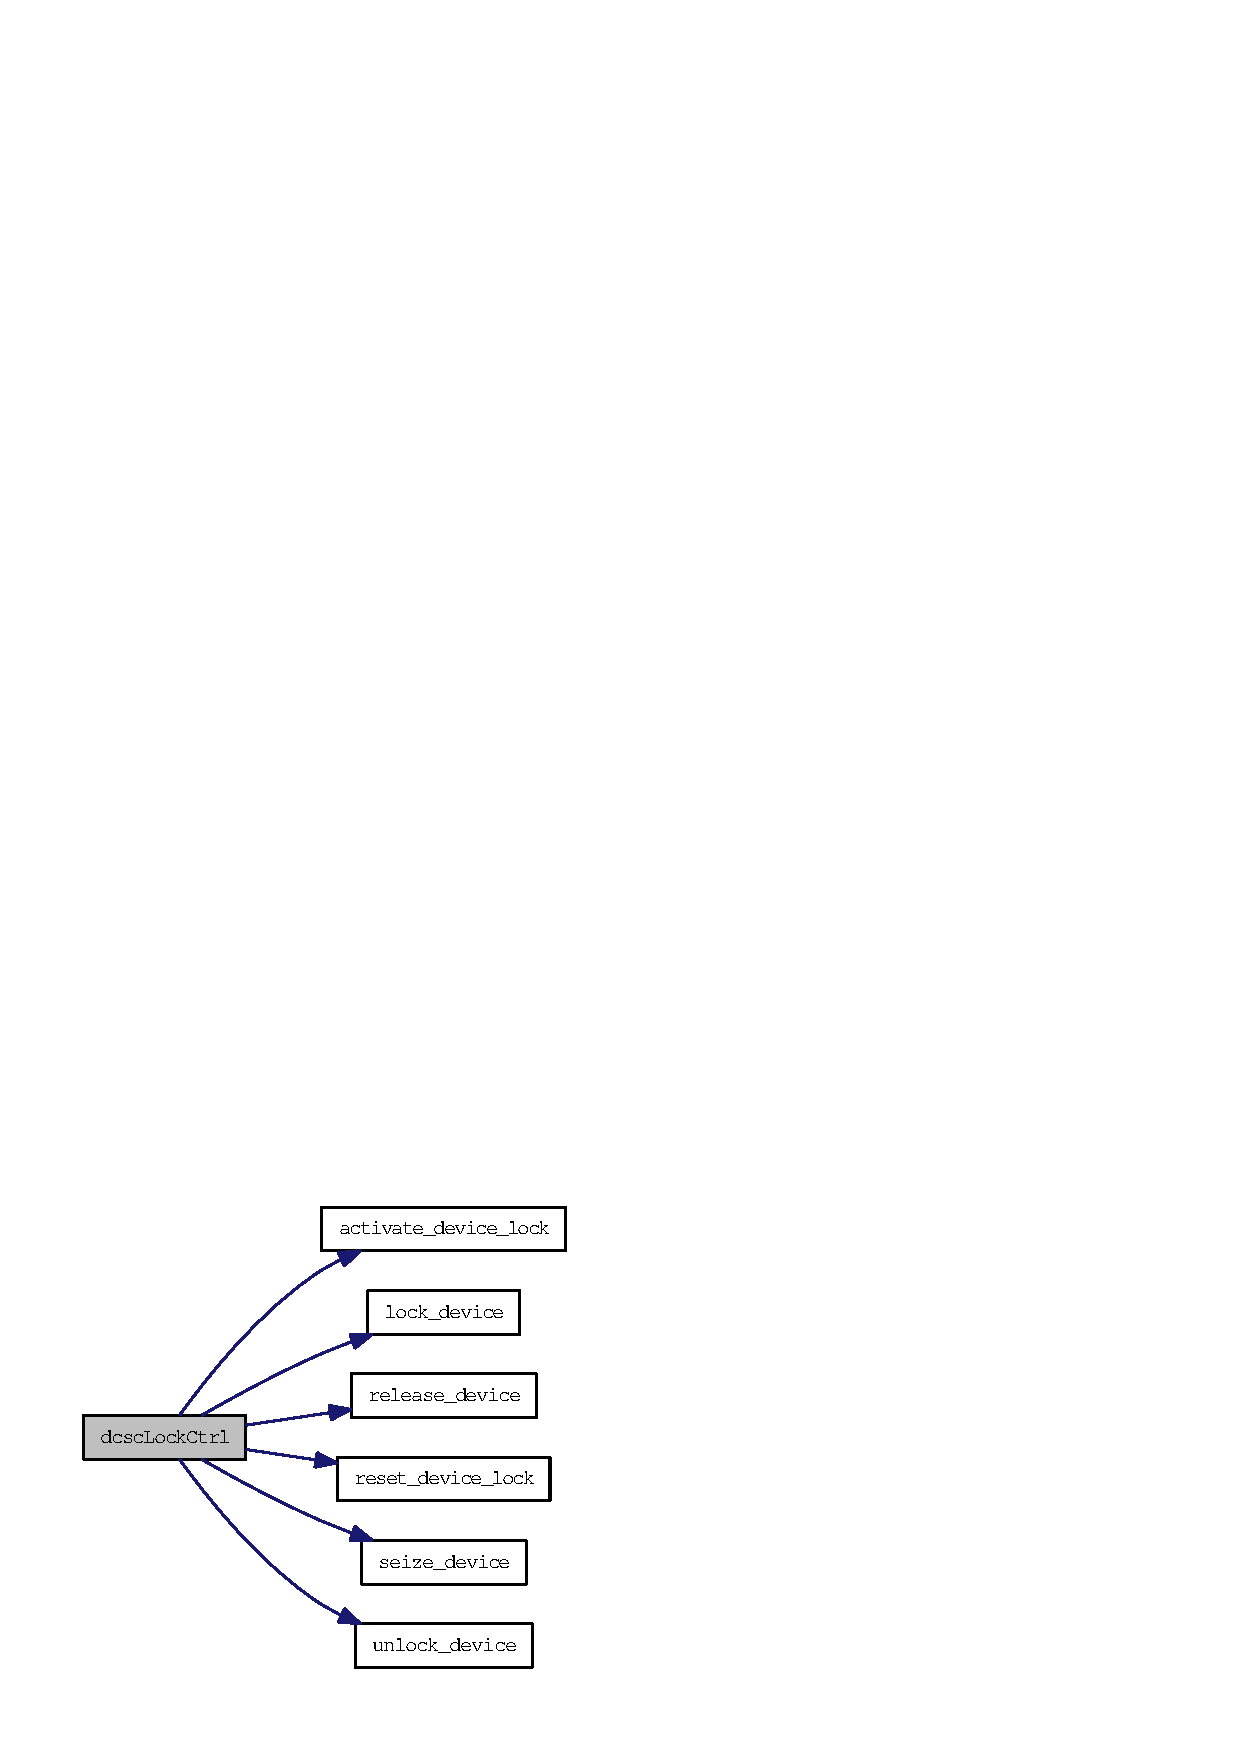
\includegraphics[width=138pt]{group__dcsc__msg__buffer__access_gb01774a452cb68f631a87d2d77ac79a5_cgraph}
\end{center}
\end{figure}
\hypertarget{group__dcsc__msg__buffer__access_g4f25fcb80c8fad99d5d72f96e72bd941}{
\index{dcsc_msg_buffer_access@{dcsc\_\-msg\_\-buffer\_\-access}!dcscPrepareMessageBuffer@{dcscPrepareMessageBuffer}}
\index{dcscPrepareMessageBuffer@{dcscPrepareMessageBuffer}!dcsc_msg_buffer_access@{dcsc\_\-msg\_\-buffer\_\-access}}
\subsubsection[dcscPrepareMessageBuffer]{\setlength{\rightskip}{0pt plus 5cm}int dcsc\-Prepare\-Message\-Buffer (\_\-\_\-u32 $\ast$$\ast$ {\em pp\-Buffer}, int $\ast$ {\em p\-Size}, unsigned int {\em cmd\-ID}, unsigned int {\em flags})}}
\label{group__dcsc__msg__buffer__access_g4f25fcb80c8fad99d5d72f96e72bd941}


Prepare the message buffer for a specific command. 

Creation and destruction of the buffer is handled by the interface internally {\bf DO NOT DELETE THIS BUFFER}.\par
 {\bf Note:} This function is forseen but not yet implemented \begin{Desc}
\item[Parameters:]
\begin{description}
\item[{\em pp\-Buffer}]target to receive the buffer pointer \item[{\em p\-Size}]target to receive the buffer size \item[{\em cmd\-ID}]command ID to prepare the buffer for \item[{\em flags}]for future extensions (e.g. preparation for compressed pedestal data) \end{description}
\end{Desc}
\begin{Desc}
\item[Returns:]pointer to buffer where the data words can directly be stored to, the information word and the markers and check sum are written by the interface. \end{Desc}


Definition at line 1600 of file dcsc\-Msg\-Buffer\-Interface.c.\hypertarget{group__dcsc__msg__buffer__access_gf7be7371f7530e8eb6e07e6f0d969b04}{
\index{dcsc_msg_buffer_access@{dcsc\_\-msg\_\-buffer\_\-access}!dcscProvideMessageBuffer@{dcscProvideMessageBuffer}}
\index{dcscProvideMessageBuffer@{dcscProvideMessageBuffer}!dcsc_msg_buffer_access@{dcsc\_\-msg\_\-buffer\_\-access}}
\subsubsection[dcscProvideMessageBuffer]{\setlength{\rightskip}{0pt plus 5cm}int dcsc\-Provide\-Message\-Buffer (\_\-\_\-u32 $\ast$$\ast$ {\em pp\-Buffer}, int $\ast$ {\em p\-Size})}}
\label{group__dcsc__msg__buffer__access_gf7be7371f7530e8eb6e07e6f0d969b04}


Provide the message buffer for direct access. 

Creation and destruction of the buffer is handled by the interface internally {\bf DO NOT DELETE THIS BUFFER}.\par
 {\bf Note:} This function is forseen but not yet implemented \begin{Desc}
\item[Parameters:]
\begin{description}
\item[{\em pp\-Buffer}]target to receive the buffer pointer \item[{\em p\-Size}]target to receive the buffer size \end{description}
\end{Desc}
\begin{Desc}
\item[Returns:]pointer to buffer, the caller is supposed to encode the complete message buffer, including the information word, the markers and data as well as check sum. The interface does not alter it. \end{Desc}


Definition at line 1575 of file dcsc\-Msg\-Buffer\-Interface.c.\hypertarget{group__dcsc__msg__buffer__access_gfc4448a8f5f9654cf54ad494f1558594}{
\index{dcsc_msg_buffer_access@{dcsc\_\-msg\_\-buffer\_\-access}!initRcuAccess@{initRcuAccess}}
\index{initRcuAccess@{initRcuAccess}!dcsc_msg_buffer_access@{dcsc\_\-msg\_\-buffer\_\-access}}
\subsubsection[initRcuAccess]{\setlength{\rightskip}{0pt plus 5cm}int init\-Rcu\-Access (const char $\ast$ {\em p\-Device\-Name})}}
\label{group__dcsc__msg__buffer__access_gfc4448a8f5f9654cf54ad494f1558594}


Initialize the interface. 

The device will be opened and some other other internal states initialized. \begin{Desc}
\item[Parameters:]
\begin{description}
\item[{\em p\-Device\-Name,:}]name of the device node, if NULL: /dev/dcsc as default \end{description}
\end{Desc}
\begin{Desc}
\item[Returns:]neg. error code if failed\par
 -ENOSPC : can not get the size of the interface buffers, or buffers too small\par
 -ENOENT : can not open device \end{Desc}


Definition at line 558 of file dcsc\-Msg\-Buffer\-Interface.c.

References init\-Rcu\-Access\-Ext().

Referenced by main().

Here is the call graph for this function:\begin{figure}[H]
\begin{center}
\leavevmode
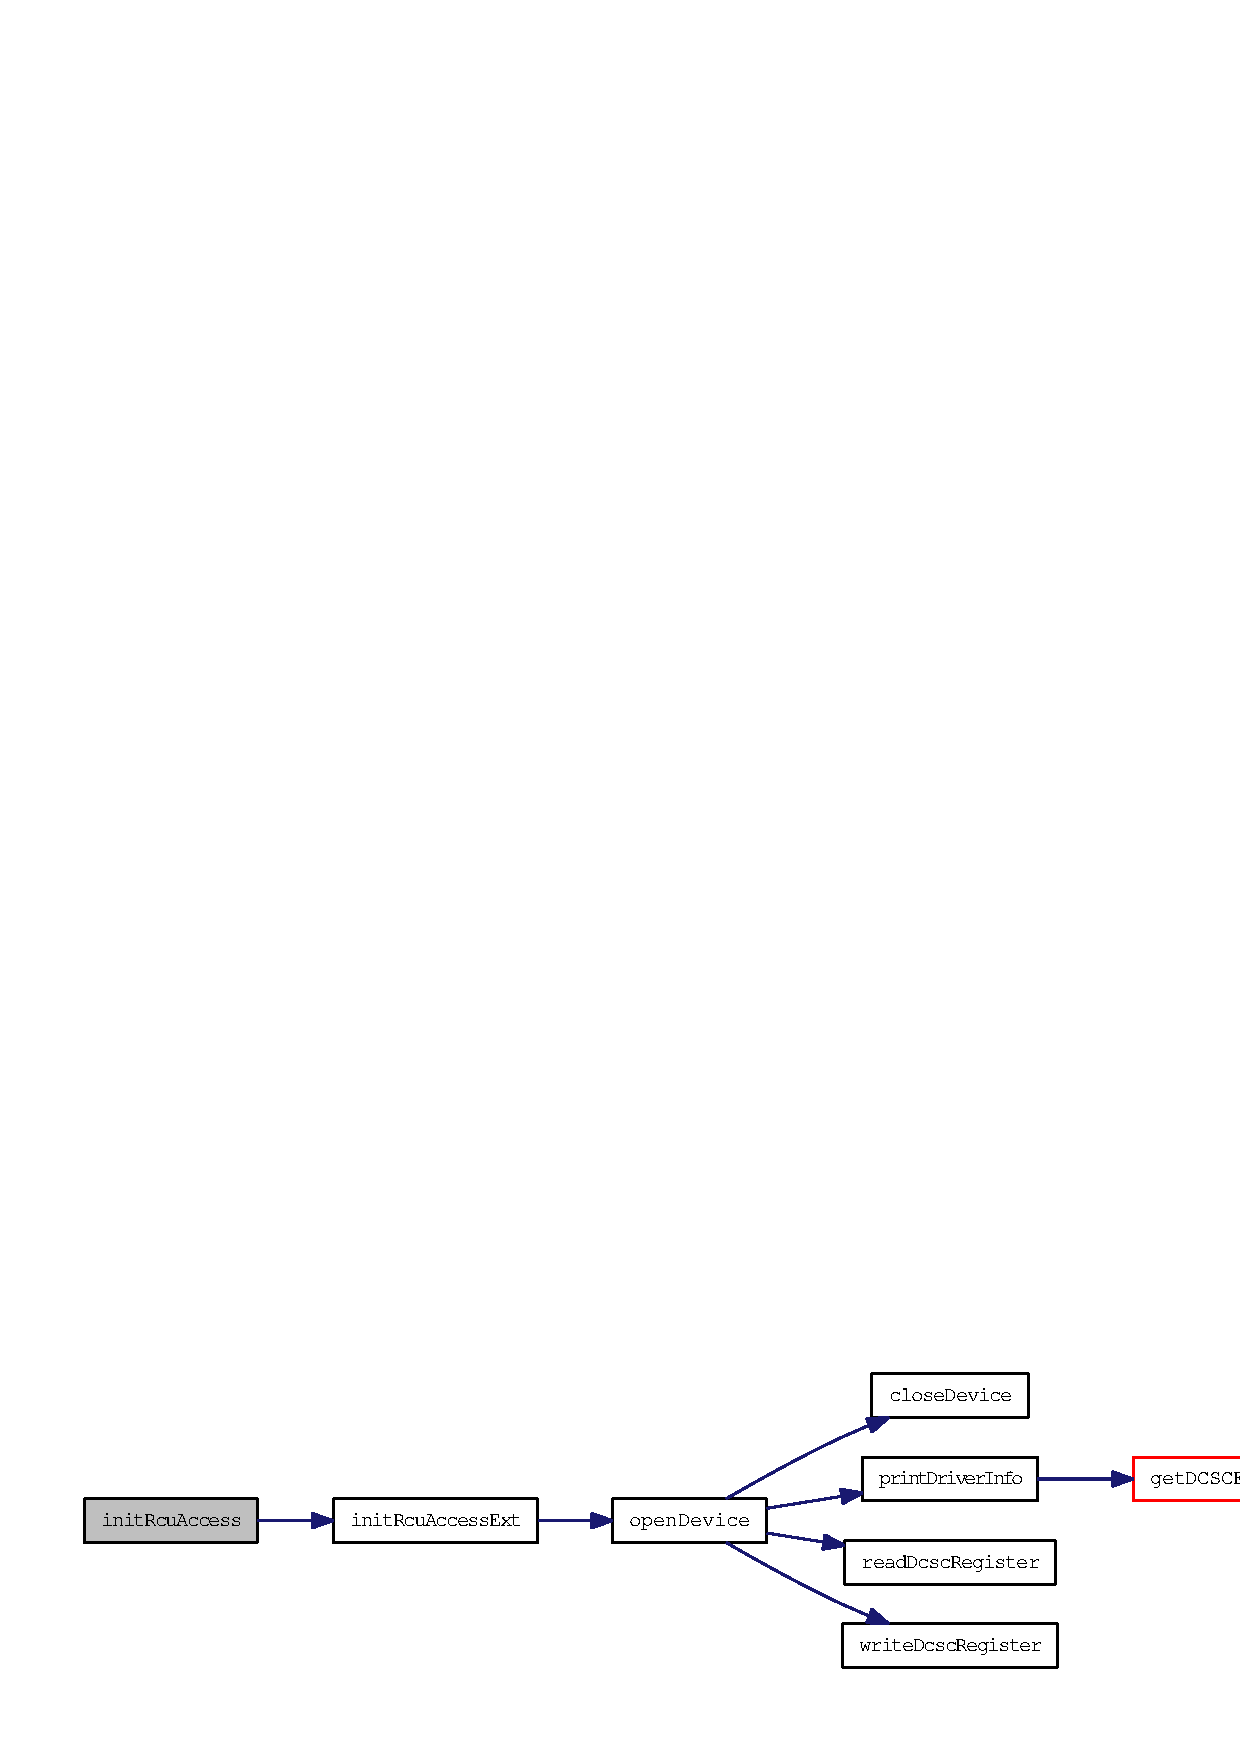
\includegraphics[width=350pt]{group__dcsc__msg__buffer__access_gfc4448a8f5f9654cf54ad494f1558594_cgraph}
\end{center}
\end{figure}
\hypertarget{group__dcsc__msg__buffer__access_g95f13464dd4da9231a53e7adbb0e7d4e}{
\index{dcsc_msg_buffer_access@{dcsc\_\-msg\_\-buffer\_\-access}!initRcuAccessExt@{initRcuAccessExt}}
\index{initRcuAccessExt@{initRcuAccessExt}!dcsc_msg_buffer_access@{dcsc\_\-msg\_\-buffer\_\-access}}
\subsubsection[initRcuAccessExt]{\setlength{\rightskip}{0pt plus 5cm}int init\-Rcu\-Access\-Ext (const char $\ast$ {\em p\-Device\-Name}, \hyperlink{structdcscInitArguments__t}{Tdcsc\-Init\-Arguments} $\ast$ {\em p\-Arg})}}
\label{group__dcsc__msg__buffer__access_g95f13464dd4da9231a53e7adbb0e7d4e}


Extended initialization. 

The function allows beside the device name a couple of other parameters to adjust the interface behavior. \begin{Desc}
\item[Parameters:]
\begin{description}
\item[{\em p\-Device\-Name}]name of the device node, if NULL: /dev/dcsc as default \item[{\em flags}]logical or of the following flags \item[{\em i\-MIBSize}]size of the MIB, used for encoding of message blocks \end{description}
\end{Desc}
\begin{Desc}
\item[Returns:]neg. error code if failed\par
 -ENOSPC : can not get the size of the interface buffers, or buffers too small\par
 -ENOENT : can not open device \end{Desc}


Definition at line 565 of file dcsc\-Msg\-Buffer\-Interface.c.

References DCSC\_\-INIT\_\-APPEND, DCSC\_\-INIT\_\-ENCODE, DCSC\_\-SKIP\_\-DRV\_\-ADPT, dcsc\-Init\-Arguments\_\-t::flags, g\_\-dcsc\-Flags, g\_\-verbosity, dcsc\-Init\-Arguments\_\-t::i\-MIBSize, dcsc\-Init\-Arguments\_\-t::i\-Verbosity, message\_\-in\_\-buffer\_\-size, and open\-Device().

Referenced by init\-Rcu\-Access(), and main().

Here is the call graph for this function:\begin{figure}[H]
\begin{center}
\leavevmode
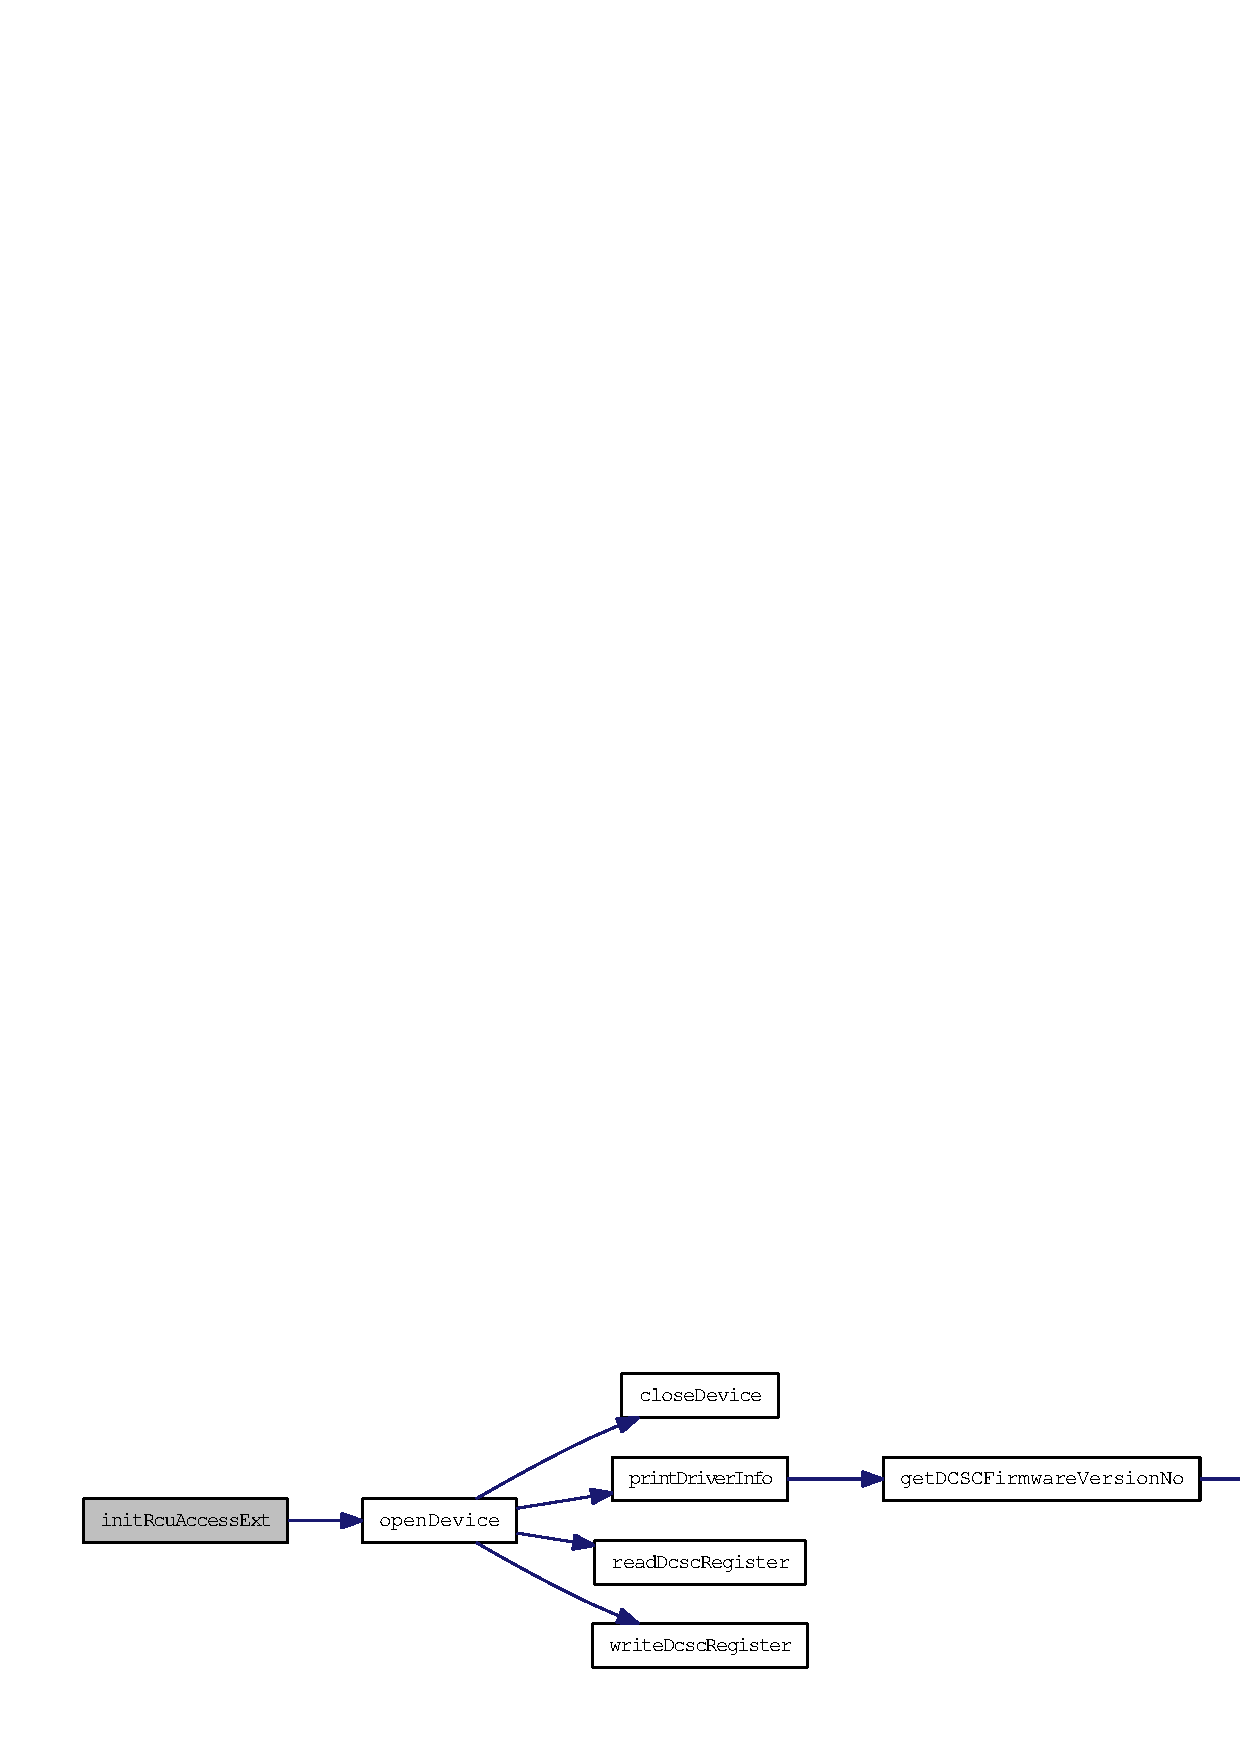
\includegraphics[width=351pt]{group__dcsc__msg__buffer__access_g95f13464dd4da9231a53e7adbb0e7d4e_cgraph}
\end{center}
\end{figure}
\hypertarget{group__dcsc__msg__buffer__access_g7a5b0d57fbd0a68206468a01b0a63520}{
\index{dcsc_msg_buffer_access@{dcsc\_\-msg\_\-buffer\_\-access}!msgBufReadRegister@{msgBufReadRegister}}
\index{msgBufReadRegister@{msgBufReadRegister}!dcsc_msg_buffer_access@{dcsc\_\-msg\_\-buffer\_\-access}}
\subsubsection[msgBufReadRegister]{\setlength{\rightskip}{0pt plus 5cm}int msg\-Buf\-Read\-Register (int {\em reg})}}
\label{group__dcsc__msg__buffer__access_g7a5b0d57fbd0a68206468a01b0a63520}


Read the value of a register from the register buffer. 

Originally, registers were 8 bit wide, but in the implementation of the message buffer interface in the DCS board firmware the addressing was 32 bit wide. Thats why register numbers correspond to register addresses = 4$\ast$reg\-No. \begin{Desc}
\item[Parameters:]
\begin{description}
\item[{\em reg}]\# of register \end{description}
\end{Desc}
\begin{Desc}
\item[Returns:]8 bit value of the register \end{Desc}


Definition at line 2078 of file dcsc\-Msg\-Buffer\-Interface.c.

References GENERAL\_\-CTRL\_\-REG\_\-ADDR, and read\-Dcsc\-Register().

Referenced by exec\-Reg\-Read\-Cmd().

Here is the call graph for this function:\begin{figure}[H]
\begin{center}
\leavevmode
\includegraphics[width=201pt]{group__dcsc__msg__buffer__access_g7a5b0d57fbd0a68206468a01b0a63520_cgraph}
\end{center}
\end{figure}
\hypertarget{group__dcsc__msg__buffer__access_g82e19c9d34c7ecebcba115d2a6393b6c}{
\index{dcsc_msg_buffer_access@{dcsc\_\-msg\_\-buffer\_\-access}!msgBufWriteRegister@{msgBufWriteRegister}}
\index{msgBufWriteRegister@{msgBufWriteRegister}!dcsc_msg_buffer_access@{dcsc\_\-msg\_\-buffer\_\-access}}
\subsubsection[msgBufWriteRegister]{\setlength{\rightskip}{0pt plus 5cm}int msg\-Buf\-Write\-Register (int {\em reg}, unsigned char {\em value})}}
\label{group__dcsc__msg__buffer__access_g82e19c9d34c7ecebcba115d2a6393b6c}


Write an 8 bit value to a register of the register buffer. 

The same as in \hyperlink{group__dcsc__msg__buffer__access_g7a5b0d57fbd0a68206468a01b0a63520}{msg\-Buf\-Read\-Register} applies for the register addressing. \begin{Desc}
\item[Parameters:]
\begin{description}
\item[{\em reg}]\# of register \item[{\em value}]8 bit value to write \end{description}
\end{Desc}
\begin{Desc}
\item[Returns:]8 bit value of the register after write \end{Desc}


Definition at line 2086 of file dcsc\-Msg\-Buffer\-Interface.c.

References GENERAL\_\-CTRL\_\-REG\_\-ADDR, and write\-Dcsc\-Register().

Referenced by exec\-Reg\-Write\-Cmd().

Here is the call graph for this function:\begin{figure}[H]
\begin{center}
\leavevmode
\includegraphics[width=203pt]{group__dcsc__msg__buffer__access_g82e19c9d34c7ecebcba115d2a6393b6c_cgraph}
\end{center}
\end{figure}
\hypertarget{group__dcsc__msg__buffer__access_g1b3027d209be85e9a8fbd14864c4b442}{
\index{dcsc_msg_buffer_access@{dcsc\_\-msg\_\-buffer\_\-access}!printBufferHex@{printBufferHex}}
\index{printBufferHex@{printBufferHex}!dcsc_msg_buffer_access@{dcsc\_\-msg\_\-buffer\_\-access}}
\subsubsection[printBufferHex]{\setlength{\rightskip}{0pt plus 5cm}void print\-Buffer\-Hex (unsigned char $\ast$ {\em p\-Buffer}, int {\em i\-Buffer\-Size}, int {\em word\-Size}, const char $\ast$ {\em p\-Message})}}
\label{group__dcsc__msg__buffer__access_g1b3027d209be85e9a8fbd14864c4b442}


Print content of a buffer hexadecimal. 

The content is assumed to be little endian (LSB first). \begin{Desc}
\item[Parameters:]
\begin{description}
\item[{\em p\-Buffer}]pointer to buffer \item[{\em i\-Buffer\-Size}]size of the buffer in byte \item[{\em i\-Word\-Size}]number of bytes in one word (1,2 or 4) \item[{\em p\-Message}]an optional message \end{description}
\end{Desc}


Definition at line 345 of file dcsc\-Msg\-Buffer\-Interface.c.

Referenced by check\-Msgin\-Buffer(), exec\-Write\-Cmd(), get\-Cmd\-Result(), print\-Buffer\-Hex\-Formatted(), rcu\-Flash\-ID(), rcu\-Multiple\-Read\-Ext(), rcu\-Single\-Read\-Ext(), and send\-Rcu\-Command().\hypertarget{group__dcsc__msg__buffer__access_gc44ca908f157f8de95b81638e298e08e}{
\index{dcsc_msg_buffer_access@{dcsc\_\-msg\_\-buffer\_\-access}!printBufferHexFormatted@{printBufferHexFormatted}}
\index{printBufferHexFormatted@{printBufferHexFormatted}!dcsc_msg_buffer_access@{dcsc\_\-msg\_\-buffer\_\-access}}
\subsubsection[printBufferHexFormatted]{\setlength{\rightskip}{0pt plus 5cm}void print\-Buffer\-Hex\-Formatted (unsigned char $\ast$ {\em p\-Buffer}, int {\em i\-Buffer\-Size}, int {\em i\-Word\-Size}, int {\em i\-Words\-Per\-Row}, int {\em i\-Start\-Address}, const char $\ast$ {\em p\-Message})}}
\label{group__dcsc__msg__buffer__access_gc44ca908f157f8de95b81638e298e08e}


Print content of a buffer hexadecimal formated with the address. 

The function formats the buffer to hexadecimal ascii with a dedicated number of words per row. Each row is preceeded by the address. The content is assumed to be little endian (LSB first) \begin{Desc}
\item[Parameters:]
\begin{description}
\item[{\em p\-Buffer}]pointer to buffer \item[{\em i\-Buffer\-Size}]size of the buffer in byte \item[{\em i\-Word\-Size}]number of bytes in one word (1,2 or 4) \item[{\em i\-Words\-Per\-Row}]number of words in one row \item[{\em i\-Start\-Address}]start address for the output \item[{\em p\-Message}]an optional message \end{description}
\end{Desc}


Definition at line 369 of file dcsc\-Msg\-Buffer\-Interface.c.

References print\-Buffer\-Hex().

Here is the call graph for this function:\begin{figure}[H]
\begin{center}
\leavevmode
\includegraphics[width=150pt]{group__dcsc__msg__buffer__access_gc44ca908f157f8de95b81638e298e08e_cgraph}
\end{center}
\end{figure}
\hypertarget{group__dcsc__msg__buffer__access_g919bc832f5a0e82c07cfafd699b1b2ea}{
\index{dcsc_msg_buffer_access@{dcsc\_\-msg\_\-buffer\_\-access}!printDriverInfo@{printDriverInfo}}
\index{printDriverInfo@{printDriverInfo}!dcsc_msg_buffer_access@{dcsc\_\-msg\_\-buffer\_\-access}}
\subsubsection[printDriverInfo]{\setlength{\rightskip}{0pt plus 5cm}void print\-Driver\-Info (int {\em i\-Verbosity})}}
\label{group__dcsc__msg__buffer__access_g919bc832f5a0e82c07cfafd699b1b2ea}


Get driver info from the driver and print it. 

\begin{Desc}
\item[Parameters:]
\begin{description}
\item[{\em i\-Verbosity}]1 full text, 0 just a few messages \end{description}
\end{Desc}


Definition at line 1839 of file dcsc\-Msg\-Buffer\-Interface.c.

References DCSC\_\-REQUIRED\_\-DRIVER\_\-VERSION\_\-MAJOR, DCSC\_\-REQUIRED\_\-DRIVER\_\-VERSION\_\-MINOR, g\_\-file, get\-DCSCFirmware\-Version\-No(), IOCTL\_\-GET\_\-VERS\_\-STR\_\-SIZE, IOCTL\_\-GET\_\-VERSION, IOCTL\_\-GET\_\-VERSION\_\-V02, message\_\-in\_\-buffer\_\-size, message\_\-out\_\-buffer\_\-size, message\_\-regfile\_\-size, RCUBUS\_\-DRIVER\_\-VERSION\_\-MAJOR\_\-BITSHIFT, RCUBUS\_\-DRIVER\_\-VERSION\_\-MAJOR\_\-SIZE, RCUBUS\_\-DRIVER\_\-VERSION\_\-MINOR\_\-BITSHIFT, and RCUBUS\_\-DRIVER\_\-VERSION\_\-MINOR\_\-SIZE.

Referenced by open\-Device().

Here is the call graph for this function:\begin{figure}[H]
\begin{center}
\leavevmode
\includegraphics[width=287pt]{group__dcsc__msg__buffer__access_g919bc832f5a0e82c07cfafd699b1b2ea_cgraph}
\end{center}
\end{figure}
\hypertarget{group__dcsc__msg__buffer__access_gf74b29f8ded2feb57974c95e4863eac8}{
\index{dcsc_msg_buffer_access@{dcsc\_\-msg\_\-buffer\_\-access}!rcuBusControlCmd@{rcuBusControlCmd}}
\index{rcuBusControlCmd@{rcuBusControlCmd}!dcsc_msg_buffer_access@{dcsc\_\-msg\_\-buffer\_\-access}}
\subsubsection[rcuBusControlCmd]{\setlength{\rightskip}{0pt plus 5cm}int rcu\-Bus\-Control\-Cmd (int {\em i\-Cmd})}}
\label{group__dcsc__msg__buffer__access_gf74b29f8ded2feb57974c95e4863eac8}


Switch bits in the control register (firmware comstat). 

\begin{Desc}
\item[Parameters:]
\begin{description}
\item[{\em i\-Cmd}]buffer control command, see enums above \end{description}
\end{Desc}
\begin{Desc}
\item[Returns:]the (new) value of the control register, neg. error code if failed\par
 -EBADFD if interface in wrong state to perform the command\par
 -EIO if internal error (bits can not be changed)\par
 -EINVAL unknown command id \end{Desc}


Definition at line 2073 of file dcsc\-Msg\-Buffer\-Interface.c.

References rcu\-Bus\-Control\-Cmd\-Ext().

Referenced by calculate\-Stop\-Address(), ctrl\-Reg\-Status(), enter\-Flash\-State(), get\-Bus\-State(), and restore\-Bus\-State().

Here is the call graph for this function:\begin{figure}[H]
\begin{center}
\leavevmode
\includegraphics[width=154pt]{group__dcsc__msg__buffer__access_gf74b29f8ded2feb57974c95e4863eac8_cgraph}
\end{center}
\end{figure}
\hypertarget{group__dcsc__msg__buffer__access_g78e6fc883a098cf548e9d0ba618ecb16}{
\index{dcsc_msg_buffer_access@{dcsc\_\-msg\_\-buffer\_\-access}!rcuFlashErase@{rcuFlashErase}}
\index{rcuFlashErase@{rcuFlashErase}!dcsc_msg_buffer_access@{dcsc\_\-msg\_\-buffer\_\-access}}
\subsubsection[rcuFlashErase]{\setlength{\rightskip}{0pt plus 5cm}int rcu\-Flash\-Erase (int {\em start\-Sec}, int {\em stop\-Sec})}}
\label{group__dcsc__msg__buffer__access_g78e6fc883a098cf548e9d0ba618ecb16}


Erase sectors of the flash. 

\begin{Desc}
\item[Parameters:]
\begin{description}
\item[{\em first\-Sec}]the first sector to erase; if -1 erase all \item[{\em last\-Sec}]the last sector to erase \end{description}
\end{Desc}
\begin{Desc}
\item[Returns:]0 success, neg. error code if failed \end{Desc}


Definition at line 2311 of file dcsc\-Msg\-Buffer\-Interface.c.

References check\-State(), e\-Disable\-Flash, e\-Enable\-Flash, e\-Flash, e\-Flash\-Access\-Dcsc, FLASH\_\-ERASE\_\-SEC, FLASH\_\-ERASEALL, FLASH\_\-MULTI\_\-ERASE, g\_\-i\-Flash\-Access\-Mode, g\_\-verbosity, lock\_\-device(), mib\-Size, mk\-End\-Marker(), mk\-Frst\-Wrd(), mk\-Lst\-Wrd(), MSGBUF\_\-MODE\_\-FLASH, p\-Mib, RCU\_\-FLASH\_\-ADDRH, RCU\_\-FLASH\_\-ADDRL, RCU\_\-FLASH\_\-CMD, RCU\_\-FLASH\_\-ERASE\_\-WAITCYCLE, RCU\_\-FLASH\_\-ERASEALL, RCU\_\-FLASH\_\-ERASESEC, RCU\_\-FLASH\_\-MAX\_\-WAITSTATES, RCU\_\-FLASH\_\-STATE\_\-IDLE, RCU\_\-FLASH\_\-STATE\_\-MASK, RCU\_\-FLASH\_\-STATUS, rcu\-Bus\-Control\-Cmd\-Ext(), rcu\-Single\-Read(), rcu\-Single\-Write(), send\-Rcu\-Command(), and unlock\_\-device().

Referenced by exec\-Flash\-Erase(), exec\-Flash\-Eraseall(), and main().

Here is the call graph for this function:\begin{figure}[H]
\begin{center}
\leavevmode
\includegraphics[width=204pt]{group__dcsc__msg__buffer__access_g78e6fc883a098cf548e9d0ba618ecb16_cgraph}
\end{center}
\end{figure}
\hypertarget{group__dcsc__msg__buffer__access_g24164f14711ead31a7e542711f0a08b3}{
\index{dcsc_msg_buffer_access@{dcsc\_\-msg\_\-buffer\_\-access}!rcuFlashRead@{rcuFlashRead}}
\index{rcuFlashRead@{rcuFlashRead}!dcsc_msg_buffer_access@{dcsc\_\-msg\_\-buffer\_\-access}}
\subsubsection[rcuFlashRead]{\setlength{\rightskip}{0pt plus 5cm}int rcu\-Flash\-Read (\_\-\_\-u32 {\em address}, int {\em i\-Size}, \_\-\_\-u32 $\ast$ {\em p\-Data})}}
\label{group__dcsc__msg__buffer__access_g24164f14711ead31a7e542711f0a08b3}


Read a number of 16bit words from the flash memory. 

currently all communication is done through the message buffer \begin{Desc}
\item[Parameters:]
\begin{description}
\item[{\em address}]start location \item[{\em i\-Size}]number of words to read \item[{\em p\-Data}]buffer to receive the data, the function expect it to be of suitable size (i.e. i\-Size x wordsize) \end{description}
\end{Desc}
\begin{Desc}
\item[Returns:]number of read 32bit words, neg. error code if failed \end{Desc}


Definition at line 2223 of file dcsc\-Msg\-Buffer\-Interface.c.

References check\-State(), e\-Disable\-Flash, e\-Enable\-Flash, e\-Flash, e\-Flash\-Access\-Dcsc, g\_\-i\-Flash\-Access\-Mode, g\_\-verbosity, lock\_\-device(), MSGBUF\_\-MODE\_\-FLASH, RCU\_\-FLASH\_\-ADDRH, RCU\_\-FLASH\_\-ADDRL, RCU\_\-FLASH\_\-AHBSHFT, RCU\_\-FLASH\_\-AHMASK, RCU\_\-FLASH\_\-ALMASK, RCU\_\-FLASH\_\-CMD, RCU\_\-FLASH\_\-DEFAULT\_\-WAITCYCLE, RCU\_\-FLASH\_\-MAX\_\-WAITSTATES, RCU\_\-FLASH\_\-READCMD, RCU\_\-FLASH\_\-READRES, RCU\_\-FLASH\_\-SIZE, RCU\_\-FLASH\_\-STATE\_\-IDLE, RCU\_\-FLASH\_\-STATE\_\-MASK, RCU\_\-FLASH\_\-STATUS, rcu\-Bus\-Control\-Cmd\-Ext(), rcu\-Multiple\-Read\-Ext(), rcu\-Single\-Read(), rcu\-Single\-Write(), and unlock\_\-device().

Referenced by exec\-Read\-Cmd(), and exec\-Write\-Cmd().

Here is the call graph for this function:\begin{figure}[H]
\begin{center}
\leavevmode
\includegraphics[width=203pt]{group__dcsc__msg__buffer__access_g24164f14711ead31a7e542711f0a08b3_cgraph}
\end{center}
\end{figure}
\hypertarget{group__dcsc__msg__buffer__access_g88debbd24075d2031add9459e4d90e2b}{
\index{dcsc_msg_buffer_access@{dcsc\_\-msg\_\-buffer\_\-access}!rcuFlashWrite@{rcuFlashWrite}}
\index{rcuFlashWrite@{rcuFlashWrite}!dcsc_msg_buffer_access@{dcsc\_\-msg\_\-buffer\_\-access}}
\subsubsection[rcuFlashWrite]{\setlength{\rightskip}{0pt plus 5cm}int rcu\-Flash\-Write (\_\-\_\-u32 {\em address}, \_\-\_\-u32 $\ast$ {\em p\-Data}, int {\em i\-Size}, int {\em i\-Data\-Size})}}
\label{group__dcsc__msg__buffer__access_g88debbd24075d2031add9459e4d90e2b}


Write to the RCU flash. 

currently all communication is done through the message buffer \begin{Desc}
\item[Parameters:]
\begin{description}
\item[{\em address}]start location \item[{\em p\-Data}]buffer containing the data \item[{\em i\-Size}]number of words to write \item[{\em i\-Data\-Size}]size of one word in bytes, allowed 1,2 \end{description}
\end{Desc}
\begin{Desc}
\item[Returns:]\end{Desc}


Definition at line 2130 of file dcsc\-Msg\-Buffer\-Interface.c.

References check\-State(), e\-Disable\-Flash, e\-Enable\-Flash, e\-Flash, e\-Flash\-Access\-Dcsc, g\_\-i\-Flash\-Access\-Mode, g\_\-verbosity, lock\_\-device(), MSGBUF\_\-MODE\_\-FLASH, RCU\_\-FLASH\_\-ADDRH, RCU\_\-FLASH\_\-ADDRL, RCU\_\-FLASH\_\-AHBSHFT, RCU\_\-FLASH\_\-AHMASK, RCU\_\-FLASH\_\-ALMASK, RCU\_\-FLASH\_\-CMD, RCU\_\-FLASH\_\-DATA, RCU\_\-FLASH\_\-DEFAULT\_\-WAITCYCLE, RCU\_\-FLASH\_\-MAX\_\-WAITSTATES, RCU\_\-FLASH\_\-SIZE, RCU\_\-FLASH\_\-STATE\_\-IDLE, RCU\_\-FLASH\_\-STATE\_\-MASK, RCU\_\-FLASH\_\-STATUS, RCU\_\-FLASH\_\-WRITECMD, rcu\-Bus\-Control\-Cmd\-Ext(), rcu\-Multiple\-Write\-Ext(), rcu\-Single\-Read(), rcu\-Single\-Write(), and unlock\_\-device().

Referenced by do\-Flash\-Frame(), do\-Init(), do\-Scrubbing(), and exec\-Write\-Cmd().

Here is the call graph for this function:\begin{figure}[H]
\begin{center}
\leavevmode
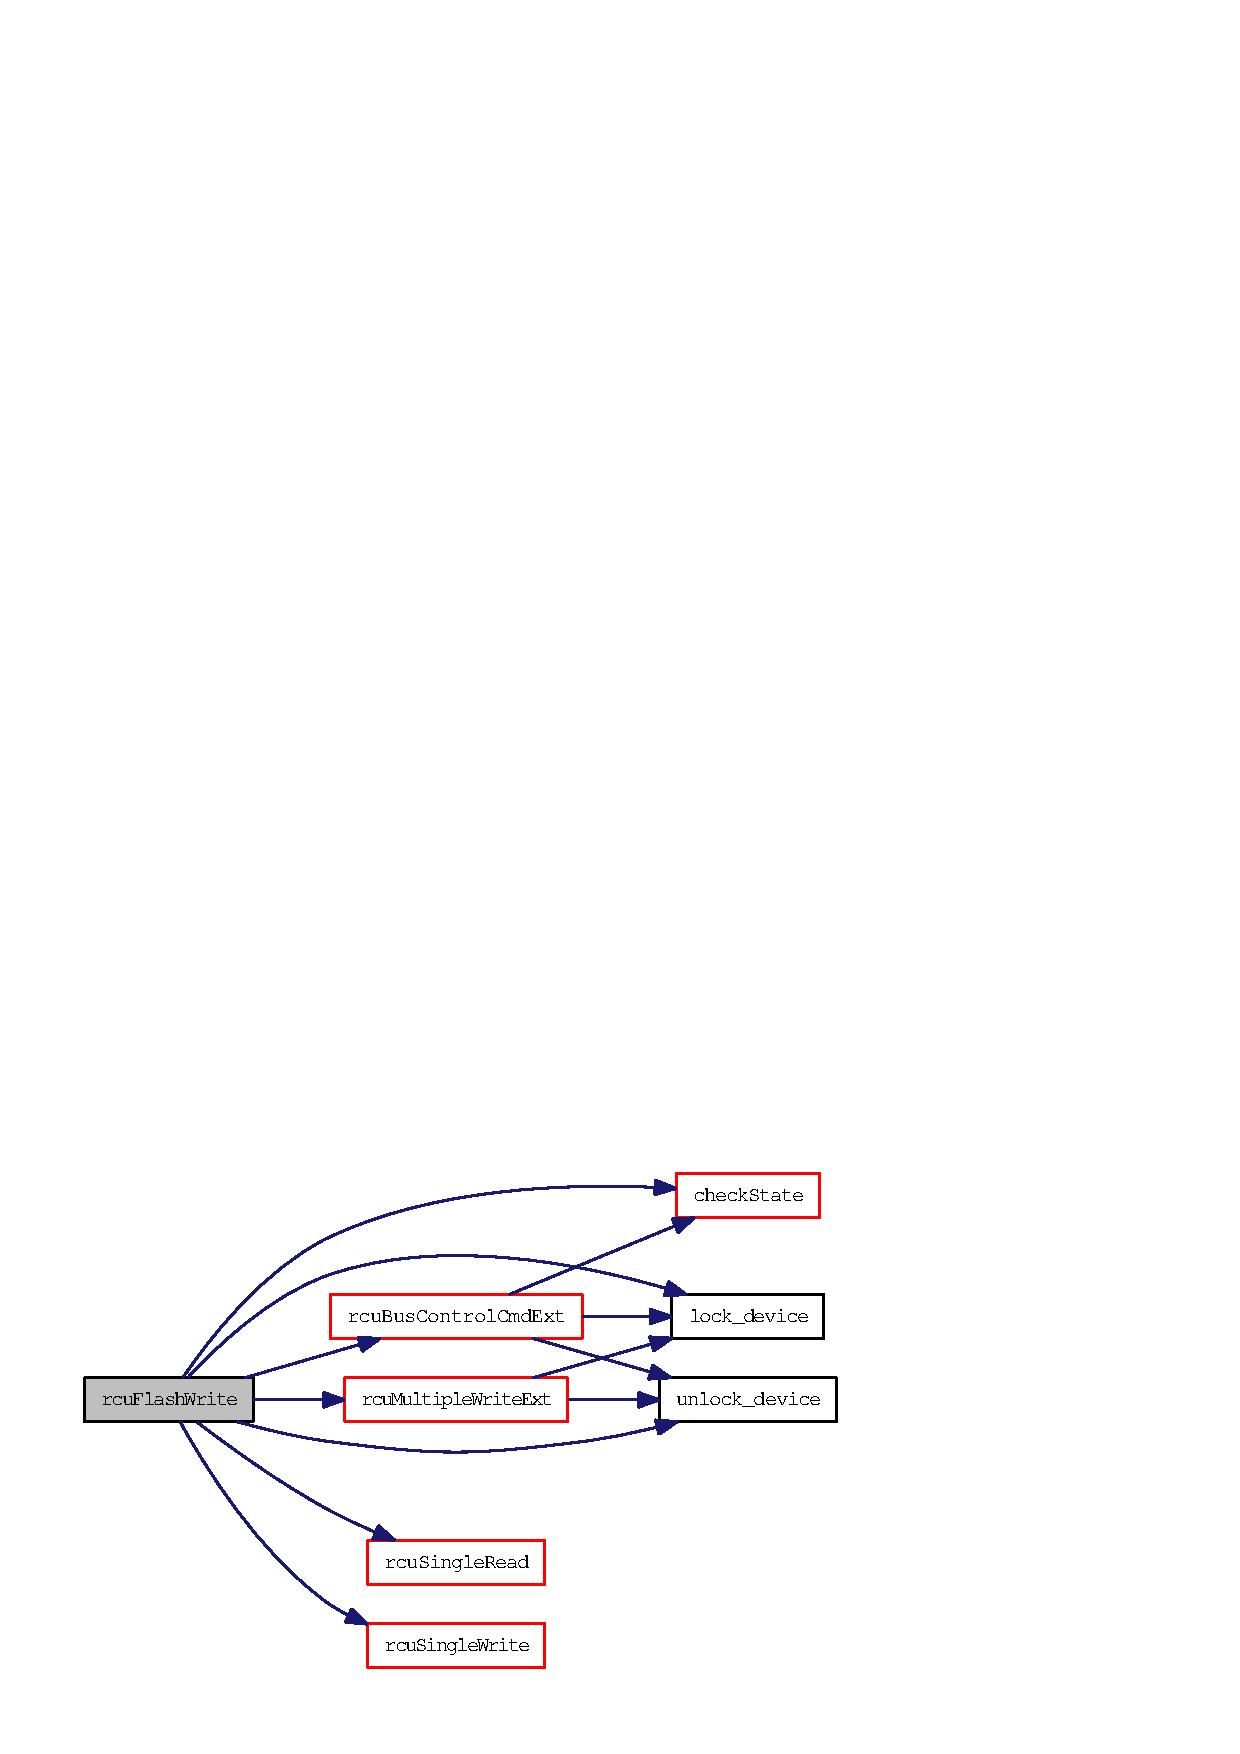
\includegraphics[width=203pt]{group__dcsc__msg__buffer__access_g88debbd24075d2031add9459e4d90e2b_cgraph}
\end{center}
\end{figure}
\hypertarget{group__dcsc__msg__buffer__access_g602216accce6913989f8b04b36157cd6}{
\index{dcsc_msg_buffer_access@{dcsc\_\-msg\_\-buffer\_\-access}!rcuMultipleRead@{rcuMultipleRead}}
\index{rcuMultipleRead@{rcuMultipleRead}!dcsc_msg_buffer_access@{dcsc\_\-msg\_\-buffer\_\-access}}
\subsubsection[rcuMultipleRead]{\setlength{\rightskip}{0pt plus 5cm}int rcu\-Multiple\-Read (\_\-\_\-u32 {\em address}, int {\em i\-Size}, \_\-\_\-u32 $\ast$ {\em p\-Data})}}
\label{group__dcsc__msg__buffer__access_g602216accce6913989f8b04b36157cd6}


Read a number of 32bit words beginning at a location. 

\begin{Desc}
\item[Parameters:]
\begin{description}
\item[{\em address}]16 bit address in RCU memory space \item[{\em i\-Size}]number of words to write \item[{\em p\-Data}]buffer to receive the data, the function expect it to be of suitable size (i.e. i\-Size x wordsize) \end{description}
\end{Desc}
\begin{Desc}
\item[Returns:]number of 32bit words which have been read, neg. error code if failed \end{Desc}


Definition at line 1566 of file dcsc\-Msg\-Buffer\-Interface.c.

References MSGBUF\_\-MODE\_\-MEMMAPPED, and rcu\-Multiple\-Read\-Ext().

Referenced by exec\-Read\-Cmd(), and main().

Here is the call graph for this function:\begin{figure}[H]
\begin{center}
\leavevmode
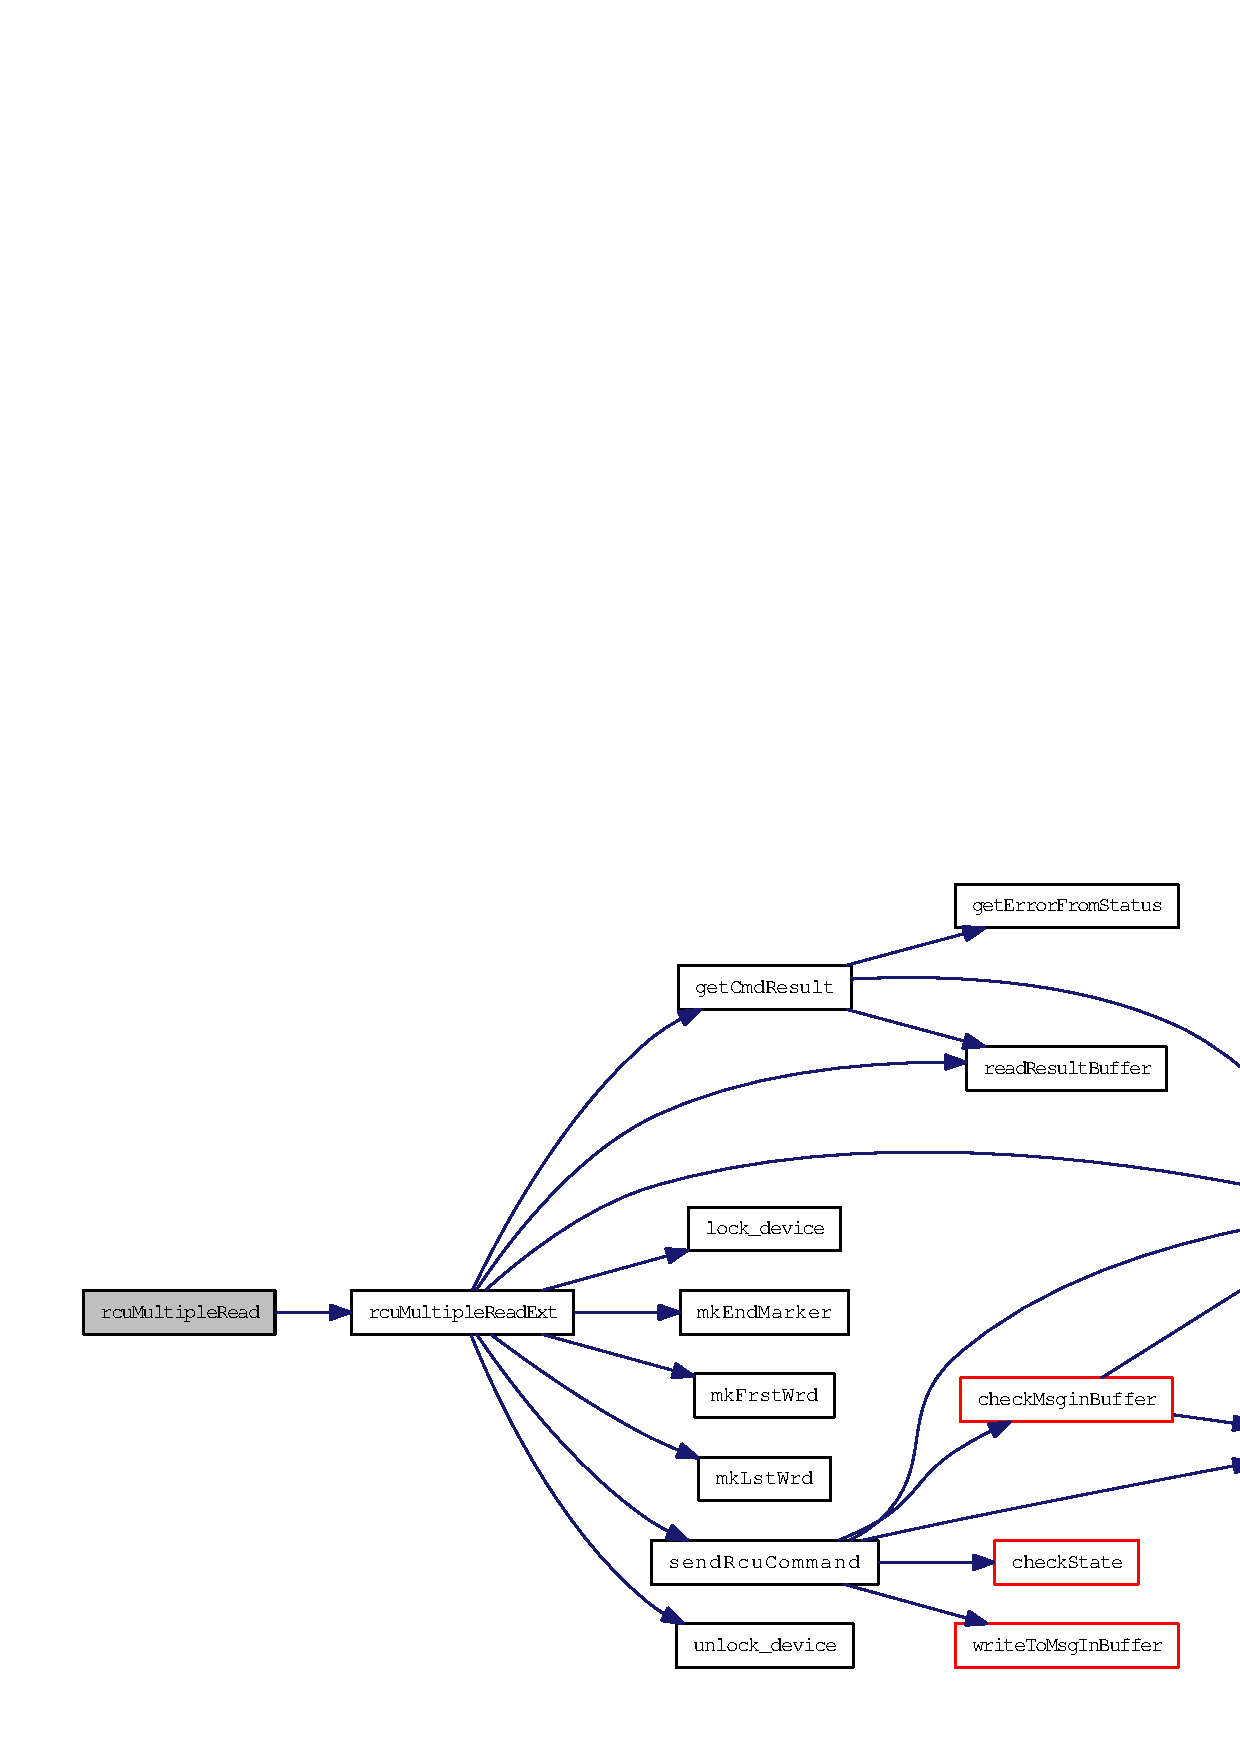
\includegraphics[width=356pt]{group__dcsc__msg__buffer__access_g602216accce6913989f8b04b36157cd6_cgraph}
\end{center}
\end{figure}
\hypertarget{group__dcsc__msg__buffer__access_ge20afbfc92c897546e37126188804309}{
\index{dcsc_msg_buffer_access@{dcsc\_\-msg\_\-buffer\_\-access}!rcuMultipleWrite@{rcuMultipleWrite}}
\index{rcuMultipleWrite@{rcuMultipleWrite}!dcsc_msg_buffer_access@{dcsc\_\-msg\_\-buffer\_\-access}}
\subsubsection[rcuMultipleWrite]{\setlength{\rightskip}{0pt plus 5cm}int rcu\-Multiple\-Write (\_\-\_\-u32 {\em address}, \_\-\_\-u32 $\ast$ {\em p\-Data}, int {\em i\-Size}, int {\em i\-Data\-Size})}}
\label{group__dcsc__msg__buffer__access_ge20afbfc92c897546e37126188804309}


Write a number of 32bit words beginning at a location. 

The function takes care for the size of the MIB and splits the operation if the amount of data to write exceeds the MIB size. The function expects data in little endian byte order \begin{Desc}
\item[Parameters:]
\begin{description}
\item[{\em address}]16 bit address in RCU memory space \item[{\em p\-Data}]buffer containing the data \item[{\em i\-Size}]number of words to write \item[{\em i\-Data\-Size}]size of one word in bytes, allowed 1 (8 bit), 2 (16 bit),3 (compressed 10 bit) or 4 (32 bit) -2 and -4 denote 16/32 bit words which get swapped \end{description}
\end{Desc}
\begin{Desc}
\item[Returns:]\end{Desc}


Definition at line 1549 of file dcsc\-Msg\-Buffer\-Interface.c.

References MSGBUF\_\-MODE\_\-MEMMAPPED, and rcu\-Multiple\-Write\-Ext().

Referenced by exec\-Write\-Cmd(), and init().

Here is the call graph for this function:\begin{figure}[H]
\begin{center}
\leavevmode
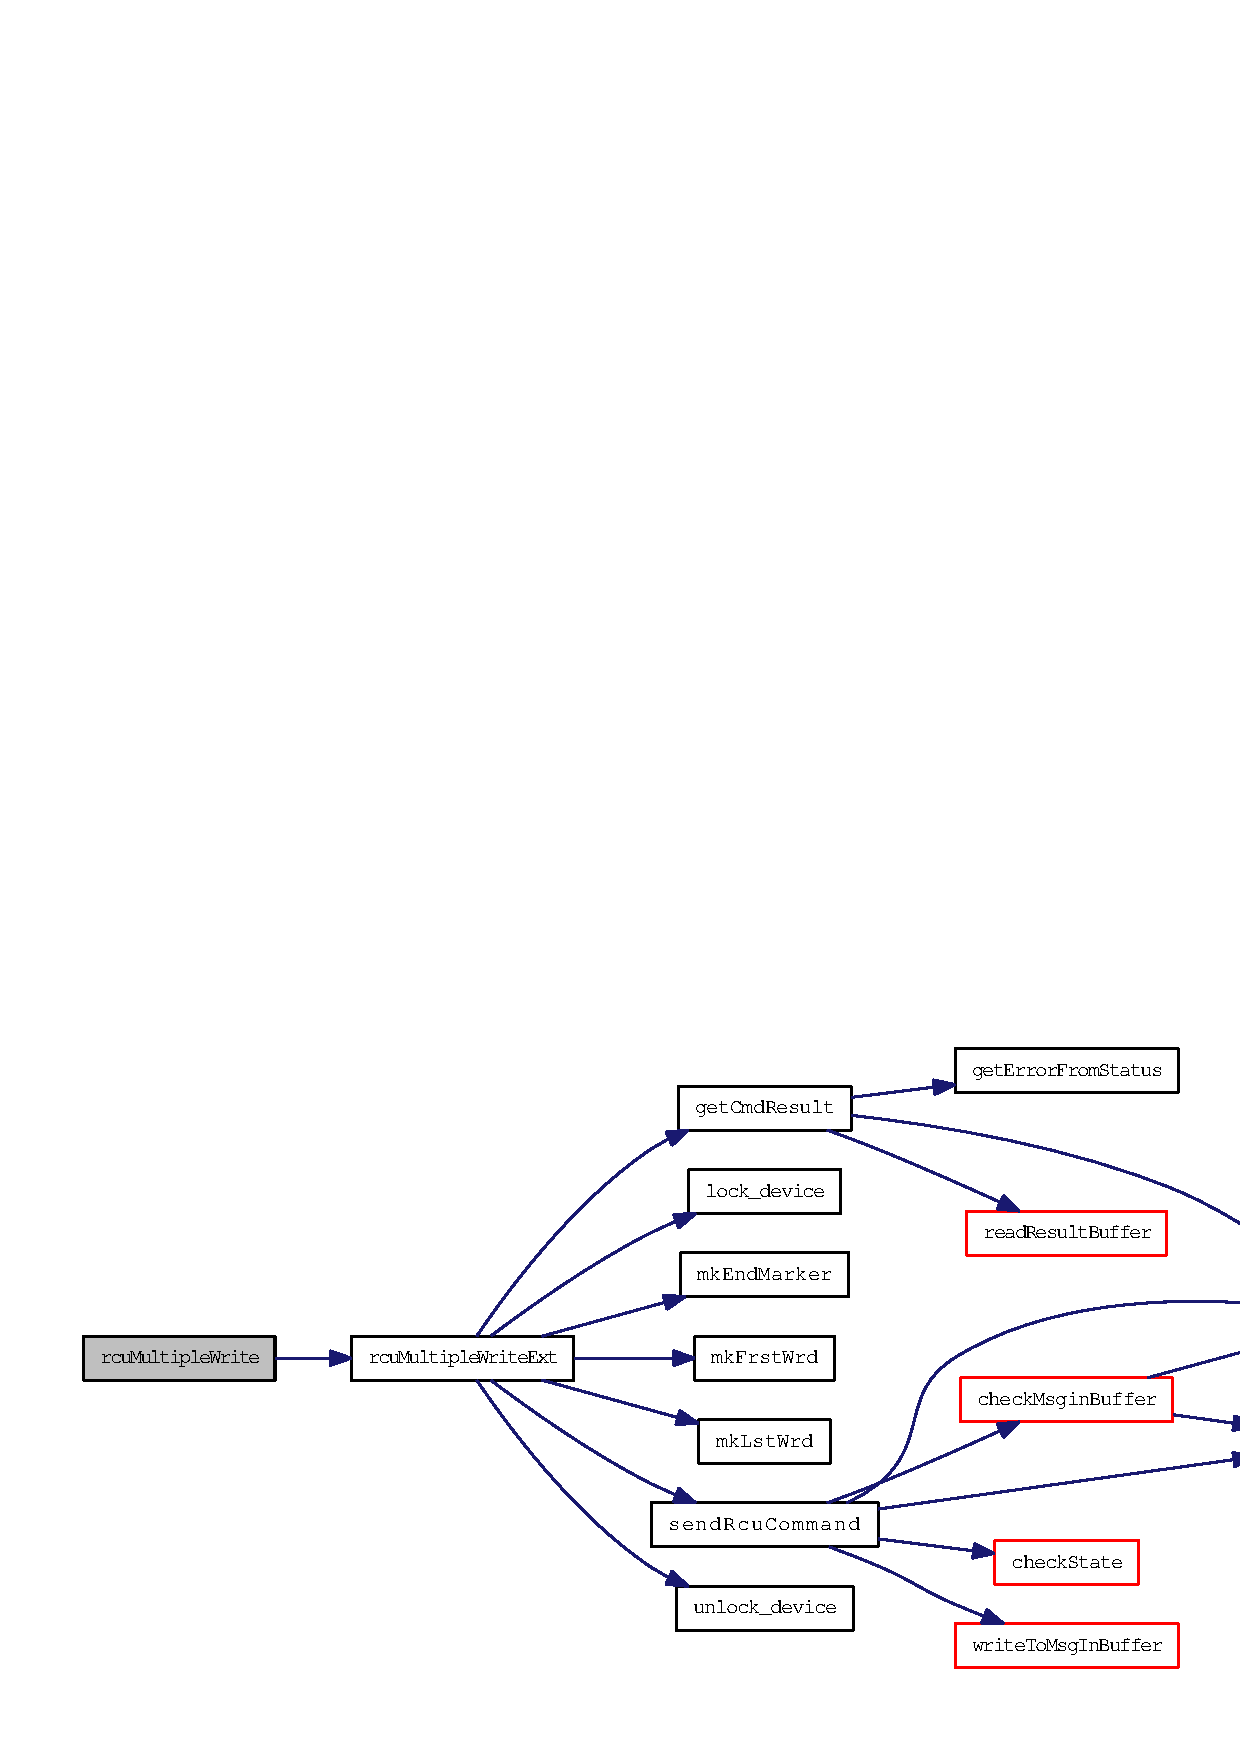
\includegraphics[width=356pt]{group__dcsc__msg__buffer__access_ge20afbfc92c897546e37126188804309_cgraph}
\end{center}
\end{figure}
\hypertarget{group__dcsc__msg__buffer__access_g339b5922513d0f0211d7962234faa24f}{
\index{dcsc_msg_buffer_access@{dcsc\_\-msg\_\-buffer\_\-access}!rcuSingleRead@{rcuSingleRead}}
\index{rcuSingleRead@{rcuSingleRead}!dcsc_msg_buffer_access@{dcsc\_\-msg\_\-buffer\_\-access}}
\subsubsection[rcuSingleRead]{\setlength{\rightskip}{0pt plus 5cm}int rcu\-Single\-Read (\_\-\_\-u32 {\em address}, \_\-\_\-u32 $\ast$ {\em p\-Data})}}
\label{group__dcsc__msg__buffer__access_g339b5922513d0f0211d7962234faa24f}


Read a single location (32bit word). 

\begin{Desc}
\item[Parameters:]
\begin{description}
\item[{\em address}]16 bit address in RCU memory space \item[{\em p\-Data}]buffer to receive the data \end{description}
\end{Desc}
\begin{Desc}
\item[Returns:]\end{Desc}


Definition at line 1557 of file dcsc\-Msg\-Buffer\-Interface.c.

References MSGBUF\_\-MODE\_\-MEMMAPPED, and rcu\-Single\-Read\-Ext().

Referenced by calculate\-Stop\-Address(), exec\-Read\-Cmd(), get\-DCSCFirmware\-Version\-No(), get\-Errorcounter\-Reg(), get\-Last\-Error\-Framenumber(), get\-Last\-Framenumber(), get\-Number\-Of\-Cycles(), rcu\-Flash\-Erase(), rcu\-Flash\-ID(), rcu\-Flash\-Read(), rcu\-Flash\-Reset(), rcu\-Flash\-Write(), read\-Err\-Reg(), read\-Status\-Reg(), and wait\-Condition().

Here is the call graph for this function:\begin{figure}[H]
\begin{center}
\leavevmode
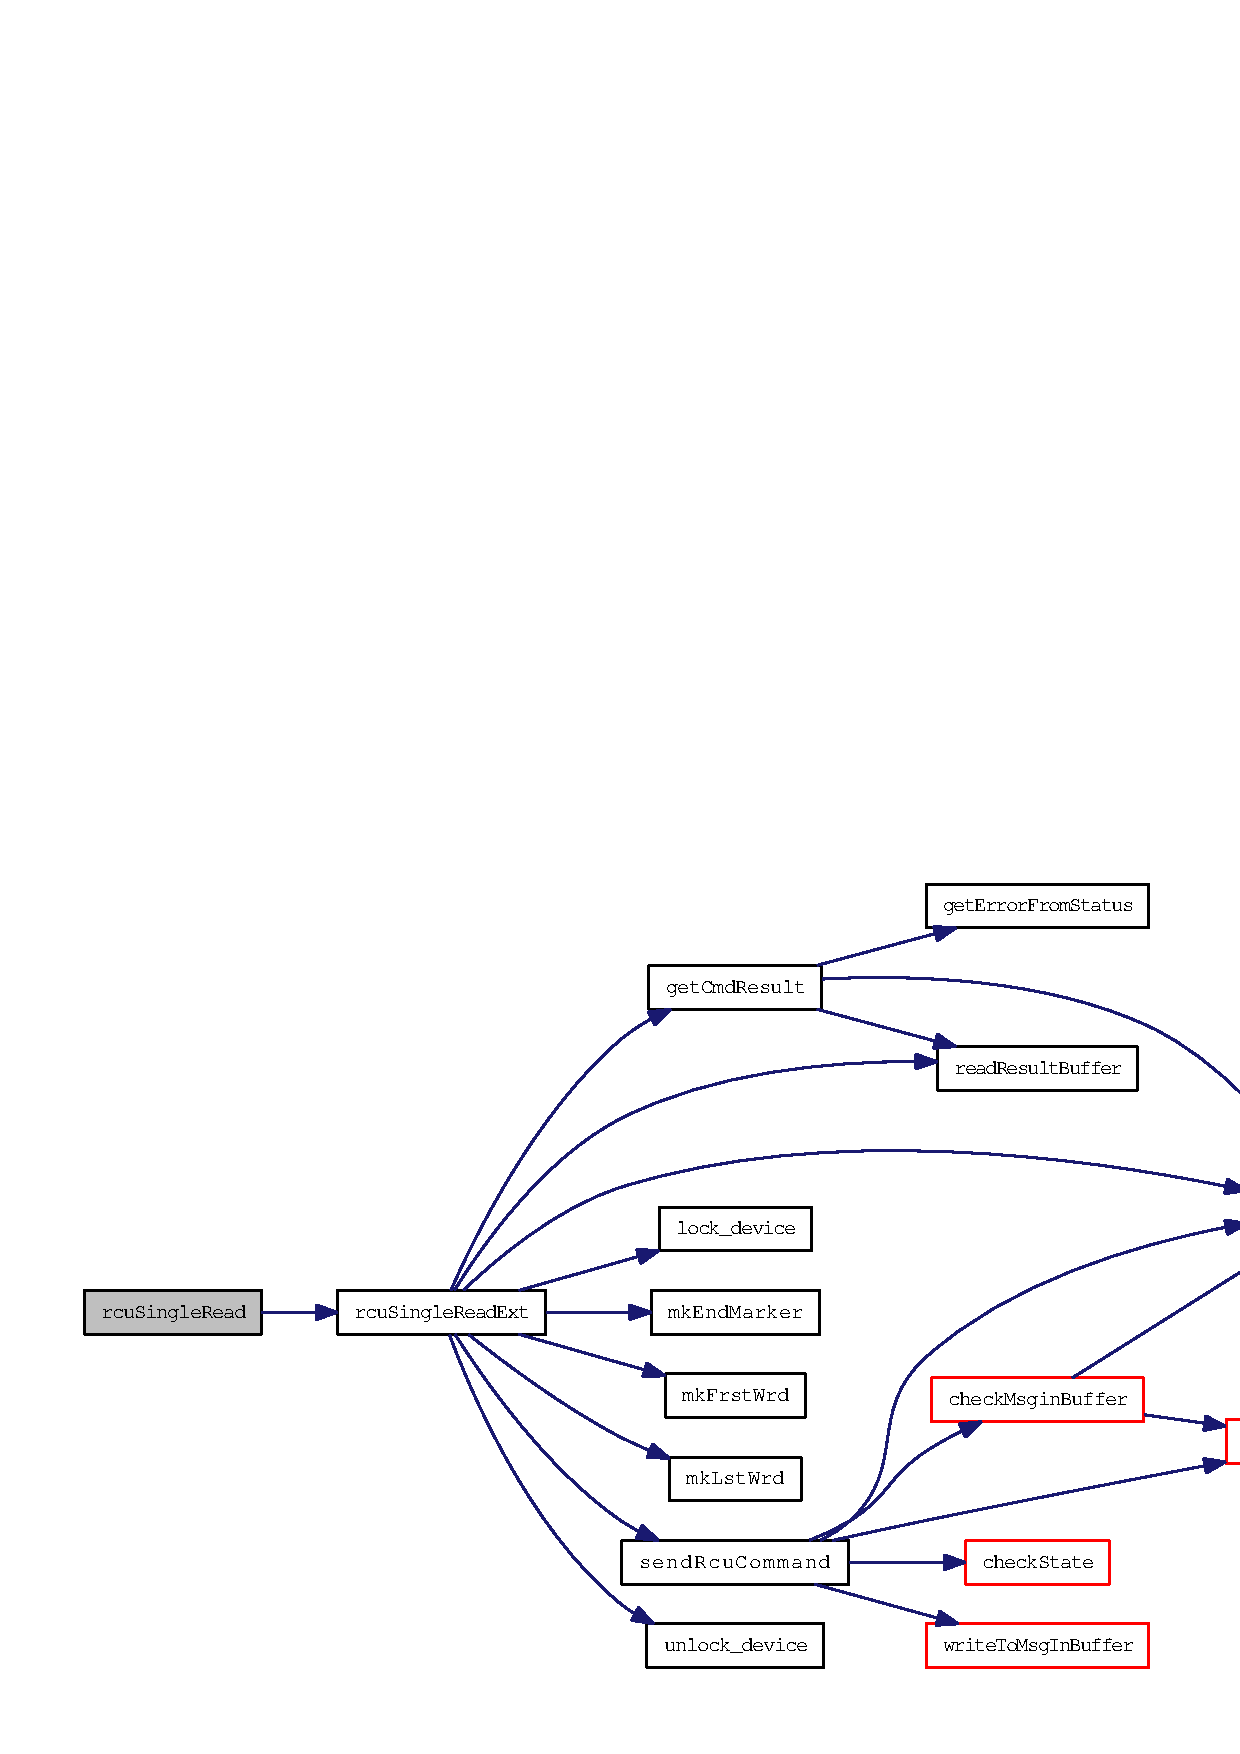
\includegraphics[width=349pt]{group__dcsc__msg__buffer__access_g339b5922513d0f0211d7962234faa24f_cgraph}
\end{center}
\end{figure}
\hypertarget{group__dcsc__msg__buffer__access_g5b2ecab6b0a6383afebde1ea486dae43}{
\index{dcsc_msg_buffer_access@{dcsc\_\-msg\_\-buffer\_\-access}!rcuSingleWrite@{rcuSingleWrite}}
\index{rcuSingleWrite@{rcuSingleWrite}!dcsc_msg_buffer_access@{dcsc\_\-msg\_\-buffer\_\-access}}
\subsubsection[rcuSingleWrite]{\setlength{\rightskip}{0pt plus 5cm}int rcu\-Single\-Write (\_\-\_\-u32 {\em address}, \_\-\_\-u32 {\em data})}}
\label{group__dcsc__msg__buffer__access_g5b2ecab6b0a6383afebde1ea486dae43}


Write a single location (32bit word). 

\begin{Desc}
\item[Parameters:]
\begin{description}
\item[{\em address}]16 bit address in RCU memory space \item[{\em data}]data word \end{description}
\end{Desc}
\begin{Desc}
\item[Returns:]\end{Desc}


Definition at line 1541 of file dcsc\-Msg\-Buffer\-Interface.c.

References MSGBUF\_\-MODE\_\-MEMMAPPED, and rcu\-Single\-Write\-Ext().

Referenced by clear\-Err\-Reg(), commit(), exec\-Write\-Cmd(), init(), main(), rcu\-Flash\-Erase(), rcu\-Flash\-ID(), rcu\-Flash\-Read(), rcu\-Flash\-Reset(), rcu\-Flash\-Write(), and step().

Here is the call graph for this function:\begin{figure}[H]
\begin{center}
\leavevmode
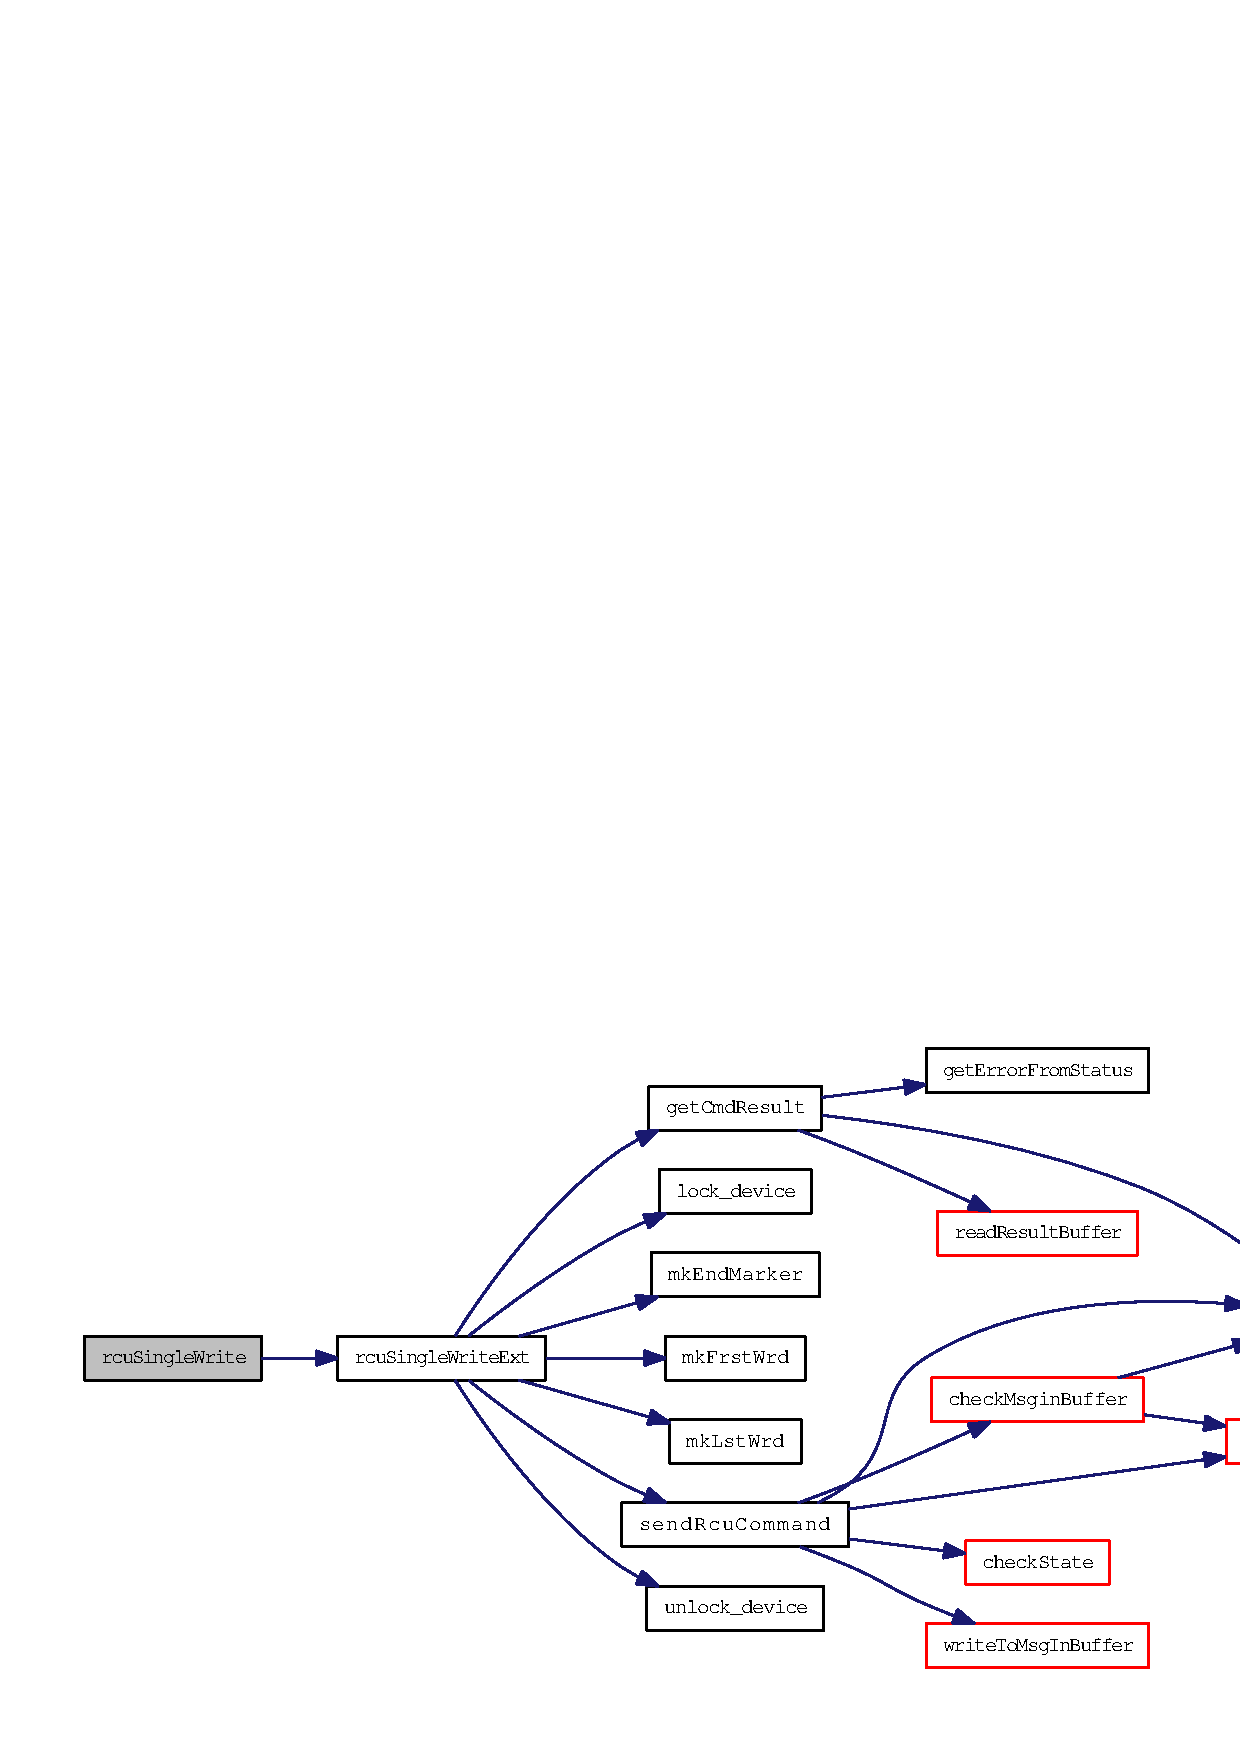
\includegraphics[width=349pt]{group__dcsc__msg__buffer__access_g5b2ecab6b0a6383afebde1ea486dae43_cgraph}
\end{center}
\end{figure}
\hypertarget{group__dcsc__msg__buffer__access_gac62a9e57c67af4cb9178b4426ec12fb}{
\index{dcsc_msg_buffer_access@{dcsc\_\-msg\_\-buffer\_\-access}!releaseRcuAccess@{releaseRcuAccess}}
\index{releaseRcuAccess@{releaseRcuAccess}!dcsc_msg_buffer_access@{dcsc\_\-msg\_\-buffer\_\-access}}
\subsubsection[releaseRcuAccess]{\setlength{\rightskip}{0pt plus 5cm}int release\-Rcu\-Access ()}}
\label{group__dcsc__msg__buffer__access_gac62a9e57c67af4cb9178b4426ec12fb}


Close the device and release internal data structures. 

\begin{Desc}
\item[Returns:]neg. error code if failed \par
 -ENXIO : no device open \end{Desc}


Definition at line 597 of file dcsc\-Msg\-Buffer\-Interface.c.

References close\-Device().

Referenced by main().

Here is the call graph for this function:\begin{figure}[H]
\begin{center}
\leavevmode
\includegraphics[width=131pt]{group__dcsc__msg__buffer__access_gac62a9e57c67af4cb9178b4426ec12fb_cgraph}
\end{center}
\end{figure}
\hypertarget{group__dcsc__msg__buffer__access_gb54d216419ff2c191363373bef5f9cfa}{
\index{dcsc_msg_buffer_access@{dcsc\_\-msg\_\-buffer\_\-access}!resetSimulation@{resetSimulation}}
\index{resetSimulation@{resetSimulation}!dcsc_msg_buffer_access@{dcsc\_\-msg\_\-buffer\_\-access}}
\subsubsection[resetSimulation]{\setlength{\rightskip}{0pt plus 5cm}void reset\-Simulation ()}}
\label{group__dcsc__msg__buffer__access_gb54d216419ff2c191363373bef5f9cfa}


Reset the simulation. 

Reset all the internal variables of the register simulation and seek to beginning of the register files. 

Definition at line 1761 of file dcsc\-Msg\-Buffer\-Interface.c.

Referenced by main(), and start\-Simulation().\hypertarget{group__dcsc__msg__buffer__access_g36bb01dae6dd6edf579fe9878f9c6a20}{
\index{dcsc_msg_buffer_access@{dcsc\_\-msg\_\-buffer\_\-access}!setDebugOptionFlag@{setDebugOptionFlag}}
\index{setDebugOptionFlag@{setDebugOptionFlag}!dcsc_msg_buffer_access@{dcsc\_\-msg\_\-buffer\_\-access}}
\subsubsection[setDebugOptionFlag]{\setlength{\rightskip}{0pt plus 5cm}int set\-Debug\-Option\-Flag (int {\em of})}}
\label{group__dcsc__msg__buffer__access_g36bb01dae6dd6edf579fe9878f9c6a20}


Set a debug option flag. 

\begin{Desc}
\item[Parameters:]
\begin{description}
\item[{\em of}]option flags \end{description}
\end{Desc}
\begin{Desc}
\item[Returns:]current value of options \end{Desc}


Definition at line 1675 of file dcsc\-Msg\-Buffer\-Interface.c.

References g\_\-options.

Referenced by build\-Data\-Buffer\-From\-File(), Convert\-ASCII2Bin(), execute\-Command\-Line(), execute\-Main\-Commands(), print\-Read\-Output\-Formatted(), Scan\-Coefficients(), and wait\-Condition().\hypertarget{group__dcsc__msg__buffer__access_gc07186b103fbe4c39531665c95e22c7e}{
\index{dcsc_msg_buffer_access@{dcsc\_\-msg\_\-buffer\_\-access}!setDebugOptions@{setDebugOptions}}
\index{setDebugOptions@{setDebugOptions}!dcsc_msg_buffer_access@{dcsc\_\-msg\_\-buffer\_\-access}}
\subsubsection[setDebugOptions]{\setlength{\rightskip}{0pt plus 5cm}int set\-Debug\-Options (int {\em options})}}
\label{group__dcsc__msg__buffer__access_gc07186b103fbe4c39531665c95e22c7e}


Set the debug options. 

Refer to the help menu. \begin{Desc}
\item[Parameters:]
\begin{description}
\item[{\em options}]debug options \end{description}
\end{Desc}
\begin{Desc}
\item[Returns:]current value of options \end{Desc}


Definition at line 1669 of file dcsc\-Msg\-Buffer\-Interface.c.

References g\_\-options.

Referenced by execute\-Main\-Commands(), and main().\hypertarget{group__dcsc__msg__buffer__access_g0adb3aacb8d7ad32ceabe66a9dcbb401}{
\index{dcsc_msg_buffer_access@{dcsc\_\-msg\_\-buffer\_\-access}!startSimulation@{startSimulation}}
\index{startSimulation@{startSimulation}!dcsc_msg_buffer_access@{dcsc\_\-msg\_\-buffer\_\-access}}
\subsubsection[startSimulation]{\setlength{\rightskip}{0pt plus 5cm}void start\-Simulation ()}}
\label{group__dcsc__msg__buffer__access_g0adb3aacb8d7ad32ceabe66a9dcbb401}


Start register simulation. 

The interface implements simulation of the firmware response for debugging purpose. Instead reading the control register (reg 0), a text file will be read. This helps when testing the software on another machine than the dcs board or when firmware is under development a comprehensive description will follow later.\par
 {\bf Note:} The simulation feature has to be turned on at configure time with the option --enable-dcscsim 

Definition at line 1779 of file dcsc\-Msg\-Buffer\-Interface.c.

References reset\-Simulation().

Referenced by main(), and wait\-Condition().

Here is the call graph for this function:\begin{figure}[H]
\begin{center}
\leavevmode
\includegraphics[width=129pt]{group__dcsc__msg__buffer__access_g0adb3aacb8d7ad32ceabe66a9dcbb401_cgraph}
\end{center}
\end{figure}
\hypertarget{group__dcsc__msg__buffer__access_gd871881385919aff64a8b679984cd018}{
\index{dcsc_msg_buffer_access@{dcsc\_\-msg\_\-buffer\_\-access}!stopSimulation@{stopSimulation}}
\index{stopSimulation@{stopSimulation}!dcsc_msg_buffer_access@{dcsc\_\-msg\_\-buffer\_\-access}}
\subsubsection[stopSimulation]{\setlength{\rightskip}{0pt plus 5cm}void stop\-Simulation ()}}
\label{group__dcsc__msg__buffer__access_gd871881385919aff64a8b679984cd018}


Stop the simulation. 

Cleanup function for the simulation feature. 

Definition at line 1800 of file dcsc\-Msg\-Buffer\-Interface.c.

Referenced by main(), and wait\-Condition().
\hypertarget{group__selectmap__access}{
\section{Selectmap Interface}
\label{group__selectmap__access}\index{Selectmap Interface@{Selectmap Interface}}
}
This module implements the basic access function to the Selectmap interface of the Xilinx FPGA on the RCU.  
\subsection*{API methods: Initialization and general methods.}
\begin{CompactItemize}
\item 
int \hyperlink{group__selectmap__access_g3a82967a2ac2933832a98aa2d822fd7b}{init\-Sm\-Access} (const char $\ast$p\-Device\-Name)
\begin{CompactList}\small\item\em Initialize the interface. \item\end{CompactList}\item 
int \hyperlink{group__selectmap__access_g75466b7556397eb41108eb84212c5b19}{release\-Sm\-Access} ()
\begin{CompactList}\small\item\em Close the device and release internal data structures. \item\end{CompactList}\end{CompactItemize}
\subsection*{Read/write access}
\begin{CompactItemize}
\item 
\_\-\_\-u32 \hyperlink{group__selectmap__access_g88f0784ea00a5707d5fc4db2778e1b2a}{sm\-Make\-T1Header} (\_\-\_\-u8 rdwr, \_\-\_\-u16 address, \_\-\_\-u16 words)
\begin{CompactList}\small\item\em Generates a Type 1 Header Package to send to the selectmap interface. \item\end{CompactList}\item 
int \hyperlink{group__selectmap__access_ge0d7561e2ddca5878fe0c39c948dfdd2}{sm\-Register\-Write} (\_\-\_\-u32 address, \_\-\_\-u32 data)
\begin{CompactList}\small\item\em Write one word to a register of the selectmap interface. \item\end{CompactList}\item 
int \hyperlink{group__selectmap__access_gf7536588344d4c30f928de00a240baa8}{sm\-Register\-Read} (\_\-\_\-u32 address, \_\-\_\-u32 $\ast$p\-Data)
\begin{CompactList}\small\item\em Read one word in a register of the selectmap interface. \item\end{CompactList}\end{CompactItemize}


\subsection{Detailed Description}
This module implements the basic access function to the Selectmap interface of the Xilinx FPGA on the RCU. 



\subsection{Function Documentation}
\hypertarget{group__selectmap__access_g3a82967a2ac2933832a98aa2d822fd7b}{
\index{selectmap_access@{selectmap\_\-access}!initSmAccess@{initSmAccess}}
\index{initSmAccess@{initSmAccess}!selectmap_access@{selectmap\_\-access}}
\subsubsection[initSmAccess]{\setlength{\rightskip}{0pt plus 5cm}int init\-Sm\-Access (const char $\ast$ {\em p\-Device\-Name})}}
\label{group__selectmap__access_g3a82967a2ac2933832a98aa2d822fd7b}


Initialize the interface. 

The device will be opened and some other other internal states initialized. \begin{Desc}
\item[Parameters:]
\begin{description}
\item[{\em p\-Device\-Name,:}]name of the device node, if NULL: /dev/rcu/virtex as default \end{description}
\end{Desc}
\begin{Desc}
\item[Returns:]neg. error code if failed\par
 -ENOSPC : can not get the size of the interface buffers, or buffers too small\par
 -ENOENT : can not open device \end{Desc}


Definition at line 43 of file selectmap\-Interface.c.

References g\_\-p\-Default\-Sm\-Device, and g\_\-Sm\-File.\hypertarget{group__selectmap__access_g75466b7556397eb41108eb84212c5b19}{
\index{selectmap_access@{selectmap\_\-access}!releaseSmAccess@{releaseSmAccess}}
\index{releaseSmAccess@{releaseSmAccess}!selectmap_access@{selectmap\_\-access}}
\subsubsection[releaseSmAccess]{\setlength{\rightskip}{0pt plus 5cm}int release\-Sm\-Access ()}}
\label{group__selectmap__access_g75466b7556397eb41108eb84212c5b19}


Close the device and release internal data structures. 

\begin{Desc}
\item[Returns:]neg. error code if failed \par
 -ENXIO : no device open \end{Desc}


Definition at line 72 of file selectmap\-Interface.c.

References g\_\-Sm\-File.

Referenced by main().\hypertarget{group__selectmap__access_g88f0784ea00a5707d5fc4db2778e1b2a}{
\index{selectmap_access@{selectmap\_\-access}!smMakeT1Header@{smMakeT1Header}}
\index{smMakeT1Header@{smMakeT1Header}!selectmap_access@{selectmap\_\-access}}
\subsubsection[smMakeT1Header]{\setlength{\rightskip}{0pt plus 5cm}\_\-\_\-u32 sm\-Make\-T1Header (\_\-\_\-u8 {\em rdwr}, \_\-\_\-u16 {\em address}, \_\-\_\-u16 {\em words})}}
\label{group__selectmap__access_g88f0784ea00a5707d5fc4db2778e1b2a}


Generates a Type 1 Header Package to send to the selectmap interface. 

\begin{Desc}
\item[Parameters:]
\begin{description}
\item[{\em rdwr}]read (1) or write (0) \item[{\em address}]address of the register \item[{\em words}]of words to read or write (max (2$^\wedge$11)-1) \end{description}
\end{Desc}
\begin{Desc}
\item[Returns:]\end{Desc}


Definition at line 80 of file selectmap\-Interface.c.

Referenced by sm\-Register\-Read(), and sm\-Register\-Write().\hypertarget{group__selectmap__access_gf7536588344d4c30f928de00a240baa8}{
\index{selectmap_access@{selectmap\_\-access}!smRegisterRead@{smRegisterRead}}
\index{smRegisterRead@{smRegisterRead}!selectmap_access@{selectmap\_\-access}}
\subsubsection[smRegisterRead]{\setlength{\rightskip}{0pt plus 5cm}int sm\-Register\-Read (\_\-\_\-u32 {\em address}, \_\-\_\-u32 $\ast$ {\em p\-Data})}}
\label{group__selectmap__access_gf7536588344d4c30f928de00a240baa8}


Read one word in a register of the selectmap interface. 

\begin{Desc}
\item[Parameters:]
\begin{description}
\item[{\em address}]register number \item[{\em p\-Data}]buffer to receive the data \end{description}
\end{Desc}
\begin{Desc}
\item[Returns:]\end{Desc}


Definition at line 148 of file selectmap\-Interface.c.

References g\_\-Sm\-File, SM\_\-REG\_\-READ, sm\-Make\-T1Header(), and VIRTEX\_\-READ\_\-REG.

Referenced by exec\-Read\-Cmd().

Here is the call graph for this function:\begin{figure}[H]
\begin{center}
\leavevmode
\includegraphics[width=138pt]{group__selectmap__access_gf7536588344d4c30f928de00a240baa8_cgraph}
\end{center}
\end{figure}
\hypertarget{group__selectmap__access_ge0d7561e2ddca5878fe0c39c948dfdd2}{
\index{selectmap_access@{selectmap\_\-access}!smRegisterWrite@{smRegisterWrite}}
\index{smRegisterWrite@{smRegisterWrite}!selectmap_access@{selectmap\_\-access}}
\subsubsection[smRegisterWrite]{\setlength{\rightskip}{0pt plus 5cm}int sm\-Register\-Write (\_\-\_\-u32 {\em address}, \_\-\_\-u32 {\em data})}}
\label{group__selectmap__access_ge0d7561e2ddca5878fe0c39c948dfdd2}


Write one word to a register of the selectmap interface. 

\begin{Desc}
\item[Parameters:]
\begin{description}
\item[{\em address}]register number \item[{\em data}]data word \end{description}
\end{Desc}
\begin{Desc}
\item[Returns:]\end{Desc}


Definition at line 135 of file selectmap\-Interface.c.

References g\_\-Sm\-File, SM\_\-REG\_\-WRITE, sm\-Make\-T1Header(), VIRTEX\_\-SET\_\-REG, and VIRTEX\_\-WRITE\_\-REG.

Referenced by exec\-Write\-Cmd().

Here is the call graph for this function:\begin{figure}[H]
\begin{center}
\leavevmode
\includegraphics[width=138pt]{group__selectmap__access_ge0d7561e2ddca5878fe0c39c948dfdd2_cgraph}
\end{center}
\end{figure}

\chapter{RCU linux tools and drivers for the DCS board Data Structure Documentation}
\hypertarget{structArgDef__t}{
\section{Arg\-Def\_\-t Struct Reference}
\label{structArgDef__t}\index{ArgDef_t@{ArgDef\_\-t}}
}
The argument definition.  


{\tt \#include $<$mrshellprim.h$>$}

Collaboration diagram for Arg\-Def\_\-t:\begin{figure}[H]
\begin{center}
\leavevmode
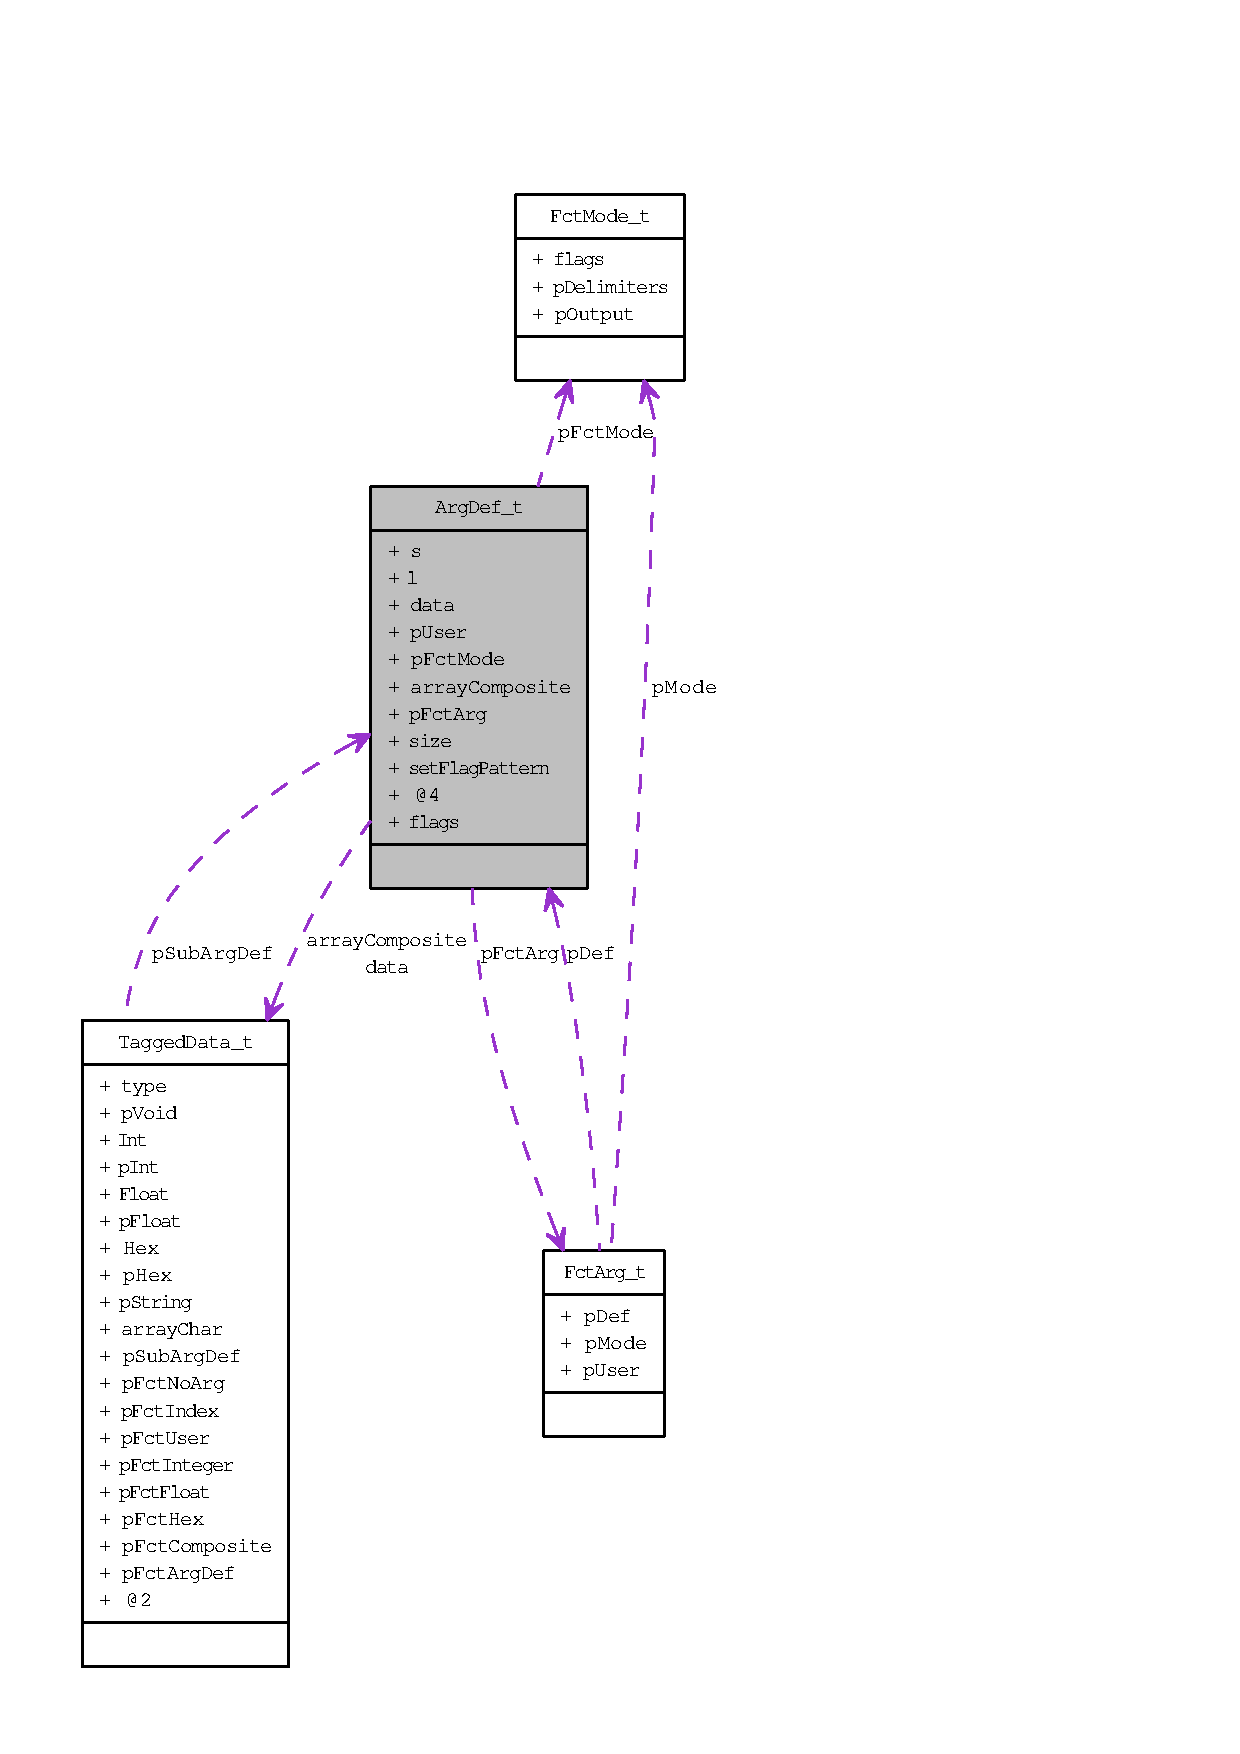
\includegraphics[width=174pt]{structArgDef__t__coll__graph}
\end{center}
\end{figure}
\subsection*{Data Fields}
\begin{CompactItemize}
\item 
const char $\ast$ \hyperlink{structArgDef__t_4ca9eeaa97d70754a94cb018d13f21cd}{s}
\begin{CompactList}\small\item\em short version of the argument \item\end{CompactList}\item 
const char $\ast$ \hyperlink{structArgDef__t_c076508155e43ccd57ed2f6c871a107d}{l}
\begin{CompactList}\small\item\em long version of the argument \item\end{CompactList}\item 
\hyperlink{structTaggedData__t}{TTagged\-Data} \hyperlink{structArgDef__t_75389251964258516f1e52fb06df857b}{data}
\begin{CompactList}\small\item\em type dependend data structure \item\end{CompactList}\item 
\begin{tabbing}
xx\=xx\=xx\=xx\=xx\=xx\=xx\=xx\=xx\=\kill
union \{\\
\>void $\ast$ \hyperlink{structArgDef__t_8705bbfe111541c0184b61a058ddccb1}{pUser}\\
\>\>{\em pointer to user defined data passed to a sub-function }\\\>\hyperlink{structFctMode__t}{TFctMode} $\ast$ \hyperlink{structArgDef__t_f0e262a888279888219539148e30391b}{pFctMode}\\
\>\>{\em mode for the next recursion }\\\>\hyperlink{structTaggedData__t}{TTaggedData} $\ast$ \hyperlink{structArgDef__t_a1d8173daa98a2ba54340e7e6a29db2e}{arrayComposite}\\
\>\hyperlink{structFctArg__t}{TFctArg} $\ast$ \hyperlink{structArgDef__t_0b8bf4785dab58cdbf9124f23cf6346f}{pFctArg}\\
\>\>\>{\em parameter to the eFctArgDef type }\\\>int \hyperlink{structArgDef__t_6dc5a1f0d48c5a90e40304930d77a0e2}{size}\\
\>\>{\em size of arrays }\\\>unsigned int \hyperlink{structArgDef__t_fbd0df81e0a7ea0c1a62a3d1e2680d14}{setFlagPattern}\\
\>\>{\em the flag pattern for the eFlag type }\\\}; \\

\end{tabbing}\begin{CompactList}\small\item\em additional type dependend data \item\end{CompactList}\item 
unsigned int \hyperlink{structArgDef__t_5b37c4058072b47e0392590c26f7d0ca}{flags}
\begin{CompactList}\small\item\em scanning flags specific to this argument \item\end{CompactList}\end{CompactItemize}


\subsection{Detailed Description}
The argument definition. 



Definition at line 285 of file mrshellprim.h.

\subsection{Field Documentation}
\hypertarget{structArgDef__t_b1edabeb6964d6bfde220a6e3f3b5374}{
\subsubsection["@4]{\setlength{\rightskip}{0pt plus 5cm}union \{ ... \} }}
\label{structArgDef__t_b1edabeb6964d6bfde220a6e3f3b5374}


additional type dependend data 

\hypertarget{structArgDef__t_a1d8173daa98a2ba54340e7e6a29db2e}{
\index{ArgDef_t@{Arg\-Def\_\-t}!arrayComposite@{arrayComposite}}
\index{arrayComposite@{arrayComposite}!ArgDef_t@{Arg\-Def\_\-t}}
\subsubsection[arrayComposite]{\setlength{\rightskip}{0pt plus 5cm}\hyperlink{structTaggedData__t}{TTagged\-Data}$\ast$ \hyperlink{structArgDef__t_a1d8173daa98a2ba54340e7e6a29db2e}{Arg\-Def\_\-t::array\-Composite}}}
\label{structArgDef__t_a1d8173daa98a2ba54340e7e6a29db2e}




Definition at line 298 of file mrshellprim.h.

Referenced by Get\-Nof\-Required\-Args().\hypertarget{structArgDef__t_75389251964258516f1e52fb06df857b}{
\index{ArgDef_t@{Arg\-Def\_\-t}!data@{data}}
\index{data@{data}!ArgDef_t@{Arg\-Def\_\-t}}
\subsubsection[data]{\setlength{\rightskip}{0pt plus 5cm}\hyperlink{structTaggedData__t}{TTagged\-Data} \hyperlink{structArgDef__t_75389251964258516f1e52fb06df857b}{Arg\-Def\_\-t::data}}}
\label{structArgDef__t_75389251964258516f1e52fb06df857b}


type dependend data structure 



Definition at line 291 of file mrshellprim.h.

Referenced by call\-Command\-Handler(), Get\-Nof\-Required\-Args(), mr\-Shell\-Prim\-Clone\-Def(), mr\-Shell\-Prim\-Get\-Data(), mr\-Shell\-Prim\-Get\-Float(), mr\-Shell\-Prim\-Get\-Hex(), mr\-Shell\-Prim\-Get\-Index(), mr\-Shell\-Prim\-Get\-Int(), mr\-Shell\-Prim\-Reset\-Volatile\-Flags(), mr\-Shell\-Prim\-Set\-Data(), Print\-Argument\-Definition(), Read\-Argument(), and Search\-Def().\hypertarget{structArgDef__t_5b37c4058072b47e0392590c26f7d0ca}{
\index{ArgDef_t@{Arg\-Def\_\-t}!flags@{flags}}
\index{flags@{flags}!ArgDef_t@{Arg\-Def\_\-t}}
\subsubsection[flags]{\setlength{\rightskip}{0pt plus 5cm}unsigned int \hyperlink{structArgDef__t_5b37c4058072b47e0392590c26f7d0ca}{Arg\-Def\_\-t::flags}}}
\label{structArgDef__t_5b37c4058072b47e0392590c26f7d0ca}


scanning flags specific to this argument 



Definition at line 307 of file mrshellprim.h.

Referenced by Scan\-Arguments(), and Search\-Def().\hypertarget{structArgDef__t_c076508155e43ccd57ed2f6c871a107d}{
\index{ArgDef_t@{Arg\-Def\_\-t}!l@{l}}
\index{l@{l}!ArgDef_t@{Arg\-Def\_\-t}}
\subsubsection[l]{\setlength{\rightskip}{0pt plus 5cm}const char$\ast$ \hyperlink{structArgDef__t_c076508155e43ccd57ed2f6c871a107d}{Arg\-Def\_\-t::l}}}
\label{structArgDef__t_c076508155e43ccd57ed2f6c871a107d}


long version of the argument 



Definition at line 289 of file mrshellprim.h.

Referenced by call\-Command\-Handler(), Scan\-Arguments(), and Search\-Def().\hypertarget{structArgDef__t_0b8bf4785dab58cdbf9124f23cf6346f}{
\index{ArgDef_t@{Arg\-Def\_\-t}!pFctArg@{pFctArg}}
\index{pFctArg@{pFctArg}!ArgDef_t@{Arg\-Def\_\-t}}
\subsubsection[pFctArg]{\setlength{\rightskip}{0pt plus 5cm}\hyperlink{structFctArg__t}{TFct\-Arg}$\ast$ \hyperlink{structArgDef__t_0b8bf4785dab58cdbf9124f23cf6346f}{Arg\-Def\_\-t::p\-Fct\-Arg}}}
\label{structArgDef__t_0b8bf4785dab58cdbf9124f23cf6346f}


parameter to the e\-Fct\-Arg\-Def type 



Definition at line 300 of file mrshellprim.h.

Referenced by call\-Command\-Handler(), and Read\-Argument().\hypertarget{structArgDef__t_f0e262a888279888219539148e30391b}{
\index{ArgDef_t@{Arg\-Def\_\-t}!pFctMode@{pFctMode}}
\index{pFctMode@{pFctMode}!ArgDef_t@{Arg\-Def\_\-t}}
\subsubsection[pFctMode]{\setlength{\rightskip}{0pt plus 5cm}\hyperlink{structFctMode__t}{TFct\-Mode}$\ast$ \hyperlink{structArgDef__t_f0e262a888279888219539148e30391b}{Arg\-Def\_\-t::p\-Fct\-Mode}}}
\label{structArgDef__t_f0e262a888279888219539148e30391b}


mode for the next recursion 



Definition at line 297 of file mrshellprim.h.

Referenced by call\-Command\-Handler().\hypertarget{structArgDef__t_8705bbfe111541c0184b61a058ddccb1}{
\index{ArgDef_t@{Arg\-Def\_\-t}!pUser@{pUser}}
\index{pUser@{pUser}!ArgDef_t@{Arg\-Def\_\-t}}
\subsubsection[pUser]{\setlength{\rightskip}{0pt plus 5cm}void$\ast$ \hyperlink{structArgDef__t_8705bbfe111541c0184b61a058ddccb1}{Arg\-Def\_\-t::p\-User}}}
\label{structArgDef__t_8705bbfe111541c0184b61a058ddccb1}


pointer to user defined data passed to a sub-function 



Definition at line 295 of file mrshellprim.h.

Referenced by call\-Command\-Handler().\hypertarget{structArgDef__t_4ca9eeaa97d70754a94cb018d13f21cd}{
\index{ArgDef_t@{Arg\-Def\_\-t}!s@{s}}
\index{s@{s}!ArgDef_t@{Arg\-Def\_\-t}}
\subsubsection[s]{\setlength{\rightskip}{0pt plus 5cm}const char$\ast$ \hyperlink{structArgDef__t_4ca9eeaa97d70754a94cb018d13f21cd}{Arg\-Def\_\-t::s}}}
\label{structArgDef__t_4ca9eeaa97d70754a94cb018d13f21cd}


short version of the argument 



Definition at line 287 of file mrshellprim.h.

Referenced by call\-Command\-Handler(), Scan\-Arguments(), and Search\-Def().\hypertarget{structArgDef__t_fbd0df81e0a7ea0c1a62a3d1e2680d14}{
\index{ArgDef_t@{Arg\-Def\_\-t}!setFlagPattern@{setFlagPattern}}
\index{setFlagPattern@{setFlagPattern}!ArgDef_t@{Arg\-Def\_\-t}}
\subsubsection[setFlagPattern]{\setlength{\rightskip}{0pt plus 5cm}unsigned int \hyperlink{structArgDef__t_fbd0df81e0a7ea0c1a62a3d1e2680d14}{Arg\-Def\_\-t::set\-Flag\-Pattern}}}
\label{structArgDef__t_fbd0df81e0a7ea0c1a62a3d1e2680d14}


the flag pattern for the e\-Flag type 



Definition at line 304 of file mrshellprim.h.

Referenced by call\-Command\-Handler().\hypertarget{structArgDef__t_6dc5a1f0d48c5a90e40304930d77a0e2}{
\index{ArgDef_t@{Arg\-Def\_\-t}!size@{size}}
\index{size@{size}!ArgDef_t@{Arg\-Def\_\-t}}
\subsubsection[size]{\setlength{\rightskip}{0pt plus 5cm}int \hyperlink{structArgDef__t_6dc5a1f0d48c5a90e40304930d77a0e2}{Arg\-Def\_\-t::size}}}
\label{structArgDef__t_6dc5a1f0d48c5a90e40304930d77a0e2}


size of arrays 



Definition at line 302 of file mrshellprim.h.

Referenced by call\-Command\-Handler(), and Get\-Nof\-Required\-Args().

The documentation for this struct was generated from the following file:\begin{CompactItemize}
\item 
\hyperlink{mrshellprim_8h}{mrshellprim.h}\end{CompactItemize}

\hypertarget{structdcscInitArguments__t}{
\section{dcsc\-Init\-Arguments\_\-t Struct Reference}
\label{structdcscInitArguments__t}\index{dcscInitArguments_t@{dcscInitArguments\_\-t}}
}
Argument struct for extended initialization.  


{\tt \#include $<$dcsc\-Msg\-Buffer\-Interface.h$>$}

\subsection*{Data Fields}
\begin{CompactItemize}
\item 
unsigned int \hyperlink{structdcscInitArguments__t_75b86ecc9df1bb76dda0c7ee0fcc4f35}{flags}
\item 
int \hyperlink{structdcscInitArguments__t_5ea3b80cc981315aa7508ba54653b57a}{i\-Verbosity}
\item 
int \hyperlink{structdcscInitArguments__t_5faecf13bfb7cb86647f13a38d37ccac}{i\-MIBSize}
\end{CompactItemize}


\subsection{Detailed Description}
Argument struct for extended initialization. 



Definition at line 308 of file dcsc\-Msg\-Buffer\-Interface.h.

\subsection{Field Documentation}
\hypertarget{structdcscInitArguments__t_75b86ecc9df1bb76dda0c7ee0fcc4f35}{
\index{dcscInitArguments_t@{dcsc\-Init\-Arguments\_\-t}!flags@{flags}}
\index{flags@{flags}!dcscInitArguments_t@{dcsc\-Init\-Arguments\_\-t}}
\subsubsection[flags]{\setlength{\rightskip}{0pt plus 5cm}unsigned int \hyperlink{structdcscInitArguments__t_75b86ecc9df1bb76dda0c7ee0fcc4f35}{dcsc\-Init\-Arguments\_\-t::flags}}}
\label{structdcscInitArguments__t_75b86ecc9df1bb76dda0c7ee0fcc4f35}




Definition at line 309 of file dcsc\-Msg\-Buffer\-Interface.h.

Referenced by init\-Rcu\-Access\-Ext(), and main().\hypertarget{structdcscInitArguments__t_5faecf13bfb7cb86647f13a38d37ccac}{
\index{dcscInitArguments_t@{dcsc\-Init\-Arguments\_\-t}!iMIBSize@{iMIBSize}}
\index{iMIBSize@{iMIBSize}!dcscInitArguments_t@{dcsc\-Init\-Arguments\_\-t}}
\subsubsection[iMIBSize]{\setlength{\rightskip}{0pt plus 5cm}int \hyperlink{structdcscInitArguments__t_5faecf13bfb7cb86647f13a38d37ccac}{dcsc\-Init\-Arguments\_\-t::i\-MIBSize}}}
\label{structdcscInitArguments__t_5faecf13bfb7cb86647f13a38d37ccac}




Definition at line 311 of file dcsc\-Msg\-Buffer\-Interface.h.

Referenced by init\-Rcu\-Access\-Ext(), and main().\hypertarget{structdcscInitArguments__t_5ea3b80cc981315aa7508ba54653b57a}{
\index{dcscInitArguments_t@{dcsc\-Init\-Arguments\_\-t}!iVerbosity@{iVerbosity}}
\index{iVerbosity@{iVerbosity}!dcscInitArguments_t@{dcsc\-Init\-Arguments\_\-t}}
\subsubsection[iVerbosity]{\setlength{\rightskip}{0pt plus 5cm}int \hyperlink{structdcscInitArguments__t_5ea3b80cc981315aa7508ba54653b57a}{dcsc\-Init\-Arguments\_\-t::i\-Verbosity}}}
\label{structdcscInitArguments__t_5ea3b80cc981315aa7508ba54653b57a}




Definition at line 310 of file dcsc\-Msg\-Buffer\-Interface.h.

Referenced by init\-Rcu\-Access\-Ext(), and main().

The documentation for this struct was generated from the following file:\begin{CompactItemize}
\item 
\hyperlink{dcscMsgBufferInterface_8h}{dcsc\-Msg\-Buffer\-Interface.h}\end{CompactItemize}

\hypertarget{structFctArg__t}{
\section{Fct\-Arg\_\-t Struct Reference}
\label{structFctArg__t}\index{FctArg_t@{FctArg\_\-t}}
}
Composite parameter to specify argument definition, scan mode and an additional user pointer for type \hyperlink{mrshellprim_8h_76a810650461f2062938ee9b82666b3607fd24779fbb8e0bc12b8241e0e436cc}{e\-Fct\-Arg\-Def}.  


{\tt \#include $<$mrshellprim.h$>$}

Collaboration diagram for Fct\-Arg\_\-t:\begin{figure}[H]
\begin{center}
\leavevmode
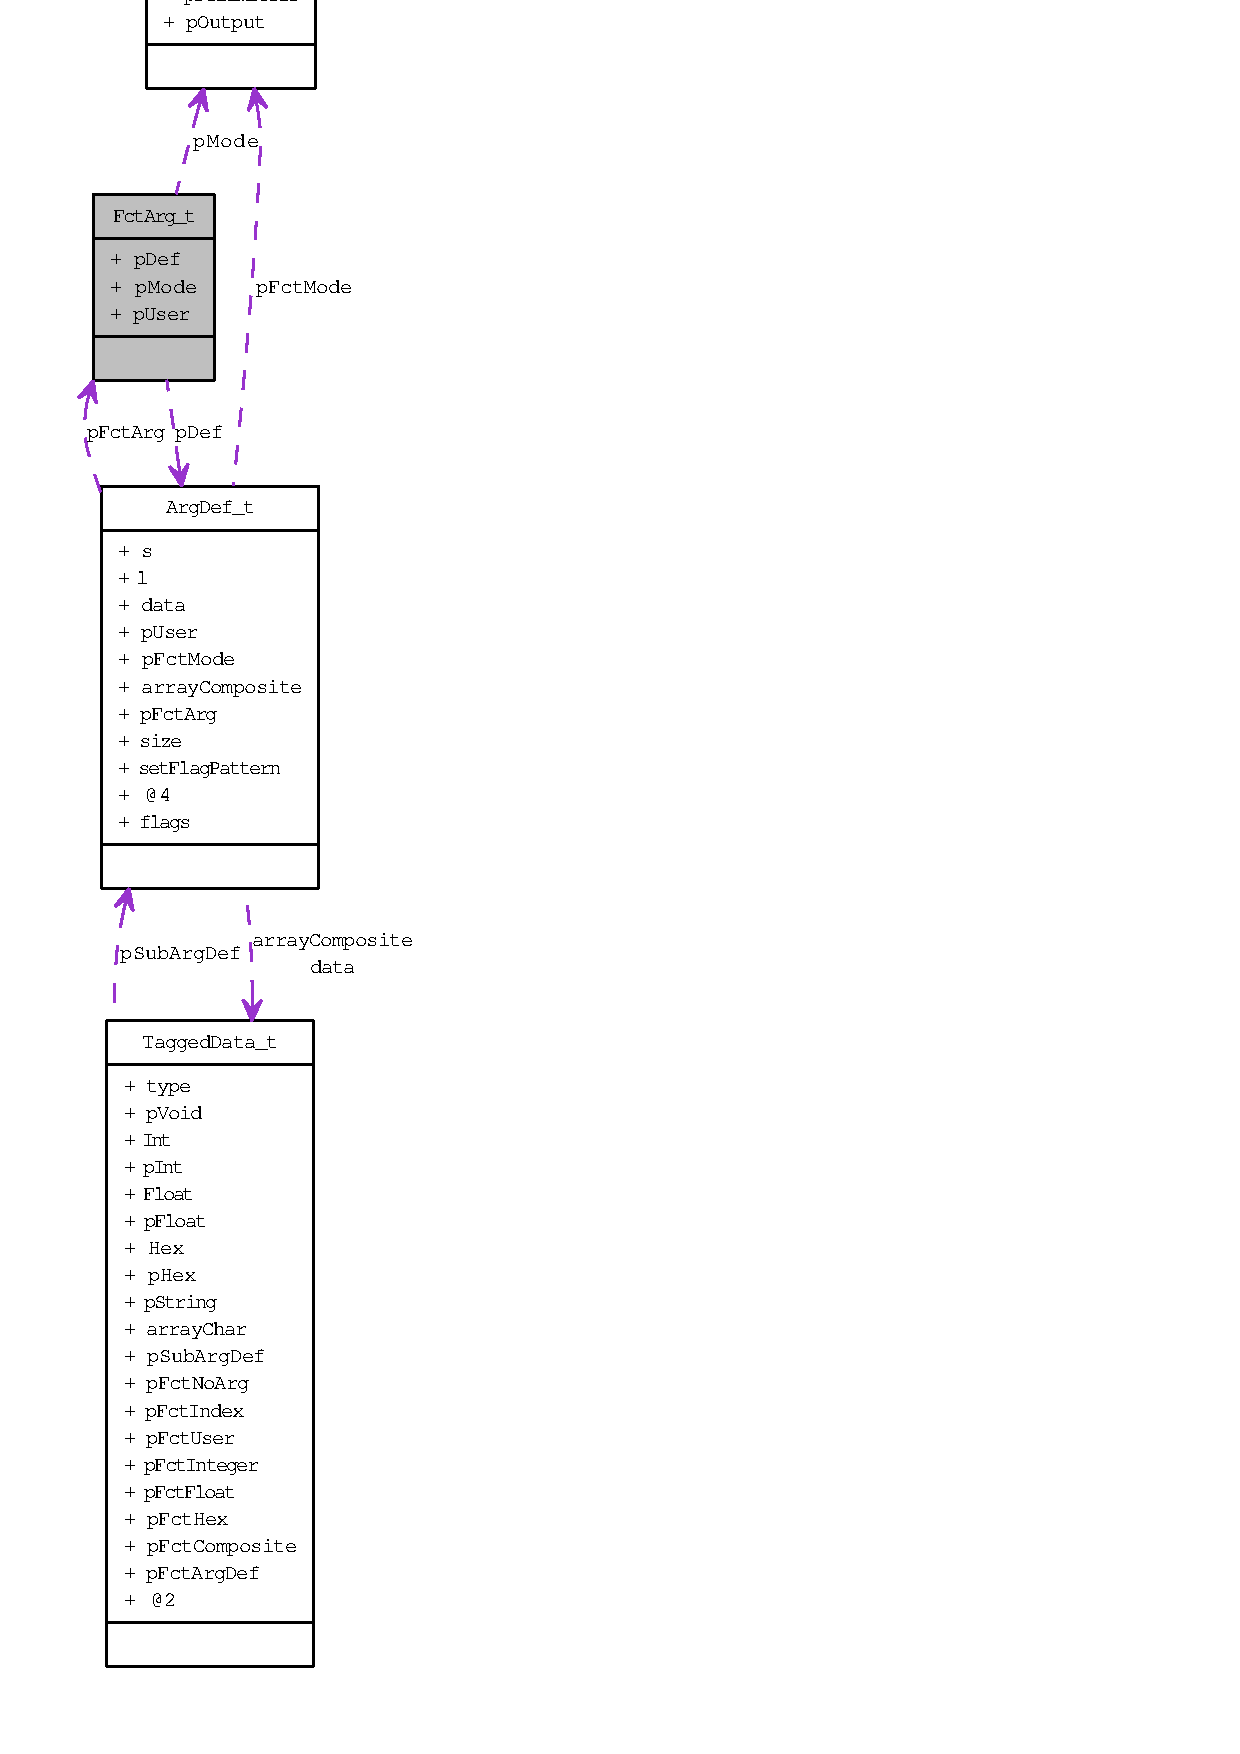
\includegraphics[width=101pt]{structFctArg__t__coll__graph}
\end{center}
\end{figure}
\subsection*{Data Fields}
\begin{CompactItemize}
\item 
\hyperlink{structArgDef__t}{TArg\-Def} $\ast$ \hyperlink{structFctArg__t_59b99d7d99fff17580f67552428c3c98}{p\-Def}
\begin{CompactList}\small\item\em the argument definition for the sub-scan \item\end{CompactList}\item 
\hyperlink{structFctMode__t}{TFct\-Mode} $\ast$ \hyperlink{structFctArg__t_b84bb7d22c66809af5f97b860c3f818e}{p\-Mode}
\begin{CompactList}\small\item\em the scanning flags for the sub-scan \item\end{CompactList}\item 
void $\ast$ \hyperlink{structFctArg__t_9369def59ef9b0c2510fe77f075c8bca}{p\-User}
\begin{CompactList}\small\item\em user pointer passed to the processing function of type \hyperlink{mrshellprim_8h_1c9f7567aaf5693ef8473ff91ccb8ff5}{Fct\-Arg\-Def} \item\end{CompactList}\end{CompactItemize}


\subsection{Detailed Description}
Composite parameter to specify argument definition, scan mode and an additional user pointer for type \hyperlink{mrshellprim_8h_76a810650461f2062938ee9b82666b3607fd24779fbb8e0bc12b8241e0e436cc}{e\-Fct\-Arg\-Def}. 



Definition at line 328 of file mrshellprim.h.

\subsection{Field Documentation}
\hypertarget{structFctArg__t_59b99d7d99fff17580f67552428c3c98}{
\index{FctArg_t@{Fct\-Arg\_\-t}!pDef@{pDef}}
\index{pDef@{pDef}!FctArg_t@{Fct\-Arg\_\-t}}
\subsubsection[pDef]{\setlength{\rightskip}{0pt plus 5cm}\hyperlink{structArgDef__t}{TArg\-Def}$\ast$ \hyperlink{structFctArg__t_59b99d7d99fff17580f67552428c3c98}{Fct\-Arg\_\-t::p\-Def}}}
\label{structFctArg__t_59b99d7d99fff17580f67552428c3c98}


the argument definition for the sub-scan 



Definition at line 330 of file mrshellprim.h.

Referenced by call\-Command\-Handler(), and Read\-Argument().\hypertarget{structFctArg__t_b84bb7d22c66809af5f97b860c3f818e}{
\index{FctArg_t@{Fct\-Arg\_\-t}!pMode@{pMode}}
\index{pMode@{pMode}!FctArg_t@{Fct\-Arg\_\-t}}
\subsubsection[pMode]{\setlength{\rightskip}{0pt plus 5cm}\hyperlink{structFctMode__t}{TFct\-Mode}$\ast$ \hyperlink{structFctArg__t_b84bb7d22c66809af5f97b860c3f818e}{Fct\-Arg\_\-t::p\-Mode}}}
\label{structFctArg__t_b84bb7d22c66809af5f97b860c3f818e}


the scanning flags for the sub-scan 



Definition at line 332 of file mrshellprim.h.

Referenced by call\-Command\-Handler(), and Read\-Argument().\hypertarget{structFctArg__t_9369def59ef9b0c2510fe77f075c8bca}{
\index{FctArg_t@{Fct\-Arg\_\-t}!pUser@{pUser}}
\index{pUser@{pUser}!FctArg_t@{Fct\-Arg\_\-t}}
\subsubsection[pUser]{\setlength{\rightskip}{0pt plus 5cm}void$\ast$ \hyperlink{structFctArg__t_9369def59ef9b0c2510fe77f075c8bca}{Fct\-Arg\_\-t::p\-User}}}
\label{structFctArg__t_9369def59ef9b0c2510fe77f075c8bca}


user pointer passed to the processing function of type \hyperlink{mrshellprim_8h_1c9f7567aaf5693ef8473ff91ccb8ff5}{Fct\-Arg\-Def} 



Definition at line 334 of file mrshellprim.h.

Referenced by call\-Command\-Handler().

The documentation for this struct was generated from the following file:\begin{CompactItemize}
\item 
\hyperlink{mrshellprim_8h}{mrshellprim.h}\end{CompactItemize}

\hypertarget{structFctMode__t}{
\section{Fct\-Mode\_\-t Struct Reference}
\label{structFctMode__t}\index{FctMode_t@{FctMode\_\-t}}
}
Composite scan mode parameter.  


{\tt \#include $<$mrshellprim.h$>$}

\subsection*{Data Fields}
\begin{CompactItemize}
\item 
unsigned int \hyperlink{structFctMode__t_d8c5e03d86fa488caeb6891156875991}{flags}
\begin{CompactList}\small\item\em global scanning flags for the current invocation of \hyperlink{mrshellprim_8h_e2735ecedc52b1199ecf8a208339c072}{Scan\-Arguments} \item\end{CompactList}\item 
const char $\ast$ \hyperlink{structFctMode__t_4b05e60cd819bcb5aa2eb72cf8764659}{p\-Delimiters}
\begin{CompactList}\small\item\em additional delimiters for arguments \item\end{CompactList}\item 
FILE $\ast$ \hyperlink{structFctMode__t_877976072dcbbc142505fb07dcb14673}{p\-Output}
\begin{CompactList}\small\item\em a file descriptor to redirect output \item\end{CompactList}\end{CompactItemize}


\subsection{Detailed Description}
Composite scan mode parameter. 



Definition at line 314 of file mrshellprim.h.

\subsection{Field Documentation}
\hypertarget{structFctMode__t_d8c5e03d86fa488caeb6891156875991}{
\index{FctMode_t@{Fct\-Mode\_\-t}!flags@{flags}}
\index{flags@{flags}!FctMode_t@{Fct\-Mode\_\-t}}
\subsubsection[flags]{\setlength{\rightskip}{0pt plus 5cm}unsigned int \hyperlink{structFctMode__t_d8c5e03d86fa488caeb6891156875991}{Fct\-Mode\_\-t::flags}}}
\label{structFctMode__t_d8c5e03d86fa488caeb6891156875991}


global scanning flags for the current invocation of \hyperlink{mrshellprim_8h_e2735ecedc52b1199ecf8a208339c072}{Scan\-Arguments} 



Definition at line 316 of file mrshellprim.h.

Referenced by Scan\-Arguments(), and Search\-Def().\hypertarget{structFctMode__t_4b05e60cd819bcb5aa2eb72cf8764659}{
\index{FctMode_t@{Fct\-Mode\_\-t}!pDelimiters@{pDelimiters}}
\index{pDelimiters@{pDelimiters}!FctMode_t@{Fct\-Mode\_\-t}}
\subsubsection[pDelimiters]{\setlength{\rightskip}{0pt plus 5cm}const char$\ast$ \hyperlink{structFctMode__t_4b05e60cd819bcb5aa2eb72cf8764659}{Fct\-Mode\_\-t::p\-Delimiters}}}
\label{structFctMode__t_4b05e60cd819bcb5aa2eb72cf8764659}


additional delimiters for arguments 



Definition at line 318 of file mrshellprim.h.

Referenced by Scan\-Arguments(), and Search\-Def().\hypertarget{structFctMode__t_877976072dcbbc142505fb07dcb14673}{
\index{FctMode_t@{Fct\-Mode\_\-t}!pOutput@{pOutput}}
\index{pOutput@{pOutput}!FctMode_t@{Fct\-Mode\_\-t}}
\subsubsection[pOutput]{\setlength{\rightskip}{0pt plus 5cm}FILE$\ast$ \hyperlink{structFctMode__t_877976072dcbbc142505fb07dcb14673}{Fct\-Mode\_\-t::p\-Output}}}
\label{structFctMode__t_877976072dcbbc142505fb07dcb14673}


a file descriptor to redirect output 



Definition at line 320 of file mrshellprim.h.

The documentation for this struct was generated from the following file:\begin{CompactItemize}
\item 
\hyperlink{mrshellprim_8h}{mrshellprim.h}\end{CompactItemize}

\hypertarget{structmsgbuf__header__t}{
\section{msgbuf\_\-header\_\-t Struct Reference}
\label{structmsgbuf__header__t}\index{msgbuf_header_t@{msgbuf\_\-header\_\-t}}
}
\subsection*{Data Fields}
\begin{CompactItemize}
\item 
int \hyperlink{structmsgbuf__header__t_2d7dc0360571deed5bb400535dd09318}{VALID\_\-FROM\_\-VERSION}
\item 
int \hyperlink{structmsgbuf__header__t_d576520bf5242643edb45474d294086b}{HEADER\_\-VERSION\_\-BITS}
\item 
int \hyperlink{structmsgbuf__header__t_0c67137e91ca9be67684094c75331f23}{HEADER\_\-VERSION\_\-BITSHIFT}
\item 
int \hyperlink{structmsgbuf__header__t_c96868f83c9b95da536f668edbb3f9db}{FRSTWORD\_\-ADD\_\-NUMWORDS}
\item 
int \hyperlink{structmsgbuf__header__t_5613d893ab652401624518811769c7f8}{FRSTWORD\_\-BITSHIFT\_\-CMDID}
\item 
int \hyperlink{structmsgbuf__header__t_10a75f96f061399a714ed5e4b37c1439}{FRSTWORD\_\-WIDTH\_\-CMDID}
\item 
int \hyperlink{structmsgbuf__header__t_8b168b71e1c62e52b43ddce2a1b777dc}{FRSTWORD\_\-BITSHIFT\_\-SFTMSG}
\item 
int \hyperlink{structmsgbuf__header__t_87b758b56e97db8198bd7d6405bdb874}{FRSTWORD\_\-WIDTH\_\-SFTMSG}
\item 
int \hyperlink{structmsgbuf__header__t_aa00d1cdea9a4385ded4fd62af6c3bd1}{FRSTWORD\_\-BITSHIFT\_\-DATAFMT}
\item 
int \hyperlink{structmsgbuf__header__t_e78c1f0a8758ef8d18056b01f664b720}{FRSTWORD\_\-WIDTH\_\-DATAFMT}
\item 
int \hyperlink{structmsgbuf__header__t_219d3f943829db1d50613a7f2629818d}{FRSTWORD\_\-BITSHIFT\_\-NUMWORDS}
\item 
int \hyperlink{structmsgbuf__header__t_45844eb2528f63b7dbd58f5947794d4b}{FRSTWORD\_\-WIDTH\_\-NUMWORDS}
\item 
int \hyperlink{structmsgbuf__header__t_51f61e787244c9002fba785687789bdb}{FRSTWORD\_\-BITSHIFT\_\-BLKNUM}
\item 
int \hyperlink{structmsgbuf__header__t_5a5421dab3b5eab22b180a8971bc9c2f}{FRSTWORD\_\-WIDTH\_\-BLKNUM}
\item 
int \hyperlink{structmsgbuf__header__t_533600b45879bd3ceca83f1f5441f7fb}{FRSTWORD\_\-BITSHIFT\_\-EXTENSION}
\item 
int \hyperlink{structmsgbuf__header__t_b43999f0c0b835ebe7e5543577e68ec9}{FRSTWORD\_\-WIDTH\_\-EXTENSION}
\item 
int \hyperlink{structmsgbuf__header__t_bbad9a4dd78f324a89fe53f5b32b18e8}{FRSTWORD\_\-BITSHIFT\_\-MODE}
\item 
int \hyperlink{structmsgbuf__header__t_427f985416682eb84096a402daf34442}{FRSTWORD\_\-WIDTH\_\-MODE}
\item 
int \hyperlink{structmsgbuf__header__t_4f6d9f143e2d0259908a2b7de3bac1b4}{MARKER\_\-PATTERN}
\item 
int \hyperlink{structmsgbuf__header__t_bb50392df1ee0c30073618c236a80174}{MARKER\_\-WIDTH}
\item 
int \hyperlink{structmsgbuf__header__t_ab81b6d9c5dfd815ff59e798ee070b0e}{MARKER\_\-BITSHIFT}
\item 
int \hyperlink{structmsgbuf__header__t_7d2334426b81bda2f4be01720f9d0e58}{ENDMARKER\_\-PATTERN}
\item 
int \hyperlink{structmsgbuf__header__t_e836817a10c51af80bd6602a6d064088}{ENDMARKER\_\-WIDTH}
\item 
int \hyperlink{structmsgbuf__header__t_ca71d6c38234c2bba52e1b6e80ef74a9}{ENDMARKER\_\-BITSHIFT}
\end{CompactItemize}


\subsection{Detailed Description}




Definition at line 84 of file dcsc\-Msg\-Buffer\-Interface.c.

\subsection{Field Documentation}
\hypertarget{structmsgbuf__header__t_ca71d6c38234c2bba52e1b6e80ef74a9}{
\index{msgbuf_header_t@{msgbuf\_\-header\_\-t}!ENDMARKER_BITSHIFT@{ENDMARKER\_\-BITSHIFT}}
\index{ENDMARKER_BITSHIFT@{ENDMARKER\_\-BITSHIFT}!msgbuf_header_t@{msgbuf\_\-header\_\-t}}
\subsubsection[ENDMARKER\_\-BITSHIFT]{\setlength{\rightskip}{0pt plus 5cm}int \hyperlink{structmsgbuf__header__t_ca71d6c38234c2bba52e1b6e80ef74a9}{msgbuf\_\-header\_\-t::ENDMARKER\_\-BITSHIFT}}}
\label{structmsgbuf__header__t_ca71d6c38234c2bba52e1b6e80ef74a9}




Definition at line 108 of file dcsc\-Msg\-Buffer\-Interface.c.

Referenced by dcsc\-Check\-Msg\-Block(), and mk\-End\-Marker().\hypertarget{structmsgbuf__header__t_7d2334426b81bda2f4be01720f9d0e58}{
\index{msgbuf_header_t@{msgbuf\_\-header\_\-t}!ENDMARKER_PATTERN@{ENDMARKER\_\-PATTERN}}
\index{ENDMARKER_PATTERN@{ENDMARKER\_\-PATTERN}!msgbuf_header_t@{msgbuf\_\-header\_\-t}}
\subsubsection[ENDMARKER\_\-PATTERN]{\setlength{\rightskip}{0pt plus 5cm}int \hyperlink{structmsgbuf__header__t_7d2334426b81bda2f4be01720f9d0e58}{msgbuf\_\-header\_\-t::ENDMARKER\_\-PATTERN}}}
\label{structmsgbuf__header__t_7d2334426b81bda2f4be01720f9d0e58}




Definition at line 106 of file dcsc\-Msg\-Buffer\-Interface.c.

Referenced by dcsc\-Check\-Msg\-Block(), and mk\-End\-Marker().\hypertarget{structmsgbuf__header__t_e836817a10c51af80bd6602a6d064088}{
\index{msgbuf_header_t@{msgbuf\_\-header\_\-t}!ENDMARKER_WIDTH@{ENDMARKER\_\-WIDTH}}
\index{ENDMARKER_WIDTH@{ENDMARKER\_\-WIDTH}!msgbuf_header_t@{msgbuf\_\-header\_\-t}}
\subsubsection[ENDMARKER\_\-WIDTH]{\setlength{\rightskip}{0pt plus 5cm}int \hyperlink{structmsgbuf__header__t_e836817a10c51af80bd6602a6d064088}{msgbuf\_\-header\_\-t::ENDMARKER\_\-WIDTH}}}
\label{structmsgbuf__header__t_e836817a10c51af80bd6602a6d064088}




Definition at line 107 of file dcsc\-Msg\-Buffer\-Interface.c.

Referenced by dcsc\-Check\-Msg\-Block().\hypertarget{structmsgbuf__header__t_c96868f83c9b95da536f668edbb3f9db}{
\index{msgbuf_header_t@{msgbuf\_\-header\_\-t}!FRSTWORD_ADD_NUMWORDS@{FRSTWORD\_\-ADD\_\-NUMWORDS}}
\index{FRSTWORD_ADD_NUMWORDS@{FRSTWORD\_\-ADD\_\-NUMWORDS}!msgbuf_header_t@{msgbuf\_\-header\_\-t}}
\subsubsection[FRSTWORD\_\-ADD\_\-NUMWORDS]{\setlength{\rightskip}{0pt plus 5cm}int \hyperlink{structmsgbuf__header__t_c96868f83c9b95da536f668edbb3f9db}{msgbuf\_\-header\_\-t::FRSTWORD\_\-ADD\_\-NUMWORDS}}}
\label{structmsgbuf__header__t_c96868f83c9b95da536f668edbb3f9db}




Definition at line 88 of file dcsc\-Msg\-Buffer\-Interface.c.

Referenced by dcsc\-Check\-Msg\-Block(), and mk\-Frst\-Wrd().\hypertarget{structmsgbuf__header__t_51f61e787244c9002fba785687789bdb}{
\index{msgbuf_header_t@{msgbuf\_\-header\_\-t}!FRSTWORD_BITSHIFT_BLKNUM@{FRSTWORD\_\-BITSHIFT\_\-BLKNUM}}
\index{FRSTWORD_BITSHIFT_BLKNUM@{FRSTWORD\_\-BITSHIFT\_\-BLKNUM}!msgbuf_header_t@{msgbuf\_\-header\_\-t}}
\subsubsection[FRSTWORD\_\-BITSHIFT\_\-BLKNUM]{\setlength{\rightskip}{0pt plus 5cm}int \hyperlink{structmsgbuf__header__t_51f61e787244c9002fba785687789bdb}{msgbuf\_\-header\_\-t::FRSTWORD\_\-BITSHIFT\_\-BLKNUM}}}
\label{structmsgbuf__header__t_51f61e787244c9002fba785687789bdb}




Definition at line 97 of file dcsc\-Msg\-Buffer\-Interface.c.

Referenced by dcsc\-Check\-Msg\-Block(), and mk\-Frst\-Wrd().\hypertarget{structmsgbuf__header__t_5613d893ab652401624518811769c7f8}{
\index{msgbuf_header_t@{msgbuf\_\-header\_\-t}!FRSTWORD_BITSHIFT_CMDID@{FRSTWORD\_\-BITSHIFT\_\-CMDID}}
\index{FRSTWORD_BITSHIFT_CMDID@{FRSTWORD\_\-BITSHIFT\_\-CMDID}!msgbuf_header_t@{msgbuf\_\-header\_\-t}}
\subsubsection[FRSTWORD\_\-BITSHIFT\_\-CMDID]{\setlength{\rightskip}{0pt plus 5cm}int \hyperlink{structmsgbuf__header__t_5613d893ab652401624518811769c7f8}{msgbuf\_\-header\_\-t::FRSTWORD\_\-BITSHIFT\_\-CMDID}}}
\label{structmsgbuf__header__t_5613d893ab652401624518811769c7f8}




Definition at line 89 of file dcsc\-Msg\-Buffer\-Interface.c.

Referenced by mk\-Frst\-Wrd().\hypertarget{structmsgbuf__header__t_aa00d1cdea9a4385ded4fd62af6c3bd1}{
\index{msgbuf_header_t@{msgbuf\_\-header\_\-t}!FRSTWORD_BITSHIFT_DATAFMT@{FRSTWORD\_\-BITSHIFT\_\-DATAFMT}}
\index{FRSTWORD_BITSHIFT_DATAFMT@{FRSTWORD\_\-BITSHIFT\_\-DATAFMT}!msgbuf_header_t@{msgbuf\_\-header\_\-t}}
\subsubsection[FRSTWORD\_\-BITSHIFT\_\-DATAFMT]{\setlength{\rightskip}{0pt plus 5cm}int \hyperlink{structmsgbuf__header__t_aa00d1cdea9a4385ded4fd62af6c3bd1}{msgbuf\_\-header\_\-t::FRSTWORD\_\-BITSHIFT\_\-DATAFMT}}}
\label{structmsgbuf__header__t_aa00d1cdea9a4385ded4fd62af6c3bd1}




Definition at line 93 of file dcsc\-Msg\-Buffer\-Interface.c.

Referenced by mk\-Frst\-Wrd().\hypertarget{structmsgbuf__header__t_533600b45879bd3ceca83f1f5441f7fb}{
\index{msgbuf_header_t@{msgbuf\_\-header\_\-t}!FRSTWORD_BITSHIFT_EXTENSION@{FRSTWORD\_\-BITSHIFT\_\-EXTENSION}}
\index{FRSTWORD_BITSHIFT_EXTENSION@{FRSTWORD\_\-BITSHIFT\_\-EXTENSION}!msgbuf_header_t@{msgbuf\_\-header\_\-t}}
\subsubsection[FRSTWORD\_\-BITSHIFT\_\-EXTENSION]{\setlength{\rightskip}{0pt plus 5cm}int \hyperlink{structmsgbuf__header__t_533600b45879bd3ceca83f1f5441f7fb}{msgbuf\_\-header\_\-t::FRSTWORD\_\-BITSHIFT\_\-EXTENSION}}}
\label{structmsgbuf__header__t_533600b45879bd3ceca83f1f5441f7fb}




Definition at line 99 of file dcsc\-Msg\-Buffer\-Interface.c.

Referenced by mk\-Frst\-Wrd().\hypertarget{structmsgbuf__header__t_bbad9a4dd78f324a89fe53f5b32b18e8}{
\index{msgbuf_header_t@{msgbuf\_\-header\_\-t}!FRSTWORD_BITSHIFT_MODE@{FRSTWORD\_\-BITSHIFT\_\-MODE}}
\index{FRSTWORD_BITSHIFT_MODE@{FRSTWORD\_\-BITSHIFT\_\-MODE}!msgbuf_header_t@{msgbuf\_\-header\_\-t}}
\subsubsection[FRSTWORD\_\-BITSHIFT\_\-MODE]{\setlength{\rightskip}{0pt plus 5cm}int \hyperlink{structmsgbuf__header__t_bbad9a4dd78f324a89fe53f5b32b18e8}{msgbuf\_\-header\_\-t::FRSTWORD\_\-BITSHIFT\_\-MODE}}}
\label{structmsgbuf__header__t_bbad9a4dd78f324a89fe53f5b32b18e8}




Definition at line 101 of file dcsc\-Msg\-Buffer\-Interface.c.

Referenced by mk\-Frst\-Wrd(), and send\-Rcu\-Command().\hypertarget{structmsgbuf__header__t_219d3f943829db1d50613a7f2629818d}{
\index{msgbuf_header_t@{msgbuf\_\-header\_\-t}!FRSTWORD_BITSHIFT_NUMWORDS@{FRSTWORD\_\-BITSHIFT\_\-NUMWORDS}}
\index{FRSTWORD_BITSHIFT_NUMWORDS@{FRSTWORD\_\-BITSHIFT\_\-NUMWORDS}!msgbuf_header_t@{msgbuf\_\-header\_\-t}}
\subsubsection[FRSTWORD\_\-BITSHIFT\_\-NUMWORDS]{\setlength{\rightskip}{0pt plus 5cm}int \hyperlink{structmsgbuf__header__t_219d3f943829db1d50613a7f2629818d}{msgbuf\_\-header\_\-t::FRSTWORD\_\-BITSHIFT\_\-NUMWORDS}}}
\label{structmsgbuf__header__t_219d3f943829db1d50613a7f2629818d}




Definition at line 95 of file dcsc\-Msg\-Buffer\-Interface.c.

Referenced by dcsc\-Check\-Msg\-Block(), and mk\-Frst\-Wrd().\hypertarget{structmsgbuf__header__t_8b168b71e1c62e52b43ddce2a1b777dc}{
\index{msgbuf_header_t@{msgbuf\_\-header\_\-t}!FRSTWORD_BITSHIFT_SFTMSG@{FRSTWORD\_\-BITSHIFT\_\-SFTMSG}}
\index{FRSTWORD_BITSHIFT_SFTMSG@{FRSTWORD\_\-BITSHIFT\_\-SFTMSG}!msgbuf_header_t@{msgbuf\_\-header\_\-t}}
\subsubsection[FRSTWORD\_\-BITSHIFT\_\-SFTMSG]{\setlength{\rightskip}{0pt plus 5cm}int \hyperlink{structmsgbuf__header__t_8b168b71e1c62e52b43ddce2a1b777dc}{msgbuf\_\-header\_\-t::FRSTWORD\_\-BITSHIFT\_\-SFTMSG}}}
\label{structmsgbuf__header__t_8b168b71e1c62e52b43ddce2a1b777dc}




Definition at line 91 of file dcsc\-Msg\-Buffer\-Interface.c.\hypertarget{structmsgbuf__header__t_5a5421dab3b5eab22b180a8971bc9c2f}{
\index{msgbuf_header_t@{msgbuf\_\-header\_\-t}!FRSTWORD_WIDTH_BLKNUM@{FRSTWORD\_\-WIDTH\_\-BLKNUM}}
\index{FRSTWORD_WIDTH_BLKNUM@{FRSTWORD\_\-WIDTH\_\-BLKNUM}!msgbuf_header_t@{msgbuf\_\-header\_\-t}}
\subsubsection[FRSTWORD\_\-WIDTH\_\-BLKNUM]{\setlength{\rightskip}{0pt plus 5cm}int \hyperlink{structmsgbuf__header__t_5a5421dab3b5eab22b180a8971bc9c2f}{msgbuf\_\-header\_\-t::FRSTWORD\_\-WIDTH\_\-BLKNUM}}}
\label{structmsgbuf__header__t_5a5421dab3b5eab22b180a8971bc9c2f}




Definition at line 98 of file dcsc\-Msg\-Buffer\-Interface.c.

Referenced by dcsc\-Check\-Msg\-Block(), and mk\-Frst\-Wrd().\hypertarget{structmsgbuf__header__t_10a75f96f061399a714ed5e4b37c1439}{
\index{msgbuf_header_t@{msgbuf\_\-header\_\-t}!FRSTWORD_WIDTH_CMDID@{FRSTWORD\_\-WIDTH\_\-CMDID}}
\index{FRSTWORD_WIDTH_CMDID@{FRSTWORD\_\-WIDTH\_\-CMDID}!msgbuf_header_t@{msgbuf\_\-header\_\-t}}
\subsubsection[FRSTWORD\_\-WIDTH\_\-CMDID]{\setlength{\rightskip}{0pt plus 5cm}int \hyperlink{structmsgbuf__header__t_10a75f96f061399a714ed5e4b37c1439}{msgbuf\_\-header\_\-t::FRSTWORD\_\-WIDTH\_\-CMDID}}}
\label{structmsgbuf__header__t_10a75f96f061399a714ed5e4b37c1439}




Definition at line 90 of file dcsc\-Msg\-Buffer\-Interface.c.

Referenced by mk\-Frst\-Wrd().\hypertarget{structmsgbuf__header__t_e78c1f0a8758ef8d18056b01f664b720}{
\index{msgbuf_header_t@{msgbuf\_\-header\_\-t}!FRSTWORD_WIDTH_DATAFMT@{FRSTWORD\_\-WIDTH\_\-DATAFMT}}
\index{FRSTWORD_WIDTH_DATAFMT@{FRSTWORD\_\-WIDTH\_\-DATAFMT}!msgbuf_header_t@{msgbuf\_\-header\_\-t}}
\subsubsection[FRSTWORD\_\-WIDTH\_\-DATAFMT]{\setlength{\rightskip}{0pt plus 5cm}int \hyperlink{structmsgbuf__header__t_e78c1f0a8758ef8d18056b01f664b720}{msgbuf\_\-header\_\-t::FRSTWORD\_\-WIDTH\_\-DATAFMT}}}
\label{structmsgbuf__header__t_e78c1f0a8758ef8d18056b01f664b720}




Definition at line 94 of file dcsc\-Msg\-Buffer\-Interface.c.

Referenced by mk\-Frst\-Wrd().\hypertarget{structmsgbuf__header__t_b43999f0c0b835ebe7e5543577e68ec9}{
\index{msgbuf_header_t@{msgbuf\_\-header\_\-t}!FRSTWORD_WIDTH_EXTENSION@{FRSTWORD\_\-WIDTH\_\-EXTENSION}}
\index{FRSTWORD_WIDTH_EXTENSION@{FRSTWORD\_\-WIDTH\_\-EXTENSION}!msgbuf_header_t@{msgbuf\_\-header\_\-t}}
\subsubsection[FRSTWORD\_\-WIDTH\_\-EXTENSION]{\setlength{\rightskip}{0pt plus 5cm}int \hyperlink{structmsgbuf__header__t_b43999f0c0b835ebe7e5543577e68ec9}{msgbuf\_\-header\_\-t::FRSTWORD\_\-WIDTH\_\-EXTENSION}}}
\label{structmsgbuf__header__t_b43999f0c0b835ebe7e5543577e68ec9}




Definition at line 100 of file dcsc\-Msg\-Buffer\-Interface.c.

Referenced by mk\-Frst\-Wrd().\hypertarget{structmsgbuf__header__t_427f985416682eb84096a402daf34442}{
\index{msgbuf_header_t@{msgbuf\_\-header\_\-t}!FRSTWORD_WIDTH_MODE@{FRSTWORD\_\-WIDTH\_\-MODE}}
\index{FRSTWORD_WIDTH_MODE@{FRSTWORD\_\-WIDTH\_\-MODE}!msgbuf_header_t@{msgbuf\_\-header\_\-t}}
\subsubsection[FRSTWORD\_\-WIDTH\_\-MODE]{\setlength{\rightskip}{0pt plus 5cm}int \hyperlink{structmsgbuf__header__t_427f985416682eb84096a402daf34442}{msgbuf\_\-header\_\-t::FRSTWORD\_\-WIDTH\_\-MODE}}}
\label{structmsgbuf__header__t_427f985416682eb84096a402daf34442}




Definition at line 102 of file dcsc\-Msg\-Buffer\-Interface.c.

Referenced by mk\-Frst\-Wrd(), and send\-Rcu\-Command().\hypertarget{structmsgbuf__header__t_45844eb2528f63b7dbd58f5947794d4b}{
\index{msgbuf_header_t@{msgbuf\_\-header\_\-t}!FRSTWORD_WIDTH_NUMWORDS@{FRSTWORD\_\-WIDTH\_\-NUMWORDS}}
\index{FRSTWORD_WIDTH_NUMWORDS@{FRSTWORD\_\-WIDTH\_\-NUMWORDS}!msgbuf_header_t@{msgbuf\_\-header\_\-t}}
\subsubsection[FRSTWORD\_\-WIDTH\_\-NUMWORDS]{\setlength{\rightskip}{0pt plus 5cm}int \hyperlink{structmsgbuf__header__t_45844eb2528f63b7dbd58f5947794d4b}{msgbuf\_\-header\_\-t::FRSTWORD\_\-WIDTH\_\-NUMWORDS}}}
\label{structmsgbuf__header__t_45844eb2528f63b7dbd58f5947794d4b}




Definition at line 96 of file dcsc\-Msg\-Buffer\-Interface.c.

Referenced by dcsc\-Check\-Msg\-Block(), and mk\-Frst\-Wrd().\hypertarget{structmsgbuf__header__t_87b758b56e97db8198bd7d6405bdb874}{
\index{msgbuf_header_t@{msgbuf\_\-header\_\-t}!FRSTWORD_WIDTH_SFTMSG@{FRSTWORD\_\-WIDTH\_\-SFTMSG}}
\index{FRSTWORD_WIDTH_SFTMSG@{FRSTWORD\_\-WIDTH\_\-SFTMSG}!msgbuf_header_t@{msgbuf\_\-header\_\-t}}
\subsubsection[FRSTWORD\_\-WIDTH\_\-SFTMSG]{\setlength{\rightskip}{0pt plus 5cm}int \hyperlink{structmsgbuf__header__t_87b758b56e97db8198bd7d6405bdb874}{msgbuf\_\-header\_\-t::FRSTWORD\_\-WIDTH\_\-SFTMSG}}}
\label{structmsgbuf__header__t_87b758b56e97db8198bd7d6405bdb874}




Definition at line 92 of file dcsc\-Msg\-Buffer\-Interface.c.\hypertarget{structmsgbuf__header__t_d576520bf5242643edb45474d294086b}{
\index{msgbuf_header_t@{msgbuf\_\-header\_\-t}!HEADER_VERSION_BITS@{HEADER\_\-VERSION\_\-BITS}}
\index{HEADER_VERSION_BITS@{HEADER\_\-VERSION\_\-BITS}!msgbuf_header_t@{msgbuf\_\-header\_\-t}}
\subsubsection[HEADER\_\-VERSION\_\-BITS]{\setlength{\rightskip}{0pt plus 5cm}int \hyperlink{structmsgbuf__header__t_d576520bf5242643edb45474d294086b}{msgbuf\_\-header\_\-t::HEADER\_\-VERSION\_\-BITS}}}
\label{structmsgbuf__header__t_d576520bf5242643edb45474d294086b}




Definition at line 86 of file dcsc\-Msg\-Buffer\-Interface.c.

Referenced by mk\-Frst\-Wrd().\hypertarget{structmsgbuf__header__t_0c67137e91ca9be67684094c75331f23}{
\index{msgbuf_header_t@{msgbuf\_\-header\_\-t}!HEADER_VERSION_BITSHIFT@{HEADER\_\-VERSION\_\-BITSHIFT}}
\index{HEADER_VERSION_BITSHIFT@{HEADER\_\-VERSION\_\-BITSHIFT}!msgbuf_header_t@{msgbuf\_\-header\_\-t}}
\subsubsection[HEADER\_\-VERSION\_\-BITSHIFT]{\setlength{\rightskip}{0pt plus 5cm}int \hyperlink{structmsgbuf__header__t_0c67137e91ca9be67684094c75331f23}{msgbuf\_\-header\_\-t::HEADER\_\-VERSION\_\-BITSHIFT}}}
\label{structmsgbuf__header__t_0c67137e91ca9be67684094c75331f23}




Definition at line 87 of file dcsc\-Msg\-Buffer\-Interface.c.

Referenced by mk\-Frst\-Wrd().\hypertarget{structmsgbuf__header__t_ab81b6d9c5dfd815ff59e798ee070b0e}{
\index{msgbuf_header_t@{msgbuf\_\-header\_\-t}!MARKER_BITSHIFT@{MARKER\_\-BITSHIFT}}
\index{MARKER_BITSHIFT@{MARKER\_\-BITSHIFT}!msgbuf_header_t@{msgbuf\_\-header\_\-t}}
\subsubsection[MARKER\_\-BITSHIFT]{\setlength{\rightskip}{0pt plus 5cm}int \hyperlink{structmsgbuf__header__t_ab81b6d9c5dfd815ff59e798ee070b0e}{msgbuf\_\-header\_\-t::MARKER\_\-BITSHIFT}}}
\label{structmsgbuf__header__t_ab81b6d9c5dfd815ff59e798ee070b0e}




Definition at line 105 of file dcsc\-Msg\-Buffer\-Interface.c.

Referenced by dcsc\-Check\-Msg\-Block(), and mk\-Lst\-Wrd().\hypertarget{structmsgbuf__header__t_4f6d9f143e2d0259908a2b7de3bac1b4}{
\index{msgbuf_header_t@{msgbuf\_\-header\_\-t}!MARKER_PATTERN@{MARKER\_\-PATTERN}}
\index{MARKER_PATTERN@{MARKER\_\-PATTERN}!msgbuf_header_t@{msgbuf\_\-header\_\-t}}
\subsubsection[MARKER\_\-PATTERN]{\setlength{\rightskip}{0pt plus 5cm}int \hyperlink{structmsgbuf__header__t_4f6d9f143e2d0259908a2b7de3bac1b4}{msgbuf\_\-header\_\-t::MARKER\_\-PATTERN}}}
\label{structmsgbuf__header__t_4f6d9f143e2d0259908a2b7de3bac1b4}




Definition at line 103 of file dcsc\-Msg\-Buffer\-Interface.c.

Referenced by dcsc\-Check\-Msg\-Block(), and mk\-Lst\-Wrd().\hypertarget{structmsgbuf__header__t_bb50392df1ee0c30073618c236a80174}{
\index{msgbuf_header_t@{msgbuf\_\-header\_\-t}!MARKER_WIDTH@{MARKER\_\-WIDTH}}
\index{MARKER_WIDTH@{MARKER\_\-WIDTH}!msgbuf_header_t@{msgbuf\_\-header\_\-t}}
\subsubsection[MARKER\_\-WIDTH]{\setlength{\rightskip}{0pt plus 5cm}int \hyperlink{structmsgbuf__header__t_bb50392df1ee0c30073618c236a80174}{msgbuf\_\-header\_\-t::MARKER\_\-WIDTH}}}
\label{structmsgbuf__header__t_bb50392df1ee0c30073618c236a80174}




Definition at line 104 of file dcsc\-Msg\-Buffer\-Interface.c.

Referenced by dcsc\-Check\-Msg\-Block().\hypertarget{structmsgbuf__header__t_2d7dc0360571deed5bb400535dd09318}{
\index{msgbuf_header_t@{msgbuf\_\-header\_\-t}!VALID_FROM_VERSION@{VALID\_\-FROM\_\-VERSION}}
\index{VALID_FROM_VERSION@{VALID\_\-FROM\_\-VERSION}!msgbuf_header_t@{msgbuf\_\-header\_\-t}}
\subsubsection[VALID\_\-FROM\_\-VERSION]{\setlength{\rightskip}{0pt plus 5cm}int \hyperlink{structmsgbuf__header__t_2d7dc0360571deed5bb400535dd09318}{msgbuf\_\-header\_\-t::VALID\_\-FROM\_\-VERSION}}}
\label{structmsgbuf__header__t_2d7dc0360571deed5bb400535dd09318}




Definition at line 85 of file dcsc\-Msg\-Buffer\-Interface.c.

Referenced by open\-Device().

The documentation for this struct was generated from the following file:\begin{CompactItemize}
\item 
\hyperlink{dcscMsgBufferInterface_8c}{dcsc\-Msg\-Buffer\-Interface.c}\end{CompactItemize}

\hypertarget{structTaggedData__t}{
\section{Tagged\-Data\_\-t Struct Reference}
\label{structTaggedData__t}\index{TaggedData_t@{TaggedData\_\-t}}
}
Named Data elements to be specified as target in an argument definition \hyperlink{structArgDef__t}{Arg\-Def\_\-t}.  


{\tt \#include $<$mrshellprim.h$>$}

Collaboration diagram for Tagged\-Data\_\-t:\begin{figure}[H]
\begin{center}
\leavevmode
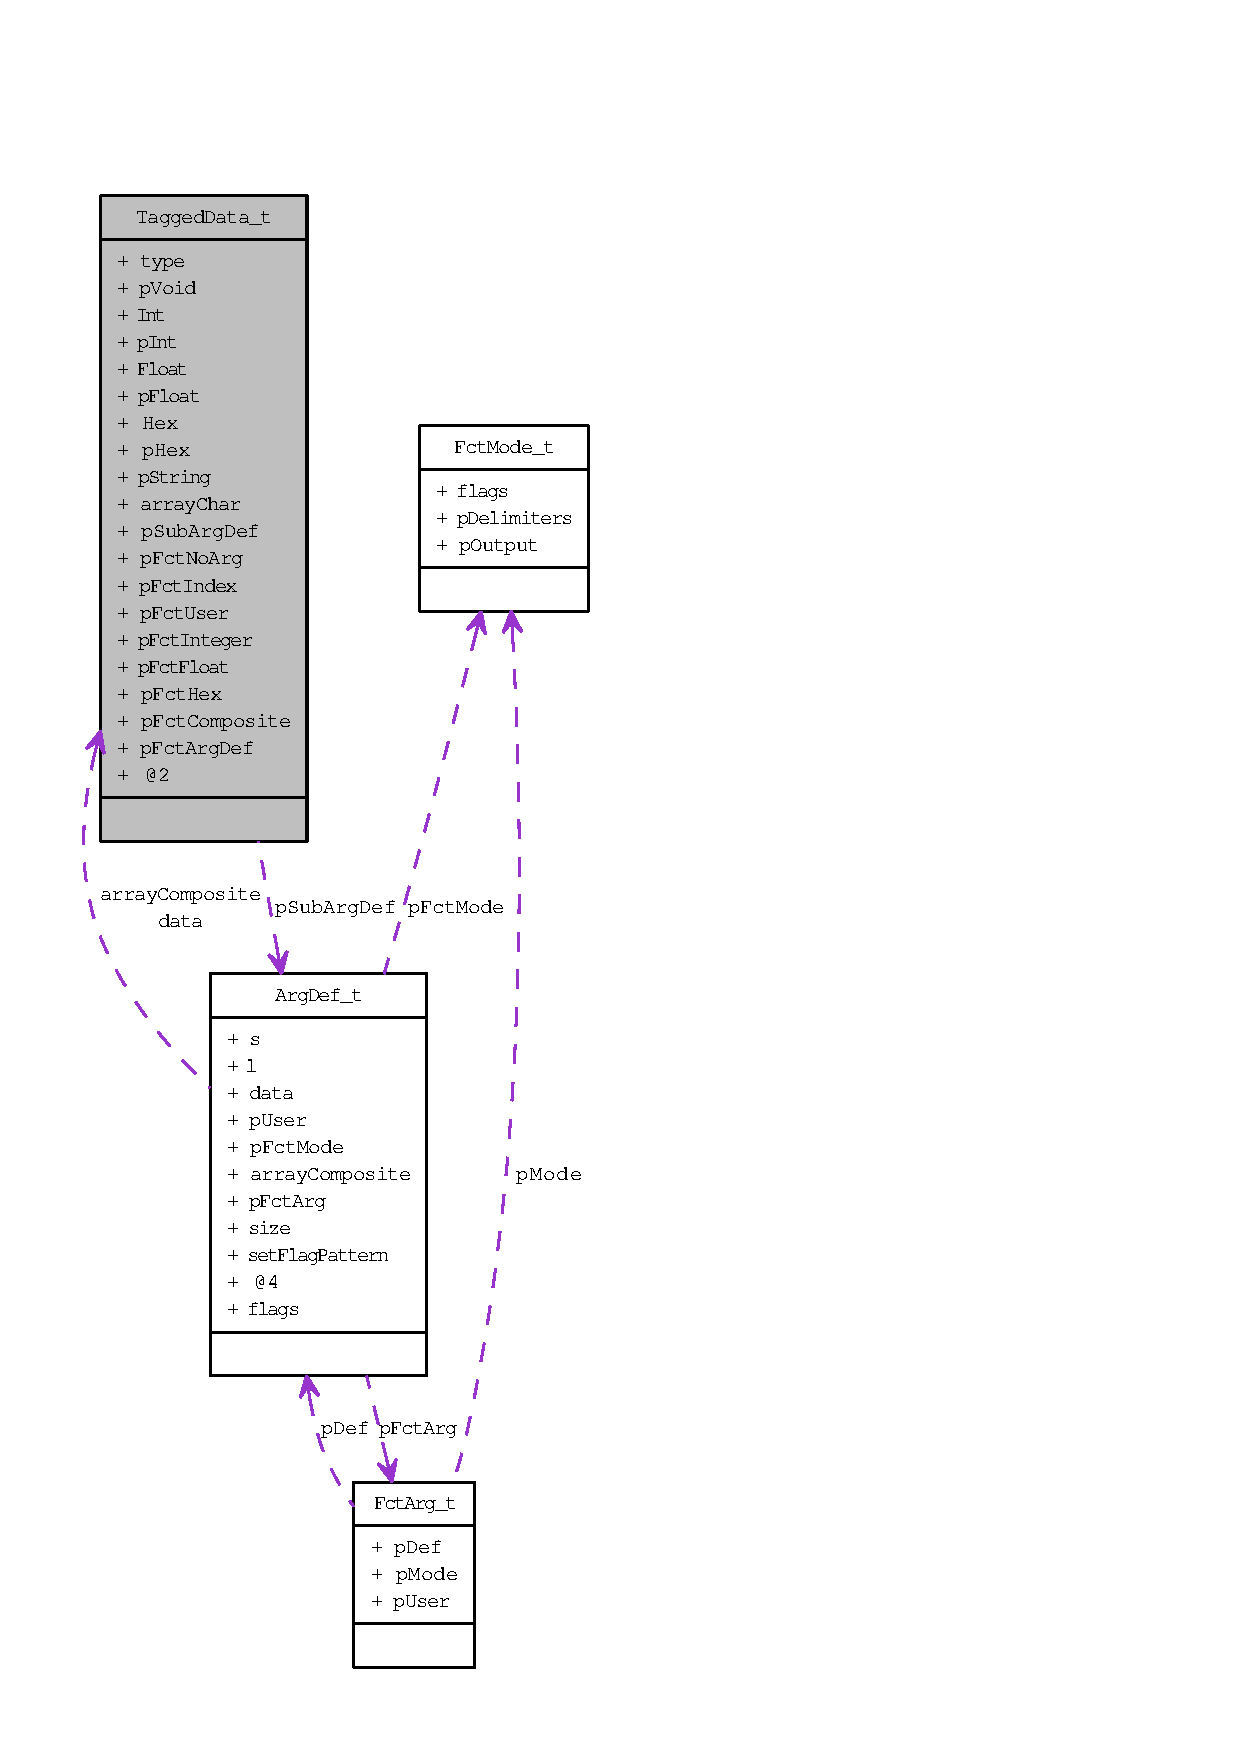
\includegraphics[width=143pt]{structTaggedData__t__coll__graph}
\end{center}
\end{figure}
\subsection*{Data Fields}
\begin{CompactItemize}
\item 
int \hyperlink{structTaggedData__t_d577c1ca9cfb883e8f61383aee2eb9b4}{type}
\begin{CompactList}\small\item\em type of the data pointer \item\end{CompactList}\item 
\begin{tabbing}
xx\=xx\=xx\=xx\=xx\=xx\=xx\=xx\=xx\=\kill
union \{\\
\>void $\ast$ \hyperlink{structTaggedData__t_5aa3ac9b92e687fc48272ced2ec2f662}{pVoid}\\
\>\>{\em void pointer element }\\\>int \hyperlink{structTaggedData__t_bd711fd71d65cb2aa3f10d8e6793707d}{Int}\\
\>\>{\em int element for types \hyperlink{mrshellprim_8h_76a810650461f2062938ee9b82666b36dd647739976fe8f17c25e3fe04d30eeb}{eInteger} and \hyperlink{mrshellprim_8h_76a810650461f2062938ee9b82666b365461a9e2704387e11258e14a0b41ac1a}{eBool} }\\\>int $\ast$ \hyperlink{structTaggedData__t_d3d58b0a67cc759b746654b7b9d09ae5}{pInt}\\
\>\>{\em int array element for types \hyperlink{mrshellprim_8h_76a810650461f2062938ee9b82666b36f56ebbf9f6232a573f846cffa9f914e9}{eIntegerArray} and \hyperlink{mrshellprim_8h_76a810650461f2062938ee9b82666b36514baa0f6ca7bbfba804b8826c13cffb}{eFlag} }\\\>float \hyperlink{structTaggedData__t_a7851afd8e427802c7fa7a2d7b9651dd}{Float}\\
\>\>{\em float element for type \hyperlink{mrshellprim_8h_76a810650461f2062938ee9b82666b364a5cba5eee27b47a9cf3714e4db4206d}{eFloat} }\\\>float $\ast$ \hyperlink{structTaggedData__t_6315613fa330301fc9be1da20c50c352}{pFloat}\\
\>\>{\em float array element for type \hyperlink{mrshellprim_8h_76a810650461f2062938ee9b82666b361cf54b260432a1baf68bed16081357c7}{eFloatArray} }\\\>unsigned int \hyperlink{structTaggedData__t_fb6384a765e6dec1e70a7044d44cfbb5}{Hex}\\
\>\>{\em uint element for type \hyperlink{mrshellprim_8h_76a810650461f2062938ee9b82666b36a64d04be3dc94180a329fac904a5d239}{eHex} }\\\>unsigned int $\ast$ \hyperlink{structTaggedData__t_7128a4892c178f6ab61b642e46b72720}{pHex}\\
\>\>{\em uint array element for type \hyperlink{mrshellprim_8h_76a810650461f2062938ee9b82666b36be303c42da892f2d0101b668e8aa252a}{eHexArray} }\\\>const char $\ast$ \hyperlink{structTaggedData__t_3ec8155fed9da63b73d80c0ef41ab2a4}{pString}\\
\>\>{\em target for type \hyperlink{mrshellprim_8h_76a810650461f2062938ee9b82666b369bf242e7bb183d9518928958c83c9a22}{eConstString} }\\\>char $\ast$ \hyperlink{structTaggedData__t_e7f993fc307df08808cd7aff4962f656}{arrayChar}\\
\>\>{\em target for type \hyperlink{mrshellprim_8h_76a810650461f2062938ee9b82666b360a10a6c7f681516162b85d6096fc394e}{eCharArray} }\\\>\hyperlink{structArgDef__t}{TArgDef} $\ast$ \hyperlink{structTaggedData__t_efbba58fc516f932be799255c9b5e119}{pSubArgDef}\\
\>\>{\em processing function for types \hyperlink{mrshellprim_8h_76a810650461f2062938ee9b82666b36b36d09249e94b5aa513d0aa3c7aa08c8}{eFctRemaining} and \hyperlink{mrshellprim_8h_76a810650461f2062938ee9b82666b364c15eefaf9247f7b503ae586294be587}{eFctInclusive} }\\\>\hyperlink{mrshellprim_8h_25a848858601a9d7593db26db1933c8f}{FunctionNoArg} \hyperlink{structTaggedData__t_8d22eeb05b434ae5553b78a0bf668b9d}{pFctNoArg}\\
\>\>{\em function for type \hyperlink{mrshellprim_8h_76a810650461f2062938ee9b82666b3693da28770e1bd5abcff3bfab36328f85}{eFctNoArg} }\\\>\hyperlink{mrshellprim_8h_13b0972f6d0c45d484e999ced9aa622c}{FctIndex} \hyperlink{structTaggedData__t_41090a9e6e4595a3b989893310a841dc}{pFctIndex}\\
\>\>{\em processing function for type \hyperlink{mrshellprim_8h_76a810650461f2062938ee9b82666b369d37de9621433ecd8d0b29cb7a8b1536}{eFctIndex} }\\\>\hyperlink{mrshellprim_8h_8f5e79dc67d35c6c5990f753f9490708}{FctUserScan} \hyperlink{structTaggedData__t_bb58753067b96e761a11884323f1fca9}{pFctUser}\\
\>\>{\em processing function for type \hyperlink{mrshellprim_8h_76a810650461f2062938ee9b82666b36b17c2f574c8a5697b118c8aa4a00bdad}{eFctUserScan} }\\\>\hyperlink{mrshellprim_8h_6dfb2d9a1efb85cb44f59123ebdb1cc4}{FctInteger} \hyperlink{structTaggedData__t_c607179a1f664681add71110b5f025fe}{pFctInteger}\\
\>\>{\em processing function for type \hyperlink{mrshellprim_8h_76a810650461f2062938ee9b82666b366feb19b8074a5ad5e422022891e6e2f5}{eFctIntegerArgs} }\\\>\hyperlink{mrshellprim_8h_027c8c25e67dc4b7346ac5713cf673ab}{FctFloat} \hyperlink{structTaggedData__t_ad03fcf6e74b2d534ed2cf5537063d53}{pFctFloat}\\
\>\>{\em processing function for type \hyperlink{mrshellprim_8h_76a810650461f2062938ee9b82666b363cf1e6253af3a5870b9c8cc15ce25900}{eFctFloatArgs} }\\\>\hyperlink{mrshellprim_8h_7e40ba8c9e984665cfe0dbd2b4fa888a}{FctHex} \hyperlink{structTaggedData__t_2dd447060885b411cbf8a64170057b55}{pFctHex}\\
\>\>{\em processing function for type \hyperlink{mrshellprim_8h_76a810650461f2062938ee9b82666b3654420a8008623d27ad4e6cf8ba76f7b8}{eFctHexArgs} }\\\>\hyperlink{mrshellprim_8h_fdf1e7a245d5ec6ac61d531e07e6a33c}{FctComposite} \hyperlink{structTaggedData__t_1d4925d2fd17d10226af14b97963366c}{pFctComposite}\\
\>\>{\em processing function for type \hyperlink{mrshellprim_8h_76a810650461f2062938ee9b82666b3636b7e40fa597a694a95e617ee33e0e6b}{eFctCompositeArgs} }\\\>\hyperlink{mrshellprim_8h_1c9f7567aaf5693ef8473ff91ccb8ff5}{FctArgDef} \hyperlink{structTaggedData__t_6a4dac68cc3f46afeb1c668dd7f0fdd8}{pFctArgDef}\\
\>\>{\em processing function for type \hyperlink{mrshellprim_8h_76a810650461f2062938ee9b82666b3607fd24779fbb8e0bc12b8241e0e436cc}{eFctArgDef} }\\\}; \\

\end{tabbing}\begin{CompactList}\small\item\em type dependend data structure \item\end{CompactList}\end{CompactItemize}


\subsection{Detailed Description}
Named Data elements to be specified as target in an argument definition \hyperlink{structArgDef__t}{Arg\-Def\_\-t}. 

The {\em type\/} variable specifies the name and which of the other members has to be used. 



Definition at line 237 of file mrshellprim.h.

\subsection{Field Documentation}
\hypertarget{structTaggedData__t_d4e407effddd9ce8f7a705ab396ac0c6}{
\subsubsection["@2]{\setlength{\rightskip}{0pt plus 5cm}union \{ ... \} }}
\label{structTaggedData__t_d4e407effddd9ce8f7a705ab396ac0c6}


type dependend data structure 

\hypertarget{structTaggedData__t_e7f993fc307df08808cd7aff4962f656}{
\index{TaggedData_t@{Tagged\-Data\_\-t}!arrayChar@{arrayChar}}
\index{arrayChar@{arrayChar}!TaggedData_t@{Tagged\-Data\_\-t}}
\subsubsection[arrayChar]{\setlength{\rightskip}{0pt plus 5cm}char$\ast$ \hyperlink{structTaggedData__t_e7f993fc307df08808cd7aff4962f656}{Tagged\-Data\_\-t::array\-Char}}}
\label{structTaggedData__t_e7f993fc307df08808cd7aff4962f656}


target for type \hyperlink{mrshellprim_8h_76a810650461f2062938ee9b82666b360a10a6c7f681516162b85d6096fc394e}{e\-Char\-Array} 



Definition at line 259 of file mrshellprim.h.\hypertarget{structTaggedData__t_a7851afd8e427802c7fa7a2d7b9651dd}{
\index{TaggedData_t@{Tagged\-Data\_\-t}!Float@{Float}}
\index{Float@{Float}!TaggedData_t@{Tagged\-Data\_\-t}}
\subsubsection[Float]{\setlength{\rightskip}{0pt plus 5cm}float \hyperlink{structTaggedData__t_a7851afd8e427802c7fa7a2d7b9651dd}{Tagged\-Data\_\-t::Float}}}
\label{structTaggedData__t_a7851afd8e427802c7fa7a2d7b9651dd}


float element for type \hyperlink{mrshellprim_8h_76a810650461f2062938ee9b82666b364a5cba5eee27b47a9cf3714e4db4206d}{e\-Float} 



Definition at line 249 of file mrshellprim.h.

Referenced by mr\-Shell\-Prim\-Get\-Float(), and Read\-Argument().\hypertarget{structTaggedData__t_fb6384a765e6dec1e70a7044d44cfbb5}{
\index{TaggedData_t@{Tagged\-Data\_\-t}!Hex@{Hex}}
\index{Hex@{Hex}!TaggedData_t@{Tagged\-Data\_\-t}}
\subsubsection[Hex]{\setlength{\rightskip}{0pt plus 5cm}unsigned int \hyperlink{structTaggedData__t_fb6384a765e6dec1e70a7044d44cfbb5}{Tagged\-Data\_\-t::Hex}}}
\label{structTaggedData__t_fb6384a765e6dec1e70a7044d44cfbb5}


uint element for type \hyperlink{mrshellprim_8h_76a810650461f2062938ee9b82666b36a64d04be3dc94180a329fac904a5d239}{e\-Hex} 



Definition at line 253 of file mrshellprim.h.

Referenced by mr\-Shell\-Prim\-Get\-Hex(), and Read\-Argument().\hypertarget{structTaggedData__t_bd711fd71d65cb2aa3f10d8e6793707d}{
\index{TaggedData_t@{Tagged\-Data\_\-t}!Int@{Int}}
\index{Int@{Int}!TaggedData_t@{Tagged\-Data\_\-t}}
\subsubsection[Int]{\setlength{\rightskip}{0pt plus 5cm}int \hyperlink{structTaggedData__t_bd711fd71d65cb2aa3f10d8e6793707d}{Tagged\-Data\_\-t::Int}}}
\label{structTaggedData__t_bd711fd71d65cb2aa3f10d8e6793707d}


int element for types \hyperlink{mrshellprim_8h_76a810650461f2062938ee9b82666b36dd647739976fe8f17c25e3fe04d30eeb}{e\-Integer} and \hyperlink{mrshellprim_8h_76a810650461f2062938ee9b82666b365461a9e2704387e11258e14a0b41ac1a}{e\-Bool} 



Definition at line 245 of file mrshellprim.h.

Referenced by call\-Command\-Handler(), mr\-Shell\-Prim\-Get\-Int(), and Read\-Argument().\hypertarget{structTaggedData__t_6a4dac68cc3f46afeb1c668dd7f0fdd8}{
\index{TaggedData_t@{Tagged\-Data\_\-t}!pFctArgDef@{pFctArgDef}}
\index{pFctArgDef@{pFctArgDef}!TaggedData_t@{Tagged\-Data\_\-t}}
\subsubsection[pFctArgDef]{\setlength{\rightskip}{0pt plus 5cm}\hyperlink{mrshellprim_8h_1c9f7567aaf5693ef8473ff91ccb8ff5}{Fct\-Arg\-Def} \hyperlink{structTaggedData__t_6a4dac68cc3f46afeb1c668dd7f0fdd8}{Tagged\-Data\_\-t::p\-Fct\-Arg\-Def}}}
\label{structTaggedData__t_6a4dac68cc3f46afeb1c668dd7f0fdd8}


processing function for type \hyperlink{mrshellprim_8h_76a810650461f2062938ee9b82666b3607fd24779fbb8e0bc12b8241e0e436cc}{e\-Fct\-Arg\-Def} 



Definition at line 277 of file mrshellprim.h.

Referenced by call\-Command\-Handler().\hypertarget{structTaggedData__t_1d4925d2fd17d10226af14b97963366c}{
\index{TaggedData_t@{Tagged\-Data\_\-t}!pFctComposite@{pFctComposite}}
\index{pFctComposite@{pFctComposite}!TaggedData_t@{Tagged\-Data\_\-t}}
\subsubsection[pFctComposite]{\setlength{\rightskip}{0pt plus 5cm}\hyperlink{mrshellprim_8h_fdf1e7a245d5ec6ac61d531e07e6a33c}{Fct\-Composite} \hyperlink{structTaggedData__t_1d4925d2fd17d10226af14b97963366c}{Tagged\-Data\_\-t::p\-Fct\-Composite}}}
\label{structTaggedData__t_1d4925d2fd17d10226af14b97963366c}


processing function for type \hyperlink{mrshellprim_8h_76a810650461f2062938ee9b82666b3636b7e40fa597a694a95e617ee33e0e6b}{e\-Fct\-Composite\-Args} 



Definition at line 275 of file mrshellprim.h.\hypertarget{structTaggedData__t_ad03fcf6e74b2d534ed2cf5537063d53}{
\index{TaggedData_t@{Tagged\-Data\_\-t}!pFctFloat@{pFctFloat}}
\index{pFctFloat@{pFctFloat}!TaggedData_t@{Tagged\-Data\_\-t}}
\subsubsection[pFctFloat]{\setlength{\rightskip}{0pt plus 5cm}\hyperlink{mrshellprim_8h_027c8c25e67dc4b7346ac5713cf673ab}{Fct\-Float} \hyperlink{structTaggedData__t_ad03fcf6e74b2d534ed2cf5537063d53}{Tagged\-Data\_\-t::p\-Fct\-Float}}}
\label{structTaggedData__t_ad03fcf6e74b2d534ed2cf5537063d53}


processing function for type \hyperlink{mrshellprim_8h_76a810650461f2062938ee9b82666b363cf1e6253af3a5870b9c8cc15ce25900}{e\-Fct\-Float\-Args} 



Definition at line 271 of file mrshellprim.h.\hypertarget{structTaggedData__t_2dd447060885b411cbf8a64170057b55}{
\index{TaggedData_t@{Tagged\-Data\_\-t}!pFctHex@{pFctHex}}
\index{pFctHex@{pFctHex}!TaggedData_t@{Tagged\-Data\_\-t}}
\subsubsection[pFctHex]{\setlength{\rightskip}{0pt plus 5cm}\hyperlink{mrshellprim_8h_7e40ba8c9e984665cfe0dbd2b4fa888a}{Fct\-Hex} \hyperlink{structTaggedData__t_2dd447060885b411cbf8a64170057b55}{Tagged\-Data\_\-t::p\-Fct\-Hex}}}
\label{structTaggedData__t_2dd447060885b411cbf8a64170057b55}


processing function for type \hyperlink{mrshellprim_8h_76a810650461f2062938ee9b82666b3654420a8008623d27ad4e6cf8ba76f7b8}{e\-Fct\-Hex\-Args} 



Definition at line 273 of file mrshellprim.h.\hypertarget{structTaggedData__t_41090a9e6e4595a3b989893310a841dc}{
\index{TaggedData_t@{Tagged\-Data\_\-t}!pFctIndex@{pFctIndex}}
\index{pFctIndex@{pFctIndex}!TaggedData_t@{Tagged\-Data\_\-t}}
\subsubsection[pFctIndex]{\setlength{\rightskip}{0pt plus 5cm}\hyperlink{mrshellprim_8h_13b0972f6d0c45d484e999ced9aa622c}{Fct\-Index} \hyperlink{structTaggedData__t_41090a9e6e4595a3b989893310a841dc}{Tagged\-Data\_\-t::p\-Fct\-Index}}}
\label{structTaggedData__t_41090a9e6e4595a3b989893310a841dc}


processing function for type \hyperlink{mrshellprim_8h_76a810650461f2062938ee9b82666b369d37de9621433ecd8d0b29cb7a8b1536}{e\-Fct\-Index} 



Definition at line 265 of file mrshellprim.h.

Referenced by call\-Command\-Handler().\hypertarget{structTaggedData__t_c607179a1f664681add71110b5f025fe}{
\index{TaggedData_t@{Tagged\-Data\_\-t}!pFctInteger@{pFctInteger}}
\index{pFctInteger@{pFctInteger}!TaggedData_t@{Tagged\-Data\_\-t}}
\subsubsection[pFctInteger]{\setlength{\rightskip}{0pt plus 5cm}\hyperlink{mrshellprim_8h_6dfb2d9a1efb85cb44f59123ebdb1cc4}{Fct\-Integer} \hyperlink{structTaggedData__t_c607179a1f664681add71110b5f025fe}{Tagged\-Data\_\-t::p\-Fct\-Integer}}}
\label{structTaggedData__t_c607179a1f664681add71110b5f025fe}


processing function for type \hyperlink{mrshellprim_8h_76a810650461f2062938ee9b82666b366feb19b8074a5ad5e422022891e6e2f5}{e\-Fct\-Integer\-Args} 



Definition at line 269 of file mrshellprim.h.\hypertarget{structTaggedData__t_8d22eeb05b434ae5553b78a0bf668b9d}{
\index{TaggedData_t@{Tagged\-Data\_\-t}!pFctNoArg@{pFctNoArg}}
\index{pFctNoArg@{pFctNoArg}!TaggedData_t@{Tagged\-Data\_\-t}}
\subsubsection[pFctNoArg]{\setlength{\rightskip}{0pt plus 5cm}\hyperlink{mrshellprim_8h_25a848858601a9d7593db26db1933c8f}{Function\-No\-Arg} \hyperlink{structTaggedData__t_8d22eeb05b434ae5553b78a0bf668b9d}{Tagged\-Data\_\-t::p\-Fct\-No\-Arg}}}
\label{structTaggedData__t_8d22eeb05b434ae5553b78a0bf668b9d}


function for type \hyperlink{mrshellprim_8h_76a810650461f2062938ee9b82666b3693da28770e1bd5abcff3bfab36328f85}{e\-Fct\-No\-Arg} 



Definition at line 263 of file mrshellprim.h.

Referenced by call\-Command\-Handler().\hypertarget{structTaggedData__t_bb58753067b96e761a11884323f1fca9}{
\index{TaggedData_t@{Tagged\-Data\_\-t}!pFctUser@{pFctUser}}
\index{pFctUser@{pFctUser}!TaggedData_t@{Tagged\-Data\_\-t}}
\subsubsection[pFctUser]{\setlength{\rightskip}{0pt plus 5cm}\hyperlink{mrshellprim_8h_8f5e79dc67d35c6c5990f753f9490708}{Fct\-User\-Scan} \hyperlink{structTaggedData__t_bb58753067b96e761a11884323f1fca9}{Tagged\-Data\_\-t::p\-Fct\-User}}}
\label{structTaggedData__t_bb58753067b96e761a11884323f1fca9}


processing function for type \hyperlink{mrshellprim_8h_76a810650461f2062938ee9b82666b36b17c2f574c8a5697b118c8aa4a00bdad}{e\-Fct\-User\-Scan} 



Definition at line 267 of file mrshellprim.h.

Referenced by call\-Command\-Handler().\hypertarget{structTaggedData__t_6315613fa330301fc9be1da20c50c352}{
\index{TaggedData_t@{Tagged\-Data\_\-t}!pFloat@{pFloat}}
\index{pFloat@{pFloat}!TaggedData_t@{Tagged\-Data\_\-t}}
\subsubsection[pFloat]{\setlength{\rightskip}{0pt plus 5cm}float$\ast$ \hyperlink{structTaggedData__t_6315613fa330301fc9be1da20c50c352}{Tagged\-Data\_\-t::p\-Float}}}
\label{structTaggedData__t_6315613fa330301fc9be1da20c50c352}


float array element for type \hyperlink{mrshellprim_8h_76a810650461f2062938ee9b82666b361cf54b260432a1baf68bed16081357c7}{e\-Float\-Array} 



Definition at line 251 of file mrshellprim.h.\hypertarget{structTaggedData__t_7128a4892c178f6ab61b642e46b72720}{
\index{TaggedData_t@{Tagged\-Data\_\-t}!pHex@{pHex}}
\index{pHex@{pHex}!TaggedData_t@{Tagged\-Data\_\-t}}
\subsubsection[pHex]{\setlength{\rightskip}{0pt plus 5cm}unsigned int$\ast$ \hyperlink{structTaggedData__t_7128a4892c178f6ab61b642e46b72720}{Tagged\-Data\_\-t::p\-Hex}}}
\label{structTaggedData__t_7128a4892c178f6ab61b642e46b72720}


uint array element for type \hyperlink{mrshellprim_8h_76a810650461f2062938ee9b82666b36be303c42da892f2d0101b668e8aa252a}{e\-Hex\-Array} 



Definition at line 255 of file mrshellprim.h.

Referenced by Read\-Argument().\hypertarget{structTaggedData__t_d3d58b0a67cc759b746654b7b9d09ae5}{
\index{TaggedData_t@{Tagged\-Data\_\-t}!pInt@{pInt}}
\index{pInt@{pInt}!TaggedData_t@{Tagged\-Data\_\-t}}
\subsubsection[pInt]{\setlength{\rightskip}{0pt plus 5cm}int$\ast$ \hyperlink{structTaggedData__t_d3d58b0a67cc759b746654b7b9d09ae5}{Tagged\-Data\_\-t::p\-Int}}}
\label{structTaggedData__t_d3d58b0a67cc759b746654b7b9d09ae5}


int array element for types \hyperlink{mrshellprim_8h_76a810650461f2062938ee9b82666b36f56ebbf9f6232a573f846cffa9f914e9}{e\-Integer\-Array} and \hyperlink{mrshellprim_8h_76a810650461f2062938ee9b82666b36514baa0f6ca7bbfba804b8826c13cffb}{e\-Flag} 



Definition at line 247 of file mrshellprim.h.

Referenced by call\-Command\-Handler().\hypertarget{structTaggedData__t_3ec8155fed9da63b73d80c0ef41ab2a4}{
\index{TaggedData_t@{Tagged\-Data\_\-t}!pString@{pString}}
\index{pString@{pString}!TaggedData_t@{Tagged\-Data\_\-t}}
\subsubsection[pString]{\setlength{\rightskip}{0pt plus 5cm}const char$\ast$ \hyperlink{structTaggedData__t_3ec8155fed9da63b73d80c0ef41ab2a4}{Tagged\-Data\_\-t::p\-String}}}
\label{structTaggedData__t_3ec8155fed9da63b73d80c0ef41ab2a4}


target for type \hyperlink{mrshellprim_8h_76a810650461f2062938ee9b82666b369bf242e7bb183d9518928958c83c9a22}{e\-Const\-String} 



Definition at line 257 of file mrshellprim.h.

Referenced by Print\-Argument\-Definition(), and Read\-Argument().\hypertarget{structTaggedData__t_efbba58fc516f932be799255c9b5e119}{
\index{TaggedData_t@{Tagged\-Data\_\-t}!pSubArgDef@{pSubArgDef}}
\index{pSubArgDef@{pSubArgDef}!TaggedData_t@{Tagged\-Data\_\-t}}
\subsubsection[pSubArgDef]{\setlength{\rightskip}{0pt plus 5cm}\hyperlink{structArgDef__t}{TArg\-Def}$\ast$ \hyperlink{structTaggedData__t_efbba58fc516f932be799255c9b5e119}{Tagged\-Data\_\-t::p\-Sub\-Arg\-Def}}}
\label{structTaggedData__t_efbba58fc516f932be799255c9b5e119}


processing function for types \hyperlink{mrshellprim_8h_76a810650461f2062938ee9b82666b36b36d09249e94b5aa513d0aa3c7aa08c8}{e\-Fct\-Remaining} and \hyperlink{mrshellprim_8h_76a810650461f2062938ee9b82666b364c15eefaf9247f7b503ae586294be587}{e\-Fct\-Inclusive} 



Definition at line 261 of file mrshellprim.h.

Referenced by call\-Command\-Handler().\hypertarget{structTaggedData__t_5aa3ac9b92e687fc48272ced2ec2f662}{
\index{TaggedData_t@{Tagged\-Data\_\-t}!pVoid@{pVoid}}
\index{pVoid@{pVoid}!TaggedData_t@{Tagged\-Data\_\-t}}
\subsubsection[pVoid]{\setlength{\rightskip}{0pt plus 5cm}void$\ast$ \hyperlink{structTaggedData__t_5aa3ac9b92e687fc48272ced2ec2f662}{Tagged\-Data\_\-t::p\-Void}}}
\label{structTaggedData__t_5aa3ac9b92e687fc48272ced2ec2f662}


void pointer element 



Definition at line 243 of file mrshellprim.h.

Referenced by mr\-Shell\-Prim\-Get\-Data(), and mr\-Shell\-Prim\-Set\-Data().\hypertarget{structTaggedData__t_d577c1ca9cfb883e8f61383aee2eb9b4}{
\index{TaggedData_t@{Tagged\-Data\_\-t}!type@{type}}
\index{type@{type}!TaggedData_t@{Tagged\-Data\_\-t}}
\subsubsection[type]{\setlength{\rightskip}{0pt plus 5cm}int \hyperlink{structTaggedData__t_d577c1ca9cfb883e8f61383aee2eb9b4}{Tagged\-Data\_\-t::type}}}
\label{structTaggedData__t_d577c1ca9cfb883e8f61383aee2eb9b4}


type of the data pointer 



Definition at line 239 of file mrshellprim.h.

Referenced by call\-Command\-Handler(), Get\-Nof\-Required\-Args(), mr\-Shell\-Prim\-Clone\-Def(), mr\-Shell\-Prim\-Get\-Data(), mr\-Shell\-Prim\-Get\-Index(), mr\-Shell\-Prim\-Get\-Int(), mr\-Shell\-Prim\-Reset\-Volatile\-Flags(), mr\-Shell\-Prim\-Set\-Data(), Print\-Argument\-Definition(), Read\-Argument(), and Search\-Def().

The documentation for this struct was generated from the following file:\begin{CompactItemize}
\item 
\hyperlink{mrshellprim_8h}{mrshellprim.h}\end{CompactItemize}

\hypertarget{structTCondition}{
\section{TCondition Struct Reference}
\label{structTCondition}\index{TCondition@{TCondition}}
}
\subsection*{Data Fields}
\begin{CompactItemize}
\item 
int \hyperlink{structTCondition_a0f092121f681df301d31ca256804d7b}{type}
\item 
unsigned int \hyperlink{structTCondition_7f5e8b0c24ff4ce266435ea2e75ad741}{bit\-Mask}
\item 
unsigned int \hyperlink{structTCondition_d70dd6afa7726f401616e1dfa5132fc6}{pattern}
\end{CompactItemize}


\subsection{Detailed Description}




Definition at line 78 of file cmd\-Interpreter.c.

\subsection{Field Documentation}
\hypertarget{structTCondition_7f5e8b0c24ff4ce266435ea2e75ad741}{
\index{TCondition@{TCondition}!bitMask@{bitMask}}
\index{bitMask@{bitMask}!TCondition@{TCondition}}
\subsubsection[bitMask]{\setlength{\rightskip}{0pt plus 5cm}unsigned int \hyperlink{structTCondition_7f5e8b0c24ff4ce266435ea2e75ad741}{TCondition::bit\-Mask}}}
\label{structTCondition_7f5e8b0c24ff4ce266435ea2e75ad741}




Definition at line 80 of file cmd\-Interpreter.c.\hypertarget{structTCondition_d70dd6afa7726f401616e1dfa5132fc6}{
\index{TCondition@{TCondition}!pattern@{pattern}}
\index{pattern@{pattern}!TCondition@{TCondition}}
\subsubsection[pattern]{\setlength{\rightskip}{0pt plus 5cm}unsigned int \hyperlink{structTCondition_d70dd6afa7726f401616e1dfa5132fc6}{TCondition::pattern}}}
\label{structTCondition_d70dd6afa7726f401616e1dfa5132fc6}




Definition at line 81 of file cmd\-Interpreter.c.\hypertarget{structTCondition_a0f092121f681df301d31ca256804d7b}{
\index{TCondition@{TCondition}!type@{type}}
\index{type@{type}!TCondition@{TCondition}}
\subsubsection[type]{\setlength{\rightskip}{0pt plus 5cm}int \hyperlink{structTCondition_a0f092121f681df301d31ca256804d7b}{TCondition::type}}}
\label{structTCondition_a0f092121f681df301d31ca256804d7b}




Definition at line 79 of file cmd\-Interpreter.c.

Referenced by wait\-Condition().

The documentation for this struct was generated from the following file:\begin{CompactItemize}
\item 
\hyperlink{cmdInterpreter_8c}{cmd\-Interpreter.c}\end{CompactItemize}

\hypertarget{structTMRSysTimer}{
\section{TMRSys\-Timer Struct Reference}
\label{structTMRSysTimer}\index{TMRSysTimer@{TMRSysTimer}}
}
\subsection*{Data Fields}
\begin{CompactItemize}
\item 
int \hyperlink{structTMRSysTimer_4b6f19be2b38b35ed1401866ec85d1bf}{type}
\item 
time\_\-t \hyperlink{structTMRSysTimer_4a98635d66efe9a7ff4980629216c88a}{started}
\item 
itimerval \hyperlink{structTMRSysTimer_582418d1e112e6ee5626fa92f6e42e0b}{value}
\item 
int \hyperlink{structTMRSysTimer_178f6c1cd23308ca9cc80e7d1312ead6}{cycle\-Count}
\end{CompactItemize}


\subsection{Detailed Description}




Definition at line 40 of file mrtimers.c.

\subsection{Field Documentation}
\hypertarget{structTMRSysTimer_178f6c1cd23308ca9cc80e7d1312ead6}{
\index{TMRSysTimer@{TMRSys\-Timer}!cycleCount@{cycleCount}}
\index{cycleCount@{cycleCount}!TMRSysTimer@{TMRSys\-Timer}}
\subsubsection[cycleCount]{\setlength{\rightskip}{0pt plus 5cm}int \hyperlink{structTMRSysTimer_178f6c1cd23308ca9cc80e7d1312ead6}{TMRSys\-Timer::cycle\-Count}}}
\label{structTMRSysTimer_178f6c1cd23308ca9cc80e7d1312ead6}




Definition at line 44 of file mrtimers.c.

Referenced by create\-Timer(), get\-Timer\-Value(), init\-MRTimers(), sigalarm\-Handler(), sigprof\-Handler(), and sigvtalarm\-Handler().\hypertarget{structTMRSysTimer_4a98635d66efe9a7ff4980629216c88a}{
\index{TMRSysTimer@{TMRSys\-Timer}!started@{started}}
\index{started@{started}!TMRSysTimer@{TMRSys\-Timer}}
\subsubsection[started]{\setlength{\rightskip}{0pt plus 5cm}time\_\-t \hyperlink{structTMRSysTimer_4a98635d66efe9a7ff4980629216c88a}{TMRSys\-Timer::started}}}
\label{structTMRSysTimer_4a98635d66efe9a7ff4980629216c88a}




Definition at line 42 of file mrtimers.c.\hypertarget{structTMRSysTimer_4b6f19be2b38b35ed1401866ec85d1bf}{
\index{TMRSysTimer@{TMRSys\-Timer}!type@{type}}
\index{type@{type}!TMRSysTimer@{TMRSys\-Timer}}
\subsubsection[type]{\setlength{\rightskip}{0pt plus 5cm}int \hyperlink{structTMRSysTimer_4b6f19be2b38b35ed1401866ec85d1bf}{TMRSys\-Timer::type}}}
\label{structTMRSysTimer_4b6f19be2b38b35ed1401866ec85d1bf}




Definition at line 41 of file mrtimers.c.\hypertarget{structTMRSysTimer_582418d1e112e6ee5626fa92f6e42e0b}{
\index{TMRSysTimer@{TMRSys\-Timer}!value@{value}}
\index{value@{value}!TMRSysTimer@{TMRSys\-Timer}}
\subsubsection[value]{\setlength{\rightskip}{0pt plus 5cm}struct itimerval \hyperlink{structTMRSysTimer_582418d1e112e6ee5626fa92f6e42e0b}{TMRSys\-Timer::value}}}
\label{structTMRSysTimer_582418d1e112e6ee5626fa92f6e42e0b}




Definition at line 43 of file mrtimers.c.

The documentation for this struct was generated from the following file:\begin{CompactItemize}
\item 
\hyperlink{mrtimers_8c}{mrtimers.c}\end{CompactItemize}

\hypertarget{structTMRTimer}{
\section{TMRTimer Struct Reference}
\label{structTMRTimer}\index{TMRTimer@{TMRTimer}}
}
\subsection*{Data Fields}
\begin{CompactItemize}
\item 
int \hyperlink{structTMRTimer_ca4322de3f2a2e73ef2e26c7f3ce9a27}{id}
\item 
int \hyperlink{structTMRTimer_09f50fe723b1b20ac76d41e7ccc925a5}{type\-Index}
\item 
int \hyperlink{structTMRTimer_43ffe7cabf87a2cbb545d37eafd42236}{startcycle}
\item 
itimerval \hyperlink{structTMRTimer_fab1ebdf9b11ae3bfd43feb3e598226b}{startvalue}
\end{CompactItemize}


\subsection{Detailed Description}




Definition at line 53 of file mrtimers.c.

\subsection{Field Documentation}
\hypertarget{structTMRTimer_ca4322de3f2a2e73ef2e26c7f3ce9a27}{
\index{TMRTimer@{TMRTimer}!id@{id}}
\index{id@{id}!TMRTimer@{TMRTimer}}
\subsubsection[id]{\setlength{\rightskip}{0pt plus 5cm}int \hyperlink{structTMRTimer_ca4322de3f2a2e73ef2e26c7f3ce9a27}{TMRTimer::id}}}
\label{structTMRTimer_ca4322de3f2a2e73ef2e26c7f3ce9a27}




Definition at line 54 of file mrtimers.c.\hypertarget{structTMRTimer_43ffe7cabf87a2cbb545d37eafd42236}{
\index{TMRTimer@{TMRTimer}!startcycle@{startcycle}}
\index{startcycle@{startcycle}!TMRTimer@{TMRTimer}}
\subsubsection[startcycle]{\setlength{\rightskip}{0pt plus 5cm}int \hyperlink{structTMRTimer_43ffe7cabf87a2cbb545d37eafd42236}{TMRTimer::startcycle}}}
\label{structTMRTimer_43ffe7cabf87a2cbb545d37eafd42236}




Definition at line 56 of file mrtimers.c.

Referenced by get\-Timer\-Value().\hypertarget{structTMRTimer_fab1ebdf9b11ae3bfd43feb3e598226b}{
\index{TMRTimer@{TMRTimer}!startvalue@{startvalue}}
\index{startvalue@{startvalue}!TMRTimer@{TMRTimer}}
\subsubsection[startvalue]{\setlength{\rightskip}{0pt plus 5cm}struct itimerval \hyperlink{structTMRTimer_fab1ebdf9b11ae3bfd43feb3e598226b}{TMRTimer::startvalue}}}
\label{structTMRTimer_fab1ebdf9b11ae3bfd43feb3e598226b}




Definition at line 57 of file mrtimers.c.

Referenced by get\-Timer\-Value().\hypertarget{structTMRTimer_09f50fe723b1b20ac76d41e7ccc925a5}{
\index{TMRTimer@{TMRTimer}!typeIndex@{typeIndex}}
\index{typeIndex@{typeIndex}!TMRTimer@{TMRTimer}}
\subsubsection[typeIndex]{\setlength{\rightskip}{0pt plus 5cm}int \hyperlink{structTMRTimer_09f50fe723b1b20ac76d41e7ccc925a5}{TMRTimer::type\-Index}}}
\label{structTMRTimer_09f50fe723b1b20ac76d41e7ccc925a5}




Definition at line 55 of file mrtimers.c.

Referenced by get\-Timer\-Value().

The documentation for this struct was generated from the following file:\begin{CompactItemize}
\item 
\hyperlink{mrtimers_8c}{mrtimers.c}\end{CompactItemize}

\hypertarget{structTMRTimerHandler}{
\section{TMRTimer\-Handler Struct Reference}
\label{structTMRTimerHandler}\index{TMRTimerHandler@{TMRTimerHandler}}
}
\subsection*{Data Fields}
\begin{CompactItemize}
\item 
int \hyperlink{structTMRTimerHandler_2da8162b04f70a60ac2bc7b37d97e5a1}{Time\-Out\-Sec}
\item 
int \hyperlink{structTMRTimerHandler_ceccedecb73edf56b8aece303bd50521}{i\-Time\-Out\-Usec}
\item 
\hyperlink{mrtimers_8h_9c199b5712594663db80db9a9ec6d6e0}{mr\-Timer\-Handler\_\-t} \hyperlink{structTMRTimerHandler_a96173b2d71794fe6ce4c1b4765e81e8}{p\-Handler}
\end{CompactItemize}


\subsection{Detailed Description}




Definition at line 47 of file mrtimers.c.

\subsection{Field Documentation}
\hypertarget{structTMRTimerHandler_ceccedecb73edf56b8aece303bd50521}{
\index{TMRTimerHandler@{TMRTimer\-Handler}!iTimeOutUsec@{iTimeOutUsec}}
\index{iTimeOutUsec@{iTimeOutUsec}!TMRTimerHandler@{TMRTimer\-Handler}}
\subsubsection[iTimeOutUsec]{\setlength{\rightskip}{0pt plus 5cm}int \hyperlink{structTMRTimerHandler_ceccedecb73edf56b8aece303bd50521}{TMRTimer\-Handler::i\-Time\-Out\-Usec}}}
\label{structTMRTimerHandler_ceccedecb73edf56b8aece303bd50521}




Definition at line 49 of file mrtimers.c.\hypertarget{structTMRTimerHandler_a96173b2d71794fe6ce4c1b4765e81e8}{
\index{TMRTimerHandler@{TMRTimer\-Handler}!pHandler@{pHandler}}
\index{pHandler@{pHandler}!TMRTimerHandler@{TMRTimer\-Handler}}
\subsubsection[pHandler]{\setlength{\rightskip}{0pt plus 5cm}\hyperlink{mrtimers_8h_9c199b5712594663db80db9a9ec6d6e0}{mr\-Timer\-Handler\_\-t} \hyperlink{structTMRTimerHandler_a96173b2d71794fe6ce4c1b4765e81e8}{TMRTimer\-Handler::p\-Handler}}}
\label{structTMRTimerHandler_a96173b2d71794fe6ce4c1b4765e81e8}




Definition at line 50 of file mrtimers.c.\hypertarget{structTMRTimerHandler_2da8162b04f70a60ac2bc7b37d97e5a1}{
\index{TMRTimerHandler@{TMRTimer\-Handler}!TimeOutSec@{TimeOutSec}}
\index{TimeOutSec@{TimeOutSec}!TMRTimerHandler@{TMRTimer\-Handler}}
\subsubsection[TimeOutSec]{\setlength{\rightskip}{0pt plus 5cm}int \hyperlink{structTMRTimerHandler_2da8162b04f70a60ac2bc7b37d97e5a1}{TMRTimer\-Handler::Time\-Out\-Sec}}}
\label{structTMRTimerHandler_2da8162b04f70a60ac2bc7b37d97e5a1}




Definition at line 48 of file mrtimers.c.

The documentation for this struct was generated from the following file:\begin{CompactItemize}
\item 
\hyperlink{mrtimers_8c}{mrtimers.c}\end{CompactItemize}

\chapter{RCU linux tools and drivers for the DCS board File Documentation}
\hypertarget{app_8c}{
\section{app.c File Reference}
\label{app_8c}\index{app.c@{app.c}}
}
{\tt \#include $<$stdio.h$>$}\par
{\tt \#include $<$string.h$>$}\par
{\tt \#include $<$errno.h$>$}\par
{\tt \#include $<$unistd.h$>$}\par
{\tt \#include $<$sys/types.h$>$}\par
{\tt \#include $<$sys/stat.h$>$}\par
{\tt \#include $<$fcntl.h$>$}\par


Include dependency graph for app.c:\begin{figure}[H]
\begin{center}
\leavevmode
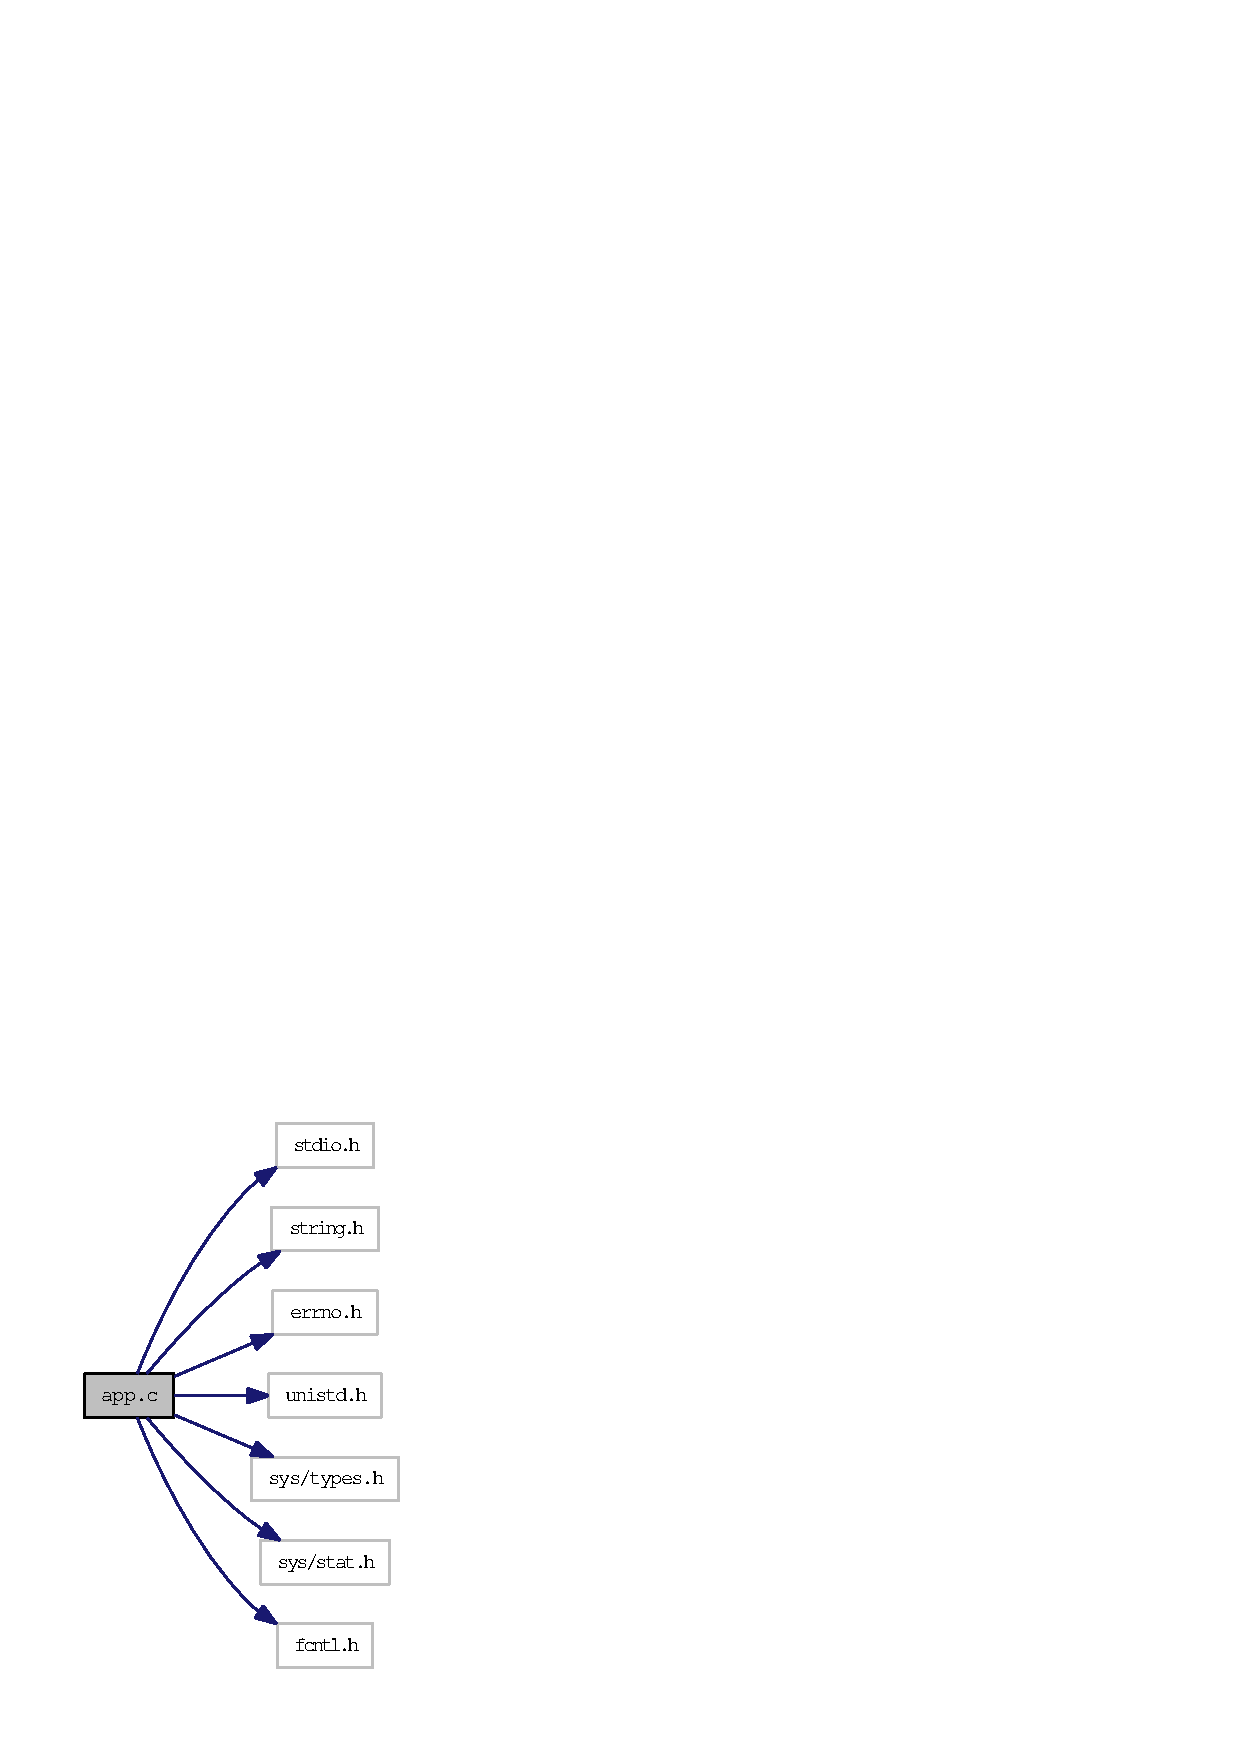
\includegraphics[width=98pt]{app_8c__incl}
\end{center}
\end{figure}
\subsection*{Functions}
\begin{CompactItemize}
\item 
int \hyperlink{app_8c_3c04138a5bfe5d72780bb7e82a18e627}{main} (int argc, char $\ast$$\ast$argv)
\end{CompactItemize}


\subsection{Function Documentation}
\hypertarget{app_8c_3c04138a5bfe5d72780bb7e82a18e627}{
\index{app.c@{app.c}!main@{main}}
\index{main@{main}!app.c@{app.c}}
\subsubsection[main]{\setlength{\rightskip}{0pt plus 5cm}int main (int {\em argc}, char $\ast$$\ast$ {\em argv})}}
\label{app_8c_3c04138a5bfe5d72780bb7e82a18e627}




Definition at line 14 of file app.c.
\hypertarget{bitswapper_8c}{
\section{bitswapper.c File Reference}
\label{bitswapper_8c}\index{bitswapper.c@{bitswapper.c}}
}
{\tt \#include $<$stdio.h$>$}\par
{\tt \#include $<$stdlib.h$>$}\par
{\tt \#include $<$string.h$>$}\par
{\tt \#include $<$unistd.h$>$}\par
{\tt \#include $<$sys/types.h$>$}\par
{\tt \#include $<$linux/types.h$>$}\par
{\tt \#include $<$sys/stat.h$>$}\par
{\tt \#include $<$linux/errno.h$>$}\par
{\tt \#include $<$fcntl.h$>$}\par


Include dependency graph for bitswapper.c:\begin{figure}[H]
\begin{center}
\leavevmode
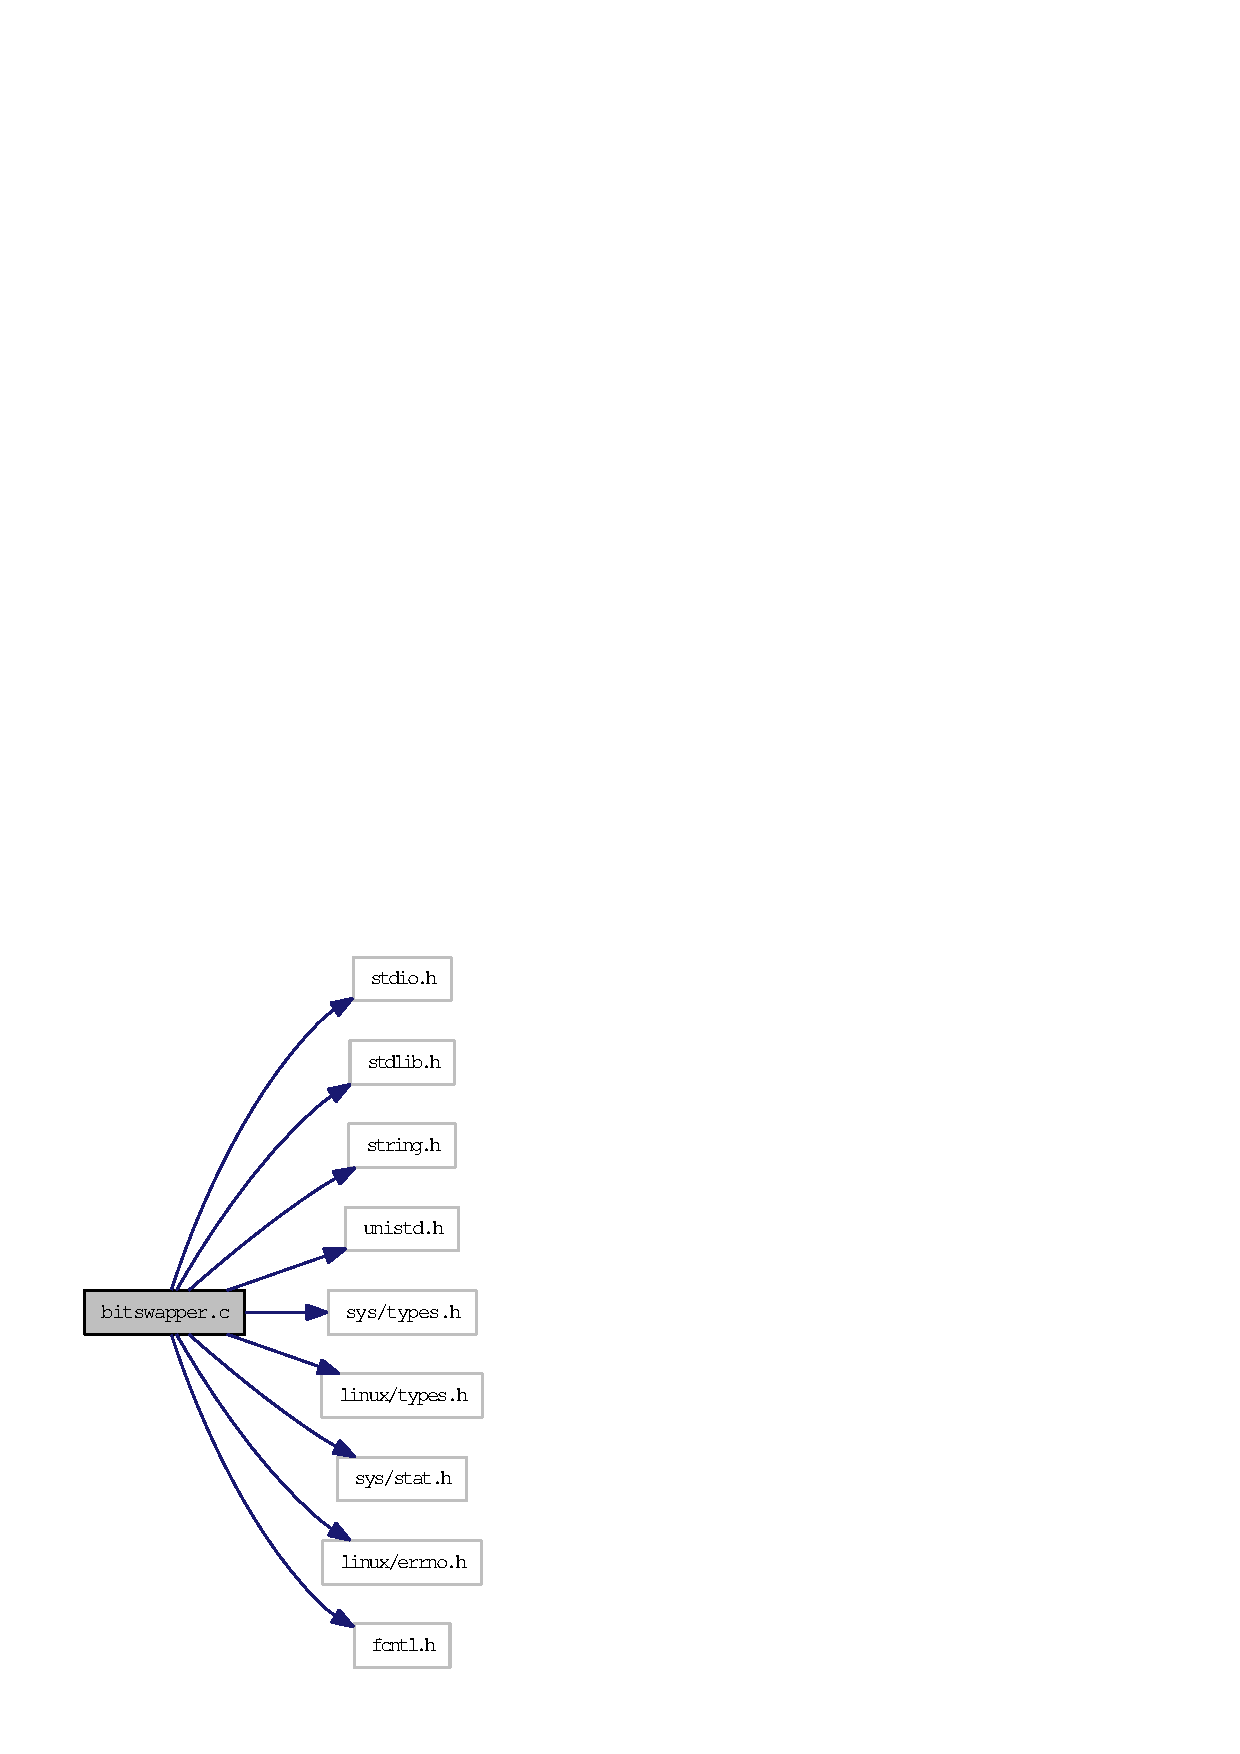
\includegraphics[width=118pt]{bitswapper_8c__incl}
\end{center}
\end{figure}
\subsection*{Functions}
\begin{CompactItemize}
\item 
int \hyperlink{bitswapper_8c_3c04138a5bfe5d72780bb7e82a18e627}{main} (int argc, char $\ast$$\ast$argv)
\item 
int \hyperlink{bitswapper_8c_019759de9c99bad88139a7ca43d05315}{get\-File\-Size} (char $\ast$path)
\begin{CompactList}\small\item\em checks the filesize of a file with the given path \item\end{CompactList}\end{CompactItemize}


\subsection{Function Documentation}
\hypertarget{bitswapper_8c_019759de9c99bad88139a7ca43d05315}{
\index{bitswapper.c@{bitswapper.c}!getFileSize@{getFileSize}}
\index{getFileSize@{getFileSize}!bitswapper.c@{bitswapper.c}}
\subsubsection[getFileSize]{\setlength{\rightskip}{0pt plus 5cm}int get\-File\-Size (char $\ast$ {\em path})}}
\label{bitswapper_8c_019759de9c99bad88139a7ca43d05315}


checks the filesize of a file with the given path 

\begin{Desc}
\item[Returns:]the filesize in Bytes \end{Desc}


Definition at line 88 of file bitswapper.c.

Referenced by do\-Flash\-Frame(), do\-Init(), do\-Scrubbing(), and main().\hypertarget{bitswapper_8c_3c04138a5bfe5d72780bb7e82a18e627}{
\index{bitswapper.c@{bitswapper.c}!main@{main}}
\index{main@{main}!bitswapper.c@{bitswapper.c}}
\subsubsection[main]{\setlength{\rightskip}{0pt plus 5cm}int main (int {\em argc}, char $\ast$$\ast$ {\em argv})}}
\label{bitswapper_8c_3c04138a5bfe5d72780bb7e82a18e627}




Definition at line 29 of file bitswapper.c.

References EXIT\_\-FAILURE, and get\-File\-Size().

Here is the call graph for this function:\begin{figure}[H]
\begin{center}
\leavevmode
\includegraphics[width=93pt]{bitswapper_8c_3c04138a5bfe5d72780bb7e82a18e627_cgraph}
\end{center}
\end{figure}

\hypertarget{bitswapper_8h}{
\section{bitswapper.h File Reference}
\label{bitswapper_8h}\index{bitswapper.h@{bitswapper.h}}
}
The bitswapper to swap files in an 8 bit manner. AA99 5566 -$>$ 99AA 6655. 

\subsection*{Functions}
\begin{CompactItemize}
\item 
int \hyperlink{bitswapper_8h_019759de9c99bad88139a7ca43d05315}{get\-File\-Size} (char $\ast$path)
\end{CompactItemize}


\subsection{Detailed Description}
The bitswapper to swap files in an 8 bit manner. AA99 5566 -$>$ 99AA 6655. 

\begin{Desc}
\item[Author:]Dominik Fehlker \end{Desc}
\begin{Desc}
\item[Date:]\end{Desc}


Definition in file \hyperlink{bitswapper_8h-source}{bitswapper.h}.

\subsection{Function Documentation}
\hypertarget{bitswapper_8h_019759de9c99bad88139a7ca43d05315}{
\index{bitswapper.h@{bitswapper.h}!getFileSize@{getFileSize}}
\index{getFileSize@{getFileSize}!bitswapper.h@{bitswapper.h}}
\subsubsection[getFileSize]{\setlength{\rightskip}{0pt plus 5cm}int get\-File\-Size (char $\ast$ {\em path})}}
\label{bitswapper_8h_019759de9c99bad88139a7ca43d05315}




Definition at line 88 of file bitswapper.c.
\hypertarget{cmdInterpreter_8c}{
\section{cmd\-Interpreter.c File Reference}
\label{cmdInterpreter_8c}\index{cmdInterpreter.c@{cmdInterpreter.c}}
}
{\tt \#include $<$stdio.h$>$}\par
{\tt \#include $<$string.h$>$}\par
{\tt \#include \char`\"{}memoryguard.h\char`\"{}}\par
{\tt \#include $<$errno.h$>$}\par
{\tt \#include $<$sys/types.h$>$}\par
{\tt \#include $<$sys/stat.h$>$}\par
{\tt \#include $<$fcntl.h$>$}\par
{\tt \#include $<$unistd.h$>$}\par
{\tt \#include $<$time.h$>$}\par
{\tt \#include \char`\"{}cmd\-Interpreter.h\char`\"{}}\par
{\tt \#include \char`\"{}dcsc\-Msg\-Buffer\-Interface.h\char`\"{}}\par
{\tt \#include \char`\"{}selectmap\-Interface.h\char`\"{}}\par
{\tt \#include \char`\"{}mrtimers.h\char`\"{}}\par
{\tt \#include \char`\"{}mrshellprim.h\char`\"{}}\par


Include dependency graph for cmd\-Interpreter.c:\begin{figure}[H]
\begin{center}
\leavevmode
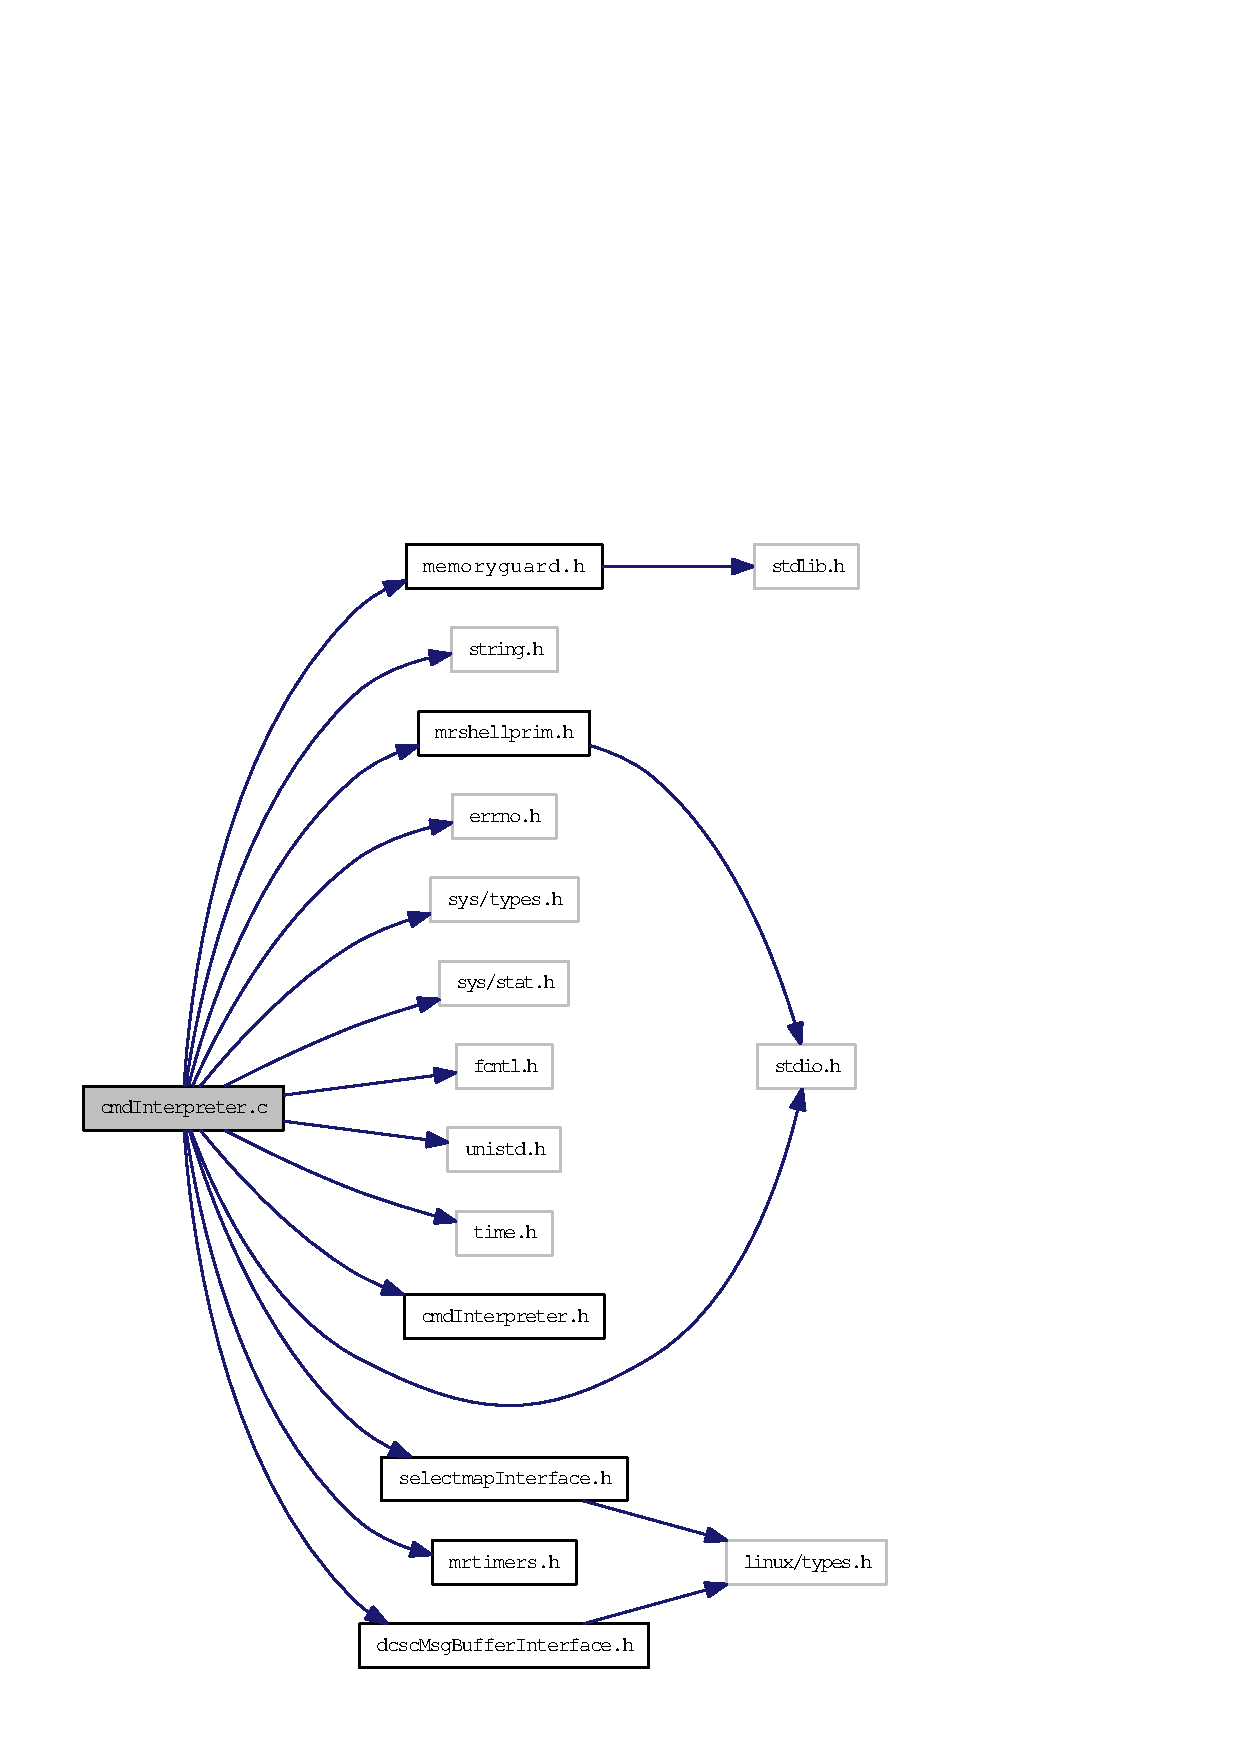
\includegraphics[width=215pt]{cmdInterpreter_8c__incl}
\end{center}
\end{figure}
\subsection*{Data Structures}
\begin{CompactItemize}
\item 
struct \hyperlink{structTCondition}{TCondition}
\end{CompactItemize}
\subsection*{Defines}
\begin{CompactItemize}
\item 
\#define \hyperlink{cmdInterpreter_8c_a2715fedb0c405a7e0062c79494b1ec0}{PRINT\_\-COMMAND\_\-BUFFER\_\-CTR\_\-STRING}~\char`\"{}pcb (print command buffer)\char`\"{}
\item 
\#define \hyperlink{cmdInterpreter_8c_982ee2112f9e2dccdaf82731415a0441}{PRINT\_\-RESULT\_\-BUFFER\_\-CTR\_\-STRING}~\char`\"{}prb (print result buffer)\char`\"{}
\item 
\#define \hyperlink{cmdInterpreter_8c_348a570c30753c168854ec146a2fb53d}{CHECK\_\-COMMAND\_\-BUFFER\_\-CTR\_\-STRING}~\char`\"{}c   (check command buffer)\char`\"{}
\item 
\#define \hyperlink{cmdInterpreter_8c_402f2e4e3254aa689123c78be75bed0a}{IGNORE\_\-BUFFER\_\-CHECK\_\-CTR\_\-STRING}~\char`\"{}i   (ignore buffer check)\char`\"{}
\item 
\#define \hyperlink{cmdInterpreter_8c_997f96a957fef1c6c614fb5cf4b4e3e2}{PRINT\_\-CTRL\_\-REGISTER\_\-CTR\_\-STRING}~\char`\"{}pcr (print control register)\char`\"{}
\item 
\#define \hyperlink{cmdInterpreter_8c_82cf9e89b90c524882e4c7ec0826a37f}{PRINT\_\-COMMAND\_\-RESULT\_\-CTR\_\-STRING}~\char`\"{}r   (print command result)\char`\"{}
\item 
\#define \hyperlink{cmdInterpreter_8c_c880e8e94aca75337b987af06141dcaa}{CMD\_\-STRING\_\-PROFILE}~\char`\"{}profile\char`\"{}
\item 
\#define \hyperlink{cmdInterpreter_8c_5d86dae553f9c8b404487c4f1d3592df}{CMD\_\-STRING\_\-MRT\_\-DEBUG}~\char`\"{}timerdbg\char`\"{}
\end{CompactItemize}
\subsection*{Enumerations}
\begin{CompactItemize}
\item 
enum \hyperlink{cmdInterpreter_8c_ab5835ceff4b64ce6db4148256e0a0f0}{Condition\-Types} \{ \hyperlink{cmdInterpreter_8c_ab5835ceff4b64ce6db4148256e0a0f067fd08219d48244557a06e13926853ee}{e\_\-fail} =  0, 
\hyperlink{cmdInterpreter_8c_ab5835ceff4b64ce6db4148256e0a0f0cb161923a23a717c2d959051d073d65c}{e\_\-continue}
 \}
\end{CompactItemize}
\subsection*{Functions}
\begin{CompactItemize}
\item 
void $\ast$ \hyperlink{cmdInterpreter_8c_46956baca790c8f97d618114d456b1fe}{Convert\-ASCII2Bin} (char $\ast$p\-ASCIIBuffer, int $\ast$pi\-Buffer\-Size, int i\-Word\-Size)
\item 
int \hyperlink{cmdInterpreter_8c_ac3ae2fb745e63e33060d5c0b658f745}{print\-Info} ()
\item 
void \hyperlink{cmdInterpreter_8c_15843554cb32ffb674f4245cfe5ee524}{print\-Debug\-Help} (int i\-Level)
\item 
int \hyperlink{cmdInterpreter_8c_f03f7609a66def2e7fae02a477c38d97}{print\-Help} ()
\item 
void \hyperlink{cmdInterpreter_8c_17ba9ebf0687897855a7c95f19e99c3d}{print\-Read\-Help} ()
\item 
void \hyperlink{cmdInterpreter_8c_c744cdcd05bdccf013ccbc82daa2282a}{print\-Batch\-Proc\-Help} ()
\item 
int \hyperlink{cmdInterpreter_8c_6ead18c93a106e1f1ba5871e908d9916}{read\-Time} (const char $\ast$$\ast$array\-Arg, int i\-Nof\-Args, int $\ast$p\-Sec, int $\ast$p\-Musec)
\item 
int \hyperlink{cmdInterpreter_8c_a78c9a935a342b0b7b9a3c9896c5e85b}{wait\-Condition} (const char $\ast$$\ast$array\-Arg, int i\-Nof\-Args)
\item 
int \hyperlink{cmdInterpreter_8c_f0155066c64e72c64ab000444db4fcad}{build\-Data\-Buffer\-From\-File} (const char $\ast$$\ast$array\-Arg, int nof\-Args, \_\-\_\-u32 $\ast$$\ast$pp\-Buffer, int $\ast$p\-Data\-Format, int i\-Mode)
\item 
int \hyperlink{cmdInterpreter_8c_6f67c6327e24c23440e0fdf83d06e41d}{exec\-Write\-Cmd} (const char $\ast$$\ast$array\-Arg, int i\-Nof\-Args, int i\-Mode)
\begin{CompactList}\small\item\em execute the write command there are 3 argument formats, the argument array is scanned and interpreted according to: 1. \item\end{CompactList}\item 
int \hyperlink{cmdInterpreter_8c_78a2282cf7d3dbf552e5f9876dba01cf}{Scan\-Coefficients} (const char $\ast$p\-Format, float $\ast$pf\-M, float $\ast$pf\-N, \_\-\_\-u32 $\ast$p\-Mask)
\item 
int \hyperlink{cmdInterpreter_8c_e3bcc6695f3c41940a8ab1f428101f07}{print\-Read\-Output\-Formatted} (unsigned char $\ast$\hyperlink{dcscMsgBufferInterface_8c_7fe69f55846ac3a138c130665f1f1e49}{p\-Buffer}, int i\-Buffer\-Size, const char $\ast$p\-Format, int i\-Start\-Address, FILE $\ast$fp)
\item 
int \hyperlink{cmdInterpreter_8c_a7c39db1bcd241c2ae5f259c0281abb6}{exec\-Read\-Cmd} (const char $\ast$$\ast$array\-Arg, int i\-Nof\-Args, int i\-Mode)
\item 
int \hyperlink{cmdInterpreter_8c_ac7fb947e83d5813fb30995133f29955}{timed\-Wait} (int i\-Wait\-Sec, int i\-Wait\-Musec)
\item 
int \hyperlink{cmdInterpreter_8c_ae37490e691f5b4d2c2e8f22713555da}{terminate\-Batch\-Processing} ()
\item 
int \hyperlink{cmdInterpreter_8c_0977826c2ae8c6c45ccfcfa1843cf83c}{exec\-Batch} (const char $\ast$$\ast$array\-Arg, int i\-Nof\-Args)
\item 
int \hyperlink{cmdInterpreter_8c_4a4e70ab937646237dbd0f0db81cdd99}{driver\-Ctrl\-Cmds} (\hyperlink{structArgDef__t}{TArg\-Def} $\ast$p\-Def, void $\ast$p\-User, FILE $\ast$p\-Out)
\item 
int \hyperlink{cmdInterpreter_8c_11ec76f8e60016409f2f33d10c70ef7e}{execute\-Main\-Commands} (const char $\ast$current\-Arg, const char $\ast$$\ast$array\-Arg, int i\-Nof\-Args, void $\ast$p\-User, FILE $\ast$p\-Out)
\item 
int \hyperlink{cmdInterpreter_8c_587fc3f8784e8339c998d9ca71bd7e12}{print\-Flash\-Help} ()
\item 
int \hyperlink{cmdInterpreter_8c_765eadf200d9f408461f7469c791d22c}{exec\-Flash\-Write\-Cmd} (const char $\ast$current\-Arg, const char $\ast$$\ast$array\-Arg, int i\-Nof\-Args, void $\ast$p\-User, FILE $\ast$p\-Out)
\item 
int \hyperlink{cmdInterpreter_8c_5df910c822508a5979806ec5d6548d65}{exec\-Flash\-Verify\-Cmd} (const char $\ast$current\-Arg, const char $\ast$$\ast$array\-Arg, int i\-Nof\-Args, void $\ast$p\-User, FILE $\ast$p\-Out)
\item 
int \hyperlink{cmdInterpreter_8c_0069fb7612546c23d35da357dd126984}{exec\-Flash\-Read\-Cmd} (const char $\ast$current\-Arg, const char $\ast$$\ast$array\-Arg, int i\-Nof\-Args, void $\ast$p\-User, FILE $\ast$p\-Out)
\item 
int \hyperlink{cmdInterpreter_8c_06be82b7d3ea06e8c4d3bc1aca1b63a1}{exec\-Flash\-Eraseall} ()
\item 
int \hyperlink{cmdInterpreter_8c_a4cd43e01e478de0f6dc0cec7ac6152b}{exec\-Flash\-Erase} (\hyperlink{structArgDef__t}{TArg\-Def} $\ast$p\-Def, void $\ast$p\-User, FILE $\ast$p\-Out)
\item 
int \hyperlink{cmdInterpreter_8c_a8f5aca148fba0272ac3acfee150f651}{exec\-Sm\-Write\-Reg} (const char $\ast$current\-Arg, const char $\ast$$\ast$array\-Arg, int i\-Nof\-Args, void $\ast$p\-User, FILE $\ast$p\-Out)
\item 
int \hyperlink{cmdInterpreter_8c_acf8d85528167524bef8a5e23b9ffd99}{exec\-Sm\-Read\-Reg} (const char $\ast$current\-Arg, const char $\ast$$\ast$array\-Arg, int i\-Nof\-Args, void $\ast$p\-User, FILE $\ast$p\-Out)
\item 
int \hyperlink{cmdInterpreter_8c_76b0a4b334ee64eb25b1637d709deb92}{print\-Selectmap\-Help} ()
\item 
int \hyperlink{cmdInterpreter_8c_69279ab735c2dc7e0a73d9c0bfe44f20}{print\-Firmware\-Help} ()
\item 
int \hyperlink{cmdInterpreter_8c_72ffcd5a8ec94bc388af9b6d9781f5de}{exec\-Reg\-Write\-Cmd} (const char $\ast$current\-Arg, const char $\ast$$\ast$array\-Arg, int i\-Nof\-Args, void $\ast$p\-User, FILE $\ast$p\-Out)
\item 
int \hyperlink{cmdInterpreter_8c_371d348f7b5d98c0ad4e7d6d20deb65c}{exec\-Reg\-Read\-Cmd} (const char $\ast$current\-Arg, const char $\ast$$\ast$array\-Arg, int i\-Nof\-Args, void $\ast$p\-User, FILE $\ast$p\-Out)
\item 
int \hyperlink{cmdInterpreter_8c_7c4a53b4c0e418e7102cba28b663fbb5}{ctrl\-Reg\-Status} ()
\item 
int \hyperlink{cmdInterpreter_8c_54cbd6e4f4a91310f0c408dc5c6b413d}{execute\-Command\-Args} (int i\-Nof\-Args, const char $\ast$$\ast$array\-Arg)
\item 
int \hyperlink{cmdInterpreter_8c_48086998882e7d163126de4100aa12ac}{execute\-Command\-Line} (char $\ast$p\-Cmd\-Line)
\end{CompactItemize}
\subsection*{Variables}
\begin{CompactItemize}
\item 
int \hyperlink{cmdInterpreter_8c_b1b44b602185677d4a2a372121627437}{g\_\-profiling} = 0
\item 
int \hyperlink{cmdInterpreter_8c_0aee2ec97f7e88992f9b2b333ca99be2}{g\_\-b\-Batch\-Processing} = 0
\item 
\hyperlink{structArgDef__t}{TArg\-Def} \hyperlink{cmdInterpreter_8c_083a182722ef62f10a68012ab6d7f707}{driver\-Ctrl\-Args} \mbox{[}$\,$\mbox{]}
\item 
\hyperlink{structFctArg__t}{TFct\-Arg} \hyperlink{cmdInterpreter_8c_3e75245c450c10d2323442d359f053d7}{driver\-Ctrl\-Desc}
\item 
\hyperlink{structFctMode__t}{TFct\-Mode} \hyperlink{cmdInterpreter_8c_fbc09bb85c6e4618a38dba855c588abd}{scan\-Mode\-Default} = \{SCANMODE\_\-FORCE\_\-TERMINATION, NULL, NULL\}
\item 
\hyperlink{structArgDef__t}{TArg\-Def} \hyperlink{cmdInterpreter_8c_4954a4ac4d6f82836d8b405a2ec86071}{selectmap\-Cmds} \mbox{[}$\,$\mbox{]}
\item 
\hyperlink{structArgDef__t}{TArg\-Def} \hyperlink{cmdInterpreter_8c_7399e2dab99f698c9275622762e94f74}{flash\-Erase\-Params} \mbox{[}$\,$\mbox{]}
\item 
\hyperlink{structFctArg__t}{TFct\-Arg} \hyperlink{cmdInterpreter_8c_9a757fd68a4d59000e0938fcdb423996}{flash\-Erase\-Desc}
\item 
\hyperlink{structArgDef__t}{TArg\-Def} \hyperlink{cmdInterpreter_8c_5a3ddbaacf0c338e408e3c0b55189d58}{flash\-Cmds} \mbox{[}$\,$\mbox{]}
\item 
\hyperlink{structArgDef__t}{TArg\-Def} \hyperlink{cmdInterpreter_8c_5a94aee581a390576806909f67968c30}{firmware\-Cmds} \mbox{[}$\,$\mbox{]}
\item 
\hyperlink{structArgDef__t}{TArg\-Def} \hyperlink{cmdInterpreter_8c_c1784239c15c2f1b5b4f1dbda9df65e7}{ctrl\-Reg\-Cmds} \mbox{[}$\,$\mbox{]}
\item 
\hyperlink{structArgDef__t}{TArg\-Def} \hyperlink{cmdInterpreter_8c_014d78494c13d4dc0430ee68de158559}{main\-Commands} \mbox{[}$\,$\mbox{]}
\end{CompactItemize}


\subsection{Define Documentation}
\hypertarget{cmdInterpreter_8c_348a570c30753c168854ec146a2fb53d}{
\index{cmdInterpreter.c@{cmd\-Interpreter.c}!CHECK_COMMAND_BUFFER_CTR_STRING@{CHECK\_\-COMMAND\_\-BUFFER\_\-CTR\_\-STRING}}
\index{CHECK_COMMAND_BUFFER_CTR_STRING@{CHECK\_\-COMMAND\_\-BUFFER\_\-CTR\_\-STRING}!cmdInterpreter.c@{cmd\-Interpreter.c}}
\subsubsection[CHECK\_\-COMMAND\_\-BUFFER\_\-CTR\_\-STRING]{\setlength{\rightskip}{0pt plus 5cm}\#define CHECK\_\-COMMAND\_\-BUFFER\_\-CTR\_\-STRING~\char`\"{}c   (check command buffer)\char`\"{}}}
\label{cmdInterpreter_8c_348a570c30753c168854ec146a2fb53d}




Definition at line 41 of file cmd\-Interpreter.c.\hypertarget{cmdInterpreter_8c_5d86dae553f9c8b404487c4f1d3592df}{
\index{cmdInterpreter.c@{cmd\-Interpreter.c}!CMD_STRING_MRT_DEBUG@{CMD\_\-STRING\_\-MRT\_\-DEBUG}}
\index{CMD_STRING_MRT_DEBUG@{CMD\_\-STRING\_\-MRT\_\-DEBUG}!cmdInterpreter.c@{cmd\-Interpreter.c}}
\subsubsection[CMD\_\-STRING\_\-MRT\_\-DEBUG]{\setlength{\rightskip}{0pt plus 5cm}\#define CMD\_\-STRING\_\-MRT\_\-DEBUG~\char`\"{}timerdbg\char`\"{}}}
\label{cmdInterpreter_8c_5d86dae553f9c8b404487c4f1d3592df}




Definition at line 46 of file cmd\-Interpreter.c.

Referenced by execute\-Main\-Commands().\hypertarget{cmdInterpreter_8c_c880e8e94aca75337b987af06141dcaa}{
\index{cmdInterpreter.c@{cmd\-Interpreter.c}!CMD_STRING_PROFILE@{CMD\_\-STRING\_\-PROFILE}}
\index{CMD_STRING_PROFILE@{CMD\_\-STRING\_\-PROFILE}!cmdInterpreter.c@{cmd\-Interpreter.c}}
\subsubsection[CMD\_\-STRING\_\-PROFILE]{\setlength{\rightskip}{0pt plus 5cm}\#define CMD\_\-STRING\_\-PROFILE~\char`\"{}profile\char`\"{}}}
\label{cmdInterpreter_8c_c880e8e94aca75337b987af06141dcaa}




Definition at line 45 of file cmd\-Interpreter.c.

Referenced by execute\-Main\-Commands().\hypertarget{cmdInterpreter_8c_402f2e4e3254aa689123c78be75bed0a}{
\index{cmdInterpreter.c@{cmd\-Interpreter.c}!IGNORE_BUFFER_CHECK_CTR_STRING@{IGNORE\_\-BUFFER\_\-CHECK\_\-CTR\_\-STRING}}
\index{IGNORE_BUFFER_CHECK_CTR_STRING@{IGNORE\_\-BUFFER\_\-CHECK\_\-CTR\_\-STRING}!cmdInterpreter.c@{cmd\-Interpreter.c}}
\subsubsection[IGNORE\_\-BUFFER\_\-CHECK\_\-CTR\_\-STRING]{\setlength{\rightskip}{0pt plus 5cm}\#define IGNORE\_\-BUFFER\_\-CHECK\_\-CTR\_\-STRING~\char`\"{}i   (ignore buffer check)\char`\"{}}}
\label{cmdInterpreter_8c_402f2e4e3254aa689123c78be75bed0a}




Definition at line 42 of file cmd\-Interpreter.c.\hypertarget{cmdInterpreter_8c_a2715fedb0c405a7e0062c79494b1ec0}{
\index{cmdInterpreter.c@{cmd\-Interpreter.c}!PRINT_COMMAND_BUFFER_CTR_STRING@{PRINT\_\-COMMAND\_\-BUFFER\_\-CTR\_\-STRING}}
\index{PRINT_COMMAND_BUFFER_CTR_STRING@{PRINT\_\-COMMAND\_\-BUFFER\_\-CTR\_\-STRING}!cmdInterpreter.c@{cmd\-Interpreter.c}}
\subsubsection[PRINT\_\-COMMAND\_\-BUFFER\_\-CTR\_\-STRING]{\setlength{\rightskip}{0pt plus 5cm}\#define PRINT\_\-COMMAND\_\-BUFFER\_\-CTR\_\-STRING~\char`\"{}pcb (print command buffer)\char`\"{}}}
\label{cmdInterpreter_8c_a2715fedb0c405a7e0062c79494b1ec0}




Definition at line 39 of file cmd\-Interpreter.c.\hypertarget{cmdInterpreter_8c_82cf9e89b90c524882e4c7ec0826a37f}{
\index{cmdInterpreter.c@{cmd\-Interpreter.c}!PRINT_COMMAND_RESULT_CTR_STRING@{PRINT\_\-COMMAND\_\-RESULT\_\-CTR\_\-STRING}}
\index{PRINT_COMMAND_RESULT_CTR_STRING@{PRINT\_\-COMMAND\_\-RESULT\_\-CTR\_\-STRING}!cmdInterpreter.c@{cmd\-Interpreter.c}}
\subsubsection[PRINT\_\-COMMAND\_\-RESULT\_\-CTR\_\-STRING]{\setlength{\rightskip}{0pt plus 5cm}\#define PRINT\_\-COMMAND\_\-RESULT\_\-CTR\_\-STRING~\char`\"{}r   (print command result)\char`\"{}}}
\label{cmdInterpreter_8c_82cf9e89b90c524882e4c7ec0826a37f}




Definition at line 44 of file cmd\-Interpreter.c.\hypertarget{cmdInterpreter_8c_997f96a957fef1c6c614fb5cf4b4e3e2}{
\index{cmdInterpreter.c@{cmd\-Interpreter.c}!PRINT_CTRL_REGISTER_CTR_STRING@{PRINT\_\-CTRL\_\-REGISTER\_\-CTR\_\-STRING}}
\index{PRINT_CTRL_REGISTER_CTR_STRING@{PRINT\_\-CTRL\_\-REGISTER\_\-CTR\_\-STRING}!cmdInterpreter.c@{cmd\-Interpreter.c}}
\subsubsection[PRINT\_\-CTRL\_\-REGISTER\_\-CTR\_\-STRING]{\setlength{\rightskip}{0pt plus 5cm}\#define PRINT\_\-CTRL\_\-REGISTER\_\-CTR\_\-STRING~\char`\"{}pcr (print control register)\char`\"{}}}
\label{cmdInterpreter_8c_997f96a957fef1c6c614fb5cf4b4e3e2}




Definition at line 43 of file cmd\-Interpreter.c.\hypertarget{cmdInterpreter_8c_982ee2112f9e2dccdaf82731415a0441}{
\index{cmdInterpreter.c@{cmd\-Interpreter.c}!PRINT_RESULT_BUFFER_CTR_STRING@{PRINT\_\-RESULT\_\-BUFFER\_\-CTR\_\-STRING}}
\index{PRINT_RESULT_BUFFER_CTR_STRING@{PRINT\_\-RESULT\_\-BUFFER\_\-CTR\_\-STRING}!cmdInterpreter.c@{cmd\-Interpreter.c}}
\subsubsection[PRINT\_\-RESULT\_\-BUFFER\_\-CTR\_\-STRING]{\setlength{\rightskip}{0pt plus 5cm}\#define PRINT\_\-RESULT\_\-BUFFER\_\-CTR\_\-STRING~\char`\"{}prb (print result buffer)\char`\"{}}}
\label{cmdInterpreter_8c_982ee2112f9e2dccdaf82731415a0441}




Definition at line 40 of file cmd\-Interpreter.c.

\subsection{Enumeration Type Documentation}
\hypertarget{cmdInterpreter_8c_ab5835ceff4b64ce6db4148256e0a0f0}{
\index{cmdInterpreter.c@{cmd\-Interpreter.c}!ConditionTypes@{ConditionTypes}}
\index{ConditionTypes@{ConditionTypes}!cmdInterpreter.c@{cmd\-Interpreter.c}}
\subsubsection[ConditionTypes]{\setlength{\rightskip}{0pt plus 5cm}enum \hyperlink{cmdInterpreter_8c_ab5835ceff4b64ce6db4148256e0a0f0}{Condition\-Types}}}
\label{cmdInterpreter_8c_ab5835ceff4b64ce6db4148256e0a0f0}


\begin{Desc}
\item[Enumerator: ]\par
\begin{description}
\index{e_fail@{e\_\-fail}!cmdInterpreter.c@{cmdInterpreter.c}}\index{cmdInterpreter.c@{cmdInterpreter.c}!e_fail@{e\_\-fail}}\item[{\em 
\hypertarget{cmdInterpreter_8c_ab5835ceff4b64ce6db4148256e0a0f067fd08219d48244557a06e13926853ee}{
e\_\-fail}
\label{cmdInterpreter_8c_ab5835ceff4b64ce6db4148256e0a0f067fd08219d48244557a06e13926853ee}
}]\index{e_continue@{e\_\-continue}!cmdInterpreter.c@{cmdInterpreter.c}}\index{cmdInterpreter.c@{cmdInterpreter.c}!e_continue@{e\_\-continue}}\item[{\em 
\hypertarget{cmdInterpreter_8c_ab5835ceff4b64ce6db4148256e0a0f0cb161923a23a717c2d959051d073d65c}{
e\_\-continue}
\label{cmdInterpreter_8c_ab5835ceff4b64ce6db4148256e0a0f0cb161923a23a717c2d959051d073d65c}
}]\end{description}
\end{Desc}



Definition at line 73 of file cmd\-Interpreter.c.

\subsection{Function Documentation}
\hypertarget{cmdInterpreter_8c_f0155066c64e72c64ab000444db4fcad}{
\index{cmdInterpreter.c@{cmd\-Interpreter.c}!buildDataBufferFromFile@{buildDataBufferFromFile}}
\index{buildDataBufferFromFile@{buildDataBufferFromFile}!cmdInterpreter.c@{cmd\-Interpreter.c}}
\subsubsection[buildDataBufferFromFile]{\setlength{\rightskip}{0pt plus 5cm}int build\-Data\-Buffer\-From\-File (const char $\ast$$\ast$ {\em array\-Arg}, int {\em nof\-Args}, \_\-\_\-u32 $\ast$$\ast$ {\em pp\-Buffer}, int $\ast$ {\em p\-Data\-Format}, int {\em i\-Mode})}}
\label{cmdInterpreter_8c_f0155066c64e72c64ab000444db4fcad}




Definition at line 490 of file cmd\-Interpreter.c.

References Convert\-ASCII2Bin(), DBG\_\-FILE\_\-CONVERT, get\-Dec\-Number\-From\-Arg(), and set\-Debug\-Option\-Flag().

Referenced by exec\-Write\-Cmd().

Here is the call graph for this function:\begin{figure}[H]
\begin{center}
\leavevmode
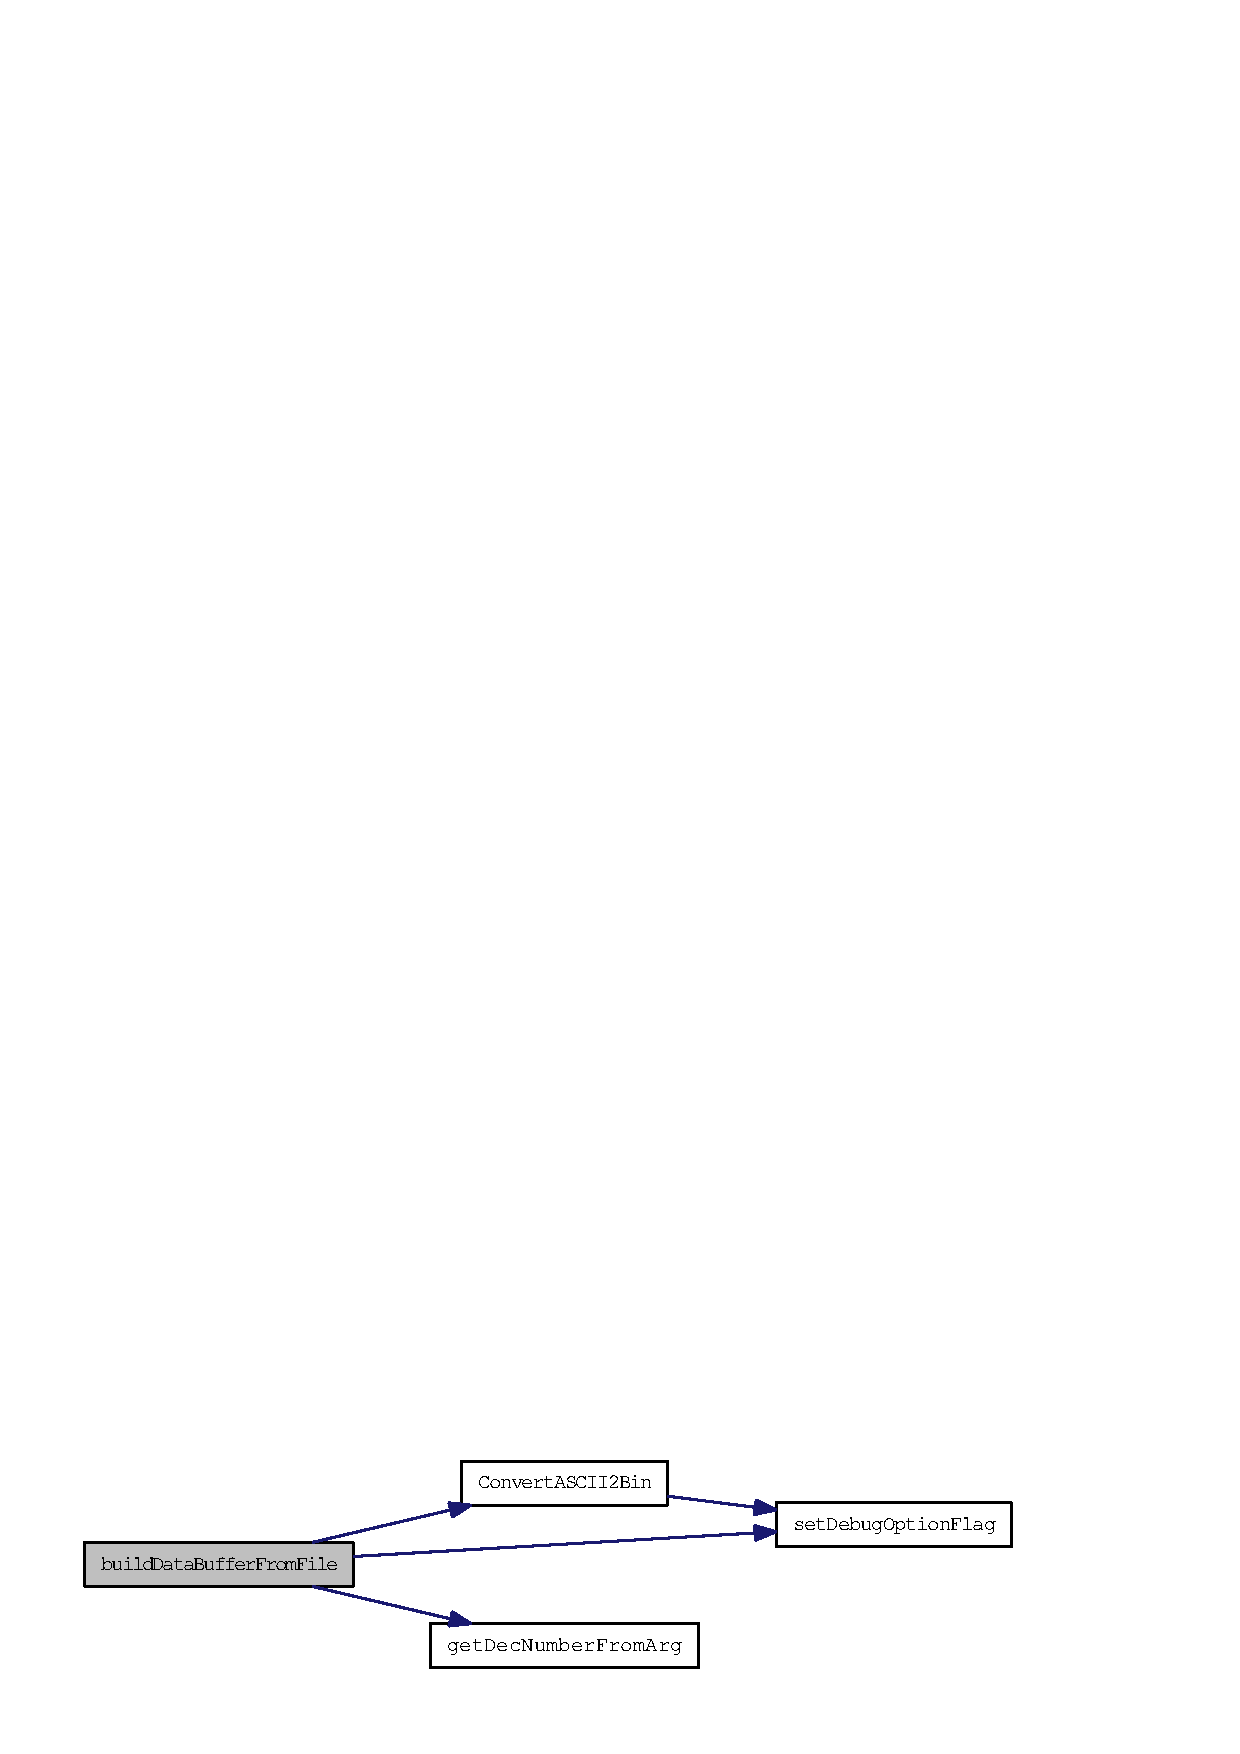
\includegraphics[width=245pt]{cmdInterpreter_8c_f0155066c64e72c64ab000444db4fcad_cgraph}
\end{center}
\end{figure}
\hypertarget{cmdInterpreter_8c_46956baca790c8f97d618114d456b1fe}{
\index{cmdInterpreter.c@{cmd\-Interpreter.c}!ConvertASCII2Bin@{ConvertASCII2Bin}}
\index{ConvertASCII2Bin@{ConvertASCII2Bin}!cmdInterpreter.c@{cmd\-Interpreter.c}}
\subsubsection[ConvertASCII2Bin]{\setlength{\rightskip}{0pt plus 5cm}void$\ast$ Convert\-ASCII2Bin (char $\ast$ {\em p\-ASCIIBuffer}, int $\ast$ {\em pi\-Buffer\-Size}, int {\em i\-Word\-Size})}}
\label{cmdInterpreter_8c_46956baca790c8f97d618114d456b1fe}




Definition at line 84 of file cmd\-Interpreter.c.

References DBG\_\-FILE\_\-CONVERT, and set\-Debug\-Option\-Flag().

Referenced by build\-Data\-Buffer\-From\-File().

Here is the call graph for this function:\begin{figure}[H]
\begin{center}
\leavevmode
\includegraphics[width=147pt]{cmdInterpreter_8c_46956baca790c8f97d618114d456b1fe_cgraph}
\end{center}
\end{figure}
\hypertarget{cmdInterpreter_8c_7c4a53b4c0e418e7102cba28b663fbb5}{
\index{cmdInterpreter.c@{cmd\-Interpreter.c}!ctrlRegStatus@{ctrlRegStatus}}
\index{ctrlRegStatus@{ctrlRegStatus}!cmdInterpreter.c@{cmd\-Interpreter.c}}
\subsubsection[ctrlRegStatus]{\setlength{\rightskip}{0pt plus 5cm}int ctrl\-Reg\-Status ()}}
\label{cmdInterpreter_8c_7c4a53b4c0e418e7102cba28b663fbb5}




Definition at line 1816 of file cmd\-Interpreter.c.

References e\-Read\-Ctrl\-Reg, and rcu\-Bus\-Control\-Cmd().

Here is the call graph for this function:\begin{figure}[H]
\begin{center}
\leavevmode
\includegraphics[width=212pt]{cmdInterpreter_8c_7c4a53b4c0e418e7102cba28b663fbb5_cgraph}
\end{center}
\end{figure}
\hypertarget{cmdInterpreter_8c_4a4e70ab937646237dbd0f0db81cdd99}{
\index{cmdInterpreter.c@{cmd\-Interpreter.c}!driverCtrlCmds@{driverCtrlCmds}}
\index{driverCtrlCmds@{driverCtrlCmds}!cmdInterpreter.c@{cmd\-Interpreter.c}}
\subsubsection[driverCtrlCmds]{\setlength{\rightskip}{0pt plus 5cm}int driver\-Ctrl\-Cmds (\hyperlink{structArgDef__t}{TArg\-Def} $\ast$ {\em p\-Def}, void $\ast$ {\em p\-User}, FILE $\ast$ {\em p\-Out})}}
\label{cmdInterpreter_8c_4a4e70ab937646237dbd0f0db81cdd99}




Definition at line 1445 of file cmd\-Interpreter.c.

References ARGPROC\_\-EXISTS, dcsc\-Driver\-Debug(), and mr\-Shell\-Prim\-Get\-Hex().

Here is the call graph for this function:\begin{figure}[H]
\begin{center}
\leavevmode
\includegraphics[width=215pt]{cmdInterpreter_8c_4a4e70ab937646237dbd0f0db81cdd99_cgraph}
\end{center}
\end{figure}
\hypertarget{cmdInterpreter_8c_0977826c2ae8c6c45ccfcfa1843cf83c}{
\index{cmdInterpreter.c@{cmd\-Interpreter.c}!execBatch@{execBatch}}
\index{execBatch@{execBatch}!cmdInterpreter.c@{cmd\-Interpreter.c}}
\subsubsection[execBatch]{\setlength{\rightskip}{0pt plus 5cm}int exec\-Batch (const char $\ast$$\ast$ {\em array\-Arg}, int {\em i\-Nof\-Args})}}
\label{cmdInterpreter_8c_0977826c2ae8c6c45ccfcfa1843cf83c}




Definition at line 1294 of file cmd\-Interpreter.c.

References execute\-Command\-Line(), g\_\-b\-Batch\-Processing, g\_\-profiling, get\-Dec\-Number\-From\-Arg(), get\-Timer\-Value\-String(), read\-Time(), remove\-Prec\-And\-Trailing\-Spec\-Chars(), start\-Timer(), stop\-Timer(), and timed\-Wait().

Referenced by execute\-Main\-Commands().

Here is the call graph for this function:\begin{figure}[H]
\begin{center}
\leavevmode
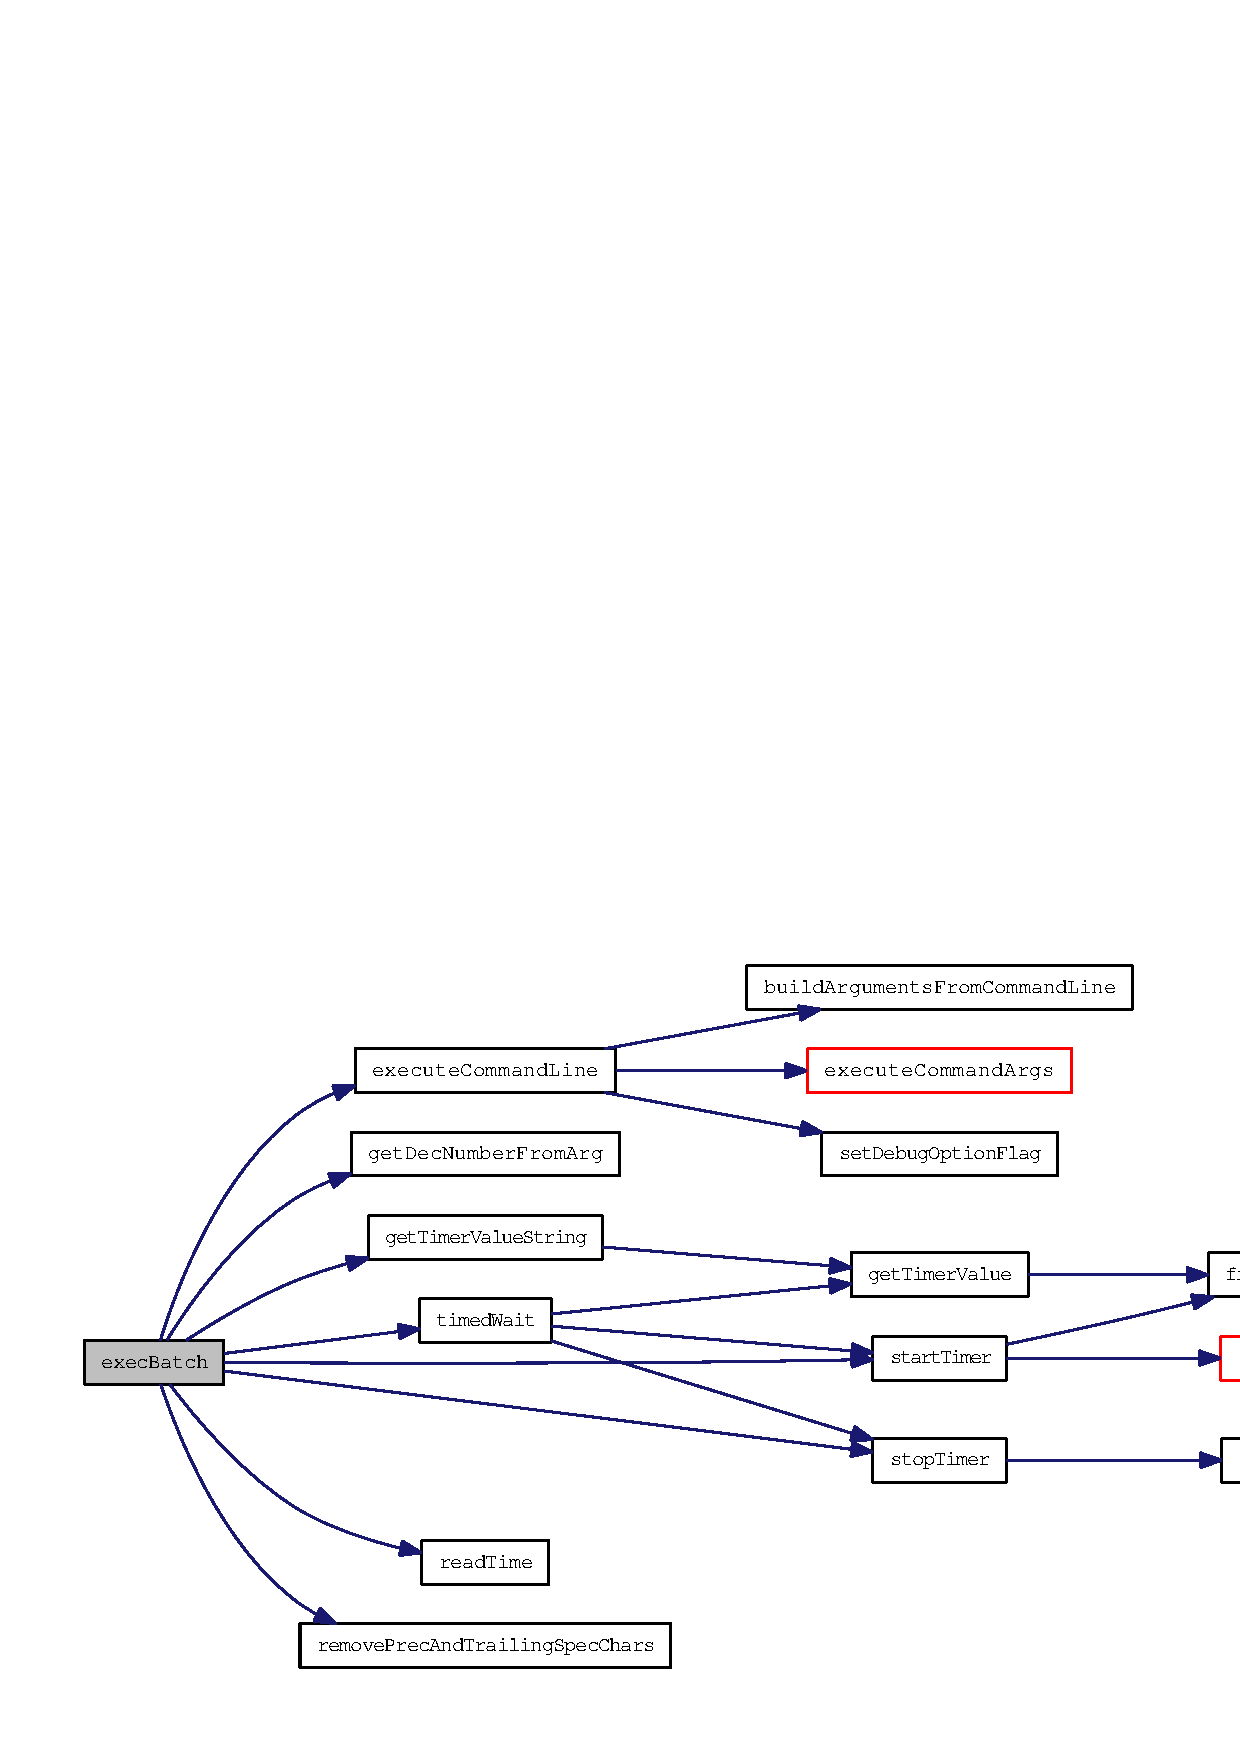
\includegraphics[width=335pt]{cmdInterpreter_8c_0977826c2ae8c6c45ccfcfa1843cf83c_cgraph}
\end{center}
\end{figure}
\hypertarget{cmdInterpreter_8c_a4cd43e01e478de0f6dc0cec7ac6152b}{
\index{cmdInterpreter.c@{cmd\-Interpreter.c}!execFlashErase@{execFlashErase}}
\index{execFlashErase@{execFlashErase}!cmdInterpreter.c@{cmd\-Interpreter.c}}
\subsubsection[execFlashErase]{\setlength{\rightskip}{0pt plus 5cm}int exec\-Flash\-Erase (\hyperlink{structArgDef__t}{TArg\-Def} $\ast$ {\em p\-Def}, void $\ast$ {\em p\-User}, FILE $\ast$ {\em p\-Out})}}
\label{cmdInterpreter_8c_a4cd43e01e478de0f6dc0cec7ac6152b}




Definition at line 1723 of file cmd\-Interpreter.c.

References ARGPROC\_\-EXISTS, mr\-Shell\-Prim\-Get\-Hex(), mr\-Shell\-Prim\-Get\-Int(), and rcu\-Flash\-Erase().

Here is the call graph for this function:\begin{figure}[H]
\begin{center}
\leavevmode
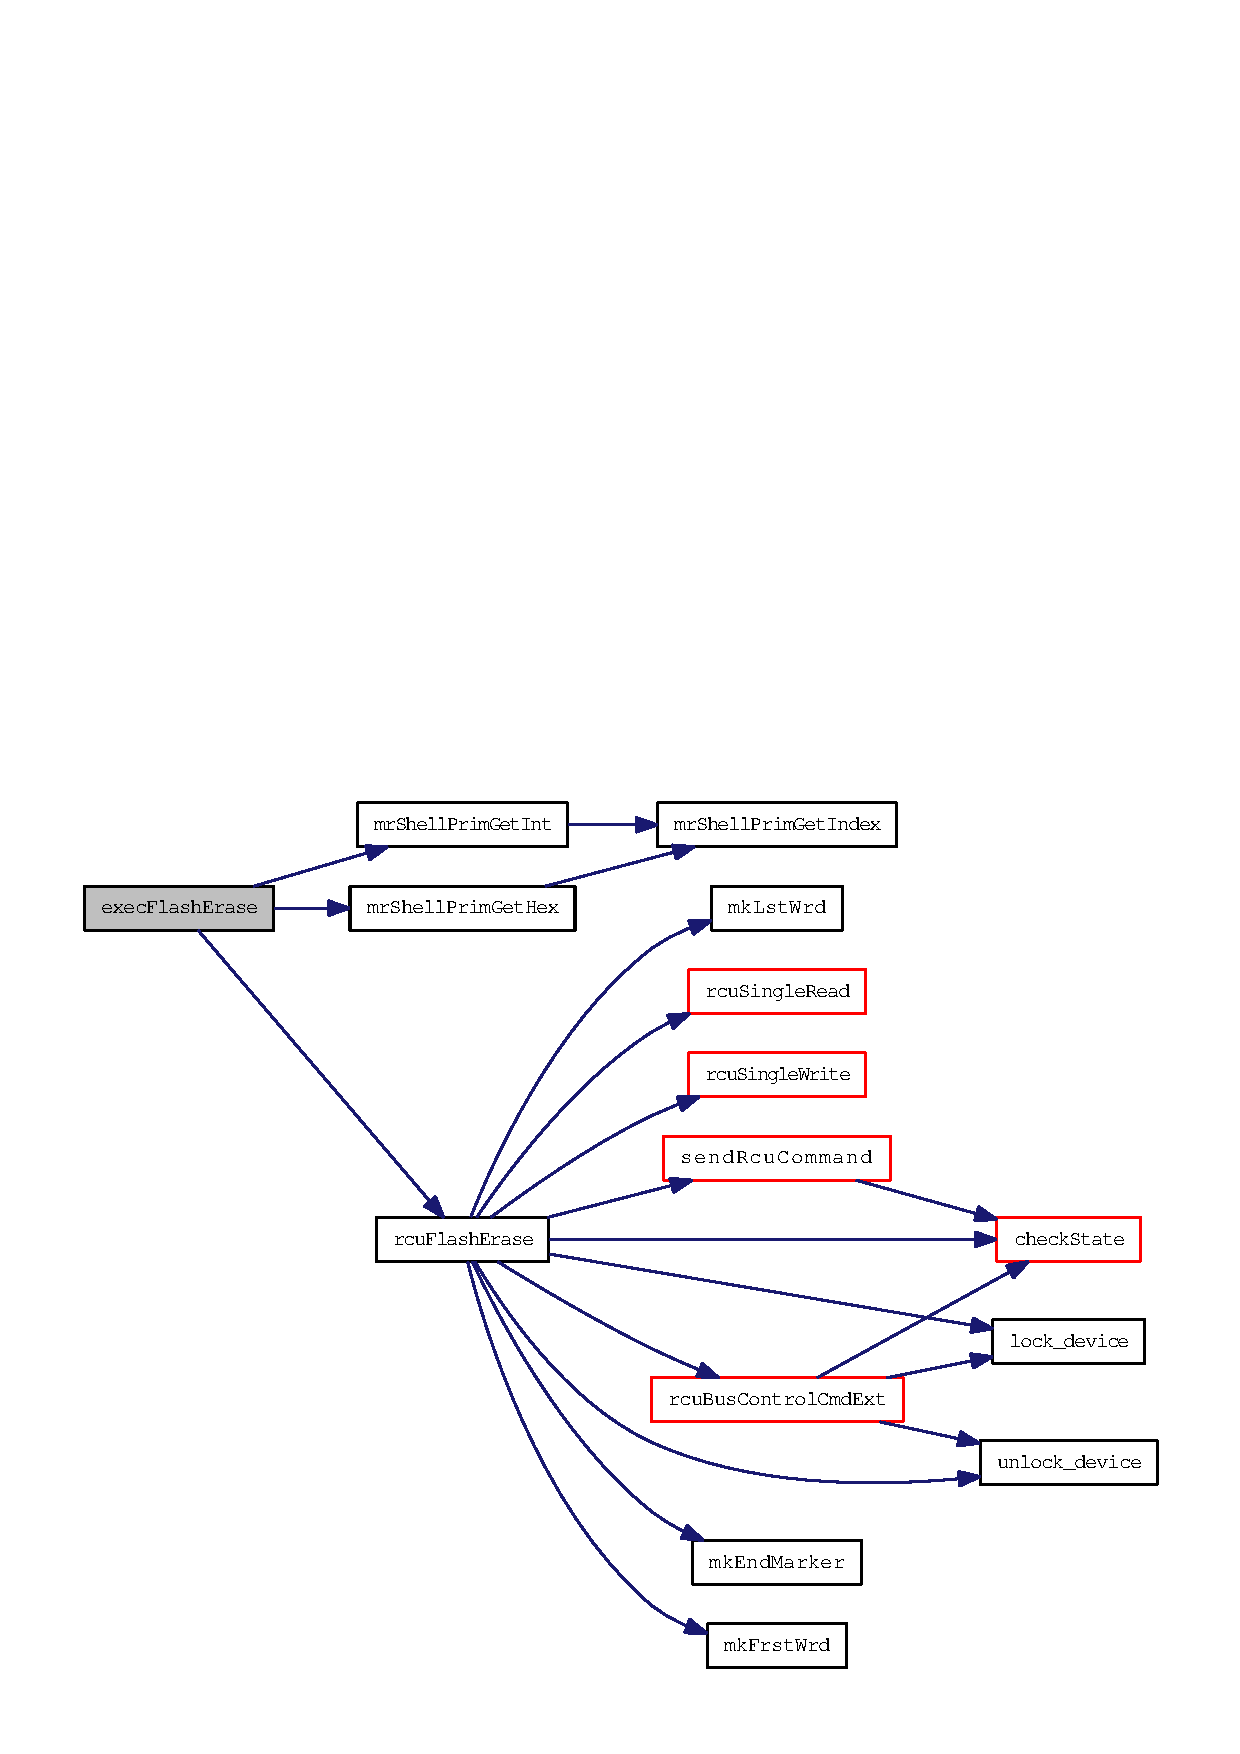
\includegraphics[width=280pt]{cmdInterpreter_8c_a4cd43e01e478de0f6dc0cec7ac6152b_cgraph}
\end{center}
\end{figure}
\hypertarget{cmdInterpreter_8c_06be82b7d3ea06e8c4d3bc1aca1b63a1}{
\index{cmdInterpreter.c@{cmd\-Interpreter.c}!execFlashEraseall@{execFlashEraseall}}
\index{execFlashEraseall@{execFlashEraseall}!cmdInterpreter.c@{cmd\-Interpreter.c}}
\subsubsection[execFlashEraseall]{\setlength{\rightskip}{0pt plus 5cm}int exec\-Flash\-Eraseall ()}}
\label{cmdInterpreter_8c_06be82b7d3ea06e8c4d3bc1aca1b63a1}




Definition at line 1718 of file cmd\-Interpreter.c.

References rcu\-Flash\-Erase().

Here is the call graph for this function:\begin{figure}[H]
\begin{center}
\leavevmode
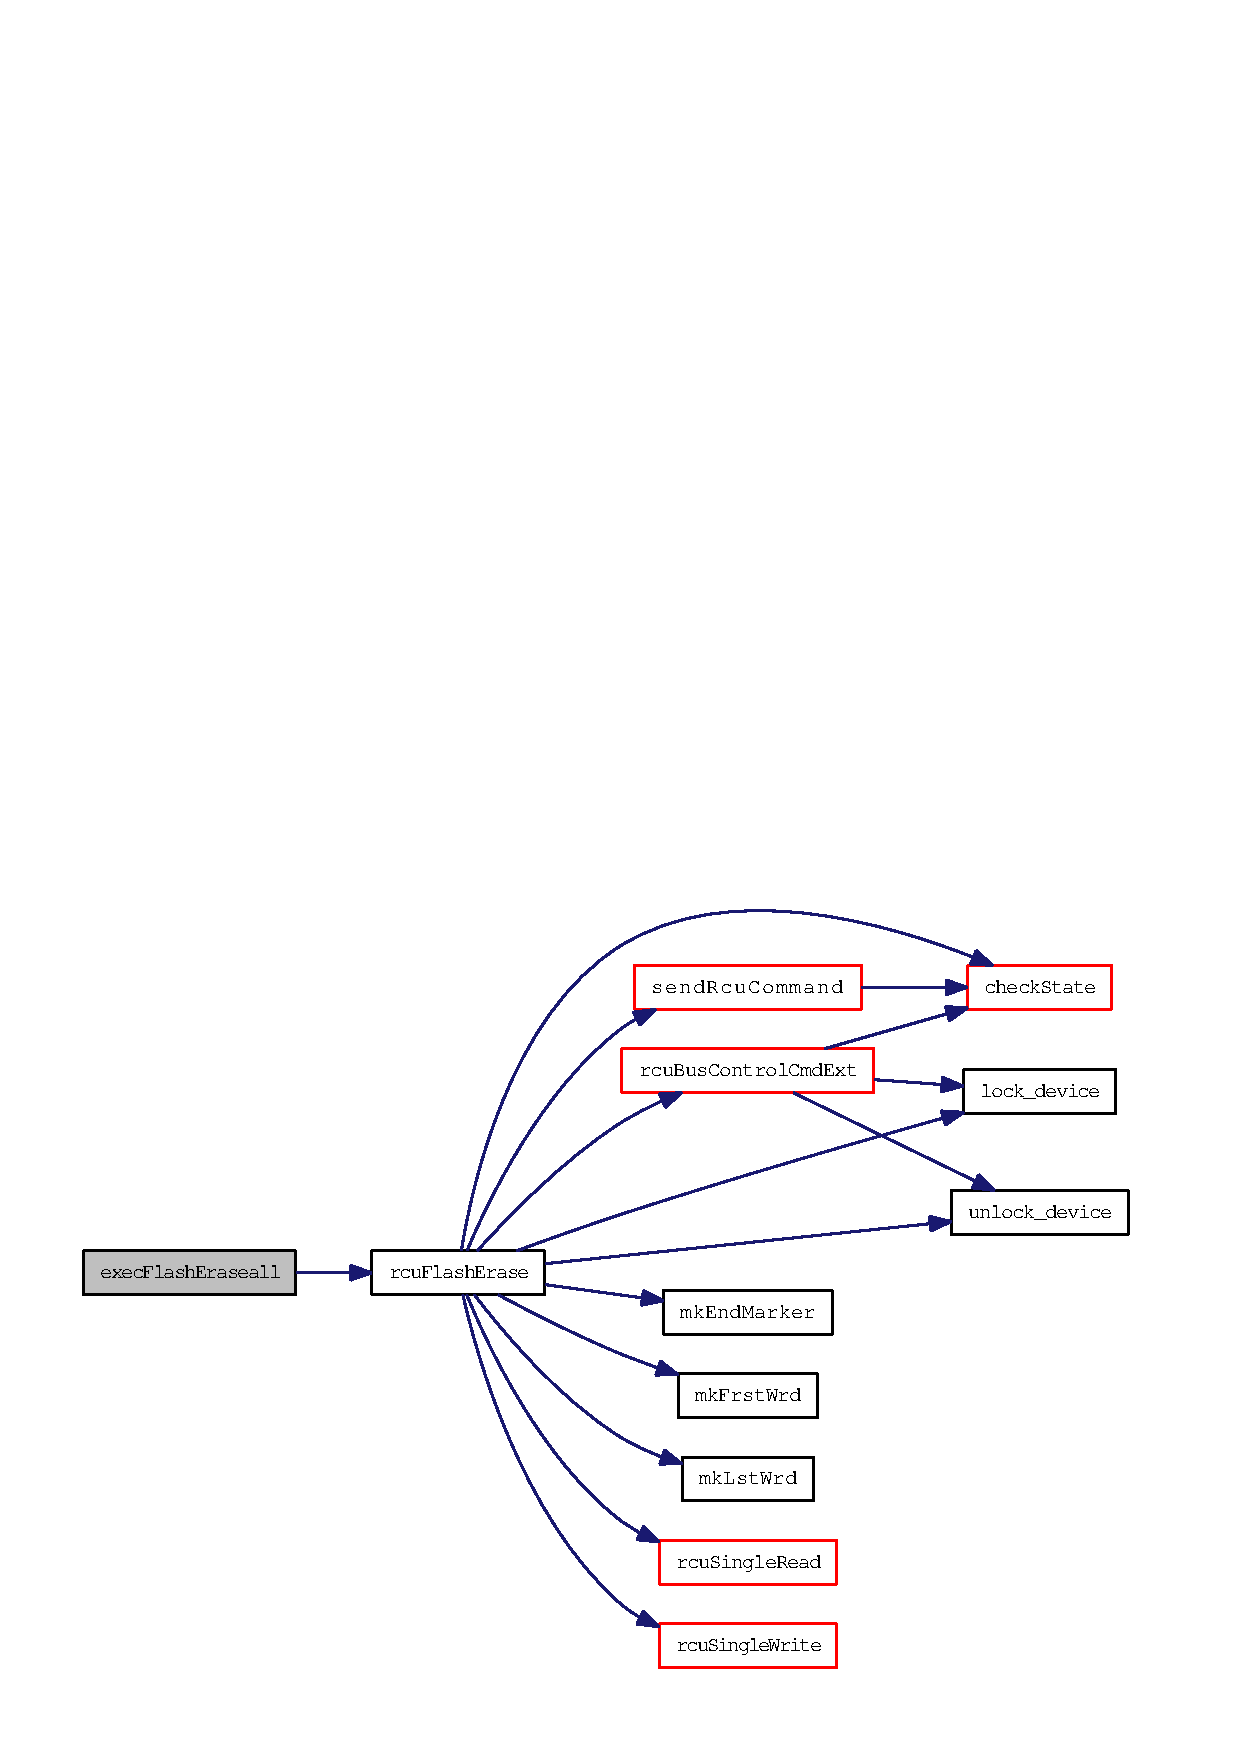
\includegraphics[width=273pt]{cmdInterpreter_8c_06be82b7d3ea06e8c4d3bc1aca1b63a1_cgraph}
\end{center}
\end{figure}
\hypertarget{cmdInterpreter_8c_0069fb7612546c23d35da357dd126984}{
\index{cmdInterpreter.c@{cmd\-Interpreter.c}!execFlashReadCmd@{execFlashReadCmd}}
\index{execFlashReadCmd@{execFlashReadCmd}!cmdInterpreter.c@{cmd\-Interpreter.c}}
\subsubsection[execFlashReadCmd]{\setlength{\rightskip}{0pt plus 5cm}int exec\-Flash\-Read\-Cmd (const char $\ast$ {\em current\-Arg}, const char $\ast$$\ast$ {\em array\-Arg}, int {\em i\-Nof\-Args}, void $\ast$ {\em p\-User}, FILE $\ast$ {\em p\-Out})}}
\label{cmdInterpreter_8c_0069fb7612546c23d35da357dd126984}




Definition at line 1711 of file cmd\-Interpreter.c.

References exec\-Read\-Cmd().

Here is the call graph for this function:\begin{figure}[H]
\begin{center}
\leavevmode
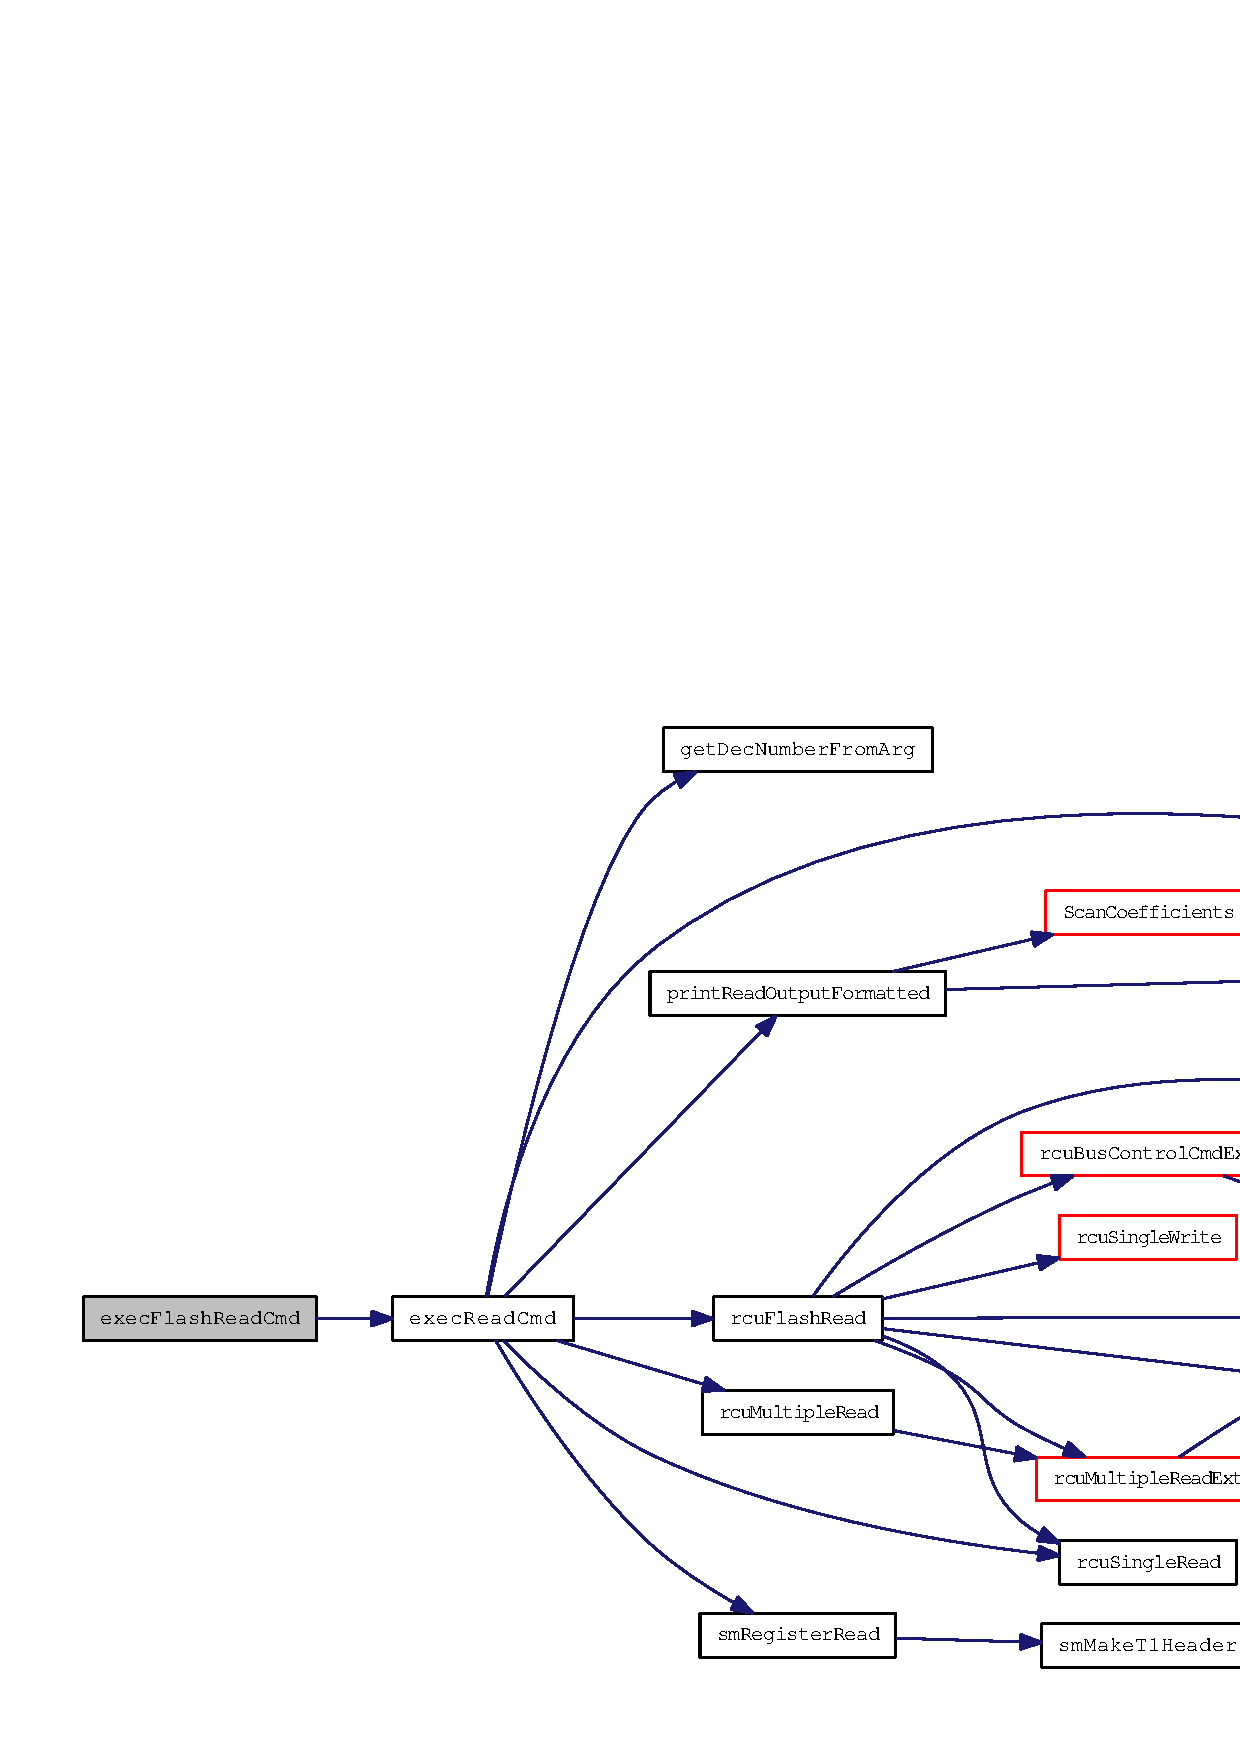
\includegraphics[width=390pt]{cmdInterpreter_8c_0069fb7612546c23d35da357dd126984_cgraph}
\end{center}
\end{figure}
\hypertarget{cmdInterpreter_8c_5df910c822508a5979806ec5d6548d65}{
\index{cmdInterpreter.c@{cmd\-Interpreter.c}!execFlashVerifyCmd@{execFlashVerifyCmd}}
\index{execFlashVerifyCmd@{execFlashVerifyCmd}!cmdInterpreter.c@{cmd\-Interpreter.c}}
\subsubsection[execFlashVerifyCmd]{\setlength{\rightskip}{0pt plus 5cm}int exec\-Flash\-Verify\-Cmd (const char $\ast$ {\em current\-Arg}, const char $\ast$$\ast$ {\em array\-Arg}, int {\em i\-Nof\-Args}, void $\ast$ {\em p\-User}, FILE $\ast$ {\em p\-Out})}}
\label{cmdInterpreter_8c_5df910c822508a5979806ec5d6548d65}




Definition at line 1704 of file cmd\-Interpreter.c.

References exec\-Write\-Cmd().

Here is the call graph for this function:\begin{figure}[H]
\begin{center}
\leavevmode
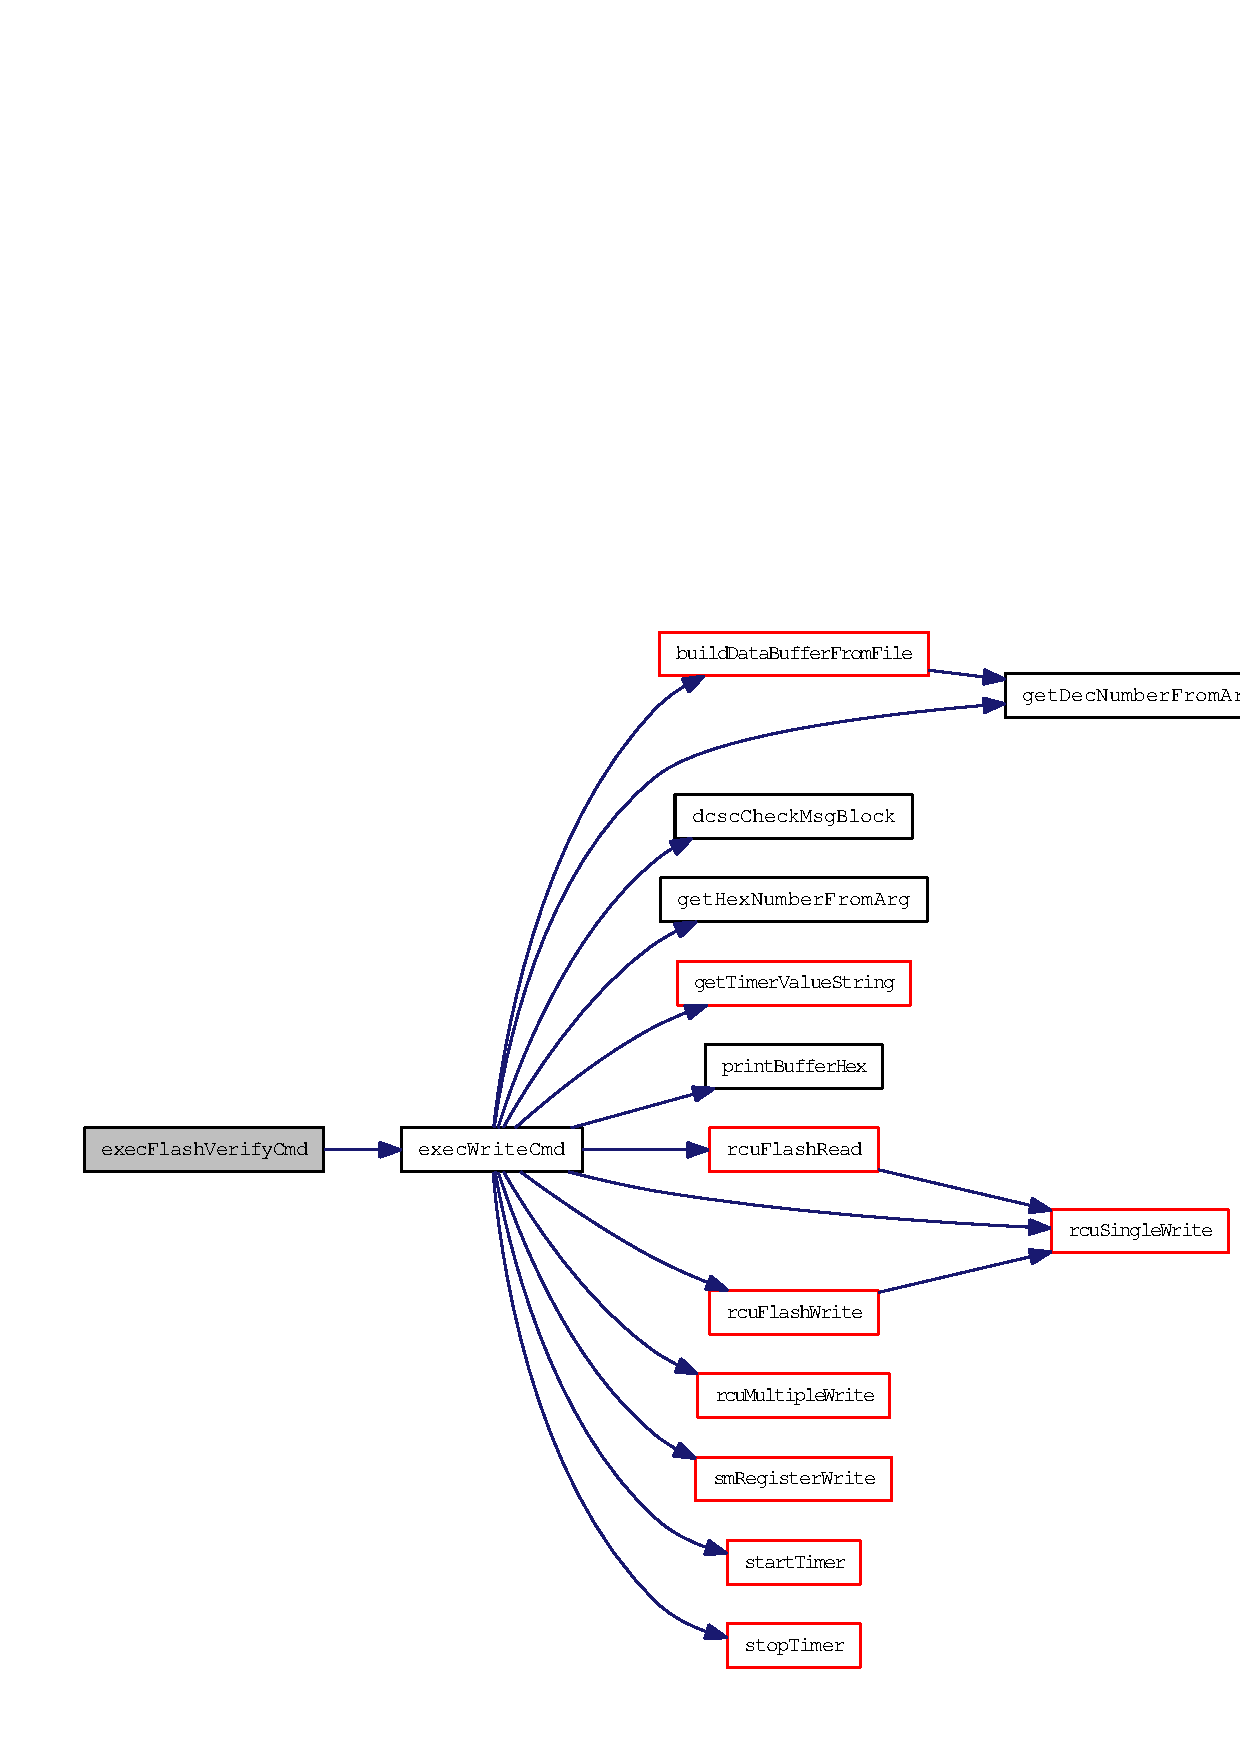
\includegraphics[width=308pt]{cmdInterpreter_8c_5df910c822508a5979806ec5d6548d65_cgraph}
\end{center}
\end{figure}
\hypertarget{cmdInterpreter_8c_765eadf200d9f408461f7469c791d22c}{
\index{cmdInterpreter.c@{cmd\-Interpreter.c}!execFlashWriteCmd@{execFlashWriteCmd}}
\index{execFlashWriteCmd@{execFlashWriteCmd}!cmdInterpreter.c@{cmd\-Interpreter.c}}
\subsubsection[execFlashWriteCmd]{\setlength{\rightskip}{0pt plus 5cm}int exec\-Flash\-Write\-Cmd (const char $\ast$ {\em current\-Arg}, const char $\ast$$\ast$ {\em array\-Arg}, int {\em i\-Nof\-Args}, void $\ast$ {\em p\-User}, FILE $\ast$ {\em p\-Out})}}
\label{cmdInterpreter_8c_765eadf200d9f408461f7469c791d22c}




Definition at line 1697 of file cmd\-Interpreter.c.

References exec\-Write\-Cmd().

Here is the call graph for this function:\begin{figure}[H]
\begin{center}
\leavevmode
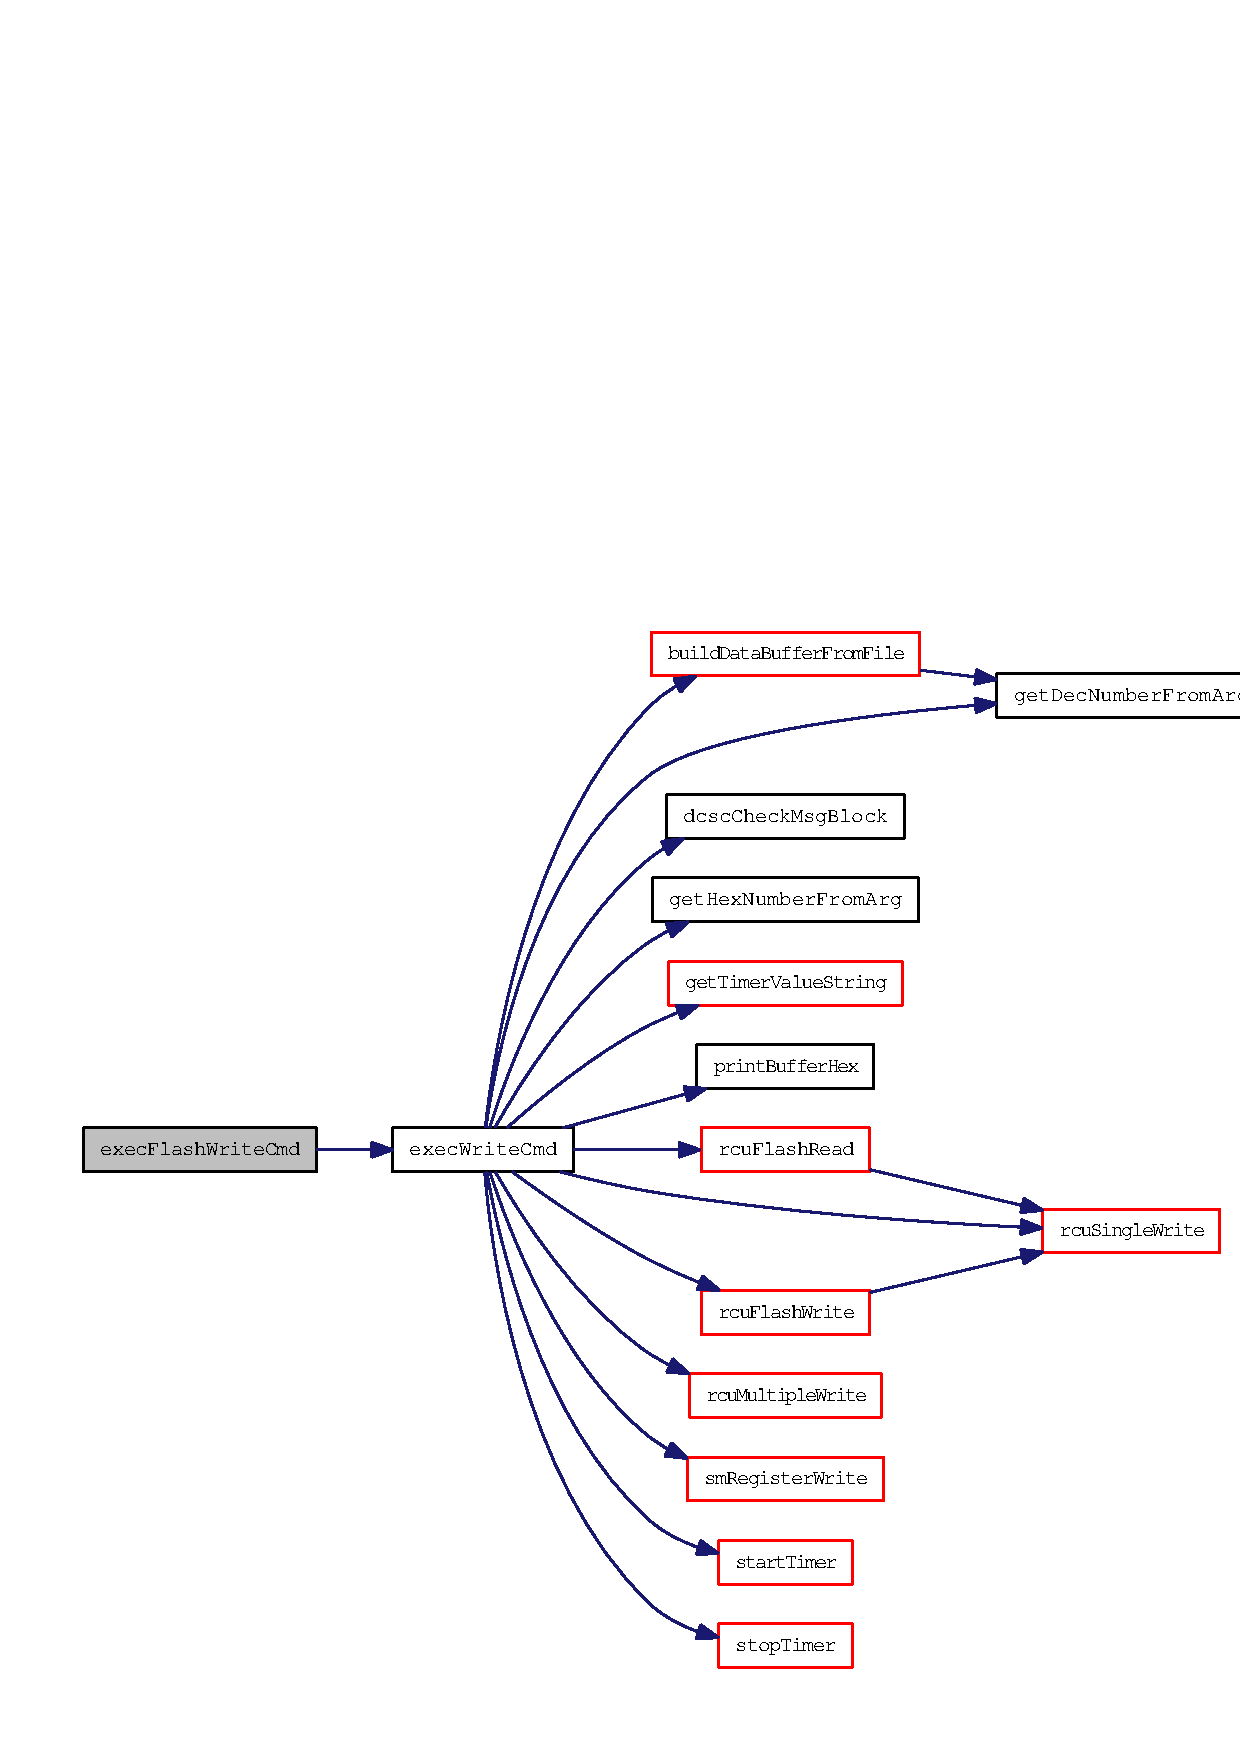
\includegraphics[width=306pt]{cmdInterpreter_8c_765eadf200d9f408461f7469c791d22c_cgraph}
\end{center}
\end{figure}
\hypertarget{cmdInterpreter_8c_a7c39db1bcd241c2ae5f259c0281abb6}{
\index{cmdInterpreter.c@{cmd\-Interpreter.c}!execReadCmd@{execReadCmd}}
\index{execReadCmd@{execReadCmd}!cmdInterpreter.c@{cmd\-Interpreter.c}}
\subsubsection[execReadCmd]{\setlength{\rightskip}{0pt plus 5cm}int exec\-Read\-Cmd (const char $\ast$$\ast$ {\em array\-Arg}, int {\em i\-Nof\-Args}, int {\em i\-Mode})}}
\label{cmdInterpreter_8c_a7c39db1bcd241c2ae5f259c0281abb6}




Definition at line 1153 of file cmd\-Interpreter.c.

References get\-Dec\-Number\-From\-Arg(), get\-Hex\-Number\-From\-Arg(), print\-Read\-Output\-Formatted(), rcu\-Flash\-Read(), rcu\-Multiple\-Read(), rcu\-Single\-Read(), and sm\-Register\-Read().

Referenced by exec\-Flash\-Read\-Cmd(), exec\-Sm\-Read\-Reg(), and execute\-Main\-Commands().

Here is the call graph for this function:\begin{figure}[H]
\begin{center}
\leavevmode
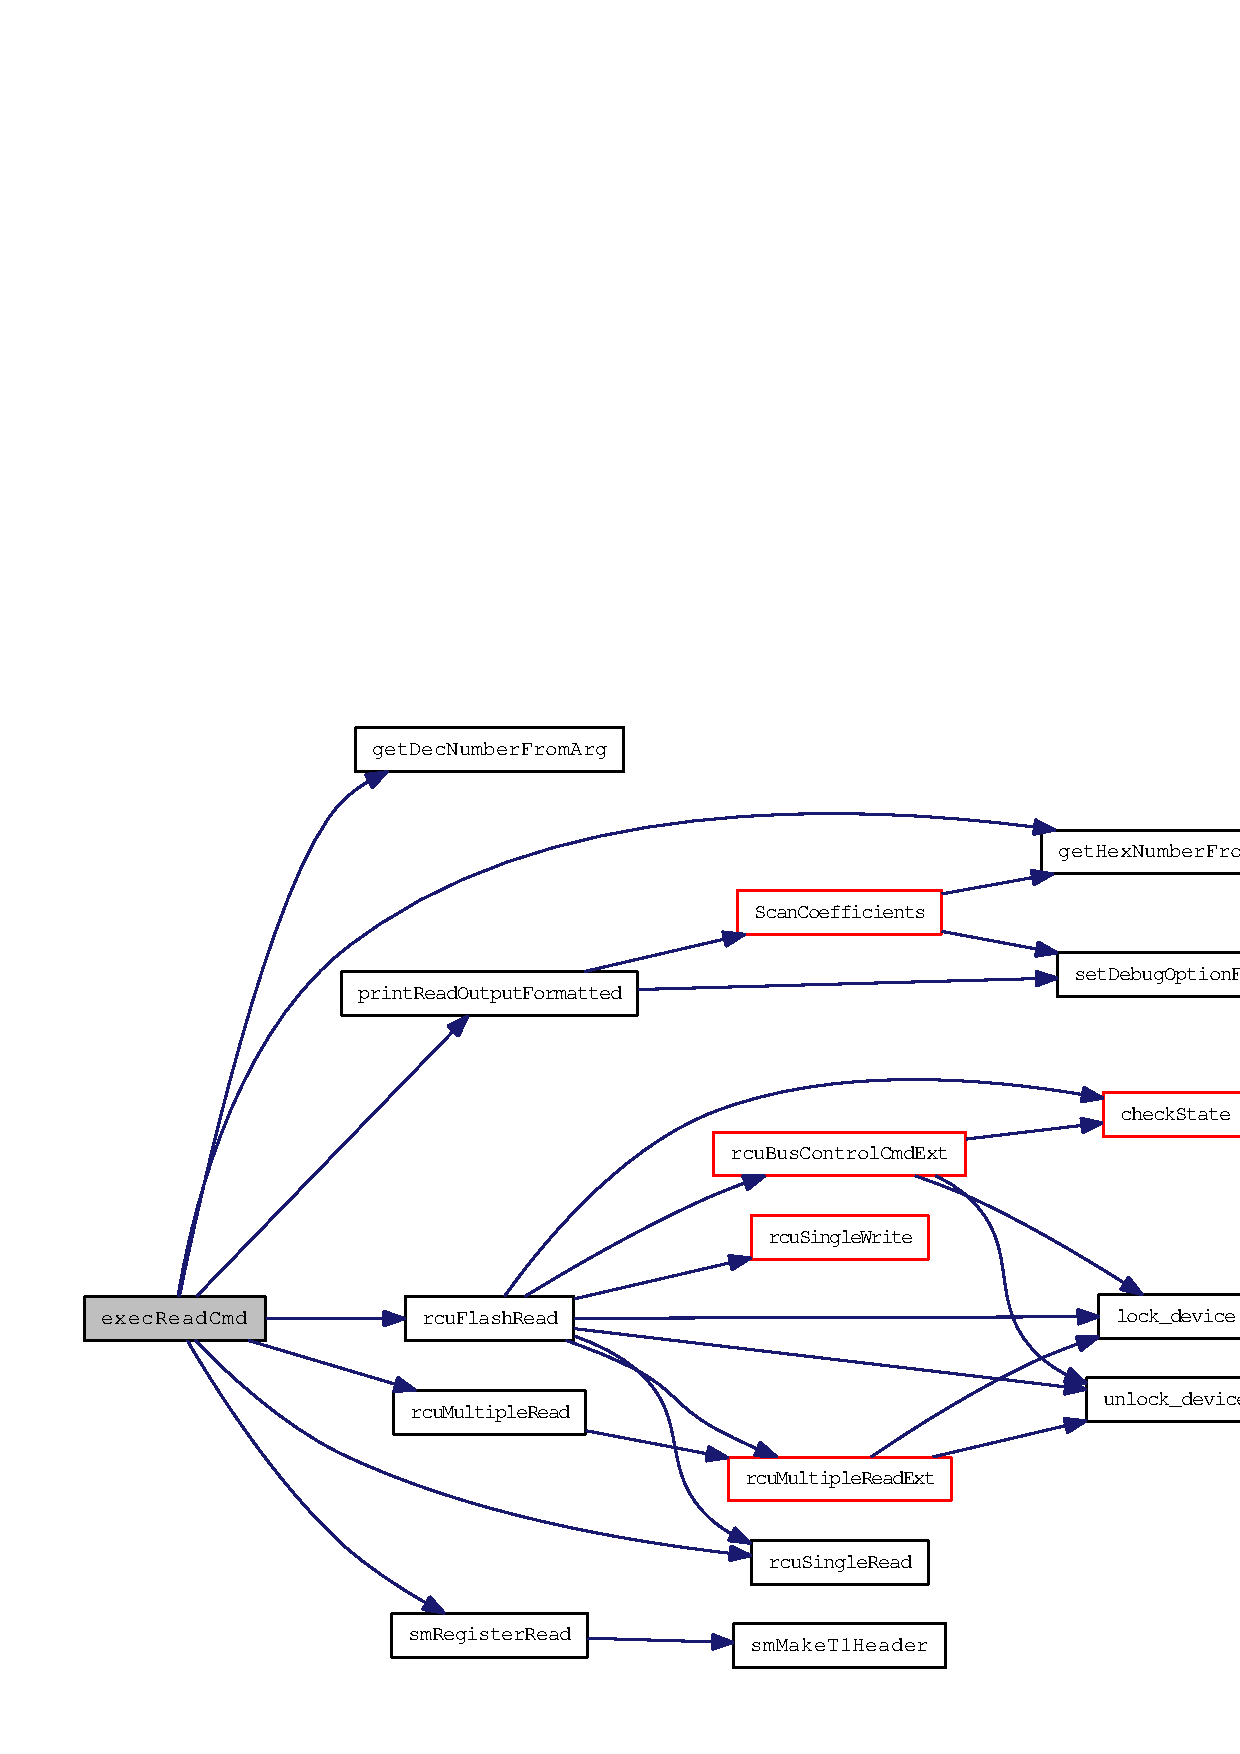
\includegraphics[width=316pt]{cmdInterpreter_8c_a7c39db1bcd241c2ae5f259c0281abb6_cgraph}
\end{center}
\end{figure}
\hypertarget{cmdInterpreter_8c_371d348f7b5d98c0ad4e7d6d20deb65c}{
\index{cmdInterpreter.c@{cmd\-Interpreter.c}!execRegReadCmd@{execRegReadCmd}}
\index{execRegReadCmd@{execRegReadCmd}!cmdInterpreter.c@{cmd\-Interpreter.c}}
\subsubsection[execRegReadCmd]{\setlength{\rightskip}{0pt plus 5cm}int exec\-Reg\-Read\-Cmd (const char $\ast$ {\em current\-Arg}, const char $\ast$$\ast$ {\em array\-Arg}, int {\em i\-Nof\-Args}, void $\ast$ {\em p\-User}, FILE $\ast$ {\em p\-Out})}}
\label{cmdInterpreter_8c_371d348f7b5d98c0ad4e7d6d20deb65c}




Definition at line 1801 of file cmd\-Interpreter.c.

References get\-Dec\-Number\-From\-Arg(), and msg\-Buf\-Read\-Register().

Here is the call graph for this function:\begin{figure}[H]
\begin{center}
\leavevmode
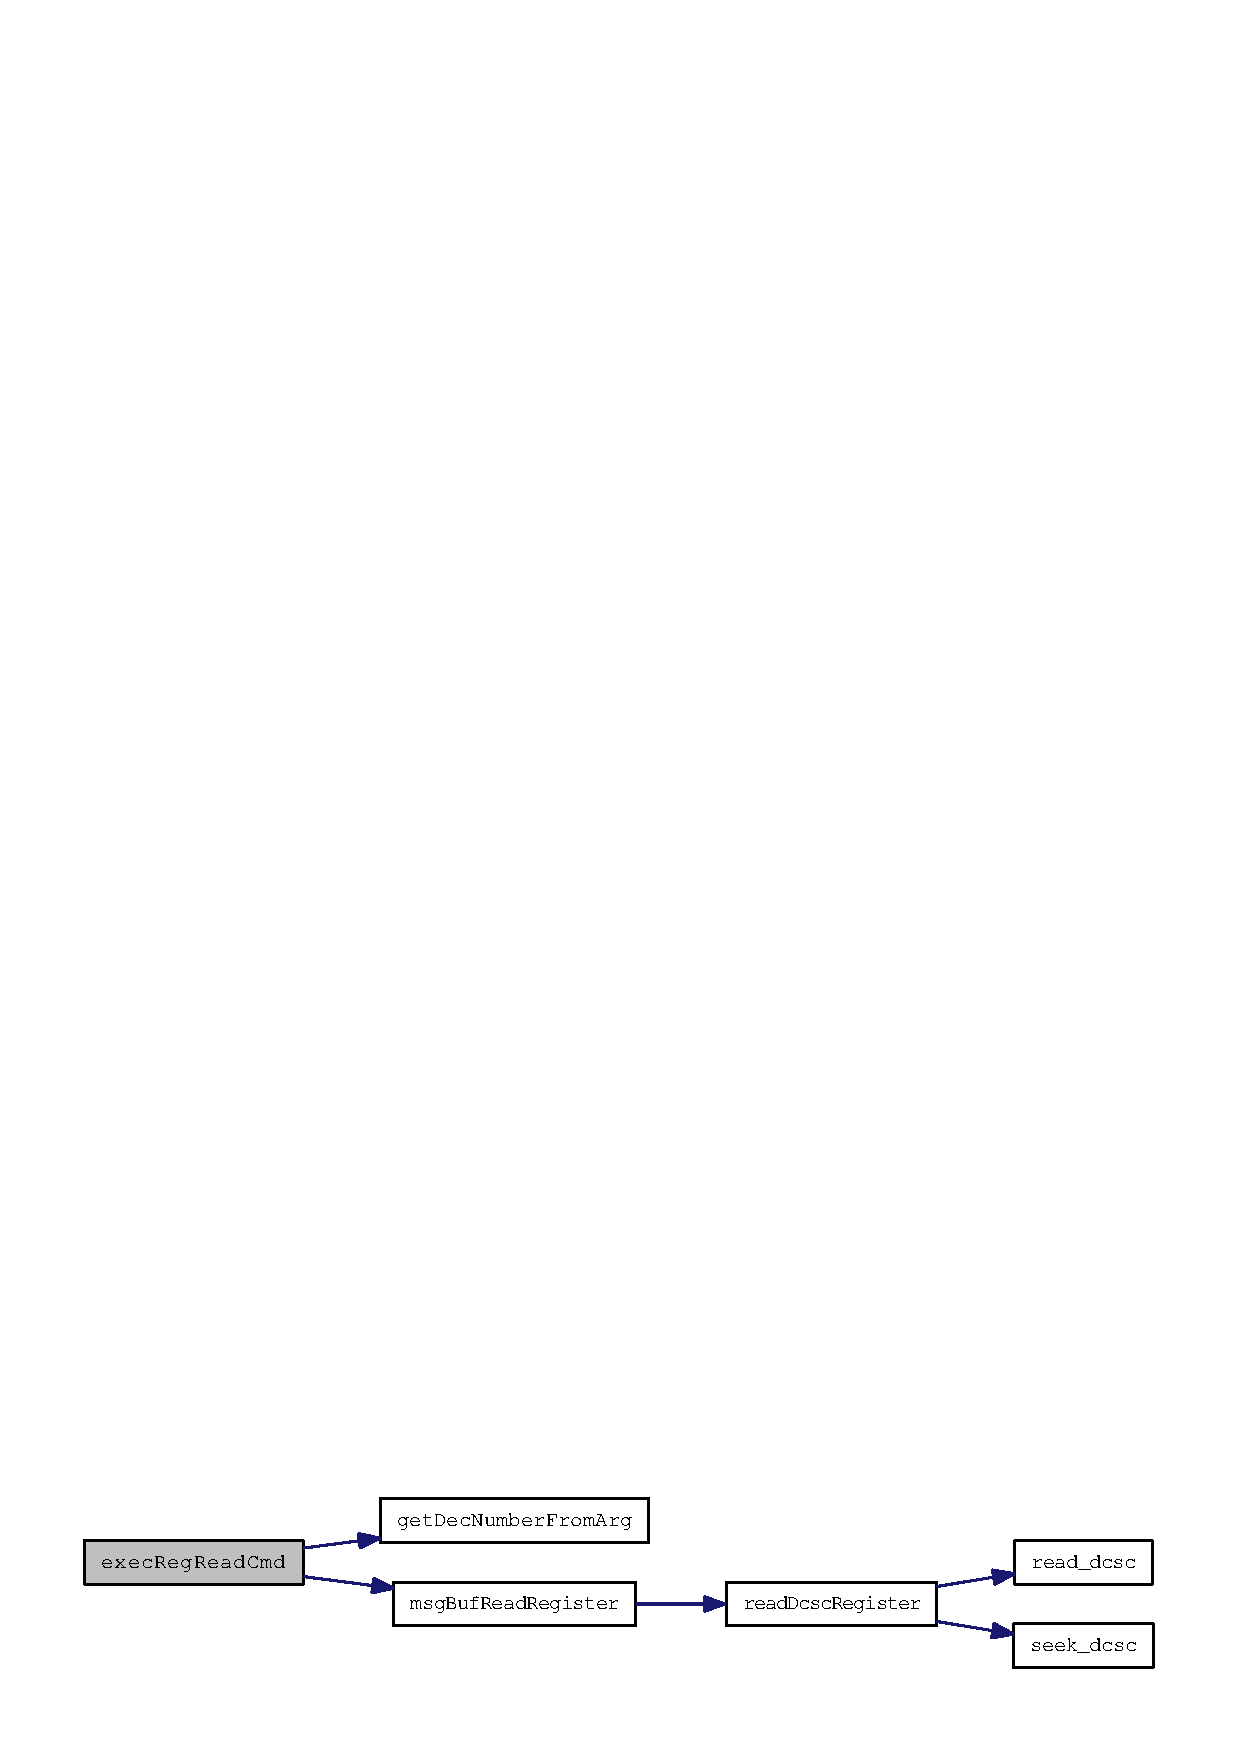
\includegraphics[width=279pt]{cmdInterpreter_8c_371d348f7b5d98c0ad4e7d6d20deb65c_cgraph}
\end{center}
\end{figure}
\hypertarget{cmdInterpreter_8c_72ffcd5a8ec94bc388af9b6d9781f5de}{
\index{cmdInterpreter.c@{cmd\-Interpreter.c}!execRegWriteCmd@{execRegWriteCmd}}
\index{execRegWriteCmd@{execRegWriteCmd}!cmdInterpreter.c@{cmd\-Interpreter.c}}
\subsubsection[execRegWriteCmd]{\setlength{\rightskip}{0pt plus 5cm}int exec\-Reg\-Write\-Cmd (const char $\ast$ {\em current\-Arg}, const char $\ast$$\ast$ {\em array\-Arg}, int {\em i\-Nof\-Args}, void $\ast$ {\em p\-User}, FILE $\ast$ {\em p\-Out})}}
\label{cmdInterpreter_8c_72ffcd5a8ec94bc388af9b6d9781f5de}




Definition at line 1785 of file cmd\-Interpreter.c.

References get\-Dec\-Number\-From\-Arg(), get\-Hex\-Number\-From\-Arg(), and msg\-Buf\-Write\-Register().

Here is the call graph for this function:\begin{figure}[H]
\begin{center}
\leavevmode
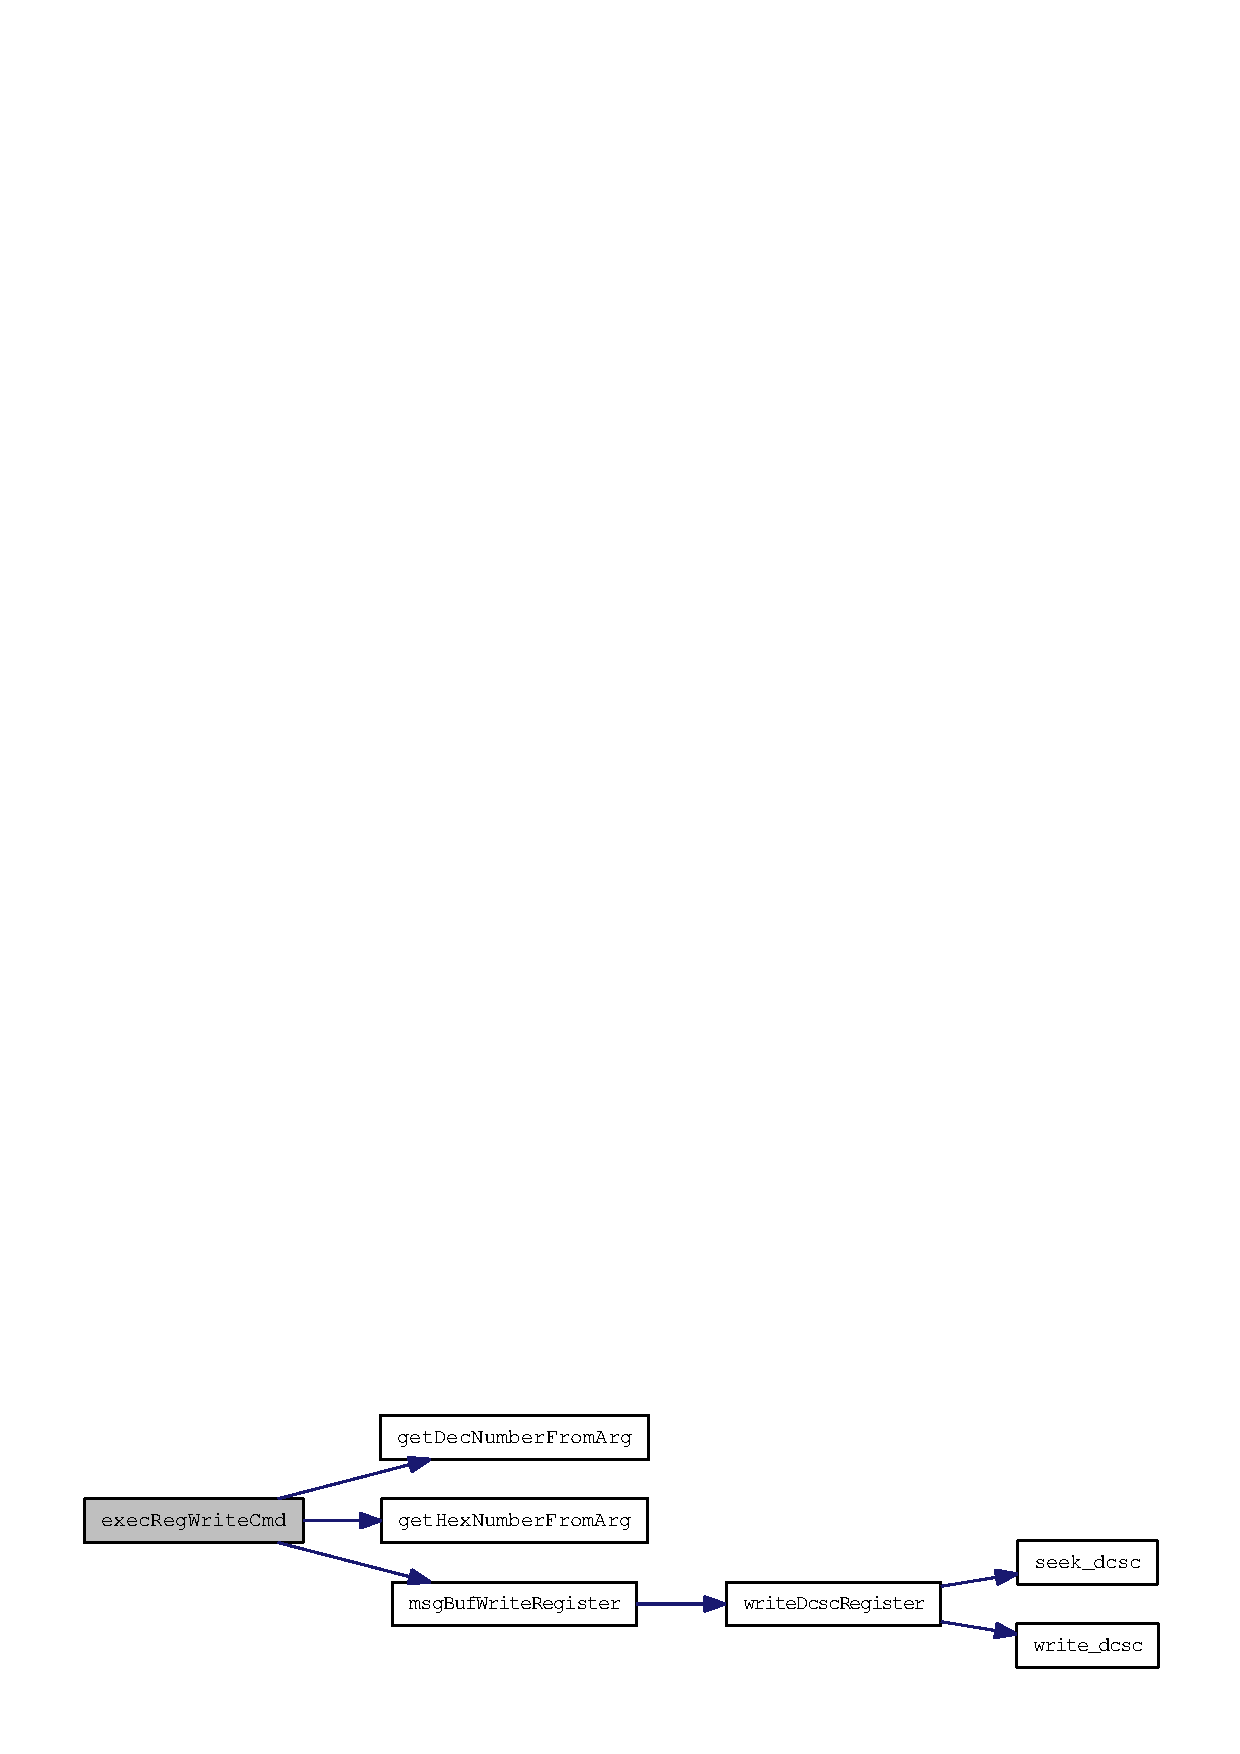
\includegraphics[width=280pt]{cmdInterpreter_8c_72ffcd5a8ec94bc388af9b6d9781f5de_cgraph}
\end{center}
\end{figure}
\hypertarget{cmdInterpreter_8c_acf8d85528167524bef8a5e23b9ffd99}{
\index{cmdInterpreter.c@{cmd\-Interpreter.c}!execSmReadReg@{execSmReadReg}}
\index{execSmReadReg@{execSmReadReg}!cmdInterpreter.c@{cmd\-Interpreter.c}}
\subsubsection[execSmReadReg]{\setlength{\rightskip}{0pt plus 5cm}int exec\-Sm\-Read\-Reg (const char $\ast$ {\em current\-Arg}, const char $\ast$$\ast$ {\em array\-Arg}, int {\em i\-Nof\-Args}, void $\ast$ {\em p\-User}, FILE $\ast$ {\em p\-Out})}}
\label{cmdInterpreter_8c_acf8d85528167524bef8a5e23b9ffd99}




Definition at line 1753 of file cmd\-Interpreter.c.

References exec\-Read\-Cmd().

Here is the call graph for this function:\begin{figure}[H]
\begin{center}
\leavevmode
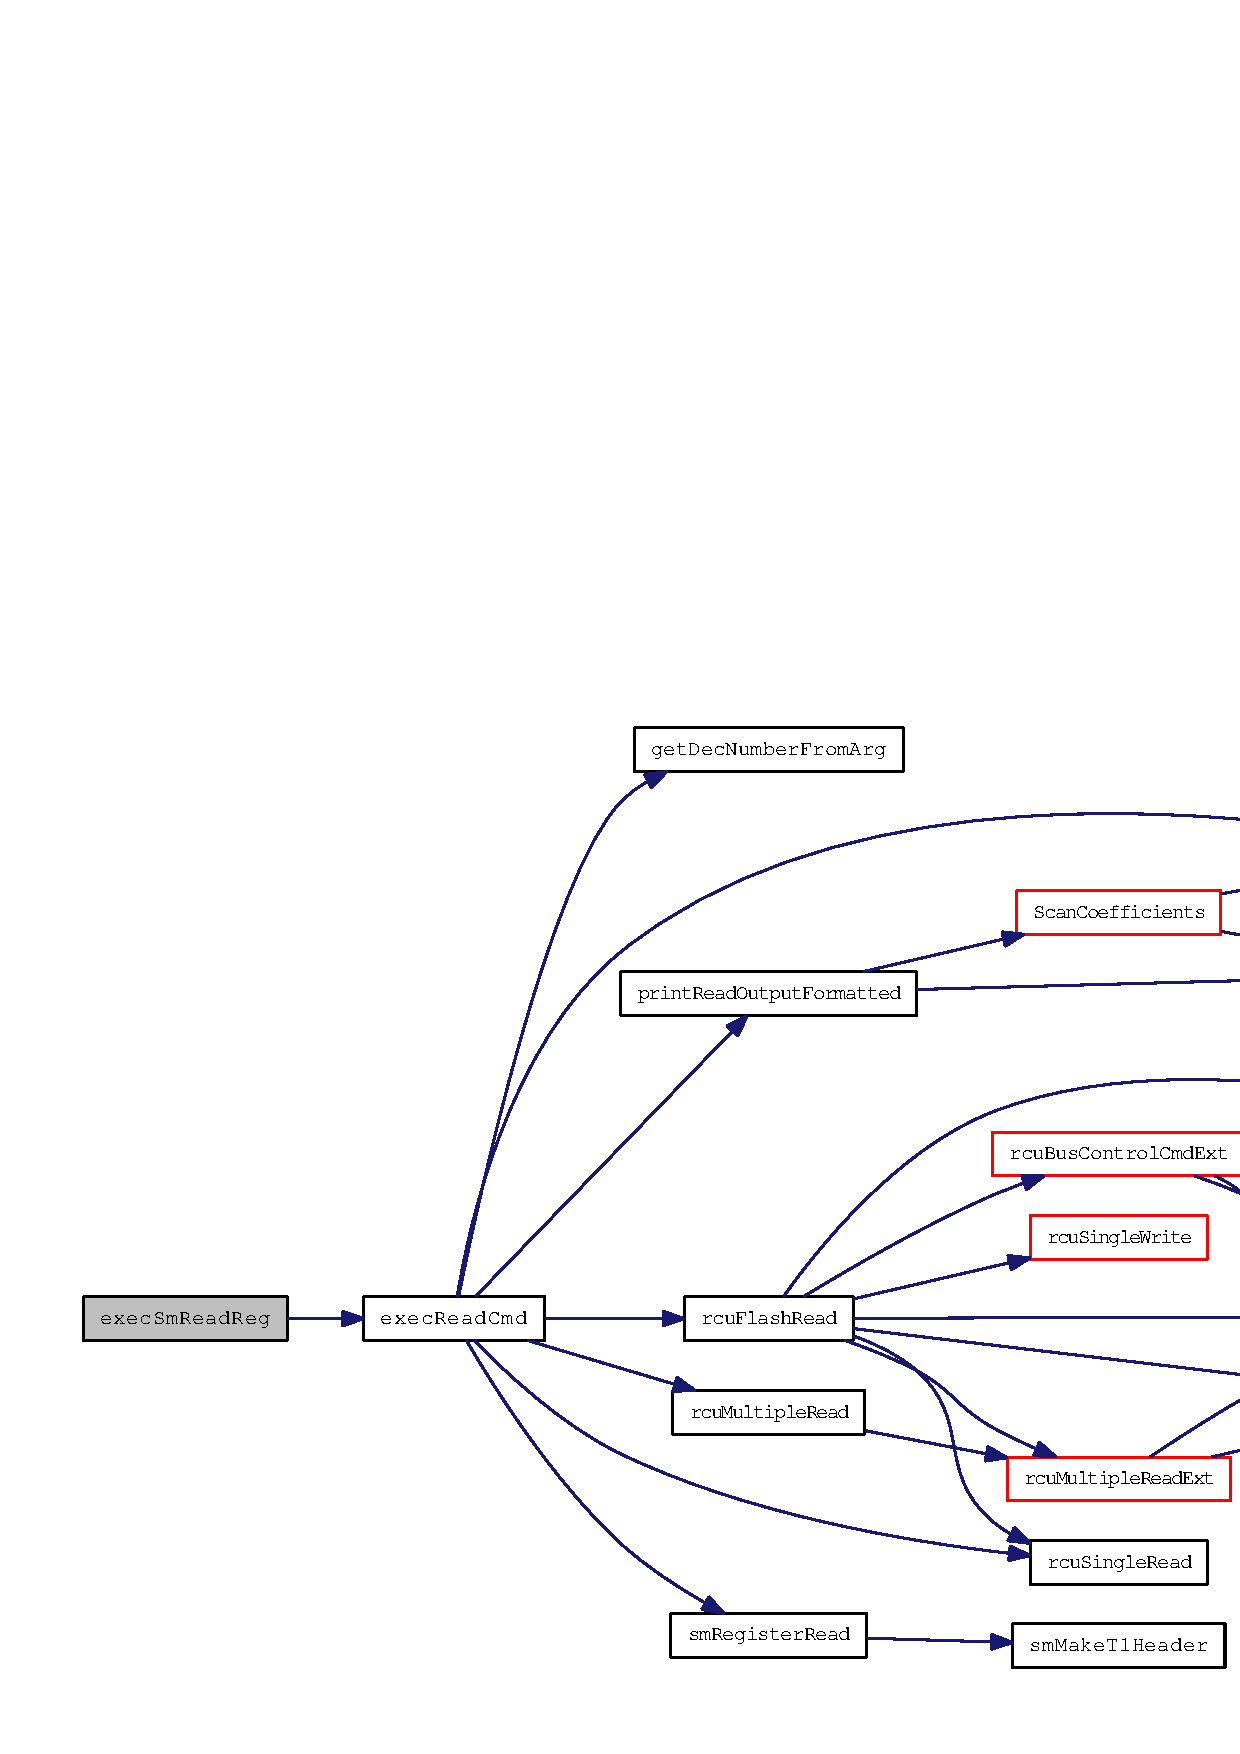
\includegraphics[width=383pt]{cmdInterpreter_8c_acf8d85528167524bef8a5e23b9ffd99_cgraph}
\end{center}
\end{figure}
\hypertarget{cmdInterpreter_8c_a8f5aca148fba0272ac3acfee150f651}{
\index{cmdInterpreter.c@{cmd\-Interpreter.c}!execSmWriteReg@{execSmWriteReg}}
\index{execSmWriteReg@{execSmWriteReg}!cmdInterpreter.c@{cmd\-Interpreter.c}}
\subsubsection[execSmWriteReg]{\setlength{\rightskip}{0pt plus 5cm}int exec\-Sm\-Write\-Reg (const char $\ast$ {\em current\-Arg}, const char $\ast$$\ast$ {\em array\-Arg}, int {\em i\-Nof\-Args}, void $\ast$ {\em p\-User}, FILE $\ast$ {\em p\-Out})}}
\label{cmdInterpreter_8c_a8f5aca148fba0272ac3acfee150f651}




Definition at line 1746 of file cmd\-Interpreter.c.

References exec\-Write\-Cmd().

Here is the call graph for this function:\begin{figure}[H]
\begin{center}
\leavevmode
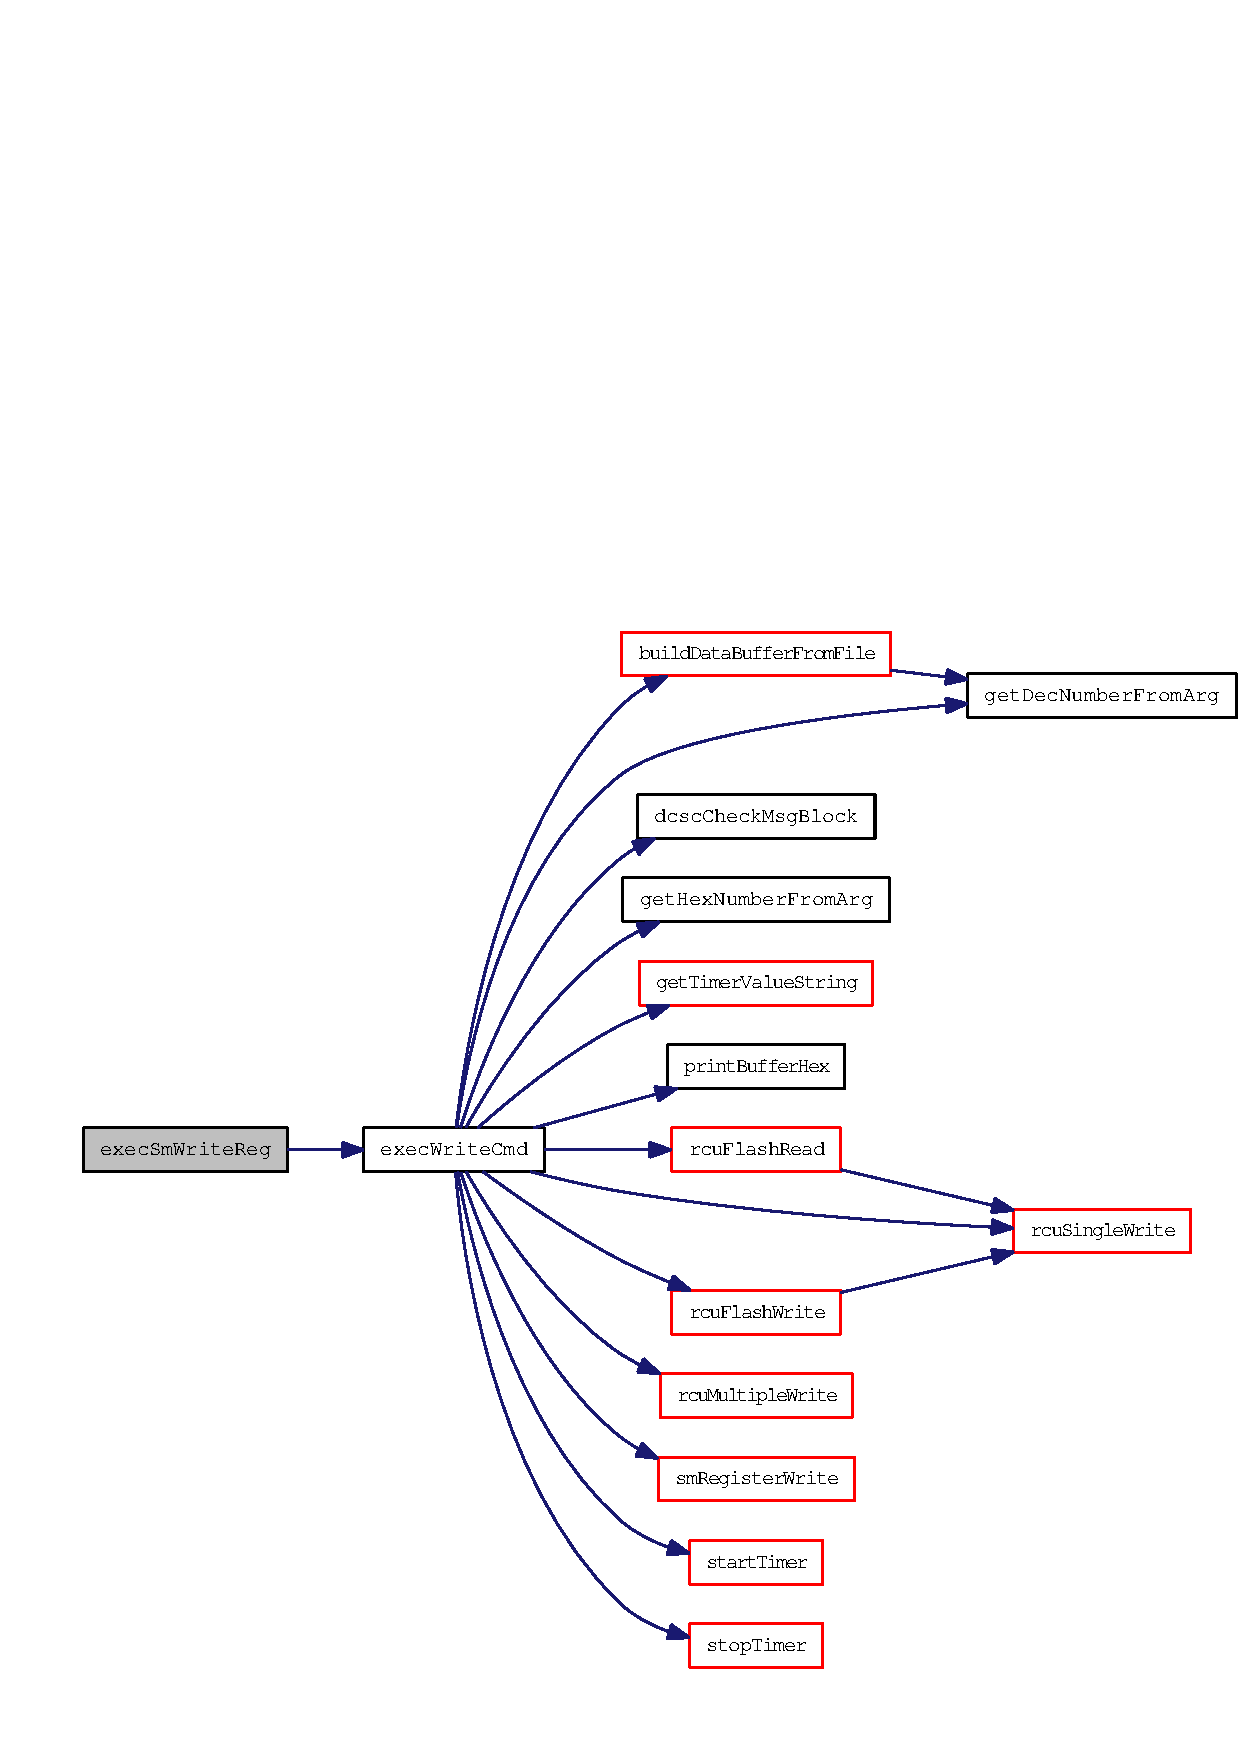
\includegraphics[width=299pt]{cmdInterpreter_8c_a8f5aca148fba0272ac3acfee150f651_cgraph}
\end{center}
\end{figure}
\hypertarget{cmdInterpreter_8c_54cbd6e4f4a91310f0c408dc5c6b413d}{
\index{cmdInterpreter.c@{cmd\-Interpreter.c}!executeCommandArgs@{executeCommandArgs}}
\index{executeCommandArgs@{executeCommandArgs}!cmdInterpreter.c@{cmd\-Interpreter.c}}
\subsubsection[executeCommandArgs]{\setlength{\rightskip}{0pt plus 5cm}int execute\-Command\-Args (int {\em i\-Nof\-Args}, const char $\ast$$\ast$ {\em array\-Arg})}}
\label{cmdInterpreter_8c_54cbd6e4f4a91310f0c408dc5c6b413d}




Definition at line 1892 of file cmd\-Interpreter.c.

References main\-Commands, mr\-Shell\-Prim\-Clone\-Def(), and Scan\-Arguments().

Referenced by execute\-Command\-Line(), and main().

Here is the call graph for this function:\begin{figure}[H]
\begin{center}
\leavevmode
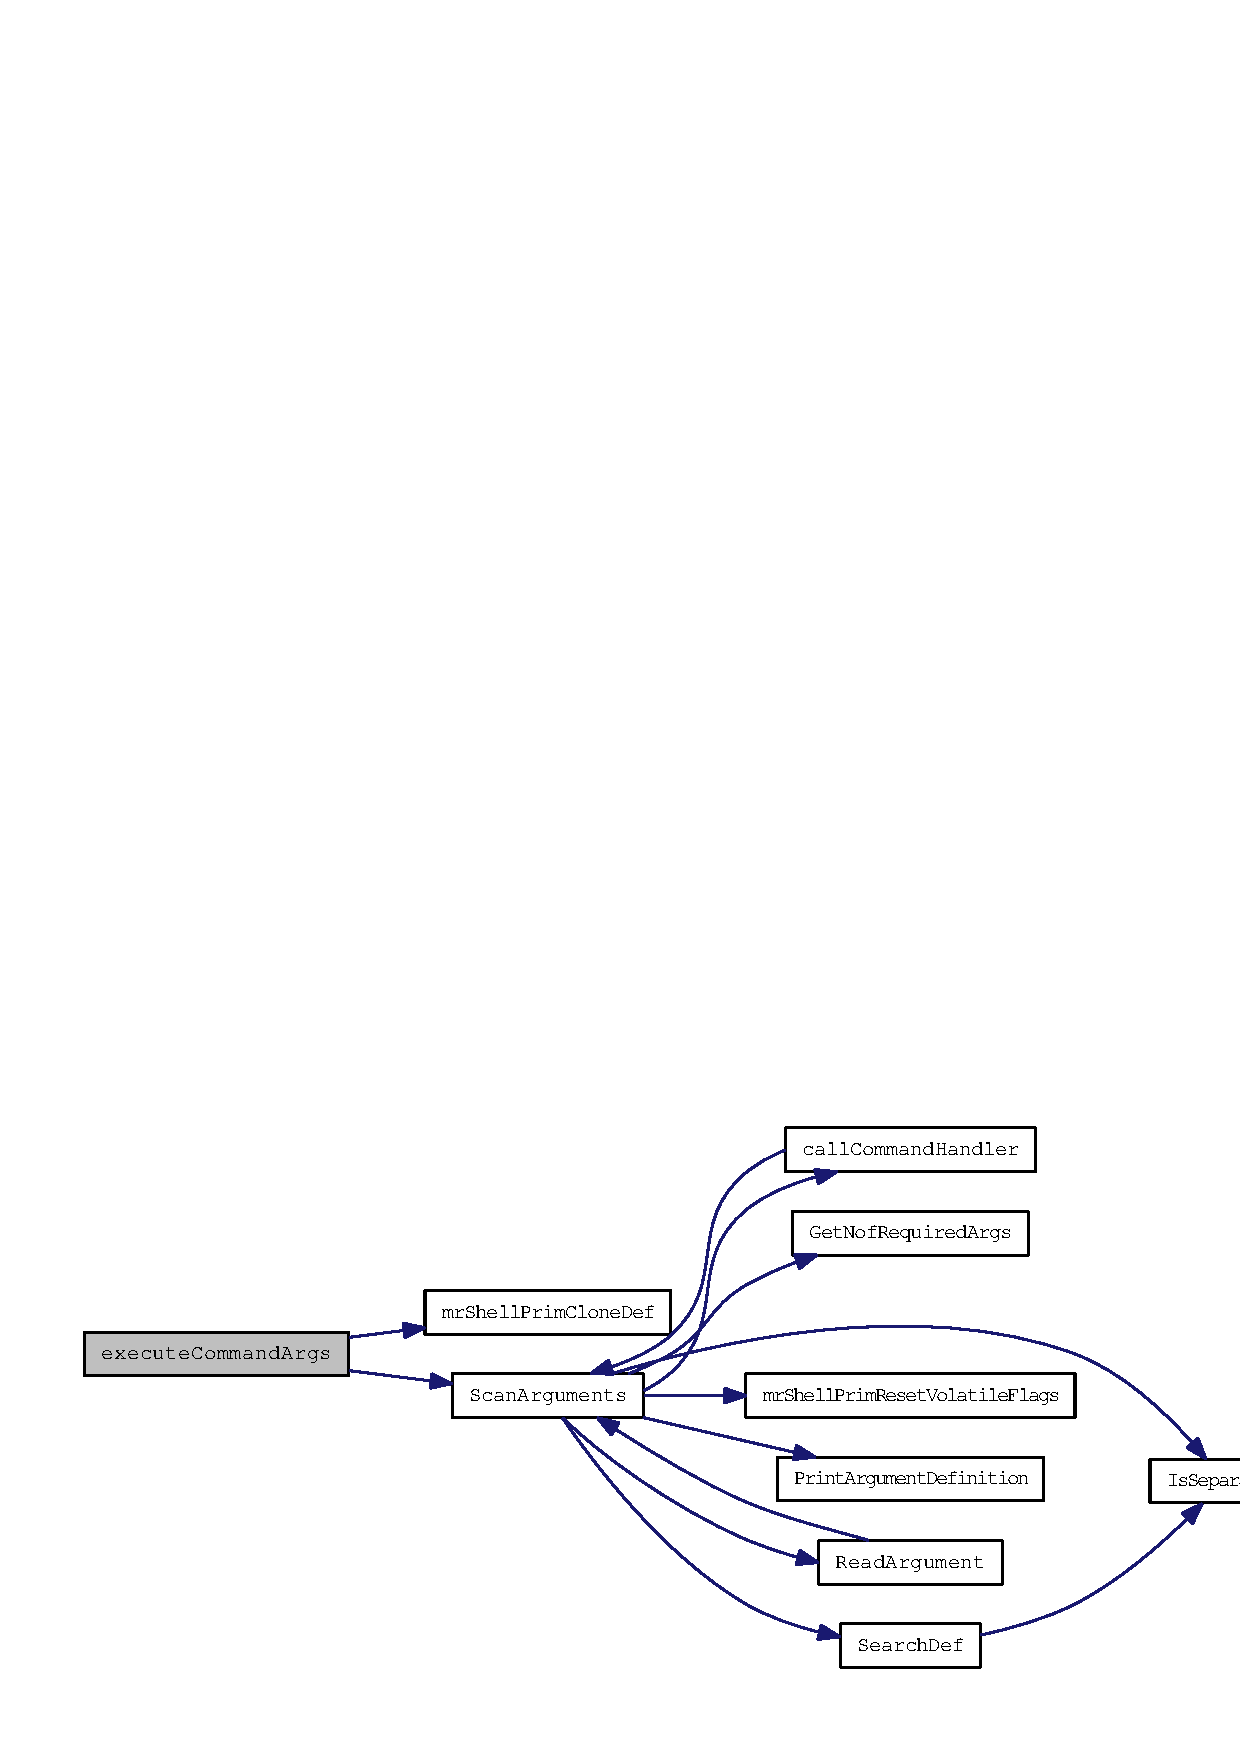
\includegraphics[width=313pt]{cmdInterpreter_8c_54cbd6e4f4a91310f0c408dc5c6b413d_cgraph}
\end{center}
\end{figure}
\hypertarget{cmdInterpreter_8c_48086998882e7d163126de4100aa12ac}{
\index{cmdInterpreter.c@{cmd\-Interpreter.c}!executeCommandLine@{executeCommandLine}}
\index{executeCommandLine@{executeCommandLine}!cmdInterpreter.c@{cmd\-Interpreter.c}}
\subsubsection[executeCommandLine]{\setlength{\rightskip}{0pt plus 5cm}int execute\-Command\-Line (char $\ast$ {\em p\-Cmd\-Line})}}
\label{cmdInterpreter_8c_48086998882e7d163126de4100aa12ac}




Definition at line 1904 of file cmd\-Interpreter.c.

References build\-Arguments\-From\-Command\-Line(), DBG\_\-ARGUMENT\_\-CONVERT, execute\-Command\-Args(), and set\-Debug\-Option\-Flag().

Referenced by exec\-Batch(), and main().

Here is the call graph for this function:\begin{figure}[H]
\begin{center}
\leavevmode
\includegraphics[width=273pt]{cmdInterpreter_8c_48086998882e7d163126de4100aa12ac_cgraph}
\end{center}
\end{figure}
\hypertarget{cmdInterpreter_8c_11ec76f8e60016409f2f33d10c70ef7e}{
\index{cmdInterpreter.c@{cmd\-Interpreter.c}!executeMainCommands@{executeMainCommands}}
\index{executeMainCommands@{executeMainCommands}!cmdInterpreter.c@{cmd\-Interpreter.c}}
\subsubsection[executeMainCommands]{\setlength{\rightskip}{0pt plus 5cm}int execute\-Main\-Commands (const char $\ast$ {\em current\-Arg}, const char $\ast$$\ast$ {\em array\-Arg}, int {\em i\-Nof\-Args}, void $\ast$ {\em p\-User}, FILE $\ast$ {\em p\-Out})}}
\label{cmdInterpreter_8c_11ec76f8e60016409f2f33d10c70ef7e}




Definition at line 1459 of file cmd\-Interpreter.c.

References clear\-Debug\-Option\-Flag(), clear\-MRTimer\-Debug\-Flag(), CMD\_\-STRING\_\-MRT\_\-DEBUG, CMD\_\-STRING\_\-PROFILE, DBG\_\-ARGUMENT\_\-CONVERT, DBG\_\-DEFAULT, exec\-Batch(), exec\-Read\-Cmd(), exec\-Write\-Cmd(), g\_\-profiling, get\-Dec\-Number\-From\-Arg(), get\-Hex\-Number\-From\-Arg(), print\-Batch\-Proc\-Help(), print\-Debug\-Help(), print\-Help(), print\-Read\-Help(), read\-Time(), set\-Debug\-Option\-Flag(), set\-Debug\-Options(), set\-MRTimer\-Debug\-Flag(), timed\-Wait(), and wait\-Condition().

Here is the call graph for this function:\begin{figure}[H]
\begin{center}
\leavevmode
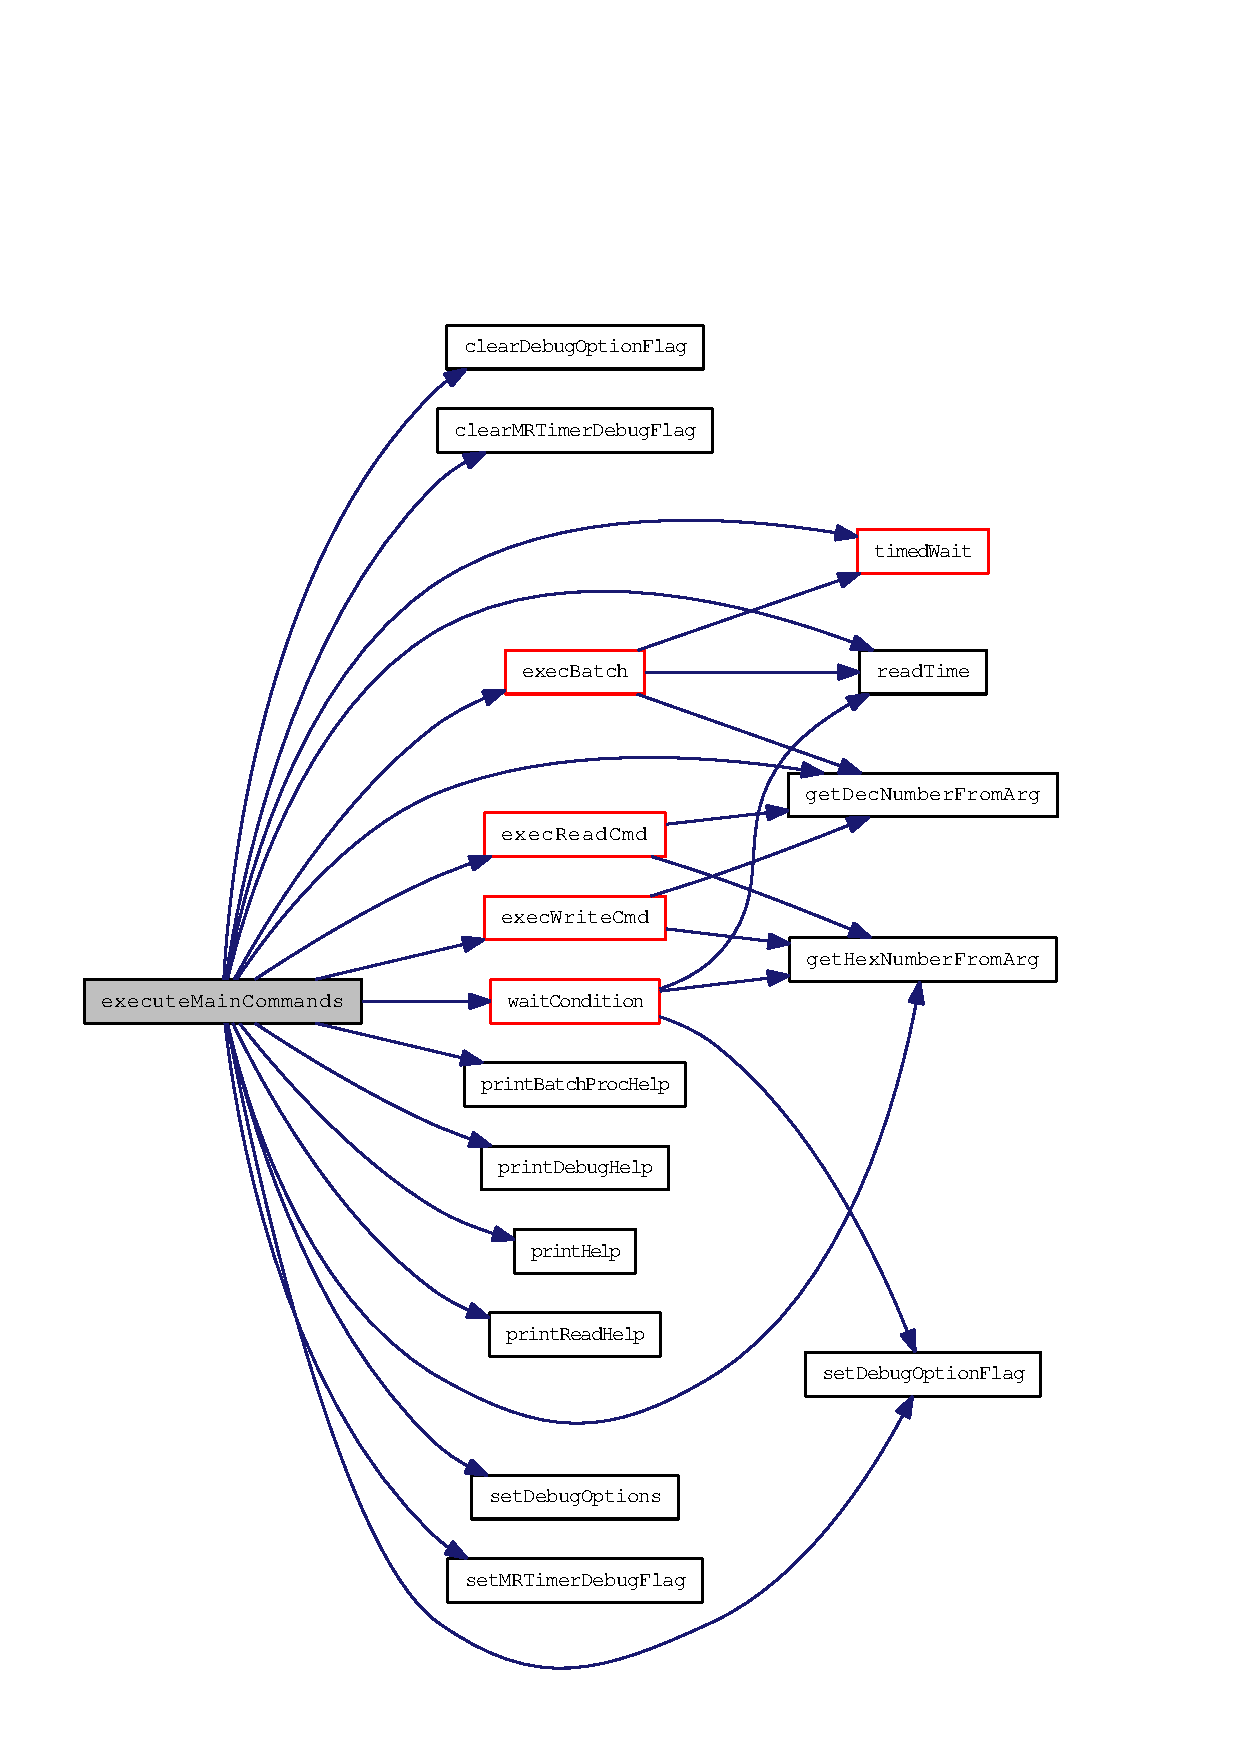
\includegraphics[width=256pt]{cmdInterpreter_8c_11ec76f8e60016409f2f33d10c70ef7e_cgraph}
\end{center}
\end{figure}
\hypertarget{cmdInterpreter_8c_6f67c6327e24c23440e0fdf83d06e41d}{
\index{cmdInterpreter.c@{cmd\-Interpreter.c}!execWriteCmd@{execWriteCmd}}
\index{execWriteCmd@{execWriteCmd}!cmdInterpreter.c@{cmd\-Interpreter.c}}
\subsubsection[execWriteCmd]{\setlength{\rightskip}{0pt plus 5cm}int exec\-Write\-Cmd (const char $\ast$$\ast$ {\em array\-Arg}, int {\em i\-Nof\-Args}, int {\em i\-Mode})}}
\label{cmdInterpreter_8c_6f67c6327e24c23440e0fdf83d06e41d}


execute the write command there are 3 argument formats, the argument array is scanned and interpreted according to: 1. 

address data 2. address count data 3. address \mbox{[}file options\mbox{]} filename count \begin{Desc}
\item[Parameters:]
\begin{description}
\item[{\em i\-Mode}]function modes\par
 0 normal msgbuffer write function\par
 1 compare of the MIB, debugging feature to compare MIB with a file\par
 2 flash write mode\par
 3 flash verify\par
 8 selectmap register write\par
 \end{description}
\end{Desc}


Definition at line 632 of file cmd\-Interpreter.c.

References build\-Data\-Buffer\-From\-File(), dcsc\-Check\-Msg\-Block(), g\_\-profiling, get\-Dec\-Number\-From\-Arg(), get\-Hex\-Number\-From\-Arg(), get\-Timer\-Value\-String(), print\-Buffer\-Hex(), rcu\-Flash\-Read(), rcu\-Flash\-Write(), rcu\-Multiple\-Write(), rcu\-Single\-Write(), sm\-Register\-Write(), start\-Timer(), and stop\-Timer().

Referenced by exec\-Flash\-Verify\-Cmd(), exec\-Flash\-Write\-Cmd(), exec\-Sm\-Write\-Reg(), and execute\-Main\-Commands().

Here is the call graph for this function:\begin{figure}[H]
\begin{center}
\leavevmode
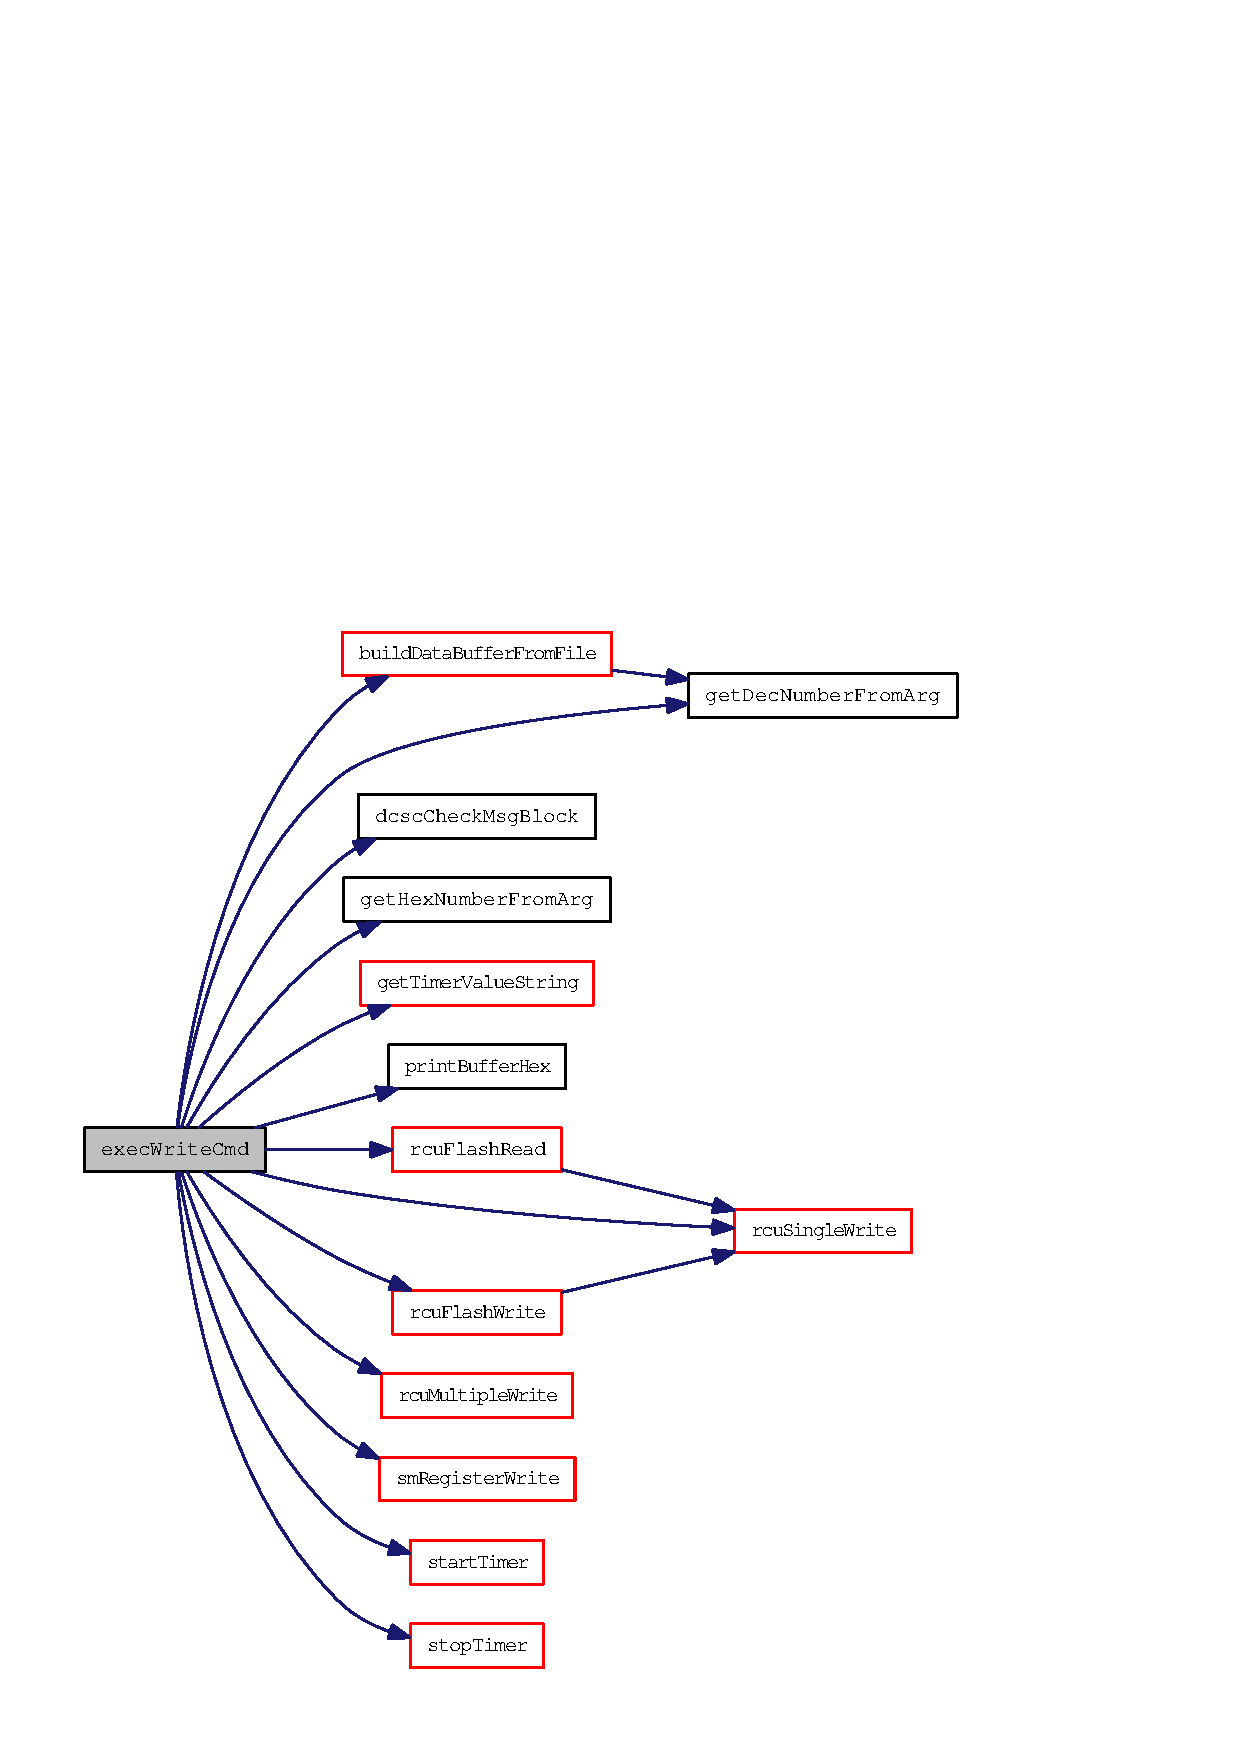
\includegraphics[width=232pt]{cmdInterpreter_8c_6f67c6327e24c23440e0fdf83d06e41d_cgraph}
\end{center}
\end{figure}
\hypertarget{cmdInterpreter_8c_c744cdcd05bdccf013ccbc82daa2282a}{
\index{cmdInterpreter.c@{cmd\-Interpreter.c}!printBatchProcHelp@{printBatchProcHelp}}
\index{printBatchProcHelp@{printBatchProcHelp}!cmdInterpreter.c@{cmd\-Interpreter.c}}
\subsubsection[printBatchProcHelp]{\setlength{\rightskip}{0pt plus 5cm}void print\-Batch\-Proc\-Help ()}}
\label{cmdInterpreter_8c_c744cdcd05bdccf013ccbc82daa2282a}




Definition at line 262 of file cmd\-Interpreter.c.

Referenced by execute\-Main\-Commands().\hypertarget{cmdInterpreter_8c_15843554cb32ffb674f4245cfe5ee524}{
\index{cmdInterpreter.c@{cmd\-Interpreter.c}!printDebugHelp@{printDebugHelp}}
\index{printDebugHelp@{printDebugHelp}!cmdInterpreter.c@{cmd\-Interpreter.c}}
\subsubsection[printDebugHelp]{\setlength{\rightskip}{0pt plus 5cm}void print\-Debug\-Help (int {\em i\-Level})}}
\label{cmdInterpreter_8c_15843554cb32ffb674f4245cfe5ee524}




Definition at line 173 of file cmd\-Interpreter.c.

References CHECK\_\-COMMAND\_\-BUFFER, DBG\_\-ARGUMENT\_\-CONVERT, DBG\_\-CHECK\_\-COMMAND, DBG\_\-DEFAULT, DBG\_\-FILE\_\-CONVERT, IGNORE\_\-BUFFER\_\-CHECK, PRINT\_\-COMMAND\_\-BUFFER, PRINT\_\-COMMAND\_\-RESULT, PRINT\_\-REGISTER\_\-ACCESS, PRINT\_\-RESULT\_\-BUFFER, PRINT\_\-RESULT\_\-HUMAN\_\-READABLE, and PRINT\_\-SPLIT\_\-DEBUG.

Referenced by execute\-Main\-Commands().\hypertarget{cmdInterpreter_8c_69279ab735c2dc7e0a73d9c0bfe44f20}{
\index{cmdInterpreter.c@{cmd\-Interpreter.c}!printFirmwareHelp@{printFirmwareHelp}}
\index{printFirmwareHelp@{printFirmwareHelp}!cmdInterpreter.c@{cmd\-Interpreter.c}}
\subsubsection[printFirmwareHelp]{\setlength{\rightskip}{0pt plus 5cm}int print\-Firmware\-Help ()}}
\label{cmdInterpreter_8c_69279ab735c2dc7e0a73d9c0bfe44f20}




Definition at line 1773 of file cmd\-Interpreter.c.\hypertarget{cmdInterpreter_8c_587fc3f8784e8339c998d9ca71bd7e12}{
\index{cmdInterpreter.c@{cmd\-Interpreter.c}!printFlashHelp@{printFlashHelp}}
\index{printFlashHelp@{printFlashHelp}!cmdInterpreter.c@{cmd\-Interpreter.c}}
\subsubsection[printFlashHelp]{\setlength{\rightskip}{0pt plus 5cm}int print\-Flash\-Help ()}}
\label{cmdInterpreter_8c_587fc3f8784e8339c998d9ca71bd7e12}




Definition at line 1677 of file cmd\-Interpreter.c.\hypertarget{cmdInterpreter_8c_f03f7609a66def2e7fae02a477c38d97}{
\index{cmdInterpreter.c@{cmd\-Interpreter.c}!printHelp@{printHelp}}
\index{printHelp@{printHelp}!cmdInterpreter.c@{cmd\-Interpreter.c}}
\subsubsection[printHelp]{\setlength{\rightskip}{0pt plus 5cm}int print\-Help ()}}
\label{cmdInterpreter_8c_f03f7609a66def2e7fae02a477c38d97}




Definition at line 198 of file cmd\-Interpreter.c.

Referenced by execute\-Main\-Commands().\hypertarget{cmdInterpreter_8c_ac3ae2fb745e63e33060d5c0b658f745}{
\index{cmdInterpreter.c@{cmd\-Interpreter.c}!printInfo@{printInfo}}
\index{printInfo@{printInfo}!cmdInterpreter.c@{cmd\-Interpreter.c}}
\subsubsection[printInfo]{\setlength{\rightskip}{0pt plus 5cm}int print\-Info ()}}
\label{cmdInterpreter_8c_ac3ae2fb745e63e33060d5c0b658f745}




Definition at line 164 of file cmd\-Interpreter.c.\hypertarget{cmdInterpreter_8c_17ba9ebf0687897855a7c95f19e99c3d}{
\index{cmdInterpreter.c@{cmd\-Interpreter.c}!printReadHelp@{printReadHelp}}
\index{printReadHelp@{printReadHelp}!cmdInterpreter.c@{cmd\-Interpreter.c}}
\subsubsection[printReadHelp]{\setlength{\rightskip}{0pt plus 5cm}void print\-Read\-Help ()}}
\label{cmdInterpreter_8c_17ba9ebf0687897855a7c95f19e99c3d}




Definition at line 240 of file cmd\-Interpreter.c.

Referenced by execute\-Main\-Commands().\hypertarget{cmdInterpreter_8c_e3bcc6695f3c41940a8ab1f428101f07}{
\index{cmdInterpreter.c@{cmd\-Interpreter.c}!printReadOutputFormatted@{printReadOutputFormatted}}
\index{printReadOutputFormatted@{printReadOutputFormatted}!cmdInterpreter.c@{cmd\-Interpreter.c}}
\subsubsection[printReadOutputFormatted]{\setlength{\rightskip}{0pt plus 5cm}int print\-Read\-Output\-Formatted (unsigned char $\ast$ {\em p\-Buffer}, int {\em i\-Buffer\-Size}, const char $\ast$ {\em p\-Format}, int {\em i\-Start\-Address}, FILE $\ast$ {\em fp})}}
\label{cmdInterpreter_8c_e3bcc6695f3c41940a8ab1f428101f07}




Definition at line 946 of file cmd\-Interpreter.c.

References DBG\_\-ARGUMENT\_\-CONVERT, INT\_\-RO\_\-MAX, Scan\-Coefficients(), set\-Debug\-Option\-Flag(), and UINT\_\-MAX.

Referenced by exec\-Read\-Cmd().

Here is the call graph for this function:\begin{figure}[H]
\begin{center}
\leavevmode
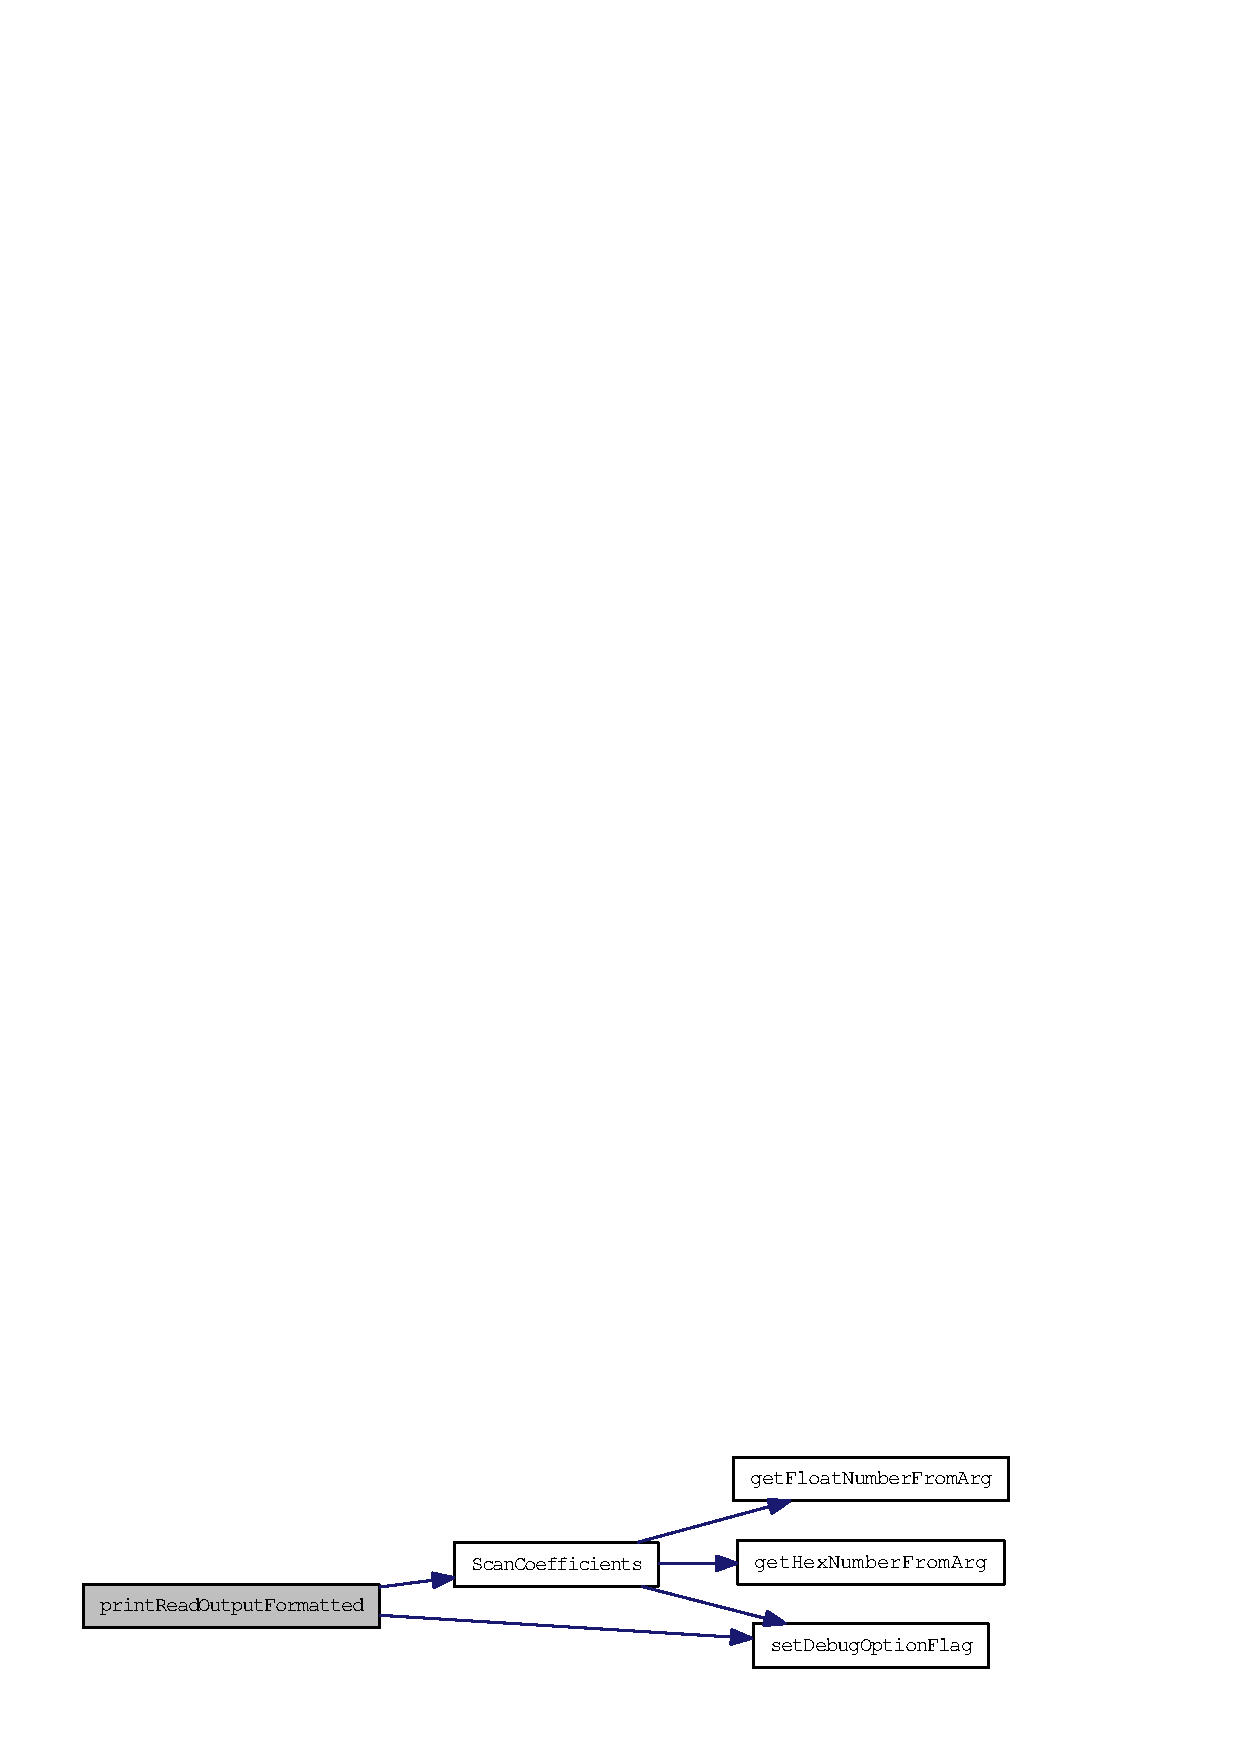
\includegraphics[width=244pt]{cmdInterpreter_8c_e3bcc6695f3c41940a8ab1f428101f07_cgraph}
\end{center}
\end{figure}
\hypertarget{cmdInterpreter_8c_76b0a4b334ee64eb25b1637d709deb92}{
\index{cmdInterpreter.c@{cmd\-Interpreter.c}!printSelectmapHelp@{printSelectmapHelp}}
\index{printSelectmapHelp@{printSelectmapHelp}!cmdInterpreter.c@{cmd\-Interpreter.c}}
\subsubsection[printSelectmapHelp]{\setlength{\rightskip}{0pt plus 5cm}int print\-Selectmap\-Help ()}}
\label{cmdInterpreter_8c_76b0a4b334ee64eb25b1637d709deb92}




Definition at line 1760 of file cmd\-Interpreter.c.\hypertarget{cmdInterpreter_8c_6ead18c93a106e1f1ba5871e908d9916}{
\index{cmdInterpreter.c@{cmd\-Interpreter.c}!readTime@{readTime}}
\index{readTime@{readTime}!cmdInterpreter.c@{cmd\-Interpreter.c}}
\subsubsection[readTime]{\setlength{\rightskip}{0pt plus 5cm}int read\-Time (const char $\ast$$\ast$ {\em array\-Arg}, int {\em i\-Nof\-Args}, int $\ast$ {\em p\-Sec}, int $\ast$ {\em p\-Musec})}}
\label{cmdInterpreter_8c_6ead18c93a106e1f1ba5871e908d9916}




Definition at line 273 of file cmd\-Interpreter.c.

Referenced by exec\-Batch(), execute\-Main\-Commands(), and wait\-Condition().\hypertarget{cmdInterpreter_8c_78a2282cf7d3dbf552e5f9876dba01cf}{
\index{cmdInterpreter.c@{cmd\-Interpreter.c}!ScanCoefficients@{ScanCoefficients}}
\index{ScanCoefficients@{ScanCoefficients}!cmdInterpreter.c@{cmd\-Interpreter.c}}
\subsubsection[ScanCoefficients]{\setlength{\rightskip}{0pt plus 5cm}int Scan\-Coefficients (const char $\ast$ {\em p\-Format}, float $\ast$ {\em pf\-M}, float $\ast$ {\em pf\-N}, \_\-\_\-u32 $\ast$ {\em p\-Mask})}}
\label{cmdInterpreter_8c_78a2282cf7d3dbf552e5f9876dba01cf}




Definition at line 862 of file cmd\-Interpreter.c.

References DBG\_\-ARGUMENT\_\-CONVERT, get\-Float\-Number\-From\-Arg(), get\-Hex\-Number\-From\-Arg(), and set\-Debug\-Option\-Flag().

Referenced by print\-Read\-Output\-Formatted().

Here is the call graph for this function:\begin{figure}[H]
\begin{center}
\leavevmode
\includegraphics[width=155pt]{cmdInterpreter_8c_78a2282cf7d3dbf552e5f9876dba01cf_cgraph}
\end{center}
\end{figure}
\hypertarget{cmdInterpreter_8c_ae37490e691f5b4d2c2e8f22713555da}{
\index{cmdInterpreter.c@{cmd\-Interpreter.c}!terminateBatchProcessing@{terminateBatchProcessing}}
\index{terminateBatchProcessing@{terminateBatchProcessing}!cmdInterpreter.c@{cmd\-Interpreter.c}}
\subsubsection[terminateBatchProcessing]{\setlength{\rightskip}{0pt plus 5cm}int terminate\-Batch\-Processing ()}}
\label{cmdInterpreter_8c_ae37490e691f5b4d2c2e8f22713555da}




Definition at line 1280 of file cmd\-Interpreter.c.

References g\_\-b\-Batch\-Processing.

Referenced by sigquit\-Handler().\hypertarget{cmdInterpreter_8c_ac7fb947e83d5813fb30995133f29955}{
\index{cmdInterpreter.c@{cmd\-Interpreter.c}!timedWait@{timedWait}}
\index{timedWait@{timedWait}!cmdInterpreter.c@{cmd\-Interpreter.c}}
\subsubsection[timedWait]{\setlength{\rightskip}{0pt plus 5cm}int timed\-Wait (int {\em i\-Wait\-Sec}, int {\em i\-Wait\-Musec})}}
\label{cmdInterpreter_8c_ac7fb947e83d5813fb30995133f29955}




Definition at line 1252 of file cmd\-Interpreter.c.

References get\-Timer\-Value(), start\-Timer(), and stop\-Timer().

Referenced by exec\-Batch(), and execute\-Main\-Commands().

Here is the call graph for this function:\begin{figure}[H]
\begin{center}
\leavevmode
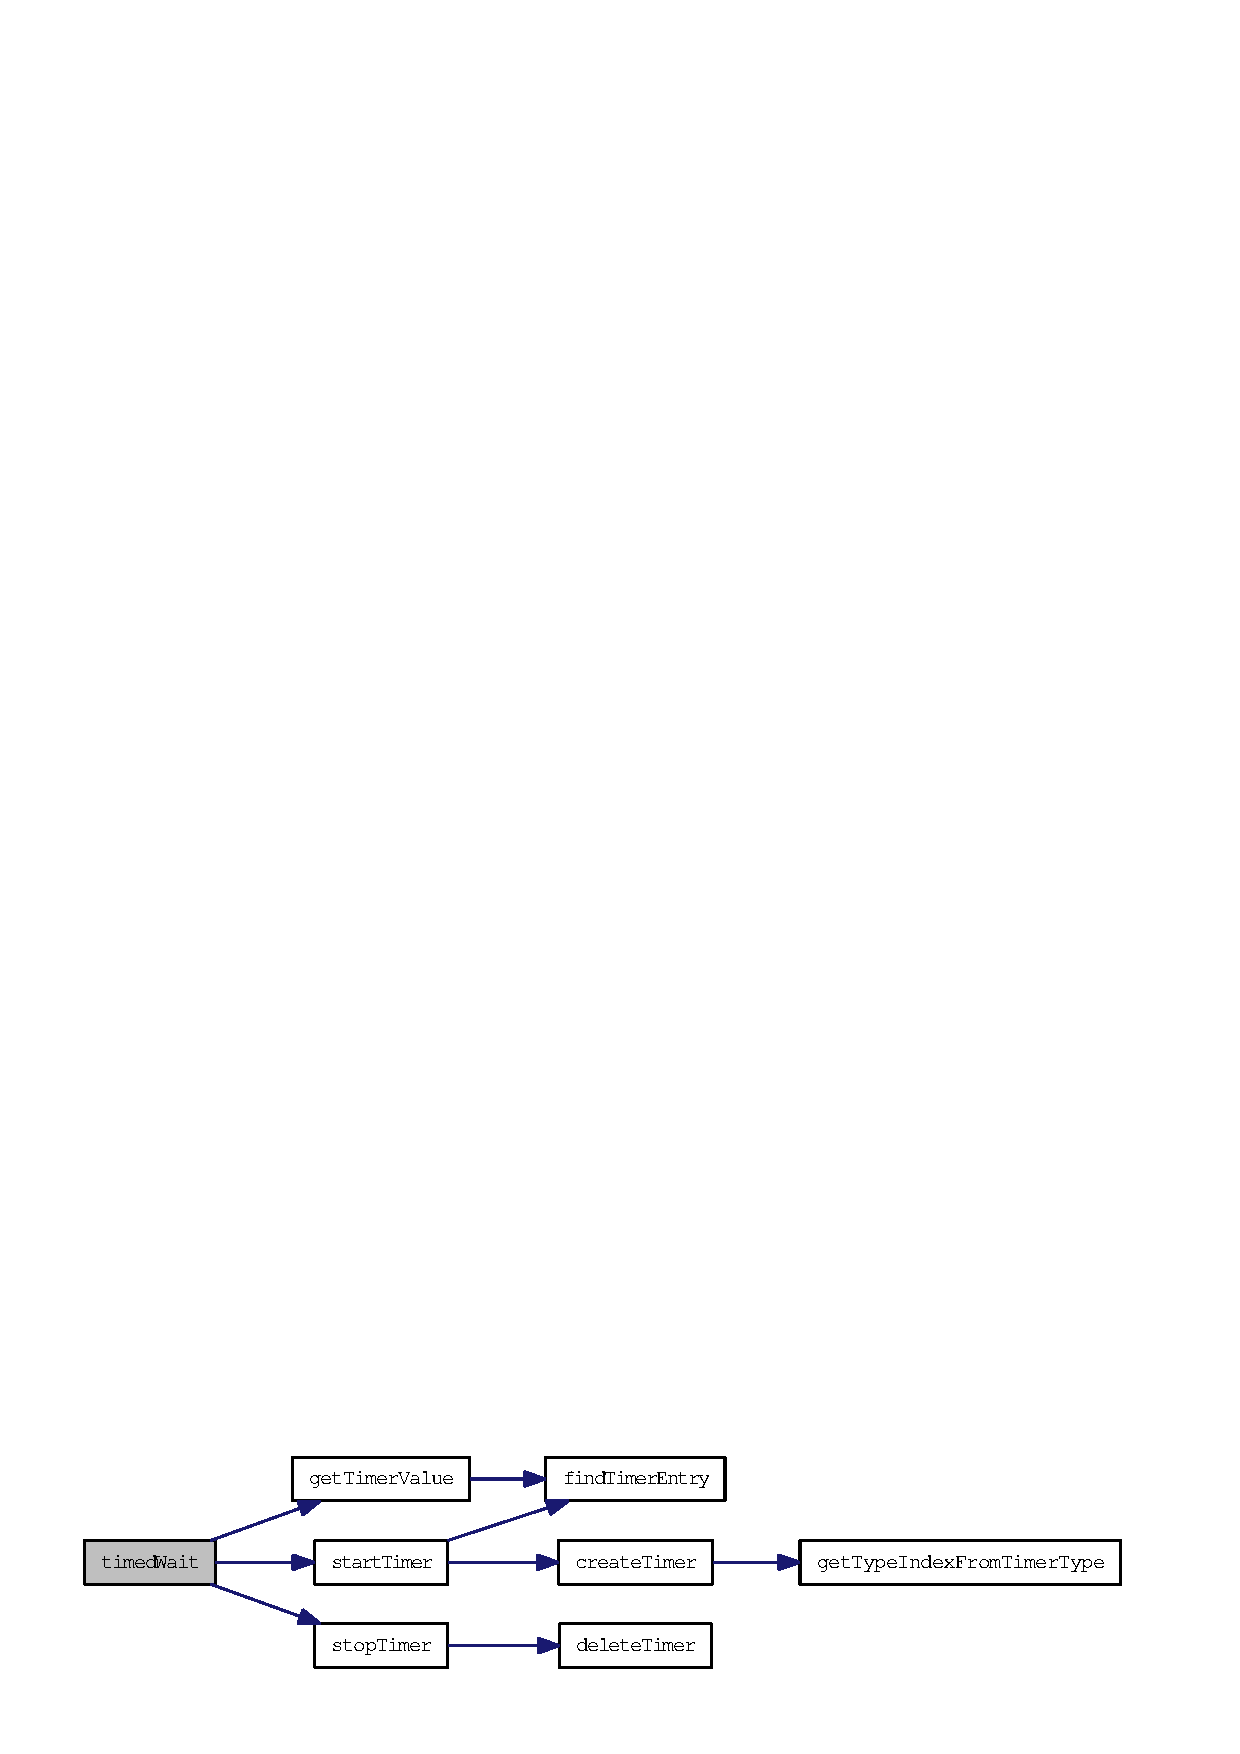
\includegraphics[width=271pt]{cmdInterpreter_8c_ac7fb947e83d5813fb30995133f29955_cgraph}
\end{center}
\end{figure}
\hypertarget{cmdInterpreter_8c_a78c9a935a342b0b7b9a3c9896c5e85b}{
\index{cmdInterpreter.c@{cmd\-Interpreter.c}!waitCondition@{waitCondition}}
\index{waitCondition@{waitCondition}!cmdInterpreter.c@{cmd\-Interpreter.c}}
\subsubsection[waitCondition]{\setlength{\rightskip}{0pt plus 5cm}int wait\-Condition (const char $\ast$$\ast$ {\em array\-Arg}, int {\em i\-Nof\-Args})}}
\label{cmdInterpreter_8c_a78c9a935a342b0b7b9a3c9896c5e85b}




Definition at line 304 of file cmd\-Interpreter.c.

References DBG\_\-ARGUMENT\_\-CONVERT, DBG\_\-CHECK\_\-COMMAND, e\_\-continue, e\_\-fail, get\-Hex\-Number\-From\-Arg(), get\-Timer\-Value(), rcu\-Single\-Read(), read\-Time(), set\-Debug\-Option\-Flag(), start\-Simulation(), start\-Timer(), stop\-Simulation(), stop\-Timer(), and TCondition::type.

Referenced by execute\-Main\-Commands().

Here is the call graph for this function:\begin{figure}[H]
\begin{center}
\leavevmode
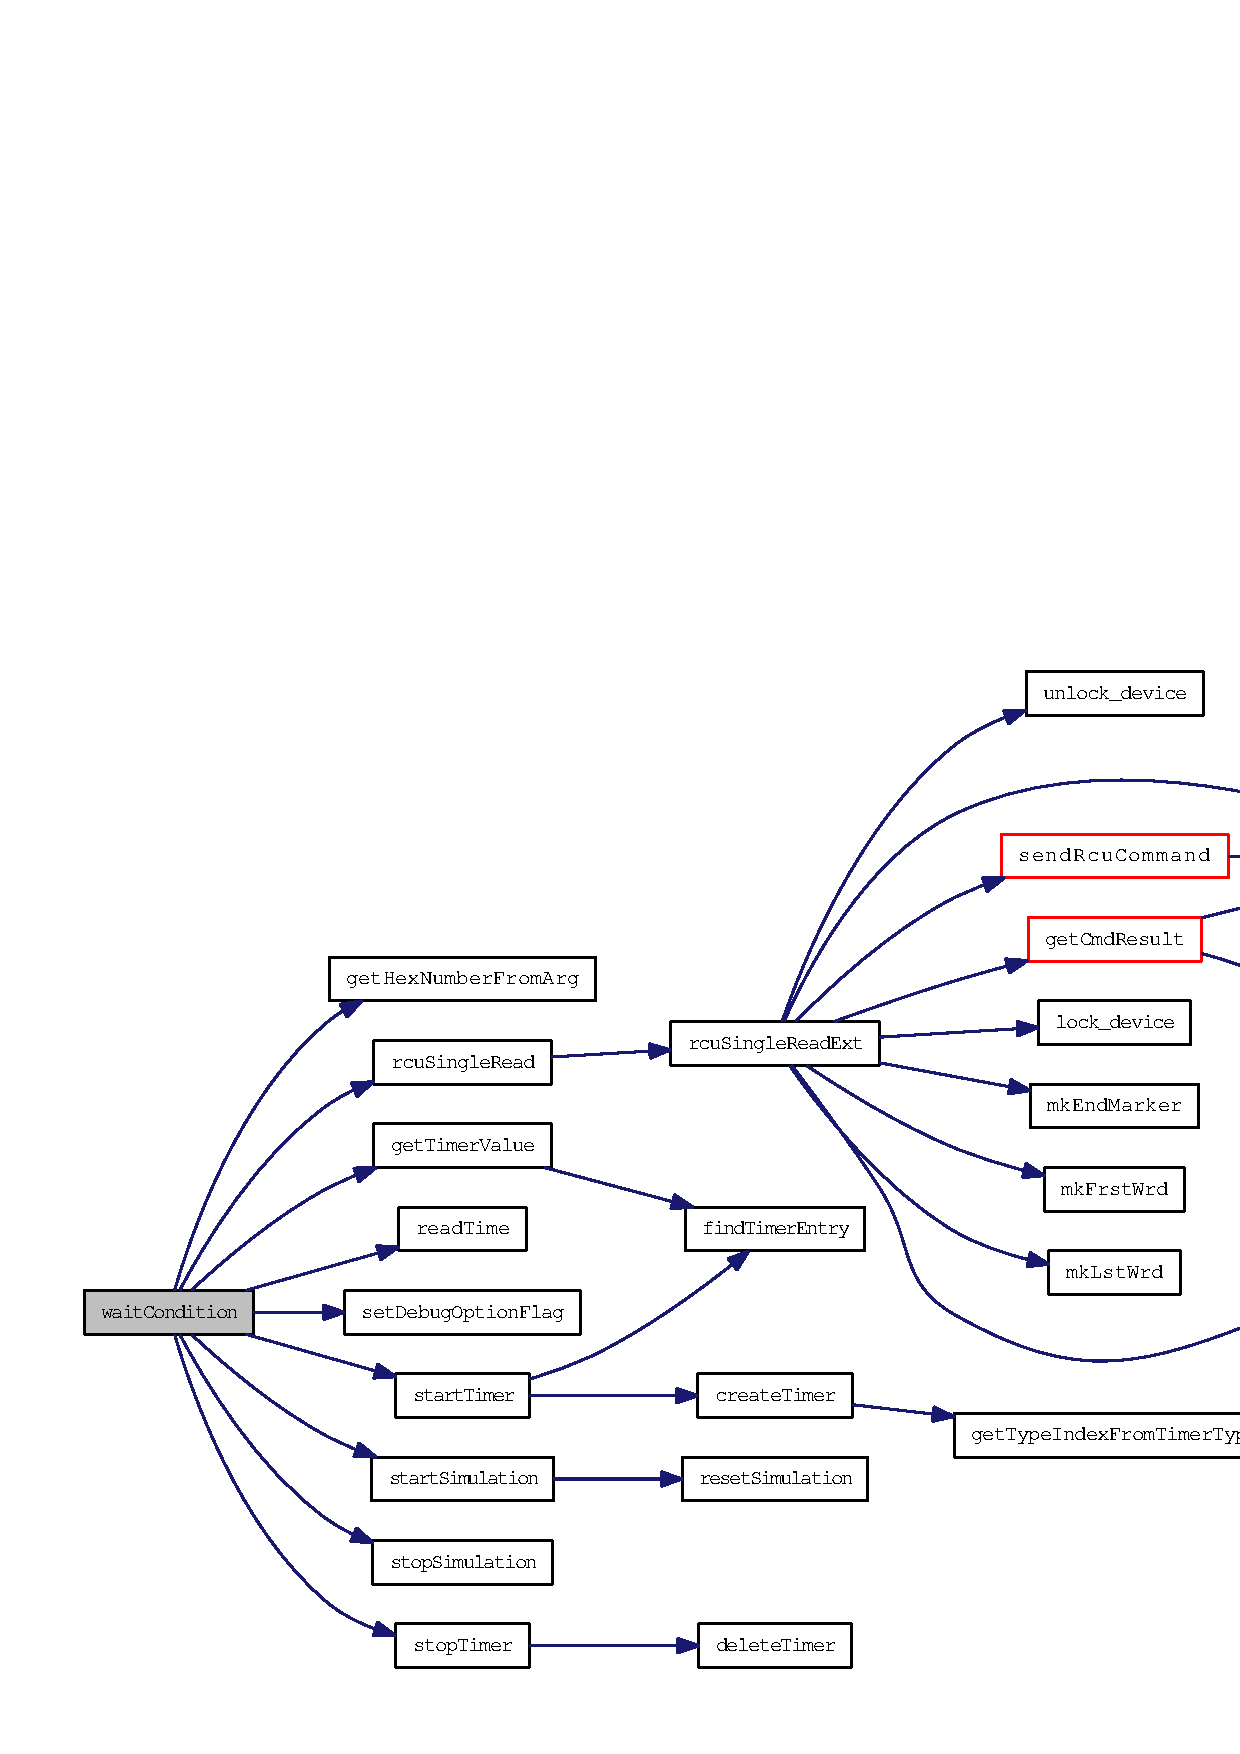
\includegraphics[width=374pt]{cmdInterpreter_8c_a78c9a935a342b0b7b9a3c9896c5e85b_cgraph}
\end{center}
\end{figure}


\subsection{Variable Documentation}
\hypertarget{cmdInterpreter_8c_c1784239c15c2f1b5b4f1dbda9df65e7}{
\index{cmdInterpreter.c@{cmd\-Interpreter.c}!ctrlRegCmds@{ctrlRegCmds}}
\index{ctrlRegCmds@{ctrlRegCmds}!cmdInterpreter.c@{cmd\-Interpreter.c}}
\subsubsection[ctrlRegCmds]{\setlength{\rightskip}{0pt plus 5cm}\hyperlink{structArgDef__t}{TArg\-Def} \hyperlink{cmdInterpreter_8c_c1784239c15c2f1b5b4f1dbda9df65e7}{ctrl\-Reg\-Cmds}\mbox{[}$\,$\mbox{]}}}
\label{cmdInterpreter_8c_c1784239c15c2f1b5b4f1dbda9df65e7}


\textbf{Initial value:}

\begin{Code}\begin{verbatim} {
  {"","",{eUnknownType, {NULL}},{NULL},ARGDEF_TERMINATE},
}
\end{verbatim}\end{Code}


Definition at line 1876 of file cmd\-Interpreter.c.\hypertarget{cmdInterpreter_8c_083a182722ef62f10a68012ab6d7f707}{
\index{cmdInterpreter.c@{cmd\-Interpreter.c}!driverCtrlArgs@{driverCtrlArgs}}
\index{driverCtrlArgs@{driverCtrlArgs}!cmdInterpreter.c@{cmd\-Interpreter.c}}
\subsubsection[driverCtrlArgs]{\setlength{\rightskip}{0pt plus 5cm}\hyperlink{structArgDef__t}{TArg\-Def} \hyperlink{cmdInterpreter_8c_083a182722ef62f10a68012ab6d7f707}{driver\-Ctrl\-Args}\mbox{[}$\,$\mbox{]}}}
\label{cmdInterpreter_8c_083a182722ef62f10a68012ab6d7f707}


\textbf{Initial value:}

\begin{Code}\begin{verbatim} {
  {"i","info",{eFctIndex, {(void*)printDriverInfo}},{(void*)1},ARGDEF_BREAK},
  {"l","lock",{eFctIndex, {(void*)dcscLockCtrl}},{(void*)eLock},ARGDEF_BREAK},
  {"u","unlock",{eFctIndex, {(void*)dcscLockCtrl}},{(void*)eUnlock},ARGDEF_BREAK},
  {"r","reset",{eFctIndex, {(void*)dcscLockCtrl}},{(void*)eDeactivateLock},ARGDEF_BREAK},
  {"a","activate",{eFctIndex, {(void*)dcscLockCtrl}},{(void*)eActivateLock},ARGDEF_BREAK},
  {NULL,"seize",{eFctIndex, {(void*)dcscLockCtrl}},{(void*)eSeize},ARGDEF_BREAK},
  {NULL,"release",{eFctIndex, {(void*)dcscLockCtrl}},{(void*)eRelease},ARGDEF_BREAK},
  {NULL,"debug",{eHex, {NULL}},{NULL},ARGDEF_BREAK},
  {"","",{eUnknownType, {NULL}},{NULL},ARGDEF_TERMINATE},
}
\end{verbatim}\end{Code}


Definition at line 1427 of file cmd\-Interpreter.c.\hypertarget{cmdInterpreter_8c_3e75245c450c10d2323442d359f053d7}{
\index{cmdInterpreter.c@{cmd\-Interpreter.c}!driverCtrlDesc@{driverCtrlDesc}}
\index{driverCtrlDesc@{driverCtrlDesc}!cmdInterpreter.c@{cmd\-Interpreter.c}}
\subsubsection[driverCtrlDesc]{\setlength{\rightskip}{0pt plus 5cm}\hyperlink{structFctArg__t}{TFct\-Arg} \hyperlink{cmdInterpreter_8c_3e75245c450c10d2323442d359f053d7}{driver\-Ctrl\-Desc}}}
\label{cmdInterpreter_8c_3e75245c450c10d2323442d359f053d7}


\textbf{Initial value:}

\begin{Code}\begin{verbatim} {
  driverCtrlArgs,
  NULL,
  NULL
}
\end{verbatim}\end{Code}


Definition at line 1439 of file cmd\-Interpreter.c.\hypertarget{cmdInterpreter_8c_5a94aee581a390576806909f67968c30}{
\index{cmdInterpreter.c@{cmd\-Interpreter.c}!firmwareCmds@{firmwareCmds}}
\index{firmwareCmds@{firmwareCmds}!cmdInterpreter.c@{cmd\-Interpreter.c}}
\subsubsection[firmwareCmds]{\setlength{\rightskip}{0pt plus 5cm}\hyperlink{structArgDef__t}{TArg\-Def} \hyperlink{cmdInterpreter_8c_5a94aee581a390576806909f67968c30}{firmware\-Cmds}\mbox{[}$\,$\mbox{]}}}
\label{cmdInterpreter_8c_5a94aee581a390576806909f67968c30}


\textbf{Initial value:}

\begin{Code}\begin{verbatim} {
  {"r","reset",{eFctIndex, {(void*)rcuBusControlCmd}},{(void*)eResetFirmware},ARGDEF_TERMINATE},
  {"wr","write-reg",{eFctUserScan, {(void*)execRegWriteCmd}},{NULL},ARGDEF_TERMINATE},
  {"rr","read-reg", {eFctUserScan, {(void*)execRegReadCmd}}, {NULL},ARGDEF_TERMINATE},
  {"ec","enable-comp",{eFctIndex, {(void*)rcuBusControlCmd}},{(void*)eEnableCompression},ARGDEF_TERMINATE},
  {"dc","enable-comp",{eFctIndex, {(void*)rcuBusControlCmd}},{(void*)eDisableCompression},ARGDEF_TERMINATE},
  {"*",NULL,{eFctNoArg, {(void*)printFirmwareHelp}},{NULL},ARGDEF_TERMINATE},
  {"","",{eUnknownType, {NULL}},{NULL},ARGDEF_TERMINATE},
}
\end{verbatim}\end{Code}


Definition at line 1866 of file cmd\-Interpreter.c.\hypertarget{cmdInterpreter_8c_5a3ddbaacf0c338e408e3c0b55189d58}{
\index{cmdInterpreter.c@{cmd\-Interpreter.c}!flashCmds@{flashCmds}}
\index{flashCmds@{flashCmds}!cmdInterpreter.c@{cmd\-Interpreter.c}}
\subsubsection[flashCmds]{\setlength{\rightskip}{0pt plus 5cm}\hyperlink{structArgDef__t}{TArg\-Def} \hyperlink{cmdInterpreter_8c_5a3ddbaacf0c338e408e3c0b55189d58}{flash\-Cmds}\mbox{[}$\,$\mbox{]}}}
\label{cmdInterpreter_8c_5a3ddbaacf0c338e408e3c0b55189d58}


\textbf{Initial value:}

\begin{Code}\begin{verbatim} {
  {"e","enable",{eFctIndex, {(void*)rcuBusControlCmd}},{(void*)eEnableFlash},ARGDEF_TERMINATE},
  {"d","disable",{eFctIndex, {(void*)rcuBusControlCmd}},{(void*)eDisableFlash},ARGDEF_TERMINATE},
  {NULL,"reset",{eFctIndex, {(void*)rcuBusControlCmd}},{(void*)eResetFlash},ARGDEF_TERMINATE},
  {NULL,"id",{eFctIndex, {(void*)rcuBusControlCmd}},{(void*)eFlashID},ARGDEF_TERMINATE},
  {NULL,"ctrldcs",{eFctIndex, {(void*)rcuBusControlCmd}},{(void*)eFlashCtrlDCS},ARGDEF_TERMINATE},
  {NULL,"ctrlactel",{eFctIndex, {(void*)rcuBusControlCmd}},{(void*)eFlashCtrlActel},ARGDEF_TERMINATE},
  {"w","write",{eFctUserScan, {(void*)execFlashWriteCmd}},{NULL},ARGDEF_TERMINATE},
  {"r","read",{eFctUserScan, {(void*)execFlashReadCmd}},{NULL},ARGDEF_TERMINATE},
  {"v","verify",{eFctUserScan, {(void*)execFlashVerifyCmd}},{NULL},ARGDEF_TERMINATE},
  {NULL,"erase",{eFctArgDef, {(void*)execFlashErase}},{(void*)&flashEraseDesc},ARGDEF_TERMINATE},
  {NULL,"eraseall",{eFctNoArg, {(void*)execFlashEraseall}},{NULL},ARGDEF_TERMINATE},
  {"*",NULL,{eFctNoArg, {(void*)printFlashHelp}},{NULL},ARGDEF_TERMINATE},
  {"","",{eUnknownType, {NULL}},{NULL},ARGDEF_TERMINATE},
}
\end{verbatim}\end{Code}


Definition at line 1850 of file cmd\-Interpreter.c.\hypertarget{cmdInterpreter_8c_9a757fd68a4d59000e0938fcdb423996}{
\index{cmdInterpreter.c@{cmd\-Interpreter.c}!flashEraseDesc@{flashEraseDesc}}
\index{flashEraseDesc@{flashEraseDesc}!cmdInterpreter.c@{cmd\-Interpreter.c}}
\subsubsection[flashEraseDesc]{\setlength{\rightskip}{0pt plus 5cm}\hyperlink{structFctArg__t}{TFct\-Arg} \hyperlink{cmdInterpreter_8c_9a757fd68a4d59000e0938fcdb423996}{flash\-Erase\-Desc}}}
\label{cmdInterpreter_8c_9a757fd68a4d59000e0938fcdb423996}


\textbf{Initial value:}

\begin{Code}\begin{verbatim} {
  flashEraseParams,
  NULL,
  NULL
}
\end{verbatim}\end{Code}


Definition at line 1844 of file cmd\-Interpreter.c.\hypertarget{cmdInterpreter_8c_7399e2dab99f698c9275622762e94f74}{
\index{cmdInterpreter.c@{cmd\-Interpreter.c}!flashEraseParams@{flashEraseParams}}
\index{flashEraseParams@{flashEraseParams}!cmdInterpreter.c@{cmd\-Interpreter.c}}
\subsubsection[flashEraseParams]{\setlength{\rightskip}{0pt plus 5cm}\hyperlink{structArgDef__t}{TArg\-Def} \hyperlink{cmdInterpreter_8c_7399e2dab99f698c9275622762e94f74}{flash\-Erase\-Params}\mbox{[}$\,$\mbox{]}}}
\label{cmdInterpreter_8c_7399e2dab99f698c9275622762e94f74}


\textbf{Initial value:}

\begin{Code}\begin{verbatim} {
  {NULL,"all",{eBool, {(void*)0}},{(void*)NULL},ARGDEF_BREAK},
  {"sec","sector",{eHex, {(void*)0}},{(void*)NULL},0},
  {NULL,"_count",{eInteger, {(void*)0}},{(void*)NULL},ARGDEF_RESUME|ARGDEF_KEYWORDLESS},
  {"","",{eUnknownType, {NULL}},{NULL},ARGDEF_TERMINATE},
}
\end{verbatim}\end{Code}


Definition at line 1837 of file cmd\-Interpreter.c.\hypertarget{cmdInterpreter_8c_0aee2ec97f7e88992f9b2b333ca99be2}{
\index{cmdInterpreter.c@{cmd\-Interpreter.c}!g_bBatchProcessing@{g\_\-bBatchProcessing}}
\index{g_bBatchProcessing@{g\_\-bBatchProcessing}!cmdInterpreter.c@{cmd\-Interpreter.c}}
\subsubsection[g\_\-bBatchProcessing]{\setlength{\rightskip}{0pt plus 5cm}int \hyperlink{cmdInterpreter_8c_0aee2ec97f7e88992f9b2b333ca99be2}{g\_\-b\-Batch\-Processing} = 0}}
\label{cmdInterpreter_8c_0aee2ec97f7e88992f9b2b333ca99be2}




Definition at line 1279 of file cmd\-Interpreter.c.

Referenced by exec\-Batch(), and terminate\-Batch\-Processing().\hypertarget{cmdInterpreter_8c_b1b44b602185677d4a2a372121627437}{
\index{cmdInterpreter.c@{cmd\-Interpreter.c}!g_profiling@{g\_\-profiling}}
\index{g_profiling@{g\_\-profiling}!cmdInterpreter.c@{cmd\-Interpreter.c}}
\subsubsection[g\_\-profiling]{\setlength{\rightskip}{0pt plus 5cm}int \hyperlink{cmdInterpreter_8c_b1b44b602185677d4a2a372121627437}{g\_\-profiling} = 0}}
\label{cmdInterpreter_8c_b1b44b602185677d4a2a372121627437}




Definition at line 60 of file cmd\-Interpreter.c.

Referenced by exec\-Batch(), execute\-Main\-Commands(), and exec\-Write\-Cmd().\hypertarget{cmdInterpreter_8c_014d78494c13d4dc0430ee68de158559}{
\index{cmdInterpreter.c@{cmd\-Interpreter.c}!mainCommands@{mainCommands}}
\index{mainCommands@{mainCommands}!cmdInterpreter.c@{cmd\-Interpreter.c}}
\subsubsection[mainCommands]{\setlength{\rightskip}{0pt plus 5cm}\hyperlink{structArgDef__t}{TArg\-Def} \hyperlink{cmdInterpreter_8c_014d78494c13d4dc0430ee68de158559}{main\-Commands}\mbox{[}$\,$\mbox{]}}}
\label{cmdInterpreter_8c_014d78494c13d4dc0430ee68de158559}


\textbf{Initial value:}

\begin{Code}\begin{verbatim} {
  {"sm","selectmap",{eFctRemaining, {(void*)selectmapCmds}},{(void*)&scanModeDefault},ARGDEF_TERMINATE},
  {NULL,"flash",{eFctRemaining, {(void*)flashCmds}},{(void*)&scanModeDefault},ARGDEF_TERMINATE},
  {"fw","firmware",{eFctRemaining, {(void*)firmwareCmds}},{(void*)&scanModeDefault},ARGDEF_TERMINATE},
  {"rcr","read-ctrlreg",{eFctNoArg, {(void*)ctrlRegStatus}},{NULL},ARGDEF_TERMINATE},
  {"d","driver",{eFctArgDef, {(void*)driverCtrlCmds}},{(void*)&driverCtrlDesc},ARGDEF_TERMINATE},
  {"i","info",{eFctNoArg, {(void*)printInfo}},{NULL},ARGDEF_TERMINATE},
  {"#",NULL,{eBool, {NULL}},{NULL},ARGDEF_TERMINATE},
  {NULL,"*",{eFctUserScan, {(void*)executeMainCommands}},{NULL},ARGDEF_TERMINATE},
  {"","",{eUnknownType, {NULL}},{NULL},ARGDEF_TERMINATE},
}
\end{verbatim}\end{Code}


Definition at line 1880 of file cmd\-Interpreter.c.

Referenced by execute\-Command\-Args().\hypertarget{cmdInterpreter_8c_fbc09bb85c6e4618a38dba855c588abd}{
\index{cmdInterpreter.c@{cmd\-Interpreter.c}!scanModeDefault@{scanModeDefault}}
\index{scanModeDefault@{scanModeDefault}!cmdInterpreter.c@{cmd\-Interpreter.c}}
\subsubsection[scanModeDefault]{\setlength{\rightskip}{0pt plus 5cm}\hyperlink{structFctMode__t}{TFct\-Mode} \hyperlink{cmdInterpreter_8c_fbc09bb85c6e4618a38dba855c588abd}{scan\-Mode\-Default} = \{SCANMODE\_\-FORCE\_\-TERMINATION, NULL, NULL\}}}
\label{cmdInterpreter_8c_fbc09bb85c6e4618a38dba855c588abd}




Definition at line 1826 of file cmd\-Interpreter.c.\hypertarget{cmdInterpreter_8c_4954a4ac4d6f82836d8b405a2ec86071}{
\index{cmdInterpreter.c@{cmd\-Interpreter.c}!selectmapCmds@{selectmapCmds}}
\index{selectmapCmds@{selectmapCmds}!cmdInterpreter.c@{cmd\-Interpreter.c}}
\subsubsection[selectmapCmds]{\setlength{\rightskip}{0pt plus 5cm}\hyperlink{structArgDef__t}{TArg\-Def} \hyperlink{cmdInterpreter_8c_4954a4ac4d6f82836d8b405a2ec86071}{selectmap\-Cmds}\mbox{[}$\,$\mbox{]}}}
\label{cmdInterpreter_8c_4954a4ac4d6f82836d8b405a2ec86071}


\textbf{Initial value:}

\begin{Code}\begin{verbatim} {
  {"e","enable",{eFctIndex, {(void*)rcuBusControlCmd}},{(void*)eEnableSelectmap},ARGDEF_TERMINATE},
  {"d","disable",{eFctIndex, {(void*)rcuBusControlCmd}},{(void*)eDisableSelectmap},ARGDEF_TERMINATE},
  {"wr","write-reg",{eFctUserScan, {(void*)execSmWriteReg}},{NULL},ARGDEF_TERMINATE},
  {"rr","read-reg",{eFctUserScan, {(void*)execSmReadReg}},{NULL},ARGDEF_TERMINATE},
  {"*",NULL,{eFctNoArg, {(void*)printSelectmapHelp}},{NULL},ARGDEF_TERMINATE},
  {"","",{eUnknownType, {NULL}},{NULL},ARGDEF_TERMINATE},
}
\end{verbatim}\end{Code}


Definition at line 1828 of file cmd\-Interpreter.c.
\hypertarget{cmdInterpreter_8h}{
\section{cmd\-Interpreter.h File Reference}
\label{cmdInterpreter_8h}\index{cmdInterpreter.h@{cmdInterpreter.h}}
}


This graph shows which files directly or indirectly include this file:\begin{figure}[H]
\begin{center}
\leavevmode
\includegraphics[width=147pt]{cmdInterpreter_8h__dep__incl}
\end{center}
\end{figure}
\subsection*{Defines}
\begin{CompactItemize}
\item 
\#define \hyperlink{cmdInterpreter_8h_c998ea02fbd821fc123d60445ce76f38}{UINT\_\-MAX}~0xffffffff
\item 
\#define \hyperlink{cmdInterpreter_8h_c4d12945dc541519caef4f461062a6c5}{INT\_\-RO\_\-MAX}~0xffff
\end{CompactItemize}
\subsection*{Functions}
\begin{CompactItemize}
\item 
int \hyperlink{cmdInterpreter_8h_54cbd6e4f4a91310f0c408dc5c6b413d}{execute\-Command\-Args} (int i\-Nof\-Args, const char $\ast$$\ast$array\-Arg)
\item 
int \hyperlink{cmdInterpreter_8h_48086998882e7d163126de4100aa12ac}{execute\-Command\-Line} (char $\ast$p\-Cmd\-Line)
\item 
int \hyperlink{cmdInterpreter_8h_ae37490e691f5b4d2c2e8f22713555da}{terminate\-Batch\-Processing} ()
\item 
int \hyperlink{cmdInterpreter_8h_f03f7609a66def2e7fae02a477c38d97}{print\-Help} ()
\item 
int \hyperlink{cmdInterpreter_8h_ac3ae2fb745e63e33060d5c0b658f745}{print\-Info} ()
\end{CompactItemize}


\subsection{Define Documentation}
\hypertarget{cmdInterpreter_8h_c4d12945dc541519caef4f461062a6c5}{
\index{cmdInterpreter.h@{cmd\-Interpreter.h}!INT_RO_MAX@{INT\_\-RO\_\-MAX}}
\index{INT_RO_MAX@{INT\_\-RO\_\-MAX}!cmdInterpreter.h@{cmd\-Interpreter.h}}
\subsubsection[INT\_\-RO\_\-MAX]{\setlength{\rightskip}{0pt plus 5cm}\#define INT\_\-RO\_\-MAX~0xffff}}
\label{cmdInterpreter_8h_c4d12945dc541519caef4f461062a6c5}




Definition at line 33 of file cmd\-Interpreter.h.

Referenced by print\-Read\-Output\-Formatted().\hypertarget{cmdInterpreter_8h_c998ea02fbd821fc123d60445ce76f38}{
\index{cmdInterpreter.h@{cmd\-Interpreter.h}!UINT_MAX@{UINT\_\-MAX}}
\index{UINT_MAX@{UINT\_\-MAX}!cmdInterpreter.h@{cmd\-Interpreter.h}}
\subsubsection[UINT\_\-MAX]{\setlength{\rightskip}{0pt plus 5cm}\#define UINT\_\-MAX~0xffffffff}}
\label{cmdInterpreter_8h_c998ea02fbd821fc123d60445ce76f38}




Definition at line 25 of file cmd\-Interpreter.h.

Referenced by print\-Read\-Output\-Formatted().

\subsection{Function Documentation}
\hypertarget{cmdInterpreter_8h_54cbd6e4f4a91310f0c408dc5c6b413d}{
\index{cmdInterpreter.h@{cmd\-Interpreter.h}!executeCommandArgs@{executeCommandArgs}}
\index{executeCommandArgs@{executeCommandArgs}!cmdInterpreter.h@{cmd\-Interpreter.h}}
\subsubsection[executeCommandArgs]{\setlength{\rightskip}{0pt plus 5cm}int execute\-Command\-Args (int {\em i\-Nof\-Args}, const char $\ast$$\ast$ {\em array\-Arg})}}
\label{cmdInterpreter_8h_54cbd6e4f4a91310f0c408dc5c6b413d}




Definition at line 1892 of file cmd\-Interpreter.c.

References main\-Commands, mr\-Shell\-Prim\-Clone\-Def(), and Scan\-Arguments().

Referenced by execute\-Command\-Line(), and main().

Here is the call graph for this function:\begin{figure}[H]
\begin{center}
\leavevmode
\includegraphics[width=313pt]{cmdInterpreter_8h_54cbd6e4f4a91310f0c408dc5c6b413d_cgraph}
\end{center}
\end{figure}
\hypertarget{cmdInterpreter_8h_48086998882e7d163126de4100aa12ac}{
\index{cmdInterpreter.h@{cmd\-Interpreter.h}!executeCommandLine@{executeCommandLine}}
\index{executeCommandLine@{executeCommandLine}!cmdInterpreter.h@{cmd\-Interpreter.h}}
\subsubsection[executeCommandLine]{\setlength{\rightskip}{0pt plus 5cm}int execute\-Command\-Line (char $\ast$ {\em p\-Cmd\-Line})}}
\label{cmdInterpreter_8h_48086998882e7d163126de4100aa12ac}




Definition at line 1904 of file cmd\-Interpreter.c.

References build\-Arguments\-From\-Command\-Line(), DBG\_\-ARGUMENT\_\-CONVERT, execute\-Command\-Args(), and set\-Debug\-Option\-Flag().

Referenced by exec\-Batch(), and main().

Here is the call graph for this function:\begin{figure}[H]
\begin{center}
\leavevmode
\includegraphics[width=273pt]{cmdInterpreter_8h_48086998882e7d163126de4100aa12ac_cgraph}
\end{center}
\end{figure}
\hypertarget{cmdInterpreter_8h_f03f7609a66def2e7fae02a477c38d97}{
\index{cmdInterpreter.h@{cmd\-Interpreter.h}!printHelp@{printHelp}}
\index{printHelp@{printHelp}!cmdInterpreter.h@{cmd\-Interpreter.h}}
\subsubsection[printHelp]{\setlength{\rightskip}{0pt plus 5cm}int print\-Help ()}}
\label{cmdInterpreter_8h_f03f7609a66def2e7fae02a477c38d97}




Definition at line 198 of file cmd\-Interpreter.c.

Referenced by execute\-Main\-Commands().\hypertarget{cmdInterpreter_8h_ac3ae2fb745e63e33060d5c0b658f745}{
\index{cmdInterpreter.h@{cmd\-Interpreter.h}!printInfo@{printInfo}}
\index{printInfo@{printInfo}!cmdInterpreter.h@{cmd\-Interpreter.h}}
\subsubsection[printInfo]{\setlength{\rightskip}{0pt plus 5cm}int print\-Info ()}}
\label{cmdInterpreter_8h_ac3ae2fb745e63e33060d5c0b658f745}




Definition at line 164 of file cmd\-Interpreter.c.\hypertarget{cmdInterpreter_8h_ae37490e691f5b4d2c2e8f22713555da}{
\index{cmdInterpreter.h@{cmd\-Interpreter.h}!terminateBatchProcessing@{terminateBatchProcessing}}
\index{terminateBatchProcessing@{terminateBatchProcessing}!cmdInterpreter.h@{cmd\-Interpreter.h}}
\subsubsection[terminateBatchProcessing]{\setlength{\rightskip}{0pt plus 5cm}int terminate\-Batch\-Processing ()}}
\label{cmdInterpreter_8h_ae37490e691f5b4d2c2e8f22713555da}




Definition at line 1280 of file cmd\-Interpreter.c.

References g\_\-b\-Batch\-Processing.

Referenced by sigquit\-Handler().
\hypertarget{backup_2dcs__driver_8c}{
\section{dcs\_\-driver.c File Reference}
\label{backup_2dcs__driver_8c}\index{dcs_driver.c@{dcs\_\-driver.c}}
}
{\tt \#include $<$linux/fs.h$>$}\par
{\tt \#include $<$linux/types.h$>$}\par
{\tt \#include $<$linux/sched.h$>$}\par
{\tt \#include $<$linux/errno.h$>$}\par
{\tt \#include $<$linux/slab.h$>$}\par
{\tt \#include $<$asm/io.h$>$}\par
{\tt \#include $<$asm/uaccess.h$>$}\par
{\tt \#include $<$linux/mm.h$>$}\par
{\tt \#include $<$linux/ioport.h$>$}\par
{\tt \#include $<$linux/spinlock.h$>$}\par
{\tt \#include $<$asm/system.h$>$}\par
{\tt \#include $<$linux/module.h$>$}\par
{\tt \#include \char`\"{}dcs\_\-driver.h\char`\"{}}\par
{\tt \#include \char`\"{}version.h\char`\"{}}\par
{\tt \#include \char`\"{}mr\-Kern\-Logging.c\char`\"{}}\par


Include dependency graph for backup/dcs\_\-driver.c:\begin{figure}[H]
\begin{center}
\leavevmode
\includegraphics[width=193pt]{backup_2dcs__driver_8c__incl}
\end{center}
\end{figure}
\subsection*{Defines}
\begin{CompactItemize}
\item 
\#define \hyperlink{backup_2dcs__driver_8c_805e10412728f32d8585dd436b22cc99}{TEST\_\-PATTERN}~0x13071972
\end{CompactItemize}
\subsection*{Functions}
\begin{CompactItemize}
\item 
\hyperlink{backup_2dcs__driver_8c_3053a7067223a09a392be7f5871f9766}{MODULE\_\-PARM} (\hyperlink{dcs__driver_8c_45c631d40e14d14a309abbe2b87ccd1b}{dcsc\_\-major\-ID},\char`\"{}i\char`\"{})
\item 
\hyperlink{backup_2dcs__driver_8c_75f25d27ddf2830f44e578fb39146b97}{MODULE\_\-PARM} (\hyperlink{dcs__driver_8c_9a8b5688625d4564010909cb4e23192f}{dcsc\_\-msgbuf\_\-in\_\-size},\char`\"{}i\char`\"{})
\item 
\hyperlink{backup_2dcs__driver_8c_d2a9008a63b5fc661f4aa83a8a0f8bcc}{MODULE\_\-PARM} (\hyperlink{dcs__driver_8c_57243357aaca143dc0a0e93dcd16eb89}{dcsc\_\-msgbuf\_\-out\_\-size},\char`\"{}i\char`\"{})
\item 
\hyperlink{backup_2dcs__driver_8c_19e37b390f71b35e88960d78c6d836c4}{MODULE\_\-PARM} (\hyperlink{dcs__driver_8c_898ab396bb466832c0c38ecc37f16632}{dcsc\_\-regfile\_\-size},\char`\"{}i\char`\"{})
\item 
\hyperlink{backup_2dcs__driver_8c_73936caf0f944aa65a75a16e077c835a}{MODULE\_\-PARM} (\hyperlink{dcs__driver_8c_03af36d4209f6364a9f7a5f1087f19f9}{msgbuf\_\-in\_\-physaddr},\char`\"{}i\char`\"{})
\item 
\hyperlink{backup_2dcs__driver_8c_b8f38a668f504ecdbf2041c14fc8f50f}{MODULE\_\-PARM} (\hyperlink{dcs__driver_8c_89c68fc835da1b91e1d93eecb77922b6}{msgbuf\_\-out\_\-physaddr},\char`\"{}i\char`\"{})
\item 
\hyperlink{backup_2dcs__driver_8c_84a8ddb935ced6da7bdd97965f36cead}{MODULE\_\-PARM} (\hyperlink{dcs__driver_8c_607a6fb1f19bf1e11ec4fa99dc7efecd}{regfile\_\-physaddr},\char`\"{}i\char`\"{})
\item 
\hyperlink{backup_2dcs__driver_8c_53fff30413e173391c35bdc5481c1719}{MODULE\_\-AUTHOR} (\char`\"{}Matthias Richter\char`\"{})
\item 
\hyperlink{backup_2dcs__driver_8c_2eb38dffd9d03b7908c57b56ae9e9377}{MODULE\_\-DESCRIPTION} (\char`\"{}dcs-card register driver\char`\"{})
\item 
\hyperlink{backup_2dcs__driver_8c_d94b36675e7eb067ea3ce6ff9e244a44}{MODULE\_\-LICENSE} (\char`\"{}GPL\char`\"{})
\item 
static int \hyperlink{backup_2dcs__driver_8c_5fc9e61f41c571cca4373a64ca28d159}{memtest} (u32 begin, u32 size)
\item 
static int \hyperlink{backup_2dcs__driver_8c_24611c859ab5512627f0ebe5e71bb7df}{dcs\_\-comparevalue} (u32 begin, u32 size, u32 value)
\item 
static int \hyperlink{backup_2dcs__driver_8c_aec6947dd189feeedeb22af3fbc21d81}{dcs\_\-writevalue} (u32 begin, u32 size, u32 value)
\item 
static int \hyperlink{backup_2dcs__driver_8c_85874c4901b4b811c882944a3f77ff0e}{dcs\_\-read} (u32 begin, u32 size, u32 $\ast$buff)
\item 
static int \hyperlink{backup_2dcs__driver_8c_626a935595dad9fb4ce5cfdf4fd48f28}{dcs\_\-write} (u32 begin, u32 size, u32 $\ast$buff)
\item 
u32 \hyperlink{backup_2dcs__driver_8c_0f2edb55399fbd36008bbded20c5ecab}{find\-Buffer\-For\-Address} (loff\_\-t offset, int \hyperlink{dcs__driver_8c_269775bb092dfa3a11844c3d1883d988}{i\-Access\-Mode}, u32 $\ast$$\ast$pp\-Buffer, u32 $\ast$p\-Position, const char $\ast$$\ast$pp\-Buffer\-Name)
\item 
int \hyperlink{backup_2dcs__driver_8c_c619293d4edc146efb03fb6b03f8461f}{Init\-Driver\-Lock} ()
\item 
int \hyperlink{backup_2dcs__driver_8c_a754eaa169b47cb26cf5e997276ebd81}{lock\-Activate} ()
\item 
int \hyperlink{backup_2dcs__driver_8c_bfe7c9dd41295bc3fe20fc96aa3ac39d}{lock\-Reset} ()
\item 
int \hyperlink{backup_2dcs__driver_8c_4a2481d7c54d6ec0d99bc8716a8a021f}{check\-And\-Lock} (int i\-Seize\-Code, int pid)
\begin{CompactList}\small\item\em spin-lock protected check of the lock status variable. \item\end{CompactList}\item 
int \hyperlink{backup_2dcs__driver_8c_69f4b1ea76e4eeed7eb2fed3adc6e847}{lock\-Driver} (int i\-Seize\-Code, int i\-Time\-Out)
\begin{CompactList}\small\item\em Try to lock the driver, go to sleep if already locked. \item\end{CompactList}\item 
int \hyperlink{backup_2dcs__driver_8c_f65c837b7c30c1d6c4861e5dbb9a4e59}{seize\-Driver} (int i\-Seize\-Code)
\begin{CompactList}\small\item\em Lock the driver to a single application. \item\end{CompactList}\item 
int \hyperlink{backup_2dcs__driver_8c_0e119609dea51ec090e7852dd9d0abad}{unlock\-Driver} ()
\begin{CompactList}\small\item\em Unlock the driver and wake up all sleeping processes. \item\end{CompactList}\item 
int \hyperlink{backup_2dcs__driver_8c_6ccbabe02e6e0af40d2b653b2a158d40}{release\-Driver} (int i\-Seize\-Code)
\begin{CompactList}\small\item\em Release the driver which was locked to a single application. \item\end{CompactList}\item 
static loff\_\-t \hyperlink{backup_2dcs__driver_8c_1b18195d839987757d645e7761bdfbc1}{dcsc\_\-llseek} (struct file $\ast$filp, loff\_\-t off, int ref)
\item 
static int \hyperlink{backup_2dcs__driver_8c_8067a5efccbb89b363e4b12d4249bb07}{dcsc\_\-read} (struct file $\ast$filp, char $\ast$buf, size\_\-t count, loff\_\-t $\ast$f\_\-pos)
\item 
static int \hyperlink{backup_2dcs__driver_8c_0c28bf0d1a698b2c9c598715bd37a9cb}{dcsc\_\-write} (struct file $\ast$filp, const char $\ast$buf, size\_\-t count, loff\_\-t $\ast$f\_\-pos)
\item 
static int \hyperlink{backup_2dcs__driver_8c_1fc34702f88baf2a47a0434f6ea9e0cb}{dcsc\_\-open} (struct inode $\ast$inode, struct file $\ast$filp)
\item 
static int \hyperlink{backup_2dcs__driver_8c_5350bab3f3d6d1f1e2c84ecafa150d68}{dcsc\_\-close} (struct inode $\ast$inode, struct file $\ast$filp)
\item 
static int \hyperlink{backup_2dcs__driver_8c_c3b4c74273847bef0006306f638cc133}{dcsc\_\-mmap} (struct file $\ast$filp, struct vm\_\-area\_\-struct $\ast$vma)
\item 
static int \hyperlink{backup_2dcs__driver_8c_30d7523911ed6cebd68b1d5c34da9d64}{dcsc\_\-ioctl} (struct inode $\ast$inode, struct file $\ast$filp, unsigned int cmd, unsigned long arg)
\item 
void \hyperlink{backup_2dcs__driver_8c_06a93d1b1348b354639233cdab90e9fe}{cleanup\-Real\-Buffers} ()
\item 
int \hyperlink{backup_2dcs__driver_8c_b3161c882ef5359bf75cf6705c545cd4}{init\-Real\-Buffers} ()
\item 
int \hyperlink{backup_2dcs__driver_8c_e52690ce6969b799366b2c5feba67b8c}{init\_\-module} (void)
\item 
void \hyperlink{backup_2dcs__driver_8c_bb8e1606224e802418862b898888063a}{cleanup\_\-module} (void)
\end{CompactItemize}
\subsection*{Variables}
\begin{CompactItemize}
\item 
int \hyperlink{backup_2dcs__driver_8c_45c631d40e14d14a309abbe2b87ccd1b}{dcsc\_\-major\-ID} = 150
\item 
static int \hyperlink{backup_2dcs__driver_8c_9a8b5688625d4564010909cb4e23192f}{dcsc\_\-msgbuf\_\-in\_\-size} = 0x400
\item 
static int \hyperlink{backup_2dcs__driver_8c_57243357aaca143dc0a0e93dcd16eb89}{dcsc\_\-msgbuf\_\-out\_\-size} = 0x400
\item 
static int \hyperlink{backup_2dcs__driver_8c_898ab396bb466832c0c38ecc37f16632}{dcsc\_\-regfile\_\-size} = 0x10
\item 
static u32 $\ast$ \hyperlink{backup_2dcs__driver_8c_03af36d4209f6364a9f7a5f1087f19f9}{msgbuf\_\-in\_\-physaddr} = ((u32 $\ast$) 0x80000400)
\item 
static u32 $\ast$ \hyperlink{backup_2dcs__driver_8c_89c68fc835da1b91e1d93eecb77922b6}{msgbuf\_\-out\_\-physaddr} = ((u32 $\ast$) 0x80000800)
\item 
static u32 $\ast$ \hyperlink{backup_2dcs__driver_8c_607a6fb1f19bf1e11ec4fa99dc7efecd}{regfile\_\-physaddr} = ((u32 $\ast$) 0x80000060)
\item 
static u32 $\ast$ \hyperlink{backup_2dcs__driver_8c_a6f29aaef9f61f455e1eeb2890ca8300}{msgbuf\_\-in\_\-virtbase} = NULL
\item 
static u32 $\ast$ \hyperlink{backup_2dcs__driver_8c_6bd1f1592c9416c2bb4de131829a232d}{msgbuf\_\-out\_\-virtbase} = NULL
\item 
static u32 $\ast$ \hyperlink{backup_2dcs__driver_8c_dd264756338f180733724b4ea909d1cf}{regfile\_\-virtbase} = NULL
\item 
static int \hyperlink{backup_2dcs__driver_8c_269775bb092dfa3a11844c3d1883d988}{i\-Access\-Mode} = ACCESS\_\-ALL
\item 
wait\_\-queue\_\-head\_\-t \hyperlink{backup_2dcs__driver_8c_c5ac2769997c4ac1e8307c4521c4b20e}{g\_\-wait\-Queue}
\item 
int \hyperlink{backup_2dcs__driver_8c_983d0af3572a91f1c34b942ff8954544}{g\_\-i\-Lock\-Reset} = 0
\item 
int \hyperlink{backup_2dcs__driver_8c_18b5596c6309017456c046d61b05e3b1}{g\_\-i\-Lock} = 0
\item 
int \hyperlink{backup_2dcs__driver_8c_750fd6e08c92777b860f11e575a4e804}{g\_\-i\-Lock\-Pid} = 0
\item 
int \hyperlink{backup_2dcs__driver_8c_2d3bbc70ca9389e34e840e3c3fade06d}{g\_\-i\-Seize\-Code} = 0
\item 
spinlock\_\-t \hyperlink{backup_2dcs__driver_8c_2f3f72c4a42056343b2c0ac401326cb4}{g\_\-spinlock}
\item 
int \hyperlink{backup_2dcs__driver_8c_c23aa679017a305c1a149016fea0c003}{g\_\-i\-Lock\-Initialized} = 0
\item 
file\_\-operations \hyperlink{backup_2dcs__driver_8c_010266ee96b0e2fd685de9f760d64dd8}{dcsc\_\-fops}
\end{CompactItemize}


\subsection{Define Documentation}
\hypertarget{backup_2dcs__driver_8c_805e10412728f32d8585dd436b22cc99}{
\index{backup/dcs_driver.c@{backup/dcs\_\-driver.c}!TEST_PATTERN@{TEST\_\-PATTERN}}
\index{TEST_PATTERN@{TEST\_\-PATTERN}!backup/dcs_driver.c@{backup/dcs\_\-driver.c}}
\subsubsection[TEST\_\-PATTERN]{\setlength{\rightskip}{0pt plus 5cm}\#define TEST\_\-PATTERN~0x13071972}}
\label{backup_2dcs__driver_8c_805e10412728f32d8585dd436b22cc99}




Definition at line 504 of file backup/dcs\_\-driver.c.

Referenced by init\-Real\-Buffers().

\subsection{Function Documentation}
\hypertarget{backup_2dcs__driver_8c_4a2481d7c54d6ec0d99bc8716a8a021f}{
\index{backup/dcs_driver.c@{backup/dcs\_\-driver.c}!checkAndLock@{checkAndLock}}
\index{checkAndLock@{checkAndLock}!backup/dcs_driver.c@{backup/dcs\_\-driver.c}}
\subsubsection[checkAndLock]{\setlength{\rightskip}{0pt plus 5cm}int check\-And\-Lock (int {\em i\-Seize\-Code}, int {\em pid})}}
\label{backup_2dcs__driver_8c_4a2481d7c54d6ec0d99bc8716a8a021f}


spin-lock protected check of the lock status variable. 

If the lock is free it will be set. If the lock is owned by the current process the lock is incremented. The driver can be {\em master\/} locked by an application which causes the lock to return {\em permission denied\/} for requests by other applications. \begin{Desc}
\item[Parameters:]
\begin{description}
\item[{\em i\-Seize\-Code}]master lock code given by the application \item[{\em i\-Time\-Out}]time out (currently not used) \end{description}
\end{Desc}
\begin{Desc}
\item[Returns:]1 if free and now set, 0 if already blocked\par
 -ETIMEDOUT if time out\par
 -EPERM driver in master lock \end{Desc}


Definition at line 334 of file backup/dcs\_\-driver.c.

References g\_\-i\-Lock, g\_\-i\-Lock\-Initialized, g\_\-i\-Lock\-Pid, g\_\-i\-Seize\-Code, g\_\-spinlock, LOG\_\-DBG, LOG\_\-DRIVER\_\-LCK, MR\_\-KERN\_\-DEBUG, and mrlogmessage().

Referenced by lock\-Driver().

Here is the call graph for this function:\begin{figure}[H]
\begin{center}
\leavevmode
\includegraphics[width=127pt]{backup_2dcs__driver_8c_4a2481d7c54d6ec0d99bc8716a8a021f_cgraph}
\end{center}
\end{figure}
\hypertarget{backup_2dcs__driver_8c_bb8e1606224e802418862b898888063a}{
\index{backup/dcs_driver.c@{backup/dcs\_\-driver.c}!cleanup_module@{cleanup\_\-module}}
\index{cleanup_module@{cleanup\_\-module}!backup/dcs_driver.c@{backup/dcs\_\-driver.c}}
\subsubsection[cleanup\_\-module]{\setlength{\rightskip}{0pt plus 5cm}void cleanup\_\-module (void)}}
\label{backup_2dcs__driver_8c_bb8e1606224e802418862b898888063a}




Definition at line 659 of file backup/dcs\_\-driver.c.

References cleanup\-Real\-Buffers(), cleanup\-Simulated\-Buffers(), dcsc\_\-major\-ID, LOG\_\-INFO, and mrlogmessage().

Here is the call graph for this function:\begin{figure}[H]
\begin{center}
\leavevmode
\includegraphics[width=156pt]{backup_2dcs__driver_8c_bb8e1606224e802418862b898888063a_cgraph}
\end{center}
\end{figure}
\hypertarget{backup_2dcs__driver_8c_06a93d1b1348b354639233cdab90e9fe}{
\index{backup/dcs_driver.c@{backup/dcs\_\-driver.c}!cleanupRealBuffers@{cleanupRealBuffers}}
\index{cleanupRealBuffers@{cleanupRealBuffers}!backup/dcs_driver.c@{backup/dcs\_\-driver.c}}
\subsubsection[cleanupRealBuffers]{\setlength{\rightskip}{0pt plus 5cm}void cleanup\-Real\-Buffers ()}}
\label{backup_2dcs__driver_8c_06a93d1b1348b354639233cdab90e9fe}




Definition at line 494 of file backup/dcs\_\-driver.c.

References msgbuf\_\-in\_\-virtbase, msgbuf\_\-out\_\-virtbase, and regfile\_\-virtbase.

Referenced by cleanup\_\-module(), and init\-Real\-Buffers().\hypertarget{backup_2dcs__driver_8c_24611c859ab5512627f0ebe5e71bb7df}{
\index{backup/dcs_driver.c@{backup/dcs\_\-driver.c}!dcs_comparevalue@{dcs\_\-comparevalue}}
\index{dcs_comparevalue@{dcs\_\-comparevalue}!backup/dcs_driver.c@{backup/dcs\_\-driver.c}}
\subsubsection[dcs\_\-comparevalue]{\setlength{\rightskip}{0pt plus 5cm}static int dcs\_\-comparevalue (u32 {\em begin}, u32 {\em size}, u32 {\em value})\hspace{0.3cm}{\tt  \mbox{[}static\mbox{]}}}}
\label{backup_2dcs__driver_8c_24611c859ab5512627f0ebe5e71bb7df}




Definition at line 135 of file backup/dcs\_\-driver.c.

Referenced by init\-Real\-Buffers().\hypertarget{backup_2dcs__driver_8c_85874c4901b4b811c882944a3f77ff0e}{
\index{backup/dcs_driver.c@{backup/dcs\_\-driver.c}!dcs_read@{dcs\_\-read}}
\index{dcs_read@{dcs\_\-read}!backup/dcs_driver.c@{backup/dcs\_\-driver.c}}
\subsubsection[dcs\_\-read]{\setlength{\rightskip}{0pt plus 5cm}static int dcs\_\-read (u32 {\em begin}, u32 {\em size}, u32 $\ast$ {\em buff})\hspace{0.3cm}{\tt  \mbox{[}static\mbox{]}}}}
\label{backup_2dcs__driver_8c_85874c4901b4b811c882944a3f77ff0e}




Definition at line 172 of file backup/dcs\_\-driver.c.

Referenced by dcsc\_\-read().\hypertarget{backup_2dcs__driver_8c_626a935595dad9fb4ce5cfdf4fd48f28}{
\index{backup/dcs_driver.c@{backup/dcs\_\-driver.c}!dcs_write@{dcs\_\-write}}
\index{dcs_write@{dcs\_\-write}!backup/dcs_driver.c@{backup/dcs\_\-driver.c}}
\subsubsection[dcs\_\-write]{\setlength{\rightskip}{0pt plus 5cm}static int dcs\_\-write (u32 {\em begin}, u32 {\em size}, u32 $\ast$ {\em buff})\hspace{0.3cm}{\tt  \mbox{[}static\mbox{]}}}}
\label{backup_2dcs__driver_8c_626a935595dad9fb4ce5cfdf4fd48f28}




Definition at line 197 of file backup/dcs\_\-driver.c.

Referenced by dcsc\_\-write().\hypertarget{backup_2dcs__driver_8c_aec6947dd189feeedeb22af3fbc21d81}{
\index{backup/dcs_driver.c@{backup/dcs\_\-driver.c}!dcs_writevalue@{dcs\_\-writevalue}}
\index{dcs_writevalue@{dcs\_\-writevalue}!backup/dcs_driver.c@{backup/dcs\_\-driver.c}}
\subsubsection[dcs\_\-writevalue]{\setlength{\rightskip}{0pt plus 5cm}static int dcs\_\-writevalue (u32 {\em begin}, u32 {\em size}, u32 {\em value})\hspace{0.3cm}{\tt  \mbox{[}static\mbox{]}}}}
\label{backup_2dcs__driver_8c_aec6947dd189feeedeb22af3fbc21d81}




Definition at line 150 of file backup/dcs\_\-driver.c.

Referenced by init\-Real\-Buffers(), and init\-Simulated\-Buffers().\hypertarget{backup_2dcs__driver_8c_5350bab3f3d6d1f1e2c84ecafa150d68}{
\index{backup/dcs_driver.c@{backup/dcs\_\-driver.c}!dcsc_close@{dcsc\_\-close}}
\index{dcsc_close@{dcsc\_\-close}!backup/dcs_driver.c@{backup/dcs\_\-driver.c}}
\subsubsection[dcsc\_\-close]{\setlength{\rightskip}{0pt plus 5cm}static int dcsc\_\-close (struct inode $\ast$ {\em inode}, struct file $\ast$ {\em filp})\hspace{0.3cm}{\tt  \mbox{[}static\mbox{]}}}}
\label{backup_2dcs__driver_8c_5350bab3f3d6d1f1e2c84ecafa150d68}




Definition at line 840 of file backup/dcs\_\-driver.c.

References LOG\_\-DBG, LOG\_\-OPEN\_\-CLOSE, MR\_\-KERN\_\-DEBUG, and mrlogmessage().

Here is the call graph for this function:\begin{figure}[H]
\begin{center}
\leavevmode
\includegraphics[width=119pt]{backup_2dcs__driver_8c_5350bab3f3d6d1f1e2c84ecafa150d68_cgraph}
\end{center}
\end{figure}
\hypertarget{backup_2dcs__driver_8c_30d7523911ed6cebd68b1d5c34da9d64}{
\index{backup/dcs_driver.c@{backup/dcs\_\-driver.c}!dcsc_ioctl@{dcsc\_\-ioctl}}
\index{dcsc_ioctl@{dcsc\_\-ioctl}!backup/dcs_driver.c@{backup/dcs\_\-driver.c}}
\subsubsection[dcsc\_\-ioctl]{\setlength{\rightskip}{0pt plus 5cm}static int dcsc\_\-ioctl (struct inode $\ast$ {\em inode}, struct file $\ast$ {\em filp}, unsigned int {\em cmd}, unsigned long {\em arg})\hspace{0.3cm}{\tt  \mbox{[}static\mbox{]}}}}
\label{backup_2dcs__driver_8c_30d7523911ed6cebd68b1d5c34da9d64}




Definition at line 854 of file backup/dcs\_\-driver.c.

References dcsc\_\-msgbuf\_\-in\_\-size, dcsc\_\-msgbuf\_\-out\_\-size, dcsc\_\-regfile\_\-size, DRIVER\_\-MAJOR\_\-VERSION\_\-NUMBER, DRIVER\_\-MINOR\_\-VERSION\_\-NUMBER, g\_\-logfilename, g\_\-logflags, IOCTL\_\-ACTIVATE\_\-LOCK, IOCTL\_\-GET\_\-MSGBUF\_\-IN\_\-SIZE, IOCTL\_\-GET\_\-MSGBUF\_\-OUT\_\-SIZE, IOCTL\_\-GET\_\-REGFILE\_\-SIZE, IOCTL\_\-GET\_\-VERS\_\-STR\_\-SIZE, IOCTL\_\-GET\_\-VERSION, IOCTL\_\-GET\_\-VERSION\_\-V02, IOCTL\_\-LOCK\_\-DRIVER, IOCTL\_\-READ\_\-REG, IOCTL\_\-RELEASE\_\-DRIVER, IOCTL\_\-RESET\_\-LOCK, IOCTL\_\-SEIZE\_\-DRIVER, IOCTL\_\-SET\_\-DEBUG\_\-LEVEL, IOCTL\_\-SET\_\-LOG\_\-FILE, IOCTL\_\-TEST\_\-MSGBUF\_\-IN, IOCTL\_\-TEST\_\-MSGBUF\_\-OUT, IOCTL\_\-UNLOCK\_\-DRIVER, IOCTL\_\-WRITE\_\-REG, lock\-Activate(), lock\-Driver(), lock\-Reset(), LOG\_\-DBG, LOG\_\-ERROR, LOG\_\-INFO, LOG\_\-IOCTL, LOG\_\-WARNING, MR\_\-KERN\_\-DEBUG, mrlogmessage(), regfile\_\-virtbase, release\-Driver(), RELEASETYPE, seize\-Driver(), unlock\-Driver(), and VERSION\_\-STRING\_\-SIZE.

Here is the call graph for this function:\begin{figure}[H]
\begin{center}
\leavevmode
\includegraphics[width=292pt]{backup_2dcs__driver_8c_30d7523911ed6cebd68b1d5c34da9d64_cgraph}
\end{center}
\end{figure}
\hypertarget{backup_2dcs__driver_8c_1b18195d839987757d645e7761bdfbc1}{
\index{backup/dcs_driver.c@{backup/dcs\_\-driver.c}!dcsc_llseek@{dcsc\_\-llseek}}
\index{dcsc_llseek@{dcsc\_\-llseek}!backup/dcs_driver.c@{backup/dcs\_\-driver.c}}
\subsubsection[dcsc\_\-llseek]{\setlength{\rightskip}{0pt plus 5cm}static loff\_\-t dcsc\_\-llseek (struct file $\ast$ {\em filp}, loff\_\-t {\em off}, int {\em ref})\hspace{0.3cm}{\tt  \mbox{[}static\mbox{]}}}}
\label{backup_2dcs__driver_8c_1b18195d839987757d645e7761bdfbc1}




Definition at line 675 of file backup/dcs\_\-driver.c.

References LOG\_\-DBG, LOG\_\-ERROR, LOG\_\-LLSEEK, MR\_\-KERN\_\-DEBUG, and mrlogmessage().

Here is the call graph for this function:\begin{figure}[H]
\begin{center}
\leavevmode
\includegraphics[width=120pt]{backup_2dcs__driver_8c_1b18195d839987757d645e7761bdfbc1_cgraph}
\end{center}
\end{figure}
\hypertarget{backup_2dcs__driver_8c_c3b4c74273847bef0006306f638cc133}{
\index{backup/dcs_driver.c@{backup/dcs\_\-driver.c}!dcsc_mmap@{dcsc\_\-mmap}}
\index{dcsc_mmap@{dcsc\_\-mmap}!backup/dcs_driver.c@{backup/dcs\_\-driver.c}}
\subsubsection[dcsc\_\-mmap]{\setlength{\rightskip}{0pt plus 5cm}static int dcsc\_\-mmap (struct file $\ast$ {\em filp}, struct vm\_\-area\_\-struct $\ast$ {\em vma})\hspace{0.3cm}{\tt  \mbox{[}static\mbox{]}}}}
\label{backup_2dcs__driver_8c_c3b4c74273847bef0006306f638cc133}




Definition at line 847 of file backup/dcs\_\-driver.c.

References LOG\_\-DBG, LOG\_\-MMAP, MR\_\-KERN\_\-DEBUG, and mrlogmessage().

Here is the call graph for this function:\begin{figure}[H]
\begin{center}
\leavevmode
\includegraphics[width=122pt]{backup_2dcs__driver_8c_c3b4c74273847bef0006306f638cc133_cgraph}
\end{center}
\end{figure}
\hypertarget{backup_2dcs__driver_8c_1fc34702f88baf2a47a0434f6ea9e0cb}{
\index{backup/dcs_driver.c@{backup/dcs\_\-driver.c}!dcsc_open@{dcsc\_\-open}}
\index{dcsc_open@{dcsc\_\-open}!backup/dcs_driver.c@{backup/dcs\_\-driver.c}}
\subsubsection[dcsc\_\-open]{\setlength{\rightskip}{0pt plus 5cm}static int dcsc\_\-open (struct inode $\ast$ {\em inode}, struct file $\ast$ {\em filp})\hspace{0.3cm}{\tt  \mbox{[}static\mbox{]}}}}
\label{backup_2dcs__driver_8c_1fc34702f88baf2a47a0434f6ea9e0cb}




Definition at line 825 of file backup/dcs\_\-driver.c.

References dcsc\_\-msgbuf\_\-in\_\-size, dcsc\_\-msgbuf\_\-out\_\-size, dcsc\_\-regfile\_\-size, LOG\_\-ERROR, LOG\_\-INFO, LOG\_\-OPEN\_\-CLOSE, MR\_\-KERN\_\-DEBUG, mrlogmessage(), msgbuf\_\-in\_\-virtbase, msgbuf\_\-out\_\-virtbase, and regfile\_\-virtbase.

Here is the call graph for this function:\begin{figure}[H]
\begin{center}
\leavevmode
\includegraphics[width=119pt]{backup_2dcs__driver_8c_1fc34702f88baf2a47a0434f6ea9e0cb_cgraph}
\end{center}
\end{figure}
\hypertarget{backup_2dcs__driver_8c_8067a5efccbb89b363e4b12d4249bb07}{
\index{backup/dcs_driver.c@{backup/dcs\_\-driver.c}!dcsc_read@{dcsc\_\-read}}
\index{dcsc_read@{dcsc\_\-read}!backup/dcs_driver.c@{backup/dcs\_\-driver.c}}
\subsubsection[dcsc\_\-read]{\setlength{\rightskip}{0pt plus 5cm}static int dcsc\_\-read (struct file $\ast$ {\em filp}, char $\ast$ {\em buf}, size\_\-t {\em count}, loff\_\-t $\ast$ {\em f\_\-pos})\hspace{0.3cm}{\tt  \mbox{[}static\mbox{]}}}}
\label{backup_2dcs__driver_8c_8067a5efccbb89b363e4b12d4249bb07}




Definition at line 690 of file backup/dcs\_\-driver.c.

References ACCESS\_\-ALL, dcs\_\-read(), dcsc\_\-msgbuf\_\-in\_\-size, dcsc\_\-msgbuf\_\-out\_\-size, dcsc\_\-regfile\_\-size, i\-Access\-Mode, LOG\_\-DBG, LOG\_\-ERROR, LOG\_\-READ\_\-WRITE, LOG\_\-WARNING, MR\_\-KERN\_\-DEBUG, mrlogmessage(), msgbuf\_\-in\_\-virtbase, msgbuf\_\-out\_\-virtbase, and regfile\_\-virtbase.

Here is the call graph for this function:\begin{figure}[H]
\begin{center}
\leavevmode
\includegraphics[width=117pt]{backup_2dcs__driver_8c_8067a5efccbb89b363e4b12d4249bb07_cgraph}
\end{center}
\end{figure}
\hypertarget{backup_2dcs__driver_8c_0c28bf0d1a698b2c9c598715bd37a9cb}{
\index{backup/dcs_driver.c@{backup/dcs\_\-driver.c}!dcsc_write@{dcsc\_\-write}}
\index{dcsc_write@{dcsc\_\-write}!backup/dcs_driver.c@{backup/dcs\_\-driver.c}}
\subsubsection[dcsc\_\-write]{\setlength{\rightskip}{0pt plus 5cm}static int dcsc\_\-write (struct file $\ast$ {\em filp}, const char $\ast$ {\em buf}, size\_\-t {\em count}, loff\_\-t $\ast$ {\em f\_\-pos})\hspace{0.3cm}{\tt  \mbox{[}static\mbox{]}}}}
\label{backup_2dcs__driver_8c_0c28bf0d1a698b2c9c598715bd37a9cb}




Definition at line 759 of file backup/dcs\_\-driver.c.

References ACCESS\_\-ALL, dcs\_\-write(), dcsc\_\-msgbuf\_\-in\_\-size, dcsc\_\-msgbuf\_\-out\_\-size, dcsc\_\-regfile\_\-size, i\-Access\-Mode, LOG\_\-DBG, LOG\_\-ERROR, LOG\_\-READ\_\-WRITE, LOG\_\-WARNING, MR\_\-KERN\_\-DEBUG, mrlogmessage(), msgbuf\_\-in\_\-virtbase, msgbuf\_\-out\_\-virtbase, and regfile\_\-virtbase.

Here is the call graph for this function:\begin{figure}[H]
\begin{center}
\leavevmode
\includegraphics[width=118pt]{backup_2dcs__driver_8c_0c28bf0d1a698b2c9c598715bd37a9cb_cgraph}
\end{center}
\end{figure}
\hypertarget{backup_2dcs__driver_8c_0f2edb55399fbd36008bbded20c5ecab}{
\index{backup/dcs_driver.c@{backup/dcs\_\-driver.c}!findBufferForAddress@{findBufferForAddress}}
\index{findBufferForAddress@{findBufferForAddress}!backup/dcs_driver.c@{backup/dcs\_\-driver.c}}
\subsubsection[findBufferForAddress]{\setlength{\rightskip}{0pt plus 5cm}u32 find\-Buffer\-For\-Address (loff\_\-t {\em offset}, int {\em i\-Access\-Mode}, u32 $\ast$$\ast$ {\em pp\-Buffer}, u32 $\ast$ {\em p\-Position}, const char $\ast$$\ast$ {\em pp\-Buffer\-Name})}}
\label{backup_2dcs__driver_8c_0f2edb55399fbd36008bbded20c5ecab}




Definition at line 225 of file backup/dcs\_\-driver.c.

References ACCESS\_\-IN\_\-BUFFER, ACCESS\_\-OUT\_\-BUFFER, ACCESS\_\-REGFILE, dcsc\_\-msgbuf\_\-in\_\-size, dcsc\_\-msgbuf\_\-out\_\-size, dcsc\_\-regfile\_\-size, LOG\_\-FLAG\_\-ALL, mrlogmessage(), msgbuf\_\-in\_\-virtbase, msgbuf\_\-out\_\-virtbase, and regfile\_\-virtbase.

Here is the call graph for this function:\begin{figure}[H]
\begin{center}
\leavevmode
\includegraphics[width=143pt]{backup_2dcs__driver_8c_0f2edb55399fbd36008bbded20c5ecab_cgraph}
\end{center}
\end{figure}
\hypertarget{backup_2dcs__driver_8c_e52690ce6969b799366b2c5feba67b8c}{
\index{backup/dcs_driver.c@{backup/dcs\_\-driver.c}!init_module@{init\_\-module}}
\index{init_module@{init\_\-module}!backup/dcs_driver.c@{backup/dcs\_\-driver.c}}
\subsubsection[init\_\-module]{\setlength{\rightskip}{0pt plus 5cm}int init\_\-module (void)}}
\label{backup_2dcs__driver_8c_e52690ce6969b799366b2c5feba67b8c}




Definition at line 624 of file backup/dcs\_\-driver.c.

References dcsc\_\-fops, dcsc\_\-major\-ID, DRIVER\_\-MAJOR\_\-VERSION\_\-NUMBER, DRIVER\_\-MINOR\_\-VERSION\_\-NUMBER, Init\-Driver\-Lock(), init\-Real\-Buffers(), LOG\_\-ERROR, LOG\_\-INFO, mrlogmessage(), and RELEASETYPE.

Here is the call graph for this function:\begin{figure}[H]
\begin{center}
\leavevmode
\includegraphics[width=192pt]{backup_2dcs__driver_8c_e52690ce6969b799366b2c5feba67b8c_cgraph}
\end{center}
\end{figure}
\hypertarget{backup_2dcs__driver_8c_c619293d4edc146efb03fb6b03f8461f}{
\index{backup/dcs_driver.c@{backup/dcs\_\-driver.c}!InitDriverLock@{InitDriverLock}}
\index{InitDriverLock@{InitDriverLock}!backup/dcs_driver.c@{backup/dcs\_\-driver.c}}
\subsubsection[InitDriverLock]{\setlength{\rightskip}{0pt plus 5cm}int Init\-Driver\-Lock (void)}}
\label{backup_2dcs__driver_8c_c619293d4edc146efb03fb6b03f8461f}




Definition at line 289 of file backup/dcs\_\-driver.c.

References g\_\-i\-Lock, g\_\-i\-Lock\-Initialized, g\_\-i\-Lock\-Pid, g\_\-i\-Lock\-Reset, g\_\-i\-Seize\-Code, g\_\-spinlock, and g\_\-wait\-Queue.

Referenced by init\_\-module().\hypertarget{backup_2dcs__driver_8c_b3161c882ef5359bf75cf6705c545cd4}{
\index{backup/dcs_driver.c@{backup/dcs\_\-driver.c}!initRealBuffers@{initRealBuffers}}
\index{initRealBuffers@{initRealBuffers}!backup/dcs_driver.c@{backup/dcs\_\-driver.c}}
\subsubsection[initRealBuffers]{\setlength{\rightskip}{0pt plus 5cm}int init\-Real\-Buffers ()}}
\label{backup_2dcs__driver_8c_b3161c882ef5359bf75cf6705c545cd4}




Definition at line 505 of file backup/dcs\_\-driver.c.

References cleanup\-Real\-Buffers(), dcs\_\-comparevalue(), dcs\_\-writevalue(), dcsc\_\-msgbuf\_\-in\_\-size, dcsc\_\-msgbuf\_\-out\_\-size, dcsc\_\-regfile\_\-size, LOG\_\-DBG, LOG\_\-ERROR, LOG\_\-INTERNAL, memtest(), MR\_\-KERN\_\-DEBUG, mrlogmessage(), msgbuf\_\-in\_\-physaddr, msgbuf\_\-in\_\-virtbase, msgbuf\_\-out\_\-physaddr, msgbuf\_\-out\_\-virtbase, regfile\_\-physaddr, regfile\_\-virtbase, and TEST\_\-PATTERN.

Referenced by init\_\-module().

Here is the call graph for this function:\begin{figure}[H]
\begin{center}
\leavevmode
\includegraphics[width=138pt]{backup_2dcs__driver_8c_b3161c882ef5359bf75cf6705c545cd4_cgraph}
\end{center}
\end{figure}
\hypertarget{backup_2dcs__driver_8c_a754eaa169b47cb26cf5e997276ebd81}{
\index{backup/dcs_driver.c@{backup/dcs\_\-driver.c}!lockActivate@{lockActivate}}
\index{lockActivate@{lockActivate}!backup/dcs_driver.c@{backup/dcs\_\-driver.c}}
\subsubsection[lockActivate]{\setlength{\rightskip}{0pt plus 5cm}int lock\-Activate (void)}}
\label{backup_2dcs__driver_8c_a754eaa169b47cb26cf5e997276ebd81}




Definition at line 302 of file backup/dcs\_\-driver.c.

References g\_\-i\-Lock\-Reset.

Referenced by dcsc\_\-ioctl().\hypertarget{backup_2dcs__driver_8c_69f4b1ea76e4eeed7eb2fed3adc6e847}{
\index{backup/dcs_driver.c@{backup/dcs\_\-driver.c}!lockDriver@{lockDriver}}
\index{lockDriver@{lockDriver}!backup/dcs_driver.c@{backup/dcs\_\-driver.c}}
\subsubsection[lockDriver]{\setlength{\rightskip}{0pt plus 5cm}int lock\-Driver (int {\em i\-Seize\-Code}, int {\em i\-Time\-Out})}}
\label{backup_2dcs__driver_8c_69f4b1ea76e4eeed7eb2fed3adc6e847}


Try to lock the driver, go to sleep if already locked. 

After the process got woken up it tries again to lock. \begin{Desc}
\item[Parameters:]
\begin{description}
\item[{\em i\-Seize\-Code}]master lock code given by the application \item[{\em i\-Time\-Out}]time out (currently not used) \end{description}
\end{Desc}
\begin{Desc}
\item[Returns:]1 if free and now set, 0 if already blocked\par
 -ETIMEDOUT if time out\par
 -EPERM driver in master lock \end{Desc}


Definition at line 363 of file backup/dcs\_\-driver.c.

References check\-And\-Lock(), g\_\-i\-Lock\-Initialized, g\_\-i\-Lock\-Reset, g\_\-wait\-Queue, LOG\_\-DBG, LOG\_\-DRIVER\_\-LCK, MR\_\-KERN\_\-DEBUG, and mrlogmessage().

Referenced by dcsc\_\-ioctl(), release\-Driver(), and seize\-Driver().

Here is the call graph for this function:\begin{figure}[H]
\begin{center}
\leavevmode
\includegraphics[width=178pt]{backup_2dcs__driver_8c_69f4b1ea76e4eeed7eb2fed3adc6e847_cgraph}
\end{center}
\end{figure}
\hypertarget{backup_2dcs__driver_8c_bfe7c9dd41295bc3fe20fc96aa3ac39d}{
\index{backup/dcs_driver.c@{backup/dcs\_\-driver.c}!lockReset@{lockReset}}
\index{lockReset@{lockReset}!backup/dcs_driver.c@{backup/dcs\_\-driver.c}}
\subsubsection[lockReset]{\setlength{\rightskip}{0pt plus 5cm}int lock\-Reset (void)}}
\label{backup_2dcs__driver_8c_bfe7c9dd41295bc3fe20fc96aa3ac39d}




Definition at line 309 of file backup/dcs\_\-driver.c.

References g\_\-i\-Lock, g\_\-i\-Lock\-Initialized, g\_\-i\-Lock\-Pid, g\_\-i\-Lock\-Reset, g\_\-i\-Seize\-Code, and g\_\-wait\-Queue.

Referenced by dcsc\_\-ioctl().\hypertarget{backup_2dcs__driver_8c_5fc9e61f41c571cca4373a64ca28d159}{
\index{backup/dcs_driver.c@{backup/dcs\_\-driver.c}!memtest@{memtest}}
\index{memtest@{memtest}!backup/dcs_driver.c@{backup/dcs\_\-driver.c}}
\subsubsection[memtest]{\setlength{\rightskip}{0pt plus 5cm}static int memtest (u32 {\em begin}, u32 {\em size})\hspace{0.3cm}{\tt  \mbox{[}static\mbox{]}}}}
\label{backup_2dcs__driver_8c_5fc9e61f41c571cca4373a64ca28d159}




Definition at line 113 of file backup/dcs\_\-driver.c.

Referenced by init\-Real\-Buffers(), and init\-Simulated\-Buffers().\hypertarget{backup_2dcs__driver_8c_53fff30413e173391c35bdc5481c1719}{
\index{backup/dcs_driver.c@{backup/dcs\_\-driver.c}!MODULE_AUTHOR@{MODULE\_\-AUTHOR}}
\index{MODULE_AUTHOR@{MODULE\_\-AUTHOR}!backup/dcs_driver.c@{backup/dcs\_\-driver.c}}
\subsubsection[MODULE\_\-AUTHOR]{\setlength{\rightskip}{0pt plus 5cm}MODULE\_\-AUTHOR (\char`\"{}Matthias Richter\char`\"{})}}
\label{backup_2dcs__driver_8c_53fff30413e173391c35bdc5481c1719}


\hypertarget{backup_2dcs__driver_8c_2eb38dffd9d03b7908c57b56ae9e9377}{
\index{backup/dcs_driver.c@{backup/dcs\_\-driver.c}!MODULE_DESCRIPTION@{MODULE\_\-DESCRIPTION}}
\index{MODULE_DESCRIPTION@{MODULE\_\-DESCRIPTION}!backup/dcs_driver.c@{backup/dcs\_\-driver.c}}
\subsubsection[MODULE\_\-DESCRIPTION]{\setlength{\rightskip}{0pt plus 5cm}MODULE\_\-DESCRIPTION (\char`\"{}dcs-card register driver\char`\"{})}}
\label{backup_2dcs__driver_8c_2eb38dffd9d03b7908c57b56ae9e9377}


\hypertarget{backup_2dcs__driver_8c_d94b36675e7eb067ea3ce6ff9e244a44}{
\index{backup/dcs_driver.c@{backup/dcs\_\-driver.c}!MODULE_LICENSE@{MODULE\_\-LICENSE}}
\index{MODULE_LICENSE@{MODULE\_\-LICENSE}!backup/dcs_driver.c@{backup/dcs\_\-driver.c}}
\subsubsection[MODULE\_\-LICENSE]{\setlength{\rightskip}{0pt plus 5cm}MODULE\_\-LICENSE (\char`\"{}GPL\char`\"{})}}
\label{backup_2dcs__driver_8c_d94b36675e7eb067ea3ce6ff9e244a44}


\hypertarget{backup_2dcs__driver_8c_84a8ddb935ced6da7bdd97965f36cead}{
\index{backup/dcs_driver.c@{backup/dcs\_\-driver.c}!MODULE_PARM@{MODULE\_\-PARM}}
\index{MODULE_PARM@{MODULE\_\-PARM}!backup/dcs_driver.c@{backup/dcs\_\-driver.c}}
\subsubsection[MODULE\_\-PARM]{\setlength{\rightskip}{0pt plus 5cm}MODULE\_\-PARM (\hyperlink{dcs__driver_8c_607a6fb1f19bf1e11ec4fa99dc7efecd}{regfile\_\-physaddr}, \char`\"{}i\char`\"{})}}
\label{backup_2dcs__driver_8c_84a8ddb935ced6da7bdd97965f36cead}


\hypertarget{backup_2dcs__driver_8c_b8f38a668f504ecdbf2041c14fc8f50f}{
\index{backup/dcs_driver.c@{backup/dcs\_\-driver.c}!MODULE_PARM@{MODULE\_\-PARM}}
\index{MODULE_PARM@{MODULE\_\-PARM}!backup/dcs_driver.c@{backup/dcs\_\-driver.c}}
\subsubsection[MODULE\_\-PARM]{\setlength{\rightskip}{0pt plus 5cm}MODULE\_\-PARM (\hyperlink{dcs__driver_8c_89c68fc835da1b91e1d93eecb77922b6}{msgbuf\_\-out\_\-physaddr}, \char`\"{}i\char`\"{})}}
\label{backup_2dcs__driver_8c_b8f38a668f504ecdbf2041c14fc8f50f}


\hypertarget{backup_2dcs__driver_8c_73936caf0f944aa65a75a16e077c835a}{
\index{backup/dcs_driver.c@{backup/dcs\_\-driver.c}!MODULE_PARM@{MODULE\_\-PARM}}
\index{MODULE_PARM@{MODULE\_\-PARM}!backup/dcs_driver.c@{backup/dcs\_\-driver.c}}
\subsubsection[MODULE\_\-PARM]{\setlength{\rightskip}{0pt plus 5cm}MODULE\_\-PARM (\hyperlink{dcs__driver_8c_03af36d4209f6364a9f7a5f1087f19f9}{msgbuf\_\-in\_\-physaddr}, \char`\"{}i\char`\"{})}}
\label{backup_2dcs__driver_8c_73936caf0f944aa65a75a16e077c835a}


\hypertarget{backup_2dcs__driver_8c_19e37b390f71b35e88960d78c6d836c4}{
\index{backup/dcs_driver.c@{backup/dcs\_\-driver.c}!MODULE_PARM@{MODULE\_\-PARM}}
\index{MODULE_PARM@{MODULE\_\-PARM}!backup/dcs_driver.c@{backup/dcs\_\-driver.c}}
\subsubsection[MODULE\_\-PARM]{\setlength{\rightskip}{0pt plus 5cm}MODULE\_\-PARM (\hyperlink{dcs__driver_8c_898ab396bb466832c0c38ecc37f16632}{dcsc\_\-regfile\_\-size}, \char`\"{}i\char`\"{})}}
\label{backup_2dcs__driver_8c_19e37b390f71b35e88960d78c6d836c4}


\hypertarget{backup_2dcs__driver_8c_d2a9008a63b5fc661f4aa83a8a0f8bcc}{
\index{backup/dcs_driver.c@{backup/dcs\_\-driver.c}!MODULE_PARM@{MODULE\_\-PARM}}
\index{MODULE_PARM@{MODULE\_\-PARM}!backup/dcs_driver.c@{backup/dcs\_\-driver.c}}
\subsubsection[MODULE\_\-PARM]{\setlength{\rightskip}{0pt plus 5cm}MODULE\_\-PARM (\hyperlink{dcs__driver_8c_57243357aaca143dc0a0e93dcd16eb89}{dcsc\_\-msgbuf\_\-out\_\-size}, \char`\"{}i\char`\"{})}}
\label{backup_2dcs__driver_8c_d2a9008a63b5fc661f4aa83a8a0f8bcc}


\hypertarget{backup_2dcs__driver_8c_75f25d27ddf2830f44e578fb39146b97}{
\index{backup/dcs_driver.c@{backup/dcs\_\-driver.c}!MODULE_PARM@{MODULE\_\-PARM}}
\index{MODULE_PARM@{MODULE\_\-PARM}!backup/dcs_driver.c@{backup/dcs\_\-driver.c}}
\subsubsection[MODULE\_\-PARM]{\setlength{\rightskip}{0pt plus 5cm}MODULE\_\-PARM (\hyperlink{dcs__driver_8c_9a8b5688625d4564010909cb4e23192f}{dcsc\_\-msgbuf\_\-in\_\-size}, \char`\"{}i\char`\"{})}}
\label{backup_2dcs__driver_8c_75f25d27ddf2830f44e578fb39146b97}


\hypertarget{backup_2dcs__driver_8c_3053a7067223a09a392be7f5871f9766}{
\index{backup/dcs_driver.c@{backup/dcs\_\-driver.c}!MODULE_PARM@{MODULE\_\-PARM}}
\index{MODULE_PARM@{MODULE\_\-PARM}!backup/dcs_driver.c@{backup/dcs\_\-driver.c}}
\subsubsection[MODULE\_\-PARM]{\setlength{\rightskip}{0pt plus 5cm}MODULE\_\-PARM (\hyperlink{dcs__driver_8c_45c631d40e14d14a309abbe2b87ccd1b}{dcsc\_\-major\-ID}, \char`\"{}i\char`\"{})}}
\label{backup_2dcs__driver_8c_3053a7067223a09a392be7f5871f9766}


\hypertarget{backup_2dcs__driver_8c_6ccbabe02e6e0af40d2b653b2a158d40}{
\index{backup/dcs_driver.c@{backup/dcs\_\-driver.c}!releaseDriver@{releaseDriver}}
\index{releaseDriver@{releaseDriver}!backup/dcs_driver.c@{backup/dcs\_\-driver.c}}
\subsubsection[releaseDriver]{\setlength{\rightskip}{0pt plus 5cm}int release\-Driver (int {\em i\-Seize\-Code})}}
\label{backup_2dcs__driver_8c_6ccbabe02e6e0af40d2b653b2a158d40}


Release the driver which was locked to a single application. 

The is the pendant to \hyperlink{dcs__driver_8c_f65c837b7c30c1d6c4861e5dbb9a4e59}{seize\-Driver}. \begin{Desc}
\item[Parameters:]
\begin{description}
\item[{\em i\-Seize\-Code}]master lock code given by the application \end{description}
\end{Desc}
\begin{Desc}
\item[Returns:]$>$=0 if success, neg. error code if failed \end{Desc}


Definition at line 441 of file backup/dcs\_\-driver.c.

References g\_\-i\-Seize\-Code, lock\-Driver(), LOG\_\-DRIVER\_\-LCK, LOG\_\-ERROR, LOG\_\-INFO, mrlogmessage(), and unlock\-Driver().

Referenced by dcsc\_\-ioctl().

Here is the call graph for this function:\begin{figure}[H]
\begin{center}
\leavevmode
\includegraphics[width=236pt]{backup_2dcs__driver_8c_6ccbabe02e6e0af40d2b653b2a158d40_cgraph}
\end{center}
\end{figure}
\hypertarget{backup_2dcs__driver_8c_f65c837b7c30c1d6c4861e5dbb9a4e59}{
\index{backup/dcs_driver.c@{backup/dcs\_\-driver.c}!seizeDriver@{seizeDriver}}
\index{seizeDriver@{seizeDriver}!backup/dcs_driver.c@{backup/dcs\_\-driver.c}}
\subsubsection[seizeDriver]{\setlength{\rightskip}{0pt plus 5cm}int seize\-Driver (int {\em i\-Seize\-Code})}}
\label{backup_2dcs__driver_8c_f65c837b7c30c1d6c4861e5dbb9a4e59}


Lock the driver to a single application. 

The normal lock works for the different treads of that application, but no other application has the right to access. \begin{Desc}
\item[Parameters:]
\begin{description}
\item[{\em i\-Seize\-Code}]a code to identify the master application \end{description}
\end{Desc}
\begin{Desc}
\item[Returns:]$>$=0 if success, neg. error code if failed\par
 -EPERM driver seized by another application \end{Desc}


Definition at line 389 of file backup/dcs\_\-driver.c.

References g\_\-i\-Seize\-Code, lock\-Driver(), LOG\_\-DRIVER\_\-LCK, LOG\_\-ERROR, LOG\_\-INFO, LOG\_\-WARNING, mrlogmessage(), and unlock\-Driver().

Referenced by dcsc\_\-ioctl().

Here is the call graph for this function:\begin{figure}[H]
\begin{center}
\leavevmode
\includegraphics[width=232pt]{backup_2dcs__driver_8c_f65c837b7c30c1d6c4861e5dbb9a4e59_cgraph}
\end{center}
\end{figure}
\hypertarget{backup_2dcs__driver_8c_0e119609dea51ec090e7852dd9d0abad}{
\index{backup/dcs_driver.c@{backup/dcs\_\-driver.c}!unlockDriver@{unlockDriver}}
\index{unlockDriver@{unlockDriver}!backup/dcs_driver.c@{backup/dcs\_\-driver.c}}
\subsubsection[unlockDriver]{\setlength{\rightskip}{0pt plus 5cm}int unlock\-Driver (void)}}
\label{backup_2dcs__driver_8c_0e119609dea51ec090e7852dd9d0abad}


Unlock the driver and wake up all sleeping processes. 



Definition at line 410 of file backup/dcs\_\-driver.c.

References g\_\-i\-Lock, g\_\-i\-Lock\-Initialized, g\_\-i\-Lock\-Pid, g\_\-spinlock, g\_\-wait\-Queue, LOG\_\-DBG, LOG\_\-DRIVER\_\-LCK, LOG\_\-ERROR, LOG\_\-WARNING, MR\_\-KERN\_\-DEBUG, and mrlogmessage().

Referenced by dcsc\_\-ioctl(), release\-Driver(), and seize\-Driver().

Here is the call graph for this function:\begin{figure}[H]
\begin{center}
\leavevmode
\includegraphics[width=123pt]{backup_2dcs__driver_8c_0e119609dea51ec090e7852dd9d0abad_cgraph}
\end{center}
\end{figure}


\subsection{Variable Documentation}
\hypertarget{backup_2dcs__driver_8c_010266ee96b0e2fd685de9f760d64dd8}{
\index{backup/dcs_driver.c@{backup/dcs\_\-driver.c}!dcsc_fops@{dcsc\_\-fops}}
\index{dcsc_fops@{dcsc\_\-fops}!backup/dcs_driver.c@{backup/dcs\_\-driver.c}}
\subsubsection[dcsc\_\-fops]{\setlength{\rightskip}{0pt plus 5cm}struct file\_\-operations \hyperlink{dcs__driver_8c_010266ee96b0e2fd685de9f760d64dd8}{dcsc\_\-fops}}}
\label{backup_2dcs__driver_8c_010266ee96b0e2fd685de9f760d64dd8}


\textbf{Initial value:}

\begin{Code}\begin{verbatim} {
  llseek:  dcsc_llseek,
  read:    dcsc_read,
  write:   dcsc_write,
  ioctl:   dcsc_ioctl,
  mmap:    dcsc_mmap,
  open:    dcsc_open,
  release: dcsc_close,
}
\end{verbatim}\end{Code}


Definition at line 480 of file backup/dcs\_\-driver.c.

Referenced by init\_\-module().\hypertarget{backup_2dcs__driver_8c_45c631d40e14d14a309abbe2b87ccd1b}{
\index{backup/dcs_driver.c@{backup/dcs\_\-driver.c}!dcsc_majorID@{dcsc\_\-majorID}}
\index{dcsc_majorID@{dcsc\_\-majorID}!backup/dcs_driver.c@{backup/dcs\_\-driver.c}}
\subsubsection[dcsc\_\-majorID]{\setlength{\rightskip}{0pt plus 5cm}int \hyperlink{dcs__driver_8c_45c631d40e14d14a309abbe2b87ccd1b}{dcsc\_\-major\-ID} = 150}}
\label{backup_2dcs__driver_8c_45c631d40e14d14a309abbe2b87ccd1b}




Definition at line 49 of file backup/dcs\_\-driver.c.

Referenced by cleanup\_\-module(), and init\_\-module().\hypertarget{backup_2dcs__driver_8c_9a8b5688625d4564010909cb4e23192f}{
\index{backup/dcs_driver.c@{backup/dcs\_\-driver.c}!dcsc_msgbuf_in_size@{dcsc\_\-msgbuf\_\-in\_\-size}}
\index{dcsc_msgbuf_in_size@{dcsc\_\-msgbuf\_\-in\_\-size}!backup/dcs_driver.c@{backup/dcs\_\-driver.c}}
\subsubsection[dcsc\_\-msgbuf\_\-in\_\-size]{\setlength{\rightskip}{0pt plus 5cm}int \hyperlink{dcs__driver_8c_9a8b5688625d4564010909cb4e23192f}{dcsc\_\-msgbuf\_\-in\_\-size} = 0x400\hspace{0.3cm}{\tt  \mbox{[}static\mbox{]}}}}
\label{backup_2dcs__driver_8c_9a8b5688625d4564010909cb4e23192f}




Definition at line 71 of file backup/dcs\_\-driver.c.

Referenced by dcsc\_\-ioctl(), dcsc\_\-open(), dcsc\_\-read(), dcsc\_\-write(), find\-Buffer\-For\-Address(), init\-Real\-Buffers(), and init\-Simulated\-Buffers().\hypertarget{backup_2dcs__driver_8c_57243357aaca143dc0a0e93dcd16eb89}{
\index{backup/dcs_driver.c@{backup/dcs\_\-driver.c}!dcsc_msgbuf_out_size@{dcsc\_\-msgbuf\_\-out\_\-size}}
\index{dcsc_msgbuf_out_size@{dcsc\_\-msgbuf\_\-out\_\-size}!backup/dcs_driver.c@{backup/dcs\_\-driver.c}}
\subsubsection[dcsc\_\-msgbuf\_\-out\_\-size]{\setlength{\rightskip}{0pt plus 5cm}int \hyperlink{dcs__driver_8c_57243357aaca143dc0a0e93dcd16eb89}{dcsc\_\-msgbuf\_\-out\_\-size} = 0x400\hspace{0.3cm}{\tt  \mbox{[}static\mbox{]}}}}
\label{backup_2dcs__driver_8c_57243357aaca143dc0a0e93dcd16eb89}




Definition at line 72 of file backup/dcs\_\-driver.c.

Referenced by dcsc\_\-ioctl(), dcsc\_\-open(), dcsc\_\-read(), dcsc\_\-write(), find\-Buffer\-For\-Address(), init\-Real\-Buffers(), and init\-Simulated\-Buffers().\hypertarget{backup_2dcs__driver_8c_898ab396bb466832c0c38ecc37f16632}{
\index{backup/dcs_driver.c@{backup/dcs\_\-driver.c}!dcsc_regfile_size@{dcsc\_\-regfile\_\-size}}
\index{dcsc_regfile_size@{dcsc\_\-regfile\_\-size}!backup/dcs_driver.c@{backup/dcs\_\-driver.c}}
\subsubsection[dcsc\_\-regfile\_\-size]{\setlength{\rightskip}{0pt plus 5cm}int \hyperlink{dcs__driver_8c_898ab396bb466832c0c38ecc37f16632}{dcsc\_\-regfile\_\-size} = 0x10\hspace{0.3cm}{\tt  \mbox{[}static\mbox{]}}}}
\label{backup_2dcs__driver_8c_898ab396bb466832c0c38ecc37f16632}




Definition at line 73 of file backup/dcs\_\-driver.c.

Referenced by dcsc\_\-ioctl(), dcsc\_\-open(), dcsc\_\-read(), dcsc\_\-write(), find\-Buffer\-For\-Address(), init\-Real\-Buffers(), and init\-Simulated\-Buffers().\hypertarget{backup_2dcs__driver_8c_18b5596c6309017456c046d61b05e3b1}{
\index{backup/dcs_driver.c@{backup/dcs\_\-driver.c}!g_iLock@{g\_\-iLock}}
\index{g_iLock@{g\_\-iLock}!backup/dcs_driver.c@{backup/dcs\_\-driver.c}}
\subsubsection[g\_\-iLock]{\setlength{\rightskip}{0pt plus 5cm}int \hyperlink{dcs__driver_8c_18b5596c6309017456c046d61b05e3b1}{g\_\-i\-Lock} = 0}}
\label{backup_2dcs__driver_8c_18b5596c6309017456c046d61b05e3b1}




Definition at line 283 of file backup/dcs\_\-driver.c.

Referenced by check\-And\-Lock(), Init\-Driver\-Lock(), lock\-Reset(), and unlock\-Driver().\hypertarget{backup_2dcs__driver_8c_c23aa679017a305c1a149016fea0c003}{
\index{backup/dcs_driver.c@{backup/dcs\_\-driver.c}!g_iLockInitialized@{g\_\-iLockInitialized}}
\index{g_iLockInitialized@{g\_\-iLockInitialized}!backup/dcs_driver.c@{backup/dcs\_\-driver.c}}
\subsubsection[g\_\-iLockInitialized]{\setlength{\rightskip}{0pt plus 5cm}int \hyperlink{dcs__driver_8c_c23aa679017a305c1a149016fea0c003}{g\_\-i\-Lock\-Initialized} = 0}}
\label{backup_2dcs__driver_8c_c23aa679017a305c1a149016fea0c003}




Definition at line 287 of file backup/dcs\_\-driver.c.

Referenced by check\-And\-Lock(), Init\-Driver\-Lock(), lock\-Driver(), lock\-Reset(), and unlock\-Driver().\hypertarget{backup_2dcs__driver_8c_750fd6e08c92777b860f11e575a4e804}{
\index{backup/dcs_driver.c@{backup/dcs\_\-driver.c}!g_iLockPid@{g\_\-iLockPid}}
\index{g_iLockPid@{g\_\-iLockPid}!backup/dcs_driver.c@{backup/dcs\_\-driver.c}}
\subsubsection[g\_\-iLockPid]{\setlength{\rightskip}{0pt plus 5cm}int \hyperlink{dcs__driver_8c_750fd6e08c92777b860f11e575a4e804}{g\_\-i\-Lock\-Pid} = 0}}
\label{backup_2dcs__driver_8c_750fd6e08c92777b860f11e575a4e804}




Definition at line 284 of file backup/dcs\_\-driver.c.

Referenced by check\-And\-Lock(), Init\-Driver\-Lock(), lock\-Reset(), and unlock\-Driver().\hypertarget{backup_2dcs__driver_8c_983d0af3572a91f1c34b942ff8954544}{
\index{backup/dcs_driver.c@{backup/dcs\_\-driver.c}!g_iLockReset@{g\_\-iLockReset}}
\index{g_iLockReset@{g\_\-iLockReset}!backup/dcs_driver.c@{backup/dcs\_\-driver.c}}
\subsubsection[g\_\-iLockReset]{\setlength{\rightskip}{0pt plus 5cm}int \hyperlink{dcs__driver_8c_983d0af3572a91f1c34b942ff8954544}{g\_\-i\-Lock\-Reset} = 0}}
\label{backup_2dcs__driver_8c_983d0af3572a91f1c34b942ff8954544}




Definition at line 282 of file backup/dcs\_\-driver.c.

Referenced by Init\-Driver\-Lock(), lock\-Activate(), lock\-Driver(), and lock\-Reset().\hypertarget{backup_2dcs__driver_8c_2d3bbc70ca9389e34e840e3c3fade06d}{
\index{backup/dcs_driver.c@{backup/dcs\_\-driver.c}!g_iSeizeCode@{g\_\-iSeizeCode}}
\index{g_iSeizeCode@{g\_\-iSeizeCode}!backup/dcs_driver.c@{backup/dcs\_\-driver.c}}
\subsubsection[g\_\-iSeizeCode]{\setlength{\rightskip}{0pt plus 5cm}int \hyperlink{dcs__driver_8c_2d3bbc70ca9389e34e840e3c3fade06d}{g\_\-i\-Seize\-Code} = 0}}
\label{backup_2dcs__driver_8c_2d3bbc70ca9389e34e840e3c3fade06d}




Definition at line 285 of file backup/dcs\_\-driver.c.

Referenced by check\-And\-Lock(), Init\-Driver\-Lock(), lock\-Reset(), release\-Driver(), and seize\-Driver().\hypertarget{backup_2dcs__driver_8c_2f3f72c4a42056343b2c0ac401326cb4}{
\index{backup/dcs_driver.c@{backup/dcs\_\-driver.c}!g_spinlock@{g\_\-spinlock}}
\index{g_spinlock@{g\_\-spinlock}!backup/dcs_driver.c@{backup/dcs\_\-driver.c}}
\subsubsection[g\_\-spinlock]{\setlength{\rightskip}{0pt plus 5cm}spinlock\_\-t \hyperlink{dcs__driver_8c_2f3f72c4a42056343b2c0ac401326cb4}{g\_\-spinlock}}}
\label{backup_2dcs__driver_8c_2f3f72c4a42056343b2c0ac401326cb4}




Definition at line 286 of file backup/dcs\_\-driver.c.

Referenced by check\-And\-Lock(), Init\-Driver\-Lock(), and unlock\-Driver().\hypertarget{backup_2dcs__driver_8c_c5ac2769997c4ac1e8307c4521c4b20e}{
\index{backup/dcs_driver.c@{backup/dcs\_\-driver.c}!g_waitQueue@{g\_\-waitQueue}}
\index{g_waitQueue@{g\_\-waitQueue}!backup/dcs_driver.c@{backup/dcs\_\-driver.c}}
\subsubsection[g\_\-waitQueue]{\setlength{\rightskip}{0pt plus 5cm}wait\_\-queue\_\-head\_\-t \hyperlink{dcs__driver_8c_c5ac2769997c4ac1e8307c4521c4b20e}{g\_\-wait\-Queue}}}
\label{backup_2dcs__driver_8c_c5ac2769997c4ac1e8307c4521c4b20e}




Definition at line 281 of file backup/dcs\_\-driver.c.

Referenced by Init\-Driver\-Lock(), lock\-Driver(), lock\-Reset(), and unlock\-Driver().\hypertarget{backup_2dcs__driver_8c_269775bb092dfa3a11844c3d1883d988}{
\index{backup/dcs_driver.c@{backup/dcs\_\-driver.c}!iAccessMode@{iAccessMode}}
\index{iAccessMode@{iAccessMode}!backup/dcs_driver.c@{backup/dcs\_\-driver.c}}
\subsubsection[iAccessMode]{\setlength{\rightskip}{0pt plus 5cm}int \hyperlink{dcs__driver_8c_269775bb092dfa3a11844c3d1883d988}{i\-Access\-Mode} = ACCESS\_\-ALL\hspace{0.3cm}{\tt  \mbox{[}static\mbox{]}}}}
\label{backup_2dcs__driver_8c_269775bb092dfa3a11844c3d1883d988}




Definition at line 102 of file backup/dcs\_\-driver.c.

Referenced by dcsc\_\-read(), and dcsc\_\-write().\hypertarget{backup_2dcs__driver_8c_03af36d4209f6364a9f7a5f1087f19f9}{
\index{backup/dcs_driver.c@{backup/dcs\_\-driver.c}!msgbuf_in_physaddr@{msgbuf\_\-in\_\-physaddr}}
\index{msgbuf_in_physaddr@{msgbuf\_\-in\_\-physaddr}!backup/dcs_driver.c@{backup/dcs\_\-driver.c}}
\subsubsection[msgbuf\_\-in\_\-physaddr]{\setlength{\rightskip}{0pt plus 5cm}u32$\ast$ \hyperlink{dcs__driver_8c_03af36d4209f6364a9f7a5f1087f19f9}{msgbuf\_\-in\_\-physaddr} = ((u32 $\ast$) 0x80000400)\hspace{0.3cm}{\tt  \mbox{[}static\mbox{]}}}}
\label{backup_2dcs__driver_8c_03af36d4209f6364a9f7a5f1087f19f9}




Definition at line 74 of file backup/dcs\_\-driver.c.

Referenced by init\-Real\-Buffers().\hypertarget{backup_2dcs__driver_8c_a6f29aaef9f61f455e1eeb2890ca8300}{
\index{backup/dcs_driver.c@{backup/dcs\_\-driver.c}!msgbuf_in_virtbase@{msgbuf\_\-in\_\-virtbase}}
\index{msgbuf_in_virtbase@{msgbuf\_\-in\_\-virtbase}!backup/dcs_driver.c@{backup/dcs\_\-driver.c}}
\subsubsection[msgbuf\_\-in\_\-virtbase]{\setlength{\rightskip}{0pt plus 5cm}u32$\ast$ \hyperlink{dcs__driver_8c_a6f29aaef9f61f455e1eeb2890ca8300}{msgbuf\_\-in\_\-virtbase} = NULL\hspace{0.3cm}{\tt  \mbox{[}static\mbox{]}}}}
\label{backup_2dcs__driver_8c_a6f29aaef9f61f455e1eeb2890ca8300}




Definition at line 79 of file backup/dcs\_\-driver.c.

Referenced by cleanup\-Real\-Buffers(), dcsc\_\-open(), dcsc\_\-read(), dcsc\_\-write(), find\-Buffer\-For\-Address(), and init\-Real\-Buffers().\hypertarget{backup_2dcs__driver_8c_89c68fc835da1b91e1d93eecb77922b6}{
\index{backup/dcs_driver.c@{backup/dcs\_\-driver.c}!msgbuf_out_physaddr@{msgbuf\_\-out\_\-physaddr}}
\index{msgbuf_out_physaddr@{msgbuf\_\-out\_\-physaddr}!backup/dcs_driver.c@{backup/dcs\_\-driver.c}}
\subsubsection[msgbuf\_\-out\_\-physaddr]{\setlength{\rightskip}{0pt plus 5cm}u32$\ast$ \hyperlink{dcs__driver_8c_89c68fc835da1b91e1d93eecb77922b6}{msgbuf\_\-out\_\-physaddr} = ((u32 $\ast$) 0x80000800)\hspace{0.3cm}{\tt  \mbox{[}static\mbox{]}}}}
\label{backup_2dcs__driver_8c_89c68fc835da1b91e1d93eecb77922b6}




Definition at line 75 of file backup/dcs\_\-driver.c.

Referenced by init\-Real\-Buffers().\hypertarget{backup_2dcs__driver_8c_6bd1f1592c9416c2bb4de131829a232d}{
\index{backup/dcs_driver.c@{backup/dcs\_\-driver.c}!msgbuf_out_virtbase@{msgbuf\_\-out\_\-virtbase}}
\index{msgbuf_out_virtbase@{msgbuf\_\-out\_\-virtbase}!backup/dcs_driver.c@{backup/dcs\_\-driver.c}}
\subsubsection[msgbuf\_\-out\_\-virtbase]{\setlength{\rightskip}{0pt plus 5cm}u32$\ast$ \hyperlink{dcs__driver_8c_6bd1f1592c9416c2bb4de131829a232d}{msgbuf\_\-out\_\-virtbase} = NULL\hspace{0.3cm}{\tt  \mbox{[}static\mbox{]}}}}
\label{backup_2dcs__driver_8c_6bd1f1592c9416c2bb4de131829a232d}




Definition at line 80 of file backup/dcs\_\-driver.c.

Referenced by cleanup\-Real\-Buffers(), cleanup\-Simulated\-Buffers(), dcsc\_\-open(), dcsc\_\-read(), dcsc\_\-write(), find\-Buffer\-For\-Address(), init\-Real\-Buffers(), and init\-Simulated\-Buffers().\hypertarget{backup_2dcs__driver_8c_607a6fb1f19bf1e11ec4fa99dc7efecd}{
\index{backup/dcs_driver.c@{backup/dcs\_\-driver.c}!regfile_physaddr@{regfile\_\-physaddr}}
\index{regfile_physaddr@{regfile\_\-physaddr}!backup/dcs_driver.c@{backup/dcs\_\-driver.c}}
\subsubsection[regfile\_\-physaddr]{\setlength{\rightskip}{0pt plus 5cm}u32$\ast$ \hyperlink{dcs__driver_8c_607a6fb1f19bf1e11ec4fa99dc7efecd}{regfile\_\-physaddr} = ((u32 $\ast$) 0x80000060)\hspace{0.3cm}{\tt  \mbox{[}static\mbox{]}}}}
\label{backup_2dcs__driver_8c_607a6fb1f19bf1e11ec4fa99dc7efecd}




Definition at line 76 of file backup/dcs\_\-driver.c.

Referenced by init\-Real\-Buffers().\hypertarget{backup_2dcs__driver_8c_dd264756338f180733724b4ea909d1cf}{
\index{backup/dcs_driver.c@{backup/dcs\_\-driver.c}!regfile_virtbase@{regfile\_\-virtbase}}
\index{regfile_virtbase@{regfile\_\-virtbase}!backup/dcs_driver.c@{backup/dcs\_\-driver.c}}
\subsubsection[regfile\_\-virtbase]{\setlength{\rightskip}{0pt plus 5cm}u32$\ast$ \hyperlink{dcs__driver_8c_dd264756338f180733724b4ea909d1cf}{regfile\_\-virtbase} = NULL\hspace{0.3cm}{\tt  \mbox{[}static\mbox{]}}}}
\label{backup_2dcs__driver_8c_dd264756338f180733724b4ea909d1cf}




Definition at line 81 of file backup/dcs\_\-driver.c.

Referenced by cleanup\-Real\-Buffers(), cleanup\-Simulated\-Buffers(), dcsc\_\-ioctl(), dcsc\_\-open(), dcsc\_\-read(), dcsc\_\-write(), find\-Buffer\-For\-Address(), init\-Real\-Buffers(), and init\-Simulated\-Buffers().
\hypertarget{dcs__driver_8c}{
\section{dcs\_\-driver.c File Reference}
\label{dcs__driver_8c}\index{dcs_driver.c@{dcs\_\-driver.c}}
}
{\tt \#include $<$linux/kernel.h$>$}\par
{\tt \#include $<$linux/init.h$>$}\par
{\tt \#include $<$asm/uaccess.h$>$}\par
{\tt \#include $<$linux/fs.h$>$}\par
{\tt \#include $<$linux/types.h$>$}\par
{\tt \#include $<$linux/sched.h$>$}\par
{\tt \#include $<$linux/errno.h$>$}\par
{\tt \#include $<$linux/slab.h$>$}\par
{\tt \#include $<$asm/io.h$>$}\par
{\tt \#include $<$linux/mm.h$>$}\par
{\tt \#include $<$linux/ioport.h$>$}\par
{\tt \#include $<$linux/spinlock.h$>$}\par
{\tt \#include $<$asm/system.h$>$}\par
{\tt \#include $<$linux/module.h$>$}\par
{\tt \#include \char`\"{}dcs\_\-driver.h\char`\"{}}\par
{\tt \#include \char`\"{}version.h\char`\"{}}\par
{\tt \#include \char`\"{}mr\-Kern\-Logging.h\char`\"{}}\par


Include dependency graph for dcs\_\-driver.c:\begin{figure}[H]
\begin{center}
\leavevmode
\includegraphics[width=126pt]{dcs__driver_8c__incl}
\end{center}
\end{figure}
\subsection*{Defines}
\begin{CompactItemize}
\item 
\#define \hyperlink{dcs__driver_8c_a7df9168b4a69449407f92158064f6c3}{DCSC\_\-TEST}
\end{CompactItemize}
\subsection*{Functions}
\begin{CompactItemize}
\item 
\hyperlink{dcs__driver_8c_ceea4740d376694aba7b9a9cc7678ea5}{module\_\-param} (\hyperlink{dcs__driver_8c_45c631d40e14d14a309abbe2b87ccd1b}{dcsc\_\-major\-ID}, int, S\_\-IRUSR$|$S\_\-IWUSR)
\item 
\hyperlink{dcs__driver_8c_0f08985cb950f96621515cfc98c5c4f8}{module\_\-param} (\hyperlink{dcs__driver_8c_9a8b5688625d4564010909cb4e23192f}{dcsc\_\-msgbuf\_\-in\_\-size}, int, S\_\-IRUSR$|$S\_\-IWUSR)
\item 
\hyperlink{dcs__driver_8c_e0c152bc8846983b45977e0f6da06524}{module\_\-param} (\hyperlink{dcs__driver_8c_57243357aaca143dc0a0e93dcd16eb89}{dcsc\_\-msgbuf\_\-out\_\-size}, int, S\_\-IRUSR$|$S\_\-IWUSR)
\item 
\hyperlink{dcs__driver_8c_172ae5ee71c938eb0332312d82619597}{module\_\-param} (\hyperlink{dcs__driver_8c_898ab396bb466832c0c38ecc37f16632}{dcsc\_\-regfile\_\-size}, int, S\_\-IRUSR$|$S\_\-IWUSR)
\item 
\hyperlink{dcs__driver_8c_b49852d26bb01c0e4a7addaf714bf8cf}{module\_\-param} (\hyperlink{dcs__driver_8c_03af36d4209f6364a9f7a5f1087f19f9}{msgbuf\_\-in\_\-physaddr}, uint, S\_\-IRUSR$|$S\_\-IWUSR)
\item 
\hyperlink{dcs__driver_8c_f217cc75a4e8cb0661b51a0bf23322fb}{module\_\-param} (\hyperlink{dcs__driver_8c_89c68fc835da1b91e1d93eecb77922b6}{msgbuf\_\-out\_\-physaddr}, uint, S\_\-IRUSR$|$S\_\-IWUSR)
\item 
\hyperlink{dcs__driver_8c_c6f3d27e211e849b579fac3c10ad3bf6}{module\_\-param} (\hyperlink{dcs__driver_8c_607a6fb1f19bf1e11ec4fa99dc7efecd}{regfile\_\-physaddr}, uint, S\_\-IRUSR$|$S\_\-IWUSR)
\item 
\hyperlink{dcs__driver_8c_53fff30413e173391c35bdc5481c1719}{MODULE\_\-AUTHOR} (\char`\"{}Matthias Richter\char`\"{})
\item 
\hyperlink{dcs__driver_8c_2eb38dffd9d03b7908c57b56ae9e9377}{MODULE\_\-DESCRIPTION} (\char`\"{}dcs-card register driver\char`\"{})
\item 
\hyperlink{dcs__driver_8c_d94b36675e7eb067ea3ce6ff9e244a44}{MODULE\_\-LICENSE} (\char`\"{}GPL\char`\"{})
\item 
static int \hyperlink{dcs__driver_8c_5fc9e61f41c571cca4373a64ca28d159}{memtest} (u32 begin, u32 size)
\item 
static int \hyperlink{dcs__driver_8c_24611c859ab5512627f0ebe5e71bb7df}{dcs\_\-comparevalue} (u32 begin, u32 size, u32 value)
\item 
static int \hyperlink{dcs__driver_8c_aec6947dd189feeedeb22af3fbc21d81}{dcs\_\-writevalue} (u32 begin, u32 size, u32 value)
\item 
static int \hyperlink{dcs__driver_8c_85874c4901b4b811c882944a3f77ff0e}{dcs\_\-read} (u32 begin, u32 size, u32 $\ast$buff)
\item 
static int \hyperlink{dcs__driver_8c_626a935595dad9fb4ce5cfdf4fd48f28}{dcs\_\-write} (u32 begin, u32 size, u32 $\ast$buff)
\item 
u32 \hyperlink{dcs__driver_8c_0f2edb55399fbd36008bbded20c5ecab}{find\-Buffer\-For\-Address} (loff\_\-t offset, int \hyperlink{dcs__driver_8c_269775bb092dfa3a11844c3d1883d988}{i\-Access\-Mode}, u32 $\ast$$\ast$pp\-Buffer, u32 $\ast$p\-Position, const char $\ast$$\ast$pp\-Buffer\-Name)
\item 
int \hyperlink{dcs__driver_8c_893d4c9fd97fbe478e6afc3f85688090}{Init\-Driver\-Lock} (void)
\item 
int \hyperlink{dcs__driver_8c_93880af66b0ace1e5b33443c98827142}{lock\-Activate} (void)
\item 
int \hyperlink{dcs__driver_8c_002955b4359e4c1406c3477aed9b3660}{lock\-Reset} (void)
\item 
int \hyperlink{dcs__driver_8c_4a2481d7c54d6ec0d99bc8716a8a021f}{check\-And\-Lock} (int i\-Seize\-Code, int pid)
\begin{CompactList}\small\item\em spin-lock protected check of the lock status variable. \item\end{CompactList}\item 
int \hyperlink{dcs__driver_8c_69f4b1ea76e4eeed7eb2fed3adc6e847}{lock\-Driver} (int i\-Seize\-Code, int i\-Time\-Out)
\begin{CompactList}\small\item\em Try to lock the driver, go to sleep if already locked. \item\end{CompactList}\item 
int \hyperlink{dcs__driver_8c_b24f1a24af4b992a55590712ef09fcc1}{unlock\-Driver} (void)
\begin{CompactList}\small\item\em Unlock the driver and wake up all sleeping processes. \item\end{CompactList}\item 
int \hyperlink{dcs__driver_8c_f65c837b7c30c1d6c4861e5dbb9a4e59}{seize\-Driver} (int i\-Seize\-Code)
\begin{CompactList}\small\item\em Lock the driver to a single application. \item\end{CompactList}\item 
int \hyperlink{dcs__driver_8c_6ccbabe02e6e0af40d2b653b2a158d40}{release\-Driver} (int i\-Seize\-Code)
\begin{CompactList}\small\item\em Release the driver which was locked to a single application. \item\end{CompactList}\item 
static loff\_\-t \hyperlink{dcs__driver_8c_1b18195d839987757d645e7761bdfbc1}{dcsc\_\-llseek} (struct file $\ast$filp, loff\_\-t off, int ref)
\item 
static int \hyperlink{dcs__driver_8c_8067a5efccbb89b363e4b12d4249bb07}{dcsc\_\-read} (struct file $\ast$filp, char $\ast$buf, size\_\-t count, loff\_\-t $\ast$f\_\-pos)
\item 
static int \hyperlink{dcs__driver_8c_0c28bf0d1a698b2c9c598715bd37a9cb}{dcsc\_\-write} (struct file $\ast$filp, const char $\ast$buf, size\_\-t count, loff\_\-t $\ast$f\_\-pos)
\item 
static int \hyperlink{dcs__driver_8c_1fc34702f88baf2a47a0434f6ea9e0cb}{dcsc\_\-open} (struct inode $\ast$inode, struct file $\ast$filp)
\item 
static int \hyperlink{dcs__driver_8c_5350bab3f3d6d1f1e2c84ecafa150d68}{dcsc\_\-close} (struct inode $\ast$inode, struct file $\ast$filp)
\item 
static int \hyperlink{dcs__driver_8c_c3b4c74273847bef0006306f638cc133}{dcsc\_\-mmap} (struct file $\ast$filp, struct vm\_\-area\_\-struct $\ast$vma)
\item 
static int \hyperlink{dcs__driver_8c_30d7523911ed6cebd68b1d5c34da9d64}{dcsc\_\-ioctl} (struct inode $\ast$inode, struct file $\ast$filp, unsigned int cmd, unsigned long arg)
\item 
void \hyperlink{dcs__driver_8c_4e947987f98c75955b980cb3f0990356}{cleanup\-Simulated\-Buffers} (void)
\item 
int \hyperlink{dcs__driver_8c_32eac9309c374d1bb41b744548b437b7}{init\-Simulated\-Buffers} (void)
\item 
int \hyperlink{dcs__driver_8c_e52690ce6969b799366b2c5feba67b8c}{init\_\-module} (void)
\item 
void \hyperlink{dcs__driver_8c_bb8e1606224e802418862b898888063a}{cleanup\_\-module} (void)
\end{CompactItemize}
\subsection*{Variables}
\begin{CompactItemize}
\item 
int \hyperlink{dcs__driver_8c_45c631d40e14d14a309abbe2b87ccd1b}{dcsc\_\-major\-ID} = 150
\item 
static int \hyperlink{dcs__driver_8c_9a8b5688625d4564010909cb4e23192f}{dcsc\_\-msgbuf\_\-in\_\-size} = 0x400
\item 
static int \hyperlink{dcs__driver_8c_57243357aaca143dc0a0e93dcd16eb89}{dcsc\_\-msgbuf\_\-out\_\-size} = 0x400
\item 
static int \hyperlink{dcs__driver_8c_898ab396bb466832c0c38ecc37f16632}{dcsc\_\-regfile\_\-size} = 0x10
\item 
static u32 $\ast$ \hyperlink{dcs__driver_8c_03af36d4209f6364a9f7a5f1087f19f9}{msgbuf\_\-in\_\-physaddr} = ((u32 $\ast$) 0x80000400)
\item 
static u32 $\ast$ \hyperlink{dcs__driver_8c_89c68fc835da1b91e1d93eecb77922b6}{msgbuf\_\-out\_\-physaddr} = ((u32 $\ast$) 0x80000800)
\item 
static u32 $\ast$ \hyperlink{dcs__driver_8c_607a6fb1f19bf1e11ec4fa99dc7efecd}{regfile\_\-physaddr} = ((u32 $\ast$) 0x80000060)
\item 
static u32 $\ast$ \hyperlink{dcs__driver_8c_a6f29aaef9f61f455e1eeb2890ca8300}{msgbuf\_\-in\_\-virtbase} = NULL
\item 
static u32 $\ast$ \hyperlink{dcs__driver_8c_6bd1f1592c9416c2bb4de131829a232d}{msgbuf\_\-out\_\-virtbase} = NULL
\item 
static u32 $\ast$ \hyperlink{dcs__driver_8c_dd264756338f180733724b4ea909d1cf}{regfile\_\-virtbase} = NULL
\item 
static char \hyperlink{dcs__driver_8c_cfec91dabccaee73c52b9ad0b8bbfd5c}{g\_\-logfilename} \mbox{[}LOG\_\-FILE\_\-NAME\_\-MAX\_\-LENGTH\mbox{]} = \char`\"{}\char`\"{}
\item 
static int \hyperlink{dcs__driver_8c_269775bb092dfa3a11844c3d1883d988}{i\-Access\-Mode} = ACCESS\_\-ALL
\item 
wait\_\-queue\_\-head\_\-t \hyperlink{dcs__driver_8c_c5ac2769997c4ac1e8307c4521c4b20e}{g\_\-wait\-Queue}
\item 
int \hyperlink{dcs__driver_8c_983d0af3572a91f1c34b942ff8954544}{g\_\-i\-Lock\-Reset} = 0
\item 
int \hyperlink{dcs__driver_8c_18b5596c6309017456c046d61b05e3b1}{g\_\-i\-Lock} = 0
\item 
int \hyperlink{dcs__driver_8c_750fd6e08c92777b860f11e575a4e804}{g\_\-i\-Lock\-Pid} = 0
\item 
int \hyperlink{dcs__driver_8c_2d3bbc70ca9389e34e840e3c3fade06d}{g\_\-i\-Seize\-Code} = 0
\item 
spinlock\_\-t \hyperlink{dcs__driver_8c_2f3f72c4a42056343b2c0ac401326cb4}{g\_\-spinlock}
\item 
int \hyperlink{dcs__driver_8c_c23aa679017a305c1a149016fea0c003}{g\_\-i\-Lock\-Initialized} = 0
\item 
file\_\-operations \hyperlink{dcs__driver_8c_010266ee96b0e2fd685de9f760d64dd8}{dcsc\_\-fops}
\end{CompactItemize}


\subsection{Define Documentation}
\hypertarget{dcs__driver_8c_a7df9168b4a69449407f92158064f6c3}{
\index{dcs_driver.c@{dcs\_\-driver.c}!DCSC_TEST@{DCSC\_\-TEST}}
\index{DCSC_TEST@{DCSC\_\-TEST}!dcs_driver.c@{dcs\_\-driver.c}}
\subsubsection[DCSC\_\-TEST]{\setlength{\rightskip}{0pt plus 5cm}\#define DCSC\_\-TEST}}
\label{dcs__driver_8c_a7df9168b4a69449407f92158064f6c3}




Definition at line 51 of file dcs\_\-driver.c.

Referenced by rcu\_\-flash\_\-read(), and rcu\_\-flash\_\-write().

\subsection{Function Documentation}
\hypertarget{dcs__driver_8c_4a2481d7c54d6ec0d99bc8716a8a021f}{
\index{dcs_driver.c@{dcs\_\-driver.c}!checkAndLock@{checkAndLock}}
\index{checkAndLock@{checkAndLock}!dcs_driver.c@{dcs\_\-driver.c}}
\subsubsection[checkAndLock]{\setlength{\rightskip}{0pt plus 5cm}int check\-And\-Lock (int {\em i\-Seize\-Code}, int {\em pid})}}
\label{dcs__driver_8c_4a2481d7c54d6ec0d99bc8716a8a021f}


spin-lock protected check of the lock status variable. 

If the lock is free it will be set. If the lock is owned by the current process the lock is incremented. The driver can be {\em master\/} locked by an application which causes the lock to return {\em permission denied\/} for requests by other applications. \begin{Desc}
\item[Parameters:]
\begin{description}
\item[{\em i\-Seize\-Code}]master lock code given by the application \item[{\em i\-Time\-Out}]time out (currently not used) \end{description}
\end{Desc}
\begin{Desc}
\item[Returns:]1 if free and now set, 0 if already blocked\par
 -ETIMEDOUT if time out\par
 -EPERM driver in master lock \end{Desc}


Definition at line 353 of file dcs\_\-driver.c.

References g\_\-i\-Lock, g\_\-i\-Lock\-Initialized, g\_\-i\-Lock\-Pid, g\_\-i\-Seize\-Code, g\_\-spinlock, LOG\_\-DBG, LOG\_\-DRIVER\_\-LCK, MR\_\-KERN\_\-DEBUG, and mrlogmessage().

Here is the call graph for this function:\begin{figure}[H]
\begin{center}
\leavevmode
\includegraphics[width=127pt]{dcs__driver_8c_4a2481d7c54d6ec0d99bc8716a8a021f_cgraph}
\end{center}
\end{figure}
\hypertarget{dcs__driver_8c_bb8e1606224e802418862b898888063a}{
\index{dcs_driver.c@{dcs\_\-driver.c}!cleanup_module@{cleanup\_\-module}}
\index{cleanup_module@{cleanup\_\-module}!dcs_driver.c@{dcs\_\-driver.c}}
\subsubsection[cleanup\_\-module]{\setlength{\rightskip}{0pt plus 5cm}void cleanup\_\-module (void)}}
\label{dcs__driver_8c_bb8e1606224e802418862b898888063a}




Definition at line 680 of file dcs\_\-driver.c.

References cleanup\-Real\-Buffers(), cleanup\-Simulated\-Buffers(), dcsc\_\-major\-ID, LOG\_\-INFO, and mrlogmessage().

Here is the call graph for this function:\begin{figure}[H]
\begin{center}
\leavevmode
\includegraphics[width=156pt]{dcs__driver_8c_bb8e1606224e802418862b898888063a_cgraph}
\end{center}
\end{figure}
\hypertarget{dcs__driver_8c_4e947987f98c75955b980cb3f0990356}{
\index{dcs_driver.c@{dcs\_\-driver.c}!cleanupSimulatedBuffers@{cleanupSimulatedBuffers}}
\index{cleanupSimulatedBuffers@{cleanupSimulatedBuffers}!dcs_driver.c@{dcs\_\-driver.c}}
\subsubsection[cleanupSimulatedBuffers]{\setlength{\rightskip}{0pt plus 5cm}void cleanup\-Simulated\-Buffers (void)}}
\label{dcs__driver_8c_4e947987f98c75955b980cb3f0990356}




Definition at line 591 of file dcs\_\-driver.c.

References msgbuf\_\-out\_\-virtbase, and regfile\_\-virtbase.

Referenced by cleanup\_\-module().\hypertarget{dcs__driver_8c_24611c859ab5512627f0ebe5e71bb7df}{
\index{dcs_driver.c@{dcs\_\-driver.c}!dcs_comparevalue@{dcs\_\-comparevalue}}
\index{dcs_comparevalue@{dcs\_\-comparevalue}!dcs_driver.c@{dcs\_\-driver.c}}
\subsubsection[dcs\_\-comparevalue]{\setlength{\rightskip}{0pt plus 5cm}static int dcs\_\-comparevalue (u32 {\em begin}, u32 {\em size}, u32 {\em value})\hspace{0.3cm}{\tt  \mbox{[}static\mbox{]}}}}
\label{dcs__driver_8c_24611c859ab5512627f0ebe5e71bb7df}




Definition at line 153 of file dcs\_\-driver.c.\hypertarget{dcs__driver_8c_85874c4901b4b811c882944a3f77ff0e}{
\index{dcs_driver.c@{dcs\_\-driver.c}!dcs_read@{dcs\_\-read}}
\index{dcs_read@{dcs\_\-read}!dcs_driver.c@{dcs\_\-driver.c}}
\subsubsection[dcs\_\-read]{\setlength{\rightskip}{0pt plus 5cm}static int dcs\_\-read (u32 {\em begin}, u32 {\em size}, u32 $\ast$ {\em buff})\hspace{0.3cm}{\tt  \mbox{[}static\mbox{]}}}}
\label{dcs__driver_8c_85874c4901b4b811c882944a3f77ff0e}




Definition at line 190 of file dcs\_\-driver.c.\hypertarget{dcs__driver_8c_626a935595dad9fb4ce5cfdf4fd48f28}{
\index{dcs_driver.c@{dcs\_\-driver.c}!dcs_write@{dcs\_\-write}}
\index{dcs_write@{dcs\_\-write}!dcs_driver.c@{dcs\_\-driver.c}}
\subsubsection[dcs\_\-write]{\setlength{\rightskip}{0pt plus 5cm}static int dcs\_\-write (u32 {\em begin}, u32 {\em size}, u32 $\ast$ {\em buff})\hspace{0.3cm}{\tt  \mbox{[}static\mbox{]}}}}
\label{dcs__driver_8c_626a935595dad9fb4ce5cfdf4fd48f28}




Definition at line 215 of file dcs\_\-driver.c.\hypertarget{dcs__driver_8c_aec6947dd189feeedeb22af3fbc21d81}{
\index{dcs_driver.c@{dcs\_\-driver.c}!dcs_writevalue@{dcs\_\-writevalue}}
\index{dcs_writevalue@{dcs\_\-writevalue}!dcs_driver.c@{dcs\_\-driver.c}}
\subsubsection[dcs\_\-writevalue]{\setlength{\rightskip}{0pt plus 5cm}static int dcs\_\-writevalue (u32 {\em begin}, u32 {\em size}, u32 {\em value})\hspace{0.3cm}{\tt  \mbox{[}static\mbox{]}}}}
\label{dcs__driver_8c_aec6947dd189feeedeb22af3fbc21d81}




Definition at line 168 of file dcs\_\-driver.c.\hypertarget{dcs__driver_8c_5350bab3f3d6d1f1e2c84ecafa150d68}{
\index{dcs_driver.c@{dcs\_\-driver.c}!dcsc_close@{dcsc\_\-close}}
\index{dcsc_close@{dcsc\_\-close}!dcs_driver.c@{dcs\_\-driver.c}}
\subsubsection[dcsc\_\-close]{\setlength{\rightskip}{0pt plus 5cm}static int dcsc\_\-close (struct inode $\ast$ {\em inode}, struct file $\ast$ {\em filp})\hspace{0.3cm}{\tt  \mbox{[}static\mbox{]}}}}
\label{dcs__driver_8c_5350bab3f3d6d1f1e2c84ecafa150d68}




Definition at line 871 of file dcs\_\-driver.c.

References LOG\_\-DBG, LOG\_\-OPEN\_\-CLOSE, MR\_\-KERN\_\-DEBUG, and mrlogmessage().

Here is the call graph for this function:\begin{figure}[H]
\begin{center}
\leavevmode
\includegraphics[width=119pt]{dcs__driver_8c_5350bab3f3d6d1f1e2c84ecafa150d68_cgraph}
\end{center}
\end{figure}
\hypertarget{dcs__driver_8c_30d7523911ed6cebd68b1d5c34da9d64}{
\index{dcs_driver.c@{dcs\_\-driver.c}!dcsc_ioctl@{dcsc\_\-ioctl}}
\index{dcsc_ioctl@{dcsc\_\-ioctl}!dcs_driver.c@{dcs\_\-driver.c}}
\subsubsection[dcsc\_\-ioctl]{\setlength{\rightskip}{0pt plus 5cm}static int dcsc\_\-ioctl (struct inode $\ast$ {\em inode}, struct file $\ast$ {\em filp}, unsigned int {\em cmd}, unsigned long {\em arg})\hspace{0.3cm}{\tt  \mbox{[}static\mbox{]}}}}
\label{dcs__driver_8c_30d7523911ed6cebd68b1d5c34da9d64}




Definition at line 885 of file dcs\_\-driver.c.

References dcsc\_\-msgbuf\_\-in\_\-size, dcsc\_\-msgbuf\_\-out\_\-size, dcsc\_\-regfile\_\-size, DRIVER\_\-MAJOR\_\-VERSION\_\-NUMBER, DRIVER\_\-MINOR\_\-VERSION\_\-NUMBER, g\_\-logfilename, g\_\-logflags, IOCTL\_\-ACTIVATE\_\-LOCK, IOCTL\_\-GET\_\-MSGBUF\_\-IN\_\-SIZE, IOCTL\_\-GET\_\-MSGBUF\_\-OUT\_\-SIZE, IOCTL\_\-GET\_\-REGFILE\_\-SIZE, IOCTL\_\-GET\_\-VERS\_\-STR\_\-SIZE, IOCTL\_\-GET\_\-VERSION, IOCTL\_\-GET\_\-VERSION\_\-V02, IOCTL\_\-LOCK\_\-DRIVER, IOCTL\_\-READ\_\-REG, IOCTL\_\-RELEASE\_\-DRIVER, IOCTL\_\-RESET\_\-LOCK, IOCTL\_\-SEIZE\_\-DRIVER, IOCTL\_\-SET\_\-DEBUG\_\-LEVEL, IOCTL\_\-SET\_\-LOG\_\-FILE, IOCTL\_\-TEST\_\-MSGBUF\_\-IN, IOCTL\_\-TEST\_\-MSGBUF\_\-OUT, IOCTL\_\-UNLOCK\_\-DRIVER, IOCTL\_\-WRITE\_\-REG, lock\-Activate(), lock\-Driver(), lock\-Reset(), LOG\_\-DBG, LOG\_\-ERROR, LOG\_\-INFO, LOG\_\-IOCTL, LOG\_\-WARNING, MR\_\-KERN\_\-DEBUG, mrlogmessage(), regfile\_\-virtbase, release\-Driver(), RELEASETYPE, seize\-Driver(), unlock\-Driver(), and VERSION\_\-STRING\_\-SIZE.

Here is the call graph for this function:\begin{figure}[H]
\begin{center}
\leavevmode
\includegraphics[width=292pt]{dcs__driver_8c_30d7523911ed6cebd68b1d5c34da9d64_cgraph}
\end{center}
\end{figure}
\hypertarget{dcs__driver_8c_1b18195d839987757d645e7761bdfbc1}{
\index{dcs_driver.c@{dcs\_\-driver.c}!dcsc_llseek@{dcsc\_\-llseek}}
\index{dcsc_llseek@{dcsc\_\-llseek}!dcs_driver.c@{dcs\_\-driver.c}}
\subsubsection[dcsc\_\-llseek]{\setlength{\rightskip}{0pt plus 5cm}static loff\_\-t dcsc\_\-llseek (struct file $\ast$ {\em filp}, loff\_\-t {\em off}, int {\em ref})\hspace{0.3cm}{\tt  \mbox{[}static\mbox{]}}}}
\label{dcs__driver_8c_1b18195d839987757d645e7761bdfbc1}




Definition at line 696 of file dcs\_\-driver.c.

References LOG\_\-DBG, LOG\_\-ERROR, LOG\_\-LLSEEK, MR\_\-KERN\_\-DEBUG, and mrlogmessage().

Here is the call graph for this function:\begin{figure}[H]
\begin{center}
\leavevmode
\includegraphics[width=120pt]{dcs__driver_8c_1b18195d839987757d645e7761bdfbc1_cgraph}
\end{center}
\end{figure}
\hypertarget{dcs__driver_8c_c3b4c74273847bef0006306f638cc133}{
\index{dcs_driver.c@{dcs\_\-driver.c}!dcsc_mmap@{dcsc\_\-mmap}}
\index{dcsc_mmap@{dcsc\_\-mmap}!dcs_driver.c@{dcs\_\-driver.c}}
\subsubsection[dcsc\_\-mmap]{\setlength{\rightskip}{0pt plus 5cm}static int dcsc\_\-mmap (struct file $\ast$ {\em filp}, struct vm\_\-area\_\-struct $\ast$ {\em vma})\hspace{0.3cm}{\tt  \mbox{[}static\mbox{]}}}}
\label{dcs__driver_8c_c3b4c74273847bef0006306f638cc133}




Definition at line 878 of file dcs\_\-driver.c.

References LOG\_\-DBG, LOG\_\-MMAP, MR\_\-KERN\_\-DEBUG, and mrlogmessage().

Here is the call graph for this function:\begin{figure}[H]
\begin{center}
\leavevmode
\includegraphics[width=122pt]{dcs__driver_8c_c3b4c74273847bef0006306f638cc133_cgraph}
\end{center}
\end{figure}
\hypertarget{dcs__driver_8c_1fc34702f88baf2a47a0434f6ea9e0cb}{
\index{dcs_driver.c@{dcs\_\-driver.c}!dcsc_open@{dcsc\_\-open}}
\index{dcsc_open@{dcsc\_\-open}!dcs_driver.c@{dcs\_\-driver.c}}
\subsubsection[dcsc\_\-open]{\setlength{\rightskip}{0pt plus 5cm}static int dcsc\_\-open (struct inode $\ast$ {\em inode}, struct file $\ast$ {\em filp})\hspace{0.3cm}{\tt  \mbox{[}static\mbox{]}}}}
\label{dcs__driver_8c_1fc34702f88baf2a47a0434f6ea9e0cb}




Definition at line 856 of file dcs\_\-driver.c.

References dcsc\_\-msgbuf\_\-in\_\-size, dcsc\_\-msgbuf\_\-out\_\-size, dcsc\_\-regfile\_\-size, LOG\_\-ERROR, LOG\_\-INFO, LOG\_\-OPEN\_\-CLOSE, MR\_\-KERN\_\-DEBUG, mrlogmessage(), msgbuf\_\-out\_\-virtbase, and regfile\_\-virtbase.

Here is the call graph for this function:\begin{figure}[H]
\begin{center}
\leavevmode
\includegraphics[width=119pt]{dcs__driver_8c_1fc34702f88baf2a47a0434f6ea9e0cb_cgraph}
\end{center}
\end{figure}
\hypertarget{dcs__driver_8c_8067a5efccbb89b363e4b12d4249bb07}{
\index{dcs_driver.c@{dcs\_\-driver.c}!dcsc_read@{dcsc\_\-read}}
\index{dcsc_read@{dcsc\_\-read}!dcs_driver.c@{dcs\_\-driver.c}}
\subsubsection[dcsc\_\-read]{\setlength{\rightskip}{0pt plus 5cm}static int dcsc\_\-read (struct file $\ast$ {\em filp}, char $\ast$ {\em buf}, size\_\-t {\em count}, loff\_\-t $\ast$ {\em f\_\-pos})\hspace{0.3cm}{\tt  \mbox{[}static\mbox{]}}}}
\label{dcs__driver_8c_8067a5efccbb89b363e4b12d4249bb07}




Definition at line 711 of file dcs\_\-driver.c.

References ACCESS\_\-ALL, dcs\_\-read(), dcsc\_\-msgbuf\_\-in\_\-size, dcsc\_\-msgbuf\_\-out\_\-size, dcsc\_\-regfile\_\-size, i\-Access\-Mode, LOG\_\-ERROR, LOG\_\-INFO, LOG\_\-READ\_\-WRITE, LOG\_\-WARNING, MR\_\-KERN\_\-DEBUG, mrlogmessage(), msgbuf\_\-out\_\-virtbase, and regfile\_\-virtbase.

Here is the call graph for this function:\begin{figure}[H]
\begin{center}
\leavevmode
\includegraphics[width=117pt]{dcs__driver_8c_8067a5efccbb89b363e4b12d4249bb07_cgraph}
\end{center}
\end{figure}
\hypertarget{dcs__driver_8c_0c28bf0d1a698b2c9c598715bd37a9cb}{
\index{dcs_driver.c@{dcs\_\-driver.c}!dcsc_write@{dcsc\_\-write}}
\index{dcsc_write@{dcsc\_\-write}!dcs_driver.c@{dcs\_\-driver.c}}
\subsubsection[dcsc\_\-write]{\setlength{\rightskip}{0pt plus 5cm}static int dcsc\_\-write (struct file $\ast$ {\em filp}, const char $\ast$ {\em buf}, size\_\-t {\em count}, loff\_\-t $\ast$ {\em f\_\-pos})\hspace{0.3cm}{\tt  \mbox{[}static\mbox{]}}}}
\label{dcs__driver_8c_0c28bf0d1a698b2c9c598715bd37a9cb}




Definition at line 786 of file dcs\_\-driver.c.

References ACCESS\_\-ALL, dcs\_\-write(), dcsc\_\-msgbuf\_\-in\_\-size, dcsc\_\-msgbuf\_\-out\_\-size, dcsc\_\-regfile\_\-size, i\-Access\-Mode, LOG\_\-ERROR, LOG\_\-INFO, LOG\_\-READ\_\-WRITE, LOG\_\-WARNING, MR\_\-KERN\_\-DEBUG, mrlogmessage(), msgbuf\_\-out\_\-virtbase, and regfile\_\-virtbase.

Here is the call graph for this function:\begin{figure}[H]
\begin{center}
\leavevmode
\includegraphics[width=118pt]{dcs__driver_8c_0c28bf0d1a698b2c9c598715bd37a9cb_cgraph}
\end{center}
\end{figure}
\hypertarget{dcs__driver_8c_0f2edb55399fbd36008bbded20c5ecab}{
\index{dcs_driver.c@{dcs\_\-driver.c}!findBufferForAddress@{findBufferForAddress}}
\index{findBufferForAddress@{findBufferForAddress}!dcs_driver.c@{dcs\_\-driver.c}}
\subsubsection[findBufferForAddress]{\setlength{\rightskip}{0pt plus 5cm}u32 find\-Buffer\-For\-Address (loff\_\-t {\em offset}, int {\em i\-Access\-Mode}, u32 $\ast$$\ast$ {\em pp\-Buffer}, u32 $\ast$ {\em p\-Position}, const char $\ast$$\ast$ {\em pp\-Buffer\-Name})}}
\label{dcs__driver_8c_0f2edb55399fbd36008bbded20c5ecab}




Definition at line 244 of file dcs\_\-driver.c.

References ACCESS\_\-IN\_\-BUFFER, ACCESS\_\-OUT\_\-BUFFER, ACCESS\_\-REGFILE, dcsc\_\-msgbuf\_\-in\_\-size, dcsc\_\-msgbuf\_\-out\_\-size, dcsc\_\-regfile\_\-size, LOG\_\-FLAG\_\-ALL, mrlogmessage(), msgbuf\_\-in\_\-virtbase, msgbuf\_\-out\_\-virtbase, and regfile\_\-virtbase.

Here is the call graph for this function:\begin{figure}[H]
\begin{center}
\leavevmode
\includegraphics[width=143pt]{dcs__driver_8c_0f2edb55399fbd36008bbded20c5ecab_cgraph}
\end{center}
\end{figure}
\hypertarget{dcs__driver_8c_e52690ce6969b799366b2c5feba67b8c}{
\index{dcs_driver.c@{dcs\_\-driver.c}!init_module@{init\_\-module}}
\index{init_module@{init\_\-module}!dcs_driver.c@{dcs\_\-driver.c}}
\subsubsection[init\_\-module]{\setlength{\rightskip}{0pt plus 5cm}int init\_\-module (void)}}
\label{dcs__driver_8c_e52690ce6969b799366b2c5feba67b8c}




Definition at line 645 of file dcs\_\-driver.c.

References dcsc\_\-fops, dcsc\_\-major\-ID, DRIVER\_\-MAJOR\_\-VERSION\_\-NUMBER, DRIVER\_\-MINOR\_\-VERSION\_\-NUMBER, Init\-Driver\-Lock(), init\-Real\-Buffers(), LOG\_\-ERROR, LOG\_\-INFO, mrlogmessage(), and RELEASETYPE.

Here is the call graph for this function:\begin{figure}[H]
\begin{center}
\leavevmode
\includegraphics[width=192pt]{dcs__driver_8c_e52690ce6969b799366b2c5feba67b8c_cgraph}
\end{center}
\end{figure}
\hypertarget{dcs__driver_8c_893d4c9fd97fbe478e6afc3f85688090}{
\index{dcs_driver.c@{dcs\_\-driver.c}!InitDriverLock@{InitDriverLock}}
\index{InitDriverLock@{InitDriverLock}!dcs_driver.c@{dcs\_\-driver.c}}
\subsubsection[InitDriverLock]{\setlength{\rightskip}{0pt plus 5cm}int Init\-Driver\-Lock (void)}}
\label{dcs__driver_8c_893d4c9fd97fbe478e6afc3f85688090}




Definition at line 308 of file dcs\_\-driver.c.

References g\_\-i\-Lock, g\_\-i\-Lock\-Initialized, g\_\-i\-Lock\-Pid, g\_\-i\-Lock\-Reset, g\_\-i\-Seize\-Code, g\_\-spinlock, and g\_\-wait\-Queue.\hypertarget{dcs__driver_8c_32eac9309c374d1bb41b744548b437b7}{
\index{dcs_driver.c@{dcs\_\-driver.c}!initSimulatedBuffers@{initSimulatedBuffers}}
\index{initSimulatedBuffers@{initSimulatedBuffers}!dcs_driver.c@{dcs\_\-driver.c}}
\subsubsection[initSimulatedBuffers]{\setlength{\rightskip}{0pt plus 5cm}int init\-Simulated\-Buffers (void)}}
\label{dcs__driver_8c_32eac9309c374d1bb41b744548b437b7}




Definition at line 601 of file dcs\_\-driver.c.

References dcs\_\-writevalue(), dcsc\_\-msgbuf\_\-in\_\-size, dcsc\_\-msgbuf\_\-out\_\-size, dcsc\_\-regfile\_\-size, LOG\_\-DBG, LOG\_\-ERROR, LOG\_\-INFO, LOG\_\-INTERNAL, memtest(), MR\_\-KERN\_\-DEBUG, mrlogmessage(), msgbuf\_\-out\_\-virtbase, and regfile\_\-virtbase.

Here is the call graph for this function:\begin{figure}[H]
\begin{center}
\leavevmode
\includegraphics[width=140pt]{dcs__driver_8c_32eac9309c374d1bb41b744548b437b7_cgraph}
\end{center}
\end{figure}
\hypertarget{dcs__driver_8c_93880af66b0ace1e5b33443c98827142}{
\index{dcs_driver.c@{dcs\_\-driver.c}!lockActivate@{lockActivate}}
\index{lockActivate@{lockActivate}!dcs_driver.c@{dcs\_\-driver.c}}
\subsubsection[lockActivate]{\setlength{\rightskip}{0pt plus 5cm}int lock\-Activate (void)}}
\label{dcs__driver_8c_93880af66b0ace1e5b33443c98827142}




Definition at line 321 of file dcs\_\-driver.c.

References g\_\-i\-Lock\-Reset.\hypertarget{dcs__driver_8c_69f4b1ea76e4eeed7eb2fed3adc6e847}{
\index{dcs_driver.c@{dcs\_\-driver.c}!lockDriver@{lockDriver}}
\index{lockDriver@{lockDriver}!dcs_driver.c@{dcs\_\-driver.c}}
\subsubsection[lockDriver]{\setlength{\rightskip}{0pt plus 5cm}int lock\-Driver (int {\em i\-Seize\-Code}, int {\em i\-Time\-Out})}}
\label{dcs__driver_8c_69f4b1ea76e4eeed7eb2fed3adc6e847}


Try to lock the driver, go to sleep if already locked. 

After the process got woken up it tries again to lock. \begin{Desc}
\item[Parameters:]
\begin{description}
\item[{\em i\-Seize\-Code}]master lock code given by the application \item[{\em i\-Time\-Out}]time out (currently not used) \end{description}
\end{Desc}
\begin{Desc}
\item[Returns:]1 if free and now set, 0 if already blocked\par
 -ETIMEDOUT if time out\par
 -EPERM driver in master lock \end{Desc}


Definition at line 382 of file dcs\_\-driver.c.

References check\-And\-Lock(), g\_\-i\-Lock\-Initialized, g\_\-i\-Lock\-Reset, g\_\-wait\-Queue, LOG\_\-DBG, LOG\_\-DRIVER\_\-LCK, MR\_\-KERN\_\-DEBUG, and mrlogmessage().

Here is the call graph for this function:\begin{figure}[H]
\begin{center}
\leavevmode
\includegraphics[width=178pt]{dcs__driver_8c_69f4b1ea76e4eeed7eb2fed3adc6e847_cgraph}
\end{center}
\end{figure}
\hypertarget{dcs__driver_8c_002955b4359e4c1406c3477aed9b3660}{
\index{dcs_driver.c@{dcs\_\-driver.c}!lockReset@{lockReset}}
\index{lockReset@{lockReset}!dcs_driver.c@{dcs\_\-driver.c}}
\subsubsection[lockReset]{\setlength{\rightskip}{0pt plus 5cm}int lock\-Reset (void)}}
\label{dcs__driver_8c_002955b4359e4c1406c3477aed9b3660}




Definition at line 328 of file dcs\_\-driver.c.

References g\_\-i\-Lock, g\_\-i\-Lock\-Initialized, g\_\-i\-Lock\-Pid, g\_\-i\-Lock\-Reset, g\_\-i\-Seize\-Code, and g\_\-wait\-Queue.\hypertarget{dcs__driver_8c_5fc9e61f41c571cca4373a64ca28d159}{
\index{dcs_driver.c@{dcs\_\-driver.c}!memtest@{memtest}}
\index{memtest@{memtest}!dcs_driver.c@{dcs\_\-driver.c}}
\subsubsection[memtest]{\setlength{\rightskip}{0pt plus 5cm}static int memtest (u32 {\em begin}, u32 {\em size})\hspace{0.3cm}{\tt  \mbox{[}static\mbox{]}}}}
\label{dcs__driver_8c_5fc9e61f41c571cca4373a64ca28d159}




Definition at line 131 of file dcs\_\-driver.c.\hypertarget{dcs__driver_8c_53fff30413e173391c35bdc5481c1719}{
\index{dcs_driver.c@{dcs\_\-driver.c}!MODULE_AUTHOR@{MODULE\_\-AUTHOR}}
\index{MODULE_AUTHOR@{MODULE\_\-AUTHOR}!dcs_driver.c@{dcs\_\-driver.c}}
\subsubsection[MODULE\_\-AUTHOR]{\setlength{\rightskip}{0pt plus 5cm}MODULE\_\-AUTHOR (\char`\"{}Matthias Richter\char`\"{})}}
\label{dcs__driver_8c_53fff30413e173391c35bdc5481c1719}


\hypertarget{dcs__driver_8c_2eb38dffd9d03b7908c57b56ae9e9377}{
\index{dcs_driver.c@{dcs\_\-driver.c}!MODULE_DESCRIPTION@{MODULE\_\-DESCRIPTION}}
\index{MODULE_DESCRIPTION@{MODULE\_\-DESCRIPTION}!dcs_driver.c@{dcs\_\-driver.c}}
\subsubsection[MODULE\_\-DESCRIPTION]{\setlength{\rightskip}{0pt plus 5cm}MODULE\_\-DESCRIPTION (\char`\"{}dcs-card register driver\char`\"{})}}
\label{dcs__driver_8c_2eb38dffd9d03b7908c57b56ae9e9377}


\hypertarget{dcs__driver_8c_d94b36675e7eb067ea3ce6ff9e244a44}{
\index{dcs_driver.c@{dcs\_\-driver.c}!MODULE_LICENSE@{MODULE\_\-LICENSE}}
\index{MODULE_LICENSE@{MODULE\_\-LICENSE}!dcs_driver.c@{dcs\_\-driver.c}}
\subsubsection[MODULE\_\-LICENSE]{\setlength{\rightskip}{0pt plus 5cm}MODULE\_\-LICENSE (\char`\"{}GPL\char`\"{})}}
\label{dcs__driver_8c_d94b36675e7eb067ea3ce6ff9e244a44}


\hypertarget{dcs__driver_8c_c6f3d27e211e849b579fac3c10ad3bf6}{
\index{dcs_driver.c@{dcs\_\-driver.c}!module_param@{module\_\-param}}
\index{module_param@{module\_\-param}!dcs_driver.c@{dcs\_\-driver.c}}
\subsubsection[module\_\-param]{\setlength{\rightskip}{0pt plus 5cm}module\_\-param (\hyperlink{dcs__driver_8c_607a6fb1f19bf1e11ec4fa99dc7efecd}{regfile\_\-physaddr}, uint, S\_\-IRUSR$|$ {\em S\_\-IWUSR})}}
\label{dcs__driver_8c_c6f3d27e211e849b579fac3c10ad3bf6}


\hypertarget{dcs__driver_8c_f217cc75a4e8cb0661b51a0bf23322fb}{
\index{dcs_driver.c@{dcs\_\-driver.c}!module_param@{module\_\-param}}
\index{module_param@{module\_\-param}!dcs_driver.c@{dcs\_\-driver.c}}
\subsubsection[module\_\-param]{\setlength{\rightskip}{0pt plus 5cm}module\_\-param (\hyperlink{dcs__driver_8c_89c68fc835da1b91e1d93eecb77922b6}{msgbuf\_\-out\_\-physaddr}, uint, S\_\-IRUSR$|$ {\em S\_\-IWUSR})}}
\label{dcs__driver_8c_f217cc75a4e8cb0661b51a0bf23322fb}


\hypertarget{dcs__driver_8c_b49852d26bb01c0e4a7addaf714bf8cf}{
\index{dcs_driver.c@{dcs\_\-driver.c}!module_param@{module\_\-param}}
\index{module_param@{module\_\-param}!dcs_driver.c@{dcs\_\-driver.c}}
\subsubsection[module\_\-param]{\setlength{\rightskip}{0pt plus 5cm}module\_\-param (\hyperlink{dcs__driver_8c_03af36d4209f6364a9f7a5f1087f19f9}{msgbuf\_\-in\_\-physaddr}, uint, S\_\-IRUSR$|$ {\em S\_\-IWUSR})}}
\label{dcs__driver_8c_b49852d26bb01c0e4a7addaf714bf8cf}


\hypertarget{dcs__driver_8c_172ae5ee71c938eb0332312d82619597}{
\index{dcs_driver.c@{dcs\_\-driver.c}!module_param@{module\_\-param}}
\index{module_param@{module\_\-param}!dcs_driver.c@{dcs\_\-driver.c}}
\subsubsection[module\_\-param]{\setlength{\rightskip}{0pt plus 5cm}module\_\-param (\hyperlink{dcs__driver_8c_898ab396bb466832c0c38ecc37f16632}{dcsc\_\-regfile\_\-size}, int, S\_\-IRUSR$|$ {\em S\_\-IWUSR})}}
\label{dcs__driver_8c_172ae5ee71c938eb0332312d82619597}


\hypertarget{dcs__driver_8c_e0c152bc8846983b45977e0f6da06524}{
\index{dcs_driver.c@{dcs\_\-driver.c}!module_param@{module\_\-param}}
\index{module_param@{module\_\-param}!dcs_driver.c@{dcs\_\-driver.c}}
\subsubsection[module\_\-param]{\setlength{\rightskip}{0pt plus 5cm}module\_\-param (\hyperlink{dcs__driver_8c_57243357aaca143dc0a0e93dcd16eb89}{dcsc\_\-msgbuf\_\-out\_\-size}, int, S\_\-IRUSR$|$ {\em S\_\-IWUSR})}}
\label{dcs__driver_8c_e0c152bc8846983b45977e0f6da06524}


\hypertarget{dcs__driver_8c_0f08985cb950f96621515cfc98c5c4f8}{
\index{dcs_driver.c@{dcs\_\-driver.c}!module_param@{module\_\-param}}
\index{module_param@{module\_\-param}!dcs_driver.c@{dcs\_\-driver.c}}
\subsubsection[module\_\-param]{\setlength{\rightskip}{0pt plus 5cm}module\_\-param (\hyperlink{dcs__driver_8c_9a8b5688625d4564010909cb4e23192f}{dcsc\_\-msgbuf\_\-in\_\-size}, int, S\_\-IRUSR$|$ {\em S\_\-IWUSR})}}
\label{dcs__driver_8c_0f08985cb950f96621515cfc98c5c4f8}


\hypertarget{dcs__driver_8c_ceea4740d376694aba7b9a9cc7678ea5}{
\index{dcs_driver.c@{dcs\_\-driver.c}!module_param@{module\_\-param}}
\index{module_param@{module\_\-param}!dcs_driver.c@{dcs\_\-driver.c}}
\subsubsection[module\_\-param]{\setlength{\rightskip}{0pt plus 5cm}module\_\-param (\hyperlink{dcs__driver_8c_45c631d40e14d14a309abbe2b87ccd1b}{dcsc\_\-major\-ID}, int, S\_\-IRUSR$|$ {\em S\_\-IWUSR})}}
\label{dcs__driver_8c_ceea4740d376694aba7b9a9cc7678ea5}


\hypertarget{dcs__driver_8c_6ccbabe02e6e0af40d2b653b2a158d40}{
\index{dcs_driver.c@{dcs\_\-driver.c}!releaseDriver@{releaseDriver}}
\index{releaseDriver@{releaseDriver}!dcs_driver.c@{dcs\_\-driver.c}}
\subsubsection[releaseDriver]{\setlength{\rightskip}{0pt plus 5cm}int release\-Driver (int {\em i\-Seize\-Code})}}
\label{dcs__driver_8c_6ccbabe02e6e0af40d2b653b2a158d40}


Release the driver which was locked to a single application. 

The is the pendant to \hyperlink{dcs__driver_8c_f65c837b7c30c1d6c4861e5dbb9a4e59}{seize\-Driver}. \begin{Desc}
\item[Parameters:]
\begin{description}
\item[{\em i\-Seize\-Code}]master lock code given by the application \end{description}
\end{Desc}
\begin{Desc}
\item[Returns:]$>$=0 if success, neg. error code if failed \end{Desc}


Definition at line 462 of file dcs\_\-driver.c.

References g\_\-i\-Seize\-Code, lock\-Driver(), LOG\_\-DRIVER\_\-LCK, LOG\_\-ERROR, LOG\_\-INFO, mrlogmessage(), and unlock\-Driver().

Here is the call graph for this function:\begin{figure}[H]
\begin{center}
\leavevmode
\includegraphics[width=236pt]{dcs__driver_8c_6ccbabe02e6e0af40d2b653b2a158d40_cgraph}
\end{center}
\end{figure}
\hypertarget{dcs__driver_8c_f65c837b7c30c1d6c4861e5dbb9a4e59}{
\index{dcs_driver.c@{dcs\_\-driver.c}!seizeDriver@{seizeDriver}}
\index{seizeDriver@{seizeDriver}!dcs_driver.c@{dcs\_\-driver.c}}
\subsubsection[seizeDriver]{\setlength{\rightskip}{0pt plus 5cm}int seize\-Driver (int {\em i\-Seize\-Code})}}
\label{dcs__driver_8c_f65c837b7c30c1d6c4861e5dbb9a4e59}


Lock the driver to a single application. 

The normal lock works for the different treads of that application, but no other application has the right to access. \begin{Desc}
\item[Parameters:]
\begin{description}
\item[{\em i\-Seize\-Code}]a code to identify the master application \end{description}
\end{Desc}
\begin{Desc}
\item[Returns:]$>$=0 if success, neg. error code if failed\par
 -EPERM driver seized by another application \end{Desc}


Definition at line 436 of file dcs\_\-driver.c.

References g\_\-i\-Seize\-Code, lock\-Driver(), LOG\_\-DRIVER\_\-LCK, LOG\_\-ERROR, LOG\_\-INFO, LOG\_\-WARNING, mrlogmessage(), and unlock\-Driver().

Here is the call graph for this function:\begin{figure}[H]
\begin{center}
\leavevmode
\includegraphics[width=232pt]{dcs__driver_8c_f65c837b7c30c1d6c4861e5dbb9a4e59_cgraph}
\end{center}
\end{figure}
\hypertarget{dcs__driver_8c_b24f1a24af4b992a55590712ef09fcc1}{
\index{dcs_driver.c@{dcs\_\-driver.c}!unlockDriver@{unlockDriver}}
\index{unlockDriver@{unlockDriver}!dcs_driver.c@{dcs\_\-driver.c}}
\subsubsection[unlockDriver]{\setlength{\rightskip}{0pt plus 5cm}int unlock\-Driver (void)}}
\label{dcs__driver_8c_b24f1a24af4b992a55590712ef09fcc1}


Unlock the driver and wake up all sleeping processes. 



Definition at line 403 of file dcs\_\-driver.c.

References g\_\-i\-Lock, g\_\-i\-Lock\-Initialized, g\_\-i\-Lock\-Pid, g\_\-spinlock, g\_\-wait\-Queue, LOG\_\-DBG, LOG\_\-DRIVER\_\-LCK, LOG\_\-ERROR, LOG\_\-WARNING, MR\_\-KERN\_\-DEBUG, and mrlogmessage().

Here is the call graph for this function:\begin{figure}[H]
\begin{center}
\leavevmode
\includegraphics[width=123pt]{dcs__driver_8c_b24f1a24af4b992a55590712ef09fcc1_cgraph}
\end{center}
\end{figure}


\subsection{Variable Documentation}
\hypertarget{dcs__driver_8c_010266ee96b0e2fd685de9f760d64dd8}{
\index{dcs_driver.c@{dcs\_\-driver.c}!dcsc_fops@{dcsc\_\-fops}}
\index{dcsc_fops@{dcsc\_\-fops}!dcs_driver.c@{dcs\_\-driver.c}}
\subsubsection[dcsc\_\-fops]{\setlength{\rightskip}{0pt plus 5cm}struct file\_\-operations \hyperlink{dcs__driver_8c_010266ee96b0e2fd685de9f760d64dd8}{dcsc\_\-fops}}}
\label{dcs__driver_8c_010266ee96b0e2fd685de9f760d64dd8}


\textbf{Initial value:}

\begin{Code}\begin{verbatim} {
  llseek:  dcsc_llseek,
  read:    dcsc_read,
  write:   dcsc_write,
  ioctl:   dcsc_ioctl,
  mmap:    dcsc_mmap,
  open:    dcsc_open,
  release: dcsc_close,
}
\end{verbatim}\end{Code}


Definition at line 501 of file dcs\_\-driver.c.\hypertarget{dcs__driver_8c_45c631d40e14d14a309abbe2b87ccd1b}{
\index{dcs_driver.c@{dcs\_\-driver.c}!dcsc_majorID@{dcsc\_\-majorID}}
\index{dcsc_majorID@{dcsc\_\-majorID}!dcs_driver.c@{dcs\_\-driver.c}}
\subsubsection[dcsc\_\-majorID]{\setlength{\rightskip}{0pt plus 5cm}int \hyperlink{dcs__driver_8c_45c631d40e14d14a309abbe2b87ccd1b}{dcsc\_\-major\-ID} = 150}}
\label{dcs__driver_8c_45c631d40e14d14a309abbe2b87ccd1b}




Definition at line 55 of file dcs\_\-driver.c.\hypertarget{dcs__driver_8c_9a8b5688625d4564010909cb4e23192f}{
\index{dcs_driver.c@{dcs\_\-driver.c}!dcsc_msgbuf_in_size@{dcsc\_\-msgbuf\_\-in\_\-size}}
\index{dcsc_msgbuf_in_size@{dcsc\_\-msgbuf\_\-in\_\-size}!dcs_driver.c@{dcs\_\-driver.c}}
\subsubsection[dcsc\_\-msgbuf\_\-in\_\-size]{\setlength{\rightskip}{0pt plus 5cm}int \hyperlink{dcs__driver_8c_9a8b5688625d4564010909cb4e23192f}{dcsc\_\-msgbuf\_\-in\_\-size} = 0x400\hspace{0.3cm}{\tt  \mbox{[}static\mbox{]}}}}
\label{dcs__driver_8c_9a8b5688625d4564010909cb4e23192f}




Definition at line 78 of file dcs\_\-driver.c.\hypertarget{dcs__driver_8c_57243357aaca143dc0a0e93dcd16eb89}{
\index{dcs_driver.c@{dcs\_\-driver.c}!dcsc_msgbuf_out_size@{dcsc\_\-msgbuf\_\-out\_\-size}}
\index{dcsc_msgbuf_out_size@{dcsc\_\-msgbuf\_\-out\_\-size}!dcs_driver.c@{dcs\_\-driver.c}}
\subsubsection[dcsc\_\-msgbuf\_\-out\_\-size]{\setlength{\rightskip}{0pt plus 5cm}int \hyperlink{dcs__driver_8c_57243357aaca143dc0a0e93dcd16eb89}{dcsc\_\-msgbuf\_\-out\_\-size} = 0x400\hspace{0.3cm}{\tt  \mbox{[}static\mbox{]}}}}
\label{dcs__driver_8c_57243357aaca143dc0a0e93dcd16eb89}




Definition at line 79 of file dcs\_\-driver.c.\hypertarget{dcs__driver_8c_898ab396bb466832c0c38ecc37f16632}{
\index{dcs_driver.c@{dcs\_\-driver.c}!dcsc_regfile_size@{dcsc\_\-regfile\_\-size}}
\index{dcsc_regfile_size@{dcsc\_\-regfile\_\-size}!dcs_driver.c@{dcs\_\-driver.c}}
\subsubsection[dcsc\_\-regfile\_\-size]{\setlength{\rightskip}{0pt plus 5cm}int \hyperlink{dcs__driver_8c_898ab396bb466832c0c38ecc37f16632}{dcsc\_\-regfile\_\-size} = 0x10\hspace{0.3cm}{\tt  \mbox{[}static\mbox{]}}}}
\label{dcs__driver_8c_898ab396bb466832c0c38ecc37f16632}




Definition at line 80 of file dcs\_\-driver.c.\hypertarget{dcs__driver_8c_18b5596c6309017456c046d61b05e3b1}{
\index{dcs_driver.c@{dcs\_\-driver.c}!g_iLock@{g\_\-iLock}}
\index{g_iLock@{g\_\-iLock}!dcs_driver.c@{dcs\_\-driver.c}}
\subsubsection[g\_\-iLock]{\setlength{\rightskip}{0pt plus 5cm}int \hyperlink{dcs__driver_8c_18b5596c6309017456c046d61b05e3b1}{g\_\-i\-Lock} = 0}}
\label{dcs__driver_8c_18b5596c6309017456c046d61b05e3b1}




Definition at line 302 of file dcs\_\-driver.c.\hypertarget{dcs__driver_8c_c23aa679017a305c1a149016fea0c003}{
\index{dcs_driver.c@{dcs\_\-driver.c}!g_iLockInitialized@{g\_\-iLockInitialized}}
\index{g_iLockInitialized@{g\_\-iLockInitialized}!dcs_driver.c@{dcs\_\-driver.c}}
\subsubsection[g\_\-iLockInitialized]{\setlength{\rightskip}{0pt plus 5cm}int \hyperlink{dcs__driver_8c_c23aa679017a305c1a149016fea0c003}{g\_\-i\-Lock\-Initialized} = 0}}
\label{dcs__driver_8c_c23aa679017a305c1a149016fea0c003}




Definition at line 306 of file dcs\_\-driver.c.\hypertarget{dcs__driver_8c_750fd6e08c92777b860f11e575a4e804}{
\index{dcs_driver.c@{dcs\_\-driver.c}!g_iLockPid@{g\_\-iLockPid}}
\index{g_iLockPid@{g\_\-iLockPid}!dcs_driver.c@{dcs\_\-driver.c}}
\subsubsection[g\_\-iLockPid]{\setlength{\rightskip}{0pt plus 5cm}int \hyperlink{dcs__driver_8c_750fd6e08c92777b860f11e575a4e804}{g\_\-i\-Lock\-Pid} = 0}}
\label{dcs__driver_8c_750fd6e08c92777b860f11e575a4e804}




Definition at line 303 of file dcs\_\-driver.c.\hypertarget{dcs__driver_8c_983d0af3572a91f1c34b942ff8954544}{
\index{dcs_driver.c@{dcs\_\-driver.c}!g_iLockReset@{g\_\-iLockReset}}
\index{g_iLockReset@{g\_\-iLockReset}!dcs_driver.c@{dcs\_\-driver.c}}
\subsubsection[g\_\-iLockReset]{\setlength{\rightskip}{0pt plus 5cm}int \hyperlink{dcs__driver_8c_983d0af3572a91f1c34b942ff8954544}{g\_\-i\-Lock\-Reset} = 0}}
\label{dcs__driver_8c_983d0af3572a91f1c34b942ff8954544}




Definition at line 301 of file dcs\_\-driver.c.\hypertarget{dcs__driver_8c_2d3bbc70ca9389e34e840e3c3fade06d}{
\index{dcs_driver.c@{dcs\_\-driver.c}!g_iSeizeCode@{g\_\-iSeizeCode}}
\index{g_iSeizeCode@{g\_\-iSeizeCode}!dcs_driver.c@{dcs\_\-driver.c}}
\subsubsection[g\_\-iSeizeCode]{\setlength{\rightskip}{0pt plus 5cm}int \hyperlink{dcs__driver_8c_2d3bbc70ca9389e34e840e3c3fade06d}{g\_\-i\-Seize\-Code} = 0}}
\label{dcs__driver_8c_2d3bbc70ca9389e34e840e3c3fade06d}




Definition at line 304 of file dcs\_\-driver.c.\hypertarget{dcs__driver_8c_cfec91dabccaee73c52b9ad0b8bbfd5c}{
\index{dcs_driver.c@{dcs\_\-driver.c}!g_logfilename@{g\_\-logfilename}}
\index{g_logfilename@{g\_\-logfilename}!dcs_driver.c@{dcs\_\-driver.c}}
\subsubsection[g\_\-logfilename]{\setlength{\rightskip}{0pt plus 5cm}char \hyperlink{dcs__driver_8c_cfec91dabccaee73c52b9ad0b8bbfd5c}{g\_\-logfilename}\mbox{[}LOG\_\-FILE\_\-NAME\_\-MAX\_\-LENGTH\mbox{]} = \char`\"{}\char`\"{}\hspace{0.3cm}{\tt  \mbox{[}static\mbox{]}}}}
\label{dcs__driver_8c_cfec91dabccaee73c52b9ad0b8bbfd5c}




Definition at line 90 of file dcs\_\-driver.c.\hypertarget{dcs__driver_8c_2f3f72c4a42056343b2c0ac401326cb4}{
\index{dcs_driver.c@{dcs\_\-driver.c}!g_spinlock@{g\_\-spinlock}}
\index{g_spinlock@{g\_\-spinlock}!dcs_driver.c@{dcs\_\-driver.c}}
\subsubsection[g\_\-spinlock]{\setlength{\rightskip}{0pt plus 5cm}spinlock\_\-t \hyperlink{dcs__driver_8c_2f3f72c4a42056343b2c0ac401326cb4}{g\_\-spinlock}}}
\label{dcs__driver_8c_2f3f72c4a42056343b2c0ac401326cb4}




Definition at line 305 of file dcs\_\-driver.c.\hypertarget{dcs__driver_8c_c5ac2769997c4ac1e8307c4521c4b20e}{
\index{dcs_driver.c@{dcs\_\-driver.c}!g_waitQueue@{g\_\-waitQueue}}
\index{g_waitQueue@{g\_\-waitQueue}!dcs_driver.c@{dcs\_\-driver.c}}
\subsubsection[g\_\-waitQueue]{\setlength{\rightskip}{0pt plus 5cm}wait\_\-queue\_\-head\_\-t \hyperlink{dcs__driver_8c_c5ac2769997c4ac1e8307c4521c4b20e}{g\_\-wait\-Queue}}}
\label{dcs__driver_8c_c5ac2769997c4ac1e8307c4521c4b20e}




Definition at line 300 of file dcs\_\-driver.c.\hypertarget{dcs__driver_8c_269775bb092dfa3a11844c3d1883d988}{
\index{dcs_driver.c@{dcs\_\-driver.c}!iAccessMode@{iAccessMode}}
\index{iAccessMode@{iAccessMode}!dcs_driver.c@{dcs\_\-driver.c}}
\subsubsection[iAccessMode]{\setlength{\rightskip}{0pt plus 5cm}int \hyperlink{dcs__driver_8c_269775bb092dfa3a11844c3d1883d988}{i\-Access\-Mode} = ACCESS\_\-ALL\hspace{0.3cm}{\tt  \mbox{[}static\mbox{]}}}}
\label{dcs__driver_8c_269775bb092dfa3a11844c3d1883d988}




Definition at line 120 of file dcs\_\-driver.c.\hypertarget{dcs__driver_8c_03af36d4209f6364a9f7a5f1087f19f9}{
\index{dcs_driver.c@{dcs\_\-driver.c}!msgbuf_in_physaddr@{msgbuf\_\-in\_\-physaddr}}
\index{msgbuf_in_physaddr@{msgbuf\_\-in\_\-physaddr}!dcs_driver.c@{dcs\_\-driver.c}}
\subsubsection[msgbuf\_\-in\_\-physaddr]{\setlength{\rightskip}{0pt plus 5cm}u32$\ast$ \hyperlink{dcs__driver_8c_03af36d4209f6364a9f7a5f1087f19f9}{msgbuf\_\-in\_\-physaddr} = ((u32 $\ast$) 0x80000400)\hspace{0.3cm}{\tt  \mbox{[}static\mbox{]}}}}
\label{dcs__driver_8c_03af36d4209f6364a9f7a5f1087f19f9}




Definition at line 81 of file dcs\_\-driver.c.\hypertarget{dcs__driver_8c_a6f29aaef9f61f455e1eeb2890ca8300}{
\index{dcs_driver.c@{dcs\_\-driver.c}!msgbuf_in_virtbase@{msgbuf\_\-in\_\-virtbase}}
\index{msgbuf_in_virtbase@{msgbuf\_\-in\_\-virtbase}!dcs_driver.c@{dcs\_\-driver.c}}
\subsubsection[msgbuf\_\-in\_\-virtbase]{\setlength{\rightskip}{0pt plus 5cm}u32$\ast$ \hyperlink{dcs__driver_8c_a6f29aaef9f61f455e1eeb2890ca8300}{msgbuf\_\-in\_\-virtbase} = NULL\hspace{0.3cm}{\tt  \mbox{[}static\mbox{]}}}}
\label{dcs__driver_8c_a6f29aaef9f61f455e1eeb2890ca8300}




Definition at line 86 of file dcs\_\-driver.c.\hypertarget{dcs__driver_8c_89c68fc835da1b91e1d93eecb77922b6}{
\index{dcs_driver.c@{dcs\_\-driver.c}!msgbuf_out_physaddr@{msgbuf\_\-out\_\-physaddr}}
\index{msgbuf_out_physaddr@{msgbuf\_\-out\_\-physaddr}!dcs_driver.c@{dcs\_\-driver.c}}
\subsubsection[msgbuf\_\-out\_\-physaddr]{\setlength{\rightskip}{0pt plus 5cm}u32$\ast$ \hyperlink{dcs__driver_8c_89c68fc835da1b91e1d93eecb77922b6}{msgbuf\_\-out\_\-physaddr} = ((u32 $\ast$) 0x80000800)\hspace{0.3cm}{\tt  \mbox{[}static\mbox{]}}}}
\label{dcs__driver_8c_89c68fc835da1b91e1d93eecb77922b6}




Definition at line 82 of file dcs\_\-driver.c.\hypertarget{dcs__driver_8c_6bd1f1592c9416c2bb4de131829a232d}{
\index{dcs_driver.c@{dcs\_\-driver.c}!msgbuf_out_virtbase@{msgbuf\_\-out\_\-virtbase}}
\index{msgbuf_out_virtbase@{msgbuf\_\-out\_\-virtbase}!dcs_driver.c@{dcs\_\-driver.c}}
\subsubsection[msgbuf\_\-out\_\-virtbase]{\setlength{\rightskip}{0pt plus 5cm}u32$\ast$ \hyperlink{dcs__driver_8c_6bd1f1592c9416c2bb4de131829a232d}{msgbuf\_\-out\_\-virtbase} = NULL\hspace{0.3cm}{\tt  \mbox{[}static\mbox{]}}}}
\label{dcs__driver_8c_6bd1f1592c9416c2bb4de131829a232d}




Definition at line 87 of file dcs\_\-driver.c.\hypertarget{dcs__driver_8c_607a6fb1f19bf1e11ec4fa99dc7efecd}{
\index{dcs_driver.c@{dcs\_\-driver.c}!regfile_physaddr@{regfile\_\-physaddr}}
\index{regfile_physaddr@{regfile\_\-physaddr}!dcs_driver.c@{dcs\_\-driver.c}}
\subsubsection[regfile\_\-physaddr]{\setlength{\rightskip}{0pt plus 5cm}u32$\ast$ \hyperlink{dcs__driver_8c_607a6fb1f19bf1e11ec4fa99dc7efecd}{regfile\_\-physaddr} = ((u32 $\ast$) 0x80000060)\hspace{0.3cm}{\tt  \mbox{[}static\mbox{]}}}}
\label{dcs__driver_8c_607a6fb1f19bf1e11ec4fa99dc7efecd}




Definition at line 83 of file dcs\_\-driver.c.\hypertarget{dcs__driver_8c_dd264756338f180733724b4ea909d1cf}{
\index{dcs_driver.c@{dcs\_\-driver.c}!regfile_virtbase@{regfile\_\-virtbase}}
\index{regfile_virtbase@{regfile\_\-virtbase}!dcs_driver.c@{dcs\_\-driver.c}}
\subsubsection[regfile\_\-virtbase]{\setlength{\rightskip}{0pt plus 5cm}u32$\ast$ \hyperlink{dcs__driver_8c_dd264756338f180733724b4ea909d1cf}{regfile\_\-virtbase} = NULL\hspace{0.3cm}{\tt  \mbox{[}static\mbox{]}}}}
\label{dcs__driver_8c_dd264756338f180733724b4ea909d1cf}




Definition at line 88 of file dcs\_\-driver.c.
\hypertarget{drivers_2backup_2dcs__driver_8h}{
\section{dcs\_\-driver.h File Reference}
\label{drivers_2backup_2dcs__driver_8h}\index{dcs_driver.h@{dcs\_\-driver.h}}
}


This graph shows which files directly or indirectly include this file:\begin{figure}[H]
\begin{center}
\leavevmode
\includegraphics[width=114pt]{drivers_2backup_2dcs__driver_8h__dep__incl}
\end{center}
\end{figure}
\subsection*{Defines}
\begin{CompactItemize}
\item 
\#define \hyperlink{drivers_2backup_2dcs__driver_8h_bdd456820d3a820c1a5551a9ed223670}{IOCTL\_\-TEST\_\-MSGBUF\_\-IN}~0x001
\item 
\#define \hyperlink{drivers_2backup_2dcs__driver_8h_67bb430edc1fd0c5ad8e7a91524bcdb8}{IOCTL\_\-TEST\_\-MSGBUF\_\-OUT}~0x002
\item 
\#define \hyperlink{drivers_2backup_2dcs__driver_8h_20eadb9e55b3f7e54d731c8998f9d272}{IOCTL\_\-GET\_\-MSGBUF\_\-IN\_\-SIZE}~0x003
\item 
\#define \hyperlink{drivers_2backup_2dcs__driver_8h_042440e6cfb13be6c1393fb6289b9c2b}{IOCTL\_\-GET\_\-MSGBUF\_\-OUT\_\-SIZE}~0x004
\item 
\#define \hyperlink{drivers_2backup_2dcs__driver_8h_543fa13071d44c6431e672bae7f81a9a}{IOCTL\_\-GET\_\-REGFILE\_\-SIZE}~0x005
\item 
\#define \hyperlink{drivers_2backup_2dcs__driver_8h_9ce2e79a5e716592c9fb72075506ed54}{IOCTL\_\-GET\_\-VERSION\_\-V02}~0x006
\item 
\#define \hyperlink{drivers_2backup_2dcs__driver_8h_9b5642f22157d69e6c6a26a9f56b367b}{IOCTL\_\-GET\_\-VERSION}~0x010
\item 
\#define \hyperlink{drivers_2backup_2dcs__driver_8h_d606612d204b94b126f4e6a1806e813d}{IOCTL\_\-GET\_\-VERS\_\-STR\_\-SIZE}~0x011
\item 
\#define \hyperlink{drivers_2backup_2dcs__driver_8h_727ab7673f1a15b6e3adc242466ee9b4}{IOCTL\_\-SET\_\-DEBUG\_\-LEVEL}~0x018
\item 
\#define \hyperlink{drivers_2backup_2dcs__driver_8h_6d536482fdb6b5d405d3acadd3ef469d}{IOCTL\_\-SET\_\-LOG\_\-FILE}~0x019
\item 
\#define \hyperlink{drivers_2backup_2dcs__driver_8h_d668e54ae34ce5947f23b56b14930798}{IOCTL\_\-LOCK\_\-DRIVER}~0x020
\item 
\#define \hyperlink{drivers_2backup_2dcs__driver_8h_851b272a7f7e402588a8f6681029ceab}{IOCTL\_\-UNLOCK\_\-DRIVER}~0x021
\item 
\#define \hyperlink{drivers_2backup_2dcs__driver_8h_e856aa8dd4e4ef56c271e418141a2b5d}{IOCTL\_\-RESET\_\-LOCK}~0x022
\item 
\#define \hyperlink{drivers_2backup_2dcs__driver_8h_354a7ab28bf7a18640b10340c063c351}{IOCTL\_\-ACTIVATE\_\-LOCK}~0x023
\item 
\#define \hyperlink{drivers_2backup_2dcs__driver_8h_c1dbdf63144106e0e403c79a3012ec88}{IOCTL\_\-SEIZE\_\-DRIVER}~0x024
\item 
\#define \hyperlink{drivers_2backup_2dcs__driver_8h_d05cd0ea0518ffafc88731ed7240a090}{IOCTL\_\-RELEASE\_\-DRIVER}~0x025
\item 
\#define \hyperlink{drivers_2backup_2dcs__driver_8h_df487c4b61442e45ea69420deaa68038}{IOCTL\_\-READ\_\-REG}~0x080
\item 
\#define \hyperlink{drivers_2backup_2dcs__driver_8h_ef25f269bc894f3bb0993e5c75ba1256}{IOCTL\_\-WRITE\_\-REG}~0x0c0
\item 
\#define \hyperlink{drivers_2backup_2dcs__driver_8h_a39572541652583b87c0dbbf67d4650e}{ACCESS\_\-IN\_\-BUFFER}~0x01
\item 
\#define \hyperlink{drivers_2backup_2dcs__driver_8h_9219d6d54b3a605749fb34c09adc4217}{ACCESS\_\-OUT\_\-BUFFER}~0x02
\item 
\#define \hyperlink{drivers_2backup_2dcs__driver_8h_77f52660fb0135a9d0371d2bb948d2bb}{ACCESS\_\-REGFILE}~0x04
\item 
\#define \hyperlink{drivers_2backup_2dcs__driver_8h_4cd1f71bf8288ac61efa085ae8f91533}{ACCESS\_\-ALL}~(ACCESS\_\-IN\_\-BUFFER$|$ACCESS\_\-OUT\_\-BUFFER$|$ACCESS\_\-REGFILE)
\item 
\#define \hyperlink{drivers_2backup_2dcs__driver_8h_0c2ba86c61c55c418a226ebd2b055ef0}{ACCESS\_\-REGIONS}~0x08
\item 
\#define \hyperlink{drivers_2backup_2dcs__driver_8h_52c6ae309b7b39b9dbcc576040986b97}{VERSION\_\-STRING\_\-SIZE}~20
\item 
\#define \hyperlink{drivers_2backup_2dcs__driver_8h_6bfbaae758f8a232d11fb2eb2bf81609}{RELEASETYPE}~\char`\"{}debug\char`\"{}
\end{CompactItemize}


\subsection{Define Documentation}
\hypertarget{drivers_2backup_2dcs__driver_8h_4cd1f71bf8288ac61efa085ae8f91533}{
\index{drivers/backup/dcs_driver.h@{drivers/backup/dcs\_\-driver.h}!ACCESS_ALL@{ACCESS\_\-ALL}}
\index{ACCESS_ALL@{ACCESS\_\-ALL}!drivers/backup/dcs_driver.h@{drivers/backup/dcs\_\-driver.h}}
\subsubsection[ACCESS\_\-ALL]{\setlength{\rightskip}{0pt plus 5cm}\#define ACCESS\_\-ALL~(ACCESS\_\-IN\_\-BUFFER$|$ACCESS\_\-OUT\_\-BUFFER$|$ACCESS\_\-REGFILE)}}
\label{drivers_2backup_2dcs__driver_8h_4cd1f71bf8288ac61efa085ae8f91533}




Definition at line 69 of file drivers/backup/dcs\_\-driver.h.

Referenced by dcsc\_\-read(), and dcsc\_\-write().\hypertarget{drivers_2backup_2dcs__driver_8h_a39572541652583b87c0dbbf67d4650e}{
\index{drivers/backup/dcs_driver.h@{drivers/backup/dcs\_\-driver.h}!ACCESS_IN_BUFFER@{ACCESS\_\-IN\_\-BUFFER}}
\index{ACCESS_IN_BUFFER@{ACCESS\_\-IN\_\-BUFFER}!drivers/backup/dcs_driver.h@{drivers/backup/dcs\_\-driver.h}}
\subsubsection[ACCESS\_\-IN\_\-BUFFER]{\setlength{\rightskip}{0pt plus 5cm}\#define ACCESS\_\-IN\_\-BUFFER~0x01}}
\label{drivers_2backup_2dcs__driver_8h_a39572541652583b87c0dbbf67d4650e}




Definition at line 65 of file drivers/backup/dcs\_\-driver.h.

Referenced by find\-Buffer\-For\-Address().\hypertarget{drivers_2backup_2dcs__driver_8h_9219d6d54b3a605749fb34c09adc4217}{
\index{drivers/backup/dcs_driver.h@{drivers/backup/dcs\_\-driver.h}!ACCESS_OUT_BUFFER@{ACCESS\_\-OUT\_\-BUFFER}}
\index{ACCESS_OUT_BUFFER@{ACCESS\_\-OUT\_\-BUFFER}!drivers/backup/dcs_driver.h@{drivers/backup/dcs\_\-driver.h}}
\subsubsection[ACCESS\_\-OUT\_\-BUFFER]{\setlength{\rightskip}{0pt plus 5cm}\#define ACCESS\_\-OUT\_\-BUFFER~0x02}}
\label{drivers_2backup_2dcs__driver_8h_9219d6d54b3a605749fb34c09adc4217}




Definition at line 66 of file drivers/backup/dcs\_\-driver.h.

Referenced by find\-Buffer\-For\-Address().\hypertarget{drivers_2backup_2dcs__driver_8h_77f52660fb0135a9d0371d2bb948d2bb}{
\index{drivers/backup/dcs_driver.h@{drivers/backup/dcs\_\-driver.h}!ACCESS_REGFILE@{ACCESS\_\-REGFILE}}
\index{ACCESS_REGFILE@{ACCESS\_\-REGFILE}!drivers/backup/dcs_driver.h@{drivers/backup/dcs\_\-driver.h}}
\subsubsection[ACCESS\_\-REGFILE]{\setlength{\rightskip}{0pt plus 5cm}\#define ACCESS\_\-REGFILE~0x04}}
\label{drivers_2backup_2dcs__driver_8h_77f52660fb0135a9d0371d2bb948d2bb}




Definition at line 67 of file drivers/backup/dcs\_\-driver.h.

Referenced by find\-Buffer\-For\-Address().\hypertarget{drivers_2backup_2dcs__driver_8h_0c2ba86c61c55c418a226ebd2b055ef0}{
\index{drivers/backup/dcs_driver.h@{drivers/backup/dcs\_\-driver.h}!ACCESS_REGIONS@{ACCESS\_\-REGIONS}}
\index{ACCESS_REGIONS@{ACCESS\_\-REGIONS}!drivers/backup/dcs_driver.h@{drivers/backup/dcs\_\-driver.h}}
\subsubsection[ACCESS\_\-REGIONS]{\setlength{\rightskip}{0pt plus 5cm}\#define ACCESS\_\-REGIONS~0x08}}
\label{drivers_2backup_2dcs__driver_8h_0c2ba86c61c55c418a226ebd2b055ef0}




Definition at line 71 of file drivers/backup/dcs\_\-driver.h.\hypertarget{drivers_2backup_2dcs__driver_8h_354a7ab28bf7a18640b10340c063c351}{
\index{drivers/backup/dcs_driver.h@{drivers/backup/dcs\_\-driver.h}!IOCTL_ACTIVATE_LOCK@{IOCTL\_\-ACTIVATE\_\-LOCK}}
\index{IOCTL_ACTIVATE_LOCK@{IOCTL\_\-ACTIVATE\_\-LOCK}!drivers/backup/dcs_driver.h@{drivers/backup/dcs\_\-driver.h}}
\subsubsection[IOCTL\_\-ACTIVATE\_\-LOCK]{\setlength{\rightskip}{0pt plus 5cm}\#define IOCTL\_\-ACTIVATE\_\-LOCK~0x023}}
\label{drivers_2backup_2dcs__driver_8h_354a7ab28bf7a18640b10340c063c351}




Definition at line 58 of file drivers/backup/dcs\_\-driver.h.

Referenced by activate\_\-device\_\-lock(), and dcsc\_\-ioctl().\hypertarget{drivers_2backup_2dcs__driver_8h_20eadb9e55b3f7e54d731c8998f9d272}{
\index{drivers/backup/dcs_driver.h@{drivers/backup/dcs\_\-driver.h}!IOCTL_GET_MSGBUF_IN_SIZE@{IOCTL\_\-GET\_\-MSGBUF\_\-IN\_\-SIZE}}
\index{IOCTL_GET_MSGBUF_IN_SIZE@{IOCTL\_\-GET\_\-MSGBUF\_\-IN\_\-SIZE}!drivers/backup/dcs_driver.h@{drivers/backup/dcs\_\-driver.h}}
\subsubsection[IOCTL\_\-GET\_\-MSGBUF\_\-IN\_\-SIZE]{\setlength{\rightskip}{0pt plus 5cm}\#define IOCTL\_\-GET\_\-MSGBUF\_\-IN\_\-SIZE~0x003}}
\label{drivers_2backup_2dcs__driver_8h_20eadb9e55b3f7e54d731c8998f9d272}




Definition at line 45 of file drivers/backup/dcs\_\-driver.h.

Referenced by dcsc\_\-ioctl(), and open\-Device().\hypertarget{drivers_2backup_2dcs__driver_8h_042440e6cfb13be6c1393fb6289b9c2b}{
\index{drivers/backup/dcs_driver.h@{drivers/backup/dcs\_\-driver.h}!IOCTL_GET_MSGBUF_OUT_SIZE@{IOCTL\_\-GET\_\-MSGBUF\_\-OUT\_\-SIZE}}
\index{IOCTL_GET_MSGBUF_OUT_SIZE@{IOCTL\_\-GET\_\-MSGBUF\_\-OUT\_\-SIZE}!drivers/backup/dcs_driver.h@{drivers/backup/dcs\_\-driver.h}}
\subsubsection[IOCTL\_\-GET\_\-MSGBUF\_\-OUT\_\-SIZE]{\setlength{\rightskip}{0pt plus 5cm}\#define IOCTL\_\-GET\_\-MSGBUF\_\-OUT\_\-SIZE~0x004}}
\label{drivers_2backup_2dcs__driver_8h_042440e6cfb13be6c1393fb6289b9c2b}




Definition at line 46 of file drivers/backup/dcs\_\-driver.h.

Referenced by dcsc\_\-ioctl(), and open\-Device().\hypertarget{drivers_2backup_2dcs__driver_8h_543fa13071d44c6431e672bae7f81a9a}{
\index{drivers/backup/dcs_driver.h@{drivers/backup/dcs\_\-driver.h}!IOCTL_GET_REGFILE_SIZE@{IOCTL\_\-GET\_\-REGFILE\_\-SIZE}}
\index{IOCTL_GET_REGFILE_SIZE@{IOCTL\_\-GET\_\-REGFILE\_\-SIZE}!drivers/backup/dcs_driver.h@{drivers/backup/dcs\_\-driver.h}}
\subsubsection[IOCTL\_\-GET\_\-REGFILE\_\-SIZE]{\setlength{\rightskip}{0pt plus 5cm}\#define IOCTL\_\-GET\_\-REGFILE\_\-SIZE~0x005}}
\label{drivers_2backup_2dcs__driver_8h_543fa13071d44c6431e672bae7f81a9a}




Definition at line 47 of file drivers/backup/dcs\_\-driver.h.

Referenced by dcsc\_\-ioctl(), and open\-Device().\hypertarget{drivers_2backup_2dcs__driver_8h_d606612d204b94b126f4e6a1806e813d}{
\index{drivers/backup/dcs_driver.h@{drivers/backup/dcs\_\-driver.h}!IOCTL_GET_VERS_STR_SIZE@{IOCTL\_\-GET\_\-VERS\_\-STR\_\-SIZE}}
\index{IOCTL_GET_VERS_STR_SIZE@{IOCTL\_\-GET\_\-VERS\_\-STR\_\-SIZE}!drivers/backup/dcs_driver.h@{drivers/backup/dcs\_\-driver.h}}
\subsubsection[IOCTL\_\-GET\_\-VERS\_\-STR\_\-SIZE]{\setlength{\rightskip}{0pt plus 5cm}\#define IOCTL\_\-GET\_\-VERS\_\-STR\_\-SIZE~0x011}}
\label{drivers_2backup_2dcs__driver_8h_d606612d204b94b126f4e6a1806e813d}




Definition at line 52 of file drivers/backup/dcs\_\-driver.h.

Referenced by dcsc\_\-ioctl(), print\-Driver\-Info(), and rcuf\_\-ioctl().\hypertarget{drivers_2backup_2dcs__driver_8h_9b5642f22157d69e6c6a26a9f56b367b}{
\index{drivers/backup/dcs_driver.h@{drivers/backup/dcs\_\-driver.h}!IOCTL_GET_VERSION@{IOCTL\_\-GET\_\-VERSION}}
\index{IOCTL_GET_VERSION@{IOCTL\_\-GET\_\-VERSION}!drivers/backup/dcs_driver.h@{drivers/backup/dcs\_\-driver.h}}
\subsubsection[IOCTL\_\-GET\_\-VERSION]{\setlength{\rightskip}{0pt plus 5cm}\#define IOCTL\_\-GET\_\-VERSION~0x010}}
\label{drivers_2backup_2dcs__driver_8h_9b5642f22157d69e6c6a26a9f56b367b}




Definition at line 49 of file drivers/backup/dcs\_\-driver.h.

Referenced by dcsc\_\-ioctl(), print\-Driver\-Info(), and rcuf\_\-ioctl().\hypertarget{drivers_2backup_2dcs__driver_8h_9ce2e79a5e716592c9fb72075506ed54}{
\index{drivers/backup/dcs_driver.h@{drivers/backup/dcs\_\-driver.h}!IOCTL_GET_VERSION_V02@{IOCTL\_\-GET\_\-VERSION\_\-V02}}
\index{IOCTL_GET_VERSION_V02@{IOCTL\_\-GET\_\-VERSION\_\-V02}!drivers/backup/dcs_driver.h@{drivers/backup/dcs\_\-driver.h}}
\subsubsection[IOCTL\_\-GET\_\-VERSION\_\-V02]{\setlength{\rightskip}{0pt plus 5cm}\#define IOCTL\_\-GET\_\-VERSION\_\-V02~0x006}}
\label{drivers_2backup_2dcs__driver_8h_9ce2e79a5e716592c9fb72075506ed54}




Definition at line 48 of file drivers/backup/dcs\_\-driver.h.

Referenced by dcsc\_\-ioctl(), and print\-Driver\-Info().\hypertarget{drivers_2backup_2dcs__driver_8h_d668e54ae34ce5947f23b56b14930798}{
\index{drivers/backup/dcs_driver.h@{drivers/backup/dcs\_\-driver.h}!IOCTL_LOCK_DRIVER@{IOCTL\_\-LOCK\_\-DRIVER}}
\index{IOCTL_LOCK_DRIVER@{IOCTL\_\-LOCK\_\-DRIVER}!drivers/backup/dcs_driver.h@{drivers/backup/dcs\_\-driver.h}}
\subsubsection[IOCTL\_\-LOCK\_\-DRIVER]{\setlength{\rightskip}{0pt plus 5cm}\#define IOCTL\_\-LOCK\_\-DRIVER~0x020}}
\label{drivers_2backup_2dcs__driver_8h_d668e54ae34ce5947f23b56b14930798}




Definition at line 55 of file drivers/backup/dcs\_\-driver.h.

Referenced by dcsc\_\-ioctl(), and lock\_\-device().\hypertarget{drivers_2backup_2dcs__driver_8h_df487c4b61442e45ea69420deaa68038}{
\index{drivers/backup/dcs_driver.h@{drivers/backup/dcs\_\-driver.h}!IOCTL_READ_REG@{IOCTL\_\-READ\_\-REG}}
\index{IOCTL_READ_REG@{IOCTL\_\-READ\_\-REG}!drivers/backup/dcs_driver.h@{drivers/backup/dcs\_\-driver.h}}
\subsubsection[IOCTL\_\-READ\_\-REG]{\setlength{\rightskip}{0pt plus 5cm}\#define IOCTL\_\-READ\_\-REG~0x080}}
\label{drivers_2backup_2dcs__driver_8h_df487c4b61442e45ea69420deaa68038}




Definition at line 61 of file drivers/backup/dcs\_\-driver.h.

Referenced by dcsc\_\-ioctl(), and open\-Device().\hypertarget{drivers_2backup_2dcs__driver_8h_d05cd0ea0518ffafc88731ed7240a090}{
\index{drivers/backup/dcs_driver.h@{drivers/backup/dcs\_\-driver.h}!IOCTL_RELEASE_DRIVER@{IOCTL\_\-RELEASE\_\-DRIVER}}
\index{IOCTL_RELEASE_DRIVER@{IOCTL\_\-RELEASE\_\-DRIVER}!drivers/backup/dcs_driver.h@{drivers/backup/dcs\_\-driver.h}}
\subsubsection[IOCTL\_\-RELEASE\_\-DRIVER]{\setlength{\rightskip}{0pt plus 5cm}\#define IOCTL\_\-RELEASE\_\-DRIVER~0x025}}
\label{drivers_2backup_2dcs__driver_8h_d05cd0ea0518ffafc88731ed7240a090}




Definition at line 60 of file drivers/backup/dcs\_\-driver.h.

Referenced by dcsc\_\-ioctl(), and release\_\-device().\hypertarget{drivers_2backup_2dcs__driver_8h_e856aa8dd4e4ef56c271e418141a2b5d}{
\index{drivers/backup/dcs_driver.h@{drivers/backup/dcs\_\-driver.h}!IOCTL_RESET_LOCK@{IOCTL\_\-RESET\_\-LOCK}}
\index{IOCTL_RESET_LOCK@{IOCTL\_\-RESET\_\-LOCK}!drivers/backup/dcs_driver.h@{drivers/backup/dcs\_\-driver.h}}
\subsubsection[IOCTL\_\-RESET\_\-LOCK]{\setlength{\rightskip}{0pt plus 5cm}\#define IOCTL\_\-RESET\_\-LOCK~0x022}}
\label{drivers_2backup_2dcs__driver_8h_e856aa8dd4e4ef56c271e418141a2b5d}




Definition at line 57 of file drivers/backup/dcs\_\-driver.h.

Referenced by dcsc\_\-ioctl(), and reset\_\-device\_\-lock().\hypertarget{drivers_2backup_2dcs__driver_8h_c1dbdf63144106e0e403c79a3012ec88}{
\index{drivers/backup/dcs_driver.h@{drivers/backup/dcs\_\-driver.h}!IOCTL_SEIZE_DRIVER@{IOCTL\_\-SEIZE\_\-DRIVER}}
\index{IOCTL_SEIZE_DRIVER@{IOCTL\_\-SEIZE\_\-DRIVER}!drivers/backup/dcs_driver.h@{drivers/backup/dcs\_\-driver.h}}
\subsubsection[IOCTL\_\-SEIZE\_\-DRIVER]{\setlength{\rightskip}{0pt plus 5cm}\#define IOCTL\_\-SEIZE\_\-DRIVER~0x024}}
\label{drivers_2backup_2dcs__driver_8h_c1dbdf63144106e0e403c79a3012ec88}




Definition at line 59 of file drivers/backup/dcs\_\-driver.h.

Referenced by dcsc\_\-ioctl(), and seize\_\-device().\hypertarget{drivers_2backup_2dcs__driver_8h_727ab7673f1a15b6e3adc242466ee9b4}{
\index{drivers/backup/dcs_driver.h@{drivers/backup/dcs\_\-driver.h}!IOCTL_SET_DEBUG_LEVEL@{IOCTL\_\-SET\_\-DEBUG\_\-LEVEL}}
\index{IOCTL_SET_DEBUG_LEVEL@{IOCTL\_\-SET\_\-DEBUG\_\-LEVEL}!drivers/backup/dcs_driver.h@{drivers/backup/dcs\_\-driver.h}}
\subsubsection[IOCTL\_\-SET\_\-DEBUG\_\-LEVEL]{\setlength{\rightskip}{0pt plus 5cm}\#define IOCTL\_\-SET\_\-DEBUG\_\-LEVEL~0x018}}
\label{drivers_2backup_2dcs__driver_8h_727ab7673f1a15b6e3adc242466ee9b4}




Definition at line 53 of file drivers/backup/dcs\_\-driver.h.

Referenced by dcsc\_\-ioctl(), dcsc\-Driver\-Debug(), and rcuf\_\-ioctl().\hypertarget{drivers_2backup_2dcs__driver_8h_6d536482fdb6b5d405d3acadd3ef469d}{
\index{drivers/backup/dcs_driver.h@{drivers/backup/dcs\_\-driver.h}!IOCTL_SET_LOG_FILE@{IOCTL\_\-SET\_\-LOG\_\-FILE}}
\index{IOCTL_SET_LOG_FILE@{IOCTL\_\-SET\_\-LOG\_\-FILE}!drivers/backup/dcs_driver.h@{drivers/backup/dcs\_\-driver.h}}
\subsubsection[IOCTL\_\-SET\_\-LOG\_\-FILE]{\setlength{\rightskip}{0pt plus 5cm}\#define IOCTL\_\-SET\_\-LOG\_\-FILE~0x019}}
\label{drivers_2backup_2dcs__driver_8h_6d536482fdb6b5d405d3acadd3ef469d}




Definition at line 54 of file drivers/backup/dcs\_\-driver.h.

Referenced by dcsc\_\-ioctl(), and rcuf\_\-ioctl().\hypertarget{drivers_2backup_2dcs__driver_8h_bdd456820d3a820c1a5551a9ed223670}{
\index{drivers/backup/dcs_driver.h@{drivers/backup/dcs\_\-driver.h}!IOCTL_TEST_MSGBUF_IN@{IOCTL\_\-TEST\_\-MSGBUF\_\-IN}}
\index{IOCTL_TEST_MSGBUF_IN@{IOCTL\_\-TEST\_\-MSGBUF\_\-IN}!drivers/backup/dcs_driver.h@{drivers/backup/dcs\_\-driver.h}}
\subsubsection[IOCTL\_\-TEST\_\-MSGBUF\_\-IN]{\setlength{\rightskip}{0pt plus 5cm}\#define IOCTL\_\-TEST\_\-MSGBUF\_\-IN~0x001}}
\label{drivers_2backup_2dcs__driver_8h_bdd456820d3a820c1a5551a9ed223670}




Definition at line 43 of file drivers/backup/dcs\_\-driver.h.

Referenced by dcsc\_\-ioctl().\hypertarget{drivers_2backup_2dcs__driver_8h_67bb430edc1fd0c5ad8e7a91524bcdb8}{
\index{drivers/backup/dcs_driver.h@{drivers/backup/dcs\_\-driver.h}!IOCTL_TEST_MSGBUF_OUT@{IOCTL\_\-TEST\_\-MSGBUF\_\-OUT}}
\index{IOCTL_TEST_MSGBUF_OUT@{IOCTL\_\-TEST\_\-MSGBUF\_\-OUT}!drivers/backup/dcs_driver.h@{drivers/backup/dcs\_\-driver.h}}
\subsubsection[IOCTL\_\-TEST\_\-MSGBUF\_\-OUT]{\setlength{\rightskip}{0pt plus 5cm}\#define IOCTL\_\-TEST\_\-MSGBUF\_\-OUT~0x002}}
\label{drivers_2backup_2dcs__driver_8h_67bb430edc1fd0c5ad8e7a91524bcdb8}




Definition at line 44 of file drivers/backup/dcs\_\-driver.h.

Referenced by dcsc\_\-ioctl().\hypertarget{drivers_2backup_2dcs__driver_8h_851b272a7f7e402588a8f6681029ceab}{
\index{drivers/backup/dcs_driver.h@{drivers/backup/dcs\_\-driver.h}!IOCTL_UNLOCK_DRIVER@{IOCTL\_\-UNLOCK\_\-DRIVER}}
\index{IOCTL_UNLOCK_DRIVER@{IOCTL\_\-UNLOCK\_\-DRIVER}!drivers/backup/dcs_driver.h@{drivers/backup/dcs\_\-driver.h}}
\subsubsection[IOCTL\_\-UNLOCK\_\-DRIVER]{\setlength{\rightskip}{0pt plus 5cm}\#define IOCTL\_\-UNLOCK\_\-DRIVER~0x021}}
\label{drivers_2backup_2dcs__driver_8h_851b272a7f7e402588a8f6681029ceab}




Definition at line 56 of file drivers/backup/dcs\_\-driver.h.

Referenced by dcsc\_\-ioctl(), and unlock\_\-device().\hypertarget{drivers_2backup_2dcs__driver_8h_ef25f269bc894f3bb0993e5c75ba1256}{
\index{drivers/backup/dcs_driver.h@{drivers/backup/dcs\_\-driver.h}!IOCTL_WRITE_REG@{IOCTL\_\-WRITE\_\-REG}}
\index{IOCTL_WRITE_REG@{IOCTL\_\-WRITE\_\-REG}!drivers/backup/dcs_driver.h@{drivers/backup/dcs\_\-driver.h}}
\subsubsection[IOCTL\_\-WRITE\_\-REG]{\setlength{\rightskip}{0pt plus 5cm}\#define IOCTL\_\-WRITE\_\-REG~0x0c0}}
\label{drivers_2backup_2dcs__driver_8h_ef25f269bc894f3bb0993e5c75ba1256}




Definition at line 62 of file drivers/backup/dcs\_\-driver.h.

Referenced by dcsc\_\-ioctl().\hypertarget{drivers_2backup_2dcs__driver_8h_6bfbaae758f8a232d11fb2eb2bf81609}{
\index{drivers/backup/dcs_driver.h@{drivers/backup/dcs\_\-driver.h}!RELEASETYPE@{RELEASETYPE}}
\index{RELEASETYPE@{RELEASETYPE}!drivers/backup/dcs_driver.h@{drivers/backup/dcs\_\-driver.h}}
\subsubsection[RELEASETYPE]{\setlength{\rightskip}{0pt plus 5cm}\#define RELEASETYPE~\char`\"{}debug\char`\"{}}}
\label{drivers_2backup_2dcs__driver_8h_6bfbaae758f8a232d11fb2eb2bf81609}




Definition at line 78 of file drivers/backup/dcs\_\-driver.h.

Referenced by dcsc\_\-ioctl(), init\_\-module(), and rcuf\_\-ioctl().\hypertarget{drivers_2backup_2dcs__driver_8h_52c6ae309b7b39b9dbcc576040986b97}{
\index{drivers/backup/dcs_driver.h@{drivers/backup/dcs\_\-driver.h}!VERSION_STRING_SIZE@{VERSION\_\-STRING\_\-SIZE}}
\index{VERSION_STRING_SIZE@{VERSION\_\-STRING\_\-SIZE}!drivers/backup/dcs_driver.h@{drivers/backup/dcs\_\-driver.h}}
\subsubsection[VERSION\_\-STRING\_\-SIZE]{\setlength{\rightskip}{0pt plus 5cm}\#define VERSION\_\-STRING\_\-SIZE~20}}
\label{drivers_2backup_2dcs__driver_8h_52c6ae309b7b39b9dbcc576040986b97}




Definition at line 74 of file drivers/backup/dcs\_\-driver.h.

Referenced by dcsc\_\-ioctl(), and rcuf\_\-ioctl().
\include{drivers_2dcs__driver_8h}
\include{dcscMsgBufferInterface_2driver__include_2dcs__driver_8h}
\hypertarget{dcscMsgBufferInterface_8c}{
\section{dcsc\-Msg\-Buffer\-Interface.c File Reference}
\label{dcscMsgBufferInterface_8c}\index{dcscMsgBufferInterface.c@{dcscMsgBufferInterface.c}}
}
{\tt \#include $<$stdlib.h$>$}\par
{\tt \#include $<$stdio.h$>$}\par
{\tt \#include $<$string.h$>$}\par
{\tt \#include $<$linux/errno.h$>$}\par
{\tt \#include $<$fcntl.h$>$}\par
{\tt \#include \char`\"{}dcs\_\-driver.h\char`\"{}}\par
{\tt \#include \char`\"{}dcsc\-Msg\-Buffer\-Interface.h\char`\"{}}\par
{\tt \#include $<$sys/types.h$>$}\par
{\tt \#include $<$sys/stat.h$>$}\par
{\tt \#include $<$time.h$>$}\par


Include dependency graph for dcsc\-Msg\-Buffer\-Interface.c:\begin{figure}[H]
\begin{center}
\leavevmode
\includegraphics[width=237pt]{dcscMsgBufferInterface_8c__incl}
\end{center}
\end{figure}
\subsection*{Data Structures}
\begin{CompactItemize}
\item 
struct \hyperlink{structmsgbuf__header__t}{msgbuf\_\-header\_\-t}
\end{CompactItemize}
\subsection*{Defines}
\begin{CompactItemize}
\item 
\#define \hyperlink{dcscMsgBufferInterface_8c_75864786bfd0bad3cf52e822b1aaef39}{DCSC\_\-FIRMWARE\_\-VERSION\_\-ADDRESS}~0
\item 
\#define \hyperlink{dcscMsgBufferInterface_8c_08c75f626c3068c6dbd6f17dbf246aaf}{DCSC\_\-FIRMWARE\_\-VERSION\_\-MINOR\_\-SIZE}~6
\item 
\#define \hyperlink{dcscMsgBufferInterface_8c_a54dd4c7c4acc8de9dd8fe086d7cf6bb}{DCSC\_\-FIRMWARE\_\-VERSION\_\-MAJOR\_\-SIZE}~5
\item 
\#define \hyperlink{dcscMsgBufferInterface_8c_d30381d8a13f9c5a6d045b768fbd53cb}{DCSC\_\-FIRMWARE\_\-VERSION\_\-DAY\_\-SIZE}~5
\item 
\#define \hyperlink{dcscMsgBufferInterface_8c_13b20d9f2d646d2fadda6007cd26cdaa}{DCSC\_\-FIRMWARE\_\-VERSION\_\-MONTH\_\-SIZE}~4
\item 
\#define \hyperlink{dcscMsgBufferInterface_8c_db991679898c54c6b6d935308c2a932c}{DCSC\_\-FIRMWARE\_\-VERSION\_\-YEAR\_\-SIZE}~12
\item 
\#define \hyperlink{dcscMsgBufferInterface_8c_b76c7cf445c9d8ff50871ec2799d4ee0}{DCSC\_\-FIRMWARE\_\-VERSION\_\-MINOR\_\-BITSHIFT}~0
\item 
\#define \hyperlink{dcscMsgBufferInterface_8c_f37e79037bea859eb7494a1498dd025f}{DCSC\_\-FIRMWARE\_\-VERSION\_\-MAJOR\_\-BITSHIFT}~DCSC\_\-FIRMWARE\_\-VERSION\_\-MINOR\_\-BITSHIFT+DCSC\_\-FIRMWARE\_\-VERSION\_\-MINOR\_\-SIZE
\item 
\#define \hyperlink{dcscMsgBufferInterface_8c_98488604371322be337cf91565994da6}{DCSC\_\-FIRMWARE\_\-VERSION\_\-DAY\_\-BITSHIFT}~DCSC\_\-FIRMWARE\_\-VERSION\_\-MAJOR\_\-BITSHIFT+DCSC\_\-FIRMWARE\_\-VERSION\_\-MAJOR\_\-SIZE
\item 
\#define \hyperlink{dcscMsgBufferInterface_8c_a391627a6013906ce8256191379fc84c}{DCSC\_\-FIRMWARE\_\-VERSION\_\-MONTH\_\-BITSHIFT}~DCSC\_\-FIRMWARE\_\-VERSION\_\-DAY\_\-BITSHIFT+DCSC\_\-FIRMWARE\_\-VERSION\_\-DAY\_\-SIZE
\item 
\#define \hyperlink{dcscMsgBufferInterface_8c_e086c0440209876059019004ba708309}{DCSC\_\-FIRMWARE\_\-VERSION\_\-YEAR\_\-BITSHIFT}~DCSC\_\-FIRMWARE\_\-VERSION\_\-MONTH\_\-BITSHIFT+DCSC\_\-FIRMWARE\_\-VERSION\_\-MONTH\_\-SIZE
\item 
\#define \hyperlink{dcscMsgBufferInterface_8c_49531fceea54dcf50eabdfe556c96209}{RCU\_\-FIRMWARE\_\-VERSION\_\-ADDRESS}~0x1001
\item 
\#define \hyperlink{dcscMsgBufferInterface_8c_b1aac628137507cee08f784b077dc7a3}{RCUBUS\_\-DRIVER\_\-VERSION\_\-MAJOR\_\-BITSHIFT}~16
\item 
\#define \hyperlink{dcscMsgBufferInterface_8c_d8ee646d2645be3776385a511ada8857}{RCUBUS\_\-DRIVER\_\-VERSION\_\-MAJOR\_\-SIZE}~16
\item 
\#define \hyperlink{dcscMsgBufferInterface_8c_df7585e2ae0887eafd6d5f8e5a067456}{RCUBUS\_\-DRIVER\_\-VERSION\_\-MINOR\_\-BITSHIFT}~0
\item 
\#define \hyperlink{dcscMsgBufferInterface_8c_6c870bb288c3c18682b030fc5a6ba8b6}{RCUBUS\_\-DRIVER\_\-VERSION\_\-MINOR\_\-SIZE}~16
\item 
\#define \hyperlink{dcscMsgBufferInterface_8c_1baa1f37dbf9e2a31b9ba3c5fe03f8c2}{DCSC\_\-REQUIRED\_\-DRIVER\_\-VERSION\_\-MAJOR}~0
\item 
\#define \hyperlink{dcscMsgBufferInterface_8c_bfb122dc93ebc51560b36ce3e3a72587}{DCSC\_\-REQUIRED\_\-DRIVER\_\-VERSION\_\-MINOR}~6
\item 
\#define \hyperlink{dcscMsgBufferInterface_8c_5e5a4ee8bc8d4a47d5639877453a5902}{GENERAL\_\-CTRL\_\-REG\_\-ADDR}~0x00
\item 
\#define \hyperlink{dcscMsgBufferInterface_8c_5e48c2311cfed1989bded60dc5db6465}{MAJOR\_\-VERSION\_\-NO\_\-REG\_\-ADDR}~0x04
\item 
\#define \hyperlink{dcscMsgBufferInterface_8c_6e51c6ce734d0318a349af8c96562a65}{MINOR\_\-VERSION\_\-NO\_\-REG\_\-ADDR}~0x08
\item 
\#define \hyperlink{dcscMsgBufferInterface_8c_5bba619a22aacc925c7a8c1810a1b765}{REGISTER\_\-3\_\-ADDR}~0x0c
\item 
\#define \hyperlink{dcscMsgBufferInterface_8c_9b55850ff8e03f4d0b43ce298cfa3474}{COMMAND\_\-EXECUTE}~0x80
\item 
\#define \hyperlink{dcscMsgBufferInterface_8c_2f7ccffc078c85ecb3702c7e891a82ed}{BUFFER\_\-REREAD}~0x40
\item 
\#define \hyperlink{dcscMsgBufferInterface_8c_70f50b8b60e6daf81f2732470016be3d}{COMMAND\_\-READY}~0x01
\item 
\#define \hyperlink{dcscMsgBufferInterface_8c_71390dabb2b6067dc3341f17e7468fa3}{SIGNAL\_\-CONFIGURATION}~0x20
\item 
\#define \hyperlink{dcscMsgBufferInterface_8c_4d1f864d075f2c5485bdac2fbd2d6fdc}{DIRECT\_\-BUS\_\-ACTIVATE}~0x08
\item 
\#define \hyperlink{dcscMsgBufferInterface_8c_9d6e5e94f720e2db30b0cbf27a8d8348}{SELECTMAP\_\-ACTIVATE}~0x04
\item 
\#define \hyperlink{dcscMsgBufferInterface_8c_b6c9d26af633ec5b8831ff7566490a4a}{FIRMWARE\_\-RESET}~0x02
\item 
\#define \hyperlink{dcscMsgBufferInterface_8c_adac1984b9e5d29e2be88f79e7992cb8}{BUFFER\_\-0\_\-EMPTY}~0x01
\item 
\#define \hyperlink{dcscMsgBufferInterface_8c_213fb5f833fc748d3797dc39faad5fd9}{BUFFER\_\-1\_\-EMPTY}~0x02
\item 
\#define \hyperlink{dcscMsgBufferInterface_8c_4dae5cf079cf8902776b9d5cada8c013}{CONFIGURATION\_\-START}~0x80
\item 
\#define \hyperlink{dcscMsgBufferInterface_8c_1c509e452a4c9c238b921a6d1f88df0b}{CONFIGURATION\_\-STATUS\_\-MASK}~0x7c
\item 
\#define \hyperlink{dcscMsgBufferInterface_8c_79e963ab962fb4877a033f8e336cfa75}{FLASH\_\-DCS\_\-ACCESS\_\-REQUIRED\_\-FW\_\-VERSION}~0x00020002
\item 
\#define \hyperlink{dcscMsgBufferInterface_8c_bc765308fc696001b67ec3f13b1e1c19}{COMPRESSED\_\-DATA\_\-REQUIRED\_\-FW\_\-VERSION}~0x00020002
\item 
\#define \hyperlink{dcscMsgBufferInterface_8c_43d1a33daf4c8a3e3e3a8be0d26c8280}{MSGBUF\_\-MODE\_\-MEMMAPPED}~0x0
\item 
\#define \hyperlink{dcscMsgBufferInterface_8c_dd15047fa00625fe09f7373fa9b96956}{MSGBUF\_\-MODE\_\-FLASH}~0x1
\item 
\#define \hyperlink{dcscMsgBufferInterface_8c_a55bbb692b1c5e89d3a5c3bee1ce8399}{POLY}~0x8408
\item 
\#define \hyperlink{dcscMsgBufferInterface_8c_b4ba6557e760a93da421bad9662f475f}{RCU\_\-FLASH\_\-SIZE}~0x1000000
\item 
\#define \hyperlink{dcscMsgBufferInterface_8c_0e2ea81bd16845c499679a5eb0954786}{RCU\_\-FLASH\_\-CMD}~0xb000
\item 
\#define \hyperlink{dcscMsgBufferInterface_8c_a1930cbdd5dc47368f763d10b8b33e76}{RCU\_\-FLASH\_\-STATUS}~0xb100
\item 
\#define \hyperlink{dcscMsgBufferInterface_8c_a574330236c8393e2a57844c9c624d4b}{RCU\_\-FLASH\_\-ADDRH}~0xb101
\item 
\#define \hyperlink{dcscMsgBufferInterface_8c_59f0a8361f2384977c2075fd804fcb37}{RCU\_\-FLASH\_\-AHMASK}~0x0ff0000
\item 
\#define \hyperlink{dcscMsgBufferInterface_8c_d37046ce6a9ba94c6cc510ae2e5b474f}{RCU\_\-FLASH\_\-AHBSHFT}~16
\item 
\#define \hyperlink{dcscMsgBufferInterface_8c_1f3db1449ecbab3e6c966fe249c050f2}{RCU\_\-FLASH\_\-ADDRL}~0xb102
\item 
\#define \hyperlink{dcscMsgBufferInterface_8c_7e4b1d5f8e6bc2649741a13165f75887}{RCU\_\-FLASH\_\-ALMASK}~0x000ffff
\item 
\#define \hyperlink{dcscMsgBufferInterface_8c_e089e7d822c06f48119e8b2ab64b63ce}{RCU\_\-FLASH\_\-DATA}~0xb103
\item 
\#define \hyperlink{dcscMsgBufferInterface_8c_4265fbc6d30be38e3c224c19f040dc24}{RCU\_\-FLASH\_\-READRES}~0xb105
\item 
\#define \hyperlink{dcscMsgBufferInterface_8c_673b122bf8515a7092b182531d32d9f7}{RCU\_\-FLASH\_\-ERASEALL}~0x02
\item 
\#define \hyperlink{dcscMsgBufferInterface_8c_6f7e2e5f89f23373f3086f1c8e8cd772}{RCU\_\-FLASH\_\-WRITECMD}~0x04
\item 
\#define \hyperlink{dcscMsgBufferInterface_8c_4d833f7a552ea655eb00a3c1e0a4625b}{RCU\_\-FLASH\_\-READCMD}~0x08
\item 
\#define \hyperlink{dcscMsgBufferInterface_8c_9202c87268203e6a08727b379fac4153}{RCU\_\-FLASH\_\-ERASESEC}~0x20
\item 
\#define \hyperlink{dcscMsgBufferInterface_8c_cb9417e9987868ff16753aeefc7c1ed7}{RCU\_\-FLASH\_\-RESETCMD}~0x10
\item 
\#define \hyperlink{dcscMsgBufferInterface_8c_446e3f66581bcc6c976dd9073fd0a30f}{RCU\_\-FLASH\_\-IDCMD}~0x01
\item 
\#define \hyperlink{dcscMsgBufferInterface_8c_2b38074d9bb2f373ffc5379832827f22}{RCU\_\-FLASH\_\-ID\_\-HADDR}~0x0
\item 
\#define \hyperlink{dcscMsgBufferInterface_8c_f8a2ca3091a13ab6480ba0299ca29d67}{RCU\_\-FLASH\_\-ID\_\-LADDR}~0x1
\item 
\#define \hyperlink{dcscMsgBufferInterface_8c_32e26443cd88b0858ebfaa8808e2ecb4}{RCU\_\-FLASH\_\-NOF\_\-SECTORS}~1024
\item 
\#define \hyperlink{dcscMsgBufferInterface_8c_56ed0b868991c0beee3f4e4f867b71bf}{RCU\_\-FLASH\_\-STATE\_\-IDLE}~0x0
\item 
\#define \hyperlink{dcscMsgBufferInterface_8c_8e7a28e78b6a1aae377f797434b578aa}{RCU\_\-FLASH\_\-STATE\_\-BUSY}~0x4000
\item 
\#define \hyperlink{dcscMsgBufferInterface_8c_160c65461ec6cf1bcc91afbd9d8ddecd}{RCU\_\-FLASH\_\-STATE\_\-MASK}~0xffff
\item 
\#define \hyperlink{dcscMsgBufferInterface_8c_e2d29784b208a711578def62cdac7973}{RCU\_\-FLASH\_\-DEFAULT\_\-WAITCYCLE}~5
\item 
\#define \hyperlink{dcscMsgBufferInterface_8c_a0c0c1c383a12804bcf210feb8664d52}{RCU\_\-FLASH\_\-ERASE\_\-WAITCYCLE}~1000000
\item 
\#define \hyperlink{dcscMsgBufferInterface_8c_e04589b86387e507db0bfc456e443a94}{RCU\_\-FLASH\_\-MAX\_\-WAITSTATES}~60
\end{CompactItemize}
\subsection*{Enumerations}
\begin{CompactItemize}
\item 
enum \{ \hyperlink{dcscMsgBufferInterface_8c_61dadd085c1777f559549e05962b2c9e4e6055c7ab7b1a0a31466a8319097c8c}{e\-Flash\-Access\-Actel} =  0, 
\hyperlink{dcscMsgBufferInterface_8c_61dadd085c1777f559549e05962b2c9e6cf7cfe71b6e370264b635cb802de05c}{e\-Flash\-Access\-Dcsc}
 \}
\item 
enum \{ \hyperlink{dcscMsgBufferInterface_8c_726ca809ffd3d67ab4b8476646f266354ae6b4c2833dc22c6e2c5452e058fe71}{e\-Unknown\-State} =  0, 
\hyperlink{dcscMsgBufferInterface_8c_726ca809ffd3d67ab4b8476646f266352ff61919acdf82129a2264a7ec8c7f03}{e\-Msg\-Buffer}, 
\hyperlink{dcscMsgBufferInterface_8c_726ca809ffd3d67ab4b8476646f26635c27294feb964f9572a7f0902b0a028d7}{e\-Select\-Map}, 
\hyperlink{dcscMsgBufferInterface_8c_726ca809ffd3d67ab4b8476646f266350b710956d4430ea58c0d405848ba76b9}{e\-Flash}
 \}
\end{CompactItemize}
\subsection*{Functions}
\begin{CompactItemize}
\item 
unsigned short \hyperlink{dcscMsgBufferInterface_8c_f9a8ab4280d02bb80c6c14b250affb20}{crc16} (char $\ast$data\_\-p, int length)
\item 
\_\-\_\-u32 \hyperlink{dcscMsgBufferInterface_8c_e9340e51dad01e5752d7ca8446094db6}{mk\-Frst\-Wrd} (unsigned short num\-Words, unsigned short block\-Num, unsigned short format, unsigned short mode, unsigned short cmd\-Id)
\item 
\_\-\_\-u32 \hyperlink{dcscMsgBufferInterface_8c_6aca27ba48e1bcae7e35a72fc2ac0b3b}{mk\-Lst\-Wrd} (unsigned short checksum)
\item 
\_\-\_\-u32 \hyperlink{dcscMsgBufferInterface_8c_d96053a774a452dc4f507212d8e8481e}{mk\-End\-Marker} ()
\item 
void \hyperlink{group__dcsc__msg__buffer__access_g1b3027d209be85e9a8fbd14864c4b442}{print\-Buffer\-Hex} (unsigned char $\ast$\hyperlink{dcscMsgBufferInterface_8c_7fe69f55846ac3a138c130665f1f1e49}{p\-Buffer}, int i\-Buffer\-Size, int word\-Size, const char $\ast$p\-Message)
\begin{CompactList}\small\item\em Print content of a buffer hexadecimal. \item\end{CompactList}\item 
void \hyperlink{group__dcsc__msg__buffer__access_gc44ca908f157f8de95b81638e298e08e}{print\-Buffer\-Hex\-Formatted} (unsigned char $\ast$\hyperlink{dcscMsgBufferInterface_8c_7fe69f55846ac3a138c130665f1f1e49}{p\-Buffer}, int i\-Buffer\-Size, int i\-Word\-Size, int i\-Words\-Per\-Row, int i\-Start\-Address, const char $\ast$p\-Message)
\begin{CompactList}\small\item\em Print content of a buffer hexadecimal formated with the address. \item\end{CompactList}\item 
int \hyperlink{dcscMsgBufferInterface_8c_c96d3bfc6ae5b24fd200339b9073a655}{close\-Device} ()
\item 
int \hyperlink{dcscMsgBufferInterface_8c_a337ceffc9fe25945c09d63f808d089d}{write\-Dcsc\-Register} (int reg\-No, unsigned char data)
\item 
int \hyperlink{dcscMsgBufferInterface_8c_e334ce2ad22afd577c920519891de60f}{read\-Dcsc\-Register} (int reg\-No, int b\-Alert)
\item 
int \hyperlink{dcscMsgBufferInterface_8c_402b4025c3b8f16128235e68210ea9bd}{open\-Device} (const char $\ast$p\-Device\-Name)
\item 
int \hyperlink{group__dcsc__msg__buffer__access_gfc4448a8f5f9654cf54ad494f1558594}{init\-Rcu\-Access} (const char $\ast$p\-Device\-Name)
\begin{CompactList}\small\item\em Initialize the interface. \item\end{CompactList}\item 
int \hyperlink{group__dcsc__msg__buffer__access_g95f13464dd4da9231a53e7adbb0e7d4e}{init\-Rcu\-Access\-Ext} (const char $\ast$p\-Device\-Name, \hyperlink{structdcscInitArguments__t}{Tdcsc\-Init\-Arguments} $\ast$p\-Arg)
\begin{CompactList}\small\item\em Extended initialization. \item\end{CompactList}\item 
int \hyperlink{group__dcsc__msg__buffer__access_gac62a9e57c67af4cb9178b4426ec12fb}{release\-Rcu\-Access} ()
\begin{CompactList}\small\item\em Close the device and release internal data structures. \item\end{CompactList}\item 
int \hyperlink{dcscMsgBufferInterface_8c_78f494573a3ca4dc3b267928af8a6e0f}{seek\_\-dcsc} (long offset, int start)
\item 
int \hyperlink{dcscMsgBufferInterface_8c_fca4aa5bb97ba862da2535e82c629bfd}{write\_\-dcsc} (const void $\ast$ptr, size\_\-t size, size\_\-t nmemb)
\item 
int \hyperlink{dcscMsgBufferInterface_8c_c06280f758e4c96f4b20f6d111ffd10a}{read\_\-dcsc} (void $\ast$ptr, size\_\-t size, size\_\-t nmemb)
\item 
int \hyperlink{dcscMsgBufferInterface_8c_11b476874e781d3f1438fc135db4cc3f}{lock\_\-device} ()
\item 
int \hyperlink{dcscMsgBufferInterface_8c_3abfe9e8eb9b2c1e49704fbc46d251d3}{unlock\_\-device} ()
\item 
int \hyperlink{dcscMsgBufferInterface_8c_32412da8a5f2e200fc616dbf07eaf718}{seize\_\-device} ()
\item 
int \hyperlink{dcscMsgBufferInterface_8c_2c04c83c90647100be3b49de078754af}{release\_\-device} ()
\item 
int \hyperlink{dcscMsgBufferInterface_8c_4891e4062ba169cebaaf6fbe90dcc538}{reset\_\-device\_\-lock} ()
\item 
int \hyperlink{dcscMsgBufferInterface_8c_eb7406782eb0709ab5a33d8b9e04822b}{activate\_\-device\_\-lock} ()
\item 
int \hyperlink{group__dcsc__msg__buffer__access_gb01774a452cb68f631a87d2d77ac79a5}{dcsc\-Lock\-Ctrl} (int cmd)
\begin{CompactList}\small\item\em Lock the driver. \item\end{CompactList}\item 
int \hyperlink{group__dcsc__msg__buffer__access_g8dc96e96fb45e86a27c98fbe8d816edf}{dcsc\-Driver\-Debug} (unsigned int flags)
\begin{CompactList}\small\item\em Set debug flags for the driver. \item\end{CompactList}\item 
int \hyperlink{dcscMsgBufferInterface_8c_28c62d594d77e45fe7fe8408b8a0eae2}{set\-Dcsc\-Register\-Bit} (int reg\-No, unsigned char pattern)
\item 
int \hyperlink{dcscMsgBufferInterface_8c_572f7dd4ac2e9b66ae933e217ff8ca1e}{clear\-Dcsc\-Register\-Bit} (int reg\-No, unsigned char pattern)
\item 
int \hyperlink{dcscMsgBufferInterface_8c_4f26d1498c21f8833b1966666d451a78}{check\-State} (int state, int b\-Alert)
\item 
int \hyperlink{dcscMsgBufferInterface_8c_cd2c29af31d5576c2bc4aee2e4ba5f9b}{read\-Result\-Buffer} (unsigned char $\ast$p\-Target\-Buffer, int i\-Target\-Buffer\-Size, int i\-Start\-Offset)
\item 
int \hyperlink{dcscMsgBufferInterface_8c_757e8e5ef9e969c08f35f9babb8e9499}{get\-Error\-From\-Status} (\_\-\_\-u32 u32Status)
\item 
int \hyperlink{dcscMsgBufferInterface_8c_a8a3978204732cf3454e864ac9b3d56b}{get\-Cmd\-Result} (\_\-\_\-u32 u32Cmd\-Word, char $\ast$p\-Message)
\item 
int \hyperlink{dcscMsgBufferInterface_8c_432b9d01a4f125364bafa3a318d37cd7}{check\-Msgin\-Buffer} (char $\ast$p\-Cmd\-Buffer, int i\-Cmd\-Buffer\-Size, int i\-Silent)
\item 
int \hyperlink{dcscMsgBufferInterface_8c_ced1234f78dd88d74fcc3f7da17cf9da}{write\-To\-Msg\-In\-Buffer} (char $\ast$\hyperlink{dcscMsgBufferInterface_8c_7fe69f55846ac3a138c130665f1f1e49}{p\-Buffer}, int i\-Buffer\-Size)
\item 
int \hyperlink{dcscMsgBufferInterface_8c_3d92f75f3bcdae5dd0b6f8f470e74eb1}{send\-Rcu\-Command} (char $\ast$p\-Cmd\-Buffer, int i\-Cmd\-Buffer\-Size, int i\-Timeout)
\item 
int \hyperlink{dcscMsgBufferInterface_8c_7bf2a74aa584171dfbf57cbf5b622daf}{rcu\-Single\-Write\-Ext} (\_\-\_\-u32 address, \_\-\_\-u32 data, unsigned short mode)
\item 
int \hyperlink{dcscMsgBufferInterface_8c_f552b5065e28cc51b49e235b7c7fcb5f}{rcu\-Multiple\-Write\-Ext} (\_\-\_\-u32 address, \_\-\_\-u32 $\ast$p\-Data, int i\-Size, int i\-Data\-Mode, unsigned short mode)
\item 
int \hyperlink{dcscMsgBufferInterface_8c_93a9e9ce5c1fb26b3f59b36dec388cea}{rcu\-Single\-Read\-Ext} (\_\-\_\-u32 address, \_\-\_\-u32 $\ast$p\-Data, unsigned short mode)
\item 
int \hyperlink{dcscMsgBufferInterface_8c_a9d00574024c4f782faa8c581cf0c59c}{rcu\-Multiple\-Read\-Ext} (\_\-\_\-u32 address, int i\-Size, \_\-\_\-u32 $\ast$p\-Data, unsigned short mode)
\item 
int \hyperlink{group__dcsc__msg__buffer__access_g5b2ecab6b0a6383afebde1ea486dae43}{rcu\-Single\-Write} (\_\-\_\-u32 address, \_\-\_\-u32 data)
\begin{CompactList}\small\item\em Write a single location (32bit word). \item\end{CompactList}\item 
int \hyperlink{group__dcsc__msg__buffer__access_ge20afbfc92c897546e37126188804309}{rcu\-Multiple\-Write} (\_\-\_\-u32 address, \_\-\_\-u32 $\ast$p\-Data, int i\-Size, int i\-Data\-Size)
\begin{CompactList}\small\item\em Write a number of 32bit words beginning at a location. \item\end{CompactList}\item 
int \hyperlink{group__dcsc__msg__buffer__access_g339b5922513d0f0211d7962234faa24f}{rcu\-Single\-Read} (\_\-\_\-u32 address, \_\-\_\-u32 $\ast$p\-Data)
\begin{CompactList}\small\item\em Read a single location (32bit word). \item\end{CompactList}\item 
int \hyperlink{group__dcsc__msg__buffer__access_g602216accce6913989f8b04b36157cd6}{rcu\-Multiple\-Read} (\_\-\_\-u32 address, int i\-Size, \_\-\_\-u32 $\ast$p\-Data)
\begin{CompactList}\small\item\em Read a number of 32bit words beginning at a location. \item\end{CompactList}\item 
int \hyperlink{group__dcsc__msg__buffer__access_gf7be7371f7530e8eb6e07e6f0d969b04}{dcsc\-Provide\-Message\-Buffer} (\_\-\_\-u32 $\ast$$\ast$pp\-Buffer, int $\ast$p\-Size)
\begin{CompactList}\small\item\em Provide the message buffer for direct access. \item\end{CompactList}\item 
int \hyperlink{group__dcsc__msg__buffer__access_g4f25fcb80c8fad99d5d72f96e72bd941}{dcsc\-Prepare\-Message\-Buffer} (\_\-\_\-u32 $\ast$$\ast$pp\-Buffer, int $\ast$p\-Size, unsigned int cmd\-ID, unsigned int flags)
\begin{CompactList}\small\item\em Prepare the message buffer for a specific command. \item\end{CompactList}\item 
int \hyperlink{group__dcsc__msg__buffer__access_g96f1fe73877d927a698a396df555767e}{dcsc\-Execute\-Command} (\_\-\_\-u32 $\ast$\hyperlink{dcscMsgBufferInterface_8c_7fe69f55846ac3a138c130665f1f1e49}{p\-Buffer}, int i\-Size, \_\-\_\-u32 $\ast$$\ast$pp\-Target, int $\ast$pp\-Target\-Size, unsigned int operation)
\begin{CompactList}\small\item\em Execute the message buffer command. \item\end{CompactList}\item 
\_\-\_\-u32 $\ast$ \hyperlink{dcscMsgBufferInterface_8c_efcfc36007c3593b5a8a4470f491b00d}{get\-PBuffer} ()
\item 
\_\-\_\-u32 $\ast$ \hyperlink{dcscMsgBufferInterface_8c_0afcbf1cadaf37bebe31d943d1e17f73}{get\-PMib} ()
\item 
\_\-\_\-u32 $\ast$ \hyperlink{dcscMsgBufferInterface_8c_7ec2d678574ac089fb5b477f63e401b8}{get\-PMrb} ()
\item 
\_\-\_\-u32 $\ast$ \hyperlink{dcscMsgBufferInterface_8c_db504547e5a72663611294bb926bd78e}{get\-PReg} ()
\item 
\_\-\_\-u32 \hyperlink{dcscMsgBufferInterface_8c_03db977c9332bc0aede381dd76dc56b6}{get\-Buffer\-Size} ()
\item 
\_\-\_\-u32 \hyperlink{dcscMsgBufferInterface_8c_a15c12c0ed48fbec3386af023e09f686}{get\-Mib\-Size} ()
\item 
\_\-\_\-u32 \hyperlink{dcscMsgBufferInterface_8c_68ca288e00b26b52c47ff1c451a7a740}{get\-Mrb\-Size} ()
\item 
\_\-\_\-u32 \hyperlink{dcscMsgBufferInterface_8c_28be1bd34867ac94d07247e9a2a0f608}{get\-Reg\-Size} ()
\item 
int \hyperlink{group__dcsc__msg__buffer__access_gc07186b103fbe4c39531665c95e22c7e}{set\-Debug\-Options} (int options)
\begin{CompactList}\small\item\em Set the debug options. \item\end{CompactList}\item 
int \hyperlink{group__dcsc__msg__buffer__access_g36bb01dae6dd6edf579fe9878f9c6a20}{set\-Debug\-Option\-Flag} (int of)
\begin{CompactList}\small\item\em Set a debug option flag. \item\end{CompactList}\item 
int \hyperlink{group__dcsc__msg__buffer__access_g41201fc4dd5608bce4261b34eec28ca4}{clear\-Debug\-Option\-Flag} (int of)
\begin{CompactList}\small\item\em clear a debug option flag. \item\end{CompactList}\item 
void \hyperlink{dcscMsgBufferInterface_8c_b54d216419ff2c191363373bef5f9cfa}{reset\-Simulation} ()
\begin{CompactList}\small\item\em Reset the simulation. \item\end{CompactList}\item 
void \hyperlink{group__dcsc__msg__buffer__access_g0adb3aacb8d7ad32ceabe66a9dcbb401}{start\-Simulation} ()
\begin{CompactList}\small\item\em Start register simulation. \item\end{CompactList}\item 
void \hyperlink{group__dcsc__msg__buffer__access_gd871881385919aff64a8b679984cd018}{stop\-Simulation} ()
\begin{CompactList}\small\item\em Stop the simulation. \item\end{CompactList}\item 
int \hyperlink{dcscMsgBufferInterface_8c_c897f02e50f4b5ec2ff1ebb321079dff}{get\-DCSCFirmware\-Version\-No} (int i\-Verbosity)
\item 
void \hyperlink{group__dcsc__msg__buffer__access_g919bc832f5a0e82c07cfafd699b1b2ea}{print\-Driver\-Info} (int i\-Verbosity)
\begin{CompactList}\small\item\em Get driver info from the driver and print it. \item\end{CompactList}\item 
int \hyperlink{group__dcsc__msg__buffer__access_g8dac87332689e82a586ef04eed99d083}{dcsc\-Check\-Msg\-Block} (\_\-\_\-u32 $\ast$\hyperlink{dcscMsgBufferInterface_8c_7fe69f55846ac3a138c130665f1f1e49}{p\-Buffer}, int i\-Size, int i\-Verbosity)
\begin{CompactList}\small\item\em Check a message block for correct format. \item\end{CompactList}\item 
int \hyperlink{dcscMsgBufferInterface_8c_43a296326759e30ac7737015915ac8d4}{rcu\-Flash\-Reset} ()
\item 
int \hyperlink{dcscMsgBufferInterface_8c_521f7b9ab00e8e4142ef1c9be648a5ae}{rcu\-Flash\-ID} ()
\item 
int \hyperlink{dcscMsgBufferInterface_8c_581fec98c7a23cf22118f4814d460d7f}{rcu\-Bus\-Control\-Cmd\-Ext} (int i\-Cmd, int i\-Verbosity)
\item 
int \hyperlink{group__dcsc__msg__buffer__access_gf74b29f8ded2feb57974c95e4863eac8}{rcu\-Bus\-Control\-Cmd} (int i\-Cmd)
\begin{CompactList}\small\item\em Switch bits in the control register (firmware comstat). \item\end{CompactList}\item 
int \hyperlink{dcscMsgBufferInterface_8c_7a5b0d57fbd0a68206468a01b0a63520}{msg\-Buf\-Read\-Register} (int reg)
\begin{CompactList}\small\item\em Read the value of a register from the register buffer. \item\end{CompactList}\item 
int \hyperlink{dcscMsgBufferInterface_8c_82e19c9d34c7ecebcba115d2a6393b6c}{msg\-Buf\-Write\-Register} (int reg, unsigned char value)
\begin{CompactList}\small\item\em Write an 8 bit value to a register of the register buffer. \item\end{CompactList}\item 
int \hyperlink{group__dcsc__msg__buffer__access_g88debbd24075d2031add9459e4d90e2b}{rcu\-Flash\-Write} (\_\-\_\-u32 address, \_\-\_\-u32 $\ast$p\-Data, int i\-Size, int i\-Data\-Size)
\begin{CompactList}\small\item\em Write to the RCU flash. \item\end{CompactList}\item 
int \hyperlink{group__dcsc__msg__buffer__access_g24164f14711ead31a7e542711f0a08b3}{rcu\-Flash\-Read} (\_\-\_\-u32 address, int i\-Size, \_\-\_\-u32 $\ast$p\-Data)
\begin{CompactList}\small\item\em Read a number of 16bit words from the flash memory. \item\end{CompactList}\item 
int \hyperlink{group__dcsc__msg__buffer__access_g78e6fc883a098cf548e9d0ba618ecb16}{rcu\-Flash\-Erase} (int start\-Sec, int count)
\begin{CompactList}\small\item\em Erase sectors of the flash. \item\end{CompactList}\end{CompactItemize}
\subsection*{Variables}
\begin{CompactItemize}
\item 
\hyperlink{structmsgbuf__header__t}{msgbuf\_\-header\_\-t} \hyperlink{dcscMsgBufferInterface_8c_b8683822d01358638b0e48ad37ba710d}{g\_\-msgbuf\_\-header\_\-v1}
\item 
\hyperlink{structmsgbuf__header__t}{msgbuf\_\-header\_\-t} \hyperlink{dcscMsgBufferInterface_8c_a6f08fab2276e872d8ed942e2f26533f}{g\_\-msgbuf\_\-header\_\-v2}
\item 
\hyperlink{structmsgbuf__header__t}{msgbuf\_\-header\_\-t} \hyperlink{dcscMsgBufferInterface_8c_62670e9e3b9166a6f358a1f7b70e15ff}{g\_\-msgbuf\_\-header\_\-v2\_\-2}
\item 
\hyperlink{structmsgbuf__header__t}{msgbuf\_\-header\_\-t} $\ast$ \hyperlink{dcscMsgBufferInterface_8c_4f8d8401958df13cce96167ee736cf5b}{g\_\-p\-Msg\-Buf\_\-header} = \&\hyperlink{dcscMsgBufferInterface_8c_62670e9e3b9166a6f358a1f7b70e15ff}{g\_\-msgbuf\_\-header\_\-v2\_\-2}
\item 
int \hyperlink{dcscMsgBufferInterface_8c_b7be6eafc12b29f2ad199a268c57e1e9}{g\_\-options} = DBG\_\-DEFAULT
\item 
const char $\ast$ \hyperlink{dcscMsgBufferInterface_8c_3373d4f373b46bb9db571b5c565fbd54}{g\_\-p\-Device\-Name} = \char`\"{}/dev/rcu/msgbuf\char`\"{}
\item 
static int \hyperlink{dcscMsgBufferInterface_8c_d02a84219948a94ccccd8d1d74d58428}{g\_\-file} = -1
\item 
static unsigned int \hyperlink{dcscMsgBufferInterface_8c_5c92db463feaa40473ec2d61f9e14710}{g\_\-dcsc\-Flags} = 0
\item 
static int \hyperlink{dcscMsgBufferInterface_8c_d27180528fd90aa1325601260a115eac}{g\_\-verbosity} = 1
\item 
static int \hyperlink{dcscMsgBufferInterface_8c_f9e6a315db13d3a3ede8cc5d5863d05c}{g\_\-i\-Driver\-Version} = -1
\item 
static int \hyperlink{dcscMsgBufferInterface_8c_1bca35a28e993adee616d0120495093d}{g\_\-i\-Flash\-Access\-Mode} = e\-Flash\-Access\-Actel
\item 
static int \hyperlink{dcscMsgBufferInterface_8c_8f4368c0708871a7fbcc022cbd1feb4d}{g\_\-i\-Firmware\-Version} = 0
\item 
static int \hyperlink{dcscMsgBufferInterface_8c_806dbee9d4e0afc5d9537b76dfe7191d}{g\_\-b\-Compression} = 0
\item 
static \_\-\_\-u32 \hyperlink{dcscMsgBufferInterface_8c_495a8c86b1bb2d42522014597eabf37f}{message\_\-in\_\-buffer\_\-size} = 0x40
\item 
static \_\-\_\-u32 \hyperlink{dcscMsgBufferInterface_8c_79d3f044d219391a2189c05580e7dcf4}{message\_\-out\_\-buffer\_\-size} = 0x40
\item 
static \_\-\_\-u32 \hyperlink{dcscMsgBufferInterface_8c_dcf4008e0ba96c4e90ee8c3d2e00e543}{message\_\-regfile\_\-size} = 0x10
\item 
static \_\-\_\-u32 \hyperlink{dcscMsgBufferInterface_8c_b14fa248541db9ac858fb157c1a8d129}{message\_\-out\_\-buffer\_\-offset} = 0
\item 
static \_\-\_\-u32 \hyperlink{dcscMsgBufferInterface_8c_b66ee11d194ff7b952fc0a592839a85b}{regfile\_\-offset} = 0
\item 
\_\-\_\-u32 $\ast$ \hyperlink{dcscMsgBufferInterface_8c_7fe69f55846ac3a138c130665f1f1e49}{p\-Buffer} = NULL
\item 
\_\-\_\-u32 $\ast$ \hyperlink{dcscMsgBufferInterface_8c_9fbfbf38ff332fc7ff0cdd3b1e778f8a}{p\-Mib} = NULL
\item 
\_\-\_\-u32 $\ast$ \hyperlink{dcscMsgBufferInterface_8c_384f64ee5c06a53f375875d6781d3562}{p\-Mrb} = NULL
\item 
\_\-\_\-u32 $\ast$ \hyperlink{dcscMsgBufferInterface_8c_12729092e84e294358d87cc007a62a19}{p\-Reg} = NULL
\item 
\_\-\_\-u32 \hyperlink{dcscMsgBufferInterface_8c_d061ecd64244a4f594e1bf7cd5c50852}{buffer\-Size} = 0
\item 
\_\-\_\-u32 \hyperlink{dcscMsgBufferInterface_8c_787b1a085825360592bd33bd70bcbac6}{mib\-Size} = 0
\item 
\_\-\_\-u32 \hyperlink{dcscMsgBufferInterface_8c_19b06c755c94d17a31795cf0c20f5b73}{mrb\-Size} = 0
\item 
\_\-\_\-u32 \hyperlink{dcscMsgBufferInterface_8c_b0de2854a7876bceaa3732b406c60950}{reg\-Size} = 0
\item 
int \hyperlink{dcscMsgBufferInterface_8c_4ccde0dfa241efb5707d62b55d56fd67}{g\_\-App\-ID} = 0
\end{CompactItemize}


\subsection{Define Documentation}
\hypertarget{dcscMsgBufferInterface_8c_adac1984b9e5d29e2be88f79e7992cb8}{
\index{dcscMsgBufferInterface.c@{dcsc\-Msg\-Buffer\-Interface.c}!BUFFER_0_EMPTY@{BUFFER\_\-0\_\-EMPTY}}
\index{BUFFER_0_EMPTY@{BUFFER\_\-0\_\-EMPTY}!dcscMsgBufferInterface.c@{dcsc\-Msg\-Buffer\-Interface.c}}
\subsubsection[BUFFER\_\-0\_\-EMPTY]{\setlength{\rightskip}{0pt plus 5cm}\#define BUFFER\_\-0\_\-EMPTY~0x01}}
\label{dcscMsgBufferInterface_8c_adac1984b9e5d29e2be88f79e7992cb8}




Definition at line 78 of file dcsc\-Msg\-Buffer\-Interface.c.\hypertarget{dcscMsgBufferInterface_8c_213fb5f833fc748d3797dc39faad5fd9}{
\index{dcscMsgBufferInterface.c@{dcsc\-Msg\-Buffer\-Interface.c}!BUFFER_1_EMPTY@{BUFFER\_\-1\_\-EMPTY}}
\index{BUFFER_1_EMPTY@{BUFFER\_\-1\_\-EMPTY}!dcscMsgBufferInterface.c@{dcsc\-Msg\-Buffer\-Interface.c}}
\subsubsection[BUFFER\_\-1\_\-EMPTY]{\setlength{\rightskip}{0pt plus 5cm}\#define BUFFER\_\-1\_\-EMPTY~0x02}}
\label{dcscMsgBufferInterface_8c_213fb5f833fc748d3797dc39faad5fd9}




Definition at line 79 of file dcsc\-Msg\-Buffer\-Interface.c.\hypertarget{dcscMsgBufferInterface_8c_2f7ccffc078c85ecb3702c7e891a82ed}{
\index{dcscMsgBufferInterface.c@{dcsc\-Msg\-Buffer\-Interface.c}!BUFFER_REREAD@{BUFFER\_\-REREAD}}
\index{BUFFER_REREAD@{BUFFER\_\-REREAD}!dcscMsgBufferInterface.c@{dcsc\-Msg\-Buffer\-Interface.c}}
\subsubsection[BUFFER\_\-REREAD]{\setlength{\rightskip}{0pt plus 5cm}\#define BUFFER\_\-REREAD~0x40}}
\label{dcscMsgBufferInterface_8c_2f7ccffc078c85ecb3702c7e891a82ed}




Definition at line 70 of file dcsc\-Msg\-Buffer\-Interface.c.

Referenced by check\-Msgin\-Buffer().\hypertarget{dcscMsgBufferInterface_8c_9b55850ff8e03f4d0b43ce298cfa3474}{
\index{dcscMsgBufferInterface.c@{dcsc\-Msg\-Buffer\-Interface.c}!COMMAND_EXECUTE@{COMMAND\_\-EXECUTE}}
\index{COMMAND_EXECUTE@{COMMAND\_\-EXECUTE}!dcscMsgBufferInterface.c@{dcsc\-Msg\-Buffer\-Interface.c}}
\subsubsection[COMMAND\_\-EXECUTE]{\setlength{\rightskip}{0pt plus 5cm}\#define COMMAND\_\-EXECUTE~0x80}}
\label{dcscMsgBufferInterface_8c_9b55850ff8e03f4d0b43ce298cfa3474}




Definition at line 69 of file dcsc\-Msg\-Buffer\-Interface.c.

Referenced by send\-Rcu\-Command().\hypertarget{dcscMsgBufferInterface_8c_70f50b8b60e6daf81f2732470016be3d}{
\index{dcscMsgBufferInterface.c@{dcsc\-Msg\-Buffer\-Interface.c}!COMMAND_READY@{COMMAND\_\-READY}}
\index{COMMAND_READY@{COMMAND\_\-READY}!dcscMsgBufferInterface.c@{dcsc\-Msg\-Buffer\-Interface.c}}
\subsubsection[COMMAND\_\-READY]{\setlength{\rightskip}{0pt plus 5cm}\#define COMMAND\_\-READY~0x01}}
\label{dcscMsgBufferInterface_8c_70f50b8b60e6daf81f2732470016be3d}




Definition at line 71 of file dcsc\-Msg\-Buffer\-Interface.c.\hypertarget{dcscMsgBufferInterface_8c_bc765308fc696001b67ec3f13b1e1c19}{
\index{dcscMsgBufferInterface.c@{dcsc\-Msg\-Buffer\-Interface.c}!COMPRESSED_DATA_REQUIRED_FW_VERSION@{COMPRESSED\_\-DATA\_\-REQUIRED\_\-FW\_\-VERSION}}
\index{COMPRESSED_DATA_REQUIRED_FW_VERSION@{COMPRESSED\_\-DATA\_\-REQUIRED\_\-FW\_\-VERSION}!dcscMsgBufferInterface.c@{dcsc\-Msg\-Buffer\-Interface.c}}
\subsubsection[COMPRESSED\_\-DATA\_\-REQUIRED\_\-FW\_\-VERSION]{\setlength{\rightskip}{0pt plus 5cm}\#define COMPRESSED\_\-DATA\_\-REQUIRED\_\-FW\_\-VERSION~0x00020002}}
\label{dcscMsgBufferInterface_8c_bc765308fc696001b67ec3f13b1e1c19}




Definition at line 203 of file dcsc\-Msg\-Buffer\-Interface.c.

Referenced by open\-Device().\hypertarget{dcscMsgBufferInterface_8c_4dae5cf079cf8902776b9d5cada8c013}{
\index{dcscMsgBufferInterface.c@{dcsc\-Msg\-Buffer\-Interface.c}!CONFIGURATION_START@{CONFIGURATION\_\-START}}
\index{CONFIGURATION_START@{CONFIGURATION\_\-START}!dcscMsgBufferInterface.c@{dcsc\-Msg\-Buffer\-Interface.c}}
\subsubsection[CONFIGURATION\_\-START]{\setlength{\rightskip}{0pt plus 5cm}\#define CONFIGURATION\_\-START~0x80}}
\label{dcscMsgBufferInterface_8c_4dae5cf079cf8902776b9d5cada8c013}




Definition at line 80 of file dcsc\-Msg\-Buffer\-Interface.c.\hypertarget{dcscMsgBufferInterface_8c_1c509e452a4c9c238b921a6d1f88df0b}{
\index{dcscMsgBufferInterface.c@{dcsc\-Msg\-Buffer\-Interface.c}!CONFIGURATION_STATUS_MASK@{CONFIGURATION\_\-STATUS\_\-MASK}}
\index{CONFIGURATION_STATUS_MASK@{CONFIGURATION\_\-STATUS\_\-MASK}!dcscMsgBufferInterface.c@{dcsc\-Msg\-Buffer\-Interface.c}}
\subsubsection[CONFIGURATION\_\-STATUS\_\-MASK]{\setlength{\rightskip}{0pt plus 5cm}\#define CONFIGURATION\_\-STATUS\_\-MASK~0x7c}}
\label{dcscMsgBufferInterface_8c_1c509e452a4c9c238b921a6d1f88df0b}




Definition at line 81 of file dcsc\-Msg\-Buffer\-Interface.c.\hypertarget{dcscMsgBufferInterface_8c_75864786bfd0bad3cf52e822b1aaef39}{
\index{dcscMsgBufferInterface.c@{dcsc\-Msg\-Buffer\-Interface.c}!DCSC_FIRMWARE_VERSION_ADDRESS@{DCSC\_\-FIRMWARE\_\-VERSION\_\-ADDRESS}}
\index{DCSC_FIRMWARE_VERSION_ADDRESS@{DCSC\_\-FIRMWARE\_\-VERSION\_\-ADDRESS}!dcscMsgBufferInterface.c@{dcsc\-Msg\-Buffer\-Interface.c}}
\subsubsection[DCSC\_\-FIRMWARE\_\-VERSION\_\-ADDRESS]{\setlength{\rightskip}{0pt plus 5cm}\#define DCSC\_\-FIRMWARE\_\-VERSION\_\-ADDRESS~0}}
\label{dcscMsgBufferInterface_8c_75864786bfd0bad3cf52e822b1aaef39}




Definition at line 41 of file dcsc\-Msg\-Buffer\-Interface.c.

Referenced by get\-DCSCFirmware\-Version\-No().\hypertarget{dcscMsgBufferInterface_8c_98488604371322be337cf91565994da6}{
\index{dcscMsgBufferInterface.c@{dcsc\-Msg\-Buffer\-Interface.c}!DCSC_FIRMWARE_VERSION_DAY_BITSHIFT@{DCSC\_\-FIRMWARE\_\-VERSION\_\-DAY\_\-BITSHIFT}}
\index{DCSC_FIRMWARE_VERSION_DAY_BITSHIFT@{DCSC\_\-FIRMWARE\_\-VERSION\_\-DAY\_\-BITSHIFT}!dcscMsgBufferInterface.c@{dcsc\-Msg\-Buffer\-Interface.c}}
\subsubsection[DCSC\_\-FIRMWARE\_\-VERSION\_\-DAY\_\-BITSHIFT]{\setlength{\rightskip}{0pt plus 5cm}\#define DCSC\_\-FIRMWARE\_\-VERSION\_\-DAY\_\-BITSHIFT~DCSC\_\-FIRMWARE\_\-VERSION\_\-MAJOR\_\-BITSHIFT+DCSC\_\-FIRMWARE\_\-VERSION\_\-MAJOR\_\-SIZE}}
\label{dcscMsgBufferInterface_8c_98488604371322be337cf91565994da6}




Definition at line 49 of file dcsc\-Msg\-Buffer\-Interface.c.

Referenced by get\-DCSCFirmware\-Version\-No().\hypertarget{dcscMsgBufferInterface_8c_d30381d8a13f9c5a6d045b768fbd53cb}{
\index{dcscMsgBufferInterface.c@{dcsc\-Msg\-Buffer\-Interface.c}!DCSC_FIRMWARE_VERSION_DAY_SIZE@{DCSC\_\-FIRMWARE\_\-VERSION\_\-DAY\_\-SIZE}}
\index{DCSC_FIRMWARE_VERSION_DAY_SIZE@{DCSC\_\-FIRMWARE\_\-VERSION\_\-DAY\_\-SIZE}!dcscMsgBufferInterface.c@{dcsc\-Msg\-Buffer\-Interface.c}}
\subsubsection[DCSC\_\-FIRMWARE\_\-VERSION\_\-DAY\_\-SIZE]{\setlength{\rightskip}{0pt plus 5cm}\#define DCSC\_\-FIRMWARE\_\-VERSION\_\-DAY\_\-SIZE~5}}
\label{dcscMsgBufferInterface_8c_d30381d8a13f9c5a6d045b768fbd53cb}




Definition at line 44 of file dcsc\-Msg\-Buffer\-Interface.c.

Referenced by get\-DCSCFirmware\-Version\-No().\hypertarget{dcscMsgBufferInterface_8c_f37e79037bea859eb7494a1498dd025f}{
\index{dcscMsgBufferInterface.c@{dcsc\-Msg\-Buffer\-Interface.c}!DCSC_FIRMWARE_VERSION_MAJOR_BITSHIFT@{DCSC\_\-FIRMWARE\_\-VERSION\_\-MAJOR\_\-BITSHIFT}}
\index{DCSC_FIRMWARE_VERSION_MAJOR_BITSHIFT@{DCSC\_\-FIRMWARE\_\-VERSION\_\-MAJOR\_\-BITSHIFT}!dcscMsgBufferInterface.c@{dcsc\-Msg\-Buffer\-Interface.c}}
\subsubsection[DCSC\_\-FIRMWARE\_\-VERSION\_\-MAJOR\_\-BITSHIFT]{\setlength{\rightskip}{0pt plus 5cm}\#define DCSC\_\-FIRMWARE\_\-VERSION\_\-MAJOR\_\-BITSHIFT~DCSC\_\-FIRMWARE\_\-VERSION\_\-MINOR\_\-BITSHIFT+DCSC\_\-FIRMWARE\_\-VERSION\_\-MINOR\_\-SIZE}}
\label{dcscMsgBufferInterface_8c_f37e79037bea859eb7494a1498dd025f}




Definition at line 48 of file dcsc\-Msg\-Buffer\-Interface.c.

Referenced by get\-DCSCFirmware\-Version\-No().\hypertarget{dcscMsgBufferInterface_8c_a54dd4c7c4acc8de9dd8fe086d7cf6bb}{
\index{dcscMsgBufferInterface.c@{dcsc\-Msg\-Buffer\-Interface.c}!DCSC_FIRMWARE_VERSION_MAJOR_SIZE@{DCSC\_\-FIRMWARE\_\-VERSION\_\-MAJOR\_\-SIZE}}
\index{DCSC_FIRMWARE_VERSION_MAJOR_SIZE@{DCSC\_\-FIRMWARE\_\-VERSION\_\-MAJOR\_\-SIZE}!dcscMsgBufferInterface.c@{dcsc\-Msg\-Buffer\-Interface.c}}
\subsubsection[DCSC\_\-FIRMWARE\_\-VERSION\_\-MAJOR\_\-SIZE]{\setlength{\rightskip}{0pt plus 5cm}\#define DCSC\_\-FIRMWARE\_\-VERSION\_\-MAJOR\_\-SIZE~5}}
\label{dcscMsgBufferInterface_8c_a54dd4c7c4acc8de9dd8fe086d7cf6bb}




Definition at line 43 of file dcsc\-Msg\-Buffer\-Interface.c.

Referenced by get\-DCSCFirmware\-Version\-No().\hypertarget{dcscMsgBufferInterface_8c_b76c7cf445c9d8ff50871ec2799d4ee0}{
\index{dcscMsgBufferInterface.c@{dcsc\-Msg\-Buffer\-Interface.c}!DCSC_FIRMWARE_VERSION_MINOR_BITSHIFT@{DCSC\_\-FIRMWARE\_\-VERSION\_\-MINOR\_\-BITSHIFT}}
\index{DCSC_FIRMWARE_VERSION_MINOR_BITSHIFT@{DCSC\_\-FIRMWARE\_\-VERSION\_\-MINOR\_\-BITSHIFT}!dcscMsgBufferInterface.c@{dcsc\-Msg\-Buffer\-Interface.c}}
\subsubsection[DCSC\_\-FIRMWARE\_\-VERSION\_\-MINOR\_\-BITSHIFT]{\setlength{\rightskip}{0pt plus 5cm}\#define DCSC\_\-FIRMWARE\_\-VERSION\_\-MINOR\_\-BITSHIFT~0}}
\label{dcscMsgBufferInterface_8c_b76c7cf445c9d8ff50871ec2799d4ee0}




Definition at line 47 of file dcsc\-Msg\-Buffer\-Interface.c.

Referenced by get\-DCSCFirmware\-Version\-No().\hypertarget{dcscMsgBufferInterface_8c_08c75f626c3068c6dbd6f17dbf246aaf}{
\index{dcscMsgBufferInterface.c@{dcsc\-Msg\-Buffer\-Interface.c}!DCSC_FIRMWARE_VERSION_MINOR_SIZE@{DCSC\_\-FIRMWARE\_\-VERSION\_\-MINOR\_\-SIZE}}
\index{DCSC_FIRMWARE_VERSION_MINOR_SIZE@{DCSC\_\-FIRMWARE\_\-VERSION\_\-MINOR\_\-SIZE}!dcscMsgBufferInterface.c@{dcsc\-Msg\-Buffer\-Interface.c}}
\subsubsection[DCSC\_\-FIRMWARE\_\-VERSION\_\-MINOR\_\-SIZE]{\setlength{\rightskip}{0pt plus 5cm}\#define DCSC\_\-FIRMWARE\_\-VERSION\_\-MINOR\_\-SIZE~6}}
\label{dcscMsgBufferInterface_8c_08c75f626c3068c6dbd6f17dbf246aaf}




Definition at line 42 of file dcsc\-Msg\-Buffer\-Interface.c.

Referenced by get\-DCSCFirmware\-Version\-No().\hypertarget{dcscMsgBufferInterface_8c_a391627a6013906ce8256191379fc84c}{
\index{dcscMsgBufferInterface.c@{dcsc\-Msg\-Buffer\-Interface.c}!DCSC_FIRMWARE_VERSION_MONTH_BITSHIFT@{DCSC\_\-FIRMWARE\_\-VERSION\_\-MONTH\_\-BITSHIFT}}
\index{DCSC_FIRMWARE_VERSION_MONTH_BITSHIFT@{DCSC\_\-FIRMWARE\_\-VERSION\_\-MONTH\_\-BITSHIFT}!dcscMsgBufferInterface.c@{dcsc\-Msg\-Buffer\-Interface.c}}
\subsubsection[DCSC\_\-FIRMWARE\_\-VERSION\_\-MONTH\_\-BITSHIFT]{\setlength{\rightskip}{0pt plus 5cm}\#define DCSC\_\-FIRMWARE\_\-VERSION\_\-MONTH\_\-BITSHIFT~DCSC\_\-FIRMWARE\_\-VERSION\_\-DAY\_\-BITSHIFT+DCSC\_\-FIRMWARE\_\-VERSION\_\-DAY\_\-SIZE}}
\label{dcscMsgBufferInterface_8c_a391627a6013906ce8256191379fc84c}




Definition at line 50 of file dcsc\-Msg\-Buffer\-Interface.c.

Referenced by get\-DCSCFirmware\-Version\-No().\hypertarget{dcscMsgBufferInterface_8c_13b20d9f2d646d2fadda6007cd26cdaa}{
\index{dcscMsgBufferInterface.c@{dcsc\-Msg\-Buffer\-Interface.c}!DCSC_FIRMWARE_VERSION_MONTH_SIZE@{DCSC\_\-FIRMWARE\_\-VERSION\_\-MONTH\_\-SIZE}}
\index{DCSC_FIRMWARE_VERSION_MONTH_SIZE@{DCSC\_\-FIRMWARE\_\-VERSION\_\-MONTH\_\-SIZE}!dcscMsgBufferInterface.c@{dcsc\-Msg\-Buffer\-Interface.c}}
\subsubsection[DCSC\_\-FIRMWARE\_\-VERSION\_\-MONTH\_\-SIZE]{\setlength{\rightskip}{0pt plus 5cm}\#define DCSC\_\-FIRMWARE\_\-VERSION\_\-MONTH\_\-SIZE~4}}
\label{dcscMsgBufferInterface_8c_13b20d9f2d646d2fadda6007cd26cdaa}




Definition at line 45 of file dcsc\-Msg\-Buffer\-Interface.c.

Referenced by get\-DCSCFirmware\-Version\-No().\hypertarget{dcscMsgBufferInterface_8c_e086c0440209876059019004ba708309}{
\index{dcscMsgBufferInterface.c@{dcsc\-Msg\-Buffer\-Interface.c}!DCSC_FIRMWARE_VERSION_YEAR_BITSHIFT@{DCSC\_\-FIRMWARE\_\-VERSION\_\-YEAR\_\-BITSHIFT}}
\index{DCSC_FIRMWARE_VERSION_YEAR_BITSHIFT@{DCSC\_\-FIRMWARE\_\-VERSION\_\-YEAR\_\-BITSHIFT}!dcscMsgBufferInterface.c@{dcsc\-Msg\-Buffer\-Interface.c}}
\subsubsection[DCSC\_\-FIRMWARE\_\-VERSION\_\-YEAR\_\-BITSHIFT]{\setlength{\rightskip}{0pt plus 5cm}\#define DCSC\_\-FIRMWARE\_\-VERSION\_\-YEAR\_\-BITSHIFT~DCSC\_\-FIRMWARE\_\-VERSION\_\-MONTH\_\-BITSHIFT+DCSC\_\-FIRMWARE\_\-VERSION\_\-MONTH\_\-SIZE}}
\label{dcscMsgBufferInterface_8c_e086c0440209876059019004ba708309}




Definition at line 51 of file dcsc\-Msg\-Buffer\-Interface.c.

Referenced by get\-DCSCFirmware\-Version\-No().\hypertarget{dcscMsgBufferInterface_8c_db991679898c54c6b6d935308c2a932c}{
\index{dcscMsgBufferInterface.c@{dcsc\-Msg\-Buffer\-Interface.c}!DCSC_FIRMWARE_VERSION_YEAR_SIZE@{DCSC\_\-FIRMWARE\_\-VERSION\_\-YEAR\_\-SIZE}}
\index{DCSC_FIRMWARE_VERSION_YEAR_SIZE@{DCSC\_\-FIRMWARE\_\-VERSION\_\-YEAR\_\-SIZE}!dcscMsgBufferInterface.c@{dcsc\-Msg\-Buffer\-Interface.c}}
\subsubsection[DCSC\_\-FIRMWARE\_\-VERSION\_\-YEAR\_\-SIZE]{\setlength{\rightskip}{0pt plus 5cm}\#define DCSC\_\-FIRMWARE\_\-VERSION\_\-YEAR\_\-SIZE~12}}
\label{dcscMsgBufferInterface_8c_db991679898c54c6b6d935308c2a932c}




Definition at line 46 of file dcsc\-Msg\-Buffer\-Interface.c.

Referenced by get\-DCSCFirmware\-Version\-No().\hypertarget{dcscMsgBufferInterface_8c_1baa1f37dbf9e2a31b9ba3c5fe03f8c2}{
\index{dcscMsgBufferInterface.c@{dcsc\-Msg\-Buffer\-Interface.c}!DCSC_REQUIRED_DRIVER_VERSION_MAJOR@{DCSC\_\-REQUIRED\_\-DRIVER\_\-VERSION\_\-MAJOR}}
\index{DCSC_REQUIRED_DRIVER_VERSION_MAJOR@{DCSC\_\-REQUIRED\_\-DRIVER\_\-VERSION\_\-MAJOR}!dcscMsgBufferInterface.c@{dcsc\-Msg\-Buffer\-Interface.c}}
\subsubsection[DCSC\_\-REQUIRED\_\-DRIVER\_\-VERSION\_\-MAJOR]{\setlength{\rightskip}{0pt plus 5cm}\#define DCSC\_\-REQUIRED\_\-DRIVER\_\-VERSION\_\-MAJOR~0}}
\label{dcscMsgBufferInterface_8c_1baa1f37dbf9e2a31b9ba3c5fe03f8c2}




Definition at line 58 of file dcsc\-Msg\-Buffer\-Interface.c.

Referenced by print\-Driver\-Info().\hypertarget{dcscMsgBufferInterface_8c_bfb122dc93ebc51560b36ce3e3a72587}{
\index{dcscMsgBufferInterface.c@{dcsc\-Msg\-Buffer\-Interface.c}!DCSC_REQUIRED_DRIVER_VERSION_MINOR@{DCSC\_\-REQUIRED\_\-DRIVER\_\-VERSION\_\-MINOR}}
\index{DCSC_REQUIRED_DRIVER_VERSION_MINOR@{DCSC\_\-REQUIRED\_\-DRIVER\_\-VERSION\_\-MINOR}!dcscMsgBufferInterface.c@{dcsc\-Msg\-Buffer\-Interface.c}}
\subsubsection[DCSC\_\-REQUIRED\_\-DRIVER\_\-VERSION\_\-MINOR]{\setlength{\rightskip}{0pt plus 5cm}\#define DCSC\_\-REQUIRED\_\-DRIVER\_\-VERSION\_\-MINOR~6}}
\label{dcscMsgBufferInterface_8c_bfb122dc93ebc51560b36ce3e3a72587}




Definition at line 59 of file dcsc\-Msg\-Buffer\-Interface.c.

Referenced by print\-Driver\-Info().\hypertarget{dcscMsgBufferInterface_8c_4d1f864d075f2c5485bdac2fbd2d6fdc}{
\index{dcscMsgBufferInterface.c@{dcsc\-Msg\-Buffer\-Interface.c}!DIRECT_BUS_ACTIVATE@{DIRECT\_\-BUS\_\-ACTIVATE}}
\index{DIRECT_BUS_ACTIVATE@{DIRECT\_\-BUS\_\-ACTIVATE}!dcscMsgBufferInterface.c@{dcsc\-Msg\-Buffer\-Interface.c}}
\subsubsection[DIRECT\_\-BUS\_\-ACTIVATE]{\setlength{\rightskip}{0pt plus 5cm}\#define DIRECT\_\-BUS\_\-ACTIVATE~0x08}}
\label{dcscMsgBufferInterface_8c_4d1f864d075f2c5485bdac2fbd2d6fdc}




Definition at line 73 of file dcsc\-Msg\-Buffer\-Interface.c.

Referenced by check\-State(), and rcu\-Bus\-Control\-Cmd\-Ext().\hypertarget{dcscMsgBufferInterface_8c_b6c9d26af633ec5b8831ff7566490a4a}{
\index{dcscMsgBufferInterface.c@{dcsc\-Msg\-Buffer\-Interface.c}!FIRMWARE_RESET@{FIRMWARE\_\-RESET}}
\index{FIRMWARE_RESET@{FIRMWARE\_\-RESET}!dcscMsgBufferInterface.c@{dcsc\-Msg\-Buffer\-Interface.c}}
\subsubsection[FIRMWARE\_\-RESET]{\setlength{\rightskip}{0pt plus 5cm}\#define FIRMWARE\_\-RESET~0x02}}
\label{dcscMsgBufferInterface_8c_b6c9d26af633ec5b8831ff7566490a4a}




Definition at line 75 of file dcsc\-Msg\-Buffer\-Interface.c.

Referenced by rcu\-Bus\-Control\-Cmd\-Ext().\hypertarget{dcscMsgBufferInterface_8c_79e963ab962fb4877a033f8e336cfa75}{
\index{dcscMsgBufferInterface.c@{dcsc\-Msg\-Buffer\-Interface.c}!FLASH_DCS_ACCESS_REQUIRED_FW_VERSION@{FLASH\_\-DCS\_\-ACCESS\_\-REQUIRED\_\-FW\_\-VERSION}}
\index{FLASH_DCS_ACCESS_REQUIRED_FW_VERSION@{FLASH\_\-DCS\_\-ACCESS\_\-REQUIRED\_\-FW\_\-VERSION}!dcscMsgBufferInterface.c@{dcsc\-Msg\-Buffer\-Interface.c}}
\subsubsection[FLASH\_\-DCS\_\-ACCESS\_\-REQUIRED\_\-FW\_\-VERSION]{\setlength{\rightskip}{0pt plus 5cm}\#define FLASH\_\-DCS\_\-ACCESS\_\-REQUIRED\_\-FW\_\-VERSION~0x00020002}}
\label{dcscMsgBufferInterface_8c_79e963ab962fb4877a033f8e336cfa75}




Definition at line 202 of file dcsc\-Msg\-Buffer\-Interface.c.

Referenced by open\-Device(), and rcu\-Bus\-Control\-Cmd\-Ext().\hypertarget{dcscMsgBufferInterface_8c_5e5a4ee8bc8d4a47d5639877453a5902}{
\index{dcscMsgBufferInterface.c@{dcsc\-Msg\-Buffer\-Interface.c}!GENERAL_CTRL_REG_ADDR@{GENERAL\_\-CTRL\_\-REG\_\-ADDR}}
\index{GENERAL_CTRL_REG_ADDR@{GENERAL\_\-CTRL\_\-REG\_\-ADDR}!dcscMsgBufferInterface.c@{dcsc\-Msg\-Buffer\-Interface.c}}
\subsubsection[GENERAL\_\-CTRL\_\-REG\_\-ADDR]{\setlength{\rightskip}{0pt plus 5cm}\#define GENERAL\_\-CTRL\_\-REG\_\-ADDR~0x00}}
\label{dcscMsgBufferInterface_8c_5e5a4ee8bc8d4a47d5639877453a5902}




Definition at line 63 of file dcsc\-Msg\-Buffer\-Interface.c.

Referenced by check\-Msgin\-Buffer(), check\-State(), msg\-Buf\-Read\-Register(), msg\-Buf\-Write\-Register(), open\-Device(), rcu\-Bus\-Control\-Cmd\-Ext(), read\-Dcsc\-Register(), send\-Rcu\-Command(), and write\-Dcsc\-Register().\hypertarget{dcscMsgBufferInterface_8c_5e48c2311cfed1989bded60dc5db6465}{
\index{dcscMsgBufferInterface.c@{dcsc\-Msg\-Buffer\-Interface.c}!MAJOR_VERSION_NO_REG_ADDR@{MAJOR\_\-VERSION\_\-NO\_\-REG\_\-ADDR}}
\index{MAJOR_VERSION_NO_REG_ADDR@{MAJOR\_\-VERSION\_\-NO\_\-REG\_\-ADDR}!dcscMsgBufferInterface.c@{dcsc\-Msg\-Buffer\-Interface.c}}
\subsubsection[MAJOR\_\-VERSION\_\-NO\_\-REG\_\-ADDR]{\setlength{\rightskip}{0pt plus 5cm}\#define MAJOR\_\-VERSION\_\-NO\_\-REG\_\-ADDR~0x04}}
\label{dcscMsgBufferInterface_8c_5e48c2311cfed1989bded60dc5db6465}




Definition at line 64 of file dcsc\-Msg\-Buffer\-Interface.c.

Referenced by open\-Device().\hypertarget{dcscMsgBufferInterface_8c_6e51c6ce734d0318a349af8c96562a65}{
\index{dcscMsgBufferInterface.c@{dcsc\-Msg\-Buffer\-Interface.c}!MINOR_VERSION_NO_REG_ADDR@{MINOR\_\-VERSION\_\-NO\_\-REG\_\-ADDR}}
\index{MINOR_VERSION_NO_REG_ADDR@{MINOR\_\-VERSION\_\-NO\_\-REG\_\-ADDR}!dcscMsgBufferInterface.c@{dcsc\-Msg\-Buffer\-Interface.c}}
\subsubsection[MINOR\_\-VERSION\_\-NO\_\-REG\_\-ADDR]{\setlength{\rightskip}{0pt plus 5cm}\#define MINOR\_\-VERSION\_\-NO\_\-REG\_\-ADDR~0x08}}
\label{dcscMsgBufferInterface_8c_6e51c6ce734d0318a349af8c96562a65}




Definition at line 65 of file dcsc\-Msg\-Buffer\-Interface.c.

Referenced by open\-Device().\hypertarget{dcscMsgBufferInterface_8c_dd15047fa00625fe09f7373fa9b96956}{
\index{dcscMsgBufferInterface.c@{dcsc\-Msg\-Buffer\-Interface.c}!MSGBUF_MODE_FLASH@{MSGBUF\_\-MODE\_\-FLASH}}
\index{MSGBUF_MODE_FLASH@{MSGBUF\_\-MODE\_\-FLASH}!dcscMsgBufferInterface.c@{dcsc\-Msg\-Buffer\-Interface.c}}
\subsubsection[MSGBUF\_\-MODE\_\-FLASH]{\setlength{\rightskip}{0pt plus 5cm}\#define MSGBUF\_\-MODE\_\-FLASH~0x1}}
\label{dcscMsgBufferInterface_8c_dd15047fa00625fe09f7373fa9b96956}




Definition at line 206 of file dcsc\-Msg\-Buffer\-Interface.c.

Referenced by rcu\-Flash\-Erase(), rcu\-Flash\-ID(), rcu\-Flash\-Read(), rcu\-Flash\-Reset(), rcu\-Flash\-Write(), and send\-Rcu\-Command().\hypertarget{dcscMsgBufferInterface_8c_43d1a33daf4c8a3e3e3a8be0d26c8280}{
\index{dcscMsgBufferInterface.c@{dcsc\-Msg\-Buffer\-Interface.c}!MSGBUF_MODE_MEMMAPPED@{MSGBUF\_\-MODE\_\-MEMMAPPED}}
\index{MSGBUF_MODE_MEMMAPPED@{MSGBUF\_\-MODE\_\-MEMMAPPED}!dcscMsgBufferInterface.c@{dcsc\-Msg\-Buffer\-Interface.c}}
\subsubsection[MSGBUF\_\-MODE\_\-MEMMAPPED]{\setlength{\rightskip}{0pt plus 5cm}\#define MSGBUF\_\-MODE\_\-MEMMAPPED~0x0}}
\label{dcscMsgBufferInterface_8c_43d1a33daf4c8a3e3e3a8be0d26c8280}




Definition at line 205 of file dcsc\-Msg\-Buffer\-Interface.c.

Referenced by rcu\-Multiple\-Read(), rcu\-Multiple\-Write(), rcu\-Single\-Read(), and rcu\-Single\-Write().\hypertarget{dcscMsgBufferInterface_8c_a55bbb692b1c5e89d3a5c3bee1ce8399}{
\index{dcscMsgBufferInterface.c@{dcsc\-Msg\-Buffer\-Interface.c}!POLY@{POLY}}
\index{POLY@{POLY}!dcscMsgBufferInterface.c@{dcsc\-Msg\-Buffer\-Interface.c}}
\subsubsection[POLY]{\setlength{\rightskip}{0pt plus 5cm}\#define POLY~0x8408}}
\label{dcscMsgBufferInterface_8c_a55bbb692b1c5e89d3a5c3bee1ce8399}




Definition at line 263 of file dcsc\-Msg\-Buffer\-Interface.c.

Referenced by crc16().\hypertarget{dcscMsgBufferInterface_8c_49531fceea54dcf50eabdfe556c96209}{
\index{dcscMsgBufferInterface.c@{dcsc\-Msg\-Buffer\-Interface.c}!RCU_FIRMWARE_VERSION_ADDRESS@{RCU\_\-FIRMWARE\_\-VERSION\_\-ADDRESS}}
\index{RCU_FIRMWARE_VERSION_ADDRESS@{RCU\_\-FIRMWARE\_\-VERSION\_\-ADDRESS}!dcscMsgBufferInterface.c@{dcsc\-Msg\-Buffer\-Interface.c}}
\subsubsection[RCU\_\-FIRMWARE\_\-VERSION\_\-ADDRESS]{\setlength{\rightskip}{0pt plus 5cm}\#define RCU\_\-FIRMWARE\_\-VERSION\_\-ADDRESS~0x1001}}
\label{dcscMsgBufferInterface_8c_49531fceea54dcf50eabdfe556c96209}




Definition at line 52 of file dcsc\-Msg\-Buffer\-Interface.c.\hypertarget{dcscMsgBufferInterface_8c_a574330236c8393e2a57844c9c624d4b}{
\index{dcscMsgBufferInterface.c@{dcsc\-Msg\-Buffer\-Interface.c}!RCU_FLASH_ADDRH@{RCU\_\-FLASH\_\-ADDRH}}
\index{RCU_FLASH_ADDRH@{RCU\_\-FLASH\_\-ADDRH}!dcscMsgBufferInterface.c@{dcsc\-Msg\-Buffer\-Interface.c}}
\subsubsection[RCU\_\-FLASH\_\-ADDRH]{\setlength{\rightskip}{0pt plus 5cm}\#define RCU\_\-FLASH\_\-ADDRH~0xb101}}
\label{dcscMsgBufferInterface_8c_a574330236c8393e2a57844c9c624d4b}




Definition at line 2101 of file dcsc\-Msg\-Buffer\-Interface.c.

Referenced by rcu\-Flash\-Erase(), rcu\-Flash\-ID(), rcu\-Flash\-Read(), and rcu\-Flash\-Write().\hypertarget{dcscMsgBufferInterface_8c_1f3db1449ecbab3e6c966fe249c050f2}{
\index{dcscMsgBufferInterface.c@{dcsc\-Msg\-Buffer\-Interface.c}!RCU_FLASH_ADDRL@{RCU\_\-FLASH\_\-ADDRL}}
\index{RCU_FLASH_ADDRL@{RCU\_\-FLASH\_\-ADDRL}!dcscMsgBufferInterface.c@{dcsc\-Msg\-Buffer\-Interface.c}}
\subsubsection[RCU\_\-FLASH\_\-ADDRL]{\setlength{\rightskip}{0pt plus 5cm}\#define RCU\_\-FLASH\_\-ADDRL~0xb102}}
\label{dcscMsgBufferInterface_8c_1f3db1449ecbab3e6c966fe249c050f2}




Definition at line 2104 of file dcsc\-Msg\-Buffer\-Interface.c.

Referenced by rcu\-Flash\-Erase(), rcu\-Flash\-ID(), rcu\-Flash\-Read(), and rcu\-Flash\-Write().\hypertarget{dcscMsgBufferInterface_8c_d37046ce6a9ba94c6cc510ae2e5b474f}{
\index{dcscMsgBufferInterface.c@{dcsc\-Msg\-Buffer\-Interface.c}!RCU_FLASH_AHBSHFT@{RCU\_\-FLASH\_\-AHBSHFT}}
\index{RCU_FLASH_AHBSHFT@{RCU\_\-FLASH\_\-AHBSHFT}!dcscMsgBufferInterface.c@{dcsc\-Msg\-Buffer\-Interface.c}}
\subsubsection[RCU\_\-FLASH\_\-AHBSHFT]{\setlength{\rightskip}{0pt plus 5cm}\#define RCU\_\-FLASH\_\-AHBSHFT~16}}
\label{dcscMsgBufferInterface_8c_d37046ce6a9ba94c6cc510ae2e5b474f}




Definition at line 2103 of file dcsc\-Msg\-Buffer\-Interface.c.

Referenced by rcu\-Flash\-Read(), and rcu\-Flash\-Write().\hypertarget{dcscMsgBufferInterface_8c_59f0a8361f2384977c2075fd804fcb37}{
\index{dcscMsgBufferInterface.c@{dcsc\-Msg\-Buffer\-Interface.c}!RCU_FLASH_AHMASK@{RCU\_\-FLASH\_\-AHMASK}}
\index{RCU_FLASH_AHMASK@{RCU\_\-FLASH\_\-AHMASK}!dcscMsgBufferInterface.c@{dcsc\-Msg\-Buffer\-Interface.c}}
\subsubsection[RCU\_\-FLASH\_\-AHMASK]{\setlength{\rightskip}{0pt plus 5cm}\#define RCU\_\-FLASH\_\-AHMASK~0x0ff0000}}
\label{dcscMsgBufferInterface_8c_59f0a8361f2384977c2075fd804fcb37}




Definition at line 2102 of file dcsc\-Msg\-Buffer\-Interface.c.

Referenced by rcu\-Flash\-Read(), and rcu\-Flash\-Write().\hypertarget{dcscMsgBufferInterface_8c_7e4b1d5f8e6bc2649741a13165f75887}{
\index{dcscMsgBufferInterface.c@{dcsc\-Msg\-Buffer\-Interface.c}!RCU_FLASH_ALMASK@{RCU\_\-FLASH\_\-ALMASK}}
\index{RCU_FLASH_ALMASK@{RCU\_\-FLASH\_\-ALMASK}!dcscMsgBufferInterface.c@{dcsc\-Msg\-Buffer\-Interface.c}}
\subsubsection[RCU\_\-FLASH\_\-ALMASK]{\setlength{\rightskip}{0pt plus 5cm}\#define RCU\_\-FLASH\_\-ALMASK~0x000ffff}}
\label{dcscMsgBufferInterface_8c_7e4b1d5f8e6bc2649741a13165f75887}




Definition at line 2105 of file dcsc\-Msg\-Buffer\-Interface.c.

Referenced by rcu\-Flash\-Read(), and rcu\-Flash\-Write().\hypertarget{dcscMsgBufferInterface_8c_0e2ea81bd16845c499679a5eb0954786}{
\index{dcscMsgBufferInterface.c@{dcsc\-Msg\-Buffer\-Interface.c}!RCU_FLASH_CMD@{RCU\_\-FLASH\_\-CMD}}
\index{RCU_FLASH_CMD@{RCU\_\-FLASH\_\-CMD}!dcscMsgBufferInterface.c@{dcsc\-Msg\-Buffer\-Interface.c}}
\subsubsection[RCU\_\-FLASH\_\-CMD]{\setlength{\rightskip}{0pt plus 5cm}\#define RCU\_\-FLASH\_\-CMD~0xb000}}
\label{dcscMsgBufferInterface_8c_0e2ea81bd16845c499679a5eb0954786}




Definition at line 2099 of file dcsc\-Msg\-Buffer\-Interface.c.

Referenced by rcu\-Flash\-Erase(), rcu\-Flash\-ID(), rcu\-Flash\-Read(), rcu\-Flash\-Reset(), and rcu\-Flash\-Write().\hypertarget{dcscMsgBufferInterface_8c_e089e7d822c06f48119e8b2ab64b63ce}{
\index{dcscMsgBufferInterface.c@{dcsc\-Msg\-Buffer\-Interface.c}!RCU_FLASH_DATA@{RCU\_\-FLASH\_\-DATA}}
\index{RCU_FLASH_DATA@{RCU\_\-FLASH\_\-DATA}!dcscMsgBufferInterface.c@{dcsc\-Msg\-Buffer\-Interface.c}}
\subsubsection[RCU\_\-FLASH\_\-DATA]{\setlength{\rightskip}{0pt plus 5cm}\#define RCU\_\-FLASH\_\-DATA~0xb103}}
\label{dcscMsgBufferInterface_8c_e089e7d822c06f48119e8b2ab64b63ce}




Definition at line 2106 of file dcsc\-Msg\-Buffer\-Interface.c.

Referenced by rcu\-Flash\-Write().\hypertarget{dcscMsgBufferInterface_8c_e2d29784b208a711578def62cdac7973}{
\index{dcscMsgBufferInterface.c@{dcsc\-Msg\-Buffer\-Interface.c}!RCU_FLASH_DEFAULT_WAITCYCLE@{RCU\_\-FLASH\_\-DEFAULT\_\-WAITCYCLE}}
\index{RCU_FLASH_DEFAULT_WAITCYCLE@{RCU\_\-FLASH\_\-DEFAULT\_\-WAITCYCLE}!dcscMsgBufferInterface.c@{dcsc\-Msg\-Buffer\-Interface.c}}
\subsubsection[RCU\_\-FLASH\_\-DEFAULT\_\-WAITCYCLE]{\setlength{\rightskip}{0pt plus 5cm}\#define RCU\_\-FLASH\_\-DEFAULT\_\-WAITCYCLE~5}}
\label{dcscMsgBufferInterface_8c_e2d29784b208a711578def62cdac7973}




Definition at line 2126 of file dcsc\-Msg\-Buffer\-Interface.c.

Referenced by rcu\-Flash\-ID(), rcu\-Flash\-Read(), rcu\-Flash\-Reset(), and rcu\-Flash\-Write().\hypertarget{dcscMsgBufferInterface_8c_a0c0c1c383a12804bcf210feb8664d52}{
\index{dcscMsgBufferInterface.c@{dcsc\-Msg\-Buffer\-Interface.c}!RCU_FLASH_ERASE_WAITCYCLE@{RCU\_\-FLASH\_\-ERASE\_\-WAITCYCLE}}
\index{RCU_FLASH_ERASE_WAITCYCLE@{RCU\_\-FLASH\_\-ERASE\_\-WAITCYCLE}!dcscMsgBufferInterface.c@{dcsc\-Msg\-Buffer\-Interface.c}}
\subsubsection[RCU\_\-FLASH\_\-ERASE\_\-WAITCYCLE]{\setlength{\rightskip}{0pt plus 5cm}\#define RCU\_\-FLASH\_\-ERASE\_\-WAITCYCLE~1000000}}
\label{dcscMsgBufferInterface_8c_a0c0c1c383a12804bcf210feb8664d52}




Definition at line 2127 of file dcsc\-Msg\-Buffer\-Interface.c.

Referenced by rcu\-Flash\-Erase().\hypertarget{dcscMsgBufferInterface_8c_673b122bf8515a7092b182531d32d9f7}{
\index{dcscMsgBufferInterface.c@{dcsc\-Msg\-Buffer\-Interface.c}!RCU_FLASH_ERASEALL@{RCU\_\-FLASH\_\-ERASEALL}}
\index{RCU_FLASH_ERASEALL@{RCU\_\-FLASH\_\-ERASEALL}!dcscMsgBufferInterface.c@{dcsc\-Msg\-Buffer\-Interface.c}}
\subsubsection[RCU\_\-FLASH\_\-ERASEALL]{\setlength{\rightskip}{0pt plus 5cm}\#define RCU\_\-FLASH\_\-ERASEALL~0x02}}
\label{dcscMsgBufferInterface_8c_673b122bf8515a7092b182531d32d9f7}




Definition at line 2109 of file dcsc\-Msg\-Buffer\-Interface.c.

Referenced by rcu\-Flash\-Erase().\hypertarget{dcscMsgBufferInterface_8c_9202c87268203e6a08727b379fac4153}{
\index{dcscMsgBufferInterface.c@{dcsc\-Msg\-Buffer\-Interface.c}!RCU_FLASH_ERASESEC@{RCU\_\-FLASH\_\-ERASESEC}}
\index{RCU_FLASH_ERASESEC@{RCU\_\-FLASH\_\-ERASESEC}!dcscMsgBufferInterface.c@{dcsc\-Msg\-Buffer\-Interface.c}}
\subsubsection[RCU\_\-FLASH\_\-ERASESEC]{\setlength{\rightskip}{0pt plus 5cm}\#define RCU\_\-FLASH\_\-ERASESEC~0x20}}
\label{dcscMsgBufferInterface_8c_9202c87268203e6a08727b379fac4153}




Definition at line 2112 of file dcsc\-Msg\-Buffer\-Interface.c.

Referenced by rcu\-Flash\-Erase().\hypertarget{dcscMsgBufferInterface_8c_2b38074d9bb2f373ffc5379832827f22}{
\index{dcscMsgBufferInterface.c@{dcsc\-Msg\-Buffer\-Interface.c}!RCU_FLASH_ID_HADDR@{RCU\_\-FLASH\_\-ID\_\-HADDR}}
\index{RCU_FLASH_ID_HADDR@{RCU\_\-FLASH\_\-ID\_\-HADDR}!dcscMsgBufferInterface.c@{dcsc\-Msg\-Buffer\-Interface.c}}
\subsubsection[RCU\_\-FLASH\_\-ID\_\-HADDR]{\setlength{\rightskip}{0pt plus 5cm}\#define RCU\_\-FLASH\_\-ID\_\-HADDR~0x0}}
\label{dcscMsgBufferInterface_8c_2b38074d9bb2f373ffc5379832827f22}




Definition at line 2117 of file dcsc\-Msg\-Buffer\-Interface.c.

Referenced by rcu\-Flash\-ID().\hypertarget{dcscMsgBufferInterface_8c_f8a2ca3091a13ab6480ba0299ca29d67}{
\index{dcscMsgBufferInterface.c@{dcsc\-Msg\-Buffer\-Interface.c}!RCU_FLASH_ID_LADDR@{RCU\_\-FLASH\_\-ID\_\-LADDR}}
\index{RCU_FLASH_ID_LADDR@{RCU\_\-FLASH\_\-ID\_\-LADDR}!dcscMsgBufferInterface.c@{dcsc\-Msg\-Buffer\-Interface.c}}
\subsubsection[RCU\_\-FLASH\_\-ID\_\-LADDR]{\setlength{\rightskip}{0pt plus 5cm}\#define RCU\_\-FLASH\_\-ID\_\-LADDR~0x1}}
\label{dcscMsgBufferInterface_8c_f8a2ca3091a13ab6480ba0299ca29d67}




Definition at line 2118 of file dcsc\-Msg\-Buffer\-Interface.c.

Referenced by rcu\-Flash\-ID().\hypertarget{dcscMsgBufferInterface_8c_446e3f66581bcc6c976dd9073fd0a30f}{
\index{dcscMsgBufferInterface.c@{dcsc\-Msg\-Buffer\-Interface.c}!RCU_FLASH_IDCMD@{RCU\_\-FLASH\_\-IDCMD}}
\index{RCU_FLASH_IDCMD@{RCU\_\-FLASH\_\-IDCMD}!dcscMsgBufferInterface.c@{dcsc\-Msg\-Buffer\-Interface.c}}
\subsubsection[RCU\_\-FLASH\_\-IDCMD]{\setlength{\rightskip}{0pt plus 5cm}\#define RCU\_\-FLASH\_\-IDCMD~0x01}}
\label{dcscMsgBufferInterface_8c_446e3f66581bcc6c976dd9073fd0a30f}




Definition at line 2115 of file dcsc\-Msg\-Buffer\-Interface.c.

Referenced by rcu\-Flash\-ID().\hypertarget{dcscMsgBufferInterface_8c_e04589b86387e507db0bfc456e443a94}{
\index{dcscMsgBufferInterface.c@{dcsc\-Msg\-Buffer\-Interface.c}!RCU_FLASH_MAX_WAITSTATES@{RCU\_\-FLASH\_\-MAX\_\-WAITSTATES}}
\index{RCU_FLASH_MAX_WAITSTATES@{RCU\_\-FLASH\_\-MAX\_\-WAITSTATES}!dcscMsgBufferInterface.c@{dcsc\-Msg\-Buffer\-Interface.c}}
\subsubsection[RCU\_\-FLASH\_\-MAX\_\-WAITSTATES]{\setlength{\rightskip}{0pt plus 5cm}\#define RCU\_\-FLASH\_\-MAX\_\-WAITSTATES~60}}
\label{dcscMsgBufferInterface_8c_e04589b86387e507db0bfc456e443a94}




Definition at line 2128 of file dcsc\-Msg\-Buffer\-Interface.c.

Referenced by rcu\-Flash\-Erase(), rcu\-Flash\-ID(), rcu\-Flash\-Read(), rcu\-Flash\-Reset(), and rcu\-Flash\-Write().\hypertarget{dcscMsgBufferInterface_8c_32e26443cd88b0858ebfaa8808e2ecb4}{
\index{dcscMsgBufferInterface.c@{dcsc\-Msg\-Buffer\-Interface.c}!RCU_FLASH_NOF_SECTORS@{RCU\_\-FLASH\_\-NOF\_\-SECTORS}}
\index{RCU_FLASH_NOF_SECTORS@{RCU\_\-FLASH\_\-NOF\_\-SECTORS}!dcscMsgBufferInterface.c@{dcsc\-Msg\-Buffer\-Interface.c}}
\subsubsection[RCU\_\-FLASH\_\-NOF\_\-SECTORS]{\setlength{\rightskip}{0pt plus 5cm}\#define RCU\_\-FLASH\_\-NOF\_\-SECTORS~1024}}
\label{dcscMsgBufferInterface_8c_32e26443cd88b0858ebfaa8808e2ecb4}




Definition at line 2120 of file dcsc\-Msg\-Buffer\-Interface.c.\hypertarget{dcscMsgBufferInterface_8c_4d833f7a552ea655eb00a3c1e0a4625b}{
\index{dcscMsgBufferInterface.c@{dcsc\-Msg\-Buffer\-Interface.c}!RCU_FLASH_READCMD@{RCU\_\-FLASH\_\-READCMD}}
\index{RCU_FLASH_READCMD@{RCU\_\-FLASH\_\-READCMD}!dcscMsgBufferInterface.c@{dcsc\-Msg\-Buffer\-Interface.c}}
\subsubsection[RCU\_\-FLASH\_\-READCMD]{\setlength{\rightskip}{0pt plus 5cm}\#define RCU\_\-FLASH\_\-READCMD~0x08}}
\label{dcscMsgBufferInterface_8c_4d833f7a552ea655eb00a3c1e0a4625b}




Definition at line 2111 of file dcsc\-Msg\-Buffer\-Interface.c.

Referenced by rcu\-Flash\-ID(), and rcu\-Flash\-Read().\hypertarget{dcscMsgBufferInterface_8c_4265fbc6d30be38e3c224c19f040dc24}{
\index{dcscMsgBufferInterface.c@{dcsc\-Msg\-Buffer\-Interface.c}!RCU_FLASH_READRES@{RCU\_\-FLASH\_\-READRES}}
\index{RCU_FLASH_READRES@{RCU\_\-FLASH\_\-READRES}!dcscMsgBufferInterface.c@{dcsc\-Msg\-Buffer\-Interface.c}}
\subsubsection[RCU\_\-FLASH\_\-READRES]{\setlength{\rightskip}{0pt plus 5cm}\#define RCU\_\-FLASH\_\-READRES~0xb105}}
\label{dcscMsgBufferInterface_8c_4265fbc6d30be38e3c224c19f040dc24}




Definition at line 2107 of file dcsc\-Msg\-Buffer\-Interface.c.

Referenced by rcu\-Flash\-ID(), and rcu\-Flash\-Read().\hypertarget{dcscMsgBufferInterface_8c_cb9417e9987868ff16753aeefc7c1ed7}{
\index{dcscMsgBufferInterface.c@{dcsc\-Msg\-Buffer\-Interface.c}!RCU_FLASH_RESETCMD@{RCU\_\-FLASH\_\-RESETCMD}}
\index{RCU_FLASH_RESETCMD@{RCU\_\-FLASH\_\-RESETCMD}!dcscMsgBufferInterface.c@{dcsc\-Msg\-Buffer\-Interface.c}}
\subsubsection[RCU\_\-FLASH\_\-RESETCMD]{\setlength{\rightskip}{0pt plus 5cm}\#define RCU\_\-FLASH\_\-RESETCMD~0x10}}
\label{dcscMsgBufferInterface_8c_cb9417e9987868ff16753aeefc7c1ed7}




Definition at line 2114 of file dcsc\-Msg\-Buffer\-Interface.c.

Referenced by rcu\-Flash\-Reset().\hypertarget{dcscMsgBufferInterface_8c_b4ba6557e760a93da421bad9662f475f}{
\index{dcscMsgBufferInterface.c@{dcsc\-Msg\-Buffer\-Interface.c}!RCU_FLASH_SIZE@{RCU\_\-FLASH\_\-SIZE}}
\index{RCU_FLASH_SIZE@{RCU\_\-FLASH\_\-SIZE}!dcscMsgBufferInterface.c@{dcsc\-Msg\-Buffer\-Interface.c}}
\subsubsection[RCU\_\-FLASH\_\-SIZE]{\setlength{\rightskip}{0pt plus 5cm}\#define RCU\_\-FLASH\_\-SIZE~0x1000000}}
\label{dcscMsgBufferInterface_8c_b4ba6557e760a93da421bad9662f475f}




Definition at line 2098 of file dcsc\-Msg\-Buffer\-Interface.c.

Referenced by rcu\-Flash\-Read(), and rcu\-Flash\-Write().\hypertarget{dcscMsgBufferInterface_8c_8e7a28e78b6a1aae377f797434b578aa}{
\index{dcscMsgBufferInterface.c@{dcsc\-Msg\-Buffer\-Interface.c}!RCU_FLASH_STATE_BUSY@{RCU\_\-FLASH\_\-STATE\_\-BUSY}}
\index{RCU_FLASH_STATE_BUSY@{RCU\_\-FLASH\_\-STATE\_\-BUSY}!dcscMsgBufferInterface.c@{dcsc\-Msg\-Buffer\-Interface.c}}
\subsubsection[RCU\_\-FLASH\_\-STATE\_\-BUSY]{\setlength{\rightskip}{0pt plus 5cm}\#define RCU\_\-FLASH\_\-STATE\_\-BUSY~0x4000}}
\label{dcscMsgBufferInterface_8c_8e7a28e78b6a1aae377f797434b578aa}




Definition at line 2123 of file dcsc\-Msg\-Buffer\-Interface.c.\hypertarget{dcscMsgBufferInterface_8c_56ed0b868991c0beee3f4e4f867b71bf}{
\index{dcscMsgBufferInterface.c@{dcsc\-Msg\-Buffer\-Interface.c}!RCU_FLASH_STATE_IDLE@{RCU\_\-FLASH\_\-STATE\_\-IDLE}}
\index{RCU_FLASH_STATE_IDLE@{RCU\_\-FLASH\_\-STATE\_\-IDLE}!dcscMsgBufferInterface.c@{dcsc\-Msg\-Buffer\-Interface.c}}
\subsubsection[RCU\_\-FLASH\_\-STATE\_\-IDLE]{\setlength{\rightskip}{0pt plus 5cm}\#define RCU\_\-FLASH\_\-STATE\_\-IDLE~0x0}}
\label{dcscMsgBufferInterface_8c_56ed0b868991c0beee3f4e4f867b71bf}




Definition at line 2122 of file dcsc\-Msg\-Buffer\-Interface.c.

Referenced by rcu\-Flash\-Erase(), rcu\-Flash\-ID(), rcu\-Flash\-Read(), rcu\-Flash\-Reset(), and rcu\-Flash\-Write().\hypertarget{dcscMsgBufferInterface_8c_160c65461ec6cf1bcc91afbd9d8ddecd}{
\index{dcscMsgBufferInterface.c@{dcsc\-Msg\-Buffer\-Interface.c}!RCU_FLASH_STATE_MASK@{RCU\_\-FLASH\_\-STATE\_\-MASK}}
\index{RCU_FLASH_STATE_MASK@{RCU\_\-FLASH\_\-STATE\_\-MASK}!dcscMsgBufferInterface.c@{dcsc\-Msg\-Buffer\-Interface.c}}
\subsubsection[RCU\_\-FLASH\_\-STATE\_\-MASK]{\setlength{\rightskip}{0pt plus 5cm}\#define RCU\_\-FLASH\_\-STATE\_\-MASK~0xffff}}
\label{dcscMsgBufferInterface_8c_160c65461ec6cf1bcc91afbd9d8ddecd}




Definition at line 2124 of file dcsc\-Msg\-Buffer\-Interface.c.

Referenced by rcu\-Flash\-Erase(), rcu\-Flash\-ID(), rcu\-Flash\-Read(), rcu\-Flash\-Reset(), and rcu\-Flash\-Write().\hypertarget{dcscMsgBufferInterface_8c_a1930cbdd5dc47368f763d10b8b33e76}{
\index{dcscMsgBufferInterface.c@{dcsc\-Msg\-Buffer\-Interface.c}!RCU_FLASH_STATUS@{RCU\_\-FLASH\_\-STATUS}}
\index{RCU_FLASH_STATUS@{RCU\_\-FLASH\_\-STATUS}!dcscMsgBufferInterface.c@{dcsc\-Msg\-Buffer\-Interface.c}}
\subsubsection[RCU\_\-FLASH\_\-STATUS]{\setlength{\rightskip}{0pt plus 5cm}\#define RCU\_\-FLASH\_\-STATUS~0xb100}}
\label{dcscMsgBufferInterface_8c_a1930cbdd5dc47368f763d10b8b33e76}




Definition at line 2100 of file dcsc\-Msg\-Buffer\-Interface.c.

Referenced by rcu\-Flash\-Erase(), rcu\-Flash\-ID(), rcu\-Flash\-Read(), rcu\-Flash\-Reset(), and rcu\-Flash\-Write().\hypertarget{dcscMsgBufferInterface_8c_6f7e2e5f89f23373f3086f1c8e8cd772}{
\index{dcscMsgBufferInterface.c@{dcsc\-Msg\-Buffer\-Interface.c}!RCU_FLASH_WRITECMD@{RCU\_\-FLASH\_\-WRITECMD}}
\index{RCU_FLASH_WRITECMD@{RCU\_\-FLASH\_\-WRITECMD}!dcscMsgBufferInterface.c@{dcsc\-Msg\-Buffer\-Interface.c}}
\subsubsection[RCU\_\-FLASH\_\-WRITECMD]{\setlength{\rightskip}{0pt plus 5cm}\#define RCU\_\-FLASH\_\-WRITECMD~0x04}}
\label{dcscMsgBufferInterface_8c_6f7e2e5f89f23373f3086f1c8e8cd772}




Definition at line 2110 of file dcsc\-Msg\-Buffer\-Interface.c.

Referenced by rcu\-Flash\-Write().\hypertarget{dcscMsgBufferInterface_8c_b1aac628137507cee08f784b077dc7a3}{
\index{dcscMsgBufferInterface.c@{dcsc\-Msg\-Buffer\-Interface.c}!RCUBUS_DRIVER_VERSION_MAJOR_BITSHIFT@{RCUBUS\_\-DRIVER\_\-VERSION\_\-MAJOR\_\-BITSHIFT}}
\index{RCUBUS_DRIVER_VERSION_MAJOR_BITSHIFT@{RCUBUS\_\-DRIVER\_\-VERSION\_\-MAJOR\_\-BITSHIFT}!dcscMsgBufferInterface.c@{dcsc\-Msg\-Buffer\-Interface.c}}
\subsubsection[RCUBUS\_\-DRIVER\_\-VERSION\_\-MAJOR\_\-BITSHIFT]{\setlength{\rightskip}{0pt plus 5cm}\#define RCUBUS\_\-DRIVER\_\-VERSION\_\-MAJOR\_\-BITSHIFT~16}}
\label{dcscMsgBufferInterface_8c_b1aac628137507cee08f784b077dc7a3}




Definition at line 54 of file dcsc\-Msg\-Buffer\-Interface.c.

Referenced by print\-Driver\-Info().\hypertarget{dcscMsgBufferInterface_8c_d8ee646d2645be3776385a511ada8857}{
\index{dcscMsgBufferInterface.c@{dcsc\-Msg\-Buffer\-Interface.c}!RCUBUS_DRIVER_VERSION_MAJOR_SIZE@{RCUBUS\_\-DRIVER\_\-VERSION\_\-MAJOR\_\-SIZE}}
\index{RCUBUS_DRIVER_VERSION_MAJOR_SIZE@{RCUBUS\_\-DRIVER\_\-VERSION\_\-MAJOR\_\-SIZE}!dcscMsgBufferInterface.c@{dcsc\-Msg\-Buffer\-Interface.c}}
\subsubsection[RCUBUS\_\-DRIVER\_\-VERSION\_\-MAJOR\_\-SIZE]{\setlength{\rightskip}{0pt plus 5cm}\#define RCUBUS\_\-DRIVER\_\-VERSION\_\-MAJOR\_\-SIZE~16}}
\label{dcscMsgBufferInterface_8c_d8ee646d2645be3776385a511ada8857}




Definition at line 55 of file dcsc\-Msg\-Buffer\-Interface.c.

Referenced by print\-Driver\-Info().\hypertarget{dcscMsgBufferInterface_8c_df7585e2ae0887eafd6d5f8e5a067456}{
\index{dcscMsgBufferInterface.c@{dcsc\-Msg\-Buffer\-Interface.c}!RCUBUS_DRIVER_VERSION_MINOR_BITSHIFT@{RCUBUS\_\-DRIVER\_\-VERSION\_\-MINOR\_\-BITSHIFT}}
\index{RCUBUS_DRIVER_VERSION_MINOR_BITSHIFT@{RCUBUS\_\-DRIVER\_\-VERSION\_\-MINOR\_\-BITSHIFT}!dcscMsgBufferInterface.c@{dcsc\-Msg\-Buffer\-Interface.c}}
\subsubsection[RCUBUS\_\-DRIVER\_\-VERSION\_\-MINOR\_\-BITSHIFT]{\setlength{\rightskip}{0pt plus 5cm}\#define RCUBUS\_\-DRIVER\_\-VERSION\_\-MINOR\_\-BITSHIFT~0}}
\label{dcscMsgBufferInterface_8c_df7585e2ae0887eafd6d5f8e5a067456}




Definition at line 56 of file dcsc\-Msg\-Buffer\-Interface.c.

Referenced by print\-Driver\-Info().\hypertarget{dcscMsgBufferInterface_8c_6c870bb288c3c18682b030fc5a6ba8b6}{
\index{dcscMsgBufferInterface.c@{dcsc\-Msg\-Buffer\-Interface.c}!RCUBUS_DRIVER_VERSION_MINOR_SIZE@{RCUBUS\_\-DRIVER\_\-VERSION\_\-MINOR\_\-SIZE}}
\index{RCUBUS_DRIVER_VERSION_MINOR_SIZE@{RCUBUS\_\-DRIVER\_\-VERSION\_\-MINOR\_\-SIZE}!dcscMsgBufferInterface.c@{dcsc\-Msg\-Buffer\-Interface.c}}
\subsubsection[RCUBUS\_\-DRIVER\_\-VERSION\_\-MINOR\_\-SIZE]{\setlength{\rightskip}{0pt plus 5cm}\#define RCUBUS\_\-DRIVER\_\-VERSION\_\-MINOR\_\-SIZE~16}}
\label{dcscMsgBufferInterface_8c_6c870bb288c3c18682b030fc5a6ba8b6}




Definition at line 57 of file dcsc\-Msg\-Buffer\-Interface.c.

Referenced by print\-Driver\-Info().\hypertarget{dcscMsgBufferInterface_8c_5bba619a22aacc925c7a8c1810a1b765}{
\index{dcscMsgBufferInterface.c@{dcsc\-Msg\-Buffer\-Interface.c}!REGISTER_3_ADDR@{REGISTER\_\-3\_\-ADDR}}
\index{REGISTER_3_ADDR@{REGISTER\_\-3\_\-ADDR}!dcscMsgBufferInterface.c@{dcsc\-Msg\-Buffer\-Interface.c}}
\subsubsection[REGISTER\_\-3\_\-ADDR]{\setlength{\rightskip}{0pt plus 5cm}\#define REGISTER\_\-3\_\-ADDR~0x0c}}
\label{dcscMsgBufferInterface_8c_5bba619a22aacc925c7a8c1810a1b765}




Definition at line 66 of file dcsc\-Msg\-Buffer\-Interface.c.

Referenced by open\-Device().\hypertarget{dcscMsgBufferInterface_8c_9d6e5e94f720e2db30b0cbf27a8d8348}{
\index{dcscMsgBufferInterface.c@{dcsc\-Msg\-Buffer\-Interface.c}!SELECTMAP_ACTIVATE@{SELECTMAP\_\-ACTIVATE}}
\index{SELECTMAP_ACTIVATE@{SELECTMAP\_\-ACTIVATE}!dcscMsgBufferInterface.c@{dcsc\-Msg\-Buffer\-Interface.c}}
\subsubsection[SELECTMAP\_\-ACTIVATE]{\setlength{\rightskip}{0pt plus 5cm}\#define SELECTMAP\_\-ACTIVATE~0x04}}
\label{dcscMsgBufferInterface_8c_9d6e5e94f720e2db30b0cbf27a8d8348}




Definition at line 74 of file dcsc\-Msg\-Buffer\-Interface.c.

Referenced by check\-State(), and rcu\-Bus\-Control\-Cmd\-Ext().\hypertarget{dcscMsgBufferInterface_8c_71390dabb2b6067dc3341f17e7468fa3}{
\index{dcscMsgBufferInterface.c@{dcsc\-Msg\-Buffer\-Interface.c}!SIGNAL_CONFIGURATION@{SIGNAL\_\-CONFIGURATION}}
\index{SIGNAL_CONFIGURATION@{SIGNAL\_\-CONFIGURATION}!dcscMsgBufferInterface.c@{dcsc\-Msg\-Buffer\-Interface.c}}
\subsubsection[SIGNAL\_\-CONFIGURATION]{\setlength{\rightskip}{0pt plus 5cm}\#define SIGNAL\_\-CONFIGURATION~0x20}}
\label{dcscMsgBufferInterface_8c_71390dabb2b6067dc3341f17e7468fa3}




Definition at line 72 of file dcsc\-Msg\-Buffer\-Interface.c.

Referenced by read\-Dcsc\-Register(), and write\-Dcsc\-Register().

\subsection{Enumeration Type Documentation}
\hypertarget{dcscMsgBufferInterface_8c_61dadd085c1777f559549e05962b2c9e}{
\subsubsection["@5]{\setlength{\rightskip}{0pt plus 5cm}anonymous enum}}
\label{dcscMsgBufferInterface_8c_61dadd085c1777f559549e05962b2c9e}


\begin{Desc}
\item[Enumerator: ]\par
\begin{description}
\index{eFlashAccessActel@{eFlashAccessActel}!dcscMsgBufferInterface.c@{dcscMsgBufferInterface.c}}\index{dcscMsgBufferInterface.c@{dcscMsgBufferInterface.c}!eFlashAccessActel@{eFlashAccessActel}}\item[{\em 
\hypertarget{dcscMsgBufferInterface_8c_61dadd085c1777f559549e05962b2c9e4e6055c7ab7b1a0a31466a8319097c8c}{
e\-Flash\-Access\-Actel}
\label{dcscMsgBufferInterface_8c_61dadd085c1777f559549e05962b2c9e4e6055c7ab7b1a0a31466a8319097c8c}
}]\index{eFlashAccessDcsc@{eFlashAccessDcsc}!dcscMsgBufferInterface.c@{dcscMsgBufferInterface.c}}\index{dcscMsgBufferInterface.c@{dcscMsgBufferInterface.c}!eFlashAccessDcsc@{eFlashAccessDcsc}}\item[{\em 
\hypertarget{dcscMsgBufferInterface_8c_61dadd085c1777f559549e05962b2c9e6cf7cfe71b6e370264b635cb802de05c}{
e\-Flash\-Access\-Dcsc}
\label{dcscMsgBufferInterface_8c_61dadd085c1777f559549e05962b2c9e6cf7cfe71b6e370264b635cb802de05c}
}]\end{description}
\end{Desc}



Definition at line 197 of file dcsc\-Msg\-Buffer\-Interface.c.\hypertarget{dcscMsgBufferInterface_8c_726ca809ffd3d67ab4b8476646f26635}{
\subsubsection["@6]{\setlength{\rightskip}{0pt plus 5cm}anonymous enum}}
\label{dcscMsgBufferInterface_8c_726ca809ffd3d67ab4b8476646f26635}


\begin{Desc}
\item[Enumerator: ]\par
\begin{description}
\index{eUnknownState@{eUnknownState}!dcscMsgBufferInterface.c@{dcscMsgBufferInterface.c}}\index{dcscMsgBufferInterface.c@{dcscMsgBufferInterface.c}!eUnknownState@{eUnknownState}}\item[{\em 
\hypertarget{dcscMsgBufferInterface_8c_726ca809ffd3d67ab4b8476646f266354ae6b4c2833dc22c6e2c5452e058fe71}{
e\-Unknown\-State}
\label{dcscMsgBufferInterface_8c_726ca809ffd3d67ab4b8476646f266354ae6b4c2833dc22c6e2c5452e058fe71}
}]\index{eMsgBuffer@{eMsgBuffer}!dcscMsgBufferInterface.c@{dcscMsgBufferInterface.c}}\index{dcscMsgBufferInterface.c@{dcscMsgBufferInterface.c}!eMsgBuffer@{eMsgBuffer}}\item[{\em 
\hypertarget{dcscMsgBufferInterface_8c_726ca809ffd3d67ab4b8476646f266352ff61919acdf82129a2264a7ec8c7f03}{
e\-Msg\-Buffer}
\label{dcscMsgBufferInterface_8c_726ca809ffd3d67ab4b8476646f266352ff61919acdf82129a2264a7ec8c7f03}
}]\index{eSelectMap@{eSelectMap}!dcscMsgBufferInterface.c@{dcscMsgBufferInterface.c}}\index{dcscMsgBufferInterface.c@{dcscMsgBufferInterface.c}!eSelectMap@{eSelectMap}}\item[{\em 
\hypertarget{dcscMsgBufferInterface_8c_726ca809ffd3d67ab4b8476646f26635c27294feb964f9572a7f0902b0a028d7}{
e\-Select\-Map}
\label{dcscMsgBufferInterface_8c_726ca809ffd3d67ab4b8476646f26635c27294feb964f9572a7f0902b0a028d7}
}]\index{eFlash@{eFlash}!dcscMsgBufferInterface.c@{dcscMsgBufferInterface.c}}\index{dcscMsgBufferInterface.c@{dcscMsgBufferInterface.c}!eFlash@{eFlash}}\item[{\em 
\hypertarget{dcscMsgBufferInterface_8c_726ca809ffd3d67ab4b8476646f266350b710956d4430ea58c0d405848ba76b9}{
e\-Flash}
\label{dcscMsgBufferInterface_8c_726ca809ffd3d67ab4b8476646f266350b710956d4430ea58c0d405848ba76b9}
}]\end{description}
\end{Desc}



Definition at line 909 of file dcsc\-Msg\-Buffer\-Interface.c.

\subsection{Function Documentation}
\hypertarget{dcscMsgBufferInterface_8c_eb7406782eb0709ab5a33d8b9e04822b}{
\index{dcscMsgBufferInterface.c@{dcsc\-Msg\-Buffer\-Interface.c}!activate_device_lock@{activate\_\-device\_\-lock}}
\index{activate_device_lock@{activate\_\-device\_\-lock}!dcscMsgBufferInterface.c@{dcsc\-Msg\-Buffer\-Interface.c}}
\subsubsection[activate\_\-device\_\-lock]{\setlength{\rightskip}{0pt plus 5cm}int activate\_\-device\_\-lock ()}}
\label{dcscMsgBufferInterface_8c_eb7406782eb0709ab5a33d8b9e04822b}




Definition at line 747 of file dcsc\-Msg\-Buffer\-Interface.c.

References g\_\-file, and IOCTL\_\-ACTIVATE\_\-LOCK.

Referenced by dcsc\-Lock\-Ctrl().\hypertarget{dcscMsgBufferInterface_8c_432b9d01a4f125364bafa3a318d37cd7}{
\index{dcscMsgBufferInterface.c@{dcsc\-Msg\-Buffer\-Interface.c}!checkMsginBuffer@{checkMsginBuffer}}
\index{checkMsginBuffer@{checkMsginBuffer}!dcscMsgBufferInterface.c@{dcsc\-Msg\-Buffer\-Interface.c}}
\subsubsection[checkMsginBuffer]{\setlength{\rightskip}{0pt plus 5cm}int check\-Msgin\-Buffer (char $\ast$ {\em p\-Cmd\-Buffer}, int {\em i\-Cmd\-Buffer\-Size}, int {\em i\-Silent})}}
\label{dcscMsgBufferInterface_8c_432b9d01a4f125364bafa3a318d37cd7}




Definition at line 1086 of file dcsc\-Msg\-Buffer\-Interface.c.

References BUFFER\_\-REREAD, clear\-Dcsc\-Register\-Bit(), GENERAL\_\-CTRL\_\-REG\_\-ADDR, print\-Buffer\-Hex(), read\_\-dcsc(), seek\_\-dcsc(), and set\-Dcsc\-Register\-Bit().

Referenced by send\-Rcu\-Command().

Here is the call graph for this function:\begin{figure}[H]
\begin{center}
\leavevmode
\includegraphics[width=271pt]{dcscMsgBufferInterface_8c_432b9d01a4f125364bafa3a318d37cd7_cgraph}
\end{center}
\end{figure}
\hypertarget{dcscMsgBufferInterface_8c_4f26d1498c21f8833b1966666d451a78}{
\index{dcscMsgBufferInterface.c@{dcsc\-Msg\-Buffer\-Interface.c}!checkState@{checkState}}
\index{checkState@{checkState}!dcscMsgBufferInterface.c@{dcsc\-Msg\-Buffer\-Interface.c}}
\subsubsection[checkState]{\setlength{\rightskip}{0pt plus 5cm}int check\-State (int {\em state}, int {\em b\-Alert})}}
\label{dcscMsgBufferInterface_8c_4f26d1498c21f8833b1966666d451a78}




Definition at line 924 of file dcsc\-Msg\-Buffer\-Interface.c.

References DCSC\_\-INIT\_\-ENCODE, DIRECT\_\-BUS\_\-ACTIVATE, e\-Flash, e\-Msg\-Buffer, e\-Select\-Map, g\_\-dcsc\-Flags, g\_\-verbosity, GENERAL\_\-CTRL\_\-REG\_\-ADDR, read\-Dcsc\-Register(), and SELECTMAP\_\-ACTIVATE.

Referenced by rcu\-Bus\-Control\-Cmd\-Ext(), rcu\-Flash\-Erase(), rcu\-Flash\-ID(), rcu\-Flash\-Read(), rcu\-Flash\-Reset(), rcu\-Flash\-Write(), and send\-Rcu\-Command().

Here is the call graph for this function:\begin{figure}[H]
\begin{center}
\leavevmode
\includegraphics[width=178pt]{dcscMsgBufferInterface_8c_4f26d1498c21f8833b1966666d451a78_cgraph}
\end{center}
\end{figure}
\hypertarget{dcscMsgBufferInterface_8c_572f7dd4ac2e9b66ae933e217ff8ca1e}{
\index{dcscMsgBufferInterface.c@{dcsc\-Msg\-Buffer\-Interface.c}!clearDcscRegisterBit@{clearDcscRegisterBit}}
\index{clearDcscRegisterBit@{clearDcscRegisterBit}!dcscMsgBufferInterface.c@{dcsc\-Msg\-Buffer\-Interface.c}}
\subsubsection[clearDcscRegisterBit]{\setlength{\rightskip}{0pt plus 5cm}int clear\-Dcsc\-Register\-Bit (int {\em reg\-No}, unsigned char {\em pattern})}}
\label{dcscMsgBufferInterface_8c_572f7dd4ac2e9b66ae933e217ff8ca1e}




Definition at line 898 of file dcsc\-Msg\-Buffer\-Interface.c.

References read\-Dcsc\-Register(), and write\-Dcsc\-Register().

Referenced by check\-Msgin\-Buffer().

Here is the call graph for this function:\begin{figure}[H]
\begin{center}
\leavevmode
\includegraphics[width=202pt]{dcscMsgBufferInterface_8c_572f7dd4ac2e9b66ae933e217ff8ca1e_cgraph}
\end{center}
\end{figure}
\hypertarget{dcscMsgBufferInterface_8c_c96d3bfc6ae5b24fd200339b9073a655}{
\index{dcscMsgBufferInterface.c@{dcsc\-Msg\-Buffer\-Interface.c}!closeDevice@{closeDevice}}
\index{closeDevice@{closeDevice}!dcscMsgBufferInterface.c@{dcsc\-Msg\-Buffer\-Interface.c}}
\subsubsection[closeDevice]{\setlength{\rightskip}{0pt plus 5cm}int close\-Device ()}}
\label{dcscMsgBufferInterface_8c_c96d3bfc6ae5b24fd200339b9073a655}




Definition at line 531 of file dcsc\-Msg\-Buffer\-Interface.c.

References buffer\-Size, g\_\-file, mib\-Size, mrb\-Size, p\-Buffer, p\-Mib, p\-Mrb, p\-Reg, and reg\-Size.

Referenced by open\-Device(), and release\-Rcu\-Access().\hypertarget{dcscMsgBufferInterface_8c_f9a8ab4280d02bb80c6c14b250affb20}{
\index{dcscMsgBufferInterface.c@{dcsc\-Msg\-Buffer\-Interface.c}!crc16@{crc16}}
\index{crc16@{crc16}!dcscMsgBufferInterface.c@{dcsc\-Msg\-Buffer\-Interface.c}}
\subsubsection[crc16]{\setlength{\rightskip}{0pt plus 5cm}unsigned short crc16 (char $\ast$ {\em data\_\-p}, int {\em length})}}
\label{dcscMsgBufferInterface_8c_f9a8ab4280d02bb80c6c14b250affb20}




Definition at line 275 of file dcsc\-Msg\-Buffer\-Interface.c.

References POLY.\hypertarget{dcscMsgBufferInterface_8c_03db977c9332bc0aede381dd76dc56b6}{
\index{dcscMsgBufferInterface.c@{dcsc\-Msg\-Buffer\-Interface.c}!getBufferSize@{getBufferSize}}
\index{getBufferSize@{getBufferSize}!dcscMsgBufferInterface.c@{dcsc\-Msg\-Buffer\-Interface.c}}
\subsubsection[getBufferSize]{\setlength{\rightskip}{0pt plus 5cm}\_\-\_\-u32 get\-Buffer\-Size ()}}
\label{dcscMsgBufferInterface_8c_03db977c9332bc0aede381dd76dc56b6}




Definition at line 1653 of file dcsc\-Msg\-Buffer\-Interface.c.

References buffer\-Size.\hypertarget{dcscMsgBufferInterface_8c_a8a3978204732cf3454e864ac9b3d56b}{
\index{dcscMsgBufferInterface.c@{dcsc\-Msg\-Buffer\-Interface.c}!getCmdResult@{getCmdResult}}
\index{getCmdResult@{getCmdResult}!dcscMsgBufferInterface.c@{dcsc\-Msg\-Buffer\-Interface.c}}
\subsubsection[getCmdResult]{\setlength{\rightskip}{0pt plus 5cm}int get\-Cmd\-Result (\_\-\_\-u32 {\em u32Cmd\-Word}, char $\ast$ {\em p\-Message})}}
\label{dcscMsgBufferInterface_8c_a8a3978204732cf3454e864ac9b3d56b}




Definition at line 1037 of file dcsc\-Msg\-Buffer\-Interface.c.

References DCSC\_\-INIT\_\-ENCODE, g\_\-dcsc\-Flags, g\_\-options, get\-Error\-From\-Status(), message\_\-out\_\-buffer\_\-size, PRINT\_\-RESULT\_\-BUFFER, print\-Buffer\-Hex(), and read\-Result\-Buffer().

Referenced by rcu\-Flash\-ID(), rcu\-Multiple\-Read\-Ext(), rcu\-Multiple\-Write\-Ext(), rcu\-Single\-Read\-Ext(), and rcu\-Single\-Write\-Ext().

Here is the call graph for this function:\begin{figure}[H]
\begin{center}
\leavevmode
\includegraphics[width=188pt]{dcscMsgBufferInterface_8c_a8a3978204732cf3454e864ac9b3d56b_cgraph}
\end{center}
\end{figure}
\hypertarget{dcscMsgBufferInterface_8c_c897f02e50f4b5ec2ff1ebb321079dff}{
\index{dcscMsgBufferInterface.c@{dcsc\-Msg\-Buffer\-Interface.c}!getDCSCFirmwareVersionNo@{getDCSCFirmwareVersionNo}}
\index{getDCSCFirmwareVersionNo@{getDCSCFirmwareVersionNo}!dcscMsgBufferInterface.c@{dcsc\-Msg\-Buffer\-Interface.c}}
\subsubsection[getDCSCFirmwareVersionNo]{\setlength{\rightskip}{0pt plus 5cm}int get\-DCSCFirmware\-Version\-No (int {\em i\-Verbosity})}}
\label{dcscMsgBufferInterface_8c_c897f02e50f4b5ec2ff1ebb321079dff}




Definition at line 1815 of file dcsc\-Msg\-Buffer\-Interface.c.

References DCSC\_\-FIRMWARE\_\-VERSION\_\-ADDRESS, DCSC\_\-FIRMWARE\_\-VERSION\_\-DAY\_\-BITSHIFT, DCSC\_\-FIRMWARE\_\-VERSION\_\-DAY\_\-SIZE, DCSC\_\-FIRMWARE\_\-VERSION\_\-MAJOR\_\-BITSHIFT, DCSC\_\-FIRMWARE\_\-VERSION\_\-MAJOR\_\-SIZE, DCSC\_\-FIRMWARE\_\-VERSION\_\-MINOR\_\-BITSHIFT, DCSC\_\-FIRMWARE\_\-VERSION\_\-MINOR\_\-SIZE, DCSC\_\-FIRMWARE\_\-VERSION\_\-MONTH\_\-BITSHIFT, DCSC\_\-FIRMWARE\_\-VERSION\_\-MONTH\_\-SIZE, DCSC\_\-FIRMWARE\_\-VERSION\_\-YEAR\_\-BITSHIFT, DCSC\_\-FIRMWARE\_\-VERSION\_\-YEAR\_\-SIZE, and rcu\-Single\-Read().

Referenced by print\-Driver\-Info().

Here is the call graph for this function:\begin{figure}[H]
\begin{center}
\leavevmode
\includegraphics[width=366pt]{dcscMsgBufferInterface_8c_c897f02e50f4b5ec2ff1ebb321079dff_cgraph}
\end{center}
\end{figure}
\hypertarget{dcscMsgBufferInterface_8c_757e8e5ef9e969c08f35f9babb8e9499}{
\index{dcscMsgBufferInterface.c@{dcsc\-Msg\-Buffer\-Interface.c}!getErrorFromStatus@{getErrorFromStatus}}
\index{getErrorFromStatus@{getErrorFromStatus}!dcscMsgBufferInterface.c@{dcsc\-Msg\-Buffer\-Interface.c}}
\subsubsection[getErrorFromStatus]{\setlength{\rightskip}{0pt plus 5cm}int get\-Error\-From\-Status (\_\-\_\-u32 {\em u32Status})}}
\label{dcscMsgBufferInterface_8c_757e8e5ef9e969c08f35f9babb8e9499}




Definition at line 1005 of file dcsc\-Msg\-Buffer\-Interface.c.

References EMISS\_\-ENDMARKER, EMISS\_\-MARKER, ENOBUSGRANT, ENOTARGET, g\_\-options, MSGBUF\_\-STATUS\_\-NOBUSGRT, MSGBUF\_\-STATUS\_\-NOENDMRK, MSGBUF\_\-STATUS\_\-NOMARKER, MSGBUF\_\-STATUS\_\-NOTGTASW, MSGBUF\_\-STATUS\_\-OLDFORMAT, and PRINT\_\-RESULT\_\-HUMAN\_\-READABLE.

Referenced by get\-Cmd\-Result().\hypertarget{dcscMsgBufferInterface_8c_a15c12c0ed48fbec3386af023e09f686}{
\index{dcscMsgBufferInterface.c@{dcsc\-Msg\-Buffer\-Interface.c}!getMibSize@{getMibSize}}
\index{getMibSize@{getMibSize}!dcscMsgBufferInterface.c@{dcsc\-Msg\-Buffer\-Interface.c}}
\subsubsection[getMibSize]{\setlength{\rightskip}{0pt plus 5cm}\_\-\_\-u32 get\-Mib\-Size ()}}
\label{dcscMsgBufferInterface_8c_a15c12c0ed48fbec3386af023e09f686}




Definition at line 1657 of file dcsc\-Msg\-Buffer\-Interface.c.

References mib\-Size.\hypertarget{dcscMsgBufferInterface_8c_68ca288e00b26b52c47ff1c451a7a740}{
\index{dcscMsgBufferInterface.c@{dcsc\-Msg\-Buffer\-Interface.c}!getMrbSize@{getMrbSize}}
\index{getMrbSize@{getMrbSize}!dcscMsgBufferInterface.c@{dcsc\-Msg\-Buffer\-Interface.c}}
\subsubsection[getMrbSize]{\setlength{\rightskip}{0pt plus 5cm}\_\-\_\-u32 get\-Mrb\-Size ()}}
\label{dcscMsgBufferInterface_8c_68ca288e00b26b52c47ff1c451a7a740}




Definition at line 1661 of file dcsc\-Msg\-Buffer\-Interface.c.

References mrb\-Size.\hypertarget{dcscMsgBufferInterface_8c_efcfc36007c3593b5a8a4470f491b00d}{
\index{dcscMsgBufferInterface.c@{dcsc\-Msg\-Buffer\-Interface.c}!getPBuffer@{getPBuffer}}
\index{getPBuffer@{getPBuffer}!dcscMsgBufferInterface.c@{dcsc\-Msg\-Buffer\-Interface.c}}
\subsubsection[getPBuffer]{\setlength{\rightskip}{0pt plus 5cm}\_\-\_\-u32$\ast$ get\-PBuffer ()}}
\label{dcscMsgBufferInterface_8c_efcfc36007c3593b5a8a4470f491b00d}




Definition at line 1637 of file dcsc\-Msg\-Buffer\-Interface.c.

References p\-Buffer.\hypertarget{dcscMsgBufferInterface_8c_0afcbf1cadaf37bebe31d943d1e17f73}{
\index{dcscMsgBufferInterface.c@{dcsc\-Msg\-Buffer\-Interface.c}!getPMib@{getPMib}}
\index{getPMib@{getPMib}!dcscMsgBufferInterface.c@{dcsc\-Msg\-Buffer\-Interface.c}}
\subsubsection[getPMib]{\setlength{\rightskip}{0pt plus 5cm}\_\-\_\-u32$\ast$ get\-PMib ()}}
\label{dcscMsgBufferInterface_8c_0afcbf1cadaf37bebe31d943d1e17f73}




Definition at line 1641 of file dcsc\-Msg\-Buffer\-Interface.c.

References p\-Mib.\hypertarget{dcscMsgBufferInterface_8c_7ec2d678574ac089fb5b477f63e401b8}{
\index{dcscMsgBufferInterface.c@{dcsc\-Msg\-Buffer\-Interface.c}!getPMrb@{getPMrb}}
\index{getPMrb@{getPMrb}!dcscMsgBufferInterface.c@{dcsc\-Msg\-Buffer\-Interface.c}}
\subsubsection[getPMrb]{\setlength{\rightskip}{0pt plus 5cm}\_\-\_\-u32$\ast$ get\-PMrb ()}}
\label{dcscMsgBufferInterface_8c_7ec2d678574ac089fb5b477f63e401b8}




Definition at line 1645 of file dcsc\-Msg\-Buffer\-Interface.c.

References p\-Mrb.\hypertarget{dcscMsgBufferInterface_8c_db504547e5a72663611294bb926bd78e}{
\index{dcscMsgBufferInterface.c@{dcsc\-Msg\-Buffer\-Interface.c}!getPReg@{getPReg}}
\index{getPReg@{getPReg}!dcscMsgBufferInterface.c@{dcsc\-Msg\-Buffer\-Interface.c}}
\subsubsection[getPReg]{\setlength{\rightskip}{0pt plus 5cm}\_\-\_\-u32$\ast$ get\-PReg ()}}
\label{dcscMsgBufferInterface_8c_db504547e5a72663611294bb926bd78e}




Definition at line 1649 of file dcsc\-Msg\-Buffer\-Interface.c.

References p\-Reg.\hypertarget{dcscMsgBufferInterface_8c_28be1bd34867ac94d07247e9a2a0f608}{
\index{dcscMsgBufferInterface.c@{dcsc\-Msg\-Buffer\-Interface.c}!getRegSize@{getRegSize}}
\index{getRegSize@{getRegSize}!dcscMsgBufferInterface.c@{dcsc\-Msg\-Buffer\-Interface.c}}
\subsubsection[getRegSize]{\setlength{\rightskip}{0pt plus 5cm}\_\-\_\-u32 get\-Reg\-Size ()}}
\label{dcscMsgBufferInterface_8c_28be1bd34867ac94d07247e9a2a0f608}




Definition at line 1665 of file dcsc\-Msg\-Buffer\-Interface.c.

References reg\-Size.\hypertarget{dcscMsgBufferInterface_8c_11b476874e781d3f1438fc135db4cc3f}{
\index{dcscMsgBufferInterface.c@{dcsc\-Msg\-Buffer\-Interface.c}!lock_device@{lock\_\-device}}
\index{lock_device@{lock\_\-device}!dcscMsgBufferInterface.c@{dcsc\-Msg\-Buffer\-Interface.c}}
\subsubsection[lock\_\-device]{\setlength{\rightskip}{0pt plus 5cm}int lock\_\-device ()}}
\label{dcscMsgBufferInterface_8c_11b476874e781d3f1438fc135db4cc3f}




Definition at line 681 of file dcsc\-Msg\-Buffer\-Interface.c.

References g\_\-App\-ID, g\_\-file, and IOCTL\_\-LOCK\_\-DRIVER.

Referenced by dcsc\-Lock\-Ctrl(), rcu\-Bus\-Control\-Cmd\-Ext(), rcu\-Flash\-Erase(), rcu\-Flash\-ID(), rcu\-Flash\-Read(), rcu\-Flash\-Reset(), rcu\-Flash\-Write(), rcu\-Multiple\-Read\-Ext(), rcu\-Multiple\-Write\-Ext(), rcu\-Single\-Read\-Ext(), and rcu\-Single\-Write\-Ext().\hypertarget{dcscMsgBufferInterface_8c_d96053a774a452dc4f507212d8e8481e}{
\index{dcscMsgBufferInterface.c@{dcsc\-Msg\-Buffer\-Interface.c}!mkEndMarker@{mkEndMarker}}
\index{mkEndMarker@{mkEndMarker}!dcscMsgBufferInterface.c@{dcsc\-Msg\-Buffer\-Interface.c}}
\subsubsection[mkEndMarker]{\setlength{\rightskip}{0pt plus 5cm}\_\-\_\-u32 mk\-End\-Marker ()}}
\label{dcscMsgBufferInterface_8c_d96053a774a452dc4f507212d8e8481e}




Definition at line 331 of file dcsc\-Msg\-Buffer\-Interface.c.

References msgbuf\_\-header\_\-t::ENDMARKER\_\-BITSHIFT, msgbuf\_\-header\_\-t::ENDMARKER\_\-PATTERN, and g\_\-p\-Msg\-Buf\_\-header.

Referenced by rcu\-Flash\-Erase(), rcu\-Flash\-ID(), rcu\-Flash\-Reset(), rcu\-Multiple\-Read\-Ext(), rcu\-Multiple\-Write\-Ext(), rcu\-Single\-Read\-Ext(), and rcu\-Single\-Write\-Ext().\hypertarget{dcscMsgBufferInterface_8c_e9340e51dad01e5752d7ca8446094db6}{
\index{dcscMsgBufferInterface.c@{dcsc\-Msg\-Buffer\-Interface.c}!mkFrstWrd@{mkFrstWrd}}
\index{mkFrstWrd@{mkFrstWrd}!dcscMsgBufferInterface.c@{dcsc\-Msg\-Buffer\-Interface.c}}
\subsubsection[mkFrstWrd]{\setlength{\rightskip}{0pt plus 5cm}\_\-\_\-u32 mk\-Frst\-Wrd (unsigned short {\em num\-Words}, unsigned short {\em block\-Num}, unsigned short {\em format}, unsigned short {\em mode}, unsigned short {\em cmd\-Id})}}
\label{dcscMsgBufferInterface_8c_e9340e51dad01e5752d7ca8446094db6}




Definition at line 303 of file dcsc\-Msg\-Buffer\-Interface.c.

References msgbuf\_\-header\_\-t::FRSTWORD\_\-ADD\_\-NUMWORDS, msgbuf\_\-header\_\-t::FRSTWORD\_\-BITSHIFT\_\-BLKNUM, msgbuf\_\-header\_\-t::FRSTWORD\_\-BITSHIFT\_\-CMDID, msgbuf\_\-header\_\-t::FRSTWORD\_\-BITSHIFT\_\-DATAFMT, msgbuf\_\-header\_\-t::FRSTWORD\_\-BITSHIFT\_\-EXTENSION, msgbuf\_\-header\_\-t::FRSTWORD\_\-BITSHIFT\_\-MODE, msgbuf\_\-header\_\-t::FRSTWORD\_\-BITSHIFT\_\-NUMWORDS, msgbuf\_\-header\_\-t::FRSTWORD\_\-WIDTH\_\-BLKNUM, msgbuf\_\-header\_\-t::FRSTWORD\_\-WIDTH\_\-CMDID, msgbuf\_\-header\_\-t::FRSTWORD\_\-WIDTH\_\-DATAFMT, msgbuf\_\-header\_\-t::FRSTWORD\_\-WIDTH\_\-EXTENSION, msgbuf\_\-header\_\-t::FRSTWORD\_\-WIDTH\_\-MODE, msgbuf\_\-header\_\-t::FRSTWORD\_\-WIDTH\_\-NUMWORDS, g\_\-p\-Msg\-Buf\_\-header, msgbuf\_\-header\_\-t::HEADER\_\-VERSION\_\-BITS, and msgbuf\_\-header\_\-t::HEADER\_\-VERSION\_\-BITSHIFT.

Referenced by rcu\-Flash\-Erase(), rcu\-Flash\-ID(), rcu\-Flash\-Reset(), rcu\-Multiple\-Read\-Ext(), rcu\-Multiple\-Write\-Ext(), rcu\-Single\-Read\-Ext(), and rcu\-Single\-Write\-Ext().\hypertarget{dcscMsgBufferInterface_8c_6aca27ba48e1bcae7e35a72fc2ac0b3b}{
\index{dcscMsgBufferInterface.c@{dcsc\-Msg\-Buffer\-Interface.c}!mkLstWrd@{mkLstWrd}}
\index{mkLstWrd@{mkLstWrd}!dcscMsgBufferInterface.c@{dcsc\-Msg\-Buffer\-Interface.c}}
\subsubsection[mkLstWrd]{\setlength{\rightskip}{0pt plus 5cm}\_\-\_\-u32 mk\-Lst\-Wrd (unsigned short {\em checksum})}}
\label{dcscMsgBufferInterface_8c_6aca27ba48e1bcae7e35a72fc2ac0b3b}




Definition at line 321 of file dcsc\-Msg\-Buffer\-Interface.c.

References g\_\-p\-Msg\-Buf\_\-header, msgbuf\_\-header\_\-t::MARKER\_\-BITSHIFT, and msgbuf\_\-header\_\-t::MARKER\_\-PATTERN.

Referenced by rcu\-Flash\-Erase(), rcu\-Flash\-ID(), rcu\-Flash\-Reset(), rcu\-Multiple\-Read\-Ext(), rcu\-Multiple\-Write\-Ext(), rcu\-Single\-Read\-Ext(), and rcu\-Single\-Write\-Ext().\hypertarget{dcscMsgBufferInterface_8c_7a5b0d57fbd0a68206468a01b0a63520}{
\index{dcscMsgBufferInterface.c@{dcsc\-Msg\-Buffer\-Interface.c}!msgBufReadRegister@{msgBufReadRegister}}
\index{msgBufReadRegister@{msgBufReadRegister}!dcscMsgBufferInterface.c@{dcsc\-Msg\-Buffer\-Interface.c}}
\subsubsection[msgBufReadRegister]{\setlength{\rightskip}{0pt plus 5cm}int msg\-Buf\-Read\-Register (int {\em reg})}}
\label{dcscMsgBufferInterface_8c_7a5b0d57fbd0a68206468a01b0a63520}


Read the value of a register from the register buffer. 

Originally, registers were 8 bit wide, but in the implementation of the message buffer interface in the DCS board firmware the addressing was 32 bit wide. Thats why register numbers correspond to register addresses = 4$\ast$reg\-No. \begin{Desc}
\item[Parameters:]
\begin{description}
\item[{\em reg}]\# of register \end{description}
\end{Desc}
\begin{Desc}
\item[Returns:]8 bit value of the register \end{Desc}


Definition at line 2078 of file dcsc\-Msg\-Buffer\-Interface.c.

References GENERAL\_\-CTRL\_\-REG\_\-ADDR, and read\-Dcsc\-Register().

Referenced by exec\-Reg\-Read\-Cmd().

Here is the call graph for this function:\begin{figure}[H]
\begin{center}
\leavevmode
\includegraphics[width=201pt]{dcscMsgBufferInterface_8c_7a5b0d57fbd0a68206468a01b0a63520_cgraph}
\end{center}
\end{figure}
\hypertarget{dcscMsgBufferInterface_8c_82e19c9d34c7ecebcba115d2a6393b6c}{
\index{dcscMsgBufferInterface.c@{dcsc\-Msg\-Buffer\-Interface.c}!msgBufWriteRegister@{msgBufWriteRegister}}
\index{msgBufWriteRegister@{msgBufWriteRegister}!dcscMsgBufferInterface.c@{dcsc\-Msg\-Buffer\-Interface.c}}
\subsubsection[msgBufWriteRegister]{\setlength{\rightskip}{0pt plus 5cm}int msg\-Buf\-Write\-Register (int {\em reg}, unsigned char {\em value})}}
\label{dcscMsgBufferInterface_8c_82e19c9d34c7ecebcba115d2a6393b6c}


Write an 8 bit value to a register of the register buffer. 

The same as in \hyperlink{group__dcsc__msg__buffer__access_g7a5b0d57fbd0a68206468a01b0a63520}{msg\-Buf\-Read\-Register} applies for the register addressing. \begin{Desc}
\item[Parameters:]
\begin{description}
\item[{\em reg}]\# of register \item[{\em value}]8 bit value to write \end{description}
\end{Desc}
\begin{Desc}
\item[Returns:]8 bit value of the register after write \end{Desc}


Definition at line 2086 of file dcsc\-Msg\-Buffer\-Interface.c.

References GENERAL\_\-CTRL\_\-REG\_\-ADDR, and write\-Dcsc\-Register().

Referenced by exec\-Reg\-Write\-Cmd().

Here is the call graph for this function:\begin{figure}[H]
\begin{center}
\leavevmode
\includegraphics[width=203pt]{dcscMsgBufferInterface_8c_82e19c9d34c7ecebcba115d2a6393b6c_cgraph}
\end{center}
\end{figure}
\hypertarget{dcscMsgBufferInterface_8c_402b4025c3b8f16128235e68210ea9bd}{
\index{dcscMsgBufferInterface.c@{dcsc\-Msg\-Buffer\-Interface.c}!openDevice@{openDevice}}
\index{openDevice@{openDevice}!dcscMsgBufferInterface.c@{dcsc\-Msg\-Buffer\-Interface.c}}
\subsubsection[openDevice]{\setlength{\rightskip}{0pt plus 5cm}int open\-Device (const char $\ast$ {\em p\-Device\-Name})}}
\label{dcscMsgBufferInterface_8c_402b4025c3b8f16128235e68210ea9bd}




Definition at line 406 of file dcsc\-Msg\-Buffer\-Interface.c.

References buffer\-Size, close\-Device(), COMPRESSED\_\-DATA\_\-REQUIRED\_\-FW\_\-VERSION, DCSC\_\-INIT\_\-APPEND, DCSC\_\-INIT\_\-ENCODE, DCSC\_\-SKIP\_\-DRV\_\-ADPT, e\-Flash\-Access\-Actel, e\-Flash\-Access\-Dcsc, FLASH\_\-DCS\_\-ACCESS\_\-REQUIRED\_\-FW\_\-VERSION, g\_\-b\-Compression, g\_\-dcsc\-Flags, g\_\-file, g\_\-i\-Firmware\-Version, g\_\-i\-Flash\-Access\-Mode, g\_\-msgbuf\_\-header\_\-v1, g\_\-msgbuf\_\-header\_\-v2, g\_\-msgbuf\_\-header\_\-v2\_\-2, g\_\-p\-Device\-Name, g\_\-p\-Msg\-Buf\_\-header, g\_\-verbosity, GENERAL\_\-CTRL\_\-REG\_\-ADDR, IOCTL\_\-GET\_\-MSGBUF\_\-IN\_\-SIZE, IOCTL\_\-GET\_\-MSGBUF\_\-OUT\_\-SIZE, IOCTL\_\-GET\_\-REGFILE\_\-SIZE, IOCTL\_\-READ\_\-REG, MAJOR\_\-VERSION\_\-NO\_\-REG\_\-ADDR, message\_\-in\_\-buffer\_\-size, message\_\-out\_\-buffer\_\-offset, message\_\-out\_\-buffer\_\-size, message\_\-regfile\_\-size, mib\-Size, MINOR\_\-VERSION\_\-NO\_\-REG\_\-ADDR, mrb\-Size, p\-Buffer, p\-Mib, p\-Mrb, p\-Reg, print\-Driver\-Info(), read\-Dcsc\-Register(), regfile\_\-offset, REGISTER\_\-3\_\-ADDR, reg\-Size, msgbuf\_\-header\_\-t::VALID\_\-FROM\_\-VERSION, and write\-Dcsc\-Register().

Referenced by init\-Rcu\-Access\-Ext().

Here is the call graph for this function:\begin{figure}[H]
\begin{center}
\leavevmode
\includegraphics[width=352pt]{dcscMsgBufferInterface_8c_402b4025c3b8f16128235e68210ea9bd_cgraph}
\end{center}
\end{figure}
\hypertarget{dcscMsgBufferInterface_8c_581fec98c7a23cf22118f4814d460d7f}{
\index{dcscMsgBufferInterface.c@{dcsc\-Msg\-Buffer\-Interface.c}!rcuBusControlCmdExt@{rcuBusControlCmdExt}}
\index{rcuBusControlCmdExt@{rcuBusControlCmdExt}!dcscMsgBufferInterface.c@{dcsc\-Msg\-Buffer\-Interface.c}}
\subsubsection[rcuBusControlCmdExt]{\setlength{\rightskip}{0pt plus 5cm}int rcu\-Bus\-Control\-Cmd\-Ext (int {\em i\-Cmd}, int {\em i\-Verbosity})}}
\label{dcscMsgBufferInterface_8c_581fec98c7a23cf22118f4814d460d7f}




Definition at line 1933 of file dcsc\-Msg\-Buffer\-Interface.c.

References check\-State(), DIRECT\_\-BUS\_\-ACTIVATE, e\-Check\-Flash, e\-Check\-Msg\-Buf, e\-Check\-Selectmap, e\-Disable\-Compression, e\-Disable\-Flash, e\-Disable\-Selectmap, e\-Enable\-Compression, e\-Enable\-Flash, e\-Enable\-Msg\-Buf, e\-Enable\-Selectmap, e\-Flash, e\-Flash\-Access\-Actel, e\-Flash\-Access\-Dcsc, e\-Flash\-Ctrl\-Actel, e\-Flash\-Ctrl\-DCS, e\-Flash\-ID, e\-Msg\-Buffer, e\-Read\-Ctrl\-Reg, e\-Reset\-Firmware, e\-Reset\-Flash, e\-Select\-Map, FIRMWARE\_\-RESET, FLASH\_\-DCS\_\-ACCESS\_\-REQUIRED\_\-FW\_\-VERSION, g\_\-b\-Compression, g\_\-i\-Firmware\-Version, g\_\-i\-Flash\-Access\-Mode, g\_\-verbosity, GENERAL\_\-CTRL\_\-REG\_\-ADDR, lock\_\-device(), rcu\-Flash\-ID(), rcu\-Flash\-Reset(), read\-Dcsc\-Register(), SELECTMAP\_\-ACTIVATE, unlock\_\-device(), and write\-Dcsc\-Register().

Referenced by rcu\-Bus\-Control\-Cmd(), rcu\-Flash\-Erase(), rcu\-Flash\-ID(), rcu\-Flash\-Read(), rcu\-Flash\-Reset(), and rcu\-Flash\-Write().

Here is the call graph for this function:\begin{figure}[H]
\begin{center}
\leavevmode
\includegraphics[width=343pt]{dcscMsgBufferInterface_8c_581fec98c7a23cf22118f4814d460d7f_cgraph}
\end{center}
\end{figure}
\hypertarget{dcscMsgBufferInterface_8c_521f7b9ab00e8e4142ef1c9be648a5ae}{
\index{dcscMsgBufferInterface.c@{dcsc\-Msg\-Buffer\-Interface.c}!rcuFlashID@{rcuFlashID}}
\index{rcuFlashID@{rcuFlashID}!dcscMsgBufferInterface.c@{dcsc\-Msg\-Buffer\-Interface.c}}
\subsubsection[rcuFlashID]{\setlength{\rightskip}{0pt plus 5cm}int rcu\-Flash\-ID ()}}
\label{dcscMsgBufferInterface_8c_521f7b9ab00e8e4142ef1c9be648a5ae}




Definition at line 2429 of file dcsc\-Msg\-Buffer\-Interface.c.

References check\-State(), e\-Disable\-Flash, e\-Enable\-Flash, e\-Flash, e\-Flash\-Access\-Dcsc, FLASH\_\-READID, g\_\-i\-Flash\-Access\-Mode, g\_\-options, g\_\-verbosity, get\-Cmd\-Result(), lock\_\-device(), mib\-Size, mk\-End\-Marker(), mk\-Frst\-Wrd(), mk\-Lst\-Wrd(), MSGBUF\_\-MODE\_\-FLASH, p\-Mib, PRINT\_\-RESULT\_\-BUFFER, print\-Buffer\-Hex(), RCU\_\-FLASH\_\-ADDRH, RCU\_\-FLASH\_\-ADDRL, RCU\_\-FLASH\_\-CMD, RCU\_\-FLASH\_\-DEFAULT\_\-WAITCYCLE, RCU\_\-FLASH\_\-ID\_\-HADDR, RCU\_\-FLASH\_\-ID\_\-LADDR, RCU\_\-FLASH\_\-IDCMD, RCU\_\-FLASH\_\-MAX\_\-WAITSTATES, RCU\_\-FLASH\_\-READCMD, RCU\_\-FLASH\_\-READRES, RCU\_\-FLASH\_\-STATE\_\-IDLE, RCU\_\-FLASH\_\-STATE\_\-MASK, RCU\_\-FLASH\_\-STATUS, rcu\-Bus\-Control\-Cmd\-Ext(), rcu\-Flash\-Reset(), rcu\-Single\-Read(), rcu\-Single\-Write(), read\-Result\-Buffer(), send\-Rcu\-Command(), and unlock\_\-device().

Referenced by rcu\-Bus\-Control\-Cmd\-Ext().

Here is the call graph for this function:\begin{figure}[H]
\begin{center}
\leavevmode
\includegraphics[width=334pt]{dcscMsgBufferInterface_8c_521f7b9ab00e8e4142ef1c9be648a5ae_cgraph}
\end{center}
\end{figure}
\hypertarget{dcscMsgBufferInterface_8c_43a296326759e30ac7737015915ac8d4}{
\index{dcscMsgBufferInterface.c@{dcsc\-Msg\-Buffer\-Interface.c}!rcuFlashReset@{rcuFlashReset}}
\index{rcuFlashReset@{rcuFlashReset}!dcscMsgBufferInterface.c@{dcsc\-Msg\-Buffer\-Interface.c}}
\subsubsection[rcuFlashReset]{\setlength{\rightskip}{0pt plus 5cm}int rcu\-Flash\-Reset ()}}
\label{dcscMsgBufferInterface_8c_43a296326759e30ac7737015915ac8d4}




Definition at line 2531 of file dcsc\-Msg\-Buffer\-Interface.c.

References check\-State(), e\-Disable\-Flash, e\-Enable\-Flash, e\-Flash, e\-Flash\-Access\-Dcsc, FLASH\_\-RESET, g\_\-i\-Flash\-Access\-Mode, g\_\-verbosity, lock\_\-device(), mib\-Size, mk\-End\-Marker(), mk\-Frst\-Wrd(), mk\-Lst\-Wrd(), MSGBUF\_\-MODE\_\-FLASH, p\-Mib, RCU\_\-FLASH\_\-CMD, RCU\_\-FLASH\_\-DEFAULT\_\-WAITCYCLE, RCU\_\-FLASH\_\-MAX\_\-WAITSTATES, RCU\_\-FLASH\_\-RESETCMD, RCU\_\-FLASH\_\-STATE\_\-IDLE, RCU\_\-FLASH\_\-STATE\_\-MASK, RCU\_\-FLASH\_\-STATUS, rcu\-Bus\-Control\-Cmd\-Ext(), rcu\-Single\-Read(), rcu\-Single\-Write(), send\-Rcu\-Command(), and unlock\_\-device().

Referenced by rcu\-Bus\-Control\-Cmd\-Ext(), and rcu\-Flash\-ID().

Here is the call graph for this function:\begin{figure}[H]
\begin{center}
\leavevmode
\includegraphics[width=204pt]{dcscMsgBufferInterface_8c_43a296326759e30ac7737015915ac8d4_cgraph}
\end{center}
\end{figure}
\hypertarget{dcscMsgBufferInterface_8c_a9d00574024c4f782faa8c581cf0c59c}{
\index{dcscMsgBufferInterface.c@{dcsc\-Msg\-Buffer\-Interface.c}!rcuMultipleReadExt@{rcuMultipleReadExt}}
\index{rcuMultipleReadExt@{rcuMultipleReadExt}!dcscMsgBufferInterface.c@{dcsc\-Msg\-Buffer\-Interface.c}}
\subsubsection[rcuMultipleReadExt]{\setlength{\rightskip}{0pt plus 5cm}int rcu\-Multiple\-Read\-Ext (\_\-\_\-u32 {\em address}, int {\em i\-Size}, \_\-\_\-u32 $\ast$ {\em p\-Data}, unsigned short {\em mode})}}
\label{dcscMsgBufferInterface_8c_a9d00574024c4f782faa8c581cf0c59c}




Definition at line 1465 of file dcsc\-Msg\-Buffer\-Interface.c.

References g\_\-options, get\-Cmd\-Result(), lock\_\-device(), message\_\-out\_\-buffer\_\-size, mib\-Size, mk\-End\-Marker(), mk\-Frst\-Wrd(), mk\-Lst\-Wrd(), MULTI\_\-READ, p\-Mib, PRINT\_\-RESULT\_\-BUFFER, PRINT\_\-SPLIT\_\-DEBUG, print\-Buffer\-Hex(), read\-Result\-Buffer(), send\-Rcu\-Command(), and unlock\_\-device().

Referenced by rcu\-Flash\-Read(), and rcu\-Multiple\-Read().

Here is the call graph for this function:\begin{figure}[H]
\begin{center}
\leavevmode
\includegraphics[width=292pt]{dcscMsgBufferInterface_8c_a9d00574024c4f782faa8c581cf0c59c_cgraph}
\end{center}
\end{figure}
\hypertarget{dcscMsgBufferInterface_8c_f552b5065e28cc51b49e235b7c7fcb5f}{
\index{dcscMsgBufferInterface.c@{dcsc\-Msg\-Buffer\-Interface.c}!rcuMultipleWriteExt@{rcuMultipleWriteExt}}
\index{rcuMultipleWriteExt@{rcuMultipleWriteExt}!dcscMsgBufferInterface.c@{dcsc\-Msg\-Buffer\-Interface.c}}
\subsubsection[rcuMultipleWriteExt]{\setlength{\rightskip}{0pt plus 5cm}int rcu\-Multiple\-Write\-Ext (\_\-\_\-u32 {\em address}, \_\-\_\-u32 $\ast$ {\em p\-Data}, int {\em i\-Size}, int {\em i\-Data\-Mode}, unsigned short {\em mode})}}
\label{dcscMsgBufferInterface_8c_f552b5065e28cc51b49e235b7c7fcb5f}




Definition at line 1261 of file dcsc\-Msg\-Buffer\-Interface.c.

References g\_\-b\-Compression, g\_\-options, get\-Cmd\-Result(), lock\_\-device(), message\_\-in\_\-buffer\_\-size, mib\-Size, mk\-End\-Marker(), mk\-Frst\-Wrd(), mk\-Lst\-Wrd(), MULTI\_\-WRITE, p\-Mib, PRINT\_\-SPLIT\_\-DEBUG, send\-Rcu\-Command(), and unlock\_\-device().

Referenced by rcu\-Flash\-Write(), and rcu\-Multiple\-Write().

Here is the call graph for this function:\begin{figure}[H]
\begin{center}
\leavevmode
\includegraphics[width=292pt]{dcscMsgBufferInterface_8c_f552b5065e28cc51b49e235b7c7fcb5f_cgraph}
\end{center}
\end{figure}
\hypertarget{dcscMsgBufferInterface_8c_93a9e9ce5c1fb26b3f59b36dec388cea}{
\index{dcscMsgBufferInterface.c@{dcsc\-Msg\-Buffer\-Interface.c}!rcuSingleReadExt@{rcuSingleReadExt}}
\index{rcuSingleReadExt@{rcuSingleReadExt}!dcscMsgBufferInterface.c@{dcsc\-Msg\-Buffer\-Interface.c}}
\subsubsection[rcuSingleReadExt]{\setlength{\rightskip}{0pt plus 5cm}int rcu\-Single\-Read\-Ext (\_\-\_\-u32 {\em address}, \_\-\_\-u32 $\ast$ {\em p\-Data}, unsigned short {\em mode})}}
\label{dcscMsgBufferInterface_8c_93a9e9ce5c1fb26b3f59b36dec388cea}




Definition at line 1424 of file dcsc\-Msg\-Buffer\-Interface.c.

References g\_\-options, get\-Cmd\-Result(), lock\_\-device(), mib\-Size, mk\-End\-Marker(), mk\-Frst\-Wrd(), mk\-Lst\-Wrd(), p\-Mib, PRINT\_\-RESULT\_\-BUFFER, print\-Buffer\-Hex(), read\-Result\-Buffer(), send\-Rcu\-Command(), SINGLE\_\-READ, and unlock\_\-device().

Referenced by rcu\-Single\-Read().

Here is the call graph for this function:\begin{figure}[H]
\begin{center}
\leavevmode
\includegraphics[width=288pt]{dcscMsgBufferInterface_8c_93a9e9ce5c1fb26b3f59b36dec388cea_cgraph}
\end{center}
\end{figure}
\hypertarget{dcscMsgBufferInterface_8c_7bf2a74aa584171dfbf57cbf5b622daf}{
\index{dcscMsgBufferInterface.c@{dcsc\-Msg\-Buffer\-Interface.c}!rcuSingleWriteExt@{rcuSingleWriteExt}}
\index{rcuSingleWriteExt@{rcuSingleWriteExt}!dcscMsgBufferInterface.c@{dcsc\-Msg\-Buffer\-Interface.c}}
\subsubsection[rcuSingleWriteExt]{\setlength{\rightskip}{0pt plus 5cm}int rcu\-Single\-Write\-Ext (\_\-\_\-u32 {\em address}, \_\-\_\-u32 {\em data}, unsigned short {\em mode})}}
\label{dcscMsgBufferInterface_8c_7bf2a74aa584171dfbf57cbf5b622daf}




Definition at line 1232 of file dcsc\-Msg\-Buffer\-Interface.c.

References get\-Cmd\-Result(), lock\_\-device(), mib\-Size, mk\-End\-Marker(), mk\-Frst\-Wrd(), mk\-Lst\-Wrd(), p\-Mib, send\-Rcu\-Command(), SINGLE\_\-WRITE, and unlock\_\-device().

Referenced by rcu\-Single\-Write().

Here is the call graph for this function:\begin{figure}[H]
\begin{center}
\leavevmode
\includegraphics[width=288pt]{dcscMsgBufferInterface_8c_7bf2a74aa584171dfbf57cbf5b622daf_cgraph}
\end{center}
\end{figure}
\hypertarget{dcscMsgBufferInterface_8c_c06280f758e4c96f4b20f6d111ffd10a}{
\index{dcscMsgBufferInterface.c@{dcsc\-Msg\-Buffer\-Interface.c}!read_dcsc@{read\_\-dcsc}}
\index{read_dcsc@{read\_\-dcsc}!dcscMsgBufferInterface.c@{dcsc\-Msg\-Buffer\-Interface.c}}
\subsubsection[read\_\-dcsc]{\setlength{\rightskip}{0pt plus 5cm}int read\_\-dcsc (void $\ast$ {\em ptr}, size\_\-t {\em size}, size\_\-t {\em nmemb})}}
\label{dcscMsgBufferInterface_8c_c06280f758e4c96f4b20f6d111ffd10a}




Definition at line 665 of file dcsc\-Msg\-Buffer\-Interface.c.

References g\_\-file.

Referenced by check\-Msgin\-Buffer(), read\-Dcsc\-Register(), and read\-Result\-Buffer().\hypertarget{dcscMsgBufferInterface_8c_e334ce2ad22afd577c920519891de60f}{
\index{dcscMsgBufferInterface.c@{dcsc\-Msg\-Buffer\-Interface.c}!readDcscRegister@{readDcscRegister}}
\index{readDcscRegister@{readDcscRegister}!dcscMsgBufferInterface.c@{dcsc\-Msg\-Buffer\-Interface.c}}
\subsubsection[readDcscRegister]{\setlength{\rightskip}{0pt plus 5cm}int read\-Dcsc\-Register (int {\em reg\-No}, int {\em b\-Alert})}}
\label{dcscMsgBufferInterface_8c_e334ce2ad22afd577c920519891de60f}




Definition at line 856 of file dcsc\-Msg\-Buffer\-Interface.c.

References g\_\-options, GENERAL\_\-CTRL\_\-REG\_\-ADDR, PRINT\_\-REGISTER\_\-ACCESS, read\_\-dcsc(), regfile\_\-offset, seek\_\-dcsc(), and SIGNAL\_\-CONFIGURATION.

Referenced by check\-State(), clear\-Dcsc\-Register\-Bit(), msg\-Buf\-Read\-Register(), open\-Device(), rcu\-Bus\-Control\-Cmd\-Ext(), and set\-Dcsc\-Register\-Bit().

Here is the call graph for this function:\begin{figure}[H]
\begin{center}
\leavevmode
\includegraphics[width=125pt]{dcscMsgBufferInterface_8c_e334ce2ad22afd577c920519891de60f_cgraph}
\end{center}
\end{figure}
\hypertarget{dcscMsgBufferInterface_8c_cd2c29af31d5576c2bc4aee2e4ba5f9b}{
\index{dcscMsgBufferInterface.c@{dcsc\-Msg\-Buffer\-Interface.c}!readResultBuffer@{readResultBuffer}}
\index{readResultBuffer@{readResultBuffer}!dcscMsgBufferInterface.c@{dcsc\-Msg\-Buffer\-Interface.c}}
\subsubsection[readResultBuffer]{\setlength{\rightskip}{0pt plus 5cm}int read\-Result\-Buffer (unsigned char $\ast$ {\em p\-Target\-Buffer}, int {\em i\-Target\-Buffer\-Size}, int {\em i\-Start\-Offset})}}
\label{dcscMsgBufferInterface_8c_cd2c29af31d5576c2bc4aee2e4ba5f9b}




Definition at line 976 of file dcsc\-Msg\-Buffer\-Interface.c.

References DCSC\_\-INIT\_\-ENCODE, g\_\-dcsc\-Flags, message\_\-out\_\-buffer\_\-offset, message\_\-out\_\-buffer\_\-size, read\_\-dcsc(), and seek\_\-dcsc().

Referenced by get\-Cmd\-Result(), rcu\-Flash\-ID(), rcu\-Multiple\-Read\-Ext(), and rcu\-Single\-Read\-Ext().

Here is the call graph for this function:\begin{figure}[H]
\begin{center}
\leavevmode
\includegraphics[width=122pt]{dcscMsgBufferInterface_8c_cd2c29af31d5576c2bc4aee2e4ba5f9b_cgraph}
\end{center}
\end{figure}
\hypertarget{dcscMsgBufferInterface_8c_2c04c83c90647100be3b49de078754af}{
\index{dcscMsgBufferInterface.c@{dcsc\-Msg\-Buffer\-Interface.c}!release_device@{release\_\-device}}
\index{release_device@{release\_\-device}!dcscMsgBufferInterface.c@{dcsc\-Msg\-Buffer\-Interface.c}}
\subsubsection[release\_\-device]{\setlength{\rightskip}{0pt plus 5cm}int release\_\-device ()}}
\label{dcscMsgBufferInterface_8c_2c04c83c90647100be3b49de078754af}




Definition at line 723 of file dcsc\-Msg\-Buffer\-Interface.c.

References g\_\-App\-ID, g\_\-file, and IOCTL\_\-RELEASE\_\-DRIVER.

Referenced by dcsc\-Lock\-Ctrl().\hypertarget{dcscMsgBufferInterface_8c_4891e4062ba169cebaaf6fbe90dcc538}{
\index{dcscMsgBufferInterface.c@{dcsc\-Msg\-Buffer\-Interface.c}!reset_device_lock@{reset\_\-device\_\-lock}}
\index{reset_device_lock@{reset\_\-device\_\-lock}!dcscMsgBufferInterface.c@{dcsc\-Msg\-Buffer\-Interface.c}}
\subsubsection[reset\_\-device\_\-lock]{\setlength{\rightskip}{0pt plus 5cm}int reset\_\-device\_\-lock ()}}
\label{dcscMsgBufferInterface_8c_4891e4062ba169cebaaf6fbe90dcc538}




Definition at line 735 of file dcsc\-Msg\-Buffer\-Interface.c.

References g\_\-file, and IOCTL\_\-RESET\_\-LOCK.

Referenced by dcsc\-Lock\-Ctrl().\hypertarget{dcscMsgBufferInterface_8c_b54d216419ff2c191363373bef5f9cfa}{
\index{dcscMsgBufferInterface.c@{dcsc\-Msg\-Buffer\-Interface.c}!resetSimulation@{resetSimulation}}
\index{resetSimulation@{resetSimulation}!dcscMsgBufferInterface.c@{dcsc\-Msg\-Buffer\-Interface.c}}
\subsubsection[resetSimulation]{\setlength{\rightskip}{0pt plus 5cm}void reset\-Simulation ()}}
\label{dcscMsgBufferInterface_8c_b54d216419ff2c191363373bef5f9cfa}


Reset the simulation. 

Reset all the internal variables of the register simulation and seek to beginning of the register files. 

Definition at line 1761 of file dcsc\-Msg\-Buffer\-Interface.c.

Referenced by main(), and start\-Simulation().\hypertarget{dcscMsgBufferInterface_8c_78f494573a3ca4dc3b267928af8a6e0f}{
\index{dcscMsgBufferInterface.c@{dcsc\-Msg\-Buffer\-Interface.c}!seek_dcsc@{seek\_\-dcsc}}
\index{seek_dcsc@{seek\_\-dcsc}!dcscMsgBufferInterface.c@{dcsc\-Msg\-Buffer\-Interface.c}}
\subsubsection[seek\_\-dcsc]{\setlength{\rightskip}{0pt plus 5cm}int seek\_\-dcsc (long {\em offset}, int {\em start})}}
\label{dcscMsgBufferInterface_8c_78f494573a3ca4dc3b267928af8a6e0f}




Definition at line 615 of file dcsc\-Msg\-Buffer\-Interface.c.

References g\_\-file.

Referenced by check\-Msgin\-Buffer(), read\-Dcsc\-Register(), read\-Result\-Buffer(), write\-Dcsc\-Register(), and write\-To\-Msg\-In\-Buffer().\hypertarget{dcscMsgBufferInterface_8c_32412da8a5f2e200fc616dbf07eaf718}{
\index{dcscMsgBufferInterface.c@{dcsc\-Msg\-Buffer\-Interface.c}!seize_device@{seize\_\-device}}
\index{seize_device@{seize\_\-device}!dcscMsgBufferInterface.c@{dcsc\-Msg\-Buffer\-Interface.c}}
\subsubsection[seize\_\-device]{\setlength{\rightskip}{0pt plus 5cm}int seize\_\-device ()}}
\label{dcscMsgBufferInterface_8c_32412da8a5f2e200fc616dbf07eaf718}




Definition at line 705 of file dcsc\-Msg\-Buffer\-Interface.c.

References g\_\-App\-ID, g\_\-file, and IOCTL\_\-SEIZE\_\-DRIVER.

Referenced by dcsc\-Lock\-Ctrl().\hypertarget{dcscMsgBufferInterface_8c_3d92f75f3bcdae5dd0b6f8f470e74eb1}{
\index{dcscMsgBufferInterface.c@{dcsc\-Msg\-Buffer\-Interface.c}!sendRcuCommand@{sendRcuCommand}}
\index{sendRcuCommand@{sendRcuCommand}!dcscMsgBufferInterface.c@{dcsc\-Msg\-Buffer\-Interface.c}}
\subsubsection[sendRcuCommand]{\setlength{\rightskip}{0pt plus 5cm}int send\-Rcu\-Command (char $\ast$ {\em p\-Cmd\-Buffer}, int {\em i\-Cmd\-Buffer\-Size}, int {\em i\-Timeout})}}
\label{dcscMsgBufferInterface_8c_3d92f75f3bcdae5dd0b6f8f470e74eb1}




Definition at line 1159 of file dcsc\-Msg\-Buffer\-Interface.c.

References CHECK\_\-COMMAND\_\-BUFFER, check\-Msgin\-Buffer(), check\-State(), COMMAND\_\-EXECUTE, DCSC\_\-INIT\_\-ENCODE, e\-Flash, e\-Msg\-Buffer, msgbuf\_\-header\_\-t::FRSTWORD\_\-BITSHIFT\_\-MODE, msgbuf\_\-header\_\-t::FRSTWORD\_\-WIDTH\_\-MODE, g\_\-dcsc\-Flags, g\_\-options, g\_\-p\-Msg\-Buf\_\-header, GENERAL\_\-CTRL\_\-REG\_\-ADDR, IGNORE\_\-BUFFER\_\-CHECK, MSGBUF\_\-MODE\_\-FLASH, PRINT\_\-COMMAND\_\-BUFFER, print\-Buffer\-Hex(), set\-Dcsc\-Register\-Bit(), and write\-To\-Msg\-In\-Buffer().

Referenced by rcu\-Flash\-Erase(), rcu\-Flash\-ID(), rcu\-Flash\-Reset(), rcu\-Multiple\-Read\-Ext(), rcu\-Multiple\-Write\-Ext(), rcu\-Single\-Read\-Ext(), and rcu\-Single\-Write\-Ext().

Here is the call graph for this function:\begin{figure}[H]
\begin{center}
\leavevmode
\includegraphics[width=346pt]{dcscMsgBufferInterface_8c_3d92f75f3bcdae5dd0b6f8f470e74eb1_cgraph}
\end{center}
\end{figure}
\hypertarget{dcscMsgBufferInterface_8c_28c62d594d77e45fe7fe8408b8a0eae2}{
\index{dcscMsgBufferInterface.c@{dcsc\-Msg\-Buffer\-Interface.c}!setDcscRegisterBit@{setDcscRegisterBit}}
\index{setDcscRegisterBit@{setDcscRegisterBit}!dcscMsgBufferInterface.c@{dcsc\-Msg\-Buffer\-Interface.c}}
\subsubsection[setDcscRegisterBit]{\setlength{\rightskip}{0pt plus 5cm}int set\-Dcsc\-Register\-Bit (int {\em reg\-No}, unsigned char {\em pattern})}}
\label{dcscMsgBufferInterface_8c_28c62d594d77e45fe7fe8408b8a0eae2}




Definition at line 889 of file dcsc\-Msg\-Buffer\-Interface.c.

References read\-Dcsc\-Register(), and write\-Dcsc\-Register().

Referenced by check\-Msgin\-Buffer(), and send\-Rcu\-Command().

Here is the call graph for this function:\begin{figure}[H]
\begin{center}
\leavevmode
\includegraphics[width=197pt]{dcscMsgBufferInterface_8c_28c62d594d77e45fe7fe8408b8a0eae2_cgraph}
\end{center}
\end{figure}
\hypertarget{dcscMsgBufferInterface_8c_3abfe9e8eb9b2c1e49704fbc46d251d3}{
\index{dcscMsgBufferInterface.c@{dcsc\-Msg\-Buffer\-Interface.c}!unlock_device@{unlock\_\-device}}
\index{unlock_device@{unlock\_\-device}!dcscMsgBufferInterface.c@{dcsc\-Msg\-Buffer\-Interface.c}}
\subsubsection[unlock\_\-device]{\setlength{\rightskip}{0pt plus 5cm}int unlock\_\-device ()}}
\label{dcscMsgBufferInterface_8c_3abfe9e8eb9b2c1e49704fbc46d251d3}




Definition at line 693 of file dcsc\-Msg\-Buffer\-Interface.c.

References g\_\-App\-ID, g\_\-file, and IOCTL\_\-UNLOCK\_\-DRIVER.

Referenced by dcsc\-Lock\-Ctrl(), rcu\-Bus\-Control\-Cmd\-Ext(), rcu\-Flash\-Erase(), rcu\-Flash\-ID(), rcu\-Flash\-Read(), rcu\-Flash\-Reset(), rcu\-Flash\-Write(), rcu\-Multiple\-Read\-Ext(), rcu\-Multiple\-Write\-Ext(), rcu\-Single\-Read\-Ext(), and rcu\-Single\-Write\-Ext().\hypertarget{dcscMsgBufferInterface_8c_fca4aa5bb97ba862da2535e82c629bfd}{
\index{dcscMsgBufferInterface.c@{dcsc\-Msg\-Buffer\-Interface.c}!write_dcsc@{write\_\-dcsc}}
\index{write_dcsc@{write\_\-dcsc}!dcscMsgBufferInterface.c@{dcsc\-Msg\-Buffer\-Interface.c}}
\subsubsection[write\_\-dcsc]{\setlength{\rightskip}{0pt plus 5cm}int write\_\-dcsc (const void $\ast$ {\em ptr}, size\_\-t {\em size}, size\_\-t {\em nmemb})}}
\label{dcscMsgBufferInterface_8c_fca4aa5bb97ba862da2535e82c629bfd}




Definition at line 641 of file dcsc\-Msg\-Buffer\-Interface.c.

References g\_\-file.

Referenced by write\-Dcsc\-Register(), and write\-To\-Msg\-In\-Buffer().\hypertarget{dcscMsgBufferInterface_8c_a337ceffc9fe25945c09d63f808d089d}{
\index{dcscMsgBufferInterface.c@{dcsc\-Msg\-Buffer\-Interface.c}!writeDcscRegister@{writeDcscRegister}}
\index{writeDcscRegister@{writeDcscRegister}!dcscMsgBufferInterface.c@{dcsc\-Msg\-Buffer\-Interface.c}}
\subsubsection[writeDcscRegister]{\setlength{\rightskip}{0pt plus 5cm}int write\-Dcsc\-Register (int {\em reg\-No}, unsigned char {\em data})}}
\label{dcscMsgBufferInterface_8c_a337ceffc9fe25945c09d63f808d089d}




Definition at line 812 of file dcsc\-Msg\-Buffer\-Interface.c.

References g\_\-options, GENERAL\_\-CTRL\_\-REG\_\-ADDR, PRINT\_\-REGISTER\_\-ACCESS, regfile\_\-offset, seek\_\-dcsc(), SIGNAL\_\-CONFIGURATION, and write\_\-dcsc().

Referenced by clear\-Dcsc\-Register\-Bit(), msg\-Buf\-Write\-Register(), open\-Device(), rcu\-Bus\-Control\-Cmd\-Ext(), and set\-Dcsc\-Register\-Bit().

Here is the call graph for this function:\begin{figure}[H]
\begin{center}
\leavevmode
\includegraphics[width=126pt]{dcscMsgBufferInterface_8c_a337ceffc9fe25945c09d63f808d089d_cgraph}
\end{center}
\end{figure}
\hypertarget{dcscMsgBufferInterface_8c_ced1234f78dd88d74fcc3f7da17cf9da}{
\index{dcscMsgBufferInterface.c@{dcsc\-Msg\-Buffer\-Interface.c}!writeToMsgInBuffer@{writeToMsgInBuffer}}
\index{writeToMsgInBuffer@{writeToMsgInBuffer}!dcscMsgBufferInterface.c@{dcsc\-Msg\-Buffer\-Interface.c}}
\subsubsection[writeToMsgInBuffer]{\setlength{\rightskip}{0pt plus 5cm}int write\-To\-Msg\-In\-Buffer (char $\ast$ {\em p\-Buffer}, int {\em i\-Buffer\-Size})}}
\label{dcscMsgBufferInterface_8c_ced1234f78dd88d74fcc3f7da17cf9da}




Definition at line 1127 of file dcsc\-Msg\-Buffer\-Interface.c.

References seek\_\-dcsc(), and write\_\-dcsc().

Referenced by send\-Rcu\-Command().

Here is the call graph for this function:\begin{figure}[H]
\begin{center}
\leavevmode
\includegraphics[width=128pt]{dcscMsgBufferInterface_8c_ced1234f78dd88d74fcc3f7da17cf9da_cgraph}
\end{center}
\end{figure}


\subsection{Variable Documentation}
\hypertarget{dcscMsgBufferInterface_8c_d061ecd64244a4f594e1bf7cd5c50852}{
\index{dcscMsgBufferInterface.c@{dcsc\-Msg\-Buffer\-Interface.c}!bufferSize@{bufferSize}}
\index{bufferSize@{bufferSize}!dcscMsgBufferInterface.c@{dcsc\-Msg\-Buffer\-Interface.c}}
\subsubsection[bufferSize]{\setlength{\rightskip}{0pt plus 5cm}\_\-\_\-u32 \hyperlink{dcscMsgBufferInterface_8c_d061ecd64244a4f594e1bf7cd5c50852}{buffer\-Size} = 0}}
\label{dcscMsgBufferInterface_8c_d061ecd64244a4f594e1bf7cd5c50852}




Definition at line 270 of file dcsc\-Msg\-Buffer\-Interface.c.

Referenced by close\-Device(), get\-Buffer\-Size(), and open\-Device().\hypertarget{dcscMsgBufferInterface_8c_4ccde0dfa241efb5707d62b55d56fd67}{
\index{dcscMsgBufferInterface.c@{dcsc\-Msg\-Buffer\-Interface.c}!g_AppID@{g\_\-AppID}}
\index{g_AppID@{g\_\-AppID}!dcscMsgBufferInterface.c@{dcsc\-Msg\-Buffer\-Interface.c}}
\subsubsection[g\_\-AppID]{\setlength{\rightskip}{0pt plus 5cm}int \hyperlink{dcscMsgBufferInterface_8c_4ccde0dfa241efb5707d62b55d56fd67}{g\_\-App\-ID} = 0}}
\label{dcscMsgBufferInterface_8c_4ccde0dfa241efb5707d62b55d56fd67}




Definition at line 680 of file dcsc\-Msg\-Buffer\-Interface.c.

Referenced by lock\_\-device(), release\_\-device(), seize\_\-device(), and unlock\_\-device().\hypertarget{dcscMsgBufferInterface_8c_806dbee9d4e0afc5d9537b76dfe7191d}{
\index{dcscMsgBufferInterface.c@{dcsc\-Msg\-Buffer\-Interface.c}!g_bCompression@{g\_\-bCompression}}
\index{g_bCompression@{g\_\-bCompression}!dcscMsgBufferInterface.c@{dcsc\-Msg\-Buffer\-Interface.c}}
\subsubsection[g\_\-bCompression]{\setlength{\rightskip}{0pt plus 5cm}int \hyperlink{dcscMsgBufferInterface_8c_806dbee9d4e0afc5d9537b76dfe7191d}{g\_\-b\-Compression} = 0\hspace{0.3cm}{\tt  \mbox{[}static\mbox{]}}}}
\label{dcscMsgBufferInterface_8c_806dbee9d4e0afc5d9537b76dfe7191d}




Definition at line 237 of file dcsc\-Msg\-Buffer\-Interface.c.

Referenced by open\-Device(), rcu\-Bus\-Control\-Cmd\-Ext(), and rcu\-Multiple\-Write\-Ext().\hypertarget{dcscMsgBufferInterface_8c_5c92db463feaa40473ec2d61f9e14710}{
\index{dcscMsgBufferInterface.c@{dcsc\-Msg\-Buffer\-Interface.c}!g_dcscFlags@{g\_\-dcscFlags}}
\index{g_dcscFlags@{g\_\-dcscFlags}!dcscMsgBufferInterface.c@{dcsc\-Msg\-Buffer\-Interface.c}}
\subsubsection[g\_\-dcscFlags]{\setlength{\rightskip}{0pt plus 5cm}unsigned int \hyperlink{dcscMsgBufferInterface_8c_5c92db463feaa40473ec2d61f9e14710}{g\_\-dcsc\-Flags} = 0\hspace{0.3cm}{\tt  \mbox{[}static\mbox{]}}}}
\label{dcscMsgBufferInterface_8c_5c92db463feaa40473ec2d61f9e14710}




Definition at line 232 of file dcsc\-Msg\-Buffer\-Interface.c.

Referenced by check\-State(), get\-Cmd\-Result(), init\-Rcu\-Access\-Ext(), open\-Device(), read\-Result\-Buffer(), and send\-Rcu\-Command().\hypertarget{dcscMsgBufferInterface_8c_d02a84219948a94ccccd8d1d74d58428}{
\index{dcscMsgBufferInterface.c@{dcsc\-Msg\-Buffer\-Interface.c}!g_file@{g\_\-file}}
\index{g_file@{g\_\-file}!dcscMsgBufferInterface.c@{dcsc\-Msg\-Buffer\-Interface.c}}
\subsubsection[g\_\-file]{\setlength{\rightskip}{0pt plus 5cm}int \hyperlink{dcscMsgBufferInterface_8c_d02a84219948a94ccccd8d1d74d58428}{g\_\-file} = -1\hspace{0.3cm}{\tt  \mbox{[}static\mbox{]}}}}
\label{dcscMsgBufferInterface_8c_d02a84219948a94ccccd8d1d74d58428}




Definition at line 231 of file dcsc\-Msg\-Buffer\-Interface.c.

Referenced by activate\_\-device\_\-lock(), close\-Device(), dcsc\-Driver\-Debug(), lock\_\-device(), open\-Device(), print\-Driver\-Info(), read\_\-dcsc(), release\_\-device(), reset\_\-device\_\-lock(), seek\_\-dcsc(), seize\_\-device(), unlock\_\-device(), and write\_\-dcsc().\hypertarget{dcscMsgBufferInterface_8c_f9e6a315db13d3a3ede8cc5d5863d05c}{
\index{dcscMsgBufferInterface.c@{dcsc\-Msg\-Buffer\-Interface.c}!g_iDriverVersion@{g\_\-iDriverVersion}}
\index{g_iDriverVersion@{g\_\-iDriverVersion}!dcscMsgBufferInterface.c@{dcsc\-Msg\-Buffer\-Interface.c}}
\subsubsection[g\_\-iDriverVersion]{\setlength{\rightskip}{0pt plus 5cm}int \hyperlink{dcscMsgBufferInterface_8c_f9e6a315db13d3a3ede8cc5d5863d05c}{g\_\-i\-Driver\-Version} = -1\hspace{0.3cm}{\tt  \mbox{[}static\mbox{]}}}}
\label{dcscMsgBufferInterface_8c_f9e6a315db13d3a3ede8cc5d5863d05c}




Definition at line 234 of file dcsc\-Msg\-Buffer\-Interface.c.\hypertarget{dcscMsgBufferInterface_8c_8f4368c0708871a7fbcc022cbd1feb4d}{
\index{dcscMsgBufferInterface.c@{dcsc\-Msg\-Buffer\-Interface.c}!g_iFirmwareVersion@{g\_\-iFirmwareVersion}}
\index{g_iFirmwareVersion@{g\_\-iFirmwareVersion}!dcscMsgBufferInterface.c@{dcsc\-Msg\-Buffer\-Interface.c}}
\subsubsection[g\_\-iFirmwareVersion]{\setlength{\rightskip}{0pt plus 5cm}int \hyperlink{dcscMsgBufferInterface_8c_8f4368c0708871a7fbcc022cbd1feb4d}{g\_\-i\-Firmware\-Version} = 0\hspace{0.3cm}{\tt  \mbox{[}static\mbox{]}}}}
\label{dcscMsgBufferInterface_8c_8f4368c0708871a7fbcc022cbd1feb4d}




Definition at line 236 of file dcsc\-Msg\-Buffer\-Interface.c.

Referenced by open\-Device(), and rcu\-Bus\-Control\-Cmd\-Ext().\hypertarget{dcscMsgBufferInterface_8c_1bca35a28e993adee616d0120495093d}{
\index{dcscMsgBufferInterface.c@{dcsc\-Msg\-Buffer\-Interface.c}!g_iFlashAccessMode@{g\_\-iFlashAccessMode}}
\index{g_iFlashAccessMode@{g\_\-iFlashAccessMode}!dcscMsgBufferInterface.c@{dcsc\-Msg\-Buffer\-Interface.c}}
\subsubsection[g\_\-iFlashAccessMode]{\setlength{\rightskip}{0pt plus 5cm}int \hyperlink{dcscMsgBufferInterface_8c_1bca35a28e993adee616d0120495093d}{g\_\-i\-Flash\-Access\-Mode} = e\-Flash\-Access\-Actel\hspace{0.3cm}{\tt  \mbox{[}static\mbox{]}}}}
\label{dcscMsgBufferInterface_8c_1bca35a28e993adee616d0120495093d}




Definition at line 235 of file dcsc\-Msg\-Buffer\-Interface.c.

Referenced by open\-Device(), rcu\-Bus\-Control\-Cmd\-Ext(), rcu\-Flash\-Erase(), rcu\-Flash\-ID(), rcu\-Flash\-Read(), rcu\-Flash\-Reset(), and rcu\-Flash\-Write().\hypertarget{dcscMsgBufferInterface_8c_b8683822d01358638b0e48ad37ba710d}{
\index{dcscMsgBufferInterface.c@{dcsc\-Msg\-Buffer\-Interface.c}!g_msgbuf_header_v1@{g\_\-msgbuf\_\-header\_\-v1}}
\index{g_msgbuf_header_v1@{g\_\-msgbuf\_\-header\_\-v1}!dcscMsgBufferInterface.c@{dcsc\-Msg\-Buffer\-Interface.c}}
\subsubsection[g\_\-msgbuf\_\-header\_\-v1]{\setlength{\rightskip}{0pt plus 5cm}struct \hyperlink{structmsgbuf__header__t}{msgbuf\_\-header\_\-t} \hyperlink{dcscMsgBufferInterface_8c_b8683822d01358638b0e48ad37ba710d}{g\_\-msgbuf\_\-header\_\-v1}}}
\label{dcscMsgBufferInterface_8c_b8683822d01358638b0e48ad37ba710d}


\textbf{Initial value:}

\begin{Code}\begin{verbatim} {
  0, 
  0x0,
  28,
  2,
  28,
  4,
  27,
  0, 
  26,
  0, 
  0,
  16,
  16,
  8,
  24,
  2,
  0, 
  0,
  0xaa55,
  16,
  16,
  0xdd33,
  16,
  16,
}
\end{verbatim}\end{Code}


Definition at line 111 of file dcsc\-Msg\-Buffer\-Interface.c.

Referenced by open\-Device().\hypertarget{dcscMsgBufferInterface_8c_a6f08fab2276e872d8ed942e2f26533f}{
\index{dcscMsgBufferInterface.c@{dcsc\-Msg\-Buffer\-Interface.c}!g_msgbuf_header_v2@{g\_\-msgbuf\_\-header\_\-v2}}
\index{g_msgbuf_header_v2@{g\_\-msgbuf\_\-header\_\-v2}!dcscMsgBufferInterface.c@{dcsc\-Msg\-Buffer\-Interface.c}}
\subsubsection[g\_\-msgbuf\_\-header\_\-v2]{\setlength{\rightskip}{0pt plus 5cm}struct \hyperlink{structmsgbuf__header__t}{msgbuf\_\-header\_\-t} \hyperlink{dcscMsgBufferInterface_8c_a6f08fab2276e872d8ed942e2f26533f}{g\_\-msgbuf\_\-header\_\-v2}}}
\label{dcscMsgBufferInterface_8c_a6f08fab2276e872d8ed942e2f26533f}


\textbf{Initial value:}

\begin{Code}\begin{verbatim} {
  0x00020000, 
  MSGBUF_VERSION_2,
  0, 
  0,
  0,
  6,
  0,
  0,
  0,
  0,
  6,
  10,
  16,
  8,
  0,
  0,
  0,
  0,
  0xaa55,
  16,
  16,
  0xdd33,
  16,
  16,
}
\end{verbatim}\end{Code}


Definition at line 138 of file dcsc\-Msg\-Buffer\-Interface.c.

Referenced by dcsc\-Check\-Msg\-Block(), and open\-Device().\hypertarget{dcscMsgBufferInterface_8c_62670e9e3b9166a6f358a1f7b70e15ff}{
\index{dcscMsgBufferInterface.c@{dcsc\-Msg\-Buffer\-Interface.c}!g_msgbuf_header_v2_2@{g\_\-msgbuf\_\-header\_\-v2\_\-2}}
\index{g_msgbuf_header_v2_2@{g\_\-msgbuf\_\-header\_\-v2\_\-2}!dcscMsgBufferInterface.c@{dcsc\-Msg\-Buffer\-Interface.c}}
\subsubsection[g\_\-msgbuf\_\-header\_\-v2\_\-2]{\setlength{\rightskip}{0pt plus 5cm}struct \hyperlink{structmsgbuf__header__t}{msgbuf\_\-header\_\-t} \hyperlink{dcscMsgBufferInterface_8c_62670e9e3b9166a6f358a1f7b70e15ff}{g\_\-msgbuf\_\-header\_\-v2\_\-2}}}
\label{dcscMsgBufferInterface_8c_62670e9e3b9166a6f358a1f7b70e15ff}


\textbf{Initial value:}

\begin{Code}\begin{verbatim} {
  0x00020002, 
  MSGBUF_VERSION_2_2,
  0, 
  0,
  0,
  6,
  0,
  0,
  24,
  2,
  6,
  10,
  16,
  8,
  0,
  0,
  26,
  1,
  0xaa55,
  16,
  16,
  0xdd33,
  16,
  16,
}
\end{verbatim}\end{Code}


Definition at line 165 of file dcsc\-Msg\-Buffer\-Interface.c.

Referenced by open\-Device().\hypertarget{dcscMsgBufferInterface_8c_b7be6eafc12b29f2ad199a268c57e1e9}{
\index{dcscMsgBufferInterface.c@{dcsc\-Msg\-Buffer\-Interface.c}!g_options@{g\_\-options}}
\index{g_options@{g\_\-options}!dcscMsgBufferInterface.c@{dcsc\-Msg\-Buffer\-Interface.c}}
\subsubsection[g\_\-options]{\setlength{\rightskip}{0pt plus 5cm}int \hyperlink{dcscMsgBufferInterface_8c_b7be6eafc12b29f2ad199a268c57e1e9}{g\_\-options} = DBG\_\-DEFAULT}}
\label{dcscMsgBufferInterface_8c_b7be6eafc12b29f2ad199a268c57e1e9}




Definition at line 219 of file dcsc\-Msg\-Buffer\-Interface.c.

Referenced by clear\-Debug\-Option\-Flag(), get\-Cmd\-Result(), get\-Error\-From\-Status(), rcu\-Flash\-ID(), rcu\-Multiple\-Read\-Ext(), rcu\-Multiple\-Write\-Ext(), rcu\-Single\-Read\-Ext(), read\-Dcsc\-Register(), send\-Rcu\-Command(), set\-Debug\-Option\-Flag(), set\-Debug\-Options(), and write\-Dcsc\-Register().\hypertarget{dcscMsgBufferInterface_8c_3373d4f373b46bb9db571b5c565fbd54}{
\index{dcscMsgBufferInterface.c@{dcsc\-Msg\-Buffer\-Interface.c}!g_pDeviceName@{g\_\-pDeviceName}}
\index{g_pDeviceName@{g\_\-pDeviceName}!dcscMsgBufferInterface.c@{dcsc\-Msg\-Buffer\-Interface.c}}
\subsubsection[g\_\-pDeviceName]{\setlength{\rightskip}{0pt plus 5cm}const char$\ast$ \hyperlink{dcscMsgBufferInterface_8c_3373d4f373b46bb9db571b5c565fbd54}{g\_\-p\-Device\-Name} = \char`\"{}/dev/rcu/msgbuf\char`\"{}}}
\label{dcscMsgBufferInterface_8c_3373d4f373b46bb9db571b5c565fbd54}




Definition at line 223 of file dcsc\-Msg\-Buffer\-Interface.c.

Referenced by open\-Device().\hypertarget{dcscMsgBufferInterface_8c_4f8d8401958df13cce96167ee736cf5b}{
\index{dcscMsgBufferInterface.c@{dcsc\-Msg\-Buffer\-Interface.c}!g_pMsgBuf_header@{g\_\-pMsgBuf\_\-header}}
\index{g_pMsgBuf_header@{g\_\-pMsgBuf\_\-header}!dcscMsgBufferInterface.c@{dcsc\-Msg\-Buffer\-Interface.c}}
\subsubsection[g\_\-pMsgBuf\_\-header]{\setlength{\rightskip}{0pt plus 5cm}struct \hyperlink{structmsgbuf__header__t}{msgbuf\_\-header\_\-t}$\ast$ \hyperlink{dcscMsgBufferInterface_8c_4f8d8401958df13cce96167ee736cf5b}{g\_\-p\-Msg\-Buf\_\-header} = \&\hyperlink{dcscMsgBufferInterface_8c_62670e9e3b9166a6f358a1f7b70e15ff}{g\_\-msgbuf\_\-header\_\-v2\_\-2}}}
\label{dcscMsgBufferInterface_8c_4f8d8401958df13cce96167ee736cf5b}




Definition at line 191 of file dcsc\-Msg\-Buffer\-Interface.c.

Referenced by mk\-End\-Marker(), mk\-Frst\-Wrd(), mk\-Lst\-Wrd(), open\-Device(), and send\-Rcu\-Command().\hypertarget{dcscMsgBufferInterface_8c_d27180528fd90aa1325601260a115eac}{
\index{dcscMsgBufferInterface.c@{dcsc\-Msg\-Buffer\-Interface.c}!g_verbosity@{g\_\-verbosity}}
\index{g_verbosity@{g\_\-verbosity}!dcscMsgBufferInterface.c@{dcsc\-Msg\-Buffer\-Interface.c}}
\subsubsection[g\_\-verbosity]{\setlength{\rightskip}{0pt plus 5cm}int \hyperlink{dcscMsgBufferInterface_8c_d27180528fd90aa1325601260a115eac}{g\_\-verbosity} = 1\hspace{0.3cm}{\tt  \mbox{[}static\mbox{]}}}}
\label{dcscMsgBufferInterface_8c_d27180528fd90aa1325601260a115eac}




Definition at line 233 of file dcsc\-Msg\-Buffer\-Interface.c.

Referenced by check\-State(), init\-Rcu\-Access\-Ext(), open\-Device(), rcu\-Bus\-Control\-Cmd\-Ext(), rcu\-Flash\-Erase(), rcu\-Flash\-ID(), rcu\-Flash\-Read(), rcu\-Flash\-Reset(), and rcu\-Flash\-Write().\hypertarget{dcscMsgBufferInterface_8c_495a8c86b1bb2d42522014597eabf37f}{
\index{dcscMsgBufferInterface.c@{dcsc\-Msg\-Buffer\-Interface.c}!message_in_buffer_size@{message\_\-in\_\-buffer\_\-size}}
\index{message_in_buffer_size@{message\_\-in\_\-buffer\_\-size}!dcscMsgBufferInterface.c@{dcsc\-Msg\-Buffer\-Interface.c}}
\subsubsection[message\_\-in\_\-buffer\_\-size]{\setlength{\rightskip}{0pt plus 5cm}\_\-\_\-u32 \hyperlink{dcscMsgBufferInterface_8c_495a8c86b1bb2d42522014597eabf37f}{message\_\-in\_\-buffer\_\-size} = 0x40\hspace{0.3cm}{\tt  \mbox{[}static\mbox{]}}}}
\label{dcscMsgBufferInterface_8c_495a8c86b1bb2d42522014597eabf37f}




Definition at line 242 of file dcsc\-Msg\-Buffer\-Interface.c.

Referenced by init\-Rcu\-Access\-Ext(), open\-Device(), print\-Driver\-Info(), and rcu\-Multiple\-Write\-Ext().\hypertarget{dcscMsgBufferInterface_8c_b14fa248541db9ac858fb157c1a8d129}{
\index{dcscMsgBufferInterface.c@{dcsc\-Msg\-Buffer\-Interface.c}!message_out_buffer_offset@{message\_\-out\_\-buffer\_\-offset}}
\index{message_out_buffer_offset@{message\_\-out\_\-buffer\_\-offset}!dcscMsgBufferInterface.c@{dcsc\-Msg\-Buffer\-Interface.c}}
\subsubsection[message\_\-out\_\-buffer\_\-offset]{\setlength{\rightskip}{0pt plus 5cm}\_\-\_\-u32 \hyperlink{dcscMsgBufferInterface_8c_b14fa248541db9ac858fb157c1a8d129}{message\_\-out\_\-buffer\_\-offset} = 0\hspace{0.3cm}{\tt  \mbox{[}static\mbox{]}}}}
\label{dcscMsgBufferInterface_8c_b14fa248541db9ac858fb157c1a8d129}




Definition at line 245 of file dcsc\-Msg\-Buffer\-Interface.c.

Referenced by open\-Device(), and read\-Result\-Buffer().\hypertarget{dcscMsgBufferInterface_8c_79d3f044d219391a2189c05580e7dcf4}{
\index{dcscMsgBufferInterface.c@{dcsc\-Msg\-Buffer\-Interface.c}!message_out_buffer_size@{message\_\-out\_\-buffer\_\-size}}
\index{message_out_buffer_size@{message\_\-out\_\-buffer\_\-size}!dcscMsgBufferInterface.c@{dcsc\-Msg\-Buffer\-Interface.c}}
\subsubsection[message\_\-out\_\-buffer\_\-size]{\setlength{\rightskip}{0pt plus 5cm}\_\-\_\-u32 \hyperlink{dcscMsgBufferInterface_8c_79d3f044d219391a2189c05580e7dcf4}{message\_\-out\_\-buffer\_\-size} = 0x40\hspace{0.3cm}{\tt  \mbox{[}static\mbox{]}}}}
\label{dcscMsgBufferInterface_8c_79d3f044d219391a2189c05580e7dcf4}




Definition at line 243 of file dcsc\-Msg\-Buffer\-Interface.c.

Referenced by get\-Cmd\-Result(), open\-Device(), print\-Driver\-Info(), rcu\-Multiple\-Read\-Ext(), and read\-Result\-Buffer().\hypertarget{dcscMsgBufferInterface_8c_dcf4008e0ba96c4e90ee8c3d2e00e543}{
\index{dcscMsgBufferInterface.c@{dcsc\-Msg\-Buffer\-Interface.c}!message_regfile_size@{message\_\-regfile\_\-size}}
\index{message_regfile_size@{message\_\-regfile\_\-size}!dcscMsgBufferInterface.c@{dcsc\-Msg\-Buffer\-Interface.c}}
\subsubsection[message\_\-regfile\_\-size]{\setlength{\rightskip}{0pt plus 5cm}\_\-\_\-u32 \hyperlink{dcscMsgBufferInterface_8c_dcf4008e0ba96c4e90ee8c3d2e00e543}{message\_\-regfile\_\-size} = 0x10\hspace{0.3cm}{\tt  \mbox{[}static\mbox{]}}}}
\label{dcscMsgBufferInterface_8c_dcf4008e0ba96c4e90ee8c3d2e00e543}




Definition at line 244 of file dcsc\-Msg\-Buffer\-Interface.c.

Referenced by open\-Device(), and print\-Driver\-Info().\hypertarget{dcscMsgBufferInterface_8c_787b1a085825360592bd33bd70bcbac6}{
\index{dcscMsgBufferInterface.c@{dcsc\-Msg\-Buffer\-Interface.c}!mibSize@{mibSize}}
\index{mibSize@{mibSize}!dcscMsgBufferInterface.c@{dcsc\-Msg\-Buffer\-Interface.c}}
\subsubsection[mibSize]{\setlength{\rightskip}{0pt plus 5cm}\_\-\_\-u32 \hyperlink{dcscMsgBufferInterface_8c_787b1a085825360592bd33bd70bcbac6}{mib\-Size} = 0}}
\label{dcscMsgBufferInterface_8c_787b1a085825360592bd33bd70bcbac6}




Definition at line 271 of file dcsc\-Msg\-Buffer\-Interface.c.

Referenced by close\-Device(), get\-Mib\-Size(), open\-Device(), rcu\-Flash\-Erase(), rcu\-Flash\-ID(), rcu\-Flash\-Reset(), rcu\-Multiple\-Read\-Ext(), rcu\-Multiple\-Write\-Ext(), rcu\-Single\-Read\-Ext(), and rcu\-Single\-Write\-Ext().\hypertarget{dcscMsgBufferInterface_8c_19b06c755c94d17a31795cf0c20f5b73}{
\index{dcscMsgBufferInterface.c@{dcsc\-Msg\-Buffer\-Interface.c}!mrbSize@{mrbSize}}
\index{mrbSize@{mrbSize}!dcscMsgBufferInterface.c@{dcsc\-Msg\-Buffer\-Interface.c}}
\subsubsection[mrbSize]{\setlength{\rightskip}{0pt plus 5cm}\_\-\_\-u32 \hyperlink{dcscMsgBufferInterface_8c_19b06c755c94d17a31795cf0c20f5b73}{mrb\-Size} = 0}}
\label{dcscMsgBufferInterface_8c_19b06c755c94d17a31795cf0c20f5b73}




Definition at line 272 of file dcsc\-Msg\-Buffer\-Interface.c.

Referenced by close\-Device(), get\-Mrb\-Size(), and open\-Device().\hypertarget{dcscMsgBufferInterface_8c_7fe69f55846ac3a138c130665f1f1e49}{
\index{dcscMsgBufferInterface.c@{dcsc\-Msg\-Buffer\-Interface.c}!pBuffer@{pBuffer}}
\index{pBuffer@{pBuffer}!dcscMsgBufferInterface.c@{dcsc\-Msg\-Buffer\-Interface.c}}
\subsubsection[pBuffer]{\setlength{\rightskip}{0pt plus 5cm}\_\-\_\-u32$\ast$ \hyperlink{dcscMsgBufferInterface_8c_7fe69f55846ac3a138c130665f1f1e49}{p\-Buffer} = NULL}}
\label{dcscMsgBufferInterface_8c_7fe69f55846ac3a138c130665f1f1e49}




Definition at line 266 of file dcsc\-Msg\-Buffer\-Interface.c.

Referenced by close\-Device(), get\-PBuffer(), and open\-Device().\hypertarget{dcscMsgBufferInterface_8c_9fbfbf38ff332fc7ff0cdd3b1e778f8a}{
\index{dcscMsgBufferInterface.c@{dcsc\-Msg\-Buffer\-Interface.c}!pMib@{pMib}}
\index{pMib@{pMib}!dcscMsgBufferInterface.c@{dcsc\-Msg\-Buffer\-Interface.c}}
\subsubsection[pMib]{\setlength{\rightskip}{0pt plus 5cm}\_\-\_\-u32$\ast$ \hyperlink{dcscMsgBufferInterface_8c_9fbfbf38ff332fc7ff0cdd3b1e778f8a}{p\-Mib} = NULL}}
\label{dcscMsgBufferInterface_8c_9fbfbf38ff332fc7ff0cdd3b1e778f8a}




Definition at line 267 of file dcsc\-Msg\-Buffer\-Interface.c.

Referenced by close\-Device(), get\-PMib(), open\-Device(), rcu\-Flash\-Erase(), rcu\-Flash\-ID(), rcu\-Flash\-Reset(), rcu\-Multiple\-Read\-Ext(), rcu\-Multiple\-Write\-Ext(), rcu\-Single\-Read\-Ext(), and rcu\-Single\-Write\-Ext().\hypertarget{dcscMsgBufferInterface_8c_384f64ee5c06a53f375875d6781d3562}{
\index{dcscMsgBufferInterface.c@{dcsc\-Msg\-Buffer\-Interface.c}!pMrb@{pMrb}}
\index{pMrb@{pMrb}!dcscMsgBufferInterface.c@{dcsc\-Msg\-Buffer\-Interface.c}}
\subsubsection[pMrb]{\setlength{\rightskip}{0pt plus 5cm}\_\-\_\-u32$\ast$ \hyperlink{dcscMsgBufferInterface_8c_384f64ee5c06a53f375875d6781d3562}{p\-Mrb} = NULL}}
\label{dcscMsgBufferInterface_8c_384f64ee5c06a53f375875d6781d3562}




Definition at line 268 of file dcsc\-Msg\-Buffer\-Interface.c.

Referenced by close\-Device(), get\-PMrb(), and open\-Device().\hypertarget{dcscMsgBufferInterface_8c_12729092e84e294358d87cc007a62a19}{
\index{dcscMsgBufferInterface.c@{dcsc\-Msg\-Buffer\-Interface.c}!pReg@{pReg}}
\index{pReg@{pReg}!dcscMsgBufferInterface.c@{dcsc\-Msg\-Buffer\-Interface.c}}
\subsubsection[pReg]{\setlength{\rightskip}{0pt plus 5cm}\_\-\_\-u32$\ast$ \hyperlink{dcscMsgBufferInterface_8c_12729092e84e294358d87cc007a62a19}{p\-Reg} = NULL}}
\label{dcscMsgBufferInterface_8c_12729092e84e294358d87cc007a62a19}




Definition at line 269 of file dcsc\-Msg\-Buffer\-Interface.c.

Referenced by close\-Device(), get\-PReg(), and open\-Device().\hypertarget{dcscMsgBufferInterface_8c_b66ee11d194ff7b952fc0a592839a85b}{
\index{dcscMsgBufferInterface.c@{dcsc\-Msg\-Buffer\-Interface.c}!regfile_offset@{regfile\_\-offset}}
\index{regfile_offset@{regfile\_\-offset}!dcscMsgBufferInterface.c@{dcsc\-Msg\-Buffer\-Interface.c}}
\subsubsection[regfile\_\-offset]{\setlength{\rightskip}{0pt plus 5cm}\_\-\_\-u32 \hyperlink{dcscMsgBufferInterface_8c_b66ee11d194ff7b952fc0a592839a85b}{regfile\_\-offset} = 0\hspace{0.3cm}{\tt  \mbox{[}static\mbox{]}}}}
\label{dcscMsgBufferInterface_8c_b66ee11d194ff7b952fc0a592839a85b}




Definition at line 246 of file dcsc\-Msg\-Buffer\-Interface.c.

Referenced by open\-Device(), read\-Dcsc\-Register(), and write\-Dcsc\-Register().\hypertarget{dcscMsgBufferInterface_8c_b0de2854a7876bceaa3732b406c60950}{
\index{dcscMsgBufferInterface.c@{dcsc\-Msg\-Buffer\-Interface.c}!regSize@{regSize}}
\index{regSize@{regSize}!dcscMsgBufferInterface.c@{dcsc\-Msg\-Buffer\-Interface.c}}
\subsubsection[regSize]{\setlength{\rightskip}{0pt plus 5cm}\_\-\_\-u32 \hyperlink{dcscMsgBufferInterface_8c_b0de2854a7876bceaa3732b406c60950}{reg\-Size} = 0}}
\label{dcscMsgBufferInterface_8c_b0de2854a7876bceaa3732b406c60950}




Definition at line 273 of file dcsc\-Msg\-Buffer\-Interface.c.

Referenced by close\-Device(), get\-Reg\-Size(), and open\-Device().
\hypertarget{dcscMsgBufferInterface_8h}{
\section{dcsc\-Msg\-Buffer\-Interface.h File Reference}
\label{dcscMsgBufferInterface_8h}\index{dcscMsgBufferInterface.h@{dcscMsgBufferInterface.h}}
}
The Message Buffer Interface. This file implements the \hyperlink{group__dcsc__msg__buffer__access}{Message Buffer Encoding}. 

{\tt \#include $<$linux/types.h$>$}\par


Include dependency graph for dcsc\-Msg\-Buffer\-Interface.h:\begin{figure}[H]
\begin{center}
\leavevmode
\includegraphics[width=149pt]{dcscMsgBufferInterface_8h__incl}
\end{center}
\end{figure}


This graph shows which files directly or indirectly include this file:\begin{figure}[H]
\begin{center}
\leavevmode
\includegraphics[width=180pt]{dcscMsgBufferInterface_8h__dep__incl}
\end{center}
\end{figure}
\subsection*{Data Structures}
\begin{CompactItemize}
\item 
struct \hyperlink{structdcscInitArguments__t}{dcsc\-Init\-Arguments\_\-t}
\begin{CompactList}\small\item\em Argument struct for extended initialization. \item\end{CompactList}\end{CompactItemize}
\subsection*{Format of the command sequence (32 bit words).}
The general format consists of a {\em header word\/}, the payload, a {\em block marker\/} and an {\em end marker\/}. The command can contain more than one block, each of them terminated by the {\em block marker\/}.

 Words 1 (information word) to n+2 (block marker) are considered to be programming blocks. A sequence of an arbitrary number of programming blocks is terminated by the end marker word. This is only limited by the size of the MIB. By now the dcsc\-Msg\-Buffer\-Interface interface uses only one programming block per sequence.

{\bf Header Word Version 2:} This is the current format\begin{itemize}
\item Bit 0-5 : command id\item Bit 6-15 : number of words(excluding the information and marker words)\item Bit 16-23: block number\item Bit 24-25: data format\item Bit 26 : flash mode if set\end{itemize}


The firmware has an inbuilt check for Bit 28-31, only 0x0 or 0x8 to 0xf are allowed for the 4 MSBs. Check the section 'Message Buffer Header Format Version' below.

{\bf Header Word Version 1:} this format is specified for backward compatibility only\begin{itemize}
\item Bit 0 - 15: number of words in the programming block including both information and marker word\item Bit 28- 31: command id\end{itemize}


{\bf Command IDs used by the interface:} \begin{CompactItemize}
\item 
\#define \hyperlink{dcscMsgBufferInterface_8h_6030c0d300916fd8ca54d740bbddd58a}{SINGLE\_\-READ}~0x1
\begin{CompactList}\small\item\em Code for the 'single read' command. \item\end{CompactList}\item 
\#define \hyperlink{dcscMsgBufferInterface_8h_155e21b5b6b1a7ee2ff293e43b2647af}{SINGLE\_\-WRITE}~0x2
\begin{CompactList}\small\item\em Code for the 'single write' command. \item\end{CompactList}\item 
\#define \hyperlink{dcscMsgBufferInterface_8h_a91382f3c0cd13e011f70c5f50d088f3}{MULTI\_\-READ}~0x3
\begin{CompactList}\small\item\em Code for the 'multiple read' command. \item\end{CompactList}\item 
\#define \hyperlink{dcscMsgBufferInterface_8h_dcd13dece10a23c37b7ac2a253781625}{MULTI\_\-WRITE}~0x4
\begin{CompactList}\small\item\em Code for the 'multiple write' command. \item\end{CompactList}\item 
\#define \hyperlink{dcscMsgBufferInterface_8h_71c4360ee488f413767765dd074cb92c}{RANDOM\_\-READ}~0x5
\begin{CompactList}\small\item\em Code for the 'random read' command. \item\end{CompactList}\item 
\#define \hyperlink{dcscMsgBufferInterface_8h_63a1fcd9162178ede0cbd908ed592038}{RANDOM\_\-WRITE}~0x6
\begin{CompactList}\small\item\em Code for the 'random write' command. \item\end{CompactList}\item 
\#define \hyperlink{dcscMsgBufferInterface_8h_75c771d18b83c211d2acccb56d2168be}{FLASH\_\-ERASEALL}~0x21
\begin{CompactList}\small\item\em Erase the flash completely. \item\end{CompactList}\item 
\#define \hyperlink{dcscMsgBufferInterface_8h_e30e07831b0e50dfd84e128a1317ba6a}{FLASH\_\-ERASE\_\-SEC}~0x22
\begin{CompactList}\small\item\em Erase one sector of the flash The command is specific to the rcu flash access, available since version 2.2. \item\end{CompactList}\item 
\#define \hyperlink{dcscMsgBufferInterface_8h_2dd7ad391d9119b630d0774285d720e8}{FLASH\_\-MULTI\_\-ERASE}~0x24
\begin{CompactList}\small\item\em Erase multiple sectors of the flash. \item\end{CompactList}\item 
\#define \hyperlink{dcscMsgBufferInterface_8h_9f8860f817da497ce396878c1dc143ea}{FLASH\_\-READID}~0x28
\begin{CompactList}\small\item\em Read the ID of the flash. \item\end{CompactList}\item 
\#define \hyperlink{dcscMsgBufferInterface_8h_9b890baacac98cc88ef06e9032a40e34}{FLASH\_\-RESET}~0x30
\begin{CompactList}\small\item\em Code for the flash reset command. \item\end{CompactList}\end{CompactItemize}
\subsection*{Message Buffer Header Format Version.}
Version handling has been introduced in firmware version 2.

\small\begin{alltt}
 Bit 28-31 of message buffer header
 0x0     : not used
 0x1-0x7 : version 1 (bit 31==0, other bits arbitrary)
 0xa     : version 2
 0xf     : Feeserver CE command
 \end{alltt}\normalsize 


{\bf Some helper defines} for the version decoding: \begin{CompactItemize}
\item 
\#define \hyperlink{group__dcsc__msg__buffer__access_gd47e658eba41557f654f0f9284c97317}{MSGBUF\_\-VERSION\_\-1\_\-MASK}~0x70000000
\begin{CompactList}\small\item\em Mask to extract Message Buffer Version 1 command ids. \item\end{CompactList}\item 
\#define \hyperlink{group__dcsc__msg__buffer__access_g4fc7f5db2448d65028809260a6d7879f}{MSGBUF\_\-VERSION\_\-2}~0xa0000000
\begin{CompactList}\small\item\em Message Buffer Version 2.0 id. \item\end{CompactList}\item 
\#define \hyperlink{group__dcsc__msg__buffer__access_gbe9b5c0065d5ca89ab3c3af7723c5340}{MSGBUF\_\-VERSION\_\-2\_\-2}~0xb0000000
\begin{CompactList}\small\item\em Message Buffer Version 2.2 id. \item\end{CompactList}\item 
\#define \hyperlink{group__dcsc__msg__buffer__access_g4922cdfb6125eef890c22cadeb1a4522}{FEESERVER\_\-CMD}~0xf0000000
\begin{CompactList}\small\item\em Fee\-Server command id. \item\end{CompactList}\end{CompactItemize}
\subsection*{Format of the command result (32 bit words).}
The result given in the MRB has the format:

\small\begin{alltt}
 ============================================
 1.information word (same format as above)
 2.status word
 3.- n: the data words follow
 Bit 0-15 of the information word contain the number of words in the buffer
          including status and information word. There is no end marker\end{alltt}\normalsize 


\small\begin{alltt} Status word: = 0 if no error
 Bit 15: set if any error
 \end{alltt}\normalsize 
 The interface uses the following defines to interprete the error bits: \begin{CompactItemize}
\item 
\#define \hyperlink{group__dcsc__msg__buffer__access_g08c36f682621c241c61818a20deb25c1}{MSGBUF\_\-STATUS\_\-NOMARKER}~0x01
\begin{CompactList}\small\item\em Status Word Bit 0: missing marker. \item\end{CompactList}\item 
\#define \hyperlink{group__dcsc__msg__buffer__access_gc30e76b52c140c354f56d34019c7f1d2}{MSGBUF\_\-STATUS\_\-NOENDMRK}~0x02
\begin{CompactList}\small\item\em Status Word Bit 1: missing end marker. \item\end{CompactList}\item 
\#define \hyperlink{group__dcsc__msg__buffer__access_g4eee888217162b8a35eb12d67cb4693b}{MSGBUF\_\-STATUS\_\-NOTGTASW}~0x04
\begin{CompactList}\small\item\em Status Word Bit 2: no target answer (something wrong with the RCU or not connected). \item\end{CompactList}\item 
\#define \hyperlink{group__dcsc__msg__buffer__access_g2c69c8f183428cc8448002ccbb40223f}{MSGBUF\_\-STATUS\_\-NOBUSGRT}~0x08
\begin{CompactList}\small\item\em Status Word Bit 3: no bus grant (no access to the bus on dcs board). \item\end{CompactList}\item 
\#define \hyperlink{group__dcsc__msg__buffer__access_g63adfcc12380aecaee776059a90bae31}{MSGBUF\_\-STATUS\_\-OLDFORMAT}~0X10
\begin{CompactList}\small\item\em Status Word Bit 5: old message buffer format (prior to v2 with rcu-sh version v1.0). \item\end{CompactList}\end{CompactItemize}
\subsection*{API methods: Initialization and general methods.}
\begin{CompactItemize}
\item 
\#define \hyperlink{group__dcsc__msg__buffer__access_gce40b0def5fb1f60ecebe3d5c07dceb5}{DCSC\_\-INIT\_\-FORCE\_\-V1}~0x0001
\begin{CompactList}\small\item\em Initialization flag: force message buffer format version v1 This sets the encoding to version 1 fixed rather than trying to get the correct firmware version. \item\end{CompactList}\item 
\#define \hyperlink{group__dcsc__msg__buffer__access_g24923a207203a43bfd322e7116edf028}{DCSC\_\-INIT\_\-FORCE\_\-V2}~0x0002
\begin{CompactList}\small\item\em Initialization flag: force message buffer format version v2. \item\end{CompactList}\item 
\#define \hyperlink{group__dcsc__msg__buffer__access_g1283f28b3ca2f03f4cfef9a0f8a8ce40}{DCSC\_\-INIT\_\-ENCODE}~0x0100
\begin{CompactList}\small\item\em Initialization flag: write block to device/file but do not execute. \item\end{CompactList}\item 
\#define \hyperlink{group__dcsc__msg__buffer__access_g1bf79fbd2d8c4bcfbed37007a5e9d4b0}{DCSC\_\-INIT\_\-APPEND}~0x0200
\begin{CompactList}\small\item\em Initialization flag: Append to file. \item\end{CompactList}\item 
\#define \hyperlink{group__dcsc__msg__buffer__access_g3a969c22c4b8fc27c201023112f70bb7}{DCSC\_\-SUPPR\_\-STDERR}~0x0400
\begin{CompactList}\small\item\em Initialization flag: suppress stderr output. \item\end{CompactList}\item 
\#define \hyperlink{group__dcsc__msg__buffer__access_g1d0799f8bf0c0b77db6155e5d78a4619}{DCSC\_\-SKIP\_\-DRV\_\-ADPT}~0x1000
\begin{CompactList}\small\item\em Initialization flag: skip automatic adaption to driver properties. \item\end{CompactList}\item 
typedef \hyperlink{structdcscInitArguments__t}{dcsc\-Init\-Arguments\_\-t} \hyperlink{group__dcsc__msg__buffer__access_gc35123ecbeaf4345c7ea161d1d31b500}{Tdcsc\-Init\-Arguments}
\begin{CompactList}\small\item\em Type definition for extended initialization parameters. \item\end{CompactList}\item 
int \hyperlink{group__dcsc__msg__buffer__access_gfc4448a8f5f9654cf54ad494f1558594}{init\-Rcu\-Access} (const char $\ast$p\-Device\-Name)
\begin{CompactList}\small\item\em Initialize the interface. \item\end{CompactList}\item 
int \hyperlink{group__dcsc__msg__buffer__access_g95f13464dd4da9231a53e7adbb0e7d4e}{init\-Rcu\-Access\-Ext} (const char $\ast$p\-Device\-Name, \hyperlink{structdcscInitArguments__t}{Tdcsc\-Init\-Arguments} $\ast$p\-Arg)
\begin{CompactList}\small\item\em Extended initialization. \item\end{CompactList}\item 
int \hyperlink{group__dcsc__msg__buffer__access_gac62a9e57c67af4cb9178b4426ec12fb}{release\-Rcu\-Access} ()
\begin{CompactList}\small\item\em Close the device and release internal data structures. \item\end{CompactList}\item 
void \hyperlink{group__dcsc__msg__buffer__access_g919bc832f5a0e82c07cfafd699b1b2ea}{print\-Driver\-Info} (int i\-Verbosity)
\begin{CompactList}\small\item\em Get driver info from the driver and print it. \item\end{CompactList}\item 
void \hyperlink{group__dcsc__msg__buffer__access_g0adb3aacb8d7ad32ceabe66a9dcbb401}{start\-Simulation} ()
\begin{CompactList}\small\item\em Start register simulation. \item\end{CompactList}\item 
void \hyperlink{group__dcsc__msg__buffer__access_gd871881385919aff64a8b679984cd018}{stop\-Simulation} ()
\begin{CompactList}\small\item\em Stop the simulation. \item\end{CompactList}\item 
void \hyperlink{group__dcsc__msg__buffer__access_gb54d216419ff2c191363373bef5f9cfa}{reset\-Simulation} ()
\begin{CompactList}\small\item\em Reset the simulation. \item\end{CompactList}\end{CompactItemize}
\subsection*{Interface debug options}
The debug output of the interface can be adjusted by a couple of flags. Flags can be changed by the \hyperlink{group__dcsc__msg__buffer__access_g36bb01dae6dd6edf579fe9878f9c6a20}{set\-Debug\-Option\-Flag}, \hyperlink{group__dcsc__msg__buffer__access_g41201fc4dd5608bce4261b34eec28ca4}{clear\-Debug\-Option\-Flag} and \hyperlink{group__dcsc__msg__buffer__access_gc07186b103fbe4c39531665c95e22c7e}{set\-Debug\-Options} functions. \begin{CompactItemize}
\item 
\#define \hyperlink{group__dcsc__msg__buffer__access_gdcd41743796fdb5a280fc3914121eb05}{PRINT\_\-COMMAND\_\-BUFFER}~0x01
\begin{CompactList}\small\item\em Print the command buffer before writing to the MIB. \item\end{CompactList}\item 
\#define \hyperlink{group__dcsc__msg__buffer__access_gcbc0bfb0d39b96550d664a58aa705cbb}{PRINT\_\-RESULT\_\-BUFFER}~0x02
\begin{CompactList}\small\item\em Print the MRB after executing the command. \item\end{CompactList}\item 
\#define \hyperlink{group__dcsc__msg__buffer__access_g9eba95d21cfe8d57e7d52cadc13e1b91}{CHECK\_\-COMMAND\_\-BUFFER}~0x04
\begin{CompactList}\small\item\em Test the MIB after writing the command buffer to it. \item\end{CompactList}\item 
\#define \hyperlink{group__dcsc__msg__buffer__access_g4115ae88155913f9a07bfbbd995f5e4f}{IGNORE\_\-BUFFER\_\-CHECK}~0x08
\begin{CompactList}\small\item\em Ignore the result of the MIB read back and check. \item\end{CompactList}\item 
\#define \hyperlink{group__dcsc__msg__buffer__access_gc3ceb106888209dd1796a27d49f567d8}{PRINT\_\-REGISTER\_\-ACCESS}~0x10
\begin{CompactList}\small\item\em Print access to the control registers. \item\end{CompactList}\item 
\#define \hyperlink{group__dcsc__msg__buffer__access_g2f996fd7aaf5d3df34642fc4dcd9ef66}{PRINT\_\-COMMAND\_\-RESULT}~0x20
\begin{CompactList}\small\item\em Print the result of the command. \item\end{CompactList}\item 
\#define \hyperlink{group__dcsc__msg__buffer__access_g36c838823c9602c6a0f6efd1fe135b18}{PRINT\_\-SPLIT\_\-DEBUG}~0x40
\begin{CompactList}\small\item\em Print split info for multiple operations. \item\end{CompactList}\item 
\#define \hyperlink{group__dcsc__msg__buffer__access_g6fe994d64da543fe875682bb79b5d585}{DBG\_\-FILE\_\-CONVERT}~0x80
\begin{CompactList}\small\item\em Print debug information on the file conversion. \item\end{CompactList}\item 
\#define \hyperlink{group__dcsc__msg__buffer__access_g5d966eba98a480141a4145615ca3ea15}{PRINT\_\-RESULT\_\-HUMAN\_\-READABLE}~0x100
\begin{CompactList}\small\item\em Print the status bits human readable. \item\end{CompactList}\item 
\#define \hyperlink{group__dcsc__msg__buffer__access_g7eaf88fd984d7f7c8c760dce4cb355d1}{DBG\_\-CHECK\_\-COMMAND}~0x400
\begin{CompactList}\small\item\em Print debug information concerning the wait ('check') command. \item\end{CompactList}\item 
\#define \hyperlink{group__dcsc__msg__buffer__access_gf34c3c30400c83a97dd0deadaead479c}{DBG\_\-DEFAULT}~PRINT\_\-RESULT\_\-HUMAN\_\-READABLE
\begin{CompactList}\small\item\em The default debug flags. \item\end{CompactList}\end{CompactItemize}
\subsection*{Interface error codes.}
The interface uses in general the error codes in errno.h. In addition to that a few more are defined which reflect the error returned in the MRB status word. \begin{CompactItemize}
\item 
\#define \hyperlink{group__dcsc__msg__buffer__access_g2a64137d0941a60d8a7c65c60cf270d1}{EMISS\_\-MARKER}~0x1001
\begin{CompactList}\small\item\em Error indicates a missing marker in the message buffer command. \item\end{CompactList}\item 
\#define \hyperlink{group__dcsc__msg__buffer__access_g0003c432c9b704625105bb7fda5e875e}{EMISS\_\-ENDMARKER}~0x1002
\begin{CompactList}\small\item\em Error indicates a missing end marker at the and of the message buffer command block. \item\end{CompactList}\item 
\#define \hyperlink{group__dcsc__msg__buffer__access_g784f97ba20855df7fdcfb165ba30ba4c}{ENOTARGET}~0x1003
\begin{CompactList}\small\item\em Error in the communication between DCS board and RCU motherboard, no target answer. \item\end{CompactList}\item 
\#define \hyperlink{group__dcsc__msg__buffer__access_g6a6e1cfe5a616e5424852a4519bd47a9}{ENOBUSGRANT}~0x1004
\begin{CompactList}\small\item\em Error on the DCS board internally, no bus grant. \item\end{CompactList}\item 
\#define \hyperlink{group__dcsc__msg__buffer__access_g78f0a660b0b99a94de586d9174999492}{EOLDFORMAT}~0x1005
\begin{CompactList}\small\item\em Error indicates an old message buffer v1 format. \item\end{CompactList}\end{CompactItemize}
\subsection*{Read/write access}
\begin{CompactItemize}
\item 
enum \{ \par
\hyperlink{group__dcsc__msg__buffer__access_gg0411cd49bb5b71852cecd93bcbf0ca2d369f66006fcdc9be0ebe0e56d0dce6c9}{e\-Unknown\-Spec} =  0, 
\hyperlink{group__dcsc__msg__buffer__access_gg0411cd49bb5b71852cecd93bcbf0ca2d1d0f8ecdb452c7ff543d75a98c9cc6b4}{e\-Version}, 
\hyperlink{group__dcsc__msg__buffer__access_gg0411cd49bb5b71852cecd93bcbf0ca2d203d36b00bb0c66542bfbb41283bca1f}{e\-Command}, 
\hyperlink{group__dcsc__msg__buffer__access_gg0411cd49bb5b71852cecd93bcbf0ca2d5c578774a774b0e23c176c8a045b742b}{e\-Nof\-Words}, 
\par
\hyperlink{group__dcsc__msg__buffer__access_gg0411cd49bb5b71852cecd93bcbf0ca2d6678ba12b9d3d2b765aa92a0d12bc1b7}{e\-Packed}
 \}
\begin{CompactList}\small\item\em Operation specifier for the \hyperlink{group__dcsc__msg__buffer__access_g975e68b162a4d0786e1902c895349b02}{dcsc\-Get\-Header\-Attribute} function. \item\end{CompactList}\item 
int \hyperlink{group__dcsc__msg__buffer__access_g5b2ecab6b0a6383afebde1ea486dae43}{rcu\-Single\-Write} (\_\-\_\-u32 address, \_\-\_\-u32 data)
\begin{CompactList}\small\item\em Write a single location (32bit word). \item\end{CompactList}\item 
int \hyperlink{group__dcsc__msg__buffer__access_g339b5922513d0f0211d7962234faa24f}{rcu\-Single\-Read} (\_\-\_\-u32 address, \_\-\_\-u32 $\ast$p\-Data)
\begin{CompactList}\small\item\em Read a single location (32bit word). \item\end{CompactList}\item 
int \hyperlink{group__dcsc__msg__buffer__access_ge20afbfc92c897546e37126188804309}{rcu\-Multiple\-Write} (\_\-\_\-u32 address, \_\-\_\-u32 $\ast$p\-Data, int i\-Size, int i\-Data\-Size)
\begin{CompactList}\small\item\em Write a number of 32bit words beginning at a location. \item\end{CompactList}\item 
int \hyperlink{group__dcsc__msg__buffer__access_g602216accce6913989f8b04b36157cd6}{rcu\-Multiple\-Read} (\_\-\_\-u32 address, int i\-Size, \_\-\_\-u32 $\ast$p\-Data)
\begin{CompactList}\small\item\em Read a number of 32bit words beginning at a location. \item\end{CompactList}\item 
int \hyperlink{group__dcsc__msg__buffer__access_gf7be7371f7530e8eb6e07e6f0d969b04}{dcsc\-Provide\-Message\-Buffer} (\_\-\_\-u32 $\ast$$\ast$pp\-Buffer, int $\ast$p\-Size)
\begin{CompactList}\small\item\em Provide the message buffer for direct access. \item\end{CompactList}\item 
int \hyperlink{group__dcsc__msg__buffer__access_g4f25fcb80c8fad99d5d72f96e72bd941}{dcsc\-Prepare\-Message\-Buffer} (\_\-\_\-u32 $\ast$$\ast$pp\-Buffer, int $\ast$p\-Size, unsigned int cmd\-ID, unsigned int flags)
\begin{CompactList}\small\item\em Prepare the message buffer for a specific command. \item\end{CompactList}\item 
int \hyperlink{group__dcsc__msg__buffer__access_g96f1fe73877d927a698a396df555767e}{dcsc\-Execute\-Command} (\_\-\_\-u32 $\ast$\hyperlink{dcscMsgBufferInterface_8c_7fe69f55846ac3a138c130665f1f1e49}{p\-Buffer}, int i\-Size, \_\-\_\-u32 $\ast$$\ast$pp\-Target, int $\ast$pp\-Target\-Size, unsigned int operation)
\begin{CompactList}\small\item\em Execute the message buffer command. \item\end{CompactList}\item 
int \hyperlink{group__dcsc__msg__buffer__access_g975e68b162a4d0786e1902c895349b02}{dcsc\-Get\-Header\-Attribute} (\_\-\_\-u32 \hyperlink{virtex__io_8h_f662138894a99f1d07d07f482b7c2691}{header}, int i\-Specifier)
\begin{CompactList}\small\item\em Extract a part of the header word according to the specifier. \item\end{CompactList}\item 
int \hyperlink{group__dcsc__msg__buffer__access_g8dac87332689e82a586ef04eed99d083}{dcsc\-Check\-Msg\-Block} (\_\-\_\-u32 $\ast$\hyperlink{dcscMsgBufferInterface_8c_7fe69f55846ac3a138c130665f1f1e49}{p\-Buffer}, int i\-Size, int i\-Verbosity)
\begin{CompactList}\small\item\em Check a message block for correct format. \item\end{CompactList}\end{CompactItemize}
\subsection*{Driver control functions}
\begin{CompactItemize}
\item 
enum \{ \par
\hyperlink{group__dcsc__msg__buffer__access_ggbed82baf7f470b522273a3e37c24c600da3c950575dcbbc7ca50d76a111d217d}{e\-Unknown\-Driver\-Cmd} = 0, 
\hyperlink{group__dcsc__msg__buffer__access_ggbed82baf7f470b522273a3e37c24c600c0b7933997697a647dbfb83d828142f3}{e\-Lock}, 
\hyperlink{group__dcsc__msg__buffer__access_ggbed82baf7f470b522273a3e37c24c600fc021c4ba87bb9763ec7f4e07855d8f9}{e\-Unlock}, 
\hyperlink{group__dcsc__msg__buffer__access_ggbed82baf7f470b522273a3e37c24c6001391714f3c5c8e7738e9b0e871dc3cce}{e\-Seize}, 
\par
\hyperlink{group__dcsc__msg__buffer__access_ggbed82baf7f470b522273a3e37c24c6001349887513e044eb25dceda6bc2c9429}{e\-Release}, 
\hyperlink{group__dcsc__msg__buffer__access_ggbed82baf7f470b522273a3e37c24c600be8853084b74223aab7a0a0c8150eb5a}{e\-Deactivate\-Lock}, 
\hyperlink{group__dcsc__msg__buffer__access_ggbed82baf7f470b522273a3e37c24c60052e15b8bac21d0241661e3caf289e745}{e\-Activate\-Lock}
 \}
\begin{CompactList}\small\item\em Operation ids for the \hyperlink{group__dcsc__msg__buffer__access_gb01774a452cb68f631a87d2d77ac79a5}{dcsc\-Lock\-Ctrl} function. \item\end{CompactList}\item 
int \hyperlink{group__dcsc__msg__buffer__access_gb01774a452cb68f631a87d2d77ac79a5}{dcsc\-Lock\-Ctrl} (int cmd)
\begin{CompactList}\small\item\em Lock the driver. \item\end{CompactList}\item 
int \hyperlink{group__dcsc__msg__buffer__access_g8dc96e96fb45e86a27c98fbe8d816edf}{dcsc\-Driver\-Debug} (unsigned int flags)
\begin{CompactList}\small\item\em Set debug flags for the driver. \item\end{CompactList}\end{CompactItemize}
\subsection*{Bus control functions}
\begin{CompactItemize}
\item 
enum \{ \par
\hyperlink{group__dcsc__msg__buffer__access_ggb04a0655cd1e3bcac5e8f48c18df1a5701615e05df0af61e9fae12f1b21e677d}{e\-Unknown\-Bus\-Ctrl} = 0, 
\hyperlink{group__dcsc__msg__buffer__access_ggb04a0655cd1e3bcac5e8f48c18df1a577b8222808ce70929afddb10c7855f13a}{e\-Enable\-Selectmap}, 
\hyperlink{group__dcsc__msg__buffer__access_ggb04a0655cd1e3bcac5e8f48c18df1a57e4c19a8b3abecb07f7e1a686e9e31b35}{e\-Disable\-Selectmap}, 
\hyperlink{group__dcsc__msg__buffer__access_ggb04a0655cd1e3bcac5e8f48c18df1a573b9d25a6fa4e461b6eb1756217e2ccdd}{e\-Enable\-Flash}, 
\par
\hyperlink{group__dcsc__msg__buffer__access_ggb04a0655cd1e3bcac5e8f48c18df1a577c7ba96930a1249cc2049d4427fd9ac9}{e\-Disable\-Flash}, 
\hyperlink{group__dcsc__msg__buffer__access_ggb04a0655cd1e3bcac5e8f48c18df1a57d12ce67d46f81ac74100f3d9a8058f25}{e\-Enable\-Msg\-Buf}, 
\hyperlink{group__dcsc__msg__buffer__access_ggb04a0655cd1e3bcac5e8f48c18df1a5702c0aacdb67187c6b37d3a42cdf857cc}{e\-Reset\-Firmware}, 
\hyperlink{group__dcsc__msg__buffer__access_ggb04a0655cd1e3bcac5e8f48c18df1a57d3e958eb3b288db3f4942dd3a81c6087}{e\-Read\-Ctrl\-Reg}, 
\par
\hyperlink{group__dcsc__msg__buffer__access_ggb04a0655cd1e3bcac5e8f48c18df1a578e3fd457e9da4ecb682532b1f64ca2e2}{e\-Check\-Selectmap}, 
\hyperlink{group__dcsc__msg__buffer__access_ggb04a0655cd1e3bcac5e8f48c18df1a574581ed60d70cf970eac090dd985e68e1}{e\-Check\-Flash}, 
\hyperlink{group__dcsc__msg__buffer__access_ggb04a0655cd1e3bcac5e8f48c18df1a57b8a5bc377b3c7d019be52e0da9e57565}{e\-Check\-Msg\-Buf}, 
\hyperlink{group__dcsc__msg__buffer__access_ggb04a0655cd1e3bcac5e8f48c18df1a57fa0c1e1d2d3baba10b94f02c4b2c7f01}{e\-Reset\-Flash}, 
\par
\hyperlink{group__dcsc__msg__buffer__access_ggb04a0655cd1e3bcac5e8f48c18df1a57298817c93fab57042b42b0c23d3efdc4}{e\-Flash\-ID}, 
\hyperlink{group__dcsc__msg__buffer__access_ggb04a0655cd1e3bcac5e8f48c18df1a5756591b8d17f10234722790d952ed8781}{e\-Flash\-Ctrl\-DCS}, 
\hyperlink{group__dcsc__msg__buffer__access_ggb04a0655cd1e3bcac5e8f48c18df1a574a96ce967a91331568455c580e4a2ca1}{e\-Flash\-Ctrl\-Actel}, 
\hyperlink{group__dcsc__msg__buffer__access_ggb04a0655cd1e3bcac5e8f48c18df1a57ec59997e5b2ac539cc85158012221f82}{e\-Enable\-Compression}, 
\par
\hyperlink{group__dcsc__msg__buffer__access_ggb04a0655cd1e3bcac5e8f48c18df1a57a371d588d9e5eb297b5e8c39d62bfe1c}{e\-Disable\-Compression}
 \}
\begin{CompactList}\small\item\em Command ids to the \hyperlink{group__dcsc__msg__buffer__access_gf74b29f8ded2feb57974c95e4863eac8}{rcu\-Bus\-Control\-Cmd} function. \item\end{CompactList}\item 
int \hyperlink{group__dcsc__msg__buffer__access_gf74b29f8ded2feb57974c95e4863eac8}{rcu\-Bus\-Control\-Cmd} (int i\-Cmd)
\begin{CompactList}\small\item\em Switch bits in the control register (firmware comstat). \item\end{CompactList}\item 
int \hyperlink{group__dcsc__msg__buffer__access_g7a5b0d57fbd0a68206468a01b0a63520}{msg\-Buf\-Read\-Register} (int reg)
\begin{CompactList}\small\item\em Read the value of a register from the register buffer. \item\end{CompactList}\item 
int \hyperlink{group__dcsc__msg__buffer__access_g82e19c9d34c7ecebcba115d2a6393b6c}{msg\-Buf\-Write\-Register} (int reg, unsigned char value)
\begin{CompactList}\small\item\em Write an 8 bit value to a register of the register buffer. \item\end{CompactList}\end{CompactItemize}
\subsection*{Flash control functions}
\begin{CompactItemize}
\item 
int \hyperlink{group__dcsc__msg__buffer__access_g88debbd24075d2031add9459e4d90e2b}{rcu\-Flash\-Write} (\_\-\_\-u32 address, \_\-\_\-u32 $\ast$p\-Data, int i\-Size, int i\-Data\-Size)
\begin{CompactList}\small\item\em Write to the RCU flash. \item\end{CompactList}\item 
int \hyperlink{group__dcsc__msg__buffer__access_g24164f14711ead31a7e542711f0a08b3}{rcu\-Flash\-Read} (\_\-\_\-u32 address, int i\-Size, \_\-\_\-u32 $\ast$p\-Data)
\begin{CompactList}\small\item\em Read a number of 16bit words from the flash memory. \item\end{CompactList}\item 
int \hyperlink{group__dcsc__msg__buffer__access_g78e6fc883a098cf548e9d0ba618ecb16}{rcu\-Flash\-Erase} (int start\-Sec, int stop\-Sec)
\begin{CompactList}\small\item\em Erase sectors of the flash. \item\end{CompactList}\end{CompactItemize}
\subsection*{Debug Message Control}
\begin{CompactItemize}
\item 
int \hyperlink{group__dcsc__msg__buffer__access_gc07186b103fbe4c39531665c95e22c7e}{set\-Debug\-Options} (int options)
\begin{CompactList}\small\item\em Set the debug options. \item\end{CompactList}\item 
int \hyperlink{group__dcsc__msg__buffer__access_g36bb01dae6dd6edf579fe9878f9c6a20}{set\-Debug\-Option\-Flag} (int of)
\begin{CompactList}\small\item\em Set a debug option flag. \item\end{CompactList}\item 
int \hyperlink{group__dcsc__msg__buffer__access_g41201fc4dd5608bce4261b34eec28ca4}{clear\-Debug\-Option\-Flag} (int of)
\begin{CompactList}\small\item\em clear a debug option flag. \item\end{CompactList}\item 
void \hyperlink{group__dcsc__msg__buffer__access_g1b3027d209be85e9a8fbd14864c4b442}{print\-Buffer\-Hex} (unsigned char $\ast$\hyperlink{dcscMsgBufferInterface_8c_7fe69f55846ac3a138c130665f1f1e49}{p\-Buffer}, int i\-Buffer\-Size, int word\-Size, const char $\ast$p\-Message)
\begin{CompactList}\small\item\em Print content of a buffer hexadecimal. \item\end{CompactList}\item 
void \hyperlink{group__dcsc__msg__buffer__access_gc44ca908f157f8de95b81638e298e08e}{print\-Buffer\-Hex\-Formatted} (unsigned char $\ast$\hyperlink{dcscMsgBufferInterface_8c_7fe69f55846ac3a138c130665f1f1e49}{p\-Buffer}, int i\-Buffer\-Size, int i\-Word\-Size, int i\-Words\-Per\-Row, int i\-Start\-Address, const char $\ast$p\-Message)
\begin{CompactList}\small\item\em Print content of a buffer hexadecimal formated with the address. \item\end{CompactList}\end{CompactItemize}


\subsection{Detailed Description}
The Message Buffer Interface. This file implements the \hyperlink{group__dcsc__msg__buffer__access}{Message Buffer Encoding}. 

\begin{Desc}
\item[Author:]Matthias Richter \end{Desc}
\begin{Desc}
\item[Date:]\end{Desc}


Definition in file \hyperlink{dcscMsgBufferInterface_8h-source}{dcsc\-Msg\-Buffer\-Interface.h}.

\subsection{Define Documentation}
\hypertarget{dcscMsgBufferInterface_8h_e30e07831b0e50dfd84e128a1317ba6a}{
\index{dcscMsgBufferInterface.h@{dcsc\-Msg\-Buffer\-Interface.h}!FLASH_ERASE_SEC@{FLASH\_\-ERASE\_\-SEC}}
\index{FLASH_ERASE_SEC@{FLASH\_\-ERASE\_\-SEC}!dcscMsgBufferInterface.h@{dcsc\-Msg\-Buffer\-Interface.h}}
\subsubsection[FLASH\_\-ERASE\_\-SEC]{\setlength{\rightskip}{0pt plus 5cm}\#define FLASH\_\-ERASE\_\-SEC~0x22}}
\label{dcscMsgBufferInterface_8h_e30e07831b0e50dfd84e128a1317ba6a}


Erase one sector of the flash The command is specific to the rcu flash access, available since version 2.2. 

of the DCSboard firmware. payload:\par
 1 data word: sector address 

Definition at line 180 of file dcsc\-Msg\-Buffer\-Interface.h.

Referenced by rcu\-Flash\-Erase().\hypertarget{dcscMsgBufferInterface_8h_75c771d18b83c211d2acccb56d2168be}{
\index{dcscMsgBufferInterface.h@{dcsc\-Msg\-Buffer\-Interface.h}!FLASH_ERASEALL@{FLASH\_\-ERASEALL}}
\index{FLASH_ERASEALL@{FLASH\_\-ERASEALL}!dcscMsgBufferInterface.h@{dcsc\-Msg\-Buffer\-Interface.h}}
\subsubsection[FLASH\_\-ERASEALL]{\setlength{\rightskip}{0pt plus 5cm}\#define FLASH\_\-ERASEALL~0x21}}
\label{dcscMsgBufferInterface_8h_75c771d18b83c211d2acccb56d2168be}


Erase the flash completely. 

The command is specific to the rcu flash access, available since version 2.2. of the DCSboard firmware. payload:\par
 no data words 

Definition at line 171 of file dcsc\-Msg\-Buffer\-Interface.h.

Referenced by rcu\-Flash\-Erase().\hypertarget{dcscMsgBufferInterface_8h_2dd7ad391d9119b630d0774285d720e8}{
\index{dcscMsgBufferInterface.h@{dcsc\-Msg\-Buffer\-Interface.h}!FLASH_MULTI_ERASE@{FLASH\_\-MULTI\_\-ERASE}}
\index{FLASH_MULTI_ERASE@{FLASH\_\-MULTI\_\-ERASE}!dcscMsgBufferInterface.h@{dcsc\-Msg\-Buffer\-Interface.h}}
\subsubsection[FLASH\_\-MULTI\_\-ERASE]{\setlength{\rightskip}{0pt plus 5cm}\#define FLASH\_\-MULTI\_\-ERASE~0x24}}
\label{dcscMsgBufferInterface_8h_2dd7ad391d9119b630d0774285d720e8}


Erase multiple sectors of the flash. 

The command is specific to the rcu flash access, available since version 2.2. of the DCSboard firmware. payload:\par
 2 data words: sector address and count 

Definition at line 189 of file dcsc\-Msg\-Buffer\-Interface.h.

Referenced by rcu\-Flash\-Erase().\hypertarget{dcscMsgBufferInterface_8h_9f8860f817da497ce396878c1dc143ea}{
\index{dcscMsgBufferInterface.h@{dcsc\-Msg\-Buffer\-Interface.h}!FLASH_READID@{FLASH\_\-READID}}
\index{FLASH_READID@{FLASH\_\-READID}!dcscMsgBufferInterface.h@{dcsc\-Msg\-Buffer\-Interface.h}}
\subsubsection[FLASH\_\-READID]{\setlength{\rightskip}{0pt plus 5cm}\#define FLASH\_\-READID~0x28}}
\label{dcscMsgBufferInterface_8h_9f8860f817da497ce396878c1dc143ea}


Read the ID of the flash. 

The command is specific to the rcu flash access, available since version 2.2. of the DCSboard firmware. payload:\par
 1 data word: 0 manufacturer id, 1 device id 

Definition at line 198 of file dcsc\-Msg\-Buffer\-Interface.h.

Referenced by rcu\-Flash\-ID().\hypertarget{dcscMsgBufferInterface_8h_9b890baacac98cc88ef06e9032a40e34}{
\index{dcscMsgBufferInterface.h@{dcsc\-Msg\-Buffer\-Interface.h}!FLASH_RESET@{FLASH\_\-RESET}}
\index{FLASH_RESET@{FLASH\_\-RESET}!dcscMsgBufferInterface.h@{dcsc\-Msg\-Buffer\-Interface.h}}
\subsubsection[FLASH\_\-RESET]{\setlength{\rightskip}{0pt plus 5cm}\#define FLASH\_\-RESET~0x30}}
\label{dcscMsgBufferInterface_8h_9b890baacac98cc88ef06e9032a40e34}


Code for the flash reset command. 

The command is specific to the rcu flash access, available since version 2.2. of the DCSboard firmware. payload:\par
 no data words 

Definition at line 207 of file dcsc\-Msg\-Buffer\-Interface.h.

Referenced by rcu\-Flash\-Reset().\hypertarget{dcscMsgBufferInterface_8h_a91382f3c0cd13e011f70c5f50d088f3}{
\index{dcscMsgBufferInterface.h@{dcsc\-Msg\-Buffer\-Interface.h}!MULTI_READ@{MULTI\_\-READ}}
\index{MULTI_READ@{MULTI\_\-READ}!dcscMsgBufferInterface.h@{dcsc\-Msg\-Buffer\-Interface.h}}
\subsubsection[MULTI\_\-READ]{\setlength{\rightskip}{0pt plus 5cm}\#define MULTI\_\-READ~0x3}}
\label{dcscMsgBufferInterface_8h_a91382f3c0cd13e011f70c5f50d088f3}


Code for the 'multiple read' command. 

payload:\par
\begin{itemize}
\item 32 bit address word\item 32 bit number of words \end{itemize}


Definition at line 141 of file dcsc\-Msg\-Buffer\-Interface.h.

Referenced by rcu\-Multiple\-Read\-Ext().\hypertarget{dcscMsgBufferInterface_8h_dcd13dece10a23c37b7ac2a253781625}{
\index{dcscMsgBufferInterface.h@{dcsc\-Msg\-Buffer\-Interface.h}!MULTI_WRITE@{MULTI\_\-WRITE}}
\index{MULTI_WRITE@{MULTI\_\-WRITE}!dcscMsgBufferInterface.h@{dcsc\-Msg\-Buffer\-Interface.h}}
\subsubsection[MULTI\_\-WRITE]{\setlength{\rightskip}{0pt plus 5cm}\#define MULTI\_\-WRITE~0x4}}
\label{dcscMsgBufferInterface_8h_dcd13dece10a23c37b7ac2a253781625}


Code for the 'multiple write' command. 

payload:\par
\begin{itemize}
\item 32 bit address word\item 32 bit number of words\item 32 bit data words \end{itemize}


Definition at line 150 of file dcsc\-Msg\-Buffer\-Interface.h.

Referenced by rcu\-Multiple\-Write\-Ext().\hypertarget{dcscMsgBufferInterface_8h_71c4360ee488f413767765dd074cb92c}{
\index{dcscMsgBufferInterface.h@{dcsc\-Msg\-Buffer\-Interface.h}!RANDOM_READ@{RANDOM\_\-READ}}
\index{RANDOM_READ@{RANDOM\_\-READ}!dcscMsgBufferInterface.h@{dcsc\-Msg\-Buffer\-Interface.h}}
\subsubsection[RANDOM\_\-READ]{\setlength{\rightskip}{0pt plus 5cm}\#define RANDOM\_\-READ~0x5}}
\label{dcscMsgBufferInterface_8h_71c4360ee488f413767765dd074cb92c}


Code for the 'random read' command. 

payload:\par
 

Definition at line 156 of file dcsc\-Msg\-Buffer\-Interface.h.\hypertarget{dcscMsgBufferInterface_8h_63a1fcd9162178ede0cbd908ed592038}{
\index{dcscMsgBufferInterface.h@{dcsc\-Msg\-Buffer\-Interface.h}!RANDOM_WRITE@{RANDOM\_\-WRITE}}
\index{RANDOM_WRITE@{RANDOM\_\-WRITE}!dcscMsgBufferInterface.h@{dcsc\-Msg\-Buffer\-Interface.h}}
\subsubsection[RANDOM\_\-WRITE]{\setlength{\rightskip}{0pt plus 5cm}\#define RANDOM\_\-WRITE~0x6}}
\label{dcscMsgBufferInterface_8h_63a1fcd9162178ede0cbd908ed592038}


Code for the 'random write' command. 

payload:\par
 

Definition at line 162 of file dcsc\-Msg\-Buffer\-Interface.h.\hypertarget{dcscMsgBufferInterface_8h_6030c0d300916fd8ca54d740bbddd58a}{
\index{dcscMsgBufferInterface.h@{dcsc\-Msg\-Buffer\-Interface.h}!SINGLE_READ@{SINGLE\_\-READ}}
\index{SINGLE_READ@{SINGLE\_\-READ}!dcscMsgBufferInterface.h@{dcsc\-Msg\-Buffer\-Interface.h}}
\subsubsection[SINGLE\_\-READ]{\setlength{\rightskip}{0pt plus 5cm}\#define SINGLE\_\-READ~0x1}}
\label{dcscMsgBufferInterface_8h_6030c0d300916fd8ca54d740bbddd58a}


Code for the 'single read' command. 

payload:\par
\begin{itemize}
\item 32 bit address word \end{itemize}


Definition at line 125 of file dcsc\-Msg\-Buffer\-Interface.h.

Referenced by rcu\-Single\-Read\-Ext().\hypertarget{dcscMsgBufferInterface_8h_155e21b5b6b1a7ee2ff293e43b2647af}{
\index{dcscMsgBufferInterface.h@{dcsc\-Msg\-Buffer\-Interface.h}!SINGLE_WRITE@{SINGLE\_\-WRITE}}
\index{SINGLE_WRITE@{SINGLE\_\-WRITE}!dcscMsgBufferInterface.h@{dcsc\-Msg\-Buffer\-Interface.h}}
\subsubsection[SINGLE\_\-WRITE]{\setlength{\rightskip}{0pt plus 5cm}\#define SINGLE\_\-WRITE~0x2}}
\label{dcscMsgBufferInterface_8h_155e21b5b6b1a7ee2ff293e43b2647af}


Code for the 'single write' command. 

payload:\par
\begin{itemize}
\item 32 bit address word\item 32 bit data word \end{itemize}


Definition at line 133 of file dcsc\-Msg\-Buffer\-Interface.h.

Referenced by rcu\-Single\-Write\-Ext().
\hypertarget{framegen_8c}{
\section{framegen.c File Reference}
\label{framegen_8c}\index{framegen.c@{framegen.c}}
}
{\tt \#include $<$stdio.h$>$}\par
{\tt \#include $<$stdlib.h$>$}\par
{\tt \#include $<$string.h$>$}\par
{\tt \#include $<$unistd.h$>$}\par
{\tt \#include \char`\"{}dcsc\-Msg\-Buffer\-Interface.h\char`\"{}}\par
{\tt \#include \char`\"{}framegen.h\char`\"{}}\par


Include dependency graph for framegen.c:\begin{figure}[H]
\begin{center}
\leavevmode
\includegraphics[width=203pt]{framegen_8c__incl}
\end{center}
\end{figure}
\subsection*{Functions}
\begin{CompactItemize}
\item 
int \hyperlink{framegen_8c_64470613eeeb13398e90523259a10d8b}{commit} ()
\begin{CompactList}\small\item\em executes a previously written command \item\end{CompactList}\item 
int \hyperlink{framegen_8c_3c04138a5bfe5d72780bb7e82a18e627}{main} (int argc, char $\ast$$\ast$argv)
\end{CompactItemize}


\subsection{Function Documentation}
\hypertarget{framegen_8c_64470613eeeb13398e90523259a10d8b}{
\index{framegen.c@{framegen.c}!commit@{commit}}
\index{commit@{commit}!framegen.c@{framegen.c}}
\subsubsection[commit]{\setlength{\rightskip}{0pt plus 5cm}int commit ()}}
\label{framegen_8c_64470613eeeb13398e90523259a10d8b}


executes a previously written command 

\begin{Desc}
\item[Returns:]the errorcode \end{Desc}


Definition at line 31 of file framegen.c.

References rcu\-Single\-Write().

Referenced by main().

Here is the call graph for this function:\begin{figure}[H]
\begin{center}
\leavevmode
\includegraphics[width=394pt]{framegen_8c_64470613eeeb13398e90523259a10d8b_cgraph}
\end{center}
\end{figure}
\hypertarget{framegen_8c_3c04138a5bfe5d72780bb7e82a18e627}{
\index{framegen.c@{framegen.c}!main@{main}}
\index{main@{main}!framegen.c@{framegen.c}}
\subsubsection[main]{\setlength{\rightskip}{0pt plus 5cm}int main (int {\em argc}, char $\ast$$\ast$ {\em argv})}}
\label{framegen_8c_3c04138a5bfe5d72780bb7e82a18e627}




Definition at line 43 of file framegen.c.

References commit(), EXIT\_\-FAILURE, get\-Frame\-Address\-From\-Line(), get\-Hex\-Value\-From\-Line(), init\-Rcu\-Access(), rcu\-Multiple\-Read(), rcu\-Single\-Write(), and release\-Rcu\-Access().

Here is the call graph for this function:\begin{figure}[H]
\begin{center}
\leavevmode
\includegraphics[width=204pt]{framegen_8c_3c04138a5bfe5d72780bb7e82a18e627_cgraph}
\end{center}
\end{figure}

\hypertarget{framegen_8h}{
\section{framegen.h File Reference}
\label{framegen_8h}\index{framegen.h@{framegen.h}}
}
The framegenerator for Xilinx FPGA. 



This graph shows which files directly or indirectly include this file:\begin{figure}[H]
\begin{center}
\leavevmode
\includegraphics[width=112pt]{framegen_8h__dep__incl}
\end{center}
\end{figure}
\subsection*{Functions}
\begin{CompactItemize}
\item 
int \hyperlink{framegen_8h_64470613eeeb13398e90523259a10d8b}{commit} ()
\begin{CompactList}\small\item\em executes a previously written command \item\end{CompactList}\end{CompactItemize}


\subsection{Detailed Description}
The framegenerator for Xilinx FPGA. 

\begin{Desc}
\item[Author:]Dominik Fehlker \end{Desc}
\begin{Desc}
\item[Date:]\end{Desc}


Definition in file \hyperlink{framegen_8h-source}{framegen.h}.

\subsection{Function Documentation}
\hypertarget{framegen_8h_64470613eeeb13398e90523259a10d8b}{
\index{framegen.h@{framegen.h}!commit@{commit}}
\index{commit@{commit}!framegen.h@{framegen.h}}
\subsubsection[commit]{\setlength{\rightskip}{0pt plus 5cm}int commit ()}}
\label{framegen_8h_64470613eeeb13398e90523259a10d8b}


executes a previously written command 

\begin{Desc}
\item[Returns:]the errorcode \end{Desc}


Definition at line 31 of file framegen.c.

References rcu\-Single\-Write().

Referenced by main().

Here is the call graph for this function:\begin{figure}[H]
\begin{center}
\leavevmode
\includegraphics[width=394pt]{framegen_8h_64470613eeeb13398e90523259a10d8b_cgraph}
\end{center}
\end{figure}

\hypertarget{framehelpers_8c}{
\section{framehelpers.c File Reference}
\label{framehelpers_8c}\index{framehelpers.c@{framehelpers.c}}
}
Helpfunctions for programs that have to deal with Frames. 

{\tt \#include $<$stdio.h$>$}\par
{\tt \#include $<$sys/stat.h$>$}\par
{\tt \#include $<$errno.h$>$}\par
{\tt \#include \char`\"{}framehelpers.h\char`\"{}}\par
{\tt \#include \char`\"{}dcsc\-Msg\-Buffer\-Interface.h\char`\"{}}\par


Include dependency graph for framehelpers.c:\begin{figure}[H]
\begin{center}
\leavevmode
\includegraphics[width=212pt]{framehelpers_8c__incl}
\end{center}
\end{figure}
\subsection*{Defines}
\begin{CompactItemize}
\item 
\#define \hyperlink{framehelpers_8c_73efe787c131b385070f25d18b7c9aa4}{EXIT\_\-FAILURE}~-1
\end{CompactItemize}
\subsection*{Functions}
\begin{CompactItemize}
\item 
\_\-\_\-u16 \hyperlink{framehelpers_8c_ec06976aa28c099e56494e715860844b}{get\-Upper\-Address} (\_\-\_\-u32 u32address)
\begin{CompactList}\small\item\em The bits 16 to 31 from an 32 bit address are returned as an 16 bit address. \item\end{CompactList}\item 
\_\-\_\-u16 \hyperlink{framehelpers_8c_045a12bd4874a62c6ed9e9f3ced0c480}{get\-Lower\-Address} (\_\-\_\-u32 u32address)
\begin{CompactList}\small\item\em The bits 0 to 15 from an 32 bit address are returned as an 16 bit address. \item\end{CompactList}\item 
int \hyperlink{framehelpers_8c_019759de9c99bad88139a7ca43d05315}{get\-File\-Size} (char $\ast$path)
\begin{CompactList}\small\item\em checks the filesize of a file with the given path \item\end{CompactList}\item 
int \hyperlink{framehelpers_8c_cd171ecc285f52f3d632227fff34b6fc}{calculate\-Stop\-Address} (int filesize, int startaddress)
\begin{CompactList}\small\item\em calculates the stop address for initial config and scrubbing after the formula: stopaddress = (startaddress + (filesize / 2) - 1) if the firmware has the version 1.2 then 0x100h is added to the stopaddress. \item\end{CompactList}\item 
int \hyperlink{framehelpers_8c_527bff0bf2cd2780c8d0bbe5658c7e71}{enter\-Flash\-State} (int oldstate)
\begin{CompactList}\small\item\em if state is different from flash, then the flash state will be entered. \item\end{CompactList}\item 
int \hyperlink{framehelpers_8c_2ff76e903eb4ccb3b086b6d1d2e895c0}{get\-Bus\-State} ()
\begin{CompactList}\small\item\em checks the state of the RCU BUS and returns this state \item\end{CompactList}\item 
int \hyperlink{framehelpers_8c_1b593ec8f8b80418b87f3d9da5d6935a}{restore\-Bus\-State} (int oldstate)
\begin{CompactList}\small\item\em If the oldstate was something different then flash, restore\-Bus\-State switches back to this state. \item\end{CompactList}\item 
int \hyperlink{framehelpers_8c_53be595c1a44f646523cdd1f89a0a8a2}{get\-Frame\-Address\-From\-Line} (char line\mbox{[}255\mbox{]}, int $\ast$pframeaddr)
\begin{CompactList}\small\item\em takes a line from the frames file and extracts the frame numbers block, major and minor and write them in the 3 element int array pointed to by the pointer pframeaddr. \item\end{CompactList}\item 
int \hyperlink{framehelpers_8c_8bc9e8e93d38aa4c254464aa672690df}{char\-To\-Int} (char zeichen)
\begin{CompactList}\small\item\em stupid, but works for now \item\end{CompactList}\item 
int \hyperlink{framehelpers_8c_670a3ae7cf5d6c4357b52b7d756a1434}{get\-Linesnumber\-From\-File} (char $\ast$filename)
\begin{CompactList}\small\item\em used for reading the framesfile \item\end{CompactList}\item 
int \hyperlink{framehelpers_8c_0f9757d4eb4fa8fc58c951361f67af7c}{get\-Hex\-Value\-From\-Line} (char line\mbox{[}255\mbox{]}, unsigned short $\ast$pframeaddress)
\begin{CompactList}\small\item\em used for reading the header and footer files. \item\end{CompactList}\end{CompactItemize}


\subsection{Detailed Description}
Helpfunctions for programs that have to deal with Frames. 

\begin{Desc}
\item[Author:]Dominik Fehlker \end{Desc}
\begin{Desc}
\item[Date:]\end{Desc}


Definition in file \hyperlink{framehelpers_8c-source}{framehelpers.c}.

\subsection{Define Documentation}
\hypertarget{framehelpers_8c_73efe787c131b385070f25d18b7c9aa4}{
\index{framehelpers.c@{framehelpers.c}!EXIT_FAILURE@{EXIT\_\-FAILURE}}
\index{EXIT_FAILURE@{EXIT\_\-FAILURE}!framehelpers.c@{framehelpers.c}}
\subsubsection[EXIT\_\-FAILURE]{\setlength{\rightskip}{0pt plus 5cm}\#define EXIT\_\-FAILURE~-1}}
\label{framehelpers_8c_73efe787c131b385070f25d18b7c9aa4}




Definition at line 32 of file framehelpers.c.

Referenced by calculate\-Stop\-Address(), clear\-Err\-Reg(), do\-Flash\-Frame(), do\-Init(), do\-Scrubbing(), get\-Errorcounter\-Reg(), get\-File\-Size(), get\-Last\-Error\-Framenumber(), get\-Last\-Framenumber(), get\-Linesnumber\-From\-File(), get\-Number\-Of\-Cycles(), init(), main(), read\-Err\-Reg(), read\-Status\-Reg(), and write\-Header\-To\-Logfile().

\subsection{Function Documentation}
\hypertarget{framehelpers_8c_cd171ecc285f52f3d632227fff34b6fc}{
\index{framehelpers.c@{framehelpers.c}!calculateStopAddress@{calculateStopAddress}}
\index{calculateStopAddress@{calculateStopAddress}!framehelpers.c@{framehelpers.c}}
\subsubsection[calculateStopAddress]{\setlength{\rightskip}{0pt plus 5cm}int calculate\-Stop\-Address (int {\em filesize}, int {\em startaddress})}}
\label{framehelpers_8c_cd171ecc285f52f3d632227fff34b6fc}


calculates the stop address for initial config and scrubbing after the formula: stopaddress = (startaddress + (filesize / 2) - 1) if the firmware has the version 1.2 then 0x100h is added to the stopaddress. 

\begin{Desc}
\item[Parameters:]
\begin{description}
\item[{\em filesize}]the filesize of the framefile to program \item[{\em startaddress}]the startaddress where programming has begun \end{description}
\end{Desc}
\begin{Desc}
\item[Returns:]the stopaddress \end{Desc}


Definition at line 78 of file framehelpers.c.

References e\-Enable\-Flash, e\-Enable\-Msg\-Buf, EXIT\_\-FAILURE, rcu\-Bus\-Control\-Cmd(), and rcu\-Single\-Read().

Referenced by do\-Init(), and do\-Scrubbing().

Here is the call graph for this function:\begin{figure}[H]
\begin{center}
\leavevmode
\includegraphics[width=232pt]{framehelpers_8c_cd171ecc285f52f3d632227fff34b6fc_cgraph}
\end{center}
\end{figure}
\hypertarget{framehelpers_8c_8bc9e8e93d38aa4c254464aa672690df}{
\index{framehelpers.c@{framehelpers.c}!charToInt@{charToInt}}
\index{charToInt@{charToInt}!framehelpers.c@{framehelpers.c}}
\subsubsection[charToInt]{\setlength{\rightskip}{0pt plus 5cm}int char\-To\-Int (char {\em zeichen})}}
\label{framehelpers_8c_8bc9e8e93d38aa4c254464aa672690df}


stupid, but works for now 

\begin{Desc}
\item[Returns:]the integer value according to the character, everything else than 0-9 returns -1 \end{Desc}


Definition at line 279 of file framehelpers.c.

Referenced by get\-Frame\-Address\-From\-Line().\hypertarget{framehelpers_8c_527bff0bf2cd2780c8d0bbe5658c7e71}{
\index{framehelpers.c@{framehelpers.c}!enterFlashState@{enterFlashState}}
\index{enterFlashState@{enterFlashState}!framehelpers.c@{framehelpers.c}}
\subsubsection[enterFlashState]{\setlength{\rightskip}{0pt plus 5cm}int enter\-Flash\-State (int {\em oldstate})}}
\label{framehelpers_8c_527bff0bf2cd2780c8d0bbe5658c7e71}


if state is different from flash, then the flash state will be entered. 

\begin{Desc}
\item[Parameters:]
\begin{description}
\item[{\em oldstate}]the state before entering flash state \end{description}
\end{Desc}
\begin{Desc}
\item[Returns:]not used \end{Desc}


Definition at line 115 of file framehelpers.c.

References e\-Enable\-Flash, e\-Enable\-Msg\-Buf, and rcu\-Bus\-Control\-Cmd().

Referenced by main().

Here is the call graph for this function:\begin{figure}[H]
\begin{center}
\leavevmode
\includegraphics[width=217pt]{framehelpers_8c_527bff0bf2cd2780c8d0bbe5658c7e71_cgraph}
\end{center}
\end{figure}
\hypertarget{framehelpers_8c_2ff76e903eb4ccb3b086b6d1d2e895c0}{
\index{framehelpers.c@{framehelpers.c}!getBusState@{getBusState}}
\index{getBusState@{getBusState}!framehelpers.c@{framehelpers.c}}
\subsubsection[getBusState]{\setlength{\rightskip}{0pt plus 5cm}int get\-Bus\-State ()}}
\label{framehelpers_8c_2ff76e903eb4ccb3b086b6d1d2e895c0}


checks the state of the RCU BUS and returns this state 

\begin{Desc}
\item[Returns:]the current state of the RCU Bus (1 means selectmap, 2 flash and 3 Msg\-Buffer) \end{Desc}


Definition at line 143 of file framehelpers.c.

References e\-Check\-Flash, e\-Check\-Msg\-Buf, e\-Check\-Selectmap, and rcu\-Bus\-Control\-Cmd().

Referenced by main().

Here is the call graph for this function:\begin{figure}[H]
\begin{center}
\leavevmode
\includegraphics[width=208pt]{framehelpers_8c_2ff76e903eb4ccb3b086b6d1d2e895c0_cgraph}
\end{center}
\end{figure}
\hypertarget{framehelpers_8c_019759de9c99bad88139a7ca43d05315}{
\index{framehelpers.c@{framehelpers.c}!getFileSize@{getFileSize}}
\index{getFileSize@{getFileSize}!framehelpers.c@{framehelpers.c}}
\subsubsection[getFileSize]{\setlength{\rightskip}{0pt plus 5cm}int get\-File\-Size (char $\ast$ {\em path})}}
\label{framehelpers_8c_019759de9c99bad88139a7ca43d05315}


checks the filesize of a file with the given path 

\begin{Desc}
\item[Returns:]the filesize in Bytes \end{Desc}


Definition at line 56 of file framehelpers.c.

References EXIT\_\-FAILURE.\hypertarget{framehelpers_8c_53be595c1a44f646523cdd1f89a0a8a2}{
\index{framehelpers.c@{framehelpers.c}!getFrameAddressFromLine@{getFrameAddressFromLine}}
\index{getFrameAddressFromLine@{getFrameAddressFromLine}!framehelpers.c@{framehelpers.c}}
\subsubsection[getFrameAddressFromLine]{\setlength{\rightskip}{0pt plus 5cm}int get\-Frame\-Address\-From\-Line (char {\em line}\mbox{[}255\mbox{]}, int $\ast$ {\em pframeaddr})}}
\label{framehelpers_8c_53be595c1a44f646523cdd1f89a0a8a2}


takes a line from the frames file and extracts the frame numbers block, major and minor and write them in the 3 element int array pointed to by the pointer pframeaddr. 

In case something not useful is read, block, major and minor are -1

\begin{Desc}
\item[Parameters:]
\begin{description}
\item[{\em line}]a line to be fragmented \item[{\em $\ast$pframaddr}]the 3 element int array which holds block, major and minor \end{description}
\end{Desc}


Definition at line 200 of file framehelpers.c.

References char\-To\-Int().

Referenced by do\-Flash\-Frame(), get\-Linesnumber\-From\-File(), and main().

Here is the call graph for this function:\begin{figure}[H]
\begin{center}
\leavevmode
\includegraphics[width=142pt]{framehelpers_8c_53be595c1a44f646523cdd1f89a0a8a2_cgraph}
\end{center}
\end{figure}
\hypertarget{framehelpers_8c_0f9757d4eb4fa8fc58c951361f67af7c}{
\index{framehelpers.c@{framehelpers.c}!getHexValueFromLine@{getHexValueFromLine}}
\index{getHexValueFromLine@{getHexValueFromLine}!framehelpers.c@{framehelpers.c}}
\subsubsection[getHexValueFromLine]{\setlength{\rightskip}{0pt plus 5cm}int get\-Hex\-Value\-From\-Line (char {\em line}\mbox{[}255\mbox{]}, unsigned short $\ast$ {\em p\-Addresses})}}
\label{framehelpers_8c_0f9757d4eb4fa8fc58c951361f67af7c}


used for reading the header and footer files. 

reads a 4 digit hex value from the given char array if it finds the variables \char`\"{}\$frame\_\-addr31\_\-16\char`\"{} or \char`\"{}\$frame\_\-addr15\_\-0\char`\"{} the address values from the given unsigned short array with two elements is used.

\begin{Desc}
\item[Parameters:]
\begin{description}
\item[{\em line}]the line where the hex value shall be read from \item[{\em p\-Addresses}]the 2 element unsigned short array which holds add31\_\-16 and addr15\_\-0 \end{description}
\end{Desc}
\begin{Desc}
\item[Returns:]the hexadecimal value \end{Desc}


Definition at line 339 of file framehelpers.c.

Referenced by main().\hypertarget{framehelpers_8c_670a3ae7cf5d6c4357b52b7d756a1434}{
\index{framehelpers.c@{framehelpers.c}!getLinesnumberFromFile@{getLinesnumberFromFile}}
\index{getLinesnumberFromFile@{getLinesnumberFromFile}!framehelpers.c@{framehelpers.c}}
\subsubsection[getLinesnumberFromFile]{\setlength{\rightskip}{0pt plus 5cm}int get\-Linesnumber\-From\-File (char $\ast$ {\em filename})}}
\label{framehelpers_8c_670a3ae7cf5d6c4357b52b7d756a1434}


used for reading the framesfile 

takes an character array with up to 255 characters and seperates them using \char`\"{};\char`\"{} into Block-, Major- and Minornumber. Calculates the address31\_\-16 and address15\_\-0 for the globale variables as well as the w\_\-frame\-X.X.X.hex and r\_\-frame.X.X.X.hex filenames. Example line for frames.txt: 0;5;3;

comments can be made using a leading \char`\"{}\#\char`\"{} 

Definition at line 308 of file framehelpers.c.

References EXIT\_\-FAILURE, and get\-Frame\-Address\-From\-Line().

Referenced by do\-Flash\-Frame(), and main().

Here is the call graph for this function:\begin{figure}[H]
\begin{center}
\leavevmode
\includegraphics[width=226pt]{framehelpers_8c_670a3ae7cf5d6c4357b52b7d756a1434_cgraph}
\end{center}
\end{figure}
\hypertarget{framehelpers_8c_045a12bd4874a62c6ed9e9f3ced0c480}{
\index{framehelpers.c@{framehelpers.c}!getLowerAddress@{getLowerAddress}}
\index{getLowerAddress@{getLowerAddress}!framehelpers.c@{framehelpers.c}}
\subsubsection[getLowerAddress]{\setlength{\rightskip}{0pt plus 5cm}\_\-\_\-u16 get\-Lower\-Address (\_\-\_\-u32 {\em u32address})}}
\label{framehelpers_8c_045a12bd4874a62c6ed9e9f3ced0c480}


The bits 0 to 15 from an 32 bit address are returned as an 16 bit address. 

\begin{Desc}
\item[Returns:]the lower 16 bits (0 to 15) \end{Desc}


Definition at line 45 of file framehelpers.c.

Referenced by do\-Flash\-Frame(), do\-Init(), and do\-Scrubbing().\hypertarget{framehelpers_8c_ec06976aa28c099e56494e715860844b}{
\index{framehelpers.c@{framehelpers.c}!getUpperAddress@{getUpperAddress}}
\index{getUpperAddress@{getUpperAddress}!framehelpers.c@{framehelpers.c}}
\subsubsection[getUpperAddress]{\setlength{\rightskip}{0pt plus 5cm}\_\-\_\-u16 get\-Upper\-Address (\_\-\_\-u32 {\em u32address})}}
\label{framehelpers_8c_ec06976aa28c099e56494e715860844b}


The bits 16 to 31 from an 32 bit address are returned as an 16 bit address. 

\begin{Desc}
\item[Returns:]the upper 16 Bits (16 to 31) \end{Desc}


Definition at line 34 of file framehelpers.c.

Referenced by do\-Flash\-Frame(), do\-Init(), and do\-Scrubbing().\hypertarget{framehelpers_8c_1b593ec8f8b80418b87f3d9da5d6935a}{
\index{framehelpers.c@{framehelpers.c}!restoreBusState@{restoreBusState}}
\index{restoreBusState@{restoreBusState}!framehelpers.c@{framehelpers.c}}
\subsubsection[restoreBusState]{\setlength{\rightskip}{0pt plus 5cm}int restore\-Bus\-State (int {\em oldstate})}}
\label{framehelpers_8c_1b593ec8f8b80418b87f3d9da5d6935a}


If the oldstate was something different then flash, restore\-Bus\-State switches back to this state. 

if oldstate was already flash, then nothing is done.

\begin{Desc}
\item[Parameters:]
\begin{description}
\item[{\em oldstate}]the old state of the Bus \end{description}
\end{Desc}
\begin{Desc}
\item[Returns:]not used \end{Desc}


Definition at line 165 of file framehelpers.c.

References e\-Enable\-Msg\-Buf, e\-Enable\-Selectmap, and rcu\-Bus\-Control\-Cmd().

Referenced by main().

Here is the call graph for this function:\begin{figure}[H]
\begin{center}
\leavevmode
\includegraphics[width=218pt]{framehelpers_8c_1b593ec8f8b80418b87f3d9da5d6935a_cgraph}
\end{center}
\end{figure}

\hypertarget{framehelpers_8h}{
\section{framehelpers.h File Reference}
\label{framehelpers_8h}\index{framehelpers.h@{framehelpers.h}}
}
Helpfunctions for programs that have to deal with Frames. 

{\tt \#include $<$linux/types.h$>$}\par


Include dependency graph for framehelpers.h:\begin{figure}[H]
\begin{center}
\leavevmode
\includegraphics[width=124pt]{framehelpers_8h__incl}
\end{center}
\end{figure}


This graph shows which files directly or indirectly include this file:\begin{figure}[H]
\begin{center}
\leavevmode
\includegraphics[width=130pt]{framehelpers_8h__dep__incl}
\end{center}
\end{figure}
\subsection*{Functions}
\begin{CompactItemize}
\item 
\_\-\_\-u16 \hyperlink{framehelpers_8h_ec06976aa28c099e56494e715860844b}{get\-Upper\-Address} (\_\-\_\-u32 u32address)
\begin{CompactList}\small\item\em The bits 16 to 31 from an 32 bit address are returned as an 16 bit address. \item\end{CompactList}\item 
\_\-\_\-u16 \hyperlink{framehelpers_8h_045a12bd4874a62c6ed9e9f3ced0c480}{get\-Lower\-Address} (\_\-\_\-u32 u32address)
\begin{CompactList}\small\item\em The bits 0 to 15 from an 32 bit address are returned as an 16 bit address. \item\end{CompactList}\item 
int \hyperlink{framehelpers_8h_019759de9c99bad88139a7ca43d05315}{get\-File\-Size} (char $\ast$path)
\begin{CompactList}\small\item\em checks the filesize of a file with the given path \item\end{CompactList}\item 
int \hyperlink{framehelpers_8h_cd171ecc285f52f3d632227fff34b6fc}{calculate\-Stop\-Address} (int filesize, int startaddress)
\begin{CompactList}\small\item\em calculates the stop address for initial config and scrubbing after the formula: stopaddress = (startaddress + (filesize / 2) - 1) if the firmware has the version 1.2 then 0x100h is added to the stopaddress. \item\end{CompactList}\item 
int \hyperlink{framehelpers_8h_527bff0bf2cd2780c8d0bbe5658c7e71}{enter\-Flash\-State} (int oldstate)
\begin{CompactList}\small\item\em if state is different from flash, then the flash state will be entered. \item\end{CompactList}\item 
int \hyperlink{framehelpers_8h_2ff76e903eb4ccb3b086b6d1d2e895c0}{get\-Bus\-State} ()
\begin{CompactList}\small\item\em checks the state of the RCU BUS and returns this state \item\end{CompactList}\item 
int \hyperlink{framehelpers_8h_1b593ec8f8b80418b87f3d9da5d6935a}{restore\-Bus\-State} (int oldstate)
\begin{CompactList}\small\item\em If the oldstate was something different then flash, restore\-Bus\-State switches back to this state. \item\end{CompactList}\item 
int \hyperlink{framehelpers_8h_53be595c1a44f646523cdd1f89a0a8a2}{get\-Frame\-Address\-From\-Line} (char line\mbox{[}255\mbox{]}, int $\ast$pframeaddr)
\begin{CompactList}\small\item\em takes a line from the frames file and extracts the frame numbers block, major and minor and write them in the 3 element int array pointed to by the pointer pframeaddr. \item\end{CompactList}\item 
int \hyperlink{framehelpers_8h_8bc9e8e93d38aa4c254464aa672690df}{char\-To\-Int} (char zeichen)
\begin{CompactList}\small\item\em very propably useless - check that later reads an character and returns an int \item\end{CompactList}\item 
int \hyperlink{framehelpers_8h_670a3ae7cf5d6c4357b52b7d756a1434}{get\-Linesnumber\-From\-File} (char $\ast$filename)
\begin{CompactList}\small\item\em used for reading the framesfile \item\end{CompactList}\item 
int \hyperlink{framehelpers_8h_e0753d753c40cd8d8de955f40968d272}{get\-Hex\-Value\-From\-Line} (char line\mbox{[}255\mbox{]}, unsigned short $\ast$p\-Addresses)
\begin{CompactList}\small\item\em used for reading the header and footer files. \item\end{CompactList}\end{CompactItemize}


\subsection{Detailed Description}
Helpfunctions for programs that have to deal with Frames. 

\begin{Desc}
\item[Author:]Dominik Fehlker \end{Desc}
\begin{Desc}
\item[Date:]\end{Desc}


Definition in file \hyperlink{framehelpers_8h-source}{framehelpers.h}.

\subsection{Function Documentation}
\hypertarget{framehelpers_8h_cd171ecc285f52f3d632227fff34b6fc}{
\index{framehelpers.h@{framehelpers.h}!calculateStopAddress@{calculateStopAddress}}
\index{calculateStopAddress@{calculateStopAddress}!framehelpers.h@{framehelpers.h}}
\subsubsection[calculateStopAddress]{\setlength{\rightskip}{0pt plus 5cm}int calculate\-Stop\-Address (int {\em filesize}, int {\em startaddress})}}
\label{framehelpers_8h_cd171ecc285f52f3d632227fff34b6fc}


calculates the stop address for initial config and scrubbing after the formula: stopaddress = (startaddress + (filesize / 2) - 1) if the firmware has the version 1.2 then 0x100h is added to the stopaddress. 

\begin{Desc}
\item[Parameters:]
\begin{description}
\item[{\em filesize}]the filesize of the framefile to program \item[{\em startaddress}]the startaddress where programming has begun \end{description}
\end{Desc}
\begin{Desc}
\item[Returns:]the stopaddress \end{Desc}


Definition at line 78 of file framehelpers.c.

References e\-Enable\-Flash, e\-Enable\-Msg\-Buf, EXIT\_\-FAILURE, rcu\-Bus\-Control\-Cmd(), and rcu\-Single\-Read().

Referenced by do\-Init(), and do\-Scrubbing().

Here is the call graph for this function:\begin{figure}[H]
\begin{center}
\leavevmode
\includegraphics[width=232pt]{framehelpers_8h_cd171ecc285f52f3d632227fff34b6fc_cgraph}
\end{center}
\end{figure}
\hypertarget{framehelpers_8h_8bc9e8e93d38aa4c254464aa672690df}{
\index{framehelpers.h@{framehelpers.h}!charToInt@{charToInt}}
\index{charToInt@{charToInt}!framehelpers.h@{framehelpers.h}}
\subsubsection[charToInt]{\setlength{\rightskip}{0pt plus 5cm}int char\-To\-Int (char {\em zeichen})}}
\label{framehelpers_8h_8bc9e8e93d38aa4c254464aa672690df}


very propably useless - check that later reads an character and returns an int 

\begin{Desc}
\item[Returns:]the integer value according to the character, everything else than 0-9 returns -1 \end{Desc}


Definition at line 279 of file framehelpers.c.\hypertarget{framehelpers_8h_527bff0bf2cd2780c8d0bbe5658c7e71}{
\index{framehelpers.h@{framehelpers.h}!enterFlashState@{enterFlashState}}
\index{enterFlashState@{enterFlashState}!framehelpers.h@{framehelpers.h}}
\subsubsection[enterFlashState]{\setlength{\rightskip}{0pt plus 5cm}int enter\-Flash\-State (int {\em oldstate})}}
\label{framehelpers_8h_527bff0bf2cd2780c8d0bbe5658c7e71}


if state is different from flash, then the flash state will be entered. 

\begin{Desc}
\item[Parameters:]
\begin{description}
\item[{\em oldstate}]the state before entering flash state \end{description}
\end{Desc}
\begin{Desc}
\item[Returns:]not used \end{Desc}


Definition at line 115 of file framehelpers.c.

References e\-Enable\-Flash, e\-Enable\-Msg\-Buf, and rcu\-Bus\-Control\-Cmd().

Referenced by main().

Here is the call graph for this function:\begin{figure}[H]
\begin{center}
\leavevmode
\includegraphics[width=217pt]{framehelpers_8h_527bff0bf2cd2780c8d0bbe5658c7e71_cgraph}
\end{center}
\end{figure}
\hypertarget{framehelpers_8h_2ff76e903eb4ccb3b086b6d1d2e895c0}{
\index{framehelpers.h@{framehelpers.h}!getBusState@{getBusState}}
\index{getBusState@{getBusState}!framehelpers.h@{framehelpers.h}}
\subsubsection[getBusState]{\setlength{\rightskip}{0pt plus 5cm}int get\-Bus\-State ()}}
\label{framehelpers_8h_2ff76e903eb4ccb3b086b6d1d2e895c0}


checks the state of the RCU BUS and returns this state 

\begin{Desc}
\item[Returns:]the current state of the RCU Bus (1 means selectmap, 2 flash and 3 Msg\-Buffer) \end{Desc}


Definition at line 143 of file framehelpers.c.

References e\-Check\-Flash, e\-Check\-Msg\-Buf, e\-Check\-Selectmap, and rcu\-Bus\-Control\-Cmd().

Referenced by main().

Here is the call graph for this function:\begin{figure}[H]
\begin{center}
\leavevmode
\includegraphics[width=208pt]{framehelpers_8h_2ff76e903eb4ccb3b086b6d1d2e895c0_cgraph}
\end{center}
\end{figure}
\hypertarget{framehelpers_8h_019759de9c99bad88139a7ca43d05315}{
\index{framehelpers.h@{framehelpers.h}!getFileSize@{getFileSize}}
\index{getFileSize@{getFileSize}!framehelpers.h@{framehelpers.h}}
\subsubsection[getFileSize]{\setlength{\rightskip}{0pt plus 5cm}int get\-File\-Size (char $\ast$ {\em path})}}
\label{framehelpers_8h_019759de9c99bad88139a7ca43d05315}


checks the filesize of a file with the given path 

\begin{Desc}
\item[Returns:]the filesize in Bytes \end{Desc}


Definition at line 88 of file bitswapper.c.

References EXIT\_\-FAILURE.\hypertarget{framehelpers_8h_53be595c1a44f646523cdd1f89a0a8a2}{
\index{framehelpers.h@{framehelpers.h}!getFrameAddressFromLine@{getFrameAddressFromLine}}
\index{getFrameAddressFromLine@{getFrameAddressFromLine}!framehelpers.h@{framehelpers.h}}
\subsubsection[getFrameAddressFromLine]{\setlength{\rightskip}{0pt plus 5cm}int get\-Frame\-Address\-From\-Line (char {\em line}\mbox{[}255\mbox{]}, int $\ast$ {\em pframeaddr})}}
\label{framehelpers_8h_53be595c1a44f646523cdd1f89a0a8a2}


takes a line from the frames file and extracts the frame numbers block, major and minor and write them in the 3 element int array pointed to by the pointer pframeaddr. 

In case something not useful is read, block, major and minor are -1

\begin{Desc}
\item[Parameters:]
\begin{description}
\item[{\em line}]a line to be fragmented \item[{\em $\ast$pframaddr}]the 3 element int array which holds block, major and minor \end{description}
\end{Desc}


Definition at line 200 of file framehelpers.c.

References char\-To\-Int().

Referenced by do\-Flash\-Frame(), get\-Linesnumber\-From\-File(), and main().

Here is the call graph for this function:\begin{figure}[H]
\begin{center}
\leavevmode
\includegraphics[width=142pt]{framehelpers_8h_53be595c1a44f646523cdd1f89a0a8a2_cgraph}
\end{center}
\end{figure}
\hypertarget{framehelpers_8h_e0753d753c40cd8d8de955f40968d272}{
\index{framehelpers.h@{framehelpers.h}!getHexValueFromLine@{getHexValueFromLine}}
\index{getHexValueFromLine@{getHexValueFromLine}!framehelpers.h@{framehelpers.h}}
\subsubsection[getHexValueFromLine]{\setlength{\rightskip}{0pt plus 5cm}int get\-Hex\-Value\-From\-Line (char {\em line}\mbox{[}255\mbox{]}, unsigned short $\ast$ {\em p\-Addresses})}}
\label{framehelpers_8h_e0753d753c40cd8d8de955f40968d272}


used for reading the header and footer files. 

reads a 4 digit hex value from the given char array if it finds the variables \char`\"{}\$frame\_\-addr31\_\-16\char`\"{} or \char`\"{}\$frame\_\-addr15\_\-0\char`\"{} the address values from the given unsigned short array with two elements is used.

\begin{Desc}
\item[Parameters:]
\begin{description}
\item[{\em line}]the line where the hex value shall be read from \item[{\em p\-Addresses}]the 2 element unsigned short array which holds add31\_\-16 and addr15\_\-0 \end{description}
\end{Desc}
\begin{Desc}
\item[Returns:]the hexadecimal value \end{Desc}


Definition at line 339 of file framehelpers.c.

Referenced by main().\hypertarget{framehelpers_8h_670a3ae7cf5d6c4357b52b7d756a1434}{
\index{framehelpers.h@{framehelpers.h}!getLinesnumberFromFile@{getLinesnumberFromFile}}
\index{getLinesnumberFromFile@{getLinesnumberFromFile}!framehelpers.h@{framehelpers.h}}
\subsubsection[getLinesnumberFromFile]{\setlength{\rightskip}{0pt plus 5cm}int get\-Linesnumber\-From\-File (char $\ast$ {\em filename})}}
\label{framehelpers_8h_670a3ae7cf5d6c4357b52b7d756a1434}


used for reading the framesfile 

takes an character array with up to 255 characters and seperates them using \char`\"{};\char`\"{} into Block-, Major- and Minornumber. Calculates the address31\_\-16 and address15\_\-0 for the globale variables as well as the w\_\-frame\-X.X.X.hex and r\_\-frame.X.X.X.hex filenames. Example line for frames.txt: 0;5;3;

comments can be made using a leading \char`\"{}\#\char`\"{} 

Definition at line 308 of file framehelpers.c.

References EXIT\_\-FAILURE, and get\-Frame\-Address\-From\-Line().

Referenced by do\-Flash\-Frame(), and main().

Here is the call graph for this function:\begin{figure}[H]
\begin{center}
\leavevmode
\includegraphics[width=226pt]{framehelpers_8h_670a3ae7cf5d6c4357b52b7d756a1434_cgraph}
\end{center}
\end{figure}
\hypertarget{framehelpers_8h_045a12bd4874a62c6ed9e9f3ced0c480}{
\index{framehelpers.h@{framehelpers.h}!getLowerAddress@{getLowerAddress}}
\index{getLowerAddress@{getLowerAddress}!framehelpers.h@{framehelpers.h}}
\subsubsection[getLowerAddress]{\setlength{\rightskip}{0pt plus 5cm}\_\-\_\-u16 get\-Lower\-Address (\_\-\_\-u32 {\em u32address})}}
\label{framehelpers_8h_045a12bd4874a62c6ed9e9f3ced0c480}


The bits 0 to 15 from an 32 bit address are returned as an 16 bit address. 

\begin{Desc}
\item[Returns:]the lower 16 bits (0 to 15) \end{Desc}


Definition at line 45 of file framehelpers.c.

Referenced by do\-Flash\-Frame(), do\-Init(), and do\-Scrubbing().\hypertarget{framehelpers_8h_ec06976aa28c099e56494e715860844b}{
\index{framehelpers.h@{framehelpers.h}!getUpperAddress@{getUpperAddress}}
\index{getUpperAddress@{getUpperAddress}!framehelpers.h@{framehelpers.h}}
\subsubsection[getUpperAddress]{\setlength{\rightskip}{0pt plus 5cm}\_\-\_\-u16 get\-Upper\-Address (\_\-\_\-u32 {\em u32address})}}
\label{framehelpers_8h_ec06976aa28c099e56494e715860844b}


The bits 16 to 31 from an 32 bit address are returned as an 16 bit address. 

\begin{Desc}
\item[Returns:]the upper 16 Bits (16 to 31) \end{Desc}


Definition at line 34 of file framehelpers.c.

Referenced by do\-Flash\-Frame(), do\-Init(), and do\-Scrubbing().\hypertarget{framehelpers_8h_1b593ec8f8b80418b87f3d9da5d6935a}{
\index{framehelpers.h@{framehelpers.h}!restoreBusState@{restoreBusState}}
\index{restoreBusState@{restoreBusState}!framehelpers.h@{framehelpers.h}}
\subsubsection[restoreBusState]{\setlength{\rightskip}{0pt plus 5cm}int restore\-Bus\-State (int {\em oldstate})}}
\label{framehelpers_8h_1b593ec8f8b80418b87f3d9da5d6935a}


If the oldstate was something different then flash, restore\-Bus\-State switches back to this state. 

if oldstate was already flash, then nothing is done.

\begin{Desc}
\item[Parameters:]
\begin{description}
\item[{\em oldstate}]the old state of the Bus \end{description}
\end{Desc}
\begin{Desc}
\item[Returns:]not used \end{Desc}


Definition at line 165 of file framehelpers.c.

References e\-Enable\-Msg\-Buf, e\-Enable\-Selectmap, and rcu\-Bus\-Control\-Cmd().

Referenced by main().

Here is the call graph for this function:\begin{figure}[H]
\begin{center}
\leavevmode
\includegraphics[width=218pt]{framehelpers_8h_1b593ec8f8b80418b87f3d9da5d6935a_cgraph}
\end{center}
\end{figure}

\include{framever_8c}
\hypertarget{framever_8h}{
\section{framever.h File Reference}
\label{framever_8h}\index{framever.h@{framever.h}}
}
The frameverifier for the Xilinx FPGA. 



This graph shows which files directly or indirectly include this file:\begin{figure}[H]
\begin{center}
\leavevmode
\includegraphics[width=118pt]{framever_8h__dep__incl}
\end{center}
\end{figure}
\subsection*{Functions}
\begin{CompactItemize}
\item 
int \hyperlink{framever_8h_6452a9d7c9fcabeb40bb5d8495300090}{step} ()
\begin{CompactList}\small\item\em do the step-by-step frame verification \item\end{CompactList}\item 
\_\-\_\-u32 \hyperlink{framever_8h_5f1e2c849d7d370196a9a235300ed810}{get\-Errorcounter\-Reg} ()
\begin{CompactList}\small\item\em reads out the R\_\-Err\-Cnt register of the Xilinx which holds the number of errors found by readback and verification of Xilinx configuration memory \item\end{CompactList}\item 
\_\-\_\-u32 \hyperlink{framever_8h_27f551c32cffbe0aafb55212b34c09f4}{get\-Last\-Error\-Framenumber} ()
\begin{CompactList}\small\item\em reads out the RB\_\-Err\_\-Frame\-Number register of the Xilinx which holds the last frame number with an error as given by the sequence stored in the flash memory \item\end{CompactList}\item 
\_\-\_\-u32 \hyperlink{framever_8h_d5c190b1ed1cf08352c212a50559b2b4}{get\-Last\-Framenumber} ()
\begin{CompactList}\small\item\em reads out the RB\_\-Frame\-Number register of the Xilinx which holds the number of the last frame being verified as given by the sequence stored in the flash memory \item\end{CompactList}\item 
\_\-\_\-u32 \hyperlink{framever_8h_c45a0c5cc263cd2e94c6b392767c7f5b}{get\-Number\-Of\-Cycles} ()
\begin{CompactList}\small\item\em reads the RB\_\-num\-Of\-Cycles register of the Xilinx which holds the number of times a complete Frame by Frame readback of all frames has been done \item\end{CompactList}\item 
\_\-\_\-u32 \hyperlink{framever_8h_fd9844f5942a7d95a2170dc4eda83cf6}{read\-Err\-Reg} ()
\begin{CompactList}\small\item\em reads the error register of the Xilinx \item\end{CompactList}\item 
\_\-\_\-u32 \hyperlink{framever_8h_ac56165fccfc5df54af9983bef507775}{read\-Status\-Reg} ()
\begin{CompactList}\small\item\em reads the status register of the Xilinx \item\end{CompactList}\item 
int \hyperlink{framever_8h_3cd2524f3d82db41563298b30b223e9a}{clear\-Err\-Reg} ()
\begin{CompactList}\small\item\em clears the error register of the Xilinx \item\end{CompactList}\item 
int \hyperlink{framever_8h_8bc9e8e93d38aa4c254464aa672690df}{char\-To\-Int} (char zeichen)
\begin{CompactList}\small\item\em stupid, but works for now \item\end{CompactList}\item 
int \hyperlink{framever_8h_05848de25ac2dbec233935058a1d24b4}{init} ()
\begin{CompactList}\small\item\em resets the controller, overwrites the flash cache memory and the selectmap memory, clears the status and error register. \item\end{CompactList}\item 
int \hyperlink{framever_8h_5b4325e5a0e8fa3ae1c169a04e3ded7c}{write\-Header\-To\-Logfile} ()
\begin{CompactList}\small\item\em Clears and opens the logfile and write a header to it, containing a timestamp. \item\end{CompactList}\item 
int \hyperlink{framever_8h_d4a2a88e7e0087ff1bbf6cbf8032aa15}{analyze16bit} (\_\-\_\-u16 bitfield)
\begin{CompactList}\small\item\em Takes 16 bits, counts and returns the occuring \char`\"{}1\char`\"{}s. \item\end{CompactList}\end{CompactItemize}


\subsection{Detailed Description}
The frameverifier for the Xilinx FPGA. 

\begin{Desc}
\item[Author:]Dominik Fehlker \end{Desc}
\begin{Desc}
\item[Date:]\end{Desc}


Definition in file \hyperlink{framever_8h-source}{framever.h}.

\subsection{Function Documentation}
\hypertarget{framever_8h_d4a2a88e7e0087ff1bbf6cbf8032aa15}{
\index{framever.h@{framever.h}!analyze16bit@{analyze16bit}}
\index{analyze16bit@{analyze16bit}!framever.h@{framever.h}}
\subsubsection[analyze16bit]{\setlength{\rightskip}{0pt plus 5cm}int analyze16bit (\_\-\_\-u16 {\em bitfield})}}
\label{framever_8h_d4a2a88e7e0087ff1bbf6cbf8032aa15}


Takes 16 bits, counts and returns the occuring \char`\"{}1\char`\"{}s. 

\begin{Desc}
\item[Parameters:]
\begin{description}
\item[{\em bitfield}]16 bits of which the \char`\"{}1\char`\"{}s should be counted \end{description}
\end{Desc}
\begin{Desc}
\item[Returns:]the number of ones in the 16 bit bitfield \end{Desc}


Definition at line 556 of file framever.c.

Referenced by main().\hypertarget{framever_8h_8bc9e8e93d38aa4c254464aa672690df}{
\index{framever.h@{framever.h}!charToInt@{charToInt}}
\index{charToInt@{charToInt}!framever.h@{framever.h}}
\subsubsection[charToInt]{\setlength{\rightskip}{0pt plus 5cm}int char\-To\-Int (char {\em zeichen})}}
\label{framever_8h_8bc9e8e93d38aa4c254464aa672690df}


stupid, but works for now 

\begin{Desc}
\item[Returns:]the integer value according to the character, everything else than 0-9 returns -1 \end{Desc}


Definition at line 279 of file framehelpers.c.

Referenced by get\-Frame\-Address\-From\-Line().\hypertarget{framever_8h_3cd2524f3d82db41563298b30b223e9a}{
\index{framever.h@{framever.h}!clearErrReg@{clearErrReg}}
\index{clearErrReg@{clearErrReg}!framever.h@{framever.h}}
\subsubsection[clearErrReg]{\setlength{\rightskip}{0pt plus 5cm}int clear\-Err\-Reg ()}}
\label{framever_8h_3cd2524f3d82db41563298b30b223e9a}


clears the error register of the Xilinx 

\begin{Desc}
\item[Returns:]-1 if something goes wrong \end{Desc}


Definition at line 463 of file framever.c.

References EXIT\_\-FAILURE, and rcu\-Single\-Write().

Referenced by main().

Here is the call graph for this function:\begin{figure}[H]
\begin{center}
\leavevmode
\includegraphics[width=403pt]{framever_8h_3cd2524f3d82db41563298b30b223e9a_cgraph}
\end{center}
\end{figure}
\hypertarget{framever_8h_5f1e2c849d7d370196a9a235300ed810}{
\index{framever.h@{framever.h}!getErrorcounterReg@{getErrorcounterReg}}
\index{getErrorcounterReg@{getErrorcounterReg}!framever.h@{framever.h}}
\subsubsection[getErrorcounterReg]{\setlength{\rightskip}{0pt plus 5cm}\_\-\_\-u32 get\-Errorcounter\-Reg ()}}
\label{framever_8h_5f1e2c849d7d370196a9a235300ed810}


reads out the R\_\-Err\-Cnt register of the Xilinx which holds the number of errors found by readback and verification of Xilinx configuration memory 

\begin{Desc}
\item[Returns:]the read data \end{Desc}


Definition at line 409 of file framever.c.

References EXIT\_\-FAILURE, and rcu\-Single\-Read().

Referenced by main().

Here is the call graph for this function:\begin{figure}[H]
\begin{center}
\leavevmode
\includegraphics[width=345pt]{framever_8h_5f1e2c849d7d370196a9a235300ed810_cgraph}
\end{center}
\end{figure}
\hypertarget{framever_8h_27f551c32cffbe0aafb55212b34c09f4}{
\index{framever.h@{framever.h}!getLastErrorFramenumber@{getLastErrorFramenumber}}
\index{getLastErrorFramenumber@{getLastErrorFramenumber}!framever.h@{framever.h}}
\subsubsection[getLastErrorFramenumber]{\setlength{\rightskip}{0pt plus 5cm}\_\-\_\-u32 get\-Last\-Error\-Framenumber ()}}
\label{framever_8h_27f551c32cffbe0aafb55212b34c09f4}


reads out the RB\_\-Err\_\-Frame\-Number register of the Xilinx which holds the last frame number with an error as given by the sequence stored in the flash memory 

\begin{Desc}
\item[Returns:]returns the read data \end{Desc}


Definition at line 418 of file framever.c.

References EXIT\_\-FAILURE, and rcu\-Single\-Read().

Referenced by main().

Here is the call graph for this function:\begin{figure}[H]
\begin{center}
\leavevmode
\includegraphics[width=361pt]{framever_8h_27f551c32cffbe0aafb55212b34c09f4_cgraph}
\end{center}
\end{figure}
\hypertarget{framever_8h_d5c190b1ed1cf08352c212a50559b2b4}{
\index{framever.h@{framever.h}!getLastFramenumber@{getLastFramenumber}}
\index{getLastFramenumber@{getLastFramenumber}!framever.h@{framever.h}}
\subsubsection[getLastFramenumber]{\setlength{\rightskip}{0pt plus 5cm}\_\-\_\-u32 get\-Last\-Framenumber ()}}
\label{framever_8h_d5c190b1ed1cf08352c212a50559b2b4}


reads out the RB\_\-Frame\-Number register of the Xilinx which holds the number of the last frame being verified as given by the sequence stored in the flash memory 

\begin{Desc}
\item[Returns:]returns the read data \end{Desc}


Definition at line 427 of file framever.c.

References EXIT\_\-FAILURE, and rcu\-Single\-Read().

Referenced by main().

Here is the call graph for this function:\begin{figure}[H]
\begin{center}
\leavevmode
\includegraphics[width=349pt]{framever_8h_d5c190b1ed1cf08352c212a50559b2b4_cgraph}
\end{center}
\end{figure}
\hypertarget{framever_8h_c45a0c5cc263cd2e94c6b392767c7f5b}{
\index{framever.h@{framever.h}!getNumberOfCycles@{getNumberOfCycles}}
\index{getNumberOfCycles@{getNumberOfCycles}!framever.h@{framever.h}}
\subsubsection[getNumberOfCycles]{\setlength{\rightskip}{0pt plus 5cm}\_\-\_\-u32 get\-Number\-Of\-Cycles ()}}
\label{framever_8h_c45a0c5cc263cd2e94c6b392767c7f5b}


reads the RB\_\-num\-Of\-Cycles register of the Xilinx which holds the number of times a complete Frame by Frame readback of all frames has been done 

\begin{Desc}
\item[Returns:]returns the read data \end{Desc}


Definition at line 436 of file framever.c.

References EXIT\_\-FAILURE, and rcu\-Single\-Read().

Referenced by main().

Here is the call graph for this function:\begin{figure}[H]
\begin{center}
\leavevmode
\includegraphics[width=347pt]{framever_8h_c45a0c5cc263cd2e94c6b392767c7f5b_cgraph}
\end{center}
\end{figure}
\hypertarget{framever_8h_05848de25ac2dbec233935058a1d24b4}{
\index{framever.h@{framever.h}!init@{init}}
\index{init@{init}!framever.h@{framever.h}}
\subsubsection[init]{\setlength{\rightskip}{0pt plus 5cm}int init ()}}
\label{framever_8h_05848de25ac2dbec233935058a1d24b4}


resets the controller, overwrites the flash cache memory and the selectmap memory, clears the status and error register. 

\begin{Desc}
\item[Returns:]an negative errorcode, 0 if successful \end{Desc}


Definition at line 474 of file framever.c.

References EXIT\_\-FAILURE, rcu\-Multiple\-Write(), and rcu\-Single\-Write().

Referenced by main().

Here is the call graph for this function:\begin{figure}[H]
\begin{center}
\leavevmode
\includegraphics[width=389pt]{framever_8h_05848de25ac2dbec233935058a1d24b4_cgraph}
\end{center}
\end{figure}
\hypertarget{framever_8h_fd9844f5942a7d95a2170dc4eda83cf6}{
\index{framever.h@{framever.h}!readErrReg@{readErrReg}}
\index{readErrReg@{readErrReg}!framever.h@{framever.h}}
\subsubsection[readErrReg]{\setlength{\rightskip}{0pt plus 5cm}\_\-\_\-u32 read\-Err\-Reg ()}}
\label{framever_8h_fd9844f5942a7d95a2170dc4eda83cf6}


reads the error register of the Xilinx 

\begin{Desc}
\item[Returns:]returns the read data \end{Desc}


Definition at line 454 of file framever.c.

References EXIT\_\-FAILURE, and rcu\-Single\-Read().

Referenced by main().

Here is the call graph for this function:\begin{figure}[H]
\begin{center}
\leavevmode
\includegraphics[width=402pt]{framever_8h_fd9844f5942a7d95a2170dc4eda83cf6_cgraph}
\end{center}
\end{figure}
\hypertarget{framever_8h_ac56165fccfc5df54af9983bef507775}{
\index{framever.h@{framever.h}!readStatusReg@{readStatusReg}}
\index{readStatusReg@{readStatusReg}!framever.h@{framever.h}}
\subsubsection[readStatusReg]{\setlength{\rightskip}{0pt plus 5cm}\_\-\_\-u32 read\-Status\-Reg ()}}
\label{framever_8h_ac56165fccfc5df54af9983bef507775}


reads the status register of the Xilinx 

\begin{Desc}
\item[Returns:]returns the read data \end{Desc}


Definition at line 445 of file framever.c.

References EXIT\_\-FAILURE, and rcu\-Single\-Read().

Referenced by main().

Here is the call graph for this function:\begin{figure}[H]
\begin{center}
\leavevmode
\includegraphics[width=333pt]{framever_8h_ac56165fccfc5df54af9983bef507775_cgraph}
\end{center}
\end{figure}
\hypertarget{framever_8h_6452a9d7c9fcabeb40bb5d8495300090}{
\index{framever.h@{framever.h}!step@{step}}
\index{step@{step}!framever.h@{framever.h}}
\subsubsection[step]{\setlength{\rightskip}{0pt plus 5cm}int step ()}}
\label{framever_8h_6452a9d7c9fcabeb40bb5d8495300090}


do the step-by-step frame verification 

\begin{Desc}
\item[Returns:]the errorcode \end{Desc}


Definition at line 401 of file framever.c.

References rcu\-Single\-Write().

Referenced by main().

Here is the call graph for this function:\begin{figure}[H]
\begin{center}
\leavevmode
\includegraphics[width=385pt]{framever_8h_6452a9d7c9fcabeb40bb5d8495300090_cgraph}
\end{center}
\end{figure}
\hypertarget{framever_8h_5b4325e5a0e8fa3ae1c169a04e3ded7c}{
\index{framever.h@{framever.h}!writeHeaderToLogfile@{writeHeaderToLogfile}}
\index{writeHeaderToLogfile@{writeHeaderToLogfile}!framever.h@{framever.h}}
\subsubsection[writeHeaderToLogfile]{\setlength{\rightskip}{0pt plus 5cm}int write\-Header\-To\-Logfile ()}}
\label{framever_8h_5b4325e5a0e8fa3ae1c169a04e3ded7c}


Clears and opens the logfile and write a header to it, containing a timestamp. 

\begin{Desc}
\item[Returns:]not used \end{Desc}


Definition at line 520 of file framever.c.

References EXIT\_\-FAILURE.

Referenced by main().
\hypertarget{Getline_8c}{
\section{Getline.c File Reference}
\label{Getline_8c}\index{Getline.c@{Getline.c}}
}
{\tt \#include $<$string.h$>$}\par
{\tt \#include $<$ctype.h$>$}\par
{\tt \#include $<$errno.h$>$}\par
{\tt \#include $<$signal.h$>$}\par
{\tt \#include $<$stdlib.h$>$}\par
{\tt \#include $<$stdio.h$>$}\par


Include dependency graph for Getline.c:\begin{figure}[H]
\begin{center}
\leavevmode
\includegraphics[width=96pt]{Getline_8c__incl}
\end{center}
\end{figure}
\subsection*{Defines}
\begin{CompactItemize}
\item 
\#define \hyperlink{Getline_8c_6821bafc3c88dfb2e433a095df9940c6}{BUF\_\-SIZE}~1024
\item 
\#define \hyperlink{Getline_8c_7f5fc8a70667ca4c9fc598a30f7e8602}{HIST\_\-SIZE}~100
\end{CompactItemize}
\subsection*{Functions}
\begin{CompactItemize}
\item 
static int \hyperlink{Getline_8c_4a8ec09a3528876aa0d3f6532e2180cc}{gl\_\-tab} (char $\ast$buf, int offset, int $\ast$loc)
\item 
char $\ast$ \hyperlink{Getline_8c_d4f9d54d023bc30cc8f3e721d81ce386}{Getline} (const char $\ast$prompt)
\item 
char $\ast$ \hyperlink{Getline_8c_9645d45daf029b25184ebb1632e3bec2}{Getlinem} (int mode, const char $\ast$prompt)
\item 
void \hyperlink{Getline_8c_666d05c4f215e909faf86ddb23f80f67}{Gl\_\-config} (const char $\ast$which, int value)
\item 
void \hyperlink{Getline_8c_e5f71b17ad9b817aea471a77c807481b}{Gl\_\-setwidth} (int w)
\item 
void \hyperlink{Getline_8c_2b3c73f73a6552fbda3e4f0189110502}{Gl\_\-windowchanged} ()
\item 
void \hyperlink{Getline_8c_3d83e69b1227d6eb301637ec4977c76b}{Gl\_\-histinit} (char $\ast$file)
\item 
void \hyperlink{Getline_8c_5bc9732aae5850cd5a7b8c7886f3384f}{Gl\_\-histadd} (char $\ast$buf)
\item 
static void \hyperlink{Getline_8c_0b988a2248f31975c52df57f36cf9a99}{gl\_\-init} ()
\item 
static void \hyperlink{Getline_8c_05208e7c512c81f59e60b8aec4e062f3}{gl\_\-cleanup} ()
\item 
static void \hyperlink{Getline_8c_a45d56c113f81d0636f653902dfd171c}{gl\_\-char\_\-init} ()
\item 
static void \hyperlink{Getline_8c_97bed2798833768f757d6479d30ef58c}{gl\_\-char\_\-cleanup} ()
\item 
static void \hyperlink{Getline_8c_5568ec10a1b63f2014af7a7c09e52e0a}{gl\_\-addchar} (int c)
\item 
static void \hyperlink{Getline_8c_8891c31c58a74ec80d900d3d2562b418}{gl\_\-del} (int loc)
\item 
static void \hyperlink{Getline_8c_4770103b7ab977b0c878790929860a8a}{gl\_\-error} (char $\ast$buf)
\item 
static void \hyperlink{Getline_8c_c493203051ec830e14e176222bdea305}{gl\_\-fixup} (const char $\ast$p, int c, int cur)
\item 
static int \hyperlink{Getline_8c_d722d07834674dc6b1c9e7fa9e25a354}{gl\_\-getc} ()
\item 
static void \hyperlink{Getline_8c_092e74bdcde8cba164a1eff7b1d7e981}{gl\_\-kill} ()
\item 
static void \hyperlink{Getline_8c_f61647c1811f8083b89c84dea02464bd}{gl\_\-newline} ()
\item 
static void \hyperlink{Getline_8c_ff64b1710cbbb4568c7699490fe0c74e}{gl\_\-putc} (int c)
\item 
static void \hyperlink{Getline_8c_92664f0ddff00272b6801917b04b74e4}{gl\_\-puts} (const char $\ast$buf)
\item 
static void \hyperlink{Getline_8c_2e04ab80238f627d734ebcdf879321aa}{gl\_\-redraw} ()
\item 
static void \hyperlink{Getline_8c_656d83a0fc9e30a199c9cc35bcccbdc6}{gl\_\-transpose} ()
\item 
static void \hyperlink{Getline_8c_2b19e812d00fc84dcfa3628fde26f8f8}{gl\_\-yank} ()
\item 
static int \hyperlink{Getline_8c_cc7f63289d0484554fd5f4b1debb4450}{is\_\-whitespace} (char c)
\item 
static void \hyperlink{Getline_8c_821ee3fc2397e5abec67375f3129fff9}{gl\_\-back\_\-1\_\-word} ()
\item 
static void \hyperlink{Getline_8c_56af07ae473ac2bc5281ba45bdf165c1}{gl\_\-kill\_\-1\_\-word} ()
\item 
static void \hyperlink{Getline_8c_959275de9f5e497fa3be7c729521dd8f}{gl\_\-kill\_\-back\_\-1\_\-word} ()
\item 
static void \hyperlink{Getline_8c_9550cb1b8a1f9bdb21b55052abf39de6}{gl\_\-kill\_\-region} (int i, int j)
\item 
static void \hyperlink{Getline_8c_d64a9a053cf1e79f45cfe508476636f8}{gl\_\-fwd\_\-1\_\-word} ()
\item 
static void \hyperlink{Getline_8c_e99f301c318e367b7b409b2cbb6c2607}{gl\_\-set\_\-mark} ()
\item 
static void \hyperlink{Getline_8c_afe258d2fe04a339bcba29dba4c27653}{gl\_\-exch} ()
\item 
static void \hyperlink{Getline_8c_922cd7283fa8eef047b969d96bbef302}{gl\_\-wipe} ()
\item 
static void \hyperlink{Getline_8c_7aeb84b1bf3e118eab18a7e523d3a14e}{hist\_\-init} ()
\item 
static char $\ast$ \hyperlink{Getline_8c_55da523ba030c0c07019af7d536b48b1}{hist\_\-next} ()
\item 
static char $\ast$ \hyperlink{Getline_8c_a0ff91ed11b5c20ac307a4b2c020ce92}{hist\_\-prev} ()
\item 
static char $\ast$ \hyperlink{Getline_8c_dd824ad58eca56693b14aa0598113678}{hist\_\-save} (char $\ast$p)
\item 
static void \hyperlink{Getline_8c_a1d090c3a4e5647f8ec95f0bdd59b2ee}{search\_\-addchar} (int c)
\item 
static void \hyperlink{Getline_8c_423e523cc4e5c6ce59fc0fc35a9697ea}{search\_\-term} ()
\item 
static void \hyperlink{Getline_8c_19a8833a6643d6d93b023b33f9344c49}{search\_\-back} (int s)
\item 
static void \hyperlink{Getline_8c_2a70d511cb480dcd1aeb46d63396f950}{search\_\-forw} (int s)
\item 
int \hyperlink{Getline_8c_15de2dae18f362e6211ac28598b0daf3}{Gl\_\-eof} ()
\item 
static void \hyperlink{Getline_8c_cd9aee6e0807f83d5c23b7bc2ff16231}{search\_\-update} (int c)
\end{CompactItemize}
\subsection*{Variables}
\begin{CompactItemize}
\item 
int($\ast$) \hyperlink{Getline_8c_f3a7308de9b610f1230c5f54befd2b9a}{Gl\_\-in\_\-hook} (char $\ast$buf)=0
\item 
int($\ast$) \hyperlink{Getline_8c_5b29019cf7968853ffb03243c3bea424}{Gl\_\-out\_\-hook} (char $\ast$buf)=0
\item 
int($\ast$) \hyperlink{Getline_8c_e85d40db728ac8437000be3c637b98ab}{Gl\_\-tab\_\-hook} (char $\ast$buf, int prompt\_\-width, int $\ast$loc) = gl\_\-tab
\item 
static int \hyperlink{Getline_8c_530bc6f98e7807246ab93a1056a22211}{gl\_\-init\_\-done} = -1
\item 
static int \hyperlink{Getline_8c_7f7957926207f30e875bb787f2dc7a3d}{gl\_\-notty} = 0
\item 
static int \hyperlink{Getline_8c_0f75a96ef89d563b1d6e0d33e6393239}{gl\_\-eof} = 0
\item 
static int \hyperlink{Getline_8c_47ad6029530fe4c2b9e47f2dcfbf1690}{gl\_\-termw} = 80
\item 
static int \hyperlink{Getline_8c_3425dfcd249ed4b5c439727afff7edb7}{gl\_\-scroll} = 27
\item 
static int \hyperlink{Getline_8c_219531cddf67f1009a3d23c599f0138c}{gl\_\-width} = 0
\item 
static int \hyperlink{Getline_8c_7ebc25e8509b7b84cc07e10ced5eb694}{gl\_\-extent} = 0
\item 
static int \hyperlink{Getline_8c_9024eafac53bfdf2232bf173e993845a}{gl\_\-overwrite} = 0
\item 
static int \hyperlink{Getline_8c_9485d52cc09fd6c0880d4e70ca25c797}{gl\_\-no\_\-echo} = 0
\item 
static int \hyperlink{Getline_8c_a98e28c464dc7ca1a561c2aac2d1f1c0}{gl\_\-passwd} = 0
\item 
static int \hyperlink{Getline_8c_61d4581ca5282abe15cbcc74213a94f9}{gl\_\-erase\_\-line} = 0
\item 
static int \hyperlink{Getline_8c_040281afbe3857e88c8928746984aa15}{gl\_\-pos}
\item 
static int \hyperlink{Getline_8c_bb203f62e351273f83732d223cf7c31f}{gl\_\-cnt} = 0
\item 
static char \hyperlink{Getline_8c_55d3ac30e4850f299a4d79a2683806cb}{gl\_\-buf} \mbox{[}BUF\_\-SIZE\mbox{]}
\item 
static char \hyperlink{Getline_8c_c589fb8abd0b14513bd0c4593ab5cadb}{gl\_\-killbuf} \mbox{[}BUF\_\-SIZE\mbox{]} = \char`\"{}\char`\"{}
\item 
static const char $\ast$ \hyperlink{Getline_8c_ab670c13ac5378e3c439beebc0fdbe6c}{gl\_\-prompt}
\item 
static char \hyperlink{Getline_8c_3316befdd86d49873d6d0d2e84e800dd}{gl\_\-intrc} = 0
\item 
static char \hyperlink{Getline_8c_e04b98935d9fe3c71398c4d28d3477bc}{gl\_\-quitc} = 0
\item 
static char \hyperlink{Getline_8c_f8145cf01d4e6042f3e0ea077628a62b}{gl\_\-suspc} = 0
\item 
static char \hyperlink{Getline_8c_74bfc882d1e203ae8025d2f177dc325f}{gl\_\-dsuspc} = 0
\item 
static int \hyperlink{Getline_8c_3063e9d42fe363bf22e21c5e77c4400b}{gl\_\-search\_\-mode} = 0
\item 
static int \hyperlink{Getline_8c_17c85c52fc2ba8b95cd30777835f076b}{gl\_\-savehist} = 0
\item 
static char \hyperlink{Getline_8c_c7655631f248a9c980d1b7974639d9e6}{gl\_\-histfile} \mbox{[}256\mbox{]}
\item 
static int \hyperlink{Getline_8c_9e39f121e80f71b767a8c22e16a0a226}{gl\_\-mark} = -1
\item 
static int \hyperlink{Getline_8c_538589ed0904801d52cc530d17f7e11d}{hist\_\-pos} = 0
\item 
static int \hyperlink{Getline_8c_d423cb43eed8acd80db4934961572503}{hist\_\-last} = 0
\item 
static char $\ast$ \hyperlink{Getline_8c_9c38739947d87672dcff17eea472ff15}{hist\_\-buf} \mbox{[}HIST\_\-SIZE\mbox{]}
\item 
static char \hyperlink{Getline_8c_b809b2dfbde0bd1565948dea9ed344ae}{search\_\-prompt} \mbox{[}101\mbox{]}
\item 
static char \hyperlink{Getline_8c_0516d576e0d5a1ee409ccb8bc84ef886}{search\_\-string} \mbox{[}100\mbox{]}
\item 
static int \hyperlink{Getline_8c_5eae76c34824a5898c448ab1bba1635c}{search\_\-pos} = 0
\item 
static int \hyperlink{Getline_8c_7ce7e9ca8c99bcaf60aa84a9a80e8da9}{search\_\-forw\_\-flg} = 0
\item 
static int \hyperlink{Getline_8c_1fe5136e5469e4c2203602fe7707a816}{search\_\-last} = 0
\end{CompactItemize}


\subsection{Define Documentation}
\hypertarget{Getline_8c_6821bafc3c88dfb2e433a095df9940c6}{
\index{Getline.c@{Getline.c}!BUF_SIZE@{BUF\_\-SIZE}}
\index{BUF_SIZE@{BUF\_\-SIZE}!Getline.c@{Getline.c}}
\subsubsection[BUF\_\-SIZE]{\setlength{\rightskip}{0pt plus 5cm}\#define BUF\_\-SIZE~1024}}
\label{Getline_8c_6821bafc3c88dfb2e433a095df9940c6}




Definition at line 258 of file Getline.c.

Referenced by Getlinem(), gl\_\-addchar(), gl\_\-fixup(), gl\_\-newline(), and gl\_\-yank().\hypertarget{Getline_8c_7f5fc8a70667ca4c9fc598a30f7e8602}{
\index{Getline.c@{Getline.c}!HIST_SIZE@{HIST\_\-SIZE}}
\index{HIST_SIZE@{HIST\_\-SIZE}!Getline.c@{Getline.c}}
\subsubsection[HIST\_\-SIZE]{\setlength{\rightskip}{0pt plus 5cm}\#define HIST\_\-SIZE~100}}
\label{Getline_8c_7f5fc8a70667ca4c9fc598a30f7e8602}




Definition at line 1307 of file Getline.c.

Referenced by Gl\_\-histadd(), hist\_\-init(), hist\_\-next(), and hist\_\-prev().

\subsection{Function Documentation}
\hypertarget{Getline_8c_d4f9d54d023bc30cc8f3e721d81ce386}{
\index{Getline.c@{Getline.c}!Getline@{Getline}}
\index{Getline@{Getline}!Getline.c@{Getline.c}}
\subsubsection[Getline]{\setlength{\rightskip}{0pt plus 5cm}char $\ast$ Getline (const char $\ast$ {\em prompt})}}
\label{Getline_8c_d4f9d54d023bc30cc8f3e721d81ce386}




Definition at line 1014 of file Getline.c.

References Getlinem().

Referenced by main().

Here is the call graph for this function:\begin{figure}[H]
\begin{center}
\leavevmode
\includegraphics[width=95pt]{Getline_8c_d4f9d54d023bc30cc8f3e721d81ce386_cgraph}
\end{center}
\end{figure}
\hypertarget{Getline_8c_9645d45daf029b25184ebb1632e3bec2}{
\index{Getline.c@{Getline.c}!Getlinem@{Getlinem}}
\index{Getlinem@{Getlinem}!Getline.c@{Getline.c}}
\subsubsection[Getlinem]{\setlength{\rightskip}{0pt plus 5cm}char $\ast$ Getlinem (int {\em mode}, const char $\ast$ {\em prompt})}}
\label{Getline_8c_9645d45daf029b25184ebb1632e3bec2}




Definition at line 773 of file Getline.c.

References BUF\_\-SIZE, gl\_\-addchar(), gl\_\-back\_\-1\_\-word(), gl\_\-buf, gl\_\-cleanup(), gl\_\-cnt, Gl\_\-config(), gl\_\-del(), gl\_\-dsuspc, gl\_\-eof, gl\_\-exch(), gl\_\-extent, gl\_\-fixup(), gl\_\-fwd\_\-1\_\-word(), gl\_\-getc(), Gl\_\-in\_\-hook, gl\_\-init(), gl\_\-intrc, gl\_\-kill(), gl\_\-kill\_\-1\_\-word(), gl\_\-kill\_\-back\_\-1\_\-word(), gl\_\-newline(), gl\_\-notty, gl\_\-overwrite, gl\_\-pos, gl\_\-prompt, gl\_\-putc(), gl\_\-quitc, gl\_\-redraw(), gl\_\-search\_\-mode, gl\_\-set\_\-mark(), gl\_\-suspc, Gl\_\-tab\_\-hook, gl\_\-transpose(), gl\_\-wipe(), gl\_\-yank(), hist\_\-next(), hist\_\-prev(), search\_\-addchar(), search\_\-back(), search\_\-forw(), and search\_\-term().

Referenced by Getline().

Here is the call graph for this function:\begin{figure}[H]
\begin{center}
\leavevmode
\includegraphics[width=282pt]{Getline_8c_9645d45daf029b25184ebb1632e3bec2_cgraph}
\end{center}
\end{figure}
\hypertarget{Getline_8c_5568ec10a1b63f2014af7a7c09e52e0a}{
\index{Getline.c@{Getline.c}!gl_addchar@{gl\_\-addchar}}
\index{gl_addchar@{gl\_\-addchar}!Getline.c@{Getline.c}}
\subsubsection[gl\_\-addchar]{\setlength{\rightskip}{0pt plus 5cm}static void gl\_\-addchar (int {\em c})\hspace{0.3cm}{\tt  \mbox{[}static\mbox{]}}}}
\label{Getline_8c_5568ec10a1b63f2014af7a7c09e52e0a}




Definition at line 1020 of file Getline.c.

References BUF\_\-SIZE, gl\_\-buf, gl\_\-cnt, gl\_\-error(), gl\_\-extent, gl\_\-fixup(), gl\_\-overwrite, gl\_\-pos, and gl\_\-prompt.

Referenced by Getlinem().

Here is the call graph for this function:\begin{figure}[H]
\begin{center}
\leavevmode
\includegraphics[width=220pt]{Getline_8c_5568ec10a1b63f2014af7a7c09e52e0a_cgraph}
\end{center}
\end{figure}
\hypertarget{Getline_8c_821ee3fc2397e5abec67375f3129fff9}{
\index{Getline.c@{Getline.c}!gl_back_1_word@{gl\_\-back\_\-1\_\-word}}
\index{gl_back_1_word@{gl\_\-back\_\-1\_\-word}!Getline.c@{Getline.c}}
\subsubsection[gl\_\-back\_\-1\_\-word]{\setlength{\rightskip}{0pt plus 5cm}static void gl\_\-back\_\-1\_\-word ()\hspace{0.3cm}{\tt  \mbox{[}static\mbox{]}}}}
\label{Getline_8c_821ee3fc2397e5abec67375f3129fff9}




Definition at line 1676 of file Getline.c.

References gl\_\-buf, gl\_\-fixup(), gl\_\-pos, gl\_\-prompt, and is\_\-whitespace().

Referenced by Getlinem().

Here is the call graph for this function:\begin{figure}[H]
\begin{center}
\leavevmode
\includegraphics[width=173pt]{Getline_8c_821ee3fc2397e5abec67375f3129fff9_cgraph}
\end{center}
\end{figure}
\hypertarget{Getline_8c_97bed2798833768f757d6479d30ef58c}{
\index{Getline.c@{Getline.c}!gl_char_cleanup@{gl\_\-char\_\-cleanup}}
\index{gl_char_cleanup@{gl\_\-char\_\-cleanup}!Getline.c@{Getline.c}}
\subsubsection[gl\_\-char\_\-cleanup]{\setlength{\rightskip}{0pt plus 5cm}static void gl\_\-char\_\-cleanup ()\hspace{0.3cm}{\tt  \mbox{[}static\mbox{]}}}}
\label{Getline_8c_97bed2798833768f757d6479d30ef58c}




Definition at line 485 of file Getline.c.

References gl\_\-notty.

Referenced by gl\_\-cleanup().\hypertarget{Getline_8c_a45d56c113f81d0636f653902dfd171c}{
\index{Getline.c@{Getline.c}!gl_char_init@{gl\_\-char\_\-init}}
\index{gl_char_init@{gl\_\-char\_\-init}!Getline.c@{Getline.c}}
\subsubsection[gl\_\-char\_\-init]{\setlength{\rightskip}{0pt plus 5cm}static void gl\_\-char\_\-init ()\hspace{0.3cm}{\tt  \mbox{[}static\mbox{]}}}}
\label{Getline_8c_a45d56c113f81d0636f653902dfd171c}




Definition at line 412 of file Getline.c.

References gl\_\-dsuspc, gl\_\-intrc, gl\_\-notty, gl\_\-quitc, and gl\_\-suspc.

Referenced by gl\_\-init().\hypertarget{Getline_8c_05208e7c512c81f59e60b8aec4e062f3}{
\index{Getline.c@{Getline.c}!gl_cleanup@{gl\_\-cleanup}}
\index{gl_cleanup@{gl\_\-cleanup}!Getline.c@{Getline.c}}
\subsubsection[gl\_\-cleanup]{\setlength{\rightskip}{0pt plus 5cm}static void gl\_\-cleanup ()\hspace{0.3cm}{\tt  \mbox{[}static\mbox{]}}}}
\label{Getline_8c_05208e7c512c81f59e60b8aec4e062f3}




Definition at line 729 of file Getline.c.

References gl\_\-char\_\-cleanup(), and gl\_\-init\_\-done.

Referenced by Getlinem(), and gl\_\-error().

Here is the call graph for this function:\begin{figure}[H]
\begin{center}
\leavevmode
\includegraphics[width=122pt]{Getline_8c_05208e7c512c81f59e60b8aec4e062f3_cgraph}
\end{center}
\end{figure}
\hypertarget{Getline_8c_666d05c4f215e909faf86ddb23f80f67}{
\index{Getline.c@{Getline.c}!Gl_config@{Gl\_\-config}}
\index{Gl_config@{Gl\_\-config}!Getline.c@{Getline.c}}
\subsubsection[Gl\_\-config]{\setlength{\rightskip}{0pt plus 5cm}void Gl\_\-config (const char $\ast$ {\em which}, int {\em value})}}
\label{Getline_8c_666d05c4f215e909faf86ddb23f80f67}




Definition at line 401 of file Getline.c.

References gl\_\-erase\_\-line, and gl\_\-no\_\-echo.

Referenced by Getlinem().\hypertarget{Getline_8c_8891c31c58a74ec80d900d3d2562b418}{
\index{Getline.c@{Getline.c}!gl_del@{gl\_\-del}}
\index{gl_del@{gl\_\-del}!Getline.c@{Getline.c}}
\subsubsection[gl\_\-del]{\setlength{\rightskip}{0pt plus 5cm}static void gl\_\-del (int {\em loc})\hspace{0.3cm}{\tt  \mbox{[}static\mbox{]}}}}
\label{Getline_8c_8891c31c58a74ec80d900d3d2562b418}




Definition at line 1122 of file Getline.c.

References gl\_\-buf, gl\_\-cnt, gl\_\-fixup(), gl\_\-pos, gl\_\-prompt, and gl\_\-putc().

Referenced by Getlinem().

Here is the call graph for this function:\begin{figure}[H]
\begin{center}
\leavevmode
\includegraphics[width=133pt]{Getline_8c_8891c31c58a74ec80d900d3d2562b418_cgraph}
\end{center}
\end{figure}
\hypertarget{Getline_8c_15de2dae18f362e6211ac28598b0daf3}{
\index{Getline.c@{Getline.c}!Gl_eof@{Gl\_\-eof}}
\index{Gl_eof@{Gl\_\-eof}!Getline.c@{Getline.c}}
\subsubsection[Gl\_\-eof]{\setlength{\rightskip}{0pt plus 5cm}int Gl\_\-eof ()}}
\label{Getline_8c_15de2dae18f362e6211ac28598b0daf3}




Definition at line 1008 of file Getline.c.

References gl\_\-eof.\hypertarget{Getline_8c_4770103b7ab977b0c878790929860a8a}{
\index{Getline.c@{Getline.c}!gl_error@{gl\_\-error}}
\index{gl_error@{gl\_\-error}!Getline.c@{Getline.c}}
\subsubsection[gl\_\-error]{\setlength{\rightskip}{0pt plus 5cm}static void gl\_\-error (char $\ast$ {\em buf})\hspace{0.3cm}{\tt  \mbox{[}static\mbox{]}}}}
\label{Getline_8c_4770103b7ab977b0c878790929860a8a}




Definition at line 697 of file Getline.c.

References gl\_\-cleanup().

Referenced by gl\_\-addchar(), gl\_\-newline(), Gl\_\-setwidth(), gl\_\-yank(), and hist\_\-save().

Here is the call graph for this function:\begin{figure}[H]
\begin{center}
\leavevmode
\includegraphics[width=167pt]{Getline_8c_4770103b7ab977b0c878790929860a8a_cgraph}
\end{center}
\end{figure}
\hypertarget{Getline_8c_afe258d2fe04a339bcba29dba4c27653}{
\index{Getline.c@{Getline.c}!gl_exch@{gl\_\-exch}}
\index{gl_exch@{gl\_\-exch}!Getline.c@{Getline.c}}
\subsubsection[gl\_\-exch]{\setlength{\rightskip}{0pt plus 5cm}static void gl\_\-exch ()\hspace{0.3cm}{\tt  \mbox{[}static\mbox{]}}}}
\label{Getline_8c_afe258d2fe04a339bcba29dba4c27653}




Definition at line 1829 of file Getline.c.

References gl\_\-fixup(), gl\_\-mark, gl\_\-pos, and gl\_\-prompt.

Referenced by Getlinem().

Here is the call graph for this function:\begin{figure}[H]
\begin{center}
\leavevmode
\includegraphics[width=138pt]{Getline_8c_afe258d2fe04a339bcba29dba4c27653_cgraph}
\end{center}
\end{figure}
\hypertarget{Getline_8c_c493203051ec830e14e176222bdea305}{
\index{Getline.c@{Getline.c}!gl_fixup@{gl\_\-fixup}}
\index{gl_fixup@{gl\_\-fixup}!Getline.c@{Getline.c}}
\subsubsection[gl\_\-fixup]{\setlength{\rightskip}{0pt plus 5cm}static void gl\_\-fixup (const char $\ast$ {\em p}, int {\em c}, int {\em cur})\hspace{0.3cm}{\tt  \mbox{[}static\mbox{]}}}}
\label{Getline_8c_c493203051ec830e14e176222bdea305}




Definition at line 1162 of file Getline.c.

References BUF\_\-SIZE, gl\_\-buf, gl\_\-cnt, gl\_\-extent, gl\_\-no\_\-echo, gl\_\-passwd, gl\_\-pos, gl\_\-putc(), gl\_\-puts(), gl\_\-scroll, gl\_\-termw, and gl\_\-width.

Referenced by Getlinem(), gl\_\-addchar(), gl\_\-back\_\-1\_\-word(), gl\_\-del(), gl\_\-exch(), gl\_\-fwd\_\-1\_\-word(), gl\_\-kill(), gl\_\-kill\_\-1\_\-word(), gl\_\-newline(), gl\_\-redraw(), gl\_\-transpose(), gl\_\-wipe(), gl\_\-yank(), search\_\-addchar(), search\_\-back(), search\_\-forw(), and search\_\-term().

Here is the call graph for this function:\begin{figure}[H]
\begin{center}
\leavevmode
\includegraphics[width=93pt]{Getline_8c_c493203051ec830e14e176222bdea305_cgraph}
\end{center}
\end{figure}
\hypertarget{Getline_8c_d64a9a053cf1e79f45cfe508476636f8}{
\index{Getline.c@{Getline.c}!gl_fwd_1_word@{gl\_\-fwd\_\-1\_\-word}}
\index{gl_fwd_1_word@{gl\_\-fwd\_\-1\_\-word}!Getline.c@{Getline.c}}
\subsubsection[gl\_\-fwd\_\-1\_\-word]{\setlength{\rightskip}{0pt plus 5cm}static void gl\_\-fwd\_\-1\_\-word ()\hspace{0.3cm}{\tt  \mbox{[}static\mbox{]}}}}
\label{Getline_8c_d64a9a053cf1e79f45cfe508476636f8}




Definition at line 1773 of file Getline.c.

References gl\_\-buf, gl\_\-cnt, gl\_\-fixup(), gl\_\-pos, gl\_\-prompt, and is\_\-whitespace().

Referenced by Getlinem().

Here is the call graph for this function:\begin{figure}[H]
\begin{center}
\leavevmode
\includegraphics[width=170pt]{Getline_8c_d64a9a053cf1e79f45cfe508476636f8_cgraph}
\end{center}
\end{figure}
\hypertarget{Getline_8c_d722d07834674dc6b1c9e7fa9e25a354}{
\index{Getline.c@{Getline.c}!gl_getc@{gl\_\-getc}}
\index{gl_getc@{gl\_\-getc}!Getline.c@{Getline.c}}
\subsubsection[gl\_\-getc]{\setlength{\rightskip}{0pt plus 5cm}static int gl\_\-getc ()\hspace{0.3cm}{\tt  \mbox{[}static\mbox{]}}}}
\label{Getline_8c_d722d07834674dc6b1c9e7fa9e25a354}




Definition at line 562 of file Getline.c.

Referenced by Getlinem().\hypertarget{Getline_8c_5bc9732aae5850cd5a7b8c7886f3384f}{
\index{Getline.c@{Getline.c}!Gl_histadd@{Gl\_\-histadd}}
\index{Gl_histadd@{Gl\_\-histadd}!Getline.c@{Getline.c}}
\subsubsection[Gl\_\-histadd]{\setlength{\rightskip}{0pt plus 5cm}void Gl\_\-histadd (char $\ast$ {\em buf})}}
\label{Getline_8c_5bc9732aae5850cd5a7b8c7886f3384f}




Definition at line 1355 of file Getline.c.

References gl\_\-histfile, gl\_\-savehist, hist\_\-last, hist\_\-save(), and HIST\_\-SIZE.

Referenced by Gl\_\-histinit(), and main().

Here is the call graph for this function:\begin{figure}[H]
\begin{center}
\leavevmode
\includegraphics[width=267pt]{Getline_8c_5bc9732aae5850cd5a7b8c7886f3384f_cgraph}
\end{center}
\end{figure}
\hypertarget{Getline_8c_3d83e69b1227d6eb301637ec4977c76b}{
\index{Getline.c@{Getline.c}!Gl_histinit@{Gl\_\-histinit}}
\index{Gl_histinit@{Gl\_\-histinit}!Getline.c@{Getline.c}}
\subsubsection[Gl\_\-histinit]{\setlength{\rightskip}{0pt plus 5cm}void Gl\_\-histinit (char $\ast$ {\em file})}}
\label{Getline_8c_3d83e69b1227d6eb301637ec4977c76b}




Definition at line 1326 of file Getline.c.

References Gl\_\-histadd(), gl\_\-histfile, gl\_\-savehist, and hist\_\-init().

Here is the call graph for this function:\begin{figure}[H]
\begin{center}
\leavevmode
\includegraphics[width=316pt]{Getline_8c_3d83e69b1227d6eb301637ec4977c76b_cgraph}
\end{center}
\end{figure}
\hypertarget{Getline_8c_0b988a2248f31975c52df57f36cf9a99}{
\index{Getline.c@{Getline.c}!gl_init@{gl\_\-init}}
\index{gl_init@{gl\_\-init}!Getline.c@{Getline.c}}
\subsubsection[gl\_\-init]{\setlength{\rightskip}{0pt plus 5cm}static void gl\_\-init ()\hspace{0.3cm}{\tt  \mbox{[}static\mbox{]}}}}
\label{Getline_8c_0b988a2248f31975c52df57f36cf9a99}




Definition at line 716 of file Getline.c.

References gl\_\-char\_\-init(), gl\_\-init\_\-done, gl\_\-notty, and hist\_\-init().

Referenced by Getlinem().

Here is the call graph for this function:\begin{figure}[H]
\begin{center}
\leavevmode
\includegraphics[width=97pt]{Getline_8c_0b988a2248f31975c52df57f36cf9a99_cgraph}
\end{center}
\end{figure}
\hypertarget{Getline_8c_092e74bdcde8cba164a1eff7b1d7e981}{
\index{Getline.c@{Getline.c}!gl_kill@{gl\_\-kill}}
\index{gl_kill@{gl\_\-kill}!Getline.c@{Getline.c}}
\subsubsection[gl\_\-kill]{\setlength{\rightskip}{0pt plus 5cm}static void gl\_\-kill ()\hspace{0.3cm}{\tt  \mbox{[}static\mbox{]}}}}
\label{Getline_8c_092e74bdcde8cba164a1eff7b1d7e981}




Definition at line 1140 of file Getline.c.

References gl\_\-buf, gl\_\-cnt, gl\_\-fixup(), gl\_\-killbuf, gl\_\-pos, gl\_\-prompt, and gl\_\-putc().

Referenced by Getlinem().

Here is the call graph for this function:\begin{figure}[H]
\begin{center}
\leavevmode
\includegraphics[width=132pt]{Getline_8c_092e74bdcde8cba164a1eff7b1d7e981_cgraph}
\end{center}
\end{figure}
\hypertarget{Getline_8c_56af07ae473ac2bc5281ba45bdf165c1}{
\index{Getline.c@{Getline.c}!gl_kill_1_word@{gl\_\-kill\_\-1\_\-word}}
\index{gl_kill_1_word@{gl\_\-kill\_\-1\_\-word}!Getline.c@{Getline.c}}
\subsubsection[gl\_\-kill\_\-1\_\-word]{\setlength{\rightskip}{0pt plus 5cm}static void gl\_\-kill\_\-1\_\-word ()\hspace{0.3cm}{\tt  \mbox{[}static\mbox{]}}}}
\label{Getline_8c_56af07ae473ac2bc5281ba45bdf165c1}




Definition at line 1723 of file Getline.c.

References gl\_\-buf, gl\_\-cnt, gl\_\-fixup(), gl\_\-kill\_\-region(), gl\_\-pos, gl\_\-prompt, and is\_\-whitespace().

Referenced by Getlinem().

Here is the call graph for this function:\begin{figure}[H]
\begin{center}
\leavevmode
\includegraphics[width=167pt]{Getline_8c_56af07ae473ac2bc5281ba45bdf165c1_cgraph}
\end{center}
\end{figure}
\hypertarget{Getline_8c_959275de9f5e497fa3be7c729521dd8f}{
\index{Getline.c@{Getline.c}!gl_kill_back_1_word@{gl\_\-kill\_\-back\_\-1\_\-word}}
\index{gl_kill_back_1_word@{gl\_\-kill\_\-back\_\-1\_\-word}!Getline.c@{Getline.c}}
\subsubsection[gl\_\-kill\_\-back\_\-1\_\-word]{\setlength{\rightskip}{0pt plus 5cm}static void gl\_\-kill\_\-back\_\-1\_\-word ()\hspace{0.3cm}{\tt  \mbox{[}static\mbox{]}}}}
\label{Getline_8c_959275de9f5e497fa3be7c729521dd8f}




Definition at line 1703 of file Getline.c.

References gl\_\-buf, gl\_\-mark, gl\_\-pos, gl\_\-wipe(), and is\_\-whitespace().

Referenced by Getlinem().

Here is the call graph for this function:\begin{figure}[H]
\begin{center}
\leavevmode
\includegraphics[width=238pt]{Getline_8c_959275de9f5e497fa3be7c729521dd8f_cgraph}
\end{center}
\end{figure}
\hypertarget{Getline_8c_9550cb1b8a1f9bdb21b55052abf39de6}{
\index{Getline.c@{Getline.c}!gl_kill_region@{gl\_\-kill\_\-region}}
\index{gl_kill_region@{gl\_\-kill\_\-region}!Getline.c@{Getline.c}}
\subsubsection[gl\_\-kill\_\-region]{\setlength{\rightskip}{0pt plus 5cm}static void gl\_\-kill\_\-region (int {\em i}, int {\em j})\hspace{0.3cm}{\tt  \mbox{[}static\mbox{]}}}}
\label{Getline_8c_9550cb1b8a1f9bdb21b55052abf39de6}




Definition at line 1757 of file Getline.c.

References gl\_\-buf, gl\_\-cnt, and gl\_\-killbuf.

Referenced by gl\_\-kill\_\-1\_\-word(), and gl\_\-wipe().\hypertarget{Getline_8c_f61647c1811f8083b89c84dea02464bd}{
\index{Getline.c@{Getline.c}!gl_newline@{gl\_\-newline}}
\index{gl_newline@{gl\_\-newline}!Getline.c@{Getline.c}}
\subsubsection[gl\_\-newline]{\setlength{\rightskip}{0pt plus 5cm}static void gl\_\-newline ()\hspace{0.3cm}{\tt  \mbox{[}static\mbox{]}}}}
\label{Getline_8c_f61647c1811f8083b89c84dea02464bd}




Definition at line 1088 of file Getline.c.

References BUF\_\-SIZE, gl\_\-buf, gl\_\-cnt, gl\_\-erase\_\-line, gl\_\-error(), gl\_\-fixup(), gl\_\-mark, Gl\_\-out\_\-hook, gl\_\-prompt, gl\_\-putc(), and gl\_\-width.

Referenced by Getlinem().

Here is the call graph for this function:\begin{figure}[H]
\begin{center}
\leavevmode
\includegraphics[width=218pt]{Getline_8c_f61647c1811f8083b89c84dea02464bd_cgraph}
\end{center}
\end{figure}
\hypertarget{Getline_8c_ff64b1710cbbb4568c7699490fe0c74e}{
\index{Getline.c@{Getline.c}!gl_putc@{gl\_\-putc}}
\index{gl_putc@{gl\_\-putc}!Getline.c@{Getline.c}}
\subsubsection[gl\_\-putc]{\setlength{\rightskip}{0pt plus 5cm}static void gl\_\-putc (int {\em c})\hspace{0.3cm}{\tt  \mbox{[}static\mbox{]}}}}
\label{Getline_8c_ff64b1710cbbb4568c7699490fe0c74e}




Definition at line 652 of file Getline.c.

References gl\_\-notty, and gl\_\-passwd.

Referenced by Getlinem(), gl\_\-del(), gl\_\-fixup(), gl\_\-kill(), gl\_\-newline(), gl\_\-redraw(), gl\_\-transpose(), gl\_\-yank(), hist\_\-next(), hist\_\-prev(), search\_\-back(), search\_\-forw(), and search\_\-update().\hypertarget{Getline_8c_92664f0ddff00272b6801917b04b74e4}{
\index{Getline.c@{Getline.c}!gl_puts@{gl\_\-puts}}
\index{gl_puts@{gl\_\-puts}!Getline.c@{Getline.c}}
\subsubsection[gl\_\-puts]{\setlength{\rightskip}{0pt plus 5cm}static void gl\_\-puts (const char $\ast$ {\em buf})\hspace{0.3cm}{\tt  \mbox{[}static\mbox{]}}}}
\label{Getline_8c_92664f0ddff00272b6801917b04b74e4}




Definition at line 679 of file Getline.c.

References gl\_\-notty.

Referenced by gl\_\-fixup().\hypertarget{Getline_8c_2e04ab80238f627d734ebcdf879321aa}{
\index{Getline.c@{Getline.c}!gl_redraw@{gl\_\-redraw}}
\index{gl_redraw@{gl\_\-redraw}!Getline.c@{Getline.c}}
\subsubsection[gl\_\-redraw]{\setlength{\rightskip}{0pt plus 5cm}static void gl\_\-redraw ()\hspace{0.3cm}{\tt  \mbox{[}static\mbox{]}}}}
\label{Getline_8c_2e04ab80238f627d734ebcdf879321aa}




Definition at line 1152 of file Getline.c.

References gl\_\-fixup(), gl\_\-init\_\-done, gl\_\-pos, gl\_\-prompt, and gl\_\-putc().

Referenced by Getlinem().

Here is the call graph for this function:\begin{figure}[H]
\begin{center}
\leavevmode
\includegraphics[width=143pt]{Getline_8c_2e04ab80238f627d734ebcdf879321aa_cgraph}
\end{center}
\end{figure}
\hypertarget{Getline_8c_e99f301c318e367b7b409b2cbb6c2607}{
\index{Getline.c@{Getline.c}!gl_set_mark@{gl\_\-set\_\-mark}}
\index{gl_set_mark@{gl\_\-set\_\-mark}!Getline.c@{Getline.c}}
\subsubsection[gl\_\-set\_\-mark]{\setlength{\rightskip}{0pt plus 5cm}static void gl\_\-set\_\-mark ()\hspace{0.3cm}{\tt  \mbox{[}static\mbox{]}}}}
\label{Getline_8c_e99f301c318e367b7b409b2cbb6c2607}




Definition at line 1802 of file Getline.c.

References gl\_\-mark, and gl\_\-pos.

Referenced by Getlinem().\hypertarget{Getline_8c_e5f71b17ad9b817aea471a77c807481b}{
\index{Getline.c@{Getline.c}!Gl_setwidth@{Gl\_\-setwidth}}
\index{Gl_setwidth@{Gl\_\-setwidth}!Getline.c@{Getline.c}}
\subsubsection[Gl\_\-setwidth]{\setlength{\rightskip}{0pt plus 5cm}void Gl\_\-setwidth (int {\em w})}}
\label{Getline_8c_e5f71b17ad9b817aea471a77c807481b}




Definition at line 738 of file Getline.c.

References gl\_\-error(), gl\_\-scroll, and gl\_\-termw.

Referenced by Gl\_\-windowchanged().

Here is the call graph for this function:\begin{figure}[H]
\begin{center}
\leavevmode
\includegraphics[width=221pt]{Getline_8c_e5f71b17ad9b817aea471a77c807481b_cgraph}
\end{center}
\end{figure}
\hypertarget{Getline_8c_4a8ec09a3528876aa0d3f6532e2180cc}{
\index{Getline.c@{Getline.c}!gl_tab@{gl\_\-tab}}
\index{gl_tab@{gl\_\-tab}!Getline.c@{Getline.c}}
\subsubsection[gl\_\-tab]{\setlength{\rightskip}{0pt plus 5cm}static int gl\_\-tab (char $\ast$ {\em buf}, int {\em offset}, int $\ast$ {\em loc})\hspace{0.3cm}{\tt  \mbox{[}static\mbox{]}}}}
\label{Getline_8c_4a8ec09a3528876aa0d3f6532e2180cc}




Definition at line 1288 of file Getline.c.\hypertarget{Getline_8c_656d83a0fc9e30a199c9cc35bcccbdc6}{
\index{Getline.c@{Getline.c}!gl_transpose@{gl\_\-transpose}}
\index{gl_transpose@{gl\_\-transpose}!Getline.c@{Getline.c}}
\subsubsection[gl\_\-transpose]{\setlength{\rightskip}{0pt plus 5cm}static void gl\_\-transpose ()\hspace{0.3cm}{\tt  \mbox{[}static\mbox{]}}}}
\label{Getline_8c_656d83a0fc9e30a199c9cc35bcccbdc6}




Definition at line 1072 of file Getline.c.

References gl\_\-buf, gl\_\-cnt, gl\_\-extent, gl\_\-fixup(), gl\_\-pos, gl\_\-prompt, and gl\_\-putc().

Referenced by Getlinem().

Here is the call graph for this function:\begin{figure}[H]
\begin{center}
\leavevmode
\includegraphics[width=150pt]{Getline_8c_656d83a0fc9e30a199c9cc35bcccbdc6_cgraph}
\end{center}
\end{figure}
\hypertarget{Getline_8c_2b3c73f73a6552fbda3e4f0189110502}{
\index{Getline.c@{Getline.c}!Gl_windowchanged@{Gl\_\-windowchanged}}
\index{Gl_windowchanged@{Gl\_\-windowchanged}!Getline.c@{Getline.c}}
\subsubsection[Gl\_\-windowchanged]{\setlength{\rightskip}{0pt plus 5cm}void Gl\_\-windowchanged ()}}
\label{Getline_8c_2b3c73f73a6552fbda3e4f0189110502}




Definition at line 749 of file Getline.c.

References Gl\_\-setwidth().

Here is the call graph for this function:\begin{figure}[H]
\begin{center}
\leavevmode
\includegraphics[width=294pt]{Getline_8c_2b3c73f73a6552fbda3e4f0189110502_cgraph}
\end{center}
\end{figure}
\hypertarget{Getline_8c_922cd7283fa8eef047b969d96bbef302}{
\index{Getline.c@{Getline.c}!gl_wipe@{gl\_\-wipe}}
\index{gl_wipe@{gl\_\-wipe}!Getline.c@{Getline.c}}
\subsubsection[gl\_\-wipe]{\setlength{\rightskip}{0pt plus 5cm}static void gl\_\-wipe ()\hspace{0.3cm}{\tt  \mbox{[}static\mbox{]}}}}
\label{Getline_8c_922cd7283fa8eef047b969d96bbef302}




Definition at line 1808 of file Getline.c.

References gl\_\-fixup(), gl\_\-kill\_\-region(), gl\_\-mark, gl\_\-pos, and gl\_\-prompt.

Referenced by Getlinem(), and gl\_\-kill\_\-back\_\-1\_\-word().

Here is the call graph for this function:\begin{figure}[H]
\begin{center}
\leavevmode
\includegraphics[width=149pt]{Getline_8c_922cd7283fa8eef047b969d96bbef302_cgraph}
\end{center}
\end{figure}
\hypertarget{Getline_8c_2b19e812d00fc84dcfa3628fde26f8f8}{
\index{Getline.c@{Getline.c}!gl_yank@{gl\_\-yank}}
\index{gl_yank@{gl\_\-yank}!Getline.c@{Getline.c}}
\subsubsection[gl\_\-yank]{\setlength{\rightskip}{0pt plus 5cm}static void gl\_\-yank ()\hspace{0.3cm}{\tt  \mbox{[}static\mbox{]}}}}
\label{Getline_8c_2b19e812d00fc84dcfa3628fde26f8f8}




Definition at line 1040 of file Getline.c.

References BUF\_\-SIZE, gl\_\-buf, gl\_\-cnt, gl\_\-error(), gl\_\-extent, gl\_\-fixup(), gl\_\-killbuf, gl\_\-mark, gl\_\-overwrite, gl\_\-pos, gl\_\-prompt, and gl\_\-putc().

Referenced by Getlinem().

Here is the call graph for this function:\begin{figure}[H]
\begin{center}
\leavevmode
\includegraphics[width=212pt]{Getline_8c_2b19e812d00fc84dcfa3628fde26f8f8_cgraph}
\end{center}
\end{figure}
\hypertarget{Getline_8c_7aeb84b1bf3e118eab18a7e523d3a14e}{
\index{Getline.c@{Getline.c}!hist_init@{hist\_\-init}}
\index{hist_init@{hist\_\-init}!Getline.c@{Getline.c}}
\subsubsection[hist\_\-init]{\setlength{\rightskip}{0pt plus 5cm}static void hist\_\-init ()\hspace{0.3cm}{\tt  \mbox{[}static\mbox{]}}}}
\label{Getline_8c_7aeb84b1bf3e118eab18a7e523d3a14e}




Definition at line 1314 of file Getline.c.

References gl\_\-savehist, and HIST\_\-SIZE.

Referenced by Gl\_\-histinit(), and gl\_\-init().\hypertarget{Getline_8c_55da523ba030c0c07019af7d536b48b1}{
\index{Getline.c@{Getline.c}!hist_next@{hist\_\-next}}
\index{hist_next@{hist\_\-next}!Getline.c@{Getline.c}}
\subsubsection[hist\_\-next]{\setlength{\rightskip}{0pt plus 5cm}static char $\ast$ hist\_\-next ()\hspace{0.3cm}{\tt  \mbox{[}static\mbox{]}}}}
\label{Getline_8c_55da523ba030c0c07019af7d536b48b1}




Definition at line 1446 of file Getline.c.

References gl\_\-putc(), hist\_\-last, and HIST\_\-SIZE.

Referenced by Getlinem(), and search\_\-forw().

Here is the call graph for this function:\begin{figure}[H]
\begin{center}
\leavevmode
\includegraphics[width=96pt]{Getline_8c_55da523ba030c0c07019af7d536b48b1_cgraph}
\end{center}
\end{figure}
\hypertarget{Getline_8c_a0ff91ed11b5c20ac307a4b2c020ce92}{
\index{Getline.c@{Getline.c}!hist_prev@{hist\_\-prev}}
\index{hist_prev@{hist\_\-prev}!Getline.c@{Getline.c}}
\subsubsection[hist\_\-prev]{\setlength{\rightskip}{0pt plus 5cm}static char $\ast$ hist\_\-prev ()\hspace{0.3cm}{\tt  \mbox{[}static\mbox{]}}}}
\label{Getline_8c_a0ff91ed11b5c20ac307a4b2c020ce92}




Definition at line 1428 of file Getline.c.

References gl\_\-putc(), hist\_\-last, and HIST\_\-SIZE.

Referenced by Getlinem(), and search\_\-back().

Here is the call graph for this function:\begin{figure}[H]
\begin{center}
\leavevmode
\includegraphics[width=96pt]{Getline_8c_a0ff91ed11b5c20ac307a4b2c020ce92_cgraph}
\end{center}
\end{figure}
\hypertarget{Getline_8c_dd824ad58eca56693b14aa0598113678}{
\index{Getline.c@{Getline.c}!hist_save@{hist\_\-save}}
\index{hist_save@{hist\_\-save}!Getline.c@{Getline.c}}
\subsubsection[hist\_\-save]{\setlength{\rightskip}{0pt plus 5cm}static char $\ast$ hist\_\-save (char $\ast$ {\em p})\hspace{0.3cm}{\tt  \mbox{[}static\mbox{]}}}}
\label{Getline_8c_dd824ad58eca56693b14aa0598113678}




Definition at line 1463 of file Getline.c.

References gl\_\-error().

Referenced by Gl\_\-histadd().

Here is the call graph for this function:\begin{figure}[H]
\begin{center}
\leavevmode
\includegraphics[width=216pt]{Getline_8c_dd824ad58eca56693b14aa0598113678_cgraph}
\end{center}
\end{figure}
\hypertarget{Getline_8c_cc7f63289d0484554fd5f4b1debb4450}{
\index{Getline.c@{Getline.c}!is_whitespace@{is\_\-whitespace}}
\index{is_whitespace@{is\_\-whitespace}!Getline.c@{Getline.c}}
\subsubsection[is\_\-whitespace]{\setlength{\rightskip}{0pt plus 5cm}static int is\_\-whitespace (char {\em c})\hspace{0.3cm}{\tt  \mbox{[}static\mbox{]}}}}
\label{Getline_8c_cc7f63289d0484554fd5f4b1debb4450}




Definition at line 1792 of file Getline.c.

Referenced by gl\_\-back\_\-1\_\-word(), gl\_\-fwd\_\-1\_\-word(), gl\_\-kill\_\-1\_\-word(), and gl\_\-kill\_\-back\_\-1\_\-word().\hypertarget{Getline_8c_a1d090c3a4e5647f8ec95f0bdd59b2ee}{
\index{Getline.c@{Getline.c}!search_addchar@{search\_\-addchar}}
\index{search_addchar@{search\_\-addchar}!Getline.c@{Getline.c}}
\subsubsection[search\_\-addchar]{\setlength{\rightskip}{0pt plus 5cm}static void search\_\-addchar (int {\em c})\hspace{0.3cm}{\tt  \mbox{[}static\mbox{]}}}}
\label{Getline_8c_a1d090c3a4e5647f8ec95f0bdd59b2ee}




Definition at line 1525 of file Getline.c.

References gl\_\-buf, gl\_\-fixup(), hist\_\-last, search\_\-back(), search\_\-forw(), and search\_\-update().

Referenced by Getlinem().

Here is the call graph for this function:\begin{figure}[H]
\begin{center}
\leavevmode
\includegraphics[width=232pt]{Getline_8c_a1d090c3a4e5647f8ec95f0bdd59b2ee_cgraph}
\end{center}
\end{figure}
\hypertarget{Getline_8c_19a8833a6643d6d93b023b33f9344c49}{
\index{Getline.c@{Getline.c}!search_back@{search\_\-back}}
\index{search_back@{search\_\-back}!Getline.c@{Getline.c}}
\subsubsection[search\_\-back]{\setlength{\rightskip}{0pt plus 5cm}static void search\_\-back (int {\em s})\hspace{0.3cm}{\tt  \mbox{[}static\mbox{]}}}}
\label{Getline_8c_19a8833a6643d6d93b023b33f9344c49}




Definition at line 1564 of file Getline.c.

References gl\_\-buf, gl\_\-fixup(), gl\_\-putc(), gl\_\-search\_\-mode, hist\_\-last, hist\_\-prev(), and search\_\-update().

Referenced by Getlinem(), and search\_\-addchar().

Here is the call graph for this function:\begin{figure}[H]
\begin{center}
\leavevmode
\includegraphics[width=167pt]{Getline_8c_19a8833a6643d6d93b023b33f9344c49_cgraph}
\end{center}
\end{figure}
\hypertarget{Getline_8c_2a70d511cb480dcd1aeb46d63396f950}{
\index{Getline.c@{Getline.c}!search_forw@{search\_\-forw}}
\index{search_forw@{search\_\-forw}!Getline.c@{Getline.c}}
\subsubsection[search\_\-forw]{\setlength{\rightskip}{0pt plus 5cm}static void search\_\-forw (int {\em s})\hspace{0.3cm}{\tt  \mbox{[}static\mbox{]}}}}
\label{Getline_8c_2a70d511cb480dcd1aeb46d63396f950}




Definition at line 1597 of file Getline.c.

References gl\_\-buf, gl\_\-fixup(), gl\_\-putc(), gl\_\-search\_\-mode, hist\_\-last, hist\_\-next(), and search\_\-update().

Referenced by Getlinem(), and search\_\-addchar().

Here is the call graph for this function:\begin{figure}[H]
\begin{center}
\leavevmode
\includegraphics[width=166pt]{Getline_8c_2a70d511cb480dcd1aeb46d63396f950_cgraph}
\end{center}
\end{figure}
\hypertarget{Getline_8c_423e523cc4e5c6ce59fc0fc35a9697ea}{
\index{Getline.c@{Getline.c}!search_term@{search\_\-term}}
\index{search_term@{search\_\-term}!Getline.c@{Getline.c}}
\subsubsection[search\_\-term]{\setlength{\rightskip}{0pt plus 5cm}static void search\_\-term ()\hspace{0.3cm}{\tt  \mbox{[}static\mbox{]}}}}
\label{Getline_8c_423e523cc4e5c6ce59fc0fc35a9697ea}




Definition at line 1553 of file Getline.c.

References gl\_\-buf, gl\_\-fixup(), Gl\_\-in\_\-hook, gl\_\-pos, gl\_\-prompt, gl\_\-search\_\-mode, and hist\_\-last.

Referenced by Getlinem().

Here is the call graph for this function:\begin{figure}[H]
\begin{center}
\leavevmode
\includegraphics[width=150pt]{Getline_8c_423e523cc4e5c6ce59fc0fc35a9697ea_cgraph}
\end{center}
\end{figure}
\hypertarget{Getline_8c_cd9aee6e0807f83d5c23b7bc2ff16231}{
\index{Getline.c@{Getline.c}!search_update@{search\_\-update}}
\index{search_update@{search\_\-update}!Getline.c@{Getline.c}}
\subsubsection[search\_\-update]{\setlength{\rightskip}{0pt plus 5cm}static void search\_\-update (int {\em c})\hspace{0.3cm}{\tt  \mbox{[}static\mbox{]}}}}
\label{Getline_8c_cd9aee6e0807f83d5c23b7bc2ff16231}




Definition at line 1494 of file Getline.c.

References gl\_\-putc(), and hist\_\-last.

Referenced by search\_\-addchar(), search\_\-back(), and search\_\-forw().

Here is the call graph for this function:\begin{figure}[H]
\begin{center}
\leavevmode
\includegraphics[width=110pt]{Getline_8c_cd9aee6e0807f83d5c23b7bc2ff16231_cgraph}
\end{center}
\end{figure}


\subsection{Variable Documentation}
\hypertarget{Getline_8c_55d3ac30e4850f299a4d79a2683806cb}{
\index{Getline.c@{Getline.c}!gl_buf@{gl\_\-buf}}
\index{gl_buf@{gl\_\-buf}!Getline.c@{Getline.c}}
\subsubsection[gl\_\-buf]{\setlength{\rightskip}{0pt plus 5cm}char \hyperlink{Getline_8c_55d3ac30e4850f299a4d79a2683806cb}{gl\_\-buf}\mbox{[}BUF\_\-SIZE\mbox{]}\hspace{0.3cm}{\tt  \mbox{[}static\mbox{]}}}}
\label{Getline_8c_55d3ac30e4850f299a4d79a2683806cb}




Definition at line 272 of file Getline.c.

Referenced by Getlinem(), gl\_\-addchar(), gl\_\-back\_\-1\_\-word(), gl\_\-del(), gl\_\-fixup(), gl\_\-fwd\_\-1\_\-word(), gl\_\-kill(), gl\_\-kill\_\-1\_\-word(), gl\_\-kill\_\-back\_\-1\_\-word(), gl\_\-kill\_\-region(), gl\_\-newline(), gl\_\-transpose(), gl\_\-yank(), search\_\-addchar(), search\_\-back(), search\_\-forw(), and search\_\-term().\hypertarget{Getline_8c_bb203f62e351273f83732d223cf7c31f}{
\index{Getline.c@{Getline.c}!gl_cnt@{gl\_\-cnt}}
\index{gl_cnt@{gl\_\-cnt}!Getline.c@{Getline.c}}
\subsubsection[gl\_\-cnt]{\setlength{\rightskip}{0pt plus 5cm}int \hyperlink{Getline_8c_bb203f62e351273f83732d223cf7c31f}{gl\_\-cnt} = 0\hspace{0.3cm}{\tt  \mbox{[}static\mbox{]}}}}
\label{Getline_8c_bb203f62e351273f83732d223cf7c31f}




Definition at line 271 of file Getline.c.

Referenced by Getlinem(), gl\_\-addchar(), gl\_\-del(), gl\_\-fixup(), gl\_\-fwd\_\-1\_\-word(), gl\_\-kill(), gl\_\-kill\_\-1\_\-word(), gl\_\-kill\_\-region(), gl\_\-newline(), gl\_\-transpose(), and gl\_\-yank().\hypertarget{Getline_8c_74bfc882d1e203ae8025d2f177dc325f}{
\index{Getline.c@{Getline.c}!gl_dsuspc@{gl\_\-dsuspc}}
\index{gl_dsuspc@{gl\_\-dsuspc}!Getline.c@{Getline.c}}
\subsubsection[gl\_\-dsuspc]{\setlength{\rightskip}{0pt plus 5cm}char \hyperlink{Getline_8c_74bfc882d1e203ae8025d2f177dc325f}{gl\_\-dsuspc} = 0\hspace{0.3cm}{\tt  \mbox{[}static\mbox{]}}}}
\label{Getline_8c_74bfc882d1e203ae8025d2f177dc325f}




Definition at line 278 of file Getline.c.

Referenced by Getlinem(), and gl\_\-char\_\-init().\hypertarget{Getline_8c_0f75a96ef89d563b1d6e0d33e6393239}{
\index{Getline.c@{Getline.c}!gl_eof@{gl\_\-eof}}
\index{gl_eof@{gl\_\-eof}!Getline.c@{Getline.c}}
\subsubsection[gl\_\-eof]{\setlength{\rightskip}{0pt plus 5cm}int \hyperlink{Getline_8c_0f75a96ef89d563b1d6e0d33e6393239}{gl\_\-eof} = 0\hspace{0.3cm}{\tt  \mbox{[}static\mbox{]}}}}
\label{Getline_8c_0f75a96ef89d563b1d6e0d33e6393239}




Definition at line 262 of file Getline.c.

Referenced by Getlinem(), and Gl\_\-eof().\hypertarget{Getline_8c_61d4581ca5282abe15cbcc74213a94f9}{
\index{Getline.c@{Getline.c}!gl_erase_line@{gl\_\-erase\_\-line}}
\index{gl_erase_line@{gl\_\-erase\_\-line}!Getline.c@{Getline.c}}
\subsubsection[gl\_\-erase\_\-line]{\setlength{\rightskip}{0pt plus 5cm}int \hyperlink{Getline_8c_61d4581ca5282abe15cbcc74213a94f9}{gl\_\-erase\_\-line} = 0\hspace{0.3cm}{\tt  \mbox{[}static\mbox{]}}}}
\label{Getline_8c_61d4581ca5282abe15cbcc74213a94f9}




Definition at line 270 of file Getline.c.

Referenced by Gl\_\-config(), and gl\_\-newline().\hypertarget{Getline_8c_7ebc25e8509b7b84cc07e10ced5eb694}{
\index{Getline.c@{Getline.c}!gl_extent@{gl\_\-extent}}
\index{gl_extent@{gl\_\-extent}!Getline.c@{Getline.c}}
\subsubsection[gl\_\-extent]{\setlength{\rightskip}{0pt plus 5cm}int \hyperlink{Getline_8c_7ebc25e8509b7b84cc07e10ced5eb694}{gl\_\-extent} = 0\hspace{0.3cm}{\tt  \mbox{[}static\mbox{]}}}}
\label{Getline_8c_7ebc25e8509b7b84cc07e10ced5eb694}




Definition at line 266 of file Getline.c.

Referenced by Getlinem(), gl\_\-addchar(), gl\_\-fixup(), gl\_\-transpose(), and gl\_\-yank().\hypertarget{Getline_8c_c7655631f248a9c980d1b7974639d9e6}{
\index{Getline.c@{Getline.c}!gl_histfile@{gl\_\-histfile}}
\index{gl_histfile@{gl\_\-histfile}!Getline.c@{Getline.c}}
\subsubsection[gl\_\-histfile]{\setlength{\rightskip}{0pt plus 5cm}char \hyperlink{Getline_8c_c7655631f248a9c980d1b7974639d9e6}{gl\_\-histfile}\mbox{[}256\mbox{]}\hspace{0.3cm}{\tt  \mbox{[}static\mbox{]}}}}
\label{Getline_8c_c7655631f248a9c980d1b7974639d9e6}




Definition at line 281 of file Getline.c.

Referenced by Gl\_\-histadd(), and Gl\_\-histinit().\hypertarget{Getline_8c_f3a7308de9b610f1230c5f54befd2b9a}{
\index{Getline.c@{Getline.c}!Gl_in_hook@{Gl\_\-in\_\-hook}}
\index{Gl_in_hook@{Gl\_\-in\_\-hook}!Getline.c@{Getline.c}}
\subsubsection[Gl\_\-in\_\-hook]{\setlength{\rightskip}{0pt plus 5cm}int($\ast$) \hyperlink{Getline_8c_f3a7308de9b610f1230c5f54befd2b9a}{Gl\_\-in\_\-hook}(char $\ast$buf)=0}}
\label{Getline_8c_f3a7308de9b610f1230c5f54befd2b9a}




Definition at line 243 of file Getline.c.

Referenced by Getlinem(), and search\_\-term().\hypertarget{Getline_8c_530bc6f98e7807246ab93a1056a22211}{
\index{Getline.c@{Getline.c}!gl_init_done@{gl\_\-init\_\-done}}
\index{gl_init_done@{gl\_\-init\_\-done}!Getline.c@{Getline.c}}
\subsubsection[gl\_\-init\_\-done]{\setlength{\rightskip}{0pt plus 5cm}int \hyperlink{Getline_8c_530bc6f98e7807246ab93a1056a22211}{gl\_\-init\_\-done} = -1\hspace{0.3cm}{\tt  \mbox{[}static\mbox{]}}}}
\label{Getline_8c_530bc6f98e7807246ab93a1056a22211}




Definition at line 260 of file Getline.c.

Referenced by gl\_\-cleanup(), gl\_\-init(), and gl\_\-redraw().\hypertarget{Getline_8c_3316befdd86d49873d6d0d2e84e800dd}{
\index{Getline.c@{Getline.c}!gl_intrc@{gl\_\-intrc}}
\index{gl_intrc@{gl\_\-intrc}!Getline.c@{Getline.c}}
\subsubsection[gl\_\-intrc]{\setlength{\rightskip}{0pt plus 5cm}char \hyperlink{Getline_8c_3316befdd86d49873d6d0d2e84e800dd}{gl\_\-intrc} = 0\hspace{0.3cm}{\tt  \mbox{[}static\mbox{]}}}}
\label{Getline_8c_3316befdd86d49873d6d0d2e84e800dd}




Definition at line 275 of file Getline.c.

Referenced by Getlinem(), and gl\_\-char\_\-init().\hypertarget{Getline_8c_c589fb8abd0b14513bd0c4593ab5cadb}{
\index{Getline.c@{Getline.c}!gl_killbuf@{gl\_\-killbuf}}
\index{gl_killbuf@{gl\_\-killbuf}!Getline.c@{Getline.c}}
\subsubsection[gl\_\-killbuf]{\setlength{\rightskip}{0pt plus 5cm}char \hyperlink{Getline_8c_c589fb8abd0b14513bd0c4593ab5cadb}{gl\_\-killbuf}\mbox{[}BUF\_\-SIZE\mbox{]} = \char`\"{}\char`\"{}\hspace{0.3cm}{\tt  \mbox{[}static\mbox{]}}}}
\label{Getline_8c_c589fb8abd0b14513bd0c4593ab5cadb}




Definition at line 273 of file Getline.c.

Referenced by gl\_\-kill(), gl\_\-kill\_\-region(), and gl\_\-yank().\hypertarget{Getline_8c_9e39f121e80f71b767a8c22e16a0a226}{
\index{Getline.c@{Getline.c}!gl_mark@{gl\_\-mark}}
\index{gl_mark@{gl\_\-mark}!Getline.c@{Getline.c}}
\subsubsection[gl\_\-mark]{\setlength{\rightskip}{0pt plus 5cm}int \hyperlink{Getline_8c_9e39f121e80f71b767a8c22e16a0a226}{gl\_\-mark} = -1\hspace{0.3cm}{\tt  \mbox{[}static\mbox{]}}}}
\label{Getline_8c_9e39f121e80f71b767a8c22e16a0a226}




Definition at line 310 of file Getline.c.

Referenced by gl\_\-exch(), gl\_\-kill\_\-back\_\-1\_\-word(), gl\_\-newline(), gl\_\-set\_\-mark(), gl\_\-wipe(), and gl\_\-yank().\hypertarget{Getline_8c_9485d52cc09fd6c0880d4e70ca25c797}{
\index{Getline.c@{Getline.c}!gl_no_echo@{gl\_\-no\_\-echo}}
\index{gl_no_echo@{gl\_\-no\_\-echo}!Getline.c@{Getline.c}}
\subsubsection[gl\_\-no\_\-echo]{\setlength{\rightskip}{0pt plus 5cm}int \hyperlink{Getline_8c_9485d52cc09fd6c0880d4e70ca25c797}{gl\_\-no\_\-echo} = 0\hspace{0.3cm}{\tt  \mbox{[}static\mbox{]}}}}
\label{Getline_8c_9485d52cc09fd6c0880d4e70ca25c797}




Definition at line 268 of file Getline.c.

Referenced by Gl\_\-config(), and gl\_\-fixup().\hypertarget{Getline_8c_7f7957926207f30e875bb787f2dc7a3d}{
\index{Getline.c@{Getline.c}!gl_notty@{gl\_\-notty}}
\index{gl_notty@{gl\_\-notty}!Getline.c@{Getline.c}}
\subsubsection[gl\_\-notty]{\setlength{\rightskip}{0pt plus 5cm}int \hyperlink{Getline_8c_7f7957926207f30e875bb787f2dc7a3d}{gl\_\-notty} = 0\hspace{0.3cm}{\tt  \mbox{[}static\mbox{]}}}}
\label{Getline_8c_7f7957926207f30e875bb787f2dc7a3d}




Definition at line 261 of file Getline.c.

Referenced by Getlinem(), gl\_\-char\_\-cleanup(), gl\_\-char\_\-init(), gl\_\-init(), gl\_\-putc(), and gl\_\-puts().\hypertarget{Getline_8c_5b29019cf7968853ffb03243c3bea424}{
\index{Getline.c@{Getline.c}!Gl_out_hook@{Gl\_\-out\_\-hook}}
\index{Gl_out_hook@{Gl\_\-out\_\-hook}!Getline.c@{Getline.c}}
\subsubsection[Gl\_\-out\_\-hook]{\setlength{\rightskip}{0pt plus 5cm}int($\ast$) \hyperlink{Getline_8c_5b29019cf7968853ffb03243c3bea424}{Gl\_\-out\_\-hook}(char $\ast$buf)=0}}
\label{Getline_8c_5b29019cf7968853ffb03243c3bea424}




Definition at line 244 of file Getline.c.

Referenced by gl\_\-newline().\hypertarget{Getline_8c_9024eafac53bfdf2232bf173e993845a}{
\index{Getline.c@{Getline.c}!gl_overwrite@{gl\_\-overwrite}}
\index{gl_overwrite@{gl\_\-overwrite}!Getline.c@{Getline.c}}
\subsubsection[gl\_\-overwrite]{\setlength{\rightskip}{0pt plus 5cm}int \hyperlink{Getline_8c_9024eafac53bfdf2232bf173e993845a}{gl\_\-overwrite} = 0\hspace{0.3cm}{\tt  \mbox{[}static\mbox{]}}}}
\label{Getline_8c_9024eafac53bfdf2232bf173e993845a}




Definition at line 267 of file Getline.c.

Referenced by Getlinem(), gl\_\-addchar(), and gl\_\-yank().\hypertarget{Getline_8c_a98e28c464dc7ca1a561c2aac2d1f1c0}{
\index{Getline.c@{Getline.c}!gl_passwd@{gl\_\-passwd}}
\index{gl_passwd@{gl\_\-passwd}!Getline.c@{Getline.c}}
\subsubsection[gl\_\-passwd]{\setlength{\rightskip}{0pt plus 5cm}int \hyperlink{Getline_8c_a98e28c464dc7ca1a561c2aac2d1f1c0}{gl\_\-passwd} = 0\hspace{0.3cm}{\tt  \mbox{[}static\mbox{]}}}}
\label{Getline_8c_a98e28c464dc7ca1a561c2aac2d1f1c0}




Definition at line 269 of file Getline.c.

Referenced by gl\_\-fixup(), and gl\_\-putc().\hypertarget{Getline_8c_040281afbe3857e88c8928746984aa15}{
\index{Getline.c@{Getline.c}!gl_pos@{gl\_\-pos}}
\index{gl_pos@{gl\_\-pos}!Getline.c@{Getline.c}}
\subsubsection[gl\_\-pos]{\setlength{\rightskip}{0pt plus 5cm}int \hyperlink{Getline_8c_040281afbe3857e88c8928746984aa15}{gl\_\-pos}\hspace{0.3cm}{\tt  \mbox{[}static\mbox{]}}}}
\label{Getline_8c_040281afbe3857e88c8928746984aa15}




Definition at line 271 of file Getline.c.

Referenced by Getlinem(), gl\_\-addchar(), gl\_\-back\_\-1\_\-word(), gl\_\-del(), gl\_\-exch(), gl\_\-fixup(), gl\_\-fwd\_\-1\_\-word(), gl\_\-kill(), gl\_\-kill\_\-1\_\-word(), gl\_\-kill\_\-back\_\-1\_\-word(), gl\_\-redraw(), gl\_\-set\_\-mark(), gl\_\-transpose(), gl\_\-wipe(), gl\_\-yank(), and search\_\-term().\hypertarget{Getline_8c_ab670c13ac5378e3c439beebc0fdbe6c}{
\index{Getline.c@{Getline.c}!gl_prompt@{gl\_\-prompt}}
\index{gl_prompt@{gl\_\-prompt}!Getline.c@{Getline.c}}
\subsubsection[gl\_\-prompt]{\setlength{\rightskip}{0pt plus 5cm}const char$\ast$ \hyperlink{Getline_8c_ab670c13ac5378e3c439beebc0fdbe6c}{gl\_\-prompt}\hspace{0.3cm}{\tt  \mbox{[}static\mbox{]}}}}
\label{Getline_8c_ab670c13ac5378e3c439beebc0fdbe6c}




Definition at line 274 of file Getline.c.

Referenced by Getlinem(), gl\_\-addchar(), gl\_\-back\_\-1\_\-word(), gl\_\-del(), gl\_\-exch(), gl\_\-fwd\_\-1\_\-word(), gl\_\-kill(), gl\_\-kill\_\-1\_\-word(), gl\_\-newline(), gl\_\-redraw(), gl\_\-transpose(), gl\_\-wipe(), gl\_\-yank(), and search\_\-term().\hypertarget{Getline_8c_e04b98935d9fe3c71398c4d28d3477bc}{
\index{Getline.c@{Getline.c}!gl_quitc@{gl\_\-quitc}}
\index{gl_quitc@{gl\_\-quitc}!Getline.c@{Getline.c}}
\subsubsection[gl\_\-quitc]{\setlength{\rightskip}{0pt plus 5cm}char \hyperlink{Getline_8c_e04b98935d9fe3c71398c4d28d3477bc}{gl\_\-quitc} = 0\hspace{0.3cm}{\tt  \mbox{[}static\mbox{]}}}}
\label{Getline_8c_e04b98935d9fe3c71398c4d28d3477bc}




Definition at line 276 of file Getline.c.

Referenced by Getlinem(), and gl\_\-char\_\-init().\hypertarget{Getline_8c_17c85c52fc2ba8b95cd30777835f076b}{
\index{Getline.c@{Getline.c}!gl_savehist@{gl\_\-savehist}}
\index{gl_savehist@{gl\_\-savehist}!Getline.c@{Getline.c}}
\subsubsection[gl\_\-savehist]{\setlength{\rightskip}{0pt plus 5cm}int \hyperlink{Getline_8c_17c85c52fc2ba8b95cd30777835f076b}{gl\_\-savehist} = 0\hspace{0.3cm}{\tt  \mbox{[}static\mbox{]}}}}
\label{Getline_8c_17c85c52fc2ba8b95cd30777835f076b}




Definition at line 280 of file Getline.c.

Referenced by Gl\_\-histadd(), Gl\_\-histinit(), and hist\_\-init().\hypertarget{Getline_8c_3425dfcd249ed4b5c439727afff7edb7}{
\index{Getline.c@{Getline.c}!gl_scroll@{gl\_\-scroll}}
\index{gl_scroll@{gl\_\-scroll}!Getline.c@{Getline.c}}
\subsubsection[gl\_\-scroll]{\setlength{\rightskip}{0pt plus 5cm}int \hyperlink{Getline_8c_3425dfcd249ed4b5c439727afff7edb7}{gl\_\-scroll} = 27\hspace{0.3cm}{\tt  \mbox{[}static\mbox{]}}}}
\label{Getline_8c_3425dfcd249ed4b5c439727afff7edb7}




Definition at line 264 of file Getline.c.

Referenced by gl\_\-fixup(), and Gl\_\-setwidth().\hypertarget{Getline_8c_3063e9d42fe363bf22e21c5e77c4400b}{
\index{Getline.c@{Getline.c}!gl_search_mode@{gl\_\-search\_\-mode}}
\index{gl_search_mode@{gl\_\-search\_\-mode}!Getline.c@{Getline.c}}
\subsubsection[gl\_\-search\_\-mode]{\setlength{\rightskip}{0pt plus 5cm}int \hyperlink{Getline_8c_3063e9d42fe363bf22e21c5e77c4400b}{gl\_\-search\_\-mode} = 0\hspace{0.3cm}{\tt  \mbox{[}static\mbox{]}}}}
\label{Getline_8c_3063e9d42fe363bf22e21c5e77c4400b}




Definition at line 279 of file Getline.c.

Referenced by Getlinem(), search\_\-back(), search\_\-forw(), and search\_\-term().\hypertarget{Getline_8c_f8145cf01d4e6042f3e0ea077628a62b}{
\index{Getline.c@{Getline.c}!gl_suspc@{gl\_\-suspc}}
\index{gl_suspc@{gl\_\-suspc}!Getline.c@{Getline.c}}
\subsubsection[gl\_\-suspc]{\setlength{\rightskip}{0pt plus 5cm}char \hyperlink{Getline_8c_f8145cf01d4e6042f3e0ea077628a62b}{gl\_\-suspc} = 0\hspace{0.3cm}{\tt  \mbox{[}static\mbox{]}}}}
\label{Getline_8c_f8145cf01d4e6042f3e0ea077628a62b}




Definition at line 277 of file Getline.c.

Referenced by Getlinem(), and gl\_\-char\_\-init().\hypertarget{Getline_8c_e85d40db728ac8437000be3c637b98ab}{
\index{Getline.c@{Getline.c}!Gl_tab_hook@{Gl\_\-tab\_\-hook}}
\index{Gl_tab_hook@{Gl\_\-tab\_\-hook}!Getline.c@{Getline.c}}
\subsubsection[Gl\_\-tab\_\-hook]{\setlength{\rightskip}{0pt plus 5cm}int($\ast$) \hyperlink{Getline_8c_e85d40db728ac8437000be3c637b98ab}{Gl\_\-tab\_\-hook}(char $\ast$buf, int prompt\_\-width, int $\ast$loc) = gl\_\-tab}}
\label{Getline_8c_e85d40db728ac8437000be3c637b98ab}




Definition at line 245 of file Getline.c.

Referenced by Getlinem().\hypertarget{Getline_8c_47ad6029530fe4c2b9e47f2dcfbf1690}{
\index{Getline.c@{Getline.c}!gl_termw@{gl\_\-termw}}
\index{gl_termw@{gl\_\-termw}!Getline.c@{Getline.c}}
\subsubsection[gl\_\-termw]{\setlength{\rightskip}{0pt plus 5cm}int \hyperlink{Getline_8c_47ad6029530fe4c2b9e47f2dcfbf1690}{gl\_\-termw} = 80\hspace{0.3cm}{\tt  \mbox{[}static\mbox{]}}}}
\label{Getline_8c_47ad6029530fe4c2b9e47f2dcfbf1690}




Definition at line 263 of file Getline.c.

Referenced by gl\_\-fixup(), and Gl\_\-setwidth().\hypertarget{Getline_8c_219531cddf67f1009a3d23c599f0138c}{
\index{Getline.c@{Getline.c}!gl_width@{gl\_\-width}}
\index{gl_width@{gl\_\-width}!Getline.c@{Getline.c}}
\subsubsection[gl\_\-width]{\setlength{\rightskip}{0pt plus 5cm}int \hyperlink{Getline_8c_219531cddf67f1009a3d23c599f0138c}{gl\_\-width} = 0\hspace{0.3cm}{\tt  \mbox{[}static\mbox{]}}}}
\label{Getline_8c_219531cddf67f1009a3d23c599f0138c}




Definition at line 265 of file Getline.c.

Referenced by gl\_\-fixup(), and gl\_\-newline().\hypertarget{Getline_8c_9c38739947d87672dcff17eea472ff15}{
\index{Getline.c@{Getline.c}!hist_buf@{hist\_\-buf}}
\index{hist_buf@{hist\_\-buf}!Getline.c@{Getline.c}}
\subsubsection[hist\_\-buf]{\setlength{\rightskip}{0pt plus 5cm}char$\ast$ \hyperlink{Getline_8c_9c38739947d87672dcff17eea472ff15}{hist\_\-buf}\mbox{[}HIST\_\-SIZE\mbox{]}\hspace{0.3cm}{\tt  \mbox{[}static\mbox{]}}}}
\label{Getline_8c_9c38739947d87672dcff17eea472ff15}




Definition at line 1311 of file Getline.c.\hypertarget{Getline_8c_d423cb43eed8acd80db4934961572503}{
\index{Getline.c@{Getline.c}!hist_last@{hist\_\-last}}
\index{hist_last@{hist\_\-last}!Getline.c@{Getline.c}}
\subsubsection[hist\_\-last]{\setlength{\rightskip}{0pt plus 5cm}int \hyperlink{Getline_8c_d423cb43eed8acd80db4934961572503}{hist\_\-last} = 0\hspace{0.3cm}{\tt  \mbox{[}static\mbox{]}}}}
\label{Getline_8c_d423cb43eed8acd80db4934961572503}




Definition at line 1310 of file Getline.c.

Referenced by Gl\_\-histadd(), hist\_\-next(), hist\_\-prev(), search\_\-addchar(), search\_\-back(), search\_\-forw(), search\_\-term(), and search\_\-update().\hypertarget{Getline_8c_538589ed0904801d52cc530d17f7e11d}{
\index{Getline.c@{Getline.c}!hist_pos@{hist\_\-pos}}
\index{hist_pos@{hist\_\-pos}!Getline.c@{Getline.c}}
\subsubsection[hist\_\-pos]{\setlength{\rightskip}{0pt plus 5cm}int \hyperlink{Getline_8c_538589ed0904801d52cc530d17f7e11d}{hist\_\-pos} = 0\hspace{0.3cm}{\tt  \mbox{[}static\mbox{]}}}}
\label{Getline_8c_538589ed0904801d52cc530d17f7e11d}




Definition at line 1310 of file Getline.c.\hypertarget{Getline_8c_7ce7e9ca8c99bcaf60aa84a9a80e8da9}{
\index{Getline.c@{Getline.c}!search_forw_flg@{search\_\-forw\_\-flg}}
\index{search_forw_flg@{search\_\-forw\_\-flg}!Getline.c@{Getline.c}}
\subsubsection[search\_\-forw\_\-flg]{\setlength{\rightskip}{0pt plus 5cm}int \hyperlink{Getline_8c_7ce7e9ca8c99bcaf60aa84a9a80e8da9}{search\_\-forw\_\-flg} = 0\hspace{0.3cm}{\tt  \mbox{[}static\mbox{]}}}}
\label{Getline_8c_7ce7e9ca8c99bcaf60aa84a9a80e8da9}




Definition at line 1490 of file Getline.c.\hypertarget{Getline_8c_1fe5136e5469e4c2203602fe7707a816}{
\index{Getline.c@{Getline.c}!search_last@{search\_\-last}}
\index{search_last@{search\_\-last}!Getline.c@{Getline.c}}
\subsubsection[search\_\-last]{\setlength{\rightskip}{0pt plus 5cm}int \hyperlink{Getline_8c_1fe5136e5469e4c2203602fe7707a816}{search\_\-last} = 0\hspace{0.3cm}{\tt  \mbox{[}static\mbox{]}}}}
\label{Getline_8c_1fe5136e5469e4c2203602fe7707a816}




Definition at line 1491 of file Getline.c.\hypertarget{Getline_8c_5eae76c34824a5898c448ab1bba1635c}{
\index{Getline.c@{Getline.c}!search_pos@{search\_\-pos}}
\index{search_pos@{search\_\-pos}!Getline.c@{Getline.c}}
\subsubsection[search\_\-pos]{\setlength{\rightskip}{0pt plus 5cm}int \hyperlink{Getline_8c_5eae76c34824a5898c448ab1bba1635c}{search\_\-pos} = 0\hspace{0.3cm}{\tt  \mbox{[}static\mbox{]}}}}
\label{Getline_8c_5eae76c34824a5898c448ab1bba1635c}




Definition at line 1489 of file Getline.c.\hypertarget{Getline_8c_b809b2dfbde0bd1565948dea9ed344ae}{
\index{Getline.c@{Getline.c}!search_prompt@{search\_\-prompt}}
\index{search_prompt@{search\_\-prompt}!Getline.c@{Getline.c}}
\subsubsection[search\_\-prompt]{\setlength{\rightskip}{0pt plus 5cm}char \hyperlink{Getline_8c_b809b2dfbde0bd1565948dea9ed344ae}{search\_\-prompt}\mbox{[}101\mbox{]}\hspace{0.3cm}{\tt  \mbox{[}static\mbox{]}}}}
\label{Getline_8c_b809b2dfbde0bd1565948dea9ed344ae}




Definition at line 1487 of file Getline.c.\hypertarget{Getline_8c_0516d576e0d5a1ee409ccb8bc84ef886}{
\index{Getline.c@{Getline.c}!search_string@{search\_\-string}}
\index{search_string@{search\_\-string}!Getline.c@{Getline.c}}
\subsubsection[search\_\-string]{\setlength{\rightskip}{0pt plus 5cm}char \hyperlink{Getline_8c_0516d576e0d5a1ee409ccb8bc84ef886}{search\_\-string}\mbox{[}100\mbox{]}\hspace{0.3cm}{\tt  \mbox{[}static\mbox{]}}}}
\label{Getline_8c_0516d576e0d5a1ee409ccb8bc84ef886}




Definition at line 1488 of file Getline.c.
\hypertarget{mainpage_8c}{
\section{mainpage.c File Reference}
\label{mainpage_8c}\index{mainpage.c@{mainpage.c}}
}
Title page documentation. 



\subsection{Detailed Description}
Title page documentation. 

\begin{Desc}
\item[Author:]Matthias Richter \end{Desc}
\begin{Desc}
\item[Date:]\end{Desc}


Definition in file \hyperlink{mainpage_8c-source}{mainpage.c}.
\hypertarget{memoryguard_8c}{
\section{memoryguard.c File Reference}
\label{memoryguard_8c}\index{memoryguard.c@{memoryguard.c}}
}
{\tt \#include \char`\"{}memoryguard.h\char`\"{}}\par


Include dependency graph for memoryguard.c:\begin{figure}[H]
\begin{center}
\leavevmode
\includegraphics[width=177pt]{memoryguard_8c__incl}
\end{center}
\end{figure}
\subsection*{Defines}
\begin{CompactItemize}
\item 
\#define \hyperlink{memoryguard_8c_80e0d2e14a96b2ba2b0e05aaf7dd4f8e}{\_\-\_\-MEMORYGUARD\_\-C}
\end{CompactItemize}


\subsection{Define Documentation}
\hypertarget{memoryguard_8c_80e0d2e14a96b2ba2b0e05aaf7dd4f8e}{
\index{memoryguard.c@{memoryguard.c}!__MEMORYGUARD_C@{\_\-\_\-MEMORYGUARD\_\-C}}
\index{__MEMORYGUARD_C@{\_\-\_\-MEMORYGUARD\_\-C}!memoryguard.c@{memoryguard.c}}
\subsubsection[\_\-\_\-MEMORYGUARD\_\-C]{\setlength{\rightskip}{0pt plus 5cm}\#define \_\-\_\-MEMORYGUARD\_\-C}}
\label{memoryguard_8c_80e0d2e14a96b2ba2b0e05aaf7dd4f8e}




Definition at line 22 of file memoryguard.c.
\hypertarget{memoryguard_8h}{
\section{memoryguard.h File Reference}
\label{memoryguard_8h}\index{memoryguard.h@{memoryguard.h}}
}
{\tt \#include $<$stdlib.h$>$}\par


Include dependency graph for memoryguard.h:\begin{figure}[H]
\begin{center}
\leavevmode
\includegraphics[width=112pt]{memoryguard_8h__incl}
\end{center}
\end{figure}


This graph shows which files directly or indirectly include this file:\begin{figure}[H]
\begin{center}
\leavevmode
\includegraphics[width=146pt]{memoryguard_8h__dep__incl}
\end{center}
\end{figure}
\subsection*{Defines}
\begin{CompactItemize}
\item 
\#define \hyperlink{memoryguard_8h_8e4335eedca079f56ff1a72b4c7e567b}{mmg\_\-init}
\begin{CompactList}\small\item\em \_\-\_\-DEBUG \item\end{CompactList}\item 
\#define \hyperlink{memoryguard_8h_77a0d64038440b4c7abafe332d234893}{mmg\_\-exit}()
\end{CompactItemize}
\subsection*{Enumerations}
\begin{CompactItemize}
\item 
enum \{ \par
\hyperlink{memoryguard_8h_06fc87d81c62e9abb8790b6e5713c55b7774823003ff5055e16eca1c49ff9a78}{kmmg\_\-all} =  0, 
\hyperlink{memoryguard_8h_06fc87d81c62e9abb8790b6e5713c55b18bc1f67b3f22e1575e86c194a84999c}{kmmg\_\-debug}, 
\hyperlink{memoryguard_8h_06fc87d81c62e9abb8790b6e5713c55bfdcbc07dcac5efed057c7b1de3fa735b}{kmmg\_\-info}, 
\hyperlink{memoryguard_8h_06fc87d81c62e9abb8790b6e5713c55bb172d396c906945c14a4727e9e28ba9e}{kmmg\_\-warning}, 
\par
\hyperlink{memoryguard_8h_06fc87d81c62e9abb8790b6e5713c55b9d2980271626aebf61e8867c9fb0ef6a}{kmmg\_\-error}
 \}
\end{CompactItemize}


\subsection{Define Documentation}
\hypertarget{memoryguard_8h_77a0d64038440b4c7abafe332d234893}{
\index{memoryguard.h@{memoryguard.h}!mmg_exit@{mmg\_\-exit}}
\index{mmg_exit@{mmg\_\-exit}!memoryguard.h@{memoryguard.h}}
\subsubsection[mmg\_\-exit]{\setlength{\rightskip}{0pt plus 5cm}\#define mmg\_\-exit()}}
\label{memoryguard_8h_77a0d64038440b4c7abafe332d234893}




Definition at line 75 of file memoryguard.h.

Referenced by main().\hypertarget{memoryguard_8h_8e4335eedca079f56ff1a72b4c7e567b}{
\index{memoryguard.h@{memoryguard.h}!mmg_init@{mmg\_\-init}}
\index{mmg_init@{mmg\_\-init}!memoryguard.h@{memoryguard.h}}
\subsubsection[mmg\_\-init]{\setlength{\rightskip}{0pt plus 5cm}\#define mmg\_\-init}}
\label{memoryguard_8h_8e4335eedca079f56ff1a72b4c7e567b}


\_\-\_\-DEBUG 



Definition at line 74 of file memoryguard.h.

Referenced by main().

\subsection{Enumeration Type Documentation}
\hypertarget{memoryguard_8h_06fc87d81c62e9abb8790b6e5713c55b}{
\subsubsection["@0]{\setlength{\rightskip}{0pt plus 5cm}anonymous enum}}
\label{memoryguard_8h_06fc87d81c62e9abb8790b6e5713c55b}


\begin{Desc}
\item[Enumerator: ]\par
\begin{description}
\index{kmmg_all@{kmmg\_\-all}!memoryguard.h@{memoryguard.h}}\index{memoryguard.h@{memoryguard.h}!kmmg_all@{kmmg\_\-all}}\item[{\em 
\hypertarget{memoryguard_8h_06fc87d81c62e9abb8790b6e5713c55b7774823003ff5055e16eca1c49ff9a78}{
kmmg\_\-all}
\label{memoryguard_8h_06fc87d81c62e9abb8790b6e5713c55b7774823003ff5055e16eca1c49ff9a78}
}]log all messages \index{kmmg_debug@{kmmg\_\-debug}!memoryguard.h@{memoryguard.h}}\index{memoryguard.h@{memoryguard.h}!kmmg_debug@{kmmg\_\-debug}}\item[{\em 
\hypertarget{memoryguard_8h_06fc87d81c62e9abb8790b6e5713c55b18bc1f67b3f22e1575e86c194a84999c}{
kmmg\_\-debug}
\label{memoryguard_8h_06fc87d81c62e9abb8790b6e5713c55b18bc1f67b3f22e1575e86c194a84999c}
}]debug message \index{kmmg_info@{kmmg\_\-info}!memoryguard.h@{memoryguard.h}}\index{memoryguard.h@{memoryguard.h}!kmmg_info@{kmmg\_\-info}}\item[{\em 
\hypertarget{memoryguard_8h_06fc87d81c62e9abb8790b6e5713c55bfdcbc07dcac5efed057c7b1de3fa735b}{
kmmg\_\-info}
\label{memoryguard_8h_06fc87d81c62e9abb8790b6e5713c55bfdcbc07dcac5efed057c7b1de3fa735b}
}]info message \index{kmmg_warning@{kmmg\_\-warning}!memoryguard.h@{memoryguard.h}}\index{memoryguard.h@{memoryguard.h}!kmmg_warning@{kmmg\_\-warning}}\item[{\em 
\hypertarget{memoryguard_8h_06fc87d81c62e9abb8790b6e5713c55bb172d396c906945c14a4727e9e28ba9e}{
kmmg\_\-warning}
\label{memoryguard_8h_06fc87d81c62e9abb8790b6e5713c55bb172d396c906945c14a4727e9e28ba9e}
}]warning message \index{kmmg_error@{kmmg\_\-error}!memoryguard.h@{memoryguard.h}}\index{memoryguard.h@{memoryguard.h}!kmmg_error@{kmmg\_\-error}}\item[{\em 
\hypertarget{memoryguard_8h_06fc87d81c62e9abb8790b6e5713c55b9d2980271626aebf61e8867c9fb0ef6a}{
kmmg\_\-error}
\label{memoryguard_8h_06fc87d81c62e9abb8790b6e5713c55b9d2980271626aebf61e8867c9fb0ef6a}
}]error message \end{description}
\end{Desc}



Definition at line 28 of file memoryguard.h.
\hypertarget{backup_2mrKernLogging_8c}{
\section{mr\-Kern\-Logging.c File Reference}
\label{backup_2mrKernLogging_8c}\index{mrKernLogging.c@{mrKernLogging.c}}
}
{\tt \#include \char`\"{}mr\-Kern\-Logging.h\char`\"{}}\par


Include dependency graph for backup/mr\-Kern\-Logging.c:\begin{figure}[H]
\begin{center}
\leavevmode
\includegraphics[width=138pt]{backup_2mrKernLogging_8c__incl}
\end{center}
\end{figure}


This graph shows which files directly or indirectly include this file:\begin{figure}[H]
\begin{center}
\leavevmode
\includegraphics[width=126pt]{backup_2mrKernLogging_8c__dep__incl}
\end{center}
\end{figure}
\subsection*{Defines}
\begin{CompactItemize}
\item 
\#define \hyperlink{backup_2mrKernLogging_8c_a7f51859ee4fcdef5b53717992c0144f}{MR\_\-KERN\_\-DEBUG}~KERN\_\-DEBUG
\item 
\#define \hyperlink{backup_2mrKernLogging_8c_381c342b2b34df0b1a5b39c0d94da4e1}{LOG\_\-BUFFER\_\-SIZE}~1024
\item 
\#define \hyperlink{backup_2mrKernLogging_8c_e580f492708a546d4bd0cbecda9a2d12}{LOG\_\-FILE\_\-NAME\_\-MAX\_\-LENGTH}~100
\item 
\#define \hyperlink{backup_2mrKernLogging_8c_a3f528bb99b77f2b5b7f3dea8d26763a}{DEFAULT\_\-LOG\_\-PREFIX}~\char`\"{}dcsc: \char`\"{}
\end{CompactItemize}
\subsection*{Functions}
\begin{CompactItemize}
\item 
int \hyperlink{backup_2mrKernLogging_8c_6f0ff7e8e3d5f37f0817d5b0e1907187}{mrlogmessage} (u16 logflag, const char $\ast$fmt,...)
\item 
void \hyperlink{backup_2mrKernLogging_8c_fddb4cb975e1eff369ea95ce7f93f0c0}{mr\-Add\-Log\-Prefix} (const char $\ast$logprefix, const char $\ast$origin)
\item 
u16 \hyperlink{backup_2mrKernLogging_8c_50a43650af6de14c928e30b0fc7d41e6}{mr\-Set\-Log\-Filter} (u16 filter)
\end{CompactItemize}
\subsection*{Variables}
\begin{CompactItemize}
\item 
const char $\ast$ \hyperlink{backup_2mrKernLogging_8c_a7e4d3cc249e1b43d0ea1bc7145cf940}{g\_\-mr\-Log\-Prefix} = DEFAULT\_\-LOG\_\-PREFIX
\item 
u16 \hyperlink{backup_2mrKernLogging_8c_2914ae3c0bad016d37d6e4afe4aaf785}{g\_\-logflags} = LOG\_\-ERROR$|$LOG\_\-WARNING$|$LOG\_\-INFO$|$LOG\_\-OPEN\_\-CLOSE
\item 
char \hyperlink{backup_2mrKernLogging_8c_cfec91dabccaee73c52b9ad0b8bbfd5c}{g\_\-logfilename} \mbox{[}LOG\_\-FILE\_\-NAME\_\-MAX\_\-LENGTH\mbox{]} = \char`\"{}\char`\"{}
\end{CompactItemize}


\subsection{Define Documentation}
\hypertarget{backup_2mrKernLogging_8c_a3f528bb99b77f2b5b7f3dea8d26763a}{
\index{backup/mrKernLogging.c@{backup/mr\-Kern\-Logging.c}!DEFAULT_LOG_PREFIX@{DEFAULT\_\-LOG\_\-PREFIX}}
\index{DEFAULT_LOG_PREFIX@{DEFAULT\_\-LOG\_\-PREFIX}!backup/mrKernLogging.c@{backup/mr\-Kern\-Logging.c}}
\subsubsection[DEFAULT\_\-LOG\_\-PREFIX]{\setlength{\rightskip}{0pt plus 5cm}\#define DEFAULT\_\-LOG\_\-PREFIX~\char`\"{}dcsc: \char`\"{}}}
\label{backup_2mrKernLogging_8c_a3f528bb99b77f2b5b7f3dea8d26763a}




Definition at line 33 of file backup/mr\-Kern\-Logging.c.\hypertarget{backup_2mrKernLogging_8c_381c342b2b34df0b1a5b39c0d94da4e1}{
\index{backup/mrKernLogging.c@{backup/mr\-Kern\-Logging.c}!LOG_BUFFER_SIZE@{LOG\_\-BUFFER\_\-SIZE}}
\index{LOG_BUFFER_SIZE@{LOG\_\-BUFFER\_\-SIZE}!backup/mrKernLogging.c@{backup/mr\-Kern\-Logging.c}}
\subsubsection[LOG\_\-BUFFER\_\-SIZE]{\setlength{\rightskip}{0pt plus 5cm}\#define LOG\_\-BUFFER\_\-SIZE~1024}}
\label{backup_2mrKernLogging_8c_381c342b2b34df0b1a5b39c0d94da4e1}




Definition at line 31 of file backup/mr\-Kern\-Logging.c.

Referenced by mrlogmessage().\hypertarget{backup_2mrKernLogging_8c_e580f492708a546d4bd0cbecda9a2d12}{
\index{backup/mrKernLogging.c@{backup/mr\-Kern\-Logging.c}!LOG_FILE_NAME_MAX_LENGTH@{LOG\_\-FILE\_\-NAME\_\-MAX\_\-LENGTH}}
\index{LOG_FILE_NAME_MAX_LENGTH@{LOG\_\-FILE\_\-NAME\_\-MAX\_\-LENGTH}!backup/mrKernLogging.c@{backup/mr\-Kern\-Logging.c}}
\subsubsection[LOG\_\-FILE\_\-NAME\_\-MAX\_\-LENGTH]{\setlength{\rightskip}{0pt plus 5cm}\#define LOG\_\-FILE\_\-NAME\_\-MAX\_\-LENGTH~100}}
\label{backup_2mrKernLogging_8c_e580f492708a546d4bd0cbecda9a2d12}




Definition at line 32 of file backup/mr\-Kern\-Logging.c.\hypertarget{backup_2mrKernLogging_8c_a7f51859ee4fcdef5b53717992c0144f}{
\index{backup/mrKernLogging.c@{backup/mr\-Kern\-Logging.c}!MR_KERN_DEBUG@{MR\_\-KERN\_\-DEBUG}}
\index{MR_KERN_DEBUG@{MR\_\-KERN\_\-DEBUG}!backup/mrKernLogging.c@{backup/mr\-Kern\-Logging.c}}
\subsubsection[MR\_\-KERN\_\-DEBUG]{\setlength{\rightskip}{0pt plus 5cm}\#define MR\_\-KERN\_\-DEBUG~KERN\_\-DEBUG}}
\label{backup_2mrKernLogging_8c_a7f51859ee4fcdef5b53717992c0144f}




Definition at line 29 of file backup/mr\-Kern\-Logging.c.

Referenced by check\-And\-Lock(), dcsc\_\-close(), dcsc\_\-ioctl(), dcsc\_\-llseek(), dcsc\_\-mmap(), dcsc\_\-open(), dcsc\_\-read(), dcsc\_\-write(), init\-Real\-Buffers(), init\-Simulated\-Buffers(), lock\-Driver(), rcuf\_\-close(), rcuf\_\-ioctl(), rcuf\_\-llseek(), rcuf\_\-open(), rcuf\_\-read(), rcuf\_\-write(), and unlock\-Driver().

\subsection{Function Documentation}
\hypertarget{backup_2mrKernLogging_8c_fddb4cb975e1eff369ea95ce7f93f0c0}{
\index{backup/mrKernLogging.c@{backup/mr\-Kern\-Logging.c}!mrAddLogPrefix@{mrAddLogPrefix}}
\index{mrAddLogPrefix@{mrAddLogPrefix}!backup/mrKernLogging.c@{backup/mr\-Kern\-Logging.c}}
\subsubsection[mrAddLogPrefix]{\setlength{\rightskip}{0pt plus 5cm}void mr\-Add\-Log\-Prefix (const char $\ast$ {\em logprefix}, const char $\ast$ {\em origin})}}
\label{backup_2mrKernLogging_8c_fddb4cb975e1eff369ea95ce7f93f0c0}




Definition at line 88 of file backup/mr\-Kern\-Logging.c.\hypertarget{backup_2mrKernLogging_8c_6f0ff7e8e3d5f37f0817d5b0e1907187}{
\index{backup/mrKernLogging.c@{backup/mr\-Kern\-Logging.c}!mrlogmessage@{mrlogmessage}}
\index{mrlogmessage@{mrlogmessage}!backup/mrKernLogging.c@{backup/mr\-Kern\-Logging.c}}
\subsubsection[mrlogmessage]{\setlength{\rightskip}{0pt plus 5cm}int mrlogmessage (u16 {\em logflag}, const char $\ast$ {\em fmt},  {\em ...})}}
\label{backup_2mrKernLogging_8c_6f0ff7e8e3d5f37f0817d5b0e1907187}




Definition at line 41 of file backup/mr\-Kern\-Logging.c.

Referenced by check\-And\-Lock(), cleanup\_\-module(), dcsc\_\-close(), dcsc\_\-ioctl(), dcsc\_\-llseek(), dcsc\_\-mmap(), dcsc\_\-open(), dcsc\_\-read(), dcsc\_\-write(), find\-Buffer\-For\-Address(), init\_\-module(), init\-Real\-Buffers(), init\-Simulated\-Buffers(), lock\-Driver(), rcu\_\-flash\_\-erase(), rcu\_\-flash\_\-read(), rcu\_\-flash\_\-write(), rcuf\_\-close(), rcuf\_\-ioctl(), rcuf\_\-llseek(), rcuf\_\-open(), rcuf\_\-read(), rcuf\_\-write(), release\-Driver(), seize\-Driver(), and unlock\-Driver().\hypertarget{backup_2mrKernLogging_8c_50a43650af6de14c928e30b0fc7d41e6}{
\index{backup/mrKernLogging.c@{backup/mr\-Kern\-Logging.c}!mrSetLogFilter@{mrSetLogFilter}}
\index{mrSetLogFilter@{mrSetLogFilter}!backup/mrKernLogging.c@{backup/mr\-Kern\-Logging.c}}
\subsubsection[mrSetLogFilter]{\setlength{\rightskip}{0pt plus 5cm}u16 mr\-Set\-Log\-Filter (u16 {\em filter})}}
\label{backup_2mrKernLogging_8c_50a43650af6de14c928e30b0fc7d41e6}




Definition at line 92 of file backup/mr\-Kern\-Logging.c.

References g\_\-logflags.

Referenced by rcuf\_\-ioctl().

\subsection{Variable Documentation}
\hypertarget{backup_2mrKernLogging_8c_cfec91dabccaee73c52b9ad0b8bbfd5c}{
\index{backup/mrKernLogging.c@{backup/mr\-Kern\-Logging.c}!g_logfilename@{g\_\-logfilename}}
\index{g_logfilename@{g\_\-logfilename}!backup/mrKernLogging.c@{backup/mr\-Kern\-Logging.c}}
\subsubsection[g\_\-logfilename]{\setlength{\rightskip}{0pt plus 5cm}char \hyperlink{dcs__driver_8c_cfec91dabccaee73c52b9ad0b8bbfd5c}{g\_\-logfilename}\mbox{[}LOG\_\-FILE\_\-NAME\_\-MAX\_\-LENGTH\mbox{]} = \char`\"{}\char`\"{}}}
\label{backup_2mrKernLogging_8c_cfec91dabccaee73c52b9ad0b8bbfd5c}




Definition at line 38 of file backup/mr\-Kern\-Logging.c.

Referenced by dcsc\_\-ioctl(), and rcuf\_\-ioctl().\hypertarget{backup_2mrKernLogging_8c_2914ae3c0bad016d37d6e4afe4aaf785}{
\index{backup/mrKernLogging.c@{backup/mr\-Kern\-Logging.c}!g_logflags@{g\_\-logflags}}
\index{g_logflags@{g\_\-logflags}!backup/mrKernLogging.c@{backup/mr\-Kern\-Logging.c}}
\subsubsection[g\_\-logflags]{\setlength{\rightskip}{0pt plus 5cm}u16 \hyperlink{mrKernLogging_8h_ab63f25401a2ad9e694fd41c75817459}{g\_\-logflags} = LOG\_\-ERROR$|$LOG\_\-WARNING$|$LOG\_\-INFO$|$LOG\_\-OPEN\_\-CLOSE}}
\label{backup_2mrKernLogging_8c_2914ae3c0bad016d37d6e4afe4aaf785}




Definition at line 37 of file backup/mr\-Kern\-Logging.c.

Referenced by dcsc\_\-ioctl(), mrlogmessage(), and mr\-Set\-Log\-Filter().\hypertarget{backup_2mrKernLogging_8c_a7e4d3cc249e1b43d0ea1bc7145cf940}{
\index{backup/mrKernLogging.c@{backup/mr\-Kern\-Logging.c}!g_mrLogPrefix@{g\_\-mrLogPrefix}}
\index{g_mrLogPrefix@{g\_\-mrLogPrefix}!backup/mrKernLogging.c@{backup/mr\-Kern\-Logging.c}}
\subsubsection[g\_\-mrLogPrefix]{\setlength{\rightskip}{0pt plus 5cm}const char$\ast$ \hyperlink{mrKernLogging_8c_072abc190f997df1e58851fa4cd15f20}{g\_\-mr\-Log\-Prefix} = DEFAULT\_\-LOG\_\-PREFIX}}
\label{backup_2mrKernLogging_8c_a7e4d3cc249e1b43d0ea1bc7145cf940}




Definition at line 35 of file backup/mr\-Kern\-Logging.c.

Referenced by mr\-Add\-Log\-Prefix(), and mrlogmessage().
\hypertarget{mrKernLogging_8c}{
\section{mr\-Kern\-Logging.c File Reference}
\label{mrKernLogging_8c}\index{mrKernLogging.c@{mrKernLogging.c}}
}
{\tt \#include \char`\"{}mr\-Kern\-Logging.h\char`\"{}}\par
{\tt \#include $<$linux/kernel.h$>$}\par
{\tt \#include $<$linux/init.h$>$}\par
{\tt \#include $<$asm/uaccess.h$>$}\par
{\tt \#include $<$linux/fs.h$>$}\par
{\tt \#include $<$linux/types.h$>$}\par
{\tt \#include $<$linux/sched.h$>$}\par
{\tt \#include $<$linux/errno.h$>$}\par
{\tt \#include $<$linux/slab.h$>$}\par
{\tt \#include $<$asm/io.h$>$}\par
{\tt \#include $<$linux/mm.h$>$}\par
{\tt \#include $<$linux/ioport.h$>$}\par
{\tt \#include $<$linux/spinlock.h$>$}\par
{\tt \#include $<$asm/system.h$>$}\par
{\tt \#include $<$linux/module.h$>$}\par
{\tt \#include \char`\"{}dcs\_\-driver.h\char`\"{}}\par
{\tt \#include \char`\"{}version.h\char`\"{}}\par


Include dependency graph for mr\-Kern\-Logging.c:\begin{figure}[H]
\begin{center}
\leavevmode
\includegraphics[width=138pt]{mrKernLogging_8c__incl}
\end{center}
\end{figure}


This graph shows which files directly or indirectly include this file:\begin{figure}[H]
\begin{center}
\leavevmode
\includegraphics[width=124pt]{mrKernLogging_8c__dep__incl}
\end{center}
\end{figure}
\subsection*{Functions}
\begin{CompactItemize}
\item 
int \hyperlink{mrKernLogging_8c_83013f0e19fe9b3cde2647e48fb85f89}{mrlogmessage} (int logflag, const char $\ast$fmt,...)
\item 
void \hyperlink{mrKernLogging_8c_fddb4cb975e1eff369ea95ce7f93f0c0}{mr\-Add\-Log\-Prefix} (const char $\ast$logprefix, const char $\ast$origin)
\item 
int \hyperlink{mrKernLogging_8c_92b12978d6b6f13253ec5a57885e92b3}{mr\-Set\-Log\-Filter} (int filter)
\end{CompactItemize}
\subsection*{Variables}
\begin{CompactItemize}
\item 
static char $\ast$ \hyperlink{mrKernLogging_8c_072abc190f997df1e58851fa4cd15f20}{g\_\-mr\-Log\-Prefix} = DEFAULT\_\-LOG\_\-PREFIX
\end{CompactItemize}


\subsection{Function Documentation}
\hypertarget{mrKernLogging_8c_fddb4cb975e1eff369ea95ce7f93f0c0}{
\index{mrKernLogging.c@{mr\-Kern\-Logging.c}!mrAddLogPrefix@{mrAddLogPrefix}}
\index{mrAddLogPrefix@{mrAddLogPrefix}!mrKernLogging.c@{mr\-Kern\-Logging.c}}
\subsubsection[mrAddLogPrefix]{\setlength{\rightskip}{0pt plus 5cm}void mr\-Add\-Log\-Prefix (const char $\ast$ {\em logprefix}, const char $\ast$ {\em origin})}}
\label{mrKernLogging_8c_fddb4cb975e1eff369ea95ce7f93f0c0}




Definition at line 107 of file mr\-Kern\-Logging.c.

References g\_\-mr\-Log\-Prefix.\hypertarget{mrKernLogging_8c_83013f0e19fe9b3cde2647e48fb85f89}{
\index{mrKernLogging.c@{mr\-Kern\-Logging.c}!mrlogmessage@{mrlogmessage}}
\index{mrlogmessage@{mrlogmessage}!mrKernLogging.c@{mr\-Kern\-Logging.c}}
\subsubsection[mrlogmessage]{\setlength{\rightskip}{0pt plus 5cm}int mrlogmessage (int {\em logflag}, const char $\ast$ {\em fmt},  {\em ...})}}
\label{mrKernLogging_8c_83013f0e19fe9b3cde2647e48fb85f89}




Definition at line 60 of file mr\-Kern\-Logging.c.

References g\_\-logflags, g\_\-mr\-Log\-Prefix, LOG\_\-BUFFER\_\-SIZE, and LOG\_\-FLAG\_\-ALL\_\-LEVELS.\hypertarget{mrKernLogging_8c_92b12978d6b6f13253ec5a57885e92b3}{
\index{mrKernLogging.c@{mr\-Kern\-Logging.c}!mrSetLogFilter@{mrSetLogFilter}}
\index{mrSetLogFilter@{mrSetLogFilter}!mrKernLogging.c@{mr\-Kern\-Logging.c}}
\subsubsection[mrSetLogFilter]{\setlength{\rightskip}{0pt plus 5cm}int mr\-Set\-Log\-Filter (int {\em filter})}}
\label{mrKernLogging_8c_92b12978d6b6f13253ec5a57885e92b3}




Definition at line 111 of file mr\-Kern\-Logging.c.

References g\_\-logflags.

\subsection{Variable Documentation}
\hypertarget{mrKernLogging_8c_072abc190f997df1e58851fa4cd15f20}{
\index{mrKernLogging.c@{mr\-Kern\-Logging.c}!g_mrLogPrefix@{g\_\-mrLogPrefix}}
\index{g_mrLogPrefix@{g\_\-mrLogPrefix}!mrKernLogging.c@{mr\-Kern\-Logging.c}}
\subsubsection[g\_\-mrLogPrefix]{\setlength{\rightskip}{0pt plus 5cm}char$\ast$ \hyperlink{mrKernLogging_8c_072abc190f997df1e58851fa4cd15f20}{g\_\-mr\-Log\-Prefix} = DEFAULT\_\-LOG\_\-PREFIX\hspace{0.3cm}{\tt  \mbox{[}static\mbox{]}}}}
\label{mrKernLogging_8c_072abc190f997df1e58851fa4cd15f20}




Definition at line 53 of file mr\-Kern\-Logging.c.
\hypertarget{backup_2mrKernLogging_8h}{
\section{mr\-Kern\-Logging.h File Reference}
\label{backup_2mrKernLogging_8h}\index{mrKernLogging.h@{mrKernLogging.h}}
}


This graph shows which files directly or indirectly include this file:\begin{figure}[H]
\begin{center}
\leavevmode
\includegraphics[width=193pt]{backup_2mrKernLogging_8h__dep__incl}
\end{center}
\end{figure}
\subsection*{Defines}
\begin{CompactItemize}
\item 
\#define \hyperlink{backup_2mrKernLogging_8h_5a5952bc151ef78d2276fb96bfc1c535}{LOG\_\-FLAG\_\-ALL}~0xffff
\item 
\#define \hyperlink{backup_2mrKernLogging_8h_e40f33c30bb438f6bf4a504ecc84276a}{LOG\_\-FLAG\_\-ALL\_\-LEVELS}~0x000f
\item 
\#define \hyperlink{backup_2mrKernLogging_8h_ced66975c154ea0e2a8ec3bc818b4e08}{LOG\_\-ERROR}~0x0001
\item 
\#define \hyperlink{backup_2mrKernLogging_8h_df4476a6a4ea6c74231c826e899d7189}{LOG\_\-WARNING}~0x0002
\item 
\#define \hyperlink{backup_2mrKernLogging_8h_eb4f36db01bd128c7afeac5889dac311}{LOG\_\-INFO}~0x0004
\item 
\#define \hyperlink{backup_2mrKernLogging_8h_82193f01b56c77d97198ad1e55c0858c}{LOG\_\-DBG}~0x0008
\item 
\#define \hyperlink{backup_2mrKernLogging_8h_3f910f078c66c669e2dc3a3cbc3bf4e5}{LOG\_\-INTERNAL}~0x0010
\item 
\#define \hyperlink{backup_2mrKernLogging_8h_e9c18a7ab7abc59931c829b92824360a}{LOG\_\-LLSEEK}~0x0020
\item 
\#define \hyperlink{backup_2mrKernLogging_8h_abcb9e2232d403ec0819db5d4025d79e}{LOG\_\-READ\_\-WRITE}~0x0040
\item 
\#define \hyperlink{backup_2mrKernLogging_8h_efba65405d7220f75686e97a50584daf}{LOG\_\-IOCTL}~0x0080
\item 
\#define \hyperlink{backup_2mrKernLogging_8h_ec22ca49b968bee091e5c1d206ef70a0}{LOG\_\-MMAP}~0x0100
\item 
\#define \hyperlink{backup_2mrKernLogging_8h_ddc11c8134bcb046337dac42c92a3aff}{LOG\_\-OPEN\_\-CLOSE}~0x0200
\item 
\#define \hyperlink{backup_2mrKernLogging_8h_bd799905673df28c237256643dcfecfa}{LOG\_\-FPGA\_\-CONF}~0x0400
\item 
\#define \hyperlink{backup_2mrKernLogging_8h_2065a6d06d6d316cce14ee8e02466d24}{LOG\_\-DRIVER\_\-LCK}~0x0800
\item 
\#define \hyperlink{backup_2mrKernLogging_8h_4ea8178ab0a9178b022c098eadfa65f4}{LOG\_\-SELFTEST}~0x1000
\end{CompactItemize}
\subsection*{Functions}
\begin{CompactItemize}
\item 
int \hyperlink{backup_2mrKernLogging_8h_6f0ff7e8e3d5f37f0817d5b0e1907187}{mrlogmessage} (u16 logflag, const char $\ast$fmt,...)
\item 
int \hyperlink{backup_2mrKernLogging_8h_d5709710860d999e52e15ccad1055eed}{mr\-Log\-Message} (const char $\ast$origin, u16 logflag, const char $\ast$fmt,...)
\item 
void \hyperlink{backup_2mrKernLogging_8h_fddb4cb975e1eff369ea95ce7f93f0c0}{mr\-Add\-Log\-Prefix} (const char $\ast$logprefix, const char $\ast$origin)
\end{CompactItemize}


\subsection{Define Documentation}
\hypertarget{backup_2mrKernLogging_8h_82193f01b56c77d97198ad1e55c0858c}{
\index{backup/mrKernLogging.h@{backup/mr\-Kern\-Logging.h}!LOG_DBG@{LOG\_\-DBG}}
\index{LOG_DBG@{LOG\_\-DBG}!backup/mrKernLogging.h@{backup/mr\-Kern\-Logging.h}}
\subsubsection[LOG\_\-DBG]{\setlength{\rightskip}{0pt plus 5cm}\#define LOG\_\-DBG~0x0008}}
\label{backup_2mrKernLogging_8h_82193f01b56c77d97198ad1e55c0858c}




Definition at line 32 of file backup/mr\-Kern\-Logging.h.

Referenced by check\-And\-Lock(), dcsc\_\-close(), dcsc\_\-ioctl(), dcsc\_\-llseek(), dcsc\_\-mmap(), dcsc\_\-read(), dcsc\_\-write(), init\-Real\-Buffers(), init\-Simulated\-Buffers(), lock\-Driver(), rcuf\_\-close(), rcuf\_\-ioctl(), rcuf\_\-llseek(), rcuf\_\-open(), rcuf\_\-read(), rcuf\_\-write(), and unlock\-Driver().\hypertarget{backup_2mrKernLogging_8h_2065a6d06d6d316cce14ee8e02466d24}{
\index{backup/mrKernLogging.h@{backup/mr\-Kern\-Logging.h}!LOG_DRIVER_LCK@{LOG\_\-DRIVER\_\-LCK}}
\index{LOG_DRIVER_LCK@{LOG\_\-DRIVER\_\-LCK}!backup/mrKernLogging.h@{backup/mr\-Kern\-Logging.h}}
\subsubsection[LOG\_\-DRIVER\_\-LCK]{\setlength{\rightskip}{0pt plus 5cm}\#define LOG\_\-DRIVER\_\-LCK~0x0800}}
\label{backup_2mrKernLogging_8h_2065a6d06d6d316cce14ee8e02466d24}




Definition at line 42 of file backup/mr\-Kern\-Logging.h.

Referenced by check\-And\-Lock(), lock\-Driver(), release\-Driver(), seize\-Driver(), and unlock\-Driver().\hypertarget{backup_2mrKernLogging_8h_ced66975c154ea0e2a8ec3bc818b4e08}{
\index{backup/mrKernLogging.h@{backup/mr\-Kern\-Logging.h}!LOG_ERROR@{LOG\_\-ERROR}}
\index{LOG_ERROR@{LOG\_\-ERROR}!backup/mrKernLogging.h@{backup/mr\-Kern\-Logging.h}}
\subsubsection[LOG\_\-ERROR]{\setlength{\rightskip}{0pt plus 5cm}\#define LOG\_\-ERROR~0x0001}}
\label{backup_2mrKernLogging_8h_ced66975c154ea0e2a8ec3bc818b4e08}




Definition at line 29 of file backup/mr\-Kern\-Logging.h.

Referenced by dcsc\_\-ioctl(), dcsc\_\-llseek(), dcsc\_\-open(), dcsc\_\-read(), dcsc\_\-write(), init\_\-module(), init\-Real\-Buffers(), init\-Simulated\-Buffers(), rcu\_\-flash\_\-read(), rcu\_\-flash\_\-write(), rcuf\_\-ioctl(), rcuf\_\-llseek(), rcuf\_\-open(), rcuf\_\-read(), rcuf\_\-write(), release\-Driver(), seize\-Driver(), and unlock\-Driver().\hypertarget{backup_2mrKernLogging_8h_5a5952bc151ef78d2276fb96bfc1c535}{
\index{backup/mrKernLogging.h@{backup/mr\-Kern\-Logging.h}!LOG_FLAG_ALL@{LOG\_\-FLAG\_\-ALL}}
\index{LOG_FLAG_ALL@{LOG\_\-FLAG\_\-ALL}!backup/mrKernLogging.h@{backup/mr\-Kern\-Logging.h}}
\subsubsection[LOG\_\-FLAG\_\-ALL]{\setlength{\rightskip}{0pt plus 5cm}\#define LOG\_\-FLAG\_\-ALL~0xffff}}
\label{backup_2mrKernLogging_8h_5a5952bc151ef78d2276fb96bfc1c535}




Definition at line 26 of file backup/mr\-Kern\-Logging.h.

Referenced by find\-Buffer\-For\-Address().\hypertarget{backup_2mrKernLogging_8h_e40f33c30bb438f6bf4a504ecc84276a}{
\index{backup/mrKernLogging.h@{backup/mr\-Kern\-Logging.h}!LOG_FLAG_ALL_LEVELS@{LOG\_\-FLAG\_\-ALL\_\-LEVELS}}
\index{LOG_FLAG_ALL_LEVELS@{LOG\_\-FLAG\_\-ALL\_\-LEVELS}!backup/mrKernLogging.h@{backup/mr\-Kern\-Logging.h}}
\subsubsection[LOG\_\-FLAG\_\-ALL\_\-LEVELS]{\setlength{\rightskip}{0pt plus 5cm}\#define LOG\_\-FLAG\_\-ALL\_\-LEVELS~0x000f}}
\label{backup_2mrKernLogging_8h_e40f33c30bb438f6bf4a504ecc84276a}




Definition at line 27 of file backup/mr\-Kern\-Logging.h.

Referenced by mrlogmessage().\hypertarget{backup_2mrKernLogging_8h_bd799905673df28c237256643dcfecfa}{
\index{backup/mrKernLogging.h@{backup/mr\-Kern\-Logging.h}!LOG_FPGA_CONF@{LOG\_\-FPGA\_\-CONF}}
\index{LOG_FPGA_CONF@{LOG\_\-FPGA\_\-CONF}!backup/mrKernLogging.h@{backup/mr\-Kern\-Logging.h}}
\subsubsection[LOG\_\-FPGA\_\-CONF]{\setlength{\rightskip}{0pt plus 5cm}\#define LOG\_\-FPGA\_\-CONF~0x0400}}
\label{backup_2mrKernLogging_8h_bd799905673df28c237256643dcfecfa}




Definition at line 41 of file backup/mr\-Kern\-Logging.h.\hypertarget{backup_2mrKernLogging_8h_eb4f36db01bd128c7afeac5889dac311}{
\index{backup/mrKernLogging.h@{backup/mr\-Kern\-Logging.h}!LOG_INFO@{LOG\_\-INFO}}
\index{LOG_INFO@{LOG\_\-INFO}!backup/mrKernLogging.h@{backup/mr\-Kern\-Logging.h}}
\subsubsection[LOG\_\-INFO]{\setlength{\rightskip}{0pt plus 5cm}\#define LOG\_\-INFO~0x0004}}
\label{backup_2mrKernLogging_8h_eb4f36db01bd128c7afeac5889dac311}




Definition at line 31 of file backup/mr\-Kern\-Logging.h.

Referenced by cleanup\_\-module(), dcsc\_\-ioctl(), dcsc\_\-open(), dcsc\_\-read(), dcsc\_\-write(), init\_\-module(), init\-Simulated\-Buffers(), rcu\_\-flash\_\-erase(), release\-Driver(), and seize\-Driver().\hypertarget{backup_2mrKernLogging_8h_3f910f078c66c669e2dc3a3cbc3bf4e5}{
\index{backup/mrKernLogging.h@{backup/mr\-Kern\-Logging.h}!LOG_INTERNAL@{LOG\_\-INTERNAL}}
\index{LOG_INTERNAL@{LOG\_\-INTERNAL}!backup/mrKernLogging.h@{backup/mr\-Kern\-Logging.h}}
\subsubsection[LOG\_\-INTERNAL]{\setlength{\rightskip}{0pt plus 5cm}\#define LOG\_\-INTERNAL~0x0010}}
\label{backup_2mrKernLogging_8h_3f910f078c66c669e2dc3a3cbc3bf4e5}




Definition at line 35 of file backup/mr\-Kern\-Logging.h.

Referenced by init\-Real\-Buffers(), and init\-Simulated\-Buffers().\hypertarget{backup_2mrKernLogging_8h_efba65405d7220f75686e97a50584daf}{
\index{backup/mrKernLogging.h@{backup/mr\-Kern\-Logging.h}!LOG_IOCTL@{LOG\_\-IOCTL}}
\index{LOG_IOCTL@{LOG\_\-IOCTL}!backup/mrKernLogging.h@{backup/mr\-Kern\-Logging.h}}
\subsubsection[LOG\_\-IOCTL]{\setlength{\rightskip}{0pt plus 5cm}\#define LOG\_\-IOCTL~0x0080}}
\label{backup_2mrKernLogging_8h_efba65405d7220f75686e97a50584daf}




Definition at line 38 of file backup/mr\-Kern\-Logging.h.

Referenced by dcsc\_\-ioctl(), and rcuf\_\-ioctl().\hypertarget{backup_2mrKernLogging_8h_e9c18a7ab7abc59931c829b92824360a}{
\index{backup/mrKernLogging.h@{backup/mr\-Kern\-Logging.h}!LOG_LLSEEK@{LOG\_\-LLSEEK}}
\index{LOG_LLSEEK@{LOG\_\-LLSEEK}!backup/mrKernLogging.h@{backup/mr\-Kern\-Logging.h}}
\subsubsection[LOG\_\-LLSEEK]{\setlength{\rightskip}{0pt plus 5cm}\#define LOG\_\-LLSEEK~0x0020}}
\label{backup_2mrKernLogging_8h_e9c18a7ab7abc59931c829b92824360a}




Definition at line 36 of file backup/mr\-Kern\-Logging.h.

Referenced by dcsc\_\-llseek(), and rcuf\_\-llseek().\hypertarget{backup_2mrKernLogging_8h_ec22ca49b968bee091e5c1d206ef70a0}{
\index{backup/mrKernLogging.h@{backup/mr\-Kern\-Logging.h}!LOG_MMAP@{LOG\_\-MMAP}}
\index{LOG_MMAP@{LOG\_\-MMAP}!backup/mrKernLogging.h@{backup/mr\-Kern\-Logging.h}}
\subsubsection[LOG\_\-MMAP]{\setlength{\rightskip}{0pt plus 5cm}\#define LOG\_\-MMAP~0x0100}}
\label{backup_2mrKernLogging_8h_ec22ca49b968bee091e5c1d206ef70a0}




Definition at line 39 of file backup/mr\-Kern\-Logging.h.

Referenced by dcsc\_\-mmap().\hypertarget{backup_2mrKernLogging_8h_ddc11c8134bcb046337dac42c92a3aff}{
\index{backup/mrKernLogging.h@{backup/mr\-Kern\-Logging.h}!LOG_OPEN_CLOSE@{LOG\_\-OPEN\_\-CLOSE}}
\index{LOG_OPEN_CLOSE@{LOG\_\-OPEN\_\-CLOSE}!backup/mrKernLogging.h@{backup/mr\-Kern\-Logging.h}}
\subsubsection[LOG\_\-OPEN\_\-CLOSE]{\setlength{\rightskip}{0pt plus 5cm}\#define LOG\_\-OPEN\_\-CLOSE~0x0200}}
\label{backup_2mrKernLogging_8h_ddc11c8134bcb046337dac42c92a3aff}




Definition at line 40 of file backup/mr\-Kern\-Logging.h.

Referenced by dcsc\_\-close(), dcsc\_\-open(), rcuf\_\-close(), and rcuf\_\-open().\hypertarget{backup_2mrKernLogging_8h_abcb9e2232d403ec0819db5d4025d79e}{
\index{backup/mrKernLogging.h@{backup/mr\-Kern\-Logging.h}!LOG_READ_WRITE@{LOG\_\-READ\_\-WRITE}}
\index{LOG_READ_WRITE@{LOG\_\-READ\_\-WRITE}!backup/mrKernLogging.h@{backup/mr\-Kern\-Logging.h}}
\subsubsection[LOG\_\-READ\_\-WRITE]{\setlength{\rightskip}{0pt plus 5cm}\#define LOG\_\-READ\_\-WRITE~0x0040}}
\label{backup_2mrKernLogging_8h_abcb9e2232d403ec0819db5d4025d79e}




Definition at line 37 of file backup/mr\-Kern\-Logging.h.

Referenced by dcsc\_\-read(), dcsc\_\-write(), rcu\_\-flash\_\-read(), rcu\_\-flash\_\-write(), rcuf\_\-read(), and rcuf\_\-write().\hypertarget{backup_2mrKernLogging_8h_4ea8178ab0a9178b022c098eadfa65f4}{
\index{backup/mrKernLogging.h@{backup/mr\-Kern\-Logging.h}!LOG_SELFTEST@{LOG\_\-SELFTEST}}
\index{LOG_SELFTEST@{LOG\_\-SELFTEST}!backup/mrKernLogging.h@{backup/mr\-Kern\-Logging.h}}
\subsubsection[LOG\_\-SELFTEST]{\setlength{\rightskip}{0pt plus 5cm}\#define LOG\_\-SELFTEST~0x1000}}
\label{backup_2mrKernLogging_8h_4ea8178ab0a9178b022c098eadfa65f4}




Definition at line 43 of file backup/mr\-Kern\-Logging.h.\hypertarget{backup_2mrKernLogging_8h_df4476a6a4ea6c74231c826e899d7189}{
\index{backup/mrKernLogging.h@{backup/mr\-Kern\-Logging.h}!LOG_WARNING@{LOG\_\-WARNING}}
\index{LOG_WARNING@{LOG\_\-WARNING}!backup/mrKernLogging.h@{backup/mr\-Kern\-Logging.h}}
\subsubsection[LOG\_\-WARNING]{\setlength{\rightskip}{0pt plus 5cm}\#define LOG\_\-WARNING~0x0002}}
\label{backup_2mrKernLogging_8h_df4476a6a4ea6c74231c826e899d7189}




Definition at line 30 of file backup/mr\-Kern\-Logging.h.

Referenced by dcsc\_\-ioctl(), dcsc\_\-read(), dcsc\_\-write(), rcuf\_\-ioctl(), rcuf\_\-read(), rcuf\_\-write(), seize\-Driver(), and unlock\-Driver().

\subsection{Function Documentation}
\hypertarget{backup_2mrKernLogging_8h_fddb4cb975e1eff369ea95ce7f93f0c0}{
\index{backup/mrKernLogging.h@{backup/mr\-Kern\-Logging.h}!mrAddLogPrefix@{mrAddLogPrefix}}
\index{mrAddLogPrefix@{mrAddLogPrefix}!backup/mrKernLogging.h@{backup/mr\-Kern\-Logging.h}}
\subsubsection[mrAddLogPrefix]{\setlength{\rightskip}{0pt plus 5cm}void mr\-Add\-Log\-Prefix (const char $\ast$ {\em logprefix}, const char $\ast$ {\em origin})}}
\label{backup_2mrKernLogging_8h_fddb4cb975e1eff369ea95ce7f93f0c0}




Definition at line 88 of file backup/mr\-Kern\-Logging.c.\hypertarget{backup_2mrKernLogging_8h_d5709710860d999e52e15ccad1055eed}{
\index{backup/mrKernLogging.h@{backup/mr\-Kern\-Logging.h}!mrLogMessage@{mrLogMessage}}
\index{mrLogMessage@{mrLogMessage}!backup/mrKernLogging.h@{backup/mr\-Kern\-Logging.h}}
\subsubsection[mrLogMessage]{\setlength{\rightskip}{0pt plus 5cm}int mr\-Log\-Message (const char $\ast$ {\em origin}, u16 {\em logflag}, const char $\ast$ {\em fmt},  {\em ...})}}
\label{backup_2mrKernLogging_8h_d5709710860d999e52e15ccad1055eed}


\hypertarget{backup_2mrKernLogging_8h_6f0ff7e8e3d5f37f0817d5b0e1907187}{
\index{backup/mrKernLogging.h@{backup/mr\-Kern\-Logging.h}!mrlogmessage@{mrlogmessage}}
\index{mrlogmessage@{mrlogmessage}!backup/mrKernLogging.h@{backup/mr\-Kern\-Logging.h}}
\subsubsection[mrlogmessage]{\setlength{\rightskip}{0pt plus 5cm}int mrlogmessage (u16 {\em logflag}, const char $\ast$ {\em fmt},  {\em ...})}}
\label{backup_2mrKernLogging_8h_6f0ff7e8e3d5f37f0817d5b0e1907187}




Definition at line 41 of file backup/mr\-Kern\-Logging.c.

References g\_\-logflags, g\_\-mr\-Log\-Prefix, LOG\_\-BUFFER\_\-SIZE, and LOG\_\-FLAG\_\-ALL\_\-LEVELS.
\hypertarget{mrKernLogging_8h}{
\section{mr\-Kern\-Logging.h File Reference}
\label{mrKernLogging_8h}\index{mrKernLogging.h@{mrKernLogging.h}}
}


This graph shows which files directly or indirectly include this file:\begin{figure}[H]
\begin{center}
\leavevmode
\includegraphics[width=191pt]{mrKernLogging_8h__dep__incl}
\end{center}
\end{figure}
\subsection*{Defines}
\begin{CompactItemize}
\item 
\#define \hyperlink{mrKernLogging_8h_5a5952bc151ef78d2276fb96bfc1c535}{LOG\_\-FLAG\_\-ALL}~0xffff
\item 
\#define \hyperlink{mrKernLogging_8h_e40f33c30bb438f6bf4a504ecc84276a}{LOG\_\-FLAG\_\-ALL\_\-LEVELS}~0x000f
\item 
\#define \hyperlink{mrKernLogging_8h_ced66975c154ea0e2a8ec3bc818b4e08}{LOG\_\-ERROR}~0x0001
\item 
\#define \hyperlink{mrKernLogging_8h_df4476a6a4ea6c74231c826e899d7189}{LOG\_\-WARNING}~0x0002
\item 
\#define \hyperlink{mrKernLogging_8h_eb4f36db01bd128c7afeac5889dac311}{LOG\_\-INFO}~0x0004
\item 
\#define \hyperlink{mrKernLogging_8h_82193f01b56c77d97198ad1e55c0858c}{LOG\_\-DBG}~0x0008
\item 
\#define \hyperlink{mrKernLogging_8h_3f910f078c66c669e2dc3a3cbc3bf4e5}{LOG\_\-INTERNAL}~0x0010
\item 
\#define \hyperlink{mrKernLogging_8h_e9c18a7ab7abc59931c829b92824360a}{LOG\_\-LLSEEK}~0x0020
\item 
\#define \hyperlink{mrKernLogging_8h_abcb9e2232d403ec0819db5d4025d79e}{LOG\_\-READ\_\-WRITE}~0x0040
\item 
\#define \hyperlink{mrKernLogging_8h_efba65405d7220f75686e97a50584daf}{LOG\_\-IOCTL}~0x0080
\item 
\#define \hyperlink{mrKernLogging_8h_ec22ca49b968bee091e5c1d206ef70a0}{LOG\_\-MMAP}~0x0100
\item 
\#define \hyperlink{mrKernLogging_8h_ddc11c8134bcb046337dac42c92a3aff}{LOG\_\-OPEN\_\-CLOSE}~0x0200
\item 
\#define \hyperlink{mrKernLogging_8h_bd799905673df28c237256643dcfecfa}{LOG\_\-FPGA\_\-CONF}~0x0400
\item 
\#define \hyperlink{mrKernLogging_8h_2065a6d06d6d316cce14ee8e02466d24}{LOG\_\-DRIVER\_\-LCK}~0x0800
\item 
\#define \hyperlink{mrKernLogging_8h_4ea8178ab0a9178b022c098eadfa65f4}{LOG\_\-SELFTEST}~0x1000
\item 
\#define \hyperlink{mrKernLogging_8h_a7f51859ee4fcdef5b53717992c0144f}{MR\_\-KERN\_\-DEBUG}~KERN\_\-DEBUG
\item 
\#define \hyperlink{mrKernLogging_8h_381c342b2b34df0b1a5b39c0d94da4e1}{LOG\_\-BUFFER\_\-SIZE}~1024
\item 
\#define \hyperlink{mrKernLogging_8h_e580f492708a546d4bd0cbecda9a2d12}{LOG\_\-FILE\_\-NAME\_\-MAX\_\-LENGTH}~100
\item 
\#define \hyperlink{mrKernLogging_8h_a3f528bb99b77f2b5b7f3dea8d26763a}{DEFAULT\_\-LOG\_\-PREFIX}~\char`\"{}dcsc: \char`\"{}
\end{CompactItemize}
\subsection*{Functions}
\begin{CompactItemize}
\item 
int \hyperlink{mrKernLogging_8h_83013f0e19fe9b3cde2647e48fb85f89}{mrlogmessage} (int logflag, const char $\ast$fmt,...)
\item 
void \hyperlink{mrKernLogging_8h_fddb4cb975e1eff369ea95ce7f93f0c0}{mr\-Add\-Log\-Prefix} (const char $\ast$logprefix, const char $\ast$origin)
\item 
int \hyperlink{mrKernLogging_8h_92b12978d6b6f13253ec5a57885e92b3}{mr\-Set\-Log\-Filter} (int filter)
\end{CompactItemize}
\subsection*{Variables}
\begin{CompactItemize}
\item 
static int \hyperlink{mrKernLogging_8h_ab63f25401a2ad9e694fd41c75817459}{g\_\-logflags} = LOG\_\-ERROR$|$LOG\_\-WARNING$|$LOG\_\-INFO$|$LOG\_\-OPEN\_\-CLOSE
\end{CompactItemize}


\subsection{Define Documentation}
\hypertarget{mrKernLogging_8h_a3f528bb99b77f2b5b7f3dea8d26763a}{
\index{mrKernLogging.h@{mr\-Kern\-Logging.h}!DEFAULT_LOG_PREFIX@{DEFAULT\_\-LOG\_\-PREFIX}}
\index{DEFAULT_LOG_PREFIX@{DEFAULT\_\-LOG\_\-PREFIX}!mrKernLogging.h@{mr\-Kern\-Logging.h}}
\subsubsection[DEFAULT\_\-LOG\_\-PREFIX]{\setlength{\rightskip}{0pt plus 5cm}\#define DEFAULT\_\-LOG\_\-PREFIX~\char`\"{}dcsc: \char`\"{}}}
\label{mrKernLogging_8h_a3f528bb99b77f2b5b7f3dea8d26763a}




Definition at line 49 of file mr\-Kern\-Logging.h.\hypertarget{mrKernLogging_8h_381c342b2b34df0b1a5b39c0d94da4e1}{
\index{mrKernLogging.h@{mr\-Kern\-Logging.h}!LOG_BUFFER_SIZE@{LOG\_\-BUFFER\_\-SIZE}}
\index{LOG_BUFFER_SIZE@{LOG\_\-BUFFER\_\-SIZE}!mrKernLogging.h@{mr\-Kern\-Logging.h}}
\subsubsection[LOG\_\-BUFFER\_\-SIZE]{\setlength{\rightskip}{0pt plus 5cm}\#define LOG\_\-BUFFER\_\-SIZE~1024}}
\label{mrKernLogging_8h_381c342b2b34df0b1a5b39c0d94da4e1}




Definition at line 47 of file mr\-Kern\-Logging.h.\hypertarget{mrKernLogging_8h_82193f01b56c77d97198ad1e55c0858c}{
\index{mrKernLogging.h@{mr\-Kern\-Logging.h}!LOG_DBG@{LOG\_\-DBG}}
\index{LOG_DBG@{LOG\_\-DBG}!mrKernLogging.h@{mr\-Kern\-Logging.h}}
\subsubsection[LOG\_\-DBG]{\setlength{\rightskip}{0pt plus 5cm}\#define LOG\_\-DBG~0x0008}}
\label{mrKernLogging_8h_82193f01b56c77d97198ad1e55c0858c}




Definition at line 32 of file mr\-Kern\-Logging.h.\hypertarget{mrKernLogging_8h_2065a6d06d6d316cce14ee8e02466d24}{
\index{mrKernLogging.h@{mr\-Kern\-Logging.h}!LOG_DRIVER_LCK@{LOG\_\-DRIVER\_\-LCK}}
\index{LOG_DRIVER_LCK@{LOG\_\-DRIVER\_\-LCK}!mrKernLogging.h@{mr\-Kern\-Logging.h}}
\subsubsection[LOG\_\-DRIVER\_\-LCK]{\setlength{\rightskip}{0pt plus 5cm}\#define LOG\_\-DRIVER\_\-LCK~0x0800}}
\label{mrKernLogging_8h_2065a6d06d6d316cce14ee8e02466d24}




Definition at line 42 of file mr\-Kern\-Logging.h.\hypertarget{mrKernLogging_8h_ced66975c154ea0e2a8ec3bc818b4e08}{
\index{mrKernLogging.h@{mr\-Kern\-Logging.h}!LOG_ERROR@{LOG\_\-ERROR}}
\index{LOG_ERROR@{LOG\_\-ERROR}!mrKernLogging.h@{mr\-Kern\-Logging.h}}
\subsubsection[LOG\_\-ERROR]{\setlength{\rightskip}{0pt plus 5cm}\#define LOG\_\-ERROR~0x0001}}
\label{mrKernLogging_8h_ced66975c154ea0e2a8ec3bc818b4e08}




Definition at line 29 of file mr\-Kern\-Logging.h.\hypertarget{mrKernLogging_8h_e580f492708a546d4bd0cbecda9a2d12}{
\index{mrKernLogging.h@{mr\-Kern\-Logging.h}!LOG_FILE_NAME_MAX_LENGTH@{LOG\_\-FILE\_\-NAME\_\-MAX\_\-LENGTH}}
\index{LOG_FILE_NAME_MAX_LENGTH@{LOG\_\-FILE\_\-NAME\_\-MAX\_\-LENGTH}!mrKernLogging.h@{mr\-Kern\-Logging.h}}
\subsubsection[LOG\_\-FILE\_\-NAME\_\-MAX\_\-LENGTH]{\setlength{\rightskip}{0pt plus 5cm}\#define LOG\_\-FILE\_\-NAME\_\-MAX\_\-LENGTH~100}}
\label{mrKernLogging_8h_e580f492708a546d4bd0cbecda9a2d12}




Definition at line 48 of file mr\-Kern\-Logging.h.\hypertarget{mrKernLogging_8h_5a5952bc151ef78d2276fb96bfc1c535}{
\index{mrKernLogging.h@{mr\-Kern\-Logging.h}!LOG_FLAG_ALL@{LOG\_\-FLAG\_\-ALL}}
\index{LOG_FLAG_ALL@{LOG\_\-FLAG\_\-ALL}!mrKernLogging.h@{mr\-Kern\-Logging.h}}
\subsubsection[LOG\_\-FLAG\_\-ALL]{\setlength{\rightskip}{0pt plus 5cm}\#define LOG\_\-FLAG\_\-ALL~0xffff}}
\label{mrKernLogging_8h_5a5952bc151ef78d2276fb96bfc1c535}




Definition at line 26 of file mr\-Kern\-Logging.h.\hypertarget{mrKernLogging_8h_e40f33c30bb438f6bf4a504ecc84276a}{
\index{mrKernLogging.h@{mr\-Kern\-Logging.h}!LOG_FLAG_ALL_LEVELS@{LOG\_\-FLAG\_\-ALL\_\-LEVELS}}
\index{LOG_FLAG_ALL_LEVELS@{LOG\_\-FLAG\_\-ALL\_\-LEVELS}!mrKernLogging.h@{mr\-Kern\-Logging.h}}
\subsubsection[LOG\_\-FLAG\_\-ALL\_\-LEVELS]{\setlength{\rightskip}{0pt plus 5cm}\#define LOG\_\-FLAG\_\-ALL\_\-LEVELS~0x000f}}
\label{mrKernLogging_8h_e40f33c30bb438f6bf4a504ecc84276a}




Definition at line 27 of file mr\-Kern\-Logging.h.\hypertarget{mrKernLogging_8h_bd799905673df28c237256643dcfecfa}{
\index{mrKernLogging.h@{mr\-Kern\-Logging.h}!LOG_FPGA_CONF@{LOG\_\-FPGA\_\-CONF}}
\index{LOG_FPGA_CONF@{LOG\_\-FPGA\_\-CONF}!mrKernLogging.h@{mr\-Kern\-Logging.h}}
\subsubsection[LOG\_\-FPGA\_\-CONF]{\setlength{\rightskip}{0pt plus 5cm}\#define LOG\_\-FPGA\_\-CONF~0x0400}}
\label{mrKernLogging_8h_bd799905673df28c237256643dcfecfa}




Definition at line 41 of file mr\-Kern\-Logging.h.\hypertarget{mrKernLogging_8h_eb4f36db01bd128c7afeac5889dac311}{
\index{mrKernLogging.h@{mr\-Kern\-Logging.h}!LOG_INFO@{LOG\_\-INFO}}
\index{LOG_INFO@{LOG\_\-INFO}!mrKernLogging.h@{mr\-Kern\-Logging.h}}
\subsubsection[LOG\_\-INFO]{\setlength{\rightskip}{0pt plus 5cm}\#define LOG\_\-INFO~0x0004}}
\label{mrKernLogging_8h_eb4f36db01bd128c7afeac5889dac311}




Definition at line 31 of file mr\-Kern\-Logging.h.\hypertarget{mrKernLogging_8h_3f910f078c66c669e2dc3a3cbc3bf4e5}{
\index{mrKernLogging.h@{mr\-Kern\-Logging.h}!LOG_INTERNAL@{LOG\_\-INTERNAL}}
\index{LOG_INTERNAL@{LOG\_\-INTERNAL}!mrKernLogging.h@{mr\-Kern\-Logging.h}}
\subsubsection[LOG\_\-INTERNAL]{\setlength{\rightskip}{0pt plus 5cm}\#define LOG\_\-INTERNAL~0x0010}}
\label{mrKernLogging_8h_3f910f078c66c669e2dc3a3cbc3bf4e5}




Definition at line 35 of file mr\-Kern\-Logging.h.\hypertarget{mrKernLogging_8h_efba65405d7220f75686e97a50584daf}{
\index{mrKernLogging.h@{mr\-Kern\-Logging.h}!LOG_IOCTL@{LOG\_\-IOCTL}}
\index{LOG_IOCTL@{LOG\_\-IOCTL}!mrKernLogging.h@{mr\-Kern\-Logging.h}}
\subsubsection[LOG\_\-IOCTL]{\setlength{\rightskip}{0pt plus 5cm}\#define LOG\_\-IOCTL~0x0080}}
\label{mrKernLogging_8h_efba65405d7220f75686e97a50584daf}




Definition at line 38 of file mr\-Kern\-Logging.h.\hypertarget{mrKernLogging_8h_e9c18a7ab7abc59931c829b92824360a}{
\index{mrKernLogging.h@{mr\-Kern\-Logging.h}!LOG_LLSEEK@{LOG\_\-LLSEEK}}
\index{LOG_LLSEEK@{LOG\_\-LLSEEK}!mrKernLogging.h@{mr\-Kern\-Logging.h}}
\subsubsection[LOG\_\-LLSEEK]{\setlength{\rightskip}{0pt plus 5cm}\#define LOG\_\-LLSEEK~0x0020}}
\label{mrKernLogging_8h_e9c18a7ab7abc59931c829b92824360a}




Definition at line 36 of file mr\-Kern\-Logging.h.\hypertarget{mrKernLogging_8h_ec22ca49b968bee091e5c1d206ef70a0}{
\index{mrKernLogging.h@{mr\-Kern\-Logging.h}!LOG_MMAP@{LOG\_\-MMAP}}
\index{LOG_MMAP@{LOG\_\-MMAP}!mrKernLogging.h@{mr\-Kern\-Logging.h}}
\subsubsection[LOG\_\-MMAP]{\setlength{\rightskip}{0pt plus 5cm}\#define LOG\_\-MMAP~0x0100}}
\label{mrKernLogging_8h_ec22ca49b968bee091e5c1d206ef70a0}




Definition at line 39 of file mr\-Kern\-Logging.h.\hypertarget{mrKernLogging_8h_ddc11c8134bcb046337dac42c92a3aff}{
\index{mrKernLogging.h@{mr\-Kern\-Logging.h}!LOG_OPEN_CLOSE@{LOG\_\-OPEN\_\-CLOSE}}
\index{LOG_OPEN_CLOSE@{LOG\_\-OPEN\_\-CLOSE}!mrKernLogging.h@{mr\-Kern\-Logging.h}}
\subsubsection[LOG\_\-OPEN\_\-CLOSE]{\setlength{\rightskip}{0pt plus 5cm}\#define LOG\_\-OPEN\_\-CLOSE~0x0200}}
\label{mrKernLogging_8h_ddc11c8134bcb046337dac42c92a3aff}




Definition at line 40 of file mr\-Kern\-Logging.h.\hypertarget{mrKernLogging_8h_abcb9e2232d403ec0819db5d4025d79e}{
\index{mrKernLogging.h@{mr\-Kern\-Logging.h}!LOG_READ_WRITE@{LOG\_\-READ\_\-WRITE}}
\index{LOG_READ_WRITE@{LOG\_\-READ\_\-WRITE}!mrKernLogging.h@{mr\-Kern\-Logging.h}}
\subsubsection[LOG\_\-READ\_\-WRITE]{\setlength{\rightskip}{0pt plus 5cm}\#define LOG\_\-READ\_\-WRITE~0x0040}}
\label{mrKernLogging_8h_abcb9e2232d403ec0819db5d4025d79e}




Definition at line 37 of file mr\-Kern\-Logging.h.\hypertarget{mrKernLogging_8h_4ea8178ab0a9178b022c098eadfa65f4}{
\index{mrKernLogging.h@{mr\-Kern\-Logging.h}!LOG_SELFTEST@{LOG\_\-SELFTEST}}
\index{LOG_SELFTEST@{LOG\_\-SELFTEST}!mrKernLogging.h@{mr\-Kern\-Logging.h}}
\subsubsection[LOG\_\-SELFTEST]{\setlength{\rightskip}{0pt plus 5cm}\#define LOG\_\-SELFTEST~0x1000}}
\label{mrKernLogging_8h_4ea8178ab0a9178b022c098eadfa65f4}




Definition at line 43 of file mr\-Kern\-Logging.h.\hypertarget{mrKernLogging_8h_df4476a6a4ea6c74231c826e899d7189}{
\index{mrKernLogging.h@{mr\-Kern\-Logging.h}!LOG_WARNING@{LOG\_\-WARNING}}
\index{LOG_WARNING@{LOG\_\-WARNING}!mrKernLogging.h@{mr\-Kern\-Logging.h}}
\subsubsection[LOG\_\-WARNING]{\setlength{\rightskip}{0pt plus 5cm}\#define LOG\_\-WARNING~0x0002}}
\label{mrKernLogging_8h_df4476a6a4ea6c74231c826e899d7189}




Definition at line 30 of file mr\-Kern\-Logging.h.\hypertarget{mrKernLogging_8h_a7f51859ee4fcdef5b53717992c0144f}{
\index{mrKernLogging.h@{mr\-Kern\-Logging.h}!MR_KERN_DEBUG@{MR\_\-KERN\_\-DEBUG}}
\index{MR_KERN_DEBUG@{MR\_\-KERN\_\-DEBUG}!mrKernLogging.h@{mr\-Kern\-Logging.h}}
\subsubsection[MR\_\-KERN\_\-DEBUG]{\setlength{\rightskip}{0pt plus 5cm}\#define MR\_\-KERN\_\-DEBUG~KERN\_\-DEBUG}}
\label{mrKernLogging_8h_a7f51859ee4fcdef5b53717992c0144f}




Definition at line 45 of file mr\-Kern\-Logging.h.

\subsection{Function Documentation}
\hypertarget{mrKernLogging_8h_fddb4cb975e1eff369ea95ce7f93f0c0}{
\index{mrKernLogging.h@{mr\-Kern\-Logging.h}!mrAddLogPrefix@{mrAddLogPrefix}}
\index{mrAddLogPrefix@{mrAddLogPrefix}!mrKernLogging.h@{mr\-Kern\-Logging.h}}
\subsubsection[mrAddLogPrefix]{\setlength{\rightskip}{0pt plus 5cm}void mr\-Add\-Log\-Prefix (const char $\ast$ {\em logprefix}, const char $\ast$ {\em origin})}}
\label{mrKernLogging_8h_fddb4cb975e1eff369ea95ce7f93f0c0}




Definition at line 88 of file backup/mr\-Kern\-Logging.c.

References g\_\-mr\-Log\-Prefix.\hypertarget{mrKernLogging_8h_83013f0e19fe9b3cde2647e48fb85f89}{
\index{mrKernLogging.h@{mr\-Kern\-Logging.h}!mrlogmessage@{mrlogmessage}}
\index{mrlogmessage@{mrlogmessage}!mrKernLogging.h@{mr\-Kern\-Logging.h}}
\subsubsection[mrlogmessage]{\setlength{\rightskip}{0pt plus 5cm}int mrlogmessage (int {\em logflag}, const char $\ast$ {\em fmt},  {\em ...})}}
\label{mrKernLogging_8h_83013f0e19fe9b3cde2647e48fb85f89}




Definition at line 60 of file mr\-Kern\-Logging.c.

References g\_\-logflags, g\_\-mr\-Log\-Prefix, LOG\_\-BUFFER\_\-SIZE, and LOG\_\-FLAG\_\-ALL\_\-LEVELS.\hypertarget{mrKernLogging_8h_92b12978d6b6f13253ec5a57885e92b3}{
\index{mrKernLogging.h@{mr\-Kern\-Logging.h}!mrSetLogFilter@{mrSetLogFilter}}
\index{mrSetLogFilter@{mrSetLogFilter}!mrKernLogging.h@{mr\-Kern\-Logging.h}}
\subsubsection[mrSetLogFilter]{\setlength{\rightskip}{0pt plus 5cm}int mr\-Set\-Log\-Filter (int {\em filter})}}
\label{mrKernLogging_8h_92b12978d6b6f13253ec5a57885e92b3}




Definition at line 111 of file mr\-Kern\-Logging.c.

References g\_\-logflags.

\subsection{Variable Documentation}
\hypertarget{mrKernLogging_8h_ab63f25401a2ad9e694fd41c75817459}{
\index{mrKernLogging.h@{mr\-Kern\-Logging.h}!g_logflags@{g\_\-logflags}}
\index{g_logflags@{g\_\-logflags}!mrKernLogging.h@{mr\-Kern\-Logging.h}}
\subsubsection[g\_\-logflags]{\setlength{\rightskip}{0pt plus 5cm}int \hyperlink{mrKernLogging_8h_ab63f25401a2ad9e694fd41c75817459}{g\_\-logflags} = LOG\_\-ERROR$|$LOG\_\-WARNING$|$LOG\_\-INFO$|$LOG\_\-OPEN\_\-CLOSE\hspace{0.3cm}{\tt  \mbox{[}static\mbox{]}}}}
\label{mrKernLogging_8h_ab63f25401a2ad9e694fd41c75817459}




Definition at line 51 of file mr\-Kern\-Logging.h.
\hypertarget{mrshellprim_8c}{
\section{mrshellprim.c File Reference}
\label{mrshellprim_8c}\index{mrshellprim.c@{mrshellprim.c}}
}
{\tt \#include $<$stdio.h$>$}\par
{\tt \#include $<$string.h$>$}\par
{\tt \#include $<$errno.h$>$}\par
{\tt \#include \char`\"{}mrshellprim.h\char`\"{}}\par


Include dependency graph for mrshellprim.c:\begin{figure}[H]
\begin{center}
\leavevmode
\includegraphics[width=164pt]{mrshellprim_8c__incl}
\end{center}
\end{figure}
\subsection*{Defines}
\begin{CompactItemize}
\item 
\#define \hyperlink{mrshellprim_8c_db27d0beb974602604e269d3efcdb71d}{ARGPROC\_\-FOUND}~0x1000
\begin{CompactList}\small\item\em the argument was found \item\end{CompactList}\item 
\#define \hyperlink{mrshellprim_8c_ca324a1333271c0a90fd93f2233f6de4}{ARGPROC\_\-FAILED}~0x2000
\begin{CompactList}\small\item\em the argument was found, but additional argument scan failed \item\end{CompactList}\end{CompactItemize}
\subsection*{Functions}
\begin{CompactItemize}
\item 
char $\ast$ \hyperlink{mrshellprim_8c_e8ed3396fcb78ea4adce3d902b77541a}{remove\-Prec\-And\-Trailing\-Spec\-Chars} (char $\ast$p\-Cmd)
\begin{CompactList}\small\item\em Remove preceeding and trailing special characters and blanks. \item\end{CompactList}\item 
int \hyperlink{mrshellprim_8c_0244dae55f177bb00bfae3a0a39f6f5a}{get\-Hex\-Number\-From\-Arg} (const char $\ast$arg, unsigned int $\ast$p\-Number, int b\-Warning)
\begin{CompactList}\small\item\em Scan a string for a hex number. \item\end{CompactList}\item 
int \hyperlink{mrshellprim_8c_fe29afcd7e0ed24611394b379523e597}{get\-Dec\-Number\-From\-Arg} (const char $\ast$arg, int $\ast$p\-Number, int b\-Warning)
\begin{CompactList}\small\item\em Scan a string for a decimal number. \item\end{CompactList}\item 
int \hyperlink{mrshellprim_8c_bd0f88fefc2b7fb8ffa459b09018c921}{get\-Float\-Number\-From\-Arg} (const char $\ast$arg, float $\ast$p\-Number, int b\-Warning)
\begin{CompactList}\small\item\em Scan a string for a float number. \item\end{CompactList}\item 
int \hyperlink{mrshellprim_8c_cce515828d3fce502c94ea42d622bff4}{build\-Arguments\-From\-Command\-Line} (char $\ast$p\-Cmd\-Line, char $\ast$$\ast$p\-Target\-Array, int i\-Array\-Size, int b\-Separate, int i\-Debug\-Flag)
\begin{CompactList}\small\item\em Scan a buffer of characters, separate commands and extract pointers to single command parameters. \item\end{CompactList}\item 
int \hyperlink{mrshellprim_8c_a6f9bd761fef55fb0f9b33282fe34f1c}{Is\-Separator} (char c, const char $\ast$p\-Delimiters)
\item 
int \hyperlink{mrshellprim_8c_2d0938d152be65a53ca257fe6fa69dc5}{Read\-Argument} (const char $\ast$$\ast$array\-Arg, int i\-Nof\-Args, int i\-First\-Arg\-Start, \hyperlink{structArgDef__t}{TArg\-Def} $\ast$p\-Def, unsigned int flags)
\item 
int \hyperlink{mrshellprim_8c_18f04bffa1754658c42d2aca468f9b2c}{call\-Command\-Handler} (const char $\ast$$\ast$array\-Arg, int i\-Nof\-Args, int i\-First\-Arg\-Start, \hyperlink{structArgDef__t}{TArg\-Def} $\ast$p\-Def, unsigned int flags)
\item 
int \hyperlink{mrshellprim_8c_165feb129efb27e98051dd34ac03f6a4}{Search\-Def} (const char $\ast$p\-Arg, \hyperlink{structArgDef__t}{TArg\-Def} $\ast$array\-Def, \hyperlink{structFctMode__t}{TFct\-Mode} $\ast$p\-Mode)
\item 
int \hyperlink{mrshellprim_8c_d50cc0ad50efa63a876cee5ef7caed9f}{Print\-Argument\-Definition} (\hyperlink{structArgDef__t}{TArg\-Def} $\ast$array\-Def, int b\-All)
\begin{CompactList}\small\item\em Print a summury on the argument definition structure. \item\end{CompactList}\item 
int \hyperlink{mrshellprim_8c_adf119666e05c73934d586afdb6b2462}{Get\-Nof\-Required\-Args} (\hyperlink{structArgDef__t}{TArg\-Def} $\ast$p\-Def)
\item 
int \hyperlink{mrshellprim_8c_e2735ecedc52b1199ecf8a208339c072}{Scan\-Arguments} (const char $\ast$$\ast$array\-Arg, int i\-Nof\-Args, int i\-First\-Arg\-Start, \hyperlink{structArgDef__t}{TArg\-Def} $\ast$array\-Def, \hyperlink{structFctMode__t}{TFct\-Mode} $\ast$p\-Mode)
\begin{CompactList}\small\item\em Scan a list or single string of arguments. \item\end{CompactList}\item 
unsigned int \hyperlink{mrshellprim_8c_84fd8dd7e4af266b7b6a400c0cacaea4}{mr\-Shell\-Prim\-Set\-Debug\-Flag} (unsigned int flag)
\begin{CompactList}\small\item\em Set a debug flag for the parser. \item\end{CompactList}\item 
unsigned int \hyperlink{mrshellprim_8c_1d4f9511ebb635164beca6c9a4a52756}{mr\-Shell\-Prim\-Clear\-Debug\-Flag} (unsigned int flag)
\begin{CompactList}\small\item\em Clear a debug flag for the parser. \item\end{CompactList}\item 
int \hyperlink{mrshellprim_8c_20b23f294fae687b7b0ad7c6483ec564}{mr\-Shell\-Prim\-Print\-Dbg\-Flags} ()
\begin{CompactList}\small\item\em Print help information on the parser debug flags. \item\end{CompactList}\item 
int \hyperlink{mrshellprim_8c_24d874900c59cf760f128ae366f7a72e}{mr\-Shell\-Prim\-Get\-Index} (\hyperlink{structArgDef__t}{TArg\-Def} $\ast$array\-Def, const char $\ast$p\-Cmd, int i\-Type)
\begin{CompactList}\small\item\em Search the argument definition for a command. \item\end{CompactList}\item 
int \hyperlink{mrshellprim_8c_9f0fe9837b7198fea2f3c32bcf203ed9}{mr\-Shell\-Prim\-Set\-Data} (\hyperlink{structArgDef__t}{TArg\-Def} $\ast$array\-Def, const char $\ast$p\-Cmd, void $\ast$p\-Data, int i\-Type)
\begin{CompactList}\small\item\em Set data pointer for an argument definition element. \item\end{CompactList}\item 
int \hyperlink{mrshellprim_8c_aa038cf5a29f51145c876af7fb5271d3}{mr\-Shell\-Prim\-Get\-Data} (\hyperlink{structArgDef__t}{TArg\-Def} $\ast$array\-Def, const char $\ast$p\-Cmd, void $\ast$$\ast$pp\-Data, int i\-Type)
\begin{CompactList}\small\item\em Get data pointer for an argument definition element. \item\end{CompactList}\item 
int \hyperlink{mrshellprim_8c_1e963c0f8d38ab1305d075b016de0a65}{mr\-Shell\-Prim\-Get\-Float} (\hyperlink{structArgDef__t}{TArg\-Def} $\ast$array\-Def, const char $\ast$p\-Cmd, float $\ast$p\-Float)
\begin{CompactList}\small\item\em Get float value for an argument definition element. \item\end{CompactList}\item 
int \hyperlink{mrshellprim_8c_8f73442602070f02c40b4b3e32ab61a3}{mr\-Shell\-Prim\-Get\-Int} (\hyperlink{structArgDef__t}{TArg\-Def} $\ast$array\-Def, const char $\ast$p\-Cmd, int $\ast$p\-Int)
\begin{CompactList}\small\item\em Get integer value for an argument definition element. \item\end{CompactList}\item 
int \hyperlink{mrshellprim_8c_c08c7b1e961204b98f9b29120f043c6c}{mr\-Shell\-Prim\-Get\-Hex} (\hyperlink{structArgDef__t}{TArg\-Def} $\ast$array\-Def, const char $\ast$p\-Cmd, unsigned int $\ast$p\-Hex)
\begin{CompactList}\small\item\em Get hexadecimal value for an argument definition element. \item\end{CompactList}\item 
\hyperlink{structArgDef__t}{TArg\-Def} $\ast$ \hyperlink{mrshellprim_8c_60d2a9ecd4a849eaf72375ffeb666769}{mr\-Shell\-Prim\-Clone\-Def} (\hyperlink{structArgDef__t}{TArg\-Def} $\ast$array\-Def)
\begin{CompactList}\small\item\em Clone an argument definition. \item\end{CompactList}\item 
int \hyperlink{mrshellprim_8c_e24662763dc15a9b4719cc0f3d98f8fc}{mr\-Shell\-Prim\-Reset\-Volatile\-Flags} (\hyperlink{structArgDef__t}{TArg\-Def} $\ast$array\-Def)
\begin{CompactList}\small\item\em Reset volatile processing flags of the definition array. \item\end{CompactList}\end{CompactItemize}
\subsection*{Variables}
\begin{CompactItemize}
\item 
unsigned int \hyperlink{mrshellprim_8c_34fcfc606a53070425a87fce190ee38d}{g\_\-mr\-Shell\-Prim\-Dbg} = 0x0
\end{CompactItemize}


\subsection{Define Documentation}
\hypertarget{mrshellprim_8c_ca324a1333271c0a90fd93f2233f6de4}{
\index{mrshellprim.c@{mrshellprim.c}!ARGPROC_FAILED@{ARGPROC\_\-FAILED}}
\index{ARGPROC_FAILED@{ARGPROC\_\-FAILED}!mrshellprim.c@{mrshellprim.c}}
\subsubsection[ARGPROC\_\-FAILED]{\setlength{\rightskip}{0pt plus 5cm}\#define ARGPROC\_\-FAILED~0x2000}}
\label{mrshellprim_8c_ca324a1333271c0a90fd93f2233f6de4}


the argument was found, but additional argument scan failed 



Definition at line 42 of file mrshellprim.c.

Referenced by mr\-Shell\-Prim\-Reset\-Volatile\-Flags(), Scan\-Arguments(), and Search\-Def().\hypertarget{mrshellprim_8c_db27d0beb974602604e269d3efcdb71d}{
\index{mrshellprim.c@{mrshellprim.c}!ARGPROC_FOUND@{ARGPROC\_\-FOUND}}
\index{ARGPROC_FOUND@{ARGPROC\_\-FOUND}!mrshellprim.c@{mrshellprim.c}}
\subsubsection[ARGPROC\_\-FOUND]{\setlength{\rightskip}{0pt plus 5cm}\#define ARGPROC\_\-FOUND~0x1000}}
\label{mrshellprim_8c_db27d0beb974602604e269d3efcdb71d}


the argument was found 



Definition at line 40 of file mrshellprim.c.

Referenced by mr\-Shell\-Prim\-Get\-Data(), mr\-Shell\-Prim\-Get\-Float(), mr\-Shell\-Prim\-Get\-Hex(), mr\-Shell\-Prim\-Get\-Int(), mr\-Shell\-Prim\-Reset\-Volatile\-Flags(), Print\-Argument\-Definition(), Scan\-Arguments(), and Search\-Def().

\subsection{Function Documentation}
\hypertarget{mrshellprim_8c_cce515828d3fce502c94ea42d622bff4}{
\index{mrshellprim.c@{mrshellprim.c}!buildArgumentsFromCommandLine@{buildArgumentsFromCommandLine}}
\index{buildArgumentsFromCommandLine@{buildArgumentsFromCommandLine}!mrshellprim.c@{mrshellprim.c}}
\subsubsection[buildArgumentsFromCommandLine]{\setlength{\rightskip}{0pt plus 5cm}int build\-Arguments\-From\-Command\-Line (char $\ast$ {\em p\-Cmd\-Line}, char $\ast$$\ast$ {\em p\-Target\-Array}, int {\em i\-Array\-Size}, int {\em b\-Separate}, int {\em i\-Debug\-Flag})}}
\label{mrshellprim_8c_cce515828d3fce502c94ea42d622bff4}


Scan a buffer of characters, separate commands and extract pointers to single command parameters. 

\begin{Desc}
\item[Parameters:]
\begin{description}
\item[{\em p\-Cmd\-Line}]pointer to zero terminated input char buffer, the content is changed if b\-Separate==1!!! \item[{\em p\-Target\-Array}]array to receive pointers to separated strings \item[{\em i\-Array\-Size}]size of the target array \item[{\em b\-Separate}]blanks and special characters set to zero to separate two command parameters \end{description}
\end{Desc}
\begin{Desc}
\item[Returns:]number of parameters if succeeded, pointers to separated strings in taget array\par
 neg. error code if failed \end{Desc}


Definition at line 128 of file mrshellprim.c.

References DBG\_\-ARGUMENT\_\-CONVERT.

Referenced by execute\-Command\-Line().\hypertarget{mrshellprim_8c_18f04bffa1754658c42d2aca468f9b2c}{
\index{mrshellprim.c@{mrshellprim.c}!callCommandHandler@{callCommandHandler}}
\index{callCommandHandler@{callCommandHandler}!mrshellprim.c@{mrshellprim.c}}
\subsubsection[callCommandHandler]{\setlength{\rightskip}{0pt plus 5cm}int call\-Command\-Handler (const char $\ast$$\ast$ {\em array\-Arg}, int {\em i\-Nof\-Args}, int {\em i\-First\-Arg\-Start}, \hyperlink{structArgDef__t}{TArg\-Def} $\ast$ {\em p\-Def}, unsigned int {\em flags})}}
\label{mrshellprim_8c_18f04bffa1754658c42d2aca468f9b2c}




Definition at line 357 of file mrshellprim.c.

References Arg\-Def\_\-t::data, DBG\_\-SCAN\_\-ARG\_\-DEF, e\-Bool, e\-Char\-Array, e\-Composite, e\-Const\-String, e\-Fct\-Arg\-Def, e\-Fct\-Composite\-Args, e\-Fct\-Float\-Args, e\-Fct\-Hex\-Args, e\-Fct\-Inclusive, e\-Fct\-Index, e\-Fct\-Integer\-Args, e\-Fct\-No\-Arg, e\-Fct\-Remaining, e\-Fct\-User\-Scan, e\-Flag, e\-Float, e\-Float\-Array, e\-Hex, e\-Hex\-Array, e\-Integer, e\-Integer\-Array, g\_\-mr\-Shell\-Prim\-Dbg, Tagged\-Data\_\-t::Int, Arg\-Def\_\-t::l, Fct\-Arg\_\-t::p\-Def, Arg\-Def\_\-t::p\-Fct\-Arg, Tagged\-Data\_\-t::p\-Fct\-Arg\-Def, Tagged\-Data\_\-t::p\-Fct\-Index, Arg\-Def\_\-t::p\-Fct\-Mode, Tagged\-Data\_\-t::p\-Fct\-No\-Arg, Tagged\-Data\_\-t::p\-Fct\-User, Tagged\-Data\_\-t::p\-Int, Fct\-Arg\_\-t::p\-Mode, Tagged\-Data\_\-t::p\-Sub\-Arg\-Def, Fct\-Arg\_\-t::p\-User, Arg\-Def\_\-t::p\-User, Arg\-Def\_\-t::s, Scan\-Arguments(), Arg\-Def\_\-t::set\-Flag\-Pattern, Arg\-Def\_\-t::size, and Tagged\-Data\_\-t::type.

Referenced by Scan\-Arguments().

Here is the call graph for this function:\begin{figure}[H]
\begin{center}
\leavevmode
\includegraphics[width=296pt]{mrshellprim_8c_18f04bffa1754658c42d2aca468f9b2c_cgraph}
\end{center}
\end{figure}
\hypertarget{mrshellprim_8c_fe29afcd7e0ed24611394b379523e597}{
\index{mrshellprim.c@{mrshellprim.c}!getDecNumberFromArg@{getDecNumberFromArg}}
\index{getDecNumberFromArg@{getDecNumberFromArg}!mrshellprim.c@{mrshellprim.c}}
\subsubsection[getDecNumberFromArg]{\setlength{\rightskip}{0pt plus 5cm}int get\-Dec\-Number\-From\-Arg (const char $\ast$ {\em arg}, int $\ast$ {\em p\-Number}, int {\em b\-Warning})}}
\label{mrshellprim_8c_fe29afcd7e0ed24611394b379523e597}


Scan a string for a decimal number. 

\begin{Desc}
\item[Parameters:]
\begin{description}
\item[{\em arg}]the string \item[{\em p\-Number}]target to receive the decimal number \item[{\em b\-Warning}]display a warning if argument could not be converted \end{description}
\end{Desc}
\begin{Desc}
\item[Returns:]$>$=0 if succeeded, neg. error code if failed \end{Desc}


Definition at line 84 of file mrshellprim.c.

Referenced by build\-Data\-Buffer\-From\-File(), exec\-Batch(), exec\-Read\-Cmd(), exec\-Reg\-Read\-Cmd(), exec\-Reg\-Write\-Cmd(), execute\-Main\-Commands(), and exec\-Write\-Cmd().\hypertarget{mrshellprim_8c_bd0f88fefc2b7fb8ffa459b09018c921}{
\index{mrshellprim.c@{mrshellprim.c}!getFloatNumberFromArg@{getFloatNumberFromArg}}
\index{getFloatNumberFromArg@{getFloatNumberFromArg}!mrshellprim.c@{mrshellprim.c}}
\subsubsection[getFloatNumberFromArg]{\setlength{\rightskip}{0pt plus 5cm}int get\-Float\-Number\-From\-Arg (const char $\ast$ {\em arg}, float $\ast$ {\em p\-Number}, int {\em b\-Warning})}}
\label{mrshellprim_8c_bd0f88fefc2b7fb8ffa459b09018c921}


Scan a string for a float number. 

\begin{Desc}
\item[Parameters:]
\begin{description}
\item[{\em arg}]the string \item[{\em p\-Number}]target to receive the float number \item[{\em b\-Warning}]display a warning if argument could not be converted \end{description}
\end{Desc}
\begin{Desc}
\item[Returns:]$>$=0 if succeeded, neg. error code if failed \end{Desc}


Definition at line 101 of file mrshellprim.c.

Referenced by Scan\-Coefficients().\hypertarget{mrshellprim_8c_0244dae55f177bb00bfae3a0a39f6f5a}{
\index{mrshellprim.c@{mrshellprim.c}!getHexNumberFromArg@{getHexNumberFromArg}}
\index{getHexNumberFromArg@{getHexNumberFromArg}!mrshellprim.c@{mrshellprim.c}}
\subsubsection[getHexNumberFromArg]{\setlength{\rightskip}{0pt plus 5cm}int get\-Hex\-Number\-From\-Arg (const char $\ast$ {\em arg}, unsigned int $\ast$ {\em p\-Number}, int {\em b\-Warning})}}
\label{mrshellprim_8c_0244dae55f177bb00bfae3a0a39f6f5a}


Scan a string for a hex number. 

\begin{Desc}
\item[Parameters:]
\begin{description}
\item[{\em arg}]the string \item[{\em p\-Number}]target to receive the hex number \item[{\em b\-Warning}]display a warning if argument could not be converted \end{description}
\end{Desc}
\begin{Desc}
\item[Returns:]$>$=0 if succeeded, neg. error code if failed \end{Desc}


Definition at line 67 of file mrshellprim.c.

Referenced by exec\-Read\-Cmd(), exec\-Reg\-Write\-Cmd(), execute\-Main\-Commands(), exec\-Write\-Cmd(), Scan\-Coefficients(), and wait\-Condition().\hypertarget{mrshellprim_8c_adf119666e05c73934d586afdb6b2462}{
\index{mrshellprim.c@{mrshellprim.c}!GetNofRequiredArgs@{GetNofRequiredArgs}}
\index{GetNofRequiredArgs@{GetNofRequiredArgs}!mrshellprim.c@{mrshellprim.c}}
\subsubsection[GetNofRequiredArgs]{\setlength{\rightskip}{0pt plus 5cm}int Get\-Nof\-Required\-Args (\hyperlink{structArgDef__t}{TArg\-Def} $\ast$ {\em p\-Def})}}
\label{mrshellprim_8c_adf119666e05c73934d586afdb6b2462}




Definition at line 653 of file mrshellprim.c.

References Arg\-Def\_\-t::array\-Composite, Arg\-Def\_\-t::data, DBG\_\-SCAN\_\-ARG\_\-DEF\_\-DETAIL, e\-Char\-Array, e\-Const\-String, e\-Fct\-Arg\-Def, e\-Fct\-Composite\-Args, e\-Fct\-Float\-Args, e\-Fct\-Hex\-Args, e\-Fct\-Integer\-Args, e\-Float, e\-Float\-Array, e\-Hex, e\-Hex\-Array, e\-Integer, e\-Integer\-Array, e\-Unknown\-Type, g\_\-mr\-Shell\-Prim\-Dbg, Arg\-Def\_\-t::size, and Tagged\-Data\_\-t::type.

Referenced by Scan\-Arguments().\hypertarget{mrshellprim_8c_a6f9bd761fef55fb0f9b33282fe34f1c}{
\index{mrshellprim.c@{mrshellprim.c}!IsSeparator@{IsSeparator}}
\index{IsSeparator@{IsSeparator}!mrshellprim.c@{mrshellprim.c}}
\subsubsection[IsSeparator]{\setlength{\rightskip}{0pt plus 5cm}int Is\-Separator (char {\em c}, const char $\ast$ {\em p\-Delimiters})}}
\label{mrshellprim_8c_a6f9bd761fef55fb0f9b33282fe34f1c}




Definition at line 207 of file mrshellprim.c.

References DBG\_\-SCAN\_\-ARG\_\-DEF\_\-DETAIL, and g\_\-mr\-Shell\-Prim\-Dbg.

Referenced by Scan\-Arguments(), and Search\-Def().\hypertarget{mrshellprim_8c_1d4f9511ebb635164beca6c9a4a52756}{
\index{mrshellprim.c@{mrshellprim.c}!mrShellPrimClearDebugFlag@{mrShellPrimClearDebugFlag}}
\index{mrShellPrimClearDebugFlag@{mrShellPrimClearDebugFlag}!mrshellprim.c@{mrshellprim.c}}
\subsubsection[mrShellPrimClearDebugFlag]{\setlength{\rightskip}{0pt plus 5cm}unsigned int mr\-Shell\-Prim\-Clear\-Debug\-Flag (unsigned int {\em flag})}}
\label{mrshellprim_8c_1d4f9511ebb635164beca6c9a4a52756}


Clear a debug flag for the parser. 

\begin{Desc}
\item[Parameters:]
\begin{description}
\item[{\em flag}]the flag set set \end{description}
\end{Desc}
\begin{Desc}
\item[Returns:]the current value of the flags \end{Desc}


Definition at line 960 of file mrshellprim.c.

References g\_\-mr\-Shell\-Prim\-Dbg.\hypertarget{mrshellprim_8c_60d2a9ecd4a849eaf72375ffeb666769}{
\index{mrshellprim.c@{mrshellprim.c}!mrShellPrimCloneDef@{mrShellPrimCloneDef}}
\index{mrShellPrimCloneDef@{mrShellPrimCloneDef}!mrshellprim.c@{mrshellprim.c}}
\subsubsection[mrShellPrimCloneDef]{\setlength{\rightskip}{0pt plus 5cm}\hyperlink{structArgDef__t}{TArg\-Def}$\ast$ mr\-Shell\-Prim\-Clone\-Def (\hyperlink{structArgDef__t}{TArg\-Def} $\ast$ {\em array\-Def})}}
\label{mrshellprim_8c_60d2a9ecd4a849eaf72375ffeb666769}


Clone an argument definition. 

\begin{Desc}
\item[Parameters:]
\begin{description}
\item[{\em array\-Def}]pointer to definition array, terminated by \hyperlink{mrshellprim_8h_76a810650461f2062938ee9b82666b36a94b1781ada88507c56c4475f25fa92f}{e\-Unknown\-Type} element \end{description}
\end{Desc}
\begin{Desc}
\item[Returns:]pointer to new definition array\par
 The allocated memory has to be released by the caller \end{Desc}


Definition at line 1082 of file mrshellprim.c.

References Arg\-Def\_\-t::data, e\-Unknown\-Type, and Tagged\-Data\_\-t::type.

Referenced by execute\-Command\-Args().\hypertarget{mrshellprim_8c_aa038cf5a29f51145c876af7fb5271d3}{
\index{mrshellprim.c@{mrshellprim.c}!mrShellPrimGetData@{mrShellPrimGetData}}
\index{mrShellPrimGetData@{mrShellPrimGetData}!mrshellprim.c@{mrshellprim.c}}
\subsubsection[mrShellPrimGetData]{\setlength{\rightskip}{0pt plus 5cm}int mr\-Shell\-Prim\-Get\-Data (\hyperlink{structArgDef__t}{TArg\-Def} $\ast$ {\em array\-Def}, const char $\ast$ {\em p\-Cmd}, void $\ast$$\ast$ {\em pp\-Data}, int {\em i\-Type})}}
\label{mrshellprim_8c_aa038cf5a29f51145c876af7fb5271d3}


Get data pointer for an argument definition element. 

The function is only available for other arguments than of type \hyperlink{mrshellprim_8h_76a810650461f2062938ee9b82666b36dd647739976fe8f17c25e3fe04d30eeb}{e\-Integer}, e\-Bool, i\-Float and i\-Hex. \begin{Desc}
\item[Parameters:]
\begin{description}
\item[{\em array\-Def}]argument definition array, terminated by an element of type \hyperlink{mrshellprim_8h_76a810650461f2062938ee9b82666b36a94b1781ada88507c56c4475f25fa92f}{e\-Unknown\-Type} \item[{\em p\-Cmd}]command string, both the short and the long definition are compared \item[{\em p\-Float}]data target \item[{\em pp\-Data}]pointer to void pointer to receive data pointer \item[{\em i\-Type}]if not equal to e\-Unknown\-Type a type check is done \end{description}
\end{Desc}
\begin{Desc}
\item[Returns:]$>$=0 success, index of the element in lower 16bit; bit 16 set if this argument was found.\par
 the ARGPROC\_\-INDEX and ARGPROC\_\-EXISTS macros can be used to extract to parts\par
 neg. error code if failed\par
 -ENOENT entry not found\par
 -EBADF entry found, but of wrong type\par
 -EINVAL invalid argument\par
 -ENOSYS function not available for this type\par
 \end{Desc}


Definition at line 1019 of file mrshellprim.c.

References ARGPROC\_\-EXISTS\_\-BITSHIFT, ARGPROC\_\-FOUND, Arg\-Def\_\-t::data, e\-Bool, e\-Float, e\-Hex, e\-Integer, mr\-Shell\-Prim\-Get\-Index(), Tagged\-Data\_\-t::p\-Void, and Tagged\-Data\_\-t::type.

Referenced by main().

Here is the call graph for this function:\begin{figure}[H]
\begin{center}
\leavevmode
\includegraphics[width=154pt]{mrshellprim_8c_aa038cf5a29f51145c876af7fb5271d3_cgraph}
\end{center}
\end{figure}
\hypertarget{mrshellprim_8c_1e963c0f8d38ab1305d075b016de0a65}{
\index{mrshellprim.c@{mrshellprim.c}!mrShellPrimGetFloat@{mrShellPrimGetFloat}}
\index{mrShellPrimGetFloat@{mrShellPrimGetFloat}!mrshellprim.c@{mrshellprim.c}}
\subsubsection[mrShellPrimGetFloat]{\setlength{\rightskip}{0pt plus 5cm}int mr\-Shell\-Prim\-Get\-Float (\hyperlink{structArgDef__t}{TArg\-Def} $\ast$ {\em array\-Def}, const char $\ast$ {\em p\-Cmd}, float $\ast$ {\em p\-Float})}}
\label{mrshellprim_8c_1e963c0f8d38ab1305d075b016de0a65}


Get float value for an argument definition element. 

The function is only available arguments of type i\-Float. \begin{Desc}
\item[Parameters:]
\begin{description}
\item[{\em array\-Def}]argument definition array, terminated by an element of type \hyperlink{mrshellprim_8h_76a810650461f2062938ee9b82666b36a94b1781ada88507c56c4475f25fa92f}{e\-Unknown\-Type} \item[{\em p\-Cmd}]command string, both the short and the long definition are compared \item[{\em p\-Float}]data target \end{description}
\end{Desc}
\begin{Desc}
\item[Returns:]$>$=0 success, index of the element in lower 16bit; bit 16 set if this argument was found.\par
 the ARGPROC\_\-INDEX and ARGPROC\_\-EXISTS macros can be used to extract to parts\par
 neg. error code if failed\par
 -ENOENT entry not found\par
 -EBADF entry found, but of wrong type\par
 -EINVAL invalid argument\par
 -ENOSYS function not available for this type\par
 \end{Desc}


Definition at line 1040 of file mrshellprim.c.

References ARGPROC\_\-EXISTS\_\-BITSHIFT, ARGPROC\_\-FOUND, Arg\-Def\_\-t::data, e\-Float, Tagged\-Data\_\-t::Float, and mr\-Shell\-Prim\-Get\-Index().

Here is the call graph for this function:\begin{figure}[H]
\begin{center}
\leavevmode
\includegraphics[width=154pt]{mrshellprim_8c_1e963c0f8d38ab1305d075b016de0a65_cgraph}
\end{center}
\end{figure}
\hypertarget{mrshellprim_8c_c08c7b1e961204b98f9b29120f043c6c}{
\index{mrshellprim.c@{mrshellprim.c}!mrShellPrimGetHex@{mrShellPrimGetHex}}
\index{mrShellPrimGetHex@{mrShellPrimGetHex}!mrshellprim.c@{mrshellprim.c}}
\subsubsection[mrShellPrimGetHex]{\setlength{\rightskip}{0pt plus 5cm}int mr\-Shell\-Prim\-Get\-Hex (\hyperlink{structArgDef__t}{TArg\-Def} $\ast$ {\em array\-Def}, const char $\ast$ {\em p\-Cmd}, unsigned int $\ast$ {\em p\-Hex})}}
\label{mrshellprim_8c_c08c7b1e961204b98f9b29120f043c6c}


Get hexadecimal value for an argument definition element. 

The function is only available for arguments of type i\-Hex \begin{Desc}
\item[Parameters:]
\begin{description}
\item[{\em array\-Def}]argument definition array, terminated by an element of type \hyperlink{mrshellprim_8h_76a810650461f2062938ee9b82666b36a94b1781ada88507c56c4475f25fa92f}{e\-Unknown\-Type} \item[{\em p\-Cmd}]command string, both the short and the long definition are compared \item[{\em p\-Hex}]data target \end{description}
\end{Desc}
\begin{Desc}
\item[Returns:]$>$=0 success, index of the element in lower 16bit; bit 16 set if this argument was found.\par
 the ARGPROC\_\-INDEX and ARGPROC\_\-EXISTS macros can be used to extract to parts\par
 neg. error code if failed\par
 -ENOENT entry not found\par
 -EBADF entry found, but of wrong type\par
 -EINVAL invalid argument\par
 -ENOSYS function not available for this type\par
 \end{Desc}


Definition at line 1070 of file mrshellprim.c.

References ARGPROC\_\-EXISTS\_\-BITSHIFT, ARGPROC\_\-FOUND, Arg\-Def\_\-t::data, e\-Hex, Tagged\-Data\_\-t::Hex, and mr\-Shell\-Prim\-Get\-Index().

Referenced by driver\-Ctrl\-Cmds(), exec\-Flash\-Erase(), and main().

Here is the call graph for this function:\begin{figure}[H]
\begin{center}
\leavevmode
\includegraphics[width=152pt]{mrshellprim_8c_c08c7b1e961204b98f9b29120f043c6c_cgraph}
\end{center}
\end{figure}
\hypertarget{mrshellprim_8c_24d874900c59cf760f128ae366f7a72e}{
\index{mrshellprim.c@{mrshellprim.c}!mrShellPrimGetIndex@{mrShellPrimGetIndex}}
\index{mrShellPrimGetIndex@{mrShellPrimGetIndex}!mrshellprim.c@{mrshellprim.c}}
\subsubsection[mrShellPrimGetIndex]{\setlength{\rightskip}{0pt plus 5cm}int mr\-Shell\-Prim\-Get\-Index (\hyperlink{structArgDef__t}{TArg\-Def} $\ast$ {\em array\-Def}, const char $\ast$ {\em p\-Cmd}, int {\em i\-Type})}}
\label{mrshellprim_8c_24d874900c59cf760f128ae366f7a72e}


Search the argument definition for a command. 

\begin{Desc}
\item[Parameters:]
\begin{description}
\item[{\em array\-Def}]argument definition array, terminated by an element of type \hyperlink{mrshellprim_8h_76a810650461f2062938ee9b82666b36a94b1781ada88507c56c4475f25fa92f}{e\-Unknown\-Type} \item[{\em p\-Cmd}]command string, both the short and the long definition are compared \item[{\em i\-Type}]if not equal to e\-Unknown\-Type a type check is done \end{description}
\end{Desc}
\begin{Desc}
\item[Returns:]$>$=0 success, index of the element neg. error code if failed\par
 -ENOENT entry not found\par
 -EBADF entry found, but of wrong type\par
 -EINVAL invalid argument\par
 \end{Desc}


Definition at line 979 of file mrshellprim.c.

References Arg\-Def\_\-t::data, e\-Unknown\-Type, and Tagged\-Data\_\-t::type.

Referenced by mr\-Shell\-Prim\-Get\-Data(), mr\-Shell\-Prim\-Get\-Float(), mr\-Shell\-Prim\-Get\-Hex(), mr\-Shell\-Prim\-Get\-Int(), and mr\-Shell\-Prim\-Set\-Data().\hypertarget{mrshellprim_8c_8f73442602070f02c40b4b3e32ab61a3}{
\index{mrshellprim.c@{mrshellprim.c}!mrShellPrimGetInt@{mrShellPrimGetInt}}
\index{mrShellPrimGetInt@{mrShellPrimGetInt}!mrshellprim.c@{mrshellprim.c}}
\subsubsection[mrShellPrimGetInt]{\setlength{\rightskip}{0pt plus 5cm}int mr\-Shell\-Prim\-Get\-Int (\hyperlink{structArgDef__t}{TArg\-Def} $\ast$ {\em array\-Def}, const char $\ast$ {\em p\-Cmd}, int $\ast$ {\em p\-Int})}}
\label{mrshellprim_8c_8f73442602070f02c40b4b3e32ab61a3}


Get integer value for an argument definition element. 

The function is only available arguments of type i\-Integer and e\-Bool. \begin{Desc}
\item[Parameters:]
\begin{description}
\item[{\em array\-Def}]argument definition array, terminated by an element of type \hyperlink{mrshellprim_8h_76a810650461f2062938ee9b82666b36a94b1781ada88507c56c4475f25fa92f}{e\-Unknown\-Type} \item[{\em p\-Cmd}]command string, both the short and the long definition are compared \item[{\em p\-Int}]data target \end{description}
\end{Desc}
\begin{Desc}
\item[Returns:]$>$=0 success, index of the element in lower 16bit; bit 16 set if this argument was found.\par
 the ARGPROC\_\-INDEX and ARGPROC\_\-EXISTS macros can be used to extract to parts\par
 neg. error code if failed\par
 -ENOENT entry not found\par
 -EBADF entry found, but of wrong type\par
 -EINVAL invalid argument\par
 -ENOSYS function not available for this type\par
 \end{Desc}


Definition at line 1052 of file mrshellprim.c.

References ARGPROC\_\-EXISTS\_\-BITSHIFT, ARGPROC\_\-FOUND, Arg\-Def\_\-t::data, e\-Bool, e\-Integer, e\-Unknown\-Type, Tagged\-Data\_\-t::Int, mr\-Shell\-Prim\-Get\-Index(), and Tagged\-Data\_\-t::type.

Referenced by exec\-Flash\-Erase(), and main().

Here is the call graph for this function:\begin{figure}[H]
\begin{center}
\leavevmode
\includegraphics[width=149pt]{mrshellprim_8c_8f73442602070f02c40b4b3e32ab61a3_cgraph}
\end{center}
\end{figure}
\hypertarget{mrshellprim_8c_20b23f294fae687b7b0ad7c6483ec564}{
\index{mrshellprim.c@{mrshellprim.c}!mrShellPrimPrintDbgFlags@{mrShellPrimPrintDbgFlags}}
\index{mrShellPrimPrintDbgFlags@{mrShellPrimPrintDbgFlags}!mrshellprim.c@{mrshellprim.c}}
\subsubsection[mrShellPrimPrintDbgFlags]{\setlength{\rightskip}{0pt plus 5cm}int mr\-Shell\-Prim\-Print\-Dbg\-Flags ()}}
\label{mrshellprim_8c_20b23f294fae687b7b0ad7c6483ec564}


Print help information on the parser debug flags. 



Definition at line 966 of file mrshellprim.c.

References DBG\_\-ARGUMENT\_\-CONVERT, DBG\_\-ARGUMENT\_\-READ, DBG\_\-SCAN\_\-ARG\_\-DEF, DBG\_\-SCAN\_\-ARG\_\-DEF\_\-DETAIL, DBG\_\-SEARCH\_\-ARG\_\-DEF, and DBG\_\-SEARCH\_\-ARG\_\-DEF\_\-DETAIL.\hypertarget{mrshellprim_8c_e24662763dc15a9b4719cc0f3d98f8fc}{
\index{mrshellprim.c@{mrshellprim.c}!mrShellPrimResetVolatileFlags@{mrShellPrimResetVolatileFlags}}
\index{mrShellPrimResetVolatileFlags@{mrShellPrimResetVolatileFlags}!mrshellprim.c@{mrshellprim.c}}
\subsubsection[mrShellPrimResetVolatileFlags]{\setlength{\rightskip}{0pt plus 5cm}int mr\-Shell\-Prim\-Reset\-Volatile\-Flags (\hyperlink{structArgDef__t}{TArg\-Def} $\ast$ {\em array\-Def})}}
\label{mrshellprim_8c_e24662763dc15a9b4719cc0f3d98f8fc}


Reset volatile processing flags of the definition array. 

Reseted flags: \hyperlink{mrshellprim_8c_db27d0beb974602604e269d3efcdb71d}{ARGPROC\_\-FOUND} \begin{Desc}
\item[Parameters:]
\begin{description}
\item[{\em array\-Def}]pointer to definition array, terminated by \hyperlink{mrshellprim_8h_76a810650461f2062938ee9b82666b36a94b1781ada88507c56c4475f25fa92f}{e\-Unknown\-Type} element \end{description}
\end{Desc}
\begin{Desc}
\item[Returns:]$>$=0 success, neg. error code if failed \end{Desc}


Definition at line 1098 of file mrshellprim.c.

References ARGPROC\_\-FAILED, ARGPROC\_\-FOUND, Arg\-Def\_\-t::data, e\-Unknown\-Type, and Tagged\-Data\_\-t::type.

Referenced by Scan\-Arguments().\hypertarget{mrshellprim_8c_9f0fe9837b7198fea2f3c32bcf203ed9}{
\index{mrshellprim.c@{mrshellprim.c}!mrShellPrimSetData@{mrShellPrimSetData}}
\index{mrShellPrimSetData@{mrShellPrimSetData}!mrshellprim.c@{mrshellprim.c}}
\subsubsection[mrShellPrimSetData]{\setlength{\rightskip}{0pt plus 5cm}int mr\-Shell\-Prim\-Set\-Data (\hyperlink{structArgDef__t}{TArg\-Def} $\ast$ {\em array\-Def}, const char $\ast$ {\em p\-Cmd}, void $\ast$ {\em p\-Data}, int {\em i\-Type})}}
\label{mrshellprim_8c_9f0fe9837b7198fea2f3c32bcf203ed9}


Set data pointer for an argument definition element. 

The function is only available for other arguments than of type \hyperlink{mrshellprim_8h_76a810650461f2062938ee9b82666b36dd647739976fe8f17c25e3fe04d30eeb}{e\-Integer}, e\-Bool, i\-Float and i\-Hex. \begin{Desc}
\item[Parameters:]
\begin{description}
\item[{\em array\-Def}]argument definition array, terminated by an element of type \hyperlink{mrshellprim_8h_76a810650461f2062938ee9b82666b36a94b1781ada88507c56c4475f25fa92f}{e\-Unknown\-Type} \item[{\em p\-Cmd}]command string, both the short and the long definition are compared \item[{\em p\-Data}]void pointer to data \item[{\em i\-Type}]if not equal to e\-Unknown\-Type a type check is done \end{description}
\end{Desc}
\begin{Desc}
\item[Returns:]$>$=0 success, index of the element in lower 16bit neg. error code if failed\par
 -ENOENT entry not found\par
 -EBADF entry found, but of wrong type\par
 -EINVAL invalid argument\par
 -ENOSYS function not available for this type\par
 \end{Desc}


Definition at line 1005 of file mrshellprim.c.

References Arg\-Def\_\-t::data, e\-Bool, e\-Float, e\-Hex, e\-Integer, mr\-Shell\-Prim\-Get\-Index(), Tagged\-Data\_\-t::p\-Void, and Tagged\-Data\_\-t::type.

Here is the call graph for this function:\begin{figure}[H]
\begin{center}
\leavevmode
\includegraphics[width=153pt]{mrshellprim_8c_9f0fe9837b7198fea2f3c32bcf203ed9_cgraph}
\end{center}
\end{figure}
\hypertarget{mrshellprim_8c_84fd8dd7e4af266b7b6a400c0cacaea4}{
\index{mrshellprim.c@{mrshellprim.c}!mrShellPrimSetDebugFlag@{mrShellPrimSetDebugFlag}}
\index{mrShellPrimSetDebugFlag@{mrShellPrimSetDebugFlag}!mrshellprim.c@{mrshellprim.c}}
\subsubsection[mrShellPrimSetDebugFlag]{\setlength{\rightskip}{0pt plus 5cm}unsigned int mr\-Shell\-Prim\-Set\-Debug\-Flag (unsigned int {\em flag})}}
\label{mrshellprim_8c_84fd8dd7e4af266b7b6a400c0cacaea4}


Set a debug flag for the parser. 

\begin{Desc}
\item[Parameters:]
\begin{description}
\item[{\em flag}]the flag set set \end{description}
\end{Desc}
\begin{Desc}
\item[Returns:]the current value of the flags \end{Desc}


Definition at line 954 of file mrshellprim.c.

References g\_\-mr\-Shell\-Prim\-Dbg.\hypertarget{mrshellprim_8c_d50cc0ad50efa63a876cee5ef7caed9f}{
\index{mrshellprim.c@{mrshellprim.c}!PrintArgumentDefinition@{PrintArgumentDefinition}}
\index{PrintArgumentDefinition@{PrintArgumentDefinition}!mrshellprim.c@{mrshellprim.c}}
\subsubsection[PrintArgumentDefinition]{\setlength{\rightskip}{0pt plus 5cm}int Print\-Argument\-Definition (\hyperlink{structArgDef__t}{TArg\-Def} $\ast$ {\em array\-Def}, int {\em b\-All})}}
\label{mrshellprim_8c_d50cc0ad50efa63a876cee5ef7caed9f}


Print a summury on the argument definition structure. 

The type and eventually scanned values are printed out together with the flags set for the element. This is a debug feature. \begin{Desc}
\item[Parameters:]
\begin{description}
\item[{\em array\-Def}]argument definition array, terminated by an element of type \hyperlink{mrshellprim_8h_76a810650461f2062938ee9b82666b36a94b1781ada88507c56c4475f25fa92f}{e\-Unknown\-Type} \item[{\em b\-All}]\end{description}
\end{Desc}
\begin{Desc}
\item[Returns:]$>$=0 success, neg. error code if failed \end{Desc}


Definition at line 565 of file mrshellprim.c.

References ARGPROC\_\-FOUND, Arg\-Def\_\-t::data, e\-Bool, e\-Char\-Array, e\-Composite, e\-Const\-String, e\-Fct\-Arg\-Def, e\-Fct\-Composite\-Args, e\-Fct\-Float\-Args, e\-Fct\-Hex\-Args, e\-Fct\-Inclusive, e\-Fct\-Index, e\-Fct\-Integer\-Args, e\-Fct\-No\-Arg, e\-Fct\-Remaining, e\-Fct\-User\-Scan, e\-Flag, e\-Float, e\-Float\-Array, e\-Hex, e\-Hex\-Array, e\-Integer, e\-Integer\-Array, e\-Unknown\-Type, Tagged\-Data\_\-t::p\-String, and Tagged\-Data\_\-t::type.

Referenced by Scan\-Arguments().\hypertarget{mrshellprim_8c_2d0938d152be65a53ca257fe6fa69dc5}{
\index{mrshellprim.c@{mrshellprim.c}!ReadArgument@{ReadArgument}}
\index{ReadArgument@{ReadArgument}!mrshellprim.c@{mrshellprim.c}}
\subsubsection[ReadArgument]{\setlength{\rightskip}{0pt plus 5cm}int Read\-Argument (const char $\ast$$\ast$ {\em array\-Arg}, int {\em i\-Nof\-Args}, int {\em i\-First\-Arg\-Start}, \hyperlink{structArgDef__t}{TArg\-Def} $\ast$ {\em p\-Def}, unsigned int {\em flags})}}
\label{mrshellprim_8c_2d0938d152be65a53ca257fe6fa69dc5}




Definition at line 230 of file mrshellprim.c.

References Arg\-Def\_\-t::data, DBG\_\-ARGUMENT\_\-READ, DBG\_\-SCAN\_\-ARG\_\-DEF, e\-Bool, e\-Char\-Array, e\-Composite, e\-Const\-String, e\-Fct\-Arg\-Def, e\-Fct\-Composite\-Args, e\-Fct\-Float\-Args, e\-Fct\-Hex\-Args, e\-Fct\-Inclusive, e\-Fct\-Index, e\-Fct\-Integer\-Args, e\-Fct\-No\-Arg, e\-Fct\-Remaining, e\-Fct\-User\-Scan, e\-Flag, e\-Float, e\-Float\-Array, e\-Hex, e\-Hex\-Array, e\-Integer, e\-Integer\-Array, Tagged\-Data\_\-t::Float, g\_\-mr\-Shell\-Prim\-Dbg, Tagged\-Data\_\-t::Hex, Tagged\-Data\_\-t::Int, Fct\-Arg\_\-t::p\-Def, Arg\-Def\_\-t::p\-Fct\-Arg, Tagged\-Data\_\-t::p\-Hex, Fct\-Arg\_\-t::p\-Mode, Tagged\-Data\_\-t::p\-String, Scan\-Arguments(), SCANMODE\_\-SILENT, SCANRET\_\-BITSHIFT\_\-OFFSET\_\-LAST\_\-ARG, and Tagged\-Data\_\-t::type.

Referenced by Scan\-Arguments().

Here is the call graph for this function:\begin{figure}[H]
\begin{center}
\leavevmode
\includegraphics[width=280pt]{mrshellprim_8c_2d0938d152be65a53ca257fe6fa69dc5_cgraph}
\end{center}
\end{figure}
\hypertarget{mrshellprim_8c_e8ed3396fcb78ea4adce3d902b77541a}{
\index{mrshellprim.c@{mrshellprim.c}!removePrecAndTrailingSpecChars@{removePrecAndTrailingSpecChars}}
\index{removePrecAndTrailingSpecChars@{removePrecAndTrailingSpecChars}!mrshellprim.c@{mrshellprim.c}}
\subsubsection[removePrecAndTrailingSpecChars]{\setlength{\rightskip}{0pt plus 5cm}char$\ast$ remove\-Prec\-And\-Trailing\-Spec\-Chars (char $\ast$ {\em p\-Cmd})}}
\label{mrshellprim_8c_e8ed3396fcb78ea4adce3d902b77541a}


Remove preceeding and trailing special characters and blanks. 

Until now the function removes blanks at the beginning and newlines at the end.\par
 {\bf Note:} The function alters the buffer. \begin{Desc}
\item[Parameters:]
\begin{description}
\item[{\em p\-Cmd}]char buffer holding the command \end{description}
\end{Desc}
\begin{Desc}
\item[Returns:]pointer to the first non-special character of the buffer if succeeded \end{Desc}


Definition at line 44 of file mrshellprim.c.

Referenced by exec\-Batch(), and main().\hypertarget{mrshellprim_8c_e2735ecedc52b1199ecf8a208339c072}{
\index{mrshellprim.c@{mrshellprim.c}!ScanArguments@{ScanArguments}}
\index{ScanArguments@{ScanArguments}!mrshellprim.c@{mrshellprim.c}}
\subsubsection[ScanArguments]{\setlength{\rightskip}{0pt plus 5cm}int Scan\-Arguments (const char $\ast$$\ast$ {\em array\-Arg}, int {\em i\-Nof\-Args}, int {\em i\-First\-Arg\-Start}, \hyperlink{structArgDef__t}{TArg\-Def} $\ast$ {\em array\-Def}, \hyperlink{structFctMode__t}{TFct\-Mode} $\ast$ {\em p\-Mode})}}
\label{mrshellprim_8c_e2735ecedc52b1199ecf8a208339c072}


Scan a list or single string of arguments. 

with respect to the definitions of arguments as entries in the definition array, sub-functions can be called and float, decimal and hexadecimal values can be read \begin{Desc}
\item[Parameters:]
\begin{description}
\item[{\em array\-Arg}]array of argument strings \item[{\em i\-Nof\-Args}]size of the array \item[{\em i\-First\-Arg\-Start}]start of scan within the first element of the array \item[{\em p\-Separator}]a zero terminated string with additional separators, the  value is always treated as separator \item[{\em array\-Def}]an array of TArg\-Def elements, each defining a known argument type \item[{\em flags}]\end{description}
\end{Desc}
\begin{Desc}
\item[Returns:]$>$=0 successfull, offset coded\par
 bit 8-15: number of scanned elements of arg\-Array\par
 bit 0-7: offset in last processed element\par
 -EINTR if an argument with ARGDEF\_\-TERMINATE or ARGDEF\_\-BREAK was found \end{Desc}


Definition at line 692 of file mrshellprim.c.

References ARGDEF\_\-BREAK, ARGDEF\_\-DELAY\_\-EXECUTE, ARGDEF\_\-EXIT, ARGDEF\_\-RESUME, ARGDEF\_\-TERMINATE, ARGPROC\_\-FAILED, ARGPROC\_\-FOUND, call\-Command\-Handler(), DBG\_\-SCAN\_\-ARG\_\-DEF, DBG\_\-SCAN\_\-ARG\_\-DEF\_\-DETAIL, e\-Const\-String, e\-Fct\-Arg\-Def, e\-Fct\-Inclusive, Fct\-Mode\_\-t::flags, Arg\-Def\_\-t::flags, g\_\-mr\-Shell\-Prim\-Dbg, Get\-Nof\-Required\-Args(), Is\-Separator(), Arg\-Def\_\-t::l, mr\-Shell\-Prim\-Reset\-Volatile\-Flags(), Fct\-Mode\_\-t::p\-Delimiters, Print\-Argument\-Definition(), Read\-Argument(), Arg\-Def\_\-t::s, SCANMODE\_\-FORCE\_\-TERMINATION, SCANMODE\_\-PERSISTENT, SCANMODE\_\-PRINT\_\-UKWN\_\-SEQU, SCANMODE\_\-READ\_\-ONE\_\-CMD, SCANMODE\_\-SILENT, SCANMODE\_\-SKIP\_\-UKWN\_\-SEQU, SCANRET\_\-BITSHIFT\_\-INDEX, SCANRET\_\-BITSHIFT\_\-OFFSET\_\-LAST\_\-ARG, SCANRET\_\-BITSHIFT\_\-PROCESSED\_\-ARGS, SCANRET\_\-INVAL\_\-INDEX, SCANRET\_\-MASK\_\-INDEX, SCANRET\_\-MASK\_\-OFFSET\_\-LAST\_\-ARG, SCANRET\_\-MASK\_\-PROCESSED\_\-ARGS, and Search\-Def().

Referenced by call\-Command\-Handler(), execute\-Command\-Args(), main(), and Read\-Argument().

Here is the call graph for this function:\begin{figure}[H]
\begin{center}
\leavevmode
\includegraphics[width=218pt]{mrshellprim_8c_e2735ecedc52b1199ecf8a208339c072_cgraph}
\end{center}
\end{figure}
\hypertarget{mrshellprim_8c_165feb129efb27e98051dd34ac03f6a4}{
\index{mrshellprim.c@{mrshellprim.c}!SearchDef@{SearchDef}}
\index{SearchDef@{SearchDef}!mrshellprim.c@{mrshellprim.c}}
\subsubsection[SearchDef]{\setlength{\rightskip}{0pt plus 5cm}int Search\-Def (const char $\ast$ {\em p\-Arg}, \hyperlink{structArgDef__t}{TArg\-Def} $\ast$ {\em array\-Def}, \hyperlink{structFctMode__t}{TFct\-Mode} $\ast$ {\em p\-Mode})}}
\label{mrshellprim_8c_165feb129efb27e98051dd34ac03f6a4}




Definition at line 448 of file mrshellprim.c.

References ARGDEF\_\-KEYWORDLESS, ARGDEF\_\-ONLY\_\-ONCE, ARGDEF\_\-UNTERM\_\-LONG, ARGDEF\_\-UNTERM\_\-SHORT, ARGPROC\_\-FAILED, ARGPROC\_\-FOUND, Arg\-Def\_\-t::data, DBG\_\-SEARCH\_\-ARG\_\-DEF, DBG\_\-SEARCH\_\-ARG\_\-DEF\_\-DETAIL, e\-Unknown\-Type, Arg\-Def\_\-t::flags, Fct\-Mode\_\-t::flags, g\_\-mr\-Shell\-Prim\-Dbg, Is\-Separator(), Arg\-Def\_\-t::l, Fct\-Mode\_\-t::p\-Delimiters, Arg\-Def\_\-t::s, SCANRET\_\-BITSHIFT\_\-INDEX, SCANRET\_\-BITSHIFT\_\-OFFSET\_\-LAST\_\-ARG, and Tagged\-Data\_\-t::type.

Referenced by Scan\-Arguments().

Here is the call graph for this function:\begin{figure}[H]
\begin{center}
\leavevmode
\includegraphics[width=109pt]{mrshellprim_8c_165feb129efb27e98051dd34ac03f6a4_cgraph}
\end{center}
\end{figure}


\subsection{Variable Documentation}
\hypertarget{mrshellprim_8c_34fcfc606a53070425a87fce190ee38d}{
\index{mrshellprim.c@{mrshellprim.c}!g_mrShellPrimDbg@{g\_\-mrShellPrimDbg}}
\index{g_mrShellPrimDbg@{g\_\-mrShellPrimDbg}!mrshellprim.c@{mrshellprim.c}}
\subsubsection[g\_\-mrShellPrimDbg]{\setlength{\rightskip}{0pt plus 5cm}unsigned int \hyperlink{sendRCUcommand_8c_34fcfc606a53070425a87fce190ee38d}{g\_\-mr\-Shell\-Prim\-Dbg} = 0x0}}
\label{mrshellprim_8c_34fcfc606a53070425a87fce190ee38d}




Definition at line 33 of file mrshellprim.c.

Referenced by call\-Command\-Handler(), Get\-Nof\-Required\-Args(), Is\-Separator(), mr\-Shell\-Prim\-Clear\-Debug\-Flag(), mr\-Shell\-Prim\-Set\-Debug\-Flag(), Read\-Argument(), Scan\-Arguments(), and Search\-Def().
\hypertarget{mrshellprim_8h}{
\section{mrshellprim.h File Reference}
\label{mrshellprim_8h}\index{mrshellprim.h@{mrshellprim.h}}
}
A command line parser. 

{\tt \#include $<$stdio.h$>$}\par


Include dependency graph for mrshellprim.h:\begin{figure}[H]
\begin{center}
\leavevmode
\includegraphics[width=105pt]{mrshellprim_8h__incl}
\end{center}
\end{figure}


This graph shows which files directly or indirectly include this file:\begin{figure}[H]
\begin{center}
\leavevmode
\includegraphics[width=140pt]{mrshellprim_8h__dep__incl}
\end{center}
\end{figure}
\subsection*{Data Structures}
\begin{CompactItemize}
\item 
struct \hyperlink{structTaggedData__t}{Tagged\-Data\_\-t}
\begin{CompactList}\small\item\em Named Data elements to be specified as target in an argument definition \hyperlink{structArgDef__t}{Arg\-Def\_\-t}. \item\end{CompactList}\item 
struct \hyperlink{structArgDef__t}{Arg\-Def\_\-t}
\begin{CompactList}\small\item\em The argument definition. \item\end{CompactList}\item 
struct \hyperlink{structFctMode__t}{Fct\-Mode\_\-t}
\begin{CompactList}\small\item\em Composite scan mode parameter. \item\end{CompactList}\item 
struct \hyperlink{structFctArg__t}{Fct\-Arg\_\-t}
\begin{CompactList}\small\item\em Composite parameter to specify argument definition, scan mode and an additional user pointer for type \hyperlink{mrshellprim_8h_76a810650461f2062938ee9b82666b3607fd24779fbb8e0bc12b8241e0e436cc}{e\-Fct\-Arg\-Def}. \item\end{CompactList}\end{CompactItemize}
\subsection*{Parser debugging}
\begin{CompactItemize}
\item 
\#define \hyperlink{mrshellprim_8h_9234bd75d49c86386316b90385dcd09b}{DBG\_\-SHELLPRIM\_\-MASK}~0xff0000
\begin{CompactList}\small\item\em mask for the parser debugging bits \item\end{CompactList}\item 
\#define \hyperlink{mrshellprim_8h_4831316fb2db7fbc68ce24668992227a}{DBG\_\-SEARCH\_\-ARG\_\-DEF}~0x010000
\begin{CompactList}\small\item\em debug output of the Search\-Def function \item\end{CompactList}\item 
\#define \hyperlink{mrshellprim_8h_6c6f952a74ebfbd09b41056fbd4325c0}{DBG\_\-SEARCH\_\-ARG\_\-DEF\_\-DETAIL}~0x030000
\begin{CompactList}\small\item\em detailed debug output of the Search\-Def function \item\end{CompactList}\item 
\#define \hyperlink{mrshellprim_8h_20023ac34ff79c429ae27d33b9b876ac}{DBG\_\-SCAN\_\-ARG\_\-DEF}~0x040000
\begin{CompactList}\small\item\em debug output of the Scan\-Arguments function \item\end{CompactList}\item 
\#define \hyperlink{mrshellprim_8h_166878a3f27b25b7284a00810fbd06f9}{DBG\_\-SCAN\_\-ARG\_\-DEF\_\-DETAIL}~0x0c0000
\begin{CompactList}\small\item\em detailed debug output of the Scan\-Arguments function \item\end{CompactList}\item 
\#define \hyperlink{mrshellprim_8h_6ad8cce0cc2b52f3cd9c1918405c6585}{DBG\_\-ARGUMENT\_\-READ}~0x100000
\begin{CompactList}\small\item\em debug output of the Read\-Argument function \item\end{CompactList}\item 
\#define \hyperlink{mrshellprim_8h_13095cc00efe5276cf7a1794f0f8b7e5}{DBG\_\-ARGUMENT\_\-CONVERT}~0x800000
\begin{CompactList}\small\item\em print debug information concerning argument conversion \item\end{CompactList}\item 
unsigned int \hyperlink{mrshellprim_8h_84fd8dd7e4af266b7b6a400c0cacaea4}{mr\-Shell\-Prim\-Set\-Debug\-Flag} (unsigned int flag)
\begin{CompactList}\small\item\em Set a debug flag for the parser. \item\end{CompactList}\item 
unsigned int \hyperlink{mrshellprim_8h_1d4f9511ebb635164beca6c9a4a52756}{mr\-Shell\-Prim\-Clear\-Debug\-Flag} (unsigned int flag)
\begin{CompactList}\small\item\em Clear a debug flag for the parser. \item\end{CompactList}\item 
int \hyperlink{mrshellprim_8h_20b23f294fae687b7b0ad7c6483ec564}{mr\-Shell\-Prim\-Print\-Dbg\-Flags} ()
\begin{CompactList}\small\item\em Print help information on the parser debug flags. \item\end{CompactList}\end{CompactItemize}
\subsection*{Helper functions}
\begin{CompactItemize}
\item 
\#define \hyperlink{mrshellprim_8h_3db27c9afebab8ec5e408bf1328115d0}{ARGPROC\_\-INDEX\_\-BITSHIFT}~0
\begin{CompactList}\small\item\em Result encoding for the \hyperlink{mrshellprim_8h_aa038cf5a29f51145c876af7fb5271d3}{mr\-Shell\-Prim\-Get\-Data}, \hyperlink{mrshellprim_8h_1e963c0f8d38ab1305d075b016de0a65}{mr\-Shell\-Prim\-Get\-Float}, \hyperlink{mrshellprim_8h_8f73442602070f02c40b4b3e32ab61a3}{mr\-Shell\-Prim\-Get\-Int} and \hyperlink{mrshellprim_8h_c08c7b1e961204b98f9b29120f043c6c}{mr\-Shell\-Prim\-Get\-Hex} functions. \item\end{CompactList}\item 
\#define \hyperlink{mrshellprim_8h_c69068f3119322034ba7a400e7e6d086}{ARGPROC\_\-INDEX\_\-WIDTH}~16
\begin{CompactList}\small\item\em Result encoding for the \hyperlink{mrshellprim_8h_aa038cf5a29f51145c876af7fb5271d3}{mr\-Shell\-Prim\-Get\-Data}, \hyperlink{mrshellprim_8h_1e963c0f8d38ab1305d075b016de0a65}{mr\-Shell\-Prim\-Get\-Float}, \hyperlink{mrshellprim_8h_8f73442602070f02c40b4b3e32ab61a3}{mr\-Shell\-Prim\-Get\-Int} and \hyperlink{mrshellprim_8h_c08c7b1e961204b98f9b29120f043c6c}{mr\-Shell\-Prim\-Get\-Hex} functions. \item\end{CompactList}\item 
\#define \hyperlink{mrshellprim_8h_c578c0285e80db135a272b77d4c426eb}{ARGPROC\_\-EXISTS\_\-BITSHIFT}~16
\begin{CompactList}\small\item\em Result encoding for the \hyperlink{mrshellprim_8h_aa038cf5a29f51145c876af7fb5271d3}{mr\-Shell\-Prim\-Get\-Data}, \hyperlink{mrshellprim_8h_1e963c0f8d38ab1305d075b016de0a65}{mr\-Shell\-Prim\-Get\-Float}, \hyperlink{mrshellprim_8h_8f73442602070f02c40b4b3e32ab61a3}{mr\-Shell\-Prim\-Get\-Int} and \hyperlink{mrshellprim_8h_c08c7b1e961204b98f9b29120f043c6c}{mr\-Shell\-Prim\-Get\-Hex} functions. \item\end{CompactList}\item 
\#define \hyperlink{mrshellprim_8h_8104ed49b349982ace980ced103fd593}{ARGPROC\_\-EXISTS\_\-WIDTH}~1
\begin{CompactList}\small\item\em Result encoding for the \hyperlink{mrshellprim_8h_aa038cf5a29f51145c876af7fb5271d3}{mr\-Shell\-Prim\-Get\-Data}, \hyperlink{mrshellprim_8h_1e963c0f8d38ab1305d075b016de0a65}{mr\-Shell\-Prim\-Get\-Float}, \hyperlink{mrshellprim_8h_8f73442602070f02c40b4b3e32ab61a3}{mr\-Shell\-Prim\-Get\-Int} and \hyperlink{mrshellprim_8h_c08c7b1e961204b98f9b29120f043c6c}{mr\-Shell\-Prim\-Get\-Hex} functions. \item\end{CompactList}\item 
\#define \hyperlink{mrshellprim_8h_abf55ec262e818b9d10781bbb71f18b1}{ARGPROC\_\-EXISTS}(x)~((x$>$$>$ARGPROC\_\-EXISTS\_\-BITSHIFT)\&((0x1$<$$<$ARGPROC\_\-EXISTS\_\-WIDTH)-1))
\begin{CompactList}\small\item\em helper macro to extract if the argument was found or not from the result of the \hyperlink{mrshellprim_8h_aa038cf5a29f51145c876af7fb5271d3}{mr\-Shell\-Prim\-Get\-Data}, \hyperlink{mrshellprim_8h_1e963c0f8d38ab1305d075b016de0a65}{mr\-Shell\-Prim\-Get\-Float}, \hyperlink{mrshellprim_8h_8f73442602070f02c40b4b3e32ab61a3}{mr\-Shell\-Prim\-Get\-Int} and \hyperlink{mrshellprim_8h_c08c7b1e961204b98f9b29120f043c6c}{mr\-Shell\-Prim\-Get\-Hex} functions \item\end{CompactList}\item 
\#define \hyperlink{mrshellprim_8h_4185fb7548fbc3afb73d93557631f910}{ARGPROC\_\-INDEX}(x)~((x$>$$>$ARGPROC\_\-INDEX\_\-BITSHIFT)\&((0x1$<$$<$ARGPROC\_\-INDEX\_\-WIDTH)-1))
\begin{CompactList}\small\item\em helper function to extract the index from the result of the \hyperlink{mrshellprim_8h_aa038cf5a29f51145c876af7fb5271d3}{mr\-Shell\-Prim\-Get\-Data}, \hyperlink{mrshellprim_8h_1e963c0f8d38ab1305d075b016de0a65}{mr\-Shell\-Prim\-Get\-Float}, \hyperlink{mrshellprim_8h_8f73442602070f02c40b4b3e32ab61a3}{mr\-Shell\-Prim\-Get\-Int} and \hyperlink{mrshellprim_8h_c08c7b1e961204b98f9b29120f043c6c}{mr\-Shell\-Prim\-Get\-Hex} functions \item\end{CompactList}\item 
char $\ast$ \hyperlink{mrshellprim_8h_e8ed3396fcb78ea4adce3d902b77541a}{remove\-Prec\-And\-Trailing\-Spec\-Chars} (char $\ast$p\-Cmd)
\begin{CompactList}\small\item\em Remove preceeding and trailing special characters and blanks. \item\end{CompactList}\item 
int \hyperlink{mrshellprim_8h_0244dae55f177bb00bfae3a0a39f6f5a}{get\-Hex\-Number\-From\-Arg} (const char $\ast$arg, unsigned int $\ast$p\-Number, int b\-Warning)
\begin{CompactList}\small\item\em Scan a string for a hex number. \item\end{CompactList}\item 
int \hyperlink{mrshellprim_8h_fe29afcd7e0ed24611394b379523e597}{get\-Dec\-Number\-From\-Arg} (const char $\ast$arg, int $\ast$p\-Number, int b\-Warning)
\begin{CompactList}\small\item\em Scan a string for a decimal number. \item\end{CompactList}\item 
int \hyperlink{mrshellprim_8h_bd0f88fefc2b7fb8ffa459b09018c921}{get\-Float\-Number\-From\-Arg} (const char $\ast$arg, float $\ast$p\-Number, int b\-Warning)
\begin{CompactList}\small\item\em Scan a string for a float number. \item\end{CompactList}\item 
int \hyperlink{mrshellprim_8h_cce515828d3fce502c94ea42d622bff4}{build\-Arguments\-From\-Command\-Line} (char $\ast$p\-Cmd\-Line, char $\ast$$\ast$p\-Target\-Array, int i\-Array\-Size, int b\-Separate, int i\-Debug\-Flag)
\begin{CompactList}\small\item\em Scan a buffer of characters, separate commands and extract pointers to single command parameters. \item\end{CompactList}\item 
int \hyperlink{mrshellprim_8h_24d874900c59cf760f128ae366f7a72e}{mr\-Shell\-Prim\-Get\-Index} (\hyperlink{structArgDef__t}{TArg\-Def} $\ast$array\-Def, const char $\ast$p\-Cmd, int i\-Type)
\begin{CompactList}\small\item\em Search the argument definition for a command. \item\end{CompactList}\item 
int \hyperlink{mrshellprim_8h_9f0fe9837b7198fea2f3c32bcf203ed9}{mr\-Shell\-Prim\-Set\-Data} (\hyperlink{structArgDef__t}{TArg\-Def} $\ast$array\-Def, const char $\ast$p\-Cmd, void $\ast$p\-Data, int i\-Type)
\begin{CompactList}\small\item\em Set data pointer for an argument definition element. \item\end{CompactList}\item 
int \hyperlink{mrshellprim_8h_aa038cf5a29f51145c876af7fb5271d3}{mr\-Shell\-Prim\-Get\-Data} (\hyperlink{structArgDef__t}{TArg\-Def} $\ast$array\-Def, const char $\ast$p\-Cmd, void $\ast$$\ast$pp\-Data, int i\-Type)
\begin{CompactList}\small\item\em Get data pointer for an argument definition element. \item\end{CompactList}\item 
int \hyperlink{mrshellprim_8h_1e963c0f8d38ab1305d075b016de0a65}{mr\-Shell\-Prim\-Get\-Float} (\hyperlink{structArgDef__t}{TArg\-Def} $\ast$array\-Def, const char $\ast$p\-Cmd, float $\ast$p\-Float)
\begin{CompactList}\small\item\em Get float value for an argument definition element. \item\end{CompactList}\item 
int \hyperlink{mrshellprim_8h_8f73442602070f02c40b4b3e32ab61a3}{mr\-Shell\-Prim\-Get\-Int} (\hyperlink{structArgDef__t}{TArg\-Def} $\ast$array\-Def, const char $\ast$p\-Cmd, int $\ast$p\-Int)
\begin{CompactList}\small\item\em Get integer value for an argument definition element. \item\end{CompactList}\item 
int \hyperlink{mrshellprim_8h_c08c7b1e961204b98f9b29120f043c6c}{mr\-Shell\-Prim\-Get\-Hex} (\hyperlink{structArgDef__t}{TArg\-Def} $\ast$array\-Def, const char $\ast$p\-Cmd, unsigned int $\ast$p\-Hex)
\begin{CompactList}\small\item\em Get hexadecimal value for an argument definition element. \item\end{CompactList}\item 
\hyperlink{structArgDef__t}{TArg\-Def} $\ast$ \hyperlink{mrshellprim_8h_60d2a9ecd4a849eaf72375ffeb666769}{mr\-Shell\-Prim\-Clone\-Def} (\hyperlink{structArgDef__t}{TArg\-Def} $\ast$array\-Def)
\begin{CompactList}\small\item\em Clone an argument definition. \item\end{CompactList}\item 
int \hyperlink{mrshellprim_8h_e24662763dc15a9b4719cc0f3d98f8fc}{mr\-Shell\-Prim\-Reset\-Volatile\-Flags} (\hyperlink{structArgDef__t}{TArg\-Def} $\ast$array\-Def)
\begin{CompactList}\small\item\em Reset volatile processing flags of the definition array. \item\end{CompactList}\end{CompactItemize}
\subsection*{Defines}
\begin{CompactItemize}
\item 
\#define \hyperlink{mrshellprim_8h_86460f91fb298845d3b49c21b3a8a420}{SCANMODE\_\-STRICT\_\-SEQUENCE}~0x0001
\begin{CompactList}\small\item\em require the sequence of all mandatory arguments \item\end{CompactList}\item 
\#define \hyperlink{mrshellprim_8h_3c911f1397ec09fbcc6a1feac53be850}{SCANMODE\_\-FORCE\_\-TERMINATION}~0x0002
\begin{CompactList}\small\item\em terminate at the first not-recognized argument \item\end{CompactList}\item 
\#define \hyperlink{mrshellprim_8h_c2d1f169c5bb97507a98cda7ce973332}{SCANMODE\_\-PRINT\_\-UKWN\_\-SEQU}~0x0004
\begin{CompactList}\small\item\em write an unknown sequence to the output \item\end{CompactList}\item 
\#define \hyperlink{mrshellprim_8h_44108151eef216f1bbe017e9e1503c50}{SCANMODE\_\-SILENT}~0x0008
\begin{CompactList}\small\item\em dont report an error in case of unknown argument \item\end{CompactList}\item 
\#define \hyperlink{mrshellprim_8h_65e7fef3ff265436f120f3b3c070aff0}{SCANMODE\_\-SKIP\_\-UKWN\_\-SEQU}~0x0010
\begin{CompactList}\small\item\em skip an unknown sequence and continue \item\end{CompactList}\item 
\#define \hyperlink{mrshellprim_8h_b41f1fbe57be88462133d6065f48a9f9}{SCANMODE\_\-READ\_\-ONE\_\-CMD}~0x0020
\begin{CompactList}\small\item\em read only one command with all the arguments and terminate \item\end{CompactList}\item 
\#define \hyperlink{mrshellprim_8h_222a83d015679c34e763bc9f7d9778c5}{SCANMODE\_\-PERSISTENT}~0x0040
\begin{CompactList}\small\item\em do not clean volatile flags at the beginning of the argument scan \item\end{CompactList}\item 
\#define \hyperlink{mrshellprim_8h_8c595e09c68cb8c5ca0ce78002f48caf}{SCANRET\_\-BITSHIFT\_\-PROCESSED\_\-ARGS}~8
\item 
\#define \hyperlink{mrshellprim_8h_720b462066770425625df7cbf09e2274}{SCANRET\_\-BITSHIFT\_\-OFFSET\_\-LAST\_\-ARG}~0
\item 
\#define \hyperlink{mrshellprim_8h_9402133885fb87b81c4835a8fa4d7111}{SCANRET\_\-BITSHIFT\_\-INDEX}~16
\item 
\#define \hyperlink{mrshellprim_8h_26c19cdba298002712c08c9964edd0df}{SCANRET\_\-MASK\_\-PROCESSED\_\-ARGS}~0x0000ff00
\item 
\#define \hyperlink{mrshellprim_8h_b17dfbdaa414a0479199510989ed3daf}{SCANRET\_\-MASK\_\-OFFSET\_\-LAST\_\-ARG}~0x000000ff
\item 
\#define \hyperlink{mrshellprim_8h_37fb2e6805fb0fc8a1a19cf7b75b2a54}{SCANRET\_\-MASK\_\-INDEX}~0x00ff0000
\item 
\#define \hyperlink{mrshellprim_8h_660c0a7279105aabf7af9b5305d10edd}{SCANRET\_\-INVAL\_\-INDEX}~0x000000ff
\item 
\#define \hyperlink{mrshellprim_8h_fac0d386803ac2c52587855f31847135}{SCANRET\_\-GET\_\-PROCESSED\_\-ARGS}~((x\&SCANRET\_\-MASK\_\-PROCESSED\_\-ARGS)$>$$>$SCANRET\_\-BITSHIFT\_\-PROCESSED\_\-ARGS)
\item 
\#define \hyperlink{mrshellprim_8h_b88030964c6af549b6d439d7247b55ae}{SCANRET\_\-GET\_\-OFFSET\_\-LAST\_\-ARG}~((x\&SCANRET\_\-MASK\_\-OFFSET\_\-LAST\_\-ARG)$>$$>$SCANRET\_\-BITSHIFT\_\-OFFSET\_\-LAST\_\-ARG)
\item 
\#define \hyperlink{mrshellprim_8h_7575098e36ae87b0e09ca0134111771b}{ARGDEF\_\-MANDATORY}~0x0001
\begin{CompactList}\small\item\em mark the argument as mandatory \item\end{CompactList}\item 
\#define \hyperlink{mrshellprim_8h_e0eafe007ee0938f2fa284de82b5a423}{ARGDEF\_\-OPTIONAL}~0x0002
\begin{CompactList}\small\item\em mark the argument as optional \item\end{CompactList}\item 
\#define \hyperlink{mrshellprim_8h_88a540f6af1088e73e5a2c6f7070387c}{ARGDEF\_\-ONLY\_\-ONCE}~0x0004
\begin{CompactList}\small\item\em the argument will be ignored for further check if read once \item\end{CompactList}\item 
\#define \hyperlink{mrshellprim_8h_3cc896907567bba4ccba5583d28c382a}{ARGDEF\_\-SKIP\_\-IF\_\-FAILED}~0x0008
\begin{CompactList}\small\item\em skip the argument if the required additional argument scan failed \item\end{CompactList}\item 
\#define \hyperlink{mrshellprim_8h_c02c4c51c3c6ef7eddc4bd49a0f8df75}{ARGDEF\_\-RESUME}~0x0010
\begin{CompactList}\small\item\em if additional scans fail resume and try to find another entry in the definition array \item\end{CompactList}\item 
\#define \hyperlink{mrshellprim_8h_6ec4b88030cc16c92c86aa9fcd1789ee}{ARGDEF\_\-UNTERM\_\-SHORT}~0x0020
\begin{CompactList}\small\item\em the short argument does not need to be terminated by a separator \item\end{CompactList}\item 
\#define \hyperlink{mrshellprim_8h_9ecb4288871a72cb5f4cb8428498de9c}{ARGDEF\_\-UNTERM\_\-LONG}~0x0040
\begin{CompactList}\small\item\em the long argument does not need to be terminated by a separator \item\end{CompactList}\item 
\#define \hyperlink{mrshellprim_8h_ba7cfe65a42313488b4cfdf335409d39}{ARGDEF\_\-TERMINATE}~0x0080
\begin{CompactList}\small\item\em terminate the argument scan after this argument was processed \item\end{CompactList}\item 
\#define \hyperlink{mrshellprim_8h_418c1127f3854b9a10562114b5ca73d8}{ARGDEF\_\-EXIT}~0x0100
\begin{CompactList}\small\item\em terminate without processing with -EINTR if this argument was found \item\end{CompactList}\item 
\#define \hyperlink{mrshellprim_8h_fc218ec9b386341226b551419f3f624c}{ARGDEF\_\-BREAK}~0x0200
\begin{CompactList}\small\item\em terminate without processing if this argument was found \item\end{CompactList}\item 
\#define \hyperlink{mrshellprim_8h_bbe395069287967226d76ca691690f6a}{ARGDEF\_\-DELAY\_\-EXECUTE}~0x0400
\begin{CompactList}\small\item\em dont call subfunctions for this argument definition \item\end{CompactList}\item 
\#define \hyperlink{mrshellprim_8h_9f63a516fdf6cc051373d525521dd03b}{ARGDEF\_\-KEYWORDLESS}~0x0800
\begin{CompactList}\small\item\em this is a keywordless argument, start scanning the parameters from the argument itself \item\end{CompactList}\end{CompactItemize}
\subsection*{Typedefs}
\begin{CompactItemize}
\item 
typedef \hyperlink{structArgDef__t}{Arg\-Def\_\-t} \hyperlink{mrshellprim_8h_29dc127323f25100255dd42e412fafc4}{TArg\-Def}
\begin{CompactList}\small\item\em Type define for the argument definition structure. \item\end{CompactList}\item 
typedef \hyperlink{structFctMode__t}{Fct\-Mode\_\-t} \hyperlink{mrshellprim_8h_20221874fc8a934770e163918e7a8125}{TFct\-Mode}
\begin{CompactList}\small\item\em Type define for the function mode structure. \item\end{CompactList}\item 
typedef \hyperlink{structFctArg__t}{Fct\-Arg\_\-t} \hyperlink{mrshellprim_8h_7d991941e20cbebfb3b65a18e6f17f20}{TFct\-Arg}
\begin{CompactList}\small\item\em Type define for the function arg structure. \item\end{CompactList}\item 
typedef \hyperlink{structTaggedData__t}{Tagged\-Data\_\-t} \hyperlink{mrshellprim_8h_8523df93cf35a7060519eac48ad6def6}{TTagged\-Data}
\begin{CompactList}\small\item\em Type define for the tagged data structure. \item\end{CompactList}\item 
typedef int($\ast$) \hyperlink{mrshellprim_8h_25a848858601a9d7593db26db1933c8f}{Function\-No\-Arg} ()
\begin{CompactList}\small\item\em Type define for a processing function with no arguments. \item\end{CompactList}\item 
typedef int($\ast$) \hyperlink{mrshellprim_8h_13b0972f6d0c45d484e999ced9aa622c}{Fct\-Index} (int major\-No)
\begin{CompactList}\small\item\em Type define for a processing function with an int index argument. \item\end{CompactList}\item 
typedef int($\ast$) \hyperlink{mrshellprim_8h_8f5e79dc67d35c6c5990f753f9490708}{Fct\-User\-Scan} (const char $\ast$current\-Arg, const char $\ast$$\ast$array\-Arg, int i\-Nof\-Args, void $\ast$p\-User, FILE $\ast$p\-Out)
\begin{CompactList}\small\item\em Type define for a user defined scan function. \item\end{CompactList}\item 
typedef int($\ast$) \hyperlink{mrshellprim_8h_6dfb2d9a1efb85cb44f59123ebdb1cc4}{Fct\-Integer} (int $\ast$array, int i\-Nof\-Args, FILE $\ast$p\-Out)
\begin{CompactList}\small\item\em Type define for a processing function with an integer array argument. \item\end{CompactList}\item 
typedef int($\ast$) \hyperlink{mrshellprim_8h_027c8c25e67dc4b7346ac5713cf673ab}{Fct\-Float} (float $\ast$array, int i\-Nof\-Args, FILE $\ast$p\-Out)
\begin{CompactList}\small\item\em Type define for a processing function with a float array argument. \item\end{CompactList}\item 
typedef int($\ast$) \hyperlink{mrshellprim_8h_7e40ba8c9e984665cfe0dbd2b4fa888a}{Fct\-Hex} (unsigned long $\ast$array, int i\-Nof\-Args, FILE $\ast$p\-Out)
\begin{CompactList}\small\item\em Type define for a processing function with a hex array argument. \item\end{CompactList}\item 
typedef int($\ast$) \hyperlink{mrshellprim_8h_fdf1e7a245d5ec6ac61d531e07e6a33c}{Fct\-Composite} (\hyperlink{structTaggedData__t}{TTagged\-Data} $\ast$array, int i\-Nof\-Args, FILE $\ast$p\-Out)
\begin{CompactList}\small\item\em Type define for a processing function with a composite array argument. \item\end{CompactList}\item 
typedef int($\ast$) \hyperlink{mrshellprim_8h_1c9f7567aaf5693ef8473ff91ccb8ff5}{Fct\-Arg\-Def} (\hyperlink{structArgDef__t}{TArg\-Def} $\ast$p\-Def, void $\ast$p\-User, FILE $\ast$p\-Out)
\begin{CompactList}\small\item\em Type define for a processing function for a successful argument scan. \item\end{CompactList}\end{CompactItemize}
\subsection*{Enumerations}
\begin{CompactItemize}
\item 
enum \hyperlink{mrshellprim_8h_76a810650461f2062938ee9b82666b36}{operation\_\-t} \{ \par
\hyperlink{mrshellprim_8h_76a810650461f2062938ee9b82666b36a94b1781ada88507c56c4475f25fa92f}{e\-Unknown\-Type} =  0, 
\hyperlink{mrshellprim_8h_76a810650461f2062938ee9b82666b36dd647739976fe8f17c25e3fe04d30eeb}{e\-Integer}, 
\hyperlink{mrshellprim_8h_76a810650461f2062938ee9b82666b36f56ebbf9f6232a573f846cffa9f914e9}{e\-Integer\-Array}, 
\hyperlink{mrshellprim_8h_76a810650461f2062938ee9b82666b364a5cba5eee27b47a9cf3714e4db4206d}{e\-Float}, 
\par
\hyperlink{mrshellprim_8h_76a810650461f2062938ee9b82666b361cf54b260432a1baf68bed16081357c7}{e\-Float\-Array}, 
\hyperlink{mrshellprim_8h_76a810650461f2062938ee9b82666b36a64d04be3dc94180a329fac904a5d239}{e\-Hex}, 
\hyperlink{mrshellprim_8h_76a810650461f2062938ee9b82666b36be303c42da892f2d0101b668e8aa252a}{e\-Hex\-Array}, 
\hyperlink{mrshellprim_8h_76a810650461f2062938ee9b82666b369bf242e7bb183d9518928958c83c9a22}{e\-Const\-String}, 
\par
\hyperlink{mrshellprim_8h_76a810650461f2062938ee9b82666b360a10a6c7f681516162b85d6096fc394e}{e\-Char\-Array}, 
\hyperlink{mrshellprim_8h_76a810650461f2062938ee9b82666b36da4dfcdd447a4ba250c0f9b7c2dbf21e}{e\-Composite}, 
\hyperlink{mrshellprim_8h_76a810650461f2062938ee9b82666b3693da28770e1bd5abcff3bfab36328f85}{e\-Fct\-No\-Arg}, 
\hyperlink{mrshellprim_8h_76a810650461f2062938ee9b82666b369d37de9621433ecd8d0b29cb7a8b1536}{e\-Fct\-Index}, 
\par
\hyperlink{mrshellprim_8h_76a810650461f2062938ee9b82666b36b36d09249e94b5aa513d0aa3c7aa08c8}{e\-Fct\-Remaining}, 
\hyperlink{mrshellprim_8h_76a810650461f2062938ee9b82666b364c15eefaf9247f7b503ae586294be587}{e\-Fct\-Inclusive}, 
\hyperlink{mrshellprim_8h_76a810650461f2062938ee9b82666b36b17c2f574c8a5697b118c8aa4a00bdad}{e\-Fct\-User\-Scan}, 
\hyperlink{mrshellprim_8h_76a810650461f2062938ee9b82666b366feb19b8074a5ad5e422022891e6e2f5}{e\-Fct\-Integer\-Args}, 
\par
\hyperlink{mrshellprim_8h_76a810650461f2062938ee9b82666b363cf1e6253af3a5870b9c8cc15ce25900}{e\-Fct\-Float\-Args}, 
\hyperlink{mrshellprim_8h_76a810650461f2062938ee9b82666b3654420a8008623d27ad4e6cf8ba76f7b8}{e\-Fct\-Hex\-Args}, 
\hyperlink{mrshellprim_8h_76a810650461f2062938ee9b82666b3636b7e40fa597a694a95e617ee33e0e6b}{e\-Fct\-Composite\-Args}, 
\hyperlink{mrshellprim_8h_76a810650461f2062938ee9b82666b3607fd24779fbb8e0bc12b8241e0e436cc}{e\-Fct\-Arg\-Def}, 
\par
\hyperlink{mrshellprim_8h_76a810650461f2062938ee9b82666b365461a9e2704387e11258e14a0b41ac1a}{e\-Bool}, 
\hyperlink{mrshellprim_8h_76a810650461f2062938ee9b82666b36514baa0f6ca7bbfba804b8826c13cffb}{e\-Flag}
 \}
\begin{CompactList}\small\item\em The operation identifiers. \item\end{CompactList}\end{CompactItemize}
\subsection*{Functions}
\begin{CompactItemize}
\item 
int \hyperlink{mrshellprim_8h_e2735ecedc52b1199ecf8a208339c072}{Scan\-Arguments} (const char $\ast$$\ast$array\-Arg, int i\-Nof\-Args, int i\-First\-Arg\-Start, \hyperlink{structArgDef__t}{TArg\-Def} $\ast$array\-Def, \hyperlink{structFctMode__t}{TFct\-Mode} $\ast$p\-Mode)
\begin{CompactList}\small\item\em Scan a list or single string of arguments. \item\end{CompactList}\item 
int \hyperlink{mrshellprim_8h_d50cc0ad50efa63a876cee5ef7caed9f}{Print\-Argument\-Definition} (\hyperlink{structArgDef__t}{TArg\-Def} $\ast$array\-Def, int b\-All)
\begin{CompactList}\small\item\em Print a summury on the argument definition structure. \item\end{CompactList}\end{CompactItemize}


\subsection{Detailed Description}
A command line parser. 

\begin{Desc}
\item[Author:]Matthias Richter \end{Desc}


Definition in file \hyperlink{mrshellprim_8h-source}{mrshellprim.h}.

\subsection{Define Documentation}
\hypertarget{mrshellprim_8h_fc218ec9b386341226b551419f3f624c}{
\index{mrshellprim.h@{mrshellprim.h}!ARGDEF_BREAK@{ARGDEF\_\-BREAK}}
\index{ARGDEF_BREAK@{ARGDEF\_\-BREAK}!mrshellprim.h@{mrshellprim.h}}
\subsubsection[ARGDEF\_\-BREAK]{\setlength{\rightskip}{0pt plus 5cm}\#define ARGDEF\_\-BREAK~0x0200}}
\label{mrshellprim_8h_fc218ec9b386341226b551419f3f624c}


terminate without processing if this argument was found 



Definition at line 224 of file mrshellprim.h.

Referenced by Scan\-Arguments().\hypertarget{mrshellprim_8h_bbe395069287967226d76ca691690f6a}{
\index{mrshellprim.h@{mrshellprim.h}!ARGDEF_DELAY_EXECUTE@{ARGDEF\_\-DELAY\_\-EXECUTE}}
\index{ARGDEF_DELAY_EXECUTE@{ARGDEF\_\-DELAY\_\-EXECUTE}!mrshellprim.h@{mrshellprim.h}}
\subsubsection[ARGDEF\_\-DELAY\_\-EXECUTE]{\setlength{\rightskip}{0pt plus 5cm}\#define ARGDEF\_\-DELAY\_\-EXECUTE~0x0400}}
\label{mrshellprim_8h_bbe395069287967226d76ca691690f6a}


dont call subfunctions for this argument definition 



Definition at line 226 of file mrshellprim.h.

Referenced by Scan\-Arguments().\hypertarget{mrshellprim_8h_418c1127f3854b9a10562114b5ca73d8}{
\index{mrshellprim.h@{mrshellprim.h}!ARGDEF_EXIT@{ARGDEF\_\-EXIT}}
\index{ARGDEF_EXIT@{ARGDEF\_\-EXIT}!mrshellprim.h@{mrshellprim.h}}
\subsubsection[ARGDEF\_\-EXIT]{\setlength{\rightskip}{0pt plus 5cm}\#define ARGDEF\_\-EXIT~0x0100}}
\label{mrshellprim_8h_418c1127f3854b9a10562114b5ca73d8}


terminate without processing with -EINTR if this argument was found 



Definition at line 222 of file mrshellprim.h.

Referenced by Scan\-Arguments().\hypertarget{mrshellprim_8h_9f63a516fdf6cc051373d525521dd03b}{
\index{mrshellprim.h@{mrshellprim.h}!ARGDEF_KEYWORDLESS@{ARGDEF\_\-KEYWORDLESS}}
\index{ARGDEF_KEYWORDLESS@{ARGDEF\_\-KEYWORDLESS}!mrshellprim.h@{mrshellprim.h}}
\subsubsection[ARGDEF\_\-KEYWORDLESS]{\setlength{\rightskip}{0pt plus 5cm}\#define ARGDEF\_\-KEYWORDLESS~0x0800}}
\label{mrshellprim_8h_9f63a516fdf6cc051373d525521dd03b}


this is a keywordless argument, start scanning the parameters from the argument itself 



Definition at line 228 of file mrshellprim.h.

Referenced by Search\-Def().\hypertarget{mrshellprim_8h_7575098e36ae87b0e09ca0134111771b}{
\index{mrshellprim.h@{mrshellprim.h}!ARGDEF_MANDATORY@{ARGDEF\_\-MANDATORY}}
\index{ARGDEF_MANDATORY@{ARGDEF\_\-MANDATORY}!mrshellprim.h@{mrshellprim.h}}
\subsubsection[ARGDEF\_\-MANDATORY]{\setlength{\rightskip}{0pt plus 5cm}\#define ARGDEF\_\-MANDATORY~0x0001}}
\label{mrshellprim_8h_7575098e36ae87b0e09ca0134111771b}


mark the argument as mandatory 



Definition at line 206 of file mrshellprim.h.\hypertarget{mrshellprim_8h_88a540f6af1088e73e5a2c6f7070387c}{
\index{mrshellprim.h@{mrshellprim.h}!ARGDEF_ONLY_ONCE@{ARGDEF\_\-ONLY\_\-ONCE}}
\index{ARGDEF_ONLY_ONCE@{ARGDEF\_\-ONLY\_\-ONCE}!mrshellprim.h@{mrshellprim.h}}
\subsubsection[ARGDEF\_\-ONLY\_\-ONCE]{\setlength{\rightskip}{0pt plus 5cm}\#define ARGDEF\_\-ONLY\_\-ONCE~0x0004}}
\label{mrshellprim_8h_88a540f6af1088e73e5a2c6f7070387c}


the argument will be ignored for further check if read once 



Definition at line 210 of file mrshellprim.h.

Referenced by Search\-Def().\hypertarget{mrshellprim_8h_e0eafe007ee0938f2fa284de82b5a423}{
\index{mrshellprim.h@{mrshellprim.h}!ARGDEF_OPTIONAL@{ARGDEF\_\-OPTIONAL}}
\index{ARGDEF_OPTIONAL@{ARGDEF\_\-OPTIONAL}!mrshellprim.h@{mrshellprim.h}}
\subsubsection[ARGDEF\_\-OPTIONAL]{\setlength{\rightskip}{0pt plus 5cm}\#define ARGDEF\_\-OPTIONAL~0x0002}}
\label{mrshellprim_8h_e0eafe007ee0938f2fa284de82b5a423}


mark the argument as optional 



Definition at line 208 of file mrshellprim.h.\hypertarget{mrshellprim_8h_c02c4c51c3c6ef7eddc4bd49a0f8df75}{
\index{mrshellprim.h@{mrshellprim.h}!ARGDEF_RESUME@{ARGDEF\_\-RESUME}}
\index{ARGDEF_RESUME@{ARGDEF\_\-RESUME}!mrshellprim.h@{mrshellprim.h}}
\subsubsection[ARGDEF\_\-RESUME]{\setlength{\rightskip}{0pt plus 5cm}\#define ARGDEF\_\-RESUME~0x0010}}
\label{mrshellprim_8h_c02c4c51c3c6ef7eddc4bd49a0f8df75}


if additional scans fail resume and try to find another entry in the definition array 



Definition at line 214 of file mrshellprim.h.

Referenced by Scan\-Arguments().\hypertarget{mrshellprim_8h_3cc896907567bba4ccba5583d28c382a}{
\index{mrshellprim.h@{mrshellprim.h}!ARGDEF_SKIP_IF_FAILED@{ARGDEF\_\-SKIP\_\-IF\_\-FAILED}}
\index{ARGDEF_SKIP_IF_FAILED@{ARGDEF\_\-SKIP\_\-IF\_\-FAILED}!mrshellprim.h@{mrshellprim.h}}
\subsubsection[ARGDEF\_\-SKIP\_\-IF\_\-FAILED]{\setlength{\rightskip}{0pt plus 5cm}\#define ARGDEF\_\-SKIP\_\-IF\_\-FAILED~0x0008}}
\label{mrshellprim_8h_3cc896907567bba4ccba5583d28c382a}


skip the argument if the required additional argument scan failed 



Definition at line 212 of file mrshellprim.h.\hypertarget{mrshellprim_8h_ba7cfe65a42313488b4cfdf335409d39}{
\index{mrshellprim.h@{mrshellprim.h}!ARGDEF_TERMINATE@{ARGDEF\_\-TERMINATE}}
\index{ARGDEF_TERMINATE@{ARGDEF\_\-TERMINATE}!mrshellprim.h@{mrshellprim.h}}
\subsubsection[ARGDEF\_\-TERMINATE]{\setlength{\rightskip}{0pt plus 5cm}\#define ARGDEF\_\-TERMINATE~0x0080}}
\label{mrshellprim_8h_ba7cfe65a42313488b4cfdf335409d39}


terminate the argument scan after this argument was processed 



Definition at line 220 of file mrshellprim.h.

Referenced by Scan\-Arguments().\hypertarget{mrshellprim_8h_9ecb4288871a72cb5f4cb8428498de9c}{
\index{mrshellprim.h@{mrshellprim.h}!ARGDEF_UNTERM_LONG@{ARGDEF\_\-UNTERM\_\-LONG}}
\index{ARGDEF_UNTERM_LONG@{ARGDEF\_\-UNTERM\_\-LONG}!mrshellprim.h@{mrshellprim.h}}
\subsubsection[ARGDEF\_\-UNTERM\_\-LONG]{\setlength{\rightskip}{0pt plus 5cm}\#define ARGDEF\_\-UNTERM\_\-LONG~0x0040}}
\label{mrshellprim_8h_9ecb4288871a72cb5f4cb8428498de9c}


the long argument does not need to be terminated by a separator 



Definition at line 218 of file mrshellprim.h.

Referenced by Search\-Def().\hypertarget{mrshellprim_8h_6ec4b88030cc16c92c86aa9fcd1789ee}{
\index{mrshellprim.h@{mrshellprim.h}!ARGDEF_UNTERM_SHORT@{ARGDEF\_\-UNTERM\_\-SHORT}}
\index{ARGDEF_UNTERM_SHORT@{ARGDEF\_\-UNTERM\_\-SHORT}!mrshellprim.h@{mrshellprim.h}}
\subsubsection[ARGDEF\_\-UNTERM\_\-SHORT]{\setlength{\rightskip}{0pt plus 5cm}\#define ARGDEF\_\-UNTERM\_\-SHORT~0x0020}}
\label{mrshellprim_8h_6ec4b88030cc16c92c86aa9fcd1789ee}


the short argument does not need to be terminated by a separator 



Definition at line 216 of file mrshellprim.h.

Referenced by Search\-Def().\hypertarget{mrshellprim_8h_abf55ec262e818b9d10781bbb71f18b1}{
\index{mrshellprim.h@{mrshellprim.h}!ARGPROC_EXISTS@{ARGPROC\_\-EXISTS}}
\index{ARGPROC_EXISTS@{ARGPROC\_\-EXISTS}!mrshellprim.h@{mrshellprim.h}}
\subsubsection[ARGPROC\_\-EXISTS]{\setlength{\rightskip}{0pt plus 5cm}\#define ARGPROC\_\-EXISTS(x)~((x$>$$>$ARGPROC\_\-EXISTS\_\-BITSHIFT)\&((0x1$<$$<$ARGPROC\_\-EXISTS\_\-WIDTH)-1))}}
\label{mrshellprim_8h_abf55ec262e818b9d10781bbb71f18b1}


helper macro to extract if the argument was found or not from the result of the \hyperlink{mrshellprim_8h_aa038cf5a29f51145c876af7fb5271d3}{mr\-Shell\-Prim\-Get\-Data}, \hyperlink{mrshellprim_8h_1e963c0f8d38ab1305d075b016de0a65}{mr\-Shell\-Prim\-Get\-Float}, \hyperlink{mrshellprim_8h_8f73442602070f02c40b4b3e32ab61a3}{mr\-Shell\-Prim\-Get\-Int} and \hyperlink{mrshellprim_8h_c08c7b1e961204b98f9b29120f043c6c}{mr\-Shell\-Prim\-Get\-Hex} functions 



Definition at line 592 of file mrshellprim.h.

Referenced by driver\-Ctrl\-Cmds(), exec\-Flash\-Erase(), and main().\hypertarget{mrshellprim_8h_c578c0285e80db135a272b77d4c426eb}{
\index{mrshellprim.h@{mrshellprim.h}!ARGPROC_EXISTS_BITSHIFT@{ARGPROC\_\-EXISTS\_\-BITSHIFT}}
\index{ARGPROC_EXISTS_BITSHIFT@{ARGPROC\_\-EXISTS\_\-BITSHIFT}!mrshellprim.h@{mrshellprim.h}}
\subsubsection[ARGPROC\_\-EXISTS\_\-BITSHIFT]{\setlength{\rightskip}{0pt plus 5cm}\#define ARGPROC\_\-EXISTS\_\-BITSHIFT~16}}
\label{mrshellprim_8h_c578c0285e80db135a272b77d4c426eb}


Result encoding for the \hyperlink{mrshellprim_8h_aa038cf5a29f51145c876af7fb5271d3}{mr\-Shell\-Prim\-Get\-Data}, \hyperlink{mrshellprim_8h_1e963c0f8d38ab1305d075b016de0a65}{mr\-Shell\-Prim\-Get\-Float}, \hyperlink{mrshellprim_8h_8f73442602070f02c40b4b3e32ab61a3}{mr\-Shell\-Prim\-Get\-Int} and \hyperlink{mrshellprim_8h_c08c7b1e961204b98f9b29120f043c6c}{mr\-Shell\-Prim\-Get\-Hex} functions. 



Definition at line 581 of file mrshellprim.h.

Referenced by mr\-Shell\-Prim\-Get\-Data(), mr\-Shell\-Prim\-Get\-Float(), mr\-Shell\-Prim\-Get\-Hex(), and mr\-Shell\-Prim\-Get\-Int().\hypertarget{mrshellprim_8h_8104ed49b349982ace980ced103fd593}{
\index{mrshellprim.h@{mrshellprim.h}!ARGPROC_EXISTS_WIDTH@{ARGPROC\_\-EXISTS\_\-WIDTH}}
\index{ARGPROC_EXISTS_WIDTH@{ARGPROC\_\-EXISTS\_\-WIDTH}!mrshellprim.h@{mrshellprim.h}}
\subsubsection[ARGPROC\_\-EXISTS\_\-WIDTH]{\setlength{\rightskip}{0pt plus 5cm}\#define ARGPROC\_\-EXISTS\_\-WIDTH~1}}
\label{mrshellprim_8h_8104ed49b349982ace980ced103fd593}


Result encoding for the \hyperlink{mrshellprim_8h_aa038cf5a29f51145c876af7fb5271d3}{mr\-Shell\-Prim\-Get\-Data}, \hyperlink{mrshellprim_8h_1e963c0f8d38ab1305d075b016de0a65}{mr\-Shell\-Prim\-Get\-Float}, \hyperlink{mrshellprim_8h_8f73442602070f02c40b4b3e32ab61a3}{mr\-Shell\-Prim\-Get\-Int} and \hyperlink{mrshellprim_8h_c08c7b1e961204b98f9b29120f043c6c}{mr\-Shell\-Prim\-Get\-Hex} functions. 



Definition at line 586 of file mrshellprim.h.\hypertarget{mrshellprim_8h_4185fb7548fbc3afb73d93557631f910}{
\index{mrshellprim.h@{mrshellprim.h}!ARGPROC_INDEX@{ARGPROC\_\-INDEX}}
\index{ARGPROC_INDEX@{ARGPROC\_\-INDEX}!mrshellprim.h@{mrshellprim.h}}
\subsubsection[ARGPROC\_\-INDEX]{\setlength{\rightskip}{0pt plus 5cm}\#define ARGPROC\_\-INDEX(x)~((x$>$$>$ARGPROC\_\-INDEX\_\-BITSHIFT)\&((0x1$<$$<$ARGPROC\_\-INDEX\_\-WIDTH)-1))}}
\label{mrshellprim_8h_4185fb7548fbc3afb73d93557631f910}


helper function to extract the index from the result of the \hyperlink{mrshellprim_8h_aa038cf5a29f51145c876af7fb5271d3}{mr\-Shell\-Prim\-Get\-Data}, \hyperlink{mrshellprim_8h_1e963c0f8d38ab1305d075b016de0a65}{mr\-Shell\-Prim\-Get\-Float}, \hyperlink{mrshellprim_8h_8f73442602070f02c40b4b3e32ab61a3}{mr\-Shell\-Prim\-Get\-Int} and \hyperlink{mrshellprim_8h_c08c7b1e961204b98f9b29120f043c6c}{mr\-Shell\-Prim\-Get\-Hex} functions 



Definition at line 598 of file mrshellprim.h.\hypertarget{mrshellprim_8h_3db27c9afebab8ec5e408bf1328115d0}{
\index{mrshellprim.h@{mrshellprim.h}!ARGPROC_INDEX_BITSHIFT@{ARGPROC\_\-INDEX\_\-BITSHIFT}}
\index{ARGPROC_INDEX_BITSHIFT@{ARGPROC\_\-INDEX\_\-BITSHIFT}!mrshellprim.h@{mrshellprim.h}}
\subsubsection[ARGPROC\_\-INDEX\_\-BITSHIFT]{\setlength{\rightskip}{0pt plus 5cm}\#define ARGPROC\_\-INDEX\_\-BITSHIFT~0}}
\label{mrshellprim_8h_3db27c9afebab8ec5e408bf1328115d0}


Result encoding for the \hyperlink{mrshellprim_8h_aa038cf5a29f51145c876af7fb5271d3}{mr\-Shell\-Prim\-Get\-Data}, \hyperlink{mrshellprim_8h_1e963c0f8d38ab1305d075b016de0a65}{mr\-Shell\-Prim\-Get\-Float}, \hyperlink{mrshellprim_8h_8f73442602070f02c40b4b3e32ab61a3}{mr\-Shell\-Prim\-Get\-Int} and \hyperlink{mrshellprim_8h_c08c7b1e961204b98f9b29120f043c6c}{mr\-Shell\-Prim\-Get\-Hex} functions. 



Definition at line 571 of file mrshellprim.h.\hypertarget{mrshellprim_8h_c69068f3119322034ba7a400e7e6d086}{
\index{mrshellprim.h@{mrshellprim.h}!ARGPROC_INDEX_WIDTH@{ARGPROC\_\-INDEX\_\-WIDTH}}
\index{ARGPROC_INDEX_WIDTH@{ARGPROC\_\-INDEX\_\-WIDTH}!mrshellprim.h@{mrshellprim.h}}
\subsubsection[ARGPROC\_\-INDEX\_\-WIDTH]{\setlength{\rightskip}{0pt plus 5cm}\#define ARGPROC\_\-INDEX\_\-WIDTH~16}}
\label{mrshellprim_8h_c69068f3119322034ba7a400e7e6d086}


Result encoding for the \hyperlink{mrshellprim_8h_aa038cf5a29f51145c876af7fb5271d3}{mr\-Shell\-Prim\-Get\-Data}, \hyperlink{mrshellprim_8h_1e963c0f8d38ab1305d075b016de0a65}{mr\-Shell\-Prim\-Get\-Float}, \hyperlink{mrshellprim_8h_8f73442602070f02c40b4b3e32ab61a3}{mr\-Shell\-Prim\-Get\-Int} and \hyperlink{mrshellprim_8h_c08c7b1e961204b98f9b29120f043c6c}{mr\-Shell\-Prim\-Get\-Hex} functions. 



Definition at line 576 of file mrshellprim.h.\hypertarget{mrshellprim_8h_13095cc00efe5276cf7a1794f0f8b7e5}{
\index{mrshellprim.h@{mrshellprim.h}!DBG_ARGUMENT_CONVERT@{DBG\_\-ARGUMENT\_\-CONVERT}}
\index{DBG_ARGUMENT_CONVERT@{DBG\_\-ARGUMENT\_\-CONVERT}!mrshellprim.h@{mrshellprim.h}}
\subsubsection[DBG\_\-ARGUMENT\_\-CONVERT]{\setlength{\rightskip}{0pt plus 5cm}\#define DBG\_\-ARGUMENT\_\-CONVERT~0x800000}}
\label{mrshellprim_8h_13095cc00efe5276cf7a1794f0f8b7e5}


print debug information concerning argument conversion 



Definition at line 381 of file mrshellprim.h.

Referenced by build\-Arguments\-From\-Command\-Line(), execute\-Command\-Line(), execute\-Main\-Commands(), mr\-Shell\-Prim\-Print\-Dbg\-Flags(), print\-Debug\-Help(), print\-Read\-Output\-Formatted(), Scan\-Coefficients(), and wait\-Condition().\hypertarget{mrshellprim_8h_6ad8cce0cc2b52f3cd9c1918405c6585}{
\index{mrshellprim.h@{mrshellprim.h}!DBG_ARGUMENT_READ@{DBG\_\-ARGUMENT\_\-READ}}
\index{DBG_ARGUMENT_READ@{DBG\_\-ARGUMENT\_\-READ}!mrshellprim.h@{mrshellprim.h}}
\subsubsection[DBG\_\-ARGUMENT\_\-READ]{\setlength{\rightskip}{0pt plus 5cm}\#define DBG\_\-ARGUMENT\_\-READ~0x100000}}
\label{mrshellprim_8h_6ad8cce0cc2b52f3cd9c1918405c6585}


debug output of the Read\-Argument function 



Definition at line 379 of file mrshellprim.h.

Referenced by mr\-Shell\-Prim\-Print\-Dbg\-Flags(), and Read\-Argument().\hypertarget{mrshellprim_8h_20023ac34ff79c429ae27d33b9b876ac}{
\index{mrshellprim.h@{mrshellprim.h}!DBG_SCAN_ARG_DEF@{DBG\_\-SCAN\_\-ARG\_\-DEF}}
\index{DBG_SCAN_ARG_DEF@{DBG\_\-SCAN\_\-ARG\_\-DEF}!mrshellprim.h@{mrshellprim.h}}
\subsubsection[DBG\_\-SCAN\_\-ARG\_\-DEF]{\setlength{\rightskip}{0pt plus 5cm}\#define DBG\_\-SCAN\_\-ARG\_\-DEF~0x040000}}
\label{mrshellprim_8h_20023ac34ff79c429ae27d33b9b876ac}


debug output of the Scan\-Arguments function 



Definition at line 375 of file mrshellprim.h.

Referenced by call\-Command\-Handler(), mr\-Shell\-Prim\-Print\-Dbg\-Flags(), Read\-Argument(), and Scan\-Arguments().\hypertarget{mrshellprim_8h_166878a3f27b25b7284a00810fbd06f9}{
\index{mrshellprim.h@{mrshellprim.h}!DBG_SCAN_ARG_DEF_DETAIL@{DBG\_\-SCAN\_\-ARG\_\-DEF\_\-DETAIL}}
\index{DBG_SCAN_ARG_DEF_DETAIL@{DBG\_\-SCAN\_\-ARG\_\-DEF\_\-DETAIL}!mrshellprim.h@{mrshellprim.h}}
\subsubsection[DBG\_\-SCAN\_\-ARG\_\-DEF\_\-DETAIL]{\setlength{\rightskip}{0pt plus 5cm}\#define DBG\_\-SCAN\_\-ARG\_\-DEF\_\-DETAIL~0x0c0000}}
\label{mrshellprim_8h_166878a3f27b25b7284a00810fbd06f9}


detailed debug output of the Scan\-Arguments function 



Definition at line 377 of file mrshellprim.h.

Referenced by Get\-Nof\-Required\-Args(), Is\-Separator(), mr\-Shell\-Prim\-Print\-Dbg\-Flags(), and Scan\-Arguments().\hypertarget{mrshellprim_8h_4831316fb2db7fbc68ce24668992227a}{
\index{mrshellprim.h@{mrshellprim.h}!DBG_SEARCH_ARG_DEF@{DBG\_\-SEARCH\_\-ARG\_\-DEF}}
\index{DBG_SEARCH_ARG_DEF@{DBG\_\-SEARCH\_\-ARG\_\-DEF}!mrshellprim.h@{mrshellprim.h}}
\subsubsection[DBG\_\-SEARCH\_\-ARG\_\-DEF]{\setlength{\rightskip}{0pt plus 5cm}\#define DBG\_\-SEARCH\_\-ARG\_\-DEF~0x010000}}
\label{mrshellprim_8h_4831316fb2db7fbc68ce24668992227a}


debug output of the Search\-Def function 



Definition at line 371 of file mrshellprim.h.

Referenced by mr\-Shell\-Prim\-Print\-Dbg\-Flags(), and Search\-Def().\hypertarget{mrshellprim_8h_6c6f952a74ebfbd09b41056fbd4325c0}{
\index{mrshellprim.h@{mrshellprim.h}!DBG_SEARCH_ARG_DEF_DETAIL@{DBG\_\-SEARCH\_\-ARG\_\-DEF\_\-DETAIL}}
\index{DBG_SEARCH_ARG_DEF_DETAIL@{DBG\_\-SEARCH\_\-ARG\_\-DEF\_\-DETAIL}!mrshellprim.h@{mrshellprim.h}}
\subsubsection[DBG\_\-SEARCH\_\-ARG\_\-DEF\_\-DETAIL]{\setlength{\rightskip}{0pt plus 5cm}\#define DBG\_\-SEARCH\_\-ARG\_\-DEF\_\-DETAIL~0x030000}}
\label{mrshellprim_8h_6c6f952a74ebfbd09b41056fbd4325c0}


detailed debug output of the Search\-Def function 



Definition at line 373 of file mrshellprim.h.

Referenced by mr\-Shell\-Prim\-Print\-Dbg\-Flags(), and Search\-Def().\hypertarget{mrshellprim_8h_9234bd75d49c86386316b90385dcd09b}{
\index{mrshellprim.h@{mrshellprim.h}!DBG_SHELLPRIM_MASK@{DBG\_\-SHELLPRIM\_\-MASK}}
\index{DBG_SHELLPRIM_MASK@{DBG\_\-SHELLPRIM\_\-MASK}!mrshellprim.h@{mrshellprim.h}}
\subsubsection[DBG\_\-SHELLPRIM\_\-MASK]{\setlength{\rightskip}{0pt plus 5cm}\#define DBG\_\-SHELLPRIM\_\-MASK~0xff0000}}
\label{mrshellprim_8h_9234bd75d49c86386316b90385dcd09b}


mask for the parser debugging bits 



Definition at line 369 of file mrshellprim.h.\hypertarget{mrshellprim_8h_3c911f1397ec09fbcc6a1feac53be850}{
\index{mrshellprim.h@{mrshellprim.h}!SCANMODE_FORCE_TERMINATION@{SCANMODE\_\-FORCE\_\-TERMINATION}}
\index{SCANMODE_FORCE_TERMINATION@{SCANMODE\_\-FORCE\_\-TERMINATION}!mrshellprim.h@{mrshellprim.h}}
\subsubsection[SCANMODE\_\-FORCE\_\-TERMINATION]{\setlength{\rightskip}{0pt plus 5cm}\#define SCANMODE\_\-FORCE\_\-TERMINATION~0x0002}}
\label{mrshellprim_8h_3c911f1397ec09fbcc6a1feac53be850}


terminate at the first not-recognized argument 



Definition at line 177 of file mrshellprim.h.

Referenced by Scan\-Arguments().\hypertarget{mrshellprim_8h_222a83d015679c34e763bc9f7d9778c5}{
\index{mrshellprim.h@{mrshellprim.h}!SCANMODE_PERSISTENT@{SCANMODE\_\-PERSISTENT}}
\index{SCANMODE_PERSISTENT@{SCANMODE\_\-PERSISTENT}!mrshellprim.h@{mrshellprim.h}}
\subsubsection[SCANMODE\_\-PERSISTENT]{\setlength{\rightskip}{0pt plus 5cm}\#define SCANMODE\_\-PERSISTENT~0x0040}}
\label{mrshellprim_8h_222a83d015679c34e763bc9f7d9778c5}


do not clean volatile flags at the beginning of the argument scan 



Definition at line 187 of file mrshellprim.h.

Referenced by Scan\-Arguments().\hypertarget{mrshellprim_8h_c2d1f169c5bb97507a98cda7ce973332}{
\index{mrshellprim.h@{mrshellprim.h}!SCANMODE_PRINT_UKWN_SEQU@{SCANMODE\_\-PRINT\_\-UKWN\_\-SEQU}}
\index{SCANMODE_PRINT_UKWN_SEQU@{SCANMODE\_\-PRINT\_\-UKWN\_\-SEQU}!mrshellprim.h@{mrshellprim.h}}
\subsubsection[SCANMODE\_\-PRINT\_\-UKWN\_\-SEQU]{\setlength{\rightskip}{0pt plus 5cm}\#define SCANMODE\_\-PRINT\_\-UKWN\_\-SEQU~0x0004}}
\label{mrshellprim_8h_c2d1f169c5bb97507a98cda7ce973332}


write an unknown sequence to the output 



Definition at line 179 of file mrshellprim.h.

Referenced by Scan\-Arguments().\hypertarget{mrshellprim_8h_b41f1fbe57be88462133d6065f48a9f9}{
\index{mrshellprim.h@{mrshellprim.h}!SCANMODE_READ_ONE_CMD@{SCANMODE\_\-READ\_\-ONE\_\-CMD}}
\index{SCANMODE_READ_ONE_CMD@{SCANMODE\_\-READ\_\-ONE\_\-CMD}!mrshellprim.h@{mrshellprim.h}}
\subsubsection[SCANMODE\_\-READ\_\-ONE\_\-CMD]{\setlength{\rightskip}{0pt plus 5cm}\#define SCANMODE\_\-READ\_\-ONE\_\-CMD~0x0020}}
\label{mrshellprim_8h_b41f1fbe57be88462133d6065f48a9f9}


read only one command with all the arguments and terminate 



Definition at line 185 of file mrshellprim.h.

Referenced by Scan\-Arguments().\hypertarget{mrshellprim_8h_44108151eef216f1bbe017e9e1503c50}{
\index{mrshellprim.h@{mrshellprim.h}!SCANMODE_SILENT@{SCANMODE\_\-SILENT}}
\index{SCANMODE_SILENT@{SCANMODE\_\-SILENT}!mrshellprim.h@{mrshellprim.h}}
\subsubsection[SCANMODE\_\-SILENT]{\setlength{\rightskip}{0pt plus 5cm}\#define SCANMODE\_\-SILENT~0x0008}}
\label{mrshellprim_8h_44108151eef216f1bbe017e9e1503c50}


dont report an error in case of unknown argument 



Definition at line 181 of file mrshellprim.h.

Referenced by Read\-Argument(), and Scan\-Arguments().\hypertarget{mrshellprim_8h_65e7fef3ff265436f120f3b3c070aff0}{
\index{mrshellprim.h@{mrshellprim.h}!SCANMODE_SKIP_UKWN_SEQU@{SCANMODE\_\-SKIP\_\-UKWN\_\-SEQU}}
\index{SCANMODE_SKIP_UKWN_SEQU@{SCANMODE\_\-SKIP\_\-UKWN\_\-SEQU}!mrshellprim.h@{mrshellprim.h}}
\subsubsection[SCANMODE\_\-SKIP\_\-UKWN\_\-SEQU]{\setlength{\rightskip}{0pt plus 5cm}\#define SCANMODE\_\-SKIP\_\-UKWN\_\-SEQU~0x0010}}
\label{mrshellprim_8h_65e7fef3ff265436f120f3b3c070aff0}


skip an unknown sequence and continue 



Definition at line 183 of file mrshellprim.h.

Referenced by Scan\-Arguments().\hypertarget{mrshellprim_8h_86460f91fb298845d3b49c21b3a8a420}{
\index{mrshellprim.h@{mrshellprim.h}!SCANMODE_STRICT_SEQUENCE@{SCANMODE\_\-STRICT\_\-SEQUENCE}}
\index{SCANMODE_STRICT_SEQUENCE@{SCANMODE\_\-STRICT\_\-SEQUENCE}!mrshellprim.h@{mrshellprim.h}}
\subsubsection[SCANMODE\_\-STRICT\_\-SEQUENCE]{\setlength{\rightskip}{0pt plus 5cm}\#define SCANMODE\_\-STRICT\_\-SEQUENCE~0x0001}}
\label{mrshellprim_8h_86460f91fb298845d3b49c21b3a8a420}


require the sequence of all mandatory arguments 



Definition at line 175 of file mrshellprim.h.\hypertarget{mrshellprim_8h_9402133885fb87b81c4835a8fa4d7111}{
\index{mrshellprim.h@{mrshellprim.h}!SCANRET_BITSHIFT_INDEX@{SCANRET\_\-BITSHIFT\_\-INDEX}}
\index{SCANRET_BITSHIFT_INDEX@{SCANRET\_\-BITSHIFT\_\-INDEX}!mrshellprim.h@{mrshellprim.h}}
\subsubsection[SCANRET\_\-BITSHIFT\_\-INDEX]{\setlength{\rightskip}{0pt plus 5cm}\#define SCANRET\_\-BITSHIFT\_\-INDEX~16}}
\label{mrshellprim_8h_9402133885fb87b81c4835a8fa4d7111}




Definition at line 192 of file mrshellprim.h.

Referenced by Scan\-Arguments(), and Search\-Def().\hypertarget{mrshellprim_8h_720b462066770425625df7cbf09e2274}{
\index{mrshellprim.h@{mrshellprim.h}!SCANRET_BITSHIFT_OFFSET_LAST_ARG@{SCANRET\_\-BITSHIFT\_\-OFFSET\_\-LAST\_\-ARG}}
\index{SCANRET_BITSHIFT_OFFSET_LAST_ARG@{SCANRET\_\-BITSHIFT\_\-OFFSET\_\-LAST\_\-ARG}!mrshellprim.h@{mrshellprim.h}}
\subsubsection[SCANRET\_\-BITSHIFT\_\-OFFSET\_\-LAST\_\-ARG]{\setlength{\rightskip}{0pt plus 5cm}\#define SCANRET\_\-BITSHIFT\_\-OFFSET\_\-LAST\_\-ARG~0}}
\label{mrshellprim_8h_720b462066770425625df7cbf09e2274}




Definition at line 191 of file mrshellprim.h.

Referenced by main(), Read\-Argument(), Scan\-Arguments(), and Search\-Def().\hypertarget{mrshellprim_8h_8c595e09c68cb8c5ca0ce78002f48caf}{
\index{mrshellprim.h@{mrshellprim.h}!SCANRET_BITSHIFT_PROCESSED_ARGS@{SCANRET\_\-BITSHIFT\_\-PROCESSED\_\-ARGS}}
\index{SCANRET_BITSHIFT_PROCESSED_ARGS@{SCANRET\_\-BITSHIFT\_\-PROCESSED\_\-ARGS}!mrshellprim.h@{mrshellprim.h}}
\subsubsection[SCANRET\_\-BITSHIFT\_\-PROCESSED\_\-ARGS]{\setlength{\rightskip}{0pt plus 5cm}\#define SCANRET\_\-BITSHIFT\_\-PROCESSED\_\-ARGS~8}}
\label{mrshellprim_8h_8c595e09c68cb8c5ca0ce78002f48caf}




Definition at line 190 of file mrshellprim.h.

Referenced by main(), and Scan\-Arguments().\hypertarget{mrshellprim_8h_b88030964c6af549b6d439d7247b55ae}{
\index{mrshellprim.h@{mrshellprim.h}!SCANRET_GET_OFFSET_LAST_ARG@{SCANRET\_\-GET\_\-OFFSET\_\-LAST\_\-ARG}}
\index{SCANRET_GET_OFFSET_LAST_ARG@{SCANRET\_\-GET\_\-OFFSET\_\-LAST\_\-ARG}!mrshellprim.h@{mrshellprim.h}}
\subsubsection[SCANRET\_\-GET\_\-OFFSET\_\-LAST\_\-ARG]{\setlength{\rightskip}{0pt plus 5cm}\#define SCANRET\_\-GET\_\-OFFSET\_\-LAST\_\-ARG~((x\&SCANRET\_\-MASK\_\-OFFSET\_\-LAST\_\-ARG)$>$$>$SCANRET\_\-BITSHIFT\_\-OFFSET\_\-LAST\_\-ARG)}}
\label{mrshellprim_8h_b88030964c6af549b6d439d7247b55ae}




Definition at line 199 of file mrshellprim.h.\hypertarget{mrshellprim_8h_fac0d386803ac2c52587855f31847135}{
\index{mrshellprim.h@{mrshellprim.h}!SCANRET_GET_PROCESSED_ARGS@{SCANRET\_\-GET\_\-PROCESSED\_\-ARGS}}
\index{SCANRET_GET_PROCESSED_ARGS@{SCANRET\_\-GET\_\-PROCESSED\_\-ARGS}!mrshellprim.h@{mrshellprim.h}}
\subsubsection[SCANRET\_\-GET\_\-PROCESSED\_\-ARGS]{\setlength{\rightskip}{0pt plus 5cm}\#define SCANRET\_\-GET\_\-PROCESSED\_\-ARGS~((x\&SCANRET\_\-MASK\_\-PROCESSED\_\-ARGS)$>$$>$SCANRET\_\-BITSHIFT\_\-PROCESSED\_\-ARGS)}}
\label{mrshellprim_8h_fac0d386803ac2c52587855f31847135}




Definition at line 198 of file mrshellprim.h.\hypertarget{mrshellprim_8h_660c0a7279105aabf7af9b5305d10edd}{
\index{mrshellprim.h@{mrshellprim.h}!SCANRET_INVAL_INDEX@{SCANRET\_\-INVAL\_\-INDEX}}
\index{SCANRET_INVAL_INDEX@{SCANRET\_\-INVAL\_\-INDEX}!mrshellprim.h@{mrshellprim.h}}
\subsubsection[SCANRET\_\-INVAL\_\-INDEX]{\setlength{\rightskip}{0pt plus 5cm}\#define SCANRET\_\-INVAL\_\-INDEX~0x000000ff}}
\label{mrshellprim_8h_660c0a7279105aabf7af9b5305d10edd}




Definition at line 196 of file mrshellprim.h.

Referenced by Scan\-Arguments().\hypertarget{mrshellprim_8h_37fb2e6805fb0fc8a1a19cf7b75b2a54}{
\index{mrshellprim.h@{mrshellprim.h}!SCANRET_MASK_INDEX@{SCANRET\_\-MASK\_\-INDEX}}
\index{SCANRET_MASK_INDEX@{SCANRET\_\-MASK\_\-INDEX}!mrshellprim.h@{mrshellprim.h}}
\subsubsection[SCANRET\_\-MASK\_\-INDEX]{\setlength{\rightskip}{0pt plus 5cm}\#define SCANRET\_\-MASK\_\-INDEX~0x00ff0000}}
\label{mrshellprim_8h_37fb2e6805fb0fc8a1a19cf7b75b2a54}




Definition at line 195 of file mrshellprim.h.

Referenced by Scan\-Arguments().\hypertarget{mrshellprim_8h_b17dfbdaa414a0479199510989ed3daf}{
\index{mrshellprim.h@{mrshellprim.h}!SCANRET_MASK_OFFSET_LAST_ARG@{SCANRET\_\-MASK\_\-OFFSET\_\-LAST\_\-ARG}}
\index{SCANRET_MASK_OFFSET_LAST_ARG@{SCANRET\_\-MASK\_\-OFFSET\_\-LAST\_\-ARG}!mrshellprim.h@{mrshellprim.h}}
\subsubsection[SCANRET\_\-MASK\_\-OFFSET\_\-LAST\_\-ARG]{\setlength{\rightskip}{0pt plus 5cm}\#define SCANRET\_\-MASK\_\-OFFSET\_\-LAST\_\-ARG~0x000000ff}}
\label{mrshellprim_8h_b17dfbdaa414a0479199510989ed3daf}




Definition at line 194 of file mrshellprim.h.

Referenced by main(), and Scan\-Arguments().\hypertarget{mrshellprim_8h_26c19cdba298002712c08c9964edd0df}{
\index{mrshellprim.h@{mrshellprim.h}!SCANRET_MASK_PROCESSED_ARGS@{SCANRET\_\-MASK\_\-PROCESSED\_\-ARGS}}
\index{SCANRET_MASK_PROCESSED_ARGS@{SCANRET\_\-MASK\_\-PROCESSED\_\-ARGS}!mrshellprim.h@{mrshellprim.h}}
\subsubsection[SCANRET\_\-MASK\_\-PROCESSED\_\-ARGS]{\setlength{\rightskip}{0pt plus 5cm}\#define SCANRET\_\-MASK\_\-PROCESSED\_\-ARGS~0x0000ff00}}
\label{mrshellprim_8h_26c19cdba298002712c08c9964edd0df}




Definition at line 193 of file mrshellprim.h.

Referenced by main(), and Scan\-Arguments().

\subsection{Typedef Documentation}
\hypertarget{mrshellprim_8h_1c9f7567aaf5693ef8473ff91ccb8ff5}{
\index{mrshellprim.h@{mrshellprim.h}!FctArgDef@{FctArgDef}}
\index{FctArgDef@{FctArgDef}!mrshellprim.h@{mrshellprim.h}}
\subsubsection[FctArgDef]{\setlength{\rightskip}{0pt plus 5cm}typedef int($\ast$) \hyperlink{mrshellprim_8h_1c9f7567aaf5693ef8473ff91ccb8ff5}{Fct\-Arg\-Def}(\hyperlink{structArgDef__t}{TArg\-Def} $\ast$p\-Def, void $\ast$p\-User, FILE $\ast$p\-Out)}}
\label{mrshellprim_8h_1c9f7567aaf5693ef8473ff91ccb8ff5}


Type define for a processing function for a successful argument scan. 



Definition at line 168 of file mrshellprim.h.\hypertarget{mrshellprim_8h_fdf1e7a245d5ec6ac61d531e07e6a33c}{
\index{mrshellprim.h@{mrshellprim.h}!FctComposite@{FctComposite}}
\index{FctComposite@{FctComposite}!mrshellprim.h@{mrshellprim.h}}
\subsubsection[FctComposite]{\setlength{\rightskip}{0pt plus 5cm}typedef int($\ast$) \hyperlink{mrshellprim_8h_fdf1e7a245d5ec6ac61d531e07e6a33c}{Fct\-Composite}(\hyperlink{structTaggedData__t}{TTagged\-Data} $\ast$array, int i\-Nof\-Args, FILE $\ast$p\-Out)}}
\label{mrshellprim_8h_fdf1e7a245d5ec6ac61d531e07e6a33c}


Type define for a processing function with a composite array argument. 



Definition at line 166 of file mrshellprim.h.\hypertarget{mrshellprim_8h_027c8c25e67dc4b7346ac5713cf673ab}{
\index{mrshellprim.h@{mrshellprim.h}!FctFloat@{FctFloat}}
\index{FctFloat@{FctFloat}!mrshellprim.h@{mrshellprim.h}}
\subsubsection[FctFloat]{\setlength{\rightskip}{0pt plus 5cm}typedef int($\ast$) \hyperlink{mrshellprim_8h_027c8c25e67dc4b7346ac5713cf673ab}{Fct\-Float}(float $\ast$array, int i\-Nof\-Args, FILE $\ast$p\-Out)}}
\label{mrshellprim_8h_027c8c25e67dc4b7346ac5713cf673ab}


Type define for a processing function with a float array argument. 



Definition at line 162 of file mrshellprim.h.\hypertarget{mrshellprim_8h_7e40ba8c9e984665cfe0dbd2b4fa888a}{
\index{mrshellprim.h@{mrshellprim.h}!FctHex@{FctHex}}
\index{FctHex@{FctHex}!mrshellprim.h@{mrshellprim.h}}
\subsubsection[FctHex]{\setlength{\rightskip}{0pt plus 5cm}typedef int($\ast$) \hyperlink{mrshellprim_8h_7e40ba8c9e984665cfe0dbd2b4fa888a}{Fct\-Hex}(unsigned long $\ast$array, int i\-Nof\-Args, FILE $\ast$p\-Out)}}
\label{mrshellprim_8h_7e40ba8c9e984665cfe0dbd2b4fa888a}


Type define for a processing function with a hex array argument. 



Definition at line 164 of file mrshellprim.h.\hypertarget{mrshellprim_8h_13b0972f6d0c45d484e999ced9aa622c}{
\index{mrshellprim.h@{mrshellprim.h}!FctIndex@{FctIndex}}
\index{FctIndex@{FctIndex}!mrshellprim.h@{mrshellprim.h}}
\subsubsection[FctIndex]{\setlength{\rightskip}{0pt plus 5cm}typedef int($\ast$) \hyperlink{mrshellprim_8h_13b0972f6d0c45d484e999ced9aa622c}{Fct\-Index}(int major\-No)}}
\label{mrshellprim_8h_13b0972f6d0c45d484e999ced9aa622c}


Type define for a processing function with an int index argument. 



Definition at line 156 of file mrshellprim.h.\hypertarget{mrshellprim_8h_6dfb2d9a1efb85cb44f59123ebdb1cc4}{
\index{mrshellprim.h@{mrshellprim.h}!FctInteger@{FctInteger}}
\index{FctInteger@{FctInteger}!mrshellprim.h@{mrshellprim.h}}
\subsubsection[FctInteger]{\setlength{\rightskip}{0pt plus 5cm}typedef int($\ast$) \hyperlink{mrshellprim_8h_6dfb2d9a1efb85cb44f59123ebdb1cc4}{Fct\-Integer}(int $\ast$array, int i\-Nof\-Args, FILE $\ast$p\-Out)}}
\label{mrshellprim_8h_6dfb2d9a1efb85cb44f59123ebdb1cc4}


Type define for a processing function with an integer array argument. 



Definition at line 160 of file mrshellprim.h.\hypertarget{mrshellprim_8h_8f5e79dc67d35c6c5990f753f9490708}{
\index{mrshellprim.h@{mrshellprim.h}!FctUserScan@{FctUserScan}}
\index{FctUserScan@{FctUserScan}!mrshellprim.h@{mrshellprim.h}}
\subsubsection[FctUserScan]{\setlength{\rightskip}{0pt plus 5cm}typedef int($\ast$) \hyperlink{mrshellprim_8h_8f5e79dc67d35c6c5990f753f9490708}{Fct\-User\-Scan}(const char $\ast$current\-Arg, const char $\ast$$\ast$array\-Arg, int i\-Nof\-Args, void $\ast$p\-User, FILE $\ast$p\-Out)}}
\label{mrshellprim_8h_8f5e79dc67d35c6c5990f753f9490708}


Type define for a user defined scan function. 



Definition at line 158 of file mrshellprim.h.\hypertarget{mrshellprim_8h_25a848858601a9d7593db26db1933c8f}{
\index{mrshellprim.h@{mrshellprim.h}!FunctionNoArg@{FunctionNoArg}}
\index{FunctionNoArg@{FunctionNoArg}!mrshellprim.h@{mrshellprim.h}}
\subsubsection[FunctionNoArg]{\setlength{\rightskip}{0pt plus 5cm}typedef int($\ast$) \hyperlink{mrshellprim_8h_25a848858601a9d7593db26db1933c8f}{Function\-No\-Arg}()}}
\label{mrshellprim_8h_25a848858601a9d7593db26db1933c8f}


Type define for a processing function with no arguments. 



Definition at line 154 of file mrshellprim.h.\hypertarget{mrshellprim_8h_29dc127323f25100255dd42e412fafc4}{
\index{mrshellprim.h@{mrshellprim.h}!TArgDef@{TArgDef}}
\index{TArgDef@{TArgDef}!mrshellprim.h@{mrshellprim.h}}
\subsubsection[TArgDef]{\setlength{\rightskip}{0pt plus 5cm}typedef struct \hyperlink{structArgDef__t}{Arg\-Def\_\-t} \hyperlink{structArgDef__t}{TArg\-Def}}}
\label{mrshellprim_8h_29dc127323f25100255dd42e412fafc4}


Type define for the argument definition structure. 



Definition at line 145 of file mrshellprim.h.\hypertarget{mrshellprim_8h_7d991941e20cbebfb3b65a18e6f17f20}{
\index{mrshellprim.h@{mrshellprim.h}!TFctArg@{TFctArg}}
\index{TFctArg@{TFctArg}!mrshellprim.h@{mrshellprim.h}}
\subsubsection[TFctArg]{\setlength{\rightskip}{0pt plus 5cm}typedef struct \hyperlink{structFctArg__t}{Fct\-Arg\_\-t} \hyperlink{structFctArg__t}{TFct\-Arg}}}
\label{mrshellprim_8h_7d991941e20cbebfb3b65a18e6f17f20}


Type define for the function arg structure. 



Definition at line 149 of file mrshellprim.h.\hypertarget{mrshellprim_8h_20221874fc8a934770e163918e7a8125}{
\index{mrshellprim.h@{mrshellprim.h}!TFctMode@{TFctMode}}
\index{TFctMode@{TFctMode}!mrshellprim.h@{mrshellprim.h}}
\subsubsection[TFctMode]{\setlength{\rightskip}{0pt plus 5cm}typedef struct \hyperlink{structFctMode__t}{Fct\-Mode\_\-t} \hyperlink{structFctMode__t}{TFct\-Mode}}}
\label{mrshellprim_8h_20221874fc8a934770e163918e7a8125}


Type define for the function mode structure. 



Definition at line 147 of file mrshellprim.h.\hypertarget{mrshellprim_8h_8523df93cf35a7060519eac48ad6def6}{
\index{mrshellprim.h@{mrshellprim.h}!TTaggedData@{TTaggedData}}
\index{TTaggedData@{TTaggedData}!mrshellprim.h@{mrshellprim.h}}
\subsubsection[TTaggedData]{\setlength{\rightskip}{0pt plus 5cm}typedef struct \hyperlink{structTaggedData__t}{Tagged\-Data\_\-t} \hyperlink{structTaggedData__t}{TTagged\-Data}}}
\label{mrshellprim_8h_8523df93cf35a7060519eac48ad6def6}


Type define for the tagged data structure. 



Definition at line 151 of file mrshellprim.h.

\subsection{Enumeration Type Documentation}
\hypertarget{mrshellprim_8h_76a810650461f2062938ee9b82666b36}{
\index{mrshellprim.h@{mrshellprim.h}!operation_t@{operation\_\-t}}
\index{operation_t@{operation\_\-t}!mrshellprim.h@{mrshellprim.h}}
\subsubsection[operation\_\-t]{\setlength{\rightskip}{0pt plus 5cm}enum \hyperlink{mrshellprim_8h_76a810650461f2062938ee9b82666b36}{operation\_\-t}}}
\label{mrshellprim_8h_76a810650461f2062938ee9b82666b36}


The operation identifiers. 

Each of the identifiers defines what to expect as the next argument(s) and what to do after successful scan. \begin{Desc}
\item[Enumerator: ]\par
\begin{description}
\index{eUnknownType@{eUnknownType}!mrshellprim.h@{mrshellprim.h}}\index{mrshellprim.h@{mrshellprim.h}!eUnknownType@{eUnknownType}}\item[{\em 
\hypertarget{mrshellprim_8h_76a810650461f2062938ee9b82666b36a94b1781ada88507c56c4475f25fa92f}{
e\-Unknown\-Type}
\label{mrshellprim_8h_76a810650461f2062938ee9b82666b36a94b1781ada88507c56c4475f25fa92f}
}]\index{eInteger@{eInteger}!mrshellprim.h@{mrshellprim.h}}\index{mrshellprim.h@{mrshellprim.h}!eInteger@{eInteger}}\item[{\em 
\hypertarget{mrshellprim_8h_76a810650461f2062938ee9b82666b36dd647739976fe8f17c25e3fe04d30eeb}{
e\-Integer}
\label{mrshellprim_8h_76a810650461f2062938ee9b82666b36dd647739976fe8f17c25e3fe04d30eeb}
}]Expect decimal value as next argument and read value into variable \hyperlink{structTaggedData__t_bd711fd71d65cb2aa3f10d8e6793707d}{Tagged\-Data\_\-t.Int}. \index{eIntegerArray@{eIntegerArray}!mrshellprim.h@{mrshellprim.h}}\index{mrshellprim.h@{mrshellprim.h}!eIntegerArray@{eIntegerArray}}\item[{\em 
\hypertarget{mrshellprim_8h_76a810650461f2062938ee9b82666b36f56ebbf9f6232a573f846cffa9f914e9}{
e\-Integer\-Array}
\label{mrshellprim_8h_76a810650461f2062938ee9b82666b36f56ebbf9f6232a573f846cffa9f914e9}
}]Expects a sequence of integers, size of array specified in user.size \hyperlink{structTaggedData__t_d3d58b0a67cc759b746654b7b9d09ae5}{Tagged\-Data\_\-t.p\-Int} \& \hyperlink{structArgDef__t_6dc5a1f0d48c5a90e40304930d77a0e2}{Arg\-Def\_\-t.size}. \index{eFloat@{eFloat}!mrshellprim.h@{mrshellprim.h}}\index{mrshellprim.h@{mrshellprim.h}!eFloat@{eFloat}}\item[{\em 
\hypertarget{mrshellprim_8h_76a810650461f2062938ee9b82666b364a5cba5eee27b47a9cf3714e4db4206d}{
e\-Float}
\label{mrshellprim_8h_76a810650461f2062938ee9b82666b364a5cba5eee27b47a9cf3714e4db4206d}
}]Expect float value as next argument and read value into variable \hyperlink{structTaggedData__t_a7851afd8e427802c7fa7a2d7b9651dd}{Tagged\-Data\_\-t.Float}. \index{eFloatArray@{eFloatArray}!mrshellprim.h@{mrshellprim.h}}\index{mrshellprim.h@{mrshellprim.h}!eFloatArray@{eFloatArray}}\item[{\em 
\hypertarget{mrshellprim_8h_76a810650461f2062938ee9b82666b361cf54b260432a1baf68bed16081357c7}{
e\-Float\-Array}
\label{mrshellprim_8h_76a810650461f2062938ee9b82666b361cf54b260432a1baf68bed16081357c7}
}]Expects a sequence of floats, size of array specified in user.size \hyperlink{structTaggedData__t_6315613fa330301fc9be1da20c50c352}{Tagged\-Data\_\-t.p\-Float} \& \hyperlink{structArgDef__t_6dc5a1f0d48c5a90e40304930d77a0e2}{Arg\-Def\_\-t.size}. \index{eHex@{eHex}!mrshellprim.h@{mrshellprim.h}}\index{mrshellprim.h@{mrshellprim.h}!eHex@{eHex}}\item[{\em 
\hypertarget{mrshellprim_8h_76a810650461f2062938ee9b82666b36a64d04be3dc94180a329fac904a5d239}{
e\-Hex}
\label{mrshellprim_8h_76a810650461f2062938ee9b82666b36a64d04be3dc94180a329fac904a5d239}
}]Expect hexadecimal value as next argument and read value into variable \hyperlink{structTaggedData__t_fb6384a765e6dec1e70a7044d44cfbb5}{Tagged\-Data\_\-t.Hex}. \index{eHexArray@{eHexArray}!mrshellprim.h@{mrshellprim.h}}\index{mrshellprim.h@{mrshellprim.h}!eHexArray@{eHexArray}}\item[{\em 
\hypertarget{mrshellprim_8h_76a810650461f2062938ee9b82666b36be303c42da892f2d0101b668e8aa252a}{
e\-Hex\-Array}
\label{mrshellprim_8h_76a810650461f2062938ee9b82666b36be303c42da892f2d0101b668e8aa252a}
}]Expects a sequence of hexadecimal arguments, size of array specified in user.size \hyperlink{structTaggedData__t_7128a4892c178f6ab61b642e46b72720}{Tagged\-Data\_\-t.p\-Hex} \& \hyperlink{structArgDef__t_6dc5a1f0d48c5a90e40304930d77a0e2}{Arg\-Def\_\-t.size}. \index{eConstString@{eConstString}!mrshellprim.h@{mrshellprim.h}}\index{mrshellprim.h@{mrshellprim.h}!eConstString@{eConstString}}\item[{\em 
\hypertarget{mrshellprim_8h_76a810650461f2062938ee9b82666b369bf242e7bb183d9518928958c83c9a22}{
e\-Const\-String}
\label{mrshellprim_8h_76a810650461f2062938ee9b82666b369bf242e7bb183d9518928958c83c9a22}
}]Expect const char string as next argument, only applicable if all arguments zero seperated the p\-String pointer of the \hyperlink{structTaggedData__t}{Tagged\-Data\_\-t} structure is set to the string \hyperlink{structTaggedData__t_3ec8155fed9da63b73d80c0ef41ab2a4}{Tagged\-Data\_\-t.p\-String}. \index{eCharArray@{eCharArray}!mrshellprim.h@{mrshellprim.h}}\index{mrshellprim.h@{mrshellprim.h}!eCharArray@{eCharArray}}\item[{\em 
\hypertarget{mrshellprim_8h_76a810650461f2062938ee9b82666b360a10a6c7f681516162b85d6096fc394e}{
e\-Char\-Array}
\label{mrshellprim_8h_76a810650461f2062938ee9b82666b360a10a6c7f681516162b85d6096fc394e}
}]Character array to receive the argument, size of array specified in user.size the string is copied into the provided buffer \hyperlink{structTaggedData__t_e7f993fc307df08808cd7aff4962f656}{Tagged\-Data\_\-t.array\-Char} \& \hyperlink{structArgDef__t_6dc5a1f0d48c5a90e40304930d77a0e2}{Arg\-Def\_\-t.size}. \index{eComposite@{eComposite}!mrshellprim.h@{mrshellprim.h}}\index{mrshellprim.h@{mrshellprim.h}!eComposite@{eComposite}}\item[{\em 
\hypertarget{mrshellprim_8h_76a810650461f2062938ee9b82666b36da4dfcdd447a4ba250c0f9b7c2dbf21e}{
e\-Composite}
\label{mrshellprim_8h_76a810650461f2062938ee9b82666b36da4dfcdd447a4ba250c0f9b7c2dbf21e}
}]Array of different data types, zero terminated. 

{\bf Note:} not yet implemented \index{eFctNoArg@{eFctNoArg}!mrshellprim.h@{mrshellprim.h}}\index{mrshellprim.h@{mrshellprim.h}!eFctNoArg@{eFctNoArg}}\item[{\em 
\hypertarget{mrshellprim_8h_76a810650461f2062938ee9b82666b3693da28770e1bd5abcff3bfab36328f85}{
e\-Fct\-No\-Arg}
\label{mrshellprim_8h_76a810650461f2062938ee9b82666b3693da28770e1bd5abcff3bfab36328f85}
}]Call an argument-less function. \index{eFctIndex@{eFctIndex}!mrshellprim.h@{mrshellprim.h}}\index{mrshellprim.h@{mrshellprim.h}!eFctIndex@{eFctIndex}}\item[{\em 
\hypertarget{mrshellprim_8h_76a810650461f2062938ee9b82666b369d37de9621433ecd8d0b29cb7a8b1536}{
e\-Fct\-Index}
\label{mrshellprim_8h_76a810650461f2062938ee9b82666b369d37de9621433ecd8d0b29cb7a8b1536}
}]Call a function with an integer argument the user data is treated as integer and passed to the function. \index{eFctRemaining@{eFctRemaining}!mrshellprim.h@{mrshellprim.h}}\index{mrshellprim.h@{mrshellprim.h}!eFctRemaining@{eFctRemaining}}\item[{\em 
\hypertarget{mrshellprim_8h_76a810650461f2062938ee9b82666b36b36d09249e94b5aa513d0aa3c7aa08c8}{
e\-Fct\-Remaining}
\label{mrshellprim_8h_76a810650461f2062938ee9b82666b36b36d09249e94b5aa513d0aa3c7aa08c8}
}]Recurse scan function with remaining arguments. \index{eFctInclusive@{eFctInclusive}!mrshellprim.h@{mrshellprim.h}}\index{mrshellprim.h@{mrshellprim.h}!eFctInclusive@{eFctInclusive}}\item[{\em 
\hypertarget{mrshellprim_8h_76a810650461f2062938ee9b82666b364c15eefaf9247f7b503ae586294be587}{
e\-Fct\-Inclusive}
\label{mrshellprim_8h_76a810650461f2062938ee9b82666b364c15eefaf9247f7b503ae586294be587}
}]Recurse scan function with arguments including the current. \index{eFctUserScan@{eFctUserScan}!mrshellprim.h@{mrshellprim.h}}\index{mrshellprim.h@{mrshellprim.h}!eFctUserScan@{eFctUserScan}}\item[{\em 
\hypertarget{mrshellprim_8h_76a810650461f2062938ee9b82666b36b17c2f574c8a5697b118c8aa4a00bdad}{
e\-Fct\-User\-Scan}
\label{mrshellprim_8h_76a810650461f2062938ee9b82666b36b17c2f574c8a5697b118c8aa4a00bdad}
}]A user defined scan function, the current argument and the remaining arguments are passed. \index{eFctIntegerArgs@{eFctIntegerArgs}!mrshellprim.h@{mrshellprim.h}}\index{mrshellprim.h@{mrshellprim.h}!eFctIntegerArgs@{eFctIntegerArgs}}\item[{\em 
\hypertarget{mrshellprim_8h_76a810650461f2062938ee9b82666b366feb19b8074a5ad5e422022891e6e2f5}{
e\-Fct\-Integer\-Args}
\label{mrshellprim_8h_76a810650461f2062938ee9b82666b366feb19b8074a5ad5e422022891e6e2f5}
}]A function with an array of integers. \index{eFctFloatArgs@{eFctFloatArgs}!mrshellprim.h@{mrshellprim.h}}\index{mrshellprim.h@{mrshellprim.h}!eFctFloatArgs@{eFctFloatArgs}}\item[{\em 
\hypertarget{mrshellprim_8h_76a810650461f2062938ee9b82666b363cf1e6253af3a5870b9c8cc15ce25900}{
e\-Fct\-Float\-Args}
\label{mrshellprim_8h_76a810650461f2062938ee9b82666b363cf1e6253af3a5870b9c8cc15ce25900}
}]A function with an array of floats. \index{eFctHexArgs@{eFctHexArgs}!mrshellprim.h@{mrshellprim.h}}\index{mrshellprim.h@{mrshellprim.h}!eFctHexArgs@{eFctHexArgs}}\item[{\em 
\hypertarget{mrshellprim_8h_76a810650461f2062938ee9b82666b3654420a8008623d27ad4e6cf8ba76f7b8}{
e\-Fct\-Hex\-Args}
\label{mrshellprim_8h_76a810650461f2062938ee9b82666b3654420a8008623d27ad4e6cf8ba76f7b8}
}]A function with an array of hexadecimal values. \index{eFctCompositeArgs@{eFctCompositeArgs}!mrshellprim.h@{mrshellprim.h}}\index{mrshellprim.h@{mrshellprim.h}!eFctCompositeArgs@{eFctCompositeArgs}}\item[{\em 
\hypertarget{mrshellprim_8h_76a810650461f2062938ee9b82666b3636b7e40fa597a694a95e617ee33e0e6b}{
e\-Fct\-Composite\-Args}
\label{mrshellprim_8h_76a810650461f2062938ee9b82666b3636b7e40fa597a694a95e617ee33e0e6b}
}]A function with an array of TTagged data members, terminated by an e\-Unknown\-Type element. \index{eFctArgDef@{eFctArgDef}!mrshellprim.h@{mrshellprim.h}}\index{mrshellprim.h@{mrshellprim.h}!eFctArgDef@{eFctArgDef}}\item[{\em 
\hypertarget{mrshellprim_8h_76a810650461f2062938ee9b82666b3607fd24779fbb8e0bc12b8241e0e436cc}{
e\-Fct\-Arg\-Def}
\label{mrshellprim_8h_76a810650461f2062938ee9b82666b3607fd24779fbb8e0bc12b8241e0e436cc}
}]A recursive scan is done with the argument definition structure and passed to the function. \index{eBool@{eBool}!mrshellprim.h@{mrshellprim.h}}\index{mrshellprim.h@{mrshellprim.h}!eBool@{eBool}}\item[{\em 
\hypertarget{mrshellprim_8h_76a810650461f2062938ee9b82666b365461a9e2704387e11258e14a0b41ac1a}{
e\-Bool}
\label{mrshellprim_8h_76a810650461f2062938ee9b82666b365461a9e2704387e11258e14a0b41ac1a}
}]The Int member of the tagged data is set if the argument was found. \index{eFlag@{eFlag}!mrshellprim.h@{mrshellprim.h}}\index{mrshellprim.h@{mrshellprim.h}!eFlag@{eFlag}}\item[{\em 
\hypertarget{mrshellprim_8h_76a810650461f2062938ee9b82666b36514baa0f6ca7bbfba804b8826c13cffb}{
e\-Flag}
\label{mrshellprim_8h_76a810650461f2062938ee9b82666b36514baa0f6ca7bbfba804b8826c13cffb}
}]The p\-Int member of the tagged data is set with the pattern setflag if the argument was found. \end{description}
\end{Desc}



Definition at line 44 of file mrshellprim.h.

\subsection{Function Documentation}
\hypertarget{mrshellprim_8h_cce515828d3fce502c94ea42d622bff4}{
\index{mrshellprim.h@{mrshellprim.h}!buildArgumentsFromCommandLine@{buildArgumentsFromCommandLine}}
\index{buildArgumentsFromCommandLine@{buildArgumentsFromCommandLine}!mrshellprim.h@{mrshellprim.h}}
\subsubsection[buildArgumentsFromCommandLine]{\setlength{\rightskip}{0pt plus 5cm}int build\-Arguments\-From\-Command\-Line (char $\ast$ {\em p\-Cmd\-Line}, char $\ast$$\ast$ {\em p\-Target\-Array}, int {\em i\-Array\-Size}, int {\em b\-Separate}, int {\em i\-Debug\-Flag})}}
\label{mrshellprim_8h_cce515828d3fce502c94ea42d622bff4}


Scan a buffer of characters, separate commands and extract pointers to single command parameters. 

\begin{Desc}
\item[Parameters:]
\begin{description}
\item[{\em p\-Cmd\-Line}]pointer to zero terminated input char buffer, the content is changed if b\-Separate==1!!! \item[{\em p\-Target\-Array}]array to receive pointers to separated strings \item[{\em i\-Array\-Size}]size of the target array \item[{\em b\-Separate}]blanks and special characters set to zero to separate two command parameters \end{description}
\end{Desc}
\begin{Desc}
\item[Returns:]number of parameters if succeeded, pointers to separated strings in taget array\par
 neg. error code if failed \end{Desc}


Definition at line 128 of file mrshellprim.c.

References DBG\_\-ARGUMENT\_\-CONVERT.

Referenced by execute\-Command\-Line().\hypertarget{mrshellprim_8h_fe29afcd7e0ed24611394b379523e597}{
\index{mrshellprim.h@{mrshellprim.h}!getDecNumberFromArg@{getDecNumberFromArg}}
\index{getDecNumberFromArg@{getDecNumberFromArg}!mrshellprim.h@{mrshellprim.h}}
\subsubsection[getDecNumberFromArg]{\setlength{\rightskip}{0pt plus 5cm}int get\-Dec\-Number\-From\-Arg (const char $\ast$ {\em arg}, int $\ast$ {\em p\-Number}, int {\em b\-Warning})}}
\label{mrshellprim_8h_fe29afcd7e0ed24611394b379523e597}


Scan a string for a decimal number. 

\begin{Desc}
\item[Parameters:]
\begin{description}
\item[{\em arg}]the string \item[{\em p\-Number}]target to receive the decimal number \item[{\em b\-Warning}]display a warning if argument could not be converted \end{description}
\end{Desc}
\begin{Desc}
\item[Returns:]$>$=0 if succeeded, neg. error code if failed \end{Desc}


Definition at line 84 of file mrshellprim.c.

Referenced by build\-Data\-Buffer\-From\-File(), exec\-Batch(), exec\-Read\-Cmd(), exec\-Reg\-Read\-Cmd(), exec\-Reg\-Write\-Cmd(), execute\-Main\-Commands(), and exec\-Write\-Cmd().\hypertarget{mrshellprim_8h_bd0f88fefc2b7fb8ffa459b09018c921}{
\index{mrshellprim.h@{mrshellprim.h}!getFloatNumberFromArg@{getFloatNumberFromArg}}
\index{getFloatNumberFromArg@{getFloatNumberFromArg}!mrshellprim.h@{mrshellprim.h}}
\subsubsection[getFloatNumberFromArg]{\setlength{\rightskip}{0pt plus 5cm}int get\-Float\-Number\-From\-Arg (const char $\ast$ {\em arg}, float $\ast$ {\em p\-Number}, int {\em b\-Warning})}}
\label{mrshellprim_8h_bd0f88fefc2b7fb8ffa459b09018c921}


Scan a string for a float number. 

\begin{Desc}
\item[Parameters:]
\begin{description}
\item[{\em arg}]the string \item[{\em p\-Number}]target to receive the float number \item[{\em b\-Warning}]display a warning if argument could not be converted \end{description}
\end{Desc}
\begin{Desc}
\item[Returns:]$>$=0 if succeeded, neg. error code if failed \end{Desc}


Definition at line 101 of file mrshellprim.c.

Referenced by Scan\-Coefficients().\hypertarget{mrshellprim_8h_0244dae55f177bb00bfae3a0a39f6f5a}{
\index{mrshellprim.h@{mrshellprim.h}!getHexNumberFromArg@{getHexNumberFromArg}}
\index{getHexNumberFromArg@{getHexNumberFromArg}!mrshellprim.h@{mrshellprim.h}}
\subsubsection[getHexNumberFromArg]{\setlength{\rightskip}{0pt plus 5cm}int get\-Hex\-Number\-From\-Arg (const char $\ast$ {\em arg}, unsigned int $\ast$ {\em p\-Number}, int {\em b\-Warning})}}
\label{mrshellprim_8h_0244dae55f177bb00bfae3a0a39f6f5a}


Scan a string for a hex number. 

\begin{Desc}
\item[Parameters:]
\begin{description}
\item[{\em arg}]the string \item[{\em p\-Number}]target to receive the hex number \item[{\em b\-Warning}]display a warning if argument could not be converted \end{description}
\end{Desc}
\begin{Desc}
\item[Returns:]$>$=0 if succeeded, neg. error code if failed \end{Desc}


Definition at line 67 of file mrshellprim.c.

Referenced by exec\-Read\-Cmd(), exec\-Reg\-Write\-Cmd(), execute\-Main\-Commands(), exec\-Write\-Cmd(), Scan\-Coefficients(), and wait\-Condition().\hypertarget{mrshellprim_8h_1d4f9511ebb635164beca6c9a4a52756}{
\index{mrshellprim.h@{mrshellprim.h}!mrShellPrimClearDebugFlag@{mrShellPrimClearDebugFlag}}
\index{mrShellPrimClearDebugFlag@{mrShellPrimClearDebugFlag}!mrshellprim.h@{mrshellprim.h}}
\subsubsection[mrShellPrimClearDebugFlag]{\setlength{\rightskip}{0pt plus 5cm}unsigned int mr\-Shell\-Prim\-Clear\-Debug\-Flag (unsigned int {\em flag})}}
\label{mrshellprim_8h_1d4f9511ebb635164beca6c9a4a52756}


Clear a debug flag for the parser. 

\begin{Desc}
\item[Parameters:]
\begin{description}
\item[{\em flag}]the flag set set \end{description}
\end{Desc}
\begin{Desc}
\item[Returns:]the current value of the flags \end{Desc}


Definition at line 960 of file mrshellprim.c.

References g\_\-mr\-Shell\-Prim\-Dbg.\hypertarget{mrshellprim_8h_60d2a9ecd4a849eaf72375ffeb666769}{
\index{mrshellprim.h@{mrshellprim.h}!mrShellPrimCloneDef@{mrShellPrimCloneDef}}
\index{mrShellPrimCloneDef@{mrShellPrimCloneDef}!mrshellprim.h@{mrshellprim.h}}
\subsubsection[mrShellPrimCloneDef]{\setlength{\rightskip}{0pt plus 5cm}\hyperlink{structArgDef__t}{TArg\-Def}$\ast$ mr\-Shell\-Prim\-Clone\-Def (\hyperlink{structArgDef__t}{TArg\-Def} $\ast$ {\em array\-Def})}}
\label{mrshellprim_8h_60d2a9ecd4a849eaf72375ffeb666769}


Clone an argument definition. 

\begin{Desc}
\item[Parameters:]
\begin{description}
\item[{\em array\-Def}]pointer to definition array, terminated by \hyperlink{mrshellprim_8h_76a810650461f2062938ee9b82666b36a94b1781ada88507c56c4475f25fa92f}{e\-Unknown\-Type} element \end{description}
\end{Desc}
\begin{Desc}
\item[Returns:]pointer to new definition array\par
 The allocated memory has to be released by the caller \end{Desc}


Definition at line 1082 of file mrshellprim.c.

References Arg\-Def\_\-t::data, e\-Unknown\-Type, and Tagged\-Data\_\-t::type.

Referenced by execute\-Command\-Args().\hypertarget{mrshellprim_8h_aa038cf5a29f51145c876af7fb5271d3}{
\index{mrshellprim.h@{mrshellprim.h}!mrShellPrimGetData@{mrShellPrimGetData}}
\index{mrShellPrimGetData@{mrShellPrimGetData}!mrshellprim.h@{mrshellprim.h}}
\subsubsection[mrShellPrimGetData]{\setlength{\rightskip}{0pt plus 5cm}int mr\-Shell\-Prim\-Get\-Data (\hyperlink{structArgDef__t}{TArg\-Def} $\ast$ {\em array\-Def}, const char $\ast$ {\em p\-Cmd}, void $\ast$$\ast$ {\em pp\-Data}, int {\em i\-Type})}}
\label{mrshellprim_8h_aa038cf5a29f51145c876af7fb5271d3}


Get data pointer for an argument definition element. 

The function is only available for other arguments than of type \hyperlink{mrshellprim_8h_76a810650461f2062938ee9b82666b36dd647739976fe8f17c25e3fe04d30eeb}{e\-Integer}, e\-Bool, i\-Float and i\-Hex. \begin{Desc}
\item[Parameters:]
\begin{description}
\item[{\em array\-Def}]argument definition array, terminated by an element of type \hyperlink{mrshellprim_8h_76a810650461f2062938ee9b82666b36a94b1781ada88507c56c4475f25fa92f}{e\-Unknown\-Type} \item[{\em p\-Cmd}]command string, both the short and the long definition are compared \item[{\em p\-Float}]data target \item[{\em pp\-Data}]pointer to void pointer to receive data pointer \item[{\em i\-Type}]if not equal to e\-Unknown\-Type a type check is done \end{description}
\end{Desc}
\begin{Desc}
\item[Returns:]$>$=0 success, index of the element in lower 16bit; bit 16 set if this argument was found.\par
 the ARGPROC\_\-INDEX and ARGPROC\_\-EXISTS macros can be used to extract to parts\par
 neg. error code if failed\par
 -ENOENT entry not found\par
 -EBADF entry found, but of wrong type\par
 -EINVAL invalid argument\par
 -ENOSYS function not available for this type\par
 \end{Desc}


Definition at line 1019 of file mrshellprim.c.

References ARGPROC\_\-EXISTS\_\-BITSHIFT, ARGPROC\_\-FOUND, Arg\-Def\_\-t::data, e\-Bool, e\-Float, e\-Hex, e\-Integer, mr\-Shell\-Prim\-Get\-Index(), Tagged\-Data\_\-t::p\-Void, and Tagged\-Data\_\-t::type.

Referenced by main().

Here is the call graph for this function:\begin{figure}[H]
\begin{center}
\leavevmode
\includegraphics[width=154pt]{mrshellprim_8h_aa038cf5a29f51145c876af7fb5271d3_cgraph}
\end{center}
\end{figure}
\hypertarget{mrshellprim_8h_1e963c0f8d38ab1305d075b016de0a65}{
\index{mrshellprim.h@{mrshellprim.h}!mrShellPrimGetFloat@{mrShellPrimGetFloat}}
\index{mrShellPrimGetFloat@{mrShellPrimGetFloat}!mrshellprim.h@{mrshellprim.h}}
\subsubsection[mrShellPrimGetFloat]{\setlength{\rightskip}{0pt plus 5cm}int mr\-Shell\-Prim\-Get\-Float (\hyperlink{structArgDef__t}{TArg\-Def} $\ast$ {\em array\-Def}, const char $\ast$ {\em p\-Cmd}, float $\ast$ {\em p\-Float})}}
\label{mrshellprim_8h_1e963c0f8d38ab1305d075b016de0a65}


Get float value for an argument definition element. 

The function is only available arguments of type i\-Float. \begin{Desc}
\item[Parameters:]
\begin{description}
\item[{\em array\-Def}]argument definition array, terminated by an element of type \hyperlink{mrshellprim_8h_76a810650461f2062938ee9b82666b36a94b1781ada88507c56c4475f25fa92f}{e\-Unknown\-Type} \item[{\em p\-Cmd}]command string, both the short and the long definition are compared \item[{\em p\-Float}]data target \end{description}
\end{Desc}
\begin{Desc}
\item[Returns:]$>$=0 success, index of the element in lower 16bit; bit 16 set if this argument was found.\par
 the ARGPROC\_\-INDEX and ARGPROC\_\-EXISTS macros can be used to extract to parts\par
 neg. error code if failed\par
 -ENOENT entry not found\par
 -EBADF entry found, but of wrong type\par
 -EINVAL invalid argument\par
 -ENOSYS function not available for this type\par
 \end{Desc}


Definition at line 1040 of file mrshellprim.c.

References ARGPROC\_\-EXISTS\_\-BITSHIFT, ARGPROC\_\-FOUND, Arg\-Def\_\-t::data, e\-Float, Tagged\-Data\_\-t::Float, and mr\-Shell\-Prim\-Get\-Index().

Here is the call graph for this function:\begin{figure}[H]
\begin{center}
\leavevmode
\includegraphics[width=154pt]{mrshellprim_8h_1e963c0f8d38ab1305d075b016de0a65_cgraph}
\end{center}
\end{figure}
\hypertarget{mrshellprim_8h_c08c7b1e961204b98f9b29120f043c6c}{
\index{mrshellprim.h@{mrshellprim.h}!mrShellPrimGetHex@{mrShellPrimGetHex}}
\index{mrShellPrimGetHex@{mrShellPrimGetHex}!mrshellprim.h@{mrshellprim.h}}
\subsubsection[mrShellPrimGetHex]{\setlength{\rightskip}{0pt plus 5cm}int mr\-Shell\-Prim\-Get\-Hex (\hyperlink{structArgDef__t}{TArg\-Def} $\ast$ {\em array\-Def}, const char $\ast$ {\em p\-Cmd}, unsigned int $\ast$ {\em p\-Hex})}}
\label{mrshellprim_8h_c08c7b1e961204b98f9b29120f043c6c}


Get hexadecimal value for an argument definition element. 

The function is only available for arguments of type i\-Hex \begin{Desc}
\item[Parameters:]
\begin{description}
\item[{\em array\-Def}]argument definition array, terminated by an element of type \hyperlink{mrshellprim_8h_76a810650461f2062938ee9b82666b36a94b1781ada88507c56c4475f25fa92f}{e\-Unknown\-Type} \item[{\em p\-Cmd}]command string, both the short and the long definition are compared \item[{\em p\-Hex}]data target \end{description}
\end{Desc}
\begin{Desc}
\item[Returns:]$>$=0 success, index of the element in lower 16bit; bit 16 set if this argument was found.\par
 the ARGPROC\_\-INDEX and ARGPROC\_\-EXISTS macros can be used to extract to parts\par
 neg. error code if failed\par
 -ENOENT entry not found\par
 -EBADF entry found, but of wrong type\par
 -EINVAL invalid argument\par
 -ENOSYS function not available for this type\par
 \end{Desc}


Definition at line 1070 of file mrshellprim.c.

References ARGPROC\_\-EXISTS\_\-BITSHIFT, ARGPROC\_\-FOUND, Arg\-Def\_\-t::data, e\-Hex, Tagged\-Data\_\-t::Hex, and mr\-Shell\-Prim\-Get\-Index().

Referenced by driver\-Ctrl\-Cmds(), exec\-Flash\-Erase(), and main().

Here is the call graph for this function:\begin{figure}[H]
\begin{center}
\leavevmode
\includegraphics[width=152pt]{mrshellprim_8h_c08c7b1e961204b98f9b29120f043c6c_cgraph}
\end{center}
\end{figure}
\hypertarget{mrshellprim_8h_24d874900c59cf760f128ae366f7a72e}{
\index{mrshellprim.h@{mrshellprim.h}!mrShellPrimGetIndex@{mrShellPrimGetIndex}}
\index{mrShellPrimGetIndex@{mrShellPrimGetIndex}!mrshellprim.h@{mrshellprim.h}}
\subsubsection[mrShellPrimGetIndex]{\setlength{\rightskip}{0pt plus 5cm}int mr\-Shell\-Prim\-Get\-Index (\hyperlink{structArgDef__t}{TArg\-Def} $\ast$ {\em array\-Def}, const char $\ast$ {\em p\-Cmd}, int {\em i\-Type})}}
\label{mrshellprim_8h_24d874900c59cf760f128ae366f7a72e}


Search the argument definition for a command. 

\begin{Desc}
\item[Parameters:]
\begin{description}
\item[{\em array\-Def}]argument definition array, terminated by an element of type \hyperlink{mrshellprim_8h_76a810650461f2062938ee9b82666b36a94b1781ada88507c56c4475f25fa92f}{e\-Unknown\-Type} \item[{\em p\-Cmd}]command string, both the short and the long definition are compared \item[{\em i\-Type}]if not equal to e\-Unknown\-Type a type check is done \end{description}
\end{Desc}
\begin{Desc}
\item[Returns:]$>$=0 success, index of the element neg. error code if failed\par
 -ENOENT entry not found\par
 -EBADF entry found, but of wrong type\par
 -EINVAL invalid argument\par
 \end{Desc}


Definition at line 979 of file mrshellprim.c.

References Arg\-Def\_\-t::data, e\-Unknown\-Type, and Tagged\-Data\_\-t::type.

Referenced by mr\-Shell\-Prim\-Get\-Data(), mr\-Shell\-Prim\-Get\-Float(), mr\-Shell\-Prim\-Get\-Hex(), mr\-Shell\-Prim\-Get\-Int(), and mr\-Shell\-Prim\-Set\-Data().\hypertarget{mrshellprim_8h_8f73442602070f02c40b4b3e32ab61a3}{
\index{mrshellprim.h@{mrshellprim.h}!mrShellPrimGetInt@{mrShellPrimGetInt}}
\index{mrShellPrimGetInt@{mrShellPrimGetInt}!mrshellprim.h@{mrshellprim.h}}
\subsubsection[mrShellPrimGetInt]{\setlength{\rightskip}{0pt plus 5cm}int mr\-Shell\-Prim\-Get\-Int (\hyperlink{structArgDef__t}{TArg\-Def} $\ast$ {\em array\-Def}, const char $\ast$ {\em p\-Cmd}, int $\ast$ {\em p\-Int})}}
\label{mrshellprim_8h_8f73442602070f02c40b4b3e32ab61a3}


Get integer value for an argument definition element. 

The function is only available arguments of type i\-Integer and e\-Bool. \begin{Desc}
\item[Parameters:]
\begin{description}
\item[{\em array\-Def}]argument definition array, terminated by an element of type \hyperlink{mrshellprim_8h_76a810650461f2062938ee9b82666b36a94b1781ada88507c56c4475f25fa92f}{e\-Unknown\-Type} \item[{\em p\-Cmd}]command string, both the short and the long definition are compared \item[{\em p\-Int}]data target \end{description}
\end{Desc}
\begin{Desc}
\item[Returns:]$>$=0 success, index of the element in lower 16bit; bit 16 set if this argument was found.\par
 the ARGPROC\_\-INDEX and ARGPROC\_\-EXISTS macros can be used to extract to parts\par
 neg. error code if failed\par
 -ENOENT entry not found\par
 -EBADF entry found, but of wrong type\par
 -EINVAL invalid argument\par
 -ENOSYS function not available for this type\par
 \end{Desc}


Definition at line 1052 of file mrshellprim.c.

References ARGPROC\_\-EXISTS\_\-BITSHIFT, ARGPROC\_\-FOUND, Arg\-Def\_\-t::data, e\-Bool, e\-Integer, e\-Unknown\-Type, Tagged\-Data\_\-t::Int, mr\-Shell\-Prim\-Get\-Index(), and Tagged\-Data\_\-t::type.

Referenced by exec\-Flash\-Erase(), and main().

Here is the call graph for this function:\begin{figure}[H]
\begin{center}
\leavevmode
\includegraphics[width=149pt]{mrshellprim_8h_8f73442602070f02c40b4b3e32ab61a3_cgraph}
\end{center}
\end{figure}
\hypertarget{mrshellprim_8h_20b23f294fae687b7b0ad7c6483ec564}{
\index{mrshellprim.h@{mrshellprim.h}!mrShellPrimPrintDbgFlags@{mrShellPrimPrintDbgFlags}}
\index{mrShellPrimPrintDbgFlags@{mrShellPrimPrintDbgFlags}!mrshellprim.h@{mrshellprim.h}}
\subsubsection[mrShellPrimPrintDbgFlags]{\setlength{\rightskip}{0pt plus 5cm}int mr\-Shell\-Prim\-Print\-Dbg\-Flags ()}}
\label{mrshellprim_8h_20b23f294fae687b7b0ad7c6483ec564}


Print help information on the parser debug flags. 



Definition at line 966 of file mrshellprim.c.

References DBG\_\-ARGUMENT\_\-CONVERT, DBG\_\-ARGUMENT\_\-READ, DBG\_\-SCAN\_\-ARG\_\-DEF, DBG\_\-SCAN\_\-ARG\_\-DEF\_\-DETAIL, DBG\_\-SEARCH\_\-ARG\_\-DEF, and DBG\_\-SEARCH\_\-ARG\_\-DEF\_\-DETAIL.\hypertarget{mrshellprim_8h_e24662763dc15a9b4719cc0f3d98f8fc}{
\index{mrshellprim.h@{mrshellprim.h}!mrShellPrimResetVolatileFlags@{mrShellPrimResetVolatileFlags}}
\index{mrShellPrimResetVolatileFlags@{mrShellPrimResetVolatileFlags}!mrshellprim.h@{mrshellprim.h}}
\subsubsection[mrShellPrimResetVolatileFlags]{\setlength{\rightskip}{0pt plus 5cm}int mr\-Shell\-Prim\-Reset\-Volatile\-Flags (\hyperlink{structArgDef__t}{TArg\-Def} $\ast$ {\em array\-Def})}}
\label{mrshellprim_8h_e24662763dc15a9b4719cc0f3d98f8fc}


Reset volatile processing flags of the definition array. 

Reseted flags: \hyperlink{mrshellprim_8c_db27d0beb974602604e269d3efcdb71d}{ARGPROC\_\-FOUND} \begin{Desc}
\item[Parameters:]
\begin{description}
\item[{\em array\-Def}]pointer to definition array, terminated by \hyperlink{mrshellprim_8h_76a810650461f2062938ee9b82666b36a94b1781ada88507c56c4475f25fa92f}{e\-Unknown\-Type} element \end{description}
\end{Desc}
\begin{Desc}
\item[Returns:]$>$=0 success, neg. error code if failed \end{Desc}


Definition at line 1098 of file mrshellprim.c.

References ARGPROC\_\-FAILED, ARGPROC\_\-FOUND, Arg\-Def\_\-t::data, e\-Unknown\-Type, and Tagged\-Data\_\-t::type.

Referenced by Scan\-Arguments().\hypertarget{mrshellprim_8h_9f0fe9837b7198fea2f3c32bcf203ed9}{
\index{mrshellprim.h@{mrshellprim.h}!mrShellPrimSetData@{mrShellPrimSetData}}
\index{mrShellPrimSetData@{mrShellPrimSetData}!mrshellprim.h@{mrshellprim.h}}
\subsubsection[mrShellPrimSetData]{\setlength{\rightskip}{0pt plus 5cm}int mr\-Shell\-Prim\-Set\-Data (\hyperlink{structArgDef__t}{TArg\-Def} $\ast$ {\em array\-Def}, const char $\ast$ {\em p\-Cmd}, void $\ast$ {\em p\-Data}, int {\em i\-Type})}}
\label{mrshellprim_8h_9f0fe9837b7198fea2f3c32bcf203ed9}


Set data pointer for an argument definition element. 

The function is only available for other arguments than of type \hyperlink{mrshellprim_8h_76a810650461f2062938ee9b82666b36dd647739976fe8f17c25e3fe04d30eeb}{e\-Integer}, e\-Bool, i\-Float and i\-Hex. \begin{Desc}
\item[Parameters:]
\begin{description}
\item[{\em array\-Def}]argument definition array, terminated by an element of type \hyperlink{mrshellprim_8h_76a810650461f2062938ee9b82666b36a94b1781ada88507c56c4475f25fa92f}{e\-Unknown\-Type} \item[{\em p\-Cmd}]command string, both the short and the long definition are compared \item[{\em p\-Data}]void pointer to data \item[{\em i\-Type}]if not equal to e\-Unknown\-Type a type check is done \end{description}
\end{Desc}
\begin{Desc}
\item[Returns:]$>$=0 success, index of the element in lower 16bit neg. error code if failed\par
 -ENOENT entry not found\par
 -EBADF entry found, but of wrong type\par
 -EINVAL invalid argument\par
 -ENOSYS function not available for this type\par
 \end{Desc}


Definition at line 1005 of file mrshellprim.c.

References Arg\-Def\_\-t::data, e\-Bool, e\-Float, e\-Hex, e\-Integer, mr\-Shell\-Prim\-Get\-Index(), Tagged\-Data\_\-t::p\-Void, and Tagged\-Data\_\-t::type.

Here is the call graph for this function:\begin{figure}[H]
\begin{center}
\leavevmode
\includegraphics[width=153pt]{mrshellprim_8h_9f0fe9837b7198fea2f3c32bcf203ed9_cgraph}
\end{center}
\end{figure}
\hypertarget{mrshellprim_8h_84fd8dd7e4af266b7b6a400c0cacaea4}{
\index{mrshellprim.h@{mrshellprim.h}!mrShellPrimSetDebugFlag@{mrShellPrimSetDebugFlag}}
\index{mrShellPrimSetDebugFlag@{mrShellPrimSetDebugFlag}!mrshellprim.h@{mrshellprim.h}}
\subsubsection[mrShellPrimSetDebugFlag]{\setlength{\rightskip}{0pt plus 5cm}unsigned int mr\-Shell\-Prim\-Set\-Debug\-Flag (unsigned int {\em flag})}}
\label{mrshellprim_8h_84fd8dd7e4af266b7b6a400c0cacaea4}


Set a debug flag for the parser. 

\begin{Desc}
\item[Parameters:]
\begin{description}
\item[{\em flag}]the flag set set \end{description}
\end{Desc}
\begin{Desc}
\item[Returns:]the current value of the flags \end{Desc}


Definition at line 954 of file mrshellprim.c.

References g\_\-mr\-Shell\-Prim\-Dbg.\hypertarget{mrshellprim_8h_d50cc0ad50efa63a876cee5ef7caed9f}{
\index{mrshellprim.h@{mrshellprim.h}!PrintArgumentDefinition@{PrintArgumentDefinition}}
\index{PrintArgumentDefinition@{PrintArgumentDefinition}!mrshellprim.h@{mrshellprim.h}}
\subsubsection[PrintArgumentDefinition]{\setlength{\rightskip}{0pt plus 5cm}int Print\-Argument\-Definition (\hyperlink{structArgDef__t}{TArg\-Def} $\ast$ {\em array\-Def}, int {\em b\-All})}}
\label{mrshellprim_8h_d50cc0ad50efa63a876cee5ef7caed9f}


Print a summury on the argument definition structure. 

The type and eventually scanned values are printed out together with the flags set for the element. This is a debug feature. \begin{Desc}
\item[Parameters:]
\begin{description}
\item[{\em array\-Def}]argument definition array, terminated by an element of type \hyperlink{mrshellprim_8h_76a810650461f2062938ee9b82666b36a94b1781ada88507c56c4475f25fa92f}{e\-Unknown\-Type} \item[{\em b\-All}]\end{description}
\end{Desc}
\begin{Desc}
\item[Returns:]$>$=0 success, neg. error code if failed \end{Desc}


Definition at line 565 of file mrshellprim.c.

References ARGPROC\_\-FOUND, Arg\-Def\_\-t::data, e\-Bool, e\-Char\-Array, e\-Composite, e\-Const\-String, e\-Fct\-Arg\-Def, e\-Fct\-Composite\-Args, e\-Fct\-Float\-Args, e\-Fct\-Hex\-Args, e\-Fct\-Inclusive, e\-Fct\-Index, e\-Fct\-Integer\-Args, e\-Fct\-No\-Arg, e\-Fct\-Remaining, e\-Fct\-User\-Scan, e\-Flag, e\-Float, e\-Float\-Array, e\-Hex, e\-Hex\-Array, e\-Integer, e\-Integer\-Array, e\-Unknown\-Type, Tagged\-Data\_\-t::p\-String, and Tagged\-Data\_\-t::type.

Referenced by Scan\-Arguments().\hypertarget{mrshellprim_8h_e8ed3396fcb78ea4adce3d902b77541a}{
\index{mrshellprim.h@{mrshellprim.h}!removePrecAndTrailingSpecChars@{removePrecAndTrailingSpecChars}}
\index{removePrecAndTrailingSpecChars@{removePrecAndTrailingSpecChars}!mrshellprim.h@{mrshellprim.h}}
\subsubsection[removePrecAndTrailingSpecChars]{\setlength{\rightskip}{0pt plus 5cm}char$\ast$ remove\-Prec\-And\-Trailing\-Spec\-Chars (char $\ast$ {\em p\-Cmd})}}
\label{mrshellprim_8h_e8ed3396fcb78ea4adce3d902b77541a}


Remove preceeding and trailing special characters and blanks. 

Until now the function removes blanks at the beginning and newlines at the end.\par
 {\bf Note:} The function alters the buffer. \begin{Desc}
\item[Parameters:]
\begin{description}
\item[{\em p\-Cmd}]char buffer holding the command \end{description}
\end{Desc}
\begin{Desc}
\item[Returns:]pointer to the first non-special character of the buffer if succeeded \end{Desc}


Definition at line 44 of file mrshellprim.c.

Referenced by exec\-Batch(), and main().\hypertarget{mrshellprim_8h_e2735ecedc52b1199ecf8a208339c072}{
\index{mrshellprim.h@{mrshellprim.h}!ScanArguments@{ScanArguments}}
\index{ScanArguments@{ScanArguments}!mrshellprim.h@{mrshellprim.h}}
\subsubsection[ScanArguments]{\setlength{\rightskip}{0pt plus 5cm}int Scan\-Arguments (const char $\ast$$\ast$ {\em array\-Arg}, int {\em i\-Nof\-Args}, int {\em i\-First\-Arg\-Start}, \hyperlink{structArgDef__t}{TArg\-Def} $\ast$ {\em array\-Def}, \hyperlink{structFctMode__t}{TFct\-Mode} $\ast$ {\em p\-Mode})}}
\label{mrshellprim_8h_e2735ecedc52b1199ecf8a208339c072}


Scan a list or single string of arguments. 

with respect to the definitions of arguments as entries in the definition array, sub-functions can be called and float, decimal and hexadecimal values can be read \begin{Desc}
\item[Parameters:]
\begin{description}
\item[{\em array\-Arg}]array of argument strings \item[{\em i\-Nof\-Args}]size of the array \item[{\em i\-First\-Arg\-Start}]start of scan within the first element of the array \item[{\em p\-Separator}]a zero terminated string with additional separators, the  value is always treated as separator \item[{\em array\-Def}]an array of TArg\-Def elements, each defining a known argument type \item[{\em flags}]\end{description}
\end{Desc}
\begin{Desc}
\item[Returns:]$>$=0 successfull, offset coded\par
 bit 8-15: number of scanned elements of arg\-Array\par
 bit 0-7: offset in last processed element\par
 -EINTR if an argument with ARGDEF\_\-TERMINATE or ARGDEF\_\-BREAK was found \end{Desc}


Definition at line 692 of file mrshellprim.c.

References ARGDEF\_\-BREAK, ARGDEF\_\-DELAY\_\-EXECUTE, ARGDEF\_\-EXIT, ARGDEF\_\-RESUME, ARGDEF\_\-TERMINATE, ARGPROC\_\-FAILED, ARGPROC\_\-FOUND, call\-Command\-Handler(), DBG\_\-SCAN\_\-ARG\_\-DEF, DBG\_\-SCAN\_\-ARG\_\-DEF\_\-DETAIL, e\-Const\-String, e\-Fct\-Arg\-Def, e\-Fct\-Inclusive, Arg\-Def\_\-t::flags, Fct\-Mode\_\-t::flags, g\_\-mr\-Shell\-Prim\-Dbg, Get\-Nof\-Required\-Args(), Is\-Separator(), Arg\-Def\_\-t::l, mr\-Shell\-Prim\-Reset\-Volatile\-Flags(), Fct\-Mode\_\-t::p\-Delimiters, Print\-Argument\-Definition(), Read\-Argument(), Arg\-Def\_\-t::s, SCANMODE\_\-FORCE\_\-TERMINATION, SCANMODE\_\-PERSISTENT, SCANMODE\_\-PRINT\_\-UKWN\_\-SEQU, SCANMODE\_\-READ\_\-ONE\_\-CMD, SCANMODE\_\-SILENT, SCANMODE\_\-SKIP\_\-UKWN\_\-SEQU, SCANRET\_\-BITSHIFT\_\-INDEX, SCANRET\_\-BITSHIFT\_\-OFFSET\_\-LAST\_\-ARG, SCANRET\_\-BITSHIFT\_\-PROCESSED\_\-ARGS, SCANRET\_\-INVAL\_\-INDEX, SCANRET\_\-MASK\_\-INDEX, SCANRET\_\-MASK\_\-OFFSET\_\-LAST\_\-ARG, SCANRET\_\-MASK\_\-PROCESSED\_\-ARGS, and Search\-Def().

Referenced by call\-Command\-Handler(), execute\-Command\-Args(), main(), and Read\-Argument().

Here is the call graph for this function:\begin{figure}[H]
\begin{center}
\leavevmode
\includegraphics[width=360pt]{mrshellprim_8h_e2735ecedc52b1199ecf8a208339c072_cgraph}
\end{center}
\end{figure}

\hypertarget{mrtimers_8c}{
\section{mrtimers.c File Reference}
\label{mrtimers_8c}\index{mrtimers.c@{mrtimers.c}}
}
{\tt \#include $<$sys/time.h$>$}\par
{\tt \#include $<$time.h$>$}\par
{\tt \#include $<$stdio.h$>$}\par
{\tt \#include $<$signal.h$>$}\par
{\tt \#include $<$errno.h$>$}\par
{\tt \#include $<$string.h$>$}\par
{\tt \#include \char`\"{}memoryguard.h\char`\"{}}\par
{\tt \#include \char`\"{}mrtimers.h\char`\"{}}\par


Include dependency graph for mrtimers.c:\begin{figure}[H]
\begin{center}
\leavevmode
\includegraphics[width=165pt]{mrtimers_8c__incl}
\end{center}
\end{figure}
\subsection*{Data Structures}
\begin{CompactItemize}
\item 
struct \hyperlink{structTMRSysTimer}{TMRSys\-Timer}
\item 
struct \hyperlink{structTMRTimerHandler}{TMRTimer\-Handler}
\item 
struct \hyperlink{structTMRTimer}{TMRTimer}
\end{CompactItemize}
\subsection*{Defines}
\begin{CompactItemize}
\item 
\#define \hyperlink{mrtimers_8c_14497ff785c41d98a9be15617f68c063}{MRT\_\-DBG\_\-INIT\_\-MSG}~0x01
\item 
\#define \hyperlink{mrtimers_8c_632abc514382013ffc96901425623723}{MRT\_\-DBG\_\-HANDLER\_\-MSG}~0x02
\item 
\#define \hyperlink{mrtimers_8c_c5bd1b7687abdf5329151279fca0ea5b}{MRT\_\-DBG\_\-TIMER\_\-MSG}~0x04
\item 
\#define \hyperlink{mrtimers_8c_9361c4a76eaa5dc9c005e0cf2c3e4077}{MAX\_\-SYS\_\-TIMERS}~3
\item 
\#define \hyperlink{mrtimers_8c_918e72d38ef74b456fdf4be5930d6aee}{INITIAL\_\-TIMER\_\-ARRAY\_\-SIZE}~10
\end{CompactItemize}
\subsection*{Typedefs}
\begin{CompactItemize}
\item 
typedef void($\ast$) \hyperlink{mrtimers_8c_a4909967ae2a0c587ebc1b8fe7be6f9f}{sighandler\_\-t} (int)
\end{CompactItemize}
\subsection*{Functions}
\begin{CompactItemize}
\item 
int \hyperlink{mrtimers_8c_1be5b70d8f918fc6dd65a4bad657e1f3}{get\-Type\-Index\-From\-Timer\-Type} (int i\-Type)
\item 
int \hyperlink{mrtimers_8c_d14acb6d2d5840dfea0620b069869b82}{create\-Timer} (int id, int type, \hyperlink{structTMRTimer}{TMRTimer} $\ast$p\-Timer)
\item 
int \hyperlink{mrtimers_8c_9cf3aced645ad1e1ccb56d713de29748}{delete\-Timer} (int id)
\item 
\hyperlink{structTMRTimer}{TMRTimer} $\ast$ \hyperlink{mrtimers_8c_544cb64de2918fd37dfc350f240a8310}{find\-Timer\-Entry} (int $\ast$p\-ID)
\item 
void \hyperlink{mrtimers_8c_144a8348d04e0dda04351b16708de5fc}{sigalarm\-Handler} (int param)
\item 
void \hyperlink{mrtimers_8c_1b718b2ab1a0bda15118a813b608b3f7}{sigvtalarm\-Handler} (int param)
\item 
void \hyperlink{mrtimers_8c_96f4bfdf8f5792ecf27625f902384b74}{sigprof\-Handler} (int param)
\item 
int \hyperlink{mrtimers_8c_bf67f427f962506bad53c7ade379249c}{init\-MRTimers} (int i\-Base\-Time)
\item 
int \hyperlink{mrtimers_8c_7ce639af18d4674cf8e9ad36b95e76da}{release\-MRTimers} ()
\item 
int \hyperlink{mrtimers_8c_42192584a948fab8215173b75a4991b7}{set\-MRTimer\-Debug\-Flag} (int i\-Flag)
\item 
int \hyperlink{mrtimers_8c_53329aecf5a990cc91ae4355794f32ed}{clear\-MRTimer\-Debug\-Flag} (int i\-Flag)
\item 
int \hyperlink{mrtimers_8c_ccfd598b6f1a3ca5599e8bc3588d1cf7}{start\-Timer} (int i\-Type)
\item 
int \hyperlink{mrtimers_8c_bca69eeff549afdd7d72c0d011eea863}{set\-Timer\-Handler} (int id, int i\-Time\-Out\-Sec, int i\-Time\-Out\-Usec, \hyperlink{mrtimers_8h_9c199b5712594663db80db9a9ec6d6e0}{mr\-Timer\-Handler\_\-t} handler)
\item 
int \hyperlink{mrtimers_8c_fa991349587b8e300e5363a21dcee3b7}{stop\-Timer} (int id)
\item 
int \hyperlink{mrtimers_8c_60a100d9612c31984637866c7e975958}{get\-Timer\-Value} (int id, int $\ast$p\-Sec, int $\ast$p\-Usec)
\item 
const char $\ast$ \hyperlink{mrtimers_8c_eec88b57f56b75bdef646c5e44e0c2dc}{get\-Timer\-Value\-String} (int id)
\end{CompactItemize}
\subsection*{Variables}
\begin{CompactItemize}
\item 
int \hyperlink{mrtimers_8c_d49fd48232e4a34aa52e75dceb435387}{g\_\-MRTdbg\-Flags} = 0
\item 
int \hyperlink{mrtimers_8c_ea8ea38e23fffb861f535c3e4d933ced}{g\_\-systimertypes} \mbox{[}MAX\_\-SYS\_\-TIMERS\mbox{]} = \{ITIMER\_\-REAL, ITIMER\_\-VIRTUAL, ITIMER\_\-PROF\}
\item 
\hyperlink{structTMRSysTimer}{TMRSys\-Timer} \hyperlink{mrtimers_8c_a7cc6d5cbb6a544ce433ed47ae8006fd}{g\_\-systimers} \mbox{[}MAX\_\-SYS\_\-TIMERS\mbox{]}
\item 
\hyperlink{structTMRTimer}{TMRTimer} $\ast$ \hyperlink{mrtimers_8c_5b4db1e2c62e8f1bb62e4dc80bb3e378}{g\_\-array\-Timers} = NULL
\item 
int \hyperlink{mrtimers_8c_72e2c21038581ad06e38f329d8661e3c}{g\_\-array\-Timer\-Size} = 0
\item 
int \hyperlink{mrtimers_8c_251b26222e6aa201fc81e02dc657678a}{g\_\-signals} \mbox{[}MAX\_\-SYS\_\-TIMERS\mbox{]} = \{SIGALRM, SIGVTALRM, SIGPROF\}
\item 
\hyperlink{mrtimers_8c_a4909967ae2a0c587ebc1b8fe7be6f9f}{sighandler\_\-t} \hyperlink{mrtimers_8c_53abeef10d8db3cb7de4bc0b681fddc4}{g\_\-signal\-Handler} \mbox{[}MAX\_\-SYS\_\-TIMERS\mbox{]} = \{sigalarm\-Handler, sigvtalarm\-Handler, sigprof\-Handler\}
\item 
char \hyperlink{mrtimers_8c_c52e8029ebd28d6104402bc3f1f7948b}{g\_\-str\-Time} \mbox{[}20\mbox{]}
\end{CompactItemize}


\subsection{Define Documentation}
\hypertarget{mrtimers_8c_918e72d38ef74b456fdf4be5930d6aee}{
\index{mrtimers.c@{mrtimers.c}!INITIAL_TIMER_ARRAY_SIZE@{INITIAL\_\-TIMER\_\-ARRAY\_\-SIZE}}
\index{INITIAL_TIMER_ARRAY_SIZE@{INITIAL\_\-TIMER\_\-ARRAY\_\-SIZE}!mrtimers.c@{mrtimers.c}}
\subsubsection[INITIAL\_\-TIMER\_\-ARRAY\_\-SIZE]{\setlength{\rightskip}{0pt plus 5cm}\#define INITIAL\_\-TIMER\_\-ARRAY\_\-SIZE~10}}
\label{mrtimers_8c_918e72d38ef74b456fdf4be5930d6aee}




Definition at line 61 of file mrtimers.c.

Referenced by find\-Timer\-Entry().\hypertarget{mrtimers_8c_9361c4a76eaa5dc9c005e0cf2c3e4077}{
\index{mrtimers.c@{mrtimers.c}!MAX_SYS_TIMERS@{MAX\_\-SYS\_\-TIMERS}}
\index{MAX_SYS_TIMERS@{MAX\_\-SYS\_\-TIMERS}!mrtimers.c@{mrtimers.c}}
\subsubsection[MAX\_\-SYS\_\-TIMERS]{\setlength{\rightskip}{0pt plus 5cm}\#define MAX\_\-SYS\_\-TIMERS~3}}
\label{mrtimers_8c_9361c4a76eaa5dc9c005e0cf2c3e4077}




Definition at line 60 of file mrtimers.c.

Referenced by create\-Timer().\hypertarget{mrtimers_8c_632abc514382013ffc96901425623723}{
\index{mrtimers.c@{mrtimers.c}!MRT_DBG_HANDLER_MSG@{MRT\_\-DBG\_\-HANDLER\_\-MSG}}
\index{MRT_DBG_HANDLER_MSG@{MRT\_\-DBG\_\-HANDLER\_\-MSG}!mrtimers.c@{mrtimers.c}}
\subsubsection[MRT\_\-DBG\_\-HANDLER\_\-MSG]{\setlength{\rightskip}{0pt plus 5cm}\#define MRT\_\-DBG\_\-HANDLER\_\-MSG~0x02}}
\label{mrtimers_8c_632abc514382013ffc96901425623723}




Definition at line 32 of file mrtimers.c.

Referenced by sigalarm\-Handler(), sigprof\-Handler(), and sigvtalarm\-Handler().\hypertarget{mrtimers_8c_14497ff785c41d98a9be15617f68c063}{
\index{mrtimers.c@{mrtimers.c}!MRT_DBG_INIT_MSG@{MRT\_\-DBG\_\-INIT\_\-MSG}}
\index{MRT_DBG_INIT_MSG@{MRT\_\-DBG\_\-INIT\_\-MSG}!mrtimers.c@{mrtimers.c}}
\subsubsection[MRT\_\-DBG\_\-INIT\_\-MSG]{\setlength{\rightskip}{0pt plus 5cm}\#define MRT\_\-DBG\_\-INIT\_\-MSG~0x01}}
\label{mrtimers_8c_14497ff785c41d98a9be15617f68c063}




Definition at line 31 of file mrtimers.c.

Referenced by init\-MRTimers().\hypertarget{mrtimers_8c_c5bd1b7687abdf5329151279fca0ea5b}{
\index{mrtimers.c@{mrtimers.c}!MRT_DBG_TIMER_MSG@{MRT\_\-DBG\_\-TIMER\_\-MSG}}
\index{MRT_DBG_TIMER_MSG@{MRT\_\-DBG\_\-TIMER\_\-MSG}!mrtimers.c@{mrtimers.c}}
\subsubsection[MRT\_\-DBG\_\-TIMER\_\-MSG]{\setlength{\rightskip}{0pt plus 5cm}\#define MRT\_\-DBG\_\-TIMER\_\-MSG~0x04}}
\label{mrtimers_8c_c5bd1b7687abdf5329151279fca0ea5b}




Definition at line 33 of file mrtimers.c.

Referenced by create\-Timer(), delete\-Timer(), and get\-Timer\-Value().

\subsection{Typedef Documentation}
\hypertarget{mrtimers_8c_a4909967ae2a0c587ebc1b8fe7be6f9f}{
\index{mrtimers.c@{mrtimers.c}!sighandler_t@{sighandler\_\-t}}
\index{sighandler_t@{sighandler\_\-t}!mrtimers.c@{mrtimers.c}}
\subsubsection[sighandler\_\-t]{\setlength{\rightskip}{0pt plus 5cm}typedef void($\ast$) \hyperlink{mrtimers_8c_a4909967ae2a0c587ebc1b8fe7be6f9f}{sighandler\_\-t}(int)}}
\label{mrtimers_8c_a4909967ae2a0c587ebc1b8fe7be6f9f}




Definition at line 177 of file mrtimers.c.

\subsection{Function Documentation}
\hypertarget{mrtimers_8c_53329aecf5a990cc91ae4355794f32ed}{
\index{mrtimers.c@{mrtimers.c}!clearMRTimerDebugFlag@{clearMRTimerDebugFlag}}
\index{clearMRTimerDebugFlag@{clearMRTimerDebugFlag}!mrtimers.c@{mrtimers.c}}
\subsubsection[clearMRTimerDebugFlag]{\setlength{\rightskip}{0pt plus 5cm}int clear\-MRTimer\-Debug\-Flag (int {\em i\-Flag})}}
\label{mrtimers_8c_53329aecf5a990cc91ae4355794f32ed}




Definition at line 254 of file mrtimers.c.

References g\_\-MRTdbg\-Flags.

Referenced by execute\-Main\-Commands().\hypertarget{mrtimers_8c_d14acb6d2d5840dfea0620b069869b82}{
\index{mrtimers.c@{mrtimers.c}!createTimer@{createTimer}}
\index{createTimer@{createTimer}!mrtimers.c@{mrtimers.c}}
\subsubsection[createTimer]{\setlength{\rightskip}{0pt plus 5cm}int create\-Timer (int {\em id}, int {\em type}, \hyperlink{structTMRTimer}{TMRTimer} $\ast$ {\em p\-Timer})}}
\label{mrtimers_8c_d14acb6d2d5840dfea0620b069869b82}




Definition at line 81 of file mrtimers.c.

References TMRSys\-Timer::cycle\-Count, g\_\-MRTdbg\-Flags, g\_\-systimers, get\-Type\-Index\-From\-Timer\-Type(), MAX\_\-SYS\_\-TIMERS, and MRT\_\-DBG\_\-TIMER\_\-MSG.

Referenced by start\-Timer().

Here is the call graph for this function:\begin{figure}[H]
\begin{center}
\leavevmode
\includegraphics[width=154pt]{mrtimers_8c_d14acb6d2d5840dfea0620b069869b82_cgraph}
\end{center}
\end{figure}
\hypertarget{mrtimers_8c_9cf3aced645ad1e1ccb56d713de29748}{
\index{mrtimers.c@{mrtimers.c}!deleteTimer@{deleteTimer}}
\index{deleteTimer@{deleteTimer}!mrtimers.c@{mrtimers.c}}
\subsubsection[deleteTimer]{\setlength{\rightskip}{0pt plus 5cm}int delete\-Timer (int {\em id})}}
\label{mrtimers_8c_9cf3aced645ad1e1ccb56d713de29748}




Definition at line 104 of file mrtimers.c.

References g\_\-array\-Timers, g\_\-MRTdbg\-Flags, and MRT\_\-DBG\_\-TIMER\_\-MSG.

Referenced by stop\-Timer().\hypertarget{mrtimers_8c_544cb64de2918fd37dfc350f240a8310}{
\index{mrtimers.c@{mrtimers.c}!findTimerEntry@{findTimerEntry}}
\index{findTimerEntry@{findTimerEntry}!mrtimers.c@{mrtimers.c}}
\subsubsection[findTimerEntry]{\setlength{\rightskip}{0pt plus 5cm}\hyperlink{structTMRTimer}{TMRTimer}$\ast$ find\-Timer\-Entry (int $\ast$ {\em p\-ID})}}
\label{mrtimers_8c_544cb64de2918fd37dfc350f240a8310}




Definition at line 129 of file mrtimers.c.

References g\_\-array\-Timers, g\_\-array\-Timer\-Size, and INITIAL\_\-TIMER\_\-ARRAY\_\-SIZE.

Referenced by get\-Timer\-Value(), and start\-Timer().\hypertarget{mrtimers_8c_60a100d9612c31984637866c7e975958}{
\index{mrtimers.c@{mrtimers.c}!getTimerValue@{getTimerValue}}
\index{getTimerValue@{getTimerValue}!mrtimers.c@{mrtimers.c}}
\subsubsection[getTimerValue]{\setlength{\rightskip}{0pt plus 5cm}int get\-Timer\-Value (int {\em id}, int $\ast$ {\em p\-Sec}, int $\ast$ {\em p\-Usec})}}
\label{mrtimers_8c_60a100d9612c31984637866c7e975958}




Definition at line 285 of file mrtimers.c.

References TMRSys\-Timer::cycle\-Count, find\-Timer\-Entry(), g\_\-MRTdbg\-Flags, g\_\-systimers, MRT\_\-DBG\_\-TIMER\_\-MSG, TMRTimer::startcycle, TMRTimer::startvalue, and TMRTimer::type\-Index.

Referenced by get\-Timer\-Value\-String(), timed\-Wait(), and wait\-Condition().

Here is the call graph for this function:\begin{figure}[H]
\begin{center}
\leavevmode
\includegraphics[width=126pt]{mrtimers_8c_60a100d9612c31984637866c7e975958_cgraph}
\end{center}
\end{figure}
\hypertarget{mrtimers_8c_eec88b57f56b75bdef646c5e44e0c2dc}{
\index{mrtimers.c@{mrtimers.c}!getTimerValueString@{getTimerValueString}}
\index{getTimerValueString@{getTimerValueString}!mrtimers.c@{mrtimers.c}}
\subsubsection[getTimerValueString]{\setlength{\rightskip}{0pt plus 5cm}const char$\ast$ get\-Timer\-Value\-String (int {\em id})}}
\label{mrtimers_8c_eec88b57f56b75bdef646c5e44e0c2dc}




Definition at line 323 of file mrtimers.c.

References g\_\-str\-Time, and get\-Timer\-Value().

Referenced by exec\-Batch(), and exec\-Write\-Cmd().

Here is the call graph for this function:\begin{figure}[H]
\begin{center}
\leavevmode
\includegraphics[width=200pt]{mrtimers_8c_eec88b57f56b75bdef646c5e44e0c2dc_cgraph}
\end{center}
\end{figure}
\hypertarget{mrtimers_8c_1be5b70d8f918fc6dd65a4bad657e1f3}{
\index{mrtimers.c@{mrtimers.c}!getTypeIndexFromTimerType@{getTypeIndexFromTimerType}}
\index{getTypeIndexFromTimerType@{getTypeIndexFromTimerType}!mrtimers.c@{mrtimers.c}}
\subsubsection[getTypeIndexFromTimerType]{\setlength{\rightskip}{0pt plus 5cm}int get\-Type\-Index\-From\-Timer\-Type (int {\em i\-Type})}}
\label{mrtimers_8c_1be5b70d8f918fc6dd65a4bad657e1f3}




Definition at line 67 of file mrtimers.c.

Referenced by create\-Timer().\hypertarget{mrtimers_8c_bf67f427f962506bad53c7ade379249c}{
\index{mrtimers.c@{mrtimers.c}!initMRTimers@{initMRTimers}}
\index{initMRTimers@{initMRTimers}!mrtimers.c@{mrtimers.c}}
\subsubsection[initMRTimers]{\setlength{\rightskip}{0pt plus 5cm}int init\-MRTimers (int {\em i\-Base\-Time})}}
\label{mrtimers_8c_bf67f427f962506bad53c7ade379249c}




Definition at line 184 of file mrtimers.c.

References TMRSys\-Timer::cycle\-Count, g\_\-array\-Timers, g\_\-array\-Timer\-Size, g\_\-MRTdbg\-Flags, g\_\-signal\-Handler, g\_\-signals, g\_\-systimers, g\_\-systimertypes, and MRT\_\-DBG\_\-INIT\_\-MSG.

Referenced by main().\hypertarget{mrtimers_8c_7ce639af18d4674cf8e9ad36b95e76da}{
\index{mrtimers.c@{mrtimers.c}!releaseMRTimers@{releaseMRTimers}}
\index{releaseMRTimers@{releaseMRTimers}!mrtimers.c@{mrtimers.c}}
\subsubsection[releaseMRTimers]{\setlength{\rightskip}{0pt plus 5cm}int release\-MRTimers ()}}
\label{mrtimers_8c_7ce639af18d4674cf8e9ad36b95e76da}




Definition at line 236 of file mrtimers.c.

References g\_\-array\-Timers, and g\_\-array\-Timer\-Size.

Referenced by main().\hypertarget{mrtimers_8c_42192584a948fab8215173b75a4991b7}{
\index{mrtimers.c@{mrtimers.c}!setMRTimerDebugFlag@{setMRTimerDebugFlag}}
\index{setMRTimerDebugFlag@{setMRTimerDebugFlag}!mrtimers.c@{mrtimers.c}}
\subsubsection[setMRTimerDebugFlag]{\setlength{\rightskip}{0pt plus 5cm}int set\-MRTimer\-Debug\-Flag (int {\em i\-Flag})}}
\label{mrtimers_8c_42192584a948fab8215173b75a4991b7}




Definition at line 248 of file mrtimers.c.

References g\_\-MRTdbg\-Flags.

Referenced by execute\-Main\-Commands().\hypertarget{mrtimers_8c_bca69eeff549afdd7d72c0d011eea863}{
\index{mrtimers.c@{mrtimers.c}!setTimerHandler@{setTimerHandler}}
\index{setTimerHandler@{setTimerHandler}!mrtimers.c@{mrtimers.c}}
\subsubsection[setTimerHandler]{\setlength{\rightskip}{0pt plus 5cm}int set\-Timer\-Handler (int {\em id}, int {\em i\-Time\-Out\-Sec}, int {\em i\-Time\-Out\-Usec}, \hyperlink{mrtimers_8h_9c199b5712594663db80db9a9ec6d6e0}{mr\-Timer\-Handler\_\-t} {\em handler})}}
\label{mrtimers_8c_bca69eeff549afdd7d72c0d011eea863}




Definition at line 273 of file mrtimers.c.\hypertarget{mrtimers_8c_144a8348d04e0dda04351b16708de5fc}{
\index{mrtimers.c@{mrtimers.c}!sigalarmHandler@{sigalarmHandler}}
\index{sigalarmHandler@{sigalarmHandler}!mrtimers.c@{mrtimers.c}}
\subsubsection[sigalarmHandler]{\setlength{\rightskip}{0pt plus 5cm}void sigalarm\-Handler (int {\em param})}}
\label{mrtimers_8c_144a8348d04e0dda04351b16708de5fc}




Definition at line 159 of file mrtimers.c.

References TMRSys\-Timer::cycle\-Count, g\_\-MRTdbg\-Flags, g\_\-systimers, and MRT\_\-DBG\_\-HANDLER\_\-MSG.\hypertarget{mrtimers_8c_96f4bfdf8f5792ecf27625f902384b74}{
\index{mrtimers.c@{mrtimers.c}!sigprofHandler@{sigprofHandler}}
\index{sigprofHandler@{sigprofHandler}!mrtimers.c@{mrtimers.c}}
\subsubsection[sigprofHandler]{\setlength{\rightskip}{0pt plus 5cm}void sigprof\-Handler (int {\em param})}}
\label{mrtimers_8c_96f4bfdf8f5792ecf27625f902384b74}




Definition at line 171 of file mrtimers.c.

References TMRSys\-Timer::cycle\-Count, g\_\-MRTdbg\-Flags, g\_\-systimers, and MRT\_\-DBG\_\-HANDLER\_\-MSG.\hypertarget{mrtimers_8c_1b718b2ab1a0bda15118a813b608b3f7}{
\index{mrtimers.c@{mrtimers.c}!sigvtalarmHandler@{sigvtalarmHandler}}
\index{sigvtalarmHandler@{sigvtalarmHandler}!mrtimers.c@{mrtimers.c}}
\subsubsection[sigvtalarmHandler]{\setlength{\rightskip}{0pt plus 5cm}void sigvtalarm\-Handler (int {\em param})}}
\label{mrtimers_8c_1b718b2ab1a0bda15118a813b608b3f7}




Definition at line 165 of file mrtimers.c.

References TMRSys\-Timer::cycle\-Count, g\_\-MRTdbg\-Flags, g\_\-systimers, and MRT\_\-DBG\_\-HANDLER\_\-MSG.\hypertarget{mrtimers_8c_ccfd598b6f1a3ca5599e8bc3588d1cf7}{
\index{mrtimers.c@{mrtimers.c}!startTimer@{startTimer}}
\index{startTimer@{startTimer}!mrtimers.c@{mrtimers.c}}
\subsubsection[startTimer]{\setlength{\rightskip}{0pt plus 5cm}int start\-Timer (int {\em i\-Type})}}
\label{mrtimers_8c_ccfd598b6f1a3ca5599e8bc3588d1cf7}




Definition at line 260 of file mrtimers.c.

References create\-Timer(), and find\-Timer\-Entry().

Referenced by exec\-Batch(), exec\-Write\-Cmd(), timed\-Wait(), and wait\-Condition().

Here is the call graph for this function:\begin{figure}[H]
\begin{center}
\leavevmode
\includegraphics[width=210pt]{mrtimers_8c_ccfd598b6f1a3ca5599e8bc3588d1cf7_cgraph}
\end{center}
\end{figure}
\hypertarget{mrtimers_8c_fa991349587b8e300e5363a21dcee3b7}{
\index{mrtimers.c@{mrtimers.c}!stopTimer@{stopTimer}}
\index{stopTimer@{stopTimer}!mrtimers.c@{mrtimers.c}}
\subsubsection[stopTimer]{\setlength{\rightskip}{0pt plus 5cm}int stop\-Timer (int {\em id})}}
\label{mrtimers_8c_fa991349587b8e300e5363a21dcee3b7}




Definition at line 279 of file mrtimers.c.

References delete\-Timer().

Referenced by exec\-Batch(), exec\-Write\-Cmd(), timed\-Wait(), and wait\-Condition().

Here is the call graph for this function:\begin{figure}[H]
\begin{center}
\leavevmode
\includegraphics[width=109pt]{mrtimers_8c_fa991349587b8e300e5363a21dcee3b7_cgraph}
\end{center}
\end{figure}


\subsection{Variable Documentation}
\hypertarget{mrtimers_8c_5b4db1e2c62e8f1bb62e4dc80bb3e378}{
\index{mrtimers.c@{mrtimers.c}!g_arrayTimers@{g\_\-arrayTimers}}
\index{g_arrayTimers@{g\_\-arrayTimers}!mrtimers.c@{mrtimers.c}}
\subsubsection[g\_\-arrayTimers]{\setlength{\rightskip}{0pt plus 5cm}\hyperlink{structTMRTimer}{TMRTimer}$\ast$ \hyperlink{mrtimers_8c_5b4db1e2c62e8f1bb62e4dc80bb3e378}{g\_\-array\-Timers} = NULL}}
\label{mrtimers_8c_5b4db1e2c62e8f1bb62e4dc80bb3e378}




Definition at line 64 of file mrtimers.c.

Referenced by delete\-Timer(), find\-Timer\-Entry(), init\-MRTimers(), and release\-MRTimers().\hypertarget{mrtimers_8c_72e2c21038581ad06e38f329d8661e3c}{
\index{mrtimers.c@{mrtimers.c}!g_arrayTimerSize@{g\_\-arrayTimerSize}}
\index{g_arrayTimerSize@{g\_\-arrayTimerSize}!mrtimers.c@{mrtimers.c}}
\subsubsection[g\_\-arrayTimerSize]{\setlength{\rightskip}{0pt plus 5cm}int \hyperlink{mrtimers_8c_72e2c21038581ad06e38f329d8661e3c}{g\_\-array\-Timer\-Size} = 0}}
\label{mrtimers_8c_72e2c21038581ad06e38f329d8661e3c}




Definition at line 65 of file mrtimers.c.

Referenced by find\-Timer\-Entry(), init\-MRTimers(), and release\-MRTimers().\hypertarget{mrtimers_8c_d49fd48232e4a34aa52e75dceb435387}{
\index{mrtimers.c@{mrtimers.c}!g_MRTdbgFlags@{g\_\-MRTdbgFlags}}
\index{g_MRTdbgFlags@{g\_\-MRTdbgFlags}!mrtimers.c@{mrtimers.c}}
\subsubsection[g\_\-MRTdbgFlags]{\setlength{\rightskip}{0pt plus 5cm}int \hyperlink{mrtimers_8c_d49fd48232e4a34aa52e75dceb435387}{g\_\-MRTdbg\-Flags} = 0}}
\label{mrtimers_8c_d49fd48232e4a34aa52e75dceb435387}




Definition at line 34 of file mrtimers.c.

Referenced by clear\-MRTimer\-Debug\-Flag(), create\-Timer(), delete\-Timer(), get\-Timer\-Value(), init\-MRTimers(), set\-MRTimer\-Debug\-Flag(), sigalarm\-Handler(), sigprof\-Handler(), and sigvtalarm\-Handler().\hypertarget{mrtimers_8c_53abeef10d8db3cb7de4bc0b681fddc4}{
\index{mrtimers.c@{mrtimers.c}!g_signalHandler@{g\_\-signalHandler}}
\index{g_signalHandler@{g\_\-signalHandler}!mrtimers.c@{mrtimers.c}}
\subsubsection[g\_\-signalHandler]{\setlength{\rightskip}{0pt plus 5cm}\hyperlink{mrtimers_8c_a4909967ae2a0c587ebc1b8fe7be6f9f}{sighandler\_\-t} \hyperlink{mrtimers_8c_53abeef10d8db3cb7de4bc0b681fddc4}{g\_\-signal\-Handler}\mbox{[}MAX\_\-SYS\_\-TIMERS\mbox{]} = \{sigalarm\-Handler, sigvtalarm\-Handler, sigprof\-Handler\}}}
\label{mrtimers_8c_53abeef10d8db3cb7de4bc0b681fddc4}




Definition at line 179 of file mrtimers.c.

Referenced by init\-MRTimers().\hypertarget{mrtimers_8c_251b26222e6aa201fc81e02dc657678a}{
\index{mrtimers.c@{mrtimers.c}!g_signals@{g\_\-signals}}
\index{g_signals@{g\_\-signals}!mrtimers.c@{mrtimers.c}}
\subsubsection[g\_\-signals]{\setlength{\rightskip}{0pt plus 5cm}int \hyperlink{mrtimers_8c_251b26222e6aa201fc81e02dc657678a}{g\_\-signals}\mbox{[}MAX\_\-SYS\_\-TIMERS\mbox{]} = \{SIGALRM, SIGVTALRM, SIGPROF\}}}
\label{mrtimers_8c_251b26222e6aa201fc81e02dc657678a}




Definition at line 178 of file mrtimers.c.

Referenced by init\-MRTimers().\hypertarget{mrtimers_8c_c52e8029ebd28d6104402bc3f1f7948b}{
\index{mrtimers.c@{mrtimers.c}!g_strTime@{g\_\-strTime}}
\index{g_strTime@{g\_\-strTime}!mrtimers.c@{mrtimers.c}}
\subsubsection[g\_\-strTime]{\setlength{\rightskip}{0pt plus 5cm}char \hyperlink{mrtimers_8c_c52e8029ebd28d6104402bc3f1f7948b}{g\_\-str\-Time}\mbox{[}20\mbox{]}}}
\label{mrtimers_8c_c52e8029ebd28d6104402bc3f1f7948b}




Definition at line 322 of file mrtimers.c.

Referenced by get\-Timer\-Value\-String().\hypertarget{mrtimers_8c_a7cc6d5cbb6a544ce433ed47ae8006fd}{
\index{mrtimers.c@{mrtimers.c}!g_systimers@{g\_\-systimers}}
\index{g_systimers@{g\_\-systimers}!mrtimers.c@{mrtimers.c}}
\subsubsection[g\_\-systimers]{\setlength{\rightskip}{0pt plus 5cm}\hyperlink{structTMRSysTimer}{TMRSys\-Timer} \hyperlink{mrtimers_8c_a7cc6d5cbb6a544ce433ed47ae8006fd}{g\_\-systimers}\mbox{[}MAX\_\-SYS\_\-TIMERS\mbox{]}}}
\label{mrtimers_8c_a7cc6d5cbb6a544ce433ed47ae8006fd}




Definition at line 63 of file mrtimers.c.

Referenced by create\-Timer(), get\-Timer\-Value(), init\-MRTimers(), sigalarm\-Handler(), sigprof\-Handler(), and sigvtalarm\-Handler().\hypertarget{mrtimers_8c_ea8ea38e23fffb861f535c3e4d933ced}{
\index{mrtimers.c@{mrtimers.c}!g_systimertypes@{g\_\-systimertypes}}
\index{g_systimertypes@{g\_\-systimertypes}!mrtimers.c@{mrtimers.c}}
\subsubsection[g\_\-systimertypes]{\setlength{\rightskip}{0pt plus 5cm}int \hyperlink{mrtimers_8c_ea8ea38e23fffb861f535c3e4d933ced}{g\_\-systimertypes}\mbox{[}MAX\_\-SYS\_\-TIMERS\mbox{]} = \{ITIMER\_\-REAL, ITIMER\_\-VIRTUAL, ITIMER\_\-PROF\}}}
\label{mrtimers_8c_ea8ea38e23fffb861f535c3e4d933ced}




Definition at line 62 of file mrtimers.c.

Referenced by init\-MRTimers().
\hypertarget{mrtimers_8h}{
\section{mrtimers.h File Reference}
\label{mrtimers_8h}\index{mrtimers.h@{mrtimers.h}}
}


This graph shows which files directly or indirectly include this file:\begin{figure}[H]
\begin{center}
\leavevmode
\includegraphics[width=134pt]{mrtimers_8h__dep__incl}
\end{center}
\end{figure}
\subsection*{Typedefs}
\begin{CompactItemize}
\item 
typedef void($\ast$) \hyperlink{mrtimers_8h_9c199b5712594663db80db9a9ec6d6e0}{mr\-Timer\-Handler\_\-t} (int)
\end{CompactItemize}
\subsection*{Functions}
\begin{CompactItemize}
\item 
int \hyperlink{mrtimers_8h_bf67f427f962506bad53c7ade379249c}{init\-MRTimers} (int i\-Base\-Time)
\item 
int \hyperlink{mrtimers_8h_7ce639af18d4674cf8e9ad36b95e76da}{release\-MRTimers} ()
\item 
int \hyperlink{mrtimers_8h_42192584a948fab8215173b75a4991b7}{set\-MRTimer\-Debug\-Flag} (int i\-Flag)
\item 
int \hyperlink{mrtimers_8h_53329aecf5a990cc91ae4355794f32ed}{clear\-MRTimer\-Debug\-Flag} (int i\-Flag)
\item 
int \hyperlink{mrtimers_8h_ccfd598b6f1a3ca5599e8bc3588d1cf7}{start\-Timer} (int i\-Type)
\item 
int \hyperlink{mrtimers_8h_bca69eeff549afdd7d72c0d011eea863}{set\-Timer\-Handler} (int id, int i\-Time\-Out\-Sec, int i\-Time\-Out\-Usec, \hyperlink{mrtimers_8h_9c199b5712594663db80db9a9ec6d6e0}{mr\-Timer\-Handler\_\-t} handler)
\item 
int \hyperlink{mrtimers_8h_fa991349587b8e300e5363a21dcee3b7}{stop\-Timer} (int id)
\item 
int \hyperlink{mrtimers_8h_60a100d9612c31984637866c7e975958}{get\-Timer\-Value} (int id, int $\ast$p\-Sec, int $\ast$p\-Usec)
\item 
const char $\ast$ \hyperlink{mrtimers_8h_eec88b57f56b75bdef646c5e44e0c2dc}{get\-Timer\-Value\-String} (int id)
\end{CompactItemize}


\subsection{Typedef Documentation}
\hypertarget{mrtimers_8h_9c199b5712594663db80db9a9ec6d6e0}{
\index{mrtimers.h@{mrtimers.h}!mrTimerHandler_t@{mrTimerHandler\_\-t}}
\index{mrTimerHandler_t@{mrTimerHandler\_\-t}!mrtimers.h@{mrtimers.h}}
\subsubsection[mrTimerHandler\_\-t]{\setlength{\rightskip}{0pt plus 5cm}typedef void($\ast$) \hyperlink{mrtimers_8h_9c199b5712594663db80db9a9ec6d6e0}{mr\-Timer\-Handler\_\-t}(int)}}
\label{mrtimers_8h_9c199b5712594663db80db9a9ec6d6e0}




Definition at line 22 of file mrtimers.h.

\subsection{Function Documentation}
\hypertarget{mrtimers_8h_53329aecf5a990cc91ae4355794f32ed}{
\index{mrtimers.h@{mrtimers.h}!clearMRTimerDebugFlag@{clearMRTimerDebugFlag}}
\index{clearMRTimerDebugFlag@{clearMRTimerDebugFlag}!mrtimers.h@{mrtimers.h}}
\subsubsection[clearMRTimerDebugFlag]{\setlength{\rightskip}{0pt plus 5cm}int clear\-MRTimer\-Debug\-Flag (int {\em i\-Flag})}}
\label{mrtimers_8h_53329aecf5a990cc91ae4355794f32ed}




Definition at line 254 of file mrtimers.c.

References g\_\-MRTdbg\-Flags.

Referenced by execute\-Main\-Commands().\hypertarget{mrtimers_8h_60a100d9612c31984637866c7e975958}{
\index{mrtimers.h@{mrtimers.h}!getTimerValue@{getTimerValue}}
\index{getTimerValue@{getTimerValue}!mrtimers.h@{mrtimers.h}}
\subsubsection[getTimerValue]{\setlength{\rightskip}{0pt plus 5cm}int get\-Timer\-Value (int {\em id}, int $\ast$ {\em p\-Sec}, int $\ast$ {\em p\-Usec})}}
\label{mrtimers_8h_60a100d9612c31984637866c7e975958}




Definition at line 285 of file mrtimers.c.

References TMRSys\-Timer::cycle\-Count, find\-Timer\-Entry(), g\_\-MRTdbg\-Flags, g\_\-systimers, MRT\_\-DBG\_\-TIMER\_\-MSG, TMRTimer::startcycle, TMRTimer::startvalue, and TMRTimer::type\-Index.

Referenced by get\-Timer\-Value\-String(), timed\-Wait(), and wait\-Condition().

Here is the call graph for this function:\begin{figure}[H]
\begin{center}
\leavevmode
\includegraphics[width=126pt]{mrtimers_8h_60a100d9612c31984637866c7e975958_cgraph}
\end{center}
\end{figure}
\hypertarget{mrtimers_8h_eec88b57f56b75bdef646c5e44e0c2dc}{
\index{mrtimers.h@{mrtimers.h}!getTimerValueString@{getTimerValueString}}
\index{getTimerValueString@{getTimerValueString}!mrtimers.h@{mrtimers.h}}
\subsubsection[getTimerValueString]{\setlength{\rightskip}{0pt plus 5cm}const char$\ast$ get\-Timer\-Value\-String (int {\em id})}}
\label{mrtimers_8h_eec88b57f56b75bdef646c5e44e0c2dc}




Definition at line 323 of file mrtimers.c.

References g\_\-str\-Time, and get\-Timer\-Value().

Referenced by exec\-Batch(), and exec\-Write\-Cmd().

Here is the call graph for this function:\begin{figure}[H]
\begin{center}
\leavevmode
\includegraphics[width=200pt]{mrtimers_8h_eec88b57f56b75bdef646c5e44e0c2dc_cgraph}
\end{center}
\end{figure}
\hypertarget{mrtimers_8h_bf67f427f962506bad53c7ade379249c}{
\index{mrtimers.h@{mrtimers.h}!initMRTimers@{initMRTimers}}
\index{initMRTimers@{initMRTimers}!mrtimers.h@{mrtimers.h}}
\subsubsection[initMRTimers]{\setlength{\rightskip}{0pt plus 5cm}int init\-MRTimers (int {\em i\-Base\-Time})}}
\label{mrtimers_8h_bf67f427f962506bad53c7ade379249c}




Definition at line 184 of file mrtimers.c.

References TMRSys\-Timer::cycle\-Count, g\_\-array\-Timers, g\_\-array\-Timer\-Size, g\_\-MRTdbg\-Flags, g\_\-signal\-Handler, g\_\-signals, g\_\-systimers, g\_\-systimertypes, and MRT\_\-DBG\_\-INIT\_\-MSG.

Referenced by main().\hypertarget{mrtimers_8h_7ce639af18d4674cf8e9ad36b95e76da}{
\index{mrtimers.h@{mrtimers.h}!releaseMRTimers@{releaseMRTimers}}
\index{releaseMRTimers@{releaseMRTimers}!mrtimers.h@{mrtimers.h}}
\subsubsection[releaseMRTimers]{\setlength{\rightskip}{0pt plus 5cm}int release\-MRTimers ()}}
\label{mrtimers_8h_7ce639af18d4674cf8e9ad36b95e76da}




Definition at line 236 of file mrtimers.c.

References g\_\-array\-Timers, and g\_\-array\-Timer\-Size.

Referenced by main().\hypertarget{mrtimers_8h_42192584a948fab8215173b75a4991b7}{
\index{mrtimers.h@{mrtimers.h}!setMRTimerDebugFlag@{setMRTimerDebugFlag}}
\index{setMRTimerDebugFlag@{setMRTimerDebugFlag}!mrtimers.h@{mrtimers.h}}
\subsubsection[setMRTimerDebugFlag]{\setlength{\rightskip}{0pt plus 5cm}int set\-MRTimer\-Debug\-Flag (int {\em i\-Flag})}}
\label{mrtimers_8h_42192584a948fab8215173b75a4991b7}




Definition at line 248 of file mrtimers.c.

References g\_\-MRTdbg\-Flags.

Referenced by execute\-Main\-Commands().\hypertarget{mrtimers_8h_bca69eeff549afdd7d72c0d011eea863}{
\index{mrtimers.h@{mrtimers.h}!setTimerHandler@{setTimerHandler}}
\index{setTimerHandler@{setTimerHandler}!mrtimers.h@{mrtimers.h}}
\subsubsection[setTimerHandler]{\setlength{\rightskip}{0pt plus 5cm}int set\-Timer\-Handler (int {\em id}, int {\em i\-Time\-Out\-Sec}, int {\em i\-Time\-Out\-Usec}, \hyperlink{mrtimers_8h_9c199b5712594663db80db9a9ec6d6e0}{mr\-Timer\-Handler\_\-t} {\em handler})}}
\label{mrtimers_8h_bca69eeff549afdd7d72c0d011eea863}




Definition at line 273 of file mrtimers.c.\hypertarget{mrtimers_8h_ccfd598b6f1a3ca5599e8bc3588d1cf7}{
\index{mrtimers.h@{mrtimers.h}!startTimer@{startTimer}}
\index{startTimer@{startTimer}!mrtimers.h@{mrtimers.h}}
\subsubsection[startTimer]{\setlength{\rightskip}{0pt plus 5cm}int start\-Timer (int {\em i\-Type})}}
\label{mrtimers_8h_ccfd598b6f1a3ca5599e8bc3588d1cf7}




Definition at line 260 of file mrtimers.c.

References create\-Timer(), and find\-Timer\-Entry().

Referenced by exec\-Batch(), exec\-Write\-Cmd(), timed\-Wait(), and wait\-Condition().

Here is the call graph for this function:\begin{figure}[H]
\begin{center}
\leavevmode
\includegraphics[width=210pt]{mrtimers_8h_ccfd598b6f1a3ca5599e8bc3588d1cf7_cgraph}
\end{center}
\end{figure}
\hypertarget{mrtimers_8h_fa991349587b8e300e5363a21dcee3b7}{
\index{mrtimers.h@{mrtimers.h}!stopTimer@{stopTimer}}
\index{stopTimer@{stopTimer}!mrtimers.h@{mrtimers.h}}
\subsubsection[stopTimer]{\setlength{\rightskip}{0pt plus 5cm}int stop\-Timer (int {\em id})}}
\label{mrtimers_8h_fa991349587b8e300e5363a21dcee3b7}




Definition at line 279 of file mrtimers.c.

References delete\-Timer().

Referenced by exec\-Batch(), exec\-Write\-Cmd(), timed\-Wait(), and wait\-Condition().

Here is the call graph for this function:\begin{figure}[H]
\begin{center}
\leavevmode
\includegraphics[width=109pt]{mrtimers_8h_fa991349587b8e300e5363a21dcee3b7_cgraph}
\end{center}
\end{figure}

\hypertarget{backup_2rcu__flash_8c}{
\section{rcu\_\-flash.c File Reference}
\label{backup_2rcu__flash_8c}\index{rcu_flash.c@{rcu\_\-flash.c}}
}
{\tt \#include $<$linux/fs.h$>$}\par
{\tt \#include $<$linux/types.h$>$}\par
{\tt \#include $<$linux/errno.h$>$}\par
{\tt \#include $<$linux/slab.h$>$}\par
{\tt \#include $<$asm/io.h$>$}\par
{\tt \#include $<$asm/uaccess.h$>$}\par
{\tt \#include $<$linux/ioport.h$>$}\par
{\tt \#include $<$asm/system.h$>$}\par
{\tt \#include $<$linux/module.h$>$}\par
{\tt \#include \char`\"{}dcs\_\-driver.h\char`\"{}}\par
{\tt \#include \char`\"{}rcu\_\-flash.h\char`\"{}}\par
{\tt \#include \char`\"{}mr\-Kern\-Logging.c\char`\"{}}\par


Include dependency graph for backup/rcu\_\-flash.c:\begin{figure}[H]
\begin{center}
\leavevmode
\includegraphics[width=191pt]{backup_2rcu__flash_8c__incl}
\end{center}
\end{figure}
\subsection*{Defines}
\begin{CompactItemize}
\item 
\#define \hyperlink{backup_2rcu__flash_8c_2753ab0d7f0215155f941bf57a539228}{RCUF\_\-ADDR\_\-WIDTH}~32
\item 
\#define \hyperlink{backup_2rcu__flash_8c_15f746aab845fd40136e408931c0873b}{RCUF\_\-DATA\_\-WIDTH}~8
\item 
\#define \hyperlink{backup_2rcu__flash_8c_7252514b9623e584d978f9bbcf578d97}{RCUF\_\-CTRL\_\-WIDTH}~8
\item 
\#define \hyperlink{backup_2rcu__flash_8c_a975dee2cc18713f0d396a806a4e7c2d}{RCU\_\-BUS\_\-DIRECT\_\-ACCESS\_\-ACTIVATE}~0x80
\item 
\#define \hyperlink{backup_2rcu__flash_8c_c91ddcb3d81f132b85a0019148f76739}{RCU\_\-BUS\_\-SELECTMAP\_\-ACTIVATE}~0x40
\item 
\#define \hyperlink{backup_2rcu__flash_8c_27db5bfba4b9bc9bbfb23ed0a4e92c03}{RCU\_\-BUS\_\-FLASH\_\-RESET}~0x20
\item 
\#define \hyperlink{backup_2rcu__flash_8c_506aa72ccbefca8d9dd96ec4ab0a9c02}{RCU\_\-BUS\_\-FLASH\_\-OE\_\-INACTIVE}~0x08
\item 
\#define \hyperlink{backup_2rcu__flash_8c_256925ee6e8addb0d40b4bd19eac556a}{RCU\_\-BUS\_\-FLASH\_\-WE\_\-INACTIVE}~0x02
\item 
\#define \hyperlink{backup_2rcu__flash_8c_814b9e9ffe6e1b24fc28605472b4d41b}{RCU\_\-BUS\_\-FLASH\_\-CE\_\-INACTIVE}~0x01
\item 
\#define \hyperlink{backup_2rcu__flash_8c_98845defa5a5e3e151b139455dcb6ec9}{RCU\_\-BUS\_\-FLASH\_\-INACTIVE\_\-LINES}~RCU\_\-BUS\_\-FLASH\_\-OE\_\-INACTIVE $|$ RCU\_\-BUS\_\-FLASH\_\-WE\_\-INACTIVE $|$ RCU\_\-BUS\_\-FLASH\_\-CE\_\-INACTIVE
\item 
\#define \hyperlink{backup_2rcu__flash_8c_153bc0ce18e8739147c765e387b43966}{RCU\_\-BUS\_\-READ\_\-STROBE}~0xa9
\item 
\#define \hyperlink{backup_2rcu__flash_8c_7c1e345632a12ac0e3bd6e2f5c3ef3b8}{RCU\_\-BUS\_\-WRITE\_\-STROBE}~0xaa
\item 
\#define \hyperlink{backup_2rcu__flash_8c_57f3f29078a2bc16599d0e7043d4a1b9}{RCU\_\-BUS\_\-FLASH\_\-ACCESS}~0xaf
\item 
\#define \hyperlink{backup_2rcu__flash_8c_ded70a9b7147c4fd595c856c7ed382e0}{RCU\_\-BUS\_\-DISABLE\_\-DIRECT\_\-ACCESS}~0x2f
\item 
\#define \hyperlink{backup_2rcu__flash_8c_59d789a950ca55653b23f52b052c05d4}{RCUF\_\-START\_\-FLASH\_\-ACCESS}()~writel(RCU\_\-BUS\_\-FLASH\_\-ACCESS, \hyperlink{rcu__flash_8c_bd950a12b060b7ce0d4f1e3918c14787}{rcuf\_\-virtctrl})
\item 
\#define \hyperlink{backup_2rcu__flash_8c_1ca0bf50e2b972470215a0be988c5304}{RCUF\_\-STOP\_\-FLASH\_\-ACCESS}()~writel(RCU\_\-BUS\_\-DISABLE\_\-DIRECT\_\-ACCESS, \hyperlink{rcu__flash_8c_bd950a12b060b7ce0d4f1e3918c14787}{rcuf\_\-virtctrl})
\item 
\#define \hyperlink{backup_2rcu__flash_8c_2f45154b5974e626dfdee2da6e927a7e}{RCUF\_\-SET\_\-ADDRESS}(addr)~writel(addr,\hyperlink{rcu__flash_8c_9f31c3e09aef64429f7da1b1a1e05a42}{rcuf\_\-virtaddr})
\item 
\#define \hyperlink{backup_2rcu__flash_8c_edb259c57389dc6796cc1608bc8f42c2}{RCUF\_\-SET\_\-DATA}(data)~writeb(data,\hyperlink{rcu__flash_8c_5a8221ab5b5e252d3948f87d22b76da7}{rcuf\_\-virtdtao})
\item 
\#define \hyperlink{backup_2rcu__flash_8c_cfbe8e69a77b366e96f4040b91d28f47}{RCUF\_\-GET\_\-DATA}()~readb(\hyperlink{rcu__flash_8c_3e23a2233ec81ac30ef25269ac6ab8ce}{rcuf\_\-virtdtai})
\item 
\#define \hyperlink{backup_2rcu__flash_8c_1f8e4eb6eeab824eef36c7e579a286c2}{RCUF\_\-READ\_\-STROBE}()~writel(RCU\_\-BUS\_\-READ\_\-STROBE, \hyperlink{rcu__flash_8c_bd950a12b060b7ce0d4f1e3918c14787}{rcuf\_\-virtctrl})
\item 
\#define \hyperlink{backup_2rcu__flash_8c_19092bdc2c259f1ca144bf77cb9d996a}{RCUF\_\-WRITE\_\-STROBE}()~writel(RCU\_\-BUS\_\-WRITE\_\-STROBE, \hyperlink{rcu__flash_8c_bd950a12b060b7ce0d4f1e3918c14787}{rcuf\_\-virtctrl})
\item 
\#define \hyperlink{backup_2rcu__flash_8c_f16571a0919db7801b404d4bd639f640}{RCUF\_\-STROBE\_\-END}()~writel(RCU\_\-BUS\_\-FLASH\_\-ACCESS, \hyperlink{rcu__flash_8c_bd950a12b060b7ce0d4f1e3918c14787}{rcuf\_\-virtctrl})
\end{CompactItemize}
\subsection*{Functions}
\begin{CompactItemize}
\item 
\hyperlink{backup_2rcu__flash_8c_caa9aab9b82babe9ea5ca98ea1db80e9}{MODULE\_\-PARM} (\hyperlink{rcu__flash_8c_e553448141881509fe25ae52a8a688ec}{rcuf\_\-major\-ID},\char`\"{}i\char`\"{})
\item 
\hyperlink{backup_2rcu__flash_8c_69e89d0963bf3cca0a0321fb7a6f883a}{MODULE\_\-PARM} (\hyperlink{rcu__flash_8c_1792e0e637ca05dc5879d817b21094a9}{rcuf\_\-size},\char`\"{}i\char`\"{})
\item 
\hyperlink{backup_2rcu__flash_8c_231b872adef21fb5a68a2be6a43eec57}{MODULE\_\-PARM} (\hyperlink{rcu__flash_8c_ed4aaefdbdfc77f32bb64c2e1dace773}{rcuf\_\-addrlines\_\-physaddr},\char`\"{}i\char`\"{})
\item 
\hyperlink{backup_2rcu__flash_8c_e736dbde87644b8565e00bfa82fdfe30}{MODULE\_\-PARM} (\hyperlink{rcu__flash_8c_028dcfcf93e8b29a425d321669e71949}{rcuf\_\-data\_\-out\_\-physaddr},\char`\"{}i\char`\"{})
\item 
\hyperlink{backup_2rcu__flash_8c_6fa7dae7ec1140976a30115b25ef5091}{MODULE\_\-PARM} (\hyperlink{rcu__flash_8c_95e4630e17a96b6d82f797e6f60ec7c8}{rcuf\_\-data\_\-in\_\-physaddr},\char`\"{}i\char`\"{})
\item 
\hyperlink{backup_2rcu__flash_8c_356742e70ad5d46898b700758c8b3f69}{MODULE\_\-PARM} (\hyperlink{rcu__flash_8c_4022d2013d048df710375dd82cf2ec69}{rcuf\_\-bus\_\-ctrl\_\-physaddr},\char`\"{}i\char`\"{})
\item 
\hyperlink{backup_2rcu__flash_8c_2b0c26a38e6f7bd95db24cdead54c5cf}{MODULE\_\-AUTHOR} (\char`\"{}Matthias Richter, Johan Alme, Ketil Roed\char`\"{})
\item 
\hyperlink{backup_2rcu__flash_8c_df6354e48e1fe37f6a9c43af01cb8b1f}{MODULE\_\-DESCRIPTION} (\char`\"{}rcu flash memory driver\char`\"{})
\item 
\hyperlink{backup_2rcu__flash_8c_d94b36675e7eb067ea3ce6ff9e244a44}{MODULE\_\-LICENSE} (\char`\"{}GPL\char`\"{})
\item 
static int \hyperlink{backup_2rcu__flash_8c_a7afc7c1019b208a479600aea1e158d8}{rcuf\_\-memtest} (u32 begin, u32 size)
\item 
static int \hyperlink{backup_2rcu__flash_8c_6898e5714ea3e857a537f89c32de782f}{rcuf\_\-writevalue} (u32 begin, u32 size, u32 value)
\item 
static int \hyperlink{backup_2rcu__flash_8c_600bfcc051a8100c2c447efa34ed004e}{rcu\_\-flash\_\-erase} (u32 begin, u32 size)
\item 
static int \hyperlink{backup_2rcu__flash_8c_bc4763b5dcf0b1ddeda86000e0d84f4c}{rcu\_\-flash\_\-read} (u32 address, u32 size, u32 $\ast$buff)
\item 
static int \hyperlink{backup_2rcu__flash_8c_e1a5c2131cb984b82314f2f1211700e9}{rcu\_\-flash\_\-write} (u32 address, u32 size, u32 $\ast$buff)
\item 
static loff\_\-t \hyperlink{backup_2rcu__flash_8c_c78e1b5a142b552358a8ddd9fd071c64}{rcuf\_\-llseek} (struct file $\ast$filp, loff\_\-t off, int ref)
\item 
static int \hyperlink{backup_2rcu__flash_8c_6d009b02687a8d2c740d88742f46e3aa}{rcuf\_\-read} (struct file $\ast$filp, char $\ast$buf, size\_\-t count, loff\_\-t $\ast$f\_\-pos)
\item 
static int \hyperlink{backup_2rcu__flash_8c_67e494fee877810ae5b0ae9b88242e9b}{rcuf\_\-write} (struct file $\ast$filp, const char $\ast$buf, size\_\-t count, loff\_\-t $\ast$f\_\-pos)
\item 
static int \hyperlink{backup_2rcu__flash_8c_90a4d3e70390c104fd8391a1cad7cab4}{rcuf\_\-open} (struct inode $\ast$inode, struct file $\ast$filp)
\item 
static int \hyperlink{backup_2rcu__flash_8c_815d36857ae04ffffbb70ed6540ba143}{rcuf\_\-close} (struct inode $\ast$inode, struct file $\ast$filp)
\item 
static int \hyperlink{backup_2rcu__flash_8c_87c8ed13c9db9444131039ff6b0d0304}{rcuf\_\-ioctl} (struct inode $\ast$inode, struct file $\ast$filp, unsigned int cmd, unsigned long arg)
\item 
void \hyperlink{backup_2rcu__flash_8c_06a93d1b1348b354639233cdab90e9fe}{cleanup\-Real\-Buffers} ()
\item 
int \hyperlink{backup_2rcu__flash_8c_b3161c882ef5359bf75cf6705c545cd4}{init\-Real\-Buffers} ()
\item 
int \hyperlink{backup_2rcu__flash_8c_a21c120a77e5bc5381437d9f4455645c}{rcuf\_\-init\_\-module} (void)
\item 
int \hyperlink{backup_2rcu__flash_8c_e52690ce6969b799366b2c5feba67b8c}{init\_\-module} (void)
\item 
void \hyperlink{backup_2rcu__flash_8c_50edfce4b481d600b5de52324ec65449}{rcuf\_\-cleanup\_\-module} (void)
\item 
void \hyperlink{backup_2rcu__flash_8c_bb8e1606224e802418862b898888063a}{cleanup\_\-module} (void)
\end{CompactItemize}
\subsection*{Variables}
\begin{CompactItemize}
\item 
static int \hyperlink{backup_2rcu__flash_8c_e553448141881509fe25ae52a8a688ec}{rcuf\_\-major\-ID} = 151
\item 
static int \hyperlink{backup_2rcu__flash_8c_1792e0e637ca05dc5879d817b21094a9}{rcuf\_\-size} = 0x400
\item 
static int \hyperlink{backup_2rcu__flash_8c_ed4aaefdbdfc77f32bb64c2e1dace773}{rcuf\_\-addrlines\_\-physaddr} = 0x80000090
\item 
static int \hyperlink{backup_2rcu__flash_8c_028dcfcf93e8b29a425d321669e71949}{rcuf\_\-data\_\-out\_\-physaddr} = 0x80000030
\item 
static int \hyperlink{backup_2rcu__flash_8c_95e4630e17a96b6d82f797e6f60ec7c8}{rcuf\_\-data\_\-in\_\-physaddr} = 0x80000080
\item 
static int \hyperlink{backup_2rcu__flash_8c_4022d2013d048df710375dd82cf2ec69}{rcuf\_\-bus\_\-ctrl\_\-physaddr} = 0x80000070
\item 
static u32 $\ast$ \hyperlink{backup_2rcu__flash_8c_9f31c3e09aef64429f7da1b1a1e05a42}{rcuf\_\-virtaddr} = ((u32 $\ast$) 0x0)
\item 
static u32 $\ast$ \hyperlink{backup_2rcu__flash_8c_5a8221ab5b5e252d3948f87d22b76da7}{rcuf\_\-virtdtao} = ((u32 $\ast$) 0x0)
\item 
static u32 $\ast$ \hyperlink{backup_2rcu__flash_8c_3e23a2233ec81ac30ef25269ac6ab8ce}{rcuf\_\-virtdtai} = ((u32 $\ast$) 0x0)
\item 
static u32 $\ast$ \hyperlink{backup_2rcu__flash_8c_bd950a12b060b7ce0d4f1e3918c14787}{rcuf\_\-virtctrl} = ((u32 $\ast$) 0x0)
\item 
file\_\-operations \hyperlink{backup_2rcu__flash_8c_f919570ec3a040d287d67651d2908494}{rcuf\_\-fops}
\end{CompactItemize}


\subsection{Define Documentation}
\hypertarget{backup_2rcu__flash_8c_a975dee2cc18713f0d396a806a4e7c2d}{
\index{backup/rcu_flash.c@{backup/rcu\_\-flash.c}!RCU_BUS_DIRECT_ACCESS_ACTIVATE@{RCU\_\-BUS\_\-DIRECT\_\-ACCESS\_\-ACTIVATE}}
\index{RCU_BUS_DIRECT_ACCESS_ACTIVATE@{RCU\_\-BUS\_\-DIRECT\_\-ACCESS\_\-ACTIVATE}!backup/rcu_flash.c@{backup/rcu\_\-flash.c}}
\subsubsection[RCU\_\-BUS\_\-DIRECT\_\-ACCESS\_\-ACTIVATE]{\setlength{\rightskip}{0pt plus 5cm}\#define RCU\_\-BUS\_\-DIRECT\_\-ACCESS\_\-ACTIVATE~0x80}}
\label{backup_2rcu__flash_8c_a975dee2cc18713f0d396a806a4e7c2d}




Definition at line 75 of file backup/rcu\_\-flash.c.\hypertarget{backup_2rcu__flash_8c_ded70a9b7147c4fd595c856c7ed382e0}{
\index{backup/rcu_flash.c@{backup/rcu\_\-flash.c}!RCU_BUS_DISABLE_DIRECT_ACCESS@{RCU\_\-BUS\_\-DISABLE\_\-DIRECT\_\-ACCESS}}
\index{RCU_BUS_DISABLE_DIRECT_ACCESS@{RCU\_\-BUS\_\-DISABLE\_\-DIRECT\_\-ACCESS}!backup/rcu_flash.c@{backup/rcu\_\-flash.c}}
\subsubsection[RCU\_\-BUS\_\-DISABLE\_\-DIRECT\_\-ACCESS]{\setlength{\rightskip}{0pt plus 5cm}\#define RCU\_\-BUS\_\-DISABLE\_\-DIRECT\_\-ACCESS~0x2f}}
\label{backup_2rcu__flash_8c_ded70a9b7147c4fd595c856c7ed382e0}




Definition at line 86 of file backup/rcu\_\-flash.c.\hypertarget{backup_2rcu__flash_8c_57f3f29078a2bc16599d0e7043d4a1b9}{
\index{backup/rcu_flash.c@{backup/rcu\_\-flash.c}!RCU_BUS_FLASH_ACCESS@{RCU\_\-BUS\_\-FLASH\_\-ACCESS}}
\index{RCU_BUS_FLASH_ACCESS@{RCU\_\-BUS\_\-FLASH\_\-ACCESS}!backup/rcu_flash.c@{backup/rcu\_\-flash.c}}
\subsubsection[RCU\_\-BUS\_\-FLASH\_\-ACCESS]{\setlength{\rightskip}{0pt plus 5cm}\#define RCU\_\-BUS\_\-FLASH\_\-ACCESS~0xaf}}
\label{backup_2rcu__flash_8c_57f3f29078a2bc16599d0e7043d4a1b9}




Definition at line 85 of file backup/rcu\_\-flash.c.\hypertarget{backup_2rcu__flash_8c_814b9e9ffe6e1b24fc28605472b4d41b}{
\index{backup/rcu_flash.c@{backup/rcu\_\-flash.c}!RCU_BUS_FLASH_CE_INACTIVE@{RCU\_\-BUS\_\-FLASH\_\-CE\_\-INACTIVE}}
\index{RCU_BUS_FLASH_CE_INACTIVE@{RCU\_\-BUS\_\-FLASH\_\-CE\_\-INACTIVE}!backup/rcu_flash.c@{backup/rcu\_\-flash.c}}
\subsubsection[RCU\_\-BUS\_\-FLASH\_\-CE\_\-INACTIVE]{\setlength{\rightskip}{0pt plus 5cm}\#define RCU\_\-BUS\_\-FLASH\_\-CE\_\-INACTIVE~0x01}}
\label{backup_2rcu__flash_8c_814b9e9ffe6e1b24fc28605472b4d41b}




Definition at line 80 of file backup/rcu\_\-flash.c.\hypertarget{backup_2rcu__flash_8c_98845defa5a5e3e151b139455dcb6ec9}{
\index{backup/rcu_flash.c@{backup/rcu\_\-flash.c}!RCU_BUS_FLASH_INACTIVE_LINES@{RCU\_\-BUS\_\-FLASH\_\-INACTIVE\_\-LINES}}
\index{RCU_BUS_FLASH_INACTIVE_LINES@{RCU\_\-BUS\_\-FLASH\_\-INACTIVE\_\-LINES}!backup/rcu_flash.c@{backup/rcu\_\-flash.c}}
\subsubsection[RCU\_\-BUS\_\-FLASH\_\-INACTIVE\_\-LINES]{\setlength{\rightskip}{0pt plus 5cm}\#define RCU\_\-BUS\_\-FLASH\_\-INACTIVE\_\-LINES~RCU\_\-BUS\_\-FLASH\_\-OE\_\-INACTIVE $|$ RCU\_\-BUS\_\-FLASH\_\-WE\_\-INACTIVE $|$ RCU\_\-BUS\_\-FLASH\_\-CE\_\-INACTIVE}}
\label{backup_2rcu__flash_8c_98845defa5a5e3e151b139455dcb6ec9}




Definition at line 81 of file backup/rcu\_\-flash.c.\hypertarget{backup_2rcu__flash_8c_506aa72ccbefca8d9dd96ec4ab0a9c02}{
\index{backup/rcu_flash.c@{backup/rcu\_\-flash.c}!RCU_BUS_FLASH_OE_INACTIVE@{RCU\_\-BUS\_\-FLASH\_\-OE\_\-INACTIVE}}
\index{RCU_BUS_FLASH_OE_INACTIVE@{RCU\_\-BUS\_\-FLASH\_\-OE\_\-INACTIVE}!backup/rcu_flash.c@{backup/rcu\_\-flash.c}}
\subsubsection[RCU\_\-BUS\_\-FLASH\_\-OE\_\-INACTIVE]{\setlength{\rightskip}{0pt plus 5cm}\#define RCU\_\-BUS\_\-FLASH\_\-OE\_\-INACTIVE~0x08}}
\label{backup_2rcu__flash_8c_506aa72ccbefca8d9dd96ec4ab0a9c02}




Definition at line 78 of file backup/rcu\_\-flash.c.\hypertarget{backup_2rcu__flash_8c_27db5bfba4b9bc9bbfb23ed0a4e92c03}{
\index{backup/rcu_flash.c@{backup/rcu\_\-flash.c}!RCU_BUS_FLASH_RESET@{RCU\_\-BUS\_\-FLASH\_\-RESET}}
\index{RCU_BUS_FLASH_RESET@{RCU\_\-BUS\_\-FLASH\_\-RESET}!backup/rcu_flash.c@{backup/rcu\_\-flash.c}}
\subsubsection[RCU\_\-BUS\_\-FLASH\_\-RESET]{\setlength{\rightskip}{0pt plus 5cm}\#define RCU\_\-BUS\_\-FLASH\_\-RESET~0x20}}
\label{backup_2rcu__flash_8c_27db5bfba4b9bc9bbfb23ed0a4e92c03}




Definition at line 77 of file backup/rcu\_\-flash.c.\hypertarget{backup_2rcu__flash_8c_256925ee6e8addb0d40b4bd19eac556a}{
\index{backup/rcu_flash.c@{backup/rcu\_\-flash.c}!RCU_BUS_FLASH_WE_INACTIVE@{RCU\_\-BUS\_\-FLASH\_\-WE\_\-INACTIVE}}
\index{RCU_BUS_FLASH_WE_INACTIVE@{RCU\_\-BUS\_\-FLASH\_\-WE\_\-INACTIVE}!backup/rcu_flash.c@{backup/rcu\_\-flash.c}}
\subsubsection[RCU\_\-BUS\_\-FLASH\_\-WE\_\-INACTIVE]{\setlength{\rightskip}{0pt plus 5cm}\#define RCU\_\-BUS\_\-FLASH\_\-WE\_\-INACTIVE~0x02}}
\label{backup_2rcu__flash_8c_256925ee6e8addb0d40b4bd19eac556a}




Definition at line 79 of file backup/rcu\_\-flash.c.\hypertarget{backup_2rcu__flash_8c_153bc0ce18e8739147c765e387b43966}{
\index{backup/rcu_flash.c@{backup/rcu\_\-flash.c}!RCU_BUS_READ_STROBE@{RCU\_\-BUS\_\-READ\_\-STROBE}}
\index{RCU_BUS_READ_STROBE@{RCU\_\-BUS\_\-READ\_\-STROBE}!backup/rcu_flash.c@{backup/rcu\_\-flash.c}}
\subsubsection[RCU\_\-BUS\_\-READ\_\-STROBE]{\setlength{\rightskip}{0pt plus 5cm}\#define RCU\_\-BUS\_\-READ\_\-STROBE~0xa9}}
\label{backup_2rcu__flash_8c_153bc0ce18e8739147c765e387b43966}




Definition at line 83 of file backup/rcu\_\-flash.c.\hypertarget{backup_2rcu__flash_8c_c91ddcb3d81f132b85a0019148f76739}{
\index{backup/rcu_flash.c@{backup/rcu\_\-flash.c}!RCU_BUS_SELECTMAP_ACTIVATE@{RCU\_\-BUS\_\-SELECTMAP\_\-ACTIVATE}}
\index{RCU_BUS_SELECTMAP_ACTIVATE@{RCU\_\-BUS\_\-SELECTMAP\_\-ACTIVATE}!backup/rcu_flash.c@{backup/rcu\_\-flash.c}}
\subsubsection[RCU\_\-BUS\_\-SELECTMAP\_\-ACTIVATE]{\setlength{\rightskip}{0pt plus 5cm}\#define RCU\_\-BUS\_\-SELECTMAP\_\-ACTIVATE~0x40}}
\label{backup_2rcu__flash_8c_c91ddcb3d81f132b85a0019148f76739}




Definition at line 76 of file backup/rcu\_\-flash.c.\hypertarget{backup_2rcu__flash_8c_7c1e345632a12ac0e3bd6e2f5c3ef3b8}{
\index{backup/rcu_flash.c@{backup/rcu\_\-flash.c}!RCU_BUS_WRITE_STROBE@{RCU\_\-BUS\_\-WRITE\_\-STROBE}}
\index{RCU_BUS_WRITE_STROBE@{RCU\_\-BUS\_\-WRITE\_\-STROBE}!backup/rcu_flash.c@{backup/rcu\_\-flash.c}}
\subsubsection[RCU\_\-BUS\_\-WRITE\_\-STROBE]{\setlength{\rightskip}{0pt plus 5cm}\#define RCU\_\-BUS\_\-WRITE\_\-STROBE~0xaa}}
\label{backup_2rcu__flash_8c_7c1e345632a12ac0e3bd6e2f5c3ef3b8}




Definition at line 84 of file backup/rcu\_\-flash.c.\hypertarget{backup_2rcu__flash_8c_2753ab0d7f0215155f941bf57a539228}{
\index{backup/rcu_flash.c@{backup/rcu\_\-flash.c}!RCUF_ADDR_WIDTH@{RCUF\_\-ADDR\_\-WIDTH}}
\index{RCUF_ADDR_WIDTH@{RCUF\_\-ADDR\_\-WIDTH}!backup/rcu_flash.c@{backup/rcu\_\-flash.c}}
\subsubsection[RCUF\_\-ADDR\_\-WIDTH]{\setlength{\rightskip}{0pt plus 5cm}\#define RCUF\_\-ADDR\_\-WIDTH~32}}
\label{backup_2rcu__flash_8c_2753ab0d7f0215155f941bf57a539228}




Definition at line 56 of file backup/rcu\_\-flash.c.

Referenced by init\-Real\-Buffers().\hypertarget{backup_2rcu__flash_8c_7252514b9623e584d978f9bbcf578d97}{
\index{backup/rcu_flash.c@{backup/rcu\_\-flash.c}!RCUF_CTRL_WIDTH@{RCUF\_\-CTRL\_\-WIDTH}}
\index{RCUF_CTRL_WIDTH@{RCUF\_\-CTRL\_\-WIDTH}!backup/rcu_flash.c@{backup/rcu\_\-flash.c}}
\subsubsection[RCUF\_\-CTRL\_\-WIDTH]{\setlength{\rightskip}{0pt plus 5cm}\#define RCUF\_\-CTRL\_\-WIDTH~8}}
\label{backup_2rcu__flash_8c_7252514b9623e584d978f9bbcf578d97}




Definition at line 63 of file backup/rcu\_\-flash.c.

Referenced by init\-Real\-Buffers().\hypertarget{backup_2rcu__flash_8c_15f746aab845fd40136e408931c0873b}{
\index{backup/rcu_flash.c@{backup/rcu\_\-flash.c}!RCUF_DATA_WIDTH@{RCUF\_\-DATA\_\-WIDTH}}
\index{RCUF_DATA_WIDTH@{RCUF\_\-DATA\_\-WIDTH}!backup/rcu_flash.c@{backup/rcu\_\-flash.c}}
\subsubsection[RCUF\_\-DATA\_\-WIDTH]{\setlength{\rightskip}{0pt plus 5cm}\#define RCUF\_\-DATA\_\-WIDTH~8}}
\label{backup_2rcu__flash_8c_15f746aab845fd40136e408931c0873b}




Definition at line 59 of file backup/rcu\_\-flash.c.

Referenced by init\-Real\-Buffers().\hypertarget{backup_2rcu__flash_8c_cfbe8e69a77b366e96f4040b91d28f47}{
\index{backup/rcu_flash.c@{backup/rcu\_\-flash.c}!RCUF_GET_DATA@{RCUF\_\-GET\_\-DATA}}
\index{RCUF_GET_DATA@{RCUF\_\-GET\_\-DATA}!backup/rcu_flash.c@{backup/rcu\_\-flash.c}}
\subsubsection[RCUF\_\-GET\_\-DATA]{\setlength{\rightskip}{0pt plus 5cm}\#define RCUF\_\-GET\_\-DATA()~readb(\hyperlink{rcu__flash_8c_3e23a2233ec81ac30ef25269ac6ab8ce}{rcuf\_\-virtdtai})}}
\label{backup_2rcu__flash_8c_cfbe8e69a77b366e96f4040b91d28f47}




Definition at line 92 of file backup/rcu\_\-flash.c.

Referenced by rcu\_\-flash\_\-read().\hypertarget{backup_2rcu__flash_8c_1f8e4eb6eeab824eef36c7e579a286c2}{
\index{backup/rcu_flash.c@{backup/rcu\_\-flash.c}!RCUF_READ_STROBE@{RCUF\_\-READ\_\-STROBE}}
\index{RCUF_READ_STROBE@{RCUF\_\-READ\_\-STROBE}!backup/rcu_flash.c@{backup/rcu\_\-flash.c}}
\subsubsection[RCUF\_\-READ\_\-STROBE]{\setlength{\rightskip}{0pt plus 5cm}\#define RCUF\_\-READ\_\-STROBE()~writel(RCU\_\-BUS\_\-READ\_\-STROBE, \hyperlink{rcu__flash_8c_bd950a12b060b7ce0d4f1e3918c14787}{rcuf\_\-virtctrl})}}
\label{backup_2rcu__flash_8c_1f8e4eb6eeab824eef36c7e579a286c2}




Definition at line 93 of file backup/rcu\_\-flash.c.

Referenced by rcu\_\-flash\_\-read().\hypertarget{backup_2rcu__flash_8c_2f45154b5974e626dfdee2da6e927a7e}{
\index{backup/rcu_flash.c@{backup/rcu\_\-flash.c}!RCUF_SET_ADDRESS@{RCUF\_\-SET\_\-ADDRESS}}
\index{RCUF_SET_ADDRESS@{RCUF\_\-SET\_\-ADDRESS}!backup/rcu_flash.c@{backup/rcu\_\-flash.c}}
\subsubsection[RCUF\_\-SET\_\-ADDRESS]{\setlength{\rightskip}{0pt plus 5cm}\#define RCUF\_\-SET\_\-ADDRESS(addr)~writel(addr,\hyperlink{rcu__flash_8c_9f31c3e09aef64429f7da1b1a1e05a42}{rcuf\_\-virtaddr})}}
\label{backup_2rcu__flash_8c_2f45154b5974e626dfdee2da6e927a7e}




Definition at line 90 of file backup/rcu\_\-flash.c.

Referenced by rcu\_\-flash\_\-read(), and rcu\_\-flash\_\-write().\hypertarget{backup_2rcu__flash_8c_edb259c57389dc6796cc1608bc8f42c2}{
\index{backup/rcu_flash.c@{backup/rcu\_\-flash.c}!RCUF_SET_DATA@{RCUF\_\-SET\_\-DATA}}
\index{RCUF_SET_DATA@{RCUF\_\-SET\_\-DATA}!backup/rcu_flash.c@{backup/rcu\_\-flash.c}}
\subsubsection[RCUF\_\-SET\_\-DATA]{\setlength{\rightskip}{0pt plus 5cm}\#define RCUF\_\-SET\_\-DATA(data)~writeb(data,\hyperlink{rcu__flash_8c_5a8221ab5b5e252d3948f87d22b76da7}{rcuf\_\-virtdtao})}}
\label{backup_2rcu__flash_8c_edb259c57389dc6796cc1608bc8f42c2}




Definition at line 91 of file backup/rcu\_\-flash.c.

Referenced by rcu\_\-flash\_\-write().\hypertarget{backup_2rcu__flash_8c_59d789a950ca55653b23f52b052c05d4}{
\index{backup/rcu_flash.c@{backup/rcu\_\-flash.c}!RCUF_START_FLASH_ACCESS@{RCUF\_\-START\_\-FLASH\_\-ACCESS}}
\index{RCUF_START_FLASH_ACCESS@{RCUF\_\-START\_\-FLASH\_\-ACCESS}!backup/rcu_flash.c@{backup/rcu\_\-flash.c}}
\subsubsection[RCUF\_\-START\_\-FLASH\_\-ACCESS]{\setlength{\rightskip}{0pt plus 5cm}\#define RCUF\_\-START\_\-FLASH\_\-ACCESS()~writel(RCU\_\-BUS\_\-FLASH\_\-ACCESS, \hyperlink{rcu__flash_8c_bd950a12b060b7ce0d4f1e3918c14787}{rcuf\_\-virtctrl})}}
\label{backup_2rcu__flash_8c_59d789a950ca55653b23f52b052c05d4}




Definition at line 88 of file backup/rcu\_\-flash.c.\hypertarget{backup_2rcu__flash_8c_1ca0bf50e2b972470215a0be988c5304}{
\index{backup/rcu_flash.c@{backup/rcu\_\-flash.c}!RCUF_STOP_FLASH_ACCESS@{RCUF\_\-STOP\_\-FLASH\_\-ACCESS}}
\index{RCUF_STOP_FLASH_ACCESS@{RCUF\_\-STOP\_\-FLASH\_\-ACCESS}!backup/rcu_flash.c@{backup/rcu\_\-flash.c}}
\subsubsection[RCUF\_\-STOP\_\-FLASH\_\-ACCESS]{\setlength{\rightskip}{0pt plus 5cm}\#define RCUF\_\-STOP\_\-FLASH\_\-ACCESS()~writel(RCU\_\-BUS\_\-DISABLE\_\-DIRECT\_\-ACCESS, \hyperlink{rcu__flash_8c_bd950a12b060b7ce0d4f1e3918c14787}{rcuf\_\-virtctrl})}}
\label{backup_2rcu__flash_8c_1ca0bf50e2b972470215a0be988c5304}




Definition at line 89 of file backup/rcu\_\-flash.c.\hypertarget{backup_2rcu__flash_8c_f16571a0919db7801b404d4bd639f640}{
\index{backup/rcu_flash.c@{backup/rcu\_\-flash.c}!RCUF_STROBE_END@{RCUF\_\-STROBE\_\-END}}
\index{RCUF_STROBE_END@{RCUF\_\-STROBE\_\-END}!backup/rcu_flash.c@{backup/rcu\_\-flash.c}}
\subsubsection[RCUF\_\-STROBE\_\-END]{\setlength{\rightskip}{0pt plus 5cm}\#define RCUF\_\-STROBE\_\-END()~writel(RCU\_\-BUS\_\-FLASH\_\-ACCESS, \hyperlink{rcu__flash_8c_bd950a12b060b7ce0d4f1e3918c14787}{rcuf\_\-virtctrl})}}
\label{backup_2rcu__flash_8c_f16571a0919db7801b404d4bd639f640}




Definition at line 95 of file backup/rcu\_\-flash.c.

Referenced by rcu\_\-flash\_\-read(), and rcu\_\-flash\_\-write().\hypertarget{backup_2rcu__flash_8c_19092bdc2c259f1ca144bf77cb9d996a}{
\index{backup/rcu_flash.c@{backup/rcu\_\-flash.c}!RCUF_WRITE_STROBE@{RCUF\_\-WRITE\_\-STROBE}}
\index{RCUF_WRITE_STROBE@{RCUF\_\-WRITE\_\-STROBE}!backup/rcu_flash.c@{backup/rcu\_\-flash.c}}
\subsubsection[RCUF\_\-WRITE\_\-STROBE]{\setlength{\rightskip}{0pt plus 5cm}\#define RCUF\_\-WRITE\_\-STROBE()~writel(RCU\_\-BUS\_\-WRITE\_\-STROBE, \hyperlink{rcu__flash_8c_bd950a12b060b7ce0d4f1e3918c14787}{rcuf\_\-virtctrl})}}
\label{backup_2rcu__flash_8c_19092bdc2c259f1ca144bf77cb9d996a}




Definition at line 94 of file backup/rcu\_\-flash.c.

Referenced by rcu\_\-flash\_\-write().

\subsection{Function Documentation}
\hypertarget{backup_2rcu__flash_8c_bb8e1606224e802418862b898888063a}{
\index{backup/rcu_flash.c@{backup/rcu\_\-flash.c}!cleanup_module@{cleanup\_\-module}}
\index{cleanup_module@{cleanup\_\-module}!backup/rcu_flash.c@{backup/rcu\_\-flash.c}}
\subsubsection[cleanup\_\-module]{\setlength{\rightskip}{0pt plus 5cm}void cleanup\_\-module (void)}}
\label{backup_2rcu__flash_8c_bb8e1606224e802418862b898888063a}




Definition at line 567 of file backup/rcu\_\-flash.c.\hypertarget{backup_2rcu__flash_8c_06a93d1b1348b354639233cdab90e9fe}{
\index{backup/rcu_flash.c@{backup/rcu\_\-flash.c}!cleanupRealBuffers@{cleanupRealBuffers}}
\index{cleanupRealBuffers@{cleanupRealBuffers}!backup/rcu_flash.c@{backup/rcu\_\-flash.c}}
\subsubsection[cleanupRealBuffers]{\setlength{\rightskip}{0pt plus 5cm}void cleanup\-Real\-Buffers ()}}
\label{backup_2rcu__flash_8c_06a93d1b1348b354639233cdab90e9fe}




Definition at line 425 of file backup/rcu\_\-flash.c.

References rcuf\_\-virtaddr, rcuf\_\-virtctrl, rcuf\_\-virtdtai, and rcuf\_\-virtdtao.\hypertarget{backup_2rcu__flash_8c_e52690ce6969b799366b2c5feba67b8c}{
\index{backup/rcu_flash.c@{backup/rcu\_\-flash.c}!init_module@{init\_\-module}}
\index{init_module@{init\_\-module}!backup/rcu_flash.c@{backup/rcu\_\-flash.c}}
\subsubsection[init\_\-module]{\setlength{\rightskip}{0pt plus 5cm}int init\_\-module (void)}}
\label{backup_2rcu__flash_8c_e52690ce6969b799366b2c5feba67b8c}




Definition at line 536 of file backup/rcu\_\-flash.c.\hypertarget{backup_2rcu__flash_8c_b3161c882ef5359bf75cf6705c545cd4}{
\index{backup/rcu_flash.c@{backup/rcu\_\-flash.c}!initRealBuffers@{initRealBuffers}}
\index{initRealBuffers@{initRealBuffers}!backup/rcu_flash.c@{backup/rcu\_\-flash.c}}
\subsubsection[initRealBuffers]{\setlength{\rightskip}{0pt plus 5cm}int init\-Real\-Buffers ()}}
\label{backup_2rcu__flash_8c_b3161c882ef5359bf75cf6705c545cd4}




Definition at line 437 of file backup/rcu\_\-flash.c.

References LOG\_\-DBG, LOG\_\-ERROR, LOG\_\-INTERNAL, MR\_\-KERN\_\-DEBUG, mrlogmessage(), RCUF\_\-ADDR\_\-WIDTH, rcuf\_\-addrlines\_\-physaddr, rcuf\_\-bus\_\-ctrl\_\-physaddr, RCUF\_\-CTRL\_\-WIDTH, rcuf\_\-data\_\-in\_\-physaddr, rcuf\_\-data\_\-out\_\-physaddr, RCUF\_\-DATA\_\-WIDTH, rcuf\_\-virtaddr, rcuf\_\-virtctrl, rcuf\_\-virtdtai, and rcuf\_\-virtdtao.

Here is the call graph for this function:\begin{figure}[H]
\begin{center}
\leavevmode
\includegraphics[width=127pt]{backup_2rcu__flash_8c_b3161c882ef5359bf75cf6705c545cd4_cgraph}
\end{center}
\end{figure}
\hypertarget{backup_2rcu__flash_8c_2b0c26a38e6f7bd95db24cdead54c5cf}{
\index{backup/rcu_flash.c@{backup/rcu\_\-flash.c}!MODULE_AUTHOR@{MODULE\_\-AUTHOR}}
\index{MODULE_AUTHOR@{MODULE\_\-AUTHOR}!backup/rcu_flash.c@{backup/rcu\_\-flash.c}}
\subsubsection[MODULE\_\-AUTHOR]{\setlength{\rightskip}{0pt plus 5cm}MODULE\_\-AUTHOR (\char`\"{}Matthias  {\em Richter}, Johan {\em Alme}, Ketil Roed\char`\"{})}}
\label{backup_2rcu__flash_8c_2b0c26a38e6f7bd95db24cdead54c5cf}


\hypertarget{backup_2rcu__flash_8c_df6354e48e1fe37f6a9c43af01cb8b1f}{
\index{backup/rcu_flash.c@{backup/rcu\_\-flash.c}!MODULE_DESCRIPTION@{MODULE\_\-DESCRIPTION}}
\index{MODULE_DESCRIPTION@{MODULE\_\-DESCRIPTION}!backup/rcu_flash.c@{backup/rcu\_\-flash.c}}
\subsubsection[MODULE\_\-DESCRIPTION]{\setlength{\rightskip}{0pt plus 5cm}MODULE\_\-DESCRIPTION (\char`\"{}rcu flash memory driver\char`\"{})}}
\label{backup_2rcu__flash_8c_df6354e48e1fe37f6a9c43af01cb8b1f}


\hypertarget{backup_2rcu__flash_8c_d94b36675e7eb067ea3ce6ff9e244a44}{
\index{backup/rcu_flash.c@{backup/rcu\_\-flash.c}!MODULE_LICENSE@{MODULE\_\-LICENSE}}
\index{MODULE_LICENSE@{MODULE\_\-LICENSE}!backup/rcu_flash.c@{backup/rcu\_\-flash.c}}
\subsubsection[MODULE\_\-LICENSE]{\setlength{\rightskip}{0pt plus 5cm}MODULE\_\-LICENSE (\char`\"{}GPL\char`\"{})}}
\label{backup_2rcu__flash_8c_d94b36675e7eb067ea3ce6ff9e244a44}


\hypertarget{backup_2rcu__flash_8c_356742e70ad5d46898b700758c8b3f69}{
\index{backup/rcu_flash.c@{backup/rcu\_\-flash.c}!MODULE_PARM@{MODULE\_\-PARM}}
\index{MODULE_PARM@{MODULE\_\-PARM}!backup/rcu_flash.c@{backup/rcu\_\-flash.c}}
\subsubsection[MODULE\_\-PARM]{\setlength{\rightskip}{0pt plus 5cm}MODULE\_\-PARM (\hyperlink{rcu__flash_8c_4022d2013d048df710375dd82cf2ec69}{rcuf\_\-bus\_\-ctrl\_\-physaddr}, \char`\"{}i\char`\"{})}}
\label{backup_2rcu__flash_8c_356742e70ad5d46898b700758c8b3f69}


\hypertarget{backup_2rcu__flash_8c_6fa7dae7ec1140976a30115b25ef5091}{
\index{backup/rcu_flash.c@{backup/rcu\_\-flash.c}!MODULE_PARM@{MODULE\_\-PARM}}
\index{MODULE_PARM@{MODULE\_\-PARM}!backup/rcu_flash.c@{backup/rcu\_\-flash.c}}
\subsubsection[MODULE\_\-PARM]{\setlength{\rightskip}{0pt plus 5cm}MODULE\_\-PARM (\hyperlink{rcu__flash_8c_95e4630e17a96b6d82f797e6f60ec7c8}{rcuf\_\-data\_\-in\_\-physaddr}, \char`\"{}i\char`\"{})}}
\label{backup_2rcu__flash_8c_6fa7dae7ec1140976a30115b25ef5091}


\hypertarget{backup_2rcu__flash_8c_e736dbde87644b8565e00bfa82fdfe30}{
\index{backup/rcu_flash.c@{backup/rcu\_\-flash.c}!MODULE_PARM@{MODULE\_\-PARM}}
\index{MODULE_PARM@{MODULE\_\-PARM}!backup/rcu_flash.c@{backup/rcu\_\-flash.c}}
\subsubsection[MODULE\_\-PARM]{\setlength{\rightskip}{0pt plus 5cm}MODULE\_\-PARM (\hyperlink{rcu__flash_8c_028dcfcf93e8b29a425d321669e71949}{rcuf\_\-data\_\-out\_\-physaddr}, \char`\"{}i\char`\"{})}}
\label{backup_2rcu__flash_8c_e736dbde87644b8565e00bfa82fdfe30}


\hypertarget{backup_2rcu__flash_8c_231b872adef21fb5a68a2be6a43eec57}{
\index{backup/rcu_flash.c@{backup/rcu\_\-flash.c}!MODULE_PARM@{MODULE\_\-PARM}}
\index{MODULE_PARM@{MODULE\_\-PARM}!backup/rcu_flash.c@{backup/rcu\_\-flash.c}}
\subsubsection[MODULE\_\-PARM]{\setlength{\rightskip}{0pt plus 5cm}MODULE\_\-PARM (\hyperlink{rcu__flash_8c_ed4aaefdbdfc77f32bb64c2e1dace773}{rcuf\_\-addrlines\_\-physaddr}, \char`\"{}i\char`\"{})}}
\label{backup_2rcu__flash_8c_231b872adef21fb5a68a2be6a43eec57}


\hypertarget{backup_2rcu__flash_8c_69e89d0963bf3cca0a0321fb7a6f883a}{
\index{backup/rcu_flash.c@{backup/rcu\_\-flash.c}!MODULE_PARM@{MODULE\_\-PARM}}
\index{MODULE_PARM@{MODULE\_\-PARM}!backup/rcu_flash.c@{backup/rcu\_\-flash.c}}
\subsubsection[MODULE\_\-PARM]{\setlength{\rightskip}{0pt plus 5cm}MODULE\_\-PARM (\hyperlink{rcu__flash_8c_1792e0e637ca05dc5879d817b21094a9}{rcuf\_\-size}, \char`\"{}i\char`\"{})}}
\label{backup_2rcu__flash_8c_69e89d0963bf3cca0a0321fb7a6f883a}


\hypertarget{backup_2rcu__flash_8c_caa9aab9b82babe9ea5ca98ea1db80e9}{
\index{backup/rcu_flash.c@{backup/rcu\_\-flash.c}!MODULE_PARM@{MODULE\_\-PARM}}
\index{MODULE_PARM@{MODULE\_\-PARM}!backup/rcu_flash.c@{backup/rcu\_\-flash.c}}
\subsubsection[MODULE\_\-PARM]{\setlength{\rightskip}{0pt plus 5cm}MODULE\_\-PARM (\hyperlink{rcu__flash_8c_e553448141881509fe25ae52a8a688ec}{rcuf\_\-major\-ID}, \char`\"{}i\char`\"{})}}
\label{backup_2rcu__flash_8c_caa9aab9b82babe9ea5ca98ea1db80e9}


\hypertarget{backup_2rcu__flash_8c_600bfcc051a8100c2c447efa34ed004e}{
\index{backup/rcu_flash.c@{backup/rcu\_\-flash.c}!rcu_flash_erase@{rcu\_\-flash\_\-erase}}
\index{rcu_flash_erase@{rcu\_\-flash\_\-erase}!backup/rcu_flash.c@{backup/rcu\_\-flash.c}}
\subsubsection[rcu\_\-flash\_\-erase]{\setlength{\rightskip}{0pt plus 5cm}static int rcu\_\-flash\_\-erase (u32 {\em begin}, u32 {\em size})\hspace{0.3cm}{\tt  \mbox{[}static\mbox{]}}}}
\label{backup_2rcu__flash_8c_600bfcc051a8100c2c447efa34ed004e}




Definition at line 191 of file backup/rcu\_\-flash.c.

References LOG\_\-INFO, and mrlogmessage().

Referenced by rcuf\_\-ioctl().

Here is the call graph for this function:\begin{figure}[H]
\begin{center}
\leavevmode
\includegraphics[width=130pt]{backup_2rcu__flash_8c_600bfcc051a8100c2c447efa34ed004e_cgraph}
\end{center}
\end{figure}
\hypertarget{backup_2rcu__flash_8c_bc4763b5dcf0b1ddeda86000e0d84f4c}{
\index{backup/rcu_flash.c@{backup/rcu\_\-flash.c}!rcu_flash_read@{rcu\_\-flash\_\-read}}
\index{rcu_flash_read@{rcu\_\-flash\_\-read}!backup/rcu_flash.c@{backup/rcu\_\-flash.c}}
\subsubsection[rcu\_\-flash\_\-read]{\setlength{\rightskip}{0pt plus 5cm}static int rcu\_\-flash\_\-read (u32 {\em address}, u32 {\em size}, u32 $\ast$ {\em buff})\hspace{0.3cm}{\tt  \mbox{[}static\mbox{]}}}}
\label{backup_2rcu__flash_8c_bc4763b5dcf0b1ddeda86000e0d84f4c}




Definition at line 299 of file backup/rcu\_\-flash.c.

References DCSC\_\-TEST, LOG\_\-ERROR, LOG\_\-READ\_\-WRITE, mrlogmessage(), RCUF\_\-GET\_\-DATA, RCUF\_\-READ\_\-STROBE, RCUF\_\-SET\_\-ADDRESS, RCUF\_\-STROBE\_\-END, rcuf\_\-virtaddr, rcuf\_\-virtctrl, and rcuf\_\-virtdtai.

Referenced by rcuf\_\-read().

Here is the call graph for this function:\begin{figure}[H]
\begin{center}
\leavevmode
\includegraphics[width=128pt]{backup_2rcu__flash_8c_bc4763b5dcf0b1ddeda86000e0d84f4c_cgraph}
\end{center}
\end{figure}
\hypertarget{backup_2rcu__flash_8c_e1a5c2131cb984b82314f2f1211700e9}{
\index{backup/rcu_flash.c@{backup/rcu\_\-flash.c}!rcu_flash_write@{rcu\_\-flash\_\-write}}
\index{rcu_flash_write@{rcu\_\-flash\_\-write}!backup/rcu_flash.c@{backup/rcu\_\-flash.c}}
\subsubsection[rcu\_\-flash\_\-write]{\setlength{\rightskip}{0pt plus 5cm}static int rcu\_\-flash\_\-write (u32 {\em address}, u32 {\em size}, u32 $\ast$ {\em buff})\hspace{0.3cm}{\tt  \mbox{[}static\mbox{]}}}}
\label{backup_2rcu__flash_8c_e1a5c2131cb984b82314f2f1211700e9}




Definition at line 343 of file backup/rcu\_\-flash.c.

References DCSC\_\-TEST, LOG\_\-ERROR, LOG\_\-READ\_\-WRITE, mrlogmessage(), RCUF\_\-SET\_\-ADDRESS, RCUF\_\-SET\_\-DATA, RCUF\_\-STROBE\_\-END, rcuf\_\-virtaddr, rcuf\_\-virtctrl, rcuf\_\-virtdtao, and RCUF\_\-WRITE\_\-STROBE.

Referenced by rcuf\_\-write().

Here is the call graph for this function:\begin{figure}[H]
\begin{center}
\leavevmode
\includegraphics[width=129pt]{backup_2rcu__flash_8c_e1a5c2131cb984b82314f2f1211700e9_cgraph}
\end{center}
\end{figure}
\hypertarget{backup_2rcu__flash_8c_50edfce4b481d600b5de52324ec65449}{
\index{backup/rcu_flash.c@{backup/rcu\_\-flash.c}!rcuf_cleanup_module@{rcuf\_\-cleanup\_\-module}}
\index{rcuf_cleanup_module@{rcuf\_\-cleanup\_\-module}!backup/rcu_flash.c@{backup/rcu\_\-flash.c}}
\subsubsection[rcuf\_\-cleanup\_\-module]{\setlength{\rightskip}{0pt plus 5cm}void rcuf\_\-cleanup\_\-module (void)}}
\label{backup_2rcu__flash_8c_50edfce4b481d600b5de52324ec65449}




Definition at line 546 of file backup/rcu\_\-flash.c.\hypertarget{backup_2rcu__flash_8c_815d36857ae04ffffbb70ed6540ba143}{
\index{backup/rcu_flash.c@{backup/rcu\_\-flash.c}!rcuf_close@{rcuf\_\-close}}
\index{rcuf_close@{rcuf\_\-close}!backup/rcu_flash.c@{backup/rcu\_\-flash.c}}
\subsubsection[rcuf\_\-close]{\setlength{\rightskip}{0pt plus 5cm}static int rcuf\_\-close (struct inode $\ast$ {\em inode}, struct file $\ast$ {\em filp})\hspace{0.3cm}{\tt  \mbox{[}static\mbox{]}}}}
\label{backup_2rcu__flash_8c_815d36857ae04ffffbb70ed6540ba143}




Definition at line 701 of file backup/rcu\_\-flash.c.

References LOG\_\-DBG, LOG\_\-OPEN\_\-CLOSE, MR\_\-KERN\_\-DEBUG, and mrlogmessage().

Here is the call graph for this function:\begin{figure}[H]
\begin{center}
\leavevmode
\includegraphics[width=117pt]{backup_2rcu__flash_8c_815d36857ae04ffffbb70ed6540ba143_cgraph}
\end{center}
\end{figure}
\hypertarget{backup_2rcu__flash_8c_a21c120a77e5bc5381437d9f4455645c}{
\index{backup/rcu_flash.c@{backup/rcu\_\-flash.c}!rcuf_init_module@{rcuf\_\-init\_\-module}}
\index{rcuf_init_module@{rcuf\_\-init\_\-module}!backup/rcu_flash.c@{backup/rcu\_\-flash.c}}
\subsubsection[rcuf\_\-init\_\-module]{\setlength{\rightskip}{0pt plus 5cm}int rcuf\_\-init\_\-module (void)}}
\label{backup_2rcu__flash_8c_a21c120a77e5bc5381437d9f4455645c}




Definition at line 504 of file backup/rcu\_\-flash.c.\hypertarget{backup_2rcu__flash_8c_87c8ed13c9db9444131039ff6b0d0304}{
\index{backup/rcu_flash.c@{backup/rcu\_\-flash.c}!rcuf_ioctl@{rcuf\_\-ioctl}}
\index{rcuf_ioctl@{rcuf\_\-ioctl}!backup/rcu_flash.c@{backup/rcu\_\-flash.c}}
\subsubsection[rcuf\_\-ioctl]{\setlength{\rightskip}{0pt plus 5cm}static int rcuf\_\-ioctl (struct inode $\ast$ {\em inode}, struct file $\ast$ {\em filp}, unsigned int {\em cmd}, unsigned long {\em arg})\hspace{0.3cm}{\tt  \mbox{[}static\mbox{]}}}}
\label{backup_2rcu__flash_8c_87c8ed13c9db9444131039ff6b0d0304}




Definition at line 713 of file backup/rcu\_\-flash.c.

References g\_\-logfilename, IOCTL\_\-GET\_\-VERS\_\-STR\_\-SIZE, IOCTL\_\-GET\_\-VERSION, IOCTL\_\-RCUF\_\-GET\_\-FLASH\_\-SIZE, IOCTL\_\-SET\_\-DEBUG\_\-LEVEL, IOCTL\_\-SET\_\-LOG\_\-FILE, LOG\_\-DBG, LOG\_\-ERROR, LOG\_\-IOCTL, LOG\_\-WARNING, MR\_\-KERN\_\-DEBUG, mrlogmessage(), mr\-Set\-Log\-Filter(), rcu\_\-flash\_\-erase(), rcuf\_\-size, RCUFLASH\_\-MAJOR\_\-VERSION\_\-NUMBER, RCUFLASH\_\-MINOR\_\-VERSION\_\-NUMBER, RELEASETYPE, and VERSION\_\-STRING\_\-SIZE.

Here is the call graph for this function:\begin{figure}[H]
\begin{center}
\leavevmode
\includegraphics[width=178pt]{backup_2rcu__flash_8c_87c8ed13c9db9444131039ff6b0d0304_cgraph}
\end{center}
\end{figure}
\hypertarget{backup_2rcu__flash_8c_c78e1b5a142b552358a8ddd9fd071c64}{
\index{backup/rcu_flash.c@{backup/rcu\_\-flash.c}!rcuf_llseek@{rcuf\_\-llseek}}
\index{rcuf_llseek@{rcuf\_\-llseek}!backup/rcu_flash.c@{backup/rcu\_\-flash.c}}
\subsubsection[rcuf\_\-llseek]{\setlength{\rightskip}{0pt plus 5cm}static loff\_\-t rcuf\_\-llseek (struct file $\ast$ {\em filp}, loff\_\-t {\em off}, int {\em ref})\hspace{0.3cm}{\tt  \mbox{[}static\mbox{]}}}}
\label{backup_2rcu__flash_8c_c78e1b5a142b552358a8ddd9fd071c64}




Definition at line 582 of file backup/rcu\_\-flash.c.

References LOG\_\-DBG, LOG\_\-ERROR, LOG\_\-LLSEEK, MR\_\-KERN\_\-DEBUG, and mrlogmessage().

Here is the call graph for this function:\begin{figure}[H]
\begin{center}
\leavevmode
\includegraphics[width=118pt]{backup_2rcu__flash_8c_c78e1b5a142b552358a8ddd9fd071c64_cgraph}
\end{center}
\end{figure}
\hypertarget{backup_2rcu__flash_8c_a7afc7c1019b208a479600aea1e158d8}{
\index{backup/rcu_flash.c@{backup/rcu\_\-flash.c}!rcuf_memtest@{rcuf\_\-memtest}}
\index{rcuf_memtest@{rcuf\_\-memtest}!backup/rcu_flash.c@{backup/rcu\_\-flash.c}}
\subsubsection[rcuf\_\-memtest]{\setlength{\rightskip}{0pt plus 5cm}static int rcuf\_\-memtest (u32 {\em begin}, u32 {\em size})\hspace{0.3cm}{\tt  \mbox{[}static\mbox{]}}}}
\label{backup_2rcu__flash_8c_a7afc7c1019b208a479600aea1e158d8}




Definition at line 149 of file backup/rcu\_\-flash.c.\hypertarget{backup_2rcu__flash_8c_90a4d3e70390c104fd8391a1cad7cab4}{
\index{backup/rcu_flash.c@{backup/rcu\_\-flash.c}!rcuf_open@{rcuf\_\-open}}
\index{rcuf_open@{rcuf\_\-open}!backup/rcu_flash.c@{backup/rcu\_\-flash.c}}
\subsubsection[rcuf\_\-open]{\setlength{\rightskip}{0pt plus 5cm}static int rcuf\_\-open (struct inode $\ast$ {\em inode}, struct file $\ast$ {\em filp})\hspace{0.3cm}{\tt  \mbox{[}static\mbox{]}}}}
\label{backup_2rcu__flash_8c_90a4d3e70390c104fd8391a1cad7cab4}




Definition at line 678 of file backup/rcu\_\-flash.c.

References LOG\_\-DBG, LOG\_\-ERROR, LOG\_\-OPEN\_\-CLOSE, MR\_\-KERN\_\-DEBUG, and mrlogmessage().

Here is the call graph for this function:\begin{figure}[H]
\begin{center}
\leavevmode
\includegraphics[width=117pt]{backup_2rcu__flash_8c_90a4d3e70390c104fd8391a1cad7cab4_cgraph}
\end{center}
\end{figure}
\hypertarget{backup_2rcu__flash_8c_6d009b02687a8d2c740d88742f46e3aa}{
\index{backup/rcu_flash.c@{backup/rcu\_\-flash.c}!rcuf_read@{rcuf\_\-read}}
\index{rcuf_read@{rcuf\_\-read}!backup/rcu_flash.c@{backup/rcu\_\-flash.c}}
\subsubsection[rcuf\_\-read]{\setlength{\rightskip}{0pt plus 5cm}static int rcuf\_\-read (struct file $\ast$ {\em filp}, char $\ast$ {\em buf}, size\_\-t {\em count}, loff\_\-t $\ast$ {\em f\_\-pos})\hspace{0.3cm}{\tt  \mbox{[}static\mbox{]}}}}
\label{backup_2rcu__flash_8c_6d009b02687a8d2c740d88742f46e3aa}




Definition at line 602 of file backup/rcu\_\-flash.c.

References LOG\_\-DBG, LOG\_\-ERROR, LOG\_\-READ\_\-WRITE, LOG\_\-WARNING, MR\_\-KERN\_\-DEBUG, mrlogmessage(), rcu\_\-flash\_\-read(), and rcuf\_\-size.

Here is the call graph for this function:\begin{figure}[H]
\begin{center}
\leavevmode
\includegraphics[width=177pt]{backup_2rcu__flash_8c_6d009b02687a8d2c740d88742f46e3aa_cgraph}
\end{center}
\end{figure}
\hypertarget{backup_2rcu__flash_8c_67e494fee877810ae5b0ae9b88242e9b}{
\index{backup/rcu_flash.c@{backup/rcu\_\-flash.c}!rcuf_write@{rcuf\_\-write}}
\index{rcuf_write@{rcuf\_\-write}!backup/rcu_flash.c@{backup/rcu\_\-flash.c}}
\subsubsection[rcuf\_\-write]{\setlength{\rightskip}{0pt plus 5cm}static int rcuf\_\-write (struct file $\ast$ {\em filp}, const char $\ast$ {\em buf}, size\_\-t {\em count}, loff\_\-t $\ast$ {\em f\_\-pos})\hspace{0.3cm}{\tt  \mbox{[}static\mbox{]}}}}
\label{backup_2rcu__flash_8c_67e494fee877810ae5b0ae9b88242e9b}




Definition at line 640 of file backup/rcu\_\-flash.c.

References LOG\_\-DBG, LOG\_\-ERROR, LOG\_\-READ\_\-WRITE, LOG\_\-WARNING, MR\_\-KERN\_\-DEBUG, mrlogmessage(), rcu\_\-flash\_\-write(), and rcuf\_\-size.

Here is the call graph for this function:\begin{figure}[H]
\begin{center}
\leavevmode
\includegraphics[width=179pt]{backup_2rcu__flash_8c_67e494fee877810ae5b0ae9b88242e9b_cgraph}
\end{center}
\end{figure}
\hypertarget{backup_2rcu__flash_8c_6898e5714ea3e857a537f89c32de782f}{
\index{backup/rcu_flash.c@{backup/rcu\_\-flash.c}!rcuf_writevalue@{rcuf\_\-writevalue}}
\index{rcuf_writevalue@{rcuf\_\-writevalue}!backup/rcu_flash.c@{backup/rcu\_\-flash.c}}
\subsubsection[rcuf\_\-writevalue]{\setlength{\rightskip}{0pt plus 5cm}static int rcuf\_\-writevalue (u32 {\em begin}, u32 {\em size}, u32 {\em value})\hspace{0.3cm}{\tt  \mbox{[}static\mbox{]}}}}
\label{backup_2rcu__flash_8c_6898e5714ea3e857a537f89c32de782f}




Definition at line 171 of file backup/rcu\_\-flash.c.

\subsection{Variable Documentation}
\hypertarget{backup_2rcu__flash_8c_ed4aaefdbdfc77f32bb64c2e1dace773}{
\index{backup/rcu_flash.c@{backup/rcu\_\-flash.c}!rcuf_addrlines_physaddr@{rcuf\_\-addrlines\_\-physaddr}}
\index{rcuf_addrlines_physaddr@{rcuf\_\-addrlines\_\-physaddr}!backup/rcu_flash.c@{backup/rcu\_\-flash.c}}
\subsubsection[rcuf\_\-addrlines\_\-physaddr]{\setlength{\rightskip}{0pt plus 5cm}int \hyperlink{rcu__flash_8c_ed4aaefdbdfc77f32bb64c2e1dace773}{rcuf\_\-addrlines\_\-physaddr} = 0x80000090\hspace{0.3cm}{\tt  \mbox{[}static\mbox{]}}}}
\label{backup_2rcu__flash_8c_ed4aaefdbdfc77f32bb64c2e1dace773}




Definition at line 57 of file backup/rcu\_\-flash.c.

Referenced by init\-Real\-Buffers().\hypertarget{backup_2rcu__flash_8c_4022d2013d048df710375dd82cf2ec69}{
\index{backup/rcu_flash.c@{backup/rcu\_\-flash.c}!rcuf_bus_ctrl_physaddr@{rcuf\_\-bus\_\-ctrl\_\-physaddr}}
\index{rcuf_bus_ctrl_physaddr@{rcuf\_\-bus\_\-ctrl\_\-physaddr}!backup/rcu_flash.c@{backup/rcu\_\-flash.c}}
\subsubsection[rcuf\_\-bus\_\-ctrl\_\-physaddr]{\setlength{\rightskip}{0pt plus 5cm}int \hyperlink{rcu__flash_8c_4022d2013d048df710375dd82cf2ec69}{rcuf\_\-bus\_\-ctrl\_\-physaddr} = 0x80000070\hspace{0.3cm}{\tt  \mbox{[}static\mbox{]}}}}
\label{backup_2rcu__flash_8c_4022d2013d048df710375dd82cf2ec69}




Definition at line 64 of file backup/rcu\_\-flash.c.

Referenced by init\-Real\-Buffers().\hypertarget{backup_2rcu__flash_8c_95e4630e17a96b6d82f797e6f60ec7c8}{
\index{backup/rcu_flash.c@{backup/rcu\_\-flash.c}!rcuf_data_in_physaddr@{rcuf\_\-data\_\-in\_\-physaddr}}
\index{rcuf_data_in_physaddr@{rcuf\_\-data\_\-in\_\-physaddr}!backup/rcu_flash.c@{backup/rcu\_\-flash.c}}
\subsubsection[rcuf\_\-data\_\-in\_\-physaddr]{\setlength{\rightskip}{0pt plus 5cm}int \hyperlink{rcu__flash_8c_95e4630e17a96b6d82f797e6f60ec7c8}{rcuf\_\-data\_\-in\_\-physaddr} = 0x80000080\hspace{0.3cm}{\tt  \mbox{[}static\mbox{]}}}}
\label{backup_2rcu__flash_8c_95e4630e17a96b6d82f797e6f60ec7c8}




Definition at line 61 of file backup/rcu\_\-flash.c.

Referenced by init\-Real\-Buffers().\hypertarget{backup_2rcu__flash_8c_028dcfcf93e8b29a425d321669e71949}{
\index{backup/rcu_flash.c@{backup/rcu\_\-flash.c}!rcuf_data_out_physaddr@{rcuf\_\-data\_\-out\_\-physaddr}}
\index{rcuf_data_out_physaddr@{rcuf\_\-data\_\-out\_\-physaddr}!backup/rcu_flash.c@{backup/rcu\_\-flash.c}}
\subsubsection[rcuf\_\-data\_\-out\_\-physaddr]{\setlength{\rightskip}{0pt plus 5cm}int \hyperlink{rcu__flash_8c_028dcfcf93e8b29a425d321669e71949}{rcuf\_\-data\_\-out\_\-physaddr} = 0x80000030\hspace{0.3cm}{\tt  \mbox{[}static\mbox{]}}}}
\label{backup_2rcu__flash_8c_028dcfcf93e8b29a425d321669e71949}




Definition at line 60 of file backup/rcu\_\-flash.c.

Referenced by init\-Real\-Buffers().\hypertarget{backup_2rcu__flash_8c_f919570ec3a040d287d67651d2908494}{
\index{backup/rcu_flash.c@{backup/rcu\_\-flash.c}!rcuf_fops@{rcuf\_\-fops}}
\index{rcuf_fops@{rcuf\_\-fops}!backup/rcu_flash.c@{backup/rcu\_\-flash.c}}
\subsubsection[rcuf\_\-fops]{\setlength{\rightskip}{0pt plus 5cm}struct file\_\-operations \hyperlink{rcu__flash_8c_f919570ec3a040d287d67651d2908494}{rcuf\_\-fops}}}
\label{backup_2rcu__flash_8c_f919570ec3a040d287d67651d2908494}


\textbf{Initial value:}

\begin{Code}\begin{verbatim} {
  llseek:  rcuf_llseek,
  read:    rcuf_read,
  write:   rcuf_write,
  ioctl:   rcuf_ioctl,
  open:    rcuf_open,
  release: rcuf_close,
}
\end{verbatim}\end{Code}


Definition at line 406 of file backup/rcu\_\-flash.c.\hypertarget{backup_2rcu__flash_8c_e553448141881509fe25ae52a8a688ec}{
\index{backup/rcu_flash.c@{backup/rcu\_\-flash.c}!rcuf_majorID@{rcuf\_\-majorID}}
\index{rcuf_majorID@{rcuf\_\-majorID}!backup/rcu_flash.c@{backup/rcu\_\-flash.c}}
\subsubsection[rcuf\_\-majorID]{\setlength{\rightskip}{0pt plus 5cm}int \hyperlink{rcu__flash_8c_e553448141881509fe25ae52a8a688ec}{rcuf\_\-major\-ID} = 151\hspace{0.3cm}{\tt  \mbox{[}static\mbox{]}}}}
\label{backup_2rcu__flash_8c_e553448141881509fe25ae52a8a688ec}




Definition at line 49 of file backup/rcu\_\-flash.c.\hypertarget{backup_2rcu__flash_8c_1792e0e637ca05dc5879d817b21094a9}{
\index{backup/rcu_flash.c@{backup/rcu\_\-flash.c}!rcuf_size@{rcuf\_\-size}}
\index{rcuf_size@{rcuf\_\-size}!backup/rcu_flash.c@{backup/rcu\_\-flash.c}}
\subsubsection[rcuf\_\-size]{\setlength{\rightskip}{0pt plus 5cm}int \hyperlink{rcu__flash_8c_1792e0e637ca05dc5879d817b21094a9}{rcuf\_\-size} = 0x400\hspace{0.3cm}{\tt  \mbox{[}static\mbox{]}}}}
\label{backup_2rcu__flash_8c_1792e0e637ca05dc5879d817b21094a9}




Definition at line 52 of file backup/rcu\_\-flash.c.

Referenced by rcuf\_\-ioctl(), rcuf\_\-read(), and rcuf\_\-write().\hypertarget{backup_2rcu__flash_8c_9f31c3e09aef64429f7da1b1a1e05a42}{
\index{backup/rcu_flash.c@{backup/rcu\_\-flash.c}!rcuf_virtaddr@{rcuf\_\-virtaddr}}
\index{rcuf_virtaddr@{rcuf\_\-virtaddr}!backup/rcu_flash.c@{backup/rcu\_\-flash.c}}
\subsubsection[rcuf\_\-virtaddr]{\setlength{\rightskip}{0pt plus 5cm}u32$\ast$ \hyperlink{rcu__flash_8c_9f31c3e09aef64429f7da1b1a1e05a42}{rcuf\_\-virtaddr} = ((u32 $\ast$) 0x0)\hspace{0.3cm}{\tt  \mbox{[}static\mbox{]}}}}
\label{backup_2rcu__flash_8c_9f31c3e09aef64429f7da1b1a1e05a42}




Definition at line 98 of file backup/rcu\_\-flash.c.

Referenced by cleanup\-Real\-Buffers(), init\-Real\-Buffers(), rcu\_\-flash\_\-read(), and rcu\_\-flash\_\-write().\hypertarget{backup_2rcu__flash_8c_bd950a12b060b7ce0d4f1e3918c14787}{
\index{backup/rcu_flash.c@{backup/rcu\_\-flash.c}!rcuf_virtctrl@{rcuf\_\-virtctrl}}
\index{rcuf_virtctrl@{rcuf\_\-virtctrl}!backup/rcu_flash.c@{backup/rcu\_\-flash.c}}
\subsubsection[rcuf\_\-virtctrl]{\setlength{\rightskip}{0pt plus 5cm}u32$\ast$ \hyperlink{rcu__flash_8c_bd950a12b060b7ce0d4f1e3918c14787}{rcuf\_\-virtctrl} = ((u32 $\ast$) 0x0)\hspace{0.3cm}{\tt  \mbox{[}static\mbox{]}}}}
\label{backup_2rcu__flash_8c_bd950a12b060b7ce0d4f1e3918c14787}




Definition at line 101 of file backup/rcu\_\-flash.c.

Referenced by cleanup\-Real\-Buffers(), init\-Real\-Buffers(), rcu\_\-flash\_\-read(), and rcu\_\-flash\_\-write().\hypertarget{backup_2rcu__flash_8c_3e23a2233ec81ac30ef25269ac6ab8ce}{
\index{backup/rcu_flash.c@{backup/rcu\_\-flash.c}!rcuf_virtdtai@{rcuf\_\-virtdtai}}
\index{rcuf_virtdtai@{rcuf\_\-virtdtai}!backup/rcu_flash.c@{backup/rcu\_\-flash.c}}
\subsubsection[rcuf\_\-virtdtai]{\setlength{\rightskip}{0pt plus 5cm}u32$\ast$ \hyperlink{rcu__flash_8c_3e23a2233ec81ac30ef25269ac6ab8ce}{rcuf\_\-virtdtai} = ((u32 $\ast$) 0x0)\hspace{0.3cm}{\tt  \mbox{[}static\mbox{]}}}}
\label{backup_2rcu__flash_8c_3e23a2233ec81ac30ef25269ac6ab8ce}




Definition at line 100 of file backup/rcu\_\-flash.c.

Referenced by cleanup\-Real\-Buffers(), init\-Real\-Buffers(), and rcu\_\-flash\_\-read().\hypertarget{backup_2rcu__flash_8c_5a8221ab5b5e252d3948f87d22b76da7}{
\index{backup/rcu_flash.c@{backup/rcu\_\-flash.c}!rcuf_virtdtao@{rcuf\_\-virtdtao}}
\index{rcuf_virtdtao@{rcuf\_\-virtdtao}!backup/rcu_flash.c@{backup/rcu\_\-flash.c}}
\subsubsection[rcuf\_\-virtdtao]{\setlength{\rightskip}{0pt plus 5cm}u32$\ast$ \hyperlink{rcu__flash_8c_5a8221ab5b5e252d3948f87d22b76da7}{rcuf\_\-virtdtao} = ((u32 $\ast$) 0x0)\hspace{0.3cm}{\tt  \mbox{[}static\mbox{]}}}}
\label{backup_2rcu__flash_8c_5a8221ab5b5e252d3948f87d22b76da7}




Definition at line 99 of file backup/rcu\_\-flash.c.

Referenced by cleanup\-Real\-Buffers(), init\-Real\-Buffers(), and rcu\_\-flash\_\-write().
\hypertarget{rcu__flash_8c}{
\section{rcu\_\-flash.c File Reference}
\label{rcu__flash_8c}\index{rcu_flash.c@{rcu\_\-flash.c}}
}
{\tt \#include $<$linux/fs.h$>$}\par
{\tt \#include $<$linux/types.h$>$}\par
{\tt \#include $<$linux/errno.h$>$}\par
{\tt \#include $<$linux/slab.h$>$}\par
{\tt \#include $<$asm/io.h$>$}\par
{\tt \#include $<$asm/uaccess.h$>$}\par
{\tt \#include $<$linux/ioport.h$>$}\par
{\tt \#include $<$asm/system.h$>$}\par
{\tt \#include $<$linux/module.h$>$}\par
{\tt \#include \char`\"{}dcs\_\-driver.h\char`\"{}}\par
{\tt \#include \char`\"{}rcu\_\-flash.h\char`\"{}}\par
{\tt \#include \char`\"{}mr\-Kern\-Logging.c\char`\"{}}\par


Include dependency graph for rcu\_\-flash.c:\begin{figure}[H]
\begin{center}
\leavevmode
\includegraphics[width=191pt]{rcu__flash_8c__incl}
\end{center}
\end{figure}
\subsection*{Defines}
\begin{CompactItemize}
\item 
\#define \hyperlink{rcu__flash_8c_2753ab0d7f0215155f941bf57a539228}{RCUF\_\-ADDR\_\-WIDTH}~32
\item 
\#define \hyperlink{rcu__flash_8c_15f746aab845fd40136e408931c0873b}{RCUF\_\-DATA\_\-WIDTH}~8
\item 
\#define \hyperlink{rcu__flash_8c_7252514b9623e584d978f9bbcf578d97}{RCUF\_\-CTRL\_\-WIDTH}~8
\item 
\#define \hyperlink{rcu__flash_8c_a975dee2cc18713f0d396a806a4e7c2d}{RCU\_\-BUS\_\-DIRECT\_\-ACCESS\_\-ACTIVATE}~0x80
\item 
\#define \hyperlink{rcu__flash_8c_c91ddcb3d81f132b85a0019148f76739}{RCU\_\-BUS\_\-SELECTMAP\_\-ACTIVATE}~0x40
\item 
\#define \hyperlink{rcu__flash_8c_27db5bfba4b9bc9bbfb23ed0a4e92c03}{RCU\_\-BUS\_\-FLASH\_\-RESET}~0x20
\item 
\#define \hyperlink{rcu__flash_8c_506aa72ccbefca8d9dd96ec4ab0a9c02}{RCU\_\-BUS\_\-FLASH\_\-OE\_\-INACTIVE}~0x08
\item 
\#define \hyperlink{rcu__flash_8c_256925ee6e8addb0d40b4bd19eac556a}{RCU\_\-BUS\_\-FLASH\_\-WE\_\-INACTIVE}~0x02
\item 
\#define \hyperlink{rcu__flash_8c_814b9e9ffe6e1b24fc28605472b4d41b}{RCU\_\-BUS\_\-FLASH\_\-CE\_\-INACTIVE}~0x01
\item 
\#define \hyperlink{rcu__flash_8c_98845defa5a5e3e151b139455dcb6ec9}{RCU\_\-BUS\_\-FLASH\_\-INACTIVE\_\-LINES}~RCU\_\-BUS\_\-FLASH\_\-OE\_\-INACTIVE $|$ RCU\_\-BUS\_\-FLASH\_\-WE\_\-INACTIVE $|$ RCU\_\-BUS\_\-FLASH\_\-CE\_\-INACTIVE
\item 
\#define \hyperlink{rcu__flash_8c_153bc0ce18e8739147c765e387b43966}{RCU\_\-BUS\_\-READ\_\-STROBE}~0xa9
\item 
\#define \hyperlink{rcu__flash_8c_7c1e345632a12ac0e3bd6e2f5c3ef3b8}{RCU\_\-BUS\_\-WRITE\_\-STROBE}~0xaa
\item 
\#define \hyperlink{rcu__flash_8c_57f3f29078a2bc16599d0e7043d4a1b9}{RCU\_\-BUS\_\-FLASH\_\-ACCESS}~0xaf
\item 
\#define \hyperlink{rcu__flash_8c_ded70a9b7147c4fd595c856c7ed382e0}{RCU\_\-BUS\_\-DISABLE\_\-DIRECT\_\-ACCESS}~0x2f
\item 
\#define \hyperlink{rcu__flash_8c_59d789a950ca55653b23f52b052c05d4}{RCUF\_\-START\_\-FLASH\_\-ACCESS}()~writel(RCU\_\-BUS\_\-FLASH\_\-ACCESS, \hyperlink{rcu__flash_8c_bd950a12b060b7ce0d4f1e3918c14787}{rcuf\_\-virtctrl})
\item 
\#define \hyperlink{rcu__flash_8c_1ca0bf50e2b972470215a0be988c5304}{RCUF\_\-STOP\_\-FLASH\_\-ACCESS}()~writel(RCU\_\-BUS\_\-DISABLE\_\-DIRECT\_\-ACCESS, \hyperlink{rcu__flash_8c_bd950a12b060b7ce0d4f1e3918c14787}{rcuf\_\-virtctrl})
\item 
\#define \hyperlink{rcu__flash_8c_2f45154b5974e626dfdee2da6e927a7e}{RCUF\_\-SET\_\-ADDRESS}(addr)~writel(addr,\hyperlink{rcu__flash_8c_9f31c3e09aef64429f7da1b1a1e05a42}{rcuf\_\-virtaddr})
\item 
\#define \hyperlink{rcu__flash_8c_edb259c57389dc6796cc1608bc8f42c2}{RCUF\_\-SET\_\-DATA}(data)~writeb(data,\hyperlink{rcu__flash_8c_5a8221ab5b5e252d3948f87d22b76da7}{rcuf\_\-virtdtao})
\item 
\#define \hyperlink{rcu__flash_8c_cfbe8e69a77b366e96f4040b91d28f47}{RCUF\_\-GET\_\-DATA}()~readb(\hyperlink{rcu__flash_8c_3e23a2233ec81ac30ef25269ac6ab8ce}{rcuf\_\-virtdtai})
\item 
\#define \hyperlink{rcu__flash_8c_1f8e4eb6eeab824eef36c7e579a286c2}{RCUF\_\-READ\_\-STROBE}()~writel(RCU\_\-BUS\_\-READ\_\-STROBE, \hyperlink{rcu__flash_8c_bd950a12b060b7ce0d4f1e3918c14787}{rcuf\_\-virtctrl})
\item 
\#define \hyperlink{rcu__flash_8c_19092bdc2c259f1ca144bf77cb9d996a}{RCUF\_\-WRITE\_\-STROBE}()~writel(RCU\_\-BUS\_\-WRITE\_\-STROBE, \hyperlink{rcu__flash_8c_bd950a12b060b7ce0d4f1e3918c14787}{rcuf\_\-virtctrl})
\item 
\#define \hyperlink{rcu__flash_8c_f16571a0919db7801b404d4bd639f640}{RCUF\_\-STROBE\_\-END}()~writel(RCU\_\-BUS\_\-FLASH\_\-ACCESS, \hyperlink{rcu__flash_8c_bd950a12b060b7ce0d4f1e3918c14787}{rcuf\_\-virtctrl})
\end{CompactItemize}
\subsection*{Functions}
\begin{CompactItemize}
\item 
\hyperlink{rcu__flash_8c_caa9aab9b82babe9ea5ca98ea1db80e9}{MODULE\_\-PARM} (\hyperlink{rcu__flash_8c_e553448141881509fe25ae52a8a688ec}{rcuf\_\-major\-ID},\char`\"{}i\char`\"{})
\item 
\hyperlink{rcu__flash_8c_69e89d0963bf3cca0a0321fb7a6f883a}{MODULE\_\-PARM} (\hyperlink{rcu__flash_8c_1792e0e637ca05dc5879d817b21094a9}{rcuf\_\-size},\char`\"{}i\char`\"{})
\item 
\hyperlink{rcu__flash_8c_231b872adef21fb5a68a2be6a43eec57}{MODULE\_\-PARM} (\hyperlink{rcu__flash_8c_ed4aaefdbdfc77f32bb64c2e1dace773}{rcuf\_\-addrlines\_\-physaddr},\char`\"{}i\char`\"{})
\item 
\hyperlink{rcu__flash_8c_e736dbde87644b8565e00bfa82fdfe30}{MODULE\_\-PARM} (\hyperlink{rcu__flash_8c_028dcfcf93e8b29a425d321669e71949}{rcuf\_\-data\_\-out\_\-physaddr},\char`\"{}i\char`\"{})
\item 
\hyperlink{rcu__flash_8c_6fa7dae7ec1140976a30115b25ef5091}{MODULE\_\-PARM} (\hyperlink{rcu__flash_8c_95e4630e17a96b6d82f797e6f60ec7c8}{rcuf\_\-data\_\-in\_\-physaddr},\char`\"{}i\char`\"{})
\item 
\hyperlink{rcu__flash_8c_356742e70ad5d46898b700758c8b3f69}{MODULE\_\-PARM} (\hyperlink{rcu__flash_8c_4022d2013d048df710375dd82cf2ec69}{rcuf\_\-bus\_\-ctrl\_\-physaddr},\char`\"{}i\char`\"{})
\item 
\hyperlink{rcu__flash_8c_2b0c26a38e6f7bd95db24cdead54c5cf}{MODULE\_\-AUTHOR} (\char`\"{}Matthias Richter, Johan Alme, Ketil Roed\char`\"{})
\item 
\hyperlink{rcu__flash_8c_df6354e48e1fe37f6a9c43af01cb8b1f}{MODULE\_\-DESCRIPTION} (\char`\"{}rcu flash memory driver\char`\"{})
\item 
\hyperlink{rcu__flash_8c_d94b36675e7eb067ea3ce6ff9e244a44}{MODULE\_\-LICENSE} (\char`\"{}GPL\char`\"{})
\item 
static int \hyperlink{rcu__flash_8c_a7afc7c1019b208a479600aea1e158d8}{rcuf\_\-memtest} (u32 begin, u32 size)
\item 
static int \hyperlink{rcu__flash_8c_6898e5714ea3e857a537f89c32de782f}{rcuf\_\-writevalue} (u32 begin, u32 size, u32 value)
\item 
static int \hyperlink{rcu__flash_8c_600bfcc051a8100c2c447efa34ed004e}{rcu\_\-flash\_\-erase} (u32 begin, u32 size)
\item 
static int \hyperlink{rcu__flash_8c_bc4763b5dcf0b1ddeda86000e0d84f4c}{rcu\_\-flash\_\-read} (u32 address, u32 size, u32 $\ast$buff)
\item 
static int \hyperlink{rcu__flash_8c_e1a5c2131cb984b82314f2f1211700e9}{rcu\_\-flash\_\-write} (u32 address, u32 size, u32 $\ast$buff)
\item 
static loff\_\-t \hyperlink{rcu__flash_8c_c78e1b5a142b552358a8ddd9fd071c64}{rcuf\_\-llseek} (struct file $\ast$filp, loff\_\-t off, int ref)
\item 
static int \hyperlink{rcu__flash_8c_6d009b02687a8d2c740d88742f46e3aa}{rcuf\_\-read} (struct file $\ast$filp, char $\ast$buf, size\_\-t count, loff\_\-t $\ast$f\_\-pos)
\item 
static int \hyperlink{rcu__flash_8c_67e494fee877810ae5b0ae9b88242e9b}{rcuf\_\-write} (struct file $\ast$filp, const char $\ast$buf, size\_\-t count, loff\_\-t $\ast$f\_\-pos)
\item 
static int \hyperlink{rcu__flash_8c_90a4d3e70390c104fd8391a1cad7cab4}{rcuf\_\-open} (struct inode $\ast$inode, struct file $\ast$filp)
\item 
static int \hyperlink{rcu__flash_8c_815d36857ae04ffffbb70ed6540ba143}{rcuf\_\-close} (struct inode $\ast$inode, struct file $\ast$filp)
\item 
static int \hyperlink{rcu__flash_8c_87c8ed13c9db9444131039ff6b0d0304}{rcuf\_\-ioctl} (struct inode $\ast$inode, struct file $\ast$filp, unsigned int cmd, unsigned long arg)
\item 
void \hyperlink{rcu__flash_8c_06a93d1b1348b354639233cdab90e9fe}{cleanup\-Real\-Buffers} ()
\item 
int \hyperlink{rcu__flash_8c_b3161c882ef5359bf75cf6705c545cd4}{init\-Real\-Buffers} ()
\item 
int \hyperlink{rcu__flash_8c_a21c120a77e5bc5381437d9f4455645c}{rcuf\_\-init\_\-module} (void)
\item 
int \hyperlink{rcu__flash_8c_e52690ce6969b799366b2c5feba67b8c}{init\_\-module} (void)
\item 
void \hyperlink{rcu__flash_8c_50edfce4b481d600b5de52324ec65449}{rcuf\_\-cleanup\_\-module} (void)
\item 
void \hyperlink{rcu__flash_8c_bb8e1606224e802418862b898888063a}{cleanup\_\-module} (void)
\end{CompactItemize}
\subsection*{Variables}
\begin{CompactItemize}
\item 
static int \hyperlink{rcu__flash_8c_e553448141881509fe25ae52a8a688ec}{rcuf\_\-major\-ID} = 151
\item 
static int \hyperlink{rcu__flash_8c_1792e0e637ca05dc5879d817b21094a9}{rcuf\_\-size} = 0x400
\item 
static int \hyperlink{rcu__flash_8c_ed4aaefdbdfc77f32bb64c2e1dace773}{rcuf\_\-addrlines\_\-physaddr} = 0x80000090
\item 
static int \hyperlink{rcu__flash_8c_028dcfcf93e8b29a425d321669e71949}{rcuf\_\-data\_\-out\_\-physaddr} = 0x80000030
\item 
static int \hyperlink{rcu__flash_8c_95e4630e17a96b6d82f797e6f60ec7c8}{rcuf\_\-data\_\-in\_\-physaddr} = 0x80000080
\item 
static int \hyperlink{rcu__flash_8c_4022d2013d048df710375dd82cf2ec69}{rcuf\_\-bus\_\-ctrl\_\-physaddr} = 0x80000070
\item 
static u32 $\ast$ \hyperlink{rcu__flash_8c_9f31c3e09aef64429f7da1b1a1e05a42}{rcuf\_\-virtaddr} = ((u32 $\ast$) 0x0)
\item 
static u32 $\ast$ \hyperlink{rcu__flash_8c_5a8221ab5b5e252d3948f87d22b76da7}{rcuf\_\-virtdtao} = ((u32 $\ast$) 0x0)
\item 
static u32 $\ast$ \hyperlink{rcu__flash_8c_3e23a2233ec81ac30ef25269ac6ab8ce}{rcuf\_\-virtdtai} = ((u32 $\ast$) 0x0)
\item 
static u32 $\ast$ \hyperlink{rcu__flash_8c_bd950a12b060b7ce0d4f1e3918c14787}{rcuf\_\-virtctrl} = ((u32 $\ast$) 0x0)
\item 
file\_\-operations \hyperlink{rcu__flash_8c_f919570ec3a040d287d67651d2908494}{rcuf\_\-fops}
\end{CompactItemize}


\subsection{Define Documentation}
\hypertarget{rcu__flash_8c_a975dee2cc18713f0d396a806a4e7c2d}{
\index{rcu_flash.c@{rcu\_\-flash.c}!RCU_BUS_DIRECT_ACCESS_ACTIVATE@{RCU\_\-BUS\_\-DIRECT\_\-ACCESS\_\-ACTIVATE}}
\index{RCU_BUS_DIRECT_ACCESS_ACTIVATE@{RCU\_\-BUS\_\-DIRECT\_\-ACCESS\_\-ACTIVATE}!rcu_flash.c@{rcu\_\-flash.c}}
\subsubsection[RCU\_\-BUS\_\-DIRECT\_\-ACCESS\_\-ACTIVATE]{\setlength{\rightskip}{0pt plus 5cm}\#define RCU\_\-BUS\_\-DIRECT\_\-ACCESS\_\-ACTIVATE~0x80}}
\label{rcu__flash_8c_a975dee2cc18713f0d396a806a4e7c2d}




Definition at line 75 of file rcu\_\-flash.c.\hypertarget{rcu__flash_8c_ded70a9b7147c4fd595c856c7ed382e0}{
\index{rcu_flash.c@{rcu\_\-flash.c}!RCU_BUS_DISABLE_DIRECT_ACCESS@{RCU\_\-BUS\_\-DISABLE\_\-DIRECT\_\-ACCESS}}
\index{RCU_BUS_DISABLE_DIRECT_ACCESS@{RCU\_\-BUS\_\-DISABLE\_\-DIRECT\_\-ACCESS}!rcu_flash.c@{rcu\_\-flash.c}}
\subsubsection[RCU\_\-BUS\_\-DISABLE\_\-DIRECT\_\-ACCESS]{\setlength{\rightskip}{0pt plus 5cm}\#define RCU\_\-BUS\_\-DISABLE\_\-DIRECT\_\-ACCESS~0x2f}}
\label{rcu__flash_8c_ded70a9b7147c4fd595c856c7ed382e0}




Definition at line 86 of file rcu\_\-flash.c.\hypertarget{rcu__flash_8c_57f3f29078a2bc16599d0e7043d4a1b9}{
\index{rcu_flash.c@{rcu\_\-flash.c}!RCU_BUS_FLASH_ACCESS@{RCU\_\-BUS\_\-FLASH\_\-ACCESS}}
\index{RCU_BUS_FLASH_ACCESS@{RCU\_\-BUS\_\-FLASH\_\-ACCESS}!rcu_flash.c@{rcu\_\-flash.c}}
\subsubsection[RCU\_\-BUS\_\-FLASH\_\-ACCESS]{\setlength{\rightskip}{0pt plus 5cm}\#define RCU\_\-BUS\_\-FLASH\_\-ACCESS~0xaf}}
\label{rcu__flash_8c_57f3f29078a2bc16599d0e7043d4a1b9}




Definition at line 85 of file rcu\_\-flash.c.\hypertarget{rcu__flash_8c_814b9e9ffe6e1b24fc28605472b4d41b}{
\index{rcu_flash.c@{rcu\_\-flash.c}!RCU_BUS_FLASH_CE_INACTIVE@{RCU\_\-BUS\_\-FLASH\_\-CE\_\-INACTIVE}}
\index{RCU_BUS_FLASH_CE_INACTIVE@{RCU\_\-BUS\_\-FLASH\_\-CE\_\-INACTIVE}!rcu_flash.c@{rcu\_\-flash.c}}
\subsubsection[RCU\_\-BUS\_\-FLASH\_\-CE\_\-INACTIVE]{\setlength{\rightskip}{0pt plus 5cm}\#define RCU\_\-BUS\_\-FLASH\_\-CE\_\-INACTIVE~0x01}}
\label{rcu__flash_8c_814b9e9ffe6e1b24fc28605472b4d41b}




Definition at line 80 of file rcu\_\-flash.c.\hypertarget{rcu__flash_8c_98845defa5a5e3e151b139455dcb6ec9}{
\index{rcu_flash.c@{rcu\_\-flash.c}!RCU_BUS_FLASH_INACTIVE_LINES@{RCU\_\-BUS\_\-FLASH\_\-INACTIVE\_\-LINES}}
\index{RCU_BUS_FLASH_INACTIVE_LINES@{RCU\_\-BUS\_\-FLASH\_\-INACTIVE\_\-LINES}!rcu_flash.c@{rcu\_\-flash.c}}
\subsubsection[RCU\_\-BUS\_\-FLASH\_\-INACTIVE\_\-LINES]{\setlength{\rightskip}{0pt plus 5cm}\#define RCU\_\-BUS\_\-FLASH\_\-INACTIVE\_\-LINES~RCU\_\-BUS\_\-FLASH\_\-OE\_\-INACTIVE $|$ RCU\_\-BUS\_\-FLASH\_\-WE\_\-INACTIVE $|$ RCU\_\-BUS\_\-FLASH\_\-CE\_\-INACTIVE}}
\label{rcu__flash_8c_98845defa5a5e3e151b139455dcb6ec9}




Definition at line 81 of file rcu\_\-flash.c.\hypertarget{rcu__flash_8c_506aa72ccbefca8d9dd96ec4ab0a9c02}{
\index{rcu_flash.c@{rcu\_\-flash.c}!RCU_BUS_FLASH_OE_INACTIVE@{RCU\_\-BUS\_\-FLASH\_\-OE\_\-INACTIVE}}
\index{RCU_BUS_FLASH_OE_INACTIVE@{RCU\_\-BUS\_\-FLASH\_\-OE\_\-INACTIVE}!rcu_flash.c@{rcu\_\-flash.c}}
\subsubsection[RCU\_\-BUS\_\-FLASH\_\-OE\_\-INACTIVE]{\setlength{\rightskip}{0pt plus 5cm}\#define RCU\_\-BUS\_\-FLASH\_\-OE\_\-INACTIVE~0x08}}
\label{rcu__flash_8c_506aa72ccbefca8d9dd96ec4ab0a9c02}




Definition at line 78 of file rcu\_\-flash.c.\hypertarget{rcu__flash_8c_27db5bfba4b9bc9bbfb23ed0a4e92c03}{
\index{rcu_flash.c@{rcu\_\-flash.c}!RCU_BUS_FLASH_RESET@{RCU\_\-BUS\_\-FLASH\_\-RESET}}
\index{RCU_BUS_FLASH_RESET@{RCU\_\-BUS\_\-FLASH\_\-RESET}!rcu_flash.c@{rcu\_\-flash.c}}
\subsubsection[RCU\_\-BUS\_\-FLASH\_\-RESET]{\setlength{\rightskip}{0pt plus 5cm}\#define RCU\_\-BUS\_\-FLASH\_\-RESET~0x20}}
\label{rcu__flash_8c_27db5bfba4b9bc9bbfb23ed0a4e92c03}




Definition at line 77 of file rcu\_\-flash.c.\hypertarget{rcu__flash_8c_256925ee6e8addb0d40b4bd19eac556a}{
\index{rcu_flash.c@{rcu\_\-flash.c}!RCU_BUS_FLASH_WE_INACTIVE@{RCU\_\-BUS\_\-FLASH\_\-WE\_\-INACTIVE}}
\index{RCU_BUS_FLASH_WE_INACTIVE@{RCU\_\-BUS\_\-FLASH\_\-WE\_\-INACTIVE}!rcu_flash.c@{rcu\_\-flash.c}}
\subsubsection[RCU\_\-BUS\_\-FLASH\_\-WE\_\-INACTIVE]{\setlength{\rightskip}{0pt plus 5cm}\#define RCU\_\-BUS\_\-FLASH\_\-WE\_\-INACTIVE~0x02}}
\label{rcu__flash_8c_256925ee6e8addb0d40b4bd19eac556a}




Definition at line 79 of file rcu\_\-flash.c.\hypertarget{rcu__flash_8c_153bc0ce18e8739147c765e387b43966}{
\index{rcu_flash.c@{rcu\_\-flash.c}!RCU_BUS_READ_STROBE@{RCU\_\-BUS\_\-READ\_\-STROBE}}
\index{RCU_BUS_READ_STROBE@{RCU\_\-BUS\_\-READ\_\-STROBE}!rcu_flash.c@{rcu\_\-flash.c}}
\subsubsection[RCU\_\-BUS\_\-READ\_\-STROBE]{\setlength{\rightskip}{0pt plus 5cm}\#define RCU\_\-BUS\_\-READ\_\-STROBE~0xa9}}
\label{rcu__flash_8c_153bc0ce18e8739147c765e387b43966}




Definition at line 83 of file rcu\_\-flash.c.\hypertarget{rcu__flash_8c_c91ddcb3d81f132b85a0019148f76739}{
\index{rcu_flash.c@{rcu\_\-flash.c}!RCU_BUS_SELECTMAP_ACTIVATE@{RCU\_\-BUS\_\-SELECTMAP\_\-ACTIVATE}}
\index{RCU_BUS_SELECTMAP_ACTIVATE@{RCU\_\-BUS\_\-SELECTMAP\_\-ACTIVATE}!rcu_flash.c@{rcu\_\-flash.c}}
\subsubsection[RCU\_\-BUS\_\-SELECTMAP\_\-ACTIVATE]{\setlength{\rightskip}{0pt plus 5cm}\#define RCU\_\-BUS\_\-SELECTMAP\_\-ACTIVATE~0x40}}
\label{rcu__flash_8c_c91ddcb3d81f132b85a0019148f76739}




Definition at line 76 of file rcu\_\-flash.c.\hypertarget{rcu__flash_8c_7c1e345632a12ac0e3bd6e2f5c3ef3b8}{
\index{rcu_flash.c@{rcu\_\-flash.c}!RCU_BUS_WRITE_STROBE@{RCU\_\-BUS\_\-WRITE\_\-STROBE}}
\index{RCU_BUS_WRITE_STROBE@{RCU\_\-BUS\_\-WRITE\_\-STROBE}!rcu_flash.c@{rcu\_\-flash.c}}
\subsubsection[RCU\_\-BUS\_\-WRITE\_\-STROBE]{\setlength{\rightskip}{0pt plus 5cm}\#define RCU\_\-BUS\_\-WRITE\_\-STROBE~0xaa}}
\label{rcu__flash_8c_7c1e345632a12ac0e3bd6e2f5c3ef3b8}




Definition at line 84 of file rcu\_\-flash.c.\hypertarget{rcu__flash_8c_2753ab0d7f0215155f941bf57a539228}{
\index{rcu_flash.c@{rcu\_\-flash.c}!RCUF_ADDR_WIDTH@{RCUF\_\-ADDR\_\-WIDTH}}
\index{RCUF_ADDR_WIDTH@{RCUF\_\-ADDR\_\-WIDTH}!rcu_flash.c@{rcu\_\-flash.c}}
\subsubsection[RCUF\_\-ADDR\_\-WIDTH]{\setlength{\rightskip}{0pt plus 5cm}\#define RCUF\_\-ADDR\_\-WIDTH~32}}
\label{rcu__flash_8c_2753ab0d7f0215155f941bf57a539228}




Definition at line 56 of file rcu\_\-flash.c.\hypertarget{rcu__flash_8c_7252514b9623e584d978f9bbcf578d97}{
\index{rcu_flash.c@{rcu\_\-flash.c}!RCUF_CTRL_WIDTH@{RCUF\_\-CTRL\_\-WIDTH}}
\index{RCUF_CTRL_WIDTH@{RCUF\_\-CTRL\_\-WIDTH}!rcu_flash.c@{rcu\_\-flash.c}}
\subsubsection[RCUF\_\-CTRL\_\-WIDTH]{\setlength{\rightskip}{0pt plus 5cm}\#define RCUF\_\-CTRL\_\-WIDTH~8}}
\label{rcu__flash_8c_7252514b9623e584d978f9bbcf578d97}




Definition at line 63 of file rcu\_\-flash.c.\hypertarget{rcu__flash_8c_15f746aab845fd40136e408931c0873b}{
\index{rcu_flash.c@{rcu\_\-flash.c}!RCUF_DATA_WIDTH@{RCUF\_\-DATA\_\-WIDTH}}
\index{RCUF_DATA_WIDTH@{RCUF\_\-DATA\_\-WIDTH}!rcu_flash.c@{rcu\_\-flash.c}}
\subsubsection[RCUF\_\-DATA\_\-WIDTH]{\setlength{\rightskip}{0pt plus 5cm}\#define RCUF\_\-DATA\_\-WIDTH~8}}
\label{rcu__flash_8c_15f746aab845fd40136e408931c0873b}




Definition at line 59 of file rcu\_\-flash.c.\hypertarget{rcu__flash_8c_cfbe8e69a77b366e96f4040b91d28f47}{
\index{rcu_flash.c@{rcu\_\-flash.c}!RCUF_GET_DATA@{RCUF\_\-GET\_\-DATA}}
\index{RCUF_GET_DATA@{RCUF\_\-GET\_\-DATA}!rcu_flash.c@{rcu\_\-flash.c}}
\subsubsection[RCUF\_\-GET\_\-DATA]{\setlength{\rightskip}{0pt plus 5cm}\#define RCUF\_\-GET\_\-DATA()~readb(\hyperlink{rcu__flash_8c_3e23a2233ec81ac30ef25269ac6ab8ce}{rcuf\_\-virtdtai})}}
\label{rcu__flash_8c_cfbe8e69a77b366e96f4040b91d28f47}




Definition at line 92 of file rcu\_\-flash.c.\hypertarget{rcu__flash_8c_1f8e4eb6eeab824eef36c7e579a286c2}{
\index{rcu_flash.c@{rcu\_\-flash.c}!RCUF_READ_STROBE@{RCUF\_\-READ\_\-STROBE}}
\index{RCUF_READ_STROBE@{RCUF\_\-READ\_\-STROBE}!rcu_flash.c@{rcu\_\-flash.c}}
\subsubsection[RCUF\_\-READ\_\-STROBE]{\setlength{\rightskip}{0pt plus 5cm}\#define RCUF\_\-READ\_\-STROBE()~writel(RCU\_\-BUS\_\-READ\_\-STROBE, \hyperlink{rcu__flash_8c_bd950a12b060b7ce0d4f1e3918c14787}{rcuf\_\-virtctrl})}}
\label{rcu__flash_8c_1f8e4eb6eeab824eef36c7e579a286c2}




Definition at line 93 of file rcu\_\-flash.c.\hypertarget{rcu__flash_8c_2f45154b5974e626dfdee2da6e927a7e}{
\index{rcu_flash.c@{rcu\_\-flash.c}!RCUF_SET_ADDRESS@{RCUF\_\-SET\_\-ADDRESS}}
\index{RCUF_SET_ADDRESS@{RCUF\_\-SET\_\-ADDRESS}!rcu_flash.c@{rcu\_\-flash.c}}
\subsubsection[RCUF\_\-SET\_\-ADDRESS]{\setlength{\rightskip}{0pt plus 5cm}\#define RCUF\_\-SET\_\-ADDRESS(addr)~writel(addr,\hyperlink{rcu__flash_8c_9f31c3e09aef64429f7da1b1a1e05a42}{rcuf\_\-virtaddr})}}
\label{rcu__flash_8c_2f45154b5974e626dfdee2da6e927a7e}




Definition at line 90 of file rcu\_\-flash.c.\hypertarget{rcu__flash_8c_edb259c57389dc6796cc1608bc8f42c2}{
\index{rcu_flash.c@{rcu\_\-flash.c}!RCUF_SET_DATA@{RCUF\_\-SET\_\-DATA}}
\index{RCUF_SET_DATA@{RCUF\_\-SET\_\-DATA}!rcu_flash.c@{rcu\_\-flash.c}}
\subsubsection[RCUF\_\-SET\_\-DATA]{\setlength{\rightskip}{0pt plus 5cm}\#define RCUF\_\-SET\_\-DATA(data)~writeb(data,\hyperlink{rcu__flash_8c_5a8221ab5b5e252d3948f87d22b76da7}{rcuf\_\-virtdtao})}}
\label{rcu__flash_8c_edb259c57389dc6796cc1608bc8f42c2}




Definition at line 91 of file rcu\_\-flash.c.\hypertarget{rcu__flash_8c_59d789a950ca55653b23f52b052c05d4}{
\index{rcu_flash.c@{rcu\_\-flash.c}!RCUF_START_FLASH_ACCESS@{RCUF\_\-START\_\-FLASH\_\-ACCESS}}
\index{RCUF_START_FLASH_ACCESS@{RCUF\_\-START\_\-FLASH\_\-ACCESS}!rcu_flash.c@{rcu\_\-flash.c}}
\subsubsection[RCUF\_\-START\_\-FLASH\_\-ACCESS]{\setlength{\rightskip}{0pt plus 5cm}\#define RCUF\_\-START\_\-FLASH\_\-ACCESS()~writel(RCU\_\-BUS\_\-FLASH\_\-ACCESS, \hyperlink{rcu__flash_8c_bd950a12b060b7ce0d4f1e3918c14787}{rcuf\_\-virtctrl})}}
\label{rcu__flash_8c_59d789a950ca55653b23f52b052c05d4}




Definition at line 88 of file rcu\_\-flash.c.\hypertarget{rcu__flash_8c_1ca0bf50e2b972470215a0be988c5304}{
\index{rcu_flash.c@{rcu\_\-flash.c}!RCUF_STOP_FLASH_ACCESS@{RCUF\_\-STOP\_\-FLASH\_\-ACCESS}}
\index{RCUF_STOP_FLASH_ACCESS@{RCUF\_\-STOP\_\-FLASH\_\-ACCESS}!rcu_flash.c@{rcu\_\-flash.c}}
\subsubsection[RCUF\_\-STOP\_\-FLASH\_\-ACCESS]{\setlength{\rightskip}{0pt plus 5cm}\#define RCUF\_\-STOP\_\-FLASH\_\-ACCESS()~writel(RCU\_\-BUS\_\-DISABLE\_\-DIRECT\_\-ACCESS, \hyperlink{rcu__flash_8c_bd950a12b060b7ce0d4f1e3918c14787}{rcuf\_\-virtctrl})}}
\label{rcu__flash_8c_1ca0bf50e2b972470215a0be988c5304}




Definition at line 89 of file rcu\_\-flash.c.\hypertarget{rcu__flash_8c_f16571a0919db7801b404d4bd639f640}{
\index{rcu_flash.c@{rcu\_\-flash.c}!RCUF_STROBE_END@{RCUF\_\-STROBE\_\-END}}
\index{RCUF_STROBE_END@{RCUF\_\-STROBE\_\-END}!rcu_flash.c@{rcu\_\-flash.c}}
\subsubsection[RCUF\_\-STROBE\_\-END]{\setlength{\rightskip}{0pt plus 5cm}\#define RCUF\_\-STROBE\_\-END()~writel(RCU\_\-BUS\_\-FLASH\_\-ACCESS, \hyperlink{rcu__flash_8c_bd950a12b060b7ce0d4f1e3918c14787}{rcuf\_\-virtctrl})}}
\label{rcu__flash_8c_f16571a0919db7801b404d4bd639f640}




Definition at line 95 of file rcu\_\-flash.c.\hypertarget{rcu__flash_8c_19092bdc2c259f1ca144bf77cb9d996a}{
\index{rcu_flash.c@{rcu\_\-flash.c}!RCUF_WRITE_STROBE@{RCUF\_\-WRITE\_\-STROBE}}
\index{RCUF_WRITE_STROBE@{RCUF\_\-WRITE\_\-STROBE}!rcu_flash.c@{rcu\_\-flash.c}}
\subsubsection[RCUF\_\-WRITE\_\-STROBE]{\setlength{\rightskip}{0pt plus 5cm}\#define RCUF\_\-WRITE\_\-STROBE()~writel(RCU\_\-BUS\_\-WRITE\_\-STROBE, \hyperlink{rcu__flash_8c_bd950a12b060b7ce0d4f1e3918c14787}{rcuf\_\-virtctrl})}}
\label{rcu__flash_8c_19092bdc2c259f1ca144bf77cb9d996a}




Definition at line 94 of file rcu\_\-flash.c.

\subsection{Function Documentation}
\hypertarget{rcu__flash_8c_bb8e1606224e802418862b898888063a}{
\index{rcu_flash.c@{rcu\_\-flash.c}!cleanup_module@{cleanup\_\-module}}
\index{cleanup_module@{cleanup\_\-module}!rcu_flash.c@{rcu\_\-flash.c}}
\subsubsection[cleanup\_\-module]{\setlength{\rightskip}{0pt plus 5cm}void cleanup\_\-module (void)}}
\label{rcu__flash_8c_bb8e1606224e802418862b898888063a}




Definition at line 567 of file rcu\_\-flash.c.\hypertarget{rcu__flash_8c_06a93d1b1348b354639233cdab90e9fe}{
\index{rcu_flash.c@{rcu\_\-flash.c}!cleanupRealBuffers@{cleanupRealBuffers}}
\index{cleanupRealBuffers@{cleanupRealBuffers}!rcu_flash.c@{rcu\_\-flash.c}}
\subsubsection[cleanupRealBuffers]{\setlength{\rightskip}{0pt plus 5cm}void cleanup\-Real\-Buffers ()}}
\label{rcu__flash_8c_06a93d1b1348b354639233cdab90e9fe}




Definition at line 425 of file rcu\_\-flash.c.

References rcuf\_\-virtaddr, rcuf\_\-virtctrl, rcuf\_\-virtdtai, and rcuf\_\-virtdtao.\hypertarget{rcu__flash_8c_e52690ce6969b799366b2c5feba67b8c}{
\index{rcu_flash.c@{rcu\_\-flash.c}!init_module@{init\_\-module}}
\index{init_module@{init\_\-module}!rcu_flash.c@{rcu\_\-flash.c}}
\subsubsection[init\_\-module]{\setlength{\rightskip}{0pt plus 5cm}int init\_\-module (void)}}
\label{rcu__flash_8c_e52690ce6969b799366b2c5feba67b8c}




Definition at line 536 of file rcu\_\-flash.c.\hypertarget{rcu__flash_8c_b3161c882ef5359bf75cf6705c545cd4}{
\index{rcu_flash.c@{rcu\_\-flash.c}!initRealBuffers@{initRealBuffers}}
\index{initRealBuffers@{initRealBuffers}!rcu_flash.c@{rcu\_\-flash.c}}
\subsubsection[initRealBuffers]{\setlength{\rightskip}{0pt plus 5cm}int init\-Real\-Buffers ()}}
\label{rcu__flash_8c_b3161c882ef5359bf75cf6705c545cd4}




Definition at line 437 of file rcu\_\-flash.c.

References LOG\_\-DBG, LOG\_\-ERROR, LOG\_\-INTERNAL, MR\_\-KERN\_\-DEBUG, mrlogmessage(), RCUF\_\-ADDR\_\-WIDTH, rcuf\_\-addrlines\_\-physaddr, rcuf\_\-bus\_\-ctrl\_\-physaddr, RCUF\_\-CTRL\_\-WIDTH, rcuf\_\-data\_\-in\_\-physaddr, rcuf\_\-data\_\-out\_\-physaddr, RCUF\_\-DATA\_\-WIDTH, rcuf\_\-virtaddr, rcuf\_\-virtctrl, rcuf\_\-virtdtai, and rcuf\_\-virtdtao.

Here is the call graph for this function:\begin{figure}[H]
\begin{center}
\leavevmode
\includegraphics[width=127pt]{rcu__flash_8c_b3161c882ef5359bf75cf6705c545cd4_cgraph}
\end{center}
\end{figure}
\hypertarget{rcu__flash_8c_2b0c26a38e6f7bd95db24cdead54c5cf}{
\index{rcu_flash.c@{rcu\_\-flash.c}!MODULE_AUTHOR@{MODULE\_\-AUTHOR}}
\index{MODULE_AUTHOR@{MODULE\_\-AUTHOR}!rcu_flash.c@{rcu\_\-flash.c}}
\subsubsection[MODULE\_\-AUTHOR]{\setlength{\rightskip}{0pt plus 5cm}MODULE\_\-AUTHOR (\char`\"{}Matthias  {\em Richter}, Johan {\em Alme}, Ketil Roed\char`\"{})}}
\label{rcu__flash_8c_2b0c26a38e6f7bd95db24cdead54c5cf}


\hypertarget{rcu__flash_8c_df6354e48e1fe37f6a9c43af01cb8b1f}{
\index{rcu_flash.c@{rcu\_\-flash.c}!MODULE_DESCRIPTION@{MODULE\_\-DESCRIPTION}}
\index{MODULE_DESCRIPTION@{MODULE\_\-DESCRIPTION}!rcu_flash.c@{rcu\_\-flash.c}}
\subsubsection[MODULE\_\-DESCRIPTION]{\setlength{\rightskip}{0pt plus 5cm}MODULE\_\-DESCRIPTION (\char`\"{}rcu flash memory driver\char`\"{})}}
\label{rcu__flash_8c_df6354e48e1fe37f6a9c43af01cb8b1f}


\hypertarget{rcu__flash_8c_d94b36675e7eb067ea3ce6ff9e244a44}{
\index{rcu_flash.c@{rcu\_\-flash.c}!MODULE_LICENSE@{MODULE\_\-LICENSE}}
\index{MODULE_LICENSE@{MODULE\_\-LICENSE}!rcu_flash.c@{rcu\_\-flash.c}}
\subsubsection[MODULE\_\-LICENSE]{\setlength{\rightskip}{0pt plus 5cm}MODULE\_\-LICENSE (\char`\"{}GPL\char`\"{})}}
\label{rcu__flash_8c_d94b36675e7eb067ea3ce6ff9e244a44}


\hypertarget{rcu__flash_8c_356742e70ad5d46898b700758c8b3f69}{
\index{rcu_flash.c@{rcu\_\-flash.c}!MODULE_PARM@{MODULE\_\-PARM}}
\index{MODULE_PARM@{MODULE\_\-PARM}!rcu_flash.c@{rcu\_\-flash.c}}
\subsubsection[MODULE\_\-PARM]{\setlength{\rightskip}{0pt plus 5cm}MODULE\_\-PARM (\hyperlink{rcu__flash_8c_4022d2013d048df710375dd82cf2ec69}{rcuf\_\-bus\_\-ctrl\_\-physaddr}, \char`\"{}i\char`\"{})}}
\label{rcu__flash_8c_356742e70ad5d46898b700758c8b3f69}


\hypertarget{rcu__flash_8c_6fa7dae7ec1140976a30115b25ef5091}{
\index{rcu_flash.c@{rcu\_\-flash.c}!MODULE_PARM@{MODULE\_\-PARM}}
\index{MODULE_PARM@{MODULE\_\-PARM}!rcu_flash.c@{rcu\_\-flash.c}}
\subsubsection[MODULE\_\-PARM]{\setlength{\rightskip}{0pt plus 5cm}MODULE\_\-PARM (\hyperlink{rcu__flash_8c_95e4630e17a96b6d82f797e6f60ec7c8}{rcuf\_\-data\_\-in\_\-physaddr}, \char`\"{}i\char`\"{})}}
\label{rcu__flash_8c_6fa7dae7ec1140976a30115b25ef5091}


\hypertarget{rcu__flash_8c_e736dbde87644b8565e00bfa82fdfe30}{
\index{rcu_flash.c@{rcu\_\-flash.c}!MODULE_PARM@{MODULE\_\-PARM}}
\index{MODULE_PARM@{MODULE\_\-PARM}!rcu_flash.c@{rcu\_\-flash.c}}
\subsubsection[MODULE\_\-PARM]{\setlength{\rightskip}{0pt plus 5cm}MODULE\_\-PARM (\hyperlink{rcu__flash_8c_028dcfcf93e8b29a425d321669e71949}{rcuf\_\-data\_\-out\_\-physaddr}, \char`\"{}i\char`\"{})}}
\label{rcu__flash_8c_e736dbde87644b8565e00bfa82fdfe30}


\hypertarget{rcu__flash_8c_231b872adef21fb5a68a2be6a43eec57}{
\index{rcu_flash.c@{rcu\_\-flash.c}!MODULE_PARM@{MODULE\_\-PARM}}
\index{MODULE_PARM@{MODULE\_\-PARM}!rcu_flash.c@{rcu\_\-flash.c}}
\subsubsection[MODULE\_\-PARM]{\setlength{\rightskip}{0pt plus 5cm}MODULE\_\-PARM (\hyperlink{rcu__flash_8c_ed4aaefdbdfc77f32bb64c2e1dace773}{rcuf\_\-addrlines\_\-physaddr}, \char`\"{}i\char`\"{})}}
\label{rcu__flash_8c_231b872adef21fb5a68a2be6a43eec57}


\hypertarget{rcu__flash_8c_69e89d0963bf3cca0a0321fb7a6f883a}{
\index{rcu_flash.c@{rcu\_\-flash.c}!MODULE_PARM@{MODULE\_\-PARM}}
\index{MODULE_PARM@{MODULE\_\-PARM}!rcu_flash.c@{rcu\_\-flash.c}}
\subsubsection[MODULE\_\-PARM]{\setlength{\rightskip}{0pt plus 5cm}MODULE\_\-PARM (\hyperlink{rcu__flash_8c_1792e0e637ca05dc5879d817b21094a9}{rcuf\_\-size}, \char`\"{}i\char`\"{})}}
\label{rcu__flash_8c_69e89d0963bf3cca0a0321fb7a6f883a}


\hypertarget{rcu__flash_8c_caa9aab9b82babe9ea5ca98ea1db80e9}{
\index{rcu_flash.c@{rcu\_\-flash.c}!MODULE_PARM@{MODULE\_\-PARM}}
\index{MODULE_PARM@{MODULE\_\-PARM}!rcu_flash.c@{rcu\_\-flash.c}}
\subsubsection[MODULE\_\-PARM]{\setlength{\rightskip}{0pt plus 5cm}MODULE\_\-PARM (\hyperlink{rcu__flash_8c_e553448141881509fe25ae52a8a688ec}{rcuf\_\-major\-ID}, \char`\"{}i\char`\"{})}}
\label{rcu__flash_8c_caa9aab9b82babe9ea5ca98ea1db80e9}


\hypertarget{rcu__flash_8c_600bfcc051a8100c2c447efa34ed004e}{
\index{rcu_flash.c@{rcu\_\-flash.c}!rcu_flash_erase@{rcu\_\-flash\_\-erase}}
\index{rcu_flash_erase@{rcu\_\-flash\_\-erase}!rcu_flash.c@{rcu\_\-flash.c}}
\subsubsection[rcu\_\-flash\_\-erase]{\setlength{\rightskip}{0pt plus 5cm}static int rcu\_\-flash\_\-erase (u32 {\em begin}, u32 {\em size})\hspace{0.3cm}{\tt  \mbox{[}static\mbox{]}}}}
\label{rcu__flash_8c_600bfcc051a8100c2c447efa34ed004e}




Definition at line 191 of file rcu\_\-flash.c.

References LOG\_\-INFO, and mrlogmessage().

Here is the call graph for this function:\begin{figure}[H]
\begin{center}
\leavevmode
\includegraphics[width=130pt]{rcu__flash_8c_600bfcc051a8100c2c447efa34ed004e_cgraph}
\end{center}
\end{figure}
\hypertarget{rcu__flash_8c_bc4763b5dcf0b1ddeda86000e0d84f4c}{
\index{rcu_flash.c@{rcu\_\-flash.c}!rcu_flash_read@{rcu\_\-flash\_\-read}}
\index{rcu_flash_read@{rcu\_\-flash\_\-read}!rcu_flash.c@{rcu\_\-flash.c}}
\subsubsection[rcu\_\-flash\_\-read]{\setlength{\rightskip}{0pt plus 5cm}static int rcu\_\-flash\_\-read (u32 {\em address}, u32 {\em size}, u32 $\ast$ {\em buff})\hspace{0.3cm}{\tt  \mbox{[}static\mbox{]}}}}
\label{rcu__flash_8c_bc4763b5dcf0b1ddeda86000e0d84f4c}




Definition at line 299 of file rcu\_\-flash.c.

References DCSC\_\-TEST, LOG\_\-ERROR, LOG\_\-READ\_\-WRITE, mrlogmessage(), RCUF\_\-GET\_\-DATA, RCUF\_\-READ\_\-STROBE, RCUF\_\-SET\_\-ADDRESS, RCUF\_\-STROBE\_\-END, rcuf\_\-virtaddr, rcuf\_\-virtctrl, and rcuf\_\-virtdtai.

Here is the call graph for this function:\begin{figure}[H]
\begin{center}
\leavevmode
\includegraphics[width=128pt]{rcu__flash_8c_bc4763b5dcf0b1ddeda86000e0d84f4c_cgraph}
\end{center}
\end{figure}
\hypertarget{rcu__flash_8c_e1a5c2131cb984b82314f2f1211700e9}{
\index{rcu_flash.c@{rcu\_\-flash.c}!rcu_flash_write@{rcu\_\-flash\_\-write}}
\index{rcu_flash_write@{rcu\_\-flash\_\-write}!rcu_flash.c@{rcu\_\-flash.c}}
\subsubsection[rcu\_\-flash\_\-write]{\setlength{\rightskip}{0pt plus 5cm}static int rcu\_\-flash\_\-write (u32 {\em address}, u32 {\em size}, u32 $\ast$ {\em buff})\hspace{0.3cm}{\tt  \mbox{[}static\mbox{]}}}}
\label{rcu__flash_8c_e1a5c2131cb984b82314f2f1211700e9}




Definition at line 343 of file rcu\_\-flash.c.

References DCSC\_\-TEST, LOG\_\-ERROR, LOG\_\-READ\_\-WRITE, mrlogmessage(), RCUF\_\-SET\_\-ADDRESS, RCUF\_\-SET\_\-DATA, RCUF\_\-STROBE\_\-END, rcuf\_\-virtaddr, rcuf\_\-virtctrl, rcuf\_\-virtdtao, and RCUF\_\-WRITE\_\-STROBE.

Here is the call graph for this function:\begin{figure}[H]
\begin{center}
\leavevmode
\includegraphics[width=129pt]{rcu__flash_8c_e1a5c2131cb984b82314f2f1211700e9_cgraph}
\end{center}
\end{figure}
\hypertarget{rcu__flash_8c_50edfce4b481d600b5de52324ec65449}{
\index{rcu_flash.c@{rcu\_\-flash.c}!rcuf_cleanup_module@{rcuf\_\-cleanup\_\-module}}
\index{rcuf_cleanup_module@{rcuf\_\-cleanup\_\-module}!rcu_flash.c@{rcu\_\-flash.c}}
\subsubsection[rcuf\_\-cleanup\_\-module]{\setlength{\rightskip}{0pt plus 5cm}void rcuf\_\-cleanup\_\-module (void)}}
\label{rcu__flash_8c_50edfce4b481d600b5de52324ec65449}




Definition at line 546 of file rcu\_\-flash.c.\hypertarget{rcu__flash_8c_815d36857ae04ffffbb70ed6540ba143}{
\index{rcu_flash.c@{rcu\_\-flash.c}!rcuf_close@{rcuf\_\-close}}
\index{rcuf_close@{rcuf\_\-close}!rcu_flash.c@{rcu\_\-flash.c}}
\subsubsection[rcuf\_\-close]{\setlength{\rightskip}{0pt plus 5cm}static int rcuf\_\-close (struct inode $\ast$ {\em inode}, struct file $\ast$ {\em filp})\hspace{0.3cm}{\tt  \mbox{[}static\mbox{]}}}}
\label{rcu__flash_8c_815d36857ae04ffffbb70ed6540ba143}




Definition at line 701 of file rcu\_\-flash.c.

References LOG\_\-DBG, LOG\_\-OPEN\_\-CLOSE, MR\_\-KERN\_\-DEBUG, and mrlogmessage().

Here is the call graph for this function:\begin{figure}[H]
\begin{center}
\leavevmode
\includegraphics[width=117pt]{rcu__flash_8c_815d36857ae04ffffbb70ed6540ba143_cgraph}
\end{center}
\end{figure}
\hypertarget{rcu__flash_8c_a21c120a77e5bc5381437d9f4455645c}{
\index{rcu_flash.c@{rcu\_\-flash.c}!rcuf_init_module@{rcuf\_\-init\_\-module}}
\index{rcuf_init_module@{rcuf\_\-init\_\-module}!rcu_flash.c@{rcu\_\-flash.c}}
\subsubsection[rcuf\_\-init\_\-module]{\setlength{\rightskip}{0pt plus 5cm}int rcuf\_\-init\_\-module (void)}}
\label{rcu__flash_8c_a21c120a77e5bc5381437d9f4455645c}




Definition at line 504 of file rcu\_\-flash.c.\hypertarget{rcu__flash_8c_87c8ed13c9db9444131039ff6b0d0304}{
\index{rcu_flash.c@{rcu\_\-flash.c}!rcuf_ioctl@{rcuf\_\-ioctl}}
\index{rcuf_ioctl@{rcuf\_\-ioctl}!rcu_flash.c@{rcu\_\-flash.c}}
\subsubsection[rcuf\_\-ioctl]{\setlength{\rightskip}{0pt plus 5cm}static int rcuf\_\-ioctl (struct inode $\ast$ {\em inode}, struct file $\ast$ {\em filp}, unsigned int {\em cmd}, unsigned long {\em arg})\hspace{0.3cm}{\tt  \mbox{[}static\mbox{]}}}}
\label{rcu__flash_8c_87c8ed13c9db9444131039ff6b0d0304}




Definition at line 713 of file rcu\_\-flash.c.

References g\_\-logfilename, IOCTL\_\-GET\_\-VERS\_\-STR\_\-SIZE, IOCTL\_\-GET\_\-VERSION, IOCTL\_\-RCUF\_\-GET\_\-FLASH\_\-SIZE, IOCTL\_\-SET\_\-DEBUG\_\-LEVEL, IOCTL\_\-SET\_\-LOG\_\-FILE, LOG\_\-DBG, LOG\_\-ERROR, LOG\_\-IOCTL, LOG\_\-WARNING, MR\_\-KERN\_\-DEBUG, mrlogmessage(), mr\-Set\-Log\-Filter(), rcu\_\-flash\_\-erase(), rcuf\_\-size, RCUFLASH\_\-MAJOR\_\-VERSION\_\-NUMBER, RCUFLASH\_\-MINOR\_\-VERSION\_\-NUMBER, RELEASETYPE, and VERSION\_\-STRING\_\-SIZE.

Here is the call graph for this function:\begin{figure}[H]
\begin{center}
\leavevmode
\includegraphics[width=178pt]{rcu__flash_8c_87c8ed13c9db9444131039ff6b0d0304_cgraph}
\end{center}
\end{figure}
\hypertarget{rcu__flash_8c_c78e1b5a142b552358a8ddd9fd071c64}{
\index{rcu_flash.c@{rcu\_\-flash.c}!rcuf_llseek@{rcuf\_\-llseek}}
\index{rcuf_llseek@{rcuf\_\-llseek}!rcu_flash.c@{rcu\_\-flash.c}}
\subsubsection[rcuf\_\-llseek]{\setlength{\rightskip}{0pt plus 5cm}static loff\_\-t rcuf\_\-llseek (struct file $\ast$ {\em filp}, loff\_\-t {\em off}, int {\em ref})\hspace{0.3cm}{\tt  \mbox{[}static\mbox{]}}}}
\label{rcu__flash_8c_c78e1b5a142b552358a8ddd9fd071c64}




Definition at line 582 of file rcu\_\-flash.c.

References LOG\_\-DBG, LOG\_\-ERROR, LOG\_\-LLSEEK, MR\_\-KERN\_\-DEBUG, and mrlogmessage().

Here is the call graph for this function:\begin{figure}[H]
\begin{center}
\leavevmode
\includegraphics[width=118pt]{rcu__flash_8c_c78e1b5a142b552358a8ddd9fd071c64_cgraph}
\end{center}
\end{figure}
\hypertarget{rcu__flash_8c_a7afc7c1019b208a479600aea1e158d8}{
\index{rcu_flash.c@{rcu\_\-flash.c}!rcuf_memtest@{rcuf\_\-memtest}}
\index{rcuf_memtest@{rcuf\_\-memtest}!rcu_flash.c@{rcu\_\-flash.c}}
\subsubsection[rcuf\_\-memtest]{\setlength{\rightskip}{0pt plus 5cm}static int rcuf\_\-memtest (u32 {\em begin}, u32 {\em size})\hspace{0.3cm}{\tt  \mbox{[}static\mbox{]}}}}
\label{rcu__flash_8c_a7afc7c1019b208a479600aea1e158d8}




Definition at line 149 of file rcu\_\-flash.c.\hypertarget{rcu__flash_8c_90a4d3e70390c104fd8391a1cad7cab4}{
\index{rcu_flash.c@{rcu\_\-flash.c}!rcuf_open@{rcuf\_\-open}}
\index{rcuf_open@{rcuf\_\-open}!rcu_flash.c@{rcu\_\-flash.c}}
\subsubsection[rcuf\_\-open]{\setlength{\rightskip}{0pt plus 5cm}static int rcuf\_\-open (struct inode $\ast$ {\em inode}, struct file $\ast$ {\em filp})\hspace{0.3cm}{\tt  \mbox{[}static\mbox{]}}}}
\label{rcu__flash_8c_90a4d3e70390c104fd8391a1cad7cab4}




Definition at line 678 of file rcu\_\-flash.c.

References LOG\_\-DBG, LOG\_\-ERROR, LOG\_\-OPEN\_\-CLOSE, MR\_\-KERN\_\-DEBUG, and mrlogmessage().

Here is the call graph for this function:\begin{figure}[H]
\begin{center}
\leavevmode
\includegraphics[width=117pt]{rcu__flash_8c_90a4d3e70390c104fd8391a1cad7cab4_cgraph}
\end{center}
\end{figure}
\hypertarget{rcu__flash_8c_6d009b02687a8d2c740d88742f46e3aa}{
\index{rcu_flash.c@{rcu\_\-flash.c}!rcuf_read@{rcuf\_\-read}}
\index{rcuf_read@{rcuf\_\-read}!rcu_flash.c@{rcu\_\-flash.c}}
\subsubsection[rcuf\_\-read]{\setlength{\rightskip}{0pt plus 5cm}static int rcuf\_\-read (struct file $\ast$ {\em filp}, char $\ast$ {\em buf}, size\_\-t {\em count}, loff\_\-t $\ast$ {\em f\_\-pos})\hspace{0.3cm}{\tt  \mbox{[}static\mbox{]}}}}
\label{rcu__flash_8c_6d009b02687a8d2c740d88742f46e3aa}




Definition at line 602 of file rcu\_\-flash.c.

References LOG\_\-DBG, LOG\_\-ERROR, LOG\_\-READ\_\-WRITE, LOG\_\-WARNING, MR\_\-KERN\_\-DEBUG, mrlogmessage(), rcu\_\-flash\_\-read(), and rcuf\_\-size.

Here is the call graph for this function:\begin{figure}[H]
\begin{center}
\leavevmode
\includegraphics[width=177pt]{rcu__flash_8c_6d009b02687a8d2c740d88742f46e3aa_cgraph}
\end{center}
\end{figure}
\hypertarget{rcu__flash_8c_67e494fee877810ae5b0ae9b88242e9b}{
\index{rcu_flash.c@{rcu\_\-flash.c}!rcuf_write@{rcuf\_\-write}}
\index{rcuf_write@{rcuf\_\-write}!rcu_flash.c@{rcu\_\-flash.c}}
\subsubsection[rcuf\_\-write]{\setlength{\rightskip}{0pt plus 5cm}static int rcuf\_\-write (struct file $\ast$ {\em filp}, const char $\ast$ {\em buf}, size\_\-t {\em count}, loff\_\-t $\ast$ {\em f\_\-pos})\hspace{0.3cm}{\tt  \mbox{[}static\mbox{]}}}}
\label{rcu__flash_8c_67e494fee877810ae5b0ae9b88242e9b}




Definition at line 640 of file rcu\_\-flash.c.

References LOG\_\-DBG, LOG\_\-ERROR, LOG\_\-READ\_\-WRITE, LOG\_\-WARNING, MR\_\-KERN\_\-DEBUG, mrlogmessage(), rcu\_\-flash\_\-write(), and rcuf\_\-size.

Here is the call graph for this function:\begin{figure}[H]
\begin{center}
\leavevmode
\includegraphics[width=179pt]{rcu__flash_8c_67e494fee877810ae5b0ae9b88242e9b_cgraph}
\end{center}
\end{figure}
\hypertarget{rcu__flash_8c_6898e5714ea3e857a537f89c32de782f}{
\index{rcu_flash.c@{rcu\_\-flash.c}!rcuf_writevalue@{rcuf\_\-writevalue}}
\index{rcuf_writevalue@{rcuf\_\-writevalue}!rcu_flash.c@{rcu\_\-flash.c}}
\subsubsection[rcuf\_\-writevalue]{\setlength{\rightskip}{0pt plus 5cm}static int rcuf\_\-writevalue (u32 {\em begin}, u32 {\em size}, u32 {\em value})\hspace{0.3cm}{\tt  \mbox{[}static\mbox{]}}}}
\label{rcu__flash_8c_6898e5714ea3e857a537f89c32de782f}




Definition at line 171 of file rcu\_\-flash.c.

\subsection{Variable Documentation}
\hypertarget{rcu__flash_8c_ed4aaefdbdfc77f32bb64c2e1dace773}{
\index{rcu_flash.c@{rcu\_\-flash.c}!rcuf_addrlines_physaddr@{rcuf\_\-addrlines\_\-physaddr}}
\index{rcuf_addrlines_physaddr@{rcuf\_\-addrlines\_\-physaddr}!rcu_flash.c@{rcu\_\-flash.c}}
\subsubsection[rcuf\_\-addrlines\_\-physaddr]{\setlength{\rightskip}{0pt plus 5cm}int \hyperlink{rcu__flash_8c_ed4aaefdbdfc77f32bb64c2e1dace773}{rcuf\_\-addrlines\_\-physaddr} = 0x80000090\hspace{0.3cm}{\tt  \mbox{[}static\mbox{]}}}}
\label{rcu__flash_8c_ed4aaefdbdfc77f32bb64c2e1dace773}




Definition at line 57 of file rcu\_\-flash.c.\hypertarget{rcu__flash_8c_4022d2013d048df710375dd82cf2ec69}{
\index{rcu_flash.c@{rcu\_\-flash.c}!rcuf_bus_ctrl_physaddr@{rcuf\_\-bus\_\-ctrl\_\-physaddr}}
\index{rcuf_bus_ctrl_physaddr@{rcuf\_\-bus\_\-ctrl\_\-physaddr}!rcu_flash.c@{rcu\_\-flash.c}}
\subsubsection[rcuf\_\-bus\_\-ctrl\_\-physaddr]{\setlength{\rightskip}{0pt plus 5cm}int \hyperlink{rcu__flash_8c_4022d2013d048df710375dd82cf2ec69}{rcuf\_\-bus\_\-ctrl\_\-physaddr} = 0x80000070\hspace{0.3cm}{\tt  \mbox{[}static\mbox{]}}}}
\label{rcu__flash_8c_4022d2013d048df710375dd82cf2ec69}




Definition at line 64 of file rcu\_\-flash.c.\hypertarget{rcu__flash_8c_95e4630e17a96b6d82f797e6f60ec7c8}{
\index{rcu_flash.c@{rcu\_\-flash.c}!rcuf_data_in_physaddr@{rcuf\_\-data\_\-in\_\-physaddr}}
\index{rcuf_data_in_physaddr@{rcuf\_\-data\_\-in\_\-physaddr}!rcu_flash.c@{rcu\_\-flash.c}}
\subsubsection[rcuf\_\-data\_\-in\_\-physaddr]{\setlength{\rightskip}{0pt plus 5cm}int \hyperlink{rcu__flash_8c_95e4630e17a96b6d82f797e6f60ec7c8}{rcuf\_\-data\_\-in\_\-physaddr} = 0x80000080\hspace{0.3cm}{\tt  \mbox{[}static\mbox{]}}}}
\label{rcu__flash_8c_95e4630e17a96b6d82f797e6f60ec7c8}




Definition at line 61 of file rcu\_\-flash.c.\hypertarget{rcu__flash_8c_028dcfcf93e8b29a425d321669e71949}{
\index{rcu_flash.c@{rcu\_\-flash.c}!rcuf_data_out_physaddr@{rcuf\_\-data\_\-out\_\-physaddr}}
\index{rcuf_data_out_physaddr@{rcuf\_\-data\_\-out\_\-physaddr}!rcu_flash.c@{rcu\_\-flash.c}}
\subsubsection[rcuf\_\-data\_\-out\_\-physaddr]{\setlength{\rightskip}{0pt plus 5cm}int \hyperlink{rcu__flash_8c_028dcfcf93e8b29a425d321669e71949}{rcuf\_\-data\_\-out\_\-physaddr} = 0x80000030\hspace{0.3cm}{\tt  \mbox{[}static\mbox{]}}}}
\label{rcu__flash_8c_028dcfcf93e8b29a425d321669e71949}




Definition at line 60 of file rcu\_\-flash.c.\hypertarget{rcu__flash_8c_f919570ec3a040d287d67651d2908494}{
\index{rcu_flash.c@{rcu\_\-flash.c}!rcuf_fops@{rcuf\_\-fops}}
\index{rcuf_fops@{rcuf\_\-fops}!rcu_flash.c@{rcu\_\-flash.c}}
\subsubsection[rcuf\_\-fops]{\setlength{\rightskip}{0pt plus 5cm}struct file\_\-operations \hyperlink{rcu__flash_8c_f919570ec3a040d287d67651d2908494}{rcuf\_\-fops}}}
\label{rcu__flash_8c_f919570ec3a040d287d67651d2908494}


\textbf{Initial value:}

\begin{Code}\begin{verbatim} {
  llseek:  rcuf_llseek,
  read:    rcuf_read,
  write:   rcuf_write,
  ioctl:   rcuf_ioctl,
  open:    rcuf_open,
  release: rcuf_close,
}
\end{verbatim}\end{Code}


Definition at line 406 of file rcu\_\-flash.c.\hypertarget{rcu__flash_8c_e553448141881509fe25ae52a8a688ec}{
\index{rcu_flash.c@{rcu\_\-flash.c}!rcuf_majorID@{rcuf\_\-majorID}}
\index{rcuf_majorID@{rcuf\_\-majorID}!rcu_flash.c@{rcu\_\-flash.c}}
\subsubsection[rcuf\_\-majorID]{\setlength{\rightskip}{0pt plus 5cm}int \hyperlink{rcu__flash_8c_e553448141881509fe25ae52a8a688ec}{rcuf\_\-major\-ID} = 151\hspace{0.3cm}{\tt  \mbox{[}static\mbox{]}}}}
\label{rcu__flash_8c_e553448141881509fe25ae52a8a688ec}




Definition at line 49 of file rcu\_\-flash.c.\hypertarget{rcu__flash_8c_1792e0e637ca05dc5879d817b21094a9}{
\index{rcu_flash.c@{rcu\_\-flash.c}!rcuf_size@{rcuf\_\-size}}
\index{rcuf_size@{rcuf\_\-size}!rcu_flash.c@{rcu\_\-flash.c}}
\subsubsection[rcuf\_\-size]{\setlength{\rightskip}{0pt plus 5cm}int \hyperlink{rcu__flash_8c_1792e0e637ca05dc5879d817b21094a9}{rcuf\_\-size} = 0x400\hspace{0.3cm}{\tt  \mbox{[}static\mbox{]}}}}
\label{rcu__flash_8c_1792e0e637ca05dc5879d817b21094a9}




Definition at line 52 of file rcu\_\-flash.c.\hypertarget{rcu__flash_8c_9f31c3e09aef64429f7da1b1a1e05a42}{
\index{rcu_flash.c@{rcu\_\-flash.c}!rcuf_virtaddr@{rcuf\_\-virtaddr}}
\index{rcuf_virtaddr@{rcuf\_\-virtaddr}!rcu_flash.c@{rcu\_\-flash.c}}
\subsubsection[rcuf\_\-virtaddr]{\setlength{\rightskip}{0pt plus 5cm}u32$\ast$ \hyperlink{rcu__flash_8c_9f31c3e09aef64429f7da1b1a1e05a42}{rcuf\_\-virtaddr} = ((u32 $\ast$) 0x0)\hspace{0.3cm}{\tt  \mbox{[}static\mbox{]}}}}
\label{rcu__flash_8c_9f31c3e09aef64429f7da1b1a1e05a42}




Definition at line 98 of file rcu\_\-flash.c.\hypertarget{rcu__flash_8c_bd950a12b060b7ce0d4f1e3918c14787}{
\index{rcu_flash.c@{rcu\_\-flash.c}!rcuf_virtctrl@{rcuf\_\-virtctrl}}
\index{rcuf_virtctrl@{rcuf\_\-virtctrl}!rcu_flash.c@{rcu\_\-flash.c}}
\subsubsection[rcuf\_\-virtctrl]{\setlength{\rightskip}{0pt plus 5cm}u32$\ast$ \hyperlink{rcu__flash_8c_bd950a12b060b7ce0d4f1e3918c14787}{rcuf\_\-virtctrl} = ((u32 $\ast$) 0x0)\hspace{0.3cm}{\tt  \mbox{[}static\mbox{]}}}}
\label{rcu__flash_8c_bd950a12b060b7ce0d4f1e3918c14787}




Definition at line 101 of file rcu\_\-flash.c.\hypertarget{rcu__flash_8c_3e23a2233ec81ac30ef25269ac6ab8ce}{
\index{rcu_flash.c@{rcu\_\-flash.c}!rcuf_virtdtai@{rcuf\_\-virtdtai}}
\index{rcuf_virtdtai@{rcuf\_\-virtdtai}!rcu_flash.c@{rcu\_\-flash.c}}
\subsubsection[rcuf\_\-virtdtai]{\setlength{\rightskip}{0pt plus 5cm}u32$\ast$ \hyperlink{rcu__flash_8c_3e23a2233ec81ac30ef25269ac6ab8ce}{rcuf\_\-virtdtai} = ((u32 $\ast$) 0x0)\hspace{0.3cm}{\tt  \mbox{[}static\mbox{]}}}}
\label{rcu__flash_8c_3e23a2233ec81ac30ef25269ac6ab8ce}




Definition at line 100 of file rcu\_\-flash.c.\hypertarget{rcu__flash_8c_5a8221ab5b5e252d3948f87d22b76da7}{
\index{rcu_flash.c@{rcu\_\-flash.c}!rcuf_virtdtao@{rcuf\_\-virtdtao}}
\index{rcuf_virtdtao@{rcuf\_\-virtdtao}!rcu_flash.c@{rcu\_\-flash.c}}
\subsubsection[rcuf\_\-virtdtao]{\setlength{\rightskip}{0pt plus 5cm}u32$\ast$ \hyperlink{rcu__flash_8c_5a8221ab5b5e252d3948f87d22b76da7}{rcuf\_\-virtdtao} = ((u32 $\ast$) 0x0)\hspace{0.3cm}{\tt  \mbox{[}static\mbox{]}}}}
\label{rcu__flash_8c_5a8221ab5b5e252d3948f87d22b76da7}




Definition at line 99 of file rcu\_\-flash.c.
\hypertarget{backup_2rcu__flash_8h}{
\section{rcu\_\-flash.h File Reference}
\label{backup_2rcu__flash_8h}\index{rcu_flash.h@{rcu\_\-flash.h}}
}


This graph shows which files directly or indirectly include this file:\begin{figure}[H]
\begin{center}
\leavevmode
\includegraphics[width=110pt]{backup_2rcu__flash_8h__dep__incl}
\end{center}
\end{figure}
\subsection*{Defines}
\begin{CompactItemize}
\item 
\#define \hyperlink{backup_2rcu__flash_8h_e6410e6db3d85621e906b73818ccc41d}{RCUFLASH\_\-MAJOR\_\-VERSION\_\-NUMBER}~0
\item 
\#define \hyperlink{backup_2rcu__flash_8h_08fce7650105f1f08b7c1ae7d10e65f3}{RCUFLASH\_\-MINOR\_\-VERSION\_\-NUMBER}~1
\item 
\#define \hyperlink{backup_2rcu__flash_8h_84efc714821cb7ea4ae93dff010bf077}{IOCTL\_\-RCUF\_\-GET\_\-FLASH\_\-SIZE}~0x100
\end{CompactItemize}


\subsection{Define Documentation}
\hypertarget{backup_2rcu__flash_8h_84efc714821cb7ea4ae93dff010bf077}{
\index{backup/rcu_flash.h@{backup/rcu\_\-flash.h}!IOCTL_RCUF_GET_FLASH_SIZE@{IOCTL\_\-RCUF\_\-GET\_\-FLASH\_\-SIZE}}
\index{IOCTL_RCUF_GET_FLASH_SIZE@{IOCTL\_\-RCUF\_\-GET\_\-FLASH\_\-SIZE}!backup/rcu_flash.h@{backup/rcu\_\-flash.h}}
\subsubsection[IOCTL\_\-RCUF\_\-GET\_\-FLASH\_\-SIZE]{\setlength{\rightskip}{0pt plus 5cm}\#define IOCTL\_\-RCUF\_\-GET\_\-FLASH\_\-SIZE~0x100}}
\label{backup_2rcu__flash_8h_84efc714821cb7ea4ae93dff010bf077}




Definition at line 31 of file backup/rcu\_\-flash.h.

Referenced by rcuf\_\-ioctl().\hypertarget{backup_2rcu__flash_8h_e6410e6db3d85621e906b73818ccc41d}{
\index{backup/rcu_flash.h@{backup/rcu\_\-flash.h}!RCUFLASH_MAJOR_VERSION_NUMBER@{RCUFLASH\_\-MAJOR\_\-VERSION\_\-NUMBER}}
\index{RCUFLASH_MAJOR_VERSION_NUMBER@{RCUFLASH\_\-MAJOR\_\-VERSION\_\-NUMBER}!backup/rcu_flash.h@{backup/rcu\_\-flash.h}}
\subsubsection[RCUFLASH\_\-MAJOR\_\-VERSION\_\-NUMBER]{\setlength{\rightskip}{0pt plus 5cm}\#define RCUFLASH\_\-MAJOR\_\-VERSION\_\-NUMBER~0}}
\label{backup_2rcu__flash_8h_e6410e6db3d85621e906b73818ccc41d}




Definition at line 26 of file backup/rcu\_\-flash.h.

Referenced by rcuf\_\-ioctl().\hypertarget{backup_2rcu__flash_8h_08fce7650105f1f08b7c1ae7d10e65f3}{
\index{backup/rcu_flash.h@{backup/rcu\_\-flash.h}!RCUFLASH_MINOR_VERSION_NUMBER@{RCUFLASH\_\-MINOR\_\-VERSION\_\-NUMBER}}
\index{RCUFLASH_MINOR_VERSION_NUMBER@{RCUFLASH\_\-MINOR\_\-VERSION\_\-NUMBER}!backup/rcu_flash.h@{backup/rcu\_\-flash.h}}
\subsubsection[RCUFLASH\_\-MINOR\_\-VERSION\_\-NUMBER]{\setlength{\rightskip}{0pt plus 5cm}\#define RCUFLASH\_\-MINOR\_\-VERSION\_\-NUMBER~1}}
\label{backup_2rcu__flash_8h_08fce7650105f1f08b7c1ae7d10e65f3}




Definition at line 27 of file backup/rcu\_\-flash.h.

Referenced by rcuf\_\-ioctl().
\include{rcu__flash_8h}
\hypertarget{rcubus_8c}{
\section{rcubus.c File Reference}
\label{rcubus_8c}\index{rcubus.c@{rcubus.c}}
}
{\tt \#include $<$stdio.h$>$}\par
{\tt \#include $<$string.h$>$}\par
{\tt \#include $<$errno.h$>$}\par
{\tt \#include $<$unistd.h$>$}\par
{\tt \#include $<$sys/types.h$>$}\par
{\tt \#include $<$sys/stat.h$>$}\par
{\tt \#include $<$fcntl.h$>$}\par


Include dependency graph for rcubus.c:\begin{figure}[H]
\begin{center}
\leavevmode
\includegraphics[width=105pt]{rcubus_8c__incl}
\end{center}
\end{figure}
\subsection*{Functions}
\begin{CompactItemize}
\item 
int \hyperlink{rcubus_8c_3c04138a5bfe5d72780bb7e82a18e627}{main} (int argc, char $\ast$$\ast$argv)
\end{CompactItemize}


\subsection{Function Documentation}
\hypertarget{rcubus_8c_3c04138a5bfe5d72780bb7e82a18e627}{
\index{rcubus.c@{rcubus.c}!main@{main}}
\index{main@{main}!rcubus.c@{rcubus.c}}
\subsubsection[main]{\setlength{\rightskip}{0pt plus 5cm}int main (int {\em argc}, char $\ast$$\ast$ {\em argv})}}
\label{rcubus_8c_3c04138a5bfe5d72780bb7e82a18e627}




Definition at line 13 of file rcubus.c.
\hypertarget{rcuflashprog_8c}{
\section{rcuflashprog.c File Reference}
\label{rcuflashprog_8c}\index{rcuflashprog.c@{rcuflashprog.c}}
}
Programming tool for the RCU flash memory. 

{\tt \#include $<$stdlib.h$>$}\par
{\tt \#include $<$stdio.h$>$}\par
{\tt \#include $<$string.h$>$}\par
{\tt \#include $<$unistd.h$>$}\par
{\tt \#include \char`\"{}dcsc\-Msg\-Buffer\-Interface.h\char`\"{}}\par
{\tt \#include \char`\"{}framever.h\char`\"{}}\par
{\tt \#include $<$sys/stat.h$>$}\par
{\tt \#include $<$sys/time.h$>$}\par
{\tt \#include $<$rcuflashprog.h$>$}\par


Include dependency graph for rcuflashprog.c:\begin{figure}[H]
\begin{center}
\leavevmode
\includegraphics[width=210pt]{rcuflashprog_8c__incl}
\end{center}
\end{figure}
\subsection*{Defines}
\begin{CompactItemize}
\item 
\#define \hyperlink{rcuflashprog_8c_a93f0eb578d23995850d61f7d61c55c1}{FALSE}~0
\item 
\#define \hyperlink{rcuflashprog_8c_a8cecfc5c5c054d2875c03e77b7be15d}{TRUE}~1
\end{CompactItemize}
\subsection*{Functions}
\begin{CompactItemize}
\item 
int \hyperlink{rcuflashprog_8c_3c04138a5bfe5d72780bb7e82a18e627}{main} (int argc, char $\ast$$\ast$argv)
\item 
int \hyperlink{rcuflashprog_8c_237fcbe3877916a856ff7acf973ee2ba}{do\-Flash\-Frame} (char $\ast$conffilename, int \hyperlink{rcuflashprog_8c_a1aabbeb0deebd40a25e329692500bbe}{BB\_\-FLASH})
\begin{CompactList}\small\item\em The programming of the readframes and writeframes is done here. \item\end{CompactList}\item 
void \hyperlink{rcuflashprog_8c_050a67a2d2eae27eb446eafe228a4f3e}{build\-Frame\-Filename} (int $\ast$p\-Frameaddr, char $\ast$pfilename)
\begin{CompactList}\small\item\em The frameaddress is given with the block, major and minor in an int array as the first parameter. \item\end{CompactList}\item 
int \hyperlink{rcuflashprog_8c_cd9a55766b840c98d87b0ce1a76af867}{do\-Scrubbing} (char $\ast$conffilename, int \hyperlink{rcuflashprog_8c_a1aabbeb0deebd40a25e329692500bbe}{BB\_\-FLASH})
\begin{CompactList}\small\item\em Everything needed for a complete scrubbing is done here. \item\end{CompactList}\item 
int \hyperlink{rcuflashprog_8c_017730762068a4d5359376e97dac8257}{do\-Init} (char $\ast$conffilename, int \hyperlink{rcuflashprog_8c_a1aabbeb0deebd40a25e329692500bbe}{BB\_\-FLASH})
\end{CompactItemize}
\subsection*{Variables}
\begin{CompactItemize}
\item 
static int \hyperlink{rcuflashprog_8c_a1aabbeb0deebd40a25e329692500bbe}{BB\_\-FLASH}
\end{CompactItemize}


\subsection{Detailed Description}
Programming tool for the RCU flash memory. 

\begin{Desc}
\item[Author:]Dominik Fehlker \end{Desc}
\begin{Desc}
\item[Date:]\end{Desc}


Definition in file \hyperlink{rcuflashprog_8c-source}{rcuflashprog.c}.

\subsection{Define Documentation}
\hypertarget{rcuflashprog_8c_a93f0eb578d23995850d61f7d61c55c1}{
\index{rcuflashprog.c@{rcuflashprog.c}!FALSE@{FALSE}}
\index{FALSE@{FALSE}!rcuflashprog.c@{rcuflashprog.c}}
\subsubsection[FALSE]{\setlength{\rightskip}{0pt plus 5cm}\#define FALSE~0}}
\label{rcuflashprog_8c_a93f0eb578d23995850d61f7d61c55c1}




Definition at line 37 of file rcuflashprog.c.

Referenced by main().\hypertarget{rcuflashprog_8c_a8cecfc5c5c054d2875c03e77b7be15d}{
\index{rcuflashprog.c@{rcuflashprog.c}!TRUE@{TRUE}}
\index{TRUE@{TRUE}!rcuflashprog.c@{rcuflashprog.c}}
\subsubsection[TRUE]{\setlength{\rightskip}{0pt plus 5cm}\#define TRUE~1}}
\label{rcuflashprog_8c_a8cecfc5c5c054d2875c03e77b7be15d}




Definition at line 38 of file rcuflashprog.c.

Referenced by do\-Flash\-Frame(), do\-Init(), do\-Scrubbing(), and main().

\subsection{Function Documentation}
\hypertarget{rcuflashprog_8c_050a67a2d2eae27eb446eafe228a4f3e}{
\index{rcuflashprog.c@{rcuflashprog.c}!buildFrameFilename@{buildFrameFilename}}
\index{buildFrameFilename@{buildFrameFilename}!rcuflashprog.c@{rcuflashprog.c}}
\subsubsection[buildFrameFilename]{\setlength{\rightskip}{0pt plus 5cm}void build\-Frame\-Filename (int $\ast$ {\em p\-Frameaddr}, char $\ast$ {\em pnewfilename})}}
\label{rcuflashprog_8c_050a67a2d2eae27eb446eafe228a4f3e}


The frameaddress is given with the block, major and minor in an int array as the first parameter. 

the second parameter is the filename which contains an \char`\"{}\$\char`\"{} somewhere which is substituted with the frameaddress in this way: \char`\"{}$<$block$>$.$<$major$>$.$<$minor$>$\char`\"{} 

Definition at line 618 of file rcuflashprog.c.

Referenced by do\-Flash\-Frame().\hypertarget{rcuflashprog_8c_237fcbe3877916a856ff7acf973ee2ba}{
\index{rcuflashprog.c@{rcuflashprog.c}!doFlashFrame@{doFlashFrame}}
\index{doFlashFrame@{doFlashFrame}!rcuflashprog.c@{rcuflashprog.c}}
\subsubsection[doFlashFrame]{\setlength{\rightskip}{0pt plus 5cm}int do\-Flash\-Frame (char $\ast$ {\em conffilename}, int {\em BB\_\-FLASH})}}
\label{rcuflashprog_8c_237fcbe3877916a856ff7acf973ee2ba}


The programming of the readframes and writeframes is done here. 

Therefore the framesfile given in the configuration file is read out, and all the given frames there are written to the flash.

\begin{Desc}
\item[Returns:]not used \end{Desc}


Definition at line 163 of file rcuflashprog.c.

References build\-Frame\-Filename(), EXIT\_\-FAILURE, get\-File\-Size(), get\-Frame\-Address\-From\-Line(), get\-Linesnumber\-From\-File(), get\-Lower\-Address(), get\-Upper\-Address(), rcu\-Flash\-Write(), and TRUE.

Referenced by main().

Here is the call graph for this function:\begin{figure}[H]
\begin{center}
\leavevmode
\includegraphics[width=299pt]{rcuflashprog_8c_237fcbe3877916a856ff7acf973ee2ba_cgraph}
\end{center}
\end{figure}
\hypertarget{rcuflashprog_8c_017730762068a4d5359376e97dac8257}{
\index{rcuflashprog.c@{rcuflashprog.c}!doInit@{doInit}}
\index{doInit@{doInit}!rcuflashprog.c@{rcuflashprog.c}}
\subsubsection[doInit]{\setlength{\rightskip}{0pt plus 5cm}int do\-Init (char $\ast$ {\em conffilename}, int {\em BB\_\-FLASH})}}
\label{rcuflashprog_8c_017730762068a4d5359376e97dac8257}




Definition at line 842 of file rcuflashprog.c.

References calculate\-Stop\-Address(), EXIT\_\-FAILURE, get\-File\-Size(), get\-Lower\-Address(), get\-Upper\-Address(), rcu\-Flash\-Write(), and TRUE.

Referenced by main().

Here is the call graph for this function:\begin{figure}[H]
\begin{center}
\leavevmode
\includegraphics[width=397pt]{rcuflashprog_8c_017730762068a4d5359376e97dac8257_cgraph}
\end{center}
\end{figure}
\hypertarget{rcuflashprog_8c_cd9a55766b840c98d87b0ce1a76af867}{
\index{rcuflashprog.c@{rcuflashprog.c}!doScrubbing@{doScrubbing}}
\index{doScrubbing@{doScrubbing}!rcuflashprog.c@{rcuflashprog.c}}
\subsubsection[doScrubbing]{\setlength{\rightskip}{0pt plus 5cm}int do\-Scrubbing (char $\ast$ {\em conffilename}, int {\em BB\_\-FLASH})}}
\label{rcuflashprog_8c_cd9a55766b840c98d87b0ce1a76af867}


Everything needed for a complete scrubbing is done here. 

All necessary Information is read out from the given configfile.

\begin{Desc}
\item[Returns:]not used \end{Desc}


Definition at line 649 of file rcuflashprog.c.

References calculate\-Stop\-Address(), EXIT\_\-FAILURE, get\-File\-Size(), get\-Lower\-Address(), get\-Upper\-Address(), rcu\-Flash\-Write(), and TRUE.

Referenced by main().

Here is the call graph for this function:\begin{figure}[H]
\begin{center}
\leavevmode
\includegraphics[width=349pt]{rcuflashprog_8c_cd9a55766b840c98d87b0ce1a76af867_cgraph}
\end{center}
\end{figure}
\hypertarget{rcuflashprog_8c_3c04138a5bfe5d72780bb7e82a18e627}{
\index{rcuflashprog.c@{rcuflashprog.c}!main@{main}}
\index{main@{main}!rcuflashprog.c@{rcuflashprog.c}}
\subsubsection[main]{\setlength{\rightskip}{0pt plus 5cm}int main (int {\em argc}, char $\ast$$\ast$ {\em argv})}}
\label{rcuflashprog_8c_3c04138a5bfe5d72780bb7e82a18e627}




Definition at line 43 of file rcuflashprog.c.

References BB\_\-FLASH, do\-Flash\-Frame(), do\-Init(), do\-Scrubbing(), enter\-Flash\-State(), EXIT\_\-FAILURE, FALSE, get\-Bus\-State(), init(), init\-Rcu\-Access(), rcu\-Flash\-Erase(), rcu\-Single\-Write(), release\-Rcu\-Access(), restore\-Bus\-State(), and TRUE.

Here is the call graph for this function:\begin{figure}[H]
\begin{center}
\leavevmode
\includegraphics[width=174pt]{rcuflashprog_8c_3c04138a5bfe5d72780bb7e82a18e627_cgraph}
\end{center}
\end{figure}


\subsection{Variable Documentation}
\hypertarget{rcuflashprog_8c_a1aabbeb0deebd40a25e329692500bbe}{
\index{rcuflashprog.c@{rcuflashprog.c}!BB_FLASH@{BB\_\-FLASH}}
\index{BB_FLASH@{BB\_\-FLASH}!rcuflashprog.c@{rcuflashprog.c}}
\subsubsection[BB\_\-FLASH]{\setlength{\rightskip}{0pt plus 5cm}int \hyperlink{rcuflashprog_8c_a1aabbeb0deebd40a25e329692500bbe}{BB\_\-FLASH}\hspace{0.3cm}{\tt  \mbox{[}static\mbox{]}}}}
\label{rcuflashprog_8c_a1aabbeb0deebd40a25e329692500bbe}




Definition at line 41 of file rcuflashprog.c.

Referenced by main().
\hypertarget{rcuflashprog_8h}{
\section{rcuflashprog.h File Reference}
\label{rcuflashprog_8h}\index{rcuflashprog.h@{rcuflashprog.h}}
}
Tool for programming the RCU Flash memory. 



This graph shows which files directly or indirectly include this file:\begin{figure}[H]
\begin{center}
\leavevmode
\includegraphics[width=126pt]{rcuflashprog_8h__dep__incl}
\end{center}
\end{figure}
\subsection*{Functions}
\begin{CompactItemize}
\item 
int \hyperlink{rcuflashprog_8h_017730762068a4d5359376e97dac8257}{do\-Init} (char $\ast$conffilename, int \hyperlink{rcuflashprog_8c_a1aabbeb0deebd40a25e329692500bbe}{BB\_\-FLASH})
\item 
int \hyperlink{rcuflashprog_8h_cd9a55766b840c98d87b0ce1a76af867}{do\-Scrubbing} (char $\ast$conffilename, int \hyperlink{rcuflashprog_8c_a1aabbeb0deebd40a25e329692500bbe}{BB\_\-FLASH})
\begin{CompactList}\small\item\em Everything needed for a complete scrubbing is done here. \item\end{CompactList}\item 
int \hyperlink{rcuflashprog_8h_237fcbe3877916a856ff7acf973ee2ba}{do\-Flash\-Frame} (char $\ast$conffilename, int \hyperlink{rcuflashprog_8c_a1aabbeb0deebd40a25e329692500bbe}{BB\_\-FLASH})
\begin{CompactList}\small\item\em The programming of the readframes and writeframes is done here. \item\end{CompactList}\item 
void \hyperlink{rcuflashprog_8h_ed123ebcbaa3f156d6abcbcc17e4c7bc}{build\-Frame\-Filename} (int $\ast$p\-Frameaddr, char $\ast$pnewfilename)
\begin{CompactList}\small\item\em The frameaddress is given with the block, major and minor in an int array as the first parameter. \item\end{CompactList}\end{CompactItemize}


\subsection{Detailed Description}
Tool for programming the RCU Flash memory. 

\begin{Desc}
\item[Author:]Dominik Fehlker \end{Desc}
\begin{Desc}
\item[Date:]\end{Desc}


Definition in file \hyperlink{rcuflashprog_8h-source}{rcuflashprog.h}.

\subsection{Function Documentation}
\hypertarget{rcuflashprog_8h_ed123ebcbaa3f156d6abcbcc17e4c7bc}{
\index{rcuflashprog.h@{rcuflashprog.h}!buildFrameFilename@{buildFrameFilename}}
\index{buildFrameFilename@{buildFrameFilename}!rcuflashprog.h@{rcuflashprog.h}}
\subsubsection[buildFrameFilename]{\setlength{\rightskip}{0pt plus 5cm}void build\-Frame\-Filename (int $\ast$ {\em p\-Frameaddr}, char $\ast$ {\em pnewfilename})}}
\label{rcuflashprog_8h_ed123ebcbaa3f156d6abcbcc17e4c7bc}


The frameaddress is given with the block, major and minor in an int array as the first parameter. 

the second parameter is the filename which contains an \char`\"{}\$\char`\"{} somewhere which is substituted with the frameaddress in this way: \char`\"{}$<$block$>$.$<$major$>$.$<$minor$>$\char`\"{} 

Definition at line 618 of file rcuflashprog.c.

Referenced by do\-Flash\-Frame().\hypertarget{rcuflashprog_8h_237fcbe3877916a856ff7acf973ee2ba}{
\index{rcuflashprog.h@{rcuflashprog.h}!doFlashFrame@{doFlashFrame}}
\index{doFlashFrame@{doFlashFrame}!rcuflashprog.h@{rcuflashprog.h}}
\subsubsection[doFlashFrame]{\setlength{\rightskip}{0pt plus 5cm}int do\-Flash\-Frame (char $\ast$ {\em conffilename}, int {\em BB\_\-FLASH})}}
\label{rcuflashprog_8h_237fcbe3877916a856ff7acf973ee2ba}


The programming of the readframes and writeframes is done here. 

Therefore the framesfile given in the configuration file is read out, and all the given frames there are written to the flash.

\begin{Desc}
\item[Returns:]not used \end{Desc}


Definition at line 163 of file rcuflashprog.c.

References build\-Frame\-Filename(), EXIT\_\-FAILURE, get\-File\-Size(), get\-Frame\-Address\-From\-Line(), get\-Linesnumber\-From\-File(), get\-Lower\-Address(), get\-Upper\-Address(), rcu\-Flash\-Write(), and TRUE.

Referenced by main().

Here is the call graph for this function:\begin{figure}[H]
\begin{center}
\leavevmode
\includegraphics[width=299pt]{rcuflashprog_8h_237fcbe3877916a856ff7acf973ee2ba_cgraph}
\end{center}
\end{figure}
\hypertarget{rcuflashprog_8h_017730762068a4d5359376e97dac8257}{
\index{rcuflashprog.h@{rcuflashprog.h}!doInit@{doInit}}
\index{doInit@{doInit}!rcuflashprog.h@{rcuflashprog.h}}
\subsubsection[doInit]{\setlength{\rightskip}{0pt plus 5cm}int do\-Init (char $\ast$ {\em conffilename}, int {\em BB\_\-FLASH})}}
\label{rcuflashprog_8h_017730762068a4d5359376e97dac8257}




Definition at line 842 of file rcuflashprog.c.

References calculate\-Stop\-Address(), EXIT\_\-FAILURE, get\-File\-Size(), get\-Lower\-Address(), get\-Upper\-Address(), rcu\-Flash\-Write(), and TRUE.

Referenced by main().

Here is the call graph for this function:\begin{figure}[H]
\begin{center}
\leavevmode
\includegraphics[width=397pt]{rcuflashprog_8h_017730762068a4d5359376e97dac8257_cgraph}
\end{center}
\end{figure}
\hypertarget{rcuflashprog_8h_cd9a55766b840c98d87b0ce1a76af867}{
\index{rcuflashprog.h@{rcuflashprog.h}!doScrubbing@{doScrubbing}}
\index{doScrubbing@{doScrubbing}!rcuflashprog.h@{rcuflashprog.h}}
\subsubsection[doScrubbing]{\setlength{\rightskip}{0pt plus 5cm}int do\-Scrubbing (char $\ast$ {\em conffilename}, int {\em BB\_\-FLASH})}}
\label{rcuflashprog_8h_cd9a55766b840c98d87b0ce1a76af867}


Everything needed for a complete scrubbing is done here. 

All necessary Information is read out from the given configfile.

\begin{Desc}
\item[Returns:]not used \end{Desc}


Definition at line 649 of file rcuflashprog.c.

References calculate\-Stop\-Address(), EXIT\_\-FAILURE, get\-File\-Size(), get\-Lower\-Address(), get\-Upper\-Address(), rcu\-Flash\-Write(), and TRUE.

Referenced by main().

Here is the call graph for this function:\begin{figure}[H]
\begin{center}
\leavevmode
\includegraphics[width=349pt]{rcuflashprog_8h_cd9a55766b840c98d87b0ce1a76af867_cgraph}
\end{center}
\end{figure}

\hypertarget{sample_8c}{
\section{sample.c File Reference}
\label{sample_8c}\index{sample.c@{sample.c}}
}
{\tt \#include $<$linux/module.h$>$}\par
{\tt \#include $<$linux/kernel.h$>$}\par
{\tt \#include $<$linux/init.h$>$}\par
{\tt \#include $<$linux/fs.h$>$}\par
{\tt \#include $<$asm/uaccess.h$>$}\par


Include dependency graph for sample.c:\begin{figure}[H]
\begin{center}
\leavevmode
\includegraphics[width=115pt]{sample_8c__incl}
\end{center}
\end{figure}
\subsection*{Defines}
\begin{CompactItemize}
\item 
\#define \hyperlink{sample_8c_a65afd64a86d56e9b4fcf7c6aa51ad0b}{d\_\-printk}(level, fmt, args...)
\end{CompactItemize}
\subsection*{Functions}
\begin{CompactItemize}
\item 
\hyperlink{sample_8c_ef39319fa1de091a1f8e72c928856c1c}{module\_\-param} (\hyperlink{sample2_8c_d6a45be35a0fd6945a28335390ccba44}{sample\_\-debug}, int, S\_\-IRUSR$|$S\_\-IWUSR)
\item 
\hyperlink{sample_8c_18d24c1000ff14aef0b1b67a60762ee5}{MODULE\_\-PARM\_\-DESC} (\hyperlink{sample2_8c_d6a45be35a0fd6945a28335390ccba44}{sample\_\-debug},\char`\"{}Sample driver verbosity level\char`\"{})
\item 
\hyperlink{sample_8c_926962b8a541fe2e09225c14b36df624}{module\_\-param} (\hyperlink{sample2_8c_006e34b70c4b79c4dfec8cacf1abbfde}{sample\_\-major}, uint, S\_\-IRUSR$|$S\_\-IWUSR)
\item 
\hyperlink{sample_8c_940ee54b59f3a44c15064925e230e725}{MODULE\_\-PARM\_\-DESC} (\hyperlink{sample2_8c_006e34b70c4b79c4dfec8cacf1abbfde}{sample\_\-major},\char`\"{}Sample driver major number\char`\"{})
\item 
static int \hyperlink{sample_8c_7a632696036498f99c4a9afcaae60d90}{sample\_\-open} (struct inode $\ast$inode, struct file $\ast$file)
\item 
static int \hyperlink{sample_8c_92618d8e7f647c43e5a53ff4f2f242ea}{sample\_\-release} (struct inode $\ast$inode, struct file $\ast$file)
\item 
static ssize\_\-t \hyperlink{sample_8c_3d9e454fcca8444eb0485f84c9d932ef}{sample\_\-read} (struct file $\ast$filp, char $\ast$buffer, size\_\-t length, loff\_\-t $\ast$offset)
\item 
static ssize\_\-t \hyperlink{sample_8c_d112fcdb00825baaf14f39bc8dce2854}{sample\_\-write} (struct file $\ast$filp, const char $\ast$buffer, size\_\-t length, loff\_\-t $\ast$offset)
\item 
static int \_\-\_\-init \hyperlink{sample_8c_24e096d93827eff8ab8f6ee6bf636bf3}{sample\_\-init\_\-module} (void)
\item 
static void \_\-\_\-exit \hyperlink{sample_8c_57811ec32fa4897a3d57e92b5fd73c16}{sample\_\-cleanup\_\-module} (void)
\item 
\hyperlink{sample_8c_dc12b685b9b55f3050ddf618513de15c}{module\_\-init} (sample\_\-init\_\-module)
\item 
\hyperlink{sample_8c_338956505e745aa0d89744419df172e3}{module\_\-exit} (sample\_\-cleanup\_\-module)
\item 
\hyperlink{sample_8c_d94b36675e7eb067ea3ce6ff9e244a44}{MODULE\_\-LICENSE} (\char`\"{}GPL\char`\"{})
\item 
\hyperlink{sample_8c_39c932e75726f9dacdfc03e622fae810}{MODULE\_\-AUTHOR} (\char`\"{}Vladimir Khusainov, vlad@emcraft.com\char`\"{})
\item 
\hyperlink{sample_8c_e6cd2f58493cacec7a8dc2ad4c6cc888}{MODULE\_\-DESCRIPTION} (\char`\"{}Sample device driver\char`\"{})
\end{CompactItemize}
\subsection*{Variables}
\begin{CompactItemize}
\item 
static int \hyperlink{sample_8c_d6a45be35a0fd6945a28335390ccba44}{sample\_\-debug} = 0
\item 
static uint \hyperlink{sample_8c_006e34b70c4b79c4dfec8cacf1abbfde}{sample\_\-major} = 166
\item 
static char $\ast$ \hyperlink{sample_8c_73d6ad39f8437a25e890ca32bcbaa29c}{sample\_\-name} = \char`\"{}sample\char`\"{}
\item 
static int \hyperlink{sample_8c_a97ad4291bd64d39b97f0fcc30856cb5}{sample\_\-lock} = 0
\item 
static char \hyperlink{sample_8c_508e3a03408c5f0d53480650ecae7c61}{sample\_\-str} \mbox{[}$\,$\mbox{]} = \char`\"{}This is the simplest loadable kernel module!!!! sample.ko$\backslash$n\char`\"{}
\item 
static char $\ast$ \hyperlink{sample_8c_4480e78f1a47158fd65d2c8c938aca0e}{sample\_\-end}
\item 
static struct file\_\-operations \hyperlink{sample_8c_9e76433fdf0e65c77ed48c656b0444ca}{sample\_\-fops}
\end{CompactItemize}


\subsection{Define Documentation}
\hypertarget{sample_8c_a65afd64a86d56e9b4fcf7c6aa51ad0b}{
\index{sample.c@{sample.c}!d_printk@{d\_\-printk}}
\index{d_printk@{d\_\-printk}!sample.c@{sample.c}}
\subsubsection[d\_\-printk]{\setlength{\rightskip}{0pt plus 5cm}\#define d\_\-printk(level, fmt, args...)}}
\label{sample_8c_a65afd64a86d56e9b4fcf7c6aa51ad0b}


\textbf{Value:}

\begin{Code}\begin{verbatim}if (sample_debug >= level) printk(KERN_INFO "%s: " fmt, \
                    __func__, ## args)
\end{verbatim}\end{Code}


Definition at line 27 of file sample.c.

Referenced by sample\_\-cleanup\_\-module(), sample\_\-init\_\-module(), sample\_\-open(), sample\_\-read(), sample\_\-release(), and sample\_\-write().

\subsection{Function Documentation}
\hypertarget{sample_8c_39c932e75726f9dacdfc03e622fae810}{
\index{sample.c@{sample.c}!MODULE_AUTHOR@{MODULE\_\-AUTHOR}}
\index{MODULE_AUTHOR@{MODULE\_\-AUTHOR}!sample.c@{sample.c}}
\subsubsection[MODULE\_\-AUTHOR]{\setlength{\rightskip}{0pt plus 5cm}MODULE\_\-AUTHOR (\char`\"{}Vladimir  {\em Khusainov}, vlad @emcraft.com\char`\"{})}}
\label{sample_8c_39c932e75726f9dacdfc03e622fae810}


\hypertarget{sample_8c_e6cd2f58493cacec7a8dc2ad4c6cc888}{
\index{sample.c@{sample.c}!MODULE_DESCRIPTION@{MODULE\_\-DESCRIPTION}}
\index{MODULE_DESCRIPTION@{MODULE\_\-DESCRIPTION}!sample.c@{sample.c}}
\subsubsection[MODULE\_\-DESCRIPTION]{\setlength{\rightskip}{0pt plus 5cm}MODULE\_\-DESCRIPTION (\char`\"{}Sample device driver\char`\"{})}}
\label{sample_8c_e6cd2f58493cacec7a8dc2ad4c6cc888}


\hypertarget{sample_8c_338956505e745aa0d89744419df172e3}{
\index{sample.c@{sample.c}!module_exit@{module\_\-exit}}
\index{module_exit@{module\_\-exit}!sample.c@{sample.c}}
\subsubsection[module\_\-exit]{\setlength{\rightskip}{0pt plus 5cm}module\_\-exit (sample\_\-cleanup\_\-module)}}
\label{sample_8c_338956505e745aa0d89744419df172e3}


\hypertarget{sample_8c_dc12b685b9b55f3050ddf618513de15c}{
\index{sample.c@{sample.c}!module_init@{module\_\-init}}
\index{module_init@{module\_\-init}!sample.c@{sample.c}}
\subsubsection[module\_\-init]{\setlength{\rightskip}{0pt plus 5cm}module\_\-init (sample\_\-init\_\-module)}}
\label{sample_8c_dc12b685b9b55f3050ddf618513de15c}


\hypertarget{sample_8c_d94b36675e7eb067ea3ce6ff9e244a44}{
\index{sample.c@{sample.c}!MODULE_LICENSE@{MODULE\_\-LICENSE}}
\index{MODULE_LICENSE@{MODULE\_\-LICENSE}!sample.c@{sample.c}}
\subsubsection[MODULE\_\-LICENSE]{\setlength{\rightskip}{0pt plus 5cm}MODULE\_\-LICENSE (\char`\"{}GPL\char`\"{})}}
\label{sample_8c_d94b36675e7eb067ea3ce6ff9e244a44}


\hypertarget{sample_8c_926962b8a541fe2e09225c14b36df624}{
\index{sample.c@{sample.c}!module_param@{module\_\-param}}
\index{module_param@{module\_\-param}!sample.c@{sample.c}}
\subsubsection[module\_\-param]{\setlength{\rightskip}{0pt plus 5cm}module\_\-param (\hyperlink{sample2_8c_006e34b70c4b79c4dfec8cacf1abbfde}{sample\_\-major}, uint, S\_\-IRUSR$|$ {\em S\_\-IWUSR})}}
\label{sample_8c_926962b8a541fe2e09225c14b36df624}


\hypertarget{sample_8c_ef39319fa1de091a1f8e72c928856c1c}{
\index{sample.c@{sample.c}!module_param@{module\_\-param}}
\index{module_param@{module\_\-param}!sample.c@{sample.c}}
\subsubsection[module\_\-param]{\setlength{\rightskip}{0pt plus 5cm}module\_\-param (\hyperlink{sample2_8c_d6a45be35a0fd6945a28335390ccba44}{sample\_\-debug}, int, S\_\-IRUSR$|$ {\em S\_\-IWUSR})}}
\label{sample_8c_ef39319fa1de091a1f8e72c928856c1c}


\hypertarget{sample_8c_940ee54b59f3a44c15064925e230e725}{
\index{sample.c@{sample.c}!MODULE_PARM_DESC@{MODULE\_\-PARM\_\-DESC}}
\index{MODULE_PARM_DESC@{MODULE\_\-PARM\_\-DESC}!sample.c@{sample.c}}
\subsubsection[MODULE\_\-PARM\_\-DESC]{\setlength{\rightskip}{0pt plus 5cm}MODULE\_\-PARM\_\-DESC (\hyperlink{sample2_8c_006e34b70c4b79c4dfec8cacf1abbfde}{sample\_\-major}, \char`\"{}Sample driver major number\char`\"{})}}
\label{sample_8c_940ee54b59f3a44c15064925e230e725}


\hypertarget{sample_8c_18d24c1000ff14aef0b1b67a60762ee5}{
\index{sample.c@{sample.c}!MODULE_PARM_DESC@{MODULE\_\-PARM\_\-DESC}}
\index{MODULE_PARM_DESC@{MODULE\_\-PARM\_\-DESC}!sample.c@{sample.c}}
\subsubsection[MODULE\_\-PARM\_\-DESC]{\setlength{\rightskip}{0pt plus 5cm}MODULE\_\-PARM\_\-DESC (\hyperlink{sample2_8c_d6a45be35a0fd6945a28335390ccba44}{sample\_\-debug}, \char`\"{}Sample driver verbosity level\char`\"{})}}
\label{sample_8c_18d24c1000ff14aef0b1b67a60762ee5}


\hypertarget{sample_8c_57811ec32fa4897a3d57e92b5fd73c16}{
\index{sample.c@{sample.c}!sample_cleanup_module@{sample\_\-cleanup\_\-module}}
\index{sample_cleanup_module@{sample\_\-cleanup\_\-module}!sample.c@{sample.c}}
\subsubsection[sample\_\-cleanup\_\-module]{\setlength{\rightskip}{0pt plus 5cm}static void \_\-\_\-exit sample\_\-cleanup\_\-module (void)\hspace{0.3cm}{\tt  \mbox{[}static\mbox{]}}}}
\label{sample_8c_57811ec32fa4897a3d57e92b5fd73c16}




Definition at line 202 of file sample.c.

References d\_\-printk, sample\_\-major, and sample\_\-name.\hypertarget{sample_8c_24e096d93827eff8ab8f6ee6bf636bf3}{
\index{sample.c@{sample.c}!sample_init_module@{sample\_\-init\_\-module}}
\index{sample_init_module@{sample\_\-init\_\-module}!sample.c@{sample.c}}
\subsubsection[sample\_\-init\_\-module]{\setlength{\rightskip}{0pt plus 5cm}static int \_\-\_\-init sample\_\-init\_\-module (void)\hspace{0.3cm}{\tt  \mbox{[}static\mbox{]}}}}
\label{sample_8c_24e096d93827eff8ab8f6ee6bf636bf3}




Definition at line 173 of file sample.c.

References d\_\-printk, sample\_\-fops, sample\_\-major, and sample\_\-name.\hypertarget{sample_8c_7a632696036498f99c4a9afcaae60d90}{
\index{sample.c@{sample.c}!sample_open@{sample\_\-open}}
\index{sample_open@{sample\_\-open}!sample.c@{sample.c}}
\subsubsection[sample\_\-open]{\setlength{\rightskip}{0pt plus 5cm}static int sample\_\-open (struct inode $\ast$ {\em inode}, struct file $\ast$ {\em file})\hspace{0.3cm}{\tt  \mbox{[}static\mbox{]}}}}
\label{sample_8c_7a632696036498f99c4a9afcaae60d90}




Definition at line 62 of file sample.c.

References d\_\-printk, sample\_\-end, sample\_\-lock, and sample\_\-str.\hypertarget{sample_8c_3d9e454fcca8444eb0485f84c9d932ef}{
\index{sample.c@{sample.c}!sample_read@{sample\_\-read}}
\index{sample_read@{sample\_\-read}!sample.c@{sample.c}}
\subsubsection[sample\_\-read]{\setlength{\rightskip}{0pt plus 5cm}static ssize\_\-t sample\_\-read (struct file $\ast$ {\em filp}, char $\ast$ {\em buffer}, size\_\-t {\em length}, loff\_\-t $\ast$ {\em offset})\hspace{0.3cm}{\tt  \mbox{[}static\mbox{]}}}}
\label{sample_8c_3d9e454fcca8444eb0485f84c9d932ef}




Definition at line 111 of file sample.c.

References d\_\-printk, sample\_\-end, and sample\_\-str.\hypertarget{sample_8c_92618d8e7f647c43e5a53ff4f2f242ea}{
\index{sample.c@{sample.c}!sample_release@{sample\_\-release}}
\index{sample_release@{sample\_\-release}!sample.c@{sample.c}}
\subsubsection[sample\_\-release]{\setlength{\rightskip}{0pt plus 5cm}static int sample\_\-release (struct inode $\ast$ {\em inode}, struct file $\ast$ {\em file})\hspace{0.3cm}{\tt  \mbox{[}static\mbox{]}}}}
\label{sample_8c_92618d8e7f647c43e5a53ff4f2f242ea}




Definition at line 92 of file sample.c.

References d\_\-printk, and sample\_\-lock.\hypertarget{sample_8c_d112fcdb00825baaf14f39bc8dce2854}{
\index{sample.c@{sample.c}!sample_write@{sample\_\-write}}
\index{sample_write@{sample\_\-write}!sample.c@{sample.c}}
\subsubsection[sample\_\-write]{\setlength{\rightskip}{0pt plus 5cm}static ssize\_\-t sample\_\-write (struct file $\ast$ {\em filp}, const char $\ast$ {\em buffer}, size\_\-t {\em length}, loff\_\-t $\ast$ {\em offset})\hspace{0.3cm}{\tt  \mbox{[}static\mbox{]}}}}
\label{sample_8c_d112fcdb00825baaf14f39bc8dce2854}




Definition at line 156 of file sample.c.

References d\_\-printk.

\subsection{Variable Documentation}
\hypertarget{sample_8c_d6a45be35a0fd6945a28335390ccba44}{
\index{sample.c@{sample.c}!sample_debug@{sample\_\-debug}}
\index{sample_debug@{sample\_\-debug}!sample.c@{sample.c}}
\subsubsection[sample\_\-debug]{\setlength{\rightskip}{0pt plus 5cm}int \hyperlink{sample2_8c_d6a45be35a0fd6945a28335390ccba44}{sample\_\-debug} = 0\hspace{0.3cm}{\tt  \mbox{[}static\mbox{]}}}}
\label{sample_8c_d6a45be35a0fd6945a28335390ccba44}




Definition at line 16 of file sample.c.\hypertarget{sample_8c_4480e78f1a47158fd65d2c8c938aca0e}{
\index{sample.c@{sample.c}!sample_end@{sample\_\-end}}
\index{sample_end@{sample\_\-end}!sample.c@{sample.c}}
\subsubsection[sample\_\-end]{\setlength{\rightskip}{0pt plus 5cm}char$\ast$ \hyperlink{sample2_8c_4480e78f1a47158fd65d2c8c938aca0e}{sample\_\-end}\hspace{0.3cm}{\tt  \mbox{[}static\mbox{]}}}}
\label{sample_8c_4480e78f1a47158fd65d2c8c938aca0e}




Definition at line 57 of file sample.c.

Referenced by sample\_\-open(), and sample\_\-read().\hypertarget{sample_8c_9e76433fdf0e65c77ed48c656b0444ca}{
\index{sample.c@{sample.c}!sample_fops@{sample\_\-fops}}
\index{sample_fops@{sample\_\-fops}!sample.c@{sample.c}}
\subsubsection[sample\_\-fops]{\setlength{\rightskip}{0pt plus 5cm}struct file\_\-operations \hyperlink{sample2_8c_9e76433fdf0e65c77ed48c656b0444ca}{sample\_\-fops}\hspace{0.3cm}{\tt  \mbox{[}static\mbox{]}}}}
\label{sample_8c_9e76433fdf0e65c77ed48c656b0444ca}


\textbf{Initial value:}

\begin{Code}\begin{verbatim} {
  .read = sample_read,
  .write = sample_write,
  .open = sample_open,
  .release = sample_release
}
\end{verbatim}\end{Code}


Definition at line 166 of file sample.c.

Referenced by sample\_\-init\_\-module().\hypertarget{sample_8c_a97ad4291bd64d39b97f0fcc30856cb5}{
\index{sample.c@{sample.c}!sample_lock@{sample\_\-lock}}
\index{sample_lock@{sample\_\-lock}!sample.c@{sample.c}}
\subsubsection[sample\_\-lock]{\setlength{\rightskip}{0pt plus 5cm}int \hyperlink{sample2_8c_a97ad4291bd64d39b97f0fcc30856cb5}{sample\_\-lock} = 0\hspace{0.3cm}{\tt  \mbox{[}static\mbox{]}}}}
\label{sample_8c_a97ad4291bd64d39b97f0fcc30856cb5}




Definition at line 51 of file sample.c.

Referenced by sample\_\-open(), and sample\_\-release().\hypertarget{sample_8c_006e34b70c4b79c4dfec8cacf1abbfde}{
\index{sample.c@{sample.c}!sample_major@{sample\_\-major}}
\index{sample_major@{sample\_\-major}!sample.c@{sample.c}}
\subsubsection[sample\_\-major]{\setlength{\rightskip}{0pt plus 5cm}uint \hyperlink{sample2_8c_006e34b70c4b79c4dfec8cacf1abbfde}{sample\_\-major} = 166\hspace{0.3cm}{\tt  \mbox{[}static\mbox{]}}}}
\label{sample_8c_006e34b70c4b79c4dfec8cacf1abbfde}




Definition at line 34 of file sample.c.

Referenced by sample\_\-cleanup\_\-module(), and sample\_\-init\_\-module().\hypertarget{sample_8c_73d6ad39f8437a25e890ca32bcbaa29c}{
\index{sample.c@{sample.c}!sample_name@{sample\_\-name}}
\index{sample_name@{sample\_\-name}!sample.c@{sample.c}}
\subsubsection[sample\_\-name]{\setlength{\rightskip}{0pt plus 5cm}char$\ast$ \hyperlink{sample2_8c_73d6ad39f8437a25e890ca32bcbaa29c}{sample\_\-name} = \char`\"{}sample\char`\"{}\hspace{0.3cm}{\tt  \mbox{[}static\mbox{]}}}}
\label{sample_8c_73d6ad39f8437a25e890ca32bcbaa29c}




Definition at line 45 of file sample.c.

Referenced by sample\_\-cleanup\_\-module(), and sample\_\-init\_\-module().\hypertarget{sample_8c_508e3a03408c5f0d53480650ecae7c61}{
\index{sample.c@{sample.c}!sample_str@{sample\_\-str}}
\index{sample_str@{sample\_\-str}!sample.c@{sample.c}}
\subsubsection[sample\_\-str]{\setlength{\rightskip}{0pt plus 5cm}char \hyperlink{sample2_8c_508e3a03408c5f0d53480650ecae7c61}{sample\_\-str}\mbox{[}$\,$\mbox{]} = \char`\"{}This is the simplest loadable kernel module!!!! sample.ko$\backslash$n\char`\"{}\hspace{0.3cm}{\tt  \mbox{[}static\mbox{]}}}}
\label{sample_8c_508e3a03408c5f0d53480650ecae7c61}




Definition at line 56 of file sample.c.

Referenced by sample\_\-open(), and sample\_\-read().
\include{sample2_8c}
\hypertarget{selectmapInterface_8c}{
\section{selectmap\-Interface.c File Reference}
\label{selectmapInterface_8c}\index{selectmapInterface.c@{selectmapInterface.c}}
}
{\tt \#include $<$stdio.h$>$}\par
{\tt \#include $<$string.h$>$}\par
{\tt \#include $<$fcntl.h$>$}\par
{\tt \#include $<$linux/errno.h$>$}\par
{\tt \#include $<$sys/ioctl.h$>$}\par
{\tt \#include $<$sys/stat.h$>$}\par
{\tt \#include \char`\"{}selectmap\-Interface.h\char`\"{}}\par
{\tt \#include \char`\"{}virtex\_\-io.h\char`\"{}}\par


Include dependency graph for selectmap\-Interface.c:\begin{figure}[H]
\begin{center}
\leavevmode
\includegraphics[width=215pt]{selectmapInterface_8c__incl}
\end{center}
\end{figure}
\subsection*{Defines}
\begin{CompactItemize}
\item 
\#define \hyperlink{selectmapInterface_8c_9aff17cdaa69614ffde2c2b1b1a1a3c5}{SM\_\-REG\_\-WRITE}~0
\item 
\#define \hyperlink{selectmapInterface_8c_f1dd602a2cc10a5cbb14e6f43354df16}{SM\_\-REG\_\-READ}~1
\end{CompactItemize}
\subsection*{Functions}
\begin{CompactItemize}
\item 
int \hyperlink{group__selectmap__access_g3a82967a2ac2933832a98aa2d822fd7b}{init\-Sm\-Access} (const char $\ast$p\-Device\-Name)
\begin{CompactList}\small\item\em Initialize the interface. \item\end{CompactList}\item 
int \hyperlink{group__selectmap__access_g75466b7556397eb41108eb84212c5b19}{release\-Sm\-Access} ()
\begin{CompactList}\small\item\em Close the device and release internal data structures. \item\end{CompactList}\item 
\_\-\_\-u32 \hyperlink{group__selectmap__access_g88f0784ea00a5707d5fc4db2778e1b2a}{sm\-Make\-T1Header} (\_\-\_\-u8 rdwr, \_\-\_\-u16 address, \_\-\_\-u16 words)
\begin{CompactList}\small\item\em Generates a Type 1 Header Package to send to the selectmap interface. \item\end{CompactList}\item 
\_\-\_\-u32 \hyperlink{selectmapInterface_8c_a77310aa2f85bc60625d01400531dea3}{sm\-Make\-T2Header} (\_\-\_\-u8 rdwr, \_\-\_\-u32 words)
\item 
\_\-\_\-u32 \hyperlink{selectmapInterface_8c_9c1b004f1fdac10b1404519fbb11a878}{sm\-Make\-Fac\-Header} (\_\-\_\-u8 ba, \_\-\_\-u8 mja, \_\-\_\-u8 mna)
\item 
int \hyperlink{group__selectmap__access_ge0d7561e2ddca5878fe0c39c948dfdd2}{sm\-Register\-Write} (\_\-\_\-u32 address, \_\-\_\-u32 p\-Data)
\begin{CompactList}\small\item\em Write one word to a register of the selectmap interface. \item\end{CompactList}\item 
int \hyperlink{group__selectmap__access_gf7536588344d4c30f928de00a240baa8}{sm\-Register\-Read} (\_\-\_\-u32 address, \_\-\_\-u32 $\ast$p\-Data)
\begin{CompactList}\small\item\em Read one word in a register of the selectmap interface. \item\end{CompactList}\end{CompactItemize}
\subsection*{Variables}
\begin{CompactItemize}
\item 
static int \hyperlink{selectmapInterface_8c_a1a04ae7a73452c332d62bba32c56e1d}{g\_\-Sm\-File}
\item 
const char $\ast$ \hyperlink{selectmapInterface_8c_bc3ae65400d6ad9e513ea2700373d156}{g\_\-p\-Default\-Sm\-Device} = \char`\"{}/dev/virtex\char`\"{}
\end{CompactItemize}


\subsection{Define Documentation}
\hypertarget{selectmapInterface_8c_f1dd602a2cc10a5cbb14e6f43354df16}{
\index{selectmapInterface.c@{selectmap\-Interface.c}!SM_REG_READ@{SM\_\-REG\_\-READ}}
\index{SM_REG_READ@{SM\_\-REG\_\-READ}!selectmapInterface.c@{selectmap\-Interface.c}}
\subsubsection[SM\_\-REG\_\-READ]{\setlength{\rightskip}{0pt plus 5cm}\#define SM\_\-REG\_\-READ~1}}
\label{selectmapInterface_8c_f1dd602a2cc10a5cbb14e6f43354df16}




Definition at line 33 of file selectmap\-Interface.c.

Referenced by sm\-Register\-Read().\hypertarget{selectmapInterface_8c_9aff17cdaa69614ffde2c2b1b1a1a3c5}{
\index{selectmapInterface.c@{selectmap\-Interface.c}!SM_REG_WRITE@{SM\_\-REG\_\-WRITE}}
\index{SM_REG_WRITE@{SM\_\-REG\_\-WRITE}!selectmapInterface.c@{selectmap\-Interface.c}}
\subsubsection[SM\_\-REG\_\-WRITE]{\setlength{\rightskip}{0pt plus 5cm}\#define SM\_\-REG\_\-WRITE~0}}
\label{selectmapInterface_8c_9aff17cdaa69614ffde2c2b1b1a1a3c5}




Definition at line 32 of file selectmap\-Interface.c.

Referenced by sm\-Register\-Write().

\subsection{Function Documentation}
\hypertarget{selectmapInterface_8c_9c1b004f1fdac10b1404519fbb11a878}{
\index{selectmapInterface.c@{selectmap\-Interface.c}!smMakeFacHeader@{smMakeFacHeader}}
\index{smMakeFacHeader@{smMakeFacHeader}!selectmapInterface.c@{selectmap\-Interface.c}}
\subsubsection[smMakeFacHeader]{\setlength{\rightskip}{0pt plus 5cm}\_\-\_\-u32 sm\-Make\-Fac\-Header (\_\-\_\-u8 {\em ba}, \_\-\_\-u8 {\em mja}, \_\-\_\-u8 {\em mna})}}
\label{selectmapInterface_8c_9c1b004f1fdac10b1404519fbb11a878}




Definition at line 119 of file selectmap\-Interface.c.\hypertarget{selectmapInterface_8c_a77310aa2f85bc60625d01400531dea3}{
\index{selectmapInterface.c@{selectmap\-Interface.c}!smMakeT2Header@{smMakeT2Header}}
\index{smMakeT2Header@{smMakeT2Header}!selectmapInterface.c@{selectmap\-Interface.c}}
\subsubsection[smMakeT2Header]{\setlength{\rightskip}{0pt plus 5cm}\_\-\_\-u32 sm\-Make\-T2Header (\_\-\_\-u8 {\em rdwr}, \_\-\_\-u32 {\em words})}}
\label{selectmapInterface_8c_a77310aa2f85bc60625d01400531dea3}




Definition at line 102 of file selectmap\-Interface.c.

\subsection{Variable Documentation}
\hypertarget{selectmapInterface_8c_bc3ae65400d6ad9e513ea2700373d156}{
\index{selectmapInterface.c@{selectmap\-Interface.c}!g_pDefaultSmDevice@{g\_\-pDefaultSmDevice}}
\index{g_pDefaultSmDevice@{g\_\-pDefaultSmDevice}!selectmapInterface.c@{selectmap\-Interface.c}}
\subsubsection[g\_\-pDefaultSmDevice]{\setlength{\rightskip}{0pt plus 5cm}const char$\ast$ \hyperlink{selectmapInterface_8c_bc3ae65400d6ad9e513ea2700373d156}{g\_\-p\-Default\-Sm\-Device} = \char`\"{}/dev/virtex\char`\"{}}}
\label{selectmapInterface_8c_bc3ae65400d6ad9e513ea2700373d156}




Definition at line 38 of file selectmap\-Interface.c.

Referenced by init\-Sm\-Access().\hypertarget{selectmapInterface_8c_a1a04ae7a73452c332d62bba32c56e1d}{
\index{selectmapInterface.c@{selectmap\-Interface.c}!g_SmFile@{g\_\-SmFile}}
\index{g_SmFile@{g\_\-SmFile}!selectmapInterface.c@{selectmap\-Interface.c}}
\subsubsection[g\_\-SmFile]{\setlength{\rightskip}{0pt plus 5cm}int \hyperlink{selectmapInterface_8c_a1a04ae7a73452c332d62bba32c56e1d}{g\_\-Sm\-File}\hspace{0.3cm}{\tt  \mbox{[}static\mbox{]}}}}
\label{selectmapInterface_8c_a1a04ae7a73452c332d62bba32c56e1d}




Definition at line 35 of file selectmap\-Interface.c.

Referenced by init\-Sm\-Access(), release\-Sm\-Access(), sm\-Register\-Read(), and sm\-Register\-Write().
\hypertarget{selectmapInterface_8h}{
\section{selectmap\-Interface.h File Reference}
\label{selectmapInterface_8h}\index{selectmapInterface.h@{selectmapInterface.h}}
}
{\tt \#include $<$linux/types.h$>$}\par


Include dependency graph for selectmap\-Interface.h:\begin{figure}[H]
\begin{center}
\leavevmode
\includegraphics[width=138pt]{selectmapInterface_8h__incl}
\end{center}
\end{figure}


This graph shows which files directly or indirectly include this file:\begin{figure}[H]
\begin{center}
\leavevmode
\includegraphics[width=158pt]{selectmapInterface_8h__dep__incl}
\end{center}
\end{figure}
\subsection*{API methods: Initialization and general methods.}
\begin{CompactItemize}
\item 
int \hyperlink{group__selectmap__access_g3a82967a2ac2933832a98aa2d822fd7b}{init\-Sm\-Access} (const char $\ast$p\-Device\-Name)
\begin{CompactList}\small\item\em Initialize the interface. \item\end{CompactList}\item 
int \hyperlink{group__selectmap__access_g75466b7556397eb41108eb84212c5b19}{release\-Sm\-Access} ()
\begin{CompactList}\small\item\em Close the device and release internal data structures. \item\end{CompactList}\end{CompactItemize}
\subsection*{Read/write access}
\begin{CompactItemize}
\item 
\_\-\_\-u32 \hyperlink{group__selectmap__access_g88f0784ea00a5707d5fc4db2778e1b2a}{sm\-Make\-T1Header} (\_\-\_\-u8 rdwr, \_\-\_\-u16 address, \_\-\_\-u16 words)
\begin{CompactList}\small\item\em Generates a Type 1 Header Package to send to the selectmap interface. \item\end{CompactList}\item 
int \hyperlink{group__selectmap__access_ge0d7561e2ddca5878fe0c39c948dfdd2}{sm\-Register\-Write} (\_\-\_\-u32 address, \_\-\_\-u32 data)
\begin{CompactList}\small\item\em Write one word to a register of the selectmap interface. \item\end{CompactList}\item 
int \hyperlink{group__selectmap__access_gf7536588344d4c30f928de00a240baa8}{sm\-Register\-Read} (\_\-\_\-u32 address, \_\-\_\-u32 $\ast$p\-Data)
\begin{CompactList}\small\item\em Read one word in a register of the selectmap interface. \item\end{CompactList}\end{CompactItemize}

\hypertarget{sendRCUcommand_8c}{
\section{send\-RCUcommand.c File Reference}
\label{sendRCUcommand_8c}\index{sendRCUcommand.c@{sendRCUcommand.c}}
}
The \hyperlink{group__rcu__sh}{rcu-sh}. 

{\tt \#include $<$stdio.h$>$}\par
{\tt \#include $<$string.h$>$}\par
{\tt \#include \char`\"{}memoryguard.h\char`\"{}}\par
{\tt \#include $<$linux/errno.h$>$}\par
{\tt \#include $<$signal.h$>$}\par
{\tt \#include \char`\"{}cmd\-Interpreter.h\char`\"{}}\par
{\tt \#include \char`\"{}dcsc\-Msg\-Buffer\-Interface.h\char`\"{}}\par
{\tt \#include \char`\"{}selectmap\-Interface.h\char`\"{}}\par
{\tt \#include \char`\"{}mrtimers.h\char`\"{}}\par
{\tt \#include \char`\"{}mrshellprim.h\char`\"{}}\par


Include dependency graph for send\-RCUcommand.c:\begin{figure}[H]
\begin{center}
\leavevmode
\includegraphics[width=226pt]{sendRCUcommand_8c__incl}
\end{center}
\end{figure}
\subsection*{Defines}
\begin{CompactItemize}
\item 
\#define \hyperlink{sendRCUcommand_8c_ff659880ee30289b3cfb7c93bc73e726}{ENABLE\_\-GETLINE}
\item 
\#define \hyperlink{sendRCUcommand_8c_7d71767838ad691171592b8bf69624ad}{promt}~\char`\"{}enter operation (h/i/q/r/w):\char`\"{}
\end{CompactItemize}
\subsection*{Functions}
\begin{CompactItemize}
\item 
char $\ast$ \hyperlink{sendRCUcommand_8c_a1a15405a6ce7f75a1d559feb39ce866}{Getline} (const char $\ast$prompt)
\item 
void \hyperlink{sendRCUcommand_8c_5bc9732aae5850cd5a7b8c7886f3384f}{Gl\_\-histadd} (char $\ast$buf)
\item 
void \hyperlink{sendRCUcommand_8c_47cf995bed43c4e6bc563073f5b8f607}{sigquit\-Handler} (int param)
\item 
int \hyperlink{sendRCUcommand_8c_22ebaf74d5c7bacab58b44ae963c85d6}{main} (int argc, char $\ast$$\ast$arg)
\end{CompactItemize}
\subsection*{Variables}
\begin{CompactItemize}
\item 
unsigned int \hyperlink{sendRCUcommand_8c_34fcfc606a53070425a87fce190ee38d}{g\_\-mr\-Shell\-Prim\-Dbg}
\item 
\hyperlink{structFctMode__t}{TFct\-Mode} \hyperlink{sendRCUcommand_8c_8481f9823ab837a716b4294324fd3def}{scan\-Mode\-No\-Error} = \{SCANMODE\_\-SILENT$|$SCANMODE\_\-FORCE\_\-TERMINATION, NULL, NULL\}
\item 
\hyperlink{structFctMode__t}{TFct\-Mode} \hyperlink{sendRCUcommand_8c_bae7cc25bf2667a9438fbb8ca696ae75}{scan\-Mode\-Main\-Options} = \{SCANMODE\_\-FORCE\_\-TERMINATION$|$SCANMODE\_\-READ\_\-ONE\_\-CMD$|$SCANMODE\_\-PERSISTENT, NULL, NULL\}
\item 
\hyperlink{structFctMode__t}{TFct\-Mode} \hyperlink{sendRCUcommand_8c_260fedd682f84c2bf63d9fbcf7a85a84}{scan\-Mode\-Shell\-Args} = \{SCANMODE\_\-FORCE\_\-TERMINATION, \char`\"{} \char`\"{}, NULL\}
\item 
\hyperlink{structArgDef__t}{TArg\-Def} \hyperlink{sendRCUcommand_8c_c5dd9bf9adc293400bcf4c9746e1624d}{shell\-Args} \mbox{[}$\,$\mbox{]}
\item 
\hyperlink{structArgDef__t}{TArg\-Def} \hyperlink{sendRCUcommand_8c_3f74ad6fcd7825c54ac293c30f5c84dc}{main\-Options} \mbox{[}$\,$\mbox{]}
\item 
\hyperlink{structArgDef__t}{TArg\-Def} \hyperlink{sendRCUcommand_8c_641307208f220bf55de2578828522acd}{main\-Args} \mbox{[}$\,$\mbox{]}
\end{CompactItemize}


\subsection{Detailed Description}
The \hyperlink{group__rcu__sh}{rcu-sh}. 

\begin{Desc}
\item[Author:]Matthias Richter \end{Desc}
\begin{Desc}
\item[Date:]\end{Desc}


Definition in file \hyperlink{sendRCUcommand_8c-source}{send\-RCUcommand.c}.

\subsection{Define Documentation}
\hypertarget{sendRCUcommand_8c_ff659880ee30289b3cfb7c93bc73e726}{
\index{sendRCUcommand.c@{send\-RCUcommand.c}!ENABLE_GETLINE@{ENABLE\_\-GETLINE}}
\index{ENABLE_GETLINE@{ENABLE\_\-GETLINE}!sendRCUcommand.c@{send\-RCUcommand.c}}
\subsubsection[ENABLE\_\-GETLINE]{\setlength{\rightskip}{0pt plus 5cm}\#define ENABLE\_\-GETLINE}}
\label{sendRCUcommand_8c_ff659880ee30289b3cfb7c93bc73e726}




Definition at line 51 of file send\-RCUcommand.c.\hypertarget{sendRCUcommand_8c_7d71767838ad691171592b8bf69624ad}{
\index{sendRCUcommand.c@{send\-RCUcommand.c}!promt@{promt}}
\index{promt@{promt}!sendRCUcommand.c@{send\-RCUcommand.c}}
\subsubsection[promt]{\setlength{\rightskip}{0pt plus 5cm}\#define promt~\char`\"{}enter operation (h/i/q/r/w):\char`\"{}}}
\label{sendRCUcommand_8c_7d71767838ad691171592b8bf69624ad}




Definition at line 56 of file send\-RCUcommand.c.

Referenced by main().

\subsection{Function Documentation}
\hypertarget{sendRCUcommand_8c_a1a15405a6ce7f75a1d559feb39ce866}{
\index{sendRCUcommand.c@{send\-RCUcommand.c}!Getline@{Getline}}
\index{Getline@{Getline}!sendRCUcommand.c@{send\-RCUcommand.c}}
\subsubsection[Getline]{\setlength{\rightskip}{0pt plus 5cm}char$\ast$ Getline (const char $\ast$ {\em prompt})}}
\label{sendRCUcommand_8c_a1a15405a6ce7f75a1d559feb39ce866}


\hypertarget{sendRCUcommand_8c_5bc9732aae5850cd5a7b8c7886f3384f}{
\index{sendRCUcommand.c@{send\-RCUcommand.c}!Gl_histadd@{Gl\_\-histadd}}
\index{Gl_histadd@{Gl\_\-histadd}!sendRCUcommand.c@{send\-RCUcommand.c}}
\subsubsection[Gl\_\-histadd]{\setlength{\rightskip}{0pt plus 5cm}void Gl\_\-histadd (char $\ast$ {\em buf})}}
\label{sendRCUcommand_8c_5bc9732aae5850cd5a7b8c7886f3384f}


\hypertarget{sendRCUcommand_8c_22ebaf74d5c7bacab58b44ae963c85d6}{
\index{sendRCUcommand.c@{send\-RCUcommand.c}!main@{main}}
\index{main@{main}!sendRCUcommand.c@{send\-RCUcommand.c}}
\subsubsection[main]{\setlength{\rightskip}{0pt plus 5cm}int main (int {\em argc}, char $\ast$$\ast$ {\em arg})}}
\label{sendRCUcommand_8c_22ebaf74d5c7bacab58b44ae963c85d6}




Definition at line 107 of file send\-RCUcommand.c.

References ARGPROC\_\-EXISTS, DCSC\_\-INIT\_\-APPEND, DCSC\_\-INIT\_\-ENCODE, e\-Const\-String, execute\-Command\-Args(), execute\-Command\-Line(), dcsc\-Init\-Arguments\_\-t::flags, Getline(), Gl\_\-histadd(), dcsc\-Init\-Arguments\_\-t::i\-MIBSize, init\-MRTimers(), init\-Rcu\-Access\-Ext(), dcsc\-Init\-Arguments\_\-t::i\-Verbosity, kmmg\_\-error, main\-Args, main\-Options, mmg\_\-exit, mmg\_\-init, mr\-Shell\-Prim\-Get\-Data(), mr\-Shell\-Prim\-Get\-Hex(), mr\-Shell\-Prim\-Get\-Int(), promt, release\-MRTimers(), release\-Rcu\-Access(), release\-Sm\-Access(), remove\-Prec\-And\-Trailing\-Spec\-Chars(), reset\-Simulation(), Scan\-Arguments(), scan\-Mode\-No\-Error, SCANRET\_\-BITSHIFT\_\-OFFSET\_\-LAST\_\-ARG, SCANRET\_\-BITSHIFT\_\-PROCESSED\_\-ARGS, SCANRET\_\-MASK\_\-OFFSET\_\-LAST\_\-ARG, SCANRET\_\-MASK\_\-PROCESSED\_\-ARGS, set\-Debug\-Options(), sigquit\-Handler(), start\-Simulation(), and stop\-Simulation().

Here is the call graph for this function:\begin{figure}[H]
\begin{center}
\leavevmode
\includegraphics[width=295pt]{sendRCUcommand_8c_22ebaf74d5c7bacab58b44ae963c85d6_cgraph}
\end{center}
\end{figure}
\hypertarget{sendRCUcommand_8c_47cf995bed43c4e6bc563073f5b8f607}{
\index{sendRCUcommand.c@{send\-RCUcommand.c}!sigquitHandler@{sigquitHandler}}
\index{sigquitHandler@{sigquitHandler}!sendRCUcommand.c@{send\-RCUcommand.c}}
\subsubsection[sigquitHandler]{\setlength{\rightskip}{0pt plus 5cm}void sigquit\-Handler (int {\em param})}}
\label{sendRCUcommand_8c_47cf995bed43c4e6bc563073f5b8f607}




Definition at line 64 of file send\-RCUcommand.c.

References terminate\-Batch\-Processing().

Referenced by main().

Here is the call graph for this function:\begin{figure}[H]
\begin{center}
\leavevmode
\includegraphics[width=152pt]{sendRCUcommand_8c_47cf995bed43c4e6bc563073f5b8f607_cgraph}
\end{center}
\end{figure}


\subsection{Variable Documentation}
\hypertarget{sendRCUcommand_8c_34fcfc606a53070425a87fce190ee38d}{
\index{sendRCUcommand.c@{send\-RCUcommand.c}!g_mrShellPrimDbg@{g\_\-mrShellPrimDbg}}
\index{g_mrShellPrimDbg@{g\_\-mrShellPrimDbg}!sendRCUcommand.c@{send\-RCUcommand.c}}
\subsubsection[g\_\-mrShellPrimDbg]{\setlength{\rightskip}{0pt plus 5cm}unsigned int \hyperlink{sendRCUcommand_8c_34fcfc606a53070425a87fce190ee38d}{g\_\-mr\-Shell\-Prim\-Dbg}}}
\label{sendRCUcommand_8c_34fcfc606a53070425a87fce190ee38d}




Definition at line 33 of file mrshellprim.c.

Referenced by call\-Command\-Handler(), Get\-Nof\-Required\-Args(), Is\-Separator(), mr\-Shell\-Prim\-Clear\-Debug\-Flag(), mr\-Shell\-Prim\-Set\-Debug\-Flag(), Read\-Argument(), Scan\-Arguments(), and Search\-Def().\hypertarget{sendRCUcommand_8c_641307208f220bf55de2578828522acd}{
\index{sendRCUcommand.c@{send\-RCUcommand.c}!mainArgs@{mainArgs}}
\index{mainArgs@{mainArgs}!sendRCUcommand.c@{send\-RCUcommand.c}}
\subsubsection[mainArgs]{\setlength{\rightskip}{0pt plus 5cm}\hyperlink{structArgDef__t}{TArg\-Def} \hyperlink{sendRCUcommand_8c_641307208f220bf55de2578828522acd}{main\-Args}\mbox{[}$\,$\mbox{]}}}
\label{sendRCUcommand_8c_641307208f220bf55de2578828522acd}


\textbf{Initial value:}

\begin{Code}\begin{verbatim} {
  {"--mrsdbg",NULL,{eHexArray, {(void*)&g_mrShellPrimDbg}},{(void*)1},0},
  {"--mrshelp",NULL,{eFctNoArg, {(void*)mrShellPrimPrintDbgFlags}},{(void*)1},ARGDEF_TERMINATE},
  {"-*","--*",{eFctInclusive, {(void*)mainOptions}},{(void*)&scanModeMainOptions},0},
  {NULL,NULL,{eBool, {NULL}},{NULL},ARGDEF_BREAK},
  {"","",{eUnknownType, {NULL}},{NULL},0},
}
\end{verbatim}\end{Code}


Definition at line 98 of file send\-RCUcommand.c.

Referenced by main().\hypertarget{sendRCUcommand_8c_3f74ad6fcd7825c54ac293c30f5c84dc}{
\index{sendRCUcommand.c@{send\-RCUcommand.c}!mainOptions@{mainOptions}}
\index{mainOptions@{mainOptions}!sendRCUcommand.c@{send\-RCUcommand.c}}
\subsubsection[mainOptions]{\setlength{\rightskip}{0pt plus 5cm}\hyperlink{structArgDef__t}{TArg\-Def} \hyperlink{sendRCUcommand_8c_3f74ad6fcd7825c54ac293c30f5c84dc}{main\-Options}\mbox{[}$\,$\mbox{]}}}
\label{sendRCUcommand_8c_3f74ad6fcd7825c54ac293c30f5c84dc}


\textbf{Initial value:}

\begin{Code}\begin{verbatim} {
  {"-d","--device=",{eConstString, {NULL}},{NULL},ARGDEF_UNTERM_LONG},
  {"-e","--encode",{eBool, {NULL}},{NULL},0},
  {"-a","--append",{eBool, {NULL}},{NULL},0},
  {"-v","--verbosity",{eInteger, {NULL}},{NULL},0},
  {NULL,"--debug",{eHex, {NULL}},{NULL},0},
  {NULL,"--mibsize",{eHex, {NULL}},{NULL},0},
  {"-mmgv","--memory-guard-verbosity",{eInteger, {NULL}},{NULL},0},
  {"-mmgf","--memory-guard-logfile",{eConstString, {NULL}},{NULL},0},
  {"-h","--help",{eFctNoArg, {(void*)printHelp}},{NULL},ARGDEF_TERMINATE},
  {"-i","--info",{eFctNoArg, {(void*)printInfo}},{NULL},ARGDEF_TERMINATE},
  {"","",{eUnknownType, {NULL}},{NULL},0},
}
\end{verbatim}\end{Code}


Definition at line 84 of file send\-RCUcommand.c.

Referenced by main().\hypertarget{sendRCUcommand_8c_bae7cc25bf2667a9438fbb8ca696ae75}{
\index{sendRCUcommand.c@{send\-RCUcommand.c}!scanModeMainOptions@{scanModeMainOptions}}
\index{scanModeMainOptions@{scanModeMainOptions}!sendRCUcommand.c@{send\-RCUcommand.c}}
\subsubsection[scanModeMainOptions]{\setlength{\rightskip}{0pt plus 5cm}\hyperlink{structFctMode__t}{TFct\-Mode} \hyperlink{sendRCUcommand_8c_bae7cc25bf2667a9438fbb8ca696ae75}{scan\-Mode\-Main\-Options} = \{SCANMODE\_\-FORCE\_\-TERMINATION$|$SCANMODE\_\-READ\_\-ONE\_\-CMD$|$SCANMODE\_\-PERSISTENT, NULL, NULL\}}}
\label{sendRCUcommand_8c_bae7cc25bf2667a9438fbb8ca696ae75}




Definition at line 75 of file send\-RCUcommand.c.\hypertarget{sendRCUcommand_8c_8481f9823ab837a716b4294324fd3def}{
\index{sendRCUcommand.c@{send\-RCUcommand.c}!scanModeNoError@{scanModeNoError}}
\index{scanModeNoError@{scanModeNoError}!sendRCUcommand.c@{send\-RCUcommand.c}}
\subsubsection[scanModeNoError]{\setlength{\rightskip}{0pt plus 5cm}\hyperlink{structFctMode__t}{TFct\-Mode} \hyperlink{sendRCUcommand_8c_8481f9823ab837a716b4294324fd3def}{scan\-Mode\-No\-Error} = \{SCANMODE\_\-SILENT$|$SCANMODE\_\-FORCE\_\-TERMINATION, NULL, NULL\}}}
\label{sendRCUcommand_8c_8481f9823ab837a716b4294324fd3def}




Definition at line 74 of file send\-RCUcommand.c.

Referenced by main().\hypertarget{sendRCUcommand_8c_260fedd682f84c2bf63d9fbcf7a85a84}{
\index{sendRCUcommand.c@{send\-RCUcommand.c}!scanModeShellArgs@{scanModeShellArgs}}
\index{scanModeShellArgs@{scanModeShellArgs}!sendRCUcommand.c@{send\-RCUcommand.c}}
\subsubsection[scanModeShellArgs]{\setlength{\rightskip}{0pt plus 5cm}\hyperlink{structFctMode__t}{TFct\-Mode} \hyperlink{sendRCUcommand_8c_260fedd682f84c2bf63d9fbcf7a85a84}{scan\-Mode\-Shell\-Args} = \{SCANMODE\_\-FORCE\_\-TERMINATION, \char`\"{} \char`\"{}, NULL\}}}
\label{sendRCUcommand_8c_260fedd682f84c2bf63d9fbcf7a85a84}




Definition at line 76 of file send\-RCUcommand.c.\hypertarget{sendRCUcommand_8c_c5dd9bf9adc293400bcf4c9746e1624d}{
\index{sendRCUcommand.c@{send\-RCUcommand.c}!shellArgs@{shellArgs}}
\index{shellArgs@{shellArgs}!sendRCUcommand.c@{send\-RCUcommand.c}}
\subsubsection[shellArgs]{\setlength{\rightskip}{0pt plus 5cm}\hyperlink{structArgDef__t}{TArg\-Def} \hyperlink{sendRCUcommand_8c_c5dd9bf9adc293400bcf4c9746e1624d}{shell\-Args}\mbox{[}$\,$\mbox{]}}}
\label{sendRCUcommand_8c_c5dd9bf9adc293400bcf4c9746e1624d}


\textbf{Initial value:}

\begin{Code}\begin{verbatim} {
  {"h","help",{eFctNoArg, {(void*)printHelp}},{NULL},ARGDEF_UNTERM_SHORT},
  {"info","i",{eFctNoArg, {(void*)printInfo}},{NULL},ARGDEF_UNTERM_SHORT},
  {"","",{eUnknownType, {NULL}},{NULL},0},
}
\end{verbatim}\end{Code}


Definition at line 78 of file send\-RCUcommand.c.
\hypertarget{simple_8c}{
\section{simple.c File Reference}
\label{simple_8c}\index{simple.c@{simple.c}}
}
{\tt \#include $<$stdio.h$>$}\par
{\tt \#include $<$string.h$>$}\par
{\tt \#include $<$errno.h$>$}\par
{\tt \#include $<$unistd.h$>$}\par
{\tt \#include $<$sys/types.h$>$}\par
{\tt \#include $<$sys/stat.h$>$}\par
{\tt \#include $<$fcntl.h$>$}\par


Include dependency graph for simple.c:\begin{figure}[H]
\begin{center}
\leavevmode
\includegraphics[width=105pt]{simple_8c__incl}
\end{center}
\end{figure}
\subsection*{Functions}
\begin{CompactItemize}
\item 
int \hyperlink{simple_8c_3c04138a5bfe5d72780bb7e82a18e627}{main} (int argc, char $\ast$$\ast$argv)
\end{CompactItemize}


\subsection{Function Documentation}
\hypertarget{simple_8c_3c04138a5bfe5d72780bb7e82a18e627}{
\index{simple.c@{simple.c}!main@{main}}
\index{main@{main}!simple.c@{simple.c}}
\subsubsection[main]{\setlength{\rightskip}{0pt plus 5cm}int main (int {\em argc}, char $\ast$$\ast$ {\em argv})}}
\label{simple_8c_3c04138a5bfe5d72780bb7e82a18e627}




Definition at line 13 of file simple.c.
\hypertarget{backup_2version_8h}{
\section{version.h File Reference}
\label{backup_2version_8h}\index{version.h@{version.h}}
}


This graph shows which files directly or indirectly include this file:\begin{figure}[H]
\begin{center}
\leavevmode
\includegraphics[width=107pt]{backup_2version_8h__dep__incl}
\end{center}
\end{figure}
\subsection*{Defines}
\begin{CompactItemize}
\item 
\#define \hyperlink{backup_2version_8h_8e4e0dbd6138fe54963daec9ec163e59}{DRIVER\_\-MAJOR\_\-VERSION\_\-NUMBER}~0
\item 
\#define \hyperlink{backup_2version_8h_360c9150887a2f12f0d744c3a427e079}{DRIVER\_\-MINOR\_\-VERSION\_\-NUMBER}~6
\item 
\#define \hyperlink{backup_2version_8h_f8193606bd42b45eb9db6a1b3b0bc592}{DRIVER\_\-BUILD\_\-TIME}~\char`\"{}04.05.2005\char`\"{}
\end{CompactItemize}


\subsection{Define Documentation}
\hypertarget{backup_2version_8h_f8193606bd42b45eb9db6a1b3b0bc592}{
\index{backup/version.h@{backup/version.h}!DRIVER_BUILD_TIME@{DRIVER\_\-BUILD\_\-TIME}}
\index{DRIVER_BUILD_TIME@{DRIVER\_\-BUILD\_\-TIME}!backup/version.h@{backup/version.h}}
\subsubsection[DRIVER\_\-BUILD\_\-TIME]{\setlength{\rightskip}{0pt plus 5cm}\#define DRIVER\_\-BUILD\_\-TIME~\char`\"{}04.05.2005\char`\"{}}}
\label{backup_2version_8h_f8193606bd42b45eb9db6a1b3b0bc592}




Definition at line 32 of file backup/version.h.\hypertarget{backup_2version_8h_8e4e0dbd6138fe54963daec9ec163e59}{
\index{backup/version.h@{backup/version.h}!DRIVER_MAJOR_VERSION_NUMBER@{DRIVER\_\-MAJOR\_\-VERSION\_\-NUMBER}}
\index{DRIVER_MAJOR_VERSION_NUMBER@{DRIVER\_\-MAJOR\_\-VERSION\_\-NUMBER}!backup/version.h@{backup/version.h}}
\subsubsection[DRIVER\_\-MAJOR\_\-VERSION\_\-NUMBER]{\setlength{\rightskip}{0pt plus 5cm}\#define DRIVER\_\-MAJOR\_\-VERSION\_\-NUMBER~0}}
\label{backup_2version_8h_8e4e0dbd6138fe54963daec9ec163e59}




Definition at line 30 of file backup/version.h.

Referenced by dcsc\_\-ioctl(), and init\_\-module().\hypertarget{backup_2version_8h_360c9150887a2f12f0d744c3a427e079}{
\index{backup/version.h@{backup/version.h}!DRIVER_MINOR_VERSION_NUMBER@{DRIVER\_\-MINOR\_\-VERSION\_\-NUMBER}}
\index{DRIVER_MINOR_VERSION_NUMBER@{DRIVER\_\-MINOR\_\-VERSION\_\-NUMBER}!backup/version.h@{backup/version.h}}
\subsubsection[DRIVER\_\-MINOR\_\-VERSION\_\-NUMBER]{\setlength{\rightskip}{0pt plus 5cm}\#define DRIVER\_\-MINOR\_\-VERSION\_\-NUMBER~6}}
\label{backup_2version_8h_360c9150887a2f12f0d744c3a427e079}




Definition at line 31 of file backup/version.h.

Referenced by dcsc\_\-ioctl(), and init\_\-module().
\hypertarget{version_8h}{
\section{version.h File Reference}
\label{version_8h}\index{version.h@{version.h}}
}


This graph shows which files directly or indirectly include this file:\begin{figure}[H]
\begin{center}
\leavevmode
\includegraphics[width=172pt]{version_8h__dep__incl}
\end{center}
\end{figure}
\subsection*{Defines}
\begin{CompactItemize}
\item 
\#define \hyperlink{version_8h_8e4e0dbd6138fe54963daec9ec163e59}{DRIVER\_\-MAJOR\_\-VERSION\_\-NUMBER}~0
\item 
\#define \hyperlink{version_8h_360c9150887a2f12f0d744c3a427e079}{DRIVER\_\-MINOR\_\-VERSION\_\-NUMBER}~6
\item 
\#define \hyperlink{version_8h_f8193606bd42b45eb9db6a1b3b0bc592}{DRIVER\_\-BUILD\_\-TIME}~\char`\"{}04.05.2005\char`\"{}
\end{CompactItemize}


\subsection{Define Documentation}
\hypertarget{version_8h_f8193606bd42b45eb9db6a1b3b0bc592}{
\index{version.h@{version.h}!DRIVER_BUILD_TIME@{DRIVER\_\-BUILD\_\-TIME}}
\index{DRIVER_BUILD_TIME@{DRIVER\_\-BUILD\_\-TIME}!version.h@{version.h}}
\subsubsection[DRIVER\_\-BUILD\_\-TIME]{\setlength{\rightskip}{0pt plus 5cm}\#define DRIVER\_\-BUILD\_\-TIME~\char`\"{}04.05.2005\char`\"{}}}
\label{version_8h_f8193606bd42b45eb9db6a1b3b0bc592}




Definition at line 32 of file version.h.\hypertarget{version_8h_8e4e0dbd6138fe54963daec9ec163e59}{
\index{version.h@{version.h}!DRIVER_MAJOR_VERSION_NUMBER@{DRIVER\_\-MAJOR\_\-VERSION\_\-NUMBER}}
\index{DRIVER_MAJOR_VERSION_NUMBER@{DRIVER\_\-MAJOR\_\-VERSION\_\-NUMBER}!version.h@{version.h}}
\subsubsection[DRIVER\_\-MAJOR\_\-VERSION\_\-NUMBER]{\setlength{\rightskip}{0pt plus 5cm}\#define DRIVER\_\-MAJOR\_\-VERSION\_\-NUMBER~0}}
\label{version_8h_8e4e0dbd6138fe54963daec9ec163e59}




Definition at line 30 of file version.h.\hypertarget{version_8h_360c9150887a2f12f0d744c3a427e079}{
\index{version.h@{version.h}!DRIVER_MINOR_VERSION_NUMBER@{DRIVER\_\-MINOR\_\-VERSION\_\-NUMBER}}
\index{DRIVER_MINOR_VERSION_NUMBER@{DRIVER\_\-MINOR\_\-VERSION\_\-NUMBER}!version.h@{version.h}}
\subsubsection[DRIVER\_\-MINOR\_\-VERSION\_\-NUMBER]{\setlength{\rightskip}{0pt plus 5cm}\#define DRIVER\_\-MINOR\_\-VERSION\_\-NUMBER~6}}
\label{version_8h_360c9150887a2f12f0d744c3a427e079}




Definition at line 31 of file version.h.
\hypertarget{virtex__io_8h}{
\section{virtex\_\-io.h File Reference}
\label{virtex__io_8h}\index{virtex_io.h@{virtex\_\-io.h}}
}


This graph shows which files directly or indirectly include this file:\begin{figure}[H]
\begin{center}
\leavevmode
\includegraphics[width=132pt]{virtex__io_8h__dep__incl}
\end{center}
\end{figure}
\subsection*{Defines}
\begin{CompactItemize}
\item 
\#define \hyperlink{virtex__io_8h_75f4be62601536615a2a722cb286a894}{VIRTEX\_\-MAGIC\_\-NR}~'o'
\item 
\#define \hyperlink{virtex__io_8h_82f8ea8226df1c7ea43aec3bf7ddecf0}{VIRTEX\_\-READ\_\-REG}~\_\-IOWR(VIRTEX\_\-MAGIC\_\-NR, 1, unsigned long int)
\item 
\#define \hyperlink{virtex__io_8h_194d97b224594ba8cf2514dde7e24fee}{VIRTEX\_\-WRITE\_\-REG}~\_\-IOWR(VIRTEX\_\-MAGIC\_\-NR, 2, unsigned long int)
\item 
\#define \hyperlink{virtex__io_8h_d90f3c29f694a7d29416ab2afa9ce9dc}{VIRTEX\_\-SET\_\-REG}~\_\-IOWR(VIRTEX\_\-MAGIC\_\-NR, 3, unsigned long int)
\item 
\#define \hyperlink{virtex__io_8h_a6d3c1faaa97c8b289520eb13fb0b487}{VIRTEX\_\-READ\_\-FRAMES}~\_\-IOWR(VIRTEX\_\-MAGIC\_\-NR, 4, unsigned long int)
\item 
\#define \hyperlink{virtex__io_8h_742edef6fb003db49f1a2845715a3758}{VIRTEX\_\-WRITE\_\-WORD}~\_\-IOWR(VIRTEX\_\-MAGIC\_\-NR, 5, unsigned long int)
\item 
\#define \hyperlink{virtex__io_8h_7ee86d6a2d368413fb33dd3852cf5ad3}{VIRTEX\_\-READ\_\-WORD}~\_\-IOWR(VIRTEX\_\-MAGIC\_\-NR, 6, unsigned long int)
\end{CompactItemize}
\subsection*{Variables}
\begin{CompactItemize}
\item 
file\_\-operations \hyperlink{virtex__io_8h_7ea4b66ca5ef438507acf956f98987cd}{virtex\_\-fops}
\item 
int \hyperlink{virtex__io_8h_b1c1f4bf691b18ddc8cbfb0f4f0b47c2}{bytes\_\-written}
\item 
static unsigned long int \hyperlink{virtex__io_8h_f662138894a99f1d07d07f482b7c2691}{header} = 0
\end{CompactItemize}


\subsection{Define Documentation}
\hypertarget{virtex__io_8h_75f4be62601536615a2a722cb286a894}{
\index{virtex_io.h@{virtex\_\-io.h}!VIRTEX_MAGIC_NR@{VIRTEX\_\-MAGIC\_\-NR}}
\index{VIRTEX_MAGIC_NR@{VIRTEX\_\-MAGIC\_\-NR}!virtex_io.h@{virtex\_\-io.h}}
\subsubsection[VIRTEX\_\-MAGIC\_\-NR]{\setlength{\rightskip}{0pt plus 5cm}\#define VIRTEX\_\-MAGIC\_\-NR~'o'}}
\label{virtex__io_8h_75f4be62601536615a2a722cb286a894}




Definition at line 25 of file virtex\_\-io.h.\hypertarget{virtex__io_8h_a6d3c1faaa97c8b289520eb13fb0b487}{
\index{virtex_io.h@{virtex\_\-io.h}!VIRTEX_READ_FRAMES@{VIRTEX\_\-READ\_\-FRAMES}}
\index{VIRTEX_READ_FRAMES@{VIRTEX\_\-READ\_\-FRAMES}!virtex_io.h@{virtex\_\-io.h}}
\subsubsection[VIRTEX\_\-READ\_\-FRAMES]{\setlength{\rightskip}{0pt plus 5cm}\#define VIRTEX\_\-READ\_\-FRAMES~\_\-IOWR(VIRTEX\_\-MAGIC\_\-NR, 4, unsigned long int)}}
\label{virtex__io_8h_a6d3c1faaa97c8b289520eb13fb0b487}




Definition at line 29 of file virtex\_\-io.h.\hypertarget{virtex__io_8h_82f8ea8226df1c7ea43aec3bf7ddecf0}{
\index{virtex_io.h@{virtex\_\-io.h}!VIRTEX_READ_REG@{VIRTEX\_\-READ\_\-REG}}
\index{VIRTEX_READ_REG@{VIRTEX\_\-READ\_\-REG}!virtex_io.h@{virtex\_\-io.h}}
\subsubsection[VIRTEX\_\-READ\_\-REG]{\setlength{\rightskip}{0pt plus 5cm}\#define VIRTEX\_\-READ\_\-REG~\_\-IOWR(VIRTEX\_\-MAGIC\_\-NR, 1, unsigned long int)}}
\label{virtex__io_8h_82f8ea8226df1c7ea43aec3bf7ddecf0}




Definition at line 26 of file virtex\_\-io.h.

Referenced by sm\-Register\-Read().\hypertarget{virtex__io_8h_7ee86d6a2d368413fb33dd3852cf5ad3}{
\index{virtex_io.h@{virtex\_\-io.h}!VIRTEX_READ_WORD@{VIRTEX\_\-READ\_\-WORD}}
\index{VIRTEX_READ_WORD@{VIRTEX\_\-READ\_\-WORD}!virtex_io.h@{virtex\_\-io.h}}
\subsubsection[VIRTEX\_\-READ\_\-WORD]{\setlength{\rightskip}{0pt plus 5cm}\#define VIRTEX\_\-READ\_\-WORD~\_\-IOWR(VIRTEX\_\-MAGIC\_\-NR, 6, unsigned long int)}}
\label{virtex__io_8h_7ee86d6a2d368413fb33dd3852cf5ad3}




Definition at line 31 of file virtex\_\-io.h.\hypertarget{virtex__io_8h_d90f3c29f694a7d29416ab2afa9ce9dc}{
\index{virtex_io.h@{virtex\_\-io.h}!VIRTEX_SET_REG@{VIRTEX\_\-SET\_\-REG}}
\index{VIRTEX_SET_REG@{VIRTEX\_\-SET\_\-REG}!virtex_io.h@{virtex\_\-io.h}}
\subsubsection[VIRTEX\_\-SET\_\-REG]{\setlength{\rightskip}{0pt plus 5cm}\#define VIRTEX\_\-SET\_\-REG~\_\-IOWR(VIRTEX\_\-MAGIC\_\-NR, 3, unsigned long int)}}
\label{virtex__io_8h_d90f3c29f694a7d29416ab2afa9ce9dc}




Definition at line 28 of file virtex\_\-io.h.

Referenced by sm\-Register\-Write().\hypertarget{virtex__io_8h_194d97b224594ba8cf2514dde7e24fee}{
\index{virtex_io.h@{virtex\_\-io.h}!VIRTEX_WRITE_REG@{VIRTEX\_\-WRITE\_\-REG}}
\index{VIRTEX_WRITE_REG@{VIRTEX\_\-WRITE\_\-REG}!virtex_io.h@{virtex\_\-io.h}}
\subsubsection[VIRTEX\_\-WRITE\_\-REG]{\setlength{\rightskip}{0pt plus 5cm}\#define VIRTEX\_\-WRITE\_\-REG~\_\-IOWR(VIRTEX\_\-MAGIC\_\-NR, 2, unsigned long int)}}
\label{virtex__io_8h_194d97b224594ba8cf2514dde7e24fee}




Definition at line 27 of file virtex\_\-io.h.

Referenced by sm\-Register\-Write().\hypertarget{virtex__io_8h_742edef6fb003db49f1a2845715a3758}{
\index{virtex_io.h@{virtex\_\-io.h}!VIRTEX_WRITE_WORD@{VIRTEX\_\-WRITE\_\-WORD}}
\index{VIRTEX_WRITE_WORD@{VIRTEX\_\-WRITE\_\-WORD}!virtex_io.h@{virtex\_\-io.h}}
\subsubsection[VIRTEX\_\-WRITE\_\-WORD]{\setlength{\rightskip}{0pt plus 5cm}\#define VIRTEX\_\-WRITE\_\-WORD~\_\-IOWR(VIRTEX\_\-MAGIC\_\-NR, 5, unsigned long int)}}
\label{virtex__io_8h_742edef6fb003db49f1a2845715a3758}




Definition at line 30 of file virtex\_\-io.h.

\subsection{Variable Documentation}
\hypertarget{virtex__io_8h_b1c1f4bf691b18ddc8cbfb0f4f0b47c2}{
\index{virtex_io.h@{virtex\_\-io.h}!bytes_written@{bytes\_\-written}}
\index{bytes_written@{bytes\_\-written}!virtex_io.h@{virtex\_\-io.h}}
\subsubsection[bytes\_\-written]{\setlength{\rightskip}{0pt plus 5cm}int \hyperlink{virtex__io_8h_b1c1f4bf691b18ddc8cbfb0f4f0b47c2}{bytes\_\-written}}}
\label{virtex__io_8h_b1c1f4bf691b18ddc8cbfb0f4f0b47c2}


\hypertarget{virtex__io_8h_f662138894a99f1d07d07f482b7c2691}{
\index{virtex_io.h@{virtex\_\-io.h}!header@{header}}
\index{header@{header}!virtex_io.h@{virtex\_\-io.h}}
\subsubsection[header]{\setlength{\rightskip}{0pt plus 5cm}unsigned long int \hyperlink{virtex__io_8h_f662138894a99f1d07d07f482b7c2691}{header} = 0\hspace{0.3cm}{\tt  \mbox{[}static\mbox{]}}}}
\label{virtex__io_8h_f662138894a99f1d07d07f482b7c2691}




Definition at line 37 of file virtex\_\-io.h.\hypertarget{virtex__io_8h_7ea4b66ca5ef438507acf956f98987cd}{
\index{virtex_io.h@{virtex\_\-io.h}!virtex_fops@{virtex\_\-fops}}
\index{virtex_fops@{virtex\_\-fops}!virtex_io.h@{virtex\_\-io.h}}
\subsubsection[virtex\_\-fops]{\setlength{\rightskip}{0pt plus 5cm}struct file\_\-operations \hyperlink{virtex__io_8h_7ea4b66ca5ef438507acf956f98987cd}{virtex\_\-fops}}}
\label{virtex__io_8h_7ea4b66ca5ef438507acf956f98987cd}



\printindex
\end{document}
